%%%%%%%%%%%%%%%%%%%%%%%%%%%%%%%%%%%%%%%%%%%%%%%%%%%%
%%%                                              %%%
%%%     Language Science Press Master File       %%%
%%%         follow the instructions below        %%%
%%%                                              %%%
%%%%%%%%%%%%%%%%%%%%%%%%%%%%%%%%%%%%%%%%%%%%%%%%%%%%
 
% Everything following a % is ignored
% Some lines start with %. Remove the % to include them

\documentclass[output=book,
  nonflat,
  modfonts,
  colorlinks,
  citecolor=brown,
showindex
		  ]{langsci/langscibook}    
  
%%%%%%%%%%%%%%%%%%%%%%%%%%%%%%%%%%%%%%%%%%%%%%%%%%%%
%%%                                              %%%
%%%          additional packages                 %%%
%%%                                              %%%
%%%%%%%%%%%%%%%%%%%%%%%%%%%%%%%%%%%%%%%%%%%%%%%%%%%%

% put all additional commands you need in the 
% following files. {I}f you do not know what this might 
% mean, you can safely ignore this section

\title{Sound change, priming, salience}  %look no further, you can change those things right here.
 \subtitle{Producing and perceiving bariation in Liverpool English}
\BackBody{
This volume investigates the realisation and perception of four phonological variables in Liverpool English (Scouse), with a special focus on their sociolinguistic salience.
Younger speakers’ speech is found to be more local, but only for the two salient variables in the sample (\textsc{nurse-square} and /k/ lenition), which appear to carry considerable amounts of covert prestige.
Local variants of non-salient happ\textsc{y}-tensing and velar nasal plus, on the other hand, are actually found to be receding, so at least to a certain extent Scouse also seems to be participating in regional dialect levelling.

The importance of salience is also obvious in the perception data, with only the two highly salient stereotypes generating robust effects in a social priming experiment (albeit in the unexpected direction).
These results indicate that the investigated variables differ measurably not only in their use in production, but also in terms of how central they are to mental sociolinguistic representations of Scouse.
They also tell us more about the way we process, store, and (re-)use sociolinguistic variation in perception.
By defining likely contexts for significant priming effects they might finally even help in coming up with a more elaborate \enquote*{theory of priming} in the realm of sociophonetics.
}
\dedication{To Daniela}
%\typesetter{Change typesetter in localmetadata.tex}
%\proofreader{Change proofreaders in localmetadata.tex}
\author{Marten Juskan}
\BookDOI{10.5281/zenodo.1451308}
\renewcommand{\lsSeries}{lv} % use lowercase acronym, e.g. sidl, eotms, tgdi
\renewcommand{\lsID}{210} % use lowercase acronym, e.g. sidl, eotms, tgdi
\renewcommand{\lsSeriesNumber}{3} %will be assigned when the book enters the proofreading stage 
\renewcommand{\lsISBNdigital}{978-3-96110-119-1}
\renewcommand{\lsISBNhardcover}{978-3-96110-120-7}

 
 
 
 
  

% add all extra packages you need to load to this file  
\usepackage{tabularx} 
\usepackage{polyglossia} % language settings (line breaking etc.)
	\setdefaultlanguage[variant = british]{english}
\usepackage[autostyle=true]{csquotes}

\usepackage{graphicx} % picture embedding
\usepackage{float}
\usepackage{tikz} % drawing of vector graphics
\usetikzlibrary{positioning,calc}
\usepackage{multirow} % multirow cells in tables
\usepackage{multicol}
\usepackage{paralist} % for inline lists
\usepackage[normalem]{ulem}
\usepackage{covington}
\usepackage{pdfpages} % needed for including the cover generated as a separate document
\usepackage{longtable}
\usepackage{caption} % graphics caption
\usepackage{subcaption} % sub-graphics with sub-captions
%%%%%%%%%%%%%%%%%%%%%%%%%%%%%%%%%%%%%%%%%%%%%%%%%%%%
%%%                                              %%%
%%%           Examples                           %%%
%%%                                              %%%
%%%%%%%%%%%%%%%%%%%%%%%%%%%%%%%%%%%%%%%%%%%%%%%%%%%% 
%% to add additional information to the right of examples, uncomment the following line
% \usepackage{jambox}
%% if you want the source line of examples to be in italics, uncomment the following line
% \renewcommand{\exfont}{\itshape}
\usepackage{./langsci/styles/langsci-optional}
\usepackage{./langsci/styles/langsci-gb4e}
\usepackage{./langsci/styles/langsci-lgr}
\usepackage{./langsci/styles/langsci-glyphs}

\usepackage[english]{babel}
 
% \usepackage[hang,flushmargin]{footmisc}
% \setlength\footnotemargin{10pt}

 
%% hyphenation points for line breaks
%% Normally, automatic hyphenation in LaTeX is very good
%% If a word is mis-hyphenated, add it to this file
%%
%% add information to TeX file before \begin{document} with:
%% %% hyphenation points for line breaks
%% Normally, automatic hyphenation in LaTeX is very good
%% If a word is mis-hyphenated, add it to this file
%%
%% add information to TeX file before \begin{document} with:
%% %% hyphenation points for line breaks
%% Normally, automatic hyphenation in LaTeX is very good
%% If a word is mis-hyphenated, add it to this file
%%
%% add information to TeX file before \begin{document} with:
%% \include{localhyphenation}
\hyphenation{
affri-ca-te
affri-ca-tes
com-ple-ments
Text-Grid
pho-net-ic-phon-o-log-i-cal
}
\hyphenation{
affri-ca-te
affri-ca-tes
com-ple-ments
Text-Grid
pho-net-ic-phon-o-log-i-cal
}
\hyphenation{
affri-ca-te
affri-ca-tes
com-ple-ments
Text-Grid
pho-net-ic-phon-o-log-i-cal
}
\bibliography{localbibliography} 

%%%%%%%%%%%%%%%%%%%%%%%%%%%%%%%%%%%%%%%%%%%%%%%%%%%%
%%%                                              %%%
%%%             Frontmatter                      %%%
%%%                                              %%%
%%%%%%%%%%%%%%%%%%%%%%%%%%%%%%%%%%%%%%%%%%%%%%%%%%%% 
\usepackage{lipsum}
\begin{document}     
 

\makeatletter
\def\blx@maxline{77}
\makeatother

\newcommand{\appref}[1]{Appendix \ref{#1}}
\newcommand{\fnref}[1]{Appendix \ref{#1}}
\newcommand{\regel}[1]{#1}
\newcommand{\vernacular}[1]{\emph{#1}}
\newcommand{\gloss}[1]{#1}

\newcommand{\isit}[1]{#1\is{#1}} 
 

\maketitle                
\frontmatter

\currentpdfbookmark{Contents}{name} % adds a PDF bookmark
\tableofcontents
\chapter*{Acknowledgements}

This work owes a lot to the many colleagues and friends who directly or indirectly contributed to its making and I offer my sincere apologies to anyone I might have forgotten in the list below.
First and foremost, I would like to thank my supervisor Bernd Kortmann, whose door was always open, and without whom I would never have got interested in Liverpool English in the first place.
I am equally indebted to Peter Auer, Brigitte Halford, Patrick Honeybone, and two anonymous reviewers, whose comments were very helpful in improving this book.
Thanks are also due to a plethora of other people whose help was greatly appreciated:
Christian Langstrof was a tremendous source of knowledge for anything related to phonetics, Praat, and vowel \isi{normalisation}.
Alice Blumenthal-Dramé and Verena Haser answered numerous questions about statistics and R.
As my first, invaluable, contact in Liverpool, Michael Pace-Sigge told me where best to find Scouser \is{identity}s to interview.

Among many others, David Brazendale, Amanda Cardoso, Marije Van Hattum, Michaela Hejna, Victorina Gonzalez-Diaz, Sofia Lampropoulou, Ian McEvoy, Linda McLoughlin, Katja Roller, Erik Schleef, and Kevin Watson (in alphabetical order) all helped me to recruit participants in one way or another.
My heartfelt thanks go out to everyone who took the time to give me an interview, or who spared half an hour to take part in the online test.
Without the data they provided this thesis would not have been possible.

I am equally indebted to Danielle Turton, who --- although a proud Mancunian --- consented to record Scouse lenition stimuli for the perception experiment.
Andrew MacFarlane also deserves a mention here, as it was his ``Herr Hitler'' mnemonic that set me on the most promising track to explaining parts of my perception data.
My mother Gertraude and my brother Maiko have my gratitude for going through the horror of proofreading an early version of this manuscript.
All remaining errors are my own.

During the four years it took me to complete this thesis my wife Daniela was my anchor and my sail.
She shared my enthusiasm when things were going well, and provided comfort and encouragement when they were not.
Her influence and support are in every word.

\mainmatter         
  

%%%%%%%%%%%%%%%%%%%%%%%%%%%%%%%%%%%%%%%%%%%%%%%%%%%%
%%%                                              %%%
%%%             Chapters                         %%%
%%%                                              %%%
%%%%%%%%%%%%%%%%%%%%%%%%%%%%%%%%%%%%%%%%%%%%%%%%%%%%

%\chapter{Introduction}
\label{ch.intro}

\section{Intentions --- what this study is about}
\label{sec.intro.intent}

The present dissertation is primarily interested in the impact that sociolinguistic \isi{salience} can have on the perception of language.
As such, it is firmly rooted within sociophonetics, but also inherently inter-disciplinary in nature due to the fact that mental representations, cognitive processing, and the influence of \isi{stereotype}s are relevant in the context of the research question.
A number of studies conducted in recent years have shown that perceivers integrate social information about speakers when processing linguistic material.
\textcite{niedzielski1999} and \textcite{hayetal2006a} in particular provide evidence that subjects perceive one and the same acoustic stimulus differently depending on what they sub-conscious\is{awareness}ly believe to know about the speaker they are listening to.
\textcite{haydrager2010} then went one step further and showed that even cues that are both more subtle and more indirect are capable of biasing the cognitive system towards processing or, more precisely, categorising linguistic input in a particular way.
These data are not only extremely relevant for models of how humans cognitively deal with variation in language, but especially the results of \textcite{haydrager2010} additionally have the potential of changing the way linguistic experiments are designed and conducted: if even small objects completely unrelated to the task can influence the outcome of an experiment by their mere presence, then it seems necessary to control for the physical surroundings of such experiments much more carefully than most of us probably have done so far.

There is, however, an aspect that has not figured prominently in previous research and that might be able to qualify the conclusions drawn from these studies: \isi{salience}.
In recent years, most sociophoneticians have incorporated some form of episodic memory\is{memory structure} in their theoretical frameworks, and this is also the model that is best able to explain the results derived from previous \isi{priming} studies in sociolinguistics.
Within this framework, \isi{salience} should actually play a crucial role for \isi{priming} effects because salient\is{salience} sensory events are believed to dominate long-term memory\is{memory structure} due to their prominence in perception \parencite[cf.][]{pierrehumbert2006}.
It is only logical that they should then also be more prone to manipulations such as \isi{priming}, which leads to the main hypothesis of this study: the strength of an \isi{exemplar} \isi{priming} effect is a direct function of the sociolinguistic \isi{salience} of the test variable.
Priming\is{priming} effects of the kind that \textcite{niedzielski1999} and \textcite{hayetal2006a} found would then be restricted to linguistic variables that are highly salient\is{salience}, possibly even to those that have reached the level of conscious\is{awareness} aware\is{awareness}ness in the relevant \isi{speech community} (\emph{\isi{stereotype}s} in Labovian terminology).

The testing ground for this hypothesis is Scouse, the variety of English spoken in the city of Liverpool and parts of its immediate surroundings in the north-west of England.
There are several points which make Liverpool English a good candidate for the present study:
\begin{inparaenum}[(1)]
	\item It has a number of phonological features (some more, some less salient\is{salience} according to the literature) that set it apart from the standard and surrounding non-standard varieties;
	\item It is one of the most widely known \parencite[cf.][]{trudgill1999}, and
	\item most heavily stigmatise\is{stigmatisation}d varieties in the UK \parencite[cf.][]{montgomery2007}.
\end{inparaenum}
Scouse is a convenient choice of variety in the context of this thesis because the presence of variants that attract overt commentary\is{overt commentary} is obviously a prerequisite for testing the hypothesis formulated above.

Four phonological variables (two vocalic, two consonantal) have been selected as the focus of this thesis: happ\textsc{y}-tensing, velar nasal plus, the \textsc{nurse}-\textsc{square} merger, and lenition of /k/.
The first two of these are generally thought to carry very low levels of social \isi{salience} in Liverpool, while the remaining two are considered to be \isi{stereotype}s by many linguists.
However, there are a number of reasons that advise against blindly and exclusively categorising these variables as salient\is{salience} or non-salient\is{salience} on the basis of previous research alone.
The most important of these is that, for the present study, it is desirable to have a classification that is more fine-grained than the binary salient\is{salience} vs. non-salient\is{salience} one.
Additionally, Liverpool English is reported to go against the general trend of \isi{dialect levelling} found in many other places \parencite{kerswill2003}.
Instead, \textcite[237]{watson2007a} found Scouse to be ``getting Scouser'', at least with respect to some variables.
Especially against the backdrop of this ongoing \isi{change}, it is therefore necessary to independently ascertain the \isi{salience} of the four variables under scrutiny here first.
This is done by analysing production data (collected in the form of sociolinguistic interviews) and measuring the \isi{salience} of a variable with respect to the traditional \isi{indicator}-\isi{marker}-\isi{stereotype} hierarchy introduced by Labov.

This approach provides the opportunity to address several additional questions along the way, as it were, such as whether younger Liverpudlians have stronger local accents than older speakers in \emph{every} respect, or how these \isi{change}s are related to local \isi{identity}, the internal as well as external \isi{image} of their city, and \isi{attitude}s of speakers towards their variety.
These issues are, of course, particularly interesting in the case of Liverpool, because the city has seen such a tremendous amount of physical, economic, and social \isi{change} in the last 50 years, and this is likely to have at least some impact on the (socio-)linguistic behaviour of speakers.
Furthermore, Liverpool English is a variety for which \textcite[351]{watson2007} stated in 2007 that ``modern research [was] lacking'', especially in the area of variation along social dimensions such as age, gender, or class.
It is true that, in the 11 years since Watson's claim, a number of linguistic studies focusing on Liverpool have been published, but I would still argue that we know far more about many other varieties of English than we do about Scouse.
As far as I am aware, for instance, there is still no complete descriptive account of Liverpool English except \cite{knowles1973}, which is now quite dated and also clearly and explicitly \emph{not} a truly variationist study of the kind \textcite{watson2007} refers to.
I will try to narrow this gap a bit, but it should be noted that the primary purpose of analysing production data, in the present study, is to provide a sound basis for comparison for the subsequent perception test.
The focus is therefore on establishing the \isi{salience} of the four test variables and on discovering any differences (with respect to \isi{salience}) between social groups, particularly along the age dimension.

\section{Restrictions --- what this study is not about}
\label{sec.intro.restrict}

An a priori limitation of my thesis is that it is only concerned with Scouse as an accent.
Local characteristics in the lexicon, (morpho-)syntax, or discourse pragmatics will remain unaddressed.
It is also \emph{not} the aim of this book to be an updated version of \citeauthor{knowles1973}'s \citeyear{knowles1973} study and provide a complete description of the phonological system of Scouse.
Rather, it focusses (almost) exclusively on the four variables listed above and largely ignores other segmental and suprasegmental features of Liverpool English.
A detailed account of the \isi{social stratification} of local variants is equally beyond the scope of my thesis.
Social differentiations of subjects (for the production data) are therefore comparatively coarse, and the size of the speaker sample does not permit much more fine-grained distinctions.
It is, however, more than sufficient for assessing the \emph{social \isi{salience}} of our variables, which is the purpose it was collected for.

This brings me to the second issue that it might be preferable to clarify from the very beginning of this book.
Despite the fact that \emph{\isi{salience}} appears in the title of this work and notwithstanding that the term will turn up again and again in what is to follow, the present study is \emph{not} a book \emph{about} \isi{salience} per se (cf. Chapter \ref{ch.sal}).
There is an ongoing debate among researchers about what exactly \isi{salience} is or what precisely it should refer to.
My analysis will not add anything to this discussion, mostly because I am not interested --- in the context of the present thesis --- in what \emph{makes} something salient\is{salience}.
Instead, I intend to address the question of what \isi{salience} \emph{does} in perception, particularly when \isi{priming} is involved.
In other words, the spotlight is on the \emph{effects} of \isi{salience}, not on its \emph{causes}.
Essentially, social \isi{salience} will be the scale used to measure the degree of aware\is{awareness}ness of, and \isi{attention} paid to, a particular variable.
I will then show that the level of aware\is{awareness}ness correlates with the strength of the \isi{priming} effect.
How and why aware\is{awareness}ness came about in the first place is irrelevant for this purpose and will not be discussed any further.

\section{Structure of the book}
\label{sec.intro.structure}

Chapter \ref{ch.hist} sketches the history of the city of Liverpool and its accent to give the reader an idea about the social \isi{change}s that have taken place in this city and how they might influence the \isi{attitude}s of speakers from different generations towards Scouse and questions of local \isi{identity}.
Chapter \ref{ch.var} contains a short overview of the pool of phonetic and phonological features that Liverpool English draws from, and presents the four variables that this book focusses on.
Chapter \ref{ch.sal}, finally, explains how the term \emph{\isi{salience}} is used in this work, and also how it will be operationalised.
Furthermore, it lays out some fundamental principles of \isi{exemplar} theory and describes how the main hypothesis of this dissertation is motivated by the theoretical framework.

Next is a a comprehensive description (Chapter \ref{ch.prod_method}) of how the production data were collected (interview structure, sampling), measured (parameters, semi-automatic processing), and analysed (\isi{normalisation}, statistical modelling).
Chapters \ref{ch.prod_results_vow} (vowels) and \ref{prod.res.con} (consonants) contain the quantitative analysis of the data gathered from the sociolinguistic interviews, while Chapter \ref{prod.res.qual} presents a recapitulatory qualitative analysis of participants' explicit comments\is{overt commentary} about (specific features of) their accent, local \isi{identity}, and the like.
In Chapter \ref{ch.prod_discussion}, both quantitative and qualitative results are summarised, discussed, and contextualised.
While this part dominates in terms of the space devoted to it, this should not be taken to imply that it is also conceptually more important --- it just so happens that a detailed analysis of production patterns is rather space and time consuming, even when it is a comparatively restricted one.

In the remaining chapters, this book turns to perception.
Stimulus generation, recruitment of participants, presentation of test material and other methodological issues are treated in Chapter \ref{ch.perc_method}, while the results of the online perception test are reported in detail in Chapter \ref{ch.perc_res}.
My interpretation of said results (Chapter \ref{ch.perc_disc}) takes into account both the production data, on the one hand, and previous research, particularly by \textcite{hayetal2006a} and \textcite{haydrager2010}, on the other.
Chapter \ref{ch.conclusion}, finally, rounds off the study with a brief recapitulation of the most relevant findings and conclusions.

Most chapters end with a summary that contains the main points.
Exceptions to this rule are the chapters on methodology and the ones presenting the results of the quantitative and qualitative analyses.
In the former case, a summary was deemed to be rather unnecessary as the whole point of these chapters is to describe the methods employed \emph{in detail} for reasons of replicability.
The `results' chapters, on the other hand, are summarised in the discussions (Chapters \ref{ch.prod_discussion} and \ref{ch.perc_disc}), and therefore do not require a résumé of their own.
%\chapter{A brief history of Liverpool and Scouse}\label{ch.hist}

	\begin{figure}[h]
		\centering
% 		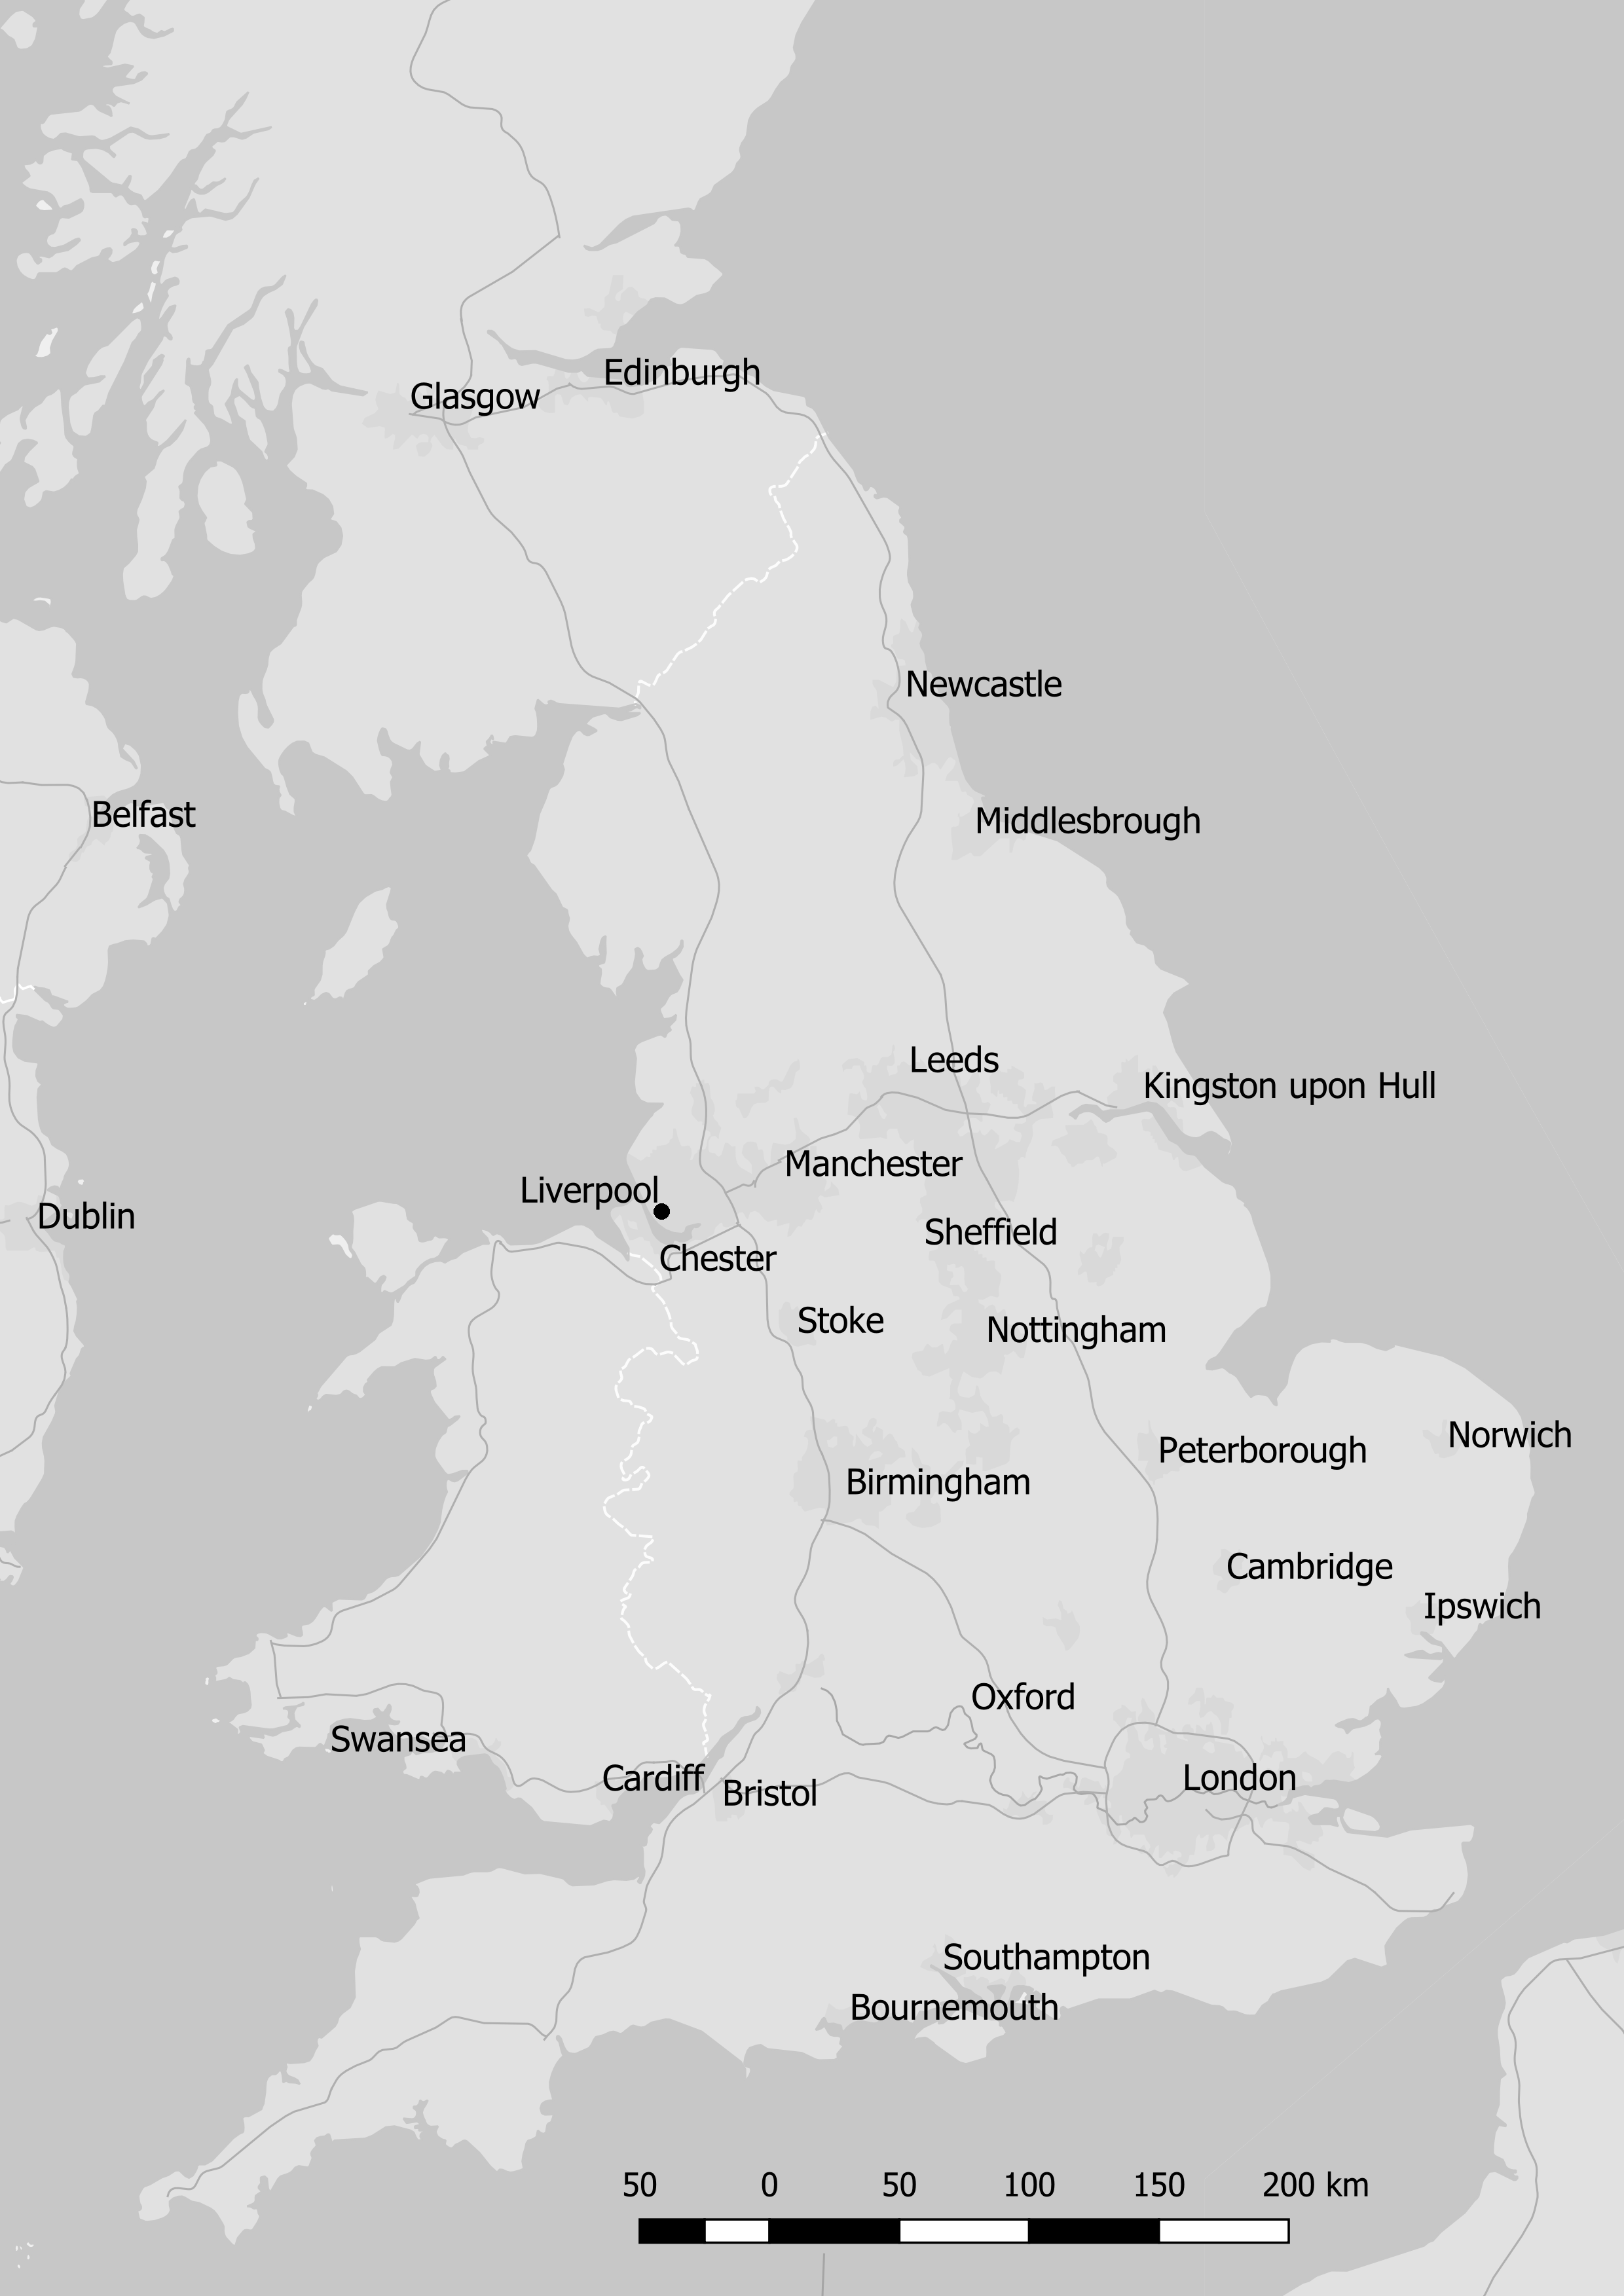
\includegraphics[width=0.5\textwidth]{figures/Map-England.png}
		\caption{Liverpool in the UK}
		\label{fig.ex}
	\end{figure}

	\section{The first 600 years}\label{sec.hist.early}

At the end of the 12\textsuperscript{th} century, \isi{Liverpool}, in the north-west of England (cf. Figure \ref{fig.ex}\footnote{Created with \cite{QGIS2016}. Free vector and raster map data @ naturalearthdata.com.}), was nothing but a very small fishing village in a geographically rather disadvantaged location.
It had neither a parish church nor a castle and its hinterland was ``marginal to the economic and political life of pre-industrial England'' \citep[59]{kermodeetal2006}.
Things began to change when King John granted \isi{Liverpool} borough status in 1207, an act now widely considered as the birth of the city. 
\isi{Liverpool} was a planned town born out of the king's need for a port of embarkation for his campaigns in Ireland.
The city's most long-lasting cultural connection thus originally started out as a military one \citeyearpar[cf.][59--63]{kermodeetal2006}.

In the early 17\textsuperscript{th} century, \isi{Liverpool} had still not grown beyond its original seven streets, indicating that there was no significant population pressure.
The total population of \isi{Liverpool} in 1600 is estimated at around 1000 people, making it about the same size as Lancaster or Blackburn, and only between a fifth and a sixth the size of \isi{Manchester} and Chester.
Commercial activity was modest and remained geographically limited, although \isi{Liverpool} was already used as a port for exporting Lancashire coal, timber, and textiles in these days, and occasional trade with south-western France and northern Spain took place \citeyearpar[cf.][72--76 and 81--84]{kermodeetal2006}.
The latter part of the 17\textsuperscript{th} century saw the establishment and rapid development of new routes, most notably to the West Indies and \isi{Liverpool} ended up overtaking Chester, which had been the major port of the region until then \citep[cf.][107--110]{kermodeetal2006}.

The general increase in international trade in the second half of the 17\textsuperscript{th} and the first half of the 18\textsuperscript{th} century stimulated growth in all European ports, and in Britain the cities facing west, for obvious reasons, prospered in particular.
\isi{Liverpool} became the ``focal point'' of a series of road and canal developments in the area, facilitating transport of Lancashire coal and Cheshire salt to the port \citep[129]{longmore2006}.
The sugar and tobacco trade brought ever greater wealth and a constant flow of work migrants from Lancashire, Cheshire, North Wales and Ireland to the bustling port on the Mersey.
Between 1700 and 1750 the population trebled to around 18,000, with the majority of the immigrants coming from \isi{Liverpool}'s immediate hinterland \citep[cf.][114--119 and 169]{longmore2006}.

Right from the beginning of the 18\textsuperscript{th} century, \isi{Liverpool} also participated in one of the most horrible activities of the period: the slave trade.
In fact, \isi{Liverpool} became ``Britain's leading slave port'' with about 5000 voyages in a bit more than 100 years.
While exact figures are difficult to come by, it is estimated that in excess of 40\% of \isi{Liverpool}'s wealth were due to the slave trade.
Expansion was not halted when the slave trade was finally abolished.
Merchants had already diversified their activities, resulting in a thirty-fold increase of \isi{Liverpool}'s tonnage in the 18\textsuperscript{th} century \citep[cf.][131--134 and 137]{longmore2006}.

It can be argued that at the time this enormous commercial success (admittedly only of a wealthy few) ``provided an alternative identity for the port'' since \isi{Liverpool} did not have much of a medieval heritage to draw on (unlike a lot of other provincial towns of the period, e.g. Bristol, Leeds, or Hull).
Despite a rather transitory pattern of residence (even many merchant families only stayed in the city for three generations or less) \isi{Liverpool} thus managed to create a perceived ``cultural (\ldots) distinctiveness which has arguably remained to the present day''. Due to its international business contacts, the city had a ``cosmopolitan outlook'' and seemed to lie ``outside the culture of Lancashire'' \citep[152--154]{longmore2006}.

For \citet[28]{crowley2012} this is actually the point when \isi{Scouse} as a distinctive variety emerged.
Disagreeing with the `received' version of \isi{Scouse} history that places the beginnings of \isi{Scouse} in the 19\textsuperscript{th} century (cf. \ref{sec.hist.19}), he claims that ``given the population statistics, (\dots) it would make more sense to argue that if a new linguistic form was created in \isi{Liverpool}, then its development surely began (and the form may have even been established) in the eighteenth century''.
His argument is that (in relative terms) the biggest increase in \isi{Liverpool}'s population occurred during this period.
He does acknowledge that most of the people moving into \isi{Liverpool} in the 18\textsuperscript{th} century came from Lancashire but insists that ``the various ports of Cheshire, North Wales and \isi{Wirral} also contributed, to say nothing of those who migrated from Ireland, Scotland, America and the West Indies''.
\citeauthor{crowley2012} seems to forget for the moment that Lancashire and Cheshire form a \isi{dialect} continuum and that the ports of Cheshire and the \isi{Wirral} (historically part of Cheshire anyway) would therefore not have contributed anything radically different in linguistic terms.
The immediate ``rural hinterland'', however, provided most of the incoming population, particularly at the beginning of the 18\textsuperscript{th} century \parencite[cf.][119]{longmore2006}.

Although the city did indeed continue to grow exponentially (around 77,000 inhabitants by 1800) and notwithstanding its `cosmopolitan outlook', the population of \isi{Liverpool} remained rather `un-exotic'.
For instance, very few slaves were brought back to \isi{Liverpool} and those that were sadly died ``almost entirely'' as ``young men, young women and children''.
\citeauthor{longmore2006} further notes that, these few exceptions aside, there seems to be little evidence of a black presence at the time and the current black community therefore must have been established later \citeyearpar[cf.][161 and 169]{longmore2006}. \citeauthor{belchemmacraild2006}, on the other hand, maintain that by the late 1700s a ``vibrant black community'' had developed. However, this community seems to have been very small (contemporary comments mention 50 black and mixed-race children in 1787) \citeyearpar[324]{belchemmacraild2006}.

\citeauthor{crowley2012} also provides some textual evidence for his claim. One of his sources is an early 19\textsuperscript{th} century historian who --- in \citeauthor{crowley2012}'s words --- asserts that ``the Irish presence in \isi{Liverpool} not only grew [in the 18\textsuperscript{th} century], it also contributed to the formation of a distinctive local culture'' \citeyearpar[30]{crowley2012}.
However, the source does not mention accent or \isi{dialect} in any way, but rather talks about ``local manners in the town'' like ``hospitality, activity and sprightliness'' (\citealt{troughton1810}, cited in \citealt[30]{crowley2012}).
Another one is a play first published and performed in \isi{Liverpool} in 1768.
In this play a doctor from \isi{Liverpool} is urged not to forget the `Lancashire \isi{dialect}' when impersonating a cousin from outside the city.
\citeauthor{crowley2012}'s point is that this should be seen as evidence for the fact that ``the speech of at least some of the inhabitants of \isi{Liverpool} was not the same as that of Lancastrians'' \cite[cf.][32--35]{crowley2012}.

This is hardly hot news.
After all, given the language-related ideology already in place at the time (as \citeauthor{crowley2012} himself points out on page 23) no-one would expect a doctor, a well-respected and educated member of the middle-class, to use a pronounced regional accent.
The passages that \citeauthor{crowley2012} quotes merely indicate that middle-class Liverpudlians were not speaking with a broad Lancashire accent, not that they had developed their own.
To be fair, \citeauthor{crowley2012} himself remarks on the fact that his textual evidence --- just like that of the proponents of the `received version' --- is rather thin.
It appears even less convincing if one considers that, according to oral historians, ``many working-class Liverpudlians failed to exhibit any `\isi{scouse}' (sic) characteristics (\ldots) in their speech until well into the twentieth century''  \citep[43--44]{belchem2006d} --- more than 100 years after the variety had been coined if \citeauthor{crowley2012} is correct.


	\section{19\textsuperscript{th} century}\label{sec.hist.19}

From a linguist's point of view, things in \isi{Liverpool} really start to get interesting in the 19\textsuperscript{th} century, but not much before --- although we have seen above that there is at least one scholar who disagrees with this `received' version of the history of \isi{Scouse}.
It is, however, generally agreed that \isi{Liverpool} English is ``a relatively new variety of English'' where ``[a]ll the evidence'' suggests emergence ``from a \isi{dialect} mixture'' \citep[113 and 121]{honeybone2007}.
\citeauthor{honeybone2007} distinguishes three stages in the development of the ``\isi{perceptually} distinct \isi{Liverpool} English that now exists (\dots)'' \citeyearpar[119]{honeybone2007}:

	\begin{description}
		\item[Stage 1] broadly pre-19th century
		\item[Stage 2] (especially mid) 19th century
		\item[Stage 3] broadly post-19th century
	\end{description}

He further states that stage 2 is the period ``when the available evidence indicates that the variety came into being'', at a time ``when speakers of a number of dialects were mixing in the area'' \citeyearpar[106--107]{honeybone2007}.
And speakers of a number of dialects certainly did mix in \isi{Liverpool} in the 19\textsuperscript{th} century.
From 1801 to 1901, the population increased almost nine-fold --- from around 82,000 to 711,000 \parencite{gbhistgis}.
This, in itself, is nothing out of the ordinary.
Most major cities, in Britain as in other industrialised countries, \enquote*{exploded} during the Victorian era.
\isi{Manchester}, for instance, also went from 88,000 in 1801 to 642,000 in 1901 \parencite{gbhistgis}.
An additional factor is important to understand \isi{Liverpool}'s particular development at the time.

In urban geography, cities are often classified according to two theories, the central place model and the network model.
A central place acts as an administrative and economic centre that provides `services' for its hinterland. Classical examples are medieval market towns.
A network city, on the other hand, is a node in an often international system of cities and as such is less dependent on and in less intense contact with its hinterland compared to a central place.
Important ports are \isi{prime} examples of this type of city.
Obviously, the two functions often overlap and many towns or cities are both central places and network cities.
In the Northwest, ``\isi{Liverpool} and \isi{Manchester} divided the functions of a regional capital'', with \isi{Manchester} being the ``summit of the array of central places'' and \isi{Liverpool} fulfilling the function of ``gateway city linking the region to European and trans-Atlantic urban networks'' \citep[188--189]{hohenberglees1985}.

When the slave trade was finally abolished in 1807, \isi{Liverpool} turned to raw materials like timber, oils, and especially cotton.
These raw materials, along with ``the plethora of goods demanded by an urbanizing population'' were needed by \isi{Liverpool}'s hinterland, ``the manufacturing powerhouse that was north-west England''.
The goods produced in \isi{Manchester} and the rest of Lancashire and Cheshire were then exported through \isi{Liverpool}'s port to the four corners of the globe.
Diversity of goods increased and \isi{Liverpool} turned into one of the 19\textsuperscript{th} century's only two ``general cargo giants'' in Britain (the other one being London).
New trading contacts were established in India, China, and South America \citep[cf.][258--259]{milne2006}.
\isi{Liverpool} increasingly felt at the heart of a global maritime network.
At least to a degree this was certainly justified.
After all, it had become the second biggest city and the most important port in the country by 1850 \citep[cf.][113--114]{honeybone2007}.

In addition to its importance as one of the busiest cargo ports in the world, \isi{Liverpool} also acquired another function.
Around 1850, the city had established itself as the principal emigration port of the old world (especially for those bound for the United States) and acquired the nick name `New York of Europe' \parencite[xxvii]{belchem2006c}.
By way of example, \citet[14]{belchem2006a} notes that in 1851 alone, 455 ships sailed from \isi{Liverpool} to New York, compared to 124 for Le Havre and 132 for Bremen.
He goes on to explain that more than 85\% of the 5.5 million Europeans that emigrated to America between 1860 and 1900 did so from or through \isi{Liverpool}.
These emigrants, although their presence was usually only transitory, turned \isi{Liverpool} into a `diaspora space' and further enhanced its ``cosmopolitan complexion''.

If contemporary commentators are to be believed, immigrants, travellers, and sailors from all around the world were generally given a friendly welcome by the locals.
An anonymous source counts ``[h]ospitality, social intercourse, civility to strangers, and that freedom from local prejudice which is produced by the residence of so great a proportion of strangers'' among the ``very favourable features in the general portrait'' of \isi{Liverpool} people (\citealt{anon1812}, cited in \citealt[12]{crowley2012}).
Apparently, this hospitality was also extended to visitors of other races.
\citet[13]{belchem2006a} notes that ``[b]lack passengers in transit were delighted by their reception when they ventured into town, even into the established church''.
\citeauthor{belchem2006d} also cites a contemporary comment from 1907, describing the Pier Head and the central landing-stage as the place where all of \isi{Liverpool} met either for business or pleasure reasons and that ``encouraged social intermingling'' and had the ``appearance of a democratic promenade'' (\citealt{scott1907}, cited in \citealt[45]{belchem2006d}).

Due to these intensive international contacts, \citet[15]{knowles1973} claims that ``[t]he important linguistic ties'' are less with the Lancashire hinterland, and more with ``Dublin and London and the whole of the English speaking world''.
He assumes that \isi{Scouse} emerged as a distinct variety some time between 1830 and 1889, which ``corresponds with the period of massive immigration from Ireland'' \citeyearpar[18]{knowles1973} during and after the Irish Potato Famine (1845--1852).
This is crucial for \citeauthor{knowles1973}, who describes \isi{Scouse} as being a still essentially north-western variety that has been heavily influenced by Irish immigrants \citeyearpar[cf.][51]{knowles1973}.
Applying Trudgill's model of new \isi{dialect} formation \citep{trudgill1986,trudgill2004} to \isi{Liverpool}, \citeauthor{honeybone2007} provides similar dates (1841 to 1891) for the emergence of \isi{Scouse} but is less categorical with respect to the Irish role in the matter.
He explains that, somewhat surprisingly, there was no pronounced founder effect privileging North-Western English although clearly no \emph{tabula rasa} situation existed in \isi{Liverpool} in the 19\textsuperscript{th} century.
At the same time, Irish English was not simply transplanted wholesale to \isi{Liverpool} \citep[cf.][117 and 121]{honeybone2007}.

This is not to say that Irish immigrants were \emph{not} a crucial factor in the formation of \isi{Liverpool} culture and language.
Their sheer number argues against such ideas.
Even before the famine, many Irish emigrated to \isi{Liverpool}, because it was ``the obvious, indeed often unavoidable place to go from Ireland as it was the main port of Britain on the West coast, facing Ireland''.
Many also originally meant to travel to the United States or other places but ended up staying in \isi{Liverpool} for good  \citep[cf.][114 and 117]{honeybone2007}.
As can be gleaned from Table \ref{tab.birthplace} (adapted from \cite[249]{pooley2006}), about one in five Liverpudlians in the middle of the century had been born in Ireland.
This is a sizeable proportion and it has to be borne in mind that people with Irish ancestry but who had been born in \isi{Liverpool} are not even included in this count.

	\begin{table}[h]
		\centering
		\caption{Selected birthplaces of Liverpudlians in the 19\textsuperscript{th} century}
		\begin{tabular}{lrrr}
			\hline
			Birthplace & 1851 & 1871 & 1891 \\ 
			\hline
			Lancashire & \multirow{2}{*}{50.3\%} & \multirow{2}{*}{58.7\%} & \multirow{2}{*}{68.9\%} \\
			(including \isi{Liverpool}) & & & \\
			Ireland & 22.3\% & 15.6\% & 9.1\% \\ 
			Wales & 5.4\% & 4.3\% & 3.4\% \\ 
			Scotland & 3.7\% & 4.1\% & 3.0\% \\
			Cheshire & 3.4\% & 3.0\% & 2.8\% \\ 
			\hline
		\end{tabular}
		\label{tab.birthplace}
	\end{table}

A number of problems arise if one is to take \citeauthor{knowles1973}' view and consider Irish English speakers as the dominating influence in the creation of \isi{Scouse}.
The Irish were
\begin{inparaenum}[a\upshape)]
	\item highly concentrated --- one might say ghettoised --- in certain parts of the city, 
	\item ``only ever an absolute majority in few streets'' \citep[120]{honeybone2007}, 
	\item generally of a lower socio-economic status than people born in \isi{Liverpool}, and
	\item for the most part Roman Catholics \citep[cf.][330]{belchemmacraild2006}.
\end{inparaenum}
These features add up to a spatially isolated and heavily stigmatised group of \isi{Liverpool} society at the time.
Under these circumstances, it is very difficult to argue convincingly that ``their speech would swamp the dialects of inmigrants from other areas'', as \citet[120]{honeybone2007} rightly points out.
What is more, the proportion of Irish migrants was similar in other cities.
\citet[140]{honeybone2007} cites 18.1\% and 13.1\% for Glasgow and \isi{Manchester} in 1851 respectively, so the number of speakers alone cannot account for the particular linguistic development in \isi{Liverpool}.

Table \ref{tab.birthplace} also indicates that there was a non-negligible community of Welsh and Scots (more than 9\% in 1851, again not counting second and third generation immigrants).
These figures are small compared to the Irish part, but they were still large enough for \isi{Liverpool} to acquire the nickname `capital of North Wales' and to boast the second-largest Scots community in England.
Neither Welsh nor Scots were spatially as concentrated as the Irish although they did constitute what \citeauthor{honeybone2007} calls ``highly organised'', i.e. somewhat inward-looking and self-sufficient communities \citep[cf.][120--121]{honeybone2007}.
Unlike the Irish, these groups were associated with the skilled working population \citep[cf.][202--203]{belchem2006b}, which makes their dialects more likely contributors to the emerging \isi{Scouse} than the varieties spoken by a non-prestigious group like the Irish.
To these larger minorities, one must add smaller numbers of people not represented in Table \ref{tab.birthplace} --- from all over Britain, Africa, the Caribbean, and China.
All of these people have, in some way, contributed to the \isi{dialect} mix in the city \citep[cf.][116]{honeybone2007}.

Knowles and Honeybone disagree to an extent about which influences most shaped early \isi{Scouse}.
However, both assert, the former on the basis of somewhat cryptic comments in \citealt{ellis1889} \citep[cf.][18]{knowles1973}, the latter using Trudgill's new-\isi{dialect} model \citep[cf.][118]{honeybone2007}, that by the end of the 19\textsuperscript{th} century a variety identifiable as `\isi{Liverpool} English' had been created.

	\section{20\textsuperscript{th} century}\label{sec.hist.20}

		\subsection{Enregisterment and the `Scouse industry'}\label{sec.hist.20.industry}

\isi{Liverpool} continued to grow in the 20\textsuperscript{th} century, reaching its population pinnacle of around 855,000 in 1931 \citep[cf.][171]{pooley2006}, despite the fact that \isi{Liverpool}'s economic vulnerability showed dramatically during the inter-war years when the world economy slumped and 30\% of port related jobs disappeared over night.
The port acquired outstanding, though short-lived, importance again during World War 2 when \isi{Liverpool} was the European end point of the Allied convoys and the command centre for the Battle of the Atlantic (a fact which also made it a \isi{prime} target for the Luftwaffe which wreaked considerable destruction on the city and killed thousands of people in 1940--1941) \citep[cf.][393 and 405]{murden2006}.
While immigration from all parts of the word continued \citep[cf.][119]{honeybone2007}, attitudes towards migrants got less positive, at least in some parts of \isi{Liverpool} society.
At times ``hysterical reaction[s]'' in the local press can now be seen as precursors of the ``troubled pattern of `racialized relations''' in the latter part of the 20\textsuperscript{th} century \citep[cf.][23]{belchem2006a}.

At around the same time (the early to mid-20\textsuperscript{th} century) developed what \citet[40]{crowley2012} calls the ``\isi{Scouse} industry''.
From the 30s onwards, a number of articles and letters to the editors in local newspapers discussing `\isi{Liverpool}' words and phrases can be found.
While most of these claims were incorrect --- \citet[48]{knowles1973} comments on ``the very paucity of the material'' particular to \isi{Scouse} in the domain of grammar and vocabulary --- they nevertheless ``indicated that there was a developed sense that \isi{Liverpool} as a place had a vocabulary (and a mode of pronunciation) that was part of its cultural distinctiveness within Britain'' \citeyearpar[42]{crowley2012}.
In other words, \emph{enregisterment} was well under way, and \isi{Scouse} was turning --- or had already turned --- into a ``socially recognised register of forms'' that was ``differentiable within [the] language'' \parencite[231]{agha2003}.
In the years following World War 2, two individuals in particular gained publicity in this domain and are still well-known today.
Neither Frank Shaw nor Fritz Spiegl were linguists (Shaw worked as a customs officer, Spiegl was a flutist), but rather amateurs (in the original sense) who ran a campaign to ``present \isi{Scouse} as the language of \isi{Liverpool}'' and who tried to ``popularize, celebrate and preserve aspects of the language and culture of \isi{Liverpool}'' \citep[64--65]{crowley2012}.
The \emph{Lern Yerself Scouse} series sparked off by these two in the 60s can still be found in most \isi{Liverpool} book shops today.
On the surface at least, these short booklets were intended as a sort of phrasebook for visitors of the city, familiarising them with vocabulary and pronunciations peculiar (in the authors' opinion) to \isi{Liverpool} English (\citet{honeybonewatson2013} provide a linguistic analysis of these volumes; cf. also Chapter \ref{ch.var}).

Although the series may well be considered ``the touchstone for the \isi{Scouse} industry'' \citep[79]{crowley2012}, it was clearly not its only manifestation.
As early as the 1930s, the city had established for itself a ``reputation for humour'' that was carried on in the 60s by people like Ken Dodd and Jimmy Tarbuck, both in theatres across the country and on TV (cf. \citealt[423]{murden2006}, and \citealp[49]{belchem2006a}).
\isi{Liverpool} was also represented on national TV in the 50s and 60s with series like \emph{Z-Cars} or \emph{The Liver Birds}, which showed characters that ``often conformed to the cultural, linguistic and social representations that had been set out by the founders of the \isi{Scouse} industry''.
Finally, numerous pop bands came out of \isi{Liverpool} during the Merseybeat era, the most famous and influential of which were the \isi{Beatles}, who acquired unprecedented fame for \isi{Liverpool} and, at least for a couple of years, made the city the centre of the pop music world \citep[cf.][75]{crowley2012}, while ``Britain fell in love with everything connected to \isi{Liverpool}'' \citep[423]{murden2006}.

Based on his textual/literary evidence, \citet[107]{crowley2012} claims that the stage of ``first-order (sic) \isi{indexicality} with regard to \isi{Liverpool} speech'' was reached ``in the early to mid twentieth century''.
His argument is that ``there is clear evidence that words and sounds were postulated (often incorrectly) as belonging uniquely to \isi{Liverpool}''.
Since these postulations stem from non-experts, however, we are at this point dealing with \isi{third-order indexicality} already, since the peculiarities have started attracting explicit comment.
This must be a typographical error, otherwise \citeauthor{crowley2012}'s claim is even more strange if we \isi{remember} him arguing elsewhere that \isi{Scouse} emerged from dialect-mixing in the 18\textsuperscript{th} century already (cf. \ref{sec.hist.early}).
Based on \citeauthor{silverstein2003}' \citeyear{silverstein2003} orders of \isi{indexicality}, \textcite[81]{johnstoneetal2006} define first-order \isi{indexicality} as ``the kind of correlation between a form and a sociodemographic identity (\ldots) that an outsider could observe'', i.e. experts can identify a feature as being indicative of a particular group of speakers, possibly even while the variety is still emerging.
Crucially, however, this features does not yet do social work (second-order \isi{indexicality}), nor is it talked about or used in \isi{conscious} performances (\isi{third-order indexicality}) of \isi{local identity} \parencite[cf.][83--84]{johnstoneetal2006}.

Nevertheless, \citeauthor{crowley2012} correctly explains that the comments by Shaw and others, distinguishing `real Liverpudlians' from `middle-class Mossley Hill Liverpolitans' to use Shaw's phrasing, indicate (at least) second-order \isi{indexicality}, since \isi{social stratification} was, apparently, firmly in place with respect to \isi{Liverpool} English, which is why it had already become ``the index not simply of \isi{Liverpool} identity, but of \isi{Liverpool} working-class identity'' \citep[107]{crowley2012}.
When some features of \isi{Scouse} definitely reached \isi{third-order indexicality} in the 60s, this association with the working-class was less of a problem than several decades before and might even have contributed to the `coolness' (The `\isi{Liverpool} cult' --- \citealt[109]{crowley2012}) of the \isi{Scouse} identity.
As \citet[165]{wales2006} notes, ``it became fashionable to be young, working class and urban, and the importance of this on \isi{language change} in the late twentieth century should not be underestimated''.

		\subsection{Decline}\label{sec.hist.20.decline}

While \isi{Liverpool} was enjoying its heyday in terms of image and popularity it was already facing serious difficulties in other respects. After a short revival in the 1950s \citep[cf.][402]{murden2006}, economic decline hit the city hard from the 1960s and especially the 1970s onwards.
Following the 1973 oil crisis most western countries went into recession and thousands of manufacturing jobs were lost.
While new service jobs countered this loss, they usually developed in other regions (in the case of Britain the south of England) than those most affected by structural change (northern England) \citep[cf.][16--17]{juddparkinson1990a}.

\isi{Liverpool} had prospered enormously as a trading hub in the Victorian era, but the end of the empire, the ``collapse of the colonial economic system'' \citep[52]{belchem2006a}, and Britain's (economic) shift of focus towards Europe meant that \isi{Liverpool} ``found itself poorly located to take advantage of the increasing trade between the UK and mainland Europe'' that now dominated \citep[166--167]{couch2003a}.
In addition to that, containerisation meant that even the few ports that were able to retain their importance (Rotterdam and Hamburg alone ended up serving all of northern Europe, cf. \citealt[264]{milne2006}) did not require thousands of workers any more but just a handful of more specialised employees to operate the machinery.
Due to its container terminal in Seaforth \isi{Liverpool}'s port today handles more cargo than ever before, but it does so with a workforce of only 800 (7000 in the whole maritime sector, figures for 2003, \citealt[cf.][477]{murden2006}).

The central government tried to fight unemployment by encouraging private investors to open up new factories in the city, but in most cases success was short-lived.
The militancy of \isi{Liverpool} workers --- ``a myth in the making'' --- was often used as a pretext whenever \isi{Merseyside} plants were the first to be closed again ``[o]nce development aid and other short-term advantages were exhausted''\citep[cf.][52]{belchem2006a}.
\isi{Liverpool} became the ``beaten city'' and a ```showcase' of everything that has gone wrong in Britain's major cities'' \citep[\emph{Daily Mirror}, 11 October 1982, cited in][52--53]{belchem2006a}.

While claims concerning the militancy of Liverpudlians in general might well have been more based on stereotypes than fact, there certainly was \emph{political} militancy in the form of Militant Tendency (a Labour `sect') in the 1980s.
Until 1979, central government measures were focused on social and welfare services on the one hand and the creation of public sector jobs on the other. When Margaret Thatcher became \isi{prime} minister, however, urban policy changed \citep[cf.][19]{juddparkinson1990a}.
Public spending was to be cut back considerably.
The Militant majority of \isi{Liverpool} City Council disagreed and, in the eyes of some at least, tried to \enquote{force} the government into granting them additional funds and effectively ``threaten[ed] to bankrupt the city if it were not given the extra resources''.
In 1987 the House of Lords finally disqualified 47 Labour officials of the City Council from office for failing to protect the financial interest of the city \citep[cf.][249--250]{parkinson1990}.
The damage had been done, however.
\isi{Liverpool}'s ``political failure'' \citep[241]{parkinson1990} resulted in a ``sharp decline in investor confidence'' and a ``deterioration in the image of the city'' which lasted for many years \citep[172]{couch2003a}.

Economic decline was followed by physical deterioration.
In the 80s, Central \isi{Liverpool} was fast losing population and jobs, the shopping centre had to yield business to retail parks in the suburbs, congestion was on the rise and environmental conditions went downhill \citep[cf.][38]{couch2003}.
This ``visual legacy of dereliction'' brought with it an ``air of decay'' which made the area even less attractive to potential private sector investors and thereby created or at least contributed to a downward spiral of recession and decay \citep[21]{fraser2003}.

Due to these economic problems (and the limited opportunities for migrants that ensued), \isi{Liverpool} did not participate in the post-war mass-immigration from the Caribbean and South Asia in the same way as other major British cities did.
While \isi{Liverpool} was, after London, the most ethnically diverse British city in the 19\textsuperscript{th} century, it is clear from Table \ref{tab.ethnicity} (data are from \citealt{nomis}) that this is no longer true.
In fact, although minorities now make up a larger proportion of \isi{Liverpool} residents than in 2001 (largely due to a recent influx of refugees and asylum seekers), it is today still one of the \emph{least} ethnically diverse places in Britain, clearly outdone by \isi{Manchester} in this respect and a far-cry from places such as Birmingham or London \citep[cf.][187]{pooley2006}.

	\begin{table}[h]
		\centering
		\caption{Ethnicity in Liverpool and other major cities (\%)}
		\begin{tabular}{lrrrrrrrr}
			\hline
	 		& \multicolumn{2}{c}{Liverpool} & \multicolumn{2}{c}{Manchester} & \multicolumn{2}{c}{Birmingham} & \multicolumn{2}{c}{London} \\
			 & 2001 & 2011 & 2001 & 2011 & 2001 & 2011 & 2001 & 2011 \\
			 \hline
			 white & 94.32 & 88.91 & 80.96 & 66.61 & 70.35 & 57.93 & 71.15 & 59.79 \\
			 black & 1.22 & 2.64 & 4.51 & 8.64 & 6.12 & 8.98 & 10.92 & 13.32 \\
	 		 Asian & 2.27 & 4.16 & 10.44 & 17.09 & 20.04 & 26.62 & 13.20 & 18.49 \\
	 		 mixed & 1.80 & 2.52 & 3.23 & 4.60 & 2.86 & 4.44 & 3.15 & 4.96 \\
	 		 other & 0.39 & 1.77 & 0.86 & 3.06 & 0.63 & 2.03 & 1.58 & 3.44 \\
	 		 \hline
		\end{tabular}
		\label{tab.ethnicity}
	\end{table}

In addition to that, \isi{Liverpool}'s minority population is (and always has been) highly concentrated (segregated?) in central areas of the city.
Furthermore, the ``most visible'' minorities --- especially blacks and Chinese --- had to endure marginalisation and a certain degree of racial violence from the early 20\textsuperscript{th} century onwards \citep[cf.][189--191]{pooley2006}.
Racial tensions and more general disappointment with the authorities culminated in the Toxteth riots of 1981 which lasted for two weeks, caused \pounds11 million of damage, and left hundreds of people (police and civilians) injured and one dead \citep[cf][440--444]{murden2006}.

All of this had an impact on evaluations of the primary expression of \isi{Liverpool} culture, \isi{Scouse}.
\isi{Scouse} received poor popular ratings already in the 1970s and this was corroborated in a 1990s survey where \isi{Scouse} got an approval rating of only 6\%, while at the same time frequently joining other Northern accents in scoring rather high for `friendliness' \citep[cf.][166]{wales2006}.
What is even more important than the negative \emph{external} perceptions of \isi{Liverpool} and \isi{Scouse} is what \citet[255]{parkinson1990} calls an ``\isi{internal image} problem''.
Writing in \citeyear{parkinson1990}, he claims: 
	\begin{quote}
		Two decades of economic failure, compounded by political failure and self-destruction, have bred a degree of cynicism in the city's public life. There is clearly a cultural dimension to the city's failure that goes beyond the statistics of economic decline.
	\end{quote}
It probably goes without saying that this ``cultural dimension'' is highly likely to include the linguistic domain as well.
It would not be surprising if an ``\isi{internal image} problem'' impacted on people's (socio-)linguistic behaviour, i.e. if at least some speakers tried to tone down their local accent a bit because they felt it to be somewhat contaminated by the negative associations attached to the city.
If this was the case then it may well have helped bring about, or at least accelerate, what \citet{knowles1978} calls the `extensive standardisation' of \isi{Scouse} in the 20\textsuperscript{th} century.

		\subsection{Regeneration}\label{sec.hist.20.regen}

Politicians in \isi{Liverpool} and London did not just passively watch the city's physical decline.
Post-war measures mostly focused on public housing, inner city slum clearance and relocation of the population to new housing estates on the periphery.
From the beginning of the 1980s, the strategy slowly started to change.
The emphasis was now on the ``potential of the city center in terms of retail, leisure, tourism, and commercial development''.
The city council even funded studies evaluating the tourist potential and dealing with things like \isi{Liverpool}'s bad image and city marketing \citep[cf.][250--253]{parkinson1990}.

Decline continued all the same and in 1993 \isi{Liverpool} (and the whole region of \isi{Merseyside} to be exact) had spiralled down into Objective One status --- a label given by the EU to regions whose GDP per capita is 75\% or less of the EU average.
\citet[53--54]{belchem2006a} notes that ``[a]lthough at the time it seemed a badge of failure'' this may well turn out to have been a ``decisive turning point for the city'', because it gave access to considerable European funds.
In its wake, the city council turned towards ``urban entrepreneurialism, partnership governance and civic boosterism'', which is very unlike the political style that was prevalent in the 80s.

Economically, it had become clear, in \isi{Liverpool} and elsewhere, that it was not possible to recreate the past.
Instead, the future was seen in information technology and new (tertiary) industries (such as banking and advertising) \citep[cf.][32]{fraser2003}.
A local film industry was also successfully established in the second half of the 80s and the year 1989 saw the creation of the \isi{Liverpool} Film Office, the first of its kind in the UK \citep[cf.][479]{murden2006}.
First and foremost, however, \isi{Liverpool} turned towards tourism and (re-)discovered its cultural heritage as an economic asset \citep[cf.][32--33]{fraser2003}.
The city centre was physically improved through things like new squares, public spaces, and pedestrianised shopping areas.
The waterfront with its unused docks and warehouses has proved particularly suitable for regeneration as a tourist and leisure area \citep[173--174]{couch2003a}.

Regeneration did (and does) also face problems.
Just like in other places in the UK, the ``private development sector'' is rather powerful.
As a consequence, most measures have focused on high-return investments in the city centre with an ensuing neglect of more peripheral areas like Vauxhall or North \isi{Liverpool} that are just as much (or even more) in need of regeneration \citep[cf.][49]{couch2003}.
Furthermore, \isi{Liverpool} is in competition with \isi{Manchester}, which is now the undisputed regional capital thanks to its airport (the most important one outside London) and its more central location.
As such, \isi{Manchester} was (and still is) often the more obvious choice for potential investors in the north-west.
While the ``deep-seated social and economic problems (\ldots) still remain acute'' \citep[188]{fraser2003a}, it is all the same important to \isi{remember} that ``a great deal [was achieved], at least in terms of physical change'' \citep[44]{couch2003}.

Due to the fact that private investors were now operating on an international level it became important for cities to emphasise their local attributes through the use of place promotion and marketing strategies.
Cultural revitalisation, organisations like \isi{Liverpool} Vision and \isi{prestige} projects like the Albert Dock are examples of this attempt to create and foster a new image.
In addition to attracting investment, these projects can also instil pride into local people and thus ``help to promote civic identity'' \citep[cf.][201--203]{percy2003}.

Pride in the city is an important aspect.
\citet[20]{fraser2003} explains that cities past their heyday such as \isi{Liverpool} ``should be vanishing as new centres took their place''.
Obviously, this is not what has happened.
Rather, people try ``to find a new rationale for its existence and re-creation of its former prosperity. \emph{It is a matter of \isi{conscious} choice to do so}'' (my emphasis).
This \isi{conscious} choice not to give up is, among other things, based on ``a \emph{sense of place}, a special character or feeling in and for that place, which attracts loyalty from inhabitants'' \citep[23, emphasis in the original]{fraser2003}.
Successful regeneration might well have filled Liverpudlians with new self-pride and self-respect.
New self-respect in turn should manifest itself in (sub-)\isi{conscious} reinforcement of social markers such as accent.

We might even suspect that the external image of \isi{Scouse} improved as well.
If \citet[73]{trudgill1999} and \citet[110]{honeybone2007} are to be believed, \isi{Scouse} must have had acquired some \isi{covert} \isi{prestige} by the late 1990s and spread not only to Birkenhead, but also to more rural areas in \isi{Merseyside}.
\citet[176--177]{montgomery2007a} even --- speculatively --- suggests that some people from Crewe in Cheshire might identify with \isi{Scouse}.
The fact that a great number of new call centres were established in \isi{Merseyside} in 1998 also casts some doubt on ``the usual stigma attached to \isi{Scouse}'' as ``[t]elesales companies have apparently taken great care to locate their call centres in regions where their workers' accents will be favourably perceived'' \citep[3]{foulkesdocherty1999a}.

	\section{21\textsuperscript{st} century --- outlook}\label{sec.hist.21}

Regeneration continued in the new millennium with a new big convention centre (the Echo Arena) and the transformation of RopeWalks into a modern, hip and trendy leisure quarter housing a media arts centre and numerous bars, restaurants, and clubs.
To the north west, in the very centre of the city, about £920 million were spent on \isi{Liverpool} ONE, one of the largest open-air retail spaces in the UK, but also comprising residential and leisure facilities.
From 2004 to 2008 it completely transformed about 42 acres of previously rather bleak land and, in passing, improved access to the city centre by public transport considerably through the new bus interchange that was part of the project \parencite[cf.][478--479]{murden2006}.
An even bigger development project, \isi{Liverpool} Waters, was granted planning permission in March 2013 and is supposed to create 17,000 jobs while redeveloping the north docks.

\isi{Liverpool} also continued to do well on the culture front.
In 2004, parts of the waterfront and the Cultural Quarter (the area around St. George's Hall and the World Museum) were inscribed on UNESCO's list of World Heritage Sites, a badge which surely further increased \isi{Liverpool}'s attraction as a tourist destination.
The probably most important achievement of the city in the new millennium so far was its success in acquiring the title of European Capital of Culture in 2008 (together with Stavanger in Norway).

Not only did this title provide the occasion and the framework for a year of events and festivals, it also had a number of measurable effects.
As a direct consequence of the title, around 9.7 million additional visitors were counted in 2008, with 97\% of the international tourists visiting for the first time.
More than £750 million of direct income for the city's economy was created this way, and data collected from 2005 to 2010 indicate that the `Capital of Culture' effect could be lasting \parencite{garciaetal2010}.
What may, in the long term, be even more important is that media coverage changed as well.
In the 1990s national media had largely focused on (usually negative) social issues when covering \isi{Liverpool}, while in 2008/2009 ``culture and image stories'' dominated.
Local media showed a pronounced increase in positive coverage in the years leading up to 2008 as well.
Positive impressions about \isi{Liverpool} increased statistically significantly in national surveys from 2005 to 2008 \citep[cf.][25 and 44--46]{garciaetal2010}.

	\begin{figure}[h]
		\centering
		% Created by tikzDevice version 0.10.1 on 2017-03-14 14:20:47
% !TEX encoding = UTF-8 Unicode
\begin{tikzpicture}[x=1pt,y=1pt]
\definecolor{fillColor}{RGB}{255,255,255}
\path[use as bounding box,fill=fillColor,fill opacity=0.00] (0,0) rectangle (202.36,202.36);
\begin{scope}
\path[clip] (  0.00,  0.00) rectangle (202.36,202.36);
\definecolor{drawColor}{RGB}{255,255,255}
\definecolor{fillColor}{RGB}{255,255,255}

\path[draw=drawColor,line width= 0.6pt,line join=round,line cap=round,fill=fillColor] (  0.00,  0.00) rectangle (202.36,202.36);
\end{scope}
\begin{scope}
\path[clip] ( 39.40, 33.48) rectangle (196.36,196.36);
\definecolor{fillColor}{RGB}{255,255,255}

\path[fill=fillColor] ( 39.40, 33.48) rectangle (196.36,196.36);
\definecolor{drawColor}{gray}{0.98}

\path[draw=drawColor,line width= 0.6pt,line join=round] ( 39.40, 48.66) --
	(196.36, 48.66);

\path[draw=drawColor,line width= 0.6pt,line join=round] ( 39.40, 87.87) --
	(196.36, 87.87);

\path[draw=drawColor,line width= 0.6pt,line join=round] ( 39.40,127.08) --
	(196.36,127.08);

\path[draw=drawColor,line width= 0.6pt,line join=round] ( 39.40,166.29) --
	(196.36,166.29);
\definecolor{drawColor}{gray}{0.90}

\path[draw=drawColor,line width= 0.2pt,line join=round] ( 39.40, 68.27) --
	(196.36, 68.27);

\path[draw=drawColor,line width= 0.2pt,line join=round] ( 39.40,107.48) --
	(196.36,107.48);

\path[draw=drawColor,line width= 0.2pt,line join=round] ( 39.40,146.69) --
	(196.36,146.69);

\path[draw=drawColor,line width= 0.2pt,line join=round] ( 39.40,185.90) --
	(196.36,185.90);

\path[draw=drawColor,line width= 0.2pt,line join=round] ( 68.83, 33.48) --
	( 68.83,196.36);

\path[draw=drawColor,line width= 0.2pt,line join=round] (117.88, 33.48) --
	(117.88,196.36);

\path[draw=drawColor,line width= 0.2pt,line join=round] (166.93, 33.48) --
	(166.93,196.36);
\definecolor{fillColor}{gray}{0.20}

\path[fill=fillColor] ( 46.76, 40.88) rectangle ( 57.79,146.69);
\definecolor{fillColor}{RGB}{129,129,129}

\path[fill=fillColor] ( 57.79,108.83) rectangle ( 68.83,146.69);
\definecolor{fillColor}{gray}{0.67}

\path[fill=fillColor] ( 68.83,119.87) rectangle ( 79.87,146.69);
\definecolor{fillColor}{gray}{0.80}

\path[fill=fillColor] ( 79.87,118.63) rectangle ( 90.90,146.69);
\definecolor{fillColor}{gray}{0.20}

\path[fill=fillColor] ( 95.81,130.96) rectangle (106.84,146.69);
\definecolor{fillColor}{RGB}{129,129,129}

\path[fill=fillColor] (106.84,146.69) rectangle (117.88,148.24);
\definecolor{fillColor}{gray}{0.67}

\path[fill=fillColor] (117.88,146.56) rectangle (128.91,146.69);
\definecolor{fillColor}{gray}{0.80}

\path[fill=fillColor] (128.91,130.53) rectangle (139.95,146.69);
\definecolor{fillColor}{gray}{0.20}

\path[fill=fillColor] (144.85,146.69) rectangle (155.89,188.95);
\definecolor{fillColor}{RGB}{129,129,129}

\path[fill=fillColor] (155.89,139.53) rectangle (166.93,146.69);
\definecolor{fillColor}{gray}{0.67}

\path[fill=fillColor] (166.93,132.29) rectangle (177.96,146.69);
\definecolor{fillColor}{gray}{0.80}

\path[fill=fillColor] (177.96,146.69) rectangle (189.00,158.45);
\definecolor{drawColor}{gray}{0.50}

\path[draw=drawColor,line width= 0.6pt,line join=round,line cap=round] ( 39.40, 33.48) rectangle (196.36,196.36);
\end{scope}
\begin{scope}
\path[clip] (  0.00,  0.00) rectangle (202.36,202.36);
\definecolor{drawColor}{RGB}{0,0,0}

\node[text=drawColor,anchor=base east,inner sep=0pt, outer sep=0pt, scale=  0.80] at ( 34.00, 64.96) {-50};

\node[text=drawColor,anchor=base east,inner sep=0pt, outer sep=0pt, scale=  0.80] at ( 34.00,104.17) {-25};

\node[text=drawColor,anchor=base east,inner sep=0pt, outer sep=0pt, scale=  0.80] at ( 34.00,143.38) {0};

\node[text=drawColor,anchor=base east,inner sep=0pt, outer sep=0pt, scale=  0.80] at ( 34.00,182.59) {25};
\end{scope}
\begin{scope}
\path[clip] (  0.00,  0.00) rectangle (202.36,202.36);
\definecolor{drawColor}{RGB}{0,0,0}

\path[draw=drawColor,line width= 0.6pt,line join=round] ( 36.40, 68.27) --
	( 39.40, 68.27);

\path[draw=drawColor,line width= 0.6pt,line join=round] ( 36.40,107.48) --
	( 39.40,107.48);

\path[draw=drawColor,line width= 0.6pt,line join=round] ( 36.40,146.69) --
	( 39.40,146.69);

\path[draw=drawColor,line width= 0.6pt,line join=round] ( 36.40,185.90) --
	( 39.40,185.90);
\end{scope}
\begin{scope}
\path[clip] (  0.00,  0.00) rectangle (202.36,202.36);
\definecolor{drawColor}{RGB}{0,0,0}

\path[draw=drawColor,line width= 0.6pt,line join=round] ( 68.83, 30.48) --
	( 68.83, 33.48);

\path[draw=drawColor,line width= 0.6pt,line join=round] (117.88, 30.48) --
	(117.88, 33.48);

\path[draw=drawColor,line width= 0.6pt,line join=round] (166.93, 30.48) --
	(166.93, 33.48);
\end{scope}
\begin{scope}
\path[clip] (  0.00,  0.00) rectangle (202.36,202.36);
\definecolor{drawColor}{RGB}{0,0,0}

\node[text=drawColor,anchor=base,inner sep=0pt, outer sep=0pt, scale=  0.80] at ( 68.83, 21.47) {1991};

\node[text=drawColor,anchor=base,inner sep=0pt, outer sep=0pt, scale=  0.80] at (117.88, 21.47) {2001};

\node[text=drawColor,anchor=base,inner sep=0pt, outer sep=0pt, scale=  0.80] at (166.93, 21.47) {2011};
\end{scope}
\begin{scope}
\path[clip] (  0.00,  0.00) rectangle (202.36,202.36);
\definecolor{drawColor}{RGB}{0,0,0}

\node[text=drawColor,anchor=base,inner sep=0pt, outer sep=0pt, scale=  1.00] at (117.88,  8.40) {year};
\end{scope}
\begin{scope}
\path[clip] (  0.00,  0.00) rectangle (202.36,202.36);
\definecolor{drawColor}{RGB}{0,0,0}

\node[text=drawColor,rotate= 90.00,anchor=base,inner sep=0pt, outer sep=0pt, scale=  1.00] at ( 16.67,114.92) {population change (in thousands)};
\end{scope}
\begin{scope}
\path[clip] (  0.00,  0.00) rectangle (202.36,202.36);
\definecolor{fillColor}{RGB}{255,255,255}

\path[fill=fillColor] (127.73, 42.02) rectangle (187.82, 95.92);
\end{scope}
\begin{scope}
\path[clip] (  0.00,  0.00) rectangle (202.36,202.36);
\definecolor{drawColor}{RGB}{0,0,0}

\node[text=drawColor,anchor=base west,inner sep=0pt, outer sep=0pt, scale=  0.83] at (132.00, 84.76) {area};
\end{scope}
\begin{scope}
\path[clip] (  0.00,  0.00) rectangle (202.36,202.36);
\definecolor{drawColor}{gray}{0.80}
\definecolor{fillColor}{RGB}{255,255,255}

\path[draw=drawColor,line width= 0.6pt,line join=round,line cap=round,fill=fillColor] (132.00, 71.89) rectangle (140.54, 80.43);
\end{scope}
\begin{scope}
\path[clip] (  0.00,  0.00) rectangle (202.36,202.36);
\definecolor{fillColor}{gray}{0.20}

\path[fill=fillColor] (132.71, 72.60) rectangle (139.82, 79.72);
\end{scope}
\begin{scope}
\path[clip] (  0.00,  0.00) rectangle (202.36,202.36);
\definecolor{drawColor}{gray}{0.80}
\definecolor{fillColor}{RGB}{255,255,255}

\path[draw=drawColor,line width= 0.6pt,line join=round,line cap=round,fill=fillColor] (132.00, 63.36) rectangle (140.54, 71.89);
\end{scope}
\begin{scope}
\path[clip] (  0.00,  0.00) rectangle (202.36,202.36);
\definecolor{fillColor}{RGB}{129,129,129}

\path[fill=fillColor] (132.71, 64.07) rectangle (139.82, 71.18);
\end{scope}
\begin{scope}
\path[clip] (  0.00,  0.00) rectangle (202.36,202.36);
\definecolor{drawColor}{gray}{0.80}
\definecolor{fillColor}{RGB}{255,255,255}

\path[draw=drawColor,line width= 0.6pt,line join=round,line cap=round,fill=fillColor] (132.00, 54.82) rectangle (140.54, 63.36);
\end{scope}
\begin{scope}
\path[clip] (  0.00,  0.00) rectangle (202.36,202.36);
\definecolor{fillColor}{gray}{0.67}

\path[fill=fillColor] (132.71, 55.53) rectangle (139.82, 62.64);
\end{scope}
\begin{scope}
\path[clip] (  0.00,  0.00) rectangle (202.36,202.36);
\definecolor{drawColor}{gray}{0.80}
\definecolor{fillColor}{RGB}{255,255,255}

\path[draw=drawColor,line width= 0.6pt,line join=round,line cap=round,fill=fillColor] (132.00, 46.28) rectangle (140.54, 54.82);
\end{scope}
\begin{scope}
\path[clip] (  0.00,  0.00) rectangle (202.36,202.36);
\definecolor{fillColor}{gray}{0.80}

\path[fill=fillColor] (132.71, 46.99) rectangle (139.82, 54.11);
\end{scope}
\begin{scope}
\path[clip] (  0.00,  0.00) rectangle (202.36,202.36);
\definecolor{drawColor}{RGB}{0,0,0}

\node[text=drawColor,anchor=base west,inner sep=0pt, outer sep=0pt, scale=  0.83] at (142.70, 72.71) {Liverpool};
\end{scope}
\begin{scope}
\path[clip] (  0.00,  0.00) rectangle (202.36,202.36);
\definecolor{drawColor}{RGB}{0,0,0}

\node[text=drawColor,anchor=base west,inner sep=0pt, outer sep=0pt, scale=  0.83] at (142.70, 64.18) {Knowsley};
\end{scope}
\begin{scope}
\path[clip] (  0.00,  0.00) rectangle (202.36,202.36);
\definecolor{drawColor}{RGB}{0,0,0}

\node[text=drawColor,anchor=base west,inner sep=0pt, outer sep=0pt, scale=  0.83] at (142.70, 55.64) {Sefton};
\end{scope}
\begin{scope}
\path[clip] (  0.00,  0.00) rectangle (202.36,202.36);
\definecolor{drawColor}{RGB}{0,0,0}

\node[text=drawColor,anchor=base west,inner sep=0pt, outer sep=0pt, scale=  0.83] at (142.70, 47.11) {Wirral};
\end{scope}
\end{tikzpicture}

		\caption[Population change in the {Liverpool} area]{Population change in the {Liverpool} metropolitan area by decades (baseline 1981)}
		\label{fig.population}
	\end{figure}

Population figures also begin to tell the story of \isi{Liverpool}'s revival.
It is often said that the city lost a large proportion of its population since World War 2.
This statement is misleading, though, because it ignores ``[t]he process of suburbanisation'' which ``has become a feature of prosperous and declining city regions at the same time'' \citep[21]{fraser2003}.
It is true that the population of what is \emph{officially} \isi{Liverpool} has dropped by about 50\% since 1931, but if we have a closer look at national census data \parencite{nomis}, we find that the present population of `Greater \isi{Liverpool}' is somewhere between at least 850,000 and 1.2 million (depending on where one draws the boundaries), so equal to or even well above the 1931 figure.
It is equally true, however, that the central area, the one that is governed by \isi{Liverpool} city council, has been losing population for decades.
As Figure \ref{fig.population} illustrates, this trend has now been reversed.
The graph summarises population changes in the city and the three surrounding metropolitan boroughs per decade \parencite{nomis}.
Data for \isi{Liverpool} are visualised by the black bars on the left within each group.
They show heavy population loss from 1981 to 1991, but only a fraction of that from 1991 to 2001.
From 2001 to 2011, however, the population actually increased by more than double the amount that was lost in the 1990s.
The central area of `official' \isi{Liverpool} is thus growing again and the only borough that has regained considerably more inhabitants from 2001 to 2011 than it had lost in the previous decade.
This growth is mostly due to the city centre whose population had already quadrupled in the 1990s \citep[cf.][xix]{belchem2006c}.

\isi{Liverpool}'s problems have not evaporated, but many things seem to be improving.
The crime rate, for instance, is now ``similar to that of the north-west as a whole and lower than some other cities''  \citep[235]{pooley2006}.
Economic branches other than tourism are also growing, particularly `knowledge-intensive' industries such as biotechnology \citep[cf.][204]{percy2003} and software development.
The film industry is now firmly established as well, with \isi{Liverpool} boasting its own Film Office and studios \parencite[cf.][478--480]{murden2006}.
Generally speaking, \isi{Liverpool} has experienced strong (and above average) growth both in the number of jobs and in average worker earnings over the last 15 years \parencite[cf.][4]{lcc2016}.
In 2013, posters in the city centre telling visitors and locals alike that \isi{Liverpool} is the fastest growing economy outside London were one example of what \citet[54]{belchem2006a} calls ``[f]orward-looking self-promotion'', which ``now prevails in the new `Livercool'{}'' (as the \emph{Tatler} magazine called the city, cf. \citealt[484]{murden2006}).

In this climate, ``certain non-standard accents'' have acquired ``a fashionable edge'', even in ``middle-class professional circles''.
Helped by a new kind of (cultural) nostalgia with the 60s, \isi{Scouse} has now become ``[a] fashionable accessory''.
As such, it is ``no longer concealed'', but rather ``accentuated and cultivated'' \citep[58]{belchem2006d}.
There is some evidence for \citeauthor{belchem2006d}'s claim: merchandise available in souvenir shops, the small \isi{Scouse} section in the Museum of \isi{Liverpool}, and the occasional poster in the city can all be considered instances of enregisterment (see Figure \ref{fig.posters} for examples playing on the process of creating word forms ending in /i/ (particularly frequent in \isi{Scouse} and often commented on by in-group members), or the use of the \textsc{nurse}-\textsc{square} \isi{merger} for a pun in a business name).
It has to be said, however, that \isi{impressionistically} at least examples of this kind seem to be comparatively rare.
This thesis will try to add some firmer, and more direct, linguistic evidence from production data to this.

	\begin{figure}[h]
		\centering
			\begin{subfigure}[h]{0.45\textwidth}
				\centering
				
\includegraphics[width=\textwidth]{figures/benhair}
			\end{subfigure}
			\begin{subfigure}[h]{0.45\textwidth}
				\centering
				
\includegraphics[width=\textwidth]{figures/stubby}
			\end{subfigure}
		\caption{Examples of enregisterment in Liverpool city centre}
		\label{fig.posters}
	\end{figure}

\section{Summary}\label{sec.hist.con}

We have seen how \isi{Liverpool} developed from a tiny fishing village on the Lancashire coast to a world centre of trade and commerce.
In the 19\textsuperscript{th} century, \isi{Scouse} was formed when people from all over Britain and the Empire flocked to the city.
A hundred years later, \isi{Liverpool}'s long decline began and accelerated after World War 2 before it finally started to recover from the 1990s onwards and turned into a major tourist destination.
The city's external and \isi{internal image} followed suit.
Representations went from `Second city of the Empire' in the 19\textsuperscript{th} century to the extremely popular `Beat city' in the 1960s and then via the `Beaten city' of the Thatcher era to an again more positive image linked to its year as European Capital of Culture.
Among other things, this thesis will investigate whether the changes in \isi{Liverpool}'s image during the latter half of the last century (from positive to extremely negative to more positive again) have left their mark on the linguistic behaviour of Liverpudlians.
%\chapter{Variables}
\label{ch.var}

	\section{General remarks}\label{sec.var.general}

Whatever the precise details of its evolution, in Liverpool developed what Trud\-gill calls ``an accent rather more `modern' than that of its hinterland'' \citep[70]{trudgill1999} and that he describes as being ``well known to most British people, and very distinct\is{distinctness}ive''.
For instance, \textcite{montgomery2007} found ``Scouse'' to be the dialect area most often delimited and labelled by lay participants in a map drawing task.
Scouse also turned out to be the most stigmatise\is{stigmatisation}d of the language varieties mentioned by said participants \citep[cf.][194 and 254]{montgomery2007}.
Furthermore, participants provided more linguistic characteristics for Scouse than for any other dialect area, indicating that Scouse (along with Geordie) has a higher cultural \isi{salience} than most other varieties in England.
Subjects commented on a wide array of (stereotypical\is{stereotype}) features, including the lexicon (`calm down'), prosody (`sing song') and phonetics \citep[cf.][180--181]{montgomery2007a}.
\textcite[15]{crowley2012} also emphasises the \isi{salience} of Scouse when he writes that ``(\dots) in Britain and Ireland\is{Irish} at least, Liverpool and Liverpudlians are most widely recognized by their association with a distinct\is{distinctness} form of spoken language``.

Scouse is ``essentially based on [the accents] of the surrounding areas and has many similarities with those of the Central \isi{Lancashire} and Northwest Midlands areas (\dots)'' \citep[70]{trudgill1999}.
Thus, it generally belongs to the northern branch of English English, without being a prototypical specimen.
\citet[18]{wales2006} writes that \isi{Merseyside} is a ```transition' [zone] between Northern and Midland dialect speech'' and \citet[72]{trudgill1999} claims that Scouse is in some respects as southern as it is northern.
Much of its distinct\is{distinctness}iveness is due to phonetic rather than phonemic divergence from the surrounding varieties. \textcite{knowles1973} describes Scouse as being phonologically North(west)ern but phonetically Anglo \isi{Irish} (\citealt[cf. also][80]{knowles1978}; but see \sectref{sec.hist.19} concerning \isi{Irish} dominance in the dialect mix\is{new-dialect formation}).

The only comprehensive description of Scouse as a whole so far is \cite{knowles1973}, which is based on interview data from two Liverpool electoral wards -- Aigburth to the south and Vauxhall to the north of Liverpool city centre.
At least from the perspective of the time of writing, there are a number of difficulties with Knowles' account.
Parts of his thesis are based exclusively on native speaker introspection (for instance the whole section on what he calls ``setting and voice quality'', \citealt[cf.][102]{knowles1973}).
Also, he seems to embrace some rather strange notions for a linguist, e.g. he claims that ``no-one with any local knowledge would attempt to [make quantitative statements about Liverpool speech in general]'' since ``no sample, however unbiased, would allow one to make inferences about the Chinese and coloured communities of Liverpool 8, or of the University people of Abercromby'' \citep[3]{knowles1973}.
It is not clear whether he thinks this is because he interviewed people from only two electoral wards (which would be fairly obvious and not really worth pointing out) or because he really thinks that for some reason it is not possible to have a representative sample of Liverpool speech in general (which would be an odd thing to say, especially for a sociolinguist).
Occasionally, he even slips into clearly prescriptivist vocabulary, for instance when he describes the voice quality of Scouse as being ``undeniably poor and ugly, as these terms are normally understood'' \citep[116]{knowles1973}.

That said, Knowles is aware of some of these shortcomings, calling his description of the Scouse vowel system ``admittedly speculative'' and ``put forward extremely tentatively'' \citep[111]{knowles1973}.
He also explains that -- originally having intended to apply Labovian methods in his thesis -- he found it problematic to identify and analyse socially significant variables in Scouse, and, consequently, he himself does not consider his study ``a contribution to socio-linguistics as such'' \citep[cf.][1]{knowles1973}.
Notwithstanding these problems, his work is, as mentioned above, the most complete description of Scouse available and any study concerned with the variety of Liverpool must start out from \citeauthor{knowles1973}' PhD thesis.
In the general overview of Scouse characteristics that follows, this project will do the same.
The four variables subjected to closer analysis in this study are discussed in more detail in \sectref{sec.var.con.ng}, \sectref{sec.var.con.len}, \sectref{sec.var.vow.happy}, and \sectref{sec.var.vow.nurse} respectively.

	\section{Supragsegmentals}\label{sec.var.supra}

\citet{knowles1973} talks at length about Scouse \isi{intonation} and indeed it is a feature which rather quickly strikes the outsider when first talking to a Liverpudlian.
Several of my own participants (see \sectref{sec.qual.supra}) also mentioned ``a lilt'' as one of the distinguishing characteristics.
\citeauthor{wales2006} remarks that although ``[supra-segmentals] are such readily distinct\is{distinctness}ive \isi{marker}s of regional origin (\ldots) they have been quite seriously under-researched'' \citeyearpar[201]{wales2006}.
This is certainly true.
However, suprasegmentals are not the focus of this study either, so suffice it to say that ``[t]he \isi{intonation} of Liverpool speech differs notably in some respects from that in England as a whole'' but that ``[e]xactly how much they differ is not easy to assess'' \citep[221]{knowles1973} and sometimes more a matter of relative \isi{frequency} than real difference \citep[cf.][176]{knowles1973}.

According to Knowles, at least working-class \isi{intonation} is ``undoubtably Celtic in origin'', with ``\isi{Irish} influence [being] much more likely than \isi{Welsh}'' \citep[221--222]{knowles1973} and ``the origin of middle class \isi{Merseyside} \isi{intonation} [being] more obscure'' \citep[222--223]{knowles1973}.
Just as for the segments, he claims that Liverpool \isi{intonation} is, in general, ``phonologically North-Western English, but largely phonetically Anglo-\isi{Irish}'' \citep[225]{knowles1973} -- a claim that has to be based on a `phonology of \isi{intonation}', which indeed he sketches in his thesis.
The reader is referred to \citet[174--226]{knowles1973} for details.

Voicing, says \citeauthor{knowles1973}, is ``relatively slow to start up at the beginning of an utterance, and tends to die away just before the end'' \citeyearpar[246]{knowles1973}, meaning that voiced and voiceless sounds are mostly distinguished by the duration of the preceding sound -- which is in fact the most important cue in English \citep[cf., for instance,][]{hoganrozsypal1980}. \citeauthor{knowles1973} claims that ``Scouse differs markedly from the rest of North Midland English'' in this respect and ``is not quite the same as RP'' \citeyearpar[246]{knowles1973}, although he can only be talking about voicing starting rather late, since he -- correctly -- says elsewhere that RP has \isi{devoicing} (in final stops) as well \citeyearpar[cf.][114]{knowles1973}.

	\section{Consonants}\label{sec.var.con}

The repertoire of Scouse consonants is ``phonologically identical to most other varieties of English English'' \citep[351]{watson2007} but the phonetic realisation is often not.
Just like the \isi{Lancashire} dialects it is derived from, Scouse was still rhotic in the 19\textsuperscript{th} century, but it has now lost all traces of this rhoticism \citep[cf.][149]{knowles1997} and is just like RP in this respect.
\emph{Pre}-vocalic /r/ is often realised as a flap in broad Scouse -- especially in intervocalic\is{phonological context} position, but also in onset clusters (cf. \citealt[107 and 329--330]{knowles1973}; \citealt[352]{watson2007}).
Contrary to RP, however, the realisation as [ɾ] is ``a non-\isi{prestige} feature in Liverpool'' and therefore avoided by middle-class speakers \citep[329]{knowles1973}.

/θ/ and /ð/ can be both realised as ``RP-type interdental fricatives [θ ð]'' or as ``Anglo-\isi{Irish} [T, D] which can be post-dental or (apico-)alveolar stops'' \citep[323]{knowles1973}.
\citeauthor{knowles1973} found the realisation as stops being ``virtually restricted (\ldots) to working class Catholics'' and more frequent among men than women \citep[323--324]{knowles1973}.
\citegen{watson2007} female working-class speaker uses dental stops in all positions and, interestingly, shows no signs of TH-fronting, ``despite the evidence that suggests it is diffusing throughout much of the rest of the country'' \parencite[cf.][352]{watson2007}.

		\subsection{/ŋ(ɡ)/}\label{sec.var.con.ng}

Another characteristic consonantal feature of Scouse is what is often termed `velar nasal plus'.
Most varieties of English pronounce word-final\is{phonological context} <ng> clusters as [ŋ].
The original realisation -- as ``reflected in the spelling which we still use'' \citep[58]{trudgill1999} --, however, was [ŋɡ]. In ``Central \isi{Lancashire}, \isi{Merseyside}, Northwest Midlands and West Midlands'' \citep[58]{trudgill1999} this older pronunciation prevails to this day. 
The area in which velar nasal plus is ``a defining characteristic'' \citep[58]{trudgill1999} contains the cities of Birmingham, Manchester, and Liverpool.
In these places, \emph{singer} is not pronounced [sɪŋə] but [sɪŋgə], and \emph{long} is realised as [lɒŋɡ] instead of [lɒŋ] \citep[cf.][58]{trudgill1999}.

Talking about Scouse in particular, \textcite[293]{knowles1973} describes [ɡ] as ``always optional'' in <ng> clusters, provided it is not obligatory in RP (e.g. in words such as \emph{longer} or \emph{stronger}).
He suggests that [ɡ] is primarily realised word finally or prevocalically, and that [ŋɡ] ``would be odd'' \parencite[293]{knowles1973} preceding another plosive such as in \emph{stringed}.
The \emph{ing}-forms can also be realised with an audible [ɡ], resulting in [ɪŋɡ].
According to \textcite[293]{knowles1973}, ``[r]eduplicated /ɪŋɡ/-forms as in \emph{singing} /sɪŋgɪŋɡ/'' are possible, but comparatively rare \citep[cf.][293]{knowles1973}.
This is probably mostly due to the fact that, just like in many other places of the English-speaking world, -\emph{ing} is often realised as [ɪn] in Liverpool -- \textcite[cf.][156]{knowles1973} states that this is more frequently so for the present participle than the gerund.

If <ng> occurs word finally ``it can be difficult to decide whether there is a final /ɡ/ or not''.
In these instances, \citeauthor{knowles1973} argues, the length of the preceding nasal, rather than the acoustics of the [ɡ] itself, seems to be an essential cue for perceiving ``/ŋɡ/ rather than /ŋ/''.
This leads \citeauthor{knowles1973} to the somewhat strange statement that some cases of <ng> ``sound like the Scouse /ŋɡ/ rather than the standard /ŋ/'', although there is ``no audible /ɡ/'' \citep[293]{knowles1973}.
This does seem odd, since the presence of [ɡ] is the very essence of the Scouse variant.
Note, however, that \citealt{knowles1973} is purely based on auditory analysis -- in the cases described by \citeauthor{knowles1973} there might very well have been some subtle acoustic cues of a ``proper'' [ɡ] that would have been revealed by methods of phonetic analysis not widely available at the time.

The more or less voluntary realisation of velar nasal plus aside, \cite{knowles1973} also presents another theory of how [ŋɡ] can come about in final position.
He claims that due to the ``phonation pattern by which voice trails off before the end'' (cf. \sectref{sec.var.supra}), the (often audible) ``release of the velar closure (\ldots) sounds exactly like a weak oral [ɡ]'', because nasal resonance has stopped \citep[cf.][294]{knowles1973}.
For words such as \emph{anything, something, nothing} (but strangely not in the simple \emph{thing}), \textcite[cf.][156]{knowles1973} also found the realisation [θɪŋk] , combining velar nasal plus with final \isi{devoicing} (again, cf. \sectref{sec.var.supra}).

Interestingly, \citeauthor{knowles1973} reports that in the (mostly middle-class) district of Aighburth, the majority of the men he interviewed used [ŋ], whereas most women used [ŋɡ] \citeyearpar[cf.][295]{knowles1973} -- a reversal of the familiar pattern revealed in countless sociolinguistic studies since then, according to which local forms are more common in \emph{male} speech, whilst women tend to use more standard variants.
\citet[352]{watson2007} also reports velar nasal plus -- including reduplicated instances as in \emph{singing} [sɪŋgɪŋɡ] -- as a characteristic of Liverpool English (his data are taken from the speech of a 21-year-old), so apparently it is not a feature that has disappeared since the 1970s when \citeauthor{knowles1973} published his thesis.

Despite the hints in \textcite{knowles1973} that the use of [ŋɡ] variants might be socially stratified in Liverpool, at least with respect to gender, velar nasal plus is not counted among the salient\is{salience} features of Scouse.
\textcite[98]{newbrook1999} reports the spread of [ŋɡ] variants into West \isi{Wirral}, i.e. to the other side of the river Mersey (which is a very salient\is{salience} natural border for many people in the area).
Realisations containing a velar plosive occurred frequently, both in intervocalic\is{phonological context} and in word-final\is{phonological context} contexts.
The majority of speakers did not exhibit any \isi{style shifting} with this variable (although \isi{marker} patterning did occur for some of them), which ``suggests limited \isi{salience}'' of this variable in the wider Liverpool region \parencite[98]{newbrook1999}.

		\subsection{Lenition (of /k/)}\label{sec.var.con.len}

\textcite[251]{knowles1973} explains that in Liverpool English there is an ``apparent confusion of stops, plosives, affricates [and] fricatives (\ldots)'', which he attributes to a general Scouse tendency towards ``lax'' articulation, resulting in incomplete blocking of the air stream during the closure phase of stops \parencite[cf.][107]{knowles1973}.
The technical term is lenition, from Latin \emph{lenis}, which describes a process of phonological ``weakening'' along a certain trajectory.
As so often, there is some disagreement about the use of the term \parencite[cf.][196]{watson2002}. For the purposes of this study, I will adhere to \citeauthor{honeybone2007}'s definition as a ``synchronic, variable process whereby underlying plosives are realised as affricates and fricatives in certain specific prosodic and melodic environments''.
He counts this process among ``the clearest phonological characteristics of Modern Liverpool English'' \citeyearpar[129]{honeybone2007}.
All plosives can be subject to lenition in Liverpool English \citep[cf.][236]{honeybone2001}, but most research so far has focused on /t/ and /k/ (see, e.g., \citealt{honeybone2001, sangster2001, watson2002, watson2006}).
According to \textcite[236]{honeybone2001}, the possible realisations (from least lenited to most lenited) are [t, tθ/ts, θ/s, h, ∅] for /t/, and [k, kx, x, h, ∅] for /k/.

In Liverpool, all of the lenited variants of /t/ that are possible actually occur (in various \isi{phonological context}s), but for /k/ only the realisations [kx] and [x] are attested \parencite[cf][242]{honeybone2001}.
It should be added that the fricative realisation of /k/ is not always [x] -- [ç] is also possible.
The two allophones are in complementary distribution for most speakers, and phonologically conditioned: [ç] follows high front monophthongs and raising diphthongs (\emph{week} [wiːç], \emph{like} [laɪç]), whereas velar (or uvular) fricatives occurs in the remaining contexts (\emph{back} [bax], \emph{dock} [dɒχ], \citealp[cf.][353]{watson2007}).
As a result of this process, words such as \emph{matter} and \emph{lock} can sound more like [mæsə] and [lɒkx] or [lɒx], in the last case forming a pair of homophones with the Scots word \emph{loch} \citep[cf.][73]{trudgill1999}.
Note that \cite{knowles1973} talks about an \emph{apparent} confusion, though, hinting at the fact that, while becoming more alike, a phonologically plosive sound does not usually merge completely phonetically with the respective affricate or fricative.
At least as far as the alveolar plosives are concerned the three ``cardinal'' categories nevertheless remain distinct\is{distinctness} \parencite[cf.][327 and 252--253]{knowles1973}.

Based on his \citeyear{knowles1973} data, \citeauthor{knowles1973} found that the majority of Liverpudlians used ``stops with incomplete closure'' at least every now and then and many apparently even realised lenited stops in rather formal speaking styles.
He therefore concludes that lenition, though originally probably a working-class feature, has also taken hold in middle-class speech.
He nevertheless finds that -- not surprisingly -- lenited variants are more frequent in working-class speech and, with respect to /t/ at least, are also more common among women.
This relates back to \sectref{sec.var.con.ng} in that it represents another deviation from the common gender pattern \citeyearpar[cf.][325--327]{knowles1973}.

The \isi{frequency} of the individual variants depends mostly on the phonological environment\is{phonological context}, with, for instance, the fricatives being most frequent in ``word-final\is{phonological context} and foot-medial positions'', while other contexts are inhibitive to the use of lenited variants (\citealp[cf.][130]{honeybone2007}; for a discussion of inhibiting environments see \citealt{honeybone2001}).
Especially in intervocalic\is{phonological context} environments lenition is phonetically motivated, which is the reason why it occurs frequently in this context, both in typological terms and in Liverpool English in particular \parencite[cf.][230 and 243]{honeybone2001}.

\largerpage 
The history of lenition is more complex than that of other features.
\textcite{hickey1996} claims that lenition was first transferred from \isi{Irish} Gaelic to \isi{Irish} English and then taken to Liverpool by the \isi{Irish} migrants in the 19\textsuperscript{th} century.
The problem with this account, according to \citet{honeybone2007}, is that the patterning of Liverpool lenition is not the same as that of the `initial mutations' in \isi{Irish} Gaelic.
As the name implies, the latter only occur in morpheme-initial segments, whereas lenition in Scouse -- though possible and not infrequent in initial position -- is much more typical word-medially and -finally\is{phonological context}.
What is more, glides and nasals are also affected in Gaelic, but only stops are lenited in Liverpool English \citep[cf.][131]{honeybone2007}.
The \emph{t}-spirantisation attested in southern varieties of \isi{Irish} English that turns /t/ into [θ] is very similar in patterning but still ``distinct\is{distinctness} from the affrico-spirantisation of Liverpool lenition'' \citep[132]{honeybone2007}.
\citeauthor{honeybone2007} concludes that

	\begin{quote}
		(\ldots) the small amounts of plosive lenition that do exist in current forms of Hiberno-English provided some push towards spirantisation, along with the other minor affrications or spirantisations in the input dialects, and that these were developed, following an endogenous pathway of \isi{change}, by those who formed Liverpool English \citeyearpar[131]{honeybone2007}.
	\end{quote}

At least parts of the lenition processes in Liverpool are thus ``endogenously innovated'' \citep[130]{honeybone2007} and the phenomenon was not an `off the shelf' feature readily available in one or several of the varieties that contributed to the formation of Scouse (unlike, for instance, non-rhoticity or the realisation of /θ, ð/ as `Anglo-\isi{Irish} stops').
There was clearly influence from \isi{Irish} English and maybe also some other varieties such as London English which in its present form contains a certain amount of \emph{t}-affrication and might have done so in the 19\textsuperscript{th} century already \parencite[cf.][132]{honeybone2007}.

``The full patterning of Liverpool lenition'', however, constitutes ``a creative act'', performed by ``the young generations of young Liverpudlians who were forming or focusing the koine'' \parencite[132]{honeybone2007}.
It was thus not the result of levelling\is{dialect levelling} towards one of the input varieties but ``a novel, divergent development'' \parencite[132]{honeybone2007}.
As a result, the Scouse type of lenition is not only special in its precise patterning, but also ``unique among varieties of English in its extent'' \parencite[132]{honeybone2007}.
\textcite[130]{honeybone2007} explains that although spirantisation and affrication processes are not unknown in other forms of English, ``no other (\ldots) variety exhibits so much'' \parencite[130]{honeybone2007}.
This is certainly one of the main reasons for the very high \isi{salience} of the feature and its being part of the Scouse \isi{stereotype}.
In the case of /k/, which this book will focus on, this is clearly aided by the fact that [x] is extremely rare among English varieties.

Somewhat surprisingly, /k/ lenition does not figure prominently in what \textcite{honeybonewatson2013} call the `Contemporary Humorous Localised Dialect Literature' (essentially the \emph{Lern Yerself Scouse} series).
A possible explanation is that it is not a straightforward task to represent [x] with the help of the ordinary Latin alphabet.
This cannot be the only reason, however, since lenition in other stops is also not represented in these booklets, despite the fact that there are orthographic representations for doing so.
\textcite{honeybonewatson2013} hypothesise that ``speakers are not very clearly aware\is{awareness} of the existence of the phenomenon'' because it is (a) a comparatively recent, and (b) a sub-phonemic feature which does not entail the collapse of categories \parencite[cf.][329--331]{honeybonewatson2013}.
Their conclusion is that /k/ lenition is ``non-salient\is{salience}'' \parencite[333]{honeybonewatson2013}, but it should be noted that most of the Scouse ``dictionaries'' date from the 1960s already.
Most other studies support the idea that lenition is a highly salient\is{salience} feature.

For instance, lenition of /k/ had not (yet) spread to neighbouring West \isi{Wirral} in 1980: \textcite[97]{newbrook1999} recorded (heavily) fricated variants of this phoneme in only 8\% of cases.
In contrast to velar nasal plus, Liverpool lenition had thus not been taken over by speakers in West \isi{Wirral}.
The most probable explanation for the rejection of lenited variants is the stigma -- which presupposes \isi{salience} -- attached to them (while [ŋɡ] variants are largely below the radar).
Further evidence for the \isi{salience} of lenited /k/ variants can be found in \citealt{watsonclark2015}.
The authors ran a perception experiment where subjects had to rate speech samples representing different regional accents.
Since they were measuring perceivers' reactions in real-time it was possible to tease apart the impact that individual features had on the overall rating.
Occurrence of /k/ lenition caused a significant drop in the status rating of the speaker, which not only corroborates that this variable is salient\is{salience} (i.e. it was noticed), but also that it carries social meaning (low status).

	\section{Vowels}\label{sec.var.vow}

As explained in \sectref{sec.var.con}, the Liverpool consonant system is phonologically identical to that of other Northern varieties or even English English in general.
Similarly, Scouse vowels have much in common with other Northern varieties in England.

Liverpool is north of the most important and probably also best known isogloss in England and so has the same vowel in words of the \textsc{strut} and \textsc{foot} lexical sets.
The most typical (and at least in working-class speech by far the most frequent) realisation is [ʊ].
Many middle-class speakers, however, tend to keep the two sets distinct.
This does not necessarily mean that middle-class speakers have [ʌ] in \textsc{strut} words.
Many speakers content themselves with ``merely making the vowel slightly different'' \citep[284]{knowles1973} and actual realisations usually range from a very slightly centralised [ʊ] to [ə].
Some confusion as to which vowel should be used in which words exists, and hypercorrect\is{hypercorrection}ions and mistakes occur (\citealt[286--287]{knowles1973} and \citealt[83]{knowles1978}).

Another issue where Scouse is in agreement with Northern English in general concerns [a] and [ɑː].
Liverpool English has [a] instead of RP [ɑː] in words like \emph{last, grass, bath} etc.
Middle-class speech again strives more towards RP but usually does not quite reach the target.
Typically, the resulting vowel is a compromise between [a] and [ɑː], both in terms of quality and duration and again there is some uncertainty and inconsistency (\citealp[cf.][287--289]{knowles1973} and \citeyear[83--84]{knowles1978}).
\citeauthor{watson2007} found that [ɑː] is generally used in \textsc{start} and \textsc{palm} words.
However, only women seem to really use the RP variant while men prefer a more fronted [a:] \parencite[cf.][358]{watson2007} -- much like the compromise described by \cite{knowles1973}.

Words like \emph{book} and \emph{look} have long [u:] instead of short [ʊ] in Liverpool.
\citet{knowles1973} described this pronunciation as being ``heard in the North Midlands from \isi{Merseyside} to beyond Leeds'', particularly in working-class speech \citep[290]{knowles1973}.
Often, long [u:] is centralised or fronted.
However, \citet[358]{watson2007} suggests this feature is fading, a statement the author of this study can (impressionistically) corroborate.
Only older speakers (roughly 60 years of age or older) seem to still have this vowel in \emph{book}.
It is also mostly this age group that makes use of [u:] as a typical accent feature in the imitation\is{accent performance} task (see \sectref{sec.prod_method.interview}).

An aspect where Scouse is different from Northern English concerns the vowels in the lexical sets \textsc{face}, \textsc{price}, \textsc{goat}, \textsc{choice}, and \textsc{mouth}.
Unlike much of Northern England, Liverpool English has diphthongs in all these words, although \textsc{price} is occasionally monophthongised for some speakers \citep[cf.][358]{watson2007}.

		\subsection{happ\textsc{y}}\label{sec.var.vow.happy}

This section is concerned with happ\textsc{y}, i.e. the final vowel in words such as \emph{city}, \emph{baby}, \emph{pretty}.
With respect to RP, \citet[441]{harrington2006} writes that in the 1950s, the vowel used in this position was ``phonetically closer to [ɪ] in \textsc{kit} than to [i:] in \textsc{fleece}'', i.e. \emph{happy} was pronounced [hæpɪ], not [hæpi].
In the late 20\textsuperscript{th} century, however, happ\textsc{y} has undergone tensing in RP.
The phonetic realisation is now [i] for most speakers, and dictionaries generally use /i/ to represent this vowel.
Note that the \isi{change} was purely phonetic, not phonological, as [ɪ] and [i] do not distinguish meaning in the final unstressed syllables concerned.
Just like other \isi{change}s in RP during this period, happ\textsc{y}-tensing is associated with Estuary English \citep[cf.][]{wells1997}.
Lengthening of happ\textsc{y} to [iː] is probably due to the fact that, (a) in English, short vowels are not permitted word-final\is{phonological context}ly, and (b) happ\textsc{y} ``often occurs as the last syllable in a prosodic phrase, which is of course a primary context for synchronic lengthening (\ldots)'' \citep[441]{harrington2006}.

Although the standard pronunciation in modern RP is now clearly [i], some (very) conservative speakers might still adhere to the now outdated traditional (`upper-crust' in the terminology of \citealt{wells1982}) norm [ɪ] (as, e.g. \cite{trudgill1999} claims).
However, using Christmas broadcasts over a period of about 50 years \citet[cf.][452]{harrington2006} found that even Queen Elizabeth II had participated in the shift to a certain degree and moved her happ\textsc{y} vowel in the direction of the modern realisation.

Happ\textsc{y}-tensing has now spread to most parts of England, with the exception of ``[t]he Central North, Central \isi{Lancashire}, Northwest Midlands and Central Midlands areas''.
Here, the older pronunciation [ɪ] is still retained.
There are a few exceptions, though, namely the port cities Liverpool, Hull and Newcastle \citep[cf.][62]{trudgill1999}.
Liverpool, or rather the whole of \isi{Merseyside} (and parts of Chester) is therefore ``an `ee'-pronouncing island surrounded by a sea of accents which do not (yet) have this feature'' \citep[72]{trudgill1999}.
In fact, it is not clear whether other areas really will follow.
As a case in point, \textcite{flynn2010} has investigated happ\textsc{y} realisations of adolescents in Nottingham (which is part of Trudgill's `sea of accents' without happ\textsc{y}-tensing).
Not only did he find that lax happ\textsc{y} variants were holding their ground (although it has to be said that tense [i] variants are just as common), but also that particularly working-class females even used `hyper-lax' [ɛ] variants in a sizeable proportion of cases, presumably because they wish to actively distance themselves from tenser happ\textsc{y} realisations which are seen as ``posh''.
Ultra-lax happ\textsc{y} realisations have also been attested for Sheffield \parencite{stoddartetal1999} and the Manchester area \parencite{watts2006}.

Given the above-mentioned `island status' of Liverpool, happ\textsc{y}-tensing is a distinguishing feature in the (supra-)regional context.
Like velar nasal plus, it had already spread across the Mersey to West \isi{Wirral} by 1980.
\textcite[97 and 99]{newbrook1999} in fact found ``Liverpool/general southern [i]'' to dominate clearly, with rates of occurrence around 83\% in informal speech registers, a \isi{change} which was apparently driven by younger females, who were among the first to introduce Liverpool variants of this and several other variables.

Notwithstanding its usefulness as a feature that distinguishes Liverpool English from surrounding non-standard accents, happ\textsc{y}-tensing seems to have low \isi{salience} and is not the subject of comments about Scouse (in Liverpool itself, and also in West \isi{Wirral}) -- possibly because it does not diverge from the modern standard.

		\subsection{\textsc{nurse} -- \textsc{square}}\label{sec.var.vow.nurse}

As another ``\isi{Merseyside} feature'' \citet[72]{trudgill1999} notes the \textsc{nurse}-\textsc{square} merger,\footnote{Patrick Honeybone (p.c.) is critical of calling this feature a merger because the term either implies \enquote{speakers are actively/synchronically abandoning a contrast, or at least that this is a merger which has happened in the history of Scouse [as opposed to before the formation as a new dialect]}, neither of which he considers to be true. I tend to agree, but, for reasons of convenience, have decided to follow other studies \parencite{trudgill1999,watsonclark2013} in using the label \enquote*{merger} nonetheless.} i.e. the fact that words such as \emph{fair} and \emph{fur}, or \emph{purr} and \emph{pair} can be (near-) homophones in Liverpool English.
In older, very traditional Liverpool English, this merger used to be centralised \parencite[cf.][323]{west2015}, much like in the surrounding areas, but this is no longer the case.
\citet[cf.][68 and 71]{delyon1981} distinguishes 15 possible realisations for \textsc{nurse} and 18 for \textsc{square} in her auditory analysis, but the most typical realisation (in a broad Scouse accent) for both vowels is [ɛː] or [eː], sometimes even reaching [ɪː] \citep[cf.][358]{watson2007}.
\citet[127]{honeybone2007} mentions the same range of realisations (``central and front vowels''), but calls the front vowels in particular ``very robust'' and gives [skwɛː] \emph{square} : [nɛːs] \emph{nurse} as examples.

According to \citet[358]{watson2007}, \textcite{delyon1981} does not succeed in giving a (quantitative) description of how these variants are socially distributed (as they can be expected to be).
Given his own reservations about the scope of his study (cf. \sectref{sec.var.general}), \citet{knowles1973} does not fare much better, but his thesis does contain a number of remarks about the subject.
For example -- although this is not very exciting news -- he states that, generally, the working-class residents of Vauxhall do not make this distinction, whereas the middle-class speakers from Aigburth usually do, with the Aigburth women topping the list (which is, this time, in line with most research on gender differences that followed).
The degree of difference between the two vowels can, however, be very subtle, to the point that ``a gesture towards the \isi{prestige} standard'' (for the speaker), ``may be for the hearer just another variant of a dialect vowel'' \citep[cf.][295--297]{knowles1973}.

At the same time he claims that the ``typical middle-class vowel is /ɜ̟/ or the RP type /ɜ/''. He reports working-class speakers as using mostly [ɛ̈] (``further forward on the axis'') and explains that younger speakers have an even more fronted (and raised) [ë] \citep[271]{knowles1973}.
He adds that /ɜ/ in particular ``merits further study for various age-groups and in various parts of \isi{Merseyside}'' \citeyearpar[320]{knowles1973}.

Concerning possible sources of this merger, \citet[128]{honeybone2007} mentions the dialect of South \isi{Lancashire} as the most obvious candidate.
He attests ``a similar lack of contrast'' there but stresses the fact that although the same two vowels as in Liverpool are concerned, the direction of the merger is different.
Where Scouse merges \textsc{nurse} and \textsc{square} towards front vowels [ɛː] or [eː], South \isi{Lancashire} English has a central vowel, ``such as [ə\textsuperscript{ɹ}: \(\sim\) ɜː] (with residual rhoticity still an option)''.

\textcite{honeybone2007} also lists a number of studies reporting similar mergers in several \isi{Irish} varieties.
\citet{wells1982}, for instance, tells us that Belfast English has a merger very similar to that of Scouse, realising \emph{fair, fir, fur} all as [fɛːɹ].
\citet[cf.][48]{harris1985} describes a merger comparable to the one in South \isi{Lancashire} for urban speakers of Lagan Valley (in Northern Ireland).
The vowel used is a central [ɜː] (his examples are [dɜːɻ] \emph{dare}, and [stɜːɻ] \emph{stair}).
Talking about `fashionable Dublin English' \citet{hickey1999} asserts that \textsc{nurse} and \textsc{square} have the possible realisations [nə\textsuperscript{ɻ}s] and [skwə\textsuperscript{ɻ}] respectively.
\textcite[128]{honeybone2007} points out that these are statements about current (or comparatively recent) stages of the respective dialects and that it is somewhat speculative to assume that ``these patterns can be extrapolated to the varieties of Hiberno-English which were spoken in Liverpool at the time of koineisation''.
In fact, given the intense and long-lasting contacts between Liverpool and Ireland\is{Irish} it is just as possible that the merger actually crossed the \isi{Irish} Sea westwards instead of eastwards.

What these reports do show, however, is that ``the pre-\emph{r} vowels in these words are susceptible to considerable variation in Hiberno-English varieties (\ldots) in ways which would have differed from those supplied by \isi{Welsh}, \isi{Scottish} and most English dialects during koineisation'', which is why \isi{Irish} influence does seem plausible \citep[128]{honeybone2007}.
\textcite{honeybone2007} still stresses the fact that the most important donor variety with regard to the \textsc{nurse}-\textsc{square} merger must have been \isi{Lancashire} English -- ``where there was a complete lack of contrast'' -- and that \isi{Irish} varieties only provided a further push towards adapting this feature which was already in the pool \citep[129]{honeybone2007}.
Just as with the Liverpool lenition pattern it has to be noted that the \textsc{nurse}-\textsc{square} merger was not borrowed wholesale from \isi{Lancashire} English or any other variety and simply carried on. 
Rather, it was actively selected from ``the mix\is{new-dialect formation} of \isi{dialect contact}'', adapted, \isi{change}d, and made a part of Liverpool English \parencite[cf.][129]{honeybone2007}.
As has been observed in the case of /k/ lenition, merged \textsc{nurse}-\textsc{square} realisations were not commonly found on the other side of the Mersey in 1980.
\textcite[95]{newbrook1999} reports that 2 out of 3 speakers in his sample maintain a difference between these two vowels.
At the same time both vowels seem to exhibit ``surprisingly low \isi{salience}'' and definitely less ``than elsewhere in \isi{Merseyside}'' (where \isi{salience} must thus be higher) \parencite[95]{newbrook1999}.

\citet[cf.][128]{honeybone2007} asserts that the \textsc{nurse}-\textsc{square} merger as it is found in Liverpool is not known to exist in any other variety in England, Scotland\is{Scottish}, or Wales\is{Welsh}.
This is not quite correct, though, as in Teesside ``the same merger between the vowels of \emph{hair} and \emph{her} which is found in Liverpool (\dots)'' is attested \parencite[70]{trudgill1999}.
While not unique to Liverpool, this merger is in any case rare enough to be generally perceived as one of the most characteristic (or even defining) and most salient\is{salience} features of Scouse, to the point where it is commonly picked up by comedians and the like -- an early example is Ken Dodd's catchphrase ``Whaire's me shairt?'' \citep[cf.][73]{trudgill1999}.
The \textsc{nurse}-\textsc{square} merger also figures prominently in the Scouse phrase books pioneered by Frank Shaw and Fritz Spiegl.
In fact, these two vowels are the ones that most often occur with a non-standard spelling in the \emph{Lern Yerself Scouse} series \parencite[cf.][322]{honeybonewatson2013}.
The particular re-spellings that are chosen for words which are minimal pairs in RP hint at ``an aware\is{awareness}ness of the fact that these words in these lexical sets can be pronounced in the same way'' \parencite[324]{honeybonewatson2013}, while the high \isi{frequency} with which this is done indicates that \textsc{nurse} and \textsc{square} ``are imbued with local meaning'' and constitute the ``most salient\is{salience}'' of the vocalic features the authors analysed.

Additionally, this feature is the second for which perceptual data are already available (cf. \sectref{sec.var.con.len}).
\textcite{watsonclark2013} played recordings to subjects and asked them to rate the audio clips (again in real-time) with respect to how ``posh'' the speaker sounded.
He naturally produced merged \textsc{nurse} and \textsc{square} vowels with central realisations.
In addition, fronted (Liverpool-like) variants were re-synthesis\is{resynthesis}ed and participants were randomly assigned to one of two guises, which corresponded to 100\% central and 100\% fronted realisations, respectively \parencite[cf.][305--306]{watsonclark2013}.
Listeners from St. Helens and Liverpool reacted to non-standard realisations of both vowels (front \textsc{nurse} and central \textsc{square}) by assigning lower status values to the speaker -- at least when non-standard variants preceded standard ones in the audio clip.
This corroborates that the \textsc{nurse}-\textsc{square} merger is ``a salient\is{salience} feature of English in north-west England'' \parencite[cf.][317--320]{watsonclark2013}.

	\section{Summary}

I have tried to give a (very) short overview of the features that constitute the Liverpool accent in this chapter.
Special mention has been made of the four variables whose production and perception will be the focus of the rest of this book.
They are: velar nasal plus and lenition of /k/ for the consonants, and happ\textsc{y}-tensing and the \textsc{nurse}-\textsc{square} merger for the vowels.
In the literature, velar nasal plus and happ\textsc{y}-tensing are (implicitly) counted among the less salient\is{salience} features, whereas lenition and the \textsc{nurse}-\textsc{square} merger are said to form part of the \isi{stereotype} of Scouse.
This received, and comparatively broad, distinction into salient\is{salience} and non-salient\is{salience} variables constitutes the starting point and the basis of the present study, and will be updated and refined in the following chapters.
%\chapter{A few words on salience and exemplar theory}
\label{ch.sal}

This chapter contains some thoughts on the notion of \isi{salience} and its role within the framework of \isi{exemplar} theory.
Both concepts are of prime importance for this study, and it is therefore vital that some basic assumptions pertaining to these notions be defined before we move on to the empirical results that they will help interpret and explain.

	\section{Salience}
	\label{sec.sal.sal}

In this thesis, the concept of \isi{salience} has already been brought up several times by now, without, however, having received a definition of any kind.
Since the term is omnipresent in sociolinguistic research chances are that most readers will have a pretty good idea of what `\isi{salience}' is, but it is not at all unlikely that there will not be just one idea, but several ideas.
This is because sociolinguistic \isi{salience} is a notoriously vague concept that is defined in a number of different ways by different researchers.
I do not intend to partake in the discussion as to which of the various definitions of \isi{salience} is the most useful one, since --- as I hope to make clear below --- the question of what \emph{makes} a linguistic variable salient\is{salience} is largely irrelevant to the present study.
This thesis is rather interested in what \isi{salience} \emph{does}, primarily in perception.
A short review of some relevant literature is nevertheless necessary in order to avoid confusion as to what exactly is meant when the term `\isi{salience}' is used in this work.
However, this account will deliberately be as brief as possible; more detailed analyses of \isi{salience}, its history, and use in sociolinguistics can, for example, be found in \cite{kerswillwilliams2002}, \cite{racz2013}, and \cite{auer2014} --- all three of which are also the primary sources of what is to follow below.

		\subsection{Salience and circularity}
		\label{sec.sal.sal.circle}

Strictly speaking, providing a basic definition of \isi{salience} that all or at least the majority of researchers can agree on should be a rather straightforward and uncontroversial task.
As the \emph{Oxford English Dictionary} puts it, \isi{salience} (in psychology) is the ``quality or fact of being more prominent in a person's aware\is{awareness}ness or in his memory\is{memory structure} of past experience'' --- in simpler terms, \isi{salience} is the quality of `sticking out' from the rest.
\textcite[81]{kerswillwilliams2002} stay very close to this general description when they define (socio-)linguistic \isi{salience} as ``a property of a linguistic item or feature that makes it in some way perceptually and cognitively prominent\is{foregrounding}''.
While the two definitions are very similar, there is actually a crucial difference, because \citeauthor{kerswillwilliams2002} talk about \isi{salience} as something that \emph{makes} a feature stick out, not just the simple fact that it \emph{does}.
This type of definition can easily lead to what \textcite[cf.][9]{auer2014} criticises as mixing \emph{criteria} that allow us to identify salient\is{salience} features with the \emph{causes} of \isi{salience}, i.e. the traits that \emph{make} a variable salient\is{salience} in the first place.
He does, however, acknowledge that criteria and causes often \emph{are} difficult to distinguish because they can actually be dependent on each other.
His example is based on overt corrections, which are not only evidence for the \isi{salience} of the corrected feature, but which also have their share in \emph{making} the feature salient\is{salience} within the \isi{speech community}.

A more serious problem ensues when \emph{criteria} and \emph{effects} of \isi{salience} (on language \isi{change}) are not strictly kept apart.
This issue is addressed by \textcite[82]{kerswillwilliams2002} as well, who argue that when \isi{salience} is used as ``a potential explanatory factor, (\ldots) the concept all too easily lapses into circular\is{circularity}ity and mere labelling'', a point that is illustrated very well by their critique of \textcite{trudgill1986}.
According to \citeauthor{trudgill1986}, salient\is{salience} \isi{marker}s can be distinguished from non-salient\is{salience} \isi{indicator}s (see \ref{sec.sal.sal.study}) by the fact that, among other things, the former are stigmatise\is{stigmatisation}d and undergoing \isi{change} while the latter are not.
The problem is that \isi{stigmatisation} and the \isi{change} that it often entails (for example, when people start avoiding the stigmatise\is{stigmatisation}d variant) are not only the prerequisites of \isi{marker} status, but also its outcome --- people are aware\is{awareness} of non-standard variants because they are stigmatise\is{stigmatisation}d, and the variants are stigmatise\is{stigmatisation}d because people are aware\is{awareness} of them.
This essentially boils down to saying that a variable is salient\is{salience} because it is salient\is{salience}, which means that `\isi{salience}' loses any explanatory potential altogether.

In the present study, this would correspond to
\begin{inparaenum}[(1)]
	\item hypothesising that only salient\is{salience} variables will create a \isi{priming} effect,
	\item running a perception experiment directly, and then
	\item claiming that the presence of a \isi{priming} effect for some variables but not for others is evidence for their \isi{salience},
	\item which in turn explains their behaviour in the perception test.
\end{inparaenum}
To avoid this kind of circular\is{circularity}ity it is therefore absolutely crucial to establish the \isi{salience} status of the test variables \emph{independently}, which is why the production data were collected.

Research based on the notion of \isi{salience} is perhaps particularly prone to falling victim to the circular\is{circularity}ity trap because ``\isi{salience} \emph{attempts} to combine both structural (language-internal) factors with sociolinguistic and psychological (extra-linguistic) factors in a single explanatory concept'' \parencite[83, my emphasis]{kerswillwilliams2002}, but many researchers actually focus primarily on one particular aspect only.
However, if \isi{salience} is to have any explanatory value (which necessitates avoiding circular\is{circularity}ity), ``it \emph{must} have recourse to extra-linguistic factors, which will be a combination of cognitive, social psychological or pragmatic factors'' \parencite[83, my emphasis]{kerswillwilliams2002}.

		\subsection{Cognitive vs. social salience}
		\label{sec.sal.sal.cog}

The way it is commonly used, sociolinguistic \isi{salience} is thus a concept that combines cognitive and social components.
However, as \textcite[cf.][11]{racz2013} points out, it actually makes sense to distinguish cognitive and social \isi{salience}.
The cognitive aspect is at least implicitly present in the most basic definition of \isi{salience}: for something to `stick out' it needs to have some quality that makes it more prominent in perception, and since this is inevitably linked to processing it is part of the cognitive domain.
Social \isi{salience}, according to \textcite[cf.][10]{auer2014}, is based on the fact that a particular feature can be linked to a certain (social) type of speaker, who, in turn, is associated with social and emotional evaluations, which are then transferred to the linguistic feature itself.
The stronger these negative or positive evaluations are, the more (socially) salient\is{salience} the feature will be.
Naturally, a feature has to be noticed first before it can be socially evaluated and judged, so cognitive \isi{salience} is in fact a prerequisite of social \isi{salience}.
If a feature is \emph{cognitively} salient\is{salience} it can acquire social meaning and thus become \emph{socially} salient\is{salience}, too --- crucially, though, it does not have to \parencite[cf.][11]{racz2013}.
Cognitive \isi{salience} is thus a necessary, but not a sufficient condition for social \isi{salience}.

Distinguishing cognitive from social \isi{salience} can potentially help in sorting out some of the apparent confusion in \isi{salience} research, because it allows to separate problems concerned with, for example, the interplay of social \isi{salience} and language \isi{change}, from a discussion that is more focussed on the primary causes of \isi{salience} in the cognitive domain, irrespective of whether or not they result in social \isi{salience} in a particular context.
However, researchers are not really agreed on what makes something \emph{cognitively} salient\is{salience}, either.
While he does not claim that this is the only source of \isi{salience}, \textcite[cf.][9]{racz2013} largely equates cognitive \isi{salience} with surprise and operationalises it by means of transitional probabilities: a feature is surprising if it is unexpected in a particular context, i.e. when it has a low probability of occurrence.

\textcite[cf.][37]{jaegeretal2017} embrace the same idea of \isi{surprisal} as a function of unexpectedness, or low probability of occurrence, in a given context and equate it with \isi{informativeness} --- the more surprising an input, the more information is gained by processing it.
They champion this operationalisation of \isi{salience} not only because it is relatively easy to quantify, but also because \isi{surprisal} has been found to play a role in research looking at reading times and implicit learning \parencite[cf.][37]{jaegeretal2017}.
Crucially, \citeauthor{jaegeretal2017} see \isi{surprisal} as (one of) the cause(s) of \emph{initial} \isi{salience}, when the listener first encounters a given variant.
Long-term \isi{salience}, as the result of cumulative exposure, on the other hand, is based on \enquote{\isi{informativeness} about social group membership} \parencite[38]{jaegeretal2017}, i.e. on the association of a feature with a group of speakers, in whose speech it is usually frequent and thus not unexpected any more.

This account may well be able to explain the diverging levels of \isi{salience} reported in the literature for the four variables analysed in this book.
Lenition of /k/ and fronted \textsc{nurse} are largely limited to Liverpool English, while velar nasal plus and happ\textsc{y}-tensing are also found in other accents.
From the point of view of the \isi{speech community} as a whole, the former two have thus a lower probability of occurrence, and are also more informative with respect to their association (only) with Liverpool speakers.

Conceiving of salient\is{salience} features as surprising (and `informative') ones is thus in line with research in psycholinguistics and the cognitive sciences, and this approach may also go some way to explaining the \isi{salience} of certain sociolinguistic variables. 
But at least in sociolinguistics, \isi{surprisal} is by no means the only option.
Many other factors have also been proposed as potential sources of cognitive \isi{salience}, for example (high) \isi{frequency} or phoneme status \parencite[cf.][8]{auer2014}.
Furthermore, it seems quite clear that attention, as a top-down factor, interferes with the bottom-up stimulus property of unexpectedness, for example when subjects are asked to count passes in a basketball video and fail to notice a person in a weird costume (a highly surprising event) crossing the scene \parencite[cf.][8]{zarconeetal2017}.
It can thus be said that attention \enquote{weights \isi{surprisal} effects from one level or another, depending on the current goals and on perceived rewards} \parencite[8]{zarconeetal2017}.

With regard to the effects of \isi{salience} on linguistic behaviour --- usually \isi{change}, convergence, and divergence are the focus of interest --- I agree with \textcite[17]{auer2014} who claims that sociolinguistic \isi{salience} is ``hierarchically organised'' in the sense that ``cognitive [causes of \isi{salience}] are subordinate to social ones'' (my translation).
He argues that cognitive aspects do contribute to the sociolinguistic \isi{salience} of a variable, but much less so than social ones, and explains that this is because cognitive factors of \isi{salience} are `filtered' by the social layer \parencite[cf.][18]{auer2014}.
What this means in practical terms is that only certain cognitively salient\is{salience} features are selected for social evaluation (i.e. they receive social attention) while others do not acquire social meaning.
In the first case cognitive factors merely `reinforce' sociolinguistic \isi{salience} (which is nonetheless dominated by social evaluations), while in the latter (i.e. when cognitively salient\is{salience} features are not used to do social work), the resulting \isi{salience} of the feature is `markedly' lower \parencite[cf.][18]{auer2014}.
Moreover, \enquote{from a sociolinguistic perspective, the choice of features which become [sociolinguistically] salient\is{salience} is in large part an arbitrary one} and seems to depend primarily on \enquote{community consensus} \parencite[56]{llamasetal2017}, which is why I would argue that, \emph{for a sociolinguist}, the question of what makes something cognitively salient\is{salience} can be considered secondary to the (descriptive) knowledge about which features the community agreed to pay attention to.

		\subsection{Salience in this study}
		\label{sec.sal.sal.study}

Since the primary hypothesis of this study is that only variables having a very high degree of \emph{sociolinguistic} \isi{salience} are capable of creating \isi{priming} effects in perception experiments (cf. \ref{sec.intro.intent}), it follows that the focus in independently assessing the \isi{salience} of the variables presented in Chapter \ref{ch.var} should be on social aspects.
I will, therefore, only be interested in \emph{if} a variable is sociolinguistically salient\is{salience} for speakers, but not in \emph{why} it is.
It is, for instance, quite possible that a variable that is found to be socially salient\is{salience} is so because it is more informative than others with respect to unambiguously indexing a particular \isi{speech community}.
Given the fact that I am interested in the \emph{effects} of \isi{salience} rather than its \emph{causes}, however, this piece of information, while interesting, is irrelevant to the present study.
For this reason, cognitive aspects of \isi{salience} will largely remain unaddressed in this thesis.

In very general terms, the question of interest in the present study is thus simply ``[w]hether a variable is recognised in any way'', which means that this dissertation is in line with many other sociolinguistic studies, where this is ``what researchers (\dots) usually mean when they talk about \emph{\isi{salience}}'' \parencite[4, emphasis in original]{racz2013}.
In contrast to \textcite{racz2013}, who explicitly includes his own work in the above statement, I will not, however, regard a feature as salient\is{salience} if it is recognised in \emph{any} way, but only if it is `recognised' as socially meaningful.
The next question, then, is of course how we know that a variable is socially meaningful for speakers.
While Chapter \ref{ch.var} provides a rough distinct\is{distinctness}ion into salient\is{salience} and non-salient\is{salience} variables of Liverpool English as they are presented in the literature, these classifications are
\begin{inparaenum}[(1)]
	\item primarily based on the observations of experts (dialectologists) or laypersons with a special interest in linguistic phenomena (e.g. the authors of the \emph{Lern Yerself Scouse} series), and/or
	\item grounded on databases that are often several decades old (\citealt{watsonclark2013} and \citealt{watsonclark2015} are notable exceptions to both points).
\end{inparaenum}
An additional, up-to-date assessment of \isi{salience} among the speakers of the variety themselves therefore seems desirable to make sure the conclusions drawn in the literature are still valid, and, if possible, to arrive at a more fine-grained ordering of variables on the \isi{salience} scale.

Unfortunately, uncovering social attitudes towards a particular phonetic-phonological feature is seldom a straightforward task.
This is because ``language users are usually very much aware\is{awareness} of particular words or \isi{intonation} patterns \emph{other} people use (\ldots), but are much less attentive to phonetic differences'' \parencite[3, emphasis in the original]{racz2013}.
Directly asking subjects about phonetic or phonemic characteristics of an accent is still an option, but one that, for the majority of speakers, will only work in the case of the most heavily stigmatise\is{stigmatisation}d features.
A more indirect measure is required to capture the middle ground of variables that do carry some social meaning, but not enough to attract overt commentary\is{overt commentary}.
In this study, as in many others, this indirect measure is based on the \emph{effects} of social \isi{salience}, the most important of which include \emph{\isi{social stratification}}, \emph{hypercorrect\is{hypercorrection}ion}, and, above all, \emph{style shifting}.

Social stratification is based on the idea that ``the normal workings of society have produced systematic differences between certain (\ldots) people'', which can be thought of in terms of status or \isi{prestige}, and assumes that these social differences are mirrored in linguistic behaviour: when two people can be ranked with respect to a social status criterion, they will be ranked identically with respect to their use of a non-standard feature \parencite[44--45]{labov1972}.
What this means in practical terms is that, for instance, middle-class speakers will usually have lower frequencies of usage than working-class speakers.
In this work, the term will also be extended to gender differences, but certainly not because I wish to imply a social ranking between women and men.
Rather, this is because, in numerous sociolinguistic studies, women have been shown to be more sensitive to linguistic forms that are socially relevant \parencite[cf.][290--291]{labov2001a}, so if women use a variant in a different way than men then this suggests that said variant has acquired at least a certain degree of social meaning.

As a general term, hypercorrect\is{hypercorrection}ion refers to the ``misapplication of an imperfectly learned rule'' \parencite[126]{labov1972}.
In sociolinguistics, the term is traditionally used to describe cases where a particular group of speakers (sub-)conscious\is{awareness}ly tries to approximate the linguistic usage of a (prestigious) target \isi{speech community}, but fails in their endeavour because the speakers actually `overshoot the mark' and end up with realisational rates that are beyond the model set by the target group \parencite[cf.][126]{labov1972}.
In the present study, the term hypercorrect\is{hypercorrection}ion will mostly be used in the more general sense, which extends its scope to any case where a given rule has been learned `imperfectly', e.g. when speakers use an even more non-standard variant in more formal speech styles (compared to spontaneous speech) or when they correct the `wrong' member of a merger.
Both applications of hypercorrect\is{hypercorrection}ion imply (sub-)conscious\is{awareness} aware\is{awareness}ness of socially meaningful variation, as both the target (in the Labovian definition) or the rule (in the more general reading) have a social component.

Style shifting, finally, is similar to \isi{social stratification} (in fact, another term that is used by Labov is stylistic stratification).
However, in style shifting, use of linguistic features is not correlated with social status of the speakers, but with the degree of formality of the communicative situation.
A non-standard variant will thus be used most in very informal (e.g a conversation among friends), less in more formal (e.g. a job interview), and least in the most formal speaking registers (e.g. reading out a written text) --- of course, the reverse is true for standard, prestigious variants.
The presence of style shifting presupposes (sub-)conscious\is{awareness} evaluation of the linguistic feature, which results in it being considered more or less appropriate in a given, socially loaded, communicative situation.
In consequence, ``social aware\is{awareness}ness of a given variable corresponds to the slope of style shifting'' \parencite[196]{labov2001a}.

Based on \isi{social stratification}, hypercorrect\is{hypercorrection}ion, and style shifting, \citeauthor{labov1972}'s \citeyear{labov1972} hierarchy of \emph{\isi{indicator}s}, \emph{\isi{marker}s}, and \emph{\isi{stereotype}s} is a convenient way of categorising linguistic variables according to their sociolinguistic \isi{salience}.
An \isi{indicator} is a (non-standard) linguistic feature which is shared among a particular group of speakers and can therefore act as a defining characteristic of that \isi{speech community} (which it indexes, i.e. `points to'), particularly to outsiders.
The \isi{speech community} itself is, however, completely unaware\is{awareness} of the feature and uses it to the same degree in all communicative situations, so there is no style shifting.
When a \isi{speech community} starts to become (sub-conscious\is{awareness}ly) aware\is{awareness} of a feature it is increasingly invested with social meaning and associated with a particular degree of (non-)formality.
These \isi{marker}s show \isi{social stratification} (i.e. they are used more by some social groups and less by others) and style shifting: frequencies of non-standard realisations decrease systematically in more formal speaking styles.
A \emph{\isi{stereotype}} finally, does not only exhibit \isi{social stratification} and style shifting, but has actually crossed the threshold to conscious\is{awareness} aware\is{awareness}ness, and is explicitly commented on by members of the \isi{speech community} \parencite[cf.][178--180]{labov1972}.
Speakers are thus completely unaware\is{awareness} of \emph{\isi{indicator}s}, only sub-conscious\is{awareness}ly aware\is{awareness} of \emph{\isi{marker}s}, and fully conscious\is{awareness} of \emph{\isi{stereotype}s}.

Originally, \citeauthor{labov1972} conceived of this hierarchy as a sort of sociolinguistic life cycle that every linguistic feature invariably went through: starting out as an \isi{indicator}, acquiring social meaning and turning into a \isi{marker}, before finally becoming the object of \isi{stigmatisation} which eventually leads to disappearance.
He later on corrected this interpretation, however, after several decades of sociolinguistic research had shown that some \isi{indicator}s do not seem to ever turn into \isi{marker}s and that heavily stigmatise\is{stigmatisation}d variants can nevertheless survive \parencite{labov1994}, for instance when they enjoy covert \isi{prestige} as \isi{marker}s (this time in the every day sense of the word) of a local \isi{identity}.
In any case, this question does not affect the usefulness of the \isi{indicator}-\isi{marker}-\isi{stereotype} hierarchy as a means of categorising variables according to how aware\is{awareness} speakers are of them.

Based on the work of \citeauthor{silverstein2003} (cf., for instance, \citealt{silverstein2003}) \textcite[cf.][78]{johnstoneetal2006} have introduced new terminology centred around \emph{first-}, \emph{second-}, and \emph{third-order \isi{indexicality}}.
There is a large degree of overlap between these terms and Labov's \isi{indicator}-\isi{marker}-\isi{stereotype} distinction, while, of course, the two frameworks are not completely identical.
Notable differences can, for example, be found between \isi{stereotype}s and third-order \isi{indexicality}: the former is (traditionally, at least) closely linked to \isi{stigmatisation} and a higher chance of disappearance of the feature, while the latter term focusses on the conscious\is{awareness} use of these features in perform\is{accent performance}ances of local \isi{identity} and presumes that the relevant linguistic variants are, at this stage, primarily associated with place, and less with other social categories such as class \parencite[cf.][81--84]{johnstoneetal2006}.
As we will see later, features of Scouse that can be classified as Labovian \isi{stereotype}s \emph{are} actually used in accent perform\is{accent performance}ances, and do not seem to be disappearing either, so it might seem preferable to use \citeauthor{johnstoneetal2006}'s terminology.
However, with respect to a hierarchical ordering of variables according to how conscious\is{awareness} speakers are of them, \isi{indicator}, \isi{marker}, and \isi{stereotype} --- on the one hand --- and first-, second-, and third-order \isi{indexicality} --- on the other hand --- can be regarded as synonyms.
Since the degree of sociolinguistic aware\is{awareness}ness is what this study is interested in, I will therefore stick to the more traditional Labovian terminology.

\textcite[6]{racz2013} criticises the \isi{indicator}/\isi{marker} distinct\is{distinctness}ion as ``impl[ying] a complete absence of gradience'' while linguistic aware \is{awareness}ness should be conceived of as having ``many levels, very few categorical''.
I agree with the second part of this statement, but I do not see why one would have to give up on the convenience of Labov's classification (which is indeed rather categorical in nature) just because one believes that \isi{salience} is gradient.
It seems to me that it is quite possible to distinguish, for example, different \emph{degrees} of style shifting (How many styles are kept distinct? How significant are the differences?), \emph{in addition to} a simple binary assessment of whether style shifting is present or not, and the same should hold for \isi{social stratification} or hypercorrect\is{hypercorrection}ion.
Such an approach should allow us to arrive at more fine-grained classifications of variables such as, for example, `solid \isi{marker} close to \isi{stereotype} status' or `\isi{indicator} showing the beginnings of style-shifting'.

No matter how fine-grained the classification, however, what I intend to do is clearly what \textcite{kerswillwilliams2002} have called using \emph{\isi{salience}} as a label, which means that it is ``no more than another term for the \isi{indicator}/\isi{marker} distinct\is{distinctness}ion'' \parencite[32]{racz2013}.
This statement is certainly true with respect to the present study, but, as I hope to have made clear, the use of \isi{salience} as a `mere label' should not constitute a problem against the backdrop of what this thesis is interested in.
I do not, in fact, \emph{need} more than a convenient label that describes how much social meaning a particular variable carries for its users.
In contrast to the argument presented by \textcite{kerswillwilliams2002} --- who mainly talk about research investigating \isi{change} and contact --- \isi{salience} \emph{will} nevertheless have an explanatory value in the present study when it is linked up to how sociolinguistic variables behave in \isi{priming} experiments.
Salience\is{salience}, in this dissertation, will thus be understood as meaning the amount of (social) aware\is{awareness}ness speakers have of a sociolinguistic variable.
As such, it will be measured by the presence and, if applicable, degree of \isi{social stratification}, hypercorrect\is{hypercorrection}ion, style shifting, and explicit comments and evaluations.

	\section{Exemplar theory}
	\label{sec.sal.exemplar}

Any linguistic study that deals with the perception of speech is faced with the theoretical problem of how listeners process the range of intra- and inter-speaker variation that is abundant in naturalistic language data.
Sociophonetic studies in particular have largely turned away from traditional accounts which assume that variation in the speech signal is normalise\is{normalisation}d away to make the input fit into highly abstract and idealised mental categories.
Most researchers explain their results against the backdrop of \isi{exemplar} theory, and the present study is no exception in this respect.
I will therefore provide a short overview of the assumptions and principles of this theory before addressing the place of \isi{salience} in this model.
Just as in Section \ref{sec.sal.sal}, my account (which is inspired by the one presented in \citealt{juskanma}) must be considered nothing but a brief summary, albeit one that should be more than sufficient for the purposes of the present study.
The reader is referred to \citealt{pierrehumbert2006} for a more detailed discussion.

		\subsection{Basic principles}
		\label{sec.sal.exemplar.basic}
		
Exemplar theory has its origins in psychology \parencite[cf.][]{medinschaffer1978}, where it was conceived as a general theory to model how information is stored, organised, and accessed in long-term memory\is{memory structure}.
The basic tenet of this model is that every stimulus, or sensory experience, leaves a memory\is{memory structure} trace in the perceiver's mind.
Crucially, now, these traces, or `\isi{exemplar}s', are specific in nature, so what is remembered is not a (single) abstract and idealised prototype of a category, but rather there will be a whole number of similar, but still slightly different \isi{exemplar}s.
The information that is stored for any episodic memory\is{memory structure} is not restricted to the single feature of an \isi{exemplar} that is most useful (or maybe even sufficient) to distinguish different mental categories.
Instead, the memory\is{memory structure} trace is poly-dimensional and can include several characteristics \parencite[cf.][517]{pierrehumbert2006}.
For a visual stimulus, for instance, this might include shape, colour, size, and others, even when only the shape is relevant in that hypothetical context.
In fact, \isi{exemplar}s are even `indexed' with additional information that is not directly linked to physical or sensory properties of the stimulus itself, but which pertains to the situation or the circumstances under which the experience in question was made.
It would, for example, be remembered that the hypothetical visual stimulus from above was encountered in an experimental setting as part of a \isi{categorisation} task --- and possibly also whether the stimulus was categorise\is{categorisation}d correctly or not \parencite[cf.][210--212]{medinschaffer1978}.
The outcome in long-term memory\is{memory structure} of a number of similar sensory experiences will thus be a cloud of specific \isi{exemplar}s which are indexed with all sorts of additional information.

This should not be taken to imply that there are no mental categories, because \isi{exemplar} theory by no means denies their existence.
It assumes, however, that they are created on the basis of --- and in addition to --- the individual \isi{exemplar}s that are stored in memory\is{memory structure} in full detail.
Categorisation happens via the process of \isi{indexation} just explained.
When perceivers are confronted with stimuli as representatives of a particular category (for example that of `circle') then the concrete realisations will be remembered as detailed individual \isi{exemplar}s, but each of them will \emph{also} be indexed as being a member of that category.
A mental `bin' in \isi{exemplar} theory thus consists not of a single idealised prototype, but rather of a cloud of individual instantiations that all share a given label.

Newly encountered input will then be perceived (and categorise\is{categorisation}d) with respect to how similar it is to the traces that have already been acquired.
If, for example, a perceiver has remembered a cloud of small blue triangle \isi{exemplar}s, which are indexed as belonging to category A, and a second cloud of big red circles (indexed as instances of category B), then a newly encountered small blue circle is likely to be categorise\is{categorisation}d as a kind of A because the stimulus is more similar to the A \isi{exemplar}s than it is to the B \isi{exemplar}s (provided shape, colour, and size all have equal weighting) \parencite[cf.][210--212]{medinschaffer1978}.
A stimulus `activates' all remembered \isi{exemplar}s that are similar to it, which essentially means that they are cognitively foregrounded\is{foregrounding} and therefore more `accessible' (compared to other \isi{exemplar}s) for help in categorising the new input.
Once an \isi{exemplar} is stored in memory\is{memory structure} it can also act ``as a retrieval cue to access information \emph{stored with} stimuli similar to the probe'' \parencite[210, my emphasis]{medinschaffer1978}.
This means that a stimulus that is similar to one particular \isi{exemplar} X will not only activate this one memory\is{memory structure} trace (and possibly a few others that are also extremely similar), but in fact the whole memory\is{memory structure} cloud of \isi{exemplar}s that share a particular label with X, for example category membership or context in which the \isi{exemplar} was acquired.
It will become clear in the following paragraphs that activation of \isi{exemplar}s via indexed information is a crucial aspect of \isi{exemplar} theory for any sociolinguistic \isi{priming} study.

  \subsection{Application in (socio-)linguistics}
  \label{sec.sal.exemplar.socio}

According to \textcite[cf.][517]{pierrehumbert2006}, \textcite{goldinger1996} and \textcite{johnson1997} were the first to interpret linguistic findings (from speech processing) with the help of \isi{exemplar} theory.
In traditional approaches, variation in the speech signal is normalise\is{normalisation}d away to reduce different phones to idealised, essentialist forms which correspond to the abstract phoneme categories in the perceiver's mind.
In an \isi{exemplar} theoretic account, speech sounds enter long-term memory\is{memory structure} as phonetically detailed \isi{exemplar}s, so ``the lowest level of description is a parametric phonetic map rather than a set of discrete categories'' \parencite[519]{pierrehumbert2006}.
Phonemes do exist as mental categories, but as just explained for episodic approaches more generally, they have to be viewed as ``clusters of similar experiences'', whose centres of gravity are malleable and can be changed by ``incremental updating'' of remembered \isi{exemplar}s \parencite[cf.][519]{pierrehumbert2006}.
A phoneme is thus a collection of phonetic variants (the memory\is{memory structure} traces) which are all indexed as being realisations of one particular phoneme \parencite[cf.][113]{pierrehumbert2002}.

Indexation is, however, not restricted to phoneme assignment, but can also extend to other bits of linguistic information such as the immediate phonetic context.
And of course any \isi{exemplar} can be indexed with information that is somehow related to the wider context the experience was made in (cf. \ref{sec.sal.exemplar.basic}).
Sociophonetic studies usually assume that phonetically detailed \isi{exemplar}s are primarily indexed with social information about the speaker who uttered them, e.g. their regional origin, gender, age, etc. \parencite[cf.][370]{hayetal2006a}.

Activation of remembered \isi{exemplar}s is conceived of in the same way as in psychology.
When speech sounds are perceived they activate any \isi{exemplar}s stored in long-term memory\is{memory structure} which are phonetically similar to the new input.
The foregrounded\is{foregrounding} memory\is{memory structure} traces then form the basis the input is processed and classified against.
Activation can also be triggered indirectly via social information that the episodic memories are indexed with, a process which is actually very useful in dealing with variation in the speech signal.

Consider, for instance, the perception of vowels.
It is a well-known fact that the formant structure of vowel realisations differs between women and men due to differences in vocal tract length.
A perceiver who has been exposed to both female and male vowel articulations will therefore have two separate clouds of \isi{exemplar}s in long-term memory\is{memory structure}: one indexed with `female', one with `male'.
When this perceiver now engages in conversation with a person they have never met before a non-linguistic perception (such as a visual cue that the interlocutor is female) will activate the memory\is{memory structure} cloud indexed with the appropriate gender before the other person has uttered a single sound.
Thanks to this pre-activation of potentially similar \isi{exemplar}s subsequent perception of new material should be easier and more successful.
The two types of activation (via similarity and via \isi{indexation}) can reinforce each other: In cases where perceived social information about the speaker and the phonetic shape of the input activate the same group of \isi{exemplar}s, full activation will be reached faster \parencite[cf.][370--371]{hayetal2006a}.
If, however, social cues and the phonetics of the stimulus are at odds (for example when a woman has an unusually deep voice), the `wrong' \isi{exemplar}s will be activated via \isi{indexation} and misperception becomes more likely.

Social \isi{indexation} of phonetically detailed memory\is{memory structure} traces is not merely a theoretic assumption of \isi{exemplar} theory but something that has been tested empirically.
\textcite{strandjohnson1996} had participants classify synthesis\is{resynthesis}ed vowels from a \textsc{foot}-\textsc{strut} continuum, which were presented together with photos of female and male faces.
One and the same audio stimulus was classified differently depending on whether it had been accompanied by a photo of a woman or a man.
This non-linguistic bit of information (gender of the speaker) was thus used in perception and biased subjects towards using `female' or `male' vowel boundaries when classifying the stimuli.
The same effect could be achieved when confronting perceivers with a range of (consonantal) s-ʃ variants.
These two fricatives are primarily distinguished by their central frequency, and the boundary between the two phonemes (i.e. the point where, perceptually, a /ʃ/ becomes a /s/) is typically lower for male than for female realisations.
When subjects assumed a speaker to be male (because they had been shown a photo of a male) the threshold for categorising an auditory stimulus as an instantiation of /ʃ/ was lower \parencite[cf.][]{strandjohnson1996,strand1999}.

Of course, the sex/gender distinction is a rather crucial one in language perception, as men have vocal tracts that are physiologically different from those of women, which results in markedly lower resonance frequencies for the former.
Since the difference is --- at least to a degree --- biologically determined and thus phylogenetically precedes other social categories such as class or occupation, it could be that gender of speaker is a piece of information that enjoys a particular status in linguistic processing.

\textcite{niedzielski1999} has shown, however, that effects of social information on the perception of linguistic material are not limited to gender.
She tested perception of Canadian Raising in Detroit.
Many Canadian speakers have a raised onset in the /ɑʊ/ diphthong, so that the realisation of this vowel is often [əʊ].
These raised variants can also be found in the speech of Detroiters, but while Canadian Raising is a firm part of the stereotypical\is{stereotype} believes people from Detroit hold about Canadians, they are completely unaware\is{awareness} of raised onsets in their \emph{own} speech, which they consider to be standard US English \parencite[cf.][63]{niedzielski1999}.
\citeauthor{niedzielski1999} played her participants recordings of a female Detroit speaker, who naturally produced Canadian raising, presented them with 6 resynthesis\is{resynthesis}ed vowels (ranging from hyper-low to hyper-raised onsets), and asked them to indicate which one sounded most like the one they had heard in the stimulus.
All perceivers listened to the same voice, but half of them had `MICHIGAN' written at the top of their answer sheet, while in the other group the corresponding label was `CANADIAN'.
These labels had a significant effect: although everyone received the same acoustic input, subjects who had been prime\is{priming}d for `Canada' were significantly more likely to perceive Canadian Raising than those who had been prime\is{priming}d for `Michigan' \parencite[cf.][64--68]{niedzielski1999}.

While \citeauthor{niedzielski1999} does not do so herself, these results can be interpreted as evidence for the existence of social \isi{indexation} of phonetically detailed \isi{exemplar}s.
When the concept `Canada' is invoked (via the label on the answer sheet) participants activate memory\is{memory structure} traces that are marked (`indexed') as having been produced by speakers of Canadian English.
These \isi{exemplar}s contain raised onsets of the /ɑʊ/ diphthong and, since they are cognitively foregrounded\is{foregrounding}, they bias the perceptual system towards hearing these variants in the new input as well.
If the prime\is{priming} is `Michigan', however, perceivers activate \isi{exemplar}s that are indexed with `US standard English' (because Detroiters consider themselves to be speakers of standard English).
The centre of gravity in this \isi{exemplar} cloud is, of course, shifted towards lower onsets, so subjects are more likely to perceive non-raised variants of /ɑʊ/ when these memory\is{memory structure} traces bias perception \parencite[cf.][372]{hayetal2006a}.

\textcite{hayetal2006a} later successfully replicated \citeauthor{niedzielski1999}'s findings.
They had an essentially identical methodology, but used the New Zealand-Australia opposition to prime\is{priming} participants, instead of Michigan-Canada as in \citeauthor{niedzielski1999}'s study.
Their experiment was concerned with the perception of short front vowels, particularly /ɪ/.
This phoneme is often realised as a raised [i] by Australians, and as a centralised [ə] by New Zealanders.
Speakers in both countries frequently comment on this feature under the label of the `fish 'n' chips' \isi{stereotype}, as this is a common phrase that can be used to illustrate the differences in realisation \parencite[cf.][354]{hayetal2006a}.
Participants were asked to match synthesis\is{resynthesis}ed vowels to the ones they had heard in recordings of a female New Zealand speaker.
The only difference between the experimental groups was once again the label at the top of the answer sheet.
Results were comparable to \citealt{niedzielski1999}: subjects prime\is{priming}d for New Zealand were more likely to perceive centralised tokens, while subjects prime\is{priming}d for Australia were more likely to report more Australian percepts \parencite[cf.][359--363]{hayetal2006a}.
\textcite{jannedyetal2011} have shown that a perceptual bias can even be generated when the \isi{priming} categories are (socially and ethnically stratified) districts of one and the same city.

Whether subjects actually \emph{believed} that the speaker was Australian turned out to be irrelevant: once \isi{exemplar}s indexed with `Australia' had been activated by the prime\is{priming} they biased perception, irrespective of conscious\is{awareness} evaluations of the prime\is{priming} \parencite[cf.][374]{hayetal2006a}.
In a follow-up study \textcite{haydrager2010} furthermore demonstrated that such \isi{priming} effects can be generated by much more subtle and less direct cues.
Instead of an explicit label on an answer sheet they used stuffed toys commonly associated with Australia (kangaroo, koala) and New Zealand (kiwi) to prime\is{priming} perceivers.
The toys were merely present in the room where the participant was seated, but they were not directly linked to the experiment.
All the same, they generated a \isi{priming} effect that was comparable to the one found in the replication of the \citeauthor{niedzielski1999} study \parencite[cf.][871--872 and 874--875]{haydrager2010}.
Previous research has thus clearly shown that information about the regional origin of speakers is part of long-term phonetic memory\is{memory structure}, and that \isi{exemplar}s activated on the basis of this type of extra-linguistic information can bias subjects towards perceiving variants that are typically associated with the prime\is{priming}d group of speakers.

		\subsection{Frequency and salience in exemplar theory}
		\label{sec.sal.exemplar.freq}
		
My hypothesis that \isi{exemplar} \isi{priming} in sociolinguistics is a phenomenon that only occurs with (highly) salient\is{salience} variables is not a purely exploratory one.
Rather, it is actually directly motivated by the framework of \isi{exemplar} theory, where \isi{salience} has been suggested to play a role from the very beginnings.

For one thing, \isi{salience} is believed to structure long-term memory\is{memory structure} to a certain degree by `ranking' different aspects of a given \isi{exemplar}.
With respect to (indexical) information that is stored with a particular memory\is{memory structure} trace, for instance, \textcite[cf.][210--212]{medinschaffer1978} already pointed out that not all bits need to be equally important, but that the different dimensions an \isi{exemplar} is associated with can, in fact, be weighted.
They use the example of a mannequin, a stimulus which, for almost any perceiver, will share many features with remembered \isi{exemplar}s of the category `human' (e.g. overall shape, size, proportions, number of limbs\ldots).
However, the mannequin stimulus differs from the `human' \isi{exemplar}s in a very `salient\is{salience}' category, viz. that of animacy.
As a consequence, no subject will cognitively include (i.e. `perceive as') a mannequin among the \isi{exemplar} cloud of humans, despite the large degree of overlap in features related to physical appearance.
In perception, the difference in a salient\is{salience} feature category (animacy) thus overrides more numerous similarities in less salient\is{salience} ones.

While interesting, this is not the effect of \isi{salience} that is most important for the study at hand, because it can, by definition, only unfold in this way once a stimulus has been remembered.
Salience\is{salience} is, however, already a crucial factor during the act of perception \emph{before} the stimulus enters long-term memory\is{memory structure} as an \isi{exemplar}.
Although humans do seem to be able to store quite an impressive amount of information (cf. \citealt{johnson2005}, cited in \citealt[44]{racz2013}) --- meaning that our memory\is{memory structure} \emph{could} theoretically contain all experiences ever made --- we do not, in practice, remember every single stimulus we have encountered during our lifetime.
Rather, \isi{exemplar}s fade over time if they are not activated, just like any other kind of memory\is{memory structure}, which results in ``[d]ifferent \isi{exemplar}s hav[ing] different strengths'' \parencite[cf.][115]{pierrehumbert2002}.
For this reason, \isi{exemplar} theory has ``\isi{frequency} effects everywhere'' \parencite[524]{pierrehumbert2006}.
Variants that are encountered more often than others can be memorised more often, and will dominate memory\is{memory structure} structure in one of two ways.

Firstly, frequent remembrance\is{memory structure} of similar stimuli results in denser memory\is{memory structure} clouds, i.e. mental categories which simply contain more \isi{exemplar}s than others.
By their sheer numbers, these \isi{exemplar}s develop a ``cumulative force'' that biases the processing of new material: subsequent input is likely to be categorise\is{categorisation}d as a member of this dense cloud as well \parencite[cf.][524]{pierrehumbert2006}.
Secondly, a new experience can be so similar to an already remembered one that it will not be stored as a separate \isi{exemplar}.
Instead, it will ``impact the same [neural] circuits'', which ``involves updating or strengthening'' of the extremely similar \isi{exemplar} already stored in memory\is{memory structure} \parencite[525]{pierrehumbert2006}.
There is thus not an increase in the number of \isi{exemplar}s in a category, but --- at least up to a certain extent --- the existing memory\is{memory structure} traces themselves enjoy a ``cumulative effect of exposure'' \parencite[525]{pierrehumbert2006}, i.e. they become more prominent or foregrounded\is{foregrounding} due to a higher degree of remnant activation from the last exposure.

A crucial aspect here is that we are talking about \emph{\isi{frequency} of remembrance\is{memory structure}}, and not simply \emph{\isi{frequency} of occurrence}, of a particular variant.
It is therefore not sufficient to consider the frequencies of certain tokens in, say, a corpus in order to model the memory\is{memory structure} structure of subjects who are exposed to these tokens.
The reason for this is that long-term memory\is{memory structure} is not a mirror image of ``undifferentiated raw experience'' \parencite[525]{pierrehumbert2006}.
Instead, ``a process of attention, recognition, and coding which is not crudely reflective of \isi{frequency}'' intervenes between the physical, sensory input on the one hand, and the act of actually storing an \isi{exemplar} on the other \parencite[525]{pierrehumbert2006}.
As a general rule of thumb, research in psychology has shown that perceivers seem to pay more attention to `informative' events (cf. also the discussion in \citealt{racz2013}) and ``[e]vents that are attended to are in turn more likely to be remembered'' \parencite[525]{pierrehumbert2006}.
\textcite[cf.][525]{pierrehumbert2006} stresses the fact that informative events are often infrequent.
If one passes a particular shop every day, this event will soon not be informative any more and will (no longer) be attended to, resulting in an inability to remember details like specials of the day even a short time after the experience.
If, however, on one occasion, there is a hot-air balloon in the car park next to the store, then this rare event will probably be remembered for a long time and in vivid detail.

Two points need to be mentioned here:
\begin{inparaenum}[(1)]
	\item the tendency \citeauthor{pierrehumbert2006} describes should not be taken to mean that high \isi{frequency} and high \isi{informativeness} are, a priori, mutually exclusive, and
	\item even if they were, the general statement that events that attract attention are more likely to be remembered would still hold --- and high \isi{frequency} tokens could very well be attended to by perceivers for reasons other than their \isi{informativeness} (particularly in terms of \isi{surprisal}).
\end{inparaenum}
The bottom line is that which (and how many) \isi{exemplar}s are retained in long-term memory\is{memory structure} is not simply a matter of raw \isi{frequency} in the linguistic input a person receives, but rather one of ``\emph{effective} exposure'', which is ``a function of actual exposure as well as cognitive factors such as attention and memory\is{memory structure}'' \parencite[519, my emphasis]{pierrehumbert2006}.

It is not really surprising that \textcite{pierrehumbert2006} discusses the whole issue under the sub-heading \emph{Salience\is{salience}}, because salient\is{salience} features are features that stand out in perception (whatever the exact cause for this may be), which is essentially the same as saying they attract above average degrees of attention.
The way \isi{salience} is understood in the present study (cf. \ref{sec.sal.sal.study}) ties in with this: if speakers are (sub-)conscious\is{awareness}ly aware\is{awareness} of a linguistic feature because it carries social meaning, and this aware\is{awareness}ness shows in production differences (i.e. attention paid to their own speech), then it only makes sense to assume that they also pay more attention to these features in perception\footnote{In fact, several studies have produced evidence for a connection between production and perception. \cite{hayetal2006b}, for instance, found that New Zealanders' perception of /ɪə/-/ɛə/ pairs depends on whether the listeners merge these two vowels in their own production. In another study using synthesis\is{resynthesis}ed vowel continua, \textcite{kendallfridland2017} showed that perceptual discrimination of /æ/ and /ɑ/ is influenced not by the absolute position of these vowels in US subjects' realisational spaces, but actually by the degree to which they produced a merger of the low back vowels /ɑ/ and /ɔ/ --- which suggests that the link between production and perception can also have a more indirect base in the relations between vowels instead of their absolute positions.}.
If, in turn, salient\is{salience} variants receive more attention then it follows that they will be remembered more often, meaning that long-term memory\is{memory structure} will either contain more of these \isi{exemplar}s or it will be biased to a degree by salient\is{salience} memory\is{memory structure} traces that are cognitively more prominent\is{foregrounding}.
In both cases, \isi{exemplar}s containing salient\is{salience} variants should activate considerably faster and more strongly than less- or non-salient\is{salience} ones, and, as a consequence, the resulting \isi{priming} effects should be more powerful for the former than for the latter.

Existing research in sociophonetics has, in fact, collected some evidence that hints at the possibility that \isi{exemplar} \isi{priming} might only work for highly salient\is{salience} variables.
\textcite[cf.][69--75]{niedzielski1999}, for instance, found that the \isi{priming} effect discovered in the perception of Canadian Raising was not statistically robust for vowels undergoing the Northern Cities Chain Shift (which served as secondary test variables).
The \citeyear{hayetal2006a} study of \citeauthor{hayetal2006a}, in turn, produced two secondary findings which are also of considerable interest for the present study:
\begin{inparaenum}[(1)]
	\item the \isi{priming} effect was particularly strong for stimuli containing the word \emph{fish} (which also occurs in the label commonly used to denote this \isi{shibboleth}) \parencite[cf.][363]{hayetal2006a}, and
	\item \isi{priming} with the two secondary dependent variables /æ/ and /ɛ/ was statistically less robust or even completely non-significant \parencite[cf.][367]{hayetal2006a}.
\end{inparaenum}
Both experiments have thus unearthed \isi{priming} effects exclusively, or at least primarily, for linguistic variables that can be classified as sociolinguistic \isi{stereotype}s.

While \textcite{hayetal2006a} do hint at a possible connection between \isi{exemplar} \isi{priming} and the \isi{salience} of the test variable, this is clearly not the primary concern of their study.
Understandably, their discussion of this issue is therefore very brief and also somewhat speculative.
To my knowledge, there is no study to date that has thoroughly and systematically investigated the impact that (social) \isi{salience} has on the presence and strength of \isi{exemplar} \isi{priming} effects.
It is the intention of the present thesis to start closing this very gap.

\section{Summary}

Salience\is{salience} is defined in a number of ways by different researchers and there is a particularly high degree of disagreement with respect to what causes a feature to be salient\is{salience}.
This thesis does not partake in this discussion, but is merely interested in the \emph{effects} of \isi{salience} in perception, not its \emph{causes}.
Sociolinguistic \isi{salience} will be understood as a scale of (sub-)conscious\is{awareness} aware\is{awareness}ness.
Features will be classified with respect to Labov's \isi{indicator}-\isi{marker}-\isi{stereotype} hierarchy which, in turn, will be based on the presence and extent of \isi{social stratification}, style shifting, and hypercorrect\is{hypercorrection}ion.
For perception, \isi{exemplar} theory (a model which assumes that long-term memory\is{memory structure} contains phonetically detailed \isi{exemplar}s indexed with social information) predicts that --- thanks to the attention filter --- salient\is{salience} features will be stored in memory\is{memory structure} more often and/or will be more prominent than non-salient\is{salience} ones.
As a consequence, activation of salient\is{salience} \isi{exemplar}s should be easier, faster, and stronger.
It is therefore to be expected that \isi{exemplar} \isi{priming} effects either do not occur at all or are at least considerably weaker when the test variable does not enjoy a high degree of (conscious\is{awareness}) aware \is{awareness}ness among perceivers.
%
%\chapter{Interview method}\label{ch.prod_method}

Chapter \ref{ch.var} has introduced the four variables that this book focuses on.
On the basis of previous work, it has also broadly divided them into a (comparatively) non-salient\is{salience} and a highly salient\is{salience}, even \isi{stereotype}d and stigmatise\is{stigmatisation}d group.
However, this distinction was largely based on experts' judgements and evaluations, and especially external \isi{stereotype}s may well ``become increasingly divorced from the forms which are actually used in speech'' \parencite[180]{labov1972}.
This part of the book will therefore try to corroborate the alleged \isi{salience} of the variables `from the inside', as it were, and also to go beyond the simple binary distinction of salient\is{salience}/non-salient\is{salience} by ordering our four variables more precisely in relation to each other on the social \isi{salience} scale.

	\section{Interview structure}\label{sec.prod_method.interview}
	
Production data for the four variables of interest were obtained in the form of ``classical'' sociolinguistic interviews.
All of these interviews were one-on-one and conducted by the author.
Being an outsider to the community entails a number of disadvantages with respect to naturalness of speech of the subjects.
However, this was true of all interviews in the same way, so it cannot be a factor influencing inter-group comparisons.
The interviews consisted of a free speech section where subjects were asked a number of questions about the area of the city they grew up in, changes in the city, football and other sports, Liverpool's \isi{image} in the UK and the rivalry with Manchester.\footnote{Although this rivalry has historical reasons (cf. Chapter \ref{ch.hist}), it is today dominated by the rivalry between the football clubs from Liverpool and Manchester in many people's minds. This does not, however, diminish its potential for bringing up questions of \isi{identity} and local pride in the slightest. Indeed, as \textcite[97]{beal2010} remarks, ``[t]he football derby (\dots) is one of the clearest manifestations of local \isi{identity} and rivalry in Britain today''}
Furthermore, subjects were questioned about their use (particularly with respect to themselves) and their understanding of a number of \isi{identity} labels.
See appendix \ref{app.questionnaire} for the complete questionnaire.
Not all questions were asked in all interviews, but all topics were discussed or at least touched upon with every participant, with most of the time typically devoted to the areas `children's lore', `attachment to Liverpool', `\isi{identity}', and `Liverpool's \isi{image}'.

Towards the end of the interview, participants read out a reading passage (see appendix \ref{app.reading}) and a list of keywords (appendix \ref{app.list}).
Most of the test words on the list were also contained in the reading passage for better comparability.
Next, subjects were asked to read out the reading passage a second time using their strongest Scouse accent. Not all interviewees wanted to do this or explained they weren't capable of ``putting it on'' on demand, but the vast majority of participants completed all three reading tasks.
In graphs showing register differences, the data gathered during the accent imitation\is{accent performance} task will be situated towards the informal end of the style spectrum.
I am aware of the fact that the imitation\is{accent performance} style is almost certainly one where subjects are likely to pay \emph{more} than average \isi{attention} to their speech.
A reviewer quite correctly points out that accent perform\is{accent performance}ance probably qualifies as a \enquote{frozen, ritualistic} style \parencite{labov1972} that, in terms of \isi{attention}, should rather be placed towards the more formal end of the style continuum.
However, this task should still -- for obvious reasons -- trigger the most \enquote*{extreme} and/or most frequent local variants, even when compared to spontaneous speech, so in that sense I would argue it is quite different from, say, a sermon or some other form of scripted public speech.
A linear increase of local variants can be expected from word list through reading and free speech style to accent imitation\is{accent performance}, so it seems to me the placement of the latter towards the \enquote*{informal} end of the style spectrum is justified in that respect.
Purely for reasons of convenience, accent imitation\is{accent performance} will occasionally be referred to as the \enquote*{most informal} speech style, simply because it should be the most \enquote*{vernacular} register, \emph{not} because I believe subjects paid no \isi{attention} to their speech.

Finally, subjects were asked a number of questions concerning Scouse, notably whether they thought the accent had changed in their life time and what features they considered most typical.
Analysis of these statements can only be qualitative in nature and should be considered an impressionistic snapshot rather than anything close to a representative picture of the relevant groups' explicit linguistic knowledge. Usually, the interviews lasted between 50 and 60 minutes (40--45 minutes of free speech and 10--15 minutes of reading/accent imitation\is{accent performance} and metalinguistic comments\is{overt commentary}).
Testing took place in a number of locations: pubs and cafés in central Liverpool, cafeterias at Hope University and the University of Liverpool, people's offices and homes.
Not all of these environments were equally quiet, but recording quality was at least acceptable in all cases. All interviews were recorded using a Roland Edirol R-09HR MP3/Wave recorder, and named according to the following pattern:

\begin{enumerate}
	\item a two digit participant/interview number
	\item ``F'' or ``M'' to code the participant's gender
	\item ``MC'' or ``WC'' to code the participant's social class
	\item two digits coding the participant's age in years at recording time
\end{enumerate}

``02MWC20'', for example, is the code for interview number 2 with a male, working-class subject, who was 20 years old at the time of the interview.
These codes will occasionally be used in this study to refer to specific interviews or to attribute quotations to their sources.

	\section{Participants}\label{sec.prod_method.participants}
	
Participants were recruited through a number of ways. Notes in pubs, cafés, football grounds, community centres, and churches were complemented by e-mail calls for participants through Hope University and the University of Liverpool mailing lists, word-of-mouth advertising and by approaching people in person (mostly students at Liverpool Hope University). Interviews were conducted during two field trips, in September/October 2012 and April/May 2013, respectively. The first 8 subjects participated for free, the remaining ones were offered £10 for their time (some declined). No selection of participants in terms of `typicality' or `strength of accent' was made (as opposed to, for example, the `new NORMs' in \citealt{honeybone2001}).

A total of 38 subjects were interviewed.
All participants were born and/or had grown up in the Liverpool Urban Area since age 12 or younger.
Several subjects had also lived in other cities or towns at one point or another of their life, the reason usually being either job or (university) education related.
Most interviewees, however, had spent all their life in Liverpool and its suburbs.
Both men and women were interviewed and a rough socio-economic distinction into working class or middle class was made.
English was the first (and, with the exception of one participant who was later excluded, also the only) language for all subjects.
All participants were White British.
The age range was 19--85, with people being classified as belonging to one of three age groups (19--29, 30--55, and 56--85) to mirror social, economic, and cultural \isi{change} in Liverpool.
With the boundaries set as they are the formative years (roughly up to and including the 20s) of most of the participants in the respective group fall together with one of the three phases of the city's development in the latter half of the 20\textsuperscript{th} century (cf. \sectref{sec.hist.20} and \sectref{sec.hist.21}): 50s and 60s (post-war recovery and Merseybeat era) for the oldest, 70s and 80s (economic depression) for the middle-aged, and 90s and 2000s (regeneration) for the youngest speakers.
For reasons of time and space, only 20 interviews could be included in the present study.
Interviews entered this sub-sample in the order they had been conducted in until all cells (cf. \tabref{tab.participants}) were represented by 2 informants (1 in the case of the oldest group).
These subjects form what I will call the `primary sample' for the production part of this study.
In total, they contributed almost 19 hours of recorded material.
The secondary sample (including all 38 interviews) is the basis for some results in Chapter \ref{prod.res.qual}, but other than that all production analyses are exclusively based on the smaller primary sample.
\tabref{tab.participants} shows how participants in this primary sample are distributed across the categories outlined above.

	\begin{table}
		
		\caption{Age, gender, and social class of subjects (production)}
		\label{tab.participants}
		\begin{tabular}{lcccccc}
			\lsptoprule
			& \multicolumn{2}{c}{19--29} & \multicolumn{2}{c}{30--55} & \multicolumn{2}{c}{56--85}\\
			& F & M & F & M & F & M\\
			\midrule
			WC & 2 & 2 & 2 & 2 & 1 & 1\\
			MC & 2 & 2 & 2 & 2 & 1 & 1\\
			\lspbottomrule
		\end{tabular}
	\end{table}

\figref{fig.map.participants} -- generated with the QGIS software \parencite{QGIS2016}\footnote{Map tiles by Stamen Design, under CC BY 3.0. Data by OpenStreetMap, under CC BY SA. Shapefiles from CDRC 2015 OS Geodata Pack by the ESRC Consumer Data Research Centre; contains Ordnance Survey data © Crown copyright and database right 2015.} -- illustrates which part of the city/conurbation the subjects are from or, to be precise, where they currently live. As is clear from the map, most areas of the city are represented although, to be fair, some (suburban) northern parts of Liverpool are underrepresented. There is also a slight bias towards the area around Liverpool districts Aigburth, Mossley Hill and Allerton in the south end of the city (12 subjects in total are from one of these three areas). Note, however, that all age groups are more or less evenly spread across the city.

	\begin{figure}
		
 		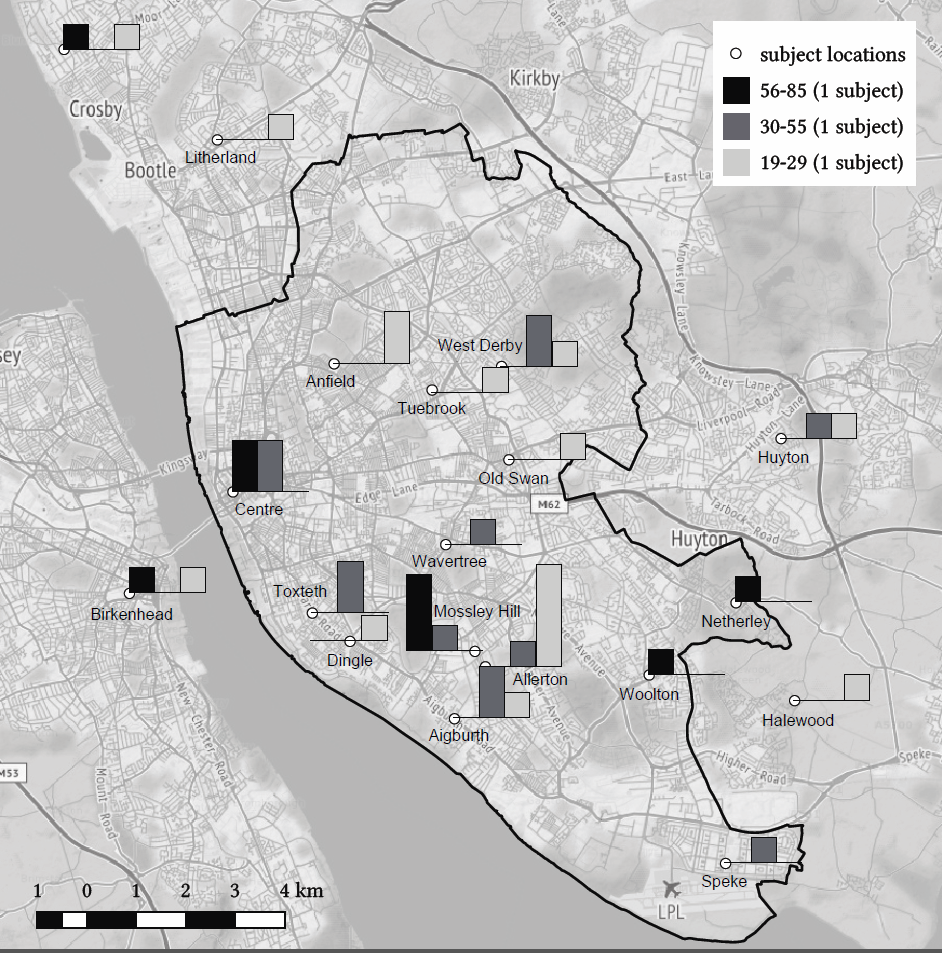
\includegraphics[width=0.8\textwidth]{figures/liverpool-participant-map.png}
		\caption{Geographical distribution of interview subjects}\label{fig.map.participants}
	\end{figure}

The study was not restricted to people from within the Liverpool Council boundaries (black line in the map), but also included areas which are administered by other local councils (Sefton, Knowsley, \isi{Wirral}) and which are, therefore, ``technically not Liverpool'' as a number of subjects put it. This is indeed, however, more of a technicality since we are talking about a contiguously built up area -- just like in most other urban agglomerations. It is clear that invisible lines (sometimes separating one side of a street from the other) can still be important for people's \isi{identity}, but all of the participants in this study self-identified as Liverpudlian\is{identity}s or Scouser\is{identity}s. This also held for the two subjects who were actually living on the \isi{Wirral} and who had both been born in Liverpool (and in one case also lived half her life within Liverpool city boundaries). Generally speaking, people in urban areas often move around quite a bit and this might be especially true for Liverpool where many people from inner city areas were actually relocated (sometimes very reluctantly so) to new housing estates on the outskirts of the city during the slum clearances of the 50s and 60s. This is indeed what many of the older participants experienced themselves. For these reasons it was deemed unjustified to restrict the pool of subjects to those living within Liverpool city boundaries only.

	\section{Transcription}\label{sec.prod_method.transcription}

All interviews were transcribed orthographically in Praat \parencite{praat} by the author.
Since the transcriptions' sole purpose was to serve as input for automatic measuring (cf. \sectref{sec.prod_method.measuring}), pauses, \isi{intonation}, stress, etc. were not marked in the transcripts.
Questions and other utterances by the interviewer were \rephrase{equally}{also } ignored.
On separate tiers of the Praat TextGrid, speaking style (word ``list'', ``reading'' (passage), ``free'' (speech), and (accent) ``imitation\is{accent performance}'') and topic (``childhood'', ``Manchester'', ``\isi{identity}'' etc.) coded, followed by a third one where the participant's speech was segmented into chunks and transcribed.
Words containing test tokens and the individual variables themselves were marked on individual tiers called ``word'' and ``variable'' respectively.
Finally, a sixth tier called ``aspiration'' was used to mark relevant parts of the consonantal variables (cf. \sectref{sec.prod_method.con}).
\figref{fig.textgrid.ex} provides an extract from a TextGrid (zoomed to word level) for purposes of illustration.

	\begin{figure}
		
			
			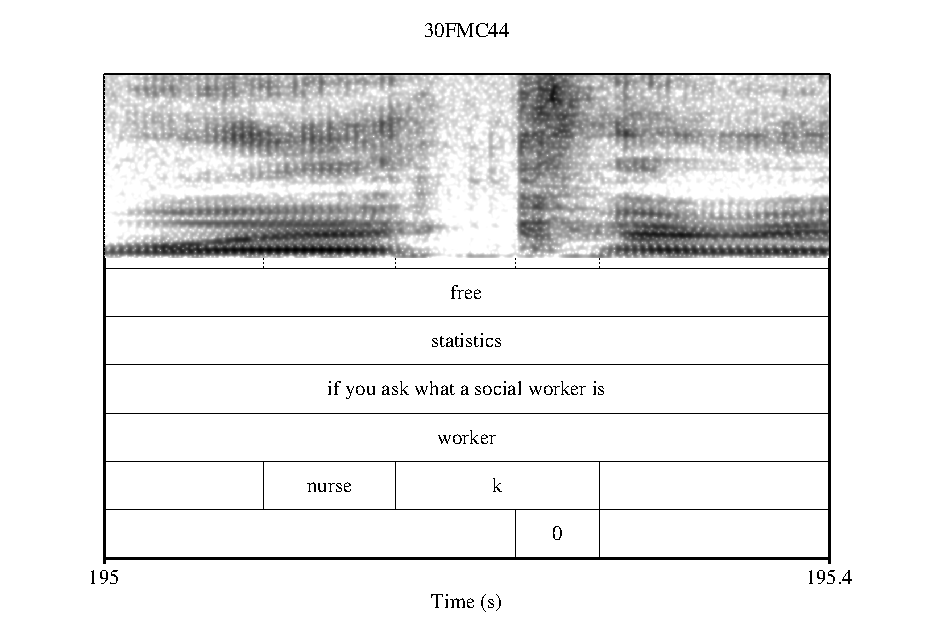
\includegraphics[width=0.75\textwidth]{figures/TextGrid_screenshot}
		\caption{Extract of Praat TextGrid (subject 30FMC44)}
		\label{fig.textgrid.ex}
	\end{figure}

	\section{Measuring}\label{sec.prod_method.measuring}

		\subsection{Consonants}\label{sec.prod_method.con}

The two consonantal variables were analysed both acoustically and auditorily.
The method for acoustic measuring of /k/ was heavily inspired by the one used in \citealt{sangster2001} to investigate lenition of alveolar stops. Phonetic plosives have a period of silence, or closure, followed by a burst and friction. For affricates, there is the same silence, but more friction than for plosives, and fricatives have either a very short period of silence or none at all and consist (almost) entirely of friction. 

Beginning and end of the friction phase were marked in a Praat TextGrid for every /k/. 
A script written by the author was then used to automatically measure the duration of these segments as well as the total durations of the plosives (i.e. including the closure phase).
/k/ tokens without any friction phase were registered as `unreleased' (and ignored in the analysis).
Next, what \citeauthor{sangster2001} calls `the proportional duration of friction' (\isi{PDF}) was calculated by dividing the duration of the friction phase by the total duration of the plosive. The result is a figure between 0 (or 0\%) and 1 (100\%), with lower values for more plosive-like realisations and higher values for sounds that are phonetically speaking affricates or fricatives.

The same technique was applied to /ŋ(g)/.
This decision might seem strange at first, because the realisational options of /ŋ(g)/ do not seem to be readily comparable to those of /k/.
Closer examination, however, reveals that the standard realisation as a nasal [ŋ] involves complete oral closure -- just as with [k] -- and that for the typical Scouse realisation as [ŋg] this closure phase is followed by a release burst / friction.
While the friction of [ŋg] will never be as long as that of a /k/ realised as a fricative, the \isi{PDF} values will mean the same thing for velar nasal plus as they do for /k/: lower values (no or little friction \(\rightarrow\) [ŋ]) indicate a standard-like realisation and higher scores (presence of friction \(\rightarrow\) [ŋg]) mark non-standard, Scouse variants.
Alveolar variants of /ŋ(g)/ were coded as ``in'' and later removed for the quantitative analyses for two reasons.
First, [n] is a non-standard variant that is not limited to Liverpool or even a clearly bounded region, but one that is used in all varieties of English English and many others as well.
It is also rather salient\is{salience} and commented on\is{overt commentary} by many non-linguists as \enquote*{g-dropping}.
However, in order to assess the impact of \isi{salience}, particularly in perception, this study required a local/regional feature with little or no \isi{salience}, to compare to the highly salient\is{salience} and local /k/ lenition.
Alveolar variants of the <ng> cluster fulfil neither criterion, while [ŋg] realisations tick both boxes.
The second reason concerns the method of measurement.
Realising <ng> as [n] by definition excludes the presence of even a hint of a plosive, so the \isi{PDF} measurement outlined above is not applicable.
The difference between [ŋ] and [ŋg] (or the devoiced\is{devoicing} variant [ŋk]), on the other hand, exhibits the same kind of gradualness and, as explained above, can be measured in the same way as /k/ lenition.
This parallelism is again crucial for the perception experiment, because it means the stimuli for /k/ and /ŋ(g)/ could be manipulated in a way that was phonetically similar (and thus not a confound).
Since linking up data from production and perception is a major interest of this study, the focus in the production part was also exclusively on the [ŋ]-[ŋg] distinction.
\figref{fig.automatic.consonants} shows two examples and their respective marking in the TextGrid.

	\begin{figure}
		
		\begin{subfigure}{0.75\textwidth}
			
			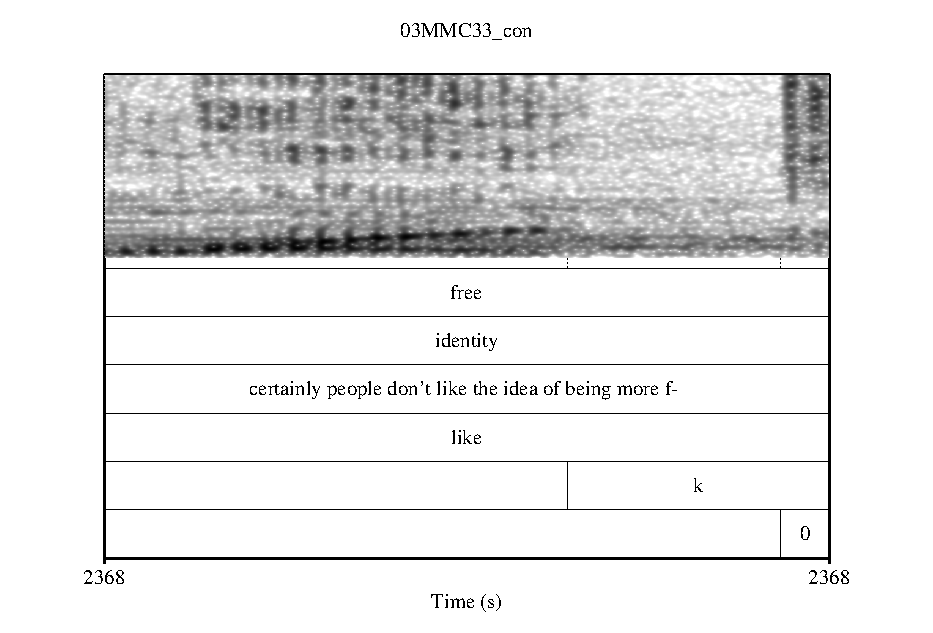
\includegraphics[width=\textwidth]{figures/like_plosive}
			\caption{plosive, PDF = 18.47\% (03MMC33)}
		\end{subfigure}
		\begin{subfigure}{0.75\textwidth}
			
			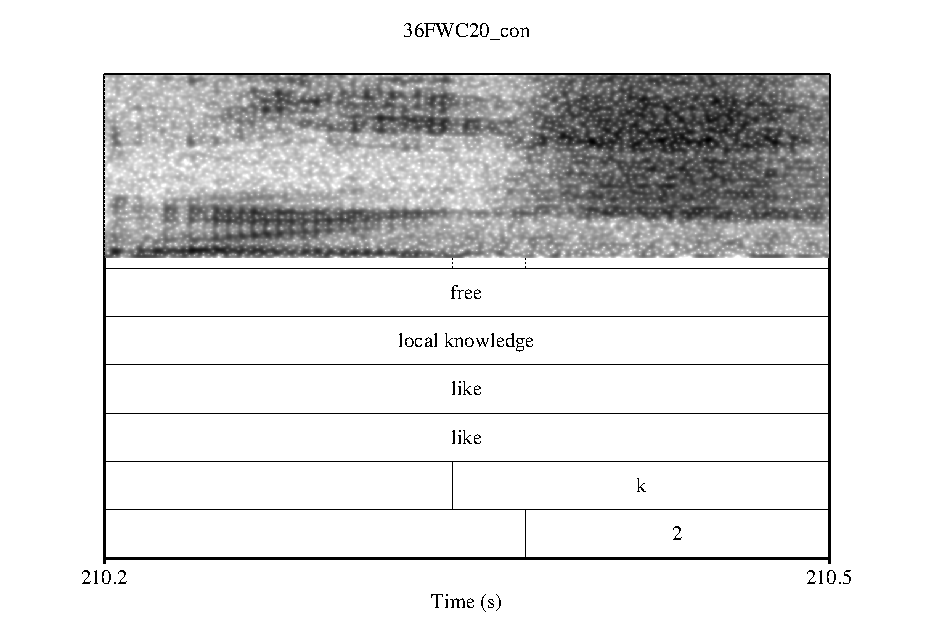
\includegraphics[width=\textwidth]{figures/like_fricative}
			\caption{fricative, PDF = 81.84\% (36FWC20)}
		\end{subfigure}
		\caption{Spectrograms of /k/ (zoomed to word level)}
		\label{fig.automatic.consonants}
	\end{figure}

	\newpage 
This very precise method of acoustically measuring /k/ and velar nasal plus requires high quality recordings with little to no background noise.
As it was unclear at the beginning whether all interviews fulfilled these criteria, the data were also analysed auditorily by the author. 
Coding was `0' (plosive), `1' (affricate), and `2' (fricative) for /k/, and `0' (nasal) and `1' (nasal plus burst) for /ŋ(g)/.
It turned out that all interviews included in this project actually did permit an analysis based on the more precise \citeauthor{sangster2001} method, so the auditory coding was not used in the analysis in the end.
It is, however, still accessible for future research.

		\subsection{Vowels}\label{sec.prod_method.vow}
		
For the measurement of the first two (later three) vowel formants (\textsc{nurse}, \textsc{square}, and \textsc{happy}) a Praat script\footnote{Generously made available by Mietta Lennes -- \url{http://www.helsinki.fi/~lennes/praat-scripts/}, last accessed 2013-01-29 -- and modified by the author.} was used to automatise data collection.
\textsc{nurse} and \textsc{square} were measured first by hand and then in an automated way by the script for the first three (male) subjects.
Paired t-tests were then administered to make sure the automated measurements were reliable. Neither test ([t(545) = -0.975, p = 0.330] for F1 and [t(545) = 1.768, p = 0.078] for F2) found a significant difference between hand and automated measurements, although there was a trend for the F2 values.
However, the mean difference between hand and automated measurements for F2 was a mere 2.15 Hz.
Scatterplots furthermore show a near-perfect correlation of hand and automated measurements, which is why the script was deemed reliable and all formant measurements used in the final analysis were taken automatically only.
Clear mismeasurements were later removed from the dataset.

		\begin{figure}
			
				\begin{subfigure}[b]{0.45\textwidth}
					
					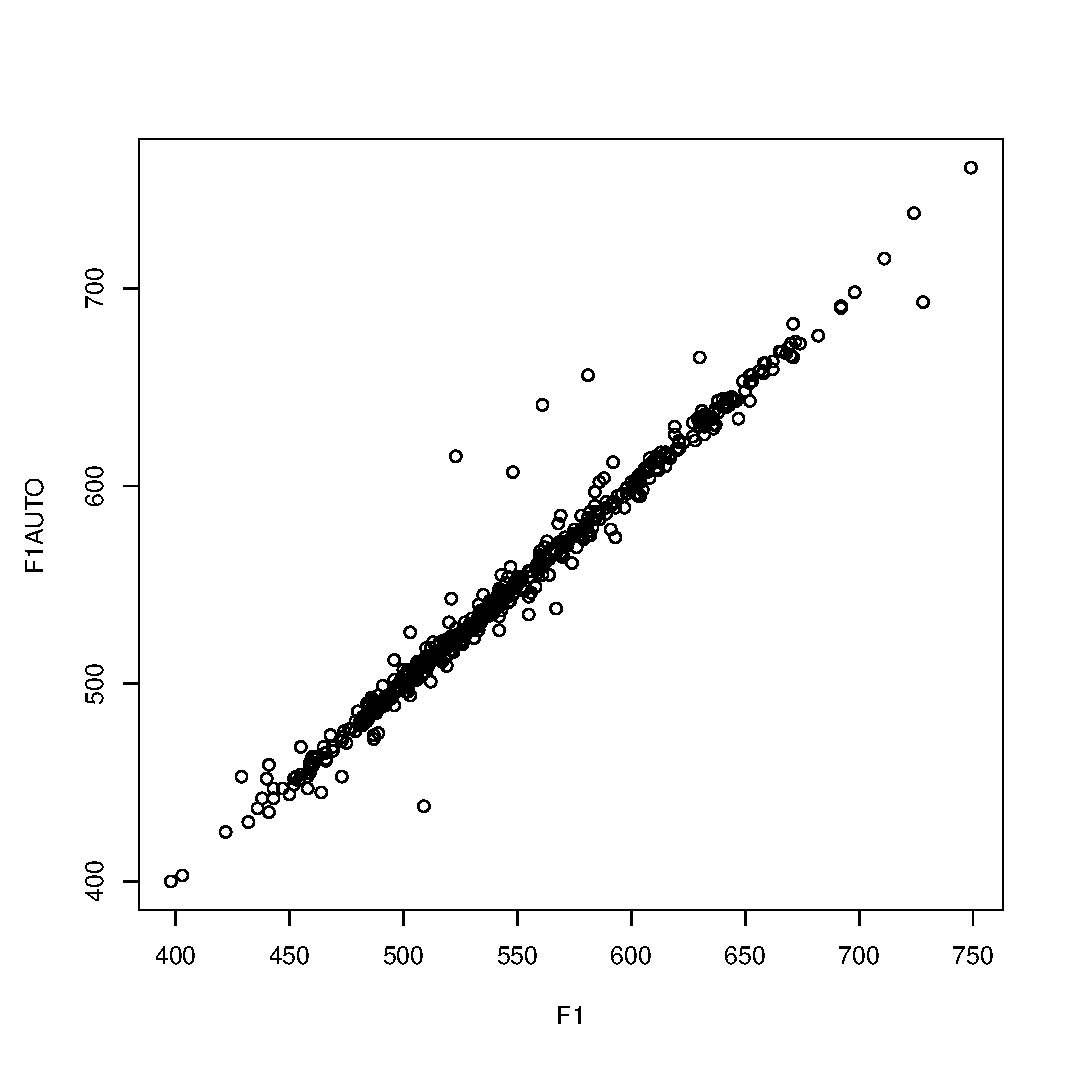
\includegraphics[width=\textwidth]{figures/F1F1AUTO}
					\caption{F1 measurements}
				\end{subfigure}
				\begin{subfigure}[b]{0.45\textwidth}
					
					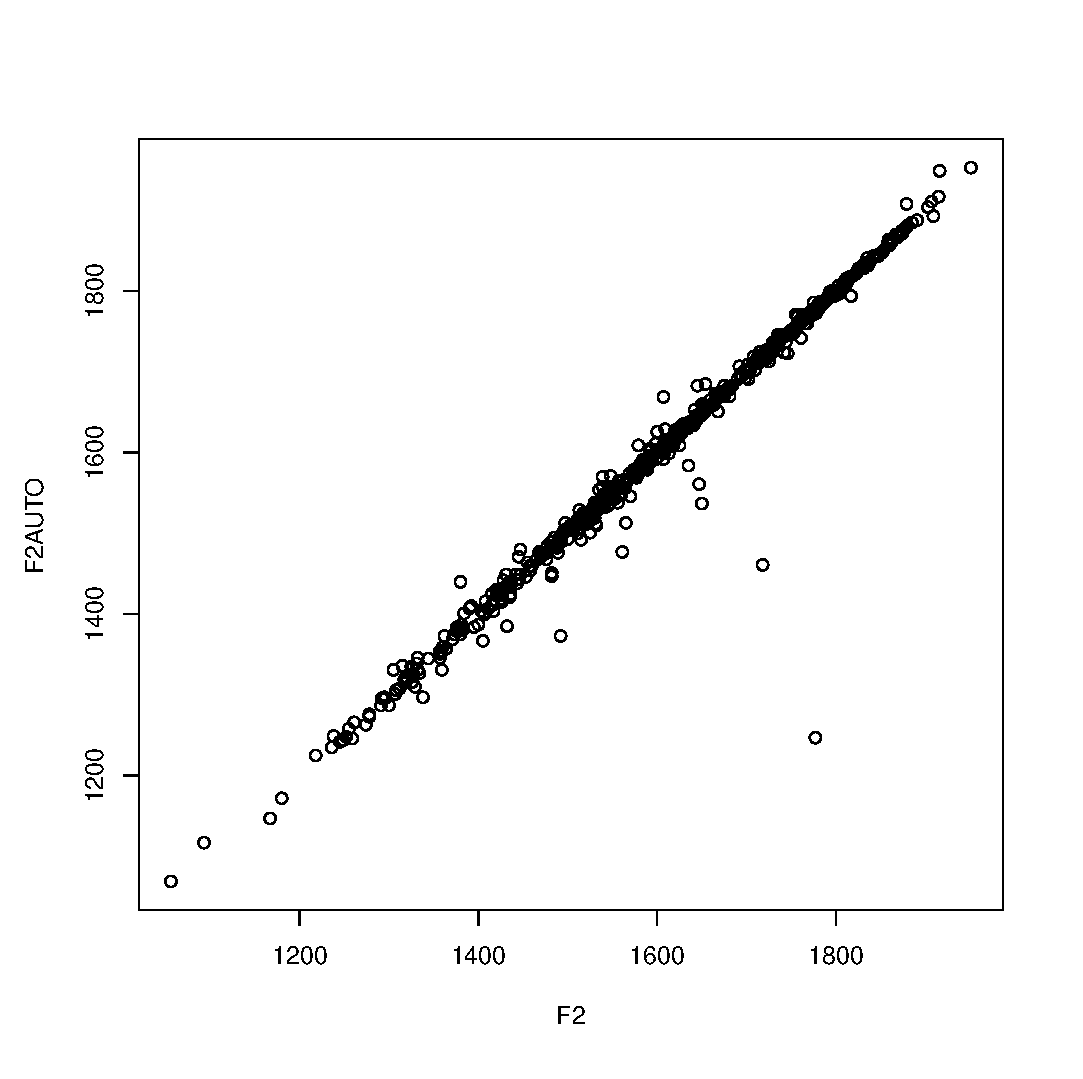
\includegraphics[width=\textwidth]{figures/F2F2AUTO}
					\caption{F2 measurements}
				\end{subfigure}
			\caption[Manual vs. automatic measurements (\textsc{nurse} and \textsc{square})]{Manual (x-axis) vs. automatic (y-axis) measurements of \textsc{nurse} and \textsc{square}}\label{fig.automatic.measurements}
		\end{figure}

The script took as input pairs of sound files and TextGrids.
It then went through each TextGrid and looked for vowel labels in the variable tier.
When it found a relevant label it noted the start and end of the segment and measured F1, F2, and F3 at midpoint of the vowel.
It then extracted information about the style, topic, carrier word, and the larger context it appeared in from the other tiers and saved all these data into a textfile.
F3 was measured because it was needed for one of the \isi{normalisation} algorithms that were later applied to the raw measurements (cf. \sectref{sec.prod_method.norm}).
In addition to the three vocalic test variables happ\textsc{y}, \textsc{nurse}, and \textsc{square} (of which all instances were included), between 10 and 25 tokens of \textsc{fleece} and \textsc{trap} per subject were also measured.
These were taken from the reading passage and word list sections of the interviews since these contexts were considered most likely to produce the most `extreme' realisations (in terms of the periphery of speakers' vowel spaces).
Observations of \textsc{trap} were used exclusively as input for \isi{normalisation} and for comparison of the algorithms (again, cf. \sectref{sec.prod_method.norm}).
\textsc{fleece} measurements were additionally included in the calculation of \isi{Pillai} scores for happ\textsc{y} (cf. \sectref{sec.prod.res.vow.happy.pil}).

\subsection{Normalisation}\label{sec.prod_method.norm}

It is a well known fact among phoneticians and phonologists that there is a huge amount of variation in the acoustic signal that is not due to linguistic or sociolingustic, but rather purely physiological reasons.
Even multiple realisations of one and the same phonological sound chain produced by a single speaker in the same style will all be slightly different from one another.
In addition to these intra-speaker differences, there are also inter-speaker ones.
The most pronounced differences in this area are due to vocal tract length.
The length of the vocal tract correlates inversely with vowel formant values.
On average, therefore, children (with the shortest vocal tracts) have higher formants than women, who in turn have higher formants than men for one and the same phonological vowel.
The potential effect of vocal tract maturation, i.e. changes to length and shape of the vocal tract over the course of an individuals lifetime, further complicates matters \parencite[cf.][440--441]{harrington2006}.

It is therefore not possible (or at least not advisable) to directly compare, for instance, women's and men's raw formant values, or those of younger and older speakers.
This is where \isi{normalisation} comes in.
According to several articles on the matter \parencite[cf., for example,][]{fabriciusetal2009,clopper2009,disner1980,kendallthomas2014,thomas2002}, \isi{normalisation} should ideally achieve four different goals:
\begin{enumerate}
	\item \label{enum.norm.phys}elimination of differences that are due to physiological reasons
	\item \label{enum.norm.soc}preservation of differences that are (socio-)linguistic in nature
	\item \label{enum.norm.phon}preservation (or improvement) of phoneme distinctions
	\item \label{enum.norm.cog}modelling the process that allows listeners to assign realisations from different speakers to one and the same phoneme
\end{enumerate}
The author is well aware of the irony involved here.
This study is, after all, set in an \isi{exemplar} framework which suggests that listeners do \emph{not} normalise\is{normalisation} acoustic input, at least not in the same way and to the same degree as is assumed in most other phonological theories.
This is most relevant with respect to point \ref{enum.norm.cog} in the enumeration above. Sociolinguists, however, usually largely ignore this aspect and focus more on points \ref{enum.norm.phys} and \ref{enum.norm.soc} \parencites(cf.)()[1430]{clopper2009}[414--415]{fabriciusetal2009}{kendallthomas2014}, and the present study is no exception.
By applying a \isi{normalisation} algorithm to the data I do not mean to suggest that this procedure mirrors or approximates what happens in listeners' brains.
Rather, it is simply the only option one has if the goal is to compare production data of men and women (or those of younger and older speakers) to each other instead of treating them separately.

Normalisation methods are generally categorised with respect to two dimensions: vowel-intrinsic vs. vowel-extrinsic and speaker-intrinsic vs. speaker-ex\-trin\-sic \parencite[cf.][]{kendallthomas2014}.
Vowel-intrinsic algorithms extract all data necessary for \isi{normalisation} from the individual token.
Often these methods use F0 and/or F3 to estimate vocal tract length.
Vowel-extrinsic algorithms include formant measurements from more than one vowel in their formulas and achieve \isi{normalisation} with the help of means over several (often all) measured vowels.
Speaker-intrinsic methods differ from speaker-extrinsic ones in that the former perform \isi{normalisation} for each speaker individually (i.e. only taking into account vowels produced by that speaker), whereas the latter include some sort of inter-speaker mean in their calculations (cf., for example, \citegen{labovetal2006} \emph{grand mean}).

A number of algorithms have been proposed over the years, and the question which of those fares best in achieving the goals spelled out above has generated a series of investigations \parencites(among others:)(){hindle1978}{disner1980}{adanketal2004}.
Generally speaking, ``vowel-extrinsic methods tend to perform better overall (\ldots) for vowel space normalization across talkers'', and ``vowel-intrinsic methods are appealing as perceptually plausible models of human speech processing'' \parencite[1440]{clopper2009}.
For this reason, two different \isi{normalisation} methods were tested in this study, a vowel-intrinsic and a vowel-extrinsic one (both of them speaker-intrinsic).
Both \isi{normalisation}s were applied to the raw data using the NORM package for R \parencite{kendallthomas2014}.
The first, Bark difference, was devised by \textcite{syrdalgopal1986}, and is a vowel-intrinsic method.
Formants are, first of all, transformed into -- perceptually ``more accurate'' \parencite[1431--1432]{clopper2009} -- Bark values using the formula taken from \textcite{traunmueller1990}:

\begin{equation}
	Z_{i} = \frac{26.81}{1 + \frac{1960}{F_{i}}} - 0.53
\end{equation}

Where \(F_{i}\) is the raw value of a given formant. The Bark rescaled values \(Z_{1}\) and \(Z_{2}\) are then substracted from \(Z_{3}\) to arrive at normalise\is{normalisation}d measures of height and frontness respectively. \citeauthor{syrdalgopal1986} originally used Bark-converted F0 instead of F3 for the height dimension, but \textcite{kendallthomas2014} argue that a number of things, for instance ``[i]ntonation, tone, and consonantal influences affect F0'' and consider it preferable to use Bark-converted F3 for both the back-front and the high-low dimension.

The most popular vowel-extrinsic \isi{normalisation} method among sociolinguists is probably \textcite{lobanov1971}.
This is unsurprising given the fact that it has frequently been found to be (one of) the most efficient algorithm(s) in reducing physiological and preserving sociolinguistic variation \parencite[cf.][1440]{clopper2009}.
The main drawback of \citeauthor{lobanov1971} -- and many other vowel-extrinsic algorithms -- is that it works best when \emph{all} vowels of a system are measured.
Constraints of time and resources made this endeavour impractical for the present study.
The choice fell on \textcite{wattfabricius2002} in its modified version \parencite{fabriciusetal2009} instead, a method which is ``conceptually similar'' and deemed ``also successful'' \parencite[1440]{clopper2009}.

\textcite{wattfabricius2002} assume a triangular vowel space with the `corner' vowels \([i]\), \([a]\), and \([u']\).
In RP (for which the algorithm was originally designed), these would correspond to \textsc{fleece}, \textsc{trap}, and \textsc{goose}, but
the NORM package automatically chooses the highest/most fronted and the most open vowel available in the sample as \([i]\) and \([a]\), irrespective of their labels.
Obviously, \([i]\) and \([a]\) should be relatively stable in the variety under scrutiny \parencite[cf.][163]{wattfabricius2002}.
Since I am not aware of any evidence that suggests this is \emph{not} true for \textsc{fleece} and \textsc{trap} in Scouse, these two were used as corners in this study.
From these benchmark vowels, a `centroid' S or ``centre of gravity'' \parencite[164]{wattfabricius2002} is then computed as follows:
\begin{equation}
	S(F_{n}) = \frac{[i]F_{n} + [a]F_{n} + [u']F_{n}}{3}
\end{equation}
Where \(F_{n}\) is a mean raw formant value of the corner vowels \([i]\), \([a]\), and \([u']\). The centroid value \(S(F_{n})\) is computed separately for each formant, and normalise\is{normalisation}d values are then expressed as the ratio of the raw measurement to the corresponding centroid: \(\frac{F_{n}}{S(F_{n})}\).
Note that \([u']\) is not measured, but derived from \([i]\), assuming that \([u']F_{1}\) = \([u']F_{2}\) = \([i]F_{1}\).
As a result, only \textsc{fleece} and \textsc{trap} have to be measured.
To counter potential skewing due to the fact that \textsc{trap} might not be exactly halfway between \textsc{fleece} and \textsc{goose} with respect to frontness, \([a]F_{2}\) is also derived instead of measured in the modified version of the algorithm employed in this study \parencites(cf.)()[420--421]{fabriciusetal2009}{kendallthomas2014}.

				\begin{figure}
					
					\begin{subfigure}{.49\textwidth}
						
						\resizebox{\linewidth}{!}{% Created by tikzDevice version 0.10.1 on 2017-03-15 16:22:39
% !TEX encoding = UTF-8 Unicode
\begin{tikzpicture}[x=1pt,y=1pt]
\definecolor{fillColor}{RGB}{255,255,255}
\path[use as bounding box,fill=fillColor,fill opacity=0.00] (0,0) rectangle (202.36,202.36);
\begin{scope}
\path[clip] (  0.00,  0.00) rectangle (202.36,202.36);
\definecolor{drawColor}{RGB}{255,255,255}
\definecolor{fillColor}{RGB}{255,255,255}

\path[draw=drawColor,line width= 0.6pt,line join=round,line cap=round,fill=fillColor] (  0.00,  0.00) rectangle (202.36,202.36);
\end{scope}
\begin{scope}
\path[clip] ( 45.67, 33.48) rectangle (196.36,196.36);
\definecolor{fillColor}{RGB}{255,255,255}

\path[fill=fillColor] ( 45.67, 33.48) rectangle (196.36,196.36);
\definecolor{drawColor}{gray}{0.98}

\path[draw=drawColor,line width= 0.6pt,line join=round] ( 45.67,179.73) --
	(196.36,179.73);

\path[draw=drawColor,line width= 0.6pt,line join=round] ( 45.67,140.06) --
	(196.36,140.06);

\path[draw=drawColor,line width= 0.6pt,line join=round] ( 45.67,100.39) --
	(196.36,100.39);

\path[draw=drawColor,line width= 0.6pt,line join=round] ( 45.67, 60.72) --
	(196.36, 60.72);

\path[draw=drawColor,line width= 0.6pt,line join=round] (181.85, 33.48) --
	(181.85,196.36);

\path[draw=drawColor,line width= 0.6pt,line join=round] (140.67, 33.48) --
	(140.67,196.36);

\path[draw=drawColor,line width= 0.6pt,line join=round] ( 99.49, 33.48) --
	( 99.49,196.36);
\definecolor{drawColor}{gray}{0.90}

\path[draw=drawColor,line width= 0.2pt,line join=round] ( 45.67,159.89) --
	(196.36,159.89);

\path[draw=drawColor,line width= 0.2pt,line join=round] ( 45.67,120.22) --
	(196.36,120.22);

\path[draw=drawColor,line width= 0.2pt,line join=round] ( 45.67, 80.55) --
	(196.36, 80.55);

\path[draw=drawColor,line width= 0.2pt,line join=round] ( 45.67, 40.88) --
	(196.36, 40.88);

\path[draw=drawColor,line width= 0.2pt,line join=round] (161.26, 33.48) --
	(161.26,196.36);

\path[draw=drawColor,line width= 0.2pt,line join=round] (120.08, 33.48) --
	(120.08,196.36);

\path[draw=drawColor,line width= 0.2pt,line join=round] ( 78.90, 33.48) --
	( 78.90,196.36);
\definecolor{drawColor}{RGB}{0,0,0}

\node[text=drawColor,anchor=base,inner sep=0pt, outer sep=0pt, scale=  0.71] at (102.35,157.97) {FLEECE};

\node[text=drawColor,anchor=base,inner sep=0pt, outer sep=0pt, scale=  0.71] at (108.87,152.81) {HAPPY};

\node[text=drawColor,anchor=base,inner sep=0pt, outer sep=0pt, scale=  0.71] at (132.29,123.92) {NURSE};

\node[text=drawColor,anchor=base,inner sep=0pt, outer sep=0pt, scale=  0.71] at (127.12,123.10) {SQUARE};

\node[text=drawColor,anchor=base,inner sep=0pt, outer sep=0pt, scale=  0.71] at (157.86, 82.93) {TRAP};

\path[draw=drawColor,line width= 0.6pt,line join=round] (152.45,159.68) --
	(152.07,162.88) --
	(150.94,166.06) --
	(149.07,169.19) --
	(146.50,172.20) --
	(143.26,175.06) --
	(139.40,177.72) --
	(134.98,180.15) --
	(130.06,182.29) --
	(124.73,184.13) --
	(119.06,185.63) --
	(113.14,186.77) --
	(107.05,187.54) --
	(100.90,187.92) --
	( 94.76,187.91) --
	( 88.75,187.50) --
	( 82.94,186.70) --
	( 77.43,185.53) --
	( 72.30,184.01) --
	( 67.62,182.14) --
	( 63.47,179.98) --
	( 59.91,177.54) --
	( 57.00,174.86) --
	( 54.77,171.99) --
	( 53.27,168.96) --
	( 52.52,165.83) --
	( 52.52,162.64) --
	( 53.27,159.44) --
	( 54.77,156.28) --
	( 57.00,153.21) --
	( 59.91,150.26) --
	( 63.47,147.50) --
	( 67.62,144.95) --
	( 72.30,142.66) --
	( 77.43,140.67) --
	( 82.94,138.99) --
	( 88.75,137.67) --
	( 94.76,136.71) --
	(100.90,136.14) --
	(107.05,135.96) --
	(113.14,136.17) --
	(119.06,136.77) --
	(124.73,137.75) --
	(130.06,139.11) --
	(134.98,140.80) --
	(139.40,142.82) --
	(143.26,145.13) --
	(146.50,147.69) --
	(149.07,150.47) --
	(150.94,153.43) --
	(152.07,156.51) --
	(152.45,159.68);

\path[draw=drawColor,line width= 0.6pt,line join=round] (156.17,153.56) --
	(155.83,157.52) --
	(154.79,161.47) --
	(153.07,165.34) --
	(150.71,169.09) --
	(147.73,172.65) --
	(144.18,175.97) --
	(140.12,179.00) --
	(135.60,181.70) --
	(130.70,184.02) --
	(125.49,185.92) --
	(120.05,187.39) --
	(114.46,188.39) --
	(108.80,188.91) --
	(103.17,188.95) --
	( 97.64,188.50) --
	( 92.31,187.57) --
	( 87.24,186.18) --
	( 82.53,184.34) --
	( 78.23,182.08) --
	( 74.42,179.44) --
	( 71.15,176.46) --
	( 68.47,173.18) --
	( 66.43,169.65) --
	( 65.05,165.93) --
	( 64.35,162.07) --
	( 64.35,158.13) --
	( 65.05,154.17) --
	( 66.43,150.25) --
	( 68.47,146.44) --
	( 71.15,142.77) --
	( 74.42,139.33) --
	( 78.23,136.14) --
	( 82.53,133.28) --
	( 87.24,130.76) --
	( 92.31,128.65) --
	( 97.64,126.96) --
	(103.17,125.72) --
	(108.80,124.96) --
	(114.46,124.68) --
	(120.05,124.88) --
	(125.49,125.57) --
	(130.70,126.74) --
	(135.60,128.36) --
	(140.12,130.41) --
	(144.18,132.86) --
	(147.73,135.68) --
	(150.71,138.82) --
	(153.07,142.23) --
	(154.79,145.86) --
	(155.83,149.66) --
	(156.17,153.56);

\path[draw=drawColor,line width= 0.6pt,line join=round] (179.87,131.05) --
	(179.52,134.68) --
	(178.48,138.20) --
	(176.75,141.55) --
	(174.37,144.69) --
	(171.38,147.55) --
	(167.81,150.11) --
	(163.72,152.33) --
	(159.18,154.16) --
	(154.25,155.58) --
	(149.01,156.57) --
	(143.54,157.11) --
	(137.92,157.20) --
	(132.23,156.84) --
	(126.56,156.03) --
	(121.00,154.77) --
	(115.64,153.10) --
	(110.54,151.04) --
	(105.80,148.62) --
	(101.48,145.87) --
	( 97.64,142.83) --
	( 94.36,139.56) --
	( 91.66,136.10) --
	( 89.61,132.51) --
	( 88.22,128.83) --
	( 87.52,125.13) --
	( 87.52,121.46) --
	( 88.22,117.88) --
	( 89.61,114.44) --
	( 91.66,111.19) --
	( 94.36,108.18) --
	( 97.64,105.46) --
	(101.48,103.07) --
	(105.80,101.05) --
	(110.54, 99.42) --
	(115.64, 98.21) --
	(121.00, 97.44) --
	(126.56, 97.12) --
	(132.23, 97.26) --
	(137.92, 97.85) --
	(143.54, 98.88) --
	(149.01,100.35) --
	(154.25,102.22) --
	(159.18,104.46) --
	(163.72,107.06) --
	(167.81,109.95) --
	(171.38,113.11) --
	(174.37,116.48) --
	(176.75,120.02) --
	(178.48,123.66) --
	(179.52,127.35) --
	(179.87,131.05);

\path[draw=drawColor,line width= 0.6pt,line join=round] (171.18,128.67) --
	(170.86,132.23) --
	(169.89,135.70) --
	(168.29,139.03) --
	(166.09,142.18) --
	(163.32,145.09) --
	(160.01,147.72) --
	(156.23,150.03) --
	(152.03,151.98) --
	(147.46,153.55) --
	(142.61,154.71) --
	(137.54,155.44) --
	(132.34,155.73) --
	(127.07,155.58) --
	(121.83,155.00) --
	(116.68,153.98) --
	(111.71,152.54) --
	(106.99,150.71) --
	(102.60,148.52) --
	( 98.60,145.99) --
	( 95.05,143.17) --
	( 92.01,140.10) --
	( 89.51,136.82) --
	( 87.61,133.38) --
	( 86.32,129.85) --
	( 85.68,126.26) --
	( 85.68,122.68) --
	( 86.32,119.15) --
	( 87.61,115.74) --
	( 89.51,112.50) --
	( 92.01,109.46) --
	( 95.05,106.69) --
	( 98.60,104.21) --
	(102.60,102.08) --
	(106.99,100.32) --
	(111.71, 98.95) --
	(116.68, 98.00) --
	(121.83, 97.49) --
	(127.07, 97.42) --
	(132.34, 97.79) --
	(137.54, 98.59) --
	(142.61, 99.82) --
	(147.46,101.46) --
	(152.03,103.47) --
	(156.23,105.84) --
	(160.01,108.51) --
	(163.32,111.47) --
	(166.09,114.65) --
	(168.29,118.01) --
	(169.89,121.50) --
	(170.86,125.07) --
	(171.18,128.67);

\path[draw=drawColor,line width= 0.6pt,line join=round] (189.51, 90.01) --
	(189.27, 95.69) --
	(188.57,101.23) --
	(187.41,106.57) --
	(185.81,111.61) --
	(183.80,116.28) --
	(181.40,120.52) --
	(178.66,124.25) --
	(175.61,127.42) --
	(172.30,129.98) --
	(168.78,131.89) --
	(165.11,133.13) --
	(161.33,133.67) --
	(157.51,133.51) --
	(153.70,132.65) --
	(149.97,131.10) --
	(146.37,128.89) --
	(142.94,126.04) --
	(139.76,122.61) --
	(136.86,118.65) --
	(134.28,114.20) --
	(132.07,109.35) --
	(130.27,104.17) --
	(128.88, 98.73) --
	(127.95, 93.11) --
	(127.48, 87.41) --
	(127.48, 81.70) --
	(127.95, 76.08) --
	(128.88, 70.63) --
	(130.27, 65.43) --
	(132.07, 60.57) --
	(134.28, 56.10) --
	(136.86, 52.11) --
	(139.76, 48.66) --
	(142.94, 45.79) --
	(146.37, 43.55) --
	(149.97, 41.97) --
	(153.70, 41.07) --
	(157.51, 40.88) --
	(161.33, 41.39) --
	(165.11, 42.60) --
	(168.78, 44.49) --
	(172.30, 47.02) --
	(175.61, 50.16) --
	(178.66, 53.87) --
	(181.40, 58.08) --
	(183.80, 62.74) --
	(185.81, 67.77) --
	(187.41, 73.09) --
	(188.57, 78.63) --
	(189.27, 84.30) --
	(189.51, 90.01);
\definecolor{drawColor}{gray}{0.50}

\path[draw=drawColor,line width= 0.6pt,line join=round,line cap=round] ( 45.67, 33.48) rectangle (196.36,196.36);
\end{scope}
\begin{scope}
\path[clip] (  0.00,  0.00) rectangle (202.36,202.36);
\definecolor{drawColor}{RGB}{0,0,0}

\node[text=drawColor,anchor=base east,inner sep=0pt, outer sep=0pt, scale=  0.80] at ( 40.27,156.59) {400};

\node[text=drawColor,anchor=base east,inner sep=0pt, outer sep=0pt, scale=  0.80] at ( 40.27,116.92) {600};

\node[text=drawColor,anchor=base east,inner sep=0pt, outer sep=0pt, scale=  0.80] at ( 40.27, 77.25) {800};

\node[text=drawColor,anchor=base east,inner sep=0pt, outer sep=0pt, scale=  0.80] at ( 40.27, 37.58) {1000};
\end{scope}
\begin{scope}
\path[clip] (  0.00,  0.00) rectangle (202.36,202.36);
\definecolor{drawColor}{RGB}{0,0,0}

\path[draw=drawColor,line width= 0.6pt,line join=round] ( 42.67,159.89) --
	( 45.67,159.89);

\path[draw=drawColor,line width= 0.6pt,line join=round] ( 42.67,120.22) --
	( 45.67,120.22);

\path[draw=drawColor,line width= 0.6pt,line join=round] ( 42.67, 80.55) --
	( 45.67, 80.55);

\path[draw=drawColor,line width= 0.6pt,line join=round] ( 42.67, 40.88) --
	( 45.67, 40.88);
\end{scope}
\begin{scope}
\path[clip] (  0.00,  0.00) rectangle (202.36,202.36);
\definecolor{drawColor}{RGB}{0,0,0}

\path[draw=drawColor,line width= 0.6pt,line join=round] (161.26, 30.48) --
	(161.26, 33.48);

\path[draw=drawColor,line width= 0.6pt,line join=round] (120.08, 30.48) --
	(120.08, 33.48);

\path[draw=drawColor,line width= 0.6pt,line join=round] ( 78.90, 30.48) --
	( 78.90, 33.48);
\end{scope}
\begin{scope}
\path[clip] (  0.00,  0.00) rectangle (202.36,202.36);
\definecolor{drawColor}{RGB}{0,0,0}

\node[text=drawColor,anchor=base,inner sep=0pt, outer sep=0pt, scale=  0.80] at (161.26, 21.47) {1500};

\node[text=drawColor,anchor=base,inner sep=0pt, outer sep=0pt, scale=  0.80] at (120.08, 21.47) {2000};

\node[text=drawColor,anchor=base,inner sep=0pt, outer sep=0pt, scale=  0.80] at ( 78.90, 21.47) {2500};
\end{scope}
\begin{scope}
\path[clip] (  0.00,  0.00) rectangle (202.36,202.36);
\definecolor{drawColor}{RGB}{0,0,0}

\node[text=drawColor,anchor=base,inner sep=0pt, outer sep=0pt, scale=  1.00] at (121.01,  8.40) {F2};
\end{scope}
\begin{scope}
\path[clip] (  0.00,  0.00) rectangle (202.36,202.36);
\definecolor{drawColor}{RGB}{0,0,0}

\node[text=drawColor,rotate= 90.00,anchor=base,inner sep=0pt, outer sep=0pt, scale=  1.00] at ( 16.67,114.92) {F1};
\end{scope}
\end{tikzpicture}
}
						\caption{raw data}
						\label{fig.plot.scatter.raw}
					\end{subfigure}
					
					\begin{subfigure}{.49\textwidth}
						
						\resizebox{\linewidth}{!}{% Created by tikzDevice version 0.10.1 on 2017-03-15 16:22:56
% !TEX encoding = UTF-8 Unicode
\begin{tikzpicture}[x=1pt,y=1pt]
\definecolor{fillColor}{RGB}{255,255,255}
\path[use as bounding box,fill=fillColor,fill opacity=0.00] (0,0) rectangle (202.36,202.36);
\begin{scope}
\path[clip] (  0.00,  0.00) rectangle (202.36,202.36);
\definecolor{drawColor}{RGB}{255,255,255}
\definecolor{fillColor}{RGB}{255,255,255}

\path[draw=drawColor,line width= 0.6pt,line join=round,line cap=round,fill=fillColor] (  0.00,  0.00) rectangle (202.36,202.36);
\end{scope}
\begin{scope}
\path[clip] ( 43.58, 33.48) rectangle (196.36,196.36);
\definecolor{fillColor}{RGB}{255,255,255}

\path[fill=fillColor] ( 43.58, 33.48) rectangle (196.36,196.36);
\definecolor{drawColor}{gray}{0.98}

\path[draw=drawColor,line width= 0.6pt,line join=round] ( 43.58, 60.42) --
	(196.36, 60.42);

\path[draw=drawColor,line width= 0.6pt,line join=round] ( 43.58,104.12) --
	(196.36,104.12);

\path[draw=drawColor,line width= 0.6pt,line join=round] ( 43.58,147.82) --
	(196.36,147.82);

\path[draw=drawColor,line width= 0.6pt,line join=round] ( 43.58,191.51) --
	(196.36,191.51);

\path[draw=drawColor,line width= 0.6pt,line join=round] ( 85.87, 33.48) --
	( 85.87,196.36);

\path[draw=drawColor,line width= 0.6pt,line join=round] (132.68, 33.48) --
	(132.68,196.36);

\path[draw=drawColor,line width= 0.6pt,line join=round] (179.49, 33.48) --
	(179.49,196.36);
\definecolor{drawColor}{gray}{0.90}

\path[draw=drawColor,line width= 0.2pt,line join=round] ( 43.58, 38.57) --
	(196.36, 38.57);

\path[draw=drawColor,line width= 0.2pt,line join=round] ( 43.58, 82.27) --
	(196.36, 82.27);

\path[draw=drawColor,line width= 0.2pt,line join=round] ( 43.58,125.97) --
	(196.36,125.97);

\path[draw=drawColor,line width= 0.2pt,line join=round] ( 43.58,169.67) --
	(196.36,169.67);

\path[draw=drawColor,line width= 0.2pt,line join=round] ( 62.47, 33.48) --
	( 62.47,196.36);

\path[draw=drawColor,line width= 0.2pt,line join=round] (109.28, 33.48) --
	(109.28,196.36);

\path[draw=drawColor,line width= 0.2pt,line join=round] (156.08, 33.48) --
	(156.08,196.36);
\definecolor{drawColor}{RGB}{0,0,0}

\node[text=drawColor,anchor=base,inner sep=0pt, outer sep=0pt, scale=  0.71] at (100.49,146.02) {FLEECE};

\node[text=drawColor,anchor=base,inner sep=0pt, outer sep=0pt, scale=  0.71] at (103.25,139.78) {HAPPY};

\node[text=drawColor,anchor=base,inner sep=0pt, outer sep=0pt, scale=  0.71] at (123.15,115.34) {NURSE};

\node[text=drawColor,anchor=base,inner sep=0pt, outer sep=0pt, scale=  0.71] at (117.45,114.60) {SQUARE};

\node[text=drawColor,anchor=base,inner sep=0pt, outer sep=0pt, scale=  0.71] at (137.43, 77.78) {TRAP};

\path[draw=drawColor,line width= 0.6pt,line join=round] (143.93,166.62) --
	(143.58,171.01) --
	(142.52,175.04) --
	(140.77,178.66) --
	(138.37,181.79) --
	(135.34,184.40) --
	(131.73,186.45) --
	(127.60,187.91) --
	(123.00,188.74) --
	(118.02,188.95) --
	(112.72,188.53) --
	(107.18,187.48) --
	(101.50,185.82) --
	( 95.74,183.57) --
	( 90.01,180.78) --
	( 84.39,177.47) --
	( 78.96,173.71) --
	( 73.81,169.54) --
	( 69.01,165.04) --
	( 64.64,160.27) --
	( 60.76,155.30) --
	( 57.44,150.21) --
	( 54.71,145.07) --
	( 52.63,139.96) --
	( 51.23,134.97) --
	( 50.52,130.16) --
	( 50.52,125.61) --
	( 51.23,121.39) --
	( 52.63,117.56) --
	( 54.71,114.18) --
	( 57.44,111.30) --
	( 60.76,108.96) --
	( 64.64,107.21) --
	( 69.01,106.06) --
	( 73.81,105.54) --
	( 78.96,105.65) --
	( 84.39,106.38) --
	( 90.01,107.74) --
	( 95.74,109.70) --
	(101.50,112.22) --
	(107.18,115.28) --
	(112.72,118.82) --
	(118.02,122.79) --
	(123.00,127.13) --
	(127.60,131.78) --
	(131.73,136.66) --
	(135.34,141.70) --
	(138.37,146.83) --
	(140.77,151.96) --
	(142.52,157.02) --
	(143.58,161.93) --
	(143.93,166.62);

\path[draw=drawColor,line width= 0.6pt,line join=round] (143.66,156.52) --
	(143.34,161.17) --
	(142.38,165.51) --
	(140.79,169.48) --
	(138.59,173.02) --
	(135.83,176.07) --
	(132.54,178.58) --
	(128.77,180.53) --
	(124.58,181.88) --
	(120.03,182.61) --
	(115.20,182.70) --
	(110.15,182.17) --
	(104.96,181.01) --
	( 99.71,179.24) --
	( 94.49,176.89) --
	( 89.36,173.99) --
	( 84.41,170.60) --
	( 79.71,166.75) --
	( 75.33,162.52) --
	( 71.35,157.96) --
	( 67.81,153.14) --
	( 64.78,148.13) --
	( 62.29,143.02) --
	( 60.40,137.87) --
	( 59.11,132.78) --
	( 58.47,127.80) --
	( 58.47,123.03) --
	( 59.11,118.52) --
	( 60.40,114.36) --
	( 62.29,110.60) --
	( 64.78,107.30) --
	( 67.81,104.51) --
	( 71.35,102.27) --
	( 75.33,100.62) --
	( 79.71, 99.58) --
	( 84.41, 99.17) --
	( 89.36, 99.39) --
	( 94.49,100.24) --
	( 99.71,101.71) --
	(104.96,103.77) --
	(110.15,106.40) --
	(115.20,109.55) --
	(120.03,113.18) --
	(124.58,117.22) --
	(128.77,121.63) --
	(132.54,126.33) --
	(135.83,131.25) --
	(138.59,136.32) --
	(140.79,141.46) --
	(142.38,146.59) --
	(143.34,151.64) --
	(143.66,156.52);

\path[draw=drawColor,line width= 0.6pt,line join=round] (167.05,128.59) --
	(166.72,132.43) --
	(165.70,136.03) --
	(164.03,139.34) --
	(161.72,142.30) --
	(158.82,144.87) --
	(155.36,147.02) --
	(151.40,148.70) --
	(147.00,149.90) --
	(142.22,150.59) --
	(137.14,150.77) --
	(131.83,150.43) --
	(126.38,149.58) --
	(120.86,148.22) --
	(115.37,146.39) --
	(109.98,144.11) --
	(104.78,141.41) --
	( 99.84,138.33) --
	( 95.24,134.92) --
	( 91.05,131.24) --
	( 87.33,127.34) --
	( 84.14,123.27) --
	( 81.53,119.10) --
	( 79.54,114.89) --
	( 78.20,110.71) --
	( 77.52,106.62) --
	( 77.52,102.68) --
	( 78.20, 98.96) --
	( 79.54, 95.50) --
	( 81.53, 92.35) --
	( 84.14, 89.58) --
	( 87.33, 87.22) --
	( 91.05, 85.30) --
	( 95.24, 83.86) --
	( 99.84, 82.91) --
	(104.78, 82.48) --
	(109.98, 82.56) --
	(115.37, 83.16) --
	(120.86, 84.26) --
	(126.38, 85.86) --
	(131.83, 87.92) --
	(137.14, 90.42) --
	(142.22, 93.31) --
	(147.00, 96.56) --
	(151.40,100.11) --
	(155.36,103.91) --
	(158.82,107.90) --
	(161.72,112.03) --
	(164.03,116.22) --
	(165.70,120.42) --
	(166.72,124.57) --
	(167.05,128.59);

\path[draw=drawColor,line width= 0.6pt,line join=round] (156.43,127.47) --
	(156.12,131.14) --
	(155.22,134.58) --
	(153.73,137.74) --
	(151.67,140.56) --
	(149.08,143.00) --
	(145.99,145.02) --
	(142.46,146.61) --
	(138.53,147.72) --
	(134.26,148.35) --
	(129.73,148.48) --
	(124.99,148.11) --
	(120.13,147.26) --
	(115.21,145.92) --
	(110.31,144.12) --
	(105.50,141.90) --
	(100.85,139.27) --
	( 96.45,136.29) --
	( 92.34,133.00) --
	( 88.60,129.44) --
	( 85.29,125.67) --
	( 82.44,121.76) --
	( 80.11,117.75) --
	( 78.33,113.71) --
	( 77.13,109.69) --
	( 76.53,105.77) --
	( 76.53,102.00) --
	( 77.13, 98.44) --
	( 78.33, 95.13) --
	( 80.11, 92.14) --
	( 82.44, 89.51) --
	( 85.29, 87.27) --
	( 88.60, 85.46) --
	( 92.34, 84.11) --
	( 96.45, 83.24) --
	(100.85, 82.86) --
	(105.50, 82.97) --
	(110.31, 83.59) --
	(115.21, 84.69) --
	(120.13, 86.25) --
	(124.99, 88.27) --
	(129.73, 90.70) --
	(134.26, 93.51) --
	(138.53, 96.65) --
	(142.46,100.08) --
	(145.99,103.75) --
	(149.08,107.60) --
	(151.67,111.57) --
	(153.73,115.61) --
	(155.22,119.64) --
	(156.12,123.61) --
	(156.43,127.47);

\path[draw=drawColor,line width= 0.6pt,line join=round] (189.41,100.42) --
	(189.01,104.41) --
	(187.82,108.04) --
	(185.85,111.24) --
	(183.14,113.97) --
	(179.73,116.20) --
	(175.66,117.87) --
	(171.00,118.97) --
	(165.83,119.49) --
	(160.21,119.41) --
	(154.24,118.74) --
	(148.00,117.48) --
	(141.59,115.66) --
	(135.10,113.30) --
	(128.64,110.43) --
	(122.31,107.11) --
	(116.19,103.39) --
	(110.38, 99.31) --
	(104.97, 94.94) --
	(100.05, 90.35) --
	( 95.68, 85.60) --
	( 91.93, 80.77) --
	( 88.86, 75.93) --
	( 86.52, 71.16) --
	( 84.93, 66.53) --
	( 84.14, 62.10) --
	( 84.14, 57.95) --
	( 84.93, 54.13) --
	( 86.52, 50.71) --
	( 88.86, 47.74) --
	( 91.93, 45.26) --
	( 95.68, 43.31) --
	(100.05, 41.91) --
	(104.97, 41.10) --
	(110.38, 40.88) --
	(116.19, 41.26) --
	(122.31, 42.23) --
	(128.64, 43.77) --
	(135.10, 45.87) --
	(141.59, 48.48) --
	(148.00, 51.58) --
	(154.24, 55.11) --
	(160.21, 59.02) --
	(165.83, 63.25) --
	(171.00, 67.74) --
	(175.66, 72.42) --
	(179.73, 77.22) --
	(183.14, 82.06) --
	(185.85, 86.87) --
	(187.82, 91.58) --
	(189.01, 96.12) --
	(189.41,100.42);
\definecolor{drawColor}{gray}{0.50}

\path[draw=drawColor,line width= 0.6pt,line join=round,line cap=round] ( 43.58, 33.48) rectangle (196.36,196.36);
\end{scope}
\begin{scope}
\path[clip] (  0.00,  0.00) rectangle (202.36,202.36);
\definecolor{drawColor}{RGB}{0,0,0}

\node[text=drawColor,anchor=base east,inner sep=0pt, outer sep=0pt, scale=  0.80] at ( 38.18, 35.26) {5.0};

\node[text=drawColor,anchor=base east,inner sep=0pt, outer sep=0pt, scale=  0.80] at ( 38.18, 78.96) {7.5};

\node[text=drawColor,anchor=base east,inner sep=0pt, outer sep=0pt, scale=  0.80] at ( 38.18,122.66) {10.0};

\node[text=drawColor,anchor=base east,inner sep=0pt, outer sep=0pt, scale=  0.80] at ( 38.18,166.36) {12.5};
\end{scope}
\begin{scope}
\path[clip] (  0.00,  0.00) rectangle (202.36,202.36);
\definecolor{drawColor}{RGB}{0,0,0}

\path[draw=drawColor,line width= 0.6pt,line join=round] ( 40.58, 38.57) --
	( 43.58, 38.57);

\path[draw=drawColor,line width= 0.6pt,line join=round] ( 40.58, 82.27) --
	( 43.58, 82.27);

\path[draw=drawColor,line width= 0.6pt,line join=round] ( 40.58,125.97) --
	( 43.58,125.97);

\path[draw=drawColor,line width= 0.6pt,line join=round] ( 40.58,169.67) --
	( 43.58,169.67);
\end{scope}
\begin{scope}
\path[clip] (  0.00,  0.00) rectangle (202.36,202.36);
\definecolor{drawColor}{RGB}{0,0,0}

\path[draw=drawColor,line width= 0.6pt,line join=round] ( 62.47, 30.48) --
	( 62.47, 33.48);

\path[draw=drawColor,line width= 0.6pt,line join=round] (109.28, 30.48) --
	(109.28, 33.48);

\path[draw=drawColor,line width= 0.6pt,line join=round] (156.08, 30.48) --
	(156.08, 33.48);
\end{scope}
\begin{scope}
\path[clip] (  0.00,  0.00) rectangle (202.36,202.36);
\definecolor{drawColor}{RGB}{0,0,0}

\node[text=drawColor,anchor=base,inner sep=0pt, outer sep=0pt, scale=  0.80] at ( 62.47, 21.47) {0};

\node[text=drawColor,anchor=base,inner sep=0pt, outer sep=0pt, scale=  0.80] at (109.28, 21.47) {2};

\node[text=drawColor,anchor=base,inner sep=0pt, outer sep=0pt, scale=  0.80] at (156.08, 21.47) {4};
\end{scope}
\begin{scope}
\path[clip] (  0.00,  0.00) rectangle (202.36,202.36);
\definecolor{drawColor}{RGB}{0,0,0}

\node[text=drawColor,anchor=base,inner sep=0pt, outer sep=0pt, scale=  1.00] at (119.97,  8.40) {Z3Z2};
\end{scope}
\begin{scope}
\path[clip] (  0.00,  0.00) rectangle (202.36,202.36);
\definecolor{drawColor}{RGB}{0,0,0}

\node[text=drawColor,rotate= 90.00,anchor=base,inner sep=0pt, outer sep=0pt, scale=  1.00] at ( 16.67,114.92) {Z3Z1};
\end{scope}
\end{tikzpicture}
}
						\caption{Bark difference normalised}
						\label{fig.plot.scatter.bark}
					\end{subfigure}
					\begin{subfigure}{.49\textwidth}
						
						\resizebox{\linewidth}{!}{% Created by tikzDevice version 0.10.1 on 2017-03-15 16:22:58
% !TEX encoding = UTF-8 Unicode
\begin{tikzpicture}[x=1pt,y=1pt]
\definecolor{fillColor}{RGB}{255,255,255}
\path[use as bounding box,fill=fillColor,fill opacity=0.00] (0,0) rectangle (202.36,202.36);
\begin{scope}
\path[clip] (  0.00,  0.00) rectangle (202.36,202.36);
\definecolor{drawColor}{RGB}{255,255,255}
\definecolor{fillColor}{RGB}{255,255,255}

\path[draw=drawColor,line width= 0.6pt,line join=round,line cap=round,fill=fillColor] (  0.00,  0.00) rectangle (202.36,202.36);
\end{scope}
\begin{scope}
\path[clip] ( 38.88, 33.48) rectangle (196.36,196.36);
\definecolor{fillColor}{RGB}{255,255,255}

\path[fill=fillColor] ( 38.88, 33.48) rectangle (196.36,196.36);
\definecolor{drawColor}{gray}{0.98}

\path[draw=drawColor,line width= 0.6pt,line join=round] ( 38.88,166.79) --
	(196.36,166.79);

\path[draw=drawColor,line width= 0.6pt,line join=round] ( 38.88,107.43) --
	(196.36,107.43);

\path[draw=drawColor,line width= 0.6pt,line join=round] (169.81, 33.48) --
	(169.81,196.36);

\path[draw=drawColor,line width= 0.6pt,line join=round] (130.89, 33.48) --
	(130.89,196.36);

\path[draw=drawColor,line width= 0.6pt,line join=round] ( 91.97, 33.48) --
	( 91.97,196.36);
\definecolor{drawColor}{gray}{0.90}

\path[draw=drawColor,line width= 0.2pt,line join=round] ( 38.88,137.11) --
	(196.36,137.11);

\path[draw=drawColor,line width= 0.2pt,line join=round] ( 38.88, 77.75) --
	(196.36, 77.75);

\path[draw=drawColor,line width= 0.2pt,line join=round] (189.27, 33.48) --
	(189.27,196.36);

\path[draw=drawColor,line width= 0.2pt,line join=round] (150.35, 33.48) --
	(150.35,196.36);

\path[draw=drawColor,line width= 0.2pt,line join=round] (111.43, 33.48) --
	(111.43,196.36);

\path[draw=drawColor,line width= 0.2pt,line join=round] ( 72.50, 33.48) --
	( 72.50,196.36);
\definecolor{drawColor}{RGB}{0,0,0}

\node[text=drawColor,anchor=base,inner sep=0pt, outer sep=0pt, scale=  0.71] at ( 86.89,162.51) {FLEECE};

\node[text=drawColor,anchor=base,inner sep=0pt, outer sep=0pt, scale=  0.71] at ( 90.71,150.28) {HAPPY};

\node[text=drawColor,anchor=base,inner sep=0pt, outer sep=0pt, scale=  0.71] at (120.57,116.10) {NURSE};

\node[text=drawColor,anchor=base,inner sep=0pt, outer sep=0pt, scale=  0.71] at (115.47,117.90) {SQUARE};

\node[text=drawColor,anchor=base,inner sep=0pt, outer sep=0pt, scale=  0.71] at (153.00, 77.50) {TRAP};

\path[draw=drawColor,line width= 0.6pt,line join=round] (121.74,161.44) --
	(121.45,164.23) --
	(120.60,167.05) --
	(119.18,169.85) --
	(117.23,172.60) --
	(114.78,175.25) --
	(111.85,177.76) --
	(108.50,180.09) --
	(104.78,182.21) --
	(100.74,184.09) --
	( 96.44,185.69) --
	( 91.96,186.99) --
	( 87.35,187.98) --
	( 82.69,188.64) --
	( 78.04,188.95) --
	( 73.48,188.92) --
	( 69.08,188.54) --
	( 64.91,187.82) --
	( 61.02,186.77) --
	( 57.48,185.41) --
	( 54.33,183.75) --
	( 51.64,181.83) --
	( 49.43,179.67) --
	( 47.75,177.30) --
	( 46.61,174.76) --
	( 46.04,172.09) --
	( 46.04,169.33) --
	( 46.61,166.52) --
	( 47.75,163.70) --
	( 49.43,160.92) --
	( 51.64,158.22) --
	( 54.33,155.63) --
	( 57.48,153.21) --
	( 61.02,150.98) --
	( 64.91,148.98) --
	( 69.08,147.23) --
	( 73.48,145.78) --
	( 78.04,144.63) --
	( 82.69,143.80) --
	( 87.35,143.32) --
	( 91.96,143.18) --
	( 96.44,143.38) --
	(100.74,143.93) --
	(104.78,144.82) --
	(108.50,146.03) --
	(111.85,147.54) --
	(114.78,149.33) --
	(117.23,151.38) --
	(119.18,153.65) --
	(120.60,156.11) --
	(121.45,158.72) --
	(121.74,161.44);

\path[draw=drawColor,line width= 0.6pt,line join=round] (128.88,146.19) --
	(128.59,150.29) --
	(127.71,154.44) --
	(126.27,158.59) --
	(124.28,162.67) --
	(121.77,166.62) --
	(118.78,170.38) --
	(115.35,173.89) --
	(111.55,177.10) --
	(107.42,179.96) --
	(103.03,182.42) --
	( 98.45,184.46) --
	( 93.73,186.04) --
	( 88.97,187.13) --
	( 84.22,187.72) --
	( 79.57,187.80) --
	( 75.07,187.36) --
	( 70.80,186.42) --
	( 66.83,185.00) --
	( 63.21,183.10) --
	( 59.99,180.76) --
	( 57.24,178.02) --
	( 54.98,174.91) --
	( 53.26,171.49) --
	( 52.10,167.80) --
	( 51.51,163.90) --
	( 51.51,159.86) --
	( 52.10,155.72) --
	( 53.26,151.56) --
	( 54.98,147.44) --
	( 57.24,143.42) --
	( 59.99,139.56) --
	( 63.21,135.92) --
	( 66.83,132.55) --
	( 70.80,129.51) --
	( 75.07,126.84) --
	( 79.57,124.59) --
	( 84.22,122.78) --
	( 88.97,121.44) --
	( 93.73,120.60) --
	( 98.45,120.26) --
	(103.03,120.44) --
	(107.42,121.13) --
	(111.55,122.31) --
	(115.35,123.98) --
	(118.78,126.10) --
	(121.77,128.65) --
	(124.28,131.58) --
	(126.27,134.85) --
	(127.71,138.41) --
	(128.59,142.21) --
	(128.88,146.19);

\path[draw=drawColor,line width= 0.6pt,line join=round] (159.80,111.03) --
	(159.50,114.90) --
	(158.62,118.84) --
	(157.16,122.79) --
	(155.14,126.70) --
	(152.61,130.49) --
	(149.59,134.11) --
	(146.13,137.52) --
	(142.29,140.65) --
	(138.12,143.47) --
	(133.68,145.92) --
	(129.05,147.97) --
	(124.29,149.59) --
	(119.48,150.75) --
	(114.68,151.44) --
	(109.97,151.65) --
	(105.43,151.37) --
	(101.12,150.61) --
	( 97.11,149.38) --
	( 93.45,147.69) --
	( 90.20,145.58) --
	( 87.42,143.07) --
	( 85.14,140.21) --
	( 83.40,137.03) --
	( 82.23,133.59) --
	( 81.64,129.93) --
	( 81.64,126.12) --
	( 82.23,122.21) --
	( 83.40,118.26) --
	( 85.14,114.32) --
	( 87.42,110.47) --
	( 90.20,106.75) --
	( 93.45,103.23) --
	( 97.11, 99.95) --
	(101.12, 96.98) --
	(105.43, 94.34) --
	(109.97, 92.08) --
	(114.68, 90.25) --
	(119.48, 88.85) --
	(124.29, 87.92) --
	(129.05, 87.47) --
	(133.68, 87.51) --
	(138.12, 88.03) --
	(142.29, 89.03) --
	(146.13, 90.49) --
	(149.59, 92.39) --
	(152.61, 94.71) --
	(155.14, 97.40) --
	(157.16,100.42) --
	(158.62,103.74) --
	(159.50,107.29) --
	(159.80,111.03);

\path[draw=drawColor,line width= 0.6pt,line join=round] (149.23,111.39) --
	(148.97,115.35) --
	(148.21,119.41) --
	(146.95,123.50) --
	(145.21,127.57) --
	(143.02,131.55) --
	(140.41,135.39) --
	(137.42,139.03) --
	(134.10,142.40) --
	(130.50,145.47) --
	(126.67,148.18) --
	(122.66,150.49) --
	(118.55,152.37) --
	(114.39,153.78) --
	(110.25,154.72) --
	(106.19,155.15) --
	(102.26,155.09) --
	( 98.54,154.52) --
	( 95.07,153.46) --
	( 91.91,151.92) --
	( 89.10,149.92) --
	( 86.70,147.50) --
	( 84.73,144.69) --
	( 83.23,141.54) --
	( 82.21,138.09) --
	( 81.70,134.40) --
	( 81.70,130.52) --
	( 82.21,126.50) --
	( 83.23,122.42) --
	( 84.73,118.33) --
	( 86.70,114.30) --
	( 89.10,110.38) --
	( 91.91,106.63) --
	( 95.07,103.12) --
	( 98.54, 99.89) --
	(102.26, 97.00) --
	(106.19, 94.49) --
	(110.25, 92.39) --
	(114.39, 90.74) --
	(118.55, 89.56) --
	(122.66, 88.87) --
	(126.67, 88.69) --
	(130.50, 89.01) --
	(134.10, 89.82) --
	(137.42, 91.13) --
	(140.41, 92.90) --
	(143.02, 95.11) --
	(145.21, 97.73) --
	(146.95,100.71) --
	(148.21,104.02) --
	(148.97,107.60) --
	(149.23,111.39);

\path[draw=drawColor,line width= 0.6pt,line join=round] (189.20, 75.65) --
	(188.93, 80.60) --
	(188.13, 85.56) --
	(186.80, 90.45) --
	(184.98, 95.20) --
	(182.68, 99.74) --
	(179.94,103.99) --
	(176.81,107.90) --
	(173.32,111.40) --
	(169.54,114.45) --
	(165.52,116.99) --
	(161.32,118.98) --
	(157.00,120.41) --
	(152.64,121.23) --
	(148.29,121.45) --
	(144.02,121.06) --
	(139.90,120.07) --
	(135.99,118.48) --
	(132.35,116.33) --
	(129.04,113.65) --
	(126.09,110.47) --
	(123.57,106.85) --
	(121.50,102.84) --
	(119.93, 98.50) --
	(118.86, 93.89) --
	(118.32, 89.10) --
	(118.32, 84.18) --
	(118.86, 79.22) --
	(119.93, 74.29) --
	(121.50, 69.46) --
	(123.57, 64.80) --
	(126.09, 60.40) --
	(129.04, 56.31) --
	(132.35, 52.60) --
	(135.99, 49.32) --
	(139.90, 46.52) --
	(144.02, 44.25) --
	(148.29, 42.54) --
	(152.64, 41.41) --
	(157.00, 40.88) --
	(161.32, 40.97) --
	(165.52, 41.66) --
	(169.54, 42.96) --
	(173.32, 44.83) --
	(176.81, 47.25) --
	(179.94, 50.19) --
	(182.68, 53.59) --
	(184.98, 57.42) --
	(186.80, 61.60) --
	(188.13, 66.08) --
	(188.93, 70.79) --
	(189.20, 75.65);
\definecolor{drawColor}{gray}{0.50}

\path[draw=drawColor,line width= 0.6pt,line join=round,line cap=round] ( 38.88, 33.48) rectangle (196.36,196.36);
\end{scope}
\begin{scope}
\path[clip] (  0.00,  0.00) rectangle (202.36,202.36);
\definecolor{drawColor}{RGB}{0,0,0}

\node[text=drawColor,anchor=base east,inner sep=0pt, outer sep=0pt, scale=  0.80] at ( 33.48,133.80) {1.0};

\node[text=drawColor,anchor=base east,inner sep=0pt, outer sep=0pt, scale=  0.80] at ( 33.48, 74.44) {1.5};
\end{scope}
\begin{scope}
\path[clip] (  0.00,  0.00) rectangle (202.36,202.36);
\definecolor{drawColor}{RGB}{0,0,0}

\path[draw=drawColor,line width= 0.6pt,line join=round] ( 35.88,137.11) --
	( 38.88,137.11);

\path[draw=drawColor,line width= 0.6pt,line join=round] ( 35.88, 77.75) --
	( 38.88, 77.75);
\end{scope}
\begin{scope}
\path[clip] (  0.00,  0.00) rectangle (202.36,202.36);
\definecolor{drawColor}{RGB}{0,0,0}

\path[draw=drawColor,line width= 0.6pt,line join=round] (189.27, 30.48) --
	(189.27, 33.48);

\path[draw=drawColor,line width= 0.6pt,line join=round] (150.35, 30.48) --
	(150.35, 33.48);

\path[draw=drawColor,line width= 0.6pt,line join=round] (111.43, 30.48) --
	(111.43, 33.48);

\path[draw=drawColor,line width= 0.6pt,line join=round] ( 72.50, 30.48) --
	( 72.50, 33.48);
\end{scope}
\begin{scope}
\path[clip] (  0.00,  0.00) rectangle (202.36,202.36);
\definecolor{drawColor}{RGB}{0,0,0}

\node[text=drawColor,anchor=base,inner sep=0pt, outer sep=0pt, scale=  0.80] at (189.27, 21.47) {0.9};

\node[text=drawColor,anchor=base,inner sep=0pt, outer sep=0pt, scale=  0.80] at (150.35, 21.47) {1.2};

\node[text=drawColor,anchor=base,inner sep=0pt, outer sep=0pt, scale=  0.80] at (111.43, 21.47) {1.5};

\node[text=drawColor,anchor=base,inner sep=0pt, outer sep=0pt, scale=  0.80] at ( 72.50, 21.47) {1.8};
\end{scope}
\begin{scope}
\path[clip] (  0.00,  0.00) rectangle (202.36,202.36);
\definecolor{drawColor}{RGB}{0,0,0}

\node[text=drawColor,anchor=base,inner sep=0pt, outer sep=0pt, scale=  1.00] at (117.62,  8.40) {F2W};
\end{scope}
\begin{scope}
\path[clip] (  0.00,  0.00) rectangle (202.36,202.36);
\definecolor{drawColor}{RGB}{0,0,0}

\node[text=drawColor,rotate= 90.00,anchor=base,inner sep=0pt, outer sep=0pt, scale=  1.00] at ( 16.67,114.92) {F1W};
\end{scope}
\end{tikzpicture}
}
						\caption{Watt-Fabricius normalised}
						\label{fig.plot.scatter.watt}
					\end{subfigure}
					
					\caption{Vowel distributions (all subjects pooled)}
					\label{fig.normcomp}
				\end{figure}

With respect to the tests applied to assess the power of the \isi{normalisation} algorithms, this study largely follows \citealt{langstrofdiss}.
One criterion for determining whether a \isi{normalisation} process was successful is the degree to which it has reduced variance \emph{within} categories and overlap \emph{across} categories.
In our case this would mean that phonemes should be more distinct\is{distinctness} and that scatter around phoneme means should be reduced in the normalise\is{normalisation}d data.
When we look at \figref{fig.plot.scatter.bark} this is not immediately obvious.
It should be borne in mind that with respect to \textsc{nurse} and \textsc{square} we are talking about a merger for most speakers so we would not necessarily expect these two phonemes to appear more distinct\is{distinctness} in normalise\is{normalisation}d data.
The third vowel under scrutiny here, happ\textsc{y}, however, should be more distant from both \textsc{nurse} and \textsc{square} in the normalise\is{normalisation}d data.
At least for the Bark-difference method, the graph does not suggest that it really is.

It does not look as if scatter for any of the variables had been reduced either.
If anything, scatter around the mean seems to have increased, particularly in the front-back dimension.
The scatter plot for the \citeauthor{wattfabricius2002} normalise\is{normalisation}d data looks a lot more promising.
Scatter in both dimensions seems to have been (slightly) reduced, and the phonemes appear to be more distinct\is{distinctness}.
But then again, we are using different scales in the three representations so a purely visual inspection is insufficient.
We will thus have a look at variation coefficients next.
I am well aware of the fact that the measure of dispersion most commonly used in such cases is the standard deviation. Since we have very different means in our samples due to different scales, however, comparing standard deviations would be highly misleading as they depend on the means of the samples. We will therefore use variation coefficients which normalise\is{normalisation} standard deviations by dividing them by the mean of the sample. These variation coefficients can then be meaningfully compared to each other.

\begin{table}
	
	\caption{Variation coefficients for raw and normalised data}
	\begin{tabular}{lllllll}
		\lsptoprule
		& \multicolumn{3}{c}{F1} & \multicolumn{3}{c}{F2}\\
		vowel & raw & Bark & Watt & raw & Bark & Watt\\
		\midrule
		happ\textsc{y} &
		0.187 & 0.107 & 0.167 &
		0.120 & 0.506 & 0.089\\
		\textsc{nurse} &
		0.127 & 0.101 & 0.115 &
		0.139 & 0.356 & 0.104\\
		\textsc{square} &
		0.123 & 0.101 & 0.115 &
		0.123 & 0.363 & 0.084\\
		\lspbottomrule
	\end{tabular}
	\label{tab.varcoeff}
\end{table}

\tabref{tab.varcoeff} shows a rather mixed picture. While the Bark difference algorithm was successful in reducing variance in the F1 dimension for all three vowels, it actually \emph{increased} variance of F2 considerably for all vowels involved. We thus cannot clearly claim that the Bark difference \isi{normalisation} reduced within-vowel variance overall.
\citeauthor{wattfabricius2002} fares a lot better.
Reduction in variance for F1 is systematic, if only marginal and slightly less successful than Bark-difference.
When we look at F2, however, we see a clear improvement.
Again, the reduction in variance is not huge, but \citeauthor{wattfabricius2002} does reduce variance systematically across all three vowels, whereas Bark-difference actually \emph{in}creases variance dramatically.
On the whole, then, \citeauthor{wattfabricius2002} seems to do a better job than Bark-difference in reducing intra-category variance.

Next, we look at \isi{Pillai} scores as a measure of distance between distributions, in our case of vowel discreteness.
\isi{Pillai} scores were first used in a linguistic study by \textcite{hayetal2006b} and their usefulness for sociolinguistic investigations is discussed in \citealt{halllew2010}.
They are considered to be superior to simple Euclidean distance measures because a \isi{Pillai} score ``takes account of the degree of overlap of the entire distribution'' \parencite[467]{hayetal2006b}.
\isi{Pillai} scores range between 0 and 1, with values close to 0 (and an accompanying high p-value) indicating a large degree of overlap between the distributions, and values near 1 (and a low p-value) representing distributions that are (almost) completely distinct\is{distinctness}.
The pairing \textsc{nurse-square} is not represented in \tabref{tab.pillai} as these two vowels participate in a merger for most speakers and it can therefore not be assumed that they \emph{should} be distinct\is{distinctness} in the first place.

\begin{table}
	
	\caption{Pillai scores for total and female/male vowel distributions}
	\begin{tabular}{lllllll}
		\lsptoprule
		& \multicolumn{2}{c}{raw} & \multicolumn{2}{c}{Bark} & \multicolumn{2}{c}{Watt}\\
		vowel(s) & \isi{Pillai} & p-value & \isi{Pillai} & p-value & \isi{Pillai} & p-value\\
		\midrule
		happ\textsc{y}-\textsc{nurse} &
		0.486 &
		< 0.001 &
		0.460 &
		< 0.001 &
		0.550 &
		< 0.001\\
		happ\textsc{y}-\textsc{square} &
		0.372 &
		< 0.001 &
		0.323 &
		< 0.001 &
		0.425 &
		< 0.001 \\
		happ\textsc{y} (female/male) &
		0.446 &
		< 0.001 &
		0.090 &
		< 0.001 &
		0.020 &
		< 0.001 \\
		\textsc{nurse} (female/male) &
		0.570 &
		< 0.001 &
		0.229 &
		< 0.001 &
		0.131 &
		< 0.001 \\
		\textsc{square} (female/male) &
		0.659 &
		< 0.001 &
		0.185 &
		< 0.001 &
		0.115 &
		< 0.001 \\
		\lspbottomrule
	\end{tabular}
	\label{tab.pillai}
\end{table}

\newpage 
\tabref{tab.pillai} confirms the impression we already got from \figref{fig.normcomp}: the Bark difference \isi{normalisation} does not distinguish happ\textsc{y} from both \textsc{nurse} and \textsc{square} better.
We also see, however, that it does not really fare worse.
\isi{Pillai} scores for raw and normalise\is{normalisation}d data are very similar and p-values are close to 0 in both cases.
So while the Bark difference \isi{normalisation} did not make different phonemes appear more distinct\is{distinctness}, it did at least not result in significantly \emph{less} distinct\is{distinctness} categories either.
\citeauthor{wattfabricius2002}, on the other hand, increases the distinct\is{distinctness}ness of happ\textsc{y} to both \textsc{nurse} and \textsc{square}.
Only slightly so for the former, it has to be said, but quite clearly for the latter.
As is obvious from the table, p-values are extremely low for all pairings (often too small to be treated as different from zero by the R software), which is in all likelihood simply due to the fact that they are based on comparatively large datasets where even small differences will show up as (highly) significant.
When we look at the three vowels individually and compare female to male realisations, we see a clear `improvement' in the normalise\is{normalisation}d data.
For all three vowels, female and male realisations are quite distinct\is{distinctness} in the raw data, a fact which is reflected in \isi{Pillai} scores which are comparable or actually higher than those for different phonemes, and p-values that indicate highly significant differences. 

\largerpage[-1]
All \isi{Pillai} scores for the Bark difference normalise\is{normalisation}d data are lower than their counterparts calculated for the raw data.
Intra-category overlap has increased by 0.356 for happ\textsc{y}, 0.34 for \textsc{nurse}, and 0.474 for \textsc{square}.
This means that female vowels are more similar to male vowels in the normalise\is{normalisation}d data, which is precisely what we would expect a vowel \isi{normalisation} process to achieve.
Female and male distributions are still significantly different from each other in the normalise\is{normalisation}d data, but,
\begin{inparaenum}[(a)]
	\item again, this could simply be due to the fact that we have a comparatively large data set where even small differences will come out as significant (cf. the very low \isi{Pillai} score of 0.09 for happ\textsc{y}), and, more importantly,
	\item we do not want \emph{all} differences to be filtered out, but only the \emph{physiological} ones.
\end{inparaenum}

All three vowels are test vowels in this study and we expect to see at least some gender differences which are due to sociolinguistic rather than physiological reasons.
This is particularly true for the \textsc{nurse-square} merger, a sociolinguistic variable which is considered to be highly salient\is{salience} (cf. Chapter \ref{ch.var}) and with respect to which we would therefore not be surprised to see women and men behave differently.
happ\textsc{y}, on the other hand, is believed to be non-salient\is{salience} (again, cf. Chapter \ref{ch.var}), so gender differences are less likely here.
This is exactly what the figures in \tabref{tab.pillai} suggest: a very low \isi{Pillai} score for happ\textsc{y}, indicating almost complete overlap of the distributions (although this small difference is still significant) and considerably larger ones for \textsc{nurse} and \textsc{square}, meaning that women and men differ in their realisations of these vowels even \emph{after} \isi{normalisation}.
It thus appears as if the Bark difference \isi{normalisation} had (largely) eliminated physiological variation but maintained sociolinguistic one, which is just what we want a useful \isi{normalisation} procedure to do.

The values for our other candidate, however, are even better.
\citeauthor{wattfabricius2002} increases intra-category overlap for happ\textsc{y} by 0.426, for \textsc{nurse} by 0.439, and for \textsc{square} by 0.545.
The remaining differences between female/male distributions are also less (though still highly) significant in the \citeauthor{wattfabricius2002} normalise\is{normalisation}d data.
It is possible that \citeauthor{wattfabricius2002} has in fact eliminated some information that we are interested in, namely the assumed sociolinguistic gender difference for \textsc{nurse} and \textsc{square}.
However, the figures show that although the gender distributions are less distinct\is{distinctness} than in the Bark-difference normalise\is{normalisation}d data, they are still (and by a much larger factor than in the Bark values) more distinct\is{distinctness} than the normalise\is{normalisation}d female/male distributions of happ\textsc{y}.
Also, it could very well be that the smaller differences we find for \textsc{nurse} and \textsc{square} in the \citeauthor{wattfabricius2002} normalise\is{normalisation}d data are simply the more realistic ones.
Both algorithms thus create a pronounced relative difference between the female/male \isi{Pillai} scores of happ\textsc{y} and those of \textsc{nurse} and \textsc{square}, but in addition \citeauthor{wattfabricius2002} decreases inter-phoneme overlap more, so the conclusion with respect to \isi{Pillai} scores is again that \citeauthor{wattfabricius2002} seems to be the preferable choice.

Euclidean distance measures can also be used to determine the usefulness of \isi{normalisation} procedures. Once again, we cannot directly compare euclidean distances because of different scales. What we can do, however is look at a ratio that is calculated as follows:

\begin{equation}
	\frac{d_{k}}{d_{l}} = \frac{\langle\sqrt{(F_{1i} - \bar{F_{1j}})^2 + (F_{2i} - \bar{F_{2j}})^2}\rangle}
	{\langle\sqrt{(F_{1i} - \bar{F_{1i}})^2 + (F_{2i} - \bar{F_{2i}})^2}\rangle}
\end{equation}

Where \(F_{1i}\) and \(F_{2i}\) are the F1 and F2 values of tokens in phoneme category `i', \(\bar{F_{1i}}\) and \(\bar{F_{2i}}\) are the mean values of category `i', and \(\bar{F_{1j}}\) and \(\bar{F_{2j}}\) are the mean values of category `j'. \(d_{k}\) is then the average distance of tokens in category `i' to the mean of category `j' (e.g. happ\textsc{y} tokens to the mean of \textsc{nurse}), and \(d_{l}\) is the average distance of tokens in category `i' to their own mean (e.g. happ\textsc{y} tokens to the mean of happ\textsc{y}). This ratio should always be greater than 1, i.e. the average distance to the mean of \emph{another} category should be bigger than the average distance to the mean \emph{within} the category. A successful \isi{normalisation} procedure would have to increase this ratio since both intra-category spread and inter-category overlap should be diminished.

\begin{table}
	
	\caption{Euclidean distance ratios for raw and normalised data}
	\begin{tabular}{llll}
		\lsptoprule
		vowels & raw & Bark & Watt\\
		\midrule
		happ\textsc{y}-\textsc{nurse} &
		1.574 &
		1.599 &
		2.326 \\
		happ\textsc{y}-\textsc{square} &
		1.429 &
		1.533 &
		2.187 \\
		\textsc{nurse}-happ\textsc{y} &
		1.694 &
		1.741 &
		2.320 \\
		\textsc{square}-happ\textsc{y} &
		1.579 &
		1.786 &
		2.355 \\
		\lspbottomrule
	\end{tabular}
	\label{tab.euclid}
\end{table}

\tabref{tab.euclid} shows that, while the difference is marginal for the pairing happ\textsc{y}-\textsc{nurse}, all euclidean distance ratios are higher for the Bark difference normalise\is{normalisation}d data than for the raw data.
Normalisation using this method was therefore an improvement.
Yet the figures for \citeauthor{wattfabricius2002} are, once again, even better.
While the distance ratio increases on average only by about 0.096 for the Bark-difference normalise\is{normalisation}d data, \citeauthor{wattfabricius2002} produces distance ratios that are on average 0.728 higher.

With the current dataset \citeauthor{wattfabricius2002} thus yields better results than the Bark-difference method in visual representation (scatter plots), reduction of inter-category variation coefficients, \isi{Pillai} scores for inter- and intra-category (gender) comparisons, and euclidean distance ratios.
Despite the fact that the Bark-differ\-ence \isi{normalisation} is presumably more plausible in perceptual terms, the \citeauthor{wattfabricius2002} algorithm will therefore be used in this study whenever normalise\is{normalisation}d vowel values or plots are reported or represented.

\section{Phonological context}
\label{sec.prod_method.phon}

In order to extract the \isi{phonological context} of the variables under scrutiny orthographical representations of the carrier word and the one following the carrier word were extracted from the transcripts.
These orthographic representations were then automatically replaced (in R) by a phonemic transcription that was gathered from the interactive web-based CELEX lexicon database \parencite{baayenetal1993}.
With regard to those transcriptions, CELEX allows the user to choose from four different character sets.
For this study, the DISC set was selected because it represents each English phoneme with a single character (vowel length is not coded separately as this bit of information is already included in the vowel quality -- in English!).
This is highly useful if the transcriptions are going to be processed automatically, as diphthongs and affricates (which are regarded as single phonemes) are represented by a single character.
It is therefore impossible to misinterpret the first element of a diphthong (or and affricate) as a simple monophthong (or plosive).
This is a crucial advantage, as the software often has no straightforward way of knowing whether it is faced with a diphthong or a sequence of monophthongs.
DISC uses a set of simple ASCII characters.
In \tabref{tab.DISC} the characters that are different from IPA are listed together with their IPA equivalents.

	\begin{table}
		
		\caption{DISC characters and IPA equivalents}
		\begin{tabular}{cccccc}
			\lsptoprule
			\multicolumn{2}{c}{consonants} & \multicolumn{2}{c}{monophthongs} & \multicolumn{2}{c}{diphthongs}\\
			IPA & DISC & IPA & DISC & IPA & DISC\\
			\midrule
			ŋ & N & ɪ & I & eɪ & 1\\
			θ & T & ɛ & E & aɪ & 2\\
			ð & D & æ & \{ & ɔɪ & 4\\
			ʃ & S & ʌ & V & əʊ & 5\\
			ʒ & Z & ɒ & Q & ɑʊ & 6\\
			t͡ʃ & J & ʊ & U & ɪə & 7\\
			d͡ʒ & \_ & ə & @ & ɛə & 8\\
			ŋ̩ & C & iː & i & ʊə & 9\\
			m̩̩ & F & ɑː & \# &&\\
			n̩ & H & ɔː & \$ &&\\
			l̩ & P & ɜː & 3 &&\\
			\lspbottomrule
		\end{tabular}
		\label{tab.DISC}
	\end{table}

The impact of neighbouring sounds on the test variables \emph{will} be investigated to provide a more complete picture of how these sounds are used in Liverpool.
However, since the focus of this study is clearly on independent variables that are social in nature, this part of the analysis will be rather basic.
Only the immediately preceding and the immediately following phonemes are considered.
In the case of the two consonantal variables, measurements were furthermore restricted, from the start, to cases where /ŋ(g)/ and /k/ occurred either intervocallically or at the end of a word, because these contexts have been identified as the ones where lenition is most likely to occur (cf. \sectref{sec.var.con.len}).
The three test vowels were only measured in content words (and, for \textsc{nurse} and \textsc{square}, also exclusively in stressed syllables), both to keep the number of vowels that had to be measured manageable and in order to avoid introducing unnecessary noise into the dataset by including weakened vowels.

All but two measured vowels either occurred at the beginning of a stretch of speech or were preceded by a consonant.
\textsc{nurse} and \textsc{square} tokens, without exception, either were the last phoneme in a stretch of speech or were \emph{followed} by a consonant, too.
Only happ\textsc{y} had a sizeable proportion of observations where the test vowel was followed by another vowel.
The difference between happ\textsc{y} measurements followed by a consonant and those followed by a vowel was small but significiant with respect to the normalise\is{normalisation}d F1 dimension (t(2016.295) = -13.593, p < 0.001), but insignificant as far as the (sociolinguistically more important, \citealt[cf.][502]{labov2006a}) F2 dimension is concerned (t(1935.124) = -1.355, p = 0.176).
It was therefore decided to drop happ\textsc{y} tokens that occurred before another vowel (along with \emph{any} observation where a test vowel was followed or preceded by silence) when fitting mixed linear effects regression models (see \sectref{sec.prod_method.stats}) because this allowed me to use the same set of phonological predictors (place and manner of preceding and following consonant) for all three vocalic test variables and thereby improved comparability of the models.
Measurements of happ\textsc{y} still accounted for the largest share of total observations, and in figures and other statistical comparisons (t-tests), the complete data set (including happ\textsc{y} followed by another vowel) was used.
Of course, this meant that it could not be investigated whether happ\textsc{y} formants might be influenced by vowel harmony.
This is an interesting question, but given the focus of the present analysis, it was considered outside of the scope of this book anyway, and will have to be addressed in a separate study in the future.
Word frequencies were considered for all variables investigated, and operationalised using Zipf\is{Zipf score} scores based on occurrences in SUBTLEX-UK \parencite{heuvenetal2014}.
See \sectref{sec.perc_method.sentences} for a more detailed discussion.

	\section{Statistical analysis}
	\label{sec.prod_method.stats}

Mixed linear effects models have become a sort of gold standard in recent years, especially in subdisciplines like psycho- and neurolinguistics.
Their biggest advantage is the possibility to include so-called random effects.
The reasoning behind this is that in most common experimental designs, we have ``fixed effects'' and ``random effects''.
Fixed effects are the variables the experimenter is primarily interested in and which are, as a consequence, controlled for in the experiment.
They are theorised to have the same or a similar impact in the sample that is the basis for the experiment as in the total population which the sample is drawn from.
Random effects, on the other hand, are responsible for variation that is not part of the experimental design, but due to the particular sample.
As a result, the effects of random factors cannot be extrapolated to the population as a whole \parencite[cf.][]{barretal2013}.

In Mixed linear effects models, the impact of random factors is estimated and taken out of the data before the relevance of the fixed effects is calculated.
The result is a reduction in noise since variation that is supposed to be due to chance is filtered out.
As a common example, consider a hypothetical lexical decision experiment where subjects have to decide whether a particular string of sounds or letters is a word of their language.
The words that are presented fall into two intrinsically different groups (e.g. different word class, length, complexity,\ldots) and the experimenter is interested in whether reaction times for these two word groups differ.
In such an example it is often found that individual words produce generally higher or lower reaction times across subjects (e.g. due to a non-controlled factor such as \isi{frequency} or number of similar words in the language).
The experimenter, however, is not interested in the effect of particular words but only in the general effect of the group they are part of.
The actual words chosen for the experiment are, in this case, considered a random sample of the whole group (\(\rightarrow\) population).
The same goes for the sample of participants, as some people are generally faster or slower to respond than other subjects.
Both sources of variation are `random' because re-running the experiment would (or at least \emph{could}) involve choosing a different sample of words and a different sample of participants \parencite[cf.][259--260]{barretal2013}.
It thus makes sense to filter out variation that is due to individual differences between subjects and test words as it is a characteristic of the sample, and not considered representative of the population.

It was thoroughly considered whether subject and carrier word -- the two most straightforward options -- should be entered as random factors in an analysis of the production data presented here.
Especially with respect to word, this would make some sense.
After all, there is no control over which words subjects use the relevant variables in (at least in the free speech part of the interviews which makes up the vast majority of observations).
Treating carrier word as a random factor was still deemed problematic, however.
This is because the \isi{frequency} of the carrier word, as well as the sounds directly preceding and following the target sound are factors of theoretical interest here.
While word itself could be considered a random factor in this research design, it seems likely that filtering out word effects would also eliminate a lot of \emph{relevant} information that is coded in the variables `preceding sound', `following sound', and `word \isi{frequency}', as these bits of information (among others) are included in the overall word context of the observation.
In the end, the risk was considered worth taking in order to counteract a scenario where (highly frequent) individual words would otherwise unjustifiably dominate the sample, and -- possibly -- obscure or overlay any more general effects of \isi{frequency} or phonological environment\is{phonological context}.

Treating interviewee as a random effect is even more of an issue.
As explained above, the reasoning behind treating subject as a random effect in many psycho-linguistic experiments is that the group of people that actually took part is a random subset of the population one wants to extrapolate the results to and that individual differences are therefore noise.
This crucial assumption, however, is not met in the dataset that is analysed in this chapter.
There was no active a priori selection of participants (cf. \sectref{sec.prod_method.participants}) in terms of typicality etc.
Nonetheless, the participants that ended up in the sample \emph{are} considered to be representative of their social group.
We look at a comparatively small number of middle- and working-class (female/male, old/young\ldots) speakers and analyse their speech because we believe our results \emph{can} be generalised to the group as a whole (at least to a certain extent).
This is an essential tenet of any sociolinguistic analysis and argues against treating participant as a random effect.

\largerpage
It is possible to calculate random effects for speaker sub-clusters, e.g. for young working-class women only.
This would eliminate the theoretical problem just outlined, as the variation between, say, young working-class women and young working-class men would not be filtered out, but just the differences between individuals \emph{within} the respective sub-groups.
This course of action was still rejected, because
	\begin{inparaenum}[(a)]
		\item for the relevant sub-groups (divided by gender and social class) among the young and middle-aged subjects this would mean filtering out the variation between two participants only (which does not really seem worth-while), and
		\item more importantly, there is only one subject each in the gender/social class subgroups for the oldest speakers, so there is no other subject to estimate any potential effect of the individual against.		
	\end{inparaenum}

In summary, there are both conceptual and practical problems if one is to consider speaker and/or carrier word as random effects in the production data under scrutiny here.
The use of carrier word as a random effect seemed to be more acceptable, though, since this might, in fact, make the results somewhat more representative and comes with less severe downsides.
A random intercept for carrier word was therefore included in all mixed-effects models that will be reported on.
Sum coding was used for all these analyses so that main effects and interactions (instead of \emph{simple} effects and interactions) could be identified.
For the vocalic variables, the set of main predictors entered into the maximal model was: style, age group, gender, social class, \isi{frequency}, \isi{vowel duration}, place of articulation (preceding sound), manner of articulation (preceding sound), place of articulation (following sound), and manner of articulation (following sound).
Style is the independent variable I am most interested in as the presence or absence of \isi{style shifting} is taken as an indicator of \isi{salience} (cf. Chapter \ref{ch.sal}).
It is quite possible (and actually expected given the main hypothesis of this study) that style differences can be present in one group but lacking in another (or be present in all groups, but not to the same extent).
To test for this (and other, sociolinguistically meaningful combinations), all two-way interactions of style, age group, gender, and class were included as well, along with the two three-way interactions of style, age group, and one of the other social variables gender and social class.
Interactions of the phonetic-phonological factors were not considered, as these predictors are not of primary interest in this study, and adding their interactions would have unduly inflated the models.

Model structure for the two consonantal variables velar nasal plus and /k/-lenition was identical as far as the social predictors are concerned (both in terms of main effects and interactions).
Frequency\is{frequency} of the carrier word was also included, but the set of phonetic and phonological predictors had to be different.
Firstly, \isi{vowel duration} is not applicable to consonants (plus the timing domain is already included in the dependent variable -- proportional duration of friction), so this factor was not relevant for the mixed-effects regression models that were fit to the /ŋ(g)/ and /k/ measurements.
Secondly, the \isi{phonological context} had been restricted to intervocalic\is{phonological context} and word-final\is{phonological context} occurrences from the start, so it was considered unnecessary to enter information in the same way as it had been done for the two vocalic variables (i.e. `spread out' over four different independent variables).
Instead, phonological environment\is{phonological context} was summarised in a single predictor (``Environment'' in the spreadsheet), which was to code whether the measurement had been taken in an intervocalic\is{phonological context} context (within a word) or at the end of a word.
The second context was further divided with respect to whether the measurement was followed by silence (pre-pausal), or by another word, in which case the type of the first sound in the following word (vowel, affricate, liquid\ldots) was coded.

All statistical test were performed using the R software \parencite{R}.
Mixed linear effects models were computed with the help of `lmerTest' \parencite{lmerTest}, an R package which builds on `lme4' \parencite{lme4}, but adds p-values calculated on the basis of F statistics, with degrees of freedom derived from Satterthwaite's approximation.
Sum coding, instead of R's default treatment coding, was used for all regressions.
Model selection was based on AIC scores and F-tests comparing nested models.
Calculating a simple goodness-of-fit measure is not a straightforward task in the context of mixed-effects models.
As a rough (!) equivalent of the R\textsuperscript{2} value known from linear regression models this book reports the R\textsuperscript{2} of a linear model that regresses the observed values on the fitted ones from the linear mixed-effects model \parencite[cf.][]{glmwiki}.
Models were checked for \isi{collinearity} using the kappa.mer and vif.mer functions written by Austin Frank.\footnote{Code downloadable from \url{hlplab.wordpress.com/2011/02/24/diagnosing-collinearity-in-lme4/}}
%\chapter{Vowel production}
\label{ch.prod_results_vow}

This chapter is based on the 20 participants of the primary sample who provided 7950 data points.\footnote{Early versions of this and the next chapter were presented at the 21\textsuperscript{st} LIPP-Symposium in Munich and at an internal workshop at the University of Freiburg. I am very grateful to the audiences for the valuable feedback received on these occasions. All remaining shortcomings are entirely mine.}
4565 of these are observations of happ\textsc{y}, 1770 concern \textsc{nurse}, and 882 \textsc{square} (the remainder are instances of \textsc{trap} and \textsc{fleece}).
The majority of the data were collected during the spontaneous part of the interview (n = 5245), while the word list (n = 761), the reading passage (n = 1361), and accent perform\is{accent performance}ance (n = 583) account for much smaller proportions.
\tabref{tab.vowels.n.observations} provides an overview of how many realisations of the test vowels were made in which sub-sample of speakers.
Within each age group, the sample seems to be fairly balanced with respect to gender and social class.
There are some exceptions (e.g. the female-male ratio among middle-aged middle-class subjects), but this is only to be expected in a dataset that consists largely of spontaneous speech, and on the whole it does not seem as if a particular sub-group dominated the sample too much in numeric terms.

\begin{table}[h!]
	\centering
	\caption{Vowel observations by age, gender, and social class}
	\label{tab.vowels.n.observations}
	\begin{tabular}{llcccccc}
		\toprule
		\multicolumn{2}{c}{} & \multicolumn{2}{c}{old} & \multicolumn{2}{c}{middle} & \multicolumn{2}{c}{young}\\
		& & f & m & f & m & f & m\\
		\midrule
		\multirow{2}{*}{happ\textsc{y}} & mc & 307 & 201 & 411 & 705 & 335 & 362\\
		& wc & 197 & 248 & 506 & 380 & 354 & 559\\
		\multirow{2}{*}{\textsc{nurse}} & mc & 145 & 78 & 179 & 334 & 107 & 129\\
		& wc & 87 & 98 & 152 & 157 & 155 & 149\\
		\multirow{2}{*}{\textsc{square}} & mc & 75 & 48 & 92 & 94 & 65 & 89\\
		& wc & 50 & 55 & 63 & 77 & 90 & 84\\
		\bottomrule
	\end{tabular}
\end{table}

The two dependent variables F1 and F2 are analysed separately, both because it is well possible that \isi{change} manifests itself with respect to one dimension but not the other \parencite[cf.][]{harrington2006}, and because this means they can be more easily compared to the two consonantal variables /k/ and velar nasal plus, for which there are only one-dimensional measurements (cf. \sectref{sec.prod_method.con}).
\sectref{sec.prod.res.vow.happy.pil} and \sectref{sec.prod.res.vow.nurse.pil} briefly look at the two dimensions in conjunction, largely on the basis of F1-F2 vowel plots which are familiar from many works on phonetics and phonology.
Contrary to the sections that deal with F1 and F2 individually, the focus in \sectref{sec.prod.res.vow.happy.pil} and \sectref{sec.prod.res.vow.nurse.pil} will be much less on social predictors of vowel realisation other than age, and more on a summary synthesis of the \isi{style shifting} results and a -- very general -- contextualisation of happ\textsc{y} and \textsc{nurse} with \textsc{fleece} and \textsc{square}, respectively.

All of the figures in this chapter (except those in \sectref{sec.prod.res.vow.happy.pil} and \sectref{sec.prod.res.vow.nurse.pil}) are designed in such a way that higher values on the y-axis represent `more Scouse' variants.
For \textsc{nurse}, this is not straightforward: both raising (towards [e]) or lowering (towards [ɛ]) could be interpreted as \enquote*{more Scouse} as a range of different front vowels are cited in the literature as possible local realisations.
In this book, [ɛ] was chosen as it is often considered to be the most typical target of the \textsc{nurse}-\textsc{square} merger in Liverpool.
When present, p-values in the boxplots (rounded to three decimal places) correspond to t-tests comparing the oldest to the middle-aged, and the middle-aged to the youngest group.
The value that is horizontally centred is always taken from the t-test comparing means in the oldest and the youngest group.
Arithmetic means are marked by dots in box plots, whereas bold horizontal lines in the middle of the notches indicate the relevant median.
The extent of these notches, in turn, roughly corresponds to the 95\% confidence intervals of the medians.
Whiskers extend to the most extreme data points that are still within 1.5 times the interquartile range.
All plots were generated with `ggplot2' \parencite{ggplot2} and dynamically integrated into this book with `knitr' \parencite{knitr}.
As mentioned in \sectref{sec.prod_method.norm}, all vowel plots and analyses are based on the Watt-Fabricius normalise\is{normalisation}d F1 and F2 values (coded as ``F1W'' and ``F2W'' respectively).
Whenever tests on the ``raw data'' (as opposed to the estimates of the regression models) are reported, it is equally these normalise\is{normalisation}d F1 and F2 values that are referred to, and \emph{not} the original, absolute measurements in Hz (which would be the `raw data' in the narrow sense).

	\section{happ\textsc{y}}
	\label{sec.prod.res.vow.happy}	

		\subsection{F1 (happ\textsc{y})}
		\label{sec.prod.res.vow.happy.f1}
		
			\subsubsection{Overview}
			\label{sec.prod.res.vow.happy.f1.overview}

The maximal model for happ\textsc{y} F1 measurements as described in \sectref{sec.prod_method.stats} suffered from severe \isi{collinearity} (κ = 40.27).
Much of this \isi{collinearity} turned out to be unproblematic, though, because it held between interactions and its constituent main effects (a model without these interactions had κ = 30.62) and could therefore safely be ignored.
Furthermore, separate regressions of normalise\is{normalisation}d F1 values on manner and place of preceding (κ = 95.67), and following sound (κ = 18.53) showed that these factors were (moderately) collinear, too, so only manner was retained from each pair.
The maximal model without the predictors place of articulation of preceding and following sound (and also, for the sake of diagnostics, without any interactions) then only exhibited a moderate and acceptable degree of \isi{collinearity} (κ = 15.09).
Interactions were then re-entered into the regression and the minimal adequate model shown below was arrived at based on AIC scores and F-tests comparing nested models.
The minimal adequate model for F1 of happ\textsc{y} (R\textsuperscript{2}-equivalent = 0.178) is reprinted as \tabref{tab.regression.happy.f1}.
		
	\begin{table}[h]
		\centering
		\caption{happ\textsc{y} (F1): mixed linear effects regression}
		\label{tab.regression.happy.f1}
		\footnotesize
		\begin{tabular}{p{0.3\textwidth}rrrrrl}
			\toprule
			Fixed effects: & Estimate & Std. Error & df & t value & Pr($>$$|$t$|$) & \\ 
			\midrule
			(Intercept) & 0.69 & 0.03 & 178.02 & 24.42 & < 0.001 & *** \\ 
			STYLElist & -0.06 & 0.03 & 1901.45 & -2.04 & 0.04 & * \\ 
			STYLEread & 0.02 & 0.01 & 1553.02 & 1.33 & 0.18 & \\ 
			STYLEfree & 0.05 & 0.01 & 954.42 & 4.72 & < 0.001 & *** \\ 
			AGE56-85 & -0.01 & 0.00 & 2114.86 & -2.96 & < 0.01 & **\\ 
			AGE30-55 & -0.00 & 0.00 & 2109.14 & -0.33 & 0.74 & \\ 
			GENDERf & -0.02 & 0.00 & 2111.94 & -5.87 & < 0.001 & *** \\ 
			CLASSmc & 0.01 & 0.00 & 2115.13 & 4.06 & < 0.001 & *** \\ 
			ZIPF & 0.01 & 0.01 & 106.00 & 1.73 & 0.09 & .\\ 
			DURATION & -0.00 & 0.00 & 2114.64 & -2.53 & 0.01 & *\\ 
			POSTMANNERaffr & -0.05 & 0.02 & 2103.57 & -3.05 & < 0.01 & ** \\ 
			POSTMANNERfric & 0.01 & 0.01 & 2103.23 & 1.00 & 0.32 & \\ 
			POSTMANNERgli & 0.00 & 0.01 & 2076.64 & 0.80 & 0.42 & \\ 
			POSTMANNERliq & 0.01 & 0.01 & 1993.46 & 1.11 & 0.27 & \\ 
			POSTMANNERnas & 0.04 & 0.01 & 2105.78 & 5.05 & < 0.001 & *** \\ 
			AGE56-85:GENDERf & -0.03 & 0.00 & 2115.77 & -6.71 & < 0.001 & *** \\ 
			AGE30-55:GENDERf & 0.01 & 0.00 & 2114.16 & 3.14 & < 0.01 & ** \\ 
			GENDERf:CLASSmc & 0.01 & 0.00 & 2093.34 & 2.69 & 0.01 & **\\ 
			\midrule
			Random effects: & \multicolumn{6}{l}{(number of obs: 2116, groups: WORD, 221)} \\
			Groups &         Name & Variance &      Std.Dev. & & & \\
			WORD &  (Intercept) & 0.001 & 0.038 & & & \\
			Residual  &         & 0.015 & 0.122 & & & \\
			\bottomrule
		\end{tabular}
	\end{table}

Style is a significant predictor, as are age, gender, and social class of participant.
Gender furthermore significantly interacts with age and social class, respectively.
The phonetic and phonological factors duration and (manner of) following sound also have a statistically significant effect.
Frequency\is{frequency} of carrier word was not significant at the 5\% threshold, but an \textsc{anova} revealed that removing this effect from the model nevertheless resulted in a significantly worse fit to the data.
Since \isi{frequency} \emph{does} qualify as a statistical trend it was therefore kept in the model.
The two phonetic predictors will be briefly discussed first.

			\subsubsection{Phonological context}
			\label{sec.prod.res.vow.happy.f1.phon}

	\begin{figure}[h!]
		\centering
		\definecolor{shadecolor}{rgb}{0.969, 0.969, 0.969}
		\resizebox{0.5\linewidth}{!}{% Created by tikzDevice version 0.8.1 on 2016-02-09 02:11:45
% !TEX encoding = UTF-8 Unicode
\begin{tikzpicture}[x=1pt,y=1pt]
\definecolor{fillColor}{RGB}{255,255,255}
\path[use as bounding box,fill=fillColor,fill opacity=0.00] (0,0) rectangle (505.89,505.89);
\begin{scope}
\path[clip] (  0.00,  0.00) rectangle (505.89,505.89);
\definecolor{drawColor}{RGB}{255,255,255}
\definecolor{fillColor}{RGB}{255,255,255}

\path[draw=drawColor,line width= 0.6pt,line join=round,line cap=round,fill=fillColor] (  0.00, -0.00) rectangle (505.89,505.89);
\end{scope}
\begin{scope}
\path[clip] ( 56.50, 46.31) rectangle (493.85,493.84);
\definecolor{fillColor}{RGB}{255,255,255}

\path[fill=fillColor] ( 56.50, 46.31) rectangle (493.85,493.84);
\definecolor{drawColor}{gray}{0.98}

\path[draw=drawColor,line width= 0.6pt,line join=round] ( 56.50,481.28) --
	(493.85,481.28);

\path[draw=drawColor,line width= 0.6pt,line join=round] ( 56.50,337.21) --
	(493.85,337.21);

\path[draw=drawColor,line width= 0.6pt,line join=round] ( 56.50,193.14) --
	(493.85,193.14);
\definecolor{drawColor}{gray}{0.90}

\path[draw=drawColor,line width= 0.2pt,line join=round] ( 56.50,409.25) --
	(493.85,409.25);

\path[draw=drawColor,line width= 0.2pt,line join=round] ( 56.50,265.18) --
	(493.85,265.18);

\path[draw=drawColor,line width= 0.2pt,line join=round] ( 56.50,121.11) --
	(493.85,121.11);

\path[draw=drawColor,line width= 0.2pt,line join=round] ( 92.95, 46.31) --
	( 92.95,493.84);

\path[draw=drawColor,line width= 0.2pt,line join=round] (153.69, 46.31) --
	(153.69,493.84);

\path[draw=drawColor,line width= 0.2pt,line join=round] (214.43, 46.31) --
	(214.43,493.84);

\path[draw=drawColor,line width= 0.2pt,line join=round] (275.17, 46.31) --
	(275.17,493.84);

\path[draw=drawColor,line width= 0.2pt,line join=round] (335.92, 46.31) --
	(335.92,493.84);

\path[draw=drawColor,line width= 0.2pt,line join=round] (396.66, 46.31) --
	(396.66,493.84);

\path[draw=drawColor,line width= 0.2pt,line join=round] (457.40, 46.31) --
	(457.40,493.84);
\definecolor{drawColor}{gray}{0.20}

\path[draw=drawColor,line width= 0.6pt,line join=round] ( 92.95,364.01) -- ( 92.95,392.54);

\path[draw=drawColor,line width= 0.6pt,line join=round] ( 92.95,316.18) -- ( 92.95,275.26);

\path[draw=drawColor,line width= 0.6pt,line join=round,line cap=round,fill=fillColor] ( 70.17,364.01) --
	( 70.17,351.37) --
	( 81.56,338.94) --
	( 70.17,326.52) --
	( 70.17,316.18) --
	(115.73,316.18) --
	(115.73,326.52) --
	(104.34,338.94) --
	(115.73,351.37) --
	(115.73,364.01) --
	( 70.17,364.01) --
	cycle;

\path[draw=drawColor,line width= 1.1pt,line join=round] ( 81.56,338.94) -- (104.34,338.94);
\definecolor{fillColor}{RGB}{0,0,0}

\path[fill=fillColor] (153.69,227.43) circle (  2.13);

\path[fill=fillColor] (153.69,240.69) circle (  2.13);

\path[fill=fillColor] (153.69,152.52) circle (  2.13);

\path[fill=fillColor] (153.69,213.89) circle (  2.13);

\path[fill=fillColor] (153.69,450.16) circle (  2.13);

\path[fill=fillColor] (153.69,245.58) circle (  2.13);

\path[fill=fillColor] (153.69,241.84) circle (  2.13);

\path[fill=fillColor] (153.69,220.23) circle (  2.13);

\path[fill=fillColor] (153.69,241.55) circle (  2.13);

\path[fill=fillColor] (153.69,244.43) circle (  2.13);

\path[fill=fillColor] (153.69,208.99) circle (  2.13);

\path[fill=fillColor] (153.69,216.48) circle (  2.13);

\path[fill=fillColor] (153.69,223.69) circle (  2.13);

\path[fill=fillColor] (153.69,240.11) circle (  2.13);

\path[fill=fillColor] (153.69,242.70) circle (  2.13);

\path[fill=fillColor] (153.69,207.55) circle (  2.13);

\path[fill=fillColor] (153.69, 66.65) circle (  2.13);

\path[fill=fillColor] (153.69,177.87) circle (  2.13);

\path[fill=fillColor] (153.69,109.29) circle (  2.13);

\path[fill=fillColor] (153.69,245.30) circle (  2.13);

\path[fill=fillColor] (153.69,219.65) circle (  2.13);

\path[fill=fillColor] (153.69,199.19) circle (  2.13);

\path[fill=fillColor] (153.69,170.09) circle (  2.13);

\path[fill=fillColor] (153.69,241.84) circle (  2.13);

\path[fill=fillColor] (153.69,423.65) circle (  2.13);

\path[fill=fillColor] (153.69,426.25) circle (  2.13);

\path[fill=fillColor] (153.69,453.04) circle (  2.13);

\path[fill=fillColor] (153.69,178.74) circle (  2.13);

\path[fill=fillColor] (153.69,194.30) circle (  2.13);

\path[fill=fillColor] (153.69,187.09) circle (  2.13);

\path[fill=fillColor] (153.69,173.84) circle (  2.13);

\path[fill=fillColor] (153.69,204.96) circle (  2.13);

\path[fill=fillColor] (153.69,234.06) circle (  2.13);

\path[draw=drawColor,line width= 0.6pt,line join=round] (153.69,349.82) -- (153.69,408.67);

\path[draw=drawColor,line width= 0.6pt,line join=round] (153.69,308.18) -- (153.69,247.89);
\definecolor{fillColor}{RGB}{255,255,255}

\path[draw=drawColor,line width= 0.6pt,line join=round,line cap=round,fill=fillColor] (130.91,349.82) --
	(130.91,332.20) --
	(142.30,329.72) --
	(130.91,327.24) --
	(130.91,308.18) --
	(176.47,308.18) --
	(176.47,327.24) --
	(165.08,329.72) --
	(176.47,332.20) --
	(176.47,349.82) --
	(130.91,349.82) --
	cycle;

\path[draw=drawColor,line width= 1.1pt,line join=round] (142.30,329.72) -- (165.08,329.72);
\definecolor{fillColor}{RGB}{0,0,0}

\path[fill=fillColor] (214.43,204.09) circle (  2.13);

\path[fill=fillColor] (214.43,228.01) circle (  2.13);

\path[fill=fillColor] (214.43,422.21) circle (  2.13);

\path[fill=fillColor] (214.43,203.23) circle (  2.13);

\path[fill=fillColor] (214.43,452.18) circle (  2.13);

\path[fill=fillColor] (214.43,223.11) circle (  2.13);

\path[fill=fillColor] (214.43,224.26) circle (  2.13);

\path[fill=fillColor] (214.43,151.36) circle (  2.13);

\path[fill=fillColor] (214.43,461.11) circle (  2.13);

\path[fill=fillColor] (214.43,226.86) circle (  2.13);

\path[fill=fillColor] (214.43,234.06) circle (  2.13);

\path[draw=drawColor,line width= 0.6pt,line join=round] (214.43,348.45) -- (214.43,402.62);

\path[draw=drawColor,line width= 0.6pt,line join=round] (214.43,304.94) -- (214.43,240.69);
\definecolor{fillColor}{RGB}{255,255,255}

\path[draw=drawColor,line width= 0.6pt,line join=round,line cap=round,fill=fillColor] (191.65,348.45) --
	(191.65,333.87) --
	(203.04,330.01) --
	(191.65,326.15) --
	(191.65,304.94) --
	(237.21,304.94) --
	(237.21,326.15) --
	(225.82,330.01) --
	(237.21,333.87) --
	(237.21,348.45) --
	(191.65,348.45) --
	cycle;

\path[draw=drawColor,line width= 1.1pt,line join=round] (203.04,330.01) -- (225.82,330.01);
\definecolor{fillColor}{RGB}{0,0,0}

\path[fill=fillColor] (275.17,246.16) circle (  2.13);

\path[fill=fillColor] (275.17,456.50) circle (  2.13);

\path[fill=fillColor] (275.17,234.64) circle (  2.13);

\path[fill=fillColor] (275.17,405.50) circle (  2.13);

\path[fill=fillColor] (275.17,244.72) circle (  2.13);

\path[fill=fillColor] (275.17,242.41) circle (  2.13);

\path[fill=fillColor] (275.17,238.96) circle (  2.13);

\path[draw=drawColor,line width= 0.6pt,line join=round] (275.17,346.14) -- (275.17,388.50);

\path[draw=drawColor,line width= 0.6pt,line join=round] (275.17,309.12) -- (275.17,254.52);
\definecolor{fillColor}{RGB}{255,255,255}

\path[draw=drawColor,line width= 0.6pt,line join=round,line cap=round,fill=fillColor] (252.40,346.14) --
	(252.40,332.35) --
	(263.79,328.28) --
	(252.40,324.21) --
	(252.40,309.12) --
	(297.95,309.12) --
	(297.95,324.21) --
	(286.56,328.28) --
	(297.95,332.35) --
	(297.95,346.14) --
	(252.40,346.14) --
	cycle;

\path[draw=drawColor,line width= 1.1pt,line join=round] (263.79,328.28) -- (286.56,328.28);
\definecolor{fillColor}{RGB}{0,0,0}

\path[fill=fillColor] (335.92,207.55) circle (  2.13);

\path[fill=fillColor] (335.92,192.57) circle (  2.13);

\path[fill=fillColor] (335.92,195.74) circle (  2.13);

\path[fill=fillColor] (335.92,211.30) circle (  2.13);

\path[fill=fillColor] (335.92,198.33) circle (  2.13);

\path[draw=drawColor,line width= 0.6pt,line join=round] (335.92,335.99) -- (335.92,387.64);

\path[draw=drawColor,line width= 0.6pt,line join=round] (335.92,293.70) -- (335.92,230.31);
\definecolor{fillColor}{RGB}{255,255,255}

\path[draw=drawColor,line width= 0.6pt,line join=round,line cap=round,fill=fillColor] (313.14,335.99) --
	(313.14,317.09) --
	(324.53,312.29) --
	(313.14,307.49) --
	(313.14,293.70) --
	(358.69,293.70) --
	(358.69,307.49) --
	(347.31,312.29) --
	(358.69,317.09) --
	(358.69,335.99) --
	(313.14,335.99) --
	cycle;

\path[draw=drawColor,line width= 1.1pt,line join=round] (324.53,312.29) -- (347.31,312.29);
\definecolor{fillColor}{RGB}{0,0,0}

\path[fill=fillColor] (396.66,408.67) circle (  2.13);

\path[fill=fillColor] (396.66,243.28) circle (  2.13);

\path[fill=fillColor] (396.66,260.86) circle (  2.13);

\path[fill=fillColor] (396.66,435.47) circle (  2.13);

\path[fill=fillColor] (396.66,190.55) circle (  2.13);

\path[fill=fillColor] (396.66,261.14) circle (  2.13);

\path[fill=fillColor] (396.66,201.79) circle (  2.13);

\path[fill=fillColor] (396.66,234.64) circle (  2.13);

\path[fill=fillColor] (396.66,408.96) circle (  2.13);

\path[fill=fillColor] (396.66,411.84) circle (  2.13);

\path[fill=fillColor] (396.66, 90.28) circle (  2.13);

\path[fill=fillColor] (396.66,194.01) circle (  2.13);

\path[fill=fillColor] (396.66,100.07) circle (  2.13);

\path[fill=fillColor] (396.66,252.50) circle (  2.13);

\path[fill=fillColor] (396.66,103.82) circle (  2.13);

\path[fill=fillColor] (396.66,422.79) circle (  2.13);

\path[fill=fillColor] (396.66,229.74) circle (  2.13);

\path[fill=fillColor] (396.66,234.64) circle (  2.13);

\path[fill=fillColor] (396.66,240.97) circle (  2.13);

\path[fill=fillColor] (396.66,262.30) circle (  2.13);

\path[fill=fillColor] (396.66,433.74) circle (  2.13);

\path[fill=fillColor] (396.66,183.06) circle (  2.13);

\path[fill=fillColor] (396.66,225.99) circle (  2.13);

\path[draw=drawColor,line width= 0.6pt,line join=round] (396.66,353.35) -- (396.66,407.52);

\path[draw=drawColor,line width= 0.6pt,line join=round] (396.66,317.04) -- (396.66,264.03);
\definecolor{fillColor}{RGB}{255,255,255}

\path[draw=drawColor,line width= 0.6pt,line join=round,line cap=round,fill=fillColor] (373.88,353.35) --
	(373.88,337.40) --
	(385.27,335.20) --
	(373.88,332.99) --
	(373.88,317.04) --
	(419.44,317.04) --
	(419.44,332.99) --
	(408.05,335.20) --
	(419.44,337.40) --
	(419.44,353.35) --
	(373.88,353.35) --
	cycle;

\path[draw=drawColor,line width= 1.1pt,line join=round] (385.27,335.20) -- (408.05,335.20);
\definecolor{fillColor}{RGB}{0,0,0}

\path[fill=fillColor] (457.40,209.57) circle (  2.13);

\path[fill=fillColor] (457.40,200.35) circle (  2.13);

\path[fill=fillColor] (457.40,212.16) circle (  2.13);

\path[fill=fillColor] (457.40,473.50) circle (  2.13);

\path[fill=fillColor] (457.40,193.72) circle (  2.13);

\path[fill=fillColor] (457.40,415.87) circle (  2.13);

\path[fill=fillColor] (457.40,205.82) circle (  2.13);

\path[fill=fillColor] (457.40,189.69) circle (  2.13);

\path[fill=fillColor] (457.40,216.19) circle (  2.13);

\path[fill=fillColor] (457.40,218.79) circle (  2.13);

\path[fill=fillColor] (457.40,211.30) circle (  2.13);

\path[fill=fillColor] (457.40,442.10) circle (  2.13);

\path[fill=fillColor] (457.40,429.99) circle (  2.13);

\path[fill=fillColor] (457.40,434.89) circle (  2.13);

\path[fill=fillColor] (457.40,158.28) circle (  2.13);

\path[fill=fillColor] (457.40,215.62) circle (  2.13);

\path[fill=fillColor] (457.40,198.62) circle (  2.13);

\path[fill=fillColor] (457.40,217.06) circle (  2.13);

\path[fill=fillColor] (457.40,216.77) circle (  2.13);

\path[fill=fillColor] (457.40,206.69) circle (  2.13);

\path[fill=fillColor] (457.40,219.94) circle (  2.13);

\path[fill=fillColor] (457.40,197.75) circle (  2.13);

\path[fill=fillColor] (457.40,189.11) circle (  2.13);

\path[fill=fillColor] (457.40,143.30) circle (  2.13);

\path[fill=fillColor] (457.40,214.47) circle (  2.13);

\path[fill=fillColor] (457.40,190.55) circle (  2.13);

\path[fill=fillColor] (457.40, 83.94) circle (  2.13);

\path[fill=fillColor] (457.40,205.24) circle (  2.13);

\path[fill=fillColor] (457.40,100.36) circle (  2.13);

\path[fill=fillColor] (457.40,112.75) circle (  2.13);

\path[fill=fillColor] (457.40,196.60) circle (  2.13);

\path[fill=fillColor] (457.40,117.36) circle (  2.13);

\path[fill=fillColor] (457.40,106.41) circle (  2.13);

\path[fill=fillColor] (457.40,211.30) circle (  2.13);

\path[fill=fillColor] (457.40,188.53) circle (  2.13);

\path[fill=fillColor] (457.40,210.43) circle (  2.13);

\path[fill=fillColor] (457.40,190.55) circle (  2.13);

\path[fill=fillColor] (457.40,198.91) circle (  2.13);

\path[fill=fillColor] (457.40,211.01) circle (  2.13);

\path[fill=fillColor] (457.40,196.60) circle (  2.13);

\path[fill=fillColor] (457.40,418.18) circle (  2.13);

\path[fill=fillColor] (457.40,419.33) circle (  2.13);

\path[fill=fillColor] (457.40,416.74) circle (  2.13);

\path[fill=fillColor] (457.40,419.62) circle (  2.13);

\path[fill=fillColor] (457.40,167.50) circle (  2.13);

\path[fill=fillColor] (457.40,161.74) circle (  2.13);

\path[fill=fillColor] (457.40,425.96) circle (  2.13);

\path[fill=fillColor] (457.40,419.91) circle (  2.13);

\path[fill=fillColor] (457.40,164.91) circle (  2.13);

\path[fill=fillColor] (457.40,178.16) circle (  2.13);

\path[fill=fillColor] (457.40,420.77) circle (  2.13);

\path[fill=fillColor] (457.40,202.08) circle (  2.13);

\path[fill=fillColor] (457.40,426.82) circle (  2.13);

\path[fill=fillColor] (457.40,208.13) circle (  2.13);

\path[fill=fillColor] (457.40,158.85) circle (  2.13);

\path[fill=fillColor] (457.40,415.59) circle (  2.13);

\path[fill=fillColor] (457.40,177.58) circle (  2.13);

\path[fill=fillColor] (457.40,161.74) circle (  2.13);

\path[fill=fillColor] (457.40,167.79) circle (  2.13);

\path[fill=fillColor] (457.40,438.06) circle (  2.13);

\path[fill=fillColor] (457.40,462.84) circle (  2.13);

\path[fill=fillColor] (457.40,419.91) circle (  2.13);

\path[fill=fillColor] (457.40,451.32) circle (  2.13);

\path[fill=fillColor] (457.40,460.82) circle (  2.13);

\path[fill=fillColor] (457.40,430.28) circle (  2.13);

\path[fill=fillColor] (457.40,423.94) circle (  2.13);

\path[fill=fillColor] (457.40,209.86) circle (  2.13);

\path[fill=fillColor] (457.40,208.99) circle (  2.13);

\path[fill=fillColor] (457.40,211.30) circle (  2.13);

\path[fill=fillColor] (457.40,208.13) circle (  2.13);

\path[fill=fillColor] (457.40,172.97) circle (  2.13);

\path[fill=fillColor] (457.40,207.84) circle (  2.13);

\path[fill=fillColor] (457.40,451.03) circle (  2.13);

\path[fill=fillColor] (457.40,213.31) circle (  2.13);

\path[fill=fillColor] (457.40,204.96) circle (  2.13);

\path[fill=fillColor] (457.40,193.72) circle (  2.13);

\path[draw=drawColor,line width= 0.6pt,line join=round] (457.40,342.11) -- (457.40,415.01);

\path[draw=drawColor,line width= 0.6pt,line join=round] (457.40,293.42) -- (457.40,220.52);
\definecolor{fillColor}{RGB}{255,255,255}

\path[draw=drawColor,line width= 0.6pt,line join=round,line cap=round,fill=fillColor] (434.62,342.11) --
	(434.62,321.48) --
	(446.01,319.92) --
	(434.62,318.36) --
	(434.62,293.42) --
	(480.18,293.42) --
	(480.18,318.36) --
	(468.79,319.92) --
	(480.18,321.48) --
	(480.18,342.11) --
	(434.62,342.11) --
	cycle;

\path[draw=drawColor,line width= 1.1pt,line join=round] (446.01,319.92) -- (468.79,319.92);
\definecolor{fillColor}{RGB}{0,0,0}

\path[fill=fillColor] ( 92.95,338.52) circle (  3.20);

\path[fill=fillColor] (153.69,324.54) circle (  3.20);

\path[fill=fillColor] (214.43,324.36) circle (  3.20);

\path[fill=fillColor] (275.17,325.56) circle (  3.20);

\path[fill=fillColor] (335.92,310.78) circle (  3.20);

\path[fill=fillColor] (396.66,331.61) circle (  3.20);

\path[fill=fillColor] (457.40,316.08) circle (  3.20);
\definecolor{drawColor}{gray}{0.50}

\path[draw=drawColor,line width= 0.6pt,line join=round,line cap=round] ( 56.50, 46.31) rectangle (493.85,493.84);
\end{scope}
\begin{scope}
\path[clip] (  0.00,  0.00) rectangle (505.89,505.89);
\definecolor{drawColor}{RGB}{0,0,0}

\node[text=drawColor,anchor=base east,inner sep=0pt, outer sep=0pt, scale=  1.60] at ( 49.39,403.21) {0.5};

\node[text=drawColor,anchor=base east,inner sep=0pt, outer sep=0pt, scale=  1.60] at ( 49.39,259.14) {1.0};

\node[text=drawColor,anchor=base east,inner sep=0pt, outer sep=0pt, scale=  1.60] at ( 49.39,115.08) {1.5};
\end{scope}
\begin{scope}
\path[clip] (  0.00,  0.00) rectangle (505.89,505.89);
\definecolor{drawColor}{RGB}{0,0,0}

\path[draw=drawColor,line width= 0.6pt,line join=round] ( 52.24,409.25) --
	( 56.50,409.25);

\path[draw=drawColor,line width= 0.6pt,line join=round] ( 52.24,265.18) --
	( 56.50,265.18);

\path[draw=drawColor,line width= 0.6pt,line join=round] ( 52.24,121.11) --
	( 56.50,121.11);
\end{scope}
\begin{scope}
\path[clip] (  0.00,  0.00) rectangle (505.89,505.89);
\definecolor{drawColor}{RGB}{0,0,0}

\path[draw=drawColor,line width= 0.6pt,line join=round] ( 92.95, 42.04) --
	( 92.95, 46.31);

\path[draw=drawColor,line width= 0.6pt,line join=round] (153.69, 42.04) --
	(153.69, 46.31);

\path[draw=drawColor,line width= 0.6pt,line join=round] (214.43, 42.04) --
	(214.43, 46.31);

\path[draw=drawColor,line width= 0.6pt,line join=round] (275.17, 42.04) --
	(275.17, 46.31);

\path[draw=drawColor,line width= 0.6pt,line join=round] (335.92, 42.04) --
	(335.92, 46.31);

\path[draw=drawColor,line width= 0.6pt,line join=round] (396.66, 42.04) --
	(396.66, 46.31);

\path[draw=drawColor,line width= 0.6pt,line join=round] (457.40, 42.04) --
	(457.40, 46.31);
\end{scope}
\begin{scope}
\path[clip] (  0.00,  0.00) rectangle (505.89,505.89);
\definecolor{drawColor}{RGB}{0,0,0}

\node[text=drawColor,anchor=base,inner sep=0pt, outer sep=0pt, scale=  1.60] at ( 92.95, 27.13) {affricate};

\node[text=drawColor,anchor=base,inner sep=0pt, outer sep=0pt, scale=  1.60] at (153.69, 27.13) {fricative};

\node[text=drawColor,anchor=base,inner sep=0pt, outer sep=0pt, scale=  1.60] at (214.43, 27.13) {glide};

\node[text=drawColor,anchor=base,inner sep=0pt, outer sep=0pt, scale=  1.60] at (275.17, 27.13) {liquid};

\node[text=drawColor,anchor=base,inner sep=0pt, outer sep=0pt, scale=  1.60] at (335.92, 27.13) {nasal};

\node[text=drawColor,anchor=base,inner sep=0pt, outer sep=0pt, scale=  1.60] at (396.66, 27.13) {plosive};

\node[text=drawColor,anchor=base,inner sep=0pt, outer sep=0pt, scale=  1.60] at (457.40, 27.13) {NA};
\end{scope}
\begin{scope}
\path[clip] (  0.00,  0.00) rectangle (505.89,505.89);
\definecolor{drawColor}{RGB}{0,0,0}

\node[text=drawColor,anchor=base,inner sep=0pt, outer sep=0pt, scale=  2.00] at (275.17,  9.03) {following sound};
\end{scope}
\begin{scope}
\path[clip] (  0.00,  0.00) rectangle (505.89,505.89);
\definecolor{drawColor}{RGB}{0,0,0}

\node[text=drawColor,rotate= 90.00,anchor=base,inner sep=0pt, outer sep=0pt, scale=  2.00] at ( 24.12,270.08) {F1W};
\end{scope}
\end{tikzpicture}
} 
		\caption{happ\textsc{y} (F1) by following sound}
		\label{fig.box.f1w.happy.follsound}
	\end{figure}

\figref{fig.box.f1w.happy.follsound} shows normalise\is{normalisation}d F1 values on the y-axis, and the manner of the consonant that follows the test vowel on the x-axis.
Just as in the mixed-effects model, only two levels of this factor really stand out: when happ\textsc{y} is followed by an affricate F1 values are slightly lower, i.e. the vowel is a bit higher, whereas when happ\textsc{y} precedes a nasal, F1 is significantly higher, so the vowel is somewhat lower.
All the other contexts have similar means (black dots) and medians (black horizontal bars around the middle of the boxes), and do not differ significantly from each other.
It is unclear why happ\textsc{y} should be higher when the following word (happ\textsc{y} is, of course, always word-final\is{phonological context}) starts with an affricate, but it should be noted that the number of observations in this sub-category is rather small anyway (n = 37), so these figures might not be very representative.
For nasals, on the other hand, this is less of an argument, as there are much more data in this sample (n = 194), but here the shift can potentially be explained on phonetic grounds.
As an effect of regressive assimilation, it is likely that happ\textsc{y} exhibits some degree of nasalisation when it occurs before a nasal, and nasalisation is know to shift F1 upwards \parencite{housestevens1956}, which explains the difference visible in the graph.
Interestingly, F1 seems to be very similar in cases when happ\textsc{y} is not directly followed by anything because it is the last sound in a stretch of speech (this context is coded as ``NA'' in \figref{fig.box.f1w.happy.follsound}), but it is a lot less straightforward why happ\textsc{y} should be lower before a pause.

	\begin{figure}[h!]
		\centering
		\definecolor{shadecolor}{rgb}{0.969, 0.969, 0.969}
		\resizebox{0.5\linewidth}{!}{% Created by tikzDevice version 0.8.1 on 2016-02-09 02:12:04
% !TEX encoding = UTF-8 Unicode
\begin{tikzpicture}[x=1pt,y=1pt]
\definecolor{fillColor}{RGB}{255,255,255}
\path[use as bounding box,fill=fillColor,fill opacity=0.00] (0,0) rectangle (505.89,505.89);
\begin{scope}
\path[clip] (  0.00,  0.00) rectangle (505.89,505.89);
\definecolor{drawColor}{RGB}{255,255,255}
\definecolor{fillColor}{RGB}{255,255,255}

\path[draw=drawColor,line width= 0.6pt,line join=round,line cap=round,fill=fillColor] (  0.00, -0.00) rectangle (505.89,505.89);
\end{scope}
\begin{scope}
\path[clip] ( 56.50, 46.31) rectangle (493.85,493.84);
\definecolor{fillColor}{RGB}{255,255,255}

\path[fill=fillColor] ( 56.50, 46.31) rectangle (493.85,493.84);
\definecolor{drawColor}{gray}{0.98}

\path[draw=drawColor,line width= 0.6pt,line join=round] ( 56.50,481.28) --
	(493.85,481.28);

\path[draw=drawColor,line width= 0.6pt,line join=round] ( 56.50,337.21) --
	(493.85,337.21);

\path[draw=drawColor,line width= 0.6pt,line join=round] ( 56.50,193.14) --
	(493.85,193.14);

\path[draw=drawColor,line width= 0.6pt,line join=round] (134.25, 46.31) --
	(134.25,493.84);

\path[draw=drawColor,line width= 0.6pt,line join=round] (219.82, 46.31) --
	(219.82,493.84);

\path[draw=drawColor,line width= 0.6pt,line join=round] (305.39, 46.31) --
	(305.39,493.84);

\path[draw=drawColor,line width= 0.6pt,line join=round] (390.96, 46.31) --
	(390.96,493.84);

\path[draw=drawColor,line width= 0.6pt,line join=round] (476.53, 46.31) --
	(476.53,493.84);
\definecolor{drawColor}{gray}{0.90}

\path[draw=drawColor,line width= 0.2pt,line join=round] ( 56.50,409.25) --
	(493.85,409.25);

\path[draw=drawColor,line width= 0.2pt,line join=round] ( 56.50,265.18) --
	(493.85,265.18);

\path[draw=drawColor,line width= 0.2pt,line join=round] ( 56.50,121.11) --
	(493.85,121.11);

\path[draw=drawColor,line width= 0.2pt,line join=round] ( 91.47, 46.31) --
	( 91.47,493.84);

\path[draw=drawColor,line width= 0.2pt,line join=round] (177.04, 46.31) --
	(177.04,493.84);

\path[draw=drawColor,line width= 0.2pt,line join=round] (262.61, 46.31) --
	(262.61,493.84);

\path[draw=drawColor,line width= 0.2pt,line join=round] (348.17, 46.31) --
	(348.17,493.84);

\path[draw=drawColor,line width= 0.2pt,line join=round] (433.74, 46.31) --
	(433.74,493.84);
\definecolor{fillColor}{RGB}{0,0,0}

\path[fill=fillColor] (265.89,355.37) circle (  2.13);

\path[fill=fillColor] (242.20,313.30) circle (  2.13);

\path[fill=fillColor] (310.24,301.48) circle (  2.13);

\path[fill=fillColor] (248.44,312.72) circle (  2.13);

\path[fill=fillColor] (258.41,279.01) circle (  2.13);

\path[fill=fillColor] (258.61,336.64) circle (  2.13);

\path[fill=fillColor] (293.12,282.75) circle (  2.13);

\path[fill=fillColor] (274.60,318.20) circle (  2.13);

\path[fill=fillColor] (188.93,291.40) circle (  2.13);

\path[fill=fillColor] (215.71,329.43) circle (  2.13);

\path[fill=fillColor] (278.38,341.25) circle (  2.13);

\path[fill=fillColor] (266.80,291.40) circle (  2.13);

\path[fill=fillColor] (246.47,278.14) circle (  2.13);

\path[fill=fillColor] (269.81,269.21) circle (  2.13);

\path[fill=fillColor] (257.44,323.38) circle (  2.13);

\path[fill=fillColor] (180.02,291.69) circle (  2.13);

\path[fill=fillColor] (219.88,261.72) circle (  2.13);

\path[fill=fillColor] (198.33,326.84) circle (  2.13);

\path[fill=fillColor] (252.78,324.53) circle (  2.13);

\path[fill=fillColor] (330.25,368.91) circle (  2.13);

\path[fill=fillColor] (249.12,291.40) circle (  2.13);

\path[fill=fillColor] (288.55,334.33) circle (  2.13);

\path[fill=fillColor] (240.66,209.57) circle (  2.13);

\path[fill=fillColor] (230.15,330.01) circle (  2.13);

\path[fill=fillColor] (241.44,286.50) circle (  2.13);

\path[fill=fillColor] (364.32,316.47) circle (  2.13);

\path[fill=fillColor] (247.52,274.97) circle (  2.13);

\path[fill=fillColor] (202.68,226.28) circle (  2.13);

\path[fill=fillColor] (264.19,314.16) circle (  2.13);

\path[fill=fillColor] (249.45,265.47) circle (  2.13);

\path[fill=fillColor] (279.98,313.01) circle (  2.13);

\path[fill=fillColor] (267.10,323.38) circle (  2.13);

\path[fill=fillColor] (269.18,402.33) circle (  2.13);

\path[fill=fillColor] (218.70,324.25) circle (  2.13);

\path[fill=fillColor] (243.02,207.55) circle (  2.13);

\path[fill=fillColor] (299.93,245.87) circle (  2.13);

\path[fill=fillColor] (262.53,253.94) circle (  2.13);

\path[fill=fillColor] (240.12,284.48) circle (  2.13);

\path[fill=fillColor] (281.89,200.35) circle (  2.13);

\path[fill=fillColor] (322.36,296.87) circle (  2.13);

\path[fill=fillColor] (277.46,269.50) circle (  2.13);

\path[fill=fillColor] (306.61,334.04) circle (  2.13);

\path[fill=fillColor] (257.19,352.77) circle (  2.13);

\path[fill=fillColor] (279.44,302.35) circle (  2.13);

\path[fill=fillColor] (274.79,342.11) circle (  2.13);

\path[fill=fillColor] (252.55,296.59) circle (  2.13);

\path[fill=fillColor] (242.02,323.67) circle (  2.13);

\path[fill=fillColor] (277.58,245.30) circle (  2.13);

\path[fill=fillColor] (227.33,338.37) circle (  2.13);

\path[fill=fillColor] (267.12,286.79) circle (  2.13);

\path[fill=fillColor] (251.33,304.65) circle (  2.13);

\path[fill=fillColor] (250.16,247.03) circle (  2.13);

\path[fill=fillColor] (252.05,259.13) circle (  2.13);

\path[fill=fillColor] (263.58,276.13) circle (  2.13);

\path[fill=fillColor] (287.43,325.69) circle (  2.13);

\path[fill=fillColor] (224.34,270.65) circle (  2.13);

\path[fill=fillColor] (178.09,259.13) circle (  2.13);

\path[fill=fillColor] (260.54,298.03) circle (  2.13);

\path[fill=fillColor] (212.77,332.31) circle (  2.13);

\path[fill=fillColor] (289.07,302.64) circle (  2.13);

\path[fill=fillColor] (247.87,303.21) circle (  2.13);

\path[fill=fillColor] (265.07,354.50) circle (  2.13);

\path[fill=fillColor] (285.05,314.16) circle (  2.13);

\path[fill=fillColor] (242.57,333.75) circle (  2.13);

\path[fill=fillColor] (247.33,327.42) circle (  2.13);

\path[fill=fillColor] (244.77,353.64) circle (  2.13);

\path[fill=fillColor] (292.18,337.21) circle (  2.13);

\path[fill=fillColor] (298.63,319.06) circle (  2.13);

\path[fill=fillColor] (275.50,377.84) circle (  2.13);

\path[fill=fillColor] (269.81,284.20) circle (  2.13);

\path[fill=fillColor] (253.95,361.70) circle (  2.13);

\path[fill=fillColor] (290.04,277.86) circle (  2.13);

\path[fill=fillColor] (258.16,340.96) circle (  2.13);

\path[fill=fillColor] (246.41,302.64) circle (  2.13);

\path[fill=fillColor] (243.56,369.48) circle (  2.13);

\path[fill=fillColor] (224.28,297.45) circle (  2.13);

\path[fill=fillColor] (249.09,327.70) circle (  2.13);

\path[fill=fillColor] (266.53,321.08) circle (  2.13);

\path[fill=fillColor] (250.30,291.40) circle (  2.13);

\path[fill=fillColor] (234.76,329.14) circle (  2.13);

\path[fill=fillColor] (280.64,354.79) circle (  2.13);

\path[fill=fillColor] (189.30,375.54) circle (  2.13);

\path[fill=fillColor] (266.36,314.45) circle (  2.13);

\path[fill=fillColor] (278.14,337.79) circle (  2.13);

\path[fill=fillColor] (266.31,326.26) circle (  2.13);

\path[fill=fillColor] (245.14,314.74) circle (  2.13);

\path[fill=fillColor] (180.52,340.67) circle (  2.13);

\path[fill=fillColor] (218.24,272.96) circle (  2.13);

\path[fill=fillColor] (216.59,330.87) circle (  2.13);

\path[fill=fillColor] (245.20,322.23) circle (  2.13);

\path[fill=fillColor] (245.29,264.03) circle (  2.13);

\path[fill=fillColor] (181.18,361.13) circle (  2.13);

\path[fill=fillColor] (229.93,332.31) circle (  2.13);

\path[fill=fillColor] (302.59,366.60) circle (  2.13);

\path[fill=fillColor] (257.88,332.31) circle (  2.13);

\path[fill=fillColor] (259.38,287.36) circle (  2.13);

\path[fill=fillColor] (243.07,306.67) circle (  2.13);

\path[fill=fillColor] (311.80,283.33) circle (  2.13);

\path[fill=fillColor] (237.95,339.81) circle (  2.13);

\path[fill=fillColor] (237.23,336.64) circle (  2.13);

\path[fill=fillColor] (210.98,312.72) circle (  2.13);

\path[fill=fillColor] (186.03,320.21) circle (  2.13);

\path[fill=fillColor] (218.79,332.89) circle (  2.13);

\path[fill=fillColor] (213.95,304.36) circle (  2.13);

\path[fill=fillColor] (233.87,309.84) circle (  2.13);

\path[fill=fillColor] (242.33,282.18) circle (  2.13);

\path[fill=fillColor] (245.47,274.40) circle (  2.13);

\path[fill=fillColor] (333.35,334.62) circle (  2.13);

\path[fill=fillColor] (244.37,299.47) circle (  2.13);

\path[fill=fillColor] (241.48,266.91) circle (  2.13);

\path[fill=fillColor] (238.09,271.81) circle (  2.13);

\path[fill=fillColor] (272.92,319.35) circle (  2.13);

\path[fill=fillColor] (316.21,346.14) circle (  2.13);

\path[fill=fillColor] (272.38,297.45) circle (  2.13);

\path[fill=fillColor] (297.22,327.13) circle (  2.13);

\path[fill=fillColor] (254.33,328.86) circle (  2.13);

\path[fill=fillColor] (257.21,255.96) circle (  2.13);

\path[fill=fillColor] (247.78,296.30) circle (  2.13);

\path[fill=fillColor] (297.06,330.87) circle (  2.13);

\path[fill=fillColor] (243.24,321.94) circle (  2.13);

\path[fill=fillColor] (269.41,276.13) circle (  2.13);

\path[fill=fillColor] (251.43,365.74) circle (  2.13);

\path[fill=fillColor] (230.55,362.57) circle (  2.13);

\path[fill=fillColor] (235.60,322.52) circle (  2.13);

\path[fill=fillColor] (210.39,329.72) circle (  2.13);

\path[fill=fillColor] (293.49,316.18) circle (  2.13);

\path[fill=fillColor] (263.85,339.81) circle (  2.13);

\path[fill=fillColor] (298.69,337.50) circle (  2.13);

\path[fill=fillColor] (327.92,294.57) circle (  2.13);

\path[fill=fillColor] (270.49,368.04) circle (  2.13);

\path[fill=fillColor] (292.37,328.86) circle (  2.13);

\path[fill=fillColor] (312.90,319.64) circle (  2.13);

\path[fill=fillColor] (248.71,302.92) circle (  2.13);

\path[fill=fillColor] (270.54,298.60) circle (  2.13);

\path[fill=fillColor] (260.87,305.81) circle (  2.13);

\path[fill=fillColor] (300.64,212.16) circle (  2.13);

\path[fill=fillColor] (275.94,291.11) circle (  2.13);

\path[fill=fillColor] (230.82,261.72) circle (  2.13);

\path[fill=fillColor] (261.84,312.14) circle (  2.13);

\path[fill=fillColor] (233.88,342.11) circle (  2.13);

\path[fill=fillColor] (283.92,367.18) circle (  2.13);

\path[fill=fillColor] (265.37,276.99) circle (  2.13);

\path[fill=fillColor] (237.00,266.33) circle (  2.13);

\path[fill=fillColor] (270.23,348.45) circle (  2.13);

\path[fill=fillColor] (263.25,323.96) circle (  2.13);

\path[fill=fillColor] (257.20,341.82) circle (  2.13);

\path[fill=fillColor] (242.01,310.99) circle (  2.13);

\path[fill=fillColor] (241.69,341.25) circle (  2.13);

\path[fill=fillColor] (263.48,318.20) circle (  2.13);

\path[fill=fillColor] (219.83,310.42) circle (  2.13);

\path[fill=fillColor] (277.48,337.50) circle (  2.13);

\path[fill=fillColor] (342.11,340.09) circle (  2.13);

\path[fill=fillColor] (333.92,377.84) circle (  2.13);

\path[fill=fillColor] (262.63,301.48) circle (  2.13);

\path[fill=fillColor] (245.11,328.86) circle (  2.13);

\path[fill=fillColor] (283.28,350.18) circle (  2.13);

\path[fill=fillColor] (284.67,306.38) circle (  2.13);

\path[fill=fillColor] (235.46,318.20) circle (  2.13);

\path[fill=fillColor] (256.97,313.30) circle (  2.13);

\path[fill=fillColor] (234.60,307.53) circle (  2.13);

\path[fill=fillColor] (150.96,232.62) circle (  2.13);

\path[fill=fillColor] (281.68,329.14) circle (  2.13);

\path[fill=fillColor] (258.35,358.53) circle (  2.13);

\path[fill=fillColor] (250.07,360.26) circle (  2.13);

\path[fill=fillColor] (303.96,349.31) circle (  2.13);

\path[fill=fillColor] (259.52,323.38) circle (  2.13);

\path[fill=fillColor] (184.80,273.82) circle (  2.13);

\path[fill=fillColor] (266.05,310.42) circle (  2.13);

\path[fill=fillColor] (248.58,349.89) circle (  2.13);

\path[fill=fillColor] (311.27,344.99) circle (  2.13);

\path[fill=fillColor] (273.75,389.65) circle (  2.13);

\path[fill=fillColor] (291.30,402.62) circle (  2.13);

\path[fill=fillColor] (259.26,311.57) circle (  2.13);

\path[fill=fillColor] (246.46,373.23) circle (  2.13);

\path[fill=fillColor] (218.52,347.87) circle (  2.13);

\path[fill=fillColor] (224.87,242.70) circle (  2.13);

\path[fill=fillColor] (216.80,271.81) circle (  2.13);

\path[fill=fillColor] (220.81,372.08) circle (  2.13);

\path[fill=fillColor] (259.08,318.48) circle (  2.13);

\path[fill=fillColor] (274.83,314.16) circle (  2.13);

\path[fill=fillColor] (270.80,247.89) circle (  2.13);

\path[fill=fillColor] (222.10,310.42) circle (  2.13);

\path[fill=fillColor] (236.70,339.81) circle (  2.13);

\path[fill=fillColor] (280.46,274.11) circle (  2.13);

\path[fill=fillColor] (270.16,357.67) circle (  2.13);

\path[fill=fillColor] (317.82,362.86) circle (  2.13);

\path[fill=fillColor] (196.82,310.13) circle (  2.13);

\path[fill=fillColor] (251.29,408.67) circle (  2.13);

\path[fill=fillColor] (222.88,286.21) circle (  2.13);

\path[fill=fillColor] (234.02,377.84) circle (  2.13);

\path[fill=fillColor] (253.67,372.37) circle (  2.13);

\path[fill=fillColor] (275.28,333.18) circle (  2.13);

\path[fill=fillColor] (230.03,302.06) circle (  2.13);

\path[fill=fillColor] (202.18,332.03) circle (  2.13);

\path[fill=fillColor] (252.99,330.87) circle (  2.13);

\path[fill=fillColor] (243.08,339.81) circle (  2.13);

\path[fill=fillColor] (275.10,374.96) circle (  2.13);

\path[fill=fillColor] (284.84,321.37) circle (  2.13);

\path[fill=fillColor] (308.65,365.45) circle (  2.13);

\path[fill=fillColor] (296.90,318.48) circle (  2.13);

\path[fill=fillColor] (289.39,331.16) circle (  2.13);

\path[fill=fillColor] (254.61,318.48) circle (  2.13);

\path[fill=fillColor] (295.10,298.60) circle (  2.13);

\path[fill=fillColor] (283.72,347.30) circle (  2.13);

\path[fill=fillColor] (221.69,303.21) circle (  2.13);

\path[fill=fillColor] (268.82,311.86) circle (  2.13);

\path[fill=fillColor] (228.43,264.89) circle (  2.13);

\path[fill=fillColor] (222.69,340.96) circle (  2.13);

\path[fill=fillColor] (271.59,330.01) circle (  2.13);

\path[fill=fillColor] (301.07,320.50) circle (  2.13);

\path[fill=fillColor] (222.04,286.50) circle (  2.13);

\path[fill=fillColor] (233.16,347.01) circle (  2.13);

\path[fill=fillColor] (257.40,343.84) circle (  2.13);

\path[fill=fillColor] (236.55,329.43) circle (  2.13);

\path[fill=fillColor] (247.02,344.70) circle (  2.13);

\path[fill=fillColor] (197.47,350.18) circle (  2.13);

\path[fill=fillColor] (304.26,334.04) circle (  2.13);

\path[fill=fillColor] (300.46,335.20) circle (  2.13);

\path[fill=fillColor] (210.75,292.84) circle (  2.13);

\path[fill=fillColor] (279.13,322.23) circle (  2.13);

\path[fill=fillColor] (240.32,341.53) circle (  2.13);

\path[fill=fillColor] (217.91,323.96) circle (  2.13);

\path[fill=fillColor] (271.47,302.64) circle (  2.13);

\path[fill=fillColor] (333.75,324.25) circle (  2.13);

\path[fill=fillColor] (296.01,279.87) circle (  2.13);

\path[fill=fillColor] (265.12,337.79) circle (  2.13);

\path[fill=fillColor] (279.18,352.77) circle (  2.13);

\path[fill=fillColor] (243.44,372.94) circle (  2.13);

\path[fill=fillColor] (271.45,227.43) circle (  2.13);

\path[fill=fillColor] (233.83,296.30) circle (  2.13);

\path[fill=fillColor] (197.60,315.03) circle (  2.13);

\path[fill=fillColor] (313.51,343.84) circle (  2.13);

\path[fill=fillColor] (252.14,330.87) circle (  2.13);

\path[fill=fillColor] (253.76,315.60) circle (  2.13);

\path[fill=fillColor] (260.32,316.75) circle (  2.13);

\path[fill=fillColor] (244.91,338.94) circle (  2.13);

\path[fill=fillColor] (256.33,296.01) circle (  2.13);

\path[fill=fillColor] (262.29,343.55) circle (  2.13);

\path[fill=fillColor] (281.94,335.77) circle (  2.13);

\path[fill=fillColor] (232.18,326.55) circle (  2.13);

\path[fill=fillColor] (282.63,327.70) circle (  2.13);

\path[fill=fillColor] (250.62,343.55) circle (  2.13);

\path[fill=fillColor] (289.87,294.86) circle (  2.13);

\path[fill=fillColor] (326.36,345.86) circle (  2.13);

\path[fill=fillColor] (260.52,318.48) circle (  2.13);

\path[fill=fillColor] (295.00,369.48) circle (  2.13);

\path[fill=fillColor] (243.27,315.03) circle (  2.13);

\path[fill=fillColor] (283.02,338.08) circle (  2.13);

\path[fill=fillColor] (274.62,281.31) circle (  2.13);

\path[fill=fillColor] (236.89,325.98) circle (  2.13);

\path[fill=fillColor] (242.22,338.94) circle (  2.13);

\path[fill=fillColor] (310.00,305.52) circle (  2.13);

\path[fill=fillColor] (230.95,267.77) circle (  2.13);

\path[fill=fillColor] (226.91,320.79) circle (  2.13);

\path[fill=fillColor] (283.56,321.65) circle (  2.13);

\path[fill=fillColor] (269.72,298.03) circle (  2.13);

\path[fill=fillColor] (270.64,353.06) circle (  2.13);

\path[fill=fillColor] (256.92,295.43) circle (  2.13);

\path[fill=fillColor] (278.05,308.40) circle (  2.13);

\path[fill=fillColor] (253.73,354.79) circle (  2.13);

\path[fill=fillColor] (162.64,240.97) circle (  2.13);

\path[fill=fillColor] (217.80,342.98) circle (  2.13);

\path[fill=fillColor] (217.10,308.98) circle (  2.13);

\path[fill=fillColor] (294.11,313.87) circle (  2.13);

\path[fill=fillColor] (265.77,324.25) circle (  2.13);

\path[fill=fillColor] (249.33,357.09) circle (  2.13);

\path[fill=fillColor] (226.89,306.96) circle (  2.13);

\path[fill=fillColor] (265.58,251.06) circle (  2.13);

\path[fill=fillColor] (289.09,266.62) circle (  2.13);

\path[fill=fillColor] (318.88,351.33) circle (  2.13);

\path[fill=fillColor] (250.22,340.96) circle (  2.13);

\path[fill=fillColor] (259.25,333.18) circle (  2.13);

\path[fill=fillColor] (315.74,347.59) circle (  2.13);

\path[fill=fillColor] (239.95,310.70) circle (  2.13);

\path[fill=fillColor] (301.38,294.86) circle (  2.13);

\path[fill=fillColor] (267.38,340.09) circle (  2.13);

\path[fill=fillColor] (220.13,331.16) circle (  2.13);

\path[fill=fillColor] (345.55,352.77) circle (  2.13);

\path[fill=fillColor] (325.61,303.21) circle (  2.13);

\path[fill=fillColor] (292.21,330.59) circle (  2.13);

\path[fill=fillColor] (264.96,347.59) circle (  2.13);

\path[fill=fillColor] (281.30,296.59) circle (  2.13);

\path[fill=fillColor] (280.16,356.81) circle (  2.13);

\path[fill=fillColor] (278.04,367.47) circle (  2.13);

\path[fill=fillColor] (299.59,366.89) circle (  2.13);

\path[fill=fillColor] (289.16,334.33) circle (  2.13);

\path[fill=fillColor] (234.06,380.72) circle (  2.13);

\path[fill=fillColor] (254.95,334.91) circle (  2.13);

\path[fill=fillColor] (281.43,320.21) circle (  2.13);

\path[fill=fillColor] (259.17,366.31) circle (  2.13);

\path[fill=fillColor] (268.26,350.18) circle (  2.13);

\path[fill=fillColor] (263.14,355.94) circle (  2.13);

\path[fill=fillColor] (291.29,305.23) circle (  2.13);

\path[fill=fillColor] (291.68,359.98) circle (  2.13);

\path[fill=fillColor] (269.02,270.08) circle (  2.13);

\path[fill=fillColor] (291.65,281.03) circle (  2.13);

\path[fill=fillColor] (248.76,338.37) circle (  2.13);

\path[fill=fillColor] (313.04,356.81) circle (  2.13);

\path[fill=fillColor] (293.50,344.42) circle (  2.13);

\path[fill=fillColor] (198.99,317.33) circle (  2.13);

\path[fill=fillColor] (283.86,330.87) circle (  2.13);

\path[fill=fillColor] (289.09,289.38) circle (  2.13);

\path[fill=fillColor] (284.38,372.08) circle (  2.13);

\path[fill=fillColor] (266.04,359.69) circle (  2.13);

\path[fill=fillColor] (332.08,291.40) circle (  2.13);

\path[fill=fillColor] (312.68,365.16) circle (  2.13);

\path[fill=fillColor] (210.08,346.72) circle (  2.13);

\path[fill=fillColor] (269.05,351.04) circle (  2.13);

\path[fill=fillColor] (269.59,305.81) circle (  2.13);

\path[fill=fillColor] (220.09,378.42) circle (  2.13);

\path[fill=fillColor] (249.52,301.20) circle (  2.13);

\path[fill=fillColor] (251.24,322.81) circle (  2.13);

\path[fill=fillColor] (205.52,267.77) circle (  2.13);

\path[fill=fillColor] (271.41,323.38) circle (  2.13);

\path[fill=fillColor] (227.70,247.31) circle (  2.13);

\path[fill=fillColor] (253.03,326.26) circle (  2.13);

\path[fill=fillColor] (260.08,329.14) circle (  2.13);

\path[fill=fillColor] (255.34,298.60) circle (  2.13);

\path[fill=fillColor] (240.77,338.08) circle (  2.13);

\path[fill=fillColor] (272.07,330.59) circle (  2.13);

\path[fill=fillColor] (254.32,344.70) circle (  2.13);

\path[fill=fillColor] (353.53,350.76) circle (  2.13);

\path[fill=fillColor] (330.54,306.09) circle (  2.13);

\path[fill=fillColor] (296.68,349.89) circle (  2.13);

\path[fill=fillColor] (246.05,325.98) circle (  2.13);

\path[fill=fillColor] (283.86,323.67) circle (  2.13);

\path[fill=fillColor] (262.16,300.04) circle (  2.13);

\path[fill=fillColor] (222.34,308.98) circle (  2.13);

\path[fill=fillColor] (249.92,339.81) circle (  2.13);

\path[fill=fillColor] (310.48,262.58) circle (  2.13);

\path[fill=fillColor] (290.62,336.35) circle (  2.13);

\path[fill=fillColor] (245.24,357.38) circle (  2.13);

\path[fill=fillColor] (287.77,256.53) circle (  2.13);

\path[fill=fillColor] (213.95,376.98) circle (  2.13);

\path[fill=fillColor] (295.15,301.48) circle (  2.13);

\path[fill=fillColor] (242.43,354.21) circle (  2.13);

\path[fill=fillColor] (283.87,359.69) circle (  2.13);

\path[fill=fillColor] (266.24,357.09) circle (  2.13);

\path[fill=fillColor] (316.92,310.13) circle (  2.13);

\path[fill=fillColor] (307.35,334.04) circle (  2.13);

\path[fill=fillColor] (268.29,338.08) circle (  2.13);

\path[fill=fillColor] (261.57,240.69) circle (  2.13);

\path[fill=fillColor] (294.26,152.52) circle (  2.13);

\path[fill=fillColor] (267.49,327.42) circle (  2.13);

\path[fill=fillColor] (280.91,319.64) circle (  2.13);

\path[fill=fillColor] (224.32,257.11) circle (  2.13);

\path[fill=fillColor] (286.84,337.79) circle (  2.13);

\path[fill=fillColor] (275.88,231.47) circle (  2.13);

\path[fill=fillColor] (207.21,257.11) circle (  2.13);

\path[fill=fillColor] (241.63,319.35) circle (  2.13);

\path[fill=fillColor] (268.09,213.89) circle (  2.13);

\path[fill=fillColor] (315.59,256.82) circle (  2.13);

\path[fill=fillColor] (234.29,300.62) circle (  2.13);

\path[fill=fillColor] (195.73,333.75) circle (  2.13);

\path[fill=fillColor] (352.95,450.16) circle (  2.13);

\path[fill=fillColor] (279.15,367.18) circle (  2.13);

\path[fill=fillColor] (316.50,204.09) circle (  2.13);

\path[fill=fillColor] (272.19,318.48) circle (  2.13);

\path[fill=fillColor] (293.75,312.72) circle (  2.13);

\path[fill=fillColor] (317.29,265.18) circle (  2.13);

\path[fill=fillColor] (355.13,288.23) circle (  2.13);

\path[fill=fillColor] (238.30,307.82) circle (  2.13);

\path[fill=fillColor] (258.73,359.40) circle (  2.13);

\path[fill=fillColor] (190.10,288.23) circle (  2.13);

\path[fill=fillColor] (328.63,383.60) circle (  2.13);

\path[fill=fillColor] (260.70,289.67) circle (  2.13);

\path[fill=fillColor] (296.43,338.37) circle (  2.13);

\path[fill=fillColor] (214.00,339.23) circle (  2.13);

\path[fill=fillColor] (282.01,319.92) circle (  2.13);

\path[fill=fillColor] (267.47,282.47) circle (  2.13);

\path[fill=fillColor] (259.29,339.81) circle (  2.13);

\path[fill=fillColor] (233.85,340.38) circle (  2.13);

\path[fill=fillColor] (272.99,330.87) circle (  2.13);

\path[fill=fillColor] (230.41,299.75) circle (  2.13);

\path[fill=fillColor] (336.73,328.86) circle (  2.13);

\path[fill=fillColor] (279.29,259.70) circle (  2.13);

\path[fill=fillColor] (299.02,339.52) circle (  2.13);

\path[fill=fillColor] (247.28,346.14) circle (  2.13);

\path[fill=fillColor] (258.17,305.52) circle (  2.13);

\path[fill=fillColor] (283.02,329.14) circle (  2.13);

\path[fill=fillColor] (281.26,300.33) circle (  2.13);

\path[fill=fillColor] (272.36,299.47) circle (  2.13);

\path[fill=fillColor] (267.43,352.20) circle (  2.13);

\path[fill=fillColor] (289.30,294.57) circle (  2.13);

\path[fill=fillColor] (234.64,359.98) circle (  2.13);

\path[fill=fillColor] (309.61,345.28) circle (  2.13);

\path[fill=fillColor] (250.49,318.48) circle (  2.13);

\path[fill=fillColor] (225.09,335.77) circle (  2.13);

\path[fill=fillColor] (241.20,365.74) circle (  2.13);

\path[fill=fillColor] (299.73,304.08) circle (  2.13);

\path[fill=fillColor] (243.68,300.62) circle (  2.13);

\path[fill=fillColor] (242.04,355.65) circle (  2.13);

\path[fill=fillColor] (271.49,331.16) circle (  2.13);

\path[fill=fillColor] (275.43,366.60) circle (  2.13);

\path[fill=fillColor] (269.85,314.45) circle (  2.13);

\path[fill=fillColor] (268.83,350.18) circle (  2.13);

\path[fill=fillColor] (274.36,384.76) circle (  2.13);

\path[fill=fillColor] (302.64,303.50) circle (  2.13);

\path[fill=fillColor] (229.92,340.09) circle (  2.13);

\path[fill=fillColor] (317.82,329.14) circle (  2.13);

\path[fill=fillColor] (366.05,343.84) circle (  2.13);

\path[fill=fillColor] (255.15,357.38) circle (  2.13);

\path[fill=fillColor] (269.33,355.94) circle (  2.13);

\path[fill=fillColor] (295.61,315.89) circle (  2.13);

\path[fill=fillColor] (265.25,308.69) circle (  2.13);

\path[fill=fillColor] (345.80,321.37) circle (  2.13);

\path[fill=fillColor] (295.24,317.33) circle (  2.13);

\path[fill=fillColor] (236.67,339.81) circle (  2.13);

\path[fill=fillColor] (309.79,310.70) circle (  2.13);

\path[fill=fillColor] (277.07,242.99) circle (  2.13);

\path[fill=fillColor] (305.39,365.16) circle (  2.13);

\path[fill=fillColor] (365.08,298.89) circle (  2.13);

\path[fill=fillColor] (227.73,269.79) circle (  2.13);

\path[fill=fillColor] (294.62,323.67) circle (  2.13);

\path[fill=fillColor] (262.62,272.09) circle (  2.13);

\path[fill=fillColor] (315.91,315.60) circle (  2.13);

\path[fill=fillColor] (309.15,372.37) circle (  2.13);

\path[fill=fillColor] (303.22,294.57) circle (  2.13);

\path[fill=fillColor] (209.66,343.55) circle (  2.13);

\path[fill=fillColor] (246.47,408.67) circle (  2.13);

\path[fill=fillColor] (323.80,359.40) circle (  2.13);

\path[fill=fillColor] (238.68,230.60) circle (  2.13);

\path[fill=fillColor] (302.83,381.59) circle (  2.13);

\path[fill=fillColor] (259.27,290.82) circle (  2.13);

\path[fill=fillColor] (236.33,323.96) circle (  2.13);

\path[fill=fillColor] (273.12,288.81) circle (  2.13);

\path[fill=fillColor] (272.44,245.58) circle (  2.13);

\path[fill=fillColor] (253.89,243.28) circle (  2.13);

\path[fill=fillColor] (288.03,355.37) circle (  2.13);

\path[fill=fillColor] (332.14,282.75) circle (  2.13);

\path[fill=fillColor] (362.86,337.21) circle (  2.13);

\path[fill=fillColor] (280.71,327.42) circle (  2.13);

\path[fill=fillColor] (388.19,473.50) circle (  2.13);

\path[fill=fillColor] (274.99,279.87) circle (  2.13);

\path[fill=fillColor] (318.97,316.75) circle (  2.13);

\path[fill=fillColor] (291.98,285.92) circle (  2.13);

\path[fill=fillColor] (278.21,270.94) circle (  2.13);

\path[fill=fillColor] (297.01,310.42) circle (  2.13);

\path[fill=fillColor] (287.56,293.42) circle (  2.13);

\path[fill=fillColor] (252.90,377.84) circle (  2.13);

\path[fill=fillColor] (234.95,356.81) circle (  2.13);

\path[fill=fillColor] (336.91,193.72) circle (  2.13);

\path[fill=fillColor] (234.75,313.87) circle (  2.13);

\path[fill=fillColor] (299.07,355.37) circle (  2.13);

\path[fill=fillColor] (231.29,283.04) circle (  2.13);

\path[fill=fillColor] (274.12,320.21) circle (  2.13);

\path[fill=fillColor] (359.65,302.06) circle (  2.13);

\path[fill=fillColor] (262.26,293.70) circle (  2.13);

\path[fill=fillColor] (317.87,359.11) circle (  2.13);

\path[fill=fillColor] (299.79,310.99) circle (  2.13);

\path[fill=fillColor] (312.20,335.20) circle (  2.13);

\path[fill=fillColor] (225.43,314.74) circle (  2.13);

\path[fill=fillColor] (277.08,338.37) circle (  2.13);

\path[fill=fillColor] (269.97,342.98) circle (  2.13);

\path[fill=fillColor] (292.77,339.52) circle (  2.13);

\path[fill=fillColor] (281.20,334.91) circle (  2.13);

\path[fill=fillColor] (220.79,345.28) circle (  2.13);

\path[fill=fillColor] (260.42,338.08) circle (  2.13);

\path[fill=fillColor] (243.87,282.18) circle (  2.13);

\path[fill=fillColor] (250.17,373.23) circle (  2.13);

\path[fill=fillColor] (249.58,260.86) circle (  2.13);

\path[fill=fillColor] (378.33,327.70) circle (  2.13);

\path[fill=fillColor] (305.23,320.79) circle (  2.13);

\path[fill=fillColor] (367.24,313.59) circle (  2.13);

\path[fill=fillColor] (297.54,293.42) circle (  2.13);

\path[fill=fillColor] (292.26,329.14) circle (  2.13);

\path[fill=fillColor] (297.27,302.06) circle (  2.13);

\path[fill=fillColor] (247.54,275.26) circle (  2.13);

\path[fill=fillColor] (302.61,241.26) circle (  2.13);

\path[fill=fillColor] (205.97,340.67) circle (  2.13);

\path[fill=fillColor] (271.49,265.75) circle (  2.13);

\path[fill=fillColor] (308.53,395.42) circle (  2.13);

\path[fill=fillColor] (159.05,293.70) circle (  2.13);

\path[fill=fillColor] (270.93,353.92) circle (  2.13);

\path[fill=fillColor] (266.82,304.36) circle (  2.13);

\path[fill=fillColor] (250.86,265.75) circle (  2.13);

\path[fill=fillColor] (265.08,281.89) circle (  2.13);

\path[fill=fillColor] (253.76,273.53) circle (  2.13);

\path[fill=fillColor] (260.43,314.45) circle (  2.13);

\path[fill=fillColor] (236.36,302.06) circle (  2.13);

\path[fill=fillColor] (231.13,326.55) circle (  2.13);

\path[fill=fillColor] (348.52,376.98) circle (  2.13);

\path[fill=fillColor] (278.45,389.08) circle (  2.13);

\path[fill=fillColor] (236.92,306.67) circle (  2.13);

\path[fill=fillColor] (257.84,368.62) circle (  2.13);

\path[fill=fillColor] (320.78,336.64) circle (  2.13);

\path[fill=fillColor] (308.87,341.82) circle (  2.13);

\path[fill=fillColor] (262.39,375.82) circle (  2.13);

\path[fill=fillColor] (264.18,364.01) circle (  2.13);

\path[fill=fillColor] (326.49,324.53) circle (  2.13);

\path[fill=fillColor] (343.06,385.33) circle (  2.13);

\path[fill=fillColor] (197.79,386.77) circle (  2.13);

\path[fill=fillColor] (224.67,406.94) circle (  2.13);

\path[fill=fillColor] (225.35,333.18) circle (  2.13);

\path[fill=fillColor] (287.89,366.31) circle (  2.13);

\path[fill=fillColor] (287.00,394.55) circle (  2.13);

\path[fill=fillColor] (297.44,378.13) circle (  2.13);

\path[fill=fillColor] (287.11,391.67) circle (  2.13);

\path[fill=fillColor] (287.29,360.84) circle (  2.13);

\path[fill=fillColor] (303.43,372.37) circle (  2.13);

\path[fill=fillColor] (226.39,292.84) circle (  2.13);

\path[fill=fillColor] (265.84,368.04) circle (  2.13);

\path[fill=fillColor] (253.82,342.69) circle (  2.13);

\path[fill=fillColor] (304.76,332.31) circle (  2.13);

\path[fill=fillColor] (242.46,327.13) circle (  2.13);

\path[fill=fillColor] (244.19,312.14) circle (  2.13);

\path[fill=fillColor] (263.43,360.55) circle (  2.13);

\path[fill=fillColor] (291.83,306.09) circle (  2.13);

\path[fill=fillColor] (275.48,252.50) circle (  2.13);

\path[fill=fillColor] (326.22,356.23) circle (  2.13);

\path[fill=fillColor] (320.73,290.53) circle (  2.13);

\path[fill=fillColor] (262.20,331.16) circle (  2.13);

\path[fill=fillColor] (276.40,332.31) circle (  2.13);

\path[fill=fillColor] (297.52,283.04) circle (  2.13);

\path[fill=fillColor] (230.99,285.06) circle (  2.13);

\path[fill=fillColor] (234.08,385.62) circle (  2.13);

\path[fill=fillColor] (296.91,345.86) circle (  2.13);

\path[fill=fillColor] (258.63,383.31) circle (  2.13);

\path[fill=fillColor] (261.40,363.72) circle (  2.13);

\path[fill=fillColor] (298.22,375.54) circle (  2.13);

\path[fill=fillColor] (288.87,341.25) circle (  2.13);

\path[fill=fillColor] (348.90,374.67) circle (  2.13);

\path[fill=fillColor] (310.97,375.82) circle (  2.13);

\path[fill=fillColor] (282.40,342.98) circle (  2.13);

\path[fill=fillColor] (278.95,415.87) circle (  2.13);

\path[fill=fillColor] (241.09,322.81) circle (  2.13);

\path[fill=fillColor] (368.58,366.03) circle (  2.13);

\path[fill=fillColor] (221.38,307.82) circle (  2.13);

\path[fill=fillColor] (267.17,298.31) circle (  2.13);

\path[fill=fillColor] (281.08,283.04) circle (  2.13);

\path[fill=fillColor] (267.31,326.55) circle (  2.13);

\path[fill=fillColor] (384.44,361.13) circle (  2.13);

\path[fill=fillColor] (271.71,303.79) circle (  2.13);

\path[fill=fillColor] (301.42,318.48) circle (  2.13);

\path[fill=fillColor] (256.98,326.55) circle (  2.13);

\path[fill=fillColor] (221.48,387.93) circle (  2.13);

\path[fill=fillColor] (254.58,308.40) circle (  2.13);

\path[fill=fillColor] (344.27,311.57) circle (  2.13);

\path[fill=fillColor] (259.81,337.79) circle (  2.13);

\path[fill=fillColor] (289.05,364.87) circle (  2.13);

\path[fill=fillColor] (297.66,314.45) circle (  2.13);

\path[fill=fillColor] (273.87,392.54) circle (  2.13);

\path[fill=fillColor] (305.64,274.97) circle (  2.13);

\path[fill=fillColor] (305.52,325.11) circle (  2.13);

\path[fill=fillColor] (273.24,298.31) circle (  2.13);

\path[fill=fillColor] (313.42,335.77) circle (  2.13);

\path[fill=fillColor] (284.14,329.14) circle (  2.13);

\path[fill=fillColor] (226.21,308.98) circle (  2.13);

\path[fill=fillColor] (206.88,294.57) circle (  2.13);

\path[fill=fillColor] (329.93,257.97) circle (  2.13);

\path[fill=fillColor] (272.16,205.82) circle (  2.13);

\path[fill=fillColor] (275.61,331.16) circle (  2.13);

\path[fill=fillColor] (245.72,292.55) circle (  2.13);

\path[fill=fillColor] (324.07,316.75) circle (  2.13);

\path[fill=fillColor] (295.92,228.01) circle (  2.13);

\path[fill=fillColor] (223.96,342.11) circle (  2.13);

\path[fill=fillColor] (345.52,296.01) circle (  2.13);

\path[fill=fillColor] (253.23,350.76) circle (  2.13);

\path[fill=fillColor] (342.96,302.06) circle (  2.13);

\path[fill=fillColor] (302.51,324.82) circle (  2.13);

\path[fill=fillColor] (236.01,309.55) circle (  2.13);

\path[fill=fillColor] (269.71,435.47) circle (  2.13);

\path[fill=fillColor] (370.77,344.13) circle (  2.13);

\path[fill=fillColor] (257.17,330.01) circle (  2.13);

\path[fill=fillColor] (280.98,367.18) circle (  2.13);

\path[fill=fillColor] (297.86,380.72) circle (  2.13);

\path[fill=fillColor] (315.39,348.45) circle (  2.13);

\path[fill=fillColor] (271.89,319.64) circle (  2.13);

\path[fill=fillColor] (310.45,381.59) circle (  2.13);

\path[fill=fillColor] (295.60,352.48) circle (  2.13);

\path[fill=fillColor] (239.13,312.43) circle (  2.13);

\path[fill=fillColor] (339.75,342.69) circle (  2.13);

\path[fill=fillColor] (281.92,367.76) circle (  2.13);

\path[fill=fillColor] (286.60,347.30) circle (  2.13);

\path[fill=fillColor] (224.10,259.13) circle (  2.13);

\path[fill=fillColor] (216.73,258.55) circle (  2.13);

\path[fill=fillColor] (274.30,356.23) circle (  2.13);

\path[fill=fillColor] (259.45,332.31) circle (  2.13);

\path[fill=fillColor] (353.87,307.53) circle (  2.13);

\path[fill=fillColor] (304.98,320.79) circle (  2.13);

\path[fill=fillColor] (278.79,351.04) circle (  2.13);

\path[fill=fillColor] (322.21,325.11) circle (  2.13);

\path[fill=fillColor] (230.15,288.23) circle (  2.13);

\path[fill=fillColor] (247.45,306.67) circle (  2.13);

\path[fill=fillColor] (347.82,316.18) circle (  2.13);

\path[fill=fillColor] (336.23,189.69) circle (  2.13);

\path[fill=fillColor] (202.68,399.45) circle (  2.13);

\path[fill=fillColor] (279.88,372.37) circle (  2.13);

\path[fill=fillColor] (231.76,284.77) circle (  2.13);

\path[fill=fillColor] (351.10,323.67) circle (  2.13);

\path[fill=fillColor] (288.23,314.16) circle (  2.13);

\path[fill=fillColor] (308.49,246.16) circle (  2.13);

\path[fill=fillColor] (256.10,299.75) circle (  2.13);

\path[fill=fillColor] (309.56,335.48) circle (  2.13);

\path[fill=fillColor] (248.38,361.13) circle (  2.13);

\path[fill=fillColor] (261.30,258.84) circle (  2.13);

\path[fill=fillColor] (245.78,314.74) circle (  2.13);

\path[fill=fillColor] (300.53,293.70) circle (  2.13);

\path[fill=fillColor] (314.64,334.91) circle (  2.13);

\path[fill=fillColor] (225.98,422.21) circle (  2.13);

\path[fill=fillColor] (220.39,304.36) circle (  2.13);

\path[fill=fillColor] (298.76,274.11) circle (  2.13);

\path[fill=fillColor] (257.87,296.01) circle (  2.13);

\path[fill=fillColor] (278.07,329.14) circle (  2.13);

\path[fill=fillColor] (290.46,310.70) circle (  2.13);

\path[fill=fillColor] (251.79,311.86) circle (  2.13);

\path[fill=fillColor] (283.17,336.64) circle (  2.13);

\path[fill=fillColor] (301.60,392.54) circle (  2.13);

\path[fill=fillColor] (285.12,304.65) circle (  2.13);

\path[fill=fillColor] (246.30,361.70) circle (  2.13);

\path[fill=fillColor] (234.37,349.31) circle (  2.13);

\path[fill=fillColor] (261.42,322.52) circle (  2.13);

\path[fill=fillColor] (200.98,383.31) circle (  2.13);

\path[fill=fillColor] (226.75,338.37) circle (  2.13);

\path[fill=fillColor] (253.28,332.31) circle (  2.13);

\path[fill=fillColor] (311.69,374.38) circle (  2.13);

\path[fill=fillColor] (285.47,307.53) circle (  2.13);

\path[fill=fillColor] (309.32,353.92) circle (  2.13);

\path[fill=fillColor] (322.34,348.45) circle (  2.13);

\path[fill=fillColor] (298.68,364.01) circle (  2.13);

\path[fill=fillColor] (304.99,390.81) circle (  2.13);

\path[fill=fillColor] (285.25,302.64) circle (  2.13);

\path[fill=fillColor] (319.06,372.37) circle (  2.13);

\path[fill=fillColor] (256.89,359.40) circle (  2.13);

\path[fill=fillColor] (236.12,288.23) circle (  2.13);

\path[fill=fillColor] (324.31,351.91) circle (  2.13);

\path[fill=fillColor] (324.89,381.01) circle (  2.13);

\path[fill=fillColor] (320.72,371.21) circle (  2.13);

\path[fill=fillColor] (268.44,346.72) circle (  2.13);

\path[fill=fillColor] (335.81,394.26) circle (  2.13);

\path[fill=fillColor] (316.97,349.31) circle (  2.13);

\path[fill=fillColor] (344.10,377.26) circle (  2.13);

\path[fill=fillColor] (328.31,358.82) circle (  2.13);

\path[fill=fillColor] (202.09,350.18) circle (  2.13);

\path[fill=fillColor] (270.61,311.57) circle (  2.13);

\path[fill=fillColor] (287.43,367.47) circle (  2.13);

\path[fill=fillColor] (278.59,334.62) circle (  2.13);

\path[fill=fillColor] (300.75,373.52) circle (  2.13);

\path[fill=fillColor] (233.33,368.04) circle (  2.13);

\path[fill=fillColor] (220.46,382.74) circle (  2.13);

\path[fill=fillColor] (203.37,394.26) circle (  2.13);

\path[fill=fillColor] (213.69,259.99) circle (  2.13);

\path[fill=fillColor] (286.99,323.96) circle (  2.13);

\path[fill=fillColor] (257.63,309.26) circle (  2.13);

\path[fill=fillColor] (205.79,349.03) circle (  2.13);

\path[fill=fillColor] (288.57,368.91) circle (  2.13);

\path[fill=fillColor] (258.81,311.57) circle (  2.13);

\path[fill=fillColor] (205.24,372.37) circle (  2.13);

\path[fill=fillColor] (239.17,313.59) circle (  2.13);

\path[fill=fillColor] (306.49,334.62) circle (  2.13);

\path[fill=fillColor] (369.10,278.43) circle (  2.13);

\path[fill=fillColor] (276.51,356.23) circle (  2.13);

\path[fill=fillColor] (321.73,325.69) circle (  2.13);

\path[fill=fillColor] (289.78,216.19) circle (  2.13);

\path[fill=fillColor] (251.19,253.08) circle (  2.13);

\path[fill=fillColor] (285.80,364.87) circle (  2.13);

\path[fill=fillColor] (231.28,265.47) circle (  2.13);

\path[fill=fillColor] (218.44,367.18) circle (  2.13);

\path[fill=fillColor] (301.28,361.70) circle (  2.13);

\path[fill=fillColor] (296.15,203.23) circle (  2.13);

\path[fill=fillColor] (256.50,349.31) circle (  2.13);

\path[fill=fillColor] (325.96,328.28) circle (  2.13);

\path[fill=fillColor] (331.54,305.52) circle (  2.13);

\path[fill=fillColor] (190.66,452.18) circle (  2.13);

\path[fill=fillColor] (205.06,292.26) circle (  2.13);

\path[fill=fillColor] (190.12,304.36) circle (  2.13);

\path[fill=fillColor] (272.19,344.13) circle (  2.13);

\path[fill=fillColor] (282.93,223.40) circle (  2.13);

\path[fill=fillColor] (266.16,334.33) circle (  2.13);

\path[fill=fillColor] (358.28,352.48) circle (  2.13);

\path[fill=fillColor] (307.60,340.96) circle (  2.13);

\path[fill=fillColor] (277.87,329.43) circle (  2.13);

\path[fill=fillColor] (278.26,325.98) circle (  2.13);

\path[fill=fillColor] (250.87,190.55) circle (  2.13);

\path[fill=fillColor] (304.53,272.09) circle (  2.13);

\path[fill=fillColor] (270.46,352.48) circle (  2.13);

\path[fill=fillColor] (252.16,249.04) circle (  2.13);

\path[fill=fillColor] (323.65,359.40) circle (  2.13);

\path[fill=fillColor] (238.45,312.14) circle (  2.13);

\path[fill=fillColor] (371.72,347.87) circle (  2.13);

\path[fill=fillColor] (262.92,251.92) circle (  2.13);

\path[fill=fillColor] (223.33,380.72) circle (  2.13);

\path[fill=fillColor] (270.40,274.40) circle (  2.13);

\path[fill=fillColor] (217.63,285.35) circle (  2.13);

\path[fill=fillColor] (319.47,245.58) circle (  2.13);

\path[fill=fillColor] (259.38,274.40) circle (  2.13);

\path[fill=fillColor] (336.80,317.04) circle (  2.13);

\path[fill=fillColor] (294.33,244.14) circle (  2.13);

\path[fill=fillColor] (261.10,317.62) circle (  2.13);

\path[fill=fillColor] (259.23,312.72) circle (  2.13);

\path[fill=fillColor] (359.71,330.59) circle (  2.13);

\path[fill=fillColor] (309.81,283.62) circle (  2.13);

\path[fill=fillColor] (222.50,297.16) circle (  2.13);

\path[fill=fillColor] (290.04,218.79) circle (  2.13);

\path[fill=fillColor] (374.02,342.69) circle (  2.13);

\path[fill=fillColor] (247.74,339.52) circle (  2.13);

\path[fill=fillColor] (274.86,328.86) circle (  2.13);

\path[fill=fillColor] (335.96,346.72) circle (  2.13);

\path[fill=fillColor] (229.98,344.70) circle (  2.13);

\path[fill=fillColor] (224.81,309.55) circle (  2.13);

\path[fill=fillColor] (296.37,302.64) circle (  2.13);

\path[fill=fillColor] (231.02,323.38) circle (  2.13);

\path[fill=fillColor] (308.79,288.23) circle (  2.13);

\path[fill=fillColor] (318.58,350.18) circle (  2.13);

\path[fill=fillColor] (271.95,347.59) circle (  2.13);

\path[fill=fillColor] (305.41,372.65) circle (  2.13);

\path[fill=fillColor] (289.56,319.35) circle (  2.13);

\path[fill=fillColor] (286.45,304.94) circle (  2.13);

\path[fill=fillColor] (291.53,338.94) circle (  2.13);

\path[fill=fillColor] (256.82,320.50) circle (  2.13);

\path[fill=fillColor] (290.74,348.74) circle (  2.13);

\path[fill=fillColor] (198.83,299.47) circle (  2.13);

\path[fill=fillColor] (274.79,257.69) circle (  2.13);

\path[fill=fillColor] (294.02,302.35) circle (  2.13);

\path[fill=fillColor] (248.01,274.40) circle (  2.13);

\path[fill=fillColor] (257.36,355.08) circle (  2.13);

\path[fill=fillColor] (206.82,261.14) circle (  2.13);

\path[fill=fillColor] (249.34,233.19) circle (  2.13);

\path[fill=fillColor] (242.64,326.84) circle (  2.13);

\path[fill=fillColor] (201.74,262.01) circle (  2.13);

\path[fill=fillColor] (228.06,338.94) circle (  2.13);

\path[fill=fillColor] (304.70,325.11) circle (  2.13);

\path[fill=fillColor] (277.59,333.47) circle (  2.13);

\path[fill=fillColor] (288.96,353.06) circle (  2.13);

\path[fill=fillColor] (260.44,330.30) circle (  2.13);

\path[fill=fillColor] (274.11,336.35) circle (  2.13);

\path[fill=fillColor] (223.12,282.75) circle (  2.13);

\path[fill=fillColor] (259.20,369.48) circle (  2.13);

\path[fill=fillColor] (330.19,338.37) circle (  2.13);

\path[fill=fillColor] (241.45,330.87) circle (  2.13);

\path[fill=fillColor] (282.39,299.18) circle (  2.13);

\path[fill=fillColor] (279.95,367.76) circle (  2.13);

\path[fill=fillColor] (284.96,326.55) circle (  2.13);

\path[fill=fillColor] (212.82,316.47) circle (  2.13);

\path[fill=fillColor] (259.59,352.48) circle (  2.13);

\path[fill=fillColor] (231.27,296.59) circle (  2.13);

\path[fill=fillColor] (298.01,337.50) circle (  2.13);

\path[fill=fillColor] (312.63,366.03) circle (  2.13);

\path[fill=fillColor] (270.53,361.13) circle (  2.13);

\path[fill=fillColor] (201.71,349.60) circle (  2.13);

\path[fill=fillColor] (267.14,325.40) circle (  2.13);

\path[fill=fillColor] (248.75,304.94) circle (  2.13);

\path[fill=fillColor] (301.37,306.09) circle (  2.13);

\path[fill=fillColor] (319.63,320.79) circle (  2.13);

\path[fill=fillColor] (322.74,327.42) circle (  2.13);

\path[fill=fillColor] (285.62,266.04) circle (  2.13);

\path[fill=fillColor] (237.39,285.92) circle (  2.13);

\path[fill=fillColor] (215.59,306.38) circle (  2.13);

\path[fill=fillColor] (364.56,373.23) circle (  2.13);

\path[fill=fillColor] (177.24,330.59) circle (  2.13);

\path[fill=fillColor] (361.20,336.92) circle (  2.13);

\path[fill=fillColor] (213.12,385.91) circle (  2.13);

\path[fill=fillColor] (236.04,304.65) circle (  2.13);

\path[fill=fillColor] (368.80,335.77) circle (  2.13);

\path[fill=fillColor] (232.99,308.11) circle (  2.13);

\path[fill=fillColor] (250.26,361.70) circle (  2.13);

\path[fill=fillColor] (207.30,310.70) circle (  2.13);

\path[fill=fillColor] (315.25,327.70) circle (  2.13);

\path[fill=fillColor] (252.96,348.45) circle (  2.13);

\path[fill=fillColor] (234.00,364.01) circle (  2.13);

\path[fill=fillColor] (229.28,351.33) circle (  2.13);

\path[fill=fillColor] (305.61,315.89) circle (  2.13);

\path[fill=fillColor] (196.87,271.81) circle (  2.13);

\path[fill=fillColor] (175.62,293.13) circle (  2.13);

\path[fill=fillColor] (254.88,325.98) circle (  2.13);

\path[fill=fillColor] (234.08,269.21) circle (  2.13);

\path[fill=fillColor] (263.22,340.67) circle (  2.13);

\path[fill=fillColor] (224.25,296.87) circle (  2.13);

\path[fill=fillColor] (202.08,306.09) circle (  2.13);

\path[fill=fillColor] (238.77,351.91) circle (  2.13);

\path[fill=fillColor] (299.85,342.11) circle (  2.13);

\path[fill=fillColor] (215.41,282.47) circle (  2.13);

\path[fill=fillColor] (280.85,323.67) circle (  2.13);

\path[fill=fillColor] (202.67,289.09) circle (  2.13);

\path[fill=fillColor] (304.01,343.84) circle (  2.13);

\path[fill=fillColor] (244.91,359.98) circle (  2.13);

\path[fill=fillColor] (367.49,363.15) circle (  2.13);

\path[fill=fillColor] (258.83,326.55) circle (  2.13);

\path[fill=fillColor] (265.06,322.81) circle (  2.13);

\path[fill=fillColor] (269.11,269.50) circle (  2.13);

\path[fill=fillColor] (281.22,269.21) circle (  2.13);

\path[fill=fillColor] (315.21,375.54) circle (  2.13);

\path[fill=fillColor] (269.12,360.26) circle (  2.13);

\path[fill=fillColor] (223.03,316.18) circle (  2.13);

\path[fill=fillColor] (330.88,357.09) circle (  2.13);

\path[fill=fillColor] (346.97,337.50) circle (  2.13);

\path[fill=fillColor] (292.21,323.96) circle (  2.13);

\path[fill=fillColor] (236.56,302.35) circle (  2.13);

\path[fill=fillColor] (275.79,328.28) circle (  2.13);

\path[fill=fillColor] (235.88,321.37) circle (  2.13);

\path[fill=fillColor] (221.24,354.21) circle (  2.13);

\path[fill=fillColor] (259.44,325.11) circle (  2.13);

\path[fill=fillColor] (245.02,351.91) circle (  2.13);

\path[fill=fillColor] (258.48,252.79) circle (  2.13);

\path[fill=fillColor] (252.31,257.11) circle (  2.13);

\path[fill=fillColor] (244.61,225.13) circle (  2.13);

\path[fill=fillColor] (222.59,331.16) circle (  2.13);

\path[fill=fillColor] (322.92,312.72) circle (  2.13);

\path[fill=fillColor] (213.63,346.14) circle (  2.13);

\path[fill=fillColor] (308.88,353.35) circle (  2.13);

\path[fill=fillColor] (248.22,334.62) circle (  2.13);

\path[fill=fillColor] (180.23,329.72) circle (  2.13);

\path[fill=fillColor] (236.83,353.64) circle (  2.13);

\path[fill=fillColor] (220.77,323.38) circle (  2.13);

\path[fill=fillColor] (231.93,361.13) circle (  2.13);

\path[fill=fillColor] (269.13,355.37) circle (  2.13);

\path[fill=fillColor] (290.01,313.01) circle (  2.13);

\path[fill=fillColor] (201.31,372.08) circle (  2.13);

\path[fill=fillColor] (299.61,322.52) circle (  2.13);

\path[fill=fillColor] (232.41,271.23) circle (  2.13);

\path[fill=fillColor] (254.91,305.52) circle (  2.13);

\path[fill=fillColor] (208.87,321.37) circle (  2.13);

\path[fill=fillColor] (305.17,363.43) circle (  2.13);

\path[fill=fillColor] (332.21,334.33) circle (  2.13);

\path[fill=fillColor] (282.86,318.20) circle (  2.13);

\path[fill=fillColor] (238.13,262.30) circle (  2.13);

\path[fill=fillColor] (220.67,264.31) circle (  2.13);

\path[fill=fillColor] (239.40,325.98) circle (  2.13);

\path[fill=fillColor] (259.64,319.35) circle (  2.13);

\path[fill=fillColor] (282.05,287.65) circle (  2.13);

\path[fill=fillColor] (235.92,340.38) circle (  2.13);

\path[fill=fillColor] (261.47,319.06) circle (  2.13);

\path[fill=fillColor] (257.85,247.03) circle (  2.13);

\path[fill=fillColor] (250.42,317.62) circle (  2.13);

\path[fill=fillColor] (204.88,295.72) circle (  2.13);

\path[fill=fillColor] (272.28,283.33) circle (  2.13);

\path[fill=fillColor] (204.95,300.62) circle (  2.13);

\path[fill=fillColor] (269.61,297.16) circle (  2.13);

\path[fill=fillColor] (193.85,290.25) circle (  2.13);

\path[fill=fillColor] (318.20,348.16) circle (  2.13);

\path[fill=fillColor] (221.61,361.13) circle (  2.13);

\path[fill=fillColor] (219.21,327.42) circle (  2.13);

\path[fill=fillColor] (209.85,363.72) circle (  2.13);

\path[fill=fillColor] (265.42,288.23) circle (  2.13);

\path[fill=fillColor] (255.16,319.64) circle (  2.13);

\path[fill=fillColor] (261.41,249.91) circle (  2.13);

\path[fill=fillColor] (249.77,309.26) circle (  2.13);

\path[fill=fillColor] (261.12,351.91) circle (  2.13);

\path[fill=fillColor] (203.06,289.38) circle (  2.13);

\path[fill=fillColor] (280.68,355.37) circle (  2.13);

\path[fill=fillColor] (274.69,367.76) circle (  2.13);

\path[fill=fillColor] (305.96,341.25) circle (  2.13);

\path[fill=fillColor] (199.43,315.03) circle (  2.13);

\path[fill=fillColor] (276.09,301.20) circle (  2.13);

\path[fill=fillColor] (270.42,366.31) circle (  2.13);

\path[fill=fillColor] (324.68,353.35) circle (  2.13);

\path[fill=fillColor] (293.69,277.28) circle (  2.13);

\path[fill=fillColor] (264.12,360.55) circle (  2.13);

\path[fill=fillColor] (240.81,324.25) circle (  2.13);

\path[fill=fillColor] (295.11,317.33) circle (  2.13);

\path[fill=fillColor] (269.15,289.09) circle (  2.13);

\path[fill=fillColor] (254.31,303.21) circle (  2.13);

\path[fill=fillColor] (285.84,319.35) circle (  2.13);

\path[fill=fillColor] (238.99,340.09) circle (  2.13);

\path[fill=fillColor] (268.26,341.82) circle (  2.13);

\path[fill=fillColor] (203.56,332.03) circle (  2.13);

\path[fill=fillColor] (255.23,343.84) circle (  2.13);

\path[fill=fillColor] (237.28,318.77) circle (  2.13);

\path[fill=fillColor] (259.20,339.52) circle (  2.13);

\path[fill=fillColor] (256.95,325.11) circle (  2.13);

\path[fill=fillColor] (272.60,350.76) circle (  2.13);

\path[fill=fillColor] (324.91,328.57) circle (  2.13);

\path[fill=fillColor] (241.25,367.76) circle (  2.13);

\path[fill=fillColor] (251.97,342.11) circle (  2.13);

\path[fill=fillColor] (286.29,340.09) circle (  2.13);

\path[fill=fillColor] (252.43,334.62) circle (  2.13);

\path[fill=fillColor] (328.25,362.86) circle (  2.13);

\path[fill=fillColor] (204.29,287.65) circle (  2.13);

\path[fill=fillColor] (291.45,364.30) circle (  2.13);

\path[fill=fillColor] (280.66,348.16) circle (  2.13);

\path[fill=fillColor] (236.10,372.65) circle (  2.13);

\path[fill=fillColor] (156.12,361.99) circle (  2.13);

\path[fill=fillColor] (184.60,344.99) circle (  2.13);

\path[fill=fillColor] (279.84,358.82) circle (  2.13);

\path[fill=fillColor] (259.51,354.50) circle (  2.13);

\path[fill=fillColor] (272.00,349.89) circle (  2.13);

\path[fill=fillColor] (303.57,332.31) circle (  2.13);

\path[fill=fillColor] (223.73,331.16) circle (  2.13);

\path[fill=fillColor] (223.08,299.47) circle (  2.13);

\path[fill=fillColor] (289.10,291.11) circle (  2.13);

\path[fill=fillColor] (225.67,359.98) circle (  2.13);

\path[fill=fillColor] (221.67,340.96) circle (  2.13);

\path[fill=fillColor] (246.50,349.31) circle (  2.13);

\path[fill=fillColor] (337.40,325.40) circle (  2.13);

\path[fill=fillColor] (282.65,327.42) circle (  2.13);

\path[fill=fillColor] (258.68,288.81) circle (  2.13);

\path[fill=fillColor] (239.80,308.11) circle (  2.13);

\path[fill=fillColor] (328.86,247.89) circle (  2.13);

\path[fill=fillColor] (278.75,357.67) circle (  2.13);

\path[fill=fillColor] (209.83,340.09) circle (  2.13);

\path[fill=fillColor] (206.12,369.20) circle (  2.13);

\path[fill=fillColor] (258.95,370.35) circle (  2.13);

\path[fill=fillColor] (184.64,313.01) circle (  2.13);

\path[fill=fillColor] (246.81,364.59) circle (  2.13);

\path[fill=fillColor] (265.49,334.91) circle (  2.13);

\path[fill=fillColor] (265.47,321.37) circle (  2.13);

\path[fill=fillColor] (270.85,330.87) circle (  2.13);

\path[fill=fillColor] (227.87,306.09) circle (  2.13);

\path[fill=fillColor] (213.82,304.65) circle (  2.13);

\path[fill=fillColor] (299.43,347.01) circle (  2.13);

\path[fill=fillColor] (280.69,266.33) circle (  2.13);

\path[fill=fillColor] (196.88,276.13) circle (  2.13);

\path[fill=fillColor] (222.28,347.87) circle (  2.13);

\path[fill=fillColor] (238.30,312.43) circle (  2.13);

\path[fill=fillColor] (273.21,201.79) circle (  2.13);

\path[fill=fillColor] (259.00,357.09) circle (  2.13);

\path[fill=fillColor] (274.93,325.69) circle (  2.13);

\path[fill=fillColor] (260.57,280.16) circle (  2.13);

\path[fill=fillColor] (228.22,361.99) circle (  2.13);

\path[fill=fillColor] (283.95,334.62) circle (  2.13);

\path[fill=fillColor] (251.74,360.55) circle (  2.13);

\path[fill=fillColor] (317.50,363.43) circle (  2.13);

\path[fill=fillColor] (287.34,323.38) circle (  2.13);

\path[fill=fillColor] (259.64,328.57) circle (  2.13);

\path[fill=fillColor] (259.82,353.06) circle (  2.13);

\path[fill=fillColor] (312.57,361.13) circle (  2.13);

\path[fill=fillColor] (288.81,353.35) circle (  2.13);

\path[fill=fillColor] (272.40,338.94) circle (  2.13);

\path[fill=fillColor] (250.88,225.70) circle (  2.13);

\path[fill=fillColor] (218.11,311.86) circle (  2.13);

\path[fill=fillColor] (242.40,264.89) circle (  2.13);

\path[fill=fillColor] (210.68,278.72) circle (  2.13);

\path[fill=fillColor] (252.93,339.52) circle (  2.13);

\path[fill=fillColor] (280.69,285.35) circle (  2.13);

\path[fill=fillColor] (249.86,349.03) circle (  2.13);

\path[fill=fillColor] (221.63,345.28) circle (  2.13);

\path[fill=fillColor] (329.52,342.11) circle (  2.13);

\path[fill=fillColor] (247.26,347.01) circle (  2.13);

\path[fill=fillColor] (224.42,358.53) circle (  2.13);

\path[fill=fillColor] (253.50,313.59) circle (  2.13);

\path[fill=fillColor] (263.07,339.23) circle (  2.13);

\path[fill=fillColor] (261.25,336.06) circle (  2.13);

\path[fill=fillColor] (259.07,332.31) circle (  2.13);

\path[fill=fillColor] (271.61,359.69) circle (  2.13);

\path[fill=fillColor] (292.72,350.76) circle (  2.13);

\path[fill=fillColor] (293.25,342.98) circle (  2.13);

\path[fill=fillColor] (286.56,331.16) circle (  2.13);

\path[fill=fillColor] (245.70,346.43) circle (  2.13);

\path[fill=fillColor] (311.98,347.59) circle (  2.13);

\path[fill=fillColor] (198.38,359.40) circle (  2.13);

\path[fill=fillColor] (242.43,331.45) circle (  2.13);

\path[fill=fillColor] (250.25,332.89) circle (  2.13);

\path[fill=fillColor] (277.04,257.69) circle (  2.13);

\path[fill=fillColor] (269.72,271.81) circle (  2.13);

\path[fill=fillColor] (250.77,369.77) circle (  2.13);

\path[fill=fillColor] (317.59,350.18) circle (  2.13);

\path[fill=fillColor] (282.68,370.06) circle (  2.13);

\path[fill=fillColor] (274.83,249.04) circle (  2.13);

\path[fill=fillColor] (275.17,344.42) circle (  2.13);

\path[fill=fillColor] (278.67,279.30) circle (  2.13);

\path[fill=fillColor] (284.47,326.26) circle (  2.13);

\path[fill=fillColor] (217.67,303.50) circle (  2.13);

\path[fill=fillColor] (311.33,337.21) circle (  2.13);

\path[fill=fillColor] (285.97,340.67) circle (  2.13);

\path[fill=fillColor] (270.74,300.91) circle (  2.13);

\path[fill=fillColor] (270.45,303.50) circle (  2.13);

\path[fill=fillColor] (170.90,302.06) circle (  2.13);

\path[fill=fillColor] (324.20,310.70) circle (  2.13);

\path[fill=fillColor] (236.66,333.75) circle (  2.13);

\path[fill=fillColor] (274.75,341.82) circle (  2.13);

\path[fill=fillColor] (288.66,366.89) circle (  2.13);

\path[fill=fillColor] (221.24,352.20) circle (  2.13);

\path[fill=fillColor] (272.13,362.57) circle (  2.13);

\path[fill=fillColor] (251.82,353.64) circle (  2.13);

\path[fill=fillColor] (247.16,348.74) circle (  2.13);

\path[fill=fillColor] (260.42,346.14) circle (  2.13);

\path[fill=fillColor] (299.84,343.26) circle (  2.13);

\path[fill=fillColor] (242.90,308.11) circle (  2.13);

\path[fill=fillColor] (227.84,344.42) circle (  2.13);

\path[fill=fillColor] (242.32,350.47) circle (  2.13);

\path[fill=fillColor] (248.92,366.03) circle (  2.13);

\path[fill=fillColor] (180.80,355.08) circle (  2.13);

\path[fill=fillColor] (266.77,325.98) circle (  2.13);

\path[fill=fillColor] (246.28,350.18) circle (  2.13);

\path[fill=fillColor] (336.65,336.06) circle (  2.13);

\path[fill=fillColor] (232.96,321.37) circle (  2.13);

\path[fill=fillColor] (252.87,358.25) circle (  2.13);

\path[fill=fillColor] (231.07,343.84) circle (  2.13);

\path[fill=fillColor] (297.54,343.55) circle (  2.13);

\path[fill=fillColor] (256.64,335.77) circle (  2.13);

\path[fill=fillColor] (283.14,297.16) circle (  2.13);

\path[fill=fillColor] (224.97,352.77) circle (  2.13);

\path[fill=fillColor] (257.58,379.28) circle (  2.13);

\path[fill=fillColor] (263.69,308.69) circle (  2.13);

\path[fill=fillColor] (134.05,253.94) circle (  2.13);

\path[fill=fillColor] (290.08,338.65) circle (  2.13);

\path[fill=fillColor] (249.11,370.35) circle (  2.13);

\path[fill=fillColor] (337.43,322.23) circle (  2.13);

\path[fill=fillColor] (209.79,226.28) circle (  2.13);

\path[fill=fillColor] (305.14,384.18) circle (  2.13);

\path[fill=fillColor] (274.04,359.69) circle (  2.13);

\path[fill=fillColor] (261.65,327.99) circle (  2.13);

\path[fill=fillColor] (302.42,377.26) circle (  2.13);

\path[fill=fillColor] (319.35,365.16) circle (  2.13);

\path[fill=fillColor] (244.99,363.15) circle (  2.13);

\path[fill=fillColor] (269.17,350.76) circle (  2.13);

\path[fill=fillColor] (217.31,383.89) circle (  2.13);

\path[fill=fillColor] (278.38,371.21) circle (  2.13);

\path[fill=fillColor] (310.79,356.81) circle (  2.13);

\path[fill=fillColor] (259.43,331.74) circle (  2.13);

\path[fill=fillColor] (191.22,367.76) circle (  2.13);

\path[fill=fillColor] (165.97,353.35) circle (  2.13);

\path[fill=fillColor] (226.93,369.77) circle (  2.13);

\path[fill=fillColor] (245.17,374.09) circle (  2.13);

\path[fill=fillColor] (215.92,326.84) circle (  2.13);

\path[fill=fillColor] (276.51,361.13) circle (  2.13);

\path[fill=fillColor] (274.05,338.94) circle (  2.13);

\path[fill=fillColor] (265.74,352.77) circle (  2.13);

\path[fill=fillColor] (315.44,380.15) circle (  2.13);

\path[fill=fillColor] (263.81,319.06) circle (  2.13);

\path[fill=fillColor] (250.23,379.57) circle (  2.13);

\path[fill=fillColor] (195.53,273.25) circle (  2.13);

\path[fill=fillColor] (218.44,338.37) circle (  2.13);

\path[fill=fillColor] (261.08,370.35) circle (  2.13);

\path[fill=fillColor] (288.51,325.11) circle (  2.13);

\path[fill=fillColor] (272.81,288.81) circle (  2.13);

\path[fill=fillColor] (300.09,304.08) circle (  2.13);

\path[fill=fillColor] (253.44,337.50) circle (  2.13);

\path[fill=fillColor] (296.11,333.75) circle (  2.13);

\path[fill=fillColor] (308.58,348.16) circle (  2.13);

\path[fill=fillColor] (294.45,357.96) circle (  2.13);

\path[fill=fillColor] (304.66,356.52) circle (  2.13);

\path[fill=fillColor] (239.54,303.50) circle (  2.13);

\path[fill=fillColor] (259.02,354.50) circle (  2.13);

\path[fill=fillColor] (198.68,291.97) circle (  2.13);

\path[fill=fillColor] (268.51,362.86) circle (  2.13);

\path[fill=fillColor] (220.55,284.77) circle (  2.13);

\path[fill=fillColor] (256.51,324.82) circle (  2.13);

\path[fill=fillColor] (242.07,329.43) circle (  2.13);

\path[fill=fillColor] (253.69,291.97) circle (  2.13);

\path[fill=fillColor] (279.50,330.87) circle (  2.13);

\path[fill=fillColor] (185.90,283.91) circle (  2.13);

\path[fill=fillColor] (276.45,311.57) circle (  2.13);

\path[fill=fillColor] (234.16,268.92) circle (  2.13);

\path[fill=fillColor] (217.45,321.37) circle (  2.13);

\path[fill=fillColor] (300.89,317.62) circle (  2.13);

\path[fill=fillColor] (249.92,293.99) circle (  2.13);

\path[fill=fillColor] (176.98,293.99) circle (  2.13);

\path[fill=fillColor] (224.69,324.25) circle (  2.13);

\path[fill=fillColor] (277.91,270.36) circle (  2.13);

\path[fill=fillColor] (249.75,313.87) circle (  2.13);

\path[fill=fillColor] (277.63,313.01) circle (  2.13);

\path[fill=fillColor] (254.78,327.70) circle (  2.13);

\path[fill=fillColor] (272.69,353.92) circle (  2.13);

\path[fill=fillColor] (236.80,328.28) circle (  2.13);

\path[fill=fillColor] (293.18,340.67) circle (  2.13);

\path[fill=fillColor] (250.10,339.81) circle (  2.13);

\path[fill=fillColor] (263.96,324.82) circle (  2.13);

\path[fill=fillColor] (302.17,335.48) circle (  2.13);

\path[fill=fillColor] (224.22,319.92) circle (  2.13);

\path[fill=fillColor] (270.06,342.98) circle (  2.13);

\path[fill=fillColor] (286.83,298.89) circle (  2.13);

\path[fill=fillColor] (353.29,344.99) circle (  2.13);

\path[fill=fillColor] (278.48,333.75) circle (  2.13);

\path[fill=fillColor] (294.36,302.06) circle (  2.13);

\path[fill=fillColor] (232.12,329.72) circle (  2.13);

\path[fill=fillColor] (359.33,364.01) circle (  2.13);

\path[fill=fillColor] (282.95,304.94) circle (  2.13);

\path[fill=fillColor] (279.06,330.87) circle (  2.13);

\path[fill=fillColor] (238.16,323.96) circle (  2.13);

\path[fill=fillColor] (281.05,348.16) circle (  2.13);

\path[fill=fillColor] (210.72,301.48) circle (  2.13);

\path[fill=fillColor] (255.21,317.33) circle (  2.13);

\path[fill=fillColor] (237.54,312.72) circle (  2.13);

\path[fill=fillColor] (256.71,287.08) circle (  2.13);

\path[fill=fillColor] (299.32,308.69) circle (  2.13);

\path[fill=fillColor] (298.30,331.45) circle (  2.13);

\path[fill=fillColor] (234.33,310.70) circle (  2.13);

\path[fill=fillColor] (228.04,340.38) circle (  2.13);

\path[fill=fillColor] (202.19,306.96) circle (  2.13);

\path[fill=fillColor] (248.40,343.26) circle (  2.13);

\path[fill=fillColor] (214.96,300.91) circle (  2.13);

\path[fill=fillColor] (240.77,322.23) circle (  2.13);

\path[fill=fillColor] (278.96,320.21) circle (  2.13);

\path[fill=fillColor] (222.96,313.87) circle (  2.13);

\path[fill=fillColor] (245.68,259.42) circle (  2.13);

\path[fill=fillColor] (227.53,312.14) circle (  2.13);

\path[fill=fillColor] (197.48,348.45) circle (  2.13);

\path[fill=fillColor] (276.06,305.81) circle (  2.13);

\path[fill=fillColor] (251.13,337.50) circle (  2.13);

\path[fill=fillColor] (214.12,343.26) circle (  2.13);

\path[fill=fillColor] (287.17,302.92) circle (  2.13);

\path[fill=fillColor] (309.26,326.84) circle (  2.13);

\path[fill=fillColor] (312.57,336.64) circle (  2.13);

\path[fill=fillColor] (234.68,274.40) circle (  2.13);

\path[fill=fillColor] (282.66,277.28) circle (  2.13);

\path[fill=fillColor] (236.26,310.42) circle (  2.13);

\path[fill=fillColor] (222.72,285.35) circle (  2.13);

\path[fill=fillColor] (279.93,323.38) circle (  2.13);

\path[fill=fillColor] (280.09,361.13) circle (  2.13);

\path[fill=fillColor] (316.97,286.79) circle (  2.13);

\path[fill=fillColor] (339.50,315.60) circle (  2.13);

\path[fill=fillColor] (291.88,315.89) circle (  2.13);

\path[fill=fillColor] (311.53,321.94) circle (  2.13);

\path[fill=fillColor] (235.19,316.18) circle (  2.13);

\path[fill=fillColor] (235.04,325.40) circle (  2.13);

\path[fill=fillColor] (318.34,359.98) circle (  2.13);

\path[fill=fillColor] (295.50,334.04) circle (  2.13);

\path[fill=fillColor] (239.97,274.40) circle (  2.13);

\path[fill=fillColor] (233.81,300.04) circle (  2.13);

\path[fill=fillColor] (225.13,289.67) circle (  2.13);

\path[fill=fillColor] (348.00,291.97) circle (  2.13);

\path[fill=fillColor] (259.60,296.87) circle (  2.13);

\path[fill=fillColor] (259.48,280.16) circle (  2.13);

\path[fill=fillColor] (257.22,321.37) circle (  2.13);

\path[fill=fillColor] (231.74,358.53) circle (  2.13);

\path[fill=fillColor] (259.96,327.99) circle (  2.13);

\path[fill=fillColor] (245.66,279.01) circle (  2.13);

\path[fill=fillColor] (309.30,291.69) circle (  2.13);

\path[fill=fillColor] (207.25,310.99) circle (  2.13);

\path[fill=fillColor] (219.10,244.14) circle (  2.13);

\path[fill=fillColor] (293.27,294.86) circle (  2.13);

\path[fill=fillColor] (203.99,350.76) circle (  2.13);

\path[fill=fillColor] (259.74,346.14) circle (  2.13);

\path[fill=fillColor] (273.94,321.65) circle (  2.13);

\path[fill=fillColor] (281.41,324.53) circle (  2.13);

\path[fill=fillColor] (248.28,258.84) circle (  2.13);

\path[fill=fillColor] (269.96,279.30) circle (  2.13);

\path[fill=fillColor] (287.98,293.13) circle (  2.13);

\path[fill=fillColor] (292.19,278.72) circle (  2.13);

\path[fill=fillColor] (233.56,273.25) circle (  2.13);

\path[fill=fillColor] (311.09,291.40) circle (  2.13);

\path[fill=fillColor] (241.76,315.89) circle (  2.13);

\path[fill=fillColor] (246.43,343.55) circle (  2.13);

\path[fill=fillColor] (284.84,319.06) circle (  2.13);

\path[fill=fillColor] (220.62,325.11) circle (  2.13);

\path[fill=fillColor] (327.40,361.99) circle (  2.13);

\path[fill=fillColor] (333.89,368.91) circle (  2.13);

\path[fill=fillColor] (235.60,275.55) circle (  2.13);

\path[fill=fillColor] (302.81,321.65) circle (  2.13);

\path[fill=fillColor] (294.82,321.08) circle (  2.13);

\path[fill=fillColor] (285.47,325.40) circle (  2.13);

\path[fill=fillColor] (279.17,306.38) circle (  2.13);

\path[fill=fillColor] (231.99,306.67) circle (  2.13);

\path[fill=fillColor] (340.15,320.50) circle (  2.13);

\path[fill=fillColor] (322.74,320.79) circle (  2.13);

\path[fill=fillColor] (264.01,292.84) circle (  2.13);

\path[fill=fillColor] (275.51,309.26) circle (  2.13);

\path[fill=fillColor] (283.90,307.25) circle (  2.13);

\path[fill=fillColor] (271.19,211.30) circle (  2.13);

\path[fill=fillColor] (344.70,374.38) circle (  2.13);

\path[fill=fillColor] (208.28,347.59) circle (  2.13);

\path[fill=fillColor] (287.66,395.70) circle (  2.13);

\path[fill=fillColor] (266.08,305.81) circle (  2.13);

\path[fill=fillColor] (274.21,341.25) circle (  2.13);

\path[fill=fillColor] (257.35,251.92) circle (  2.13);

\path[fill=fillColor] (150.81,263.45) circle (  2.13);

\path[fill=fillColor] (255.27,309.55) circle (  2.13);

\path[fill=fillColor] (307.05,277.28) circle (  2.13);

\path[fill=fillColor] (230.82,327.70) circle (  2.13);

\path[fill=fillColor] (286.37,302.92) circle (  2.13);

\path[fill=fillColor] (348.52,364.59) circle (  2.13);

\path[fill=fillColor] (253.62,319.92) circle (  2.13);

\path[fill=fillColor] (278.54,329.43) circle (  2.13);

\path[fill=fillColor] (281.68,323.38) circle (  2.13);

\path[fill=fillColor] (261.88,319.92) circle (  2.13);

\path[fill=fillColor] (330.15,357.67) circle (  2.13);

\path[fill=fillColor] (181.73,232.04) circle (  2.13);

\path[fill=fillColor] (266.74,298.89) circle (  2.13);

\path[fill=fillColor] (220.75,340.67) circle (  2.13);

\path[fill=fillColor] (283.48,329.72) circle (  2.13);

\path[fill=fillColor] (238.88,329.43) circle (  2.13);

\path[fill=fillColor] (284.83,349.03) circle (  2.13);

\path[fill=fillColor] (177.76,278.14) circle (  2.13);

\path[fill=fillColor] (264.38,334.04) circle (  2.13);

\path[fill=fillColor] (251.85,343.55) circle (  2.13);

\path[fill=fillColor] (230.15,288.23) circle (  2.13);

\path[fill=fillColor] (249.29,251.64) circle (  2.13);

\path[fill=fillColor] (261.86,315.03) circle (  2.13);

\path[fill=fillColor] (278.20,301.48) circle (  2.13);

\path[fill=fillColor] (261.36,325.69) circle (  2.13);

\path[fill=fillColor] (267.30,315.89) circle (  2.13);

\path[fill=fillColor] (177.51,330.30) circle (  2.13);

\path[fill=fillColor] (230.66,297.45) circle (  2.13);

\path[fill=fillColor] (217.79,285.64) circle (  2.13);

\path[fill=fillColor] (251.74,312.14) circle (  2.13);

\path[fill=fillColor] (274.65,304.08) circle (  2.13);

\path[fill=fillColor] (246.89,317.04) circle (  2.13);

\path[fill=fillColor] (307.61,329.14) circle (  2.13);

\path[fill=fillColor] (235.99,305.52) circle (  2.13);

\path[fill=fillColor] (247.82,316.75) circle (  2.13);

\path[fill=fillColor] (302.03,344.42) circle (  2.13);

\path[fill=fillColor] (270.06,323.09) circle (  2.13);

\path[fill=fillColor] (324.75,345.57) circle (  2.13);

\path[fill=fillColor] (293.50,295.72) circle (  2.13);

\path[fill=fillColor] (352.23,333.75) circle (  2.13);

\path[fill=fillColor] (284.40,375.82) circle (  2.13);

\path[fill=fillColor] (268.96,295.72) circle (  2.13);

\path[fill=fillColor] (307.82,315.03) circle (  2.13);

\path[fill=fillColor] (299.34,346.43) circle (  2.13);

\path[fill=fillColor] (188.40,308.98) circle (  2.13);

\path[fill=fillColor] (271.93,312.72) circle (  2.13);

\path[fill=fillColor] (238.53,321.37) circle (  2.13);

\path[fill=fillColor] (216.42,322.81) circle (  2.13);

\path[fill=fillColor] (227.38,332.60) circle (  2.13);

\path[fill=fillColor] (231.22,352.20) circle (  2.13);

\path[fill=fillColor] (244.49,352.77) circle (  2.13);

\path[fill=fillColor] (157.37,351.91) circle (  2.13);

\path[fill=fillColor] (203.40,287.36) circle (  2.13);

\path[fill=fillColor] (303.31,327.99) circle (  2.13);

\path[fill=fillColor] (352.98,356.23) circle (  2.13);

\path[fill=fillColor] (271.63,329.72) circle (  2.13);

\path[fill=fillColor] (216.21,241.84) circle (  2.13);

\path[fill=fillColor] (180.99,285.92) circle (  2.13);

\path[fill=fillColor] (297.74,285.06) circle (  2.13);

\path[fill=fillColor] (267.07,324.82) circle (  2.13);

\path[fill=fillColor] (270.12,288.52) circle (  2.13);

\path[fill=fillColor] (259.69,330.01) circle (  2.13);

\path[fill=fillColor] (191.66,320.79) circle (  2.13);

\path[fill=fillColor] (222.78,351.62) circle (  2.13);

\path[fill=fillColor] (215.24,367.47) circle (  2.13);

\path[fill=fillColor] (351.49,327.13) circle (  2.13);

\path[fill=fillColor] (305.37,302.35) circle (  2.13);

\path[fill=fillColor] (231.00,226.28) circle (  2.13);

\path[fill=fillColor] (229.89,299.75) circle (  2.13);

\path[fill=fillColor] (227.99,279.87) circle (  2.13);

\path[fill=fillColor] (236.03,319.64) circle (  2.13);

\path[fill=fillColor] (261.96,289.67) circle (  2.13);

\path[fill=fillColor] (227.80,248.47) circle (  2.13);

\path[fill=fillColor] (271.16,281.31) circle (  2.13);

\path[fill=fillColor] (265.99,331.16) circle (  2.13);

\path[fill=fillColor] (207.45,273.25) circle (  2.13);

\path[fill=fillColor] (255.88,381.30) circle (  2.13);

\path[fill=fillColor] (268.26,259.99) circle (  2.13);

\path[fill=fillColor] (258.22,285.35) circle (  2.13);

\path[fill=fillColor] (261.11,310.13) circle (  2.13);

\path[fill=fillColor] (255.90,296.87) circle (  2.13);

\path[fill=fillColor] (168.52,309.26) circle (  2.13);

\path[fill=fillColor] (252.76,287.08) circle (  2.13);

\path[fill=fillColor] (258.05,306.67) circle (  2.13);

\path[fill=fillColor] (236.79,319.06) circle (  2.13);

\path[fill=fillColor] (181.17,297.45) circle (  2.13);

\path[fill=fillColor] (233.61,265.18) circle (  2.13);

\path[fill=fillColor] (283.16,302.06) circle (  2.13);

\path[fill=fillColor] (272.67,316.47) circle (  2.13);

\path[fill=fillColor] (172.65,228.30) circle (  2.13);

\path[fill=fillColor] (265.61,318.77) circle (  2.13);

\path[fill=fillColor] (326.27,304.94) circle (  2.13);

\path[fill=fillColor] (258.27,294.57) circle (  2.13);

\path[fill=fillColor] (330.44,283.04) circle (  2.13);

\path[fill=fillColor] (214.00,295.72) circle (  2.13);

\path[fill=fillColor] (222.51,274.69) circle (  2.13);

\path[fill=fillColor] (212.05,281.31) circle (  2.13);

\path[fill=fillColor] (218.42,317.62) circle (  2.13);

\path[fill=fillColor] (146.06,313.01) circle (  2.13);

\path[fill=fillColor] (242.73,324.25) circle (  2.13);

\path[fill=fillColor] (250.93,308.69) circle (  2.13);

\path[fill=fillColor] (253.64,300.62) circle (  2.13);

\path[fill=fillColor] (206.54,304.65) circle (  2.13);

\path[fill=fillColor] (318.82,278.14) circle (  2.13);

\path[fill=fillColor] (223.47,296.59) circle (  2.13);

\path[fill=fillColor] (147.23,282.18) circle (  2.13);

\path[fill=fillColor] (159.54,288.23) circle (  2.13);

\path[fill=fillColor] (179.63,295.43) circle (  2.13);

\path[fill=fillColor] (243.38,282.18) circle (  2.13);

\path[fill=fillColor] (231.37,302.06) circle (  2.13);

\path[fill=fillColor] (236.73,342.69) circle (  2.13);

\path[fill=fillColor] (200.19,280.74) circle (  2.13);

\path[fill=fillColor] (222.58,299.75) circle (  2.13);

\path[fill=fillColor] (269.86,360.55) circle (  2.13);

\path[fill=fillColor] (266.60,391.09) circle (  2.13);

\path[fill=fillColor] (201.97,267.19) circle (  2.13);

\path[fill=fillColor] (128.92,299.75) circle (  2.13);

\path[fill=fillColor] (234.64,326.84) circle (  2.13);

\path[fill=fillColor] (221.43,246.45) circle (  2.13);

\path[fill=fillColor] (214.28,290.53) circle (  2.13);

\path[fill=fillColor] (217.78,331.74) circle (  2.13);

\path[fill=fillColor] (284.35,295.72) circle (  2.13);

\path[fill=fillColor] (283.43,372.65) circle (  2.13);

\path[fill=fillColor] (242.03,339.81) circle (  2.13);

\path[fill=fillColor] (220.97,329.43) circle (  2.13);

\path[fill=fillColor] (266.24,285.64) circle (  2.13);

\path[fill=fillColor] (300.40,388.79) circle (  2.13);

\path[fill=fillColor] (199.28,311.86) circle (  2.13);

\path[fill=fillColor] (248.96,281.31) circle (  2.13);

\path[fill=fillColor] (250.33,345.28) circle (  2.13);

\path[fill=fillColor] (237.25,220.23) circle (  2.13);

\path[fill=fillColor] (262.51,306.09) circle (  2.13);

\path[fill=fillColor] (266.26,241.55) circle (  2.13);

\path[fill=fillColor] (286.92,304.36) circle (  2.13);

\path[fill=fillColor] (247.23,304.08) circle (  2.13);

\path[fill=fillColor] (299.89,277.57) circle (  2.13);

\path[fill=fillColor] (307.60,271.81) circle (  2.13);

\path[fill=fillColor] (243.00,285.64) circle (  2.13);

\path[fill=fillColor] (215.63,271.52) circle (  2.13);

\path[fill=fillColor] (269.62,306.96) circle (  2.13);

\path[fill=fillColor] (294.30,338.37) circle (  2.13);

\path[fill=fillColor] (292.48,333.18) circle (  2.13);

\path[fill=fillColor] (258.26,273.25) circle (  2.13);

\path[fill=fillColor] (252.17,341.25) circle (  2.13);

\path[fill=fillColor] (257.99,327.42) circle (  2.13);

\path[fill=fillColor] (258.07,324.53) circle (  2.13);

\path[fill=fillColor] (262.42,369.20) circle (  2.13);

\path[fill=fillColor] (277.88,372.37) circle (  2.13);

\path[fill=fillColor] (272.91,330.30) circle (  2.13);

\path[fill=fillColor] (232.08,295.43) circle (  2.13);

\path[fill=fillColor] (252.69,348.16) circle (  2.13);

\path[fill=fillColor] (230.22,342.69) circle (  2.13);

\path[fill=fillColor] (273.13,341.25) circle (  2.13);

\path[fill=fillColor] (236.48,267.48) circle (  2.13);

\path[fill=fillColor] (359.19,280.45) circle (  2.13);

\path[fill=fillColor] (246.50,347.30) circle (  2.13);

\path[fill=fillColor] (252.22,293.13) circle (  2.13);

\path[fill=fillColor] (285.08,289.96) circle (  2.13);

\path[fill=fillColor] (290.45,325.69) circle (  2.13);

\path[fill=fillColor] (274.45,378.42) circle (  2.13);

\path[fill=fillColor] (290.19,359.69) circle (  2.13);

\path[fill=fillColor] (285.73,315.89) circle (  2.13);

\path[fill=fillColor] (249.41,333.18) circle (  2.13);

\path[fill=fillColor] (300.38,442.10) circle (  2.13);

\path[fill=fillColor] (317.52,365.74) circle (  2.13);

\path[fill=fillColor] (314.46,340.38) circle (  2.13);

\path[fill=fillColor] (269.70,267.19) circle (  2.13);

\path[fill=fillColor] (295.63,323.96) circle (  2.13);

\path[fill=fillColor] (263.71,316.18) circle (  2.13);

\path[fill=fillColor] (254.87,318.77) circle (  2.13);

\path[fill=fillColor] (276.72,319.35) circle (  2.13);

\path[fill=fillColor] (308.15,313.59) circle (  2.13);

\path[fill=fillColor] (292.36,357.38) circle (  2.13);

\path[fill=fillColor] (259.86,306.38) circle (  2.13);

\path[fill=fillColor] (249.80,325.98) circle (  2.13);

\path[fill=fillColor] (222.00,234.64) circle (  2.13);

\path[fill=fillColor] (236.11,243.86) circle (  2.13);

\path[fill=fillColor] (229.03,302.64) circle (  2.13);

\path[fill=fillColor] (295.16,374.09) circle (  2.13);

\path[fill=fillColor] (277.60,393.40) circle (  2.13);

\path[fill=fillColor] (250.53,343.26) circle (  2.13);

\path[fill=fillColor] (294.26,345.86) circle (  2.13);

\path[fill=fillColor] (243.27,342.98) circle (  2.13);

\path[fill=fillColor] (271.45,259.99) circle (  2.13);

\path[fill=fillColor] (328.28,334.62) circle (  2.13);

\path[fill=fillColor] (285.49,330.01) circle (  2.13);

\path[fill=fillColor] (274.70,329.43) circle (  2.13);

\path[fill=fillColor] (284.81,335.48) circle (  2.13);

\path[fill=fillColor] (255.37,335.77) circle (  2.13);

\path[fill=fillColor] (277.13,328.57) circle (  2.13);

\path[fill=fillColor] (270.86,332.03) circle (  2.13);

\path[fill=fillColor] (286.14,363.72) circle (  2.13);

\path[fill=fillColor] (278.86,320.79) circle (  2.13);

\path[fill=fillColor] (201.01,332.31) circle (  2.13);

\path[fill=fillColor] (243.40,307.53) circle (  2.13);

\path[fill=fillColor] (282.29,408.96) circle (  2.13);

\path[fill=fillColor] (246.68,310.99) circle (  2.13);

\path[fill=fillColor] (256.33,297.16) circle (  2.13);

\path[fill=fillColor] (320.90,354.79) circle (  2.13);

\path[fill=fillColor] (361.25,337.79) circle (  2.13);

\path[fill=fillColor] (218.61,332.03) circle (  2.13);

\path[fill=fillColor] (308.13,330.30) circle (  2.13);

\path[fill=fillColor] (262.57,327.70) circle (  2.13);

\path[fill=fillColor] (217.88,329.14) circle (  2.13);

\path[fill=fillColor] (249.04,373.23) circle (  2.13);

\path[fill=fillColor] (269.61,305.52) circle (  2.13);

\path[fill=fillColor] (238.37,246.74) circle (  2.13);

\path[fill=fillColor] (206.35,307.53) circle (  2.13);

\path[fill=fillColor] (336.71,364.59) circle (  2.13);

\path[fill=fillColor] (321.96,326.26) circle (  2.13);

\path[fill=fillColor] (285.38,240.69) circle (  2.13);

\path[fill=fillColor] (246.43,346.43) circle (  2.13);

\path[fill=fillColor] (246.17,295.43) circle (  2.13);

\path[fill=fillColor] (330.08,402.91) circle (  2.13);

\path[fill=fillColor] (274.10,327.70) circle (  2.13);

\path[fill=fillColor] (297.54,325.69) circle (  2.13);

\path[fill=fillColor] (250.63,254.80) circle (  2.13);

\path[fill=fillColor] (279.74,364.59) circle (  2.13);

\path[fill=fillColor] (206.51,311.28) circle (  2.13);

\path[fill=fillColor] (257.38,358.53) circle (  2.13);

\path[fill=fillColor] (259.94,293.99) circle (  2.13);

\path[fill=fillColor] (226.81,301.20) circle (  2.13);

\path[fill=fillColor] (297.15,314.74) circle (  2.13);

\path[fill=fillColor] (282.34,290.53) circle (  2.13);

\path[fill=fillColor] (347.25,326.55) circle (  2.13);

\path[fill=fillColor] (222.25,301.48) circle (  2.13);

\path[fill=fillColor] (285.16,348.16) circle (  2.13);

\path[fill=fillColor] (288.40,315.03) circle (  2.13);

\path[fill=fillColor] (217.49,292.84) circle (  2.13);

\path[fill=fillColor] (235.49,334.62) circle (  2.13);

\path[fill=fillColor] (234.72,306.09) circle (  2.13);

\path[fill=fillColor] (345.35,334.62) circle (  2.13);

\path[fill=fillColor] (264.13,355.65) circle (  2.13);

\path[fill=fillColor] (247.76,341.82) circle (  2.13);

\path[fill=fillColor] (264.41,330.30) circle (  2.13);

\path[fill=fillColor] (247.08,313.30) circle (  2.13);

\path[fill=fillColor] (298.78,335.20) circle (  2.13);

\path[fill=fillColor] (296.42,317.04) circle (  2.13);

\path[fill=fillColor] (326.44,456.50) circle (  2.13);

\path[fill=fillColor] (269.90,338.08) circle (  2.13);

\path[fill=fillColor] (217.02,259.13) circle (  2.13);

\path[fill=fillColor] (217.82,280.74) circle (  2.13);

\path[fill=fillColor] (259.65,330.30) circle (  2.13);

\path[fill=fillColor] (245.97,327.99) circle (  2.13);

\path[fill=fillColor] (246.63,310.99) circle (  2.13);

\path[fill=fillColor] (247.71,280.74) circle (  2.13);

\path[fill=fillColor] (276.33,303.79) circle (  2.13);

\path[fill=fillColor] (259.50,329.14) circle (  2.13);

\path[fill=fillColor] (200.91,299.75) circle (  2.13);

\path[fill=fillColor] (260.92,293.42) circle (  2.13);

\path[fill=fillColor] (272.61,318.20) circle (  2.13);

\path[fill=fillColor] (287.63,322.23) circle (  2.13);

\path[fill=fillColor] (277.50,329.14) circle (  2.13);

\path[fill=fillColor] (257.73,357.67) circle (  2.13);

\path[fill=fillColor] (263.45,335.20) circle (  2.13);

\path[fill=fillColor] (332.60,337.50) circle (  2.13);

\path[fill=fillColor] (219.46,288.81) circle (  2.13);

\path[fill=fillColor] (306.76,347.59) circle (  2.13);

\path[fill=fillColor] (259.64,292.84) circle (  2.13);

\path[fill=fillColor] (276.58,334.04) circle (  2.13);

\path[fill=fillColor] (294.01,333.47) circle (  2.13);

\path[fill=fillColor] (273.01,250.19) circle (  2.13);

\path[fill=fillColor] (260.60,296.87) circle (  2.13);

\path[fill=fillColor] (292.87,353.35) circle (  2.13);

\path[fill=fillColor] (273.62,308.40) circle (  2.13);

\path[fill=fillColor] (298.15,354.79) circle (  2.13);

\path[fill=fillColor] (339.93,393.98) circle (  2.13);

\path[fill=fillColor] (266.44,355.94) circle (  2.13);

\path[fill=fillColor] (281.00,339.23) circle (  2.13);

\path[fill=fillColor] (238.72,350.47) circle (  2.13);

\path[fill=fillColor] (286.18,296.87) circle (  2.13);

\path[fill=fillColor] (272.38,291.40) circle (  2.13);

\path[fill=fillColor] (160.53,320.21) circle (  2.13);

\path[fill=fillColor] (319.03,355.08) circle (  2.13);

\path[fill=fillColor] (267.86,329.72) circle (  2.13);

\path[fill=fillColor] (272.60,324.82) circle (  2.13);

\path[fill=fillColor] (242.11,330.59) circle (  2.13);

\path[fill=fillColor] (262.81,293.70) circle (  2.13);

\path[fill=fillColor] (308.95,292.55) circle (  2.13);

\path[fill=fillColor] (277.55,326.84) circle (  2.13);

\path[fill=fillColor] (316.79,281.60) circle (  2.13);

\path[fill=fillColor] (292.26,300.91) circle (  2.13);

\path[fill=fillColor] (255.46,370.35) circle (  2.13);

\path[fill=fillColor] (269.93,338.94) circle (  2.13);

\path[fill=fillColor] (270.66,332.60) circle (  2.13);

\path[fill=fillColor] (246.04,280.74) circle (  2.13);

\path[fill=fillColor] (232.44,429.99) circle (  2.13);

\path[fill=fillColor] (259.80,304.36) circle (  2.13);

\path[fill=fillColor] (310.74,350.47) circle (  2.13);

\path[fill=fillColor] (315.17,337.79) circle (  2.13);

\path[fill=fillColor] (221.86,290.82) circle (  2.13);

\path[fill=fillColor] (224.38,381.87) circle (  2.13);

\path[fill=fillColor] (246.33,380.15) circle (  2.13);

\path[fill=fillColor] (215.10,291.11) circle (  2.13);

\path[fill=fillColor] (264.48,382.74) circle (  2.13);

\path[fill=fillColor] (206.00,307.25) circle (  2.13);

\path[fill=fillColor] (263.52,364.01) circle (  2.13);

\path[fill=fillColor] (265.15,339.81) circle (  2.13);

\path[fill=fillColor] (266.80,319.92) circle (  2.13);

\path[fill=fillColor] (311.83,358.25) circle (  2.13);

\path[fill=fillColor] (280.38,334.33) circle (  2.13);

\path[fill=fillColor] (303.60,305.81) circle (  2.13);

\path[fill=fillColor] (249.24,313.01) circle (  2.13);

\path[fill=fillColor] (278.38,338.08) circle (  2.13);

\path[fill=fillColor] (270.76,341.53) circle (  2.13);

\path[fill=fillColor] (292.35,395.70) circle (  2.13);

\path[fill=fillColor] (250.52,352.77) circle (  2.13);

\path[fill=fillColor] (222.94,325.11) circle (  2.13);

\path[fill=fillColor] (267.00,327.99) circle (  2.13);

\path[fill=fillColor] (255.62,302.35) circle (  2.13);

\path[fill=fillColor] (282.54,365.45) circle (  2.13);

\path[fill=fillColor] (239.81,316.75) circle (  2.13);

\path[fill=fillColor] (274.15,340.09) circle (  2.13);

\path[fill=fillColor] (283.88,334.91) circle (  2.13);

\path[fill=fillColor] (238.12,434.89) circle (  2.13);

\path[fill=fillColor] (263.66,311.57) circle (  2.13);

\path[fill=fillColor] (272.81,337.21) circle (  2.13);

\path[fill=fillColor] (315.87,318.20) circle (  2.13);

\path[fill=fillColor] (292.90,368.62) circle (  2.13);

\path[fill=fillColor] (256.17,313.01) circle (  2.13);

\path[fill=fillColor] (293.59,355.08) circle (  2.13);

\path[fill=fillColor] (291.43,378.99) circle (  2.13);

\path[fill=fillColor] (297.83,362.57) circle (  2.13);

\path[fill=fillColor] (294.23,352.48) circle (  2.13);

\path[fill=fillColor] (261.77,407.81) circle (  2.13);

\path[fill=fillColor] (338.66,391.09) circle (  2.13);

\path[fill=fillColor] (325.10,338.65) circle (  2.13);

\path[fill=fillColor] (304.27,395.13) circle (  2.13);

\path[fill=fillColor] (253.69,388.79) circle (  2.13);

\path[fill=fillColor] (342.32,402.62) circle (  2.13);

\path[fill=fillColor] (282.21,333.75) circle (  2.13);

\path[fill=fillColor] (294.07,327.70) circle (  2.13);

\path[fill=fillColor] (270.26,250.77) circle (  2.13);

\path[fill=fillColor] (234.17,295.43) circle (  2.13);

\path[fill=fillColor] (255.48,345.86) circle (  2.13);

\path[fill=fillColor] (259.54,360.84) circle (  2.13);

\path[fill=fillColor] (283.01,371.79) circle (  2.13);

\path[fill=fillColor] (283.77,304.94) circle (  2.13);

\path[fill=fillColor] (263.35,353.35) circle (  2.13);

\path[fill=fillColor] (201.58,346.72) circle (  2.13);

\path[fill=fillColor] (258.66,363.43) circle (  2.13);

\path[fill=fillColor] (303.46,304.08) circle (  2.13);

\path[fill=fillColor] (221.69,327.13) circle (  2.13);

\path[fill=fillColor] (304.24,321.37) circle (  2.13);

\path[fill=fillColor] (271.78,357.67) circle (  2.13);

\path[fill=fillColor] (188.95,372.94) circle (  2.13);

\path[fill=fillColor] (286.60,376.11) circle (  2.13);

\path[fill=fillColor] (293.38,397.72) circle (  2.13);

\path[fill=fillColor] (271.35,318.48) circle (  2.13);

\path[fill=fillColor] (319.52,158.28) circle (  2.13);

\path[fill=fillColor] (260.75,351.62) circle (  2.13);

\path[fill=fillColor] (231.25,338.94) circle (  2.13);

\path[fill=fillColor] (365.60,380.43) circle (  2.13);

\path[fill=fillColor] (425.09,371.79) circle (  2.13);

\path[fill=fillColor] (344.15,351.91) circle (  2.13);

\path[fill=fillColor] (265.18,412.13) circle (  2.13);

\path[fill=fillColor] (259.42,319.64) circle (  2.13);

\path[fill=fillColor] (213.37,324.25) circle (  2.13);

\path[fill=fillColor] (257.69,291.40) circle (  2.13);

\path[fill=fillColor] (248.37,230.89) circle (  2.13);

\path[fill=fillColor] (288.64,246.45) circle (  2.13);

\path[fill=fillColor] (284.90,388.21) circle (  2.13);

\path[fill=fillColor] (248.37,370.06) circle (  2.13);

\path[fill=fillColor] (278.06,345.28) circle (  2.13);

\path[fill=fillColor] (296.41,323.09) circle (  2.13);

\path[fill=fillColor] (233.23,298.03) circle (  2.13);

\path[fill=fillColor] (257.20,322.52) circle (  2.13);

\path[fill=fillColor] (253.39,310.42) circle (  2.13);

\path[fill=fillColor] (260.02,215.62) circle (  2.13);

\path[fill=fillColor] (339.76,329.72) circle (  2.13);

\path[fill=fillColor] (250.08,321.37) circle (  2.13);

\path[fill=fillColor] (249.27,278.43) circle (  2.13);

\path[fill=fillColor] (251.14,343.55) circle (  2.13);

\path[fill=fillColor] (277.48,336.35) circle (  2.13);

\path[fill=fillColor] (290.27,301.48) circle (  2.13);

\path[fill=fillColor] (270.23,359.11) circle (  2.13);

\path[fill=fillColor] (331.22,297.45) circle (  2.13);

\path[fill=fillColor] (267.46,278.14) circle (  2.13);

\path[fill=fillColor] (214.93,301.77) circle (  2.13);

\path[fill=fillColor] (286.56,300.04) circle (  2.13);

\path[fill=fillColor] (296.04,329.43) circle (  2.13);

\path[fill=fillColor] (247.17,369.48) circle (  2.13);

\path[fill=fillColor] (227.46,363.15) circle (  2.13);

\path[fill=fillColor] (260.74,263.16) circle (  2.13);

\path[fill=fillColor] (319.64,274.69) circle (  2.13);

\path[fill=fillColor] (236.79,289.38) circle (  2.13);

\path[fill=fillColor] (235.46,313.30) circle (  2.13);

\path[fill=fillColor] (276.94,355.65) circle (  2.13);

\path[fill=fillColor] (267.17,320.79) circle (  2.13);

\path[fill=fillColor] (252.59,349.03) circle (  2.13);

\path[fill=fillColor] (233.25,244.43) circle (  2.13);

\path[fill=fillColor] (224.30,318.20) circle (  2.13);

\path[fill=fillColor] (218.56,359.40) circle (  2.13);

\path[fill=fillColor] (238.69,327.42) circle (  2.13);

\path[fill=fillColor] (241.63,257.40) circle (  2.13);

\path[fill=fillColor] (295.99,297.45) circle (  2.13);

\path[fill=fillColor] (269.80,300.62) circle (  2.13);

\path[fill=fillColor] (249.31,238.96) circle (  2.13);

\path[fill=fillColor] (299.35,339.23) circle (  2.13);

\path[fill=fillColor] (258.67,305.81) circle (  2.13);

\path[fill=fillColor] (280.71,198.62) circle (  2.13);

\path[fill=fillColor] (274.26,208.99) circle (  2.13);

\path[fill=fillColor] (276.10,216.48) circle (  2.13);

\path[fill=fillColor] (244.28,263.16) circle (  2.13);

\path[fill=fillColor] (341.94,317.33) circle (  2.13);

\path[fill=fillColor] (180.37,284.77) circle (  2.13);

\path[fill=fillColor] (281.73,320.79) circle (  2.13);

\path[fill=fillColor] (265.70,277.86) circle (  2.13);

\path[fill=fillColor] (279.18,321.37) circle (  2.13);

\path[fill=fillColor] (286.57,287.94) circle (  2.13);

\path[fill=fillColor] (299.34,279.30) circle (  2.13);

\path[fill=fillColor] (268.56,271.23) circle (  2.13);

\path[fill=fillColor] (262.90,240.11) circle (  2.13);

\path[fill=fillColor] (259.42,300.91) circle (  2.13);

\path[fill=fillColor] (216.70,217.06) circle (  2.13);

\path[fill=fillColor] (233.41,289.67) circle (  2.13);

\path[fill=fillColor] (285.60,311.28) circle (  2.13);

\path[fill=fillColor] (208.38,302.92) circle (  2.13);

\path[fill=fillColor] (270.39,263.45) circle (  2.13);

\path[fill=fillColor] (209.40,216.77) circle (  2.13);

\path[fill=fillColor] (242.21,223.69) circle (  2.13);

\path[fill=fillColor] (296.19,315.60) circle (  2.13);

\path[fill=fillColor] (247.68,329.72) circle (  2.13);

\path[fill=fillColor] (253.19,279.30) circle (  2.13);

\path[fill=fillColor] (286.72,311.86) circle (  2.13);

\path[fill=fillColor] (277.61,321.37) circle (  2.13);

\path[fill=fillColor] (257.06,318.20) circle (  2.13);

\path[fill=fillColor] (208.55,255.09) circle (  2.13);

\path[fill=fillColor] (266.09,319.06) circle (  2.13);

\path[fill=fillColor] (316.51,300.91) circle (  2.13);

\path[fill=fillColor] (264.86,400.60) circle (  2.13);

\path[fill=fillColor] (241.61,381.30) circle (  2.13);

\path[fill=fillColor] (211.56,240.11) circle (  2.13);

\path[fill=fillColor] (209.60,327.13) circle (  2.13);

\path[fill=fillColor] (189.50,294.28) circle (  2.13);

\path[fill=fillColor] (264.90,295.43) circle (  2.13);

\path[fill=fillColor] (279.13,314.74) circle (  2.13);

\path[fill=fillColor] (273.35,302.92) circle (  2.13);

\path[fill=fillColor] (256.34,361.13) circle (  2.13);

\path[fill=fillColor] (234.59,310.42) circle (  2.13);

\path[fill=fillColor] (261.04,308.40) circle (  2.13);

\path[fill=fillColor] (244.87,293.42) circle (  2.13);

\path[fill=fillColor] (233.85,296.30) circle (  2.13);

\path[fill=fillColor] (255.76,303.21) circle (  2.13);

\path[fill=fillColor] (232.56,280.74) circle (  2.13);

\path[fill=fillColor] (259.09,330.59) circle (  2.13);

\path[fill=fillColor] (255.44,327.42) circle (  2.13);

\path[fill=fillColor] (288.84,277.57) circle (  2.13);

\path[fill=fillColor] (255.42,283.33) circle (  2.13);

\path[fill=fillColor] (241.12,247.89) circle (  2.13);

\path[fill=fillColor] (316.94,313.59) circle (  2.13);

\path[fill=fillColor] (237.39,349.03) circle (  2.13);

\path[fill=fillColor] (245.02,407.52) circle (  2.13);

\path[fill=fillColor] (257.83,257.69) circle (  2.13);

\path[fill=fillColor] (260.63,273.82) circle (  2.13);

\path[fill=fillColor] (200.48,266.33) circle (  2.13);

\path[fill=fillColor] (291.39,297.74) circle (  2.13);

\path[fill=fillColor] (301.63,245.01) circle (  2.13);

\path[fill=fillColor] (257.98,242.70) circle (  2.13);

\path[fill=fillColor] (250.79,207.55) circle (  2.13);

\path[fill=fillColor] (257.19,302.35) circle (  2.13);

\path[fill=fillColor] (277.05,304.36) circle (  2.13);

\path[fill=fillColor] (228.06,309.55) circle (  2.13);

\path[fill=fillColor] (298.96,321.37) circle (  2.13);

\path[fill=fillColor] (261.98,274.11) circle (  2.13);

\path[fill=fillColor] (284.36,234.64) circle (  2.13);

\path[fill=fillColor] (201.04,281.03) circle (  2.13);

\path[fill=fillColor] (206.06,267.19) circle (  2.13);

\path[fill=fillColor] (216.34,251.06) circle (  2.13);

\path[fill=fillColor] (268.42,233.48) circle (  2.13);

\path[fill=fillColor] (233.01,399.16) circle (  2.13);

\path[fill=fillColor] (205.77,281.60) circle (  2.13);

\path[fill=fillColor] (271.00,220.52) circle (  2.13);

\path[fill=fillColor] (189.63,305.52) circle (  2.13);

\path[fill=fillColor] (335.17,277.28) circle (  2.13);

\path[fill=fillColor] (335.87,206.69) circle (  2.13);

\path[fill=fillColor] (267.61,245.87) circle (  2.13);

\path[fill=fillColor] (238.89,326.84) circle (  2.13);

\path[fill=fillColor] (207.31,295.72) circle (  2.13);

\path[fill=fillColor] (248.93,269.21) circle (  2.13);

\path[fill=fillColor] (269.53,283.33) circle (  2.13);

\path[fill=fillColor] (280.49,295.43) circle (  2.13);

\path[fill=fillColor] (307.78,296.01) circle (  2.13);

\path[fill=fillColor] (276.76,291.69) circle (  2.13);

\path[fill=fillColor] (211.52,236.08) circle (  2.13);

\path[fill=fillColor] (210.49,219.94) circle (  2.13);

\path[fill=fillColor] (292.86,330.59) circle (  2.13);

\path[fill=fillColor] (235.05,330.87) circle (  2.13);

\path[fill=fillColor] (286.54,310.99) circle (  2.13);

\path[fill=fillColor] (230.21,281.03) circle (  2.13);

\path[fill=fillColor] (227.20,304.94) circle (  2.13);

\path[fill=fillColor] (248.11,312.43) circle (  2.13);

\path[fill=fillColor] (249.71,295.14) circle (  2.13);

\path[fill=fillColor] (234.54,317.62) circle (  2.13);

\path[fill=fillColor] (296.84,263.16) circle (  2.13);

\path[fill=fillColor] (221.62,264.60) circle (  2.13);

\path[fill=fillColor] (219.14,282.18) circle (  2.13);

\path[fill=fillColor] (205.11,306.96) circle (  2.13);

\path[fill=fillColor] (277.39,314.16) circle (  2.13);

\path[fill=fillColor] (219.21,276.42) circle (  2.13);

\path[fill=fillColor] (262.49,282.18) circle (  2.13);

\path[fill=fillColor] (277.68,351.62) circle (  2.13);

\path[fill=fillColor] (232.56,305.81) circle (  2.13);

\path[fill=fillColor] (257.68,300.91) circle (  2.13);

\path[fill=fillColor] (291.94,286.50) circle (  2.13);

\path[fill=fillColor] (297.24,311.28) circle (  2.13);

\path[fill=fillColor] (271.87,273.25) circle (  2.13);

\path[fill=fillColor] (298.53,304.65) circle (  2.13);

\path[fill=fillColor] (286.94,316.75) circle (  2.13);

\path[fill=fillColor] (307.08,302.64) circle (  2.13);

\path[fill=fillColor] (257.08,254.80) circle (  2.13);

\path[fill=fillColor] (274.24,247.31) circle (  2.13);

\path[fill=fillColor] (221.03,312.72) circle (  2.13);

\path[fill=fillColor] (258.51,334.91) circle (  2.13);

\path[fill=fillColor] (265.77,337.21) circle (  2.13);

\path[fill=fillColor] (256.59,276.13) circle (  2.13);

\path[fill=fillColor] (268.58,304.94) circle (  2.13);

\path[fill=fillColor] (287.64,310.99) circle (  2.13);

\path[fill=fillColor] (271.00,268.35) circle (  2.13);

\path[fill=fillColor] (242.58,337.21) circle (  2.13);

\path[fill=fillColor] (181.75,321.65) circle (  2.13);

\path[fill=fillColor] (233.26,296.30) circle (  2.13);

\path[fill=fillColor] (235.35,225.41) circle (  2.13);

\path[fill=fillColor] (243.30,314.74) circle (  2.13);

\path[fill=fillColor] (272.19, 66.65) circle (  2.13);

\path[fill=fillColor] (267.57,340.38) circle (  2.13);

\path[fill=fillColor] (333.63,306.67) circle (  2.13);

\path[fill=fillColor] (278.34,295.14) circle (  2.13);

\path[fill=fillColor] (327.56,319.35) circle (  2.13);

\path[fill=fillColor] (360.57,313.87) circle (  2.13);

\path[fill=fillColor] (259.73,316.75) circle (  2.13);

\path[fill=fillColor] (280.24,358.25) circle (  2.13);

\path[fill=fillColor] (269.41,287.08) circle (  2.13);

\path[fill=fillColor] (256.78,357.09) circle (  2.13);

\path[fill=fillColor] (322.63,332.03) circle (  2.13);

\path[fill=fillColor] (285.42,322.23) circle (  2.13);

\path[fill=fillColor] (292.96,306.96) circle (  2.13);

\path[fill=fillColor] (286.39,315.03) circle (  2.13);

\path[fill=fillColor] (321.66,304.36) circle (  2.13);

\path[fill=fillColor] (290.68,287.08) circle (  2.13);

\path[fill=fillColor] (278.25,263.45) circle (  2.13);

\path[fill=fillColor] (217.83,298.89) circle (  2.13);

\path[fill=fillColor] (235.26,330.59) circle (  2.13);

\path[fill=fillColor] (268.42,336.06) circle (  2.13);

\path[fill=fillColor] (261.71,355.94) circle (  2.13);

\path[fill=fillColor] (278.27,258.55) circle (  2.13);

\path[fill=fillColor] (284.44,307.25) circle (  2.13);

\path[fill=fillColor] (265.76,242.13) circle (  2.13);

\path[fill=fillColor] (256.84,289.67) circle (  2.13);

\path[fill=fillColor] (281.08,349.60) circle (  2.13);

\path[fill=fillColor] (203.40,358.82) circle (  2.13);

\path[fill=fillColor] (270.18,375.54) circle (  2.13);

\path[fill=fillColor] (262.97,321.37) circle (  2.13);

\path[fill=fillColor] (264.08,367.76) circle (  2.13);

\path[fill=fillColor] (204.46,252.21) circle (  2.13);

\path[fill=fillColor] (184.83,332.31) circle (  2.13);

\path[fill=fillColor] (294.22,380.43) circle (  2.13);

\path[fill=fillColor] (273.15,292.84) circle (  2.13);

\path[fill=fillColor] (196.43,288.81) circle (  2.13);

\path[fill=fillColor] (220.72,307.53) circle (  2.13);

\path[fill=fillColor] (236.77,197.75) circle (  2.13);

\path[fill=fillColor] (244.65,264.89) circle (  2.13);

\path[fill=fillColor] (309.92,325.40) circle (  2.13);

\path[fill=fillColor] (205.20,304.36) circle (  2.13);

\path[fill=fillColor] (261.30,267.48) circle (  2.13);

\path[fill=fillColor] (322.60,189.11) circle (  2.13);

\path[fill=fillColor] (186.45,300.33) circle (  2.13);

\path[fill=fillColor] (280.46,304.36) circle (  2.13);

\path[fill=fillColor] (250.64,312.14) circle (  2.13);

\path[fill=fillColor] (229.69,359.98) circle (  2.13);

\path[fill=fillColor] (237.27,354.50) circle (  2.13);

\path[fill=fillColor] (278.11,268.92) circle (  2.13);

\path[fill=fillColor] (362.95,254.80) circle (  2.13);

\path[fill=fillColor] (283.69,307.25) circle (  2.13);

\path[fill=fillColor] (142.27,274.11) circle (  2.13);

\path[fill=fillColor] (263.07,143.30) circle (  2.13);

\path[fill=fillColor] (291.72,214.47) circle (  2.13);

\path[fill=fillColor] (205.98,313.01) circle (  2.13);

\path[fill=fillColor] (311.32,350.18) circle (  2.13);

\path[fill=fillColor] (267.96,355.65) circle (  2.13);

\path[fill=fillColor] (239.13,345.28) circle (  2.13);

\path[fill=fillColor] (270.21,329.43) circle (  2.13);

\path[fill=fillColor] (293.70,314.16) circle (  2.13);

\path[fill=fillColor] (162.57,346.72) circle (  2.13);

\path[fill=fillColor] (270.04,192.57) circle (  2.13);

\path[fill=fillColor] (290.91,309.55) circle (  2.13);

\path[fill=fillColor] (288.87,327.99) circle (  2.13);

\path[fill=fillColor] (228.26,253.94) circle (  2.13);

\path[fill=fillColor] (283.56,324.82) circle (  2.13);

\path[fill=fillColor] (133.05,300.04) circle (  2.13);

\path[fill=fillColor] (236.29,334.91) circle (  2.13);

\path[fill=fillColor] (309.86,301.20) circle (  2.13);

\path[fill=fillColor] (207.47,296.59) circle (  2.13);

\path[fill=fillColor] (255.92,335.48) circle (  2.13);

\path[fill=fillColor] (273.43,270.65) circle (  2.13);

\path[fill=fillColor] (309.49,317.62) circle (  2.13);

\path[fill=fillColor] (233.06,252.79) circle (  2.13);

\path[fill=fillColor] (162.78,292.55) circle (  2.13);

\path[fill=fillColor] (285.68,276.42) circle (  2.13);

\path[fill=fillColor] (196.18,274.97) circle (  2.13);

\path[fill=fillColor] (230.25,266.91) circle (  2.13);

\path[fill=fillColor] (266.92,292.26) circle (  2.13);

\path[fill=fillColor] (339.95,279.01) circle (  2.13);

\path[fill=fillColor] (217.78,319.92) circle (  2.13);

\path[fill=fillColor] (299.32,349.60) circle (  2.13);

\path[fill=fillColor] (285.23,300.62) circle (  2.13);

\path[fill=fillColor] (256.77,321.08) circle (  2.13);

\path[fill=fillColor] (180.40,328.86) circle (  2.13);

\path[fill=fillColor] (282.03,324.25) circle (  2.13);

\path[fill=fillColor] (323.40,335.48) circle (  2.13);

\path[fill=fillColor] (283.24,353.92) circle (  2.13);

\path[fill=fillColor] (145.66,346.43) circle (  2.13);

\path[fill=fillColor] (245.82,333.18) circle (  2.13);

\path[fill=fillColor] (293.33,346.14) circle (  2.13);

\path[fill=fillColor] (363.86,357.38) circle (  2.13);

\path[fill=fillColor] (216.05,248.47) circle (  2.13);

\path[fill=fillColor] (280.28,300.91) circle (  2.13);

\path[fill=fillColor] (299.32,306.09) circle (  2.13);

\path[fill=fillColor] (197.81,302.35) circle (  2.13);

\path[fill=fillColor] (245.15,223.11) circle (  2.13);

\path[fill=fillColor] (262.54,343.55) circle (  2.13);

\path[fill=fillColor] (239.10,281.03) circle (  2.13);

\path[fill=fillColor] (291.78,336.06) circle (  2.13);

\path[fill=fillColor] (316.86,317.04) circle (  2.13);

\path[fill=fillColor] (306.22,312.43) circle (  2.13);

\path[fill=fillColor] (266.33,303.50) circle (  2.13);

\path[fill=fillColor] (146.71,355.94) circle (  2.13);

\path[fill=fillColor] (267.74,277.57) circle (  2.13);

\path[fill=fillColor] (293.98,325.11) circle (  2.13);

\path[fill=fillColor] (260.33,300.62) circle (  2.13);

\path[fill=fillColor] (215.52,301.20) circle (  2.13);

\path[fill=fillColor] (282.15,333.47) circle (  2.13);

\path[fill=fillColor] (214.68,323.38) circle (  2.13);

\path[fill=fillColor] (235.56,297.45) circle (  2.13);

\path[fill=fillColor] (259.70,332.31) circle (  2.13);

\path[fill=fillColor] (232.48,296.59) circle (  2.13);

\path[fill=fillColor] (222.07,318.20) circle (  2.13);

\path[fill=fillColor] (258.85,262.58) circle (  2.13);

\path[fill=fillColor] (312.32,351.33) circle (  2.13);

\path[fill=fillColor] (261.96,316.47) circle (  2.13);

\path[fill=fillColor] (233.27,328.86) circle (  2.13);

\path[fill=fillColor] (255.43,320.79) circle (  2.13);

\path[fill=fillColor] (233.51,350.76) circle (  2.13);

\path[fill=fillColor] (221.05,332.31) circle (  2.13);

\path[fill=fillColor] (315.20,355.37) circle (  2.13);

\path[fill=fillColor] (244.02,336.06) circle (  2.13);

\path[fill=fillColor] (273.21,337.21) circle (  2.13);

\path[fill=fillColor] (261.58,309.26) circle (  2.13);

\path[fill=fillColor] (323.22,332.03) circle (  2.13);

\path[fill=fillColor] (270.93,348.45) circle (  2.13);

\path[fill=fillColor] (304.66,320.50) circle (  2.13);

\path[fill=fillColor] (258.17,190.55) circle (  2.13);

\path[fill=fillColor] (294.95,321.65) circle (  2.13);

\path[fill=fillColor] (237.36,330.59) circle (  2.13);

\path[fill=fillColor] (213.46,250.19) circle (  2.13);

\path[fill=fillColor] (279.70,317.62) circle (  2.13);

\path[fill=fillColor] (263.47,256.82) circle (  2.13);

\path[fill=fillColor] (305.65,306.38) circle (  2.13);

\path[fill=fillColor] (319.74,308.40) circle (  2.13);

\path[fill=fillColor] (215.29,244.72) circle (  2.13);

\path[fill=fillColor] (234.84,294.86) circle (  2.13);

\path[fill=fillColor] (220.87,330.01) circle (  2.13);

\path[fill=fillColor] (292.08,334.91) circle (  2.13);

\path[fill=fillColor] (208.63,302.92) circle (  2.13);

\path[fill=fillColor] (250.72,319.35) circle (  2.13);

\path[fill=fillColor] (294.80,342.11) circle (  2.13);

\path[fill=fillColor] (278.52,324.53) circle (  2.13);

\path[fill=fillColor] (256.42,344.70) circle (  2.13);

\path[fill=fillColor] (251.06,329.72) circle (  2.13);

\path[fill=fillColor] (319.80,318.48) circle (  2.13);

\path[fill=fillColor] (256.44,337.21) circle (  2.13);

\path[fill=fillColor] (278.37,292.84) circle (  2.13);

\path[fill=fillColor] (286.05,338.94) circle (  2.13);

\path[fill=fillColor] (288.12,316.75) circle (  2.13);

\path[fill=fillColor] (307.49,325.69) circle (  2.13);

\path[fill=fillColor] (275.19,319.35) circle (  2.13);

\path[fill=fillColor] (268.74,331.45) circle (  2.13);

\path[fill=fillColor] (257.99,305.52) circle (  2.13);

\path[fill=fillColor] (239.90,336.06) circle (  2.13);

\path[fill=fillColor] (269.41,290.82) circle (  2.13);

\path[fill=fillColor] (278.10,326.84) circle (  2.13);

\path[fill=fillColor] (274.32,263.16) circle (  2.13);

\path[fill=fillColor] (247.35,285.06) circle (  2.13);

\path[fill=fillColor] (246.23,290.82) circle (  2.13);

\path[fill=fillColor] (233.95,315.60) circle (  2.13);

\path[fill=fillColor] (188.99,301.48) circle (  2.13);

\path[fill=fillColor] (133.63,296.87) circle (  2.13);

\path[fill=fillColor] (269.63,353.64) circle (  2.13);

\path[fill=fillColor] (198.09,351.33) circle (  2.13);

\path[fill=fillColor] (285.42,333.75) circle (  2.13);

\path[fill=fillColor] (302.14,323.09) circle (  2.13);

\path[fill=fillColor] (234.46,301.48) circle (  2.13);

\path[fill=fillColor] (277.75,274.97) circle (  2.13);

\path[fill=fillColor] (250.63,315.89) circle (  2.13);

\path[fill=fillColor] (352.25,315.60) circle (  2.13);

\path[fill=fillColor] (300.42,348.74) circle (  2.13);

\path[fill=fillColor] (183.34,323.38) circle (  2.13);

\path[fill=fillColor] (326.70,329.14) circle (  2.13);

\path[fill=fillColor] (283.76,341.25) circle (  2.13);

\path[fill=fillColor] (277.98,349.89) circle (  2.13);

\path[fill=fillColor] (288.56,272.67) circle (  2.13);

\path[fill=fillColor] (220.52,320.79) circle (  2.13);

\path[fill=fillColor] (283.27,288.52) circle (  2.13);

\path[fill=fillColor] (235.77,337.79) circle (  2.13);

\path[fill=fillColor] (271.08,324.82) circle (  2.13);

\path[fill=fillColor] (169.81,250.77) circle (  2.13);

\path[fill=fillColor] (220.01,321.37) circle (  2.13);

\path[fill=fillColor] (206.72,236.36) circle (  2.13);

\path[fill=fillColor] (264.15,315.89) circle (  2.13);

\path[fill=fillColor] (299.31,345.57) circle (  2.13);

\path[fill=fillColor] (297.60,312.72) circle (  2.13);

\path[fill=fillColor] (300.96,232.04) circle (  2.13);

\path[fill=fillColor] (281.13,296.01) circle (  2.13);

\path[fill=fillColor] (270.49,282.18) circle (  2.13);

\path[fill=fillColor] (317.15,262.87) circle (  2.13);

\path[fill=fillColor] (246.40,283.91) circle (  2.13);

\path[fill=fillColor] (291.73,298.60) circle (  2.13);

\path[fill=fillColor] (211.62,354.79) circle (  2.13);

\path[fill=fillColor] (192.07,309.26) circle (  2.13);

\path[fill=fillColor] (256.70,286.79) circle (  2.13);

\path[fill=fillColor] (322.51,330.59) circle (  2.13);

\path[fill=fillColor] (193.07,315.03) circle (  2.13);

\path[fill=fillColor] (280.96,311.57) circle (  2.13);

\path[fill=fillColor] (310.00,300.91) circle (  2.13);

\path[fill=fillColor] (290.93,327.42) circle (  2.13);

\path[fill=fillColor] (269.12,356.23) circle (  2.13);

\path[fill=fillColor] (246.45,348.45) circle (  2.13);

\path[fill=fillColor] (245.53,338.65) circle (  2.13);

\path[fill=fillColor] (277.18,324.53) circle (  2.13);

\path[fill=fillColor] (274.85,303.79) circle (  2.13);

\path[fill=fillColor] (314.24,295.43) circle (  2.13);

\path[fill=fillColor] (291.50,278.14) circle (  2.13);

\path[fill=fillColor] (265.12,340.38) circle (  2.13);

\path[fill=fillColor] (230.28,320.50) circle (  2.13);

\path[fill=fillColor] (309.74,328.86) circle (  2.13);

\path[fill=fillColor] (252.88,347.01) circle (  2.13);

\path[fill=fillColor] (230.73,296.87) circle (  2.13);

\path[fill=fillColor] (287.71,329.43) circle (  2.13);

\path[fill=fillColor] (267.30,285.06) circle (  2.13);

\path[fill=fillColor] (243.58,315.31) circle (  2.13);

\path[fill=fillColor] (242.75,262.87) circle (  2.13);

\path[fill=fillColor] (309.68,355.94) circle (  2.13);

\path[fill=fillColor] (281.47,354.50) circle (  2.13);

\path[fill=fillColor] (338.81,346.14) circle (  2.13);

\path[fill=fillColor] (330.99,323.09) circle (  2.13);

\path[fill=fillColor] (366.50,351.33) circle (  2.13);

\path[fill=fillColor] (278.91,344.13) circle (  2.13);

\path[fill=fillColor] (302.68,312.14) circle (  2.13);

\path[fill=fillColor] (338.79,336.35) circle (  2.13);

\path[fill=fillColor] (359.49,332.31) circle (  2.13);

\path[fill=fillColor] (332.39,342.69) circle (  2.13);

\path[fill=fillColor] (225.46,221.96) circle (  2.13);

\path[fill=fillColor] (321.35,177.87) circle (  2.13);

\path[fill=fillColor] (288.61,341.25) circle (  2.13);

\path[fill=fillColor] (250.06,195.74) circle (  2.13);

\path[fill=fillColor] (266.72,307.82) circle (  2.13);

\path[fill=fillColor] (223.03,273.53) circle (  2.13);

\path[fill=fillColor] (328.18,347.59) circle (  2.13);

\path[fill=fillColor] (381.05,372.37) circle (  2.13);

\path[fill=fillColor] (397.04, 83.94) circle (  2.13);

\path[fill=fillColor] (334.12,349.03) circle (  2.13);

\path[fill=fillColor] (243.10,205.24) circle (  2.13);

\path[fill=fillColor] (266.06,280.74) circle (  2.13);

\path[fill=fillColor] (275.52,358.82) circle (  2.13);

\path[fill=fillColor] (236.16,329.72) circle (  2.13);

\path[fill=fillColor] (258.20,336.64) circle (  2.13);

\path[fill=fillColor] (280.07,338.94) circle (  2.13);

\path[fill=fillColor] (275.31,295.14) circle (  2.13);

\path[fill=fillColor] (265.79,270.36) circle (  2.13);

\path[fill=fillColor] (289.06,377.84) circle (  2.13);

\path[fill=fillColor] (268.25,330.30) circle (  2.13);

\path[fill=fillColor] (285.09,341.53) circle (  2.13);

\path[fill=fillColor] (307.21,344.70) circle (  2.13);

\path[fill=fillColor] (285.57,354.50) circle (  2.13);

\path[fill=fillColor] (262.37,329.43) circle (  2.13);

\path[fill=fillColor] (261.64,342.11) circle (  2.13);

\path[fill=fillColor] (288.55,295.72) circle (  2.13);

\path[fill=fillColor] (285.59,283.62) circle (  2.13);

\path[fill=fillColor] (234.26,314.45) circle (  2.13);

\path[fill=fillColor] (245.20,366.60) circle (  2.13);

\path[fill=fillColor] (287.08,322.52) circle (  2.13);

\path[fill=fillColor] (281.26,279.30) circle (  2.13);

\path[fill=fillColor] (231.50,379.28) circle (  2.13);

\path[fill=fillColor] (257.43,224.26) circle (  2.13);

\path[fill=fillColor] (258.04,374.67) circle (  2.13);

\path[fill=fillColor] (291.87,293.42) circle (  2.13);

\path[fill=fillColor] (286.55,109.29) circle (  2.13);

\path[fill=fillColor] (293.19,100.36) circle (  2.13);

\path[fill=fillColor] (247.27,302.35) circle (  2.13);

\path[fill=fillColor] (263.38,330.59) circle (  2.13);

\path[fill=fillColor] (237.00,151.36) circle (  2.13);

\path[fill=fillColor] (250.79,330.01) circle (  2.13);

\path[fill=fillColor] (246.95,368.04) circle (  2.13);

\path[fill=fillColor] (257.33,385.91) circle (  2.13);

\path[fill=fillColor] (215.91,257.40) circle (  2.13);

\path[fill=fillColor] (250.77,328.28) circle (  2.13);

\path[fill=fillColor] (259.84,338.37) circle (  2.13);

\path[fill=fillColor] (277.75,269.79) circle (  2.13);

\path[fill=fillColor] (275.19,342.40) circle (  2.13);

\path[fill=fillColor] (250.66,371.79) circle (  2.13);

\path[fill=fillColor] (244.10,347.30) circle (  2.13);

\path[fill=fillColor] (261.57,352.77) circle (  2.13);

\path[fill=fillColor] (286.39,283.33) circle (  2.13);

\path[fill=fillColor] (347.25,383.89) circle (  2.13);

\path[fill=fillColor] (274.97,290.82) circle (  2.13);

\path[fill=fillColor] (294.70,342.69) circle (  2.13);

\path[fill=fillColor] (265.85,308.98) circle (  2.13);

\path[fill=fillColor] (248.14,313.01) circle (  2.13);

\path[fill=fillColor] (274.56,332.31) circle (  2.13);

\path[fill=fillColor] (287.42,324.82) circle (  2.13);

\path[fill=fillColor] (247.57,326.84) circle (  2.13);

\path[fill=fillColor] (301.15,372.37) circle (  2.13);

\path[fill=fillColor] (270.19,308.98) circle (  2.13);

\path[fill=fillColor] (238.70,411.84) circle (  2.13);

\path[fill=fillColor] (224.02,304.36) circle (  2.13);

\path[fill=fillColor] (298.04,355.94) circle (  2.13);

\path[fill=fillColor] (247.44,349.60) circle (  2.13);

\path[fill=fillColor] (301.07,349.89) circle (  2.13);

\path[fill=fillColor] (258.69, 90.28) circle (  2.13);

\path[fill=fillColor] (274.68,332.31) circle (  2.13);

\path[fill=fillColor] (219.14,321.65) circle (  2.13);

\path[fill=fillColor] (286.01,272.67) circle (  2.13);

\path[fill=fillColor] (238.02,353.64) circle (  2.13);

\path[fill=fillColor] (296.73,305.23) circle (  2.13);

\path[fill=fillColor] (268.22,256.82) circle (  2.13);

\path[fill=fillColor] (326.32,314.16) circle (  2.13);

\path[fill=fillColor] (354.12,318.77) circle (  2.13);

\path[fill=fillColor] (277.59,292.55) circle (  2.13);

\path[fill=fillColor] (256.27,345.28) circle (  2.13);

\path[fill=fillColor] (277.36,406.08) circle (  2.13);

\path[fill=fillColor] (300.00,368.62) circle (  2.13);

\path[fill=fillColor] (264.64,281.03) circle (  2.13);

\path[fill=fillColor] (244.55,310.13) circle (  2.13);

\path[fill=fillColor] (276.15,334.62) circle (  2.13);

\path[fill=fillColor] (269.14,320.21) circle (  2.13);

\path[fill=fillColor] (271.40,267.48) circle (  2.13);

\path[fill=fillColor] (275.20,285.92) circle (  2.13);

\path[fill=fillColor] (202.62,355.37) circle (  2.13);

\path[fill=fillColor] (203.02,279.87) circle (  2.13);

\path[fill=fillColor] (255.96,266.04) circle (  2.13);

\path[fill=fillColor] (225.03,280.45) circle (  2.13);

\path[fill=fillColor] (268.80,263.74) circle (  2.13);

\path[fill=fillColor] (257.67,228.87) circle (  2.13);

\path[fill=fillColor] (260.50,327.13) circle (  2.13);

\path[fill=fillColor] (295.09,112.75) circle (  2.13);

\path[fill=fillColor] (315.93,384.47) circle (  2.13);

\path[fill=fillColor] (288.35,316.75) circle (  2.13);

\path[fill=fillColor] (248.61,306.96) circle (  2.13);

\path[fill=fillColor] (287.35,306.67) circle (  2.13);

\path[fill=fillColor] (296.27,283.62) circle (  2.13);

\path[fill=fillColor] (233.97,281.31) circle (  2.13);

\path[fill=fillColor] (236.34,318.20) circle (  2.13);

\path[fill=fillColor] (329.06,194.01) circle (  2.13);

\path[fill=fillColor] (270.93,286.79) circle (  2.13);

\path[fill=fillColor] (312.49,342.40) circle (  2.13);

\path[fill=fillColor] (275.59,259.42) circle (  2.13);

\path[fill=fillColor] (254.46,254.23) circle (  2.13);

\path[fill=fillColor] (303.91,353.06) circle (  2.13);

\path[fill=fillColor] (267.35,307.25) circle (  2.13);

\path[fill=fillColor] (300.73,316.18) circle (  2.13);

\path[fill=fillColor] (283.29,311.86) circle (  2.13);

\path[fill=fillColor] (256.13,364.87) circle (  2.13);

\path[fill=fillColor] (258.23,317.62) circle (  2.13);

\path[fill=fillColor] (286.43,246.74) circle (  2.13);

\path[fill=fillColor] (274.57,255.38) circle (  2.13);

\path[fill=fillColor] (259.74,328.86) circle (  2.13);

\path[fill=fillColor] (277.12,321.94) circle (  2.13);

\path[fill=fillColor] (244.56,345.86) circle (  2.13);

\path[fill=fillColor] (300.96,312.14) circle (  2.13);

\path[fill=fillColor] (245.26,296.59) circle (  2.13);

\path[fill=fillColor] (234.58,331.16) circle (  2.13);

\path[fill=fillColor] (242.54,331.74) circle (  2.13);

\path[fill=fillColor] (247.63,340.09) circle (  2.13);

\path[fill=fillColor] (267.96,298.31) circle (  2.13);

\path[fill=fillColor] (299.15,324.25) circle (  2.13);

\path[fill=fillColor] (262.56,332.89) circle (  2.13);

\path[fill=fillColor] (201.51,461.11) circle (  2.13);

\path[fill=fillColor] (306.24,308.40) circle (  2.13);

\path[fill=fillColor] (284.64,325.69) circle (  2.13);

\path[fill=fillColor] (268.66,311.57) circle (  2.13);

\path[fill=fillColor] (259.64,275.84) circle (  2.13);

\path[fill=fillColor] (304.19,287.08) circle (  2.13);

\path[fill=fillColor] (316.00,305.52) circle (  2.13);

\path[fill=fillColor] (220.85,343.26) circle (  2.13);

\path[fill=fillColor] (316.14,232.33) circle (  2.13);

\path[fill=fillColor] (301.92,291.69) circle (  2.13);

\path[fill=fillColor] (280.06,263.74) circle (  2.13);

\path[fill=fillColor] (310.94,332.31) circle (  2.13);

\path[fill=fillColor] (282.19,350.76) circle (  2.13);

\path[fill=fillColor] (291.81,344.70) circle (  2.13);

\path[fill=fillColor] (308.55,373.52) circle (  2.13);

\path[fill=fillColor] (263.72,323.67) circle (  2.13);

\path[fill=fillColor] (278.27,319.92) circle (  2.13);

\path[fill=fillColor] (179.61,322.23) circle (  2.13);

\path[fill=fillColor] (223.06,293.70) circle (  2.13);

\path[fill=fillColor] (245.69,333.18) circle (  2.13);

\path[fill=fillColor] (297.74,359.40) circle (  2.13);

\path[fill=fillColor] (223.06,329.72) circle (  2.13);

\path[fill=fillColor] (301.16,339.81) circle (  2.13);

\path[fill=fillColor] (278.42,196.60) circle (  2.13);

\path[fill=fillColor] (233.52,350.18) circle (  2.13);

\path[fill=fillColor] (312.17,117.36) circle (  2.13);

\path[fill=fillColor] (241.51,100.07) circle (  2.13);

\path[fill=fillColor] (278.70,310.99) circle (  2.13);

\path[fill=fillColor] (272.43,106.41) circle (  2.13);

\path[fill=fillColor] (316.12,240.97) circle (  2.13);

\path[fill=fillColor] (337.92,293.13) circle (  2.13);

\path[fill=fillColor] (254.32,293.42) circle (  2.13);

\path[fill=fillColor] (347.01,347.87) circle (  2.13);

\path[fill=fillColor] (279.14,317.62) circle (  2.13);

\path[fill=fillColor] (250.19,328.86) circle (  2.13);

\path[fill=fillColor] (297.80,359.11) circle (  2.13);

\path[fill=fillColor] (258.19,347.30) circle (  2.13);

\path[fill=fillColor] (247.39,344.42) circle (  2.13);

\path[fill=fillColor] (259.88,349.31) circle (  2.13);

\path[fill=fillColor] (244.11,373.52) circle (  2.13);

\path[fill=fillColor] (204.06,300.33) circle (  2.13);

\path[fill=fillColor] (246.55,272.67) circle (  2.13);

\path[fill=fillColor] (302.86,324.53) circle (  2.13);

\path[fill=fillColor] (267.09,259.13) circle (  2.13);

\path[fill=fillColor] (250.18,330.30) circle (  2.13);

\path[fill=fillColor] (293.70,367.47) circle (  2.13);

\path[fill=fillColor] (293.51,341.25) circle (  2.13);

\path[fill=fillColor] (304.41,341.53) circle (  2.13);

\path[fill=fillColor] (306.86,286.79) circle (  2.13);

\path[fill=fillColor] (243.64,356.81) circle (  2.13);

\path[fill=fillColor] (276.09,346.14) circle (  2.13);

\path[fill=fillColor] (284.45,366.89) circle (  2.13);

\path[fill=fillColor] (302.18,355.94) circle (  2.13);

\path[fill=fillColor] (327.97,245.30) circle (  2.13);

\path[fill=fillColor] (268.17,290.53) circle (  2.13);

\path[fill=fillColor] (236.55,357.38) circle (  2.13);

\path[fill=fillColor] (310.89,355.08) circle (  2.13);

\path[fill=fillColor] (266.25,315.03) circle (  2.13);

\path[fill=fillColor] (271.62,339.81) circle (  2.13);

\path[fill=fillColor] (258.37,317.04) circle (  2.13);

\path[fill=fillColor] (263.76,318.77) circle (  2.13);

\path[fill=fillColor] (290.26,322.23) circle (  2.13);

\path[fill=fillColor] (236.30,341.82) circle (  2.13);

\path[fill=fillColor] (277.02,211.30) circle (  2.13);

\path[fill=fillColor] (247.83,238.96) circle (  2.13);

\path[fill=fillColor] (264.13,339.52) circle (  2.13);

\path[fill=fillColor] (271.70,288.52) circle (  2.13);

\path[fill=fillColor] (339.22,370.92) circle (  2.13);

\path[fill=fillColor] (231.40,252.50) circle (  2.13);

\path[fill=fillColor] (203.39,287.08) circle (  2.13);

\path[fill=fillColor] (291.68,103.82) circle (  2.13);

\path[fill=fillColor] (265.19,350.47) circle (  2.13);

\path[fill=fillColor] (298.11,350.18) circle (  2.13);

\path[fill=fillColor] (311.18,329.14) circle (  2.13);

\path[fill=fillColor] (263.44,313.59) circle (  2.13);

\path[fill=fillColor] (332.04,331.45) circle (  2.13);

\path[fill=fillColor] (335.78,322.52) circle (  2.13);

\path[fill=fillColor] (321.36,311.28) circle (  2.13);

\path[fill=fillColor] (313.95,328.28) circle (  2.13);

\path[fill=fillColor] (275.08,326.55) circle (  2.13);

\path[fill=fillColor] (242.38,188.53) circle (  2.13);

\path[fill=fillColor] (322.76,362.57) circle (  2.13);

\path[fill=fillColor] (284.18,332.89) circle (  2.13);

\path[fill=fillColor] (295.84,259.42) circle (  2.13);

\path[fill=fillColor] (276.83,348.74) circle (  2.13);

\path[fill=fillColor] (352.34,386.20) circle (  2.13);

\path[fill=fillColor] (261.12,299.18) circle (  2.13);

\path[fill=fillColor] (298.10,303.21) circle (  2.13);

\path[fill=fillColor] (329.63,305.52) circle (  2.13);

\path[fill=fillColor] (281.85,346.14) circle (  2.13);

\path[fill=fillColor] (296.45,324.25) circle (  2.13);

\path[fill=fillColor] (283.64,365.74) circle (  2.13);

\path[fill=fillColor] (312.24,358.53) circle (  2.13);

\path[fill=fillColor] (231.09,317.33) circle (  2.13);

\path[fill=fillColor] (275.40,312.72) circle (  2.13);

\path[fill=fillColor] (260.85,308.69) circle (  2.13);

\path[fill=fillColor] (282.35,368.91) circle (  2.13);

\path[fill=fillColor] (280.70,358.82) circle (  2.13);

\path[fill=fillColor] (232.63,291.97) circle (  2.13);

\path[fill=fillColor] (261.88,300.04) circle (  2.13);

\path[fill=fillColor] (286.01,325.69) circle (  2.13);

\path[fill=fillColor] (257.80,276.13) circle (  2.13);

\path[fill=fillColor] (277.24,345.86) circle (  2.13);

\path[fill=fillColor] (277.02,250.19) circle (  2.13);

\path[fill=fillColor] (285.35,318.48) circle (  2.13);

\path[fill=fillColor] (230.39,318.77) circle (  2.13);

\path[fill=fillColor] (261.01,309.26) circle (  2.13);

\path[fill=fillColor] (287.00,235.50) circle (  2.13);

\path[fill=fillColor] (305.11,333.47) circle (  2.13);

\path[fill=fillColor] (256.77,336.35) circle (  2.13);

\path[fill=fillColor] (245.09,308.40) circle (  2.13);

\path[fill=fillColor] (234.33,325.11) circle (  2.13);

\path[fill=fillColor] (277.16,310.70) circle (  2.13);

\path[fill=fillColor] (349.16,334.04) circle (  2.13);

\path[fill=fillColor] (264.08,287.08) circle (  2.13);

\path[fill=fillColor] (263.68,356.23) circle (  2.13);

\path[fill=fillColor] (267.63,272.67) circle (  2.13);

\path[fill=fillColor] (263.65,345.86) circle (  2.13);

\path[fill=fillColor] (266.76,335.48) circle (  2.13);

\path[fill=fillColor] (258.10,276.13) circle (  2.13);

\path[fill=fillColor] (218.98,350.18) circle (  2.13);

\path[fill=fillColor] (235.83,303.50) circle (  2.13);

\path[fill=fillColor] (207.18,310.13) circle (  2.13);

\path[fill=fillColor] (281.43,314.74) circle (  2.13);

\path[fill=fillColor] (222.07,302.06) circle (  2.13);

\path[fill=fillColor] (241.13,330.87) circle (  2.13);

\path[fill=fillColor] (278.68,336.92) circle (  2.13);

\path[fill=fillColor] (286.91,315.89) circle (  2.13);

\path[fill=fillColor] (271.42,325.11) circle (  2.13);

\path[fill=fillColor] (269.41,340.09) circle (  2.13);

\path[fill=fillColor] (246.73,349.60) circle (  2.13);

\path[fill=fillColor] (222.87,298.60) circle (  2.13);

\path[fill=fillColor] (246.03,314.16) circle (  2.13);

\path[fill=fillColor] (251.77,331.16) circle (  2.13);

\path[fill=fillColor] (247.95,313.59) circle (  2.13);

\path[fill=fillColor] (245.56,325.40) circle (  2.13);

\path[fill=fillColor] (282.96,329.14) circle (  2.13);

\path[fill=fillColor] (250.18,330.30) circle (  2.13);

\path[fill=fillColor] (241.49,336.06) circle (  2.13);

\path[fill=fillColor] (309.43,314.74) circle (  2.13);

\path[fill=fillColor] (234.93,340.38) circle (  2.13);

\path[fill=fillColor] (265.87,360.26) circle (  2.13);

\path[fill=fillColor] (249.20,278.72) circle (  2.13);

\path[fill=fillColor] (292.26,341.82) circle (  2.13);

\path[fill=fillColor] (266.27,360.55) circle (  2.13);

\path[fill=fillColor] (180.58,323.67) circle (  2.13);

\path[fill=fillColor] (274.41,324.82) circle (  2.13);

\path[fill=fillColor] (224.72,278.72) circle (  2.13);

\path[fill=fillColor] (276.92,313.01) circle (  2.13);

\path[fill=fillColor] (260.54,323.96) circle (  2.13);

\path[fill=fillColor] (302.04,338.08) circle (  2.13);

\path[fill=fillColor] (266.69,317.33) circle (  2.13);

\path[fill=fillColor] (247.52,313.59) circle (  2.13);

\path[fill=fillColor] (269.92,308.11) circle (  2.13);

\path[fill=fillColor] (286.11,322.23) circle (  2.13);

\path[fill=fillColor] (376.29,362.86) circle (  2.13);

\path[fill=fillColor] (310.57,323.09) circle (  2.13);

\path[fill=fillColor] (260.00,268.92) circle (  2.13);

\path[fill=fillColor] (222.38,341.82) circle (  2.13);

\path[fill=fillColor] (231.34,325.69) circle (  2.13);

\path[fill=fillColor] (259.22,341.82) circle (  2.13);

\path[fill=fillColor] (229.51,313.30) circle (  2.13);

\path[fill=fillColor] (251.65,267.77) circle (  2.13);

\path[fill=fillColor] (197.42,343.55) circle (  2.13);

\path[fill=fillColor] (249.68,315.03) circle (  2.13);

\path[fill=fillColor] (309.88,293.70) circle (  2.13);

\path[fill=fillColor] (308.03,278.72) circle (  2.13);

\path[fill=fillColor] (266.99,305.23) circle (  2.13);

\path[fill=fillColor] (221.41,345.86) circle (  2.13);

\path[fill=fillColor] (267.76,294.28) circle (  2.13);

\path[fill=fillColor] (284.79,319.06) circle (  2.13);

\path[fill=fillColor] (266.97,312.43) circle (  2.13);

\path[fill=fillColor] (304.62,285.92) circle (  2.13);

\path[fill=fillColor] (277.63,328.28) circle (  2.13);

\path[fill=fillColor] (277.60,292.26) circle (  2.13);

\path[fill=fillColor] (228.11,324.82) circle (  2.13);

\path[fill=fillColor] (267.62,308.40) circle (  2.13);

\path[fill=fillColor] (240.41,317.62) circle (  2.13);

\path[fill=fillColor] (113.78,322.81) circle (  2.13);

\path[fill=fillColor] (215.47,313.01) circle (  2.13);

\path[fill=fillColor] (258.50,346.43) circle (  2.13);

\path[fill=fillColor] (268.36,314.16) circle (  2.13);

\path[fill=fillColor] (186.13,302.35) circle (  2.13);

\path[fill=fillColor] (303.87,316.75) circle (  2.13);

\path[fill=fillColor] (260.07,322.23) circle (  2.13);

\path[fill=fillColor] (299.66,334.04) circle (  2.13);

\path[fill=fillColor] (258.13,347.30) circle (  2.13);

\path[fill=fillColor] (234.68,315.60) circle (  2.13);

\path[fill=fillColor] (309.03,347.59) circle (  2.13);

\path[fill=fillColor] (221.72,298.31) circle (  2.13);

\path[fill=fillColor] (273.82,342.69) circle (  2.13);

\path[fill=fillColor] (204.83,295.43) circle (  2.13);

\path[fill=fillColor] (256.83,315.60) circle (  2.13);

\path[fill=fillColor] (261.53,314.74) circle (  2.13);

\path[fill=fillColor] (290.13,341.53) circle (  2.13);

\path[fill=fillColor] (250.38,299.18) circle (  2.13);

\path[fill=fillColor] (269.75,300.91) circle (  2.13);

\path[fill=fillColor] (258.94,302.35) circle (  2.13);

\path[fill=fillColor] (217.58,344.42) circle (  2.13);

\path[fill=fillColor] (255.36,330.87) circle (  2.13);

\path[fill=fillColor] (248.40,281.60) circle (  2.13);

\path[fill=fillColor] (240.32,325.11) circle (  2.13);

\path[fill=fillColor] (255.06,357.67) circle (  2.13);

\path[fill=fillColor] (239.25,315.31) circle (  2.13);

\path[fill=fillColor] (179.94,240.69) circle (  2.13);

\path[fill=fillColor] (317.49,346.14) circle (  2.13);

\path[fill=fillColor] (239.77,312.14) circle (  2.13);

\path[fill=fillColor] (292.39,308.11) circle (  2.13);

\path[fill=fillColor] (306.11,324.82) circle (  2.13);

\path[fill=fillColor] (278.01,334.91) circle (  2.13);

\path[fill=fillColor] (267.36,353.64) circle (  2.13);

\path[fill=fillColor] (314.96,364.87) circle (  2.13);

\path[fill=fillColor] (200.17,324.25) circle (  2.13);

\path[fill=fillColor] (285.87,319.35) circle (  2.13);

\path[fill=fillColor] (247.17,323.09) circle (  2.13);

\path[fill=fillColor] (287.89,314.45) circle (  2.13);

\path[fill=fillColor] (265.13,334.04) circle (  2.13);

\path[fill=fillColor] (237.80,319.35) circle (  2.13);

\path[fill=fillColor] (223.67,315.89) circle (  2.13);

\path[fill=fillColor] (246.10,282.75) circle (  2.13);

\path[fill=fillColor] (238.16,304.36) circle (  2.13);

\path[fill=fillColor] (200.61,313.01) circle (  2.13);

\path[fill=fillColor] (306.73,308.98) circle (  2.13);

\path[fill=fillColor] (298.73,294.28) circle (  2.13);

\path[fill=fillColor] (304.89,320.50) circle (  2.13);

\path[fill=fillColor] (261.79,296.87) circle (  2.13);

\path[fill=fillColor] (310.74,325.98) circle (  2.13);

\path[fill=fillColor] (266.30,320.79) circle (  2.13);

\path[fill=fillColor] (276.53,313.30) circle (  2.13);

\path[fill=fillColor] (304.03,298.60) circle (  2.13);

\path[fill=fillColor] (318.71,335.48) circle (  2.13);

\path[fill=fillColor] (255.64,318.20) circle (  2.13);

\path[fill=fillColor] (251.78,367.47) circle (  2.13);

\path[fill=fillColor] (234.87,363.15) circle (  2.13);

\path[fill=fillColor] (270.44,329.14) circle (  2.13);

\path[fill=fillColor] (247.75,295.43) circle (  2.13);

\path[fill=fillColor] (276.30,289.09) circle (  2.13);

\path[fill=fillColor] (308.95,302.06) circle (  2.13);

\path[fill=fillColor] (256.86,357.38) circle (  2.13);

\path[fill=fillColor] (311.40,309.55) circle (  2.13);

\path[fill=fillColor] (291.75,253.08) circle (  2.13);

\path[fill=fillColor] (211.36,318.77) circle (  2.13);

\path[fill=fillColor] (259.39,291.97) circle (  2.13);

\path[fill=fillColor] (234.63,324.25) circle (  2.13);

\path[fill=fillColor] (277.90,332.60) circle (  2.13);

\path[fill=fillColor] (325.97,349.89) circle (  2.13);

\path[fill=fillColor] (327.55,323.09) circle (  2.13);

\path[fill=fillColor] (313.72,349.03) circle (  2.13);

\path[fill=fillColor] (352.10,360.84) circle (  2.13);

\path[fill=fillColor] (341.51,351.04) circle (  2.13);

\path[fill=fillColor] (321.55,357.67) circle (  2.13);

\path[fill=fillColor] (314.65,331.45) circle (  2.13);

\path[fill=fillColor] (356.38,339.23) circle (  2.13);

\path[fill=fillColor] (367.35,365.16) circle (  2.13);

\path[fill=fillColor] (328.88,353.64) circle (  2.13);

\path[fill=fillColor] (286.47,311.86) circle (  2.13);

\path[fill=fillColor] (271.89,344.13) circle (  2.13);

\path[fill=fillColor] (285.33,315.60) circle (  2.13);

\path[fill=fillColor] (248.67,317.62) circle (  2.13);

\path[fill=fillColor] (269.72,310.70) circle (  2.13);

\path[fill=fillColor] (328.93,330.30) circle (  2.13);

\path[fill=fillColor] (271.27,341.82) circle (  2.13);

\path[fill=fillColor] (277.24,335.77) circle (  2.13);

\path[fill=fillColor] (211.85,350.47) circle (  2.13);

\path[fill=fillColor] (266.65,335.77) circle (  2.13);

\path[fill=fillColor] (292.42,295.43) circle (  2.13);

\path[fill=fillColor] (312.07,342.11) circle (  2.13);

\path[fill=fillColor] (307.23,324.53) circle (  2.13);

\path[fill=fillColor] (277.35,354.79) circle (  2.13);

\path[fill=fillColor] (141.95,365.16) circle (  2.13);

\path[fill=fillColor] (271.47,422.79) circle (  2.13);

\path[fill=fillColor] (315.14,317.33) circle (  2.13);

\path[fill=fillColor] (293.86,308.40) circle (  2.13);

\path[fill=fillColor] (257.41,254.80) circle (  2.13);

\path[fill=fillColor] (200.35,338.37) circle (  2.13);

\path[fill=fillColor] (298.95,321.08) circle (  2.13);

\path[fill=fillColor] (287.50,301.48) circle (  2.13);

\path[fill=fillColor] (249.74,210.43) circle (  2.13);

\path[fill=fillColor] (267.14,312.72) circle (  2.13);

\path[fill=fillColor] (229.27,271.52) circle (  2.13);

\path[fill=fillColor] (255.83,280.74) circle (  2.13);

\path[fill=fillColor] (278.92,245.87) circle (  2.13);

\path[fill=fillColor] (278.49,310.70) circle (  2.13);

\path[fill=fillColor] (235.63,268.64) circle (  2.13);

\path[fill=fillColor] (234.38,291.97) circle (  2.13);

\path[fill=fillColor] (211.17,327.70) circle (  2.13);

\path[fill=fillColor] (291.49,274.97) circle (  2.13);

\path[fill=fillColor] (174.71,256.82) circle (  2.13);

\path[fill=fillColor] (234.22,325.11) circle (  2.13);

\path[fill=fillColor] (331.47,318.77) circle (  2.13);

\path[fill=fillColor] (259.58,222.53) circle (  2.13);

\path[fill=fillColor] (251.67,190.55) circle (  2.13);

\path[fill=fillColor] (267.91,294.57) circle (  2.13);

\path[fill=fillColor] (267.85,309.55) circle (  2.13);

\path[fill=fillColor] (250.03,321.08) circle (  2.13);

\path[fill=fillColor] (262.19,245.87) circle (  2.13);

\path[fill=fillColor] (293.66,272.09) circle (  2.13);

\path[fill=fillColor] (285.54,285.92) circle (  2.13);

\path[fill=fillColor] (330.10,328.28) circle (  2.13);

\path[fill=fillColor] (276.52,295.43) circle (  2.13);

\path[fill=fillColor] (298.93,291.97) circle (  2.13);

\path[fill=fillColor] (269.76,264.60) circle (  2.13);

\path[fill=fillColor] (272.84,314.16) circle (  2.13);

\path[fill=fillColor] (278.26,285.64) circle (  2.13);

\path[fill=fillColor] (249.68,287.94) circle (  2.13);

\path[fill=fillColor] (256.90,290.25) circle (  2.13);

\path[fill=fillColor] (203.13,310.70) circle (  2.13);

\path[fill=fillColor] (310.45,314.74) circle (  2.13);

\path[fill=fillColor] (259.81,324.82) circle (  2.13);

\path[fill=fillColor] (222.25,259.42) circle (  2.13);

\path[fill=fillColor] (313.94,292.84) circle (  2.13);

\path[fill=fillColor] (257.48,336.92) circle (  2.13);

\path[fill=fillColor] (268.12,229.74) circle (  2.13);

\path[fill=fillColor] (232.23,335.48) circle (  2.13);

\path[fill=fillColor] (235.23,333.47) circle (  2.13);

\path[fill=fillColor] (259.82,330.30) circle (  2.13);

\path[fill=fillColor] (283.07,317.33) circle (  2.13);

\path[fill=fillColor] (273.40,275.55) circle (  2.13);

\path[fill=fillColor] (233.80,318.20) circle (  2.13);

\path[fill=fillColor] (238.67,302.64) circle (  2.13);

\path[fill=fillColor] (282.31,276.70) circle (  2.13);

\path[fill=fillColor] (222.21,314.74) circle (  2.13);

\path[fill=fillColor] (251.04,298.60) circle (  2.13);

\path[fill=fillColor] (286.21,248.18) circle (  2.13);

\path[fill=fillColor] (301.98,319.92) circle (  2.13);

\path[fill=fillColor] (295.55,287.65) circle (  2.13);

\path[fill=fillColor] (320.13,285.92) circle (  2.13);

\path[fill=fillColor] (293.65,284.77) circle (  2.13);

\path[fill=fillColor] (251.83,232.91) circle (  2.13);

\path[fill=fillColor] (298.45,260.86) circle (  2.13);

\path[fill=fillColor] (305.43,272.09) circle (  2.13);

\path[fill=fillColor] (265.61,316.47) circle (  2.13);

\path[fill=fillColor] (216.00,271.81) circle (  2.13);

\path[fill=fillColor] (256.66,316.18) circle (  2.13);

\path[fill=fillColor] (310.38,198.91) circle (  2.13);

\path[fill=fillColor] (236.33,319.06) circle (  2.13);

\path[fill=fillColor] (272.38,240.97) circle (  2.13);

\path[fill=fillColor] (222.73,282.18) circle (  2.13);

\path[fill=fillColor] (258.90,287.94) circle (  2.13);

\path[fill=fillColor] (275.62,344.13) circle (  2.13);

\path[fill=fillColor] (325.73,357.38) circle (  2.13);

\path[fill=fillColor] (277.58,242.41) circle (  2.13);

\path[fill=fillColor] (222.20,333.75) circle (  2.13);

\path[fill=fillColor] (236.03,283.62) circle (  2.13);

\path[fill=fillColor] (269.29,304.08) circle (  2.13);

\path[fill=fillColor] (334.89,226.86) circle (  2.13);

\path[fill=fillColor] (245.24,335.48) circle (  2.13);

\path[fill=fillColor] (306.33,314.45) circle (  2.13);

\path[fill=fillColor] (310.34,259.13) circle (  2.13);

\path[fill=fillColor] (231.96,304.65) circle (  2.13);

\path[fill=fillColor] (286.93,357.38) circle (  2.13);

\path[fill=fillColor] (265.94,314.74) circle (  2.13);

\path[fill=fillColor] (300.58,308.98) circle (  2.13);

\path[fill=fillColor] (268.41,325.11) circle (  2.13);

\path[fill=fillColor] (213.11,303.79) circle (  2.13);

\path[fill=fillColor] (315.40,306.96) circle (  2.13);

\path[fill=fillColor] (229.07,259.99) circle (  2.13);

\path[fill=fillColor] (260.61,330.30) circle (  2.13);

\path[fill=fillColor] (278.23,272.38) circle (  2.13);

\path[fill=fillColor] (224.29,272.09) circle (  2.13);

\path[fill=fillColor] (245.47,265.47) circle (  2.13);

\path[fill=fillColor] (259.92,285.35) circle (  2.13);

\path[fill=fillColor] (255.93,306.67) circle (  2.13);

\path[fill=fillColor] (222.85,264.31) circle (  2.13);

\path[fill=fillColor] (250.28,325.11) circle (  2.13);

\path[fill=fillColor] (269.30,245.30) circle (  2.13);

\path[fill=fillColor] (250.78,310.99) circle (  2.13);

\path[fill=fillColor] (314.18,351.04) circle (  2.13);

\path[fill=fillColor] (295.61,299.18) circle (  2.13);

\path[fill=fillColor] (270.77,276.99) circle (  2.13);

\path[fill=fillColor] (247.23,375.25) circle (  2.13);

\path[fill=fillColor] (303.82,321.65) circle (  2.13);

\path[fill=fillColor] (211.00,266.04) circle (  2.13);

\path[fill=fillColor] (233.11,270.65) circle (  2.13);

\path[fill=fillColor] (299.06,342.40) circle (  2.13);

\path[fill=fillColor] (265.61,259.42) circle (  2.13);

\path[fill=fillColor] (265.29,278.14) circle (  2.13);

\path[fill=fillColor] (232.94,283.04) circle (  2.13);

\path[fill=fillColor] (280.67,268.64) circle (  2.13);

\path[fill=fillColor] (249.15,335.20) circle (  2.13);

\path[fill=fillColor] (300.62,370.92) circle (  2.13);

\path[fill=fillColor] (259.08,346.72) circle (  2.13);

\path[fill=fillColor] (248.22,304.65) circle (  2.13);

\path[fill=fillColor] (246.07,280.45) circle (  2.13);

\path[fill=fillColor] (315.02,279.58) circle (  2.13);

\path[fill=fillColor] (255.27,304.08) circle (  2.13);

\path[fill=fillColor] (290.07,335.48) circle (  2.13);

\path[fill=fillColor] (202.84,347.87) circle (  2.13);

\path[fill=fillColor] (317.26,333.18) circle (  2.13);

\path[fill=fillColor] (318.86,340.96) circle (  2.13);

\path[fill=fillColor] (248.76,259.99) circle (  2.13);

\path[fill=fillColor] (309.33,361.70) circle (  2.13);

\path[fill=fillColor] (267.31,257.97) circle (  2.13);

\path[fill=fillColor] (268.89,343.26) circle (  2.13);

\path[fill=fillColor] (277.56,348.45) circle (  2.13);

\path[fill=fillColor] (298.65,272.96) circle (  2.13);

\path[fill=fillColor] (340.75,332.89) circle (  2.13);

\path[fill=fillColor] (347.60,359.69) circle (  2.13);

\path[fill=fillColor] (333.91,343.84) circle (  2.13);

\path[fill=fillColor] (352.35,361.99) circle (  2.13);

\path[fill=fillColor] (346.13,348.45) circle (  2.13);

\path[fill=fillColor] (355.59,329.43) circle (  2.13);

\path[fill=fillColor] (317.86,341.25) circle (  2.13);

\path[fill=fillColor] (321.11,344.42) circle (  2.13);

\path[fill=fillColor] (341.53,376.69) circle (  2.13);

\path[fill=fillColor] (339.27,366.60) circle (  2.13);

\path[fill=fillColor] (220.59,269.21) circle (  2.13);

\path[fill=fillColor] (222.19,359.98) circle (  2.13);

\path[fill=fillColor] (245.68,315.31) circle (  2.13);

\path[fill=fillColor] (267.08,300.91) circle (  2.13);

\path[fill=fillColor] (277.96,342.11) circle (  2.13);

\path[fill=fillColor] (304.75,332.03) circle (  2.13);

\path[fill=fillColor] (205.20,347.59) circle (  2.13);

\path[fill=fillColor] (235.72,376.98) circle (  2.13);

\path[fill=fillColor] (265.62,355.65) circle (  2.13);

\path[fill=fillColor] (237.59,274.69) circle (  2.13);

\path[fill=fillColor] (255.60,300.33) circle (  2.13);

\path[fill=fillColor] (260.89,340.09) circle (  2.13);

\path[fill=fillColor] (296.21,318.48) circle (  2.13);

\path[fill=fillColor] (279.39,339.81) circle (  2.13);

\path[fill=fillColor] (235.58,347.30) circle (  2.13);

\path[fill=fillColor] (306.59,336.35) circle (  2.13);

\path[fill=fillColor] (313.26,325.40) circle (  2.13);

\path[fill=fillColor] (259.29,236.36) circle (  2.13);

\path[fill=fillColor] (233.82,265.47) circle (  2.13);

\path[fill=fillColor] (275.15,347.59) circle (  2.13);

\path[fill=fillColor] (268.07,335.77) circle (  2.13);

\path[fill=fillColor] (268.16,315.60) circle (  2.13);

\path[fill=fillColor] (308.65,211.01) circle (  2.13);

\path[fill=fillColor] (259.64,252.79) circle (  2.13);

\path[fill=fillColor] (270.18,238.38) circle (  2.13);

\path[fill=fillColor] (260.93,308.11) circle (  2.13);

\path[fill=fillColor] (272.02,282.75) circle (  2.13);

\path[fill=fillColor] (333.61,269.50) circle (  2.13);

\path[fill=fillColor] (278.29,338.37) circle (  2.13);

\path[fill=fillColor] (321.68,325.69) circle (  2.13);

\path[fill=fillColor] (244.56,323.38) circle (  2.13);

\path[fill=fillColor] (271.23,345.28) circle (  2.13);

\path[fill=fillColor] (275.29,270.94) circle (  2.13);

\path[fill=fillColor] (299.34,285.64) circle (  2.13);

\path[fill=fillColor] (332.08,345.57) circle (  2.13);

\path[fill=fillColor] (247.30,321.37) circle (  2.13);

\path[fill=fillColor] (276.87,328.57) circle (  2.13);

\path[fill=fillColor] (297.95,292.26) circle (  2.13);

\path[fill=fillColor] (235.74,256.53) circle (  2.13);

\path[fill=fillColor] (243.74,245.30) circle (  2.13);

\path[fill=fillColor] (276.52,281.03) circle (  2.13);

\path[fill=fillColor] (215.06,291.97) circle (  2.13);

\path[fill=fillColor] (275.65,313.59) circle (  2.13);

\path[fill=fillColor] (251.27,334.62) circle (  2.13);

\path[fill=fillColor] (285.04,251.06) circle (  2.13);

\path[fill=fillColor] (222.10,322.52) circle (  2.13);

\path[fill=fillColor] (221.00,345.28) circle (  2.13);

\path[fill=fillColor] (251.04,338.37) circle (  2.13);

\path[fill=fillColor] (284.68,338.94) circle (  2.13);

\path[fill=fillColor] (233.42,293.70) circle (  2.13);

\path[fill=fillColor] (251.22,313.59) circle (  2.13);

\path[fill=fillColor] (229.38,344.99) circle (  2.13);

\path[fill=fillColor] (221.06,315.60) circle (  2.13);

\path[fill=fillColor] (277.31,264.31) circle (  2.13);

\path[fill=fillColor] (304.30,312.14) circle (  2.13);

\path[fill=fillColor] (283.56,211.30) circle (  2.13);

\path[fill=fillColor] (228.36,388.50) circle (  2.13);

\path[fill=fillColor] (313.15,304.08) circle (  2.13);

\path[fill=fillColor] (266.46,196.60) circle (  2.13);

\path[fill=fillColor] (284.75,314.16) circle (  2.13);

\path[fill=fillColor] (342.23,292.84) circle (  2.13);

\path[fill=fillColor] (309.10,299.18) circle (  2.13);

\path[fill=fillColor] (272.68,293.42) circle (  2.13);

\path[fill=fillColor] (233.24,342.40) circle (  2.13);

\path[fill=fillColor] (328.03,352.20) circle (  2.13);

\path[fill=fillColor] (291.09,297.74) circle (  2.13);

\path[fill=fillColor] (257.82,305.81) circle (  2.13);

\path[fill=fillColor] (264.32,311.86) circle (  2.13);

\path[fill=fillColor] (316.50,330.59) circle (  2.13);

\path[fill=fillColor] (199.32,353.06) circle (  2.13);

\path[fill=fillColor] (360.84,267.48) circle (  2.13);

\path[fill=fillColor] (285.81,283.33) circle (  2.13);

\path[fill=fillColor] (267.00,232.04) circle (  2.13);

\path[fill=fillColor] (283.30,327.99) circle (  2.13);

\path[fill=fillColor] (257.05,307.25) circle (  2.13);

\path[fill=fillColor] (320.43,292.55) circle (  2.13);

\path[fill=fillColor] (236.65,313.30) circle (  2.13);

\path[fill=fillColor] (284.26,306.09) circle (  2.13);

\path[fill=fillColor] (252.62,236.08) circle (  2.13);

\path[fill=fillColor] (277.46,308.11) circle (  2.13);

\path[fill=fillColor] (269.77,303.21) circle (  2.13);

\path[fill=fillColor] (303.87,265.47) circle (  2.13);

\path[fill=fillColor] (234.05,311.86) circle (  2.13);

\path[fill=fillColor] (267.05,301.20) circle (  2.13);

\path[fill=fillColor] (292.41,345.28) circle (  2.13);

\path[fill=fillColor] (279.77,300.04) circle (  2.13);

\path[fill=fillColor] (354.01,298.31) circle (  2.13);

\path[fill=fillColor] (295.06,296.30) circle (  2.13);

\path[fill=fillColor] (327.66,284.77) circle (  2.13);

\path[fill=fillColor] (259.33,305.23) circle (  2.13);

\path[fill=fillColor] (277.65,312.14) circle (  2.13);

\path[fill=fillColor] (229.16,279.30) circle (  2.13);

\path[fill=fillColor] (247.45,326.55) circle (  2.13);

\path[fill=fillColor] (290.93,313.59) circle (  2.13);

\path[fill=fillColor] (238.15,313.01) circle (  2.13);

\path[fill=fillColor] (220.72,418.18) circle (  2.13);

\path[fill=fillColor] (269.85,339.81) circle (  2.13);

\path[fill=fillColor] (269.21,292.26) circle (  2.13);

\path[fill=fillColor] (292.02,261.43) circle (  2.13);

\path[fill=fillColor] (325.84,264.31) circle (  2.13);

\path[fill=fillColor] (268.06,330.87) circle (  2.13);

\path[fill=fillColor] (212.37,329.72) circle (  2.13);

\path[fill=fillColor] (404.60,304.65) circle (  2.13);

\path[fill=fillColor] (301.10,332.89) circle (  2.13);

\path[fill=fillColor] (270.57,327.42) circle (  2.13);

\path[fill=fillColor] (260.75,311.28) circle (  2.13);

\path[fill=fillColor] (277.85,340.09) circle (  2.13);

\path[fill=fillColor] (175.46,324.53) circle (  2.13);

\path[fill=fillColor] (278.90,332.31) circle (  2.13);

\path[fill=fillColor] (200.24,276.70) circle (  2.13);

\path[fill=fillColor] (257.37,339.52) circle (  2.13);

\path[fill=fillColor] (264.87,343.26) circle (  2.13);

\path[fill=fillColor] (300.64,264.31) circle (  2.13);

\path[fill=fillColor] (318.98,291.11) circle (  2.13);

\path[fill=fillColor] (242.82,334.62) circle (  2.13);

\path[fill=fillColor] (181.28,327.42) circle (  2.13);

\path[fill=fillColor] (381.19,320.21) circle (  2.13);

\path[fill=fillColor] (350.05,300.33) circle (  2.13);

\path[fill=fillColor] (331.95,288.52) circle (  2.13);

\path[fill=fillColor] (165.57,295.72) circle (  2.13);

\path[fill=fillColor] (239.07,347.59) circle (  2.13);

\path[fill=fillColor] (271.51,321.94) circle (  2.13);

\path[fill=fillColor] (260.98,277.28) circle (  2.13);

\path[fill=fillColor] (294.68,234.35) circle (  2.13);

\path[fill=fillColor] (363.81,327.42) circle (  2.13);

\path[fill=fillColor] (249.70,307.53) circle (  2.13);

\path[fill=fillColor] (295.35,291.69) circle (  2.13);

\path[fill=fillColor] (263.35,298.03) circle (  2.13);

\path[fill=fillColor] (295.11,321.08) circle (  2.13);

\path[fill=fillColor] (197.93,315.03) circle (  2.13);

\path[fill=fillColor] (219.25,329.72) circle (  2.13);

\path[fill=fillColor] (326.20,354.21) circle (  2.13);

\path[fill=fillColor] (267.12,304.94) circle (  2.13);

\path[fill=fillColor] (216.37,334.33) circle (  2.13);

\path[fill=fillColor] (197.01,310.13) circle (  2.13);

\path[fill=fillColor] (333.53,319.92) circle (  2.13);

\path[fill=fillColor] (270.85,277.28) circle (  2.13);

\path[fill=fillColor] (284.38,255.67) circle (  2.13);

\path[fill=fillColor] (302.72,324.82) circle (  2.13);

\path[fill=fillColor] (266.72,336.64) circle (  2.13);

\path[fill=fillColor] (262.62,309.55) circle (  2.13);

\path[fill=fillColor] (301.43,282.47) circle (  2.13);

\path[fill=fillColor] (282.21,290.25) circle (  2.13);

\path[fill=fillColor] (275.48,336.06) circle (  2.13);

\path[fill=fillColor] (235.26,330.01) circle (  2.13);

\path[fill=fillColor] (256.83,336.92) circle (  2.13);

\path[fill=fillColor] (247.24,304.36) circle (  2.13);

\path[fill=fillColor] (366.93,342.69) circle (  2.13);

\path[fill=fillColor] (229.68,336.64) circle (  2.13);

\path[fill=fillColor] (264.62,342.98) circle (  2.13);

\path[fill=fillColor] (216.03,352.48) circle (  2.13);

\path[fill=fillColor] (331.89,346.72) circle (  2.13);

\path[fill=fillColor] (250.09,352.77) circle (  2.13);

\path[fill=fillColor] (255.03,317.91) circle (  2.13);

\path[fill=fillColor] (260.43,324.53) circle (  2.13);

\path[fill=fillColor] (289.98,301.48) circle (  2.13);

\path[fill=fillColor] (320.18,314.74) circle (  2.13);

\path[fill=fillColor] (273.83,291.69) circle (  2.13);

\path[fill=fillColor] (227.40,326.55) circle (  2.13);

\path[fill=fillColor] (258.68,328.86) circle (  2.13);

\path[fill=fillColor] (292.10,305.52) circle (  2.13);

\path[fill=fillColor] (241.46,327.42) circle (  2.13);

\path[fill=fillColor] (255.05,319.64) circle (  2.13);

\path[fill=fillColor] (285.25,249.33) circle (  2.13);

\path[fill=fillColor] (358.98,333.18) circle (  2.13);

\path[fill=fillColor] (250.76,323.09) circle (  2.13);

\path[fill=fillColor] (334.57,342.40) circle (  2.13);

\path[fill=fillColor] (343.27,310.13) circle (  2.13);

\path[fill=fillColor] (314.12,327.42) circle (  2.13);

\path[fill=fillColor] (280.07,313.30) circle (  2.13);

\path[fill=fillColor] (328.90,329.43) circle (  2.13);

\path[fill=fillColor] (232.57,323.67) circle (  2.13);

\path[fill=fillColor] (246.70,320.79) circle (  2.13);

\path[fill=fillColor] (267.48,310.99) circle (  2.13);

\path[fill=fillColor] (329.99,346.72) circle (  2.13);

\path[fill=fillColor] (388.89,347.87) circle (  2.13);

\path[fill=fillColor] (205.83,336.06) circle (  2.13);

\path[fill=fillColor] (306.13,330.59) circle (  2.13);

\path[fill=fillColor] (289.36,341.25) circle (  2.13);

\path[fill=fillColor] (272.40,336.92) circle (  2.13);

\path[fill=fillColor] (249.52,324.53) circle (  2.13);

\path[fill=fillColor] (303.11,281.31) circle (  2.13);

\path[fill=fillColor] (281.66,318.48) circle (  2.13);

\path[fill=fillColor] (395.21,375.25) circle (  2.13);

\path[fill=fillColor] (322.08,334.62) circle (  2.13);

\path[fill=fillColor] (246.17,339.52) circle (  2.13);

\path[fill=fillColor] (261.89,358.82) circle (  2.13);

\path[fill=fillColor] (213.94,304.65) circle (  2.13);

\path[fill=fillColor] (339.07,297.74) circle (  2.13);

\path[fill=fillColor] (316.33,320.79) circle (  2.13);

\path[fill=fillColor] (251.24,324.53) circle (  2.13);

\path[fill=fillColor] (356.06,340.67) circle (  2.13);

\path[fill=fillColor] (252.58,322.23) circle (  2.13);

\path[fill=fillColor] (256.71,286.21) circle (  2.13);

\path[fill=fillColor] (263.15,331.74) circle (  2.13);

\path[fill=fillColor] (246.31,319.06) circle (  2.13);

\path[fill=fillColor] (281.75,315.60) circle (  2.13);

\path[fill=fillColor] (284.46,363.43) circle (  2.13);

\path[fill=fillColor] (243.44,338.08) circle (  2.13);

\path[fill=fillColor] (240.64,332.31) circle (  2.13);

\path[fill=fillColor] (342.53,330.30) circle (  2.13);

\path[fill=fillColor] (242.52,344.70) circle (  2.13);

\path[fill=fillColor] (275.87,355.08) circle (  2.13);

\path[fill=fillColor] (234.98,340.09) circle (  2.13);

\path[fill=fillColor] (272.22,303.50) circle (  2.13);

\path[fill=fillColor] (220.43,333.47) circle (  2.13);

\path[fill=fillColor] (306.90,322.23) circle (  2.13);

\path[fill=fillColor] (334.29,322.23) circle (  2.13);

\path[fill=fillColor] (223.30,332.03) circle (  2.13);

\path[fill=fillColor] (265.79,332.60) circle (  2.13);

\path[fill=fillColor] (243.50,296.01) circle (  2.13);

\path[fill=fillColor] (170.16,345.28) circle (  2.13);

\path[fill=fillColor] (318.45,296.30) circle (  2.13);

\path[fill=fillColor] (319.84,325.40) circle (  2.13);

\path[fill=fillColor] (301.09,297.74) circle (  2.13);

\path[fill=fillColor] (389.74,298.89) circle (  2.13);

\path[fill=fillColor] (237.64,349.89) circle (  2.13);

\path[fill=fillColor] (401.85,341.25) circle (  2.13);

\path[fill=fillColor] (347.04,337.79) circle (  2.13);

\path[fill=fillColor] (326.25,282.18) circle (  2.13);

\path[fill=fillColor] (235.11,338.94) circle (  2.13);

\path[fill=fillColor] (263.31,351.91) circle (  2.13);

\path[fill=fillColor] (203.52,298.89) circle (  2.13);

\path[fill=fillColor] (342.75,330.59) circle (  2.13);

\path[fill=fillColor] (201.99,325.98) circle (  2.13);

\path[fill=fillColor] (231.93,334.33) circle (  2.13);

\path[fill=fillColor] (201.38,319.92) circle (  2.13);

\path[fill=fillColor] (247.55,308.69) circle (  2.13);

\path[fill=fillColor] (194.64,317.62) circle (  2.13);

\path[fill=fillColor] (266.99,314.45) circle (  2.13);

\path[fill=fillColor] (251.09,321.94) circle (  2.13);

\path[fill=fillColor] (247.16,335.48) circle (  2.13);

\path[fill=fillColor] (357.23,324.82) circle (  2.13);

\path[fill=fillColor] (233.61,325.40) circle (  2.13);

\path[fill=fillColor] (240.35,332.89) circle (  2.13);

\path[fill=fillColor] (359.10,346.14) circle (  2.13);

\path[fill=fillColor] (218.70,276.42) circle (  2.13);

\path[fill=fillColor] (245.54,304.08) circle (  2.13);

\path[fill=fillColor] (272.84,333.18) circle (  2.13);

\path[fill=fillColor] (303.20,343.84) circle (  2.13);

\path[fill=fillColor] (285.85,287.94) circle (  2.13);

\path[fill=fillColor] (134.93,346.72) circle (  2.13);

\path[fill=fillColor] (197.14,270.08) circle (  2.13);

\path[fill=fillColor] (251.72,325.40) circle (  2.13);

\path[fill=fillColor] (273.24,323.67) circle (  2.13);

\path[fill=fillColor] (217.11,342.98) circle (  2.13);

\path[fill=fillColor] (304.93,294.57) circle (  2.13);

\path[fill=fillColor] (250.02,338.65) circle (  2.13);

\path[fill=fillColor] (228.72,337.50) circle (  2.13);

\path[fill=fillColor] (230.07,319.92) circle (  2.13);

\path[fill=fillColor] (276.38,296.59) circle (  2.13);

\path[fill=fillColor] (269.24,364.01) circle (  2.13);

\path[fill=fillColor] (315.14,310.70) circle (  2.13);

\path[fill=fillColor] (257.72,312.43) circle (  2.13);

\path[fill=fillColor] (277.59,274.40) circle (  2.13);

\path[fill=fillColor] (253.74,245.30) circle (  2.13);

\path[fill=fillColor] (260.24,321.65) circle (  2.13);

\path[fill=fillColor] (182.67,328.86) circle (  2.13);

\path[fill=fillColor] (328.99,318.20) circle (  2.13);

\path[fill=fillColor] (183.20,355.08) circle (  2.13);

\path[fill=fillColor] (358.90,284.20) circle (  2.13);

\path[fill=fillColor] (262.97,368.91) circle (  2.13);

\path[fill=fillColor] (248.14,320.21) circle (  2.13);

\path[fill=fillColor] (370.08,287.94) circle (  2.13);

\path[fill=fillColor] (332.17,360.26) circle (  2.13);

\path[fill=fillColor] (344.01,280.16) circle (  2.13);

\path[fill=fillColor] (247.56,343.55) circle (  2.13);

\path[fill=fillColor] (210.37,329.72) circle (  2.13);

\path[fill=fillColor] (254.47,334.33) circle (  2.13);

\path[fill=fillColor] (267.03,347.59) circle (  2.13);

\path[fill=fillColor] (347.75,347.01) circle (  2.13);

\path[fill=fillColor] (370.31,353.35) circle (  2.13);

\path[fill=fillColor] (281.53,331.74) circle (  2.13);

\path[fill=fillColor] (324.05,270.65) circle (  2.13);

\path[fill=fillColor] (282.26,283.91) circle (  2.13);

\path[fill=fillColor] (299.11,305.81) circle (  2.13);

\path[fill=fillColor] (271.05,329.14) circle (  2.13);

\path[fill=fillColor] (248.70,351.62) circle (  2.13);

\path[fill=fillColor] (205.99,356.52) circle (  2.13);

\path[fill=fillColor] (290.57,332.03) circle (  2.13);

\path[fill=fillColor] (229.22,353.64) circle (  2.13);

\path[fill=fillColor] (350.88,341.82) circle (  2.13);

\path[fill=fillColor] (193.70,308.40) circle (  2.13);

\path[fill=fillColor] (264.35,319.06) circle (  2.13);

\path[fill=fillColor] (257.88,306.96) circle (  2.13);

\path[fill=fillColor] (209.12,314.45) circle (  2.13);

\path[fill=fillColor] (227.42,313.30) circle (  2.13);

\path[fill=fillColor] (260.83,328.57) circle (  2.13);

\path[fill=fillColor] (325.27,336.92) circle (  2.13);

\path[fill=fillColor] (251.87,323.96) circle (  2.13);

\path[fill=fillColor] (214.83,327.13) circle (  2.13);

\path[fill=fillColor] (351.78,322.23) circle (  2.13);

\path[fill=fillColor] (258.22,322.52) circle (  2.13);

\path[fill=fillColor] (327.81,254.23) circle (  2.13);

\path[fill=fillColor] (232.05,339.52) circle (  2.13);

\path[fill=fillColor] (270.24,301.48) circle (  2.13);

\path[fill=fillColor] (223.29,297.45) circle (  2.13);

\path[fill=fillColor] (248.32,328.86) circle (  2.13);

\path[fill=fillColor] (360.16,253.36) circle (  2.13);

\path[fill=fillColor] (232.62,275.26) circle (  2.13);

\path[fill=fillColor] (207.37,307.25) circle (  2.13);

\path[fill=fillColor] (259.33,317.04) circle (  2.13);

\path[fill=fillColor] (269.28,328.57) circle (  2.13);

\path[fill=fillColor] (237.06,334.91) circle (  2.13);

\path[fill=fillColor] (267.76,327.42) circle (  2.13);

\path[fill=fillColor] (276.02,305.52) circle (  2.13);

\path[fill=fillColor] (292.88,336.06) circle (  2.13);

\path[fill=fillColor] (376.01,276.13) circle (  2.13);

\path[fill=fillColor] (202.93,334.91) circle (  2.13);

\path[fill=fillColor] (298.90,358.25) circle (  2.13);

\path[fill=fillColor] (255.62,359.40) circle (  2.13);

\path[fill=fillColor] (262.68,260.86) circle (  2.13);

\path[fill=fillColor] (292.07,283.62) circle (  2.13);

\path[fill=fillColor] (247.34,300.91) circle (  2.13);

\path[fill=fillColor] (229.21,347.59) circle (  2.13);

\path[fill=fillColor] (291.09,279.58) circle (  2.13);

\path[fill=fillColor] (299.07,305.81) circle (  2.13);

\path[fill=fillColor] (242.12,326.26) circle (  2.13);

\path[fill=fillColor] (294.29,313.87) circle (  2.13);

\path[fill=fillColor] (361.58,285.92) circle (  2.13);

\path[fill=fillColor] (328.89,296.30) circle (  2.13);

\path[fill=fillColor] (281.65,325.69) circle (  2.13);

\path[fill=fillColor] (284.04,312.14) circle (  2.13);

\path[fill=fillColor] (262.21,338.37) circle (  2.13);

\path[fill=fillColor] (249.62,328.28) circle (  2.13);

\path[fill=fillColor] (213.27,303.79) circle (  2.13);

\path[fill=fillColor] (226.16,234.64) circle (  2.13);

\path[fill=fillColor] (284.39,329.14) circle (  2.13);

\path[fill=fillColor] (168.95,281.03) circle (  2.13);

\path[fill=fillColor] (253.40,323.09) circle (  2.13);

\path[fill=fillColor] (227.56,316.18) circle (  2.13);

\path[fill=fillColor] (200.59,284.48) circle (  2.13);

\path[fill=fillColor] (320.45,328.86) circle (  2.13);

\path[fill=fillColor] (328.38,301.48) circle (  2.13);

\path[fill=fillColor] (237.15,343.55) circle (  2.13);

\path[fill=fillColor] (249.10,300.91) circle (  2.13);

\path[fill=fillColor] (172.68,272.09) circle (  2.13);

\path[fill=fillColor] (333.82,243.86) circle (  2.13);

\path[fill=fillColor] (237.50,352.48) circle (  2.13);

\path[fill=fillColor] (367.07,355.94) circle (  2.13);

\path[fill=fillColor] (210.24,315.31) circle (  2.13);

\path[fill=fillColor] (193.22,369.20) circle (  2.13);

\path[fill=fillColor] (202.90,333.18) circle (  2.13);

\path[fill=fillColor] (175.93,330.87) circle (  2.13);

\path[fill=fillColor] (252.08,353.06) circle (  2.13);

\path[fill=fillColor] (256.93,338.94) circle (  2.13);

\path[fill=fillColor] (134.00,353.64) circle (  2.13);

\path[fill=fillColor] (308.06,357.67) circle (  2.13);

\path[fill=fillColor] (250.17,365.16) circle (  2.13);

\path[fill=fillColor] (238.34,338.08) circle (  2.13);

\path[fill=fillColor] (245.71,338.37) circle (  2.13);

\path[fill=fillColor] (102.51,298.03) circle (  2.13);

\path[fill=fillColor] (265.04,354.50) circle (  2.13);

\path[fill=fillColor] (298.16,276.70) circle (  2.13);

\path[fill=fillColor] (128.58,336.35) circle (  2.13);

\path[fill=fillColor] (177.08,288.52) circle (  2.13);

\path[fill=fillColor] (378.30,301.77) circle (  2.13);

\path[fill=fillColor] (193.92,306.09) circle (  2.13);

\path[fill=fillColor] (268.90,306.09) circle (  2.13);

\path[fill=fillColor] (350.61,292.55) circle (  2.13);

\path[fill=fillColor] (223.01,336.35) circle (  2.13);

\path[fill=fillColor] (314.51,287.94) circle (  2.13);

\path[fill=fillColor] (234.57,307.82) circle (  2.13);

\path[fill=fillColor] (235.50,378.42) circle (  2.13);

\path[fill=fillColor] (261.47,361.70) circle (  2.13);

\path[fill=fillColor] (228.10,343.55) circle (  2.13);

\path[fill=fillColor] (299.51,375.25) circle (  2.13);

\path[fill=fillColor] (248.02,268.35) circle (  2.13);

\path[fill=fillColor] (299.87,387.93) circle (  2.13);

\path[fill=fillColor] (313.53,393.69) circle (  2.13);

\path[fill=fillColor] (335.65,371.79) circle (  2.13);

\path[fill=fillColor] (293.80,397.15) circle (  2.13);

\path[fill=fillColor] (304.75,412.13) circle (  2.13);

\path[fill=fillColor] (268.85,328.57) circle (  2.13);

\path[fill=fillColor] (288.18,384.47) circle (  2.13);

\path[fill=fillColor] (246.78,262.58) circle (  2.13);

\path[fill=fillColor] (205.82,321.37) circle (  2.13);

\path[fill=fillColor] (260.35,344.70) circle (  2.13);

\path[fill=fillColor] (285.89,351.33) circle (  2.13);

\path[fill=fillColor] (254.06,359.40) circle (  2.13);

\path[fill=fillColor] (257.21,357.09) circle (  2.13);

\path[fill=fillColor] (293.09,353.35) circle (  2.13);

\path[fill=fillColor] (293.49,318.20) circle (  2.13);

\path[fill=fillColor] (268.44,393.69) circle (  2.13);

\path[fill=fillColor] (310.84,358.82) circle (  2.13);

\path[fill=fillColor] (295.06,365.74) circle (  2.13);

\path[fill=fillColor] (280.27,351.91) circle (  2.13);

\path[fill=fillColor] (286.61,367.76) circle (  2.13);

\path[fill=fillColor] (269.38,363.15) circle (  2.13);

\path[fill=fillColor] (249.42,364.87) circle (  2.13);

\path[fill=fillColor] (247.04,355.08) circle (  2.13);

\path[fill=fillColor] (257.60,305.23) circle (  2.13);

\path[fill=fillColor] (353.52,419.33) circle (  2.13);

\path[fill=fillColor] (292.15,363.15) circle (  2.13);

\path[fill=fillColor] (265.33,364.01) circle (  2.13);

\path[fill=fillColor] (287.99,321.94) circle (  2.13);

\path[fill=fillColor] (321.67,333.75) circle (  2.13);

\path[fill=fillColor] (290.72,322.52) circle (  2.13);

\path[fill=fillColor] (268.26,309.55) circle (  2.13);

\path[fill=fillColor] (304.98,383.89) circle (  2.13);

\path[fill=fillColor] (250.23,399.45) circle (  2.13);

\path[fill=fillColor] (258.97,356.52) circle (  2.13);

\path[fill=fillColor] (271.33,342.11) circle (  2.13);

\path[fill=fillColor] (307.93,367.76) circle (  2.13);

\path[fill=fillColor] (260.21,372.08) circle (  2.13);

\path[fill=fillColor] (326.89,393.69) circle (  2.13);

\path[fill=fillColor] (276.30,373.23) circle (  2.13);

\path[fill=fillColor] (321.67,351.33) circle (  2.13);

\path[fill=fillColor] (267.45,345.28) circle (  2.13);

\path[fill=fillColor] (229.98,314.45) circle (  2.13);

\path[fill=fillColor] (317.68,341.25) circle (  2.13);

\path[fill=fillColor] (223.97,311.57) circle (  2.13);

\path[fill=fillColor] (283.55,330.01) circle (  2.13);

\path[fill=fillColor] (261.35,416.74) circle (  2.13);

\path[fill=fillColor] (265.06,302.35) circle (  2.13);

\path[fill=fillColor] (274.77,364.01) circle (  2.13);

\path[fill=fillColor] (303.39,382.74) circle (  2.13);

\path[fill=fillColor] (252.09,406.08) circle (  2.13);

\path[fill=fillColor] (292.19,361.42) circle (  2.13);

\path[fill=fillColor] (267.41,333.18) circle (  2.13);

\path[fill=fillColor] (366.26,396.86) circle (  2.13);

\path[fill=fillColor] (270.26,333.47) circle (  2.13);

\path[fill=fillColor] (339.23,362.57) circle (  2.13);

\path[fill=fillColor] (240.27,357.96) circle (  2.13);

\path[fill=fillColor] (269.00,279.58) circle (  2.13);

\path[fill=fillColor] (321.36,249.33) circle (  2.13);

\path[fill=fillColor] (286.00,353.64) circle (  2.13);

\path[fill=fillColor] (276.43,383.60) circle (  2.13);

\path[fill=fillColor] (237.81,333.18) circle (  2.13);

\path[fill=fillColor] (293.34,365.16) circle (  2.13);

\path[fill=fillColor] (277.86,354.21) circle (  2.13);

\path[fill=fillColor] (306.69,326.55) circle (  2.13);

\path[fill=fillColor] (231.47,313.59) circle (  2.13);

\path[fill=fillColor] (286.98,279.01) circle (  2.13);

\path[fill=fillColor] (298.58,354.21) circle (  2.13);

\path[fill=fillColor] (247.18,349.31) circle (  2.13);

\path[fill=fillColor] (234.45,248.47) circle (  2.13);

\path[fill=fillColor] (199.74,333.75) circle (  2.13);

\path[fill=fillColor] (220.76,334.91) circle (  2.13);

\path[fill=fillColor] (270.08,330.59) circle (  2.13);

\path[fill=fillColor] (294.76,372.08) circle (  2.13);

\path[fill=fillColor] (278.05,278.72) circle (  2.13);

\path[fill=fillColor] (260.42,279.01) circle (  2.13);

\path[fill=fillColor] (208.85,379.86) circle (  2.13);

\path[fill=fillColor] (276.15,274.11) circle (  2.13);

\path[fill=fillColor] (294.44,353.92) circle (  2.13);

\path[fill=fillColor] (267.06,361.13) circle (  2.13);

\path[fill=fillColor] (284.47,419.62) circle (  2.13);

\path[fill=fillColor] (303.52,385.04) circle (  2.13);

\path[fill=fillColor] (310.04,345.57) circle (  2.13);

\path[fill=fillColor] (259.34,351.62) circle (  2.13);

\path[fill=fillColor] (276.41,377.55) circle (  2.13);

\path[fill=fillColor] (294.62,341.82) circle (  2.13);

\path[fill=fillColor] (258.44,361.42) circle (  2.13);

\path[fill=fillColor] (296.76,167.50) circle (  2.13);

\path[fill=fillColor] (246.38,347.59) circle (  2.13);

\path[fill=fillColor] (295.31,391.09) circle (  2.13);

\path[fill=fillColor] (262.94,363.43) circle (  2.13);

\path[fill=fillColor] (285.67,374.09) circle (  2.13);

\path[fill=fillColor] (290.56,386.77) circle (  2.13);

\path[fill=fillColor] (321.90,361.70) circle (  2.13);

\path[fill=fillColor] (261.11,161.74) circle (  2.13);

\path[fill=fillColor] (310.01,338.94) circle (  2.13);

\path[fill=fillColor] (304.62,342.98) circle (  2.13);

\path[fill=fillColor] (293.25,336.92) circle (  2.13);

\path[fill=fillColor] (257.69,367.47) circle (  2.13);

\path[fill=fillColor] (295.43,298.89) circle (  2.13);

\path[fill=fillColor] (249.30,366.31) circle (  2.13);

\path[fill=fillColor] (249.89,382.74) circle (  2.13);

\path[fill=fillColor] (250.56,372.37) circle (  2.13);

\path[fill=fillColor] (348.45,398.30) circle (  2.13);

\path[fill=fillColor] (277.73,403.48) circle (  2.13);

\path[fill=fillColor] (275.27,342.98) circle (  2.13);

\path[fill=fillColor] (291.78,384.18) circle (  2.13);

\path[fill=fillColor] (316.71,347.30) circle (  2.13);

\path[fill=fillColor] (244.80,320.50) circle (  2.13);

\path[fill=fillColor] (301.73,376.69) circle (  2.13);

\path[fill=fillColor] (316.53,394.84) circle (  2.13);

\path[fill=fillColor] (267.20,369.48) circle (  2.13);

\path[fill=fillColor] (341.84,425.96) circle (  2.13);

\path[fill=fillColor] (292.11,338.65) circle (  2.13);

\path[fill=fillColor] (257.01,272.09) circle (  2.13);

\path[fill=fillColor] (250.65,367.76) circle (  2.13);

\path[fill=fillColor] (312.64,372.08) circle (  2.13);

\path[fill=fillColor] (315.78,404.35) circle (  2.13);

\path[fill=fillColor] (338.03,358.82) circle (  2.13);

\path[fill=fillColor] (330.21,361.13) circle (  2.13);

\path[fill=fillColor] (315.81,373.81) circle (  2.13);

\path[fill=fillColor] (317.08,350.76) circle (  2.13);

\path[fill=fillColor] (323.66,357.38) circle (  2.13);

\path[fill=fillColor] (287.09,321.37) circle (  2.13);

\path[fill=fillColor] (308.23,382.74) circle (  2.13);

\path[fill=fillColor] (291.79,347.87) circle (  2.13);

\path[fill=fillColor] (280.26,374.96) circle (  2.13);

\path[fill=fillColor] (269.47,400.60) circle (  2.13);

\path[fill=fillColor] (350.44,359.98) circle (  2.13);

\path[fill=fillColor] (220.14,329.72) circle (  2.13);

\path[fill=fillColor] (274.27,219.65) circle (  2.13);

\path[fill=fillColor] (321.73,359.69) circle (  2.13);

\path[fill=fillColor] (275.82,373.23) circle (  2.13);

\path[fill=fillColor] (317.37,376.98) circle (  2.13);

\path[fill=fillColor] (275.30,378.42) circle (  2.13);

\path[fill=fillColor] (224.31,381.01) circle (  2.13);

\path[fill=fillColor] (244.89,345.28) circle (  2.13);

\path[fill=fillColor] (283.72,302.64) circle (  2.13);

\path[fill=fillColor] (274.73,324.82) circle (  2.13);

\path[fill=fillColor] (256.51,199.19) circle (  2.13);

\path[fill=fillColor] (336.90,376.11) circle (  2.13);

\path[fill=fillColor] (286.92,331.45) circle (  2.13);

\path[fill=fillColor] (261.52,347.01) circle (  2.13);

\path[fill=fillColor] (277.95,363.15) circle (  2.13);

\path[fill=fillColor] (277.32,313.01) circle (  2.13);

\path[fill=fillColor] (260.09,338.94) circle (  2.13);

\path[fill=fillColor] (241.54,388.79) circle (  2.13);

\path[fill=fillColor] (263.06,350.18) circle (  2.13);

\path[fill=fillColor] (265.41,347.59) circle (  2.13);

\path[fill=fillColor] (265.85,315.60) circle (  2.13);

\path[fill=fillColor] (266.24,351.04) circle (  2.13);

\path[fill=fillColor] (292.60,367.18) circle (  2.13);

\path[fill=fillColor] (258.64,330.59) circle (  2.13);

\path[fill=fillColor] (235.50,404.64) circle (  2.13);

\path[fill=fillColor] (261.86,415.01) circle (  2.13);

\path[fill=fillColor] (318.14,372.08) circle (  2.13);

\path[fill=fillColor] (256.87,388.50) circle (  2.13);

\path[fill=fillColor] (239.34,389.08) circle (  2.13);

\path[fill=fillColor] (184.93,367.47) circle (  2.13);

\path[fill=fillColor] (330.19,419.91) circle (  2.13);

\path[fill=fillColor] (244.48,375.25) circle (  2.13);

\path[fill=fillColor] (242.38,351.33) circle (  2.13);

\path[fill=fillColor] (284.44,383.60) circle (  2.13);

\path[fill=fillColor] (304.28,353.35) circle (  2.13);

\path[fill=fillColor] (292.45,376.69) circle (  2.13);

\path[fill=fillColor] (260.07,338.94) circle (  2.13);

\path[fill=fillColor] (345.97,352.77) circle (  2.13);

\path[fill=fillColor] (266.77,340.38) circle (  2.13);

\path[fill=fillColor] (271.78,348.45) circle (  2.13);

\path[fill=fillColor] (255.20,366.03) circle (  2.13);

\path[fill=fillColor] (246.60,308.98) circle (  2.13);

\path[fill=fillColor] (256.46,335.20) circle (  2.13);

\path[fill=fillColor] (252.55,317.91) circle (  2.13);

\path[fill=fillColor] (243.80,362.57) circle (  2.13);

\path[fill=fillColor] (233.50,326.55) circle (  2.13);

\path[fill=fillColor] (284.13,309.55) circle (  2.13);

\path[fill=fillColor] (356.59,372.65) circle (  2.13);

\path[fill=fillColor] (277.75,297.74) circle (  2.13);

\path[fill=fillColor] (298.43,349.31) circle (  2.13);

\path[fill=fillColor] (293.31,340.38) circle (  2.13);

\path[fill=fillColor] (266.95,323.67) circle (  2.13);

\path[fill=fillColor] (259.66,304.65) circle (  2.13);

\path[fill=fillColor] (233.89,357.09) circle (  2.13);

\path[fill=fillColor] (246.41,361.13) circle (  2.13);

\path[fill=fillColor] (258.91,368.91) circle (  2.13);

\path[fill=fillColor] (267.31,320.79) circle (  2.13);

\path[fill=fillColor] (244.97,338.08) circle (  2.13);

\path[fill=fillColor] (284.87,340.38) circle (  2.13);

\path[fill=fillColor] (241.05,361.99) circle (  2.13);

\path[fill=fillColor] (246.00,413.28) circle (  2.13);

\path[fill=fillColor] (246.82,359.98) circle (  2.13);

\path[fill=fillColor] (299.81,352.77) circle (  2.13);

\path[fill=fillColor] (232.14,378.42) circle (  2.13);

\path[fill=fillColor] (305.11,317.62) circle (  2.13);

\path[fill=fillColor] (227.47,278.14) circle (  2.13);

\path[fill=fillColor] (266.59,344.99) circle (  2.13);

\path[fill=fillColor] (269.68,355.08) circle (  2.13);

\path[fill=fillColor] (256.03,342.69) circle (  2.13);

\path[fill=fillColor] (235.56,357.96) circle (  2.13);

\path[fill=fillColor] (306.27,347.30) circle (  2.13);

\path[fill=fillColor] (276.64,337.21) circle (  2.13);

\path[fill=fillColor] (335.85,344.13) circle (  2.13);

\path[fill=fillColor] (233.12,367.47) circle (  2.13);

\path[fill=fillColor] (253.12,335.20) circle (  2.13);

\path[fill=fillColor] (270.81,383.03) circle (  2.13);

\path[fill=fillColor] (283.40,349.60) circle (  2.13);

\path[fill=fillColor] (270.76,300.33) circle (  2.13);

\path[fill=fillColor] (262.39,375.25) circle (  2.13);

\path[fill=fillColor] (267.54,305.23) circle (  2.13);

\path[fill=fillColor] (237.25,344.13) circle (  2.13);

\path[fill=fillColor] (259.52,321.65) circle (  2.13);

\path[fill=fillColor] (274.38,332.31) circle (  2.13);

\path[fill=fillColor] (230.40,328.57) circle (  2.13);

\path[fill=fillColor] (219.63,319.64) circle (  2.13);

\path[fill=fillColor] (269.51,341.82) circle (  2.13);

\path[fill=fillColor] (274.70,311.28) circle (  2.13);

\path[fill=fillColor] (254.36,364.59) circle (  2.13);

\path[fill=fillColor] (266.47,347.01) circle (  2.13);

\path[fill=fillColor] (184.19,164.91) circle (  2.13);

\path[fill=fillColor] (264.16,333.47) circle (  2.13);

\path[fill=fillColor] (294.33,300.04) circle (  2.13);

\path[fill=fillColor] (278.49,306.09) circle (  2.13);

\path[fill=fillColor] (222.48,350.76) circle (  2.13);

\path[fill=fillColor] (249.99,308.98) circle (  2.13);

\path[fill=fillColor] (286.95,328.57) circle (  2.13);

\path[fill=fillColor] (304.26,338.08) circle (  2.13);

\path[fill=fillColor] (268.47,322.52) circle (  2.13);

\path[fill=fillColor] (221.62,334.33) circle (  2.13);

\path[fill=fillColor] (237.89,359.98) circle (  2.13);

\path[fill=fillColor] (302.21,346.14) circle (  2.13);

\path[fill=fillColor] (249.48,352.48) circle (  2.13);

\path[fill=fillColor] (268.56,371.50) circle (  2.13);

\path[fill=fillColor] (235.16,312.14) circle (  2.13);

\path[fill=fillColor] (304.61,324.25) circle (  2.13);

\path[fill=fillColor] (318.66,379.86) circle (  2.13);

\path[fill=fillColor] (336.60,403.48) circle (  2.13);

\path[fill=fillColor] (263.77,387.06) circle (  2.13);

\path[fill=fillColor] (260.74,342.40) circle (  2.13);

\path[fill=fillColor] (316.80,360.84) circle (  2.13);

\path[fill=fillColor] (334.59,374.38) circle (  2.13);

\path[fill=fillColor] (275.81,337.79) circle (  2.13);

\path[fill=fillColor] (273.45,357.96) circle (  2.13);

\path[fill=fillColor] (270.93,356.52) circle (  2.13);

\path[fill=fillColor] (354.50,372.08) circle (  2.13);

\path[fill=fillColor] (291.66,333.18) circle (  2.13);

\path[fill=fillColor] (300.23,354.79) circle (  2.13);

\path[fill=fillColor] (292.31,332.89) circle (  2.13);

\path[fill=fillColor] (259.42,336.92) circle (  2.13);

\path[fill=fillColor] (269.24,360.55) circle (  2.13);

\path[fill=fillColor] (292.16,325.40) circle (  2.13);

\path[fill=fillColor] (277.58,359.40) circle (  2.13);

\path[fill=fillColor] (329.14,369.48) circle (  2.13);

\path[fill=fillColor] (330.76,361.42) circle (  2.13);

\path[fill=fillColor] (357.69,379.86) circle (  2.13);

\path[fill=fillColor] (362.41,380.43) circle (  2.13);

\path[fill=fillColor] (368.83,367.18) circle (  2.13);

\path[fill=fillColor] (251.55,362.57) circle (  2.13);

\path[fill=fillColor] (257.45,339.23) circle (  2.13);

\path[fill=fillColor] (316.40,311.28) circle (  2.13);

\path[fill=fillColor] (239.16,383.60) circle (  2.13);

\path[fill=fillColor] (234.21,342.40) circle (  2.13);

\path[fill=fillColor] (265.57,352.77) circle (  2.13);

\path[fill=fillColor] (224.39,332.31) circle (  2.13);

\path[fill=fillColor] (301.32,325.98) circle (  2.13);

\path[fill=fillColor] (241.79,338.94) circle (  2.13);

\path[fill=fillColor] (269.99,331.16) circle (  2.13);

\path[fill=fillColor] (262.10,383.31) circle (  2.13);

\path[fill=fillColor] (275.47,287.65) circle (  2.13);

\path[fill=fillColor] (259.62,370.35) circle (  2.13);

\path[fill=fillColor] (323.54,364.87) circle (  2.13);

\path[fill=fillColor] (213.05,366.89) circle (  2.13);

\path[fill=fillColor] (277.01,329.72) circle (  2.13);

\path[fill=fillColor] (254.11,344.13) circle (  2.13);

\path[fill=fillColor] (262.61,339.81) circle (  2.13);

\path[fill=fillColor] (246.40,361.13) circle (  2.13);

\path[fill=fillColor] (296.65,332.31) circle (  2.13);

\path[fill=fillColor] (302.17,343.55) circle (  2.13);

\path[fill=fillColor] (306.18,375.82) circle (  2.13);

\path[fill=fillColor] (257.49,340.96) circle (  2.13);

\path[fill=fillColor] (316.14,323.09) circle (  2.13);

\path[fill=fillColor] (300.45,344.99) circle (  2.13);

\path[fill=fillColor] (279.27,354.50) circle (  2.13);

\path[fill=fillColor] (299.55,342.40) circle (  2.13);

\path[fill=fillColor] (209.94,327.42) circle (  2.13);

\path[fill=fillColor] (339.45,342.11) circle (  2.13);

\path[fill=fillColor] (299.08,329.43) circle (  2.13);

\path[fill=fillColor] (255.38,285.64) circle (  2.13);

\path[fill=fillColor] (268.66,370.92) circle (  2.13);

\path[fill=fillColor] (299.58,298.03) circle (  2.13);

\path[fill=fillColor] (225.26,344.70) circle (  2.13);

\path[fill=fillColor] (285.69,369.48) circle (  2.13);

\path[fill=fillColor] (262.35,335.20) circle (  2.13);

\path[fill=fillColor] (288.20,228.30) circle (  2.13);

\path[fill=fillColor] (253.09,349.31) circle (  2.13);

\path[fill=fillColor] (259.73,354.21) circle (  2.13);

\path[fill=fillColor] (236.24,343.55) circle (  2.13);

\path[fill=fillColor] (265.43,351.62) circle (  2.13);

\path[fill=fillColor] (238.71,326.84) circle (  2.13);

\path[fill=fillColor] (271.82,319.92) circle (  2.13);

\path[fill=fillColor] (261.70,343.26) circle (  2.13);

\path[fill=fillColor] (226.24,340.09) circle (  2.13);

\path[fill=fillColor] (346.50,301.48) circle (  2.13);

\path[fill=fillColor] (303.46,334.33) circle (  2.13);

\path[fill=fillColor] (263.00,178.16) circle (  2.13);

\path[fill=fillColor] (317.56,321.37) circle (  2.13);

\path[fill=fillColor] (382.32,341.82) circle (  2.13);

\path[fill=fillColor] (321.33,338.08) circle (  2.13);

\path[fill=fillColor] (324.80,320.50) circle (  2.13);

\path[fill=fillColor] (298.03,338.08) circle (  2.13);

\path[fill=fillColor] (293.73,327.70) circle (  2.13);

\path[fill=fillColor] (203.10,337.79) circle (  2.13);

\path[fill=fillColor] (261.28,357.38) circle (  2.13);

\path[fill=fillColor] (306.77,332.31) circle (  2.13);

\path[fill=fillColor] (338.64,293.13) circle (  2.13);

\path[fill=fillColor] (268.46,357.67) circle (  2.13);

\path[fill=fillColor] (293.75,358.25) circle (  2.13);

\path[fill=fillColor] (322.33,349.60) circle (  2.13);

\path[fill=fillColor] (139.81,374.96) circle (  2.13);

\path[fill=fillColor] (311.37,321.37) circle (  2.13);

\path[fill=fillColor] (312.89,341.53) circle (  2.13);

\path[fill=fillColor] (304.46,378.13) circle (  2.13);

\path[fill=fillColor] (329.89,420.77) circle (  2.13);

\path[fill=fillColor] (278.12,351.04) circle (  2.13);

\path[fill=fillColor] (256.80,362.86) circle (  2.13);

\path[fill=fillColor] (297.87,309.55) circle (  2.13);

\path[fill=fillColor] (303.17,336.35) circle (  2.13);

\path[fill=fillColor] (269.85,338.37) circle (  2.13);

\path[fill=fillColor] (254.91,321.65) circle (  2.13);

\path[fill=fillColor] (200.56,310.13) circle (  2.13);

\path[fill=fillColor] (242.32,366.60) circle (  2.13);

\path[fill=fillColor] (260.88,317.33) circle (  2.13);

\path[fill=fillColor] (222.68,311.86) circle (  2.13);

\path[fill=fillColor] (234.78,351.91) circle (  2.13);

\path[fill=fillColor] (283.86,374.09) circle (  2.13);

\path[fill=fillColor] (251.47,359.40) circle (  2.13);

\path[fill=fillColor] (305.25,358.25) circle (  2.13);

\path[fill=fillColor] (204.80,342.69) circle (  2.13);

\path[fill=fillColor] (273.06,349.31) circle (  2.13);

\path[fill=fillColor] (285.52,359.11) circle (  2.13);

\path[fill=fillColor] (235.75,349.89) circle (  2.13);

\path[fill=fillColor] (234.73,250.48) circle (  2.13);

\path[fill=fillColor] (234.06,248.18) circle (  2.13);

\path[fill=fillColor] (268.02,361.70) circle (  2.13);

\path[fill=fillColor] (313.23,334.04) circle (  2.13);

\path[fill=fillColor] (238.12,335.77) circle (  2.13);

\path[fill=fillColor] (257.82,333.75) circle (  2.13);

\path[fill=fillColor] (245.33,334.33) circle (  2.13);

\path[fill=fillColor] (266.19,326.55) circle (  2.13);

\path[fill=fillColor] (335.37,312.43) circle (  2.13);

\path[fill=fillColor] (262.40,334.62) circle (  2.13);

\path[fill=fillColor] (249.00,265.18) circle (  2.13);

\path[fill=fillColor] (283.60,257.97) circle (  2.13);

\path[fill=fillColor] (276.80,326.26) circle (  2.13);

\path[fill=fillColor] (245.18,337.79) circle (  2.13);

\path[fill=fillColor] (293.23,297.45) circle (  2.13);

\path[fill=fillColor] (263.07,378.13) circle (  2.13);

\path[fill=fillColor] (307.60,331.45) circle (  2.13);

\path[fill=fillColor] (286.58,294.86) circle (  2.13);

\path[fill=fillColor] (247.88,285.64) circle (  2.13);

\path[fill=fillColor] (260.16,329.43) circle (  2.13);

\path[fill=fillColor] (268.78,276.99) circle (  2.13);

\path[fill=fillColor] (266.92,315.03) circle (  2.13);

\path[fill=fillColor] (308.11,352.48) circle (  2.13);

\path[fill=fillColor] (178.33,170.09) circle (  2.13);

\path[fill=fillColor] (265.76,316.75) circle (  2.13);

\path[fill=fillColor] (271.18,355.08) circle (  2.13);

\path[fill=fillColor] (261.84,321.65) circle (  2.13);

\path[fill=fillColor] (305.11,320.50) circle (  2.13);

\path[fill=fillColor] (257.35,344.99) circle (  2.13);

\path[fill=fillColor] (286.45,346.43) circle (  2.13);

\path[fill=fillColor] (279.51,370.92) circle (  2.13);

\path[fill=fillColor] (240.78,360.55) circle (  2.13);

\path[fill=fillColor] (258.84,348.16) circle (  2.13);

\path[fill=fillColor] (288.26,319.64) circle (  2.13);

\path[fill=fillColor] (175.72,357.96) circle (  2.13);

\path[fill=fillColor] (340.10,345.57) circle (  2.13);

\path[fill=fillColor] (239.84,353.06) circle (  2.13);

\path[fill=fillColor] (259.10,338.94) circle (  2.13);

\path[fill=fillColor] (148.38,331.16) circle (  2.13);

\path[fill=fillColor] (286.93,340.38) circle (  2.13);

\path[fill=fillColor] (269.02,349.89) circle (  2.13);

\path[fill=fillColor] (289.95,347.30) circle (  2.13);

\path[fill=fillColor] (322.28,361.70) circle (  2.13);

\path[fill=fillColor] (250.15,312.43) circle (  2.13);

\path[fill=fillColor] (172.42,345.57) circle (  2.13);

\path[fill=fillColor] (245.68,354.21) circle (  2.13);

\path[fill=fillColor] (201.06,359.69) circle (  2.13);

\path[fill=fillColor] (237.58,292.55) circle (  2.13);

\path[fill=fillColor] (350.38,375.54) circle (  2.13);

\path[fill=fillColor] (280.11,376.69) circle (  2.13);

\path[fill=fillColor] (277.72,337.50) circle (  2.13);

\path[fill=fillColor] (296.76,353.06) circle (  2.13);

\path[fill=fillColor] (281.39,366.31) circle (  2.13);

\path[fill=fillColor] (303.97,365.45) circle (  2.13);

\path[fill=fillColor] (201.38,320.79) circle (  2.13);

\path[fill=fillColor] (287.28,346.14) circle (  2.13);

\path[fill=fillColor] (376.80,349.31) circle (  2.13);

\path[fill=fillColor] (322.51,342.11) circle (  2.13);

\path[fill=fillColor] (264.20,365.45) circle (  2.13);

\path[fill=fillColor] (219.05,323.09) circle (  2.13);

\path[fill=fillColor] (258.15,348.16) circle (  2.13);

\path[fill=fillColor] (267.86,355.65) circle (  2.13);

\path[fill=fillColor] (347.38,377.55) circle (  2.13);

\path[fill=fillColor] (248.69,340.38) circle (  2.13);

\path[fill=fillColor] (272.82,260.57) circle (  2.13);

\path[fill=fillColor] (230.44,336.06) circle (  2.13);

\path[fill=fillColor] (265.61,337.21) circle (  2.13);

\path[fill=fillColor] (262.26,369.48) circle (  2.13);

\path[fill=fillColor] (239.31,319.92) circle (  2.13);

\path[fill=fillColor] (260.47,334.62) circle (  2.13);

\path[fill=fillColor] (221.23,340.38) circle (  2.13);

\path[fill=fillColor] (224.99,327.13) circle (  2.13);

\path[fill=fillColor] (316.60,325.11) circle (  2.13);

\path[fill=fillColor] (255.25,261.14) circle (  2.13);

\path[fill=fillColor] (307.67,353.35) circle (  2.13);

\path[fill=fillColor] (322.45,348.16) circle (  2.13);

\path[fill=fillColor] (212.37,370.64) circle (  2.13);

\path[fill=fillColor] (318.27,365.16) circle (  2.13);

\path[fill=fillColor] (246.84,365.45) circle (  2.13);

\path[fill=fillColor] (165.38,361.70) circle (  2.13);

\path[fill=fillColor] (189.05,368.91) circle (  2.13);

\path[fill=fillColor] (221.21,358.82) circle (  2.13);

\path[fill=fillColor] (250.75,349.31) circle (  2.13);

\path[fill=fillColor] (341.33,347.87) circle (  2.13);

\path[fill=fillColor] (285.31,277.86) circle (  2.13);

\path[fill=fillColor] (282.85,330.59) circle (  2.13);

\path[fill=fillColor] (236.91,343.55) circle (  2.13);

\path[fill=fillColor] (215.62,344.99) circle (  2.13);

\path[fill=fillColor] (214.86,321.08) circle (  2.13);

\path[fill=fillColor] (276.69,293.13) circle (  2.13);

\path[fill=fillColor] (222.46,329.72) circle (  2.13);

\path[fill=fillColor] (304.84,341.25) circle (  2.13);

\path[fill=fillColor] (274.14,360.84) circle (  2.13);

\path[fill=fillColor] (223.73,336.92) circle (  2.13);

\path[fill=fillColor] (294.80,323.67) circle (  2.13);

\path[fill=fillColor] (201.97,311.86) circle (  2.13);

\path[fill=fillColor] (235.31,347.30) circle (  2.13);

\path[fill=fillColor] (278.94,317.91) circle (  2.13);

\path[fill=fillColor] (210.31,414.15) circle (  2.13);

\path[fill=fillColor] (257.97,309.84) circle (  2.13);

\path[fill=fillColor] (278.30,350.76) circle (  2.13);

\path[fill=fillColor] (268.64,327.13) circle (  2.13);

\path[fill=fillColor] (260.96,330.87) circle (  2.13);

\path[fill=fillColor] (265.37,264.89) circle (  2.13);

\path[fill=fillColor] (283.87,351.62) circle (  2.13);

\path[fill=fillColor] (271.34,366.03) circle (  2.13);

\path[fill=fillColor] (285.62,368.33) circle (  2.13);

\path[fill=fillColor] (246.83,338.65) circle (  2.13);

\path[fill=fillColor] (255.43,340.67) circle (  2.13);

\path[fill=fillColor] (201.71,325.40) circle (  2.13);

\path[fill=fillColor] (257.43,343.84) circle (  2.13);

\path[fill=fillColor] (306.21,318.20) circle (  2.13);

\path[fill=fillColor] (264.65,334.91) circle (  2.13);

\path[fill=fillColor] (257.59,342.11) circle (  2.13);

\path[fill=fillColor] (320.99,364.01) circle (  2.13);

\path[fill=fillColor] (277.83,268.35) circle (  2.13);

\path[fill=fillColor] (280.98,340.38) circle (  2.13);

\path[fill=fillColor] (293.32,269.79) circle (  2.13);

\path[fill=fillColor] (317.16,356.23) circle (  2.13);

\path[fill=fillColor] (269.47,328.57) circle (  2.13);

\path[fill=fillColor] (266.64,325.98) circle (  2.13);

\path[fill=fillColor] (273.19,339.81) circle (  2.13);

\path[fill=fillColor] (272.16,336.64) circle (  2.13);

\path[fill=fillColor] (299.50,342.11) circle (  2.13);

\path[fill=fillColor] (309.76,333.75) circle (  2.13);

\path[fill=fillColor] (353.16,352.77) circle (  2.13);

\path[fill=fillColor] (312.47,340.67) circle (  2.13);

\path[fill=fillColor] (307.89,336.35) circle (  2.13);

\path[fill=fillColor] (287.11,355.08) circle (  2.13);

\path[fill=fillColor] (287.34,335.77) circle (  2.13);

\path[fill=fillColor] (305.67,359.69) circle (  2.13);

\path[fill=fillColor] (304.04,347.30) circle (  2.13);

\path[fill=fillColor] (257.53,344.42) circle (  2.13);

\path[fill=fillColor] (208.29,361.13) circle (  2.13);

\path[fill=fillColor] (246.57,302.06) circle (  2.13);

\path[fill=fillColor] (276.60,291.97) circle (  2.13);

\path[fill=fillColor] (259.19,357.67) circle (  2.13);

\path[fill=fillColor] (185.87,344.99) circle (  2.13);

\path[fill=fillColor] (234.53,362.28) circle (  2.13);

\path[fill=fillColor] (249.63,344.42) circle (  2.13);

\path[fill=fillColor] (241.20,342.69) circle (  2.13);

\path[fill=fillColor] (244.85,330.01) circle (  2.13);

\path[fill=fillColor] (341.72,352.77) circle (  2.13);

\path[fill=fillColor] (287.17,335.77) circle (  2.13);

\path[fill=fillColor] (215.65,353.64) circle (  2.13);

\path[fill=fillColor] (261.71,334.04) circle (  2.13);

\path[fill=fillColor] (258.83,342.40) circle (  2.13);

\path[fill=fillColor] (309.91,359.40) circle (  2.13);

\path[fill=fillColor] (275.99,358.25) circle (  2.13);

\path[fill=fillColor] (259.34,255.96) circle (  2.13);

\path[fill=fillColor] (260.23,357.96) circle (  2.13);

\path[fill=fillColor] (260.60,334.33) circle (  2.13);

\path[fill=fillColor] (261.24,359.69) circle (  2.13);

\path[fill=fillColor] (326.05,356.81) circle (  2.13);

\path[fill=fillColor] (305.69,364.87) circle (  2.13);

\path[fill=fillColor] (297.81,339.23) circle (  2.13);

\path[fill=fillColor] (291.93,330.01) circle (  2.13);

\path[fill=fillColor] (236.70,279.30) circle (  2.13);

\path[fill=fillColor] (268.88,314.74) circle (  2.13);

\path[fill=fillColor] (288.17,310.99) circle (  2.13);

\path[fill=fillColor] (236.45,338.94) circle (  2.13);

\path[fill=fillColor] (391.28,336.35) circle (  2.13);

\path[fill=fillColor] (244.93,241.84) circle (  2.13);

\path[fill=fillColor] (259.96,374.09) circle (  2.13);

\path[fill=fillColor] (275.86,334.33) circle (  2.13);

\path[fill=fillColor] (383.85,362.57) circle (  2.13);

\path[fill=fillColor] (469.57,202.08) circle (  2.13);

\path[fill=fillColor] (227.75,328.57) circle (  2.13);

\path[fill=fillColor] (356.89,376.69) circle (  2.13);

\path[fill=fillColor] (371.78,360.55) circle (  2.13);

\path[fill=fillColor] (195.86,384.47) circle (  2.13);

\path[fill=fillColor] (261.11,311.28) circle (  2.13);

\path[fill=fillColor] (371.27,326.55) circle (  2.13);

\path[fill=fillColor] (283.94,308.11) circle (  2.13);

\path[fill=fillColor] (241.30,343.84) circle (  2.13);

\path[fill=fillColor] (291.48,343.26) circle (  2.13);

\path[fill=fillColor] (270.11,338.37) circle (  2.13);

\path[fill=fillColor] (248.55,351.91) circle (  2.13);

\path[fill=fillColor] (244.21,327.42) circle (  2.13);

\path[fill=fillColor] (269.19,309.84) circle (  2.13);

\path[fill=fillColor] (263.07,353.06) circle (  2.13);

\path[fill=fillColor] (183.22,325.40) circle (  2.13);

\path[fill=fillColor] (245.50,334.62) circle (  2.13);

\path[fill=fillColor] (235.52,371.50) circle (  2.13);

\path[fill=fillColor] (145.54,302.92) circle (  2.13);

\path[fill=fillColor] (221.14,346.43) circle (  2.13);

\path[fill=fillColor] (316.56,324.82) circle (  2.13);

\path[fill=fillColor] (281.44,240.97) circle (  2.13);

\path[fill=fillColor] (264.29,324.53) circle (  2.13);

\path[fill=fillColor] (298.00,317.04) circle (  2.13);

\path[fill=fillColor] (206.44,351.33) circle (  2.13);

\path[fill=fillColor] (312.43,283.62) circle (  2.13);

\path[fill=fillColor] (238.70,426.82) circle (  2.13);

\path[fill=fillColor] (341.68,342.40) circle (  2.13);

\path[fill=fillColor] (258.42,375.25) circle (  2.13);

\path[fill=fillColor] (304.53,337.79) circle (  2.13);

\path[fill=fillColor] (330.83,383.89) circle (  2.13);

\path[fill=fillColor] (217.60,387.64) circle (  2.13);

\path[fill=fillColor] (424.81,348.45) circle (  2.13);

\path[fill=fillColor] (299.34,329.43) circle (  2.13);

\path[fill=fillColor] (249.88,338.65) circle (  2.13);

\path[fill=fillColor] (207.29,350.47) circle (  2.13);

\path[fill=fillColor] (304.15,393.40) circle (  2.13);

\path[fill=fillColor] (335.56,405.50) circle (  2.13);

\path[fill=fillColor] (275.97,321.65) circle (  2.13);

\path[fill=fillColor] (305.62,270.65) circle (  2.13);

\path[fill=fillColor] (280.78,311.28) circle (  2.13);

\path[fill=fillColor] (261.65,367.47) circle (  2.13);

\path[fill=fillColor] (279.36,347.87) circle (  2.13);

\path[fill=fillColor] (321.87,366.89) circle (  2.13);

\path[fill=fillColor] (238.20,208.13) circle (  2.13);

\path[fill=fillColor] (277.35,307.82) circle (  2.13);

\path[fill=fillColor] (288.60,353.64) circle (  2.13);

\path[fill=fillColor] (328.55,277.86) circle (  2.13);

\path[fill=fillColor] (290.73,324.82) circle (  2.13);

\path[fill=fillColor] (305.61,339.52) circle (  2.13);

\path[fill=fillColor] (257.45,345.86) circle (  2.13);

\path[fill=fillColor] (244.20,351.33) circle (  2.13);

\path[fill=fillColor] (315.40,355.37) circle (  2.13);

\path[fill=fillColor] (270.31,310.42) circle (  2.13);

\path[fill=fillColor] (344.90,347.01) circle (  2.13);

\path[fill=fillColor] (224.83,325.69) circle (  2.13);

\path[fill=fillColor] (357.68,304.08) circle (  2.13);

\path[fill=fillColor] (240.46,288.81) circle (  2.13);

\path[fill=fillColor] (275.54,383.03) circle (  2.13);

\path[fill=fillColor] (350.82,318.77) circle (  2.13);

\path[fill=fillColor] (313.22,328.86) circle (  2.13);

\path[fill=fillColor] (258.85,328.86) circle (  2.13);

\path[fill=fillColor] (175.55,356.23) circle (  2.13);

\path[fill=fillColor] (265.77,350.76) circle (  2.13);

\path[fill=fillColor] (237.29,329.43) circle (  2.13);

\path[fill=fillColor] (289.11,315.03) circle (  2.13);

\path[fill=fillColor] (239.40,305.81) circle (  2.13);

\path[fill=fillColor] (363.20,346.14) circle (  2.13);

\path[fill=fillColor] (147.88,351.04) circle (  2.13);

\path[fill=fillColor] (242.87,323.67) circle (  2.13);

\path[fill=fillColor] (222.08,423.65) circle (  2.13);

\path[fill=fillColor] (232.98,329.43) circle (  2.13);

\path[fill=fillColor] (338.39,341.53) circle (  2.13);

\path[fill=fillColor] (316.02,345.57) circle (  2.13);

\path[fill=fillColor] (270.21,282.18) circle (  2.13);

\path[fill=fillColor] (309.63,293.99) circle (  2.13);

\path[fill=fillColor] (309.54,337.50) circle (  2.13);

\path[fill=fillColor] (279.47,233.19) circle (  2.13);

\path[fill=fillColor] (325.70,294.86) circle (  2.13);

\path[fill=fillColor] (245.99,319.06) circle (  2.13);

\path[fill=fillColor] (398.53,350.76) circle (  2.13);

\path[fill=fillColor] (275.64,342.69) circle (  2.13);

\path[fill=fillColor] (264.31,343.26) circle (  2.13);

\path[fill=fillColor] (191.69,426.25) circle (  2.13);

\path[fill=fillColor] (351.58,383.60) circle (  2.13);

\path[fill=fillColor] (269.05,340.96) circle (  2.13);

\path[fill=fillColor] (300.68,324.53) circle (  2.13);

\path[fill=fillColor] (304.66,309.55) circle (  2.13);

\path[fill=fillColor] (283.72,356.23) circle (  2.13);

\path[fill=fillColor] (390.15,345.28) circle (  2.13);

\path[fill=fillColor] (281.17,280.16) circle (  2.13);

\path[fill=fillColor] (200.06,309.84) circle (  2.13);

\path[fill=fillColor] (230.20,319.64) circle (  2.13);

\path[fill=fillColor] (285.14,273.82) circle (  2.13);

\path[fill=fillColor] (227.69,264.31) circle (  2.13);

\path[fill=fillColor] (322.48,221.38) circle (  2.13);

\path[fill=fillColor] (294.51,298.60) circle (  2.13);

\path[fill=fillColor] (309.05,316.75) circle (  2.13);

\path[fill=fillColor] (327.26,329.43) circle (  2.13);

\path[fill=fillColor] (249.31,313.87) circle (  2.13);

\path[fill=fillColor] (226.69,308.40) circle (  2.13);

\path[fill=fillColor] (373.71,306.96) circle (  2.13);

\path[fill=fillColor] (270.95,374.38) circle (  2.13);

\path[fill=fillColor] (144.04,338.65) circle (  2.13);

\path[fill=fillColor] (260.91,280.45) circle (  2.13);

\path[fill=fillColor] (305.00,298.89) circle (  2.13);

\path[fill=fillColor] (274.72,320.50) circle (  2.13);

\path[fill=fillColor] (279.03,255.09) circle (  2.13);

\path[fill=fillColor] (272.03,344.99) circle (  2.13);

\path[fill=fillColor] (260.30,252.21) circle (  2.13);

\path[fill=fillColor] (239.02,344.70) circle (  2.13);

\path[fill=fillColor] (271.07,350.18) circle (  2.13);

\path[fill=fillColor] (250.27,309.55) circle (  2.13);

\path[fill=fillColor] (262.45,365.16) circle (  2.13);

\path[fill=fillColor] (176.55,283.33) circle (  2.13);

\path[fill=fillColor] (394.53,295.72) circle (  2.13);

\path[fill=fillColor] (258.31,341.82) circle (  2.13);

\path[fill=fillColor] (260.94,347.87) circle (  2.13);

\path[fill=fillColor] (254.55,338.08) circle (  2.13);

\path[fill=fillColor] (260.82,321.65) circle (  2.13);

\path[fill=fillColor] (239.79,378.13) circle (  2.13);

\path[fill=fillColor] (275.27,351.62) circle (  2.13);

\path[fill=fillColor] (317.35,286.50) circle (  2.13);

\path[fill=fillColor] (260.26,393.69) circle (  2.13);

\path[fill=fillColor] (179.41,331.74) circle (  2.13);

\path[fill=fillColor] (250.95,336.92) circle (  2.13);

\path[fill=fillColor] (201.23,357.67) circle (  2.13);

\path[fill=fillColor] (305.07,320.79) circle (  2.13);

\path[fill=fillColor] (316.37,270.65) circle (  2.13);

\path[fill=fillColor] (432.49,315.31) circle (  2.13);

\path[fill=fillColor] (327.07,158.85) circle (  2.13);

\path[fill=fillColor] (253.07,313.59) circle (  2.13);

\path[fill=fillColor] (269.08,311.28) circle (  2.13);

\path[fill=fillColor] (333.50,376.40) circle (  2.13);

\path[fill=fillColor] (310.55,229.16) circle (  2.13);

\path[fill=fillColor] (270.14,316.47) circle (  2.13);

\path[fill=fillColor] (267.58,275.84) circle (  2.13);

\path[fill=fillColor] (278.21,338.08) circle (  2.13);

\path[fill=fillColor] (254.53,374.09) circle (  2.13);

\path[fill=fillColor] (203.89,353.06) circle (  2.13);

\path[fill=fillColor] (233.63,380.43) circle (  2.13);

\path[fill=fillColor] (281.70,353.92) circle (  2.13);

\path[fill=fillColor] (319.13,343.84) circle (  2.13);

\path[fill=fillColor] (240.23,332.60) circle (  2.13);

\path[fill=fillColor] (218.42,353.92) circle (  2.13);

\path[fill=fillColor] (216.57,327.70) circle (  2.13);

\path[fill=fillColor] (272.76,379.86) circle (  2.13);

\path[fill=fillColor] (375.92,336.35) circle (  2.13);

\path[fill=fillColor] (297.18,321.94) circle (  2.13);

\path[fill=fillColor] (284.54,343.55) circle (  2.13);

\path[fill=fillColor] (275.51,366.03) circle (  2.13);

\path[fill=fillColor] (235.49,320.79) circle (  2.13);

\path[fill=fillColor] (260.41,318.20) circle (  2.13);

\path[fill=fillColor] (346.53,415.59) circle (  2.13);

\path[fill=fillColor] (289.87,385.91) circle (  2.13);

\path[fill=fillColor] (331.96,366.31) circle (  2.13);

\path[fill=fillColor] (237.45,339.52) circle (  2.13);

\path[fill=fillColor] (172.02,367.47) circle (  2.13);

\path[fill=fillColor] (305.57,396.57) circle (  2.13);

\path[fill=fillColor] (311.30,356.52) circle (  2.13);

\path[fill=fillColor] (129.87,354.21) circle (  2.13);

\path[fill=fillColor] (336.78,346.72) circle (  2.13);

\path[fill=fillColor] (473.97,353.06) circle (  2.13);

\path[fill=fillColor] (233.75,327.99) circle (  2.13);

\path[fill=fillColor] (258.10,311.28) circle (  2.13);

\path[fill=fillColor] (250.08,289.96) circle (  2.13);

\path[fill=fillColor] (256.85,386.20) circle (  2.13);

\path[fill=fillColor] (277.34,409.25) circle (  2.13);

\path[fill=fillColor] (287.33,280.45) circle (  2.13);

\path[fill=fillColor] (292.88,290.53) circle (  2.13);

\path[fill=fillColor] (249.70,309.55) circle (  2.13);

\path[fill=fillColor] (296.78,377.84) circle (  2.13);

\path[fill=fillColor] (280.87,177.58) circle (  2.13);

\path[fill=fillColor] (202.49,344.99) circle (  2.13);

\path[fill=fillColor] (271.54,342.69) circle (  2.13);

\path[fill=fillColor] (198.40,380.15) circle (  2.13);

\path[fill=fillColor] (270.53,332.89) circle (  2.13);

\path[fill=fillColor] (315.70,284.48) circle (  2.13);

\path[fill=fillColor] (269.26,161.74) circle (  2.13);

\path[fill=fillColor] (333.74,167.79) circle (  2.13);

\path[fill=fillColor] (304.55,348.16) circle (  2.13);

\path[fill=fillColor] (289.68,306.09) circle (  2.13);

\path[fill=fillColor] (257.85,338.94) circle (  2.13);

\path[fill=fillColor] (179.75,341.53) circle (  2.13);

\path[fill=fillColor] (258.44,284.20) circle (  2.13);

\path[fill=fillColor] (207.44,308.98) circle (  2.13);

\path[fill=fillColor] (376.62,333.18) circle (  2.13);

\path[fill=fillColor] (372.39,318.48) circle (  2.13);

\path[fill=fillColor] (382.07,271.81) circle (  2.13);

\path[fill=fillColor] (246.52,325.69) circle (  2.13);

\path[fill=fillColor] (303.98,321.94) circle (  2.13);

\path[fill=fillColor] (286.84,320.50) circle (  2.13);

\path[fill=fillColor] (294.35,275.55) circle (  2.13);

\path[fill=fillColor] (370.03,321.94) circle (  2.13);

\path[fill=fillColor] (339.94,345.57) circle (  2.13);

\path[fill=fillColor] (272.08,342.40) circle (  2.13);

\path[fill=fillColor] (245.99,353.06) circle (  2.13);

\path[fill=fillColor] (222.16,294.86) circle (  2.13);

\path[fill=fillColor] (278.88,291.97) circle (  2.13);

\path[fill=fillColor] (279.40,292.84) circle (  2.13);

\path[fill=fillColor] (273.74,229.16) circle (  2.13);

\path[fill=fillColor] (295.83,406.94) circle (  2.13);

\path[fill=fillColor] (245.64,438.06) circle (  2.13);

\path[fill=fillColor] (218.55,310.99) circle (  2.13);

\path[fill=fillColor] (290.81,323.96) circle (  2.13);

\path[fill=fillColor] (306.97,343.55) circle (  2.13);

\path[fill=fillColor] (262.52,367.76) circle (  2.13);

\path[fill=fillColor] (292.63,359.11) circle (  2.13);

\path[fill=fillColor] (337.26,394.84) circle (  2.13);

\path[fill=fillColor] (299.92,350.47) circle (  2.13);

\path[fill=fillColor] (322.79,376.98) circle (  2.13);

\path[fill=fillColor] (276.23,382.45) circle (  2.13);

\path[fill=fillColor] (293.85,342.98) circle (  2.13);

\path[fill=fillColor] (226.65,363.43) circle (  2.13);

\path[fill=fillColor] (147.16,368.91) circle (  2.13);

\path[fill=fillColor] (302.79,376.40) circle (  2.13);

\path[fill=fillColor] (311.95,339.81) circle (  2.13);

\path[fill=fillColor] (238.73,274.11) circle (  2.13);

\path[fill=fillColor] (307.62,288.81) circle (  2.13);

\path[fill=fillColor] (312.79,315.31) circle (  2.13);

\path[fill=fillColor] (325.10,308.98) circle (  2.13);

\path[fill=fillColor] (308.30,313.59) circle (  2.13);

\path[fill=fillColor] (327.36,383.89) circle (  2.13);

\path[fill=fillColor] (292.11,335.77) circle (  2.13);

\path[fill=fillColor] (236.61,342.40) circle (  2.13);

\path[fill=fillColor] (216.25,462.84) circle (  2.13);

\path[fill=fillColor] (276.02,304.65) circle (  2.13);

\path[fill=fillColor] (247.06,354.50) circle (  2.13);

\path[fill=fillColor] (302.87,324.82) circle (  2.13);

\path[fill=fillColor] (378.99,353.35) circle (  2.13);

\path[fill=fillColor] (267.37,362.28) circle (  2.13);

\path[fill=fillColor] (343.73,363.72) circle (  2.13);

\path[fill=fillColor] (225.81,361.70) circle (  2.13);

\path[fill=fillColor] (248.42,262.30) circle (  2.13);

\path[fill=fillColor] (283.77,354.50) circle (  2.13);

\path[fill=fillColor] (301.52,342.11) circle (  2.13);

\path[fill=fillColor] (289.89,333.75) circle (  2.13);

\path[fill=fillColor] (215.93,345.86) circle (  2.13);

\path[fill=fillColor] (229.91,402.91) circle (  2.13);

\path[fill=fillColor] (208.72,358.82) circle (  2.13);

\path[fill=fillColor] (327.01,374.38) circle (  2.13);

\path[fill=fillColor] (313.17,322.52) circle (  2.13);

\path[fill=fillColor] (304.97,369.20) circle (  2.13);

\path[fill=fillColor] (310.26,313.87) circle (  2.13);

\path[fill=fillColor] (212.91,343.55) circle (  2.13);

\path[fill=fillColor] (260.20,335.20) circle (  2.13);

\path[fill=fillColor] (384.74,364.59) circle (  2.13);

\path[fill=fillColor] (337.13,351.33) circle (  2.13);

\path[fill=fillColor] (326.62,356.52) circle (  2.13);

\path[fill=fillColor] (251.97,419.91) circle (  2.13);

\path[fill=fillColor] (278.83,359.98) circle (  2.13);

\path[fill=fillColor] (270.52,351.91) circle (  2.13);

\path[fill=fillColor] (281.35,388.50) circle (  2.13);

\path[fill=fillColor] (275.68,362.86) circle (  2.13);

\path[fill=fillColor] (326.71,298.03) circle (  2.13);

\path[fill=fillColor] (269.61,326.26) circle (  2.13);

\path[fill=fillColor] (260.23,353.06) circle (  2.13);

\path[fill=fillColor] (299.41,357.38) circle (  2.13);

\path[fill=fillColor] (296.74,311.28) circle (  2.13);

\path[fill=fillColor] (258.89,349.89) circle (  2.13);

\path[fill=fillColor] (227.63,355.08) circle (  2.13);

\path[fill=fillColor] (336.08,315.31) circle (  2.13);

\path[fill=fillColor] (203.07,353.92) circle (  2.13);

\path[fill=fillColor] (293.02,321.65) circle (  2.13);

\path[fill=fillColor] (325.05,371.79) circle (  2.13);

\path[fill=fillColor] (251.35,330.01) circle (  2.13);

\path[fill=fillColor] (205.68,318.77) circle (  2.13);

\path[fill=fillColor] (290.68,386.77) circle (  2.13);

\path[fill=fillColor] (320.14,372.94) circle (  2.13);

\path[fill=fillColor] (233.13,364.87) circle (  2.13);

\path[fill=fillColor] (292.07,348.45) circle (  2.13);

\path[fill=fillColor] (304.80,303.50) circle (  2.13);

\path[fill=fillColor] (299.91,334.04) circle (  2.13);

\path[fill=fillColor] (268.98,286.50) circle (  2.13);

\path[fill=fillColor] (252.35,294.86) circle (  2.13);

\path[fill=fillColor] (363.48,324.53) circle (  2.13);

\path[fill=fillColor] (320.06,351.33) circle (  2.13);

\path[fill=fillColor] (199.24,359.11) circle (  2.13);

\path[fill=fillColor] (325.36,334.62) circle (  2.13);

\path[fill=fillColor] (260.33,337.50) circle (  2.13);

\path[fill=fillColor] (195.07,371.50) circle (  2.13);

\path[fill=fillColor] (290.81,453.04) circle (  2.13);

\path[fill=fillColor] (338.02,289.96) circle (  2.13);

\path[fill=fillColor] (237.17,339.81) circle (  2.13);

\path[fill=fillColor] (276.04,343.55) circle (  2.13);

\path[fill=fillColor] (258.68,365.16) circle (  2.13);

\path[fill=fillColor] (286.84,336.35) circle (  2.13);

\path[fill=fillColor] (253.69,348.45) circle (  2.13);

\path[fill=fillColor] (284.77,310.99) circle (  2.13);

\path[fill=fillColor] (187.42,371.21) circle (  2.13);

\path[fill=fillColor] (292.52,340.67) circle (  2.13);

\path[fill=fillColor] (311.85,313.59) circle (  2.13);

\path[fill=fillColor] (265.20,353.35) circle (  2.13);

\path[fill=fillColor] (172.64,311.57) circle (  2.13);

\path[fill=fillColor] (311.72,327.42) circle (  2.13);

\path[fill=fillColor] (258.38,338.65) circle (  2.13);

\path[fill=fillColor] (300.16,320.50) circle (  2.13);

\path[fill=fillColor] (254.74,318.77) circle (  2.13);

\path[fill=fillColor] (254.30,451.32) circle (  2.13);

\path[fill=fillColor] (165.24,368.33) circle (  2.13);

\path[fill=fillColor] (248.14,334.04) circle (  2.13);

\path[fill=fillColor] (263.42,313.30) circle (  2.13);

\path[fill=fillColor] (262.55,289.67) circle (  2.13);

\path[fill=fillColor] (168.37,341.25) circle (  2.13);

\path[fill=fillColor] (247.05,330.59) circle (  2.13);

\path[fill=fillColor] (331.43,328.57) circle (  2.13);

\path[fill=fillColor] (318.12,356.23) circle (  2.13);

\path[fill=fillColor] (330.37,335.48) circle (  2.13);

\path[fill=fillColor] (138.16,353.35) circle (  2.13);

\path[fill=fillColor] (257.35,357.96) circle (  2.13);

\path[fill=fillColor] (254.13,317.62) circle (  2.13);

\path[fill=fillColor] (306.30,333.75) circle (  2.13);

\path[fill=fillColor] (293.66,347.87) circle (  2.13);

\path[fill=fillColor] (180.83,353.92) circle (  2.13);

\path[fill=fillColor] (280.81,352.77) circle (  2.13);

\path[fill=fillColor] (267.50,308.11) circle (  2.13);

\path[fill=fillColor] (179.92,325.11) circle (  2.13);

\path[fill=fillColor] (294.49,331.74) circle (  2.13);

\path[fill=fillColor] (292.17,306.09) circle (  2.13);

\path[fill=fillColor] (260.48,283.04) circle (  2.13);

\path[fill=fillColor] (299.78,340.96) circle (  2.13);

\path[fill=fillColor] (169.84,365.74) circle (  2.13);

\path[fill=fillColor] (146.25,372.65) circle (  2.13);

\path[fill=fillColor] (315.62,332.89) circle (  2.13);

\path[fill=fillColor] (219.13,283.33) circle (  2.13);

\path[fill=fillColor] (161.47,344.13) circle (  2.13);

\path[fill=fillColor] (236.43,358.82) circle (  2.13);

\path[fill=fillColor] (266.23,321.08) circle (  2.13);

\path[fill=fillColor] (305.38,326.55) circle (  2.13);

\path[fill=fillColor] (294.86,342.11) circle (  2.13);

\path[fill=fillColor] (206.72,309.55) circle (  2.13);

\path[fill=fillColor] (249.65,311.57) circle (  2.13);

\path[fill=fillColor] (195.24,368.91) circle (  2.13);

\path[fill=fillColor] (277.01,331.74) circle (  2.13);

\path[fill=fillColor] (300.16,330.87) circle (  2.13);

\path[fill=fillColor] (268.46,381.59) circle (  2.13);

\path[fill=fillColor] (261.63,325.69) circle (  2.13);

\path[fill=fillColor] (299.10,310.70) circle (  2.13);

\path[fill=fillColor] (267.76,312.43) circle (  2.13);

\path[fill=fillColor] (294.71,360.84) circle (  2.13);

\path[fill=fillColor] (251.99,460.82) circle (  2.13);

\path[fill=fillColor] (288.35,379.86) circle (  2.13);

\path[fill=fillColor] (225.09,317.04) circle (  2.13);

\path[fill=fillColor] (236.12,338.94) circle (  2.13);

\path[fill=fillColor] (272.83,358.53) circle (  2.13);

\path[fill=fillColor] (286.30,260.28) circle (  2.13);

\path[fill=fillColor] (239.01,302.35) circle (  2.13);

\path[fill=fillColor] (270.47,392.25) circle (  2.13);

\path[fill=fillColor] (292.97,371.79) circle (  2.13);

\path[fill=fillColor] (278.93,327.99) circle (  2.13);

\path[fill=fillColor] (299.35,325.11) circle (  2.13);

\path[fill=fillColor] (365.02,331.74) circle (  2.13);

\path[fill=fillColor] (309.02,300.33) circle (  2.13);

\path[fill=fillColor] (260.10,350.76) circle (  2.13);

\path[fill=fillColor] (298.98,327.99) circle (  2.13);

\path[fill=fillColor] (280.04,430.28) circle (  2.13);

\path[fill=fillColor] (314.11,369.20) circle (  2.13);

\path[fill=fillColor] (274.85,361.70) circle (  2.13);

\path[fill=fillColor] (224.40,380.15) circle (  2.13);

\path[fill=fillColor] (203.84,354.79) circle (  2.13);

\path[fill=fillColor] (228.60,341.82) circle (  2.13);

\path[fill=fillColor] (300.39,355.94) circle (  2.13);

\path[fill=fillColor] (249.03,280.45) circle (  2.13);

\path[fill=fillColor] (276.81,317.33) circle (  2.13);

\path[fill=fillColor] (167.91,257.69) circle (  2.13);

\path[fill=fillColor] (268.06,333.18) circle (  2.13);

\path[fill=fillColor] (286.34,282.18) circle (  2.13);

\path[fill=fillColor] (204.90,306.96) circle (  2.13);

\path[fill=fillColor] (284.68,314.74) circle (  2.13);

\path[fill=fillColor] (292.63,364.87) circle (  2.13);

\path[fill=fillColor] (274.07,329.43) circle (  2.13);

\path[fill=fillColor] (290.13,390.52) circle (  2.13);

\path[fill=fillColor] (247.00,305.23) circle (  2.13);

\path[fill=fillColor] (244.96,346.72) circle (  2.13);

\path[fill=fillColor] (268.25,340.96) circle (  2.13);

\path[fill=fillColor] (298.86,310.13) circle (  2.13);

\path[fill=fillColor] (231.29,433.74) circle (  2.13);

\path[fill=fillColor] (236.81,326.55) circle (  2.13);

\path[fill=fillColor] (301.44,291.69) circle (  2.13);

\path[fill=fillColor] (213.11,356.23) circle (  2.13);

\path[fill=fillColor] (250.81,345.28) circle (  2.13);

\path[fill=fillColor] (257.71,366.60) circle (  2.13);

\path[fill=fillColor] (298.92,361.13) circle (  2.13);

\path[fill=fillColor] (154.81,331.16) circle (  2.13);

\path[fill=fillColor] (282.25,352.77) circle (  2.13);

\path[fill=fillColor] (294.52,331.74) circle (  2.13);

\path[fill=fillColor] (263.78,364.87) circle (  2.13);

\path[fill=fillColor] (302.97,330.87) circle (  2.13);

\path[fill=fillColor] (339.70,346.72) circle (  2.13);

\path[fill=fillColor] (303.29,355.37) circle (  2.13);

\path[fill=fillColor] (167.43,326.55) circle (  2.13);

\path[fill=fillColor] (256.56,297.74) circle (  2.13);

\path[fill=fillColor] (338.31,297.74) circle (  2.13);

\path[fill=fillColor] (263.33,292.55) circle (  2.13);

\path[fill=fillColor] (314.77,340.96) circle (  2.13);

\path[fill=fillColor] (298.65,354.21) circle (  2.13);

\path[fill=fillColor] (270.09,321.08) circle (  2.13);

\path[fill=fillColor] (297.24,349.89) circle (  2.13);

\path[fill=fillColor] (244.37,318.20) circle (  2.13);

\path[fill=fillColor] (275.77,360.84) circle (  2.13);

\path[fill=fillColor] (297.66,338.08) circle (  2.13);

\path[fill=fillColor] (220.55,327.70) circle (  2.13);

\path[fill=fillColor] (272.43,319.35) circle (  2.13);

\path[fill=fillColor] (200.81,364.59) circle (  2.13);

\path[fill=fillColor] (273.61,356.81) circle (  2.13);

\path[fill=fillColor] (234.81,330.01) circle (  2.13);

\path[fill=fillColor] (298.81,318.20) circle (  2.13);

\path[fill=fillColor] (248.89,354.79) circle (  2.13);

\path[fill=fillColor] (190.03,338.65) circle (  2.13);

\path[fill=fillColor] (274.54,307.82) circle (  2.13);

\path[fill=fillColor] (258.15,302.06) circle (  2.13);

\path[fill=fillColor] (158.90,335.77) circle (  2.13);

\path[fill=fillColor] (310.41,346.14) circle (  2.13);

\path[fill=fillColor] (321.78,358.53) circle (  2.13);

\path[fill=fillColor] (273.42,369.20) circle (  2.13);

\path[fill=fillColor] (279.07,312.14) circle (  2.13);

\path[fill=fillColor] (189.01,345.86) circle (  2.13);

\path[fill=fillColor] (254.31,348.74) circle (  2.13);

\path[fill=fillColor] (295.68,313.01) circle (  2.13);

\path[fill=fillColor] (281.33,341.82) circle (  2.13);

\path[fill=fillColor] (304.75,361.70) circle (  2.13);

\path[fill=fillColor] (281.55,347.59) circle (  2.13);

\path[fill=fillColor] (290.20,292.84) circle (  2.13);

\path[fill=fillColor] (311.16,360.26) circle (  2.13);

\path[fill=fillColor] (247.77,364.59) circle (  2.13);

\path[fill=fillColor] (276.62,330.87) circle (  2.13);

\path[fill=fillColor] (203.80,244.72) circle (  2.13);

\path[fill=fillColor] (284.17,393.98) circle (  2.13);

\path[fill=fillColor] (293.10,336.92) circle (  2.13);

\path[fill=fillColor] (271.33,315.31) circle (  2.13);

\path[fill=fillColor] (271.50,355.94) circle (  2.13);

\path[fill=fillColor] (284.81,339.52) circle (  2.13);

\path[fill=fillColor] (285.79,350.18) circle (  2.13);

\path[fill=fillColor] (337.59,345.57) circle (  2.13);

\path[fill=fillColor] (282.86,281.03) circle (  2.13);

\path[fill=fillColor] (282.49,337.79) circle (  2.13);

\path[fill=fillColor] (257.94,349.31) circle (  2.13);

\path[fill=fillColor] (246.39,361.70) circle (  2.13);

\path[fill=fillColor] (305.62,334.62) circle (  2.13);

\path[fill=fillColor] (327.59,423.94) circle (  2.13);

\path[fill=fillColor] (231.76,363.43) circle (  2.13);

\path[fill=fillColor] (302.89,362.86) circle (  2.13);

\path[fill=fillColor] (273.46,339.23) circle (  2.13);

\path[fill=fillColor] (279.52,327.13) circle (  2.13);

\path[fill=fillColor] (337.61,375.25) circle (  2.13);

\path[fill=fillColor] (259.96,351.33) circle (  2.13);

\path[fill=fillColor] (120.10,369.20) circle (  2.13);

\path[fill=fillColor] (338.11,353.35) circle (  2.13);

\path[fill=fillColor] (329.88,366.03) circle (  2.13);

\path[fill=fillColor] (362.48,401.76) circle (  2.13);

\path[fill=fillColor] (339.79,338.37) circle (  2.13);

\path[fill=fillColor] (275.70,364.30) circle (  2.13);

\path[fill=fillColor] (267.04,363.15) circle (  2.13);

\path[fill=fillColor] (287.91,349.31) circle (  2.13);

\path[fill=fillColor] (284.77,307.82) circle (  2.13);

\path[fill=fillColor] (268.72,309.84) circle (  2.13);

\path[fill=fillColor] (240.10,334.04) circle (  2.13);

\path[fill=fillColor] (294.09,265.75) circle (  2.13);

\path[fill=fillColor] (268.99,355.37) circle (  2.13);

\path[fill=fillColor] (285.98,357.67) circle (  2.13);

\path[fill=fillColor] (289.15,347.87) circle (  2.13);

\path[fill=fillColor] (257.17,306.09) circle (  2.13);

\path[fill=fillColor] (267.60,361.99) circle (  2.13);

\path[fill=fillColor] (305.49,272.09) circle (  2.13);

\path[fill=fillColor] (279.65,345.28) circle (  2.13);

\path[fill=fillColor] (269.04,314.45) circle (  2.13);

\path[fill=fillColor] (312.17,320.79) circle (  2.13);

\path[fill=fillColor] (206.10,364.30) circle (  2.13);

\path[fill=fillColor] (288.66,358.82) circle (  2.13);

\path[fill=fillColor] (316.20,296.30) circle (  2.13);

\path[fill=fillColor] (287.80,363.15) circle (  2.13);

\path[fill=fillColor] (267.25,300.04) circle (  2.13);

\path[fill=fillColor] (260.47,329.72) circle (  2.13);

\path[fill=fillColor] (308.18,351.91) circle (  2.13);

\path[fill=fillColor] (170.06,360.26) circle (  2.13);

\path[fill=fillColor] (292.49,306.09) circle (  2.13);

\path[fill=fillColor] (128.50,331.74) circle (  2.13);

\path[fill=fillColor] (275.48,297.45) circle (  2.13);

\path[fill=fillColor] (284.62,344.99) circle (  2.13);

\path[fill=fillColor] (269.80,312.14) circle (  2.13);

\path[fill=fillColor] (298.40,346.43) circle (  2.13);

\path[fill=fillColor] (278.34,340.96) circle (  2.13);

\path[fill=fillColor] (303.72,359.69) circle (  2.13);

\path[fill=fillColor] (358.50,288.52) circle (  2.13);

\path[fill=fillColor] (359.64,357.38) circle (  2.13);

\path[fill=fillColor] (287.67,323.67) circle (  2.13);

\path[fill=fillColor] (243.95,371.21) circle (  2.13);

\path[fill=fillColor] (268.42,357.67) circle (  2.13);

\path[fill=fillColor] (258.43,275.26) circle (  2.13);

\path[fill=fillColor] (184.70,302.92) circle (  2.13);

\path[fill=fillColor] (310.24,282.75) circle (  2.13);

\path[fill=fillColor] (327.26,318.48) circle (  2.13);

\path[fill=fillColor] (266.73,268.35) circle (  2.13);

\path[fill=fillColor] (286.91,339.52) circle (  2.13);

\path[fill=fillColor] (306.27,331.16) circle (  2.13);

\path[fill=fillColor] (312.72,311.86) circle (  2.13);

\path[fill=fillColor] (229.54,374.38) circle (  2.13);

\path[fill=fillColor] (294.29,406.37) circle (  2.13);

\path[fill=fillColor] (290.45,300.91) circle (  2.13);

\path[fill=fillColor] (297.57,308.11) circle (  2.13);

\path[fill=fillColor] (204.20,329.72) circle (  2.13);

\path[fill=fillColor] (300.05,298.31) circle (  2.13);

\path[fill=fillColor] (257.22,299.47) circle (  2.13);

\path[fill=fillColor] (279.47,317.04) circle (  2.13);

\path[fill=fillColor] (267.00,319.06) circle (  2.13);

\path[fill=fillColor] (267.14,340.67) circle (  2.13);

\path[fill=fillColor] (331.68,345.57) circle (  2.13);

\path[fill=fillColor] (232.93,268.64) circle (  2.13);

\path[fill=fillColor] (263.72,325.11) circle (  2.13);

\path[fill=fillColor] (237.71,341.82) circle (  2.13);

\path[fill=fillColor] (240.17,344.99) circle (  2.13);

\path[fill=fillColor] (260.07,341.25) circle (  2.13);

\path[fill=fillColor] (266.47,328.57) circle (  2.13);

\path[fill=fillColor] (277.43,298.31) circle (  2.13);

\path[fill=fillColor] (284.79,337.50) circle (  2.13);

\path[fill=fillColor] (260.38,261.72) circle (  2.13);

\path[fill=fillColor] (318.12,337.50) circle (  2.13);

\path[fill=fillColor] (330.88,349.03) circle (  2.13);

\path[fill=fillColor] (351.23,342.69) circle (  2.13);

\path[fill=fillColor] (239.95,316.18) circle (  2.13);

\path[fill=fillColor] (346.13,313.59) circle (  2.13);

\path[fill=fillColor] (290.86,307.82) circle (  2.13);

\path[fill=fillColor] (281.51,336.35) circle (  2.13);

\path[fill=fillColor] (233.25,289.09) circle (  2.13);

\path[fill=fillColor] (285.38,313.59) circle (  2.13);

\path[fill=fillColor] (311.36,327.13) circle (  2.13);

\path[fill=fillColor] (351.33,282.18) circle (  2.13);

\path[fill=fillColor] (267.46,328.86) circle (  2.13);

\path[fill=fillColor] (336.38,327.13) circle (  2.13);

\path[fill=fillColor] (218.66,240.69) circle (  2.13);

\path[fill=fillColor] (356.39,372.94) circle (  2.13);

\path[fill=fillColor] (293.20,326.84) circle (  2.13);

\path[fill=fillColor] (265.03,330.87) circle (  2.13);

\path[fill=fillColor] (259.26,312.14) circle (  2.13);

\path[fill=fillColor] (256.84,325.69) circle (  2.13);

\path[fill=fillColor] (268.10,280.74) circle (  2.13);

\path[fill=fillColor] (254.36,308.69) circle (  2.13);

\path[fill=fillColor] (236.02,314.74) circle (  2.13);

\path[fill=fillColor] (315.94,283.62) circle (  2.13);

\path[fill=fillColor] (310.82,324.82) circle (  2.13);

\path[fill=fillColor] (195.34,371.50) circle (  2.13);

\path[fill=fillColor] (286.41,288.23) circle (  2.13);

\path[fill=fillColor] (331.94,318.48) circle (  2.13);

\path[fill=fillColor] (265.85,310.42) circle (  2.13);

\path[fill=fillColor] (251.43,234.06) circle (  2.13);

\path[fill=fillColor] (282.30,272.38) circle (  2.13);

\path[fill=fillColor] (245.16,183.06) circle (  2.13);

\path[fill=fillColor] (199.18,297.45) circle (  2.13);

\path[fill=fillColor] (283.76,274.40) circle (  2.13);

\path[fill=fillColor] (274.69,290.53) circle (  2.13);

\path[fill=fillColor] (299.80,319.06) circle (  2.13);

\path[fill=fillColor] (316.55,313.59) circle (  2.13);

\path[fill=fillColor] (246.51,332.03) circle (  2.13);

\path[fill=fillColor] (262.58,328.57) circle (  2.13);

\path[fill=fillColor] (315.83,342.69) circle (  2.13);

\path[fill=fillColor] (289.87,242.41) circle (  2.13);

\path[fill=fillColor] (268.51,259.99) circle (  2.13);

\path[fill=fillColor] (286.33,299.47) circle (  2.13);

\path[fill=fillColor] (315.65,253.08) circle (  2.13);

\path[fill=fillColor] (271.65,264.89) circle (  2.13);

\path[fill=fillColor] (252.06,399.45) circle (  2.13);

\path[fill=fillColor] (316.83,282.75) circle (  2.13);

\path[fill=fillColor] (257.41,365.45) circle (  2.13);

\path[fill=fillColor] (247.16,246.16) circle (  2.13);

\path[fill=fillColor] (280.19,286.21) circle (  2.13);

\path[fill=fillColor] (231.30,178.74) circle (  2.13);

\path[fill=fillColor] (329.14,258.84) circle (  2.13);

\path[fill=fillColor] (282.88,306.67) circle (  2.13);

\path[fill=fillColor] (235.78,345.86) circle (  2.13);

\path[fill=fillColor] (290.88,269.79) circle (  2.13);

\path[fill=fillColor] (297.96,275.26) circle (  2.13);

\path[fill=fillColor] (349.69,350.18) circle (  2.13);

\path[fill=fillColor] (273.02,336.64) circle (  2.13);

\path[fill=fillColor] (276.87,312.72) circle (  2.13);

\path[fill=fillColor] (310.17,340.09) circle (  2.13);

\path[fill=fillColor] (229.79,194.30) circle (  2.13);

\path[fill=fillColor] (318.91,282.47) circle (  2.13);

\path[fill=fillColor] (295.46,209.86) circle (  2.13);

\path[fill=fillColor] (249.42,300.04) circle (  2.13);

\path[fill=fillColor] (308.93,362.86) circle (  2.13);

\path[fill=fillColor] (249.50,269.79) circle (  2.13);

\path[fill=fillColor] (207.52,299.75) circle (  2.13);

\path[fill=fillColor] (321.95,298.03) circle (  2.13);

\path[fill=fillColor] (259.25,364.30) circle (  2.13);

\path[fill=fillColor] (215.38,337.50) circle (  2.13);

\path[fill=fillColor] (266.34,232.91) circle (  2.13);

\path[fill=fillColor] (295.49,309.26) circle (  2.13);

\path[fill=fillColor] (290.17,328.57) circle (  2.13);

\path[fill=fillColor] (323.46,299.18) circle (  2.13);

\path[fill=fillColor] (302.57,313.30) circle (  2.13);

\path[fill=fillColor] (309.71,262.01) circle (  2.13);

\path[fill=fillColor] (290.88,230.02) circle (  2.13);

\path[fill=fillColor] (278.52,335.20) circle (  2.13);

\path[fill=fillColor] (347.98,314.16) circle (  2.13);

\path[fill=fillColor] (348.37,208.99) circle (  2.13);

\path[fill=fillColor] (275.13,225.99) circle (  2.13);

\path[fill=fillColor] (293.76,269.21) circle (  2.13);

\path[fill=fillColor] (310.66,292.84) circle (  2.13);

\path[fill=fillColor] (314.33,284.20) circle (  2.13);

\path[fill=fillColor] (284.42,284.48) circle (  2.13);

\path[fill=fillColor] (305.04,322.81) circle (  2.13);

\path[fill=fillColor] (342.18,276.70) circle (  2.13);

\path[fill=fillColor] (286.13,211.30) circle (  2.13);

\path[fill=fillColor] (265.87,313.01) circle (  2.13);

\path[fill=fillColor] (313.27,256.53) circle (  2.13);

\path[fill=fillColor] (223.74,334.62) circle (  2.13);

\path[fill=fillColor] (291.79,308.69) circle (  2.13);

\path[fill=fillColor] (309.25,334.91) circle (  2.13);

\path[fill=fillColor] (258.06,370.92) circle (  2.13);

\path[fill=fillColor] (310.31,326.26) circle (  2.13);

\path[fill=fillColor] (266.78,247.89) circle (  2.13);

\path[fill=fillColor] (273.76,319.64) circle (  2.13);

\path[fill=fillColor] (229.65,321.37) circle (  2.13);

\path[fill=fillColor] (266.69,263.74) circle (  2.13);

\path[fill=fillColor] (209.33,290.82) circle (  2.13);

\path[fill=fillColor] (218.13,304.94) circle (  2.13);

\path[fill=fillColor] (304.23,323.38) circle (  2.13);

\path[fill=fillColor] (246.32,292.55) circle (  2.13);

\path[fill=fillColor] (297.55,307.53) circle (  2.13);

\path[fill=fillColor] (381.86,324.53) circle (  2.13);

\path[fill=fillColor] (321.15,304.08) circle (  2.13);

\path[fill=fillColor] (246.91,312.14) circle (  2.13);

\path[fill=fillColor] (280.94,308.40) circle (  2.13);

\path[fill=fillColor] (217.35,313.59) circle (  2.13);

\path[fill=fillColor] (197.09,292.84) circle (  2.13);

\path[fill=fillColor] (238.53,275.84) circle (  2.13);

\path[fill=fillColor] (284.53,290.53) circle (  2.13);

\path[fill=fillColor] (266.49,198.33) circle (  2.13);

\path[fill=fillColor] (200.41,187.09) circle (  2.13);

\path[fill=fillColor] (267.46,313.01) circle (  2.13);

\path[fill=fillColor] (327.31,321.94) circle (  2.13);

\path[fill=fillColor] (214.08,304.08) circle (  2.13);

\path[fill=fillColor] (193.88,329.72) circle (  2.13);

\path[fill=fillColor] (249.13,289.67) circle (  2.13);

\path[fill=fillColor] (232.13,297.16) circle (  2.13);

\path[fill=fillColor] (300.81,325.98) circle (  2.13);

\path[fill=fillColor] (170.33,325.98) circle (  2.13);

\path[fill=fillColor] (216.53,314.45) circle (  2.13);

\path[fill=fillColor] (317.18,334.62) circle (  2.13);

\path[fill=fillColor] (232.91,208.13) circle (  2.13);

\path[fill=fillColor] (321.44,312.14) circle (  2.13);

\path[fill=fillColor] (315.04,321.65) circle (  2.13);

\path[fill=fillColor] (327.52,303.50) circle (  2.13);

\path[fill=fillColor] (277.84,302.35) circle (  2.13);

\path[fill=fillColor] (240.61,297.74) circle (  2.13);

\path[fill=fillColor] (340.67,286.50) circle (  2.13);

\path[fill=fillColor] (249.97,313.87) circle (  2.13);

\path[fill=fillColor] (235.37,302.64) circle (  2.13);

\path[fill=fillColor] (269.16,304.36) circle (  2.13);

\path[fill=fillColor] (196.90,358.53) circle (  2.13);

\path[fill=fillColor] (259.86,303.79) circle (  2.13);

\path[fill=fillColor] (249.37,333.47) circle (  2.13);

\path[fill=fillColor] (231.57,264.03) circle (  2.13);

\path[fill=fillColor] (247.08,310.99) circle (  2.13);

\path[fill=fillColor] (311.05,314.45) circle (  2.13);

\path[fill=fillColor] (353.50,281.03) circle (  2.13);

\path[fill=fillColor] (355.30,267.48) circle (  2.13);

\path[fill=fillColor] (320.23,324.82) circle (  2.13);

\path[fill=fillColor] (312.06,220.80) circle (  2.13);

\path[fill=fillColor] (335.47,266.04) circle (  2.13);

\path[fill=fillColor] (262.02,315.89) circle (  2.13);

\path[fill=fillColor] (283.94,253.08) circle (  2.13);

\path[fill=fillColor] (250.11,281.31) circle (  2.13);

\path[fill=fillColor] (291.50,268.92) circle (  2.13);

\path[fill=fillColor] (279.11,381.30) circle (  2.13);

\path[fill=fillColor] (321.13,324.82) circle (  2.13);

\path[fill=fillColor] (377.65,281.60) circle (  2.13);

\path[fill=fillColor] (224.31,320.21) circle (  2.13);

\path[fill=fillColor] (285.00,298.31) circle (  2.13);

\path[fill=fillColor] (310.72,295.72) circle (  2.13);

\path[fill=fillColor] (202.00,173.84) circle (  2.13);

\path[fill=fillColor] (291.53,290.25) circle (  2.13);

\path[fill=fillColor] (246.02,346.14) circle (  2.13);

\path[fill=fillColor] (294.59,323.67) circle (  2.13);

\path[fill=fillColor] (265.25,172.97) circle (  2.13);

\path[fill=fillColor] (185.10,408.67) circle (  2.13);

\path[fill=fillColor] (234.74,292.26) circle (  2.13);

\path[fill=fillColor] (248.36,323.96) circle (  2.13);

\path[fill=fillColor] (237.41,204.96) circle (  2.13);

\path[fill=fillColor] (217.33,289.09) circle (  2.13);

\path[fill=fillColor] (330.18,274.40) circle (  2.13);

\path[fill=fillColor] (295.24,285.64) circle (  2.13);

\path[fill=fillColor] (276.02,280.16) circle (  2.13);

\path[fill=fillColor] (320.53,236.65) circle (  2.13);

\path[fill=fillColor] (299.89,265.18) circle (  2.13);

\path[fill=fillColor] (256.08,255.38) circle (  2.13);

\path[fill=fillColor] (296.02,312.14) circle (  2.13);

\path[fill=fillColor] (226.71,207.84) circle (  2.13);

\path[fill=fillColor] (264.47,325.11) circle (  2.13);

\path[fill=fillColor] (293.93,309.55) circle (  2.13);

\path[fill=fillColor] (298.34,281.89) circle (  2.13);

\path[fill=fillColor] (245.09,333.75) circle (  2.13);

\path[fill=fillColor] (276.53,285.92) circle (  2.13);

\path[fill=fillColor] (243.83,329.43) circle (  2.13);

\path[fill=fillColor] (268.31,324.82) circle (  2.13);

\path[fill=fillColor] (327.57,451.03) circle (  2.13);

\path[fill=fillColor] (291.56,287.36) circle (  2.13);

\path[fill=fillColor] (233.19,312.14) circle (  2.13);

\path[fill=fillColor] (359.10,348.74) circle (  2.13);

\path[fill=fillColor] (255.51,316.18) circle (  2.13);

\path[fill=fillColor] (274.91,230.31) circle (  2.13);

\path[fill=fillColor] (253.33,336.64) circle (  2.13);

\path[fill=fillColor] (313.39,278.43) circle (  2.13);

\path[fill=fillColor] (266.06,310.99) circle (  2.13);

\path[fill=fillColor] (325.19,213.31) circle (  2.13);

\path[fill=fillColor] (361.59,224.26) circle (  2.13);

\path[fill=fillColor] (344.67,265.75) circle (  2.13);

\path[fill=fillColor] (252.66,371.21) circle (  2.13);

\path[fill=fillColor] (316.30,272.09) circle (  2.13);

\path[fill=fillColor] (279.64,289.09) circle (  2.13);

\path[fill=fillColor] (298.05,323.67) circle (  2.13);

\path[fill=fillColor] (259.47,276.70) circle (  2.13);

\path[fill=fillColor] (267.65,323.67) circle (  2.13);

\path[fill=fillColor] (249.18,297.45) circle (  2.13);

\path[fill=fillColor] (298.94,333.47) circle (  2.13);

\path[fill=fillColor] (322.67,334.62) circle (  2.13);

\path[fill=fillColor] (276.46,268.92) circle (  2.13);

\path[fill=fillColor] (317.42,275.26) circle (  2.13);

\path[fill=fillColor] (259.58,354.21) circle (  2.13);

\path[fill=fillColor] (245.52,321.37) circle (  2.13);

\path[fill=fillColor] (202.82,331.16) circle (  2.13);

\path[fill=fillColor] (268.32,243.28) circle (  2.13);

\path[fill=fillColor] (221.97,260.28) circle (  2.13);

\path[fill=fillColor] (267.62,238.96) circle (  2.13);

\path[fill=fillColor] (265.85,249.62) circle (  2.13);

\path[fill=fillColor] (273.02,303.79) circle (  2.13);

\path[fill=fillColor] (338.94,259.13) circle (  2.13);

\path[fill=fillColor] (258.72,233.48) circle (  2.13);

\path[fill=fillColor] (231.84,275.84) circle (  2.13);

\path[fill=fillColor] (221.56,334.62) circle (  2.13);

\path[fill=fillColor] (298.84,327.42) circle (  2.13);

\path[fill=fillColor] (259.61,308.11) circle (  2.13);

\path[fill=fillColor] (274.79,313.59) circle (  2.13);

\path[fill=fillColor] (316.37,327.99) circle (  2.13);

\path[fill=fillColor] (259.60,338.65) circle (  2.13);

\path[fill=fillColor] (277.11,337.21) circle (  2.13);

\path[fill=fillColor] (258.90,329.14) circle (  2.13);

\path[fill=fillColor] (263.28,330.30) circle (  2.13);

\path[fill=fillColor] (271.31,336.35) circle (  2.13);

\path[fill=fillColor] (278.73,321.94) circle (  2.13);

\path[fill=fillColor] (266.90,277.57) circle (  2.13);

\path[fill=fillColor] (222.75,338.08) circle (  2.13);

\path[fill=fillColor] (342.16,327.99) circle (  2.13);

\path[fill=fillColor] (299.14,317.33) circle (  2.13);

\path[fill=fillColor] (316.90,344.70) circle (  2.13);

\path[fill=fillColor] (298.09,287.36) circle (  2.13);

\path[fill=fillColor] (195.30,332.03) circle (  2.13);

\path[fill=fillColor] (260.16,371.21) circle (  2.13);

\path[fill=fillColor] (246.31,341.82) circle (  2.13);

\path[fill=fillColor] (316.98,362.28) circle (  2.13);

\path[fill=fillColor] (296.38,328.28) circle (  2.13);

\path[fill=fillColor] (294.81,337.79) circle (  2.13);

\path[fill=fillColor] (318.61,309.84) circle (  2.13);

\path[fill=fillColor] (350.63,272.38) circle (  2.13);

\path[fill=fillColor] (323.74,347.01) circle (  2.13);

\path[fill=fillColor] (327.00,340.38) circle (  2.13);

\path[fill=fillColor] (330.61,334.62) circle (  2.13);

\path[fill=fillColor] (306.06,347.01) circle (  2.13);

\path[fill=fillColor] (276.33,342.40) circle (  2.13);

\path[fill=fillColor] (358.72,344.70) circle (  2.13);

\path[fill=fillColor] (302.52,249.91) circle (  2.13);

\path[fill=fillColor] (283.34,329.72) circle (  2.13);

\path[fill=fillColor] (279.00,333.75) circle (  2.13);

\path[fill=fillColor] (254.85,285.92) circle (  2.13);

\path[fill=fillColor] (266.81,259.70) circle (  2.13);

\path[fill=fillColor] (281.15,319.64) circle (  2.13);

\path[fill=fillColor] (304.27,332.60) circle (  2.13);

\path[fill=fillColor] (257.04,365.74) circle (  2.13);

\path[fill=fillColor] (261.93,353.64) circle (  2.13);

\path[fill=fillColor] (224.73,349.31) circle (  2.13);

\path[fill=fillColor] (330.32,337.21) circle (  2.13);

\path[fill=fillColor] (268.40,342.11) circle (  2.13);

\path[fill=fillColor] (325.12,338.37) circle (  2.13);

\path[fill=fillColor] (298.98,334.04) circle (  2.13);

\path[fill=fillColor] (192.19,355.65) circle (  2.13);

\path[fill=fillColor] (233.39,342.98) circle (  2.13);

\path[fill=fillColor] (316.46,331.16) circle (  2.13);

\path[fill=fillColor] (300.53,344.99) circle (  2.13);

\path[fill=fillColor] (309.77,342.11) circle (  2.13);

\path[fill=fillColor] (299.88,276.70) circle (  2.13);

\path[fill=fillColor] (226.29,339.81) circle (  2.13);

\path[fill=fillColor] (258.48,351.04) circle (  2.13);

\path[fill=fillColor] (327.01,332.60) circle (  2.13);

\path[fill=fillColor] (287.69,289.67) circle (  2.13);

\path[fill=fillColor] (265.93,235.79) circle (  2.13);

\path[fill=fillColor] (244.99,318.20) circle (  2.13);

\path[fill=fillColor] (283.94,316.18) circle (  2.13);

\path[fill=fillColor] (358.01,327.13) circle (  2.13);

\path[fill=fillColor] (239.88,323.38) circle (  2.13);

\path[fill=fillColor] (304.98,311.28) circle (  2.13);

\path[fill=fillColor] (304.64,314.45) circle (  2.13);

\path[fill=fillColor] (223.46,276.42) circle (  2.13);

\path[fill=fillColor] (177.45,301.48) circle (  2.13);

\path[fill=fillColor] (134.35,343.55) circle (  2.13);

\path[fill=fillColor] (227.81,329.14) circle (  2.13);

\path[fill=fillColor] (224.06,336.06) circle (  2.13);

\path[fill=fillColor] (281.64,295.72) circle (  2.13);

\path[fill=fillColor] (247.44,254.80) circle (  2.13);

\path[fill=fillColor] (309.16,322.23) circle (  2.13);

\path[fill=fillColor] (154.02,326.26) circle (  2.13);

\path[fill=fillColor] (215.88,247.89) circle (  2.13);

\path[fill=fillColor] (265.02,302.35) circle (  2.13);

\path[fill=fillColor] (305.52,349.03) circle (  2.13);

\path[fill=fillColor] (206.18,321.94) circle (  2.13);

\path[fill=fillColor] (290.79,309.84) circle (  2.13);

\path[fill=fillColor] (162.81,268.06) circle (  2.13);

\path[fill=fillColor] (270.89,322.52) circle (  2.13);

\path[fill=fillColor] (235.39,305.81) circle (  2.13);

\path[fill=fillColor] (284.71,315.60) circle (  2.13);

\path[fill=fillColor] (165.93,340.67) circle (  2.13);

\path[fill=fillColor] (245.58,334.04) circle (  2.13);

\path[fill=fillColor] (236.08,310.99) circle (  2.13);

\path[fill=fillColor] (266.56,204.96) circle (  2.13);

\path[fill=fillColor] (306.93,360.26) circle (  2.13);

\path[fill=fillColor] (218.68,320.79) circle (  2.13);

\path[fill=fillColor] (259.06,274.69) circle (  2.13);

\path[fill=fillColor] (182.75,328.57) circle (  2.13);

\path[fill=fillColor] (328.66,319.92) circle (  2.13);

\path[fill=fillColor] (205.76,352.20) circle (  2.13);

\path[fill=fillColor] (337.07,317.33) circle (  2.13);

\path[fill=fillColor] (264.55,316.18) circle (  2.13);

\path[fill=fillColor] (244.93,268.92) circle (  2.13);

\path[fill=fillColor] (181.41,328.28) circle (  2.13);

\path[fill=fillColor] (271.98,326.55) circle (  2.13);

\path[fill=fillColor] (320.49,312.72) circle (  2.13);

\path[fill=fillColor] (276.33,345.86) circle (  2.13);

\path[fill=fillColor] (247.27,266.91) circle (  2.13);

\path[fill=fillColor] (265.92,323.96) circle (  2.13);

\path[fill=fillColor] (213.90,266.62) circle (  2.13);

\path[fill=fillColor] (304.42,263.45) circle (  2.13);

\path[fill=fillColor] (280.43,330.01) circle (  2.13);

\path[fill=fillColor] (321.46,311.28) circle (  2.13);

\path[fill=fillColor] (291.53,288.23) circle (  2.13);

\path[fill=fillColor] (241.74,270.94) circle (  2.13);

\path[fill=fillColor] (220.53,299.47) circle (  2.13);

\path[fill=fillColor] (247.53,294.86) circle (  2.13);

\path[fill=fillColor] (249.59,338.08) circle (  2.13);

\path[fill=fillColor] (216.40,230.31) circle (  2.13);

\path[fill=fillColor] (336.04,267.48) circle (  2.13);

\path[fill=fillColor] (222.40,293.13) circle (  2.13);

\path[fill=fillColor] (284.69,332.89) circle (  2.13);

\path[fill=fillColor] (191.06,318.20) circle (  2.13);

\path[fill=fillColor] (206.57,334.04) circle (  2.13);

\path[fill=fillColor] (266.36,310.13) circle (  2.13);

\path[fill=fillColor] (216.38,400.03) circle (  2.13);

\path[fill=fillColor] (247.09,351.91) circle (  2.13);

\path[fill=fillColor] (308.63,322.52) circle (  2.13);

\path[fill=fillColor] (300.02,340.67) circle (  2.13);

\path[fill=fillColor] (282.07,272.38) circle (  2.13);

\path[fill=fillColor] (280.54,312.43) circle (  2.13);

\path[fill=fillColor] (210.65,258.84) circle (  2.13);

\path[fill=fillColor] (244.82,255.09) circle (  2.13);

\path[fill=fillColor] (177.98,299.47) circle (  2.13);

\path[fill=fillColor] (266.48,338.08) circle (  2.13);

\path[fill=fillColor] (172.18,298.31) circle (  2.13);

\path[fill=fillColor] (261.06,329.43) circle (  2.13);

\path[fill=fillColor] (194.26,318.20) circle (  2.13);

\path[fill=fillColor] (256.88,308.69) circle (  2.13);

\path[fill=fillColor] (238.77,337.21) circle (  2.13);

\path[fill=fillColor] (245.42,309.84) circle (  2.13);

\path[fill=fillColor] (160.91,363.43) circle (  2.13);

\path[fill=fillColor] (247.94,325.40) circle (  2.13);

\path[fill=fillColor] (269.48,319.92) circle (  2.13);

\path[fill=fillColor] (247.13,316.75) circle (  2.13);

\path[fill=fillColor] ( 76.38,331.74) circle (  2.13);

\path[fill=fillColor] (135.20,323.38) circle (  2.13);

\path[fill=fillColor] (196.75,340.96) circle (  2.13);

\path[fill=fillColor] (277.63,333.75) circle (  2.13);

\path[fill=fillColor] (287.24,337.21) circle (  2.13);

\path[fill=fillColor] (250.97,275.26) circle (  2.13);

\path[fill=fillColor] (302.43,300.91) circle (  2.13);

\path[fill=fillColor] (209.11,253.08) circle (  2.13);

\path[fill=fillColor] (256.06,269.50) circle (  2.13);

\path[fill=fillColor] (304.84,325.69) circle (  2.13);

\path[fill=fillColor] (275.65,327.70) circle (  2.13);

\path[fill=fillColor] (224.54,306.67) circle (  2.13);

\path[fill=fillColor] (265.33,299.75) circle (  2.13);

\path[fill=fillColor] (218.80,330.01) circle (  2.13);

\path[fill=fillColor] (276.53,298.03) circle (  2.13);

\path[fill=fillColor] (209.52,406.08) circle (  2.13);

\path[fill=fillColor] (223.33,307.53) circle (  2.13);

\path[fill=fillColor] (284.31,321.65) circle (  2.13);

\path[fill=fillColor] (243.05,299.47) circle (  2.13);

\path[fill=fillColor] (261.70,266.04) circle (  2.13);

\path[fill=fillColor] (255.98,333.75) circle (  2.13);

\path[fill=fillColor] (225.42,330.59) circle (  2.13);

\path[fill=fillColor] (245.39,330.87) circle (  2.13);

\path[fill=fillColor] (216.05,310.99) circle (  2.13);

\path[fill=fillColor] (217.01,301.77) circle (  2.13);

\path[fill=fillColor] (249.50,318.20) circle (  2.13);

\path[fill=fillColor] (244.47,274.11) circle (  2.13);

\path[fill=fillColor] (223.84,353.06) circle (  2.13);

\path[fill=fillColor] (223.25,319.06) circle (  2.13);

\path[fill=fillColor] (273.53,343.55) circle (  2.13);

\path[fill=fillColor] (256.99,269.79) circle (  2.13);

\path[fill=fillColor] (250.48,340.09) circle (  2.13);

\path[fill=fillColor] (279.90,338.08) circle (  2.13);

\path[fill=fillColor] (304.53,347.87) circle (  2.13);

\path[fill=fillColor] (166.44,325.11) circle (  2.13);

\path[fill=fillColor] (141.80,329.72) circle (  2.13);

\path[fill=fillColor] (148.64,308.69) circle (  2.13);

\path[fill=fillColor] (178.16,336.35) circle (  2.13);

\path[fill=fillColor] (269.04,281.60) circle (  2.13);

\path[fill=fillColor] (183.86,328.28) circle (  2.13);

\path[fill=fillColor] (236.17,304.94) circle (  2.13);

\path[fill=fillColor] (234.39,241.55) circle (  2.13);

\path[fill=fillColor] (324.68,316.47) circle (  2.13);

\path[fill=fillColor] (320.96,323.67) circle (  2.13);

\path[fill=fillColor] (268.11,258.84) circle (  2.13);

\path[fill=fillColor] (205.96,303.79) circle (  2.13);

\path[fill=fillColor] (146.10,327.70) circle (  2.13);

\path[fill=fillColor] (170.91,293.99) circle (  2.13);

\path[fill=fillColor] (180.02,279.87) circle (  2.13);

\path[fill=fillColor] (230.57,302.35) circle (  2.13);

\path[fill=fillColor] (234.54,303.50) circle (  2.13);

\path[fill=fillColor] (205.12,315.60) circle (  2.13);

\path[fill=fillColor] (295.12,347.01) circle (  2.13);

\path[fill=fillColor] (160.89,290.53) circle (  2.13);

\path[fill=fillColor] (260.06,259.70) circle (  2.13);

\path[fill=fillColor] (185.26,268.92) circle (  2.13);

\path[fill=fillColor] (272.23,311.28) circle (  2.13);

\path[fill=fillColor] (294.16,287.36) circle (  2.13);

\path[fill=fillColor] (260.92,304.65) circle (  2.13);

\path[fill=fillColor] (247.45,267.77) circle (  2.13);

\path[fill=fillColor] (260.38,344.70) circle (  2.13);

\path[fill=fillColor] (182.12,282.75) circle (  2.13);

\path[fill=fillColor] (285.47,278.72) circle (  2.13);

\path[fill=fillColor] (177.27,274.11) circle (  2.13);

\path[fill=fillColor] (215.89,332.89) circle (  2.13);

\path[fill=fillColor] (267.07,255.38) circle (  2.13);

\path[fill=fillColor] (250.92,281.60) circle (  2.13);

\path[fill=fillColor] (172.35,280.16) circle (  2.13);

\path[fill=fillColor] (207.28,325.40) circle (  2.13);

\path[fill=fillColor] (197.41,332.60) circle (  2.13);

\path[fill=fillColor] (346.20,348.45) circle (  2.13);

\path[fill=fillColor] (289.60,259.13) circle (  2.13);

\path[fill=fillColor] (168.19,287.36) circle (  2.13);

\path[fill=fillColor] (306.21,317.33) circle (  2.13);

\path[fill=fillColor] (245.77,346.72) circle (  2.13);

\path[fill=fillColor] (244.92,325.11) circle (  2.13);

\path[fill=fillColor] (252.29,283.91) circle (  2.13);

\path[fill=fillColor] (299.29,264.60) circle (  2.13);

\path[fill=fillColor] (137.75,339.23) circle (  2.13);

\path[fill=fillColor] (235.98,280.45) circle (  2.13);

\path[fill=fillColor] (237.70,279.30) circle (  2.13);

\path[fill=fillColor] (136.63,292.84) circle (  2.13);

\path[fill=fillColor] (208.25,243.28) circle (  2.13);

\path[fill=fillColor] (260.71,269.21) circle (  2.13);

\path[fill=fillColor] (227.45,304.94) circle (  2.13);

\path[fill=fillColor] (236.16,342.40) circle (  2.13);

\path[fill=fillColor] (242.56,261.14) circle (  2.13);

\path[fill=fillColor] (176.00,300.62) circle (  2.13);

\path[fill=fillColor] (236.97,254.52) circle (  2.13);

\path[fill=fillColor] (213.18,246.16) circle (  2.13);

\path[fill=fillColor] (363.13,256.25) circle (  2.13);

\path[fill=fillColor] (267.23,336.64) circle (  2.13);

\path[fill=fillColor] (118.51,348.45) circle (  2.13);

\path[fill=fillColor] (221.16,316.75) circle (  2.13);

\path[fill=fillColor] (221.55,311.57) circle (  2.13);

\path[fill=fillColor] (182.14,316.18) circle (  2.13);

\path[fill=fillColor] (180.59,311.86) circle (  2.13);

\path[fill=fillColor] (274.93,313.01) circle (  2.13);

\path[fill=fillColor] (258.56,309.55) circle (  2.13);

\path[fill=fillColor] (285.11,279.01) circle (  2.13);

\path[fill=fillColor] (236.27,312.72) circle (  2.13);

\path[fill=fillColor] (224.91,293.13) circle (  2.13);

\path[fill=fillColor] (293.71,326.26) circle (  2.13);

\path[fill=fillColor] (162.97,326.84) circle (  2.13);

\path[fill=fillColor] (236.27,321.37) circle (  2.13);

\path[fill=fillColor] (292.79,322.52) circle (  2.13);

\path[fill=fillColor] (250.37,332.60) circle (  2.13);

\path[fill=fillColor] (319.78,313.87) circle (  2.13);

\path[fill=fillColor] (153.58,300.33) circle (  2.13);

\path[fill=fillColor] (197.68,336.06) circle (  2.13);

\path[fill=fillColor] (198.99,340.09) circle (  2.13);

\path[fill=fillColor] (307.69,316.47) circle (  2.13);

\path[fill=fillColor] (227.28,320.79) circle (  2.13);

\path[fill=fillColor] (247.58,332.89) circle (  2.13);

\path[fill=fillColor] (237.60,284.48) circle (  2.13);

\path[fill=fillColor] (257.00,272.96) circle (  2.13);

\path[fill=fillColor] (164.01,332.60) circle (  2.13);

\path[fill=fillColor] (222.10,302.06) circle (  2.13);

\path[fill=fillColor] (282.50,316.47) circle (  2.13);

\path[fill=fillColor] (232.93,349.89) circle (  2.13);

\path[fill=fillColor] (125.37,345.28) circle (  2.13);

\path[fill=fillColor] (150.12,310.42) circle (  2.13);

\path[fill=fillColor] (137.70,309.26) circle (  2.13);

\path[fill=fillColor] (289.96,327.13) circle (  2.13);

\path[fill=fillColor] (150.79,329.43) circle (  2.13);

\path[fill=fillColor] (276.73,291.11) circle (  2.13);

\path[fill=fillColor] (263.25,306.67) circle (  2.13);

\path[fill=fillColor] (287.02,301.77) circle (  2.13);

\path[fill=fillColor] (234.38,330.30) circle (  2.13);

\path[fill=fillColor] (157.23,319.06) circle (  2.13);

\path[fill=fillColor] (267.94,321.94) circle (  2.13);

\path[fill=fillColor] (237.50,334.04) circle (  2.13);

\path[fill=fillColor] (189.06,336.92) circle (  2.13);

\path[fill=fillColor] (284.55,303.21) circle (  2.13);

\path[fill=fillColor] (231.44,307.53) circle (  2.13);

\path[fill=fillColor] (297.12,334.33) circle (  2.13);

\path[fill=fillColor] (256.10,241.26) circle (  2.13);

\path[fill=fillColor] (260.76,298.31) circle (  2.13);

\path[fill=fillColor] (252.07,300.62) circle (  2.13);

\path[fill=fillColor] (180.55,260.57) circle (  2.13);

\path[fill=fillColor] (246.04,309.55) circle (  2.13);

\path[fill=fillColor] (219.50,340.96) circle (  2.13);

\path[fill=fillColor] (262.04,284.48) circle (  2.13);

\path[fill=fillColor] (343.37,322.23) circle (  2.13);

\path[fill=fillColor] (232.32,234.06) circle (  2.13);

\path[fill=fillColor] (290.48,313.59) circle (  2.13);

\path[fill=fillColor] (206.10,327.42) circle (  2.13);

\path[fill=fillColor] (152.54,278.72) circle (  2.13);

\path[fill=fillColor] (226.45,193.72) circle (  2.13);

\path[fill=fillColor] (324.53,290.25) circle (  2.13);

\path[fill=fillColor] (255.46,305.52) circle (  2.13);

\path[fill=fillColor] (261.66,319.92) circle (  2.13);

\path[fill=fillColor] (268.42,333.75) circle (  2.13);

\path[fill=fillColor] (217.03,352.48) circle (  2.13);

\path[fill=fillColor] (179.55,229.74) circle (  2.13);

\path[fill=fillColor] (254.04,338.08) circle (  2.13);

\path[fill=fillColor] (128.87,269.21) circle (  2.13);

\path[fill=fillColor] (237.04,290.82) circle (  2.13);

\path[fill=fillColor] (257.80,332.89) circle (  2.13);

\path[fill=fillColor] (218.53,293.42) circle (  2.13);

\path[fill=fillColor] (142.86,277.86) circle (  2.13);

\path[fill=fillColor] (218.15,331.16) circle (  2.13);

\path[fill=fillColor] (167.75,285.06) circle (  2.13);

\path[fill=fillColor] (244.43,291.69) circle (  2.13);

\path[fill=fillColor] (248.78,337.21) circle (  2.13);

\path[fill=fillColor] (261.03,314.16) circle (  2.13);

\path[fill=fillColor] (305.10,318.77) circle (  2.13);

\path[fill=fillColor] (278.47,338.65) circle (  2.13);

\path[fill=fillColor] (268.47,348.74) circle (  2.13);

\path[fill=fillColor] (219.42,353.92) circle (  2.13);

\path[fill=fillColor] (233.41,302.35) circle (  2.13);

\path[fill=fillColor] (242.61,334.04) circle (  2.13);

\path[fill=fillColor] (238.78,284.77) circle (  2.13);

\path[fill=fillColor] (278.68,252.21) circle (  2.13);

\path[fill=fillColor] (307.65,279.58) circle (  2.13);

\path[fill=fillColor] (221.99,344.99) circle (  2.13);

\path[fill=fillColor] (236.02,337.79) circle (  2.13);

\path[fill=fillColor] (335.83,349.03) circle (  2.13);

\path[fill=fillColor] (259.34,308.11) circle (  2.13);

\path[fill=fillColor] (318.76,320.79) circle (  2.13);

\path[fill=fillColor] (146.32,325.69) circle (  2.13);

\path[fill=fillColor] (248.16,341.25) circle (  2.13);

\path[fill=fillColor] (218.14,344.70) circle (  2.13);

\path[fill=fillColor] (269.15,261.43) circle (  2.13);

\path[fill=fillColor] (386.14,364.01) circle (  2.13);

\path[fill=fillColor] (159.96,343.84) circle (  2.13);

\path[fill=fillColor] (358.12,350.18) circle (  2.13);

\path[fill=fillColor] (218.32,319.92) circle (  2.13);

\path[fill=fillColor] (127.74,331.74) circle (  2.13);

\path[fill=fillColor] (283.72,344.42) circle (  2.13);

\path[fill=fillColor] (346.77,342.11) circle (  2.13);

\path[fill=fillColor] (362.67,353.35) circle (  2.13);

\path[fill=fillColor] (203.76,351.04) circle (  2.13);

\path[fill=fillColor] (151.36,319.64) circle (  2.13);

\path[fill=fillColor] (220.71,301.48) circle (  2.13);

\path[fill=fillColor] (271.05,334.04) circle (  2.13);

\path[fill=fillColor] (255.45,310.99) circle (  2.13);

\path[fill=fillColor] (260.43,342.98) circle (  2.13);

\path[fill=fillColor] (148.41,347.30) circle (  2.13);

\path[fill=fillColor] (268.00,331.16) circle (  2.13);

\path[fill=fillColor] (236.73,320.21) circle (  2.13);

\path[fill=fillColor] (215.48,306.38) circle (  2.13);

\path[fill=fillColor] (274.57,326.55) circle (  2.13);

\path[fill=fillColor] (270.69,262.01) circle (  2.13);

\path[fill=fillColor] (279.23,269.21) circle (  2.13);

\path[fill=fillColor] (243.90,340.96) circle (  2.13);

\path[fill=fillColor] (219.37,338.94) circle (  2.13);

\path[fill=fillColor] (271.28,326.84) circle (  2.13);

\path[fill=fillColor] (293.07,278.43) circle (  2.13);

\path[fill=fillColor] (230.73,329.14) circle (  2.13);

\path[fill=fillColor] (247.39,330.59) circle (  2.13);

\path[fill=fillColor] (243.97,321.94) circle (  2.13);

\path[fill=fillColor] (312.38,264.60) circle (  2.13);

\path[fill=fillColor] (304.27,306.67) circle (  2.13);

\path[fill=fillColor] (272.48,340.67) circle (  2.13);

\path[fill=fillColor] (286.51,323.38) circle (  2.13);

\path[fill=fillColor] (216.25,346.43) circle (  2.13);

\path[fill=fillColor] (224.17,302.92) circle (  2.13);

\path[fill=fillColor] (158.07,300.33) circle (  2.13);

\path[fill=fillColor] (246.72,336.06) circle (  2.13);

\path[fill=fillColor] (238.87,341.25) circle (  2.13);

\path[fill=fillColor] (235.98,324.53) circle (  2.13);

\path[fill=fillColor] (155.36,344.99) circle (  2.13);

\path[fill=fillColor] (299.16,347.59) circle (  2.13);

\path[fill=fillColor] (284.39,365.45) circle (  2.13);

\path[fill=fillColor] (253.78,333.75) circle (  2.13);

\path[fill=fillColor] (280.08,341.53) circle (  2.13);

\path[fill=fillColor] (297.94,292.84) circle (  2.13);

\path[fill=fillColor] (247.79,305.52) circle (  2.13);

\path[fill=fillColor] (257.45,313.59) circle (  2.13);

\path[fill=fillColor] (217.88,355.94) circle (  2.13);

\path[fill=fillColor] (276.86,288.52) circle (  2.13);

\path[fill=fillColor] (336.01,353.64) circle (  2.13);

\path[fill=fillColor] (269.99,319.64) circle (  2.13);

\path[fill=fillColor] (317.25,341.53) circle (  2.13);

\path[fill=fillColor] (216.56,348.74) circle (  2.13);

\path[fill=fillColor] (247.11,357.38) circle (  2.13);

\path[fill=fillColor] (206.50,338.65) circle (  2.13);

\path[fill=fillColor] (221.28,342.11) circle (  2.13);

\path[fill=fillColor] (224.21,269.79) circle (  2.13);

\path[fill=fillColor] (224.16,354.21) circle (  2.13);

\path[fill=fillColor] (326.10,353.06) circle (  2.13);

\path[fill=fillColor] (221.74,310.99) circle (  2.13);

\path[fill=fillColor] (299.25,330.59) circle (  2.13);

\path[fill=fillColor] (248.58,302.06) circle (  2.13);

\path[fill=fillColor] (291.03,344.13) circle (  2.13);

\path[fill=fillColor] (293.09,294.28) circle (  2.13);

\path[fill=fillColor] (234.72,285.92) circle (  2.13);

\path[fill=fillColor] (239.98,296.59) circle (  2.13);

\path[fill=fillColor] (293.88,310.70) circle (  2.13);

\path[fill=fillColor] (247.42,364.30) circle (  2.13);

\path[fill=fillColor] (265.97,327.42) circle (  2.13);

\path[fill=fillColor] (223.39,318.77) circle (  2.13);

\path[fill=fillColor] (266.21,315.89) circle (  2.13);

\path[fill=fillColor] (315.80,370.06) circle (  2.13);

\path[fill=fillColor] (293.48,354.50) circle (  2.13);

\path[fill=fillColor] (278.26,343.84) circle (  2.13);

\path[fill=fillColor] (286.17,291.97) circle (  2.13);

\path[fill=fillColor] (276.06,330.30) circle (  2.13);

\path[fill=fillColor] (389.17,335.20) circle (  2.13);

\path[fill=fillColor] (283.85,351.33) circle (  2.13);

\path[fill=fillColor] (237.57,319.92) circle (  2.13);

\path[fill=fillColor] (269.84,373.52) circle (  2.13);

\path[fill=fillColor] (249.68,344.70) circle (  2.13);

\path[fill=fillColor] (276.02,364.01) circle (  2.13);

\path[fill=fillColor] (302.76,302.64) circle (  2.13);

\path[fill=fillColor] (249.94,314.16) circle (  2.13);

\path[fill=fillColor] (294.65,349.03) circle (  2.13);

\path[fill=fillColor] (230.03,325.98) circle (  2.13);

\path[fill=fillColor] (277.34,308.69) circle (  2.13);

\path[fill=fillColor] (258.40,337.21) circle (  2.13);

\path[fill=fillColor] (245.76,334.62) circle (  2.13);

\path[fill=fillColor] (260.01,361.99) circle (  2.13);

\path[fill=fillColor] (268.56,337.50) circle (  2.13);

\path[fill=fillColor] (276.03,337.79) circle (  2.13);

\path[fill=fillColor] (246.99,315.60) circle (  2.13);

\path[fill=fillColor] (257.53,325.40) circle (  2.13);

\path[fill=fillColor] (298.19,281.89) circle (  2.13);

\path[fill=fillColor] (234.05,328.86) circle (  2.13);

\path[fill=fillColor] (292.32,355.65) circle (  2.13);

\path[fill=fillColor] (284.11,270.08) circle (  2.13);

\path[fill=fillColor] (311.81,304.36) circle (  2.13);

\path[fill=fillColor] (258.40,310.70) circle (  2.13);

\path[fill=fillColor] (259.16,335.77) circle (  2.13);

\path[fill=fillColor] (263.44,336.92) circle (  2.13);

\path[fill=fillColor] (223.21,336.35) circle (  2.13);

\path[fill=fillColor] (250.19,333.75) circle (  2.13);

\path[fill=fillColor] (276.26,354.79) circle (  2.13);

\path[fill=fillColor] (316.59,296.30) circle (  2.13);

\path[fill=fillColor] (248.13,350.18) circle (  2.13);

\path[fill=fillColor] (283.55,328.86) circle (  2.13);

\path[fill=fillColor] (258.08,324.25) circle (  2.13);

\path[fill=fillColor] (243.50,316.18) circle (  2.13);

\path[fill=fillColor] (294.20,325.11) circle (  2.13);

\path[fill=fillColor] (291.92,333.75) circle (  2.13);

\path[fill=fillColor] (232.41,324.53) circle (  2.13);

\path[fill=fillColor] (327.72,312.43) circle (  2.13);

\path[fill=fillColor] (297.85,342.69) circle (  2.13);

\path[fill=fillColor] (275.23,339.81) circle (  2.13);

\path[fill=fillColor] (292.20,321.08) circle (  2.13);

\path[fill=fillColor] (343.01,352.48) circle (  2.13);

\path[fill=fillColor] (265.98,349.03) circle (  2.13);

\path[fill=fillColor] (268.12,316.75) circle (  2.13);

\path[fill=fillColor] (284.30,311.86) circle (  2.13);

\path[fill=fillColor] (335.76,340.67) circle (  2.13);

\path[fill=fillColor] (294.35,317.33) circle (  2.13);

\path[fill=fillColor] (373.44,333.18) circle (  2.13);

\path[fill=fillColor] (246.35,336.35) circle (  2.13);

\path[fill=fillColor] (324.44,341.25) circle (  2.13);

\path[fill=fillColor] (277.87,328.57) circle (  2.13);

\path[fill=fillColor] (261.64,335.77) circle (  2.13);

\path[fill=fillColor] (226.42,317.33) circle (  2.13);

\path[fill=fillColor] (258.16,277.86) circle (  2.13);

\path[fill=fillColor] (250.09,311.28) circle (  2.13);

\path[fill=fillColor] (299.74,322.52) circle (  2.13);

\path[fill=fillColor] (248.09,303.50) circle (  2.13);

\path[fill=fillColor] (296.78,268.06) circle (  2.13);

\path[fill=fillColor] (312.62,281.60) circle (  2.13);

\path[fill=fillColor] (267.44,284.20) circle (  2.13);

\path[fill=fillColor] (217.60,362.28) circle (  2.13);

\path[fill=fillColor] (293.97,264.03) circle (  2.13);

\path[fill=fillColor] (266.23,323.96) circle (  2.13);

\path[fill=fillColor] (332.09,308.11) circle (  2.13);

\path[fill=fillColor] (267.52,332.89) circle (  2.13);

\path[fill=fillColor] (311.66,333.75) circle (  2.13);

\path[fill=fillColor] (287.00,339.52) circle (  2.13);

\path[fill=fillColor] (369.50,349.31) circle (  2.13);

\path[fill=fillColor] (310.94,350.76) circle (  2.13);

\path[fill=fillColor] (266.75,353.64) circle (  2.13);

\path[fill=fillColor] (260.73,323.96) circle (  2.13);

\path[fill=fillColor] (275.44,286.50) circle (  2.13);

\path[fill=fillColor] (315.58,336.64) circle (  2.13);

\path[fill=fillColor] (280.39,351.91) circle (  2.13);

\path[fill=fillColor] (337.54,378.99) circle (  2.13);

\path[fill=fillColor] (321.59,333.18) circle (  2.13);

\path[fill=fillColor] (325.33,313.30) circle (  2.13);

\path[fill=fillColor] (287.28,254.23) circle (  2.13);

\path[fill=fillColor] (233.25,343.55) circle (  2.13);

\path[fill=fillColor] (291.17,325.11) circle (  2.13);

\path[fill=fillColor] (298.84,318.77) circle (  2.13);

\path[fill=fillColor] (275.26,343.55) circle (  2.13);

\path[fill=fillColor] (299.55,353.35) circle (  2.13);

\path[fill=fillColor] (299.09,326.84) circle (  2.13);

\path[fill=fillColor] (278.77,251.64) circle (  2.13);

\path[fill=fillColor] (293.19,346.72) circle (  2.13);

\path[fill=fillColor] (277.86,327.70) circle (  2.13);

\path[fill=fillColor] (316.37,307.25) circle (  2.13);

\path[fill=fillColor] (270.21,355.65) circle (  2.13);

\path[fill=fillColor] (265.83,304.36) circle (  2.13);

\path[fill=fillColor] (284.32,342.11) circle (  2.13);

\path[fill=fillColor] (245.11,343.84) circle (  2.13);

\path[fill=fillColor] (270.22,334.33) circle (  2.13);

\path[fill=fillColor] (316.94,296.30) circle (  2.13);

\path[fill=fillColor] (315.51,287.65) circle (  2.13);

\path[fill=fillColor] (244.48,335.77) circle (  2.13);

\path[fill=fillColor] (249.14,336.92) circle (  2.13);

\path[fill=fillColor] (229.58,325.11) circle (  2.13);

\path[fill=fillColor] (291.00,261.43) circle (  2.13);

\path[fill=fillColor] (284.84,265.47) circle (  2.13);

\path[fill=fillColor] (268.85,346.14) circle (  2.13);

\path[fill=fillColor] (262.28,317.04) circle (  2.13);

\path[fill=fillColor] (259.13,298.89) circle (  2.13);

\path[fill=fillColor] (289.31,326.26) circle (  2.13);

\path[fill=fillColor] (322.80,341.53) circle (  2.13);

\path[fill=fillColor] (284.64,298.31) circle (  2.13);

\path[fill=fillColor] (317.78,327.70) circle (  2.13);

\path[fill=fillColor] (323.52,334.62) circle (  2.13);

\path[fill=fillColor] (313.98,273.82) circle (  2.13);

\path[fill=fillColor] (276.58,338.65) circle (  2.13);

\path[fill=fillColor] (325.42,338.08) circle (  2.13);

\path[fill=fillColor] (306.04,334.04) circle (  2.13);

\path[fill=fillColor] (308.12,281.89) circle (  2.13);

\path[fill=fillColor] (309.22,338.37) circle (  2.13);

\path[fill=fillColor] (275.17,329.14) circle (  2.13);

\path[fill=fillColor] (315.03,332.60) circle (  2.13);

\path[fill=fillColor] (279.09,338.65) circle (  2.13);

\path[fill=fillColor] (272.99,351.33) circle (  2.13);

\path[fill=fillColor] (312.52,322.23) circle (  2.13);

\path[fill=fillColor] (294.33,322.81) circle (  2.13);

\path[fill=fillColor] (282.60,341.25) circle (  2.13);

\path[fill=fillColor] (325.90,335.48) circle (  2.13);

\path[fill=fillColor] (266.86,339.52) circle (  2.13);

\path[fill=fillColor] (240.17,359.11) circle (  2.13);

\path[fill=fillColor] (276.16,302.92) circle (  2.13);

\path[fill=fillColor] (257.33,323.38) circle (  2.13);

\path[fill=fillColor] (255.69,334.04) circle (  2.13);

\path[fill=fillColor] (308.98,307.53) circle (  2.13);

\path[fill=fillColor] (257.70,299.47) circle (  2.13);

\path[fill=fillColor] (235.17,350.47) circle (  2.13);

\path[fill=fillColor] (286.07,379.28) circle (  2.13);

\path[fill=fillColor] (288.63,317.62) circle (  2.13);

\path[fill=fillColor] (291.39,318.20) circle (  2.13);

\path[fill=fillColor] (282.85,300.33) circle (  2.13);

\path[fill=fillColor] (240.02,338.37) circle (  2.13);

\path[fill=fillColor] (260.28,316.75) circle (  2.13);

\path[fill=fillColor] (257.16,337.79) circle (  2.13);

\path[fill=fillColor] (242.58,347.01) circle (  2.13);

\path[fill=fillColor] (276.40,283.62) circle (  2.13);

\path[fill=fillColor] (284.94,333.75) circle (  2.13);

\path[fill=fillColor] (248.38,308.11) circle (  2.13);
\definecolor{fillColor}{RGB}{153,153,153}

\path[fill=fillColor,fill opacity=0.40] ( 76.38,311.32) --
	( 81.42,311.57) --
	( 86.45,311.82) --
	( 91.48,312.08) --
	( 96.51,312.33) --
	(101.55,312.58) --
	(106.58,312.83) --
	(111.61,313.09) --
	(116.64,313.34) --
	(121.68,313.60) --
	(126.71,313.85) --
	(131.74,314.10) --
	(136.78,314.36) --
	(141.81,314.61) --
	(146.84,314.87) --
	(151.87,315.13) --
	(156.91,315.38) --
	(161.94,315.64) --
	(166.97,315.90) --
	(172.00,316.16) --
	(177.04,316.42) --
	(182.07,316.68) --
	(187.10,316.95) --
	(192.13,317.21) --
	(197.17,317.48) --
	(202.20,317.75) --
	(207.23,318.02) --
	(212.27,318.30) --
	(217.30,318.58) --
	(222.33,318.86) --
	(227.36,319.15) --
	(232.40,319.44) --
	(237.43,319.74) --
	(242.46,320.05) --
	(247.49,320.38) --
	(252.53,320.71) --
	(257.56,321.06) --
	(262.59,321.42) --
	(267.63,321.79) --
	(272.66,322.19) --
	(277.69,322.60) --
	(282.72,323.02) --
	(287.76,323.46) --
	(292.79,323.91) --
	(297.82,324.37) --
	(302.85,324.84) --
	(307.89,325.32) --
	(312.92,325.80) --
	(317.95,326.29) --
	(322.98,326.78) --
	(328.02,327.28) --
	(333.05,327.78) --
	(338.08,328.28) --
	(343.12,328.79) --
	(348.15,329.29) --
	(353.18,329.80) --
	(358.21,330.31) --
	(363.25,330.82) --
	(368.28,331.34) --
	(373.31,331.85) --
	(378.34,332.36) --
	(383.38,332.88) --
	(388.41,333.39) --
	(393.44,333.91) --
	(398.48,334.42) --
	(403.51,334.94) --
	(408.54,335.46) --
	(413.57,335.98) --
	(418.61,336.49) --
	(423.64,337.01) --
	(428.67,337.53) --
	(433.70,338.05) --
	(438.74,338.57) --
	(443.77,339.09) --
	(448.80,339.61) --
	(453.84,340.13) --
	(458.87,340.65) --
	(463.90,341.17) --
	(468.93,341.69) --
	(473.97,342.21) --
	(473.97,330.71) --
	(468.93,330.46) --
	(463.90,330.21) --
	(458.87,329.96) --
	(453.84,329.71) --
	(448.80,329.46) --
	(443.77,329.20) --
	(438.74,328.95) --
	(433.70,328.70) --
	(428.67,328.44) --
	(423.64,328.19) --
	(418.61,327.94) --
	(413.57,327.68) --
	(408.54,327.43) --
	(403.51,327.18) --
	(398.48,326.92) --
	(393.44,326.66) --
	(388.41,326.41) --
	(383.38,326.15) --
	(378.34,325.89) --
	(373.31,325.64) --
	(368.28,325.38) --
	(363.25,325.12) --
	(358.21,324.86) --
	(353.18,324.59) --
	(348.15,324.33) --
	(343.12,324.07) --
	(338.08,323.80) --
	(333.05,323.53) --
	(328.02,323.26) --
	(322.98,322.98) --
	(317.95,322.70) --
	(312.92,322.42) --
	(307.89,322.13) --
	(302.85,321.84) --
	(297.82,321.53) --
	(292.79,321.22) --
	(287.76,320.90) --
	(282.72,320.57) --
	(277.69,320.22) --
	(272.66,319.86) --
	(267.63,319.48) --
	(262.59,319.08) --
	(257.56,318.67) --
	(252.53,318.25) --
	(247.49,317.81) --
	(242.46,317.36) --
	(237.43,316.90) --
	(232.40,316.43) --
	(227.36,315.95) --
	(222.33,315.47) --
	(217.30,314.98) --
	(212.27,314.49) --
	(207.23,313.99) --
	(202.20,313.49) --
	(197.17,312.99) --
	(192.13,312.48) --
	(187.10,311.97) --
	(182.07,311.47) --
	(177.04,310.96) --
	(172.00,310.45) --
	(166.97,309.93) --
	(161.94,309.42) --
	(156.91,308.91) --
	(151.87,308.39) --
	(146.84,307.88) --
	(141.81,307.36) --
	(136.78,306.84) --
	(131.74,306.33) --
	(126.71,305.81) --
	(121.68,305.29) --
	(116.64,304.77) --
	(111.61,304.26) --
	(106.58,303.74) --
	(101.55,303.22) --
	( 96.51,302.70) --
	( 91.48,302.18) --
	( 86.45,301.66) --
	( 81.42,301.14) --
	( 76.38,300.62) --
	cycle;
\definecolor{drawColor}{RGB}{0,0,0}

\path[draw=drawColor,line width= 3.4pt,line join=round] ( 76.38,305.97) --
	( 81.42,306.36) --
	( 86.45,306.74) --
	( 91.48,307.13) --
	( 96.51,307.51) --
	(101.55,307.90) --
	(106.58,308.29) --
	(111.61,308.67) --
	(116.64,309.06) --
	(121.68,309.44) --
	(126.71,309.83) --
	(131.74,310.22) --
	(136.78,310.60) --
	(141.81,310.99) --
	(146.84,311.37) --
	(151.87,311.76) --
	(156.91,312.15) --
	(161.94,312.53) --
	(166.97,312.92) --
	(172.00,313.30) --
	(177.04,313.69) --
	(182.07,314.08) --
	(187.10,314.46) --
	(192.13,314.85) --
	(197.17,315.23) --
	(202.20,315.62) --
	(207.23,316.01) --
	(212.27,316.39) --
	(217.30,316.78) --
	(222.33,317.16) --
	(227.36,317.55) --
	(232.40,317.94) --
	(237.43,318.32) --
	(242.46,318.71) --
	(247.49,319.09) --
	(252.53,319.48) --
	(257.56,319.86) --
	(262.59,320.25) --
	(267.63,320.64) --
	(272.66,321.02) --
	(277.69,321.41) --
	(282.72,321.79) --
	(287.76,322.18) --
	(292.79,322.57) --
	(297.82,322.95) --
	(302.85,323.34) --
	(307.89,323.72) --
	(312.92,324.11) --
	(317.95,324.50) --
	(322.98,324.88) --
	(328.02,325.27) --
	(333.05,325.65) --
	(338.08,326.04) --
	(343.12,326.43) --
	(348.15,326.81) --
	(353.18,327.20) --
	(358.21,327.58) --
	(363.25,327.97) --
	(368.28,328.36) --
	(373.31,328.74) --
	(378.34,329.13) --
	(383.38,329.51) --
	(388.41,329.90) --
	(393.44,330.29) --
	(398.48,330.67) --
	(403.51,331.06) --
	(408.54,331.44) --
	(413.57,331.83) --
	(418.61,332.22) --
	(423.64,332.60) --
	(428.67,332.99) --
	(433.70,333.37) --
	(438.74,333.76) --
	(443.77,334.15) --
	(448.80,334.53) --
	(453.84,334.92) --
	(458.87,335.30) --
	(463.90,335.69) --
	(468.93,336.08) --
	(473.97,336.46);
\definecolor{drawColor}{gray}{0.50}

\path[draw=drawColor,line width= 0.6pt,line join=round,line cap=round] ( 56.50, 46.31) rectangle (493.85,493.84);
\end{scope}
\begin{scope}
\path[clip] (  0.00,  0.00) rectangle (505.89,505.89);
\definecolor{drawColor}{RGB}{0,0,0}

\node[text=drawColor,anchor=base east,inner sep=0pt, outer sep=0pt, scale=  1.60] at ( 49.39,403.21) {0.5};

\node[text=drawColor,anchor=base east,inner sep=0pt, outer sep=0pt, scale=  1.60] at ( 49.39,259.14) {1.0};

\node[text=drawColor,anchor=base east,inner sep=0pt, outer sep=0pt, scale=  1.60] at ( 49.39,115.08) {1.5};
\end{scope}
\begin{scope}
\path[clip] (  0.00,  0.00) rectangle (505.89,505.89);
\definecolor{drawColor}{RGB}{0,0,0}

\path[draw=drawColor,line width= 0.6pt,line join=round] ( 52.24,409.25) --
	( 56.50,409.25);

\path[draw=drawColor,line width= 0.6pt,line join=round] ( 52.24,265.18) --
	( 56.50,265.18);

\path[draw=drawColor,line width= 0.6pt,line join=round] ( 52.24,121.11) --
	( 56.50,121.11);
\end{scope}
\begin{scope}
\path[clip] (  0.00,  0.00) rectangle (505.89,505.89);
\definecolor{drawColor}{RGB}{0,0,0}

\path[draw=drawColor,line width= 0.6pt,line join=round] ( 91.47, 42.04) --
	( 91.47, 46.31);

\path[draw=drawColor,line width= 0.6pt,line join=round] (177.04, 42.04) --
	(177.04, 46.31);

\path[draw=drawColor,line width= 0.6pt,line join=round] (262.61, 42.04) --
	(262.61, 46.31);

\path[draw=drawColor,line width= 0.6pt,line join=round] (348.17, 42.04) --
	(348.17, 46.31);

\path[draw=drawColor,line width= 0.6pt,line join=round] (433.74, 42.04) --
	(433.74, 46.31);
\end{scope}
\begin{scope}
\path[clip] (  0.00,  0.00) rectangle (505.89,505.89);
\definecolor{drawColor}{RGB}{0,0,0}

\node[text=drawColor,anchor=base,inner sep=0pt, outer sep=0pt, scale=  1.60] at ( 91.47, 27.13) {2};

\node[text=drawColor,anchor=base,inner sep=0pt, outer sep=0pt, scale=  1.60] at (177.04, 27.13) {3};

\node[text=drawColor,anchor=base,inner sep=0pt, outer sep=0pt, scale=  1.60] at (262.61, 27.13) {4};

\node[text=drawColor,anchor=base,inner sep=0pt, outer sep=0pt, scale=  1.60] at (348.17, 27.13) {5};

\node[text=drawColor,anchor=base,inner sep=0pt, outer sep=0pt, scale=  1.60] at (433.74, 27.13) {6};
\end{scope}
\begin{scope}
\path[clip] (  0.00,  0.00) rectangle (505.89,505.89);
\definecolor{drawColor}{RGB}{0,0,0}

\node[text=drawColor,anchor=base,inner sep=0pt, outer sep=0pt, scale=  2.00] at (275.17,  9.03) {log(DURATION)};
\end{scope}
\begin{scope}
\path[clip] (  0.00,  0.00) rectangle (505.89,505.89);
\definecolor{drawColor}{RGB}{0,0,0}

\node[text=drawColor,rotate= 90.00,anchor=base,inner sep=0pt, outer sep=0pt, scale=  2.00] at ( 24.12,270.08) {F1W};
\end{scope}
\end{tikzpicture}
}
		\caption{happ\textsc{y} (F1) by duration}
		\label{fig.scatter.f1w.happy.dur}
	\end{figure}

The effect of the other phonetic predictor, duration, seems to be more straightforward.
For this fixed effect, a negative coefficient was returned in the mixed linear effects regression, which translates into the regression line we see in \figref{fig.scatter.f1w.happy.dur}, with duration on the x-axis (log-transformed for better visualisation) and estimated F1 on the y-axis.
The y-axis is inverted (just as in the other F1 plots of happ\textsc{y}) because higher F1 values, i.e. lower realisations, actually indicate less Liverpool-like variants of happ\textsc{y}.
The regression line has an upward slope, which means that longer happ\textsc{y} realisations have lower F1 values.
This is hardly surprising and does not call for a special explanation.
Rather, it is a general phonetic principle that, all other things being equal, longer vowels will also tend to be more peripheral because there is more time for the tongue to reach its final position.
Or, put another way, if a vowel is going to be short, there is \emph{not enough} time for the tongue to move into a comparatively extreme position, so realisation of the vowel will be more central.

			\subsubsection{Frequency}
			\label{sec.prod.res.vow.happy.f1.zipf}

	\begin{figure}[h!]
		\centering
		\definecolor{shadecolor}{rgb}{0.969, 0.969, 0.969}
		\resizebox{0.5\linewidth}{!}{% Created by tikzDevice version 0.8.1 on 2016-02-09 02:12:11
% !TEX encoding = UTF-8 Unicode
\begin{tikzpicture}[x=1pt,y=1pt]
\definecolor{fillColor}{RGB}{255,255,255}
\path[use as bounding box,fill=fillColor,fill opacity=0.00] (0,0) rectangle (505.89,505.89);
\begin{scope}
\path[clip] (  0.00,  0.00) rectangle (505.89,505.89);
\definecolor{drawColor}{RGB}{255,255,255}
\definecolor{fillColor}{RGB}{255,255,255}

\path[draw=drawColor,line width= 0.6pt,line join=round,line cap=round,fill=fillColor] (  0.00, -0.00) rectangle (505.89,505.89);
\end{scope}
\begin{scope}
\path[clip] ( 65.21, 46.31) rectangle (493.85,493.84);
\definecolor{fillColor}{RGB}{255,255,255}

\path[fill=fillColor] ( 65.21, 46.31) rectangle (493.85,493.84);
\definecolor{drawColor}{gray}{0.98}

\path[draw=drawColor,line width= 0.6pt,line join=round] ( 65.21,479.66) --
	(493.85,479.66);

\path[draw=drawColor,line width= 0.6pt,line join=round] ( 65.21,386.32) --
	(493.85,386.32);

\path[draw=drawColor,line width= 0.6pt,line join=round] ( 65.21,292.97) --
	(493.85,292.97);

\path[draw=drawColor,line width= 0.6pt,line join=round] ( 65.21,199.62) --
	(493.85,199.62);

\path[draw=drawColor,line width= 0.6pt,line join=round] ( 65.21,106.28) --
	(493.85,106.28);

\path[draw=drawColor,line width= 0.6pt,line join=round] (109.24, 46.31) --
	(109.24,493.84);

\path[draw=drawColor,line width= 0.6pt,line join=round] (183.60, 46.31) --
	(183.60,493.84);

\path[draw=drawColor,line width= 0.6pt,line join=round] (257.96, 46.31) --
	(257.96,493.84);

\path[draw=drawColor,line width= 0.6pt,line join=round] (332.33, 46.31) --
	(332.33,493.84);

\path[draw=drawColor,line width= 0.6pt,line join=round] (406.69, 46.31) --
	(406.69,493.84);

\path[draw=drawColor,line width= 0.6pt,line join=round] (481.05, 46.31) --
	(481.05,493.84);
\definecolor{drawColor}{gray}{0.90}

\path[draw=drawColor,line width= 0.2pt,line join=round] ( 65.21,432.99) --
	(493.85,432.99);

\path[draw=drawColor,line width= 0.2pt,line join=round] ( 65.21,339.64) --
	(493.85,339.64);

\path[draw=drawColor,line width= 0.2pt,line join=round] ( 65.21,246.30) --
	(493.85,246.30);

\path[draw=drawColor,line width= 0.2pt,line join=round] ( 65.21,152.95) --
	(493.85,152.95);

\path[draw=drawColor,line width= 0.2pt,line join=round] ( 65.21, 59.60) --
	(493.85, 59.60);

\path[draw=drawColor,line width= 0.2pt,line join=round] ( 72.06, 46.31) --
	( 72.06,493.84);

\path[draw=drawColor,line width= 0.2pt,line join=round] (146.42, 46.31) --
	(146.42,493.84);

\path[draw=drawColor,line width= 0.2pt,line join=round] (220.78, 46.31) --
	(220.78,493.84);

\path[draw=drawColor,line width= 0.2pt,line join=round] (295.15, 46.31) --
	(295.15,493.84);

\path[draw=drawColor,line width= 0.2pt,line join=round] (369.51, 46.31) --
	(369.51,493.84);

\path[draw=drawColor,line width= 0.2pt,line join=round] (443.87, 46.31) --
	(443.87,493.84);
\definecolor{fillColor}{RGB}{153,153,153}

\path[fill=fillColor,fill opacity=0.40] ( 84.70,473.50) --
	( 89.63,468.65) --
	( 94.56,463.81) --
	( 99.49,458.97) --
	(104.43,454.13) --
	(109.36,449.29) --
	(114.29,444.46) --
	(119.22,439.63) --
	(124.16,434.80) --
	(129.09,429.98) --
	(134.02,425.16) --
	(138.95,420.35) --
	(143.89,415.54) --
	(148.82,410.73) --
	(153.75,405.93) --
	(158.68,401.14) --
	(163.62,396.35) --
	(168.55,391.56) --
	(173.48,386.79) --
	(178.41,382.02) --
	(183.35,377.25) --
	(188.28,372.50) --
	(193.21,367.75) --
	(198.14,363.01) --
	(203.08,358.28) --
	(208.01,353.56) --
	(212.94,348.85) --
	(217.87,344.15) --
	(222.81,339.46) --
	(227.74,334.79) --
	(232.67,330.13) --
	(237.60,325.49) --
	(242.54,320.87) --
	(247.47,316.26) --
	(252.40,311.68) --
	(257.33,307.11) --
	(262.27,302.57) --
	(267.20,298.06) --
	(272.13,293.57) --
	(277.06,289.12) --
	(282.00,284.70) --
	(286.93,280.32) --
	(291.86,275.98) --
	(296.79,271.68) --
	(301.73,267.44) --
	(306.66,263.25) --
	(311.59,259.13) --
	(316.52,255.07) --
	(321.46,251.09) --
	(326.39,247.19) --
	(331.32,243.38) --
	(336.25,239.67) --
	(341.19,236.07) --
	(346.12,232.58) --
	(351.05,229.23) --
	(355.98,226.00) --
	(360.92,222.92) --
	(365.85,219.99) --
	(370.78,217.21) --
	(375.71,214.60) --
	(380.64,212.14) --
	(385.58,209.85) --
	(390.51,207.71) --
	(395.44,205.73) --
	(400.37,203.90) --
	(405.31,202.21) --
	(410.24,200.65) --
	(415.17,199.22) --
	(420.10,197.91) --
	(425.04,196.70) --
	(429.97,195.59) --
	(434.90,194.58) --
	(439.83,193.64) --
	(444.77,192.78) --
	(449.70,191.99) --
	(454.63,191.25) --
	(459.56,190.58) --
	(464.50,189.95) --
	(469.43,189.37) --
	(474.36,188.83) --
	(474.36, 66.65) --
	(469.43, 71.03) --
	(464.50, 75.38) --
	(459.56, 79.67) --
	(454.63, 83.92) --
	(449.70, 88.11) --
	(444.77, 92.24) --
	(439.83, 96.30) --
	(434.90,100.29) --
	(429.97,104.19) --
	(425.04,108.01) --
	(420.10,111.73) --
	(415.17,115.33) --
	(410.24,118.83) --
	(405.31,122.19) --
	(400.37,125.43) --
	(395.44,128.52) --
	(390.51,131.46) --
	(385.58,134.25) --
	(380.64,136.87) --
	(375.71,139.34) --
	(370.78,141.64) --
	(365.85,143.79) --
	(360.92,145.78) --
	(355.98,147.62) --
	(351.05,149.32) --
	(346.12,150.89) --
	(341.19,152.32) --
	(336.25,153.65) --
	(331.32,154.86) --
	(326.39,155.97) --
	(321.46,156.99) --
	(316.52,157.94) --
	(311.59,158.80) --
	(306.66,159.60) --
	(301.73,160.33) --
	(296.79,161.01) --
	(291.86,161.64) --
	(286.93,162.23) --
	(282.00,162.77) --
	(277.06,163.27) --
	(272.13,163.74) --
	(267.20,164.18) --
	(262.27,164.58) --
	(257.33,164.97) --
	(252.40,165.32) --
	(247.47,165.66) --
	(242.54,165.98) --
	(237.60,166.27) --
	(232.67,166.56) --
	(227.74,166.82) --
	(222.81,167.07) --
	(217.87,167.31) --
	(212.94,167.53) --
	(208.01,167.75) --
	(203.08,167.95) --
	(198.14,168.14) --
	(193.21,168.32) --
	(188.28,168.50) --
	(183.35,168.66) --
	(178.41,168.82) --
	(173.48,168.97) --
	(168.55,169.12) --
	(163.62,169.26) --
	(158.68,169.39) --
	(153.75,169.52) --
	(148.82,169.64) --
	(143.89,169.76) --
	(138.95,169.87) --
	(134.02,169.98) --
	(129.09,170.08) --
	(124.16,170.18) --
	(119.22,170.28) --
	(114.29,170.37) --
	(109.36,170.46) --
	(104.43,170.55) --
	( 99.49,170.63) --
	( 94.56,170.71) --
	( 89.63,170.79) --
	( 84.70,170.86) --
	cycle;
\definecolor{drawColor}{RGB}{0,0,0}

\path[draw=drawColor,line width= 3.4pt,line join=round] ( 84.70,322.18) --
	( 89.63,319.72) --
	( 94.56,317.26) --
	( 99.49,314.80) --
	(104.43,312.34) --
	(109.36,309.88) --
	(114.29,307.42) --
	(119.22,304.95) --
	(124.16,302.49) --
	(129.09,300.03) --
	(134.02,297.57) --
	(138.95,295.11) --
	(143.89,292.65) --
	(148.82,290.19) --
	(153.75,287.73) --
	(158.68,285.26) --
	(163.62,282.80) --
	(168.55,280.34) --
	(173.48,277.88) --
	(178.41,275.42) --
	(183.35,272.96) --
	(188.28,270.50) --
	(193.21,268.04) --
	(198.14,265.57) --
	(203.08,263.11) --
	(208.01,260.65) --
	(212.94,258.19) --
	(217.87,255.73) --
	(222.81,253.27) --
	(227.74,250.81) --
	(232.67,248.34) --
	(237.60,245.88) --
	(242.54,243.42) --
	(247.47,240.96) --
	(252.40,238.50) --
	(257.33,236.04) --
	(262.27,233.58) --
	(267.20,231.12) --
	(272.13,228.65) --
	(277.06,226.19) --
	(282.00,223.73) --
	(286.93,221.27) --
	(291.86,218.81) --
	(296.79,216.35) --
	(301.73,213.89) --
	(306.66,211.43) --
	(311.59,208.96) --
	(316.52,206.50) --
	(321.46,204.04) --
	(326.39,201.58) --
	(331.32,199.12) --
	(336.25,196.66) --
	(341.19,194.20) --
	(346.12,191.74) --
	(351.05,189.27) --
	(355.98,186.81) --
	(360.92,184.35) --
	(365.85,181.89) --
	(370.78,179.43) --
	(375.71,176.97) --
	(380.64,174.51) --
	(385.58,172.05) --
	(390.51,169.58) --
	(395.44,167.12) --
	(400.37,164.66) --
	(405.31,162.20) --
	(410.24,159.74) --
	(415.17,157.28) --
	(420.10,154.82) --
	(425.04,152.36) --
	(429.97,149.89) --
	(434.90,147.43) --
	(439.83,144.97) --
	(444.77,142.51) --
	(449.70,140.05) --
	(454.63,137.59) --
	(459.56,135.13) --
	(464.50,132.66) --
	(469.43,130.20) --
	(474.36,127.74);
\definecolor{drawColor}{gray}{0.50}

\path[draw=drawColor,line width= 0.6pt,line join=round,line cap=round] ( 65.21, 46.31) rectangle (493.85,493.84);
\end{scope}
\begin{scope}
\path[clip] (  0.00,  0.00) rectangle (505.89,505.89);
\definecolor{drawColor}{RGB}{0,0,0}

\node[text=drawColor,anchor=base east,inner sep=0pt, outer sep=0pt, scale=  1.60] at ( 58.10,426.96) {0.78};

\node[text=drawColor,anchor=base east,inner sep=0pt, outer sep=0pt, scale=  1.60] at ( 58.10,333.61) {0.79};

\node[text=drawColor,anchor=base east,inner sep=0pt, outer sep=0pt, scale=  1.60] at ( 58.10,240.26) {0.80};

\node[text=drawColor,anchor=base east,inner sep=0pt, outer sep=0pt, scale=  1.60] at ( 58.10,146.92) {0.81};

\node[text=drawColor,anchor=base east,inner sep=0pt, outer sep=0pt, scale=  1.60] at ( 58.10, 53.57) {0.82};
\end{scope}
\begin{scope}
\path[clip] (  0.00,  0.00) rectangle (505.89,505.89);
\definecolor{drawColor}{RGB}{0,0,0}

\path[draw=drawColor,line width= 0.6pt,line join=round] ( 60.95,432.99) --
	( 65.21,432.99);

\path[draw=drawColor,line width= 0.6pt,line join=round] ( 60.95,339.64) --
	( 65.21,339.64);

\path[draw=drawColor,line width= 0.6pt,line join=round] ( 60.95,246.30) --
	( 65.21,246.30);

\path[draw=drawColor,line width= 0.6pt,line join=round] ( 60.95,152.95) --
	( 65.21,152.95);

\path[draw=drawColor,line width= 0.6pt,line join=round] ( 60.95, 59.60) --
	( 65.21, 59.60);
\end{scope}
\begin{scope}
\path[clip] (  0.00,  0.00) rectangle (505.89,505.89);
\definecolor{drawColor}{RGB}{0,0,0}

\path[draw=drawColor,line width= 0.6pt,line join=round] ( 72.06, 42.04) --
	( 72.06, 46.31);

\path[draw=drawColor,line width= 0.6pt,line join=round] (146.42, 42.04) --
	(146.42, 46.31);

\path[draw=drawColor,line width= 0.6pt,line join=round] (220.78, 42.04) --
	(220.78, 46.31);

\path[draw=drawColor,line width= 0.6pt,line join=round] (295.15, 42.04) --
	(295.15, 46.31);

\path[draw=drawColor,line width= 0.6pt,line join=round] (369.51, 42.04) --
	(369.51, 46.31);

\path[draw=drawColor,line width= 0.6pt,line join=round] (443.87, 42.04) --
	(443.87, 46.31);
\end{scope}
\begin{scope}
\path[clip] (  0.00,  0.00) rectangle (505.89,505.89);
\definecolor{drawColor}{RGB}{0,0,0}

\node[text=drawColor,anchor=base,inner sep=0pt, outer sep=0pt, scale=  1.60] at ( 72.06, 27.13) {1};

\node[text=drawColor,anchor=base,inner sep=0pt, outer sep=0pt, scale=  1.60] at (146.42, 27.13) {2};

\node[text=drawColor,anchor=base,inner sep=0pt, outer sep=0pt, scale=  1.60] at (220.78, 27.13) {3};

\node[text=drawColor,anchor=base,inner sep=0pt, outer sep=0pt, scale=  1.60] at (295.15, 27.13) {4};

\node[text=drawColor,anchor=base,inner sep=0pt, outer sep=0pt, scale=  1.60] at (369.51, 27.13) {5};

\node[text=drawColor,anchor=base,inner sep=0pt, outer sep=0pt, scale=  1.60] at (443.87, 27.13) {6};
\end{scope}
\begin{scope}
\path[clip] (  0.00,  0.00) rectangle (505.89,505.89);
\definecolor{drawColor}{RGB}{0,0,0}

\node[text=drawColor,anchor=base,inner sep=0pt, outer sep=0pt, scale=  2.00] at (279.53,  9.03) {ZIPF};
\end{scope}
\begin{scope}
\path[clip] (  0.00,  0.00) rectangle (505.89,505.89);
\definecolor{drawColor}{RGB}{0,0,0}

\node[text=drawColor,rotate= 90.00,anchor=base,inner sep=0pt, outer sep=0pt, scale=  2.00] at ( 24.12,270.08) {F1W};
\end{scope}
\end{tikzpicture}
}
		\caption{happ\textsc{y} (F1) by frequency of carrier word}
		\label{fig.scatter.f1w.happy.zipf}
	\end{figure}

Despite the fact that it is only a statistical trend we will also briefly look at the impact of \isi{frequency} on F1 values in another regression plot.
If one considers the scales of the y-axes in \figref{fig.scatter.f1w.happy.dur} and \figref{fig.scatter.f1w.happy.zipf} it becomes immediately obvious that both \isi{frequency} and duration\is{vowel duration} have only a rather small influence on F1.
Higher Zipf\is{Zipf score} scores on the x-axis indicate more frequent carrier words, so the bottom line of this graph is that the more frequent a word containing happ\textsc{y} is, the lower the realisation of happ\textsc{y} will be -- which is something that is also implied by the positive correlation coefficient in the mixed-effects model.
This is in line with what we know about \isi{frequency} effects in general, viz. that higher frequencies of use favour phonetic reduction processes.
It should be borne in mind, however, that my sample is based on spoken and relatively informal language, and therefore consists almost exclusively of high \isi{frequency} words, anyway (Zipf\is{Zipf score} scores for happ\textsc{y} carrier words: mean = 5.114, first quantile = 4.57, median = 5.37, third quantile = 5.79).
Data on low \isi{frequency} words are comparatively scarce, which also shows in the larger standard deviation for these tokens (cf. the larger dark grey area on the left-hand side of \figref{fig.scatter.f1w.happy.zipf}).
It would be interesting to see if the tendency described above would also surface (possibly in a statistically more robust way) in a sample that is more balanced in this respect.

			\subsubsection{Class and gender}
			\label{sec.prod.res.vow.happy.f1.classgender}

We will now turn towards the first social predictor, class of speaker.
The mixed-effects regression model found a positive correlation coefficient for middle-class interviewees.
This highly significant correlation indicates that middle-class speakers produced lower happ\textsc{y} realisations (higher F1 values) than their working-class counterparts.
This in itself is interesting (and somewhat unexpected), but instead of going into this class difference by itself, I would like to immediately include the significant interaction of social class and gender that the mixed-effects model revealed as well.
Said interaction is visualised in \figref{fig.box.f1w.happy.genderclass} and \figref{fig.scatter.f1w.happy.genderclass}.

	\begin{figure}[h!]
		\centering
		\begin{subfigure}{.49\textwidth}
			\centering
			\definecolor{shadecolor}{rgb}{0.969, 0.969, 0.969}
			\resizebox{\linewidth}{!}{% Created by tikzDevice version 0.8.1 on 2016-02-09 02:12:27
% !TEX encoding = UTF-8 Unicode
\begin{tikzpicture}[x=1pt,y=1pt]
\definecolor{fillColor}{RGB}{255,255,255}
\path[use as bounding box,fill=fillColor,fill opacity=0.00] (0,0) rectangle (505.89,505.89);
\begin{scope}
\path[clip] (  0.00,  0.00) rectangle (505.89,505.89);
\definecolor{drawColor}{RGB}{255,255,255}
\definecolor{fillColor}{RGB}{255,255,255}

\path[draw=drawColor,line width= 0.6pt,line join=round,line cap=round,fill=fillColor] (  0.00, -0.00) rectangle (505.89,505.89);
\end{scope}
\begin{scope}
\path[clip] ( 56.56, 45.77) rectangle (273.40,475.09);
\definecolor{fillColor}{RGB}{255,255,255}

\path[fill=fillColor] ( 56.56, 45.77) rectangle (273.40,475.09);
\definecolor{drawColor}{gray}{0.98}

\path[draw=drawColor,line width= 0.6pt,line join=round] ( 56.56,463.04) --
	(273.40,463.04);

\path[draw=drawColor,line width= 0.6pt,line join=round] ( 56.56,324.83) --
	(273.40,324.83);

\path[draw=drawColor,line width= 0.6pt,line join=round] ( 56.56,186.63) --
	(273.40,186.63);
\definecolor{drawColor}{gray}{0.90}

\path[draw=drawColor,line width= 0.2pt,line join=round] ( 56.56,393.93) --
	(273.40,393.93);

\path[draw=drawColor,line width= 0.2pt,line join=round] ( 56.56,255.73) --
	(273.40,255.73);

\path[draw=drawColor,line width= 0.2pt,line join=round] ( 56.56,117.53) --
	(273.40,117.53);

\path[draw=drawColor,line width= 0.2pt,line join=round] (115.70, 45.77) --
	(115.70,475.09);

\path[draw=drawColor,line width= 0.2pt,line join=round] (214.26, 45.77) --
	(214.26,475.09);
\definecolor{fillColor}{RGB}{0,0,0}

\path[fill=fillColor] (115.70,204.04) circle (  2.13);

\path[fill=fillColor] (115.70,189.95) circle (  2.13);

\path[fill=fillColor] (115.70,223.94) circle (  2.13);

\path[fill=fillColor] (115.70,402.50) circle (  2.13);

\path[fill=fillColor] (115.70,226.16) circle (  2.13);

\path[fill=fillColor] (115.70,226.43) circle (  2.13);

\path[fill=fillColor] (115.70,221.18) circle (  2.13);

\path[fill=fillColor] (115.70,391.72) circle (  2.13);

\path[fill=fillColor] (115.70,421.57) circle (  2.13);

\path[fill=fillColor] (115.70,445.35) circle (  2.13);

\path[fill=fillColor] (115.70,404.16) circle (  2.13);

\path[fill=fillColor] (115.70,435.95) circle (  2.13);

\path[fill=fillColor] (115.70,434.29) circle (  2.13);

\path[fill=fillColor] (115.70,443.41) circle (  2.13);

\path[fill=fillColor] (115.70,414.11) circle (  2.13);

\path[fill=fillColor] (115.70,417.43) circle (  2.13);

\path[fill=fillColor] (115.70,408.03) circle (  2.13);

\path[fill=fillColor] (115.70,391.17) circle (  2.13);

\path[fill=fillColor] (115.70,225.88) circle (  2.13);

\path[fill=fillColor] (115.70,176.95) circle (  2.13);

\path[fill=fillColor] (115.70,172.81) circle (  2.13);

\path[fill=fillColor] (115.70,187.73) circle (  2.13);

\path[fill=fillColor] (115.70,202.66) circle (  2.13);

\path[fill=fillColor] (115.70,224.77) circle (  2.13);

\path[fill=fillColor] (115.70,222.01) circle (  2.13);

\path[fill=fillColor] (115.70,201.83) circle (  2.13);

\path[fill=fillColor] (115.70,218.14) circle (  2.13);

\path[fill=fillColor] (115.70,204.04) circle (  2.13);

\path[fill=fillColor] (115.70,191.60) circle (  2.13);

\path[fill=fillColor] (115.70,180.82) circle (  2.13);

\path[fill=fillColor] (115.70,201.00) circle (  2.13);

\path[fill=fillColor] (115.70,213.16) circle (  2.13);

\path[fill=fillColor] (115.70,168.11) circle (  2.13);

\path[fill=fillColor] (115.70,167.28) circle (  2.13);

\path[fill=fillColor] (115.70,393.38) circle (  2.13);

\path[fill=fillColor] (115.70,197.96) circle (  2.13);

\path[fill=fillColor] (115.70,200.73) circle (  2.13);

\path[fill=fillColor] (115.70,434.01) circle (  2.13);

\path[fill=fillColor] (115.70,222.29) circle (  2.13);

\path[fill=fillColor] (115.70,205.98) circle (  2.13);

\path[fill=fillColor] (115.70,216.48) circle (  2.13);

\path[fill=fillColor] (115.70,225.33) circle (  2.13);

\path[fill=fillColor] (115.70,227.54) circle (  2.13);

\path[fill=fillColor] (115.70,197.96) circle (  2.13);

\path[fill=fillColor] (115.70,222.29) circle (  2.13);

\path[fill=fillColor] (115.70,390.89) circle (  2.13);
\definecolor{drawColor}{gray}{0.20}

\path[draw=drawColor,line width= 0.6pt,line join=round] (115.70,328.70) -- (115.70,387.85);

\path[draw=drawColor,line width= 0.6pt,line join=round] (115.70,288.35) -- (115.70,227.81);
\definecolor{fillColor}{RGB}{255,255,255}

\path[draw=drawColor,line width= 0.6pt,line join=round,line cap=round,fill=fillColor] ( 78.74,328.70) --
	( 78.74,313.81) --
	( 97.22,311.84) --
	( 78.74,309.88) --
	( 78.74,288.35) --
	(152.66,288.35) --
	(152.66,309.88) --
	(134.18,311.84) --
	(152.66,313.81) --
	(152.66,328.70) --
	( 78.74,328.70) --
	cycle;

\path[draw=drawColor,line width= 1.1pt,line join=round] ( 97.22,311.84) -- (134.18,311.84);
\definecolor{fillColor}{RGB}{0,0,0}

\path[fill=fillColor] (214.26,202.38) circle (  2.13);

\path[fill=fillColor] (214.26,200.45) circle (  2.13);

\path[fill=fillColor] (214.26,193.54) circle (  2.13);

\path[fill=fillColor] (214.26,204.87) circle (  2.13);

\path[fill=fillColor] (214.26,147.66) circle (  2.13);

\path[fill=fillColor] (214.26,206.53) circle (  2.13);

\path[fill=fillColor] (214.26,211.23) circle (  2.13);

\path[fill=fillColor] (214.26,194.92) circle (  2.13);

\path[fill=fillColor] (214.26,208.19) circle (  2.13);

\path[fill=fillColor] (214.26,191.88) circle (  2.13);

\path[fill=fillColor] (214.26,201.83) circle (  2.13);

\path[fill=fillColor] (214.26,209.02) circle (  2.13);

\path[fill=fillColor] (214.26,209.57) circle (  2.13);

\path[fill=fillColor] (214.26,209.29) circle (  2.13);

\path[fill=fillColor] (214.26,215.93) circle (  2.13);

\path[fill=fillColor] (214.26,200.45) circle (  2.13);

\path[fill=fillColor] (214.26,212.89) circle (  2.13);

\path[fill=fillColor] (214.26,199.62) circle (  2.13);

\path[fill=fillColor] (214.26,212.33) circle (  2.13);

\path[fill=fillColor] (214.26, 65.29) circle (  2.13);

\path[fill=fillColor] (214.26,191.05) circle (  2.13);

\path[fill=fillColor] (214.26,182.76) circle (  2.13);

\path[fill=fillColor] (214.26,182.21) circle (  2.13);

\path[fill=fillColor] (214.26,406.93) circle (  2.13);

\path[fill=fillColor] (214.26,203.21) circle (  2.13);

\path[fill=fillColor] (214.26,214.82) circle (  2.13);

\path[fill=fillColor] (214.26,184.14) circle (  2.13);

\path[fill=fillColor] (214.26,192.16) circle (  2.13);

\path[fill=fillColor] (214.26,203.77) circle (  2.13);

\path[draw=drawColor,line width= 0.6pt,line join=round] (214.26,329.05) -- (214.26,393.38);

\path[draw=drawColor,line width= 0.6pt,line join=round] (214.26,284.20) -- (214.26,217.31);
\definecolor{fillColor}{RGB}{255,255,255}

\path[draw=drawColor,line width= 0.6pt,line join=round,line cap=round,fill=fillColor] (177.30,329.05) --
	(177.30,309.96) --
	(195.78,307.97) --
	(177.30,305.98) --
	(177.30,284.20) --
	(251.22,284.20) --
	(251.22,305.98) --
	(232.74,307.97) --
	(251.22,309.96) --
	(251.22,329.05) --
	(177.30,329.05) --
	cycle;

\path[draw=drawColor,line width= 1.1pt,line join=round] (195.78,307.97) -- (232.74,307.97);
\definecolor{fillColor}{RGB}{0,0,0}

\path[fill=fillColor] (115.70,307.36) circle (  3.20);

\path[fill=fillColor] (214.26,303.68) circle (  3.20);
\definecolor{drawColor}{gray}{0.50}

\path[draw=drawColor,line width= 0.6pt,line join=round,line cap=round] ( 56.56, 45.77) rectangle (273.40,475.09);
\end{scope}
\begin{scope}
\path[clip] (277.01, 45.77) rectangle (493.85,475.09);
\definecolor{fillColor}{RGB}{255,255,255}

\path[fill=fillColor] (277.01, 45.77) rectangle (493.85,475.09);
\definecolor{drawColor}{gray}{0.98}

\path[draw=drawColor,line width= 0.6pt,line join=round] (277.01,463.04) --
	(493.85,463.04);

\path[draw=drawColor,line width= 0.6pt,line join=round] (277.01,324.83) --
	(493.85,324.83);

\path[draw=drawColor,line width= 0.6pt,line join=round] (277.01,186.63) --
	(493.85,186.63);
\definecolor{drawColor}{gray}{0.90}

\path[draw=drawColor,line width= 0.2pt,line join=round] (277.01,393.93) --
	(493.85,393.93);

\path[draw=drawColor,line width= 0.2pt,line join=round] (277.01,255.73) --
	(493.85,255.73);

\path[draw=drawColor,line width= 0.2pt,line join=round] (277.01,117.53) --
	(493.85,117.53);

\path[draw=drawColor,line width= 0.2pt,line join=round] (336.15, 45.77) --
	(336.15,475.09);

\path[draw=drawColor,line width= 0.2pt,line join=round] (434.71, 45.77) --
	(434.71,475.09);
\definecolor{fillColor}{RGB}{0,0,0}

\path[fill=fillColor] (336.15,403.61) circle (  2.13);

\path[fill=fillColor] (336.15,401.12) circle (  2.13);

\path[fill=fillColor] (336.15,240.53) circle (  2.13);

\path[fill=fillColor] (336.15,239.70) circle (  2.13);

\path[fill=fillColor] (336.15,403.88) circle (  2.13);

\path[fill=fillColor] (336.15,162.03) circle (  2.13);

\path[fill=fillColor] (336.15,156.50) circle (  2.13);

\path[fill=fillColor] (336.15,409.97) circle (  2.13);

\path[fill=fillColor] (336.15,212.06) circle (  2.13);

\path[fill=fillColor] (336.15,192.43) circle (  2.13);

\path[fill=fillColor] (336.15,399.46) circle (  2.13);

\path[fill=fillColor] (336.15,404.16) circle (  2.13);

\path[fill=fillColor] (336.15,397.80) circle (  2.13);

\path[fill=fillColor] (336.15,159.54) circle (  2.13);

\path[fill=fillColor] (336.15,220.35) circle (  2.13);

\path[fill=fillColor] (336.15,172.26) circle (  2.13);

\path[fill=fillColor] (336.15,404.99) circle (  2.13);

\path[fill=fillColor] (336.15,241.63) circle (  2.13);

\path[fill=fillColor] (336.15,239.42) circle (  2.13);

\path[fill=fillColor] (336.15,164.52) circle (  2.13);

\path[fill=fillColor] (336.15,398.63) circle (  2.13);

\path[fill=fillColor] (336.15,233.34) circle (  2.13);

\path[fill=fillColor] (336.15,195.20) circle (  2.13);

\path[fill=fillColor] (336.15,232.51) circle (  2.13);

\path[fill=fillColor] (336.15,410.79) circle (  2.13);

\path[fill=fillColor] (336.15,201.00) circle (  2.13);

\path[fill=fillColor] (336.15,407.75) circle (  2.13);

\path[fill=fillColor] (336.15,225.05) circle (  2.13);

\path[fill=fillColor] (336.15,410.24) circle (  2.13);

\path[fill=fillColor] (336.15,213.72) circle (  2.13);

\path[fill=fillColor] (336.15,243.29) circle (  2.13);

\path[fill=fillColor] (336.15,153.74) circle (  2.13);

\path[fill=fillColor] (336.15,221.18) circle (  2.13);

\path[fill=fillColor] (336.15,400.01) circle (  2.13);

\path[fill=fillColor] (336.15,171.70) circle (  2.13);

\path[fill=fillColor] (336.15,156.50) circle (  2.13);

\path[fill=fillColor] (336.15,162.31) circle (  2.13);

\path[fill=fillColor] (336.15,234.72) circle (  2.13);

\path[fill=fillColor] (336.15,245.50) circle (  2.13);

\path[fill=fillColor] (336.15,237.49) circle (  2.13);

\path[fill=fillColor] (336.15,232.79) circle (  2.13);

\path[fill=fillColor] (336.15,225.88) circle (  2.13);

\path[fill=fillColor] (336.15,187.18) circle (  2.13);

\path[fill=fillColor] (336.15,221.73) circle (  2.13);

\path[fill=fillColor] (336.15,243.29) circle (  2.13);

\path[fill=fillColor] (336.15,245.23) circle (  2.13);

\path[fill=fillColor] (336.15,242.74) circle (  2.13);
\definecolor{drawColor}{gray}{0.20}

\path[draw=drawColor,line width= 0.6pt,line join=round] (336.15,340.31) -- (336.15,396.70);

\path[draw=drawColor,line width= 0.6pt,line join=round] (336.15,302.44) -- (336.15,246.06);
\definecolor{fillColor}{RGB}{255,255,255}

\path[draw=drawColor,line width= 0.6pt,line join=round,line cap=round,fill=fillColor] (299.19,340.31) --
	(299.19,326.12) --
	(317.67,324.28) --
	(299.19,322.44) --
	(299.19,302.44) --
	(373.11,302.44) --
	(373.11,322.44) --
	(354.63,324.28) --
	(373.11,326.12) --
	(373.11,340.31) --
	(299.19,340.31) --
	cycle;

\path[draw=drawColor,line width= 1.1pt,line join=round] (317.67,324.28) -- (354.63,324.28);
\definecolor{fillColor}{RGB}{0,0,0}

\path[fill=fillColor] (434.71,433.18) circle (  2.13);

\path[fill=fillColor] (434.71,197.13) circle (  2.13);

\path[fill=fillColor] (434.71,455.57) circle (  2.13);

\path[fill=fillColor] (434.71,187.18) circle (  2.13);

\path[fill=fillColor] (434.71,198.79) circle (  2.13);

\path[fill=fillColor] (434.71,419.09) circle (  2.13);

\path[fill=fillColor] (434.71,183.31) circle (  2.13);

\path[fill=fillColor] (434.71,406.37) circle (  2.13);

\path[fill=fillColor] (434.71,208.74) circle (  2.13);

\path[fill=fillColor] (434.71,196.30) circle (  2.13);

\path[fill=fillColor] (434.71,435.12) circle (  2.13);

\path[fill=fillColor] (434.71,215.65) circle (  2.13);

\path[fill=fillColor] (434.71,184.14) circle (  2.13);

\path[fill=fillColor] (434.71,204.04) circle (  2.13);

\path[fill=fillColor] (434.71,212.61) circle (  2.13);

\path[fill=fillColor] (434.71,425.44) circle (  2.13);

\path[fill=fillColor] (434.71,439.26) circle (  2.13);

\path[fill=fillColor] (434.71,413.84) circle (  2.13);

\path[fill=fillColor] (434.71,418.53) circle (  2.13);

\path[fill=fillColor] (434.71,153.18) circle (  2.13);

\path[fill=fillColor] (434.71,138.81) circle (  2.13);

\path[fill=fillColor] (434.71,207.08) circle (  2.13);

\path[fill=fillColor] (434.71,186.08) circle (  2.13);

\path[fill=fillColor] (434.71,215.38) circle (  2.13);

\path[fill=fillColor] (434.71,184.14) circle (  2.13);

\path[fill=fillColor] (434.71,214.27) circle (  2.13);

\path[fill=fillColor] (434.71,171.98) circle (  2.13);

\path[fill=fillColor] (434.71,189.12) circle (  2.13);

\path[fill=fillColor] (434.71, 81.87) circle (  2.13);

\path[fill=fillColor] (434.71,198.24) circle (  2.13);

\path[fill=fillColor] (434.71,216.48) circle (  2.13);

\path[fill=fillColor] (434.71,106.19) circle (  2.13);

\path[fill=fillColor] (434.71, 97.63) circle (  2.13);

\path[fill=fillColor] (434.71,146.55) circle (  2.13);

\path[fill=fillColor] (434.71, 87.95) circle (  2.13);

\path[fill=fillColor] (434.71,109.51) circle (  2.13);

\path[fill=fillColor] (434.71,187.46) circle (  2.13);

\path[fill=fillColor] (434.71,443.69) circle (  2.13);

\path[fill=fillColor] (434.71,189.95) circle (  2.13);

\path[fill=fillColor] (434.71,113.93) circle (  2.13);

\path[fill=fillColor] (434.71, 97.35) circle (  2.13);

\path[fill=fillColor] (434.71,103.43) circle (  2.13);

\path[fill=fillColor] (434.71,204.04) circle (  2.13);

\path[fill=fillColor] (434.71,100.94) circle (  2.13);

\path[draw=drawColor,line width= 0.6pt,line join=round] (434.71,331.74) -- (434.71,400.29);

\path[draw=drawColor,line width= 0.6pt,line join=round] (434.71,285.86) -- (434.71,218.42);
\definecolor{fillColor}{RGB}{255,255,255}

\path[draw=drawColor,line width= 0.6pt,line join=round,line cap=round,fill=fillColor] (397.75,331.74) --
	(397.75,312.56) --
	(416.23,310.46) --
	(397.75,308.35) --
	(397.75,285.86) --
	(471.67,285.86) --
	(471.67,308.35) --
	(453.19,310.46) --
	(471.67,312.56) --
	(471.67,331.74) --
	(397.75,331.74) --
	cycle;

\path[draw=drawColor,line width= 1.1pt,line join=round] (416.23,310.46) -- (453.19,310.46);
\definecolor{fillColor}{RGB}{0,0,0}

\path[fill=fillColor] (336.15,319.27) circle (  3.20);

\path[fill=fillColor] (434.71,306.76) circle (  3.20);
\definecolor{drawColor}{gray}{0.50}

\path[draw=drawColor,line width= 0.6pt,line join=round,line cap=round] (277.01, 45.77) rectangle (493.85,475.09);
\end{scope}
\begin{scope}
\path[clip] (  0.00,  0.00) rectangle (505.89,505.89);
\definecolor{drawColor}{gray}{0.50}
\definecolor{fillColor}{gray}{0.80}

\path[draw=drawColor,line width= 0.2pt,line join=round,line cap=round,fill=fillColor] ( 56.56,475.09) rectangle (273.40,493.85);
\definecolor{drawColor}{RGB}{0,0,0}

\node[text=drawColor,anchor=base,inner sep=0pt, outer sep=0pt, scale=  1.60] at (164.98,478.43) {mc};
\end{scope}
\begin{scope}
\path[clip] (  0.00,  0.00) rectangle (505.89,505.89);
\definecolor{drawColor}{gray}{0.50}
\definecolor{fillColor}{gray}{0.80}

\path[draw=drawColor,line width= 0.2pt,line join=round,line cap=round,fill=fillColor] (277.01,475.09) rectangle (493.85,493.85);
\definecolor{drawColor}{RGB}{0,0,0}

\node[text=drawColor,anchor=base,inner sep=0pt, outer sep=0pt, scale=  1.60] at (385.43,478.43) {wc};
\end{scope}
\begin{scope}
\path[clip] (  0.00,  0.00) rectangle (505.89,505.89);
\definecolor{drawColor}{RGB}{0,0,0}

\node[text=drawColor,anchor=base east,inner sep=0pt, outer sep=0pt, scale=  1.60] at ( 49.45,387.90) {0.5};

\node[text=drawColor,anchor=base east,inner sep=0pt, outer sep=0pt, scale=  1.60] at ( 49.45,249.70) {1.0};

\node[text=drawColor,anchor=base east,inner sep=0pt, outer sep=0pt, scale=  1.60] at ( 49.45,111.49) {1.5};
\end{scope}
\begin{scope}
\path[clip] (  0.00,  0.00) rectangle (505.89,505.89);
\definecolor{drawColor}{RGB}{0,0,0}

\path[draw=drawColor,line width= 0.6pt,line join=round] ( 52.30,393.93) --
	( 56.56,393.93);

\path[draw=drawColor,line width= 0.6pt,line join=round] ( 52.30,255.73) --
	( 56.56,255.73);

\path[draw=drawColor,line width= 0.6pt,line join=round] ( 52.30,117.53) --
	( 56.56,117.53);
\end{scope}
\begin{scope}
\path[clip] (  0.00,  0.00) rectangle (505.89,505.89);
\definecolor{drawColor}{RGB}{0,0,0}

\path[draw=drawColor,line width= 0.6pt,line join=round] (115.70, 41.50) --
	(115.70, 45.77);

\path[draw=drawColor,line width= 0.6pt,line join=round] (214.26, 41.50) --
	(214.26, 45.77);
\end{scope}
\begin{scope}
\path[clip] (  0.00,  0.00) rectangle (505.89,505.89);
\definecolor{drawColor}{RGB}{0,0,0}

\node[text=drawColor,anchor=base,inner sep=0pt, outer sep=0pt, scale=  1.60] at (115.70, 26.59) {female};

\node[text=drawColor,anchor=base,inner sep=0pt, outer sep=0pt, scale=  1.60] at (214.26, 26.59) {male};
\end{scope}
\begin{scope}
\path[clip] (  0.00,  0.00) rectangle (505.89,505.89);
\definecolor{drawColor}{RGB}{0,0,0}

\path[draw=drawColor,line width= 0.6pt,line join=round] (336.15, 41.50) --
	(336.15, 45.77);

\path[draw=drawColor,line width= 0.6pt,line join=round] (434.71, 41.50) --
	(434.71, 45.77);
\end{scope}
\begin{scope}
\path[clip] (  0.00,  0.00) rectangle (505.89,505.89);
\definecolor{drawColor}{RGB}{0,0,0}

\node[text=drawColor,anchor=base,inner sep=0pt, outer sep=0pt, scale=  1.60] at (336.15, 26.59) {female};

\node[text=drawColor,anchor=base,inner sep=0pt, outer sep=0pt, scale=  1.60] at (434.71, 26.59) {male};
\end{scope}
\begin{scope}
\path[clip] (  0.00,  0.00) rectangle (505.89,505.89);
\definecolor{drawColor}{RGB}{0,0,0}

\node[text=drawColor,anchor=base,inner sep=0pt, outer sep=0pt, scale=  2.00] at (275.20,  9.03) {GENDER};
\end{scope}
\begin{scope}
\path[clip] (  0.00,  0.00) rectangle (505.89,505.89);
\definecolor{drawColor}{RGB}{0,0,0}

\node[text=drawColor,rotate= 90.00,anchor=base,inner sep=0pt, outer sep=0pt, scale=  2.00] at ( 24.12,260.43) {F1W};
\end{scope}
\end{tikzpicture}
} 
			\caption{box plot}
			\label{fig.box.f1w.happy.genderclass}
		\end{subfigure}
		\begin{subfigure}{.49\textwidth}
			\centering
			\definecolor{shadecolor}{rgb}{0.969, 0.969, 0.969}
			\resizebox{\linewidth}{!}{% Created by tikzDevice version 0.8.1 on 2016-02-09 02:12:38
% !TEX encoding = UTF-8 Unicode
\begin{tikzpicture}[x=1pt,y=1pt]
\definecolor{fillColor}{RGB}{255,255,255}
\path[use as bounding box,fill=fillColor,fill opacity=0.00] (0,0) rectangle (505.89,505.89);
\begin{scope}
\path[clip] (  0.00,  0.00) rectangle (505.89,505.89);
\definecolor{drawColor}{RGB}{255,255,255}
\definecolor{fillColor}{RGB}{255,255,255}

\path[draw=drawColor,line width= 0.6pt,line join=round,line cap=round,fill=fillColor] (  0.00, -0.00) rectangle (505.89,505.89);
\end{scope}
\begin{scope}
\path[clip] ( 65.21, 46.31) rectangle (493.85,493.84);
\definecolor{fillColor}{RGB}{255,255,255}

\path[fill=fillColor] ( 65.21, 46.31) rectangle (493.85,493.84);
\definecolor{drawColor}{gray}{0.98}

\path[draw=drawColor,line width= 0.6pt,line join=round] ( 65.21,425.58) --
	(493.85,425.58);

\path[draw=drawColor,line width= 0.6pt,line join=round] ( 65.21,313.01) --
	(493.85,313.01);

\path[draw=drawColor,line width= 0.6pt,line join=round] ( 65.21,200.45) --
	(493.85,200.45);
\definecolor{drawColor}{gray}{0.90}

\path[draw=drawColor,line width= 0.2pt,line join=round] ( 65.21,481.86) --
	(493.85,481.86);

\path[draw=drawColor,line width= 0.2pt,line join=round] ( 65.21,369.30) --
	(493.85,369.30);

\path[draw=drawColor,line width= 0.2pt,line join=round] ( 65.21,256.73) --
	(493.85,256.73);

\path[draw=drawColor,line width= 0.2pt,line join=round] ( 65.21,144.17) --
	(493.85,144.17);

\path[draw=drawColor,line width= 0.2pt,line join=round] (182.11, 46.31) --
	(182.11,493.84);

\path[draw=drawColor,line width= 0.2pt,line join=round] (376.95, 46.31) --
	(376.95,493.84);
\definecolor{fillColor}{RGB}{153,153,153}

\path[fill=fillColor,fill opacity=0.40] (182.11,227.14) --
	(376.95,148.10) --
	(376.95, 66.65) --
	(182.11,137.76) --
	cycle;
\definecolor{drawColor}{RGB}{0,0,0}

\path[draw=drawColor,line width= 3.4pt,line join=round] (182.11,182.45) --
	(376.95,107.38);

\path[fill=fillColor,fill opacity=0.40] (182.11,473.50) --
	(376.95,215.99) --
	(376.95,124.26) --
	(182.11,376.29) --
	cycle;

\path[draw=drawColor,line width= 3.4pt,dash pattern=on 2pt off 2pt ,line join=round] (182.11,424.90) --
	(376.95,170.12);
\definecolor{drawColor}{gray}{0.50}

\path[draw=drawColor,line width= 0.6pt,line join=round,line cap=round] ( 65.21, 46.31) rectangle (493.85,493.84);
\end{scope}
\begin{scope}
\path[clip] (  0.00,  0.00) rectangle (505.89,505.89);
\definecolor{drawColor}{RGB}{0,0,0}

\node[text=drawColor,anchor=base east,inner sep=0pt, outer sep=0pt, scale=  1.60] at ( 58.10,475.83) {0.76};

\node[text=drawColor,anchor=base east,inner sep=0pt, outer sep=0pt, scale=  1.60] at ( 58.10,363.26) {0.78};

\node[text=drawColor,anchor=base east,inner sep=0pt, outer sep=0pt, scale=  1.60] at ( 58.10,250.70) {0.80};

\node[text=drawColor,anchor=base east,inner sep=0pt, outer sep=0pt, scale=  1.60] at ( 58.10,138.13) {0.82};
\end{scope}
\begin{scope}
\path[clip] (  0.00,  0.00) rectangle (505.89,505.89);
\definecolor{drawColor}{RGB}{0,0,0}

\path[draw=drawColor,line width= 0.6pt,line join=round] ( 60.95,481.86) --
	( 65.21,481.86);

\path[draw=drawColor,line width= 0.6pt,line join=round] ( 60.95,369.30) --
	( 65.21,369.30);

\path[draw=drawColor,line width= 0.6pt,line join=round] ( 60.95,256.73) --
	( 65.21,256.73);

\path[draw=drawColor,line width= 0.6pt,line join=round] ( 60.95,144.17) --
	( 65.21,144.17);
\end{scope}
\begin{scope}
\path[clip] (  0.00,  0.00) rectangle (505.89,505.89);
\definecolor{drawColor}{RGB}{0,0,0}

\path[draw=drawColor,line width= 0.6pt,line join=round] (182.11, 42.04) --
	(182.11, 46.31);

\path[draw=drawColor,line width= 0.6pt,line join=round] (376.95, 42.04) --
	(376.95, 46.31);
\end{scope}
\begin{scope}
\path[clip] (  0.00,  0.00) rectangle (505.89,505.89);
\definecolor{drawColor}{RGB}{0,0,0}

\node[text=drawColor,anchor=base,inner sep=0pt, outer sep=0pt, scale=  1.60] at (182.11, 27.13) {female};

\node[text=drawColor,anchor=base,inner sep=0pt, outer sep=0pt, scale=  1.60] at (376.95, 27.13) {male};
\end{scope}
\begin{scope}
\path[clip] (  0.00,  0.00) rectangle (505.89,505.89);
\definecolor{drawColor}{RGB}{0,0,0}

\node[text=drawColor,anchor=base,inner sep=0pt, outer sep=0pt, scale=  2.00] at (279.53,  9.03) {GENDER};
\end{scope}
\begin{scope}
\path[clip] (  0.00,  0.00) rectangle (505.89,505.89);
\definecolor{drawColor}{RGB}{0,0,0}

\node[text=drawColor,rotate= 90.00,anchor=base,inner sep=0pt, outer sep=0pt, scale=  2.00] at ( 24.12,270.08) {F1W};
\end{scope}
\begin{scope}
\path[clip] (  0.00,  0.00) rectangle (505.89,505.89);
\definecolor{fillColor}{RGB}{255,255,255}

\path[fill=fillColor] (355.97,423.00) rectangle (484.98,484.98);
\end{scope}
\begin{scope}
\path[clip] (  0.00,  0.00) rectangle (505.89,505.89);
\definecolor{drawColor}{RGB}{0,0,0}

\node[text=drawColor,anchor=base west,inner sep=0pt, outer sep=0pt, scale=  2.00] at (360.24,465.96) {\bfseries CLASS{\_{}}OBJ};
\end{scope}
\begin{scope}
\path[clip] (  0.00,  0.00) rectangle (505.89,505.89);
\definecolor{drawColor}{gray}{0.80}
\definecolor{fillColor}{RGB}{255,255,255}

\path[draw=drawColor,line width= 0.6pt,line join=round,line cap=round,fill=fillColor] (360.24,444.61) rectangle (377.58,461.96);
\end{scope}
\begin{scope}
\path[clip] (  0.00,  0.00) rectangle (505.89,505.89);
\definecolor{fillColor}{RGB}{153,153,153}

\path[fill=fillColor,fill opacity=0.40] (360.24,444.61) rectangle (377.58,461.96);
\definecolor{drawColor}{RGB}{0,0,0}

\path[draw=drawColor,line width= 3.4pt,line join=round] (361.97,453.29) -- (375.85,453.29);
\end{scope}
\begin{scope}
\path[clip] (  0.00,  0.00) rectangle (505.89,505.89);
\definecolor{drawColor}{gray}{0.80}
\definecolor{fillColor}{RGB}{255,255,255}

\path[draw=drawColor,line width= 0.6pt,line join=round,line cap=round,fill=fillColor] (360.24,427.27) rectangle (377.58,444.61);
\end{scope}
\begin{scope}
\path[clip] (  0.00,  0.00) rectangle (505.89,505.89);
\definecolor{fillColor}{RGB}{153,153,153}

\path[fill=fillColor,fill opacity=0.40] (360.24,427.27) rectangle (377.58,444.61);
\definecolor{drawColor}{RGB}{0,0,0}

\path[draw=drawColor,line width= 3.4pt,dash pattern=on 2pt off 2pt ,line join=round] (361.97,435.94) -- (375.85,435.94);
\end{scope}
\begin{scope}
\path[clip] (  0.00,  0.00) rectangle (505.89,505.89);
\definecolor{drawColor}{RGB}{0,0,0}

\node[text=drawColor,anchor=base west,inner sep=0pt, outer sep=0pt, scale=  2.00] at (379.75,445.75) {mc};
\end{scope}
\begin{scope}
\path[clip] (  0.00,  0.00) rectangle (505.89,505.89);
\definecolor{drawColor}{RGB}{0,0,0}

\node[text=drawColor,anchor=base west,inner sep=0pt, outer sep=0pt, scale=  2.00] at (379.75,428.40) {wc};
\end{scope}
\end{tikzpicture}
}
			\caption{regression plot}
			\label{fig.scatter.f1w.happy.genderclass}
		\end{subfigure}
		\caption{happ\textsc{y} (F1) by gender and class}
	\end{figure}

The regression plot on the right shows estimated F1 on the y-axis and gender of subject on the x-axis.
Social class is coded by line type, with dashed representing working-class, and solid marking middle-class subjects.
This plot shows very nicely that the class difference seems to be mostly driven by female speakers, because, for these subjects, the two lines are comparatively far apart (estimated F1 for middle-class women is just above 0.81, whereas the value for working-class females is about 0.77), and the standard deviations are clearly distinct from one another.
For males, on the other hand, the estimates are relatively similar for both social classes, and, what is more, the standard errors are not distinct (which is visualised by the grey, partially overlapping areas on the right hand side of the plot).
T-tests on the raw data confirm this description: the difference between middle and working class is highly significant for female (t(2107.847) = 7.591, p < 0.001), but (just about) insignificant for male speakers (t(2342.064) = 1.92, p = 0.055).
Furthermore, the steep slope of the working class line as opposed to the comparatively flat one for middle-class subjects suggests that gender differences (which were also found to be a significant main effect in the mixed-effects regression) are mostly found in the working class.

The box plots in \figref{fig.box.f1w.happy.genderclass} visualise the same gender X social class interaction as \figref{fig.scatter.f1w.happy.genderclass}, but this time the focus is on the gender, instead of the class difference.
In the left panel (middle class), the two boxes for female and male participants can be seen to occupy essentially the same space.
The means (black dots) and medians (horizontal bars) are very similar, although those of the males do seem to be slightly lower, and the confidence intervals of the medians (as represented by the notches) also appear to overlap to a certain extent.
A t-test finds that male and female realisations of happ\textsc{y} \emph{are}, in fact, significantly different in height for middle-class speakers (t(2249.52) = -2.437, p = 0.015), but -- as outlined below -- it is both less significant and less pronounced than in the other group.
Among working-class speakers, on the other hand, men have clearly lower realisations than women, as can be seen in the right panel of the graph.
Perhaps we should rather say, that working-class \emph{women} have significantly \emph{higher} realisations (t(2235.848) = -7.549, p < 0.001), because it seems to be this group in particular which behaves differently.
Working-class men actually have F1 values which are relatively similar to those of both middle-class men and women.

\subsubsection{Age and gender}
\label{sec.prod.res.vow.happy.f1.agegender}

Before analysing the other significant interaction gender was involved in, we will first look at age of speaker as a significant main effect.
Remember that one of the hypotheses that this study intends to test is that ``Scouse is getting Scouser'', i.e. that younger speakers have more extreme local variants and/or use these local variants more often than older speakers.
\figref{fig.box.f1w.happy.tot} plots the average F1 values of happ\textsc{y} for the three groups of speakers (oldest subjects on the left, middle-aged group in the middle, youngest speakers on the right).
The graph shows
\begin{inparaenum}[(a)]
	\item that there is considerably less variation in the youngest group (indicated by the size of the box, and the extremeness of outliers), compared to the older speakers, and
	\item that all three groups are significantly different from one another (cf. the p-values included in the figure).
\end{inparaenum}

\begin{figure}[h!]
	\centering
		\definecolor{shadecolor}{rgb}{0.969, 0.969, 0.969}
		\resizebox{0.5\linewidth}{!}{% Created by tikzDevice version 0.8.1 on 2016-02-09 02:12:48
% !TEX encoding = UTF-8 Unicode
\begin{tikzpicture}[x=1pt,y=1pt]
\definecolor{fillColor}{RGB}{255,255,255}
\path[use as bounding box,fill=fillColor,fill opacity=0.00] (0,0) rectangle (505.89,505.89);
\begin{scope}
\path[clip] (  0.00,  0.00) rectangle (505.89,505.89);
\definecolor{drawColor}{RGB}{255,255,255}
\definecolor{fillColor}{RGB}{255,255,255}

\path[draw=drawColor,line width= 0.6pt,line join=round,line cap=round,fill=fillColor] (  0.00, -0.00) rectangle (505.89,505.89);
\end{scope}
\begin{scope}
\path[clip] ( 56.50, 46.31) rectangle (493.85,493.84);
\definecolor{fillColor}{RGB}{255,255,255}

\path[fill=fillColor] ( 56.50, 46.31) rectangle (493.85,493.84);
\definecolor{drawColor}{gray}{0.98}

\path[draw=drawColor,line width= 0.6pt,line join=round] ( 56.50,481.28) --
	(493.85,481.28);

\path[draw=drawColor,line width= 0.6pt,line join=round] ( 56.50,337.21) --
	(493.85,337.21);

\path[draw=drawColor,line width= 0.6pt,line join=round] ( 56.50,193.14) --
	(493.85,193.14);
\definecolor{drawColor}{gray}{0.90}

\path[draw=drawColor,line width= 0.2pt,line join=round] ( 56.50,409.25) --
	(493.85,409.25);

\path[draw=drawColor,line width= 0.2pt,line join=round] ( 56.50,265.18) --
	(493.85,265.18);

\path[draw=drawColor,line width= 0.2pt,line join=round] ( 56.50,121.11) --
	(493.85,121.11);

\path[draw=drawColor,line width= 0.2pt,line join=round] (138.51, 46.31) --
	(138.51,493.84);

\path[draw=drawColor,line width= 0.2pt,line join=round] (275.17, 46.31) --
	(275.17,493.84);

\path[draw=drawColor,line width= 0.2pt,line join=round] (411.84, 46.31) --
	(411.84,493.84);
\definecolor{fillColor}{RGB}{0,0,0}

\path[fill=fillColor] (138.51,220.23) circle (  2.13);

\path[fill=fillColor] (138.51,442.10) circle (  2.13);

\path[fill=fillColor] (138.51,456.50) circle (  2.13);

\path[fill=fillColor] (138.51,429.99) circle (  2.13);

\path[fill=fillColor] (138.51,434.89) circle (  2.13);

\path[fill=fillColor] (138.51,158.28) circle (  2.13);

\path[fill=fillColor] (138.51,215.62) circle (  2.13);

\path[fill=fillColor] (138.51,198.62) circle (  2.13);

\path[fill=fillColor] (138.51,208.99) circle (  2.13);

\path[fill=fillColor] (138.51,216.48) circle (  2.13);

\path[fill=fillColor] (138.51,217.06) circle (  2.13);

\path[fill=fillColor] (138.51,216.77) circle (  2.13);

\path[fill=fillColor] (138.51,223.69) circle (  2.13);

\path[fill=fillColor] (138.51,207.55) circle (  2.13);

\path[fill=fillColor] (138.51,220.52) circle (  2.13);

\path[fill=fillColor] (138.51,206.69) circle (  2.13);

\path[fill=fillColor] (138.51,219.94) circle (  2.13);

\path[fill=fillColor] (138.51,225.41) circle (  2.13);

\path[fill=fillColor] (138.51, 66.65) circle (  2.13);

\path[fill=fillColor] (138.51,197.75) circle (  2.13);

\path[fill=fillColor] (138.51,189.11) circle (  2.13);

\path[fill=fillColor] (138.51,202.08) circle (  2.13);

\path[fill=fillColor] (138.51,426.82) circle (  2.13);

\path[fill=fillColor] (138.51,208.13) circle (  2.13);

\path[fill=fillColor] (138.51,426.25) circle (  2.13);

\path[fill=fillColor] (138.51,221.38) circle (  2.13);

\path[fill=fillColor] (138.51,158.85) circle (  2.13);

\path[fill=fillColor] (138.51,229.16) circle (  2.13);

\path[fill=fillColor] (138.51,177.58) circle (  2.13);

\path[fill=fillColor] (138.51,161.74) circle (  2.13);

\path[fill=fillColor] (138.51,167.79) circle (  2.13);

\path[fill=fillColor] (138.51,229.16) circle (  2.13);

\path[fill=fillColor] (138.51,438.06) circle (  2.13);

\path[fill=fillColor] (138.51,462.84) circle (  2.13);

\path[fill=fillColor] (138.51,453.04) circle (  2.13);

\path[fill=fillColor] (138.51,451.32) circle (  2.13);

\path[fill=fillColor] (138.51,460.82) circle (  2.13);

\path[fill=fillColor] (138.51,430.28) circle (  2.13);

\path[fill=fillColor] (138.51,433.74) circle (  2.13);
\definecolor{drawColor}{gray}{0.20}

\path[draw=drawColor,line width= 0.6pt,line join=round] (138.51,351.91) -- (138.51,423.94);

\path[draw=drawColor,line width= 0.6pt,line join=round] (138.51,302.92) -- (138.51,230.89);
\definecolor{fillColor}{RGB}{255,255,255}

\path[draw=drawColor,line width= 0.6pt,line join=round,line cap=round,fill=fillColor] ( 87.25,351.91) --
	( 87.25,331.08) --
	(112.88,328.57) --
	( 87.25,326.06) --
	( 87.25,302.92) --
	(189.76,302.92) --
	(189.76,326.06) --
	(164.13,328.57) --
	(189.76,331.08) --
	(189.76,351.91) --
	( 87.25,351.91) --
	cycle;

\path[draw=drawColor,line width= 1.1pt,line join=round] (112.88,328.57) -- (164.13,328.57);
\definecolor{fillColor}{RGB}{0,0,0}

\path[fill=fillColor] (275.17,209.57) circle (  2.13);

\path[fill=fillColor] (275.17,226.28) circle (  2.13);

\path[fill=fillColor] (275.17,207.55) circle (  2.13);

\path[fill=fillColor] (275.17,200.35) circle (  2.13);

\path[fill=fillColor] (275.17,212.16) circle (  2.13);

\path[fill=fillColor] (275.17,227.43) circle (  2.13);

\path[fill=fillColor] (275.17,152.52) circle (  2.13);

\path[fill=fillColor] (275.17,231.47) circle (  2.13);

\path[fill=fillColor] (275.17,213.89) circle (  2.13);

\path[fill=fillColor] (275.17,218.79) circle (  2.13);

\path[fill=fillColor] (275.17,225.13) circle (  2.13);

\path[fill=fillColor] (275.17,201.79) circle (  2.13);

\path[fill=fillColor] (275.17,225.70) circle (  2.13);

\path[fill=fillColor] (275.17,226.28) circle (  2.13);

\path[fill=fillColor] (275.17,143.30) circle (  2.13);

\path[fill=fillColor] (275.17,214.47) circle (  2.13);

\path[fill=fillColor] (275.17,192.57) circle (  2.13);

\path[fill=fillColor] (275.17,223.11) circle (  2.13);

\path[fill=fillColor] (275.17,190.55) circle (  2.13);

\path[fill=fillColor] (275.17,221.96) circle (  2.13);

\path[fill=fillColor] (275.17,177.87) circle (  2.13);

\path[fill=fillColor] (275.17,195.74) circle (  2.13);

\path[fill=fillColor] (275.17, 83.94) circle (  2.13);

\path[fill=fillColor] (275.17,205.24) circle (  2.13);

\path[fill=fillColor] (275.17,224.26) circle (  2.13);

\path[fill=fillColor] (275.17,109.29) circle (  2.13);

\path[fill=fillColor] (275.17,100.36) circle (  2.13);

\path[fill=fillColor] (275.17,151.36) circle (  2.13);

\path[fill=fillColor] (275.17, 90.28) circle (  2.13);

\path[fill=fillColor] (275.17,228.87) circle (  2.13);

\path[fill=fillColor] (275.17,112.75) circle (  2.13);

\path[fill=fillColor] (275.17,194.01) circle (  2.13);

\path[fill=fillColor] (275.17,461.11) circle (  2.13);

\path[fill=fillColor] (275.17,196.60) circle (  2.13);

\path[fill=fillColor] (275.17,117.36) circle (  2.13);

\path[fill=fillColor] (275.17,100.07) circle (  2.13);

\path[fill=fillColor] (275.17,106.41) circle (  2.13);

\path[fill=fillColor] (275.17,211.30) circle (  2.13);

\path[fill=fillColor] (275.17,103.82) circle (  2.13);

\path[fill=fillColor] (275.17,419.33) circle (  2.13);

\path[fill=fillColor] (275.17,419.62) circle (  2.13);

\path[fill=fillColor] (275.17,167.50) circle (  2.13);

\path[fill=fillColor] (275.17,161.74) circle (  2.13);

\path[fill=fillColor] (275.17,425.96) circle (  2.13);

\path[fill=fillColor] (275.17,219.65) circle (  2.13);

\path[fill=fillColor] (275.17,199.19) circle (  2.13);

\path[fill=fillColor] (275.17,419.91) circle (  2.13);

\path[fill=fillColor] (275.17,164.91) circle (  2.13);

\path[fill=fillColor] (275.17,228.30) circle (  2.13);

\path[fill=fillColor] (275.17,178.16) circle (  2.13);

\path[fill=fillColor] (275.17,420.77) circle (  2.13);

\path[fill=fillColor] (275.17,170.09) circle (  2.13);

\path[fill=fillColor] (275.17,183.06) circle (  2.13);

\path[fill=fillColor] (275.17,178.74) circle (  2.13);

\path[fill=fillColor] (275.17,194.30) circle (  2.13);

\path[fill=fillColor] (275.17,209.86) circle (  2.13);

\path[fill=fillColor] (275.17,230.02) circle (  2.13);

\path[fill=fillColor] (275.17,208.99) circle (  2.13);

\path[fill=fillColor] (275.17,225.99) circle (  2.13);

\path[fill=fillColor] (275.17,211.30) circle (  2.13);

\path[fill=fillColor] (275.17,198.33) circle (  2.13);

\path[fill=fillColor] (275.17,187.09) circle (  2.13);

\path[fill=fillColor] (275.17,208.13) circle (  2.13);

\path[fill=fillColor] (275.17,220.80) circle (  2.13);

\path[fill=fillColor] (275.17,173.84) circle (  2.13);

\path[fill=fillColor] (275.17,172.97) circle (  2.13);

\path[fill=fillColor] (275.17,204.96) circle (  2.13);

\path[fill=fillColor] (275.17,207.84) circle (  2.13);

\path[fill=fillColor] (275.17,451.03) circle (  2.13);

\path[fill=fillColor] (275.17,230.31) circle (  2.13);

\path[fill=fillColor] (275.17,213.31) circle (  2.13);

\path[fill=fillColor] (275.17,224.26) circle (  2.13);

\path[fill=fillColor] (275.17,204.96) circle (  2.13);

\path[fill=fillColor] (275.17,230.31) circle (  2.13);

\path[draw=drawColor,line width= 0.6pt,line join=round] (275.17,347.87) -- (275.17,416.74);

\path[draw=drawColor,line width= 0.6pt,line join=round] (275.17,301.48) -- (275.17,232.04);
\definecolor{fillColor}{RGB}{255,255,255}

\path[draw=drawColor,line width= 0.6pt,line join=round,line cap=round,fill=fillColor] (223.92,347.87) --
	(223.92,330.06) --
	(249.55,328.42) --
	(223.92,326.79) --
	(223.92,301.48) --
	(326.43,301.48) --
	(326.43,326.79) --
	(300.80,328.42) --
	(326.43,330.06) --
	(326.43,347.87) --
	(223.92,347.87) --
	cycle;

\path[draw=drawColor,line width= 1.1pt,line join=round] (249.55,328.42) -- (300.80,328.42);
\definecolor{fillColor}{RGB}{0,0,0}

\path[fill=fillColor] (411.84,450.16) circle (  2.13);

\path[fill=fillColor] (411.84,204.09) circle (  2.13);

\path[fill=fillColor] (411.84,408.67) circle (  2.13);

\path[fill=fillColor] (411.84,230.60) circle (  2.13);

\path[fill=fillColor] (411.84,473.50) circle (  2.13);

\path[fill=fillColor] (411.84,193.72) circle (  2.13);

\path[fill=fillColor] (411.84,406.94) circle (  2.13);

\path[fill=fillColor] (411.84,415.87) circle (  2.13);

\path[fill=fillColor] (411.84,205.82) circle (  2.13);

\path[fill=fillColor] (411.84,228.01) circle (  2.13);

\path[fill=fillColor] (411.84,435.47) circle (  2.13);

\path[fill=fillColor] (411.84,189.69) circle (  2.13);

\path[fill=fillColor] (411.84,422.21) circle (  2.13);

\path[fill=fillColor] (411.84,216.19) circle (  2.13);

\path[fill=fillColor] (411.84,203.23) circle (  2.13);

\path[fill=fillColor] (411.84,452.18) circle (  2.13);

\path[fill=fillColor] (411.84,223.40) circle (  2.13);

\path[fill=fillColor] (411.84,190.55) circle (  2.13);

\path[fill=fillColor] (411.84,211.30) circle (  2.13);

\path[fill=fillColor] (411.84,232.04) circle (  2.13);

\path[fill=fillColor] (411.84,226.28) circle (  2.13);

\path[fill=fillColor] (411.84,228.30) circle (  2.13);

\path[fill=fillColor] (411.84,188.53) circle (  2.13);

\path[fill=fillColor] (411.84,235.50) circle (  2.13);

\path[fill=fillColor] (411.84,422.79) circle (  2.13);

\path[fill=fillColor] (411.84,210.43) circle (  2.13);

\path[fill=fillColor] (411.84,222.53) circle (  2.13);

\path[fill=fillColor] (411.84,190.55) circle (  2.13);

\path[fill=fillColor] (411.84,229.74) circle (  2.13);

\path[fill=fillColor] (411.84,232.91) circle (  2.13);

\path[fill=fillColor] (411.84,198.91) circle (  2.13);

\path[fill=fillColor] (411.84,226.86) circle (  2.13);

\path[fill=fillColor] (411.84,236.36) circle (  2.13);

\path[fill=fillColor] (411.84,211.01) circle (  2.13);

\path[fill=fillColor] (411.84,211.30) circle (  2.13);

\path[fill=fillColor] (411.84,196.60) circle (  2.13);

\path[fill=fillColor] (411.84,232.04) circle (  2.13);

\path[fill=fillColor] (411.84,236.08) circle (  2.13);

\path[fill=fillColor] (411.84,418.18) circle (  2.13);

\path[fill=fillColor] (411.84,234.35) circle (  2.13);

\path[fill=fillColor] (411.84,234.64) circle (  2.13);

\path[fill=fillColor] (411.84,234.06) circle (  2.13);

\path[fill=fillColor] (411.84,193.72) circle (  2.13);

\path[fill=fillColor] (411.84,229.74) circle (  2.13);

\path[draw=drawColor,line width= 0.6pt,line join=round] (411.84,339.52) -- (411.84,399.45);

\path[draw=drawColor,line width= 0.6pt,line join=round] (411.84,298.31) -- (411.84,238.38);
\definecolor{fillColor}{RGB}{255,255,255}

\path[draw=drawColor,line width= 0.6pt,line join=round,line cap=round,fill=fillColor] (360.59,339.52) --
	(360.59,322.41) --
	(386.22,320.79) --
	(360.59,319.17) --
	(360.59,298.31) --
	(463.09,298.31) --
	(463.09,319.17) --
	(437.47,320.79) --
	(463.09,322.41) --
	(463.09,339.52) --
	(360.59,339.52) --
	cycle;

\path[draw=drawColor,line width= 1.1pt,line join=round] (386.22,320.79) -- (437.47,320.79);
\definecolor{fillColor}{RGB}{0,0,0}

\path[fill=fillColor] (138.51,324.99) circle (  3.20);

\path[fill=fillColor] (275.17,321.18) circle (  3.20);

\path[fill=fillColor] (411.84,317.41) circle (  3.20);
\definecolor{drawColor}{RGB}{0,0,0}

\node[text=drawColor,anchor=base,inner sep=0pt, outer sep=0pt, scale=  1.42] at (206.84,259.83) {p = 0.024};

\node[text=drawColor,anchor=base,inner sep=0pt, outer sep=0pt, scale=  1.42] at (343.51,259.83) {p = 0.003};

\node[text=drawColor,anchor=base,inner sep=0pt, outer sep=0pt, scale=  1.42] at (275.17,259.83) {p = 0};
\definecolor{drawColor}{gray}{0.50}

\path[draw=drawColor,line width= 0.6pt,line join=round,line cap=round] ( 56.50, 46.31) rectangle (493.85,493.84);
\end{scope}
\begin{scope}
\path[clip] (  0.00,  0.00) rectangle (505.89,505.89);
\definecolor{drawColor}{RGB}{0,0,0}

\node[text=drawColor,anchor=base east,inner sep=0pt, outer sep=0pt, scale=  1.60] at ( 49.39,403.21) {0.5};

\node[text=drawColor,anchor=base east,inner sep=0pt, outer sep=0pt, scale=  1.60] at ( 49.39,259.14) {1.0};

\node[text=drawColor,anchor=base east,inner sep=0pt, outer sep=0pt, scale=  1.60] at ( 49.39,115.08) {1.5};
\end{scope}
\begin{scope}
\path[clip] (  0.00,  0.00) rectangle (505.89,505.89);
\definecolor{drawColor}{RGB}{0,0,0}

\path[draw=drawColor,line width= 0.6pt,line join=round] ( 52.24,409.25) --
	( 56.50,409.25);

\path[draw=drawColor,line width= 0.6pt,line join=round] ( 52.24,265.18) --
	( 56.50,265.18);

\path[draw=drawColor,line width= 0.6pt,line join=round] ( 52.24,121.11) --
	( 56.50,121.11);
\end{scope}
\begin{scope}
\path[clip] (  0.00,  0.00) rectangle (505.89,505.89);
\definecolor{drawColor}{RGB}{0,0,0}

\path[draw=drawColor,line width= 0.6pt,line join=round] (138.51, 42.04) --
	(138.51, 46.31);

\path[draw=drawColor,line width= 0.6pt,line join=round] (275.17, 42.04) --
	(275.17, 46.31);

\path[draw=drawColor,line width= 0.6pt,line join=round] (411.84, 42.04) --
	(411.84, 46.31);
\end{scope}
\begin{scope}
\path[clip] (  0.00,  0.00) rectangle (505.89,505.89);
\definecolor{drawColor}{RGB}{0,0,0}

\node[text=drawColor,anchor=base,inner sep=0pt, outer sep=0pt, scale=  1.60] at (138.51, 27.13) {56-85};

\node[text=drawColor,anchor=base,inner sep=0pt, outer sep=0pt, scale=  1.60] at (275.17, 27.13) {30-55};

\node[text=drawColor,anchor=base,inner sep=0pt, outer sep=0pt, scale=  1.60] at (411.84, 27.13) {19-29};
\end{scope}
\begin{scope}
\path[clip] (  0.00,  0.00) rectangle (505.89,505.89);
\definecolor{drawColor}{RGB}{0,0,0}

\node[text=drawColor,anchor=base,inner sep=0pt, outer sep=0pt, scale=  2.00] at (275.17,  9.03) {Age group};
\end{scope}
\begin{scope}
\path[clip] (  0.00,  0.00) rectangle (505.89,505.89);
\definecolor{drawColor}{RGB}{0,0,0}

\node[text=drawColor,rotate= 90.00,anchor=base,inner sep=0pt, outer sep=0pt, scale=  2.00] at ( 24.12,270.08) {F1W};
\end{scope}
\end{tikzpicture}
} 
	\caption{happ\textsc{y} (F1) by age}
	\label{fig.box.f1w.happy.tot}
\end{figure}

Most importantly, however, it is obvious from \figref{fig.box.f1w.happy.tot} that the hypothesis that younger speakers are, on average, more Scouse cannot be confirmed with respect to the height of happ\textsc{y}.
Both mean and (to a lesser extent) median values decrease `graphically' (due to the inverted y-axis; in numeric terms they of course \emph{in}crease) from left to right.
Average F1 thus significantly increases from the old to the middle-aged group (t(1838.232) = 2.257, p = 0.024), and from the middle-aged to the young (t(3609.648) = 2.949, p = 0.003), meaning that happ\textsc{y} systematically becomes \emph{lower}, i.e. less Scouse, the younger the speaker.
Liverpudlians between the ages of 19 and 29 are therefore actually the \emph{least} Scouse in the sample, because they have lower realisations of happ\textsc{y} than their parents' generation, who in turn use lower variants than the oldest speakers.

How does this predictor interact with gender, then?
In \figref{fig.scatter.f1w.happy.genderage}, we again (cf. \figref{fig.scatter.f1w.happy.genderclass}) see gender of participant on the x-axis and estimated F1 on the y-axis, but it is now age of participant instead of social class which is coded by line type (solid for the oldest, dotted for the middle-aged, and dashed for the youngest speakers).
Just as in the corresponding graph for gender and social class, it is obvious that women seem to be behind the age differences described in the preceding paragraphs.
Only for female subjects are the lines clearly distinct from one another.
For male speakers, on the right-hand side, the regression lines of all age groups are either in, or at least very close to, the dark grey area which marks overlapping standard deviations.
This indicates that age groups are not significantly different from one another if only the male subjects are considered.
\tabref{tab.happy.genderage.pvalues} shows that this is indeed the case: t-tests of all three pairings (comparing the old speakers to the middle-aged, the middle-aged to the young, and the young to the old) yield highly significant results for female, and non-significant ones for male subjects across the board.

\begin{table}[h!]
	\centering
	\caption{happ\textsc{y} (F1): t-tests of age by gender}
	\label{tab.happy.genderage.pvalues}
	\begin{tabular}{lcccccc}
		\toprule
		test & \multicolumn{3}{c}{women} & \multicolumn{3}{c}{men}\\
		& t & df & p & t & df & p\\
		\midrule
		old-middle & 4.062 & 1091.324 & < 0.001 & \ensuremath{-1.368} & 798.429 & 0.172\\
		middle-young & 5.062 & 1596.832 & < 0.001 & \ensuremath{-0.333} & 1999.537 & 0.739\\
		young-old & 8.689 & 888.424 & < 0.001 & \ensuremath{-1.624} & 768.511 & 0.105\\			 
		\bottomrule			
	\end{tabular}
\end{table}

\begin{figure}[h!]
	\centering
	\begin{subfigure}{.49\textwidth}
		\centering
			\definecolor{shadecolor}{rgb}{0.969, 0.969, 0.969}
			\resizebox{\linewidth}{!}{% Created by tikzDevice version 0.8.1 on 2016-02-09 02:13:06
% !TEX encoding = UTF-8 Unicode
\begin{tikzpicture}[x=1pt,y=1pt]
\definecolor{fillColor}{RGB}{255,255,255}
\path[use as bounding box,fill=fillColor,fill opacity=0.00] (0,0) rectangle (505.89,505.89);
\begin{scope}
\path[clip] (  0.00,  0.00) rectangle (505.89,505.89);
\definecolor{drawColor}{RGB}{255,255,255}
\definecolor{fillColor}{RGB}{255,255,255}

\path[draw=drawColor,line width= 0.6pt,line join=round,line cap=round,fill=fillColor] (  0.00, -0.00) rectangle (505.89,505.89);
\end{scope}
\begin{scope}
\path[clip] ( 56.56, 45.77) rectangle (199.92,475.09);
\definecolor{fillColor}{RGB}{255,255,255}

\path[fill=fillColor] ( 56.56, 45.77) rectangle (199.92,475.09);
\definecolor{drawColor}{gray}{0.98}

\path[draw=drawColor,line width= 0.6pt,line join=round] ( 56.56,463.04) --
	(199.92,463.04);

\path[draw=drawColor,line width= 0.6pt,line join=round] ( 56.56,324.83) --
	(199.92,324.83);

\path[draw=drawColor,line width= 0.6pt,line join=round] ( 56.56,186.63) --
	(199.92,186.63);
\definecolor{drawColor}{gray}{0.90}

\path[draw=drawColor,line width= 0.2pt,line join=round] ( 56.56,393.93) --
	(199.92,393.93);

\path[draw=drawColor,line width= 0.2pt,line join=round] ( 56.56,255.73) --
	(199.92,255.73);

\path[draw=drawColor,line width= 0.2pt,line join=round] ( 56.56,117.53) --
	(199.92,117.53);

\path[draw=drawColor,line width= 0.2pt,line join=round] ( 95.66, 45.77) --
	( 95.66,475.09);

\path[draw=drawColor,line width= 0.2pt,line join=round] (160.82, 45.77) --
	(160.82,475.09);
\definecolor{fillColor}{RGB}{0,0,0}

\path[fill=fillColor] ( 95.66,233.34) circle (  2.13);

\path[fill=fillColor] ( 95.66,195.20) circle (  2.13);

\path[fill=fillColor] ( 95.66,232.51) circle (  2.13);

\path[fill=fillColor] ( 95.66,410.79) circle (  2.13);

\path[fill=fillColor] ( 95.66,201.00) circle (  2.13);

\path[fill=fillColor] ( 95.66,407.75) circle (  2.13);

\path[fill=fillColor] ( 95.66,225.05) circle (  2.13);

\path[fill=fillColor] ( 95.66,410.24) circle (  2.13);

\path[fill=fillColor] ( 95.66,213.72) circle (  2.13);

\path[fill=fillColor] ( 95.66,153.74) circle (  2.13);

\path[fill=fillColor] ( 95.66,221.18) circle (  2.13);

\path[fill=fillColor] ( 95.66,171.70) circle (  2.13);

\path[fill=fillColor] ( 95.66,156.50) circle (  2.13);

\path[fill=fillColor] ( 95.66,162.31) circle (  2.13);

\path[fill=fillColor] ( 95.66,221.18) circle (  2.13);

\path[fill=fillColor] ( 95.66,421.57) circle (  2.13);

\path[fill=fillColor] ( 95.66,445.35) circle (  2.13);

\path[fill=fillColor] ( 95.66,435.95) circle (  2.13);

\path[fill=fillColor] ( 95.66,434.29) circle (  2.13);

\path[fill=fillColor] ( 95.66,443.41) circle (  2.13);

\path[fill=fillColor] ( 95.66,414.11) circle (  2.13);

\path[fill=fillColor] ( 95.66,417.43) circle (  2.13);

\path[fill=fillColor] ( 95.66,236.11) circle (  2.13);

\path[fill=fillColor] ( 95.66,408.03) circle (  2.13);
\definecolor{drawColor}{gray}{0.20}

\path[draw=drawColor,line width= 0.6pt,line join=round] ( 95.66,343.42) -- ( 95.66,404.16);

\path[draw=drawColor,line width= 0.6pt,line join=round] ( 95.66,302.44) -- ( 95.66,243.29);
\definecolor{fillColor}{RGB}{255,255,255}

\path[draw=drawColor,line width= 0.6pt,line join=round,line cap=round,fill=fillColor] ( 71.23,343.42) --
	( 71.23,329.10) --
	( 83.44,326.21) --
	( 71.23,323.33) --
	( 71.23,302.44) --
	(120.10,302.44) --
	(120.10,323.33) --
	(107.88,326.21) --
	(120.10,329.10) --
	(120.10,343.42) --
	( 71.23,343.42) --
	cycle;

\path[draw=drawColor,line width= 1.1pt,line join=round] ( 83.44,326.21) -- (107.88,326.21);
\definecolor{fillColor}{RGB}{0,0,0}

\path[fill=fillColor] (160.82,425.44) circle (  2.13);

\path[fill=fillColor] (160.82,439.26) circle (  2.13);

\path[fill=fillColor] (160.82,413.84) circle (  2.13);

\path[fill=fillColor] (160.82,418.53) circle (  2.13);

\path[fill=fillColor] (160.82,153.18) circle (  2.13);

\path[fill=fillColor] (160.82,396.70) circle (  2.13);

\path[fill=fillColor] (160.82,208.19) circle (  2.13);

\path[fill=fillColor] (160.82,191.88) circle (  2.13);

\path[fill=fillColor] (160.82,201.83) circle (  2.13);

\path[fill=fillColor] (160.82,209.02) circle (  2.13);

\path[fill=fillColor] (160.82,209.57) circle (  2.13);

\path[fill=fillColor] (160.82,209.29) circle (  2.13);

\path[fill=fillColor] (160.82,200.45) circle (  2.13);

\path[fill=fillColor] (160.82,199.62) circle (  2.13);

\path[fill=fillColor] (160.82, 65.29) circle (  2.13);

\path[fill=fillColor] (160.82,191.05) circle (  2.13);

\path[fill=fillColor] (160.82,182.76) circle (  2.13);

\path[draw=drawColor,line width= 0.6pt,line join=round] (160.82,326.49) -- (160.82,393.66);

\path[draw=drawColor,line width= 0.6pt,line join=round] (160.82,280.61) -- (160.82,212.33);
\definecolor{fillColor}{RGB}{255,255,255}

\path[draw=drawColor,line width= 0.6pt,line join=round,line cap=round,fill=fillColor] (136.39,326.49) --
	(136.39,307.52) --
	(148.60,304.10) --
	(136.39,300.68) --
	(136.39,280.61) --
	(185.25,280.61) --
	(185.25,300.68) --
	(173.04,304.10) --
	(185.25,307.52) --
	(185.25,326.49) --
	(136.39,326.49) --
	cycle;

\path[draw=drawColor,line width= 1.1pt,line join=round] (148.60,304.10) -- (173.04,304.10);
\definecolor{fillColor}{RGB}{0,0,0}

\path[fill=fillColor] ( 95.66,322.74) circle (  3.20);

\path[fill=fillColor] (160.82,302.30) circle (  3.20);
\definecolor{drawColor}{gray}{0.50}

\path[draw=drawColor,line width= 0.6pt,line join=round,line cap=round] ( 56.56, 45.77) rectangle (199.92,475.09);
\end{scope}
\begin{scope}
\path[clip] (203.53, 45.77) rectangle (346.88,475.09);
\definecolor{fillColor}{RGB}{255,255,255}

\path[fill=fillColor] (203.53, 45.77) rectangle (346.88,475.09);
\definecolor{drawColor}{gray}{0.98}

\path[draw=drawColor,line width= 0.6pt,line join=round] (203.53,463.04) --
	(346.88,463.04);

\path[draw=drawColor,line width= 0.6pt,line join=round] (203.53,324.83) --
	(346.88,324.83);

\path[draw=drawColor,line width= 0.6pt,line join=round] (203.53,186.63) --
	(346.88,186.63);
\definecolor{drawColor}{gray}{0.90}

\path[draw=drawColor,line width= 0.2pt,line join=round] (203.53,393.93) --
	(346.88,393.93);

\path[draw=drawColor,line width= 0.2pt,line join=round] (203.53,255.73) --
	(346.88,255.73);

\path[draw=drawColor,line width= 0.2pt,line join=round] (203.53,117.53) --
	(346.88,117.53);

\path[draw=drawColor,line width= 0.2pt,line join=round] (242.62, 45.77) --
	(242.62,475.09);

\path[draw=drawColor,line width= 0.2pt,line join=round] (307.78, 45.77) --
	(307.78,475.09);
\definecolor{fillColor}{RGB}{0,0,0}

\path[fill=fillColor] (242.62,403.61) circle (  2.13);

\path[fill=fillColor] (242.62,403.88) circle (  2.13);

\path[fill=fillColor] (242.62,162.03) circle (  2.13);

\path[fill=fillColor] (242.62,156.50) circle (  2.13);

\path[fill=fillColor] (242.62,409.97) circle (  2.13);

\path[fill=fillColor] (242.62,212.06) circle (  2.13);

\path[fill=fillColor] (242.62,192.43) circle (  2.13);

\path[fill=fillColor] (242.62,404.16) circle (  2.13);

\path[fill=fillColor] (242.62,159.54) circle (  2.13);

\path[fill=fillColor] (242.62,220.35) circle (  2.13);

\path[fill=fillColor] (242.62,172.26) circle (  2.13);

\path[fill=fillColor] (242.62,404.99) circle (  2.13);

\path[fill=fillColor] (242.62,164.52) circle (  2.13);

\path[fill=fillColor] (242.62,232.24) circle (  2.13);

\path[fill=fillColor] (242.62,225.88) circle (  2.13);

\path[fill=fillColor] (242.62,176.95) circle (  2.13);

\path[fill=fillColor] (242.62,172.81) circle (  2.13);

\path[fill=fillColor] (242.62,187.73) circle (  2.13);

\path[fill=fillColor] (242.62,202.66) circle (  2.13);

\path[fill=fillColor] (242.62,224.77) circle (  2.13);

\path[fill=fillColor] (242.62,222.01) circle (  2.13);

\path[fill=fillColor] (242.62,201.83) circle (  2.13);

\path[fill=fillColor] (242.62,218.14) circle (  2.13);

\path[fill=fillColor] (242.62,204.04) circle (  2.13);

\path[fill=fillColor] (242.62,191.60) circle (  2.13);

\path[fill=fillColor] (242.62,180.82) circle (  2.13);

\path[fill=fillColor] (242.62,201.00) circle (  2.13);

\path[fill=fillColor] (242.62,213.16) circle (  2.13);

\path[fill=fillColor] (242.62,168.11) circle (  2.13);

\path[fill=fillColor] (242.62,167.28) circle (  2.13);

\path[fill=fillColor] (242.62,197.96) circle (  2.13);

\path[fill=fillColor] (242.62,228.37) circle (  2.13);

\path[fill=fillColor] (242.62,200.73) circle (  2.13);

\path[fill=fillColor] (242.62,434.01) circle (  2.13);

\path[fill=fillColor] (242.62,222.29) circle (  2.13);

\path[fill=fillColor] (242.62,205.98) circle (  2.13);

\path[fill=fillColor] (242.62,216.48) circle (  2.13);

\path[fill=fillColor] (242.62,230.58) circle (  2.13);

\path[fill=fillColor] (242.62,225.33) circle (  2.13);

\path[fill=fillColor] (242.62,227.54) circle (  2.13);

\path[fill=fillColor] (242.62,197.96) circle (  2.13);

\path[fill=fillColor] (242.62,222.29) circle (  2.13);

\path[fill=fillColor] (242.62,233.07) circle (  2.13);
\definecolor{drawColor}{gray}{0.20}

\path[draw=drawColor,line width= 0.6pt,line join=round] (242.62,339.21) -- (242.62,401.12);

\path[draw=drawColor,line width= 0.6pt,line join=round] (242.62,296.92) -- (242.62,233.89);
\definecolor{fillColor}{RGB}{255,255,255}

\path[draw=drawColor,line width= 0.6pt,line join=round,line cap=round,fill=fillColor] (218.19,339.21) --
	(218.19,322.34) --
	(230.41,320.13) --
	(218.19,317.93) --
	(218.19,296.92) --
	(267.06,296.92) --
	(267.06,317.93) --
	(254.84,320.13) --
	(267.06,322.34) --
	(267.06,339.21) --
	(218.19,339.21) --
	cycle;

\path[draw=drawColor,line width= 1.1pt,line join=round] (230.41,320.13) -- (254.84,320.13);
\definecolor{fillColor}{RGB}{0,0,0}

\path[fill=fillColor] (307.78,202.38) circle (  2.13);

\path[fill=fillColor] (307.78,200.45) circle (  2.13);

\path[fill=fillColor] (307.78,193.54) circle (  2.13);

\path[fill=fillColor] (307.78,204.87) circle (  2.13);

\path[fill=fillColor] (307.78,147.66) circle (  2.13);

\path[fill=fillColor] (307.78,206.53) circle (  2.13);

\path[fill=fillColor] (307.78,211.23) circle (  2.13);

\path[fill=fillColor] (307.78,217.31) circle (  2.13);

\path[fill=fillColor] (307.78,194.92) circle (  2.13);

\path[fill=fillColor] (307.78,217.86) circle (  2.13);

\path[fill=fillColor] (307.78,138.81) circle (  2.13);

\path[fill=fillColor] (307.78,207.08) circle (  2.13);

\path[fill=fillColor] (307.78,186.08) circle (  2.13);

\path[fill=fillColor] (307.78,215.38) circle (  2.13);

\path[fill=fillColor] (307.78,184.14) circle (  2.13);

\path[fill=fillColor] (307.78,214.27) circle (  2.13);

\path[fill=fillColor] (307.78,171.98) circle (  2.13);

\path[fill=fillColor] (307.78,189.12) circle (  2.13);

\path[fill=fillColor] (307.78, 81.87) circle (  2.13);

\path[fill=fillColor] (307.78,198.24) circle (  2.13);

\path[fill=fillColor] (307.78,216.48) circle (  2.13);

\path[fill=fillColor] (307.78,106.19) circle (  2.13);

\path[fill=fillColor] (307.78, 97.63) circle (  2.13);

\path[fill=fillColor] (307.78,146.55) circle (  2.13);

\path[fill=fillColor] (307.78, 87.95) circle (  2.13);

\path[fill=fillColor] (307.78,109.51) circle (  2.13);

\path[fill=fillColor] (307.78,187.46) circle (  2.13);

\path[fill=fillColor] (307.78,443.69) circle (  2.13);

\path[fill=fillColor] (307.78,189.95) circle (  2.13);

\path[fill=fillColor] (307.78,113.93) circle (  2.13);

\path[fill=fillColor] (307.78, 97.35) circle (  2.13);

\path[fill=fillColor] (307.78,103.43) circle (  2.13);

\path[fill=fillColor] (307.78,204.04) circle (  2.13);

\path[fill=fillColor] (307.78,100.94) circle (  2.13);

\path[draw=drawColor,line width= 0.6pt,line join=round] (307.78,332.02) -- (307.78,396.42);

\path[draw=drawColor,line width= 0.6pt,line join=round] (307.78,286.41) -- (307.78,218.42);
\definecolor{fillColor}{RGB}{255,255,255}

\path[draw=drawColor,line width= 0.6pt,line join=round,line cap=round,fill=fillColor] (283.35,332.02) --
	(283.35,314.86) --
	(295.57,312.67) --
	(283.35,310.48) --
	(283.35,286.41) --
	(332.22,286.41) --
	(332.22,310.48) --
	(320.00,312.67) --
	(332.22,314.86) --
	(332.22,332.02) --
	(283.35,332.02) --
	cycle;

\path[draw=drawColor,line width= 1.1pt,line join=round] (295.57,312.67) -- (320.00,312.67);
\definecolor{fillColor}{RGB}{0,0,0}

\path[fill=fillColor] (242.62,314.07) circle (  3.20);

\path[fill=fillColor] (307.78,305.55) circle (  3.20);
\definecolor{drawColor}{gray}{0.50}

\path[draw=drawColor,line width= 0.6pt,line join=round,line cap=round] (203.53, 45.77) rectangle (346.88,475.09);
\end{scope}
\begin{scope}
\path[clip] (350.49, 45.77) rectangle (493.85,475.09);
\definecolor{fillColor}{RGB}{255,255,255}

\path[fill=fillColor] (350.49, 45.77) rectangle (493.85,475.09);
\definecolor{drawColor}{gray}{0.98}

\path[draw=drawColor,line width= 0.6pt,line join=round] (350.49,463.04) --
	(493.85,463.04);

\path[draw=drawColor,line width= 0.6pt,line join=round] (350.49,324.83) --
	(493.85,324.83);

\path[draw=drawColor,line width= 0.6pt,line join=round] (350.49,186.63) --
	(493.85,186.63);
\definecolor{drawColor}{gray}{0.90}

\path[draw=drawColor,line width= 0.2pt,line join=round] (350.49,393.93) --
	(493.85,393.93);

\path[draw=drawColor,line width= 0.2pt,line join=round] (350.49,255.73) --
	(493.85,255.73);

\path[draw=drawColor,line width= 0.2pt,line join=round] (350.49,117.53) --
	(493.85,117.53);

\path[draw=drawColor,line width= 0.2pt,line join=round] (389.59, 45.77) --
	(389.59,475.09);

\path[draw=drawColor,line width= 0.2pt,line join=round] (454.75, 45.77) --
	(454.75,475.09);
\definecolor{fillColor}{RGB}{0,0,0}

\path[fill=fillColor] (389.59,204.04) circle (  2.13);

\path[fill=fillColor] (389.59,189.95) circle (  2.13);

\path[fill=fillColor] (389.59,223.94) circle (  2.13);

\path[fill=fillColor] (389.59,227.81) circle (  2.13);

\path[fill=fillColor] (389.59,402.50) circle (  2.13);

\path[fill=fillColor] (389.59,226.16) circle (  2.13);

\path[fill=fillColor] (389.59,226.43) circle (  2.13);

\path[fill=fillColor] (389.59,235.28) circle (  2.13);

\path[fill=fillColor] (389.59,234.72) circle (  2.13);

\path[fill=fillColor] (389.59,232.79) circle (  2.13);

\path[fill=fillColor] (389.59,225.88) circle (  2.13);

\path[fill=fillColor] (389.59,187.18) circle (  2.13);

\path[fill=fillColor] (389.59,221.73) circle (  2.13);
\definecolor{drawColor}{gray}{0.20}

\path[draw=drawColor,line width= 0.6pt,line join=round] (389.59,325.39) -- (389.59,374.03);

\path[draw=drawColor,line width= 0.6pt,line join=round] (389.59,289.45) -- (389.59,236.66);
\definecolor{fillColor}{RGB}{255,255,255}

\path[draw=drawColor,line width= 0.6pt,line join=round,line cap=round,fill=fillColor] (365.15,325.39) --
	(365.15,312.90) --
	(377.37,310.74) --
	(365.15,308.57) --
	(365.15,289.45) --
	(414.02,289.45) --
	(414.02,308.57) --
	(401.81,310.74) --
	(414.02,312.90) --
	(414.02,325.39) --
	(365.15,325.39) --
	cycle;

\path[draw=drawColor,line width= 1.1pt,line join=round] (377.37,310.74) -- (401.81,310.74);
\definecolor{fillColor}{RGB}{0,0,0}

\path[fill=fillColor] (454.75,433.18) circle (  2.13);

\path[fill=fillColor] (454.75,197.13) circle (  2.13);

\path[fill=fillColor] (454.75,455.57) circle (  2.13);

\path[fill=fillColor] (454.75,187.18) circle (  2.13);

\path[fill=fillColor] (454.75,400.29) circle (  2.13);

\path[fill=fillColor] (454.75,198.79) circle (  2.13);

\path[fill=fillColor] (454.75,419.09) circle (  2.13);

\path[fill=fillColor] (454.75,183.31) circle (  2.13);

\path[fill=fillColor] (454.75,406.37) circle (  2.13);

\path[fill=fillColor] (454.75,208.74) circle (  2.13);

\path[fill=fillColor] (454.75,196.30) circle (  2.13);

\path[fill=fillColor] (454.75,435.12) circle (  2.13);

\path[fill=fillColor] (454.75,215.65) circle (  2.13);

\path[fill=fillColor] (454.75,184.14) circle (  2.13);

\path[fill=fillColor] (454.75,204.04) circle (  2.13);

\path[fill=fillColor] (454.75,218.42) circle (  2.13);

\path[fill=fillColor] (454.75,182.21) circle (  2.13);

\path[fill=fillColor] (454.75,406.93) circle (  2.13);

\path[fill=fillColor] (454.75,203.21) circle (  2.13);

\path[fill=fillColor] (454.75,214.82) circle (  2.13);

\path[fill=fillColor] (454.75,184.14) circle (  2.13);

\path[fill=fillColor] (454.75,192.16) circle (  2.13);

\path[fill=fillColor] (454.75,218.97) circle (  2.13);

\path[fill=fillColor] (454.75,203.77) circle (  2.13);

\path[draw=drawColor,line width= 0.6pt,line join=round] (454.75,329.25) -- (454.75,393.38);

\path[draw=drawColor,line width= 0.6pt,line join=round] (454.75,285.31) -- (454.75,220.07);
\definecolor{fillColor}{RGB}{255,255,255}

\path[draw=drawColor,line width= 0.6pt,line join=round,line cap=round,fill=fillColor] (430.31,329.25) --
	(430.31,309.43) --
	(442.53,307.14) --
	(430.31,304.85) --
	(430.31,285.31) --
	(479.18,285.31) --
	(479.18,304.85) --
	(466.97,307.14) --
	(479.18,309.43) --
	(479.18,329.25) --
	(430.31,329.25) --
	cycle;

\path[draw=drawColor,line width= 1.1pt,line join=round] (442.53,307.14) -- (466.97,307.14);
\definecolor{fillColor}{RGB}{0,0,0}

\path[fill=fillColor] (389.59,305.46) circle (  3.20);

\path[fill=fillColor] (454.75,306.12) circle (  3.20);
\definecolor{drawColor}{gray}{0.50}

\path[draw=drawColor,line width= 0.6pt,line join=round,line cap=round] (350.49, 45.77) rectangle (493.85,475.09);
\end{scope}
\begin{scope}
\path[clip] (  0.00,  0.00) rectangle (505.89,505.89);
\definecolor{drawColor}{gray}{0.50}
\definecolor{fillColor}{gray}{0.80}

\path[draw=drawColor,line width= 0.2pt,line join=round,line cap=round,fill=fillColor] ( 56.56,475.09) rectangle (199.92,493.85);
\definecolor{drawColor}{RGB}{0,0,0}

\node[text=drawColor,anchor=base,inner sep=0pt, outer sep=0pt, scale=  1.60] at (128.24,478.43) {56-85};
\end{scope}
\begin{scope}
\path[clip] (  0.00,  0.00) rectangle (505.89,505.89);
\definecolor{drawColor}{gray}{0.50}
\definecolor{fillColor}{gray}{0.80}

\path[draw=drawColor,line width= 0.2pt,line join=round,line cap=round,fill=fillColor] (203.53,475.09) rectangle (346.88,493.85);
\definecolor{drawColor}{RGB}{0,0,0}

\node[text=drawColor,anchor=base,inner sep=0pt, outer sep=0pt, scale=  1.60] at (275.20,478.43) {30-55};
\end{scope}
\begin{scope}
\path[clip] (  0.00,  0.00) rectangle (505.89,505.89);
\definecolor{drawColor}{gray}{0.50}
\definecolor{fillColor}{gray}{0.80}

\path[draw=drawColor,line width= 0.2pt,line join=round,line cap=round,fill=fillColor] (350.49,475.09) rectangle (493.85,493.85);
\definecolor{drawColor}{RGB}{0,0,0}

\node[text=drawColor,anchor=base,inner sep=0pt, outer sep=0pt, scale=  1.60] at (422.17,478.43) {19-29};
\end{scope}
\begin{scope}
\path[clip] (  0.00,  0.00) rectangle (505.89,505.89);
\definecolor{drawColor}{RGB}{0,0,0}

\node[text=drawColor,anchor=base east,inner sep=0pt, outer sep=0pt, scale=  1.60] at ( 49.45,387.90) {0.5};

\node[text=drawColor,anchor=base east,inner sep=0pt, outer sep=0pt, scale=  1.60] at ( 49.45,249.70) {1.0};

\node[text=drawColor,anchor=base east,inner sep=0pt, outer sep=0pt, scale=  1.60] at ( 49.45,111.49) {1.5};
\end{scope}
\begin{scope}
\path[clip] (  0.00,  0.00) rectangle (505.89,505.89);
\definecolor{drawColor}{RGB}{0,0,0}

\path[draw=drawColor,line width= 0.6pt,line join=round] ( 52.30,393.93) --
	( 56.56,393.93);

\path[draw=drawColor,line width= 0.6pt,line join=round] ( 52.30,255.73) --
	( 56.56,255.73);

\path[draw=drawColor,line width= 0.6pt,line join=round] ( 52.30,117.53) --
	( 56.56,117.53);
\end{scope}
\begin{scope}
\path[clip] (  0.00,  0.00) rectangle (505.89,505.89);
\definecolor{drawColor}{RGB}{0,0,0}

\path[draw=drawColor,line width= 0.6pt,line join=round] ( 95.66, 41.50) --
	( 95.66, 45.77);

\path[draw=drawColor,line width= 0.6pt,line join=round] (160.82, 41.50) --
	(160.82, 45.77);
\end{scope}
\begin{scope}
\path[clip] (  0.00,  0.00) rectangle (505.89,505.89);
\definecolor{drawColor}{RGB}{0,0,0}

\node[text=drawColor,anchor=base,inner sep=0pt, outer sep=0pt, scale=  1.60] at ( 95.66, 26.59) {female};

\node[text=drawColor,anchor=base,inner sep=0pt, outer sep=0pt, scale=  1.60] at (160.82, 26.59) {male};
\end{scope}
\begin{scope}
\path[clip] (  0.00,  0.00) rectangle (505.89,505.89);
\definecolor{drawColor}{RGB}{0,0,0}

\path[draw=drawColor,line width= 0.6pt,line join=round] (242.62, 41.50) --
	(242.62, 45.77);

\path[draw=drawColor,line width= 0.6pt,line join=round] (307.78, 41.50) --
	(307.78, 45.77);
\end{scope}
\begin{scope}
\path[clip] (  0.00,  0.00) rectangle (505.89,505.89);
\definecolor{drawColor}{RGB}{0,0,0}

\node[text=drawColor,anchor=base,inner sep=0pt, outer sep=0pt, scale=  1.60] at (242.62, 26.59) {female};

\node[text=drawColor,anchor=base,inner sep=0pt, outer sep=0pt, scale=  1.60] at (307.78, 26.59) {male};
\end{scope}
\begin{scope}
\path[clip] (  0.00,  0.00) rectangle (505.89,505.89);
\definecolor{drawColor}{RGB}{0,0,0}

\path[draw=drawColor,line width= 0.6pt,line join=round] (389.59, 41.50) --
	(389.59, 45.77);

\path[draw=drawColor,line width= 0.6pt,line join=round] (454.75, 41.50) --
	(454.75, 45.77);
\end{scope}
\begin{scope}
\path[clip] (  0.00,  0.00) rectangle (505.89,505.89);
\definecolor{drawColor}{RGB}{0,0,0}

\node[text=drawColor,anchor=base,inner sep=0pt, outer sep=0pt, scale=  1.60] at (389.59, 26.59) {female};

\node[text=drawColor,anchor=base,inner sep=0pt, outer sep=0pt, scale=  1.60] at (454.75, 26.59) {male};
\end{scope}
\begin{scope}
\path[clip] (  0.00,  0.00) rectangle (505.89,505.89);
\definecolor{drawColor}{RGB}{0,0,0}

\node[text=drawColor,anchor=base,inner sep=0pt, outer sep=0pt, scale=  2.00] at (275.20,  9.03) {GENDER};
\end{scope}
\begin{scope}
\path[clip] (  0.00,  0.00) rectangle (505.89,505.89);
\definecolor{drawColor}{RGB}{0,0,0}

\node[text=drawColor,rotate= 90.00,anchor=base,inner sep=0pt, outer sep=0pt, scale=  2.00] at ( 24.12,260.43) {F1W};
\end{scope}
\end{tikzpicture}
} 
		\caption{box plot}
		\label{fig.box.f1w.happy.genderage}
	\end{subfigure}
	\begin{subfigure}{.49\textwidth}
		\centering
			\definecolor{shadecolor}{rgb}{0.969, 0.969, 0.969}
			\resizebox{\linewidth}{!}{% Created by tikzDevice version 0.8.1 on 2016-02-09 02:13:06
% !TEX encoding = UTF-8 Unicode
\begin{tikzpicture}[x=1pt,y=1pt]
\definecolor{fillColor}{RGB}{255,255,255}
\path[use as bounding box,fill=fillColor,fill opacity=0.00] (0,0) rectangle (505.89,505.89);
\begin{scope}
\path[clip] (  0.00,  0.00) rectangle (505.89,505.89);
\definecolor{drawColor}{RGB}{255,255,255}
\definecolor{fillColor}{RGB}{255,255,255}

\path[draw=drawColor,line width= 0.6pt,line join=round,line cap=round,fill=fillColor] (  0.00, -0.00) rectangle (505.89,505.89);
\end{scope}
\begin{scope}
\path[clip] ( 73.92, 46.31) rectangle (493.85,493.84);
\definecolor{fillColor}{RGB}{255,255,255}

\path[fill=fillColor] ( 73.92, 46.31) rectangle (493.85,493.84);
\definecolor{drawColor}{gray}{0.98}

\path[draw=drawColor,line width= 0.6pt,line join=round] ( 73.92,401.80) --
	(493.85,401.80);

\path[draw=drawColor,line width= 0.6pt,line join=round] ( 73.92,300.24) --
	(493.85,300.24);

\path[draw=drawColor,line width= 0.6pt,line join=round] ( 73.92,198.68) --
	(493.85,198.68);

\path[draw=drawColor,line width= 0.6pt,line join=round] ( 73.92, 97.11) --
	(493.85, 97.11);
\definecolor{drawColor}{gray}{0.90}

\path[draw=drawColor,line width= 0.2pt,line join=round] ( 73.92,452.58) --
	(493.85,452.58);

\path[draw=drawColor,line width= 0.2pt,line join=round] ( 73.92,351.02) --
	(493.85,351.02);

\path[draw=drawColor,line width= 0.2pt,line join=round] ( 73.92,249.46) --
	(493.85,249.46);

\path[draw=drawColor,line width= 0.2pt,line join=round] ( 73.92,147.90) --
	(493.85,147.90);

\path[draw=drawColor,line width= 0.2pt,line join=round] ( 73.92, 46.33) --
	(493.85, 46.33);

\path[draw=drawColor,line width= 0.2pt,line join=round] (188.45, 46.31) --
	(188.45,493.84);

\path[draw=drawColor,line width= 0.2pt,line join=round] (379.32, 46.31) --
	(379.32,493.84);
\definecolor{fillColor}{RGB}{153,153,153}

\path[fill=fillColor,fill opacity=0.40] (188.45,473.50) --
	(379.32,176.14) --
	(379.32, 66.65) --
	(188.45,370.16) --
	cycle;
\definecolor{drawColor}{RGB}{0,0,0}

\path[draw=drawColor,line width= 3.4pt,line join=round] (188.45,421.83) --
	(379.32,121.39);

\path[fill=fillColor,fill opacity=0.40] (188.45,332.85) --
	(379.32,204.50) --
	(379.32,133.75) --
	(188.45,255.91) --
	cycle;

\path[draw=drawColor,line width= 3.4pt,dash pattern=on 2pt off 2pt ,line join=round] (188.45,294.38) --
	(379.32,169.12);

\path[fill=fillColor,fill opacity=0.40] (188.45,204.11) --
	(379.32,208.89) --
	(379.32,146.18) --
	(188.45,131.60) --
	cycle;

\path[draw=drawColor,line width= 3.4pt,dash pattern=on 4pt off 2pt ,line join=round] (188.45,167.85) --
	(379.32,177.53);
\definecolor{drawColor}{gray}{0.50}

\path[draw=drawColor,line width= 0.6pt,line join=round,line cap=round] ( 73.92, 46.31) rectangle (493.85,493.84);
\end{scope}
\begin{scope}
\path[clip] (  0.00,  0.00) rectangle (505.89,505.89);
\definecolor{drawColor}{RGB}{0,0,0}

\node[text=drawColor,anchor=base east,inner sep=0pt, outer sep=0pt, scale=  1.60] at ( 66.81,446.55) {0.750};

\node[text=drawColor,anchor=base east,inner sep=0pt, outer sep=0pt, scale=  1.60] at ( 66.81,344.99) {0.775};

\node[text=drawColor,anchor=base east,inner sep=0pt, outer sep=0pt, scale=  1.60] at ( 66.81,243.42) {0.800};

\node[text=drawColor,anchor=base east,inner sep=0pt, outer sep=0pt, scale=  1.60] at ( 66.81,141.86) {0.825};

\node[text=drawColor,anchor=base east,inner sep=0pt, outer sep=0pt, scale=  1.60] at ( 66.81, 40.30) {0.850};
\end{scope}
\begin{scope}
\path[clip] (  0.00,  0.00) rectangle (505.89,505.89);
\definecolor{drawColor}{RGB}{0,0,0}

\path[draw=drawColor,line width= 0.6pt,line join=round] ( 69.66,452.58) --
	( 73.92,452.58);

\path[draw=drawColor,line width= 0.6pt,line join=round] ( 69.66,351.02) --
	( 73.92,351.02);

\path[draw=drawColor,line width= 0.6pt,line join=round] ( 69.66,249.46) --
	( 73.92,249.46);

\path[draw=drawColor,line width= 0.6pt,line join=round] ( 69.66,147.90) --
	( 73.92,147.90);

\path[draw=drawColor,line width= 0.6pt,line join=round] ( 69.66, 46.33) --
	( 73.92, 46.33);
\end{scope}
\begin{scope}
\path[clip] (  0.00,  0.00) rectangle (505.89,505.89);
\definecolor{drawColor}{RGB}{0,0,0}

\path[draw=drawColor,line width= 0.6pt,line join=round] (188.45, 42.04) --
	(188.45, 46.31);

\path[draw=drawColor,line width= 0.6pt,line join=round] (379.32, 42.04) --
	(379.32, 46.31);
\end{scope}
\begin{scope}
\path[clip] (  0.00,  0.00) rectangle (505.89,505.89);
\definecolor{drawColor}{RGB}{0,0,0}

\node[text=drawColor,anchor=base,inner sep=0pt, outer sep=0pt, scale=  1.60] at (188.45, 27.13) {female};

\node[text=drawColor,anchor=base,inner sep=0pt, outer sep=0pt, scale=  1.60] at (379.32, 27.13) {male};
\end{scope}
\begin{scope}
\path[clip] (  0.00,  0.00) rectangle (505.89,505.89);
\definecolor{drawColor}{RGB}{0,0,0}

\node[text=drawColor,anchor=base,inner sep=0pt, outer sep=0pt, scale=  2.00] at (283.88,  9.03) {GENDER};
\end{scope}
\begin{scope}
\path[clip] (  0.00,  0.00) rectangle (505.89,505.89);
\definecolor{drawColor}{RGB}{0,0,0}

\node[text=drawColor,rotate= 90.00,anchor=base,inner sep=0pt, outer sep=0pt, scale=  2.00] at ( 24.12,270.08) {F1W};
\end{scope}
\begin{scope}
\path[clip] (  0.00,  0.00) rectangle (505.89,505.89);
\definecolor{fillColor}{RGB}{255,255,255}

\path[fill=fillColor] (379.28,405.66) rectangle (484.98,484.98);
\end{scope}
\begin{scope}
\path[clip] (  0.00,  0.00) rectangle (505.89,505.89);
\definecolor{drawColor}{RGB}{0,0,0}

\node[text=drawColor,anchor=base west,inner sep=0pt, outer sep=0pt, scale=  2.00] at (383.55,465.96) {\bfseries AGE{\_{}}GRP};
\end{scope}
\begin{scope}
\path[clip] (  0.00,  0.00) rectangle (505.89,505.89);
\definecolor{drawColor}{gray}{0.80}
\definecolor{fillColor}{RGB}{255,255,255}

\path[draw=drawColor,line width= 0.6pt,line join=round,line cap=round,fill=fillColor] (383.55,444.61) rectangle (400.89,461.96);
\end{scope}
\begin{scope}
\path[clip] (  0.00,  0.00) rectangle (505.89,505.89);
\definecolor{fillColor}{RGB}{153,153,153}

\path[fill=fillColor,fill opacity=0.40] (383.55,444.61) rectangle (400.89,461.96);
\definecolor{drawColor}{RGB}{0,0,0}

\path[draw=drawColor,line width= 3.4pt,line join=round] (385.28,453.29) -- (399.16,453.29);
\end{scope}
\begin{scope}
\path[clip] (  0.00,  0.00) rectangle (505.89,505.89);
\definecolor{drawColor}{gray}{0.80}
\definecolor{fillColor}{RGB}{255,255,255}

\path[draw=drawColor,line width= 0.6pt,line join=round,line cap=round,fill=fillColor] (383.55,427.27) rectangle (400.89,444.61);
\end{scope}
\begin{scope}
\path[clip] (  0.00,  0.00) rectangle (505.89,505.89);
\definecolor{fillColor}{RGB}{153,153,153}

\path[fill=fillColor,fill opacity=0.40] (383.55,427.27) rectangle (400.89,444.61);
\definecolor{drawColor}{RGB}{0,0,0}

\path[draw=drawColor,line width= 3.4pt,dash pattern=on 2pt off 2pt ,line join=round] (385.28,435.94) -- (399.16,435.94);
\end{scope}
\begin{scope}
\path[clip] (  0.00,  0.00) rectangle (505.89,505.89);
\definecolor{drawColor}{gray}{0.80}
\definecolor{fillColor}{RGB}{255,255,255}

\path[draw=drawColor,line width= 0.6pt,line join=round,line cap=round,fill=fillColor] (383.55,409.92) rectangle (400.89,427.27);
\end{scope}
\begin{scope}
\path[clip] (  0.00,  0.00) rectangle (505.89,505.89);
\definecolor{fillColor}{RGB}{153,153,153}

\path[fill=fillColor,fill opacity=0.40] (383.55,409.92) rectangle (400.89,427.27);
\definecolor{drawColor}{RGB}{0,0,0}

\path[draw=drawColor,line width= 3.4pt,dash pattern=on 4pt off 2pt ,line join=round] (385.28,418.60) -- (399.16,418.60);
\end{scope}
\begin{scope}
\path[clip] (  0.00,  0.00) rectangle (505.89,505.89);
\definecolor{drawColor}{RGB}{0,0,0}

\node[text=drawColor,anchor=base west,inner sep=0pt, outer sep=0pt, scale=  2.00] at (403.06,445.75) {56-85};
\end{scope}
\begin{scope}
\path[clip] (  0.00,  0.00) rectangle (505.89,505.89);
\definecolor{drawColor}{RGB}{0,0,0}

\node[text=drawColor,anchor=base west,inner sep=0pt, outer sep=0pt, scale=  2.00] at (403.06,428.40) {30-55};
\end{scope}
\begin{scope}
\path[clip] (  0.00,  0.00) rectangle (505.89,505.89);
\definecolor{drawColor}{RGB}{0,0,0}

\node[text=drawColor,anchor=base west,inner sep=0pt, outer sep=0pt, scale=  2.00] at (403.06,411.06) {19-29};
\end{scope}
\end{tikzpicture}
} 
		\caption{regression plot}
		\label{fig.scatter.f1w.happy.genderage}
	\end{subfigure}
	\caption{happ\textsc{y} (F1) by gender and age}
\end{figure}

Just as in the case of the gender X social class interaction, the differences in slope of the three regression lines (steep fall for the oldest, moderate fall for the middle-aged, and ever so slight rise in the youngest group) also suggest that, conversely, gender differences are not equally pronounced in the different age groups.
Indeed, \figref{fig.box.f1w.happy.genderage} shows that there is a quite pronounced difference between men and women in the oldest group, with the former having significantly lower realisations than the women (t(896.946) = -7.773, p < 0.001).
This difference is still present in the middle group (t(1955.552) = -4.707, p < 0.001), although the distance has clearly decreased.
For the youngest speakers, finally, there is no longer a significant difference between male and female speakers (t(1606.076) = 0.411, p = 0.681).
It is interesting that men do not seem to have changed much across these three generations; their means are comparatively similar.
Women, on the other hand, appear to have adapted to the men over time by lowering their originally higher happ\textsc{y} realisation to one that is almost identical to that of men.

\subsubsection{Style shifting}
\label{sec.prod.res.vow.happy.f1.shifting}

The last factor that turned up as a significant fixed effect in the regression model is style, the variable which this study is most interested in (though closely followed by age) because \isi{style shifting} is considered as an epiphenomenon of \isi{salience}.
\figref{fig.line.f1w.happy.tot} represents the style dimension along the x-axis, starting with the word list on the left and going through the reading passage and free, spontaneous speech to the accent imitation\is{accent performance} task on the right of the graph.
F1 is, as usual, marked on the y-axis, while line type once again codes the three age groups of speakers.
The size of the whiskers corresponds to the standard error for each register and age group.

\begin{figure}[h!]
	\centering
		\definecolor{shadecolor}{rgb}{0.969, 0.969, 0.969}
		\resizebox{0.5\linewidth}{!}{% Created by tikzDevice version 0.8.1 on 2016-02-09 02:13:27
% !TEX encoding = UTF-8 Unicode
\begin{tikzpicture}[x=1pt,y=1pt]
\definecolor{fillColor}{RGB}{255,255,255}
\path[use as bounding box,fill=fillColor,fill opacity=0.00] (0,0) rectangle (505.89,505.89);
\begin{scope}
\path[clip] (  0.00,  0.00) rectangle (505.89,505.89);
\definecolor{drawColor}{RGB}{255,255,255}
\definecolor{fillColor}{RGB}{255,255,255}

\path[draw=drawColor,line width= 0.6pt,line join=round,line cap=round,fill=fillColor] (  0.00, -0.00) rectangle (505.89,505.89);
\end{scope}
\begin{scope}
\path[clip] ( 65.21, 46.31) rectangle (493.85,493.84);
\definecolor{fillColor}{RGB}{255,255,255}

\path[fill=fillColor] ( 65.21, 46.31) rectangle (493.85,493.84);
\definecolor{drawColor}{gray}{0.98}

\path[draw=drawColor,line width= 0.6pt,line join=round] ( 65.21,447.74) --
	(493.85,447.74);

\path[draw=drawColor,line width= 0.6pt,line join=round] ( 65.21,325.79) --
	(493.85,325.79);

\path[draw=drawColor,line width= 0.6pt,line join=round] ( 65.21,203.83) --
	(493.85,203.83);
\definecolor{drawColor}{gray}{0.90}

\path[draw=drawColor,line width= 0.2pt,line join=round] ( 65.21,386.76) --
	(493.85,386.76);

\path[draw=drawColor,line width= 0.2pt,line join=round] ( 65.21,264.81) --
	(493.85,264.81);

\path[draw=drawColor,line width= 0.2pt,line join=round] ( 65.21,142.85) --
	(493.85,142.85);

\path[draw=drawColor,line width= 0.2pt,line join=round] (126.45, 46.31) --
	(126.45,493.84);

\path[draw=drawColor,line width= 0.2pt,line join=round] (228.50, 46.31) --
	(228.50,493.84);

\path[draw=drawColor,line width= 0.2pt,line join=round] (330.56, 46.31) --
	(330.56,493.84);

\path[draw=drawColor,line width= 0.2pt,line join=round] (432.61, 46.31) --
	(432.61,493.84);
\definecolor{fillColor}{RGB}{0,0,0}

\path[fill=fillColor] (126.45,428.62) circle (  4.27);

\path[fill=fillColor] (126.45,297.31) circle (  4.27);

\path[fill=fillColor] (126.45,287.28) circle (  4.27);

\path[fill=fillColor] (228.50,178.76) circle (  4.27);

\path[fill=fillColor] (228.50,199.24) circle (  4.27);

\path[fill=fillColor] (228.50, 89.19) circle (  4.27);

\path[fill=fillColor] (330.56,144.58) circle (  4.27);

\path[fill=fillColor] (330.56,107.81) circle (  4.27);

\path[fill=fillColor] (330.56, 80.05) circle (  4.27);

\path[fill=fillColor] (432.61,189.43) circle (  4.27);

\path[fill=fillColor] (432.61,263.96) circle (  4.27);

\path[fill=fillColor] (432.61,202.18) circle (  4.27);
\definecolor{drawColor}{RGB}{0,0,0}

\path[draw=drawColor,line width= 2.3pt,line join=round] (126.45,428.62) --
	(228.50,178.76) --
	(330.56,144.58) --
	(432.61,189.43);

\path[draw=drawColor,line width= 2.3pt,dash pattern=on 2pt off 2pt ,line join=round] (126.45,297.31) --
	(228.50,199.24) --
	(330.56,107.81) --
	(432.61,263.96);

\path[draw=drawColor,line width= 2.3pt,dash pattern=on 4pt off 2pt ,line join=round] (126.45,287.28) --
	(228.50, 89.19) --
	(330.56, 80.05) --
	(432.61,202.18);

\path[draw=drawColor,line width= 0.6pt,line join=round] (113.69,473.50) --
	(139.20,473.50);

\path[draw=drawColor,line width= 0.6pt,line join=round] (126.45,473.50) --
	(126.45,383.75);

\path[draw=drawColor,line width= 0.6pt,line join=round] (113.69,383.75) --
	(139.20,383.75);

\path[draw=drawColor,line width= 0.6pt,line join=round] (215.75,224.52) --
	(241.26,224.52);

\path[draw=drawColor,line width= 0.6pt,line join=round] (228.50,224.52) --
	(228.50,133.00);

\path[draw=drawColor,line width= 0.6pt,line join=round] (215.75,133.00) --
	(241.26,133.00);

\path[draw=drawColor,line width= 0.6pt,line join=round] (317.80,157.67) --
	(343.31,157.67);

\path[draw=drawColor,line width= 0.6pt,line join=round] (330.56,157.67) --
	(330.56,131.49);

\path[draw=drawColor,line width= 0.6pt,line join=round] (317.80,131.49) --
	(343.31,131.49);

\path[draw=drawColor,line width= 0.6pt,line join=round] (419.86,229.76) --
	(445.37,229.76);

\path[draw=drawColor,line width= 0.6pt,line join=round] (432.61,229.76) --
	(432.61,149.10);

\path[draw=drawColor,line width= 0.6pt,line join=round] (419.86,149.10) --
	(445.37,149.10);

\path[draw=drawColor,line width= 0.6pt,dash pattern=on 2pt off 2pt ,line join=round] (113.69,327.93) --
	(139.20,327.93);

\path[draw=drawColor,line width= 0.6pt,dash pattern=on 2pt off 2pt ,line join=round] (126.45,327.93) --
	(126.45,266.68);

\path[draw=drawColor,line width= 0.6pt,dash pattern=on 2pt off 2pt ,line join=round] (113.69,266.68) --
	(139.20,266.68);

\path[draw=drawColor,line width= 0.6pt,dash pattern=on 2pt off 2pt ,line join=round] (215.75,218.39) --
	(241.26,218.39);

\path[draw=drawColor,line width= 0.6pt,dash pattern=on 2pt off 2pt ,line join=round] (228.50,218.39) --
	(228.50,180.09);

\path[draw=drawColor,line width= 0.6pt,dash pattern=on 2pt off 2pt ,line join=round] (215.75,180.09) --
	(241.26,180.09);

\path[draw=drawColor,line width= 0.6pt,dash pattern=on 2pt off 2pt ,line join=round] (317.80,116.91) --
	(343.31,116.91);

\path[draw=drawColor,line width= 0.6pt,dash pattern=on 2pt off 2pt ,line join=round] (330.56,116.91) --
	(330.56, 98.71);

\path[draw=drawColor,line width= 0.6pt,dash pattern=on 2pt off 2pt ,line join=round] (317.80, 98.71) --
	(343.31, 98.71);

\path[draw=drawColor,line width= 0.6pt,dash pattern=on 2pt off 2pt ,line join=round] (419.86,288.49) --
	(445.37,288.49);

\path[draw=drawColor,line width= 0.6pt,dash pattern=on 2pt off 2pt ,line join=round] (432.61,288.49) --
	(432.61,239.42);

\path[draw=drawColor,line width= 0.6pt,dash pattern=on 2pt off 2pt ,line join=round] (419.86,239.42) --
	(445.37,239.42);

\path[draw=drawColor,line width= 0.6pt,dash pattern=on 4pt off 2pt ,line join=round] (113.69,313.27) --
	(139.20,313.27);

\path[draw=drawColor,line width= 0.6pt,dash pattern=on 4pt off 2pt ,line join=round] (126.45,313.27) --
	(126.45,261.29);

\path[draw=drawColor,line width= 0.6pt,dash pattern=on 4pt off 2pt ,line join=round] (113.69,261.29) --
	(139.20,261.29);

\path[draw=drawColor,line width= 0.6pt,dash pattern=on 4pt off 2pt ,line join=round] (215.75,111.74) --
	(241.26,111.74);

\path[draw=drawColor,line width= 0.6pt,dash pattern=on 4pt off 2pt ,line join=round] (228.50,111.74) --
	(228.50, 66.65);

\path[draw=drawColor,line width= 0.6pt,dash pattern=on 4pt off 2pt ,line join=round] (215.75, 66.65) --
	(241.26, 66.65);

\path[draw=drawColor,line width= 0.6pt,dash pattern=on 4pt off 2pt ,line join=round] (317.80, 88.26) --
	(343.31, 88.26);

\path[draw=drawColor,line width= 0.6pt,dash pattern=on 4pt off 2pt ,line join=round] (330.56, 88.26) --
	(330.56, 71.83);

\path[draw=drawColor,line width= 0.6pt,dash pattern=on 4pt off 2pt ,line join=round] (317.80, 71.83) --
	(343.31, 71.83);

\path[draw=drawColor,line width= 0.6pt,dash pattern=on 4pt off 2pt ,line join=round] (419.86,226.08) --
	(445.37,226.08);

\path[draw=drawColor,line width= 0.6pt,dash pattern=on 4pt off 2pt ,line join=round] (432.61,226.08) --
	(432.61,178.29);

\path[draw=drawColor,line width= 0.6pt,dash pattern=on 4pt off 2pt ,line join=round] (419.86,178.29) --
	(445.37,178.29);
\definecolor{drawColor}{gray}{0.50}

\path[draw=drawColor,line width= 0.6pt,line join=round,line cap=round] ( 65.21, 46.31) rectangle (493.85,493.84);
\end{scope}
\begin{scope}
\path[clip] (  0.00,  0.00) rectangle (505.89,505.89);
\definecolor{drawColor}{RGB}{0,0,0}

\node[text=drawColor,anchor=base east,inner sep=0pt, outer sep=0pt, scale=  1.60] at ( 58.10,380.73) {0.70};

\node[text=drawColor,anchor=base east,inner sep=0pt, outer sep=0pt, scale=  1.60] at ( 58.10,258.78) {0.75};

\node[text=drawColor,anchor=base east,inner sep=0pt, outer sep=0pt, scale=  1.60] at ( 58.10,136.82) {0.80};
\end{scope}
\begin{scope}
\path[clip] (  0.00,  0.00) rectangle (505.89,505.89);
\definecolor{drawColor}{RGB}{0,0,0}

\path[draw=drawColor,line width= 0.6pt,line join=round] ( 60.95,386.76) --
	( 65.21,386.76);

\path[draw=drawColor,line width= 0.6pt,line join=round] ( 60.95,264.81) --
	( 65.21,264.81);

\path[draw=drawColor,line width= 0.6pt,line join=round] ( 60.95,142.85) --
	( 65.21,142.85);
\end{scope}
\begin{scope}
\path[clip] (  0.00,  0.00) rectangle (505.89,505.89);
\definecolor{drawColor}{RGB}{0,0,0}

\path[draw=drawColor,line width= 0.6pt,line join=round] (126.45, 42.04) --
	(126.45, 46.31);

\path[draw=drawColor,line width= 0.6pt,line join=round] (228.50, 42.04) --
	(228.50, 46.31);

\path[draw=drawColor,line width= 0.6pt,line join=round] (330.56, 42.04) --
	(330.56, 46.31);

\path[draw=drawColor,line width= 0.6pt,line join=round] (432.61, 42.04) --
	(432.61, 46.31);
\end{scope}
\begin{scope}
\path[clip] (  0.00,  0.00) rectangle (505.89,505.89);
\definecolor{drawColor}{RGB}{0,0,0}

\node[text=drawColor,anchor=base,inner sep=0pt, outer sep=0pt, scale=  1.60] at (126.45, 27.13) {list};

\node[text=drawColor,anchor=base,inner sep=0pt, outer sep=0pt, scale=  1.60] at (228.50, 27.13) {reading};

\node[text=drawColor,anchor=base,inner sep=0pt, outer sep=0pt, scale=  1.60] at (330.56, 27.13) {free};

\node[text=drawColor,anchor=base,inner sep=0pt, outer sep=0pt, scale=  1.60] at (432.61, 27.13) {imitation};
\end{scope}
\begin{scope}
\path[clip] (  0.00,  0.00) rectangle (505.89,505.89);
\definecolor{drawColor}{RGB}{0,0,0}

\node[text=drawColor,anchor=base,inner sep=0pt, outer sep=0pt, scale=  2.00] at (279.53,  9.03) {Style};
\end{scope}
\begin{scope}
\path[clip] (  0.00,  0.00) rectangle (505.89,505.89);
\definecolor{drawColor}{RGB}{0,0,0}

\node[text=drawColor,rotate= 90.00,anchor=base,inner sep=0pt, outer sep=0pt, scale=  2.00] at ( 24.12,270.08) {F1W};
\end{scope}
\begin{scope}
\path[clip] (  0.00,  0.00) rectangle (505.89,505.89);
\definecolor{fillColor}{RGB}{255,255,255}

\path[fill=fillColor] (379.28,405.66) rectangle (484.98,484.98);
\end{scope}
\begin{scope}
\path[clip] (  0.00,  0.00) rectangle (505.89,505.89);
\definecolor{drawColor}{RGB}{0,0,0}

\node[text=drawColor,anchor=base west,inner sep=0pt, outer sep=0pt, scale=  2.00] at (383.55,465.96) {\bfseries AGE{\_{}}GRP};
\end{scope}
\begin{scope}
\path[clip] (  0.00,  0.00) rectangle (505.89,505.89);
\definecolor{drawColor}{gray}{0.80}
\definecolor{fillColor}{RGB}{255,255,255}

\path[draw=drawColor,line width= 0.6pt,line join=round,line cap=round,fill=fillColor] (383.55,444.61) rectangle (400.89,461.96);
\end{scope}
\begin{scope}
\path[clip] (  0.00,  0.00) rectangle (505.89,505.89);
\definecolor{drawColor}{RGB}{0,0,0}

\path[draw=drawColor,line width= 2.3pt,line join=round] (385.28,453.29) -- (399.16,453.29);
\end{scope}
\begin{scope}
\path[clip] (  0.00,  0.00) rectangle (505.89,505.89);
\definecolor{drawColor}{RGB}{0,0,0}

\path[draw=drawColor,line width= 0.6pt,line join=round] (385.28,453.29) -- (399.16,453.29);
\end{scope}
\begin{scope}
\path[clip] (  0.00,  0.00) rectangle (505.89,505.89);
\definecolor{drawColor}{gray}{0.80}
\definecolor{fillColor}{RGB}{255,255,255}

\path[draw=drawColor,line width= 0.6pt,line join=round,line cap=round,fill=fillColor] (383.55,427.27) rectangle (400.89,444.61);
\end{scope}
\begin{scope}
\path[clip] (  0.00,  0.00) rectangle (505.89,505.89);
\definecolor{drawColor}{RGB}{0,0,0}

\path[draw=drawColor,line width= 2.3pt,dash pattern=on 2pt off 2pt ,line join=round] (385.28,435.94) -- (399.16,435.94);
\end{scope}
\begin{scope}
\path[clip] (  0.00,  0.00) rectangle (505.89,505.89);
\definecolor{drawColor}{RGB}{0,0,0}

\path[draw=drawColor,line width= 0.6pt,dash pattern=on 2pt off 2pt ,line join=round] (385.28,435.94) -- (399.16,435.94);
\end{scope}
\begin{scope}
\path[clip] (  0.00,  0.00) rectangle (505.89,505.89);
\definecolor{drawColor}{gray}{0.80}
\definecolor{fillColor}{RGB}{255,255,255}

\path[draw=drawColor,line width= 0.6pt,line join=round,line cap=round,fill=fillColor] (383.55,409.92) rectangle (400.89,427.27);
\end{scope}
\begin{scope}
\path[clip] (  0.00,  0.00) rectangle (505.89,505.89);
\definecolor{drawColor}{RGB}{0,0,0}

\path[draw=drawColor,line width= 2.3pt,dash pattern=on 4pt off 2pt ,line join=round] (385.28,418.60) -- (399.16,418.60);
\end{scope}
\begin{scope}
\path[clip] (  0.00,  0.00) rectangle (505.89,505.89);
\definecolor{drawColor}{RGB}{0,0,0}

\path[draw=drawColor,line width= 0.6pt,dash pattern=on 4pt off 2pt ,line join=round] (385.28,418.60) -- (399.16,418.60);
\end{scope}
\begin{scope}
\path[clip] (  0.00,  0.00) rectangle (505.89,505.89);
\definecolor{drawColor}{RGB}{0,0,0}

\node[text=drawColor,anchor=base west,inner sep=0pt, outer sep=0pt, scale=  2.00] at (403.06,445.75) {56-85};
\end{scope}
\begin{scope}
\path[clip] (  0.00,  0.00) rectangle (505.89,505.89);
\definecolor{drawColor}{RGB}{0,0,0}

\node[text=drawColor,anchor=base west,inner sep=0pt, outer sep=0pt, scale=  2.00] at (403.06,428.40) {30-55};
\end{scope}
\begin{scope}
\path[clip] (  0.00,  0.00) rectangle (505.89,505.89);
\definecolor{drawColor}{RGB}{0,0,0}

\node[text=drawColor,anchor=base west,inner sep=0pt, outer sep=0pt, scale=  2.00] at (403.06,411.06) {19-29};
\end{scope}
\end{tikzpicture}
} 
	\caption{happ\textsc{y} (F1) by age and style}
	\label{fig.line.f1w.happy.tot}
\end{figure}

The crucial question now is whether we are looking at \isi{style shifting} or not.
Productions of happ\textsc{y}, across age groups, are higher in the `list' register than when subjects read out a text.
These differences are visibly significant because the whiskers of the `list' and `reading' categories do not overlap for any of the age groups.
From the reading passage to spontaneous speech happ\textsc{y} seems to get even lower, but this is only significant in the middle-aged group.
Both the whiskers attached to the solid (old speakers) and the dashed (young speakers) dots overlap for these two registers.
Realisations during the accent perform\is{accent performance}ance are then higher again, though not as high as when reading a word list (the rise is non-significant for the oldest speakers in the sample).
Older speakers thus only distinguish the word list style from the other three (which do not differ significantly), middle-aged subjects have similar realisations for the word list and the accent perform\is{accent performance}ance, and the youngest interviewees distinguish reading and spontaneous speech together from both imitation\is{accent performance} and the word list.

These slightly different tendencies in the three age groups are not pronounced enough to show up as a significant interaction of age group and style in the mixed linear effects regression.
Judging from \figref{fig.line.f1w.happy.tot}, this is probably not too surprising because there does seem to be a similar trend across the age groups even if the differences are not all equally significant.
The pattern that we see is not really one of `classical' \isi{style shifting}, though.
Instead of a steady decline from the most formal to the most informal speech style, a sort of U- or V-shaped pattern emerges.
In this context, it seems worthwhile to consider an explanation based on phonetic aspects, more precisely on duration.
\tabref{tab.dur.style.happy} reports mean durations of happ\textsc{y} (in milliseconds), and mean \isi{frequency} scores of carrier words for each style and in each age group.

\begin{table}[h!]
	\centering
	\caption{happ\textsc{y}: durations (ms) and frequency (Zipf scores) by style and age}
	\label{tab.dur.style.happy}
	\begin{tabular}{lrrrrrrrr}
		\toprule
		& \multicolumn{2}{c}{list} & \multicolumn{2}{c}{reading} & \multicolumn{2}{c}{free} & \multicolumn{2}{c}{imitation\is{accent performance}}\\
		& dur. & freq. & dur. & freq. & dur. & freq. & dur. & freq.\\
		\midrule
		old & 90.20 & 4.69 & 64.30 & 4.46 & 68.16 & 5.10 & 69.31 & 4.34\\
		middle & 90.82 & 4.72 & 62.70 & 4.46 & 62.94 & 5.23 & 62.13 & 4.51\\
		young & 104.07 & 4.69 & 62.72 & 4.41 & 65.36 & 5.37 & 55.94 & 4.43\\
		\bottomrule
	\end{tabular}
\end{table}

As is to be expected, \isi{vowel duration}s are, on average, considerably longer when people read out a word list.
Longer \isi{vowel duration}s, in turn, favour more peripheral happ\textsc{y} realisations, as has been shown (and explained) above.
At least in parts, the higher variants in the word list can thus be explained simply by the fact that they are also longer.
It is clear, however, that this is only part of the story, and that some sub-conscious\is{awareness} shifting must be involved as well, because \isi{vowel duration}s are comparable (and certainly not considerably longer) during accent imitation\is{accent performance}, text reading, and free speech.
Higher, more Scouse realisations when perform\is{accent performance}ing the accent can therefore not be explained by a phonetic effect of longer \isi{vowel duration}s.
The same seems to hold, more or less, for \isi{frequency} of the carrier word as well: more frequent words, on average, are used in spontaneous speech (which could go some way to explaining lower realisations in this register), but in the other three styles frequencies are very similar, despite the fact that F1 values are not.
A possible explanation that goes beyond duration and \isi{frequency} will be discussed in Chapter \ref{ch.prod_discussion}.

\subsection{F2 (happ\textsc{y})}
\label{sec.prod.res.vow.happy.f2}

\subsubsection{Overview}
\label{sec.prod.res.vow.happy.f2.overview}

Since the maximal model for happ\textsc{y} F2 measurements was based on exactly the same dataset as the one where the dependent variable was F1, the same problems with \isi{collinearity} also emerged.
These were dealt with in an identical manner as has been described for the happ\textsc{y} F1 model.
In the end, interactions were likewise re-entered into the regression and model selection based on AIC scores and F-tests comparing nested models resulted in the minimal adequate model printed as \tabref{tab.regression.happy.f2} (R\textsuperscript{2}-equivalent = 0.268).

{
	\footnotesize
	\begin{longtable}[c]{p{0.3\textwidth}rrrrrl}
		\caption{happ\textsc{y} (F2): mixed linear effects regression}\label{tab.regression.happy.f2}\\
		\hline
		Fixed effects: & Estimate & Std. Error & df & t value & Pr($>$$|$t$|$) & \\* 
		\hline
		(Intercept) & 1.64 & 0.02 & 656.54 & 75.97 & < 0.001 & *** \\ 
		STYLElist & 0.10 & 0.05 & 1799.79 & 1.98 & 0.05 & *\\ 
		STYLEread & -0.05 & 0.02 & 1638.38 & -2.55 & 0.01 & *\\ 
		STYLEfree & -0.04 & 0.02 & 1501.28 & -2.09 & 0.04 & *\\ 
		AGE56-85 & 0.03 & 0.02 & 1959.22 & 1.41 & 0.16 & \\ 
		AGE30-55 & 0.01 & 0.02 & 1947.73 & 0.36 & 0.72 & \\ 
		GENDERf & 0.02 & 0.00 & 2079.61 & 6.38 & < 0.001 & *** \\ 
		CLASSmc & -0.01 & 0.00 & 2081.99 & -1.88 & 0.06 & .\\ 
		DURATION & 0.00 & 0.00 & 2070.57 & 7.80 & < 0.001 & *** \\ 
		PREMANNERaffr & 0.00 & 0.04 & 115.37 & 0.01 & 1.00 & \\ 
		PREMANNERfric & 0.05 & 0.02 & 125.52 & 2.19 & 0.03 & *\\ 
		PREMANNERliq & -0.04 & 0.01 & 114.24 & -3.22 & < 0.01 & ** \\ 
		PREMANNERnas & -0.02 & 0.02 & 93.43 & -0.92 & 0.36 & \\ 
		POSTMANNERaffr & 0.06 & 0.02 & 2071.42 & 3.23 & < 0.01 & ** \\ 
		POSTMANNERfric & -0.01 & 0.01 & 2077.31 & -2.22 & 0.03 & * \\ 
		POSTMANNERgli & 0.00 & 0.01 & 2063.14 & 0.32 & 0.75 & \\ 
		POSTMANNERliq & -0.05 & 0.01 & 2025.37 & -5.72 & < 0.001 & *** \\ 
		POSTMANNERnas & 0.01 & 0.01 & 2067.51 & 0.69 & 0.49 & \\ 
		STYLElist:GENDERf & 0.09 & 0.02 & 1982.28 & 5.36 & < 0.001 & *** \\ 
		STYLEread:GENDERf & -0.03 & 0.01 & 1962.17 & -3.22 & < 0.01 & ** \\ 
		AGE56-85:CLASSmc & -0.01 & 0.00 & 2080.77 & -2.93 & < 0.01 & ** \\ 
		AGE30-55:CLASSmc & 0.01 & 0.00 & 2070.63 & 3.18 & < 0.01 & ** \\ 
		STYLEread:AGE56-85:GENDERf & -0.02 & 0.03 & 1950.17 & -0.54 & 0.59 & \\ 
		STYLEfree:AGE56-85:GENDERf & -0.03 & 0.02 & 1988.95 & -1.22 & 0.22 & \\ 
		STYLEimit:AGE56-85:GENDERf & -0.01 & 0.04 & 1945.32 & -0.34 & 0.74 & \\ 
		STYLEread:AGE30-55:GENDERf & -0.01 & 0.03 & 1945.26 & -0.22 & 0.82 & \\ 
		STYLEfree:AGE30-55:GENDERf & 0.01 & 0.02 & 1965.59 & 0.37 & 0.71 & \\ 
		STYLEimit:AGE30-55:GENDERf & 0.05 & 0.03 & 1944.32 & 1.61 & 0.11 & \\ 
		STYLElist:AGE56-85:GENDERm & -0.02 & 0.10 & 2063.72 & -0.19 & 0.85 & \\ 
		STYLEread:AGE56-85:GENDERm & 0.00 & 0.03 & 1949.44 & 0.07 & 0.95 & \\ 
		STYLEfree:AGE56-85:GENDERm & -0.04 & 0.02 & 1978.35 & -1.75 & 0.08 & .\\ 
		STYLElist:AGE30-55:GENDERm & 0.10 & 0.07 & 2081.56 & 1.39 & 0.17 & \\ 
		STYLEread:AGE30-55:GENDERm & -0.00 & 0.03 & 1942.75 & -0.08 & 0.94 & \\ 
		STYLEfree:AGE30-55:GENDERm & 0.04 & 0.02 & 1963.18 & 1.75 & 0.08 & .\\* 
		\hline
		Random effects: & \multicolumn{6}{l}{(number of obs: 2116, groups: WORD, 221)} \\
		Groups &         Name & Variance &      Std.Dev. & & & \\
		WORD &  (Intercept) & 0.002 & 0.043 & & & \\
		Residual  &         & 0.015 & 0.124 & & & \\*
		\hline
	\end{longtable}
}

This minimal model is very similar to the one that was reported for F1 measurements.
Style and gender turn up as significant predictors again.
Age is not a significant main effect for F2 of happ\textsc{y}, but it does appear in a significant interaction of age and class.
Social class, in turn, just about fails to reach significance as a main effect at the 5\% level.
The second two-way interaction that was retained in the model is that of style and gender.
A three-way interaction of style, age, and gender did not reach significance, but was retained anyway because an \textsc{anova} revealed that eliminating it resulted in a significantly worse fit to the data.
With respect to the non-social predictors there are some changes as well.
Vowel duration is, once more, highly significant, but \isi{frequency} of the keyword does not seem to have a statistically robust impact on F2 measurements.
Contrary to the regression of F1, both the following \emph{and} the preceding consonant (or, rather, its manner of articulation) are significant fixed effects in this model.
These last two predictors will be briefly analysed first.

\subsubsection{Phonological context}
\label{sec.prod.res.vow.happy.f2.phon}

\begin{figure}[h!]
	\centering
	\begin{subfigure}{.49\textwidth}
		\centering
			\definecolor{shadecolor}{rgb}{0.969, 0.969, 0.969}
			\resizebox{\linewidth}{!}{% Created by tikzDevice version 0.8.1 on 2016-02-09 02:13:46
% !TEX encoding = UTF-8 Unicode
\begin{tikzpicture}[x=1pt,y=1pt]
\definecolor{fillColor}{RGB}{255,255,255}
\path[use as bounding box,fill=fillColor,fill opacity=0.00] (0,0) rectangle (505.89,505.89);
\begin{scope}
\path[clip] (  0.00,  0.00) rectangle (505.89,505.89);
\definecolor{drawColor}{RGB}{255,255,255}
\definecolor{fillColor}{RGB}{255,255,255}

\path[draw=drawColor,line width= 0.6pt,line join=round,line cap=round,fill=fillColor] (  0.00, -0.00) rectangle (505.89,505.89);
\end{scope}
\begin{scope}
\path[clip] ( 65.21, 46.31) rectangle (493.85,493.84);
\definecolor{fillColor}{RGB}{255,255,255}

\path[fill=fillColor] ( 65.21, 46.31) rectangle (493.85,493.84);
\definecolor{drawColor}{gray}{0.98}

\path[draw=drawColor,line width= 0.6pt,line join=round] ( 65.21, 86.36) --
	(493.85, 86.36);

\path[draw=drawColor,line width= 0.6pt,line join=round] ( 65.21,182.95) --
	(493.85,182.95);

\path[draw=drawColor,line width= 0.6pt,line join=round] ( 65.21,279.54) --
	(493.85,279.54);

\path[draw=drawColor,line width= 0.6pt,line join=round] ( 65.21,376.14) --
	(493.85,376.14);

\path[draw=drawColor,line width= 0.6pt,line join=round] ( 65.21,472.73) --
	(493.85,472.73);
\definecolor{drawColor}{gray}{0.90}

\path[draw=drawColor,line width= 0.2pt,line join=round] ( 65.21,134.65) --
	(493.85,134.65);

\path[draw=drawColor,line width= 0.2pt,line join=round] ( 65.21,231.25) --
	(493.85,231.25);

\path[draw=drawColor,line width= 0.2pt,line join=round] ( 65.21,327.84) --
	(493.85,327.84);

\path[draw=drawColor,line width= 0.2pt,line join=round] ( 65.21,424.43) --
	(493.85,424.43);

\path[draw=drawColor,line width= 0.2pt,line join=round] (106.69, 46.31) --
	(106.69,493.84);

\path[draw=drawColor,line width= 0.2pt,line join=round] (175.83, 46.31) --
	(175.83,493.84);

\path[draw=drawColor,line width= 0.2pt,line join=round] (244.96, 46.31) --
	(244.96,493.84);

\path[draw=drawColor,line width= 0.2pt,line join=round] (314.10, 46.31) --
	(314.10,493.84);

\path[draw=drawColor,line width= 0.2pt,line join=round] (383.23, 46.31) --
	(383.23,493.84);

\path[draw=drawColor,line width= 0.2pt,line join=round] (452.36, 46.31) --
	(452.36,493.84);
\definecolor{drawColor}{gray}{0.20}

\path[draw=drawColor,line width= 0.6pt,line join=round] (106.69,338.37) -- (106.69,415.93);

\path[draw=drawColor,line width= 0.6pt,line join=round] (106.69,259.26) -- (106.69,181.79);

\path[draw=drawColor,line width= 0.6pt,line join=round,line cap=round,fill=fillColor] ( 80.77,338.37) --
	( 80.77,316.14) --
	( 93.73,302.34) --
	( 80.77,288.54) --
	( 80.77,259.26) --
	(132.62,259.26) --
	(132.62,288.54) --
	(119.66,302.34) --
	(132.62,316.14) --
	(132.62,338.37) --
	( 80.77,338.37) --
	cycle;

\path[draw=drawColor,line width= 1.1pt,line join=round] ( 93.73,302.34) -- (119.66,302.34);
\definecolor{fillColor}{RGB}{0,0,0}

\path[fill=fillColor] (175.83,101.42) circle (  2.13);

\path[draw=drawColor,line width= 0.6pt,line join=round] (175.83,345.23) -- (175.83,453.80);

\path[draw=drawColor,line width= 0.6pt,line join=round] (175.83,270.27) -- (175.83,175.99);
\definecolor{fillColor}{RGB}{255,255,255}

\path[draw=drawColor,line width= 0.6pt,line join=round,line cap=round,fill=fillColor] (149.90,345.23) --
	(149.90,314.25) --
	(162.87,305.82) --
	(149.90,297.38) --
	(149.90,270.27) --
	(201.75,270.27) --
	(201.75,297.38) --
	(188.79,305.82) --
	(201.75,314.25) --
	(201.75,345.23) --
	(149.90,345.23) --
	cycle;

\path[draw=drawColor,line width= 1.1pt,line join=round] (162.87,305.82) -- (188.79,305.82);
\definecolor{fillColor}{RGB}{0,0,0}

\path[fill=fillColor] (244.96,132.33) circle (  2.13);

\path[fill=fillColor] (244.96,134.65) circle (  2.13);

\path[fill=fillColor] (244.96,110.31) circle (  2.13);

\path[fill=fillColor] (244.96,126.92) circle (  2.13);

\path[fill=fillColor] (244.96,107.99) circle (  2.13);

\path[fill=fillColor] (244.96,445.30) circle (  2.13);

\path[fill=fillColor] (244.96,425.21) circle (  2.13);

\path[fill=fillColor] (244.96,422.11) circle (  2.13);

\path[fill=fillColor] (244.96,132.33) circle (  2.13);

\path[fill=fillColor] (244.96,414.39) circle (  2.13);

\path[fill=fillColor] (244.96,434.86) circle (  2.13);

\path[fill=fillColor] (244.96,106.83) circle (  2.13);

\path[fill=fillColor] (244.96,439.12) circle (  2.13);

\path[fill=fillColor] (244.96,445.68) circle (  2.13);

\path[fill=fillColor] (244.96,439.12) circle (  2.13);

\path[fill=fillColor] (244.96,417.48) circle (  2.13);

\path[fill=fillColor] (244.96,439.50) circle (  2.13);

\path[fill=fillColor] (244.96,428.68) circle (  2.13);

\path[fill=fillColor] (244.96,452.64) circle (  2.13);

\path[fill=fillColor] (244.96,470.41) circle (  2.13);

\path[fill=fillColor] (244.96,444.14) circle (  2.13);

\path[fill=fillColor] (244.96,466.16) circle (  2.13);

\path[fill=fillColor] (244.96,117.27) circle (  2.13);

\path[fill=fillColor] (244.96,102.97) circle (  2.13);

\path[fill=fillColor] (244.96, 72.83) circle (  2.13);

\path[fill=fillColor] (244.96,131.95) circle (  2.13);

\path[fill=fillColor] (244.96,102.58) circle (  2.13);

\path[fill=fillColor] (244.96, 82.49) circle (  2.13);

\path[fill=fillColor] (244.96,131.95) circle (  2.13);

\path[fill=fillColor] (244.96, 76.70) circle (  2.13);

\path[fill=fillColor] (244.96,123.45) circle (  2.13);

\path[fill=fillColor] (244.96,417.09) circle (  2.13);

\path[fill=fillColor] (244.96,415.93) circle (  2.13);

\path[fill=fillColor] (244.96,130.79) circle (  2.13);

\path[fill=fillColor] (244.96,461.14) circle (  2.13);

\path[fill=fillColor] (244.96,126.92) circle (  2.13);

\path[draw=drawColor,line width= 0.6pt,line join=round] (244.96,310.07) -- (244.96,412.07);

\path[draw=drawColor,line width= 0.6pt,line join=round] (244.96,240.52) -- (244.96,137.36);
\definecolor{fillColor}{RGB}{255,255,255}

\path[draw=drawColor,line width= 0.6pt,line join=round,line cap=round,fill=fillColor] (219.04,310.07) --
	(219.04,277.40) --
	(232.00,275.29) --
	(219.04,273.18) --
	(219.04,240.52) --
	(270.89,240.52) --
	(270.89,273.18) --
	(257.93,275.29) --
	(270.89,277.40) --
	(270.89,310.07) --
	(219.04,310.07) --
	cycle;

\path[draw=drawColor,line width= 1.1pt,line join=round] (232.00,275.29) -- (257.93,275.29);
\definecolor{fillColor}{RGB}{0,0,0}

\path[fill=fillColor] (314.10,128.47) circle (  2.13);

\path[fill=fillColor] (314.10, 85.58) circle (  2.13);

\path[fill=fillColor] (314.10, 72.45) circle (  2.13);

\path[fill=fillColor] (314.10,111.47) circle (  2.13);

\path[fill=fillColor] (314.10,135.81) circle (  2.13);

\path[fill=fillColor] (314.10,111.86) circle (  2.13);

\path[fill=fillColor] (314.10,133.11) circle (  2.13);

\path[draw=drawColor,line width= 0.6pt,line join=round] (314.10,340.01) -- (314.10,436.02);

\path[draw=drawColor,line width= 0.6pt,line join=round] (314.10,258.49) -- (314.10,141.99);
\definecolor{fillColor}{RGB}{255,255,255}

\path[draw=drawColor,line width= 0.6pt,line join=round,line cap=round,fill=fillColor] (288.17,340.01) --
	(288.17,308.19) --
	(301.13,300.79) --
	(288.17,293.39) --
	(288.17,258.49) --
	(340.02,258.49) --
	(340.02,293.39) --
	(327.06,300.79) --
	(340.02,308.19) --
	(340.02,340.01) --
	(288.17,340.01) --
	cycle;

\path[draw=drawColor,line width= 1.1pt,line join=round] (301.13,300.79) -- (327.06,300.79);
\definecolor{fillColor}{RGB}{0,0,0}

\path[fill=fillColor] (383.23,111.86) circle (  2.13);

\path[fill=fillColor] (383.23,141.61) circle (  2.13);

\path[fill=fillColor] (383.23,133.88) circle (  2.13);

\path[fill=fillColor] (383.23,157.45) circle (  2.13);

\path[fill=fillColor] (383.23,114.17) circle (  2.13);

\path[fill=fillColor] (383.23,454.96) circle (  2.13);

\path[fill=fillColor] (383.23,468.48) circle (  2.13);

\path[fill=fillColor] (383.23,470.03) circle (  2.13);

\path[fill=fillColor] (383.23,470.03) circle (  2.13);

\path[fill=fillColor] (383.23,110.70) circle (  2.13);

\path[fill=fillColor] (383.23,473.50) circle (  2.13);

\path[fill=fillColor] (383.23,138.13) circle (  2.13);

\path[fill=fillColor] (383.23,144.31) circle (  2.13);

\path[fill=fillColor] (383.23, 66.65) circle (  2.13);

\path[fill=fillColor] (383.23,465.39) circle (  2.13);

\path[fill=fillColor] (383.23,117.65) circle (  2.13);

\path[fill=fillColor] (383.23,149.33) circle (  2.13);

\path[fill=fillColor] (383.23,134.65) circle (  2.13);

\path[fill=fillColor] (383.23,122.29) circle (  2.13);

\path[fill=fillColor] (383.23, 87.13) circle (  2.13);

\path[draw=drawColor,line width= 0.6pt,line join=round] (383.23,337.11) -- (383.23,442.98);

\path[draw=drawColor,line width= 0.6pt,line join=round] (383.23,266.02) -- (383.23,159.38);
\definecolor{fillColor}{RGB}{255,255,255}

\path[draw=drawColor,line width= 0.6pt,line join=round,line cap=round,fill=fillColor] (357.31,337.11) --
	(357.31,302.50) --
	(370.27,299.25) --
	(357.31,296.00) --
	(357.31,266.02) --
	(409.16,266.02) --
	(409.16,296.00) --
	(396.19,299.25) --
	(409.16,302.50) --
	(409.16,337.11) --
	(357.31,337.11) --
	cycle;

\path[draw=drawColor,line width= 1.1pt,line join=round] (370.27,299.25) -- (396.19,299.25);
\definecolor{fillColor}{RGB}{0,0,0}

\path[fill=fillColor] (452.36,109.15) circle (  2.13);

\path[fill=fillColor] (452.36, 74.76) circle (  2.13);

\path[draw=drawColor,line width= 0.6pt,line join=round] (452.36,331.32) -- (452.36,423.66);

\path[draw=drawColor,line width= 0.6pt,line join=round] (452.36,255.20) -- (452.36,162.47);
\definecolor{fillColor}{RGB}{255,255,255}

\path[draw=drawColor,line width= 0.6pt,line join=round,line cap=round,fill=fillColor] (426.44,331.32) --
	(426.44,309.91) --
	(439.40,296.54) --
	(426.44,283.18) --
	(426.44,255.20) --
	(478.29,255.20) --
	(478.29,283.18) --
	(465.33,296.54) --
	(478.29,309.91) --
	(478.29,331.32) --
	(426.44,331.32) --
	cycle;

\path[draw=drawColor,line width= 1.1pt,line join=round] (439.40,296.54) -- (465.33,296.54);
\definecolor{fillColor}{RGB}{0,0,0}

\path[fill=fillColor] (106.69,299.83) circle (  3.20);

\path[fill=fillColor] (175.83,306.03) circle (  3.20);

\path[fill=fillColor] (244.96,274.50) circle (  3.20);

\path[fill=fillColor] (314.10,296.97) circle (  3.20);

\path[fill=fillColor] (383.23,299.34) circle (  3.20);

\path[fill=fillColor] (452.36,290.48) circle (  3.20);
\definecolor{drawColor}{gray}{0.50}

\path[draw=drawColor,line width= 0.6pt,line join=round,line cap=round] ( 65.21, 46.31) rectangle (493.85,493.84);
\end{scope}
\begin{scope}
\path[clip] (  0.00,  0.00) rectangle (505.89,505.89);
\definecolor{drawColor}{RGB}{0,0,0}

\node[text=drawColor,anchor=base east,inner sep=0pt, outer sep=0pt, scale=  1.60] at ( 58.10,128.62) {1.25};

\node[text=drawColor,anchor=base east,inner sep=0pt, outer sep=0pt, scale=  1.60] at ( 58.10,225.21) {1.50};

\node[text=drawColor,anchor=base east,inner sep=0pt, outer sep=0pt, scale=  1.60] at ( 58.10,321.81) {1.75};

\node[text=drawColor,anchor=base east,inner sep=0pt, outer sep=0pt, scale=  1.60] at ( 58.10,418.40) {2.00};
\end{scope}
\begin{scope}
\path[clip] (  0.00,  0.00) rectangle (505.89,505.89);
\definecolor{drawColor}{RGB}{0,0,0}

\path[draw=drawColor,line width= 0.6pt,line join=round] ( 60.95,134.65) --
	( 65.21,134.65);

\path[draw=drawColor,line width= 0.6pt,line join=round] ( 60.95,231.25) --
	( 65.21,231.25);

\path[draw=drawColor,line width= 0.6pt,line join=round] ( 60.95,327.84) --
	( 65.21,327.84);

\path[draw=drawColor,line width= 0.6pt,line join=round] ( 60.95,424.43) --
	( 65.21,424.43);
\end{scope}
\begin{scope}
\path[clip] (  0.00,  0.00) rectangle (505.89,505.89);
\definecolor{drawColor}{RGB}{0,0,0}

\path[draw=drawColor,line width= 0.6pt,line join=round] (106.69, 42.04) --
	(106.69, 46.31);

\path[draw=drawColor,line width= 0.6pt,line join=round] (175.83, 42.04) --
	(175.83, 46.31);

\path[draw=drawColor,line width= 0.6pt,line join=round] (244.96, 42.04) --
	(244.96, 46.31);

\path[draw=drawColor,line width= 0.6pt,line join=round] (314.10, 42.04) --
	(314.10, 46.31);

\path[draw=drawColor,line width= 0.6pt,line join=round] (383.23, 42.04) --
	(383.23, 46.31);

\path[draw=drawColor,line width= 0.6pt,line join=round] (452.36, 42.04) --
	(452.36, 46.31);
\end{scope}
\begin{scope}
\path[clip] (  0.00,  0.00) rectangle (505.89,505.89);
\definecolor{drawColor}{RGB}{0,0,0}

\node[text=drawColor,anchor=base,inner sep=0pt, outer sep=0pt, scale=  1.60] at (106.69, 27.13) {affricate};

\node[text=drawColor,anchor=base,inner sep=0pt, outer sep=0pt, scale=  1.60] at (175.83, 27.13) {fricative};

\node[text=drawColor,anchor=base,inner sep=0pt, outer sep=0pt, scale=  1.60] at (244.96, 27.13) {liquid};

\node[text=drawColor,anchor=base,inner sep=0pt, outer sep=0pt, scale=  1.60] at (314.10, 27.13) {nasal};

\node[text=drawColor,anchor=base,inner sep=0pt, outer sep=0pt, scale=  1.60] at (383.23, 27.13) {plosive};

\node[text=drawColor,anchor=base,inner sep=0pt, outer sep=0pt, scale=  1.60] at (452.36, 27.13) {NA};
\end{scope}
\begin{scope}
\path[clip] (  0.00,  0.00) rectangle (505.89,505.89);
\definecolor{drawColor}{RGB}{0,0,0}

\node[text=drawColor,anchor=base,inner sep=0pt, outer sep=0pt, scale=  2.00] at (279.53,  9.03) {preceding sound};
\end{scope}
\begin{scope}
\path[clip] (  0.00,  0.00) rectangle (505.89,505.89);
\definecolor{drawColor}{RGB}{0,0,0}

\node[text=drawColor,rotate= 90.00,anchor=base,inner sep=0pt, outer sep=0pt, scale=  2.00] at ( 24.12,270.08) {F2W};
\end{scope}
\end{tikzpicture}
} 
		\caption{preceding sound}
		\label{fig.box.f2w.happy.presound}
	\end{subfigure}
	\begin{subfigure}{.49\textwidth}
		\centering
			\definecolor{shadecolor}{rgb}{0.969, 0.969, 0.969}
			\resizebox{\linewidth}{!}{% Created by tikzDevice version 0.8.1 on 2016-02-09 02:13:49
% !TEX encoding = UTF-8 Unicode
\begin{tikzpicture}[x=1pt,y=1pt]
\definecolor{fillColor}{RGB}{255,255,255}
\path[use as bounding box,fill=fillColor,fill opacity=0.00] (0,0) rectangle (505.89,505.89);
\begin{scope}
\path[clip] (  0.00,  0.00) rectangle (505.89,505.89);
\definecolor{drawColor}{RGB}{255,255,255}
\definecolor{fillColor}{RGB}{255,255,255}

\path[draw=drawColor,line width= 0.6pt,line join=round,line cap=round,fill=fillColor] (  0.00, -0.00) rectangle (505.89,505.89);
\end{scope}
\begin{scope}
\path[clip] ( 65.21, 46.31) rectangle (493.85,493.84);
\definecolor{fillColor}{RGB}{255,255,255}

\path[fill=fillColor] ( 65.21, 46.31) rectangle (493.85,493.84);
\definecolor{drawColor}{gray}{0.98}

\path[draw=drawColor,line width= 0.6pt,line join=round] ( 65.21, 86.36) --
	(493.85, 86.36);

\path[draw=drawColor,line width= 0.6pt,line join=round] ( 65.21,182.95) --
	(493.85,182.95);

\path[draw=drawColor,line width= 0.6pt,line join=round] ( 65.21,279.54) --
	(493.85,279.54);

\path[draw=drawColor,line width= 0.6pt,line join=round] ( 65.21,376.14) --
	(493.85,376.14);

\path[draw=drawColor,line width= 0.6pt,line join=round] ( 65.21,472.73) --
	(493.85,472.73);
\definecolor{drawColor}{gray}{0.90}

\path[draw=drawColor,line width= 0.2pt,line join=round] ( 65.21,134.65) --
	(493.85,134.65);

\path[draw=drawColor,line width= 0.2pt,line join=round] ( 65.21,231.25) --
	(493.85,231.25);

\path[draw=drawColor,line width= 0.2pt,line join=round] ( 65.21,327.84) --
	(493.85,327.84);

\path[draw=drawColor,line width= 0.2pt,line join=round] ( 65.21,424.43) --
	(493.85,424.43);

\path[draw=drawColor,line width= 0.2pt,line join=round] (100.93, 46.31) --
	(100.93,493.84);

\path[draw=drawColor,line width= 0.2pt,line join=round] (160.47, 46.31) --
	(160.47,493.84);

\path[draw=drawColor,line width= 0.2pt,line join=round] (220.00, 46.31) --
	(220.00,493.84);

\path[draw=drawColor,line width= 0.2pt,line join=round] (279.53, 46.31) --
	(279.53,493.84);

\path[draw=drawColor,line width= 0.2pt,line join=round] (339.06, 46.31) --
	(339.06,493.84);

\path[draw=drawColor,line width= 0.2pt,line join=round] (398.59, 46.31) --
	(398.59,493.84);

\path[draw=drawColor,line width= 0.2pt,line join=round] (458.13, 46.31) --
	(458.13,493.84);
\definecolor{fillColor}{RGB}{0,0,0}

\path[fill=fillColor] (100.93,445.30) circle (  2.13);

\path[fill=fillColor] (100.93,102.58) circle (  2.13);
\definecolor{drawColor}{gray}{0.20}

\path[draw=drawColor,line width= 0.6pt,line join=round] (100.93,325.13) -- (100.93,395.45);

\path[draw=drawColor,line width= 0.6pt,line join=round] (100.93,261.00) -- (100.93,193.77);
\definecolor{fillColor}{RGB}{255,255,255}

\path[draw=drawColor,line width= 0.6pt,line join=round,line cap=round,fill=fillColor] ( 78.61,325.13) --
	( 78.61,311.27) --
	( 89.77,294.61) --
	( 78.61,277.95) --
	( 78.61,261.00) --
	(123.26,261.00) --
	(123.26,277.95) --
	(112.10,294.61) --
	(123.26,311.27) --
	(123.26,325.13) --
	( 78.61,325.13) --
	cycle;

\path[draw=drawColor,line width= 1.1pt,line join=round] ( 89.77,294.61) -- (112.10,294.61);
\definecolor{fillColor}{RGB}{0,0,0}

\path[fill=fillColor] (160.47,137.36) circle (  2.13);

\path[fill=fillColor] (160.47,132.33) circle (  2.13);

\path[fill=fillColor] (160.47,106.83) circle (  2.13);

\path[fill=fillColor] (160.47,470.41) circle (  2.13);

\path[fill=fillColor] (160.47,447.62) circle (  2.13);

\path[fill=fillColor] (160.47,135.81) circle (  2.13);

\path[fill=fillColor] (160.47,131.95) circle (  2.13);

\path[fill=fillColor] (160.47, 74.76) circle (  2.13);

\path[draw=drawColor,line width= 0.6pt,line join=round] (160.47,313.45) -- (160.47,412.84);

\path[draw=drawColor,line width= 0.6pt,line join=round] (160.47,244.38) -- (160.47,142.77);
\definecolor{fillColor}{RGB}{255,255,255}

\path[draw=drawColor,line width= 0.6pt,line join=round,line cap=round,fill=fillColor] (138.14,313.45) --
	(138.14,281.92) --
	(149.30,277.80) --
	(138.14,273.69) --
	(138.14,244.38) --
	(182.79,244.38) --
	(182.79,273.69) --
	(171.63,277.80) --
	(182.79,281.92) --
	(182.79,313.45) --
	(138.14,313.45) --
	cycle;

\path[draw=drawColor,line width= 1.1pt,line join=round] (149.30,277.80) -- (171.63,277.80);
\definecolor{fillColor}{RGB}{0,0,0}

\path[fill=fillColor] (220.00,465.39) circle (  2.13);

\path[draw=drawColor,line width= 0.6pt,line join=round] (220.00,325.52) -- (220.00,433.32);

\path[draw=drawColor,line width= 0.6pt,line join=round] (220.00,244.38) -- (220.00,130.79);
\definecolor{fillColor}{RGB}{255,255,255}

\path[draw=drawColor,line width= 0.6pt,line join=round,line cap=round,fill=fillColor] (197.67,325.52) --
	(197.67,291.77) --
	(208.84,284.57) --
	(197.67,277.36) --
	(197.67,244.38) --
	(242.32,244.38) --
	(242.32,277.36) --
	(231.16,284.57) --
	(242.32,291.77) --
	(242.32,325.52) --
	(197.67,325.52) --
	cycle;

\path[draw=drawColor,line width= 1.1pt,line join=round] (208.84,284.57) -- (231.16,284.57);
\definecolor{fillColor}{RGB}{0,0,0}

\path[fill=fillColor] (279.53,454.96) circle (  2.13);

\path[fill=fillColor] (279.53,470.03) circle (  2.13);

\path[fill=fillColor] (279.53, 72.45) circle (  2.13);

\path[fill=fillColor] (279.53,419.02) circle (  2.13);

\path[draw=drawColor,line width= 0.6pt,line join=round] (279.53,298.28) -- (279.53,371.89);

\path[draw=drawColor,line width= 0.6pt,line join=round] (279.53,235.50) -- (279.53,146.63);
\definecolor{fillColor}{RGB}{255,255,255}

\path[draw=drawColor,line width= 0.6pt,line join=round,line cap=round,fill=fillColor] (257.20,298.28) --
	(257.20,275.62) --
	(268.37,268.72) --
	(257.20,261.83) --
	(257.20,235.50) --
	(301.85,235.50) --
	(301.85,261.83) --
	(290.69,268.72) --
	(301.85,275.62) --
	(301.85,298.28) --
	(257.20,298.28) --
	cycle;

\path[draw=drawColor,line width= 1.1pt,line join=round] (268.37,268.72) -- (290.69,268.72);

\path[draw=drawColor,line width= 0.6pt,line join=round] (339.06,327.16) -- (339.06,397.00);

\path[draw=drawColor,line width= 0.6pt,line join=round] (339.06,249.41) -- (339.06,133.11);

\path[draw=drawColor,line width= 0.6pt,line join=round,line cap=round,fill=fillColor] (316.74,327.16) --
	(316.74,291.07) --
	(327.90,282.25) --
	(316.74,273.43) --
	(316.74,249.41) --
	(361.39,249.41) --
	(361.39,273.43) --
	(350.22,282.25) --
	(361.39,291.07) --
	(361.39,327.16) --
	(316.74,327.16) --
	cycle;

\path[draw=drawColor,line width= 1.1pt,line join=round] (327.90,282.25) -- (350.22,282.25);
\definecolor{fillColor}{RGB}{0,0,0}

\path[fill=fillColor] (398.59,111.86) circle (  2.13);

\path[fill=fillColor] (398.59,110.31) circle (  2.13);

\path[fill=fillColor] (398.59,453.80) circle (  2.13);

\path[fill=fillColor] (398.59,145.47) circle (  2.13);

\path[fill=fillColor] (398.59,133.88) circle (  2.13);

\path[fill=fillColor] (398.59,417.48) circle (  2.13);

\path[fill=fillColor] (398.59,444.14) circle (  2.13);

\path[fill=fillColor] (398.59,422.89) circle (  2.13);

\path[fill=fillColor] (398.59,111.47) circle (  2.13);

\path[fill=fillColor] (398.59,111.86) circle (  2.13);

\path[fill=fillColor] (398.59,123.45) circle (  2.13);

\path[draw=drawColor,line width= 0.6pt,line join=round] (398.59,315.09) -- (398.59,414.00);

\path[draw=drawColor,line width= 0.6pt,line join=round] (398.59,248.63) -- (398.59,149.33);
\definecolor{fillColor}{RGB}{255,255,255}

\path[draw=drawColor,line width= 0.6pt,line join=round,line cap=round,fill=fillColor] (376.27,315.09) --
	(376.27,286.67) --
	(387.43,282.63) --
	(376.27,278.60) --
	(376.27,248.63) --
	(420.92,248.63) --
	(420.92,278.60) --
	(409.76,282.63) --
	(420.92,286.67) --
	(420.92,315.09) --
	(376.27,315.09) --
	cycle;

\path[draw=drawColor,line width= 1.1pt,line join=round] (387.43,282.63) -- (409.76,282.63);
\definecolor{fillColor}{RGB}{0,0,0}

\path[fill=fillColor] (458.13,132.33) circle (  2.13);

\path[fill=fillColor] (458.13,126.92) circle (  2.13);

\path[fill=fillColor] (458.13,114.17) circle (  2.13);

\path[fill=fillColor] (458.13,128.47) circle (  2.13);

\path[fill=fillColor] (458.13,107.99) circle (  2.13);

\path[fill=fillColor] (458.13,442.98) circle (  2.13);

\path[fill=fillColor] (458.13,445.68) circle (  2.13);

\path[fill=fillColor] (458.13,468.48) circle (  2.13);

\path[fill=fillColor] (458.13,452.64) circle (  2.13);

\path[fill=fillColor] (458.13, 85.58) circle (  2.13);

\path[fill=fillColor] (458.13,444.14) circle (  2.13);

\path[fill=fillColor] (458.13,470.03) circle (  2.13);

\path[fill=fillColor] (458.13,466.16) circle (  2.13);

\path[fill=fillColor] (458.13,110.70) circle (  2.13);

\path[fill=fillColor] (458.13,117.27) circle (  2.13);

\path[fill=fillColor] (458.13,102.97) circle (  2.13);

\path[fill=fillColor] (458.13, 72.83) circle (  2.13);

\path[fill=fillColor] (458.13,473.50) circle (  2.13);

\path[fill=fillColor] (458.13, 82.49) circle (  2.13);

\path[fill=fillColor] (458.13,101.42) circle (  2.13);

\path[fill=fillColor] (458.13,138.13) circle (  2.13);

\path[fill=fillColor] (458.13, 66.65) circle (  2.13);

\path[fill=fillColor] (458.13,131.95) circle (  2.13);

\path[fill=fillColor] (458.13, 76.70) circle (  2.13);

\path[fill=fillColor] (458.13,461.14) circle (  2.13);

\path[fill=fillColor] (458.13,126.92) circle (  2.13);

\path[fill=fillColor] (458.13,109.15) circle (  2.13);

\path[fill=fillColor] (458.13,117.65) circle (  2.13);

\path[fill=fillColor] (458.13,134.65) circle (  2.13);

\path[fill=fillColor] (458.13,122.29) circle (  2.13);

\path[fill=fillColor] (458.13, 87.13) circle (  2.13);

\path[draw=drawColor,line width= 0.6pt,line join=round] (458.13,328.61) -- (458.13,439.50);

\path[draw=drawColor,line width= 0.6pt,line join=round] (458.13,252.88) -- (458.13,139.29);
\definecolor{fillColor}{RGB}{255,255,255}

\path[draw=drawColor,line width= 0.6pt,line join=round,line cap=round,fill=fillColor] (435.80,328.61) --
	(435.80,290.86) --
	(446.96,288.43) --
	(435.80,286.00) --
	(435.80,252.88) --
	(480.45,252.88) --
	(480.45,286.00) --
	(469.29,288.43) --
	(480.45,290.86) --
	(480.45,328.61) --
	(435.80,328.61) --
	cycle;

\path[draw=drawColor,line width= 1.1pt,line join=round] (446.96,288.43) -- (469.29,288.43);
\definecolor{fillColor}{RGB}{0,0,0}

\path[fill=fillColor] (100.93,299.29) circle (  3.20);

\path[fill=fillColor] (160.47,275.60) circle (  3.20);

\path[fill=fillColor] (220.00,284.44) circle (  3.20);

\path[fill=fillColor] (279.53,269.16) circle (  3.20);

\path[fill=fillColor] (339.06,285.27) circle (  3.20);

\path[fill=fillColor] (398.59,282.02) circle (  3.20);

\path[fill=fillColor] (458.13,288.94) circle (  3.20);
\definecolor{drawColor}{gray}{0.50}

\path[draw=drawColor,line width= 0.6pt,line join=round,line cap=round] ( 65.21, 46.31) rectangle (493.85,493.84);
\end{scope}
\begin{scope}
\path[clip] (  0.00,  0.00) rectangle (505.89,505.89);
\definecolor{drawColor}{RGB}{0,0,0}

\node[text=drawColor,anchor=base east,inner sep=0pt, outer sep=0pt, scale=  1.60] at ( 58.10,128.62) {1.25};

\node[text=drawColor,anchor=base east,inner sep=0pt, outer sep=0pt, scale=  1.60] at ( 58.10,225.21) {1.50};

\node[text=drawColor,anchor=base east,inner sep=0pt, outer sep=0pt, scale=  1.60] at ( 58.10,321.81) {1.75};

\node[text=drawColor,anchor=base east,inner sep=0pt, outer sep=0pt, scale=  1.60] at ( 58.10,418.40) {2.00};
\end{scope}
\begin{scope}
\path[clip] (  0.00,  0.00) rectangle (505.89,505.89);
\definecolor{drawColor}{RGB}{0,0,0}

\path[draw=drawColor,line width= 0.6pt,line join=round] ( 60.95,134.65) --
	( 65.21,134.65);

\path[draw=drawColor,line width= 0.6pt,line join=round] ( 60.95,231.25) --
	( 65.21,231.25);

\path[draw=drawColor,line width= 0.6pt,line join=round] ( 60.95,327.84) --
	( 65.21,327.84);

\path[draw=drawColor,line width= 0.6pt,line join=round] ( 60.95,424.43) --
	( 65.21,424.43);
\end{scope}
\begin{scope}
\path[clip] (  0.00,  0.00) rectangle (505.89,505.89);
\definecolor{drawColor}{RGB}{0,0,0}

\path[draw=drawColor,line width= 0.6pt,line join=round] (100.93, 42.04) --
	(100.93, 46.31);

\path[draw=drawColor,line width= 0.6pt,line join=round] (160.47, 42.04) --
	(160.47, 46.31);

\path[draw=drawColor,line width= 0.6pt,line join=round] (220.00, 42.04) --
	(220.00, 46.31);

\path[draw=drawColor,line width= 0.6pt,line join=round] (279.53, 42.04) --
	(279.53, 46.31);

\path[draw=drawColor,line width= 0.6pt,line join=round] (339.06, 42.04) --
	(339.06, 46.31);

\path[draw=drawColor,line width= 0.6pt,line join=round] (398.59, 42.04) --
	(398.59, 46.31);

\path[draw=drawColor,line width= 0.6pt,line join=round] (458.13, 42.04) --
	(458.13, 46.31);
\end{scope}
\begin{scope}
\path[clip] (  0.00,  0.00) rectangle (505.89,505.89);
\definecolor{drawColor}{RGB}{0,0,0}

\node[text=drawColor,anchor=base,inner sep=0pt, outer sep=0pt, scale=  1.60] at (100.93, 27.13) {affricate};

\node[text=drawColor,anchor=base,inner sep=0pt, outer sep=0pt, scale=  1.60] at (160.47, 27.13) {fricative};

\node[text=drawColor,anchor=base,inner sep=0pt, outer sep=0pt, scale=  1.60] at (220.00, 27.13) {glide};

\node[text=drawColor,anchor=base,inner sep=0pt, outer sep=0pt, scale=  1.60] at (279.53, 27.13) {liquid};

\node[text=drawColor,anchor=base,inner sep=0pt, outer sep=0pt, scale=  1.60] at (339.06, 27.13) {nasal};

\node[text=drawColor,anchor=base,inner sep=0pt, outer sep=0pt, scale=  1.60] at (398.59, 27.13) {plosive};

\node[text=drawColor,anchor=base,inner sep=0pt, outer sep=0pt, scale=  1.60] at (458.13, 27.13) {NA};
\end{scope}
\begin{scope}
\path[clip] (  0.00,  0.00) rectangle (505.89,505.89);
\definecolor{drawColor}{RGB}{0,0,0}

\node[text=drawColor,anchor=base,inner sep=0pt, outer sep=0pt, scale=  2.00] at (279.53,  9.03) {following sound};
\end{scope}
\begin{scope}
\path[clip] (  0.00,  0.00) rectangle (505.89,505.89);
\definecolor{drawColor}{RGB}{0,0,0}

\node[text=drawColor,rotate= 90.00,anchor=base,inner sep=0pt, outer sep=0pt, scale=  2.00] at ( 24.12,270.08) {F2W};
\end{scope}
\end{tikzpicture}
} 
		\caption{following sound}
		\label{fig.box.f2w.happy.follsound}
	\end{subfigure}
	\caption{happ\textsc{y} (F2) by preceding and following sound}
\end{figure}

\figref{fig.box.f2w.happy.presound} is a box plot of F2 values (on the y-axis) sorted by preceding (manner of) consonant (on the x-axis).
``NA'' here stands for observations where no phonemic transcription was available for the carrier word and which, as a consequence, could not be coded for preceding sound (this mostly concerned proper names, 81 observations in total).
Judging from this graph, it seems as if happ\textsc{y} measurements following liquids were the odd ones out (with lower values of F2, on average), as the remaining means are much more similar to each other and the confidence intervals of the medians (illustrated by the notches) frequently overlap.
Cases where happ\textsc{y} is preceded by a liquid were also the ones (along with, to a lesser extent, preceding fricatives) that were found to be significantly different by the mixed linear effects regression model.
It should be noted that this context (preceding liquid) includes regularly formed adverbs, and therefore, by itself, accounts for the majority of happ\textsc{y} observations (2790 out of 4565, or 61.12\%), which means that the statistical basis for this phonological environment\is{phonological context} is considerably larger than for the others.
Furthermore, high \isi{frequency} words such as \emph{very} or \emph{really} are to be found in this category, so it is not unlikely that \isi{phonological context} is here mixed up with other features such as duration (see below).

Interestingly, a \emph{following} liquid (at the beginning of the next word) seems to have a very similar effect on F2 measures as a preceding one (lowering of F2 in this context has been attested before, cf. \citealt[26]{lehiste1964}).
The corresponding box plot for F2 by following phoneme (\figref{fig.box.f2w.happy.follsound}) shows happ\textsc{y} to be somewhat more central (lower F2) when a liquid follows.
This is in line with the regression model (which found a negative correlation coefficient for this context).
The significantly negative coefficient (in the model) for a following fricative is less obvious in this figure: while mean and median are somewhat lower, they do not appear to be significantly so (cf., for instance, the partially overlapping confidence notches of ``fricative'' and the neighbouring ``glide'').
The same holds for happ\textsc{y} observations that are followed by an affricate.
The mean in this category is higher than for other following consonants (corresponds to the positive coefficient found in the regression), but there seems to be a lot of noise in the raw data, which results in quite a large confidence interval (see the notches of the ``affricate'' box).

\begin{figure}[h!]
	\centering
		\definecolor{shadecolor}{rgb}{0.969, 0.969, 0.969}
		\resizebox{0.5\linewidth}{!}{% Created by tikzDevice version 0.8.1 on 2016-02-09 02:13:49
% !TEX encoding = UTF-8 Unicode
\begin{tikzpicture}[x=1pt,y=1pt]
\definecolor{fillColor}{RGB}{255,255,255}
\path[use as bounding box,fill=fillColor,fill opacity=0.00] (0,0) rectangle (505.89,505.89);
\begin{scope}
\path[clip] (  0.00,  0.00) rectangle (505.89,505.89);
\definecolor{drawColor}{RGB}{255,255,255}
\definecolor{fillColor}{RGB}{255,255,255}

\path[draw=drawColor,line width= 0.6pt,line join=round,line cap=round,fill=fillColor] (  0.00, -0.00) rectangle (505.89,505.89);
\end{scope}
\begin{scope}
\path[clip] ( 65.21, 46.31) rectangle (493.85,493.84);
\definecolor{fillColor}{RGB}{255,255,255}

\path[fill=fillColor] ( 65.21, 46.31) rectangle (493.85,493.84);
\definecolor{drawColor}{gray}{0.98}

\path[draw=drawColor,line width= 0.6pt,line join=round] ( 65.21, 86.36) --
	(493.85, 86.36);

\path[draw=drawColor,line width= 0.6pt,line join=round] ( 65.21,182.95) --
	(493.85,182.95);

\path[draw=drawColor,line width= 0.6pt,line join=round] ( 65.21,279.54) --
	(493.85,279.54);

\path[draw=drawColor,line width= 0.6pt,line join=round] ( 65.21,376.14) --
	(493.85,376.14);

\path[draw=drawColor,line width= 0.6pt,line join=round] ( 65.21,472.73) --
	(493.85,472.73);

\path[draw=drawColor,line width= 0.6pt,line join=round] (141.42, 46.31) --
	(141.42,493.84);

\path[draw=drawColor,line width= 0.6pt,line join=round] (225.28, 46.31) --
	(225.28,493.84);

\path[draw=drawColor,line width= 0.6pt,line join=round] (309.14, 46.31) --
	(309.14,493.84);

\path[draw=drawColor,line width= 0.6pt,line join=round] (393.01, 46.31) --
	(393.01,493.84);

\path[draw=drawColor,line width= 0.6pt,line join=round] (476.87, 46.31) --
	(476.87,493.84);
\definecolor{drawColor}{gray}{0.90}

\path[draw=drawColor,line width= 0.2pt,line join=round] ( 65.21,134.65) --
	(493.85,134.65);

\path[draw=drawColor,line width= 0.2pt,line join=round] ( 65.21,231.25) --
	(493.85,231.25);

\path[draw=drawColor,line width= 0.2pt,line join=round] ( 65.21,327.84) --
	(493.85,327.84);

\path[draw=drawColor,line width= 0.2pt,line join=round] ( 65.21,424.43) --
	(493.85,424.43);

\path[draw=drawColor,line width= 0.2pt,line join=round] ( 99.48, 46.31) --
	( 99.48,493.84);

\path[draw=drawColor,line width= 0.2pt,line join=round] (183.35, 46.31) --
	(183.35,493.84);

\path[draw=drawColor,line width= 0.2pt,line join=round] (267.21, 46.31) --
	(267.21,493.84);

\path[draw=drawColor,line width= 0.2pt,line join=round] (351.07, 46.31) --
	(351.07,493.84);

\path[draw=drawColor,line width= 0.2pt,line join=round] (434.94, 46.31) --
	(434.94,493.84);
\definecolor{fillColor}{RGB}{0,0,0}

\path[fill=fillColor] (270.43,298.47) circle (  2.13);

\path[fill=fillColor] (247.21,254.04) circle (  2.13);

\path[fill=fillColor] (313.90,241.29) circle (  2.13);

\path[fill=fillColor] (253.33,255.97) circle (  2.13);

\path[fill=fillColor] (263.10,334.02) circle (  2.13);

\path[fill=fillColor] (263.30,360.68) circle (  2.13);

\path[fill=fillColor] (297.12,244.00) circle (  2.13);

\path[fill=fillColor] (278.97,247.86) circle (  2.13);

\path[fill=fillColor] (195.00,327.84) circle (  2.13);

\path[fill=fillColor] (221.25,312.00) circle (  2.13);

\path[fill=fillColor] (282.67,286.88) circle (  2.13);

\path[fill=fillColor] (271.32,300.41) circle (  2.13);

\path[fill=fillColor] (251.39,165.56) circle (  2.13);

\path[fill=fillColor] (274.28,304.27) circle (  2.13);

\path[fill=fillColor] (262.14,248.25) circle (  2.13);

\path[fill=fillColor] (186.27,234.72) circle (  2.13);

\path[fill=fillColor] (225.34,161.70) circle (  2.13);

\path[fill=fillColor] (204.21,264.47) circle (  2.13);

\path[fill=fillColor] (257.58,267.18) circle (  2.13);

\path[fill=fillColor] (333.51,321.66) circle (  2.13);

\path[fill=fillColor] (253.99,255.97) circle (  2.13);

\path[fill=fillColor] (292.64,360.68) circle (  2.13);

\path[fill=fillColor] (245.70,166.72) circle (  2.13);

\path[fill=fillColor] (235.40,293.84) circle (  2.13);

\path[fill=fillColor] (246.47,339.04) circle (  2.13);

\path[fill=fillColor] (366.90,376.91) circle (  2.13);

\path[fill=fillColor] (252.43,267.95) circle (  2.13);

\path[fill=fillColor] (208.48,171.36) circle (  2.13);

\path[fill=fillColor] (268.76,318.18) circle (  2.13);

\path[fill=fillColor] (254.32,300.79) circle (  2.13);

\path[fill=fillColor] (284.24,343.68) circle (  2.13);

\path[fill=fillColor] (271.62,325.52) circle (  2.13);

\path[fill=fillColor] (273.66,312.00) circle (  2.13);

\path[fill=fillColor] (224.18,305.82) circle (  2.13);

\path[fill=fillColor] (248.02,378.84) circle (  2.13);

\path[fill=fillColor] (303.79,240.13) circle (  2.13);

\path[fill=fillColor] (267.14,221.59) circle (  2.13);

\path[fill=fillColor] (245.17,281.86) circle (  2.13);

\path[fill=fillColor] (286.12,262.16) circle (  2.13);

\path[fill=fillColor] (325.77,293.84) circle (  2.13);

\path[fill=fillColor] (281.77,204.59) circle (  2.13);

\path[fill=fillColor] (310.34,306.59) circle (  2.13);

\path[fill=fillColor] (261.91,288.82) circle (  2.13);

\path[fill=fillColor] (283.71,179.47) circle (  2.13);

\path[fill=fillColor] (279.15,247.47) circle (  2.13);

\path[fill=fillColor] (257.35,199.18) circle (  2.13);

\path[fill=fillColor] (247.03,266.79) circle (  2.13);

\path[fill=fillColor] (281.89,242.06) circle (  2.13);

\path[fill=fillColor] (232.63,290.36) circle (  2.13);

\path[fill=fillColor] (271.64,306.59) circle (  2.13);

\path[fill=fillColor] (256.16,255.97) circle (  2.13);

\path[fill=fillColor] (255.01,322.43) circle (  2.13);

\path[fill=fillColor] (256.86,212.31) circle (  2.13);

\path[fill=fillColor] (268.17,300.79) circle (  2.13);

\path[fill=fillColor] (291.54,273.75) circle (  2.13);

\path[fill=fillColor] (229.71,272.97) circle (  2.13);

\path[fill=fillColor] (184.38,306.20) circle (  2.13);

\path[fill=fillColor] (265.18,395.45) circle (  2.13);

\path[fill=fillColor] (218.36,216.56) circle (  2.13);

\path[fill=fillColor] (293.15,336.73) circle (  2.13);

\path[fill=fillColor] (252.77,322.43) circle (  2.13);

\path[fill=fillColor] (269.63,320.88) circle (  2.13);

\path[fill=fillColor] (289.21,345.61) circle (  2.13);

\path[fill=fillColor] (247.57,292.68) circle (  2.13);

\path[fill=fillColor] (252.24,313.54) circle (  2.13);

\path[fill=fillColor] (249.73,350.25) circle (  2.13);

\path[fill=fillColor] (296.19,313.93) circle (  2.13);

\path[fill=fillColor] (302.52,269.11) circle (  2.13);

\path[fill=fillColor] (279.85,340.59) circle (  2.13);

\path[fill=fillColor] (274.27,309.68) circle (  2.13);

\path[fill=fillColor] (258.73,363.00) circle (  2.13);

\path[fill=fillColor] (294.10,276.07) circle (  2.13);

\path[fill=fillColor] (262.85,348.70) circle (  2.13);

\path[fill=fillColor] (251.34,261.00) circle (  2.13);

\path[fill=fillColor] (248.55,345.23) circle (  2.13);

\path[fill=fillColor] (229.64,324.36) circle (  2.13);

\path[fill=fillColor] (253.97,234.72) circle (  2.13);

\path[fill=fillColor] (271.06,264.86) circle (  2.13);

\path[fill=fillColor] (255.15,296.54) circle (  2.13);

\path[fill=fillColor] (239.92,308.13) circle (  2.13);

\path[fill=fillColor] (284.89,336.34) circle (  2.13);

\path[fill=fillColor] (195.36,350.25) circle (  2.13);

\path[fill=fillColor] (270.89,321.27) circle (  2.13);

\path[fill=fillColor] (282.43,256.75) circle (  2.13);

\path[fill=fillColor] (270.84,218.11) circle (  2.13);

\path[fill=fillColor] (250.09,198.40) circle (  2.13);

\path[fill=fillColor] (186.76,302.34) circle (  2.13);

\path[fill=fillColor] (223.73,345.23) circle (  2.13);

\path[fill=fillColor] (222.12,356.82) circle (  2.13);

\path[fill=fillColor] (250.15,271.81) circle (  2.13);

\path[fill=fillColor] (250.24,257.52) circle (  2.13);

\path[fill=fillColor] (187.41,295.00) circle (  2.13);

\path[fill=fillColor] (235.18,281.09) circle (  2.13);

\path[fill=fillColor] (306.39,291.91) circle (  2.13);

\path[fill=fillColor] (262.58,267.95) circle (  2.13);

\path[fill=fillColor] (264.05,242.84) circle (  2.13);

\path[fill=fillColor] (248.06,285.72) circle (  2.13);

\path[fill=fillColor] (315.43,260.61) circle (  2.13);

\path[fill=fillColor] (243.05,317.79) circle (  2.13);

\path[fill=fillColor] (242.34,331.32) circle (  2.13);

\path[fill=fillColor] (216.61,302.34) circle (  2.13);

\path[fill=fillColor] (192.16,253.27) circle (  2.13);

\path[fill=fillColor] (224.27,238.59) circle (  2.13);

\path[fill=fillColor] (219.53,226.61) circle (  2.13);

\path[fill=fillColor] (239.05,281.47) circle (  2.13);

\path[fill=fillColor] (247.33,291.13) circle (  2.13);

\path[fill=fillColor] (250.41,227.77) circle (  2.13);

\path[fill=fillColor] (336.55,296.54) circle (  2.13);

\path[fill=fillColor] (249.34,253.27) circle (  2.13);

\path[fill=fillColor] (246.50,222.75) circle (  2.13);

\path[fill=fillColor] (243.18,254.04) circle (  2.13);

\path[fill=fillColor] (277.32,241.68) circle (  2.13);

\path[fill=fillColor] (319.75,270.27) circle (  2.13);

\path[fill=fillColor] (276.79,332.09) circle (  2.13);

\path[fill=fillColor] (301.14,191.45) circle (  2.13);

\path[fill=fillColor] (259.10,260.22) circle (  2.13);

\path[fill=fillColor] (261.93,235.11) circle (  2.13);

\path[fill=fillColor] (252.68,334.41) circle (  2.13);

\path[fill=fillColor] (300.98,328.61) circle (  2.13);

\path[fill=fillColor] (248.24,284.18) circle (  2.13);

\path[fill=fillColor] (273.88,311.23) circle (  2.13);

\path[fill=fillColor] (256.26,369.95) circle (  2.13);

\path[fill=fillColor] (235.80,358.36) circle (  2.13);

\path[fill=fillColor] (240.74,278.38) circle (  2.13);

\path[fill=fillColor] (216.03,274.91) circle (  2.13);

\path[fill=fillColor] (297.48,352.95) circle (  2.13);

\path[fill=fillColor] (268.44,325.91) circle (  2.13);

\path[fill=fillColor] (302.57,235.88) circle (  2.13);

\path[fill=fillColor] (331.23,246.31) circle (  2.13);

\path[fill=fillColor] (274.94,333.25) circle (  2.13);

\path[fill=fillColor] (296.38,322.43) circle (  2.13);

\path[fill=fillColor] (316.50,259.06) circle (  2.13);

\path[fill=fillColor] (253.59,310.07) circle (  2.13);

\path[fill=fillColor] (274.98,251.72) circle (  2.13);

\path[fill=fillColor] (265.51,322.43) circle (  2.13);

\path[fill=fillColor] (304.49,249.41) circle (  2.13);

\path[fill=fillColor] (280.28,271.81) circle (  2.13);

\path[fill=fillColor] (236.06,171.74) circle (  2.13);

\path[fill=fillColor] (266.46,285.34) circle (  2.13);

\path[fill=fillColor] (239.06,218.88) circle (  2.13);

\path[fill=fillColor] (288.10,287.66) circle (  2.13);

\path[fill=fillColor] (269.92,234.72) circle (  2.13);

\path[fill=fillColor] (242.12,341.36) circle (  2.13);

\path[fill=fillColor] (274.69,383.86) circle (  2.13);

\path[fill=fillColor] (267.84,288.04) circle (  2.13);

\path[fill=fillColor] (261.91,235.50) circle (  2.13);

\path[fill=fillColor] (247.02,325.52) circle (  2.13);

\path[fill=fillColor] (246.71,310.07) circle (  2.13);

\path[fill=fillColor] (268.07,275.68) circle (  2.13);

\path[fill=fillColor] (225.28,270.66) circle (  2.13);

\path[fill=fillColor] (281.78,289.97) circle (  2.13);

\path[fill=fillColor] (345.13,314.70) circle (  2.13);

\path[fill=fillColor] (337.10,346.39) circle (  2.13);

\path[fill=fillColor] (267.24,271.81) circle (  2.13);

\path[fill=fillColor] (250.06,287.66) circle (  2.13);

\path[fill=fillColor] (287.48,337.11) circle (  2.13);

\path[fill=fillColor] (288.84,243.22) circle (  2.13);

\path[fill=fillColor] (240.61,213.09) circle (  2.13);

\path[fill=fillColor] (261.69,275.68) circle (  2.13);

\path[fill=fillColor] (239.76,288.43) circle (  2.13);

\path[fill=fillColor] (157.79,211.15) circle (  2.13);

\path[fill=fillColor] (285.90,261.77) circle (  2.13);

\path[fill=fillColor] (263.04,271.81) circle (  2.13);

\path[fill=fillColor] (254.93,285.34) circle (  2.13);

\path[fill=fillColor] (307.74,279.93) circle (  2.13);

\path[fill=fillColor] (264.19,296.16) circle (  2.13);

\path[fill=fillColor] (190.96,284.18) circle (  2.13);

\path[fill=fillColor] (270.59,271.04) circle (  2.13);

\path[fill=fillColor] (253.46,342.14) circle (  2.13);

\path[fill=fillColor] (314.90,314.70) circle (  2.13);

\path[fill=fillColor] (278.13,335.18) circle (  2.13);

\path[fill=fillColor] (295.33,325.91) circle (  2.13);

\path[fill=fillColor] (263.93,268.72) circle (  2.13);

\path[fill=fillColor] (251.39,300.02) circle (  2.13);

\path[fill=fillColor] (224.01,361.45) circle (  2.13);

\path[fill=fillColor] (230.23,194.93) circle (  2.13);

\path[fill=fillColor] (222.31,233.18) circle (  2.13);

\path[fill=fillColor] (226.25,331.70) circle (  2.13);

\path[fill=fillColor] (263.75,263.31) circle (  2.13);

\path[fill=fillColor] (279.19,308.13) circle (  2.13);

\path[fill=fillColor] (275.25,264.86) circle (  2.13);

\path[fill=fillColor] (227.52,306.20) circle (  2.13);

\path[fill=fillColor] (241.83,294.22) circle (  2.13);

\path[fill=fillColor] (284.71,218.11) circle (  2.13);

\path[fill=fillColor] (274.61,329.38) circle (  2.13);

\path[fill=fillColor] (321.33,272.59) circle (  2.13);

\path[fill=fillColor] (202.73,252.88) circle (  2.13);

\path[fill=fillColor] (256.12,286.88) circle (  2.13);

\path[fill=fillColor] (228.28,161.31) circle (  2.13);

\path[fill=fillColor] (239.19,289.59) circle (  2.13);

\path[fill=fillColor] (258.45,341.75) circle (  2.13);

\path[fill=fillColor] (279.63,339.04) circle (  2.13);

\path[fill=fillColor] (235.28,245.16) circle (  2.13);

\path[fill=fillColor] (207.99,239.36) circle (  2.13);

\path[fill=fillColor] (257.79,284.95) circle (  2.13);

\path[fill=fillColor] (248.08,173.29) circle (  2.13);

\path[fill=fillColor] (279.46,295.38) circle (  2.13);

\path[fill=fillColor] (289.00,213.47) circle (  2.13);

\path[fill=fillColor] (312.34,299.25) circle (  2.13);

\path[fill=fillColor] (300.83,283.41) circle (  2.13);

\path[fill=fillColor] (293.46,241.68) circle (  2.13);

\path[fill=fillColor] (259.37,259.06) circle (  2.13);

\path[fill=fillColor] (299.06,300.79) circle (  2.13);

\path[fill=fillColor] (287.90,334.02) circle (  2.13);

\path[fill=fillColor] (227.11,283.41) circle (  2.13);

\path[fill=fillColor] (273.30,248.63) circle (  2.13);

\path[fill=fillColor] (233.72,174.06) circle (  2.13);

\path[fill=fillColor] (228.09,305.04) circle (  2.13);

\path[fill=fillColor] (276.01,272.97) circle (  2.13);

\path[fill=fillColor] (304.91,322.04) circle (  2.13);

\path[fill=fillColor] (227.45,166.72) circle (  2.13);

\path[fill=fillColor] (238.35,330.54) circle (  2.13);

\path[fill=fillColor] (262.11,364.16) circle (  2.13);

\path[fill=fillColor] (241.68,230.09) circle (  2.13);

\path[fill=fillColor] (251.94,325.13) circle (  2.13);

\path[fill=fillColor] (203.37,301.57) circle (  2.13);

\path[fill=fillColor] (308.03,227.38) circle (  2.13);

\path[fill=fillColor] (304.31,289.59) circle (  2.13);

\path[fill=fillColor] (216.39,240.90) circle (  2.13);

\path[fill=fillColor] (283.41,256.36) circle (  2.13);

\path[fill=fillColor] (245.37,353.73) circle (  2.13);

\path[fill=fillColor] (223.41,301.57) circle (  2.13);

\path[fill=fillColor] (275.90,265.25) circle (  2.13);

\path[fill=fillColor] (336.94,309.29) circle (  2.13);

\path[fill=fillColor] (299.95,244.38) circle (  2.13);

\path[fill=fillColor] (269.68,220.43) circle (  2.13);

\path[fill=fillColor] (283.46,273.75) circle (  2.13);

\path[fill=fillColor] (248.43,342.91) circle (  2.13);

\path[fill=fillColor] (275.88,291.52) circle (  2.13);

\path[fill=fillColor] (239.01,185.65) circle (  2.13);

\path[fill=fillColor] (203.50,244.38) circle (  2.13);

\path[fill=fillColor] (317.10,306.98) circle (  2.13);

\path[fill=fillColor] (256.95,311.23) circle (  2.13);

\path[fill=fillColor] (258.54,223.13) circle (  2.13);

\path[fill=fillColor] (264.97,254.81) circle (  2.13);

\path[fill=fillColor] (249.86,262.16) circle (  2.13);

\path[fill=fillColor] (261.06,259.84) circle (  2.13);

\path[fill=fillColor] (266.90,318.95) circle (  2.13);

\path[fill=fillColor] (286.16,281.47) circle (  2.13);

\path[fill=fillColor] (237.39,313.54) circle (  2.13);

\path[fill=fillColor] (286.84,249.02) circle (  2.13);

\path[fill=fillColor] (255.46,334.02) circle (  2.13);

\path[fill=fillColor] (293.93,273.36) circle (  2.13);

\path[fill=fillColor] (329.70,250.56) circle (  2.13);

\path[fill=fillColor] (265.16,250.18) circle (  2.13);

\path[fill=fillColor] (298.96,313.93) circle (  2.13);

\path[fill=fillColor] (248.26,203.81) circle (  2.13);

\path[fill=fillColor] (287.22,284.95) circle (  2.13);

\path[fill=fillColor] (278.98,260.61) circle (  2.13);

\path[fill=fillColor] (242.01,251.34) circle (  2.13);

\path[fill=fillColor] (247.24,321.27) circle (  2.13);

\path[fill=fillColor] (313.66,253.66) circle (  2.13);

\path[fill=fillColor] (236.18,219.65) circle (  2.13);

\path[fill=fillColor] (232.22,301.18) circle (  2.13);

\path[fill=fillColor] (287.74,232.79) circle (  2.13);

\path[fill=fillColor] (274.18,213.86) circle (  2.13);

\path[fill=fillColor] (275.08,269.11) circle (  2.13);

\path[fill=fillColor] (261.64,234.34) circle (  2.13);

\path[fill=fillColor] (282.34,298.09) circle (  2.13);

\path[fill=fillColor] (258.51,346.77) circle (  2.13);

\path[fill=fillColor] (169.24,132.33) circle (  2.13);

\path[fill=fillColor] (223.29,274.13) circle (  2.13);

\path[fill=fillColor] (222.61,221.59) circle (  2.13);

\path[fill=fillColor] (298.09,224.68) circle (  2.13);

\path[fill=fillColor] (270.32,267.18) circle (  2.13);

\path[fill=fillColor] (254.20,346.00) circle (  2.13);

\path[fill=fillColor] (232.21,304.66) circle (  2.13);

\path[fill=fillColor] (270.13,221.20) circle (  2.13);

\path[fill=fillColor] (293.17,233.56) circle (  2.13);

\path[fill=fillColor] (322.37,258.29) circle (  2.13);

\path[fill=fillColor] (255.07,292.68) circle (  2.13);

\path[fill=fillColor] (263.92,218.88) circle (  2.13);

\path[fill=fillColor] (319.28,346.00) circle (  2.13);

\path[fill=fillColor] (245.01,261.00) circle (  2.13);

\path[fill=fillColor] (305.22,314.32) circle (  2.13);

\path[fill=fillColor] (271.89,306.20) circle (  2.13);

\path[fill=fillColor] (225.58,275.68) circle (  2.13);

\path[fill=fillColor] (348.51,333.63) circle (  2.13);

\path[fill=fillColor] (328.96,336.34) circle (  2.13);

\path[fill=fillColor] (296.23,330.93) circle (  2.13);

\path[fill=fillColor] (269.52,318.95) circle (  2.13);

\path[fill=fillColor] (285.54,247.47) circle (  2.13);

\path[fill=fillColor] (284.42,344.45) circle (  2.13);

\path[fill=fillColor] (282.34,361.84) circle (  2.13);

\path[fill=fillColor] (303.46,380.00) circle (  2.13);

\path[fill=fillColor] (293.24,352.18) circle (  2.13);

\path[fill=fillColor] (239.23,363.00) circle (  2.13);

\path[fill=fillColor] (259.71,283.02) circle (  2.13);

\path[fill=fillColor] (285.67,312.38) circle (  2.13);

\path[fill=fillColor] (263.85,355.66) circle (  2.13);

\path[fill=fillColor] (272.75,352.18) circle (  2.13);

\path[fill=fillColor] (267.74,337.50) circle (  2.13);

\path[fill=fillColor] (295.33,328.23) circle (  2.13);

\path[fill=fillColor] (295.71,318.57) circle (  2.13);

\path[fill=fillColor] (273.49,225.45) circle (  2.13);

\path[fill=fillColor] (295.67,277.61) circle (  2.13);

\path[fill=fillColor] (253.64,312.00) circle (  2.13);

\path[fill=fillColor] (316.64,262.93) circle (  2.13);

\path[fill=fillColor] (297.49,395.45) circle (  2.13);

\path[fill=fillColor] (204.86,259.06) circle (  2.13);

\path[fill=fillColor] (288.05,274.91) circle (  2.13);

\path[fill=fillColor] (293.17,357.20) circle (  2.13);

\path[fill=fillColor] (288.55,324.75) circle (  2.13);

\path[fill=fillColor] (270.58,310.84) circle (  2.13);

\path[fill=fillColor] (335.31,361.45) circle (  2.13);

\path[fill=fillColor] (316.29,346.39) circle (  2.13);

\path[fill=fillColor] (215.73,314.70) circle (  2.13);

\path[fill=fillColor] (273.52,319.34) circle (  2.13);

\path[fill=fillColor] (274.05,217.72) circle (  2.13);

\path[fill=fillColor] (225.54,380.00) circle (  2.13);

\path[fill=fillColor] (254.39,341.36) circle (  2.13);

\path[fill=fillColor] (256.07,369.95) circle (  2.13);

\path[fill=fillColor] (211.26,172.90) circle (  2.13);

\path[fill=fillColor] (275.84,324.36) circle (  2.13);

\path[fill=fillColor] (233.00,303.50) circle (  2.13);

\path[fill=fillColor] (257.82,309.68) circle (  2.13);

\path[fill=fillColor] (264.74,334.79) circle (  2.13);

\path[fill=fillColor] (260.09,281.47) circle (  2.13);

\path[fill=fillColor] (245.81,346.77) circle (  2.13);

\path[fill=fillColor] (276.49,412.07) circle (  2.13);

\path[fill=fillColor] (259.09,293.84) circle (  2.13);

\path[fill=fillColor] (356.32,305.43) circle (  2.13);

\path[fill=fillColor] (333.79,439.12) circle (  2.13);

\path[fill=fillColor] (300.60,325.52) circle (  2.13);

\path[fill=fillColor] (250.98,252.11) circle (  2.13);

\path[fill=fillColor] (288.05,329.38) circle (  2.13);

\path[fill=fillColor] (266.78,238.20) circle (  2.13);

\path[fill=fillColor] (227.75,285.34) circle (  2.13);

\path[fill=fillColor] (254.78,311.23) circle (  2.13);

\path[fill=fillColor] (314.13,215.79) circle (  2.13);

\path[fill=fillColor] (294.67,351.02) circle (  2.13);

\path[fill=fillColor] (250.19,315.09) circle (  2.13);

\path[fill=fillColor] (291.88,287.66) circle (  2.13);

\path[fill=fillColor] (219.52,346.00) circle (  2.13);

\path[fill=fillColor] (299.11,335.95) circle (  2.13);

\path[fill=fillColor] (247.44,253.66) circle (  2.13);

\path[fill=fillColor] (288.05,382.32) circle (  2.13);

\path[fill=fillColor] (270.77,325.52) circle (  2.13);

\path[fill=fillColor] (320.44,432.16) circle (  2.13);

\path[fill=fillColor] (311.06,376.52) circle (  2.13);

\path[fill=fillColor] (272.78,364.54) circle (  2.13);

\path[fill=fillColor] (266.20,213.47) circle (  2.13);

\path[fill=fillColor] (298.23,353.73) circle (  2.13);

\path[fill=fillColor] (272.00,313.93) circle (  2.13);

\path[fill=fillColor] (285.15,277.61) circle (  2.13);

\path[fill=fillColor] (229.69,194.54) circle (  2.13);

\path[fill=fillColor] (290.97,295.00) circle (  2.13);

\path[fill=fillColor] (280.22,144.70) circle (  2.13);

\path[fill=fillColor] (212.92,169.43) circle (  2.13);

\path[fill=fillColor] (246.65,272.59) circle (  2.13);

\path[fill=fillColor] (272.58,358.36) circle (  2.13);

\path[fill=fillColor] (319.14,234.72) circle (  2.13);

\path[fill=fillColor] (239.46,278.77) circle (  2.13);

\path[fill=fillColor] (201.67,227.00) circle (  2.13);

\path[fill=fillColor] (355.76,308.91) circle (  2.13);

\path[fill=fillColor] (283.43,279.54) circle (  2.13);

\path[fill=fillColor] (320.03,281.47) circle (  2.13);

\path[fill=fillColor] (276.60,269.88) circle (  2.13);

\path[fill=fillColor] (297.73,236.27) circle (  2.13);

\path[fill=fillColor] (320.80,134.65) circle (  2.13);

\path[fill=fillColor] (357.89,295.77) circle (  2.13);

\path[fill=fillColor] (243.39,192.99) circle (  2.13);

\path[fill=fillColor] (263.41,237.04) circle (  2.13);

\path[fill=fillColor] (196.15,213.86) circle (  2.13);

\path[fill=fillColor] (331.92,248.63) circle (  2.13);

\path[fill=fillColor] (265.34,189.52) circle (  2.13);

\path[fill=fillColor] (300.36,245.16) circle (  2.13);

\path[fill=fillColor] (219.57,265.25) circle (  2.13);

\path[fill=fillColor] (286.23,254.43) circle (  2.13);

\path[fill=fillColor] (271.97,204.97) circle (  2.13);

\path[fill=fillColor] (263.96,197.63) circle (  2.13);

\path[fill=fillColor] (239.02,254.43) circle (  2.13);

\path[fill=fillColor] (277.39,227.77) circle (  2.13);

\path[fill=fillColor] (235.66,145.47) circle (  2.13);

\path[fill=fillColor] (339.86,220.81) circle (  2.13);

\path[fill=fillColor] (283.56,264.09) circle (  2.13);

\path[fill=fillColor] (302.90,263.70) circle (  2.13);

\path[fill=fillColor] (252.19,277.22) circle (  2.13);

\path[fill=fillColor] (262.87,238.59) circle (  2.13);

\path[fill=fillColor] (287.22,216.18) circle (  2.13);

\path[fill=fillColor] (285.49,286.11) circle (  2.13);

\path[fill=fillColor] (276.78,231.63) circle (  2.13);

\path[fill=fillColor] (271.94,261.00) circle (  2.13);

\path[fill=fillColor] (293.38,244.77) circle (  2.13);

\path[fill=fillColor] (239.80,269.88) circle (  2.13);

\path[fill=fillColor] (313.28,299.25) circle (  2.13);

\path[fill=fillColor] (255.33,289.20) circle (  2.13);

\path[fill=fillColor] (230.44,227.38) circle (  2.13);

\path[fill=fillColor] (246.23,248.63) circle (  2.13);

\path[fill=fillColor] (303.60,232.79) circle (  2.13);

\path[fill=fillColor] (248.66,240.52) circle (  2.13);

\path[fill=fillColor] (247.05,283.02) circle (  2.13);

\path[fill=fillColor] (275.91,238.97) circle (  2.13);

\path[fill=fillColor] (279.78,251.72) circle (  2.13);

\path[fill=fillColor] (274.31,254.81) circle (  2.13);

\path[fill=fillColor] (273.31,272.20) circle (  2.13);

\path[fill=fillColor] (278.74,264.86) circle (  2.13);

\path[fill=fillColor] (306.44,244.77) circle (  2.13);

\path[fill=fillColor] (235.17,229.31) circle (  2.13);

\path[fill=fillColor] (321.32,276.07) circle (  2.13);

\path[fill=fillColor] (368.59,271.04) circle (  2.13);

\path[fill=fillColor] (259.90,245.93) circle (  2.13);

\path[fill=fillColor] (273.80,237.04) circle (  2.13);

\path[fill=fillColor] (299.56,237.43) circle (  2.13);

\path[fill=fillColor] (269.81,308.52) circle (  2.13);

\path[fill=fillColor] (348.75,283.02) circle (  2.13);

\path[fill=fillColor] (299.19,277.22) circle (  2.13);

\path[fill=fillColor] (241.79,257.13) circle (  2.13);

\path[fill=fillColor] (313.46,277.61) circle (  2.13);

\path[fill=fillColor] (281.39,224.29) circle (  2.13);

\path[fill=fillColor] (309.14,252.50) circle (  2.13);

\path[fill=fillColor] (367.65,271.81) circle (  2.13);

\path[fill=fillColor] (233.03,228.93) circle (  2.13);

\path[fill=fillColor] (298.59,225.45) circle (  2.13);

\path[fill=fillColor] (267.22,276.45) circle (  2.13);

\path[fill=fillColor] (319.45,203.04) circle (  2.13);

\path[fill=fillColor] (312.83,223.90) circle (  2.13);

\path[fill=fillColor] (307.02,245.54) circle (  2.13);

\path[fill=fillColor] (215.32,267.18) circle (  2.13);

\path[fill=fillColor] (251.39,269.11) circle (  2.13);

\path[fill=fillColor] (327.19,240.13) circle (  2.13);

\path[fill=fillColor] (243.76,218.88) circle (  2.13);

\path[fill=fillColor] (306.63,275.68) circle (  2.13);

\path[fill=fillColor] (263.94,243.22) circle (  2.13);

\path[fill=fillColor] (241.46,294.22) circle (  2.13);

\path[fill=fillColor] (277.51,174.45) circle (  2.13);

\path[fill=fillColor] (276.85,159.77) circle (  2.13);

\path[fill=fillColor] (258.67,247.47) circle (  2.13);

\path[fill=fillColor] (292.13,237.43) circle (  2.13);

\path[fill=fillColor] (335.36,233.95) circle (  2.13);

\path[fill=fillColor] (365.47,284.57) circle (  2.13);

\path[fill=fillColor] (284.95,295.00) circle (  2.13);

\path[fill=fillColor] (390.29,235.88) circle (  2.13);

\path[fill=fillColor] (279.35,218.11) circle (  2.13);

\path[fill=fillColor] (322.45,211.54) circle (  2.13);

\path[fill=fillColor] (296.00,191.06) circle (  2.13);

\path[fill=fillColor] (282.50,208.84) circle (  2.13);

\path[fill=fillColor] (300.93,231.63) circle (  2.13);

\path[fill=fillColor] (291.67,257.52) circle (  2.13);

\path[fill=fillColor] (257.70,227.38) circle (  2.13);

\path[fill=fillColor] (240.10,269.88) circle (  2.13);

\path[fill=fillColor] (340.03,300.79) circle (  2.13);

\path[fill=fillColor] (239.91,212.70) circle (  2.13);

\path[fill=fillColor] (302.95,289.20) circle (  2.13);

\path[fill=fillColor] (236.52,226.22) circle (  2.13);

\path[fill=fillColor] (278.50,252.11) circle (  2.13);

\path[fill=fillColor] (362.32,252.50) circle (  2.13);

\path[fill=fillColor] (266.88,262.16) circle (  2.13);

\path[fill=fillColor] (321.38,218.50) circle (  2.13);

\path[fill=fillColor] (303.66,350.64) circle (  2.13);

\path[fill=fillColor] (315.82,282.63) circle (  2.13);

\path[fill=fillColor] (230.77,284.57) circle (  2.13);

\path[fill=fillColor] (281.39,265.25) circle (  2.13);

\path[fill=fillColor] (274.43,248.63) circle (  2.13);

\path[fill=fillColor] (296.77,264.47) circle (  2.13);

\path[fill=fillColor] (285.44,255.97) circle (  2.13);

\path[fill=fillColor] (226.23,259.84) circle (  2.13);

\path[fill=fillColor] (265.07,286.88) circle (  2.13);

\path[fill=fillColor] (248.85,267.18) circle (  2.13);

\path[fill=fillColor] (255.03,219.65) circle (  2.13);

\path[fill=fillColor] (254.45,247.09) circle (  2.13);

\path[fill=fillColor] (380.63,289.97) circle (  2.13);

\path[fill=fillColor] (308.99,212.70) circle (  2.13);

\path[fill=fillColor] (369.76,220.04) circle (  2.13);

\path[fill=fillColor] (301.45,245.93) circle (  2.13);

\path[fill=fillColor] (296.28,244.38) circle (  2.13);

\path[fill=fillColor] (301.19,263.31) circle (  2.13);

\path[fill=fillColor] (252.45,169.43) circle (  2.13);

\path[fill=fillColor] (306.42,219.65) circle (  2.13);

\path[fill=fillColor] (211.70,174.45) circle (  2.13);

\path[fill=fillColor] (275.92,205.36) circle (  2.13);

\path[fill=fillColor] (312.22,288.43) circle (  2.13);

\path[fill=fillColor] (165.72,153.20) circle (  2.13);

\path[fill=fillColor] (275.37,193.77) circle (  2.13);

\path[fill=fillColor] (271.34,299.25) circle (  2.13);

\path[fill=fillColor] (255.70,249.41) circle (  2.13);

\path[fill=fillColor] (269.64,245.16) circle (  2.13);

\path[fill=fillColor] (258.54,300.41) circle (  2.13);

\path[fill=fillColor] (265.07,278.38) circle (  2.13);

\path[fill=fillColor] (241.49,256.36) circle (  2.13);

\path[fill=fillColor] (236.37,254.43) circle (  2.13);

\path[fill=fillColor] (351.42,293.84) circle (  2.13);

\path[fill=fillColor] (282.74,294.61) circle (  2.13);

\path[fill=fillColor] (242.04,226.22) circle (  2.13);

\path[fill=fillColor] (262.54,279.54) circle (  2.13);

\path[fill=fillColor] (324.23,287.66) circle (  2.13);

\path[fill=fillColor] (312.55,238.97) circle (  2.13);

\path[fill=fillColor] (267.00,290.36) circle (  2.13);

\path[fill=fillColor] (268.75,255.20) circle (  2.13);

\path[fill=fillColor] (329.83,250.95) circle (  2.13);

\path[fill=fillColor] (346.06,261.00) circle (  2.13);

\path[fill=fillColor] (203.69,248.25) circle (  2.13);

\path[fill=fillColor] (230.03,226.22) circle (  2.13);

\path[fill=fillColor] (230.69,271.81) circle (  2.13);

\path[fill=fillColor] (291.99,294.22) circle (  2.13);

\path[fill=fillColor] (291.12,258.68) circle (  2.13);

\path[fill=fillColor] (301.35,270.27) circle (  2.13);

\path[fill=fillColor] (291.23,280.32) circle (  2.13);

\path[fill=fillColor] (291.41,264.47) circle (  2.13);

\path[fill=fillColor] (307.22,256.36) circle (  2.13);

\path[fill=fillColor] (231.71,225.84) circle (  2.13);

\path[fill=fillColor] (270.38,287.27) circle (  2.13);

\path[fill=fillColor] (258.60,295.38) circle (  2.13);

\path[fill=fillColor] (308.52,294.22) circle (  2.13);

\path[fill=fillColor] (247.47,244.00) circle (  2.13);

\path[fill=fillColor] (249.16,220.81) circle (  2.13);

\path[fill=fillColor] (268.02,283.02) circle (  2.13);

\path[fill=fillColor] (295.85,282.63) circle (  2.13);

\path[fill=fillColor] (279.83,231.25) circle (  2.13);

\path[fill=fillColor] (329.55,309.29) circle (  2.13);

\path[fill=fillColor] (324.18,213.86) circle (  2.13);

\path[fill=fillColor] (266.81,276.07) circle (  2.13);

\path[fill=fillColor] (280.73,194.54) circle (  2.13);

\path[fill=fillColor] (301.43,294.61) circle (  2.13);

\path[fill=fillColor] (236.23,260.61) circle (  2.13);

\path[fill=fillColor] (239.25,268.34) circle (  2.13);

\path[fill=fillColor] (300.83,277.61) circle (  2.13);

\path[fill=fillColor] (263.31,279.16) circle (  2.13);

\path[fill=fillColor] (266.03,278.38) circle (  2.13);

\path[fill=fillColor] (302.12,285.72) circle (  2.13);

\path[fill=fillColor] (292.96,265.25) circle (  2.13);

\path[fill=fillColor] (351.79,306.98) circle (  2.13);

\path[fill=fillColor] (314.61,290.75) circle (  2.13);

\path[fill=fillColor] (286.62,269.11) circle (  2.13);

\path[fill=fillColor] (283.23,224.68) circle (  2.13);

\path[fill=fillColor] (246.13,218.88) circle (  2.13);

\path[fill=fillColor] (371.07,298.86) circle (  2.13);

\path[fill=fillColor] (226.80,200.34) circle (  2.13);

\path[fill=fillColor] (271.69,239.75) circle (  2.13);

\path[fill=fillColor] (285.32,204.59) circle (  2.13);

\path[fill=fillColor] (271.82,224.29) circle (  2.13);

\path[fill=fillColor] (386.62,280.70) circle (  2.13);

\path[fill=fillColor] (276.13,163.24) circle (  2.13);

\path[fill=fillColor] (305.25,294.22) circle (  2.13);

\path[fill=fillColor] (261.69,271.04) circle (  2.13);

\path[fill=fillColor] (226.91,244.38) circle (  2.13);

\path[fill=fillColor] (259.34,210.00) circle (  2.13);

\path[fill=fillColor] (347.25,298.86) circle (  2.13);

\path[fill=fillColor] (264.48,261.00) circle (  2.13);

\path[fill=fillColor] (293.13,259.45) circle (  2.13);

\path[fill=fillColor] (301.56,266.41) circle (  2.13);

\path[fill=fillColor] (278.25,294.22) circle (  2.13);

\path[fill=fillColor] (309.39,271.04) circle (  2.13);

\path[fill=fillColor] (309.27,263.70) circle (  2.13);

\path[fill=fillColor] (277.63,281.86) circle (  2.13);

\path[fill=fillColor] (317.01,267.18) circle (  2.13);

\path[fill=fillColor] (288.31,242.06) circle (  2.13);

\path[fill=fillColor] (231.54,222.36) circle (  2.13);

\path[fill=fillColor] (212.60,258.29) circle (  2.13);

\path[fill=fillColor] (333.19,243.61) circle (  2.13);

\path[fill=fillColor] (276.58,253.66) circle (  2.13);

\path[fill=fillColor] (279.95,252.88) circle (  2.13);

\path[fill=fillColor] (250.67,264.47) circle (  2.13);

\path[fill=fillColor] (327.45,290.36) circle (  2.13);

\path[fill=fillColor] (299.86,291.13) circle (  2.13);

\path[fill=fillColor] (229.33,297.70) circle (  2.13);

\path[fill=fillColor] (348.47,230.09) circle (  2.13);

\path[fill=fillColor] (258.03,267.95) circle (  2.13);

\path[fill=fillColor] (345.96,267.56) circle (  2.13);

\path[fill=fillColor] (306.32,307.36) circle (  2.13);

\path[fill=fillColor] (241.14,254.81) circle (  2.13);

\path[fill=fillColor] (274.18,245.54) circle (  2.13);

\path[fill=fillColor] (373.23,236.27) circle (  2.13);

\path[fill=fillColor] (261.89,196.47) circle (  2.13);

\path[fill=fillColor] (285.22,245.93) circle (  2.13);

\path[fill=fillColor] (301.76,254.04) circle (  2.13);

\path[fill=fillColor] (318.94,220.81) circle (  2.13);

\path[fill=fillColor] (276.31,289.20) circle (  2.13);

\path[fill=fillColor] (314.10,301.95) circle (  2.13);

\path[fill=fillColor] (299.55,281.86) circle (  2.13);

\path[fill=fillColor] (244.20,210.38) circle (  2.13);

\path[fill=fillColor] (342.82,266.79) circle (  2.13);

\path[fill=fillColor] (286.14,267.95) circle (  2.13);

\path[fill=fillColor] (290.73,260.61) circle (  2.13);

\path[fill=fillColor] (229.48,274.13) circle (  2.13);

\path[fill=fillColor] (222.25,201.49) circle (  2.13);

\path[fill=fillColor] (278.67,274.52) circle (  2.13);

\path[fill=fillColor] (264.12,290.36) circle (  2.13);

\path[fill=fillColor] (356.65,278.77) circle (  2.13);

\path[fill=fillColor] (308.75,289.97) circle (  2.13);

\path[fill=fillColor] (283.07,247.09) circle (  2.13);

\path[fill=fillColor] (325.63,201.49) circle (  2.13);

\path[fill=fillColor] (235.40,272.20) circle (  2.13);

\path[fill=fillColor] (252.36,251.34) circle (  2.13);

\path[fill=fillColor] (350.73,269.11) circle (  2.13);

\path[fill=fillColor] (339.37,262.93) circle (  2.13);

\path[fill=fillColor] (208.48,254.81) circle (  2.13);

\path[fill=fillColor] (284.14,267.56) circle (  2.13);

\path[fill=fillColor] (236.98,259.06) circle (  2.13);

\path[fill=fillColor] (353.94,297.70) circle (  2.13);

\path[fill=fillColor] (292.33,255.97) circle (  2.13);

\path[fill=fillColor] (312.18,299.25) circle (  2.13);

\path[fill=fillColor] (260.83,272.59) circle (  2.13);

\path[fill=fillColor] (313.23,246.70) circle (  2.13);

\path[fill=fillColor] (253.27,253.27) circle (  2.13);

\path[fill=fillColor] (265.93,261.00) circle (  2.13);

\path[fill=fillColor] (250.72,266.79) circle (  2.13);

\path[fill=fillColor] (304.38,250.56) circle (  2.13);

\path[fill=fillColor] (318.21,267.18) circle (  2.13);

\path[fill=fillColor] (231.31,262.54) circle (  2.13);

\path[fill=fillColor] (225.84,219.65) circle (  2.13);

\path[fill=fillColor] (302.64,298.09) circle (  2.13);

\path[fill=fillColor] (262.57,306.20) circle (  2.13);

\path[fill=fillColor] (282.36,206.90) circle (  2.13);

\path[fill=fillColor] (294.51,246.70) circle (  2.13);

\path[fill=fillColor] (256.61,243.61) circle (  2.13);

\path[fill=fillColor] (287.36,270.27) circle (  2.13);

\path[fill=fillColor] (305.43,257.91) circle (  2.13);

\path[fill=fillColor] (289.28,275.29) circle (  2.13);

\path[fill=fillColor] (251.23,274.91) circle (  2.13);

\path[fill=fillColor] (239.54,248.25) circle (  2.13);

\path[fill=fillColor] (266.05,247.09) circle (  2.13);

\path[fill=fillColor] (206.81,263.31) circle (  2.13);

\path[fill=fillColor] (232.07,260.61) circle (  2.13);

\path[fill=fillColor] (258.08,227.00) circle (  2.13);

\path[fill=fillColor] (315.32,283.41) circle (  2.13);

\path[fill=fillColor] (289.62,303.50) circle (  2.13);

\path[fill=fillColor] (313.00,276.84) circle (  2.13);

\path[fill=fillColor] (325.75,268.34) circle (  2.13);

\path[fill=fillColor] (302.57,291.13) circle (  2.13);

\path[fill=fillColor] (308.75,272.20) circle (  2.13);

\path[fill=fillColor] (289.41,252.50) circle (  2.13);

\path[fill=fillColor] (322.55,288.04) circle (  2.13);

\path[fill=fillColor] (261.61,228.15) circle (  2.13);

\path[fill=fillColor] (241.25,202.65) circle (  2.13);

\path[fill=fillColor] (327.68,287.27) circle (  2.13);

\path[fill=fillColor] (328.26,317.79) circle (  2.13);

\path[fill=fillColor] (324.16,297.70) circle (  2.13);

\path[fill=fillColor] (272.93,290.75) circle (  2.13);

\path[fill=fillColor] (338.95,282.63) circle (  2.13);

\path[fill=fillColor] (320.49,291.91) circle (  2.13);

\path[fill=fillColor] (347.08,287.66) circle (  2.13);

\path[fill=fillColor] (331.61,301.57) circle (  2.13);

\path[fill=fillColor] (207.90,264.86) circle (  2.13);

\path[fill=fillColor] (275.05,249.41) circle (  2.13);

\path[fill=fillColor] (291.54,242.84) circle (  2.13);

\path[fill=fillColor] (282.88,277.61) circle (  2.13);

\path[fill=fillColor] (304.60,272.20) circle (  2.13);

\path[fill=fillColor] (238.51,269.88) circle (  2.13);

\path[fill=fillColor] (225.90,244.38) circle (  2.13);

\path[fill=fillColor] (209.16,281.47) circle (  2.13);

\path[fill=fillColor] (219.27,245.54) circle (  2.13);

\path[fill=fillColor] (291.11,265.63) circle (  2.13);

\path[fill=fillColor] (262.34,286.88) circle (  2.13);

\path[fill=fillColor] (211.53,234.34) circle (  2.13);

\path[fill=fillColor] (292.66,263.70) circle (  2.13);

\path[fill=fillColor] (263.49,272.59) circle (  2.13);

\path[fill=fillColor] (210.99,263.70) circle (  2.13);

\path[fill=fillColor] (244.25,287.27) circle (  2.13);

\path[fill=fillColor] (310.22,298.86) circle (  2.13);

\path[fill=fillColor] (371.58,215.02) circle (  2.13);

\path[fill=fillColor] (280.84,297.70) circle (  2.13);

\path[fill=fillColor] (325.16,273.36) circle (  2.13);

\path[fill=fillColor] (293.84,275.29) circle (  2.13);

\path[fill=fillColor] (256.02,262.93) circle (  2.13);

\path[fill=fillColor] (289.94,283.41) circle (  2.13);

\path[fill=fillColor] (236.51,226.22) circle (  2.13);

\path[fill=fillColor] (223.93,281.86) circle (  2.13);

\path[fill=fillColor] (305.11,271.81) circle (  2.13);

\path[fill=fillColor] (300.09,284.18) circle (  2.13);

\path[fill=fillColor] (261.23,279.16) circle (  2.13);

\path[fill=fillColor] (329.30,278.77) circle (  2.13);

\path[fill=fillColor] (334.78,203.81) circle (  2.13);

\path[fill=fillColor] (196.70,278.38) circle (  2.13);

\path[fill=fillColor] (210.81,204.20) circle (  2.13);

\path[fill=fillColor] (196.17,249.79) circle (  2.13);

\path[fill=fillColor] (276.61,258.29) circle (  2.13);

\path[fill=fillColor] (287.13,253.66) circle (  2.13);

\path[fill=fillColor] (270.69,224.29) circle (  2.13);

\path[fill=fillColor] (360.98,283.41) circle (  2.13);

\path[fill=fillColor] (311.31,322.82) circle (  2.13);

\path[fill=fillColor] (282.17,256.75) circle (  2.13);

\path[fill=fillColor] (282.55,229.70) circle (  2.13);

\path[fill=fillColor] (255.71,249.02) circle (  2.13);

\path[fill=fillColor] (308.30,275.68) circle (  2.13);

\path[fill=fillColor] (274.91,269.50) circle (  2.13);

\path[fill=fillColor] (256.97,205.36) circle (  2.13);

\path[fill=fillColor] (327.04,291.52) circle (  2.13);

\path[fill=fillColor] (243.53,244.00) circle (  2.13);

\path[fill=fillColor] (374.15,320.11) circle (  2.13);

\path[fill=fillColor] (267.52,254.04) circle (  2.13);

\path[fill=fillColor] (228.72,280.70) circle (  2.13);

\path[fill=fillColor] (274.85,250.95) circle (  2.13);

\path[fill=fillColor] (223.13,255.97) circle (  2.13);

\path[fill=fillColor] (322.94,256.36) circle (  2.13);

\path[fill=fillColor] (264.05,245.93) circle (  2.13);

\path[fill=fillColor] (339.93,279.54) circle (  2.13);

\path[fill=fillColor] (298.30,226.22) circle (  2.13);

\path[fill=fillColor] (265.73,312.00) circle (  2.13);

\path[fill=fillColor] (263.90,195.31) circle (  2.13);

\path[fill=fillColor] (362.38,259.84) circle (  2.13);

\path[fill=fillColor] (313.48,306.59) circle (  2.13);

\path[fill=fillColor] (227.90,308.91) circle (  2.13);

\path[fill=fillColor] (294.10,306.98) circle (  2.13);

\path[fill=fillColor] (376.41,340.59) circle (  2.13);

\path[fill=fillColor] (252.64,276.07) circle (  2.13);

\path[fill=fillColor] (279.22,302.34) circle (  2.13);

\path[fill=fillColor] (339.11,327.84) circle (  2.13);

\path[fill=fillColor] (235.23,228.54) circle (  2.13);

\path[fill=fillColor] (230.17,316.63) circle (  2.13);

\path[fill=fillColor] (300.30,263.70) circle (  2.13);

\path[fill=fillColor] (236.26,287.66) circle (  2.13);

\path[fill=fillColor] (312.48,238.59) circle (  2.13);

\path[fill=fillColor] (322.07,326.29) circle (  2.13);

\path[fill=fillColor] (276.37,335.18) circle (  2.13);

\path[fill=fillColor] (309.16,326.68) circle (  2.13);

\path[fill=fillColor] (293.63,249.79) circle (  2.13);

\path[fill=fillColor] (290.59,268.72) circle (  2.13);

\path[fill=fillColor] (295.56,279.16) circle (  2.13);

\path[fill=fillColor] (261.54,245.54) circle (  2.13);

\path[fill=fillColor] (294.78,259.06) circle (  2.13);

\path[fill=fillColor] (204.70,111.86) circle (  2.13);

\path[fill=fillColor] (279.15,318.18) circle (  2.13);

\path[fill=fillColor] (298.00,266.02) circle (  2.13);

\path[fill=fillColor] (252.90,213.47) circle (  2.13);

\path[fill=fillColor] (262.07,266.79) circle (  2.13);

\path[fill=fillColor] (212.54,283.02) circle (  2.13);

\path[fill=fillColor] (254.21,211.93) circle (  2.13);

\path[fill=fillColor] (247.65,311.23) circle (  2.13);

\path[fill=fillColor] (207.56,330.93) circle (  2.13);

\path[fill=fillColor] (233.36,278.77) circle (  2.13);

\path[fill=fillColor] (308.47,281.86) circle (  2.13);

\path[fill=fillColor] (281.90,247.86) circle (  2.13);

\path[fill=fillColor] (293.04,257.13) circle (  2.13);

\path[fill=fillColor] (265.09,293.07) circle (  2.13);

\path[fill=fillColor] (278.49,292.68) circle (  2.13);

\path[fill=fillColor] (228.52,265.63) circle (  2.13);

\path[fill=fillColor] (263.87,269.88) circle (  2.13);

\path[fill=fillColor] (333.45,265.63) circle (  2.13);

\path[fill=fillColor] (246.48,285.34) circle (  2.13);

\path[fill=fillColor] (286.60,252.50) circle (  2.13);

\path[fill=fillColor] (284.21,291.13) circle (  2.13);

\path[fill=fillColor] (289.12,244.00) circle (  2.13);

\path[fill=fillColor] (218.42,268.34) circle (  2.13);

\path[fill=fillColor] (264.26,320.88) circle (  2.13);

\path[fill=fillColor] (236.50,256.75) circle (  2.13);

\path[fill=fillColor] (301.91,298.09) circle (  2.13);

\path[fill=fillColor] (316.23,259.84) circle (  2.13);

\path[fill=fillColor] (274.98,204.59) circle (  2.13);

\path[fill=fillColor] (207.53,277.22) circle (  2.13);

\path[fill=fillColor] (271.65,299.63) circle (  2.13);

\path[fill=fillColor] (253.63,331.70) circle (  2.13);

\path[fill=fillColor] (305.21,250.18) circle (  2.13);

\path[fill=fillColor] (323.10,225.45) circle (  2.13);

\path[fill=fillColor] (326.14,225.84) circle (  2.13);

\path[fill=fillColor] (289.77,238.97) circle (  2.13);

\path[fill=fillColor] (242.50,238.59) circle (  2.13);

\path[fill=fillColor] (221.13,275.29) circle (  2.13);

\path[fill=fillColor] (367.14,359.14) circle (  2.13);

\path[fill=fillColor] (183.55,249.41) circle (  2.13);

\path[fill=fillColor] (363.84,316.63) circle (  2.13);

\path[fill=fillColor] (218.72,258.68) circle (  2.13);

\path[fill=fillColor] (241.18,235.11) circle (  2.13);

\path[fill=fillColor] (371.29,318.95) circle (  2.13);

\path[fill=fillColor] (238.19,214.63) circle (  2.13);

\path[fill=fillColor] (255.11,295.38) circle (  2.13);

\path[fill=fillColor] (213.01,266.41) circle (  2.13);

\path[fill=fillColor] (318.81,347.54) circle (  2.13);

\path[fill=fillColor] (257.76,181.79) circle (  2.13);

\path[fill=fillColor] (239.18,291.52) circle (  2.13);

\path[fill=fillColor] (234.55,293.45) circle (  2.13);

\path[fill=fillColor] (309.36,302.72) circle (  2.13);

\path[fill=fillColor] (202.78,200.34) circle (  2.13);

\path[fill=fillColor] (181.96,312.77) circle (  2.13);

\path[fill=fillColor] (259.64,301.18) circle (  2.13);

\path[fill=fillColor] (239.25,260.61) circle (  2.13);

\path[fill=fillColor] (267.81,308.13) circle (  2.13);

\path[fill=fillColor] (229.62,239.36) circle (  2.13);

\path[fill=fillColor] (207.89,233.95) circle (  2.13);

\path[fill=fillColor] (243.85,211.54) circle (  2.13);

\path[fill=fillColor] (303.72,228.54) circle (  2.13);

\path[fill=fillColor] (220.96,322.82) circle (  2.13);

\path[fill=fillColor] (285.09,318.95) circle (  2.13);

\path[fill=fillColor] (208.46,207.29) circle (  2.13);

\path[fill=fillColor] (307.79,310.45) circle (  2.13);

\path[fill=fillColor] (249.87,274.52) circle (  2.13);

\path[fill=fillColor] (370.00,326.68) circle (  2.13);

\path[fill=fillColor] (263.51,311.23) circle (  2.13);

\path[fill=fillColor] (269.62,278.00) circle (  2.13);

\path[fill=fillColor] (273.59,258.68) circle (  2.13);

\path[fill=fillColor] (285.45,223.13) circle (  2.13);

\path[fill=fillColor] (318.77,336.34) circle (  2.13);

\path[fill=fillColor] (273.59,281.86) circle (  2.13);

\path[fill=fillColor] (228.42,334.41) circle (  2.13);

\path[fill=fillColor] (334.12,333.25) circle (  2.13);

\path[fill=fillColor] (349.90,326.29) circle (  2.13);

\path[fill=fillColor] (296.23,336.34) circle (  2.13);

\path[fill=fillColor] (241.68,281.09) circle (  2.13);

\path[fill=fillColor] (280.14,310.45) circle (  2.13);

\path[fill=fillColor] (241.02,279.93) circle (  2.13);

\path[fill=fillColor] (226.67,363.39) circle (  2.13);

\path[fill=fillColor] (264.11,373.05) circle (  2.13);

\path[fill=fillColor] (249.98,336.73) circle (  2.13);

\path[fill=fillColor] (263.17,318.57) circle (  2.13);

\path[fill=fillColor] (257.12,196.86) circle (  2.13);

\path[fill=fillColor] (249.58,322.43) circle (  2.13);

\path[fill=fillColor] (227.99,299.25) circle (  2.13);

\path[fill=fillColor] (326.33,319.34) circle (  2.13);

\path[fill=fillColor] (219.21,299.63) circle (  2.13);

\path[fill=fillColor] (312.56,349.86) circle (  2.13);

\path[fill=fillColor] (253.11,339.43) circle (  2.13);

\path[fill=fillColor] (186.48,285.72) circle (  2.13);

\path[fill=fillColor] (241.94,318.57) circle (  2.13);

\path[fill=fillColor] (226.21,332.48) circle (  2.13);

\path[fill=fillColor] (237.14,318.95) circle (  2.13);

\path[fill=fillColor] (273.61,308.13) circle (  2.13);

\path[fill=fillColor] (294.07,284.57) circle (  2.13);

\path[fill=fillColor] (207.13,352.95) circle (  2.13);

\path[fill=fillColor] (303.48,274.91) circle (  2.13);

\path[fill=fillColor] (237.62,198.79) circle (  2.13);

\path[fill=fillColor] (259.67,312.38) circle (  2.13);

\path[fill=fillColor] (214.55,110.31) circle (  2.13);

\path[fill=fillColor] (308.93,373.43) circle (  2.13);

\path[fill=fillColor] (335.43,389.27) circle (  2.13);

\path[fill=fillColor] (287.06,284.18) circle (  2.13);

\path[fill=fillColor] (243.22,231.25) circle (  2.13);

\path[fill=fillColor] (226.12,255.97) circle (  2.13);

\path[fill=fillColor] (244.47,271.81) circle (  2.13);

\path[fill=fillColor] (264.31,235.11) circle (  2.13);

\path[fill=fillColor] (286.26,283.41) circle (  2.13);

\path[fill=fillColor] (241.05,248.25) circle (  2.13);

\path[fill=fillColor] (266.10,318.95) circle (  2.13);

\path[fill=fillColor] (262.55,241.29) circle (  2.13);

\path[fill=fillColor] (255.27,331.70) circle (  2.13);

\path[fill=fillColor] (210.64,257.91) circle (  2.13);

\path[fill=fillColor] (276.70,272.20) circle (  2.13);

\path[fill=fillColor] (210.70,227.77) circle (  2.13);

\path[fill=fillColor] (274.08,150.88) circle (  2.13);

\path[fill=fillColor] (199.82,244.77) circle (  2.13);

\path[fill=fillColor] (321.70,310.84) circle (  2.13);

\path[fill=fillColor] (227.03,320.11) circle (  2.13);

\path[fill=fillColor] (224.68,301.57) circle (  2.13);

\path[fill=fillColor] (215.51,250.18) circle (  2.13);

\path[fill=fillColor] (269.97,246.31) circle (  2.13);

\path[fill=fillColor] (259.92,273.36) circle (  2.13);

\path[fill=fillColor] (266.04,275.68) circle (  2.13);

\path[fill=fillColor] (254.63,252.88) circle (  2.13);

\path[fill=fillColor] (265.75,428.30) circle (  2.13);

\path[fill=fillColor] (208.85,299.63) circle (  2.13);

\path[fill=fillColor] (284.93,289.20) circle (  2.13);

\path[fill=fillColor] (279.06,257.91) circle (  2.13);

\path[fill=fillColor] (309.70,342.14) circle (  2.13);

\path[fill=fillColor] (205.30,257.52) circle (  2.13);

\path[fill=fillColor] (280.43,259.84) circle (  2.13);

\path[fill=fillColor] (274.87,267.95) circle (  2.13);

\path[fill=fillColor] (328.05,231.63) circle (  2.13);

\path[fill=fillColor] (297.68,175.61) circle (  2.13);

\path[fill=fillColor] (268.70,230.47) circle (  2.13);

\path[fill=fillColor] (245.85,352.57) circle (  2.13);

\path[fill=fillColor] (299.07,278.77) circle (  2.13);

\path[fill=fillColor] (273.62,306.59) circle (  2.13);

\path[fill=fillColor] (259.08,301.18) circle (  2.13);

\path[fill=fillColor] (289.98,308.52) circle (  2.13);

\path[fill=fillColor] (244.07,341.75) circle (  2.13);

\path[fill=fillColor] (272.75,348.32) circle (  2.13);

\path[fill=fillColor] (209.34,250.56) circle (  2.13);

\path[fill=fillColor] (259.98,336.73) circle (  2.13);

\path[fill=fillColor] (242.39,226.22) circle (  2.13);

\path[fill=fillColor] (263.87,322.04) circle (  2.13);

\path[fill=fillColor] (261.67,271.43) circle (  2.13);

\path[fill=fillColor] (277.01,274.13) circle (  2.13);

\path[fill=fillColor] (328.27,334.02) circle (  2.13);

\path[fill=fillColor] (246.28,252.88) circle (  2.13);

\path[fill=fillColor] (256.79,323.20) circle (  2.13);

\path[fill=fillColor] (290.42,321.66) circle (  2.13);

\path[fill=fillColor] (257.24,261.00) circle (  2.13);

\path[fill=fillColor] (331.54,316.63) circle (  2.13);

\path[fill=fillColor] (210.05,219.27) circle (  2.13);

\path[fill=fillColor] (295.48,323.98) circle (  2.13);

\path[fill=fillColor] (284.91,363.39) circle (  2.13);

\path[fill=fillColor] (241.24,309.68) circle (  2.13);

\path[fill=fillColor] (162.85,303.50) circle (  2.13);

\path[fill=fillColor] (190.76,290.75) circle (  2.13);

\path[fill=fillColor] (284.10,301.18) circle (  2.13);

\path[fill=fillColor] (264.18,349.86) circle (  2.13);

\path[fill=fillColor] (276.42,339.82) circle (  2.13);

\path[fill=fillColor] (307.36,372.27) circle (  2.13);

\path[fill=fillColor] (229.11,283.79) circle (  2.13);

\path[fill=fillColor] (228.47,174.45) circle (  2.13);

\path[fill=fillColor] (293.18,308.13) circle (  2.13);

\path[fill=fillColor] (231.02,320.88) circle (  2.13);

\path[fill=fillColor] (227.10,302.72) circle (  2.13);

\path[fill=fillColor] (251.42,301.95) circle (  2.13);

\path[fill=fillColor] (340.51,351.79) circle (  2.13);

\path[fill=fillColor] (286.85,324.36) circle (  2.13);

\path[fill=fillColor] (263.36,290.75) circle (  2.13);

\path[fill=fillColor] (244.86,255.97) circle (  2.13);

\path[fill=fillColor] (332.15,308.52) circle (  2.13);

\path[fill=fillColor] (283.03,337.11) circle (  2.13);

\path[fill=fillColor] (215.49,306.20) circle (  2.13);

\path[fill=fillColor] (211.86,279.93) circle (  2.13);

\path[fill=fillColor] (263.63,325.13) circle (  2.13);

\path[fill=fillColor] (190.80,241.68) circle (  2.13);

\path[fill=fillColor] (251.73,265.63) circle (  2.13);

\path[fill=fillColor] (270.04,267.18) circle (  2.13);

\path[fill=fillColor] (270.02,275.29) circle (  2.13);

\path[fill=fillColor] (275.29,291.91) circle (  2.13);

\path[fill=fillColor] (233.16,216.56) circle (  2.13);

\path[fill=fillColor] (219.39,309.29) circle (  2.13);

\path[fill=fillColor] (303.30,141.61) circle (  2.13);

\path[fill=fillColor] (284.93,230.86) circle (  2.13);

\path[fill=fillColor] (202.79,268.72) circle (  2.13);

\path[fill=fillColor] (227.69,306.98) circle (  2.13);

\path[fill=fillColor] (243.39,264.86) circle (  2.13);

\path[fill=fillColor] (277.61,288.04) circle (  2.13);

\path[fill=fillColor] (263.68,319.34) circle (  2.13);

\path[fill=fillColor] (279.29,320.88) circle (  2.13);

\path[fill=fillColor] (265.21,209.22) circle (  2.13);

\path[fill=fillColor] (233.51,314.32) circle (  2.13);

\path[fill=fillColor] (288.13,303.88) circle (  2.13);

\path[fill=fillColor] (256.56,272.97) circle (  2.13);

\path[fill=fillColor] (321.01,361.07) circle (  2.13);

\path[fill=fillColor] (291.45,270.27) circle (  2.13);

\path[fill=fillColor] (264.30,265.63) circle (  2.13);

\path[fill=fillColor] (264.48,269.88) circle (  2.13);

\path[fill=fillColor] (316.18,271.04) circle (  2.13);

\path[fill=fillColor] (292.89,304.66) circle (  2.13);

\path[fill=fillColor] (276.81,266.79) circle (  2.13);

\path[fill=fillColor] (255.72,216.95) circle (  2.13);

\path[fill=fillColor] (223.61,368.41) circle (  2.13);

\path[fill=fillColor] (247.40,276.07) circle (  2.13);

\path[fill=fillColor] (216.32,248.25) circle (  2.13);

\path[fill=fillColor] (257.73,323.98) circle (  2.13);

\path[fill=fillColor] (284.93,329.77) circle (  2.13);

\path[fill=fillColor] (254.72,308.91) circle (  2.13);

\path[fill=fillColor] (227.05,219.65) circle (  2.13);

\path[fill=fillColor] (332.79,302.34) circle (  2.13);

\path[fill=fillColor] (252.17,310.07) circle (  2.13);

\path[fill=fillColor] (229.79,299.25) circle (  2.13);

\path[fill=fillColor] (258.29,256.36) circle (  2.13);

\path[fill=fillColor] (267.67,302.34) circle (  2.13);

\path[fill=fillColor] (265.89,292.68) circle (  2.13);

\path[fill=fillColor] (263.75,283.79) circle (  2.13);

\path[fill=fillColor] (276.03,339.82) circle (  2.13);

\path[fill=fillColor] (296.73,314.32) circle (  2.13);

\path[fill=fillColor] (297.24,323.98) circle (  2.13);

\path[fill=fillColor] (290.68,282.25) circle (  2.13);

\path[fill=fillColor] (250.64,319.73) circle (  2.13);

\path[fill=fillColor] (315.60,321.27) circle (  2.13);

\path[fill=fillColor] (204.27,291.52) circle (  2.13);

\path[fill=fillColor] (247.44,356.04) circle (  2.13);

\path[fill=fillColor] (255.10,227.00) circle (  2.13);

\path[fill=fillColor] (281.36,238.97) circle (  2.13);

\path[fill=fillColor] (274.18,207.29) circle (  2.13);

\path[fill=fillColor] (255.61,366.86) circle (  2.13);

\path[fill=fillColor] (321.10,341.75) circle (  2.13);

\path[fill=fillColor] (286.89,364.93) circle (  2.13);

\path[fill=fillColor] (279.19,243.22) circle (  2.13);

\path[fill=fillColor] (279.53,263.70) circle (  2.13);

\path[fill=fillColor] (282.95,277.22) circle (  2.13);

\path[fill=fillColor] (288.64,282.25) circle (  2.13);

\path[fill=fillColor] (223.17,233.18) circle (  2.13);

\path[fill=fillColor] (314.97,288.82) circle (  2.13);

\path[fill=fillColor] (290.11,330.93) circle (  2.13);

\path[fill=fillColor] (275.18,268.72) circle (  2.13);

\path[fill=fillColor] (274.90,295.00) circle (  2.13);

\path[fill=fillColor] (177.33,172.13) circle (  2.13);

\path[fill=fillColor] (327.58,313.54) circle (  2.13);

\path[fill=fillColor] (241.78,307.75) circle (  2.13);

\path[fill=fillColor] (279.11,281.47) circle (  2.13);

\path[fill=fillColor] (292.74,333.25) circle (  2.13);

\path[fill=fillColor] (226.67,204.97) circle (  2.13);

\path[fill=fillColor] (276.54,326.29) circle (  2.13);

\path[fill=fillColor] (256.64,335.57) circle (  2.13);

\path[fill=fillColor] (252.08,283.41) circle (  2.13);

\path[fill=fillColor] (265.07,323.59) circle (  2.13);

\path[fill=fillColor] (303.70,310.84) circle (  2.13);

\path[fill=fillColor] (247.90,223.13) circle (  2.13);

\path[fill=fillColor] (233.14,208.45) circle (  2.13);

\path[fill=fillColor] (247.33,271.04) circle (  2.13);

\path[fill=fillColor] (253.80,301.57) circle (  2.13);

\path[fill=fillColor] (187.04,346.39) circle (  2.13);

\path[fill=fillColor] (271.30,293.84) circle (  2.13);

\path[fill=fillColor] (251.21,279.54) circle (  2.13);

\path[fill=fillColor] (339.78,278.00) circle (  2.13);

\path[fill=fillColor] (238.16,269.11) circle (  2.13);

\path[fill=fillColor] (257.67,320.11) circle (  2.13);

\path[fill=fillColor] (236.30,349.48) circle (  2.13);

\path[fill=fillColor] (301.45,288.43) circle (  2.13);

\path[fill=fillColor] (261.37,308.13) circle (  2.13);

\path[fill=fillColor] (287.34,266.02) circle (  2.13);

\path[fill=fillColor] (230.33,233.18) circle (  2.13);

\path[fill=fillColor] (262.29,337.50) circle (  2.13);

\path[fill=fillColor] (268.27,247.47) circle (  2.13);

\path[fill=fillColor] (141.22,182.18) circle (  2.13);

\path[fill=fillColor] (294.14,372.66) circle (  2.13);

\path[fill=fillColor] (253.99,309.29) circle (  2.13);

\path[fill=fillColor] (340.55,398.93) circle (  2.13);

\path[fill=fillColor] (215.45,383.86) circle (  2.13);

\path[fill=fillColor] (308.90,403.18) circle (  2.13);

\path[fill=fillColor] (278.42,390.82) circle (  2.13);

\path[fill=fillColor] (266.27,271.81) circle (  2.13);

\path[fill=fillColor] (306.23,351.79) circle (  2.13);

\path[fill=fillColor] (322.83,388.11) circle (  2.13);

\path[fill=fillColor] (249.95,364.16) circle (  2.13);

\path[fill=fillColor] (273.65,332.86) circle (  2.13);

\path[fill=fillColor] (222.82,349.09) circle (  2.13);

\path[fill=fillColor] (282.67,247.09) circle (  2.13);

\path[fill=fillColor] (314.44,309.29) circle (  2.13);

\path[fill=fillColor] (264.10,287.66) circle (  2.13);

\path[fill=fillColor] (197.25,278.77) circle (  2.13);

\path[fill=fillColor] (172.50,274.91) circle (  2.13);

\path[fill=fillColor] (232.24,345.61) circle (  2.13);

\path[fill=fillColor] (250.13,370.34) circle (  2.13);

\path[fill=fillColor] (221.46,281.86) circle (  2.13);

\path[fill=fillColor] (280.84,317.41) circle (  2.13);

\path[fill=fillColor] (278.43,315.86) circle (  2.13);

\path[fill=fillColor] (270.28,288.04) circle (  2.13);

\path[fill=fillColor] (319.00,357.59) circle (  2.13);

\path[fill=fillColor] (268.39,344.45) circle (  2.13);

\path[fill=fillColor] (255.09,368.79) circle (  2.13);

\path[fill=fillColor] (201.47,251.72) circle (  2.13);

\path[fill=fillColor] (223.93,265.25) circle (  2.13);

\path[fill=fillColor] (265.71,352.57) circle (  2.13);

\path[fill=fillColor] (292.60,266.41) circle (  2.13);

\path[fill=fillColor] (277.21,347.16) circle (  2.13);

\path[fill=fillColor] (303.95,188.36) circle (  2.13);

\path[fill=fillColor] (258.23,283.02) circle (  2.13);

\path[fill=fillColor] (300.05,319.34) circle (  2.13);

\path[fill=fillColor] (312.27,357.98) circle (  2.13);

\path[fill=fillColor] (298.42,365.32) circle (  2.13);

\path[fill=fillColor] (308.43,296.54) circle (  2.13);

\path[fill=fillColor] (244.61,358.36) circle (  2.13);

\path[fill=fillColor] (263.70,246.70) circle (  2.13);

\path[fill=fillColor] (204.56,254.43) circle (  2.13);

\path[fill=fillColor] (273.00,336.73) circle (  2.13);

\path[fill=fillColor] (225.99,280.70) circle (  2.13);

\path[fill=fillColor] (261.24,356.82) circle (  2.13);

\path[fill=fillColor] (247.08,249.41) circle (  2.13);

\path[fill=fillColor] (258.47,273.36) circle (  2.13);

\path[fill=fillColor] (283.77,351.79) circle (  2.13);

\path[fill=fillColor] (192.03,262.54) circle (  2.13);

\path[fill=fillColor] (280.78,245.93) circle (  2.13);

\path[fill=fillColor] (239.33,213.47) circle (  2.13);

\path[fill=fillColor] (222.96,245.54) circle (  2.13);

\path[fill=fillColor] (304.73,249.02) circle (  2.13);

\path[fill=fillColor] (254.78,261.00) circle (  2.13);

\path[fill=fillColor] (183.29,216.18) circle (  2.13);

\path[fill=fillColor] (230.05,271.04) circle (  2.13);

\path[fill=fillColor] (282.21,194.93) circle (  2.13);

\path[fill=fillColor] (254.61,328.61) circle (  2.13);

\path[fill=fillColor] (281.93,234.72) circle (  2.13);

\path[fill=fillColor] (259.54,187.59) circle (  2.13);

\path[fill=fillColor] (277.09,270.27) circle (  2.13);

\path[fill=fillColor] (241.92,284.57) circle (  2.13);

\path[fill=fillColor] (297.18,301.18) circle (  2.13);

\path[fill=fillColor] (254.96,259.84) circle (  2.13);

\path[fill=fillColor] (268.54,290.36) circle (  2.13);

\path[fill=fillColor] (305.99,279.16) circle (  2.13);

\path[fill=fillColor] (229.59,268.72) circle (  2.13);

\path[fill=fillColor] (274.51,268.72) circle (  2.13);

\path[fill=fillColor] (290.95,223.13) circle (  2.13);

\path[fill=fillColor] (356.09,295.77) circle (  2.13);

\path[fill=fillColor] (282.77,272.59) circle (  2.13);

\path[fill=fillColor] (298.33,268.72) circle (  2.13);

\path[fill=fillColor] (237.34,244.77) circle (  2.13);

\path[fill=fillColor] (362.01,250.56) circle (  2.13);

\path[fill=fillColor] (287.15,219.27) circle (  2.13);

\path[fill=fillColor] (283.33,279.16) circle (  2.13);

\path[fill=fillColor] (243.25,250.95) circle (  2.13);

\path[fill=fillColor] (285.29,271.81) circle (  2.13);

\path[fill=fillColor] (216.36,278.77) circle (  2.13);

\path[fill=fillColor] (259.96,297.70) circle (  2.13);

\path[fill=fillColor] (242.65,254.81) circle (  2.13);

\path[fill=fillColor] (261.44,228.15) circle (  2.13);

\path[fill=fillColor] (303.20,282.63) circle (  2.13);

\path[fill=fillColor] (302.19,300.02) circle (  2.13);

\path[fill=fillColor] (239.50,286.50) circle (  2.13);

\path[fill=fillColor] (233.34,284.57) circle (  2.13);

\path[fill=fillColor] (208.00,261.77) circle (  2.13);

\path[fill=fillColor] (253.29,303.11) circle (  2.13);

\path[fill=fillColor] (220.52,245.93) circle (  2.13);

\path[fill=fillColor] (245.81,271.43) circle (  2.13);

\path[fill=fillColor] (283.24,271.81) circle (  2.13);

\path[fill=fillColor] (228.36,314.32) circle (  2.13);

\path[fill=fillColor] (250.62,219.27) circle (  2.13);

\path[fill=fillColor] (232.84,164.79) circle (  2.13);

\path[fill=fillColor] (203.38,274.13) circle (  2.13);

\path[fill=fillColor] (280.40,223.52) circle (  2.13);

\path[fill=fillColor] (255.96,292.68) circle (  2.13);

\path[fill=fillColor] (219.69,283.79) circle (  2.13);

\path[fill=fillColor] (291.29,290.75) circle (  2.13);

\path[fill=fillColor] (312.94,287.66) circle (  2.13);

\path[fill=fillColor] (316.18,285.34) circle (  2.13);

\path[fill=fillColor] (239.84,252.50) circle (  2.13);

\path[fill=fillColor] (286.87,242.84) circle (  2.13);

\path[fill=fillColor] (241.39,285.34) circle (  2.13);

\path[fill=fillColor] (228.12,274.52) circle (  2.13);

\path[fill=fillColor] (284.19,289.20) circle (  2.13);

\path[fill=fillColor] (284.35,315.86) circle (  2.13);

\path[fill=fillColor] (320.50,272.20) circle (  2.13);

\path[fill=fillColor] (342.58,197.63) circle (  2.13);

\path[fill=fillColor] (295.90,269.11) circle (  2.13);

\path[fill=fillColor] (315.16,245.93) circle (  2.13);

\path[fill=fillColor] (240.34,269.50) circle (  2.13);

\path[fill=fillColor] (240.20,293.84) circle (  2.13);

\path[fill=fillColor] (321.83,307.75) circle (  2.13);

\path[fill=fillColor] (299.45,335.95) circle (  2.13);

\path[fill=fillColor] (245.03,226.22) circle (  2.13);

\path[fill=fillColor] (238.99,276.45) circle (  2.13);

\path[fill=fillColor] (230.49,245.54) circle (  2.13);

\path[fill=fillColor] (350.91,264.09) circle (  2.13);

\path[fill=fillColor] (264.26,283.41) circle (  2.13);

\path[fill=fillColor] (264.15,213.47) circle (  2.13);

\path[fill=fillColor] (261.94,284.95) circle (  2.13);

\path[fill=fillColor] (236.96,197.24) circle (  2.13);

\path[fill=fillColor] (264.62,216.95) circle (  2.13);

\path[fill=fillColor] (250.61,244.77) circle (  2.13);

\path[fill=fillColor] (312.97,282.25) circle (  2.13);

\path[fill=fillColor] (212.96,206.13) circle (  2.13);

\path[fill=fillColor] (224.57,196.47) circle (  2.13);

\path[fill=fillColor] (297.27,236.27) circle (  2.13);

\path[fill=fillColor] (209.76,173.29) circle (  2.13);

\path[fill=fillColor] (264.40,249.79) circle (  2.13);

\path[fill=fillColor] (278.32,252.11) circle (  2.13);

\path[fill=fillColor] (285.64,271.81) circle (  2.13);

\path[fill=fillColor] (253.17,221.20) circle (  2.13);

\path[fill=fillColor] (274.42,224.29) circle (  2.13);

\path[fill=fillColor] (292.08,223.13) circle (  2.13);

\path[fill=fillColor] (296.20,175.99) circle (  2.13);

\path[fill=fillColor] (238.74,178.31) circle (  2.13);

\path[fill=fillColor] (314.73,291.52) circle (  2.13);

\path[fill=fillColor] (246.78,329.77) circle (  2.13);

\path[fill=fillColor] (251.36,191.06) circle (  2.13);

\path[fill=fillColor] (289.00,258.68) circle (  2.13);

\path[fill=fillColor] (226.07,253.66) circle (  2.13);

\path[fill=fillColor] (330.72,286.11) circle (  2.13);

\path[fill=fillColor] (337.07,306.98) circle (  2.13);

\path[fill=fillColor] (240.74,210.38) circle (  2.13);

\path[fill=fillColor] (306.61,315.86) circle (  2.13);

\path[fill=fillColor] (298.78,297.32) circle (  2.13);

\path[fill=fillColor] (289.62,259.06) circle (  2.13);

\path[fill=fillColor] (283.45,284.57) circle (  2.13);

\path[fill=fillColor] (237.20,230.86) circle (  2.13);

\path[fill=fillColor] (343.21,276.45) circle (  2.13);

\path[fill=fillColor] (326.15,359.91) circle (  2.13);

\path[fill=fillColor] (268.59,287.27) circle (  2.13);

\path[fill=fillColor] (279.86,242.06) circle (  2.13);

\path[fill=fillColor] (288.09,269.88) circle (  2.13);

\path[fill=fillColor] (275.63,305.82) circle (  2.13);

\path[fill=fillColor] (347.67,269.50) circle (  2.13);

\path[fill=fillColor] (213.97,257.13) circle (  2.13);

\path[fill=fillColor] (291.76,271.04) circle (  2.13);

\path[fill=fillColor] (270.62,306.98) circle (  2.13);

\path[fill=fillColor] (278.58,292.29) circle (  2.13);

\path[fill=fillColor] (262.06,150.11) circle (  2.13);

\path[fill=fillColor] (157.64,206.52) circle (  2.13);

\path[fill=fillColor] (260.03,299.25) circle (  2.13);

\path[fill=fillColor] (310.77,279.16) circle (  2.13);

\path[fill=fillColor] (236.06,263.70) circle (  2.13);

\path[fill=fillColor] (290.50,346.00) circle (  2.13);

\path[fill=fillColor] (351.41,329.77) circle (  2.13);

\path[fill=fillColor] (258.41,218.50) circle (  2.13);

\path[fill=fillColor] (282.82,279.93) circle (  2.13);

\path[fill=fillColor] (285.91,300.41) circle (  2.13);

\path[fill=fillColor] (266.50,255.97) circle (  2.13);

\path[fill=fillColor] (333.41,296.93) circle (  2.13);

\path[fill=fillColor] (187.94,304.66) circle (  2.13);

\path[fill=fillColor] (271.26,244.38) circle (  2.13);

\path[fill=fillColor] (226.19,263.70) circle (  2.13);

\path[fill=fillColor] (287.67,233.95) circle (  2.13);

\path[fill=fillColor] (243.95,261.77) circle (  2.13);

\path[fill=fillColor] (288.99,320.88) circle (  2.13);

\path[fill=fillColor] (184.05,286.50) circle (  2.13);

\path[fill=fillColor] (268.95,276.84) circle (  2.13);

\path[fill=fillColor] (256.67,275.29) circle (  2.13);

\path[fill=fillColor] (235.40,274.91) circle (  2.13);

\path[fill=fillColor] (254.16,279.93) circle (  2.13);

\path[fill=fillColor] (266.48,223.90) circle (  2.13);

\path[fill=fillColor] (282.49,318.18) circle (  2.13);

\path[fill=fillColor] (265.99,185.65) circle (  2.13);

\path[fill=fillColor] (271.82,283.79) circle (  2.13);

\path[fill=fillColor] (183.81,175.22) circle (  2.13);

\path[fill=fillColor] (235.91,230.09) circle (  2.13);

\path[fill=fillColor] (223.29,174.83) circle (  2.13);

\path[fill=fillColor] (256.56,277.22) circle (  2.13);

\path[fill=fillColor] (279.02,201.88) circle (  2.13);

\path[fill=fillColor] (251.81,270.27) circle (  2.13);

\path[fill=fillColor] (311.32,208.84) circle (  2.13);

\path[fill=fillColor] (241.12,189.90) circle (  2.13);

\path[fill=fillColor] (252.72,254.81) circle (  2.13);

\path[fill=fillColor] (305.85,320.50) circle (  2.13);

\path[fill=fillColor] (274.52,241.68) circle (  2.13);

\path[fill=fillColor] (328.12,306.98) circle (  2.13);

\path[fill=fillColor] (297.49,154.74) circle (  2.13);

\path[fill=fillColor] (355.05,291.13) circle (  2.13);

\path[fill=fillColor] (288.57,312.38) circle (  2.13);

\path[fill=fillColor] (273.44,219.27) circle (  2.13);

\path[fill=fillColor] (311.52,343.68) circle (  2.13);

\path[fill=fillColor] (303.22,293.84) circle (  2.13);

\path[fill=fillColor] (194.48,330.16) circle (  2.13);

\path[fill=fillColor] (276.35,257.52) circle (  2.13);

\path[fill=fillColor] (243.62,318.57) circle (  2.13);

\path[fill=fillColor] (221.95,255.97) circle (  2.13);

\path[fill=fillColor] (232.69,184.49) circle (  2.13);

\path[fill=fillColor] (236.45,271.81) circle (  2.13);

\path[fill=fillColor] (249.46,287.66) circle (  2.13);

\path[fill=fillColor] (164.07,276.45) circle (  2.13);

\path[fill=fillColor] (209.18,224.29) circle (  2.13);

\path[fill=fillColor] (307.11,298.86) circle (  2.13);

\path[fill=fillColor] (355.78,287.66) circle (  2.13);

\path[fill=fillColor] (276.06,276.07) circle (  2.13);

\path[fill=fillColor] (221.74,263.31) circle (  2.13);

\path[fill=fillColor] (187.22,232.40) circle (  2.13);

\path[fill=fillColor] (301.64,272.20) circle (  2.13);

\path[fill=fillColor] (271.59,279.93) circle (  2.13);

\path[fill=fillColor] (274.58,276.45) circle (  2.13);

\path[fill=fillColor] (264.35,249.02) circle (  2.13);

\path[fill=fillColor] (197.68,276.84) circle (  2.13);

\path[fill=fillColor] (228.18,286.11) circle (  2.13);

\path[fill=fillColor] (220.79,269.11) circle (  2.13);

\path[fill=fillColor] (354.32,293.45) circle (  2.13);

\path[fill=fillColor] (309.12,309.29) circle (  2.13);

\path[fill=fillColor] (236.23,315.86) circle (  2.13);

\path[fill=fillColor] (235.15,291.13) circle (  2.13);

\path[fill=fillColor] (233.28,260.61) circle (  2.13);

\path[fill=fillColor] (241.17,283.41) circle (  2.13);

\path[fill=fillColor] (266.58,254.04) circle (  2.13);

\path[fill=fillColor] (233.10,220.43) circle (  2.13);

\path[fill=fillColor] (275.60,193.77) circle (  2.13);

\path[fill=fillColor] (270.53,229.31) circle (  2.13);

\path[fill=fillColor] (213.15,264.09) circle (  2.13);

\path[fill=fillColor] (260.62,284.57) circle (  2.13);

\path[fill=fillColor] (272.76,236.65) circle (  2.13);

\path[fill=fillColor] (262.91,203.04) circle (  2.13);

\path[fill=fillColor] (265.75,311.23) circle (  2.13);

\path[fill=fillColor] (260.63,275.68) circle (  2.13);

\path[fill=fillColor] (175.00,292.29) circle (  2.13);

\path[fill=fillColor] (257.56,266.02) circle (  2.13);

\path[fill=fillColor] (262.75,258.29) circle (  2.13);

\path[fill=fillColor] (241.91,282.25) circle (  2.13);

\path[fill=fillColor] (187.40,237.43) circle (  2.13);

\path[fill=fillColor] (238.79,174.45) circle (  2.13);

\path[fill=fillColor] (287.35,245.16) circle (  2.13);

\path[fill=fillColor] (277.08,302.72) circle (  2.13);

\path[fill=fillColor] (179.05,252.11) circle (  2.13);

\path[fill=fillColor] (270.16,295.77) circle (  2.13);

\path[fill=fillColor] (329.61,272.97) circle (  2.13);

\path[fill=fillColor] (262.96,310.07) circle (  2.13);

\path[fill=fillColor] (333.70,229.70) circle (  2.13);

\path[fill=fillColor] (219.58,254.81) circle (  2.13);

\path[fill=fillColor] (227.92,225.84) circle (  2.13);

\path[fill=fillColor] (217.66,227.77) circle (  2.13);

\path[fill=fillColor] (223.91,240.13) circle (  2.13);

\path[fill=fillColor] (152.99,247.86) circle (  2.13);

\path[fill=fillColor] (247.74,259.45) circle (  2.13);

\path[fill=fillColor] (255.77,277.22) circle (  2.13);

\path[fill=fillColor] (258.43,304.66) circle (  2.13);

\path[fill=fillColor] (212.26,293.45) circle (  2.13);

\path[fill=fillColor] (322.30,236.65) circle (  2.13);

\path[fill=fillColor] (228.86,217.34) circle (  2.13);

\path[fill=fillColor] (154.13,291.13) circle (  2.13);

\path[fill=fillColor] (166.20,210.77) circle (  2.13);

\path[fill=fillColor] (185.89,267.95) circle (  2.13);

\path[fill=fillColor] (248.37,284.57) circle (  2.13);

\path[fill=fillColor] (236.59,310.45) circle (  2.13);

\path[fill=fillColor] (241.85,308.13) circle (  2.13);

\path[fill=fillColor] (206.04,278.77) circle (  2.13);

\path[fill=fillColor] (227.98,287.66) circle (  2.13);

\path[fill=fillColor] (274.32,312.77) circle (  2.13);

\path[fill=fillColor] (271.13,315.09) circle (  2.13);

\path[fill=fillColor] (207.79,278.77) circle (  2.13);

\path[fill=fillColor] (136.19,316.25) circle (  2.13);

\path[fill=fillColor] (239.80,232.40) circle (  2.13);

\path[fill=fillColor] (226.86,229.31) circle (  2.13);

\path[fill=fillColor] (219.84,241.68) circle (  2.13);

\path[fill=fillColor] (223.28,293.07) circle (  2.13);

\path[fill=fillColor] (288.52,301.95) circle (  2.13);

\path[fill=fillColor] (287.62,288.04) circle (  2.13);

\path[fill=fillColor] (247.05,274.91) circle (  2.13);

\path[fill=fillColor] (226.40,211.54) circle (  2.13);

\path[fill=fillColor] (270.78,216.18) circle (  2.13);

\path[fill=fillColor] (304.26,313.16) circle (  2.13);

\path[fill=fillColor] (205.15,281.86) circle (  2.13);

\path[fill=fillColor] (253.83,263.70) circle (  2.13);

\path[fill=fillColor] (255.18,315.86) circle (  2.13);

\path[fill=fillColor] (242.36,191.45) circle (  2.13);

\path[fill=fillColor] (267.12,292.29) circle (  2.13);

\path[fill=fillColor] (270.79,211.54) circle (  2.13);

\path[fill=fillColor] (291.05,260.22) circle (  2.13);

\path[fill=fillColor] (252.14,280.70) circle (  2.13);

\path[fill=fillColor] (303.75,268.72) circle (  2.13);

\path[fill=fillColor] (311.31,311.23) circle (  2.13);

\path[fill=fillColor] (247.99,192.99) circle (  2.13);

\path[fill=fillColor] (221.17,231.25) circle (  2.13);

\path[fill=fillColor] (274.09,279.16) circle (  2.13);

\path[fill=fillColor] (298.28,267.95) circle (  2.13);

\path[fill=fillColor] (296.49,368.02) circle (  2.13);

\path[fill=fillColor] (262.95,280.32) circle (  2.13);

\path[fill=fillColor] (256.98,289.20) circle (  2.13);

\path[fill=fillColor] (262.69,334.41) circle (  2.13);

\path[fill=fillColor] (262.76,300.02) circle (  2.13);

\path[fill=fillColor] (267.03,296.16) circle (  2.13);

\path[fill=fillColor] (282.18,247.86) circle (  2.13);

\path[fill=fillColor] (277.31,288.04) circle (  2.13);

\path[fill=fillColor] (237.29,252.11) circle (  2.13);

\path[fill=fillColor] (257.50,310.45) circle (  2.13);

\path[fill=fillColor] (235.47,225.84) circle (  2.13);

\path[fill=fillColor] (277.52,285.34) circle (  2.13);

\path[fill=fillColor] (241.60,190.68) circle (  2.13);

\path[fill=fillColor] (361.87,242.84) circle (  2.13);

\path[fill=fillColor] (251.43,306.98) circle (  2.13);

\path[fill=fillColor] (257.03,126.92) circle (  2.13);

\path[fill=fillColor] (289.24,215.79) circle (  2.13);

\path[fill=fillColor] (294.50,311.23) circle (  2.13);

\path[fill=fillColor] (278.82,299.63) circle (  2.13);

\path[fill=fillColor] (294.25,343.68) circle (  2.13);

\path[fill=fillColor] (289.88,282.63) circle (  2.13);

\path[fill=fillColor] (254.28,286.11) circle (  2.13);

\path[fill=fillColor] (304.23,334.41) circle (  2.13);

\path[fill=fillColor] (321.03,355.66) circle (  2.13);

\path[fill=fillColor] (318.03,222.36) circle (  2.13);

\path[fill=fillColor] (274.17,295.38) circle (  2.13);

\path[fill=fillColor] (299.57,264.09) circle (  2.13);

\path[fill=fillColor] (268.30,290.75) circle (  2.13);

\path[fill=fillColor] (259.63,263.70) circle (  2.13);

\path[fill=fillColor] (281.05,278.38) circle (  2.13);

\path[fill=fillColor] (311.85,285.72) circle (  2.13);

\path[fill=fillColor] (296.37,345.23) circle (  2.13);

\path[fill=fillColor] (264.52,304.66) circle (  2.13);

\path[fill=fillColor] (254.66,287.27) circle (  2.13);

\path[fill=fillColor] (227.41,291.52) circle (  2.13);

\path[fill=fillColor] (241.24,190.29) circle (  2.13);

\path[fill=fillColor] (234.31,221.97) circle (  2.13);

\path[fill=fillColor] (299.12,298.86) circle (  2.13);

\path[fill=fillColor] (281.90,315.86) circle (  2.13);

\path[fill=fillColor] (255.38,227.38) circle (  2.13);

\path[fill=fillColor] (298.23,259.84) circle (  2.13);

\path[fill=fillColor] (248.27,326.68) circle (  2.13);

\path[fill=fillColor] (275.88,260.22) circle (  2.13);

\path[fill=fillColor] (331.58,247.09) circle (  2.13);

\path[fill=fillColor] (289.64,298.47) circle (  2.13);

\path[fill=fillColor] (279.07,305.04) circle (  2.13);

\path[fill=fillColor] (288.97,300.79) circle (  2.13);

\path[fill=fillColor] (260.12,254.04) circle (  2.13);

\path[fill=fillColor] (281.44,278.77) circle (  2.13);

\path[fill=fillColor] (275.30,293.84) circle (  2.13);

\path[fill=fillColor] (290.28,288.43) circle (  2.13);

\path[fill=fillColor] (283.14,269.88) circle (  2.13);

\path[fill=fillColor] (206.84,297.70) circle (  2.13);

\path[fill=fillColor] (248.39,284.18) circle (  2.13);

\path[fill=fillColor] (286.50,279.54) circle (  2.13);

\path[fill=fillColor] (251.60,271.43) circle (  2.13);

\path[fill=fillColor] (261.06,233.95) circle (  2.13);

\path[fill=fillColor] (324.34,318.18) circle (  2.13);

\path[fill=fillColor] (363.89,383.86) circle (  2.13);

\path[fill=fillColor] (224.09,243.22) circle (  2.13);

\path[fill=fillColor] (311.83,286.11) circle (  2.13);

\path[fill=fillColor] (267.18,221.97) circle (  2.13);

\path[fill=fillColor] (223.38,221.20) circle (  2.13);

\path[fill=fillColor] (253.92,325.91) circle (  2.13);

\path[fill=fillColor] (274.07,198.79) circle (  2.13);

\path[fill=fillColor] (243.46,290.36) circle (  2.13);

\path[fill=fillColor] (212.07,278.77) circle (  2.13);

\path[fill=fillColor] (339.84,368.02) circle (  2.13);

\path[fill=fillColor] (325.39,320.50) circle (  2.13);

\path[fill=fillColor] (289.53,257.13) circle (  2.13);

\path[fill=fillColor] (251.35,291.91) circle (  2.13);

\path[fill=fillColor] (251.10,244.38) circle (  2.13);

\path[fill=fillColor] (333.34,328.61) circle (  2.13);

\path[fill=fillColor] (278.47,313.93) circle (  2.13);

\path[fill=fillColor] (301.45,311.61) circle (  2.13);

\path[fill=fillColor] (255.47,251.72) circle (  2.13);

\path[fill=fillColor] (284.01,329.77) circle (  2.13);

\path[fill=fillColor] (212.23,311.61) circle (  2.13);

\path[fill=fillColor] (262.09,310.07) circle (  2.13);

\path[fill=fillColor] (264.59,329.38) circle (  2.13);

\path[fill=fillColor] (232.13,284.57) circle (  2.13);

\path[fill=fillColor] (301.07,257.13) circle (  2.13);

\path[fill=fillColor] (286.55,278.77) circle (  2.13);

\path[fill=fillColor] (350.17,275.68) circle (  2.13);

\path[fill=fillColor] (227.66,228.54) circle (  2.13);

\path[fill=fillColor] (289.32,299.25) circle (  2.13);

\path[fill=fillColor] (292.49,262.54) circle (  2.13);

\path[fill=fillColor] (222.99,318.95) circle (  2.13);

\path[fill=fillColor] (240.63,275.29) circle (  2.13);

\path[fill=fillColor] (239.88,313.93) circle (  2.13);

\path[fill=fillColor] (348.31,359.91) circle (  2.13);

\path[fill=fillColor] (268.70,281.09) circle (  2.13);

\path[fill=fillColor] (252.66,258.29) circle (  2.13);

\path[fill=fillColor] (268.98,250.18) circle (  2.13);

\path[fill=fillColor] (251.99,193.77) circle (  2.13);

\path[fill=fillColor] (302.67,225.45) circle (  2.13);

\path[fill=fillColor] (300.35,289.20) circle (  2.13);

\path[fill=fillColor] (329.77,185.27) circle (  2.13);

\path[fill=fillColor] (274.36,314.32) circle (  2.13);

\path[fill=fillColor] (222.54,145.47) circle (  2.13);

\path[fill=fillColor] (223.32,180.63) circle (  2.13);

\path[fill=fillColor] (264.31,319.73) circle (  2.13);

\path[fill=fillColor] (250.90,318.18) circle (  2.13);

\path[fill=fillColor] (251.56,364.16) circle (  2.13);

\path[fill=fillColor] (252.61,266.79) circle (  2.13);

\path[fill=fillColor] (280.66,285.34) circle (  2.13);

\path[fill=fillColor] (264.16,313.93) circle (  2.13);

\path[fill=fillColor] (206.74,262.54) circle (  2.13);

\path[fill=fillColor] (265.56,272.59) circle (  2.13);

\path[fill=fillColor] (277.01,248.25) circle (  2.13);

\path[fill=fillColor] (291.74,319.34) circle (  2.13);

\path[fill=fillColor] (281.81,272.59) circle (  2.13);

\path[fill=fillColor] (262.43,342.14) circle (  2.13);

\path[fill=fillColor] (268.04,310.07) circle (  2.13);

\path[fill=fillColor] (335.81,309.68) circle (  2.13);

\path[fill=fillColor] (224.93,240.52) circle (  2.13);

\path[fill=fillColor] (310.49,320.88) circle (  2.13);

\path[fill=fillColor] (264.30,249.02) circle (  2.13);

\path[fill=fillColor] (280.90,313.54) circle (  2.13);

\path[fill=fillColor] (297.99,274.13) circle (  2.13);

\path[fill=fillColor] (277.40,315.09) circle (  2.13);

\path[fill=fillColor] (265.25,315.09) circle (  2.13);

\path[fill=fillColor] (296.87,316.25) circle (  2.13);

\path[fill=fillColor] (278.00,271.04) circle (  2.13);

\path[fill=fillColor] (302.05,259.45) circle (  2.13);

\path[fill=fillColor] (343.00,266.41) circle (  2.13);

\path[fill=fillColor] (270.97,277.61) circle (  2.13);

\path[fill=fillColor] (285.23,296.93) circle (  2.13);

\path[fill=fillColor] (243.80,295.77) circle (  2.13);

\path[fill=fillColor] (290.32,261.38) circle (  2.13);

\path[fill=fillColor] (276.80,258.29) circle (  2.13);

\path[fill=fillColor] (167.17,179.47) circle (  2.13);

\path[fill=fillColor] (322.51,320.11) circle (  2.13);

\path[fill=fillColor] (272.36,285.72) circle (  2.13);

\path[fill=fillColor] (277.01,192.99) circle (  2.13);

\path[fill=fillColor] (247.13,262.54) circle (  2.13);

\path[fill=fillColor] (267.41,247.09) circle (  2.13);

\path[fill=fillColor] (312.64,268.72) circle (  2.13);

\path[fill=fillColor] (281.85,271.04) circle (  2.13);

\path[fill=fillColor] (320.32,298.09) circle (  2.13);

\path[fill=fillColor] (296.28,278.77) circle (  2.13);

\path[fill=fillColor] (260.21,310.84) circle (  2.13);

\path[fill=fillColor] (274.39,258.29) circle (  2.13);

\path[fill=fillColor] (275.10,282.63) circle (  2.13);

\path[fill=fillColor] (250.97,239.75) circle (  2.13);

\path[fill=fillColor] (237.65,257.91) circle (  2.13);

\path[fill=fillColor] (264.46,327.45) circle (  2.13);

\path[fill=fillColor] (314.39,267.95) circle (  2.13);

\path[fill=fillColor] (318.73,289.20) circle (  2.13);

\path[fill=fillColor] (227.28,308.52) circle (  2.13);

\path[fill=fillColor] (229.74,363.39) circle (  2.13);

\path[fill=fillColor] (251.26,292.68) circle (  2.13);

\path[fill=fillColor] (220.65,267.95) circle (  2.13);

\path[fill=fillColor] (269.05,300.02) circle (  2.13);

\path[fill=fillColor] (211.74,196.86) circle (  2.13);

\path[fill=fillColor] (268.10,340.20) circle (  2.13);

\path[fill=fillColor] (269.71,309.68) circle (  2.13);

\path[fill=fillColor] (271.33,296.16) circle (  2.13);

\path[fill=fillColor] (315.46,337.88) circle (  2.13);

\path[fill=fillColor] (284.63,256.75) circle (  2.13);

\path[fill=fillColor] (307.39,284.95) circle (  2.13);

\path[fill=fillColor] (254.11,274.13) circle (  2.13);

\path[fill=fillColor] (282.67,359.14) circle (  2.13);

\path[fill=fillColor] (275.21,263.31) circle (  2.13);

\path[fill=fillColor] (296.36,306.98) circle (  2.13);

\path[fill=fillColor] (255.37,360.68) circle (  2.13);

\path[fill=fillColor] (228.33,303.50) circle (  2.13);

\path[fill=fillColor] (271.52,305.82) circle (  2.13);

\path[fill=fillColor] (260.37,271.43) circle (  2.13);

\path[fill=fillColor] (286.75,323.59) circle (  2.13);

\path[fill=fillColor] (244.87,256.36) circle (  2.13);

\path[fill=fillColor] (278.53,391.20) circle (  2.13);

\path[fill=fillColor] (288.06,345.23) circle (  2.13);

\path[fill=fillColor] (243.21,431.77) circle (  2.13);

\path[fill=fillColor] (268.24,313.93) circle (  2.13);

\path[fill=fillColor] (277.21,319.73) circle (  2.13);

\path[fill=fillColor] (319.42,293.07) circle (  2.13);

\path[fill=fillColor] (296.90,357.20) circle (  2.13);

\path[fill=fillColor] (260.90,284.57) circle (  2.13);

\path[fill=fillColor] (297.58,393.14) circle (  2.13);

\path[fill=fillColor] (295.46,315.09) circle (  2.13);

\path[fill=fillColor] (301.73,372.27) circle (  2.13);

\path[fill=fillColor] (298.21,305.04) circle (  2.13);

\path[fill=fillColor] (266.40,411.30) circle (  2.13);

\path[fill=fillColor] (341.75,293.07) circle (  2.13);

\path[fill=fillColor] (328.46,335.18) circle (  2.13);

\path[fill=fillColor] (308.05,393.91) circle (  2.13);

\path[fill=fillColor] (258.47,306.20) circle (  2.13);

\path[fill=fillColor] (345.34,227.77) circle (  2.13);

\path[fill=fillColor] (286.43,346.39) circle (  2.13);

\path[fill=fillColor] (298.05,336.34) circle (  2.13);

\path[fill=fillColor] (274.72,279.54) circle (  2.13);

\path[fill=fillColor] (239.34,321.66) circle (  2.13);

\path[fill=fillColor] (260.23,373.05) circle (  2.13);

\path[fill=fillColor] (264.21,301.18) circle (  2.13);

\path[fill=fillColor] (287.21,345.61) circle (  2.13);

\path[fill=fillColor] (287.95,284.18) circle (  2.13);

\path[fill=fillColor] (267.94,359.52) circle (  2.13);

\path[fill=fillColor] (207.40,289.97) circle (  2.13);

\path[fill=fillColor] (263.34,388.50) circle (  2.13);

\path[fill=fillColor] (307.25,329.77) circle (  2.13);

\path[fill=fillColor] (227.11,313.16) circle (  2.13);

\path[fill=fillColor] (308.01,309.68) circle (  2.13);

\path[fill=fillColor] (276.20,249.02) circle (  2.13);

\path[fill=fillColor] (195.02,301.18) circle (  2.13);

\path[fill=fillColor] (290.73,453.80) circle (  2.13);

\path[fill=fillColor] (297.37,381.55) circle (  2.13);

\path[fill=fillColor] (275.78,236.65) circle (  2.13);

\path[fill=fillColor] (322.99,255.20) circle (  2.13);

\path[fill=fillColor] (265.40,296.16) circle (  2.13);

\path[fill=fillColor] (236.48,300.02) circle (  2.13);

\path[fill=fillColor] (368.16,423.66) circle (  2.13);

\path[fill=fillColor] (426.46,323.59) circle (  2.13);

\path[fill=fillColor] (347.13,377.68) circle (  2.13);

\path[fill=fillColor] (269.73,361.45) circle (  2.13);

\path[fill=fillColor] (264.09,236.27) circle (  2.13);

\path[fill=fillColor] (218.96,272.59) circle (  2.13);

\path[fill=fillColor] (262.39,270.66) circle (  2.13);

\path[fill=fillColor] (253.26,239.75) circle (  2.13);

\path[fill=fillColor] (292.72,277.22) circle (  2.13);

\path[fill=fillColor] (289.06,380.77) circle (  2.13);

\path[fill=fillColor] (253.26,319.73) circle (  2.13);

\path[fill=fillColor] (282.35,267.56) circle (  2.13);

\path[fill=fillColor] (300.34,242.45) circle (  2.13);

\path[fill=fillColor] (238.42,240.52) circle (  2.13);

\path[fill=fillColor] (261.92,276.45) circle (  2.13);

\path[fill=fillColor] (258.18,266.41) circle (  2.13);

\path[fill=fillColor] (264.68,178.31) circle (  2.13);

\path[fill=fillColor] (342.83,329.00) circle (  2.13);

\path[fill=fillColor] (254.93,235.11) circle (  2.13);

\path[fill=fillColor] (254.14,258.68) circle (  2.13);

\path[fill=fillColor] (255.98,269.11) circle (  2.13);

\path[fill=fillColor] (281.79,271.43) circle (  2.13);

\path[fill=fillColor] (294.32,203.04) circle (  2.13);

\path[fill=fillColor] (274.68,272.97) circle (  2.13);

\path[fill=fillColor] (334.46,339.04) circle (  2.13);

\path[fill=fillColor] (271.97,255.20) circle (  2.13);

\path[fill=fillColor] (220.48,223.90) circle (  2.13);

\path[fill=fillColor] (290.68,303.88) circle (  2.13);

\path[fill=fillColor] (299.98,235.11) circle (  2.13);

\path[fill=fillColor] (252.09,283.79) circle (  2.13);

\path[fill=fillColor] (232.77,370.34) circle (  2.13);

\path[fill=fillColor] (265.38,252.11) circle (  2.13);

\path[fill=fillColor] (323.11,171.36) circle (  2.13);

\path[fill=fillColor] (241.91,189.90) circle (  2.13);

\path[fill=fillColor] (240.61,250.56) circle (  2.13);

\path[fill=fillColor] (281.26,319.34) circle (  2.13);

\path[fill=fillColor] (271.69,193.38) circle (  2.13);

\path[fill=fillColor] (257.39,278.77) circle (  2.13);

\path[fill=fillColor] (238.44,244.38) circle (  2.13);

\path[fill=fillColor] (229.66,244.38) circle (  2.13);

\path[fill=fillColor] (224.04,229.31) circle (  2.13);

\path[fill=fillColor] (243.77,325.91) circle (  2.13);

\path[fill=fillColor] (246.65,221.97) circle (  2.13);

\path[fill=fillColor] (299.93,291.91) circle (  2.13);

\path[fill=fillColor] (274.26,222.36) circle (  2.13);

\path[fill=fillColor] (254.19,230.47) circle (  2.13);

\path[fill=fillColor] (303.22,313.16) circle (  2.13);

\path[fill=fillColor] (263.36,234.72) circle (  2.13);

\path[fill=fillColor] (284.96,174.06) circle (  2.13);

\path[fill=fillColor] (278.64,240.52) circle (  2.13);

\path[fill=fillColor] (280.44,281.09) circle (  2.13);

\path[fill=fillColor] (249.25,178.31) circle (  2.13);

\path[fill=fillColor] (344.97,259.45) circle (  2.13);

\path[fill=fillColor] (186.61,282.25) circle (  2.13);

\path[fill=fillColor] (285.96,216.56) circle (  2.13);

\path[fill=fillColor] (270.24,271.43) circle (  2.13);

\path[fill=fillColor] (283.46,237.81) circle (  2.13);

\path[fill=fillColor] (290.70,261.38) circle (  2.13);

\path[fill=fillColor] (303.21,278.00) circle (  2.13);

\path[fill=fillColor] (273.05,240.13) circle (  2.13);

\path[fill=fillColor] (267.50,267.56) circle (  2.13);

\path[fill=fillColor] (264.09,246.70) circle (  2.13);

\path[fill=fillColor] (222.22,247.09) circle (  2.13);

\path[fill=fillColor] (238.60,256.75) circle (  2.13);

\path[fill=fillColor] (289.75,238.97) circle (  2.13);

\path[fill=fillColor] (214.07,244.00) circle (  2.13);

\path[fill=fillColor] (274.84,204.20) circle (  2.13);

\path[fill=fillColor] (215.07,174.06) circle (  2.13);

\path[fill=fillColor] (247.22,173.29) circle (  2.13);

\path[fill=fillColor] (300.13,286.11) circle (  2.13);

\path[fill=fillColor] (252.58,243.61) circle (  2.13);

\path[fill=fillColor] (257.98,218.11) circle (  2.13);

\path[fill=fillColor] (290.84,255.97) circle (  2.13);

\path[fill=fillColor] (281.92,264.47) circle (  2.13);

\path[fill=fillColor] (261.78,240.90) circle (  2.13);

\path[fill=fillColor] (214.24,220.81) circle (  2.13);

\path[fill=fillColor] (270.63,250.18) circle (  2.13);

\path[fill=fillColor] (320.04,308.13) circle (  2.13);

\path[fill=fillColor] (269.43,153.20) circle (  2.13);

\path[fill=fillColor] (246.63,275.68) circle (  2.13);

\path[fill=fillColor] (217.18,249.41) circle (  2.13);

\path[fill=fillColor] (215.26,209.61) circle (  2.13);

\path[fill=fillColor] (195.56,225.84) circle (  2.13);

\path[fill=fillColor] (269.46,232.40) circle (  2.13);

\path[fill=fillColor] (283.40,301.57) circle (  2.13);

\path[fill=fillColor] (277.74,267.95) circle (  2.13);

\path[fill=fillColor] (261.07,278.38) circle (  2.13);

\path[fill=fillColor] (239.76,220.04) circle (  2.13);

\path[fill=fillColor] (265.68,267.95) circle (  2.13);

\path[fill=fillColor] (249.83,203.43) circle (  2.13);

\path[fill=fillColor] (239.03,189.90) circle (  2.13);

\path[fill=fillColor] (260.50,257.91) circle (  2.13);

\path[fill=fillColor] (237.76,176.77) circle (  2.13);

\path[fill=fillColor] (263.77,264.47) circle (  2.13);

\path[fill=fillColor] (260.19,222.36) circle (  2.13);

\path[fill=fillColor] (292.92,288.04) circle (  2.13);

\path[fill=fillColor] (260.17,249.02) circle (  2.13);

\path[fill=fillColor] (246.16,259.45) circle (  2.13);

\path[fill=fillColor] (320.46,274.91) circle (  2.13);

\path[fill=fillColor] (242.49,189.90) circle (  2.13);

\path[fill=fillColor] (249.97,310.45) circle (  2.13);

\path[fill=fillColor] (262.53,242.06) circle (  2.13);

\path[fill=fillColor] (265.27,196.09) circle (  2.13);

\path[fill=fillColor] (206.32,179.86) circle (  2.13);

\path[fill=fillColor] (295.42,204.97) circle (  2.13);

\path[fill=fillColor] (305.46,245.93) circle (  2.13);

\path[fill=fillColor] (262.68,245.54) circle (  2.13);

\path[fill=fillColor] (255.63,186.43) circle (  2.13);

\path[fill=fillColor] (261.91,291.91) circle (  2.13);

\path[fill=fillColor] (281.37,282.63) circle (  2.13);

\path[fill=fillColor] (233.35,231.25) circle (  2.13);

\path[fill=fillColor] (302.84,326.68) circle (  2.13);

\path[fill=fillColor] (266.60,250.95) circle (  2.13);

\path[fill=fillColor] (288.53,258.29) circle (  2.13);

\path[fill=fillColor] (206.87,244.00) circle (  2.13);

\path[fill=fillColor] (211.79,216.95) circle (  2.13);

\path[fill=fillColor] (221.86,219.65) circle (  2.13);

\path[fill=fillColor] (272.91,249.79) circle (  2.13);

\path[fill=fillColor] (238.21,238.59) circle (  2.13);

\path[fill=fillColor] (211.51,286.50) circle (  2.13);

\path[fill=fillColor] (275.44,206.90) circle (  2.13);

\path[fill=fillColor] (195.69,240.52) circle (  2.13);

\path[fill=fillColor] (338.33,273.36) circle (  2.13);

\path[fill=fillColor] (339.02,255.97) circle (  2.13);

\path[fill=fillColor] (272.11,295.77) circle (  2.13);

\path[fill=fillColor] (243.97,176.77) circle (  2.13);

\path[fill=fillColor] (213.02,189.52) circle (  2.13);

\path[fill=fillColor] (253.81,232.40) circle (  2.13);

\path[fill=fillColor] (273.99,262.54) circle (  2.13);

\path[fill=fillColor] (284.74,303.50) circle (  2.13);

\path[fill=fillColor] (311.49,279.54) circle (  2.13);

\path[fill=fillColor] (281.09,307.75) circle (  2.13);

\path[fill=fillColor] (217.14,204.59) circle (  2.13);

\path[fill=fillColor] (216.14,204.20) circle (  2.13);

\path[fill=fillColor] (296.86,319.73) circle (  2.13);

\path[fill=fillColor] (240.20,252.11) circle (  2.13);

\path[fill=fillColor] (290.67,279.16) circle (  2.13);

\path[fill=fillColor] (235.46,298.09) circle (  2.13);

\path[fill=fillColor] (232.51,282.63) circle (  2.13);

\path[fill=fillColor] (253.00,273.36) circle (  2.13);

\path[fill=fillColor] (254.57,177.15) circle (  2.13);

\path[fill=fillColor] (239.70,278.77) circle (  2.13);

\path[fill=fillColor] (300.77,255.59) circle (  2.13);

\path[fill=fillColor] (227.04,224.68) circle (  2.13);

\path[fill=fillColor] (224.61,191.84) circle (  2.13);

\path[fill=fillColor] (210.86,280.70) circle (  2.13);

\path[fill=fillColor] (281.70,309.29) circle (  2.13);

\path[fill=fillColor] (224.68,210.77) circle (  2.13);

\path[fill=fillColor] (267.10,264.86) circle (  2.13);

\path[fill=fillColor] (281.99,325.52) circle (  2.13);

\path[fill=fillColor] (237.77,252.88) circle (  2.13);

\path[fill=fillColor] (262.39,267.18) circle (  2.13);

\path[fill=fillColor] (295.96,254.43) circle (  2.13);

\path[fill=fillColor] (301.16,270.27) circle (  2.13);

\path[fill=fillColor] (276.29,323.98) circle (  2.13);

\path[fill=fillColor] (302.42,281.09) circle (  2.13);

\path[fill=fillColor] (291.06,233.18) circle (  2.13);

\path[fill=fillColor] (310.80,259.45) circle (  2.13);

\path[fill=fillColor] (261.80,255.59) circle (  2.13);

\path[fill=fillColor] (278.61,287.27) circle (  2.13);

\path[fill=fillColor] (226.46,188.74) circle (  2.13);

\path[fill=fillColor] (263.20,282.25) circle (  2.13);

\path[fill=fillColor] (270.31,327.84) circle (  2.13);

\path[fill=fillColor] (261.32,231.25) circle (  2.13);

\path[fill=fillColor] (273.06,259.06) circle (  2.13);

\path[fill=fillColor] (291.75,278.00) circle (  2.13);

\path[fill=fillColor] (275.44,304.66) circle (  2.13);

\path[fill=fillColor] (247.59,339.43) circle (  2.13);

\path[fill=fillColor] (187.96,318.18) circle (  2.13);

\path[fill=fillColor] (238.45,430.23) circle (  2.13);

\path[fill=fillColor] (240.50,254.04) circle (  2.13);

\path[fill=fillColor] (248.29,201.88) circle (  2.13);

\path[fill=fillColor] (276.60,329.00) circle (  2.13);

\path[fill=fillColor] (272.08,276.84) circle (  2.13);

\path[fill=fillColor] (336.82,366.09) circle (  2.13);

\path[fill=fillColor] (282.63,175.99) circle (  2.13);

\path[fill=fillColor] (330.87,280.32) circle (  2.13);

\path[fill=fillColor] (363.22,275.29) circle (  2.13);

\path[fill=fillColor] (264.39,289.20) circle (  2.13);

\path[fill=fillColor] (284.50,302.72) circle (  2.13);

\path[fill=fillColor] (273.88,284.95) circle (  2.13);

\path[fill=fillColor] (261.50,362.23) circle (  2.13);

\path[fill=fillColor] (326.04,391.98) circle (  2.13);

\path[fill=fillColor] (289.57,385.02) circle (  2.13);

\path[fill=fillColor] (296.96,276.84) circle (  2.13);

\path[fill=fillColor] (290.52,298.47) circle (  2.13);

\path[fill=fillColor] (325.09,282.63) circle (  2.13);

\path[fill=fillColor] (294.72,301.95) circle (  2.13);

\path[fill=fillColor] (282.54,334.41) circle (  2.13);

\path[fill=fillColor] (223.33,245.16) circle (  2.13);

\path[fill=fillColor] (240.41,313.16) circle (  2.13);

\path[fill=fillColor] (272.91,341.36) circle (  2.13);

\path[fill=fillColor] (266.34,414.00) circle (  2.13);

\path[fill=fillColor] (282.56,216.95) circle (  2.13);

\path[fill=fillColor] (288.61,243.22) circle (  2.13);

\path[fill=fillColor] (270.31,249.79) circle (  2.13);

\path[fill=fillColor] (261.56,223.90) circle (  2.13);

\path[fill=fillColor] (285.32,363.00) circle (  2.13);

\path[fill=fillColor] (209.19,328.23) circle (  2.13);

\path[fill=fillColor] (274.63,350.64) circle (  2.13);

\path[fill=fillColor] (267.57,339.04) circle (  2.13);

\path[fill=fillColor] (268.65,385.02) circle (  2.13);

\path[fill=fillColor] (210.23,309.68) circle (  2.13);

\path[fill=fillColor] (190.99,167.49) circle (  2.13);

\path[fill=fillColor] (298.20,339.04) circle (  2.13);

\path[fill=fillColor] (277.55,237.04) circle (  2.13);

\path[fill=fillColor] (202.35,272.59) circle (  2.13);

\path[fill=fillColor] (226.16,209.22) circle (  2.13);

\path[fill=fillColor] (241.89,143.93) circle (  2.13);

\path[fill=fillColor] (249.61,169.81) circle (  2.13);

\path[fill=fillColor] (313.58,263.31) circle (  2.13);

\path[fill=fillColor] (210.95,211.15) circle (  2.13);

\path[fill=fillColor] (265.94,209.22) circle (  2.13);

\path[fill=fillColor] (326.01,260.61) circle (  2.13);

\path[fill=fillColor] (192.57,243.22) circle (  2.13);

\path[fill=fillColor] (284.71,257.13) circle (  2.13);

\path[fill=fillColor] (255.48,198.02) circle (  2.13);

\path[fill=fillColor] (234.95,312.38) circle (  2.13);

\path[fill=fillColor] (242.38,324.75) circle (  2.13);

\path[fill=fillColor] (282.41,246.31) circle (  2.13);

\path[fill=fillColor] (365.56,215.79) circle (  2.13);

\path[fill=fillColor] (287.87,320.88) circle (  2.13);

\path[fill=fillColor] (149.28,253.66) circle (  2.13);

\path[fill=fillColor] (267.66,302.34) circle (  2.13);

\path[fill=fillColor] (295.75,257.91) circle (  2.13);

\path[fill=fillColor] (211.72,207.29) circle (  2.13);

\path[fill=fillColor] (314.96,294.61) circle (  2.13);

\path[fill=fillColor] (272.46,287.27) circle (  2.13);

\path[fill=fillColor] (244.20,242.84) circle (  2.13);

\path[fill=fillColor] (274.67,230.86) circle (  2.13);

\path[fill=fillColor] (297.68,312.77) circle (  2.13);

\path[fill=fillColor] (169.17,371.50) circle (  2.13);

\path[fill=fillColor] (274.50,277.22) circle (  2.13);

\path[fill=fillColor] (294.95,293.07) circle (  2.13);

\path[fill=fillColor] (292.95,355.27) circle (  2.13);

\path[fill=fillColor] (233.55,257.91) circle (  2.13);

\path[fill=fillColor] (287.75,272.97) circle (  2.13);

\path[fill=fillColor] (140.24,268.34) circle (  2.13);

\path[fill=fillColor] (241.42,301.18) circle (  2.13);

\path[fill=fillColor] (313.53,204.20) circle (  2.13);

\path[fill=fillColor] (213.18,163.24) circle (  2.13);

\path[fill=fillColor] (260.66,228.54) circle (  2.13);

\path[fill=fillColor] (277.82,235.50) circle (  2.13);

\path[fill=fillColor] (313.16,261.38) circle (  2.13);

\path[fill=fillColor] (238.26,253.27) circle (  2.13);

\path[fill=fillColor] (169.37,207.29) circle (  2.13);

\path[fill=fillColor] (289.83,296.16) circle (  2.13);

\path[fill=fillColor] (202.10,302.72) circle (  2.13);

\path[fill=fillColor] (235.50,183.72) circle (  2.13);

\path[fill=fillColor] (271.44,304.66) circle (  2.13);

\path[fill=fillColor] (343.02,216.95) circle (  2.13);

\path[fill=fillColor] (223.28,314.32) circle (  2.13);

\path[fill=fillColor] (303.20,343.68) circle (  2.13);

\path[fill=fillColor] (289.39,268.72) circle (  2.13);

\path[fill=fillColor] (261.50,199.56) circle (  2.13);

\path[fill=fillColor] (186.65,267.18) circle (  2.13);

\path[fill=fillColor] (286.25,258.29) circle (  2.13);

\path[fill=fillColor] (326.80,291.13) circle (  2.13);

\path[fill=fillColor] (287.44,281.09) circle (  2.13);

\path[fill=fillColor] (152.59,308.52) circle (  2.13);

\path[fill=fillColor] (250.76,332.86) circle (  2.13);

\path[fill=fillColor] (297.33,258.29) circle (  2.13);

\path[fill=fillColor] (366.45,300.02) circle (  2.13);

\path[fill=fillColor] (221.59,186.81) circle (  2.13);

\path[fill=fillColor] (284.53,381.55) circle (  2.13);

\path[fill=fillColor] (303.19,271.81) circle (  2.13);

\path[fill=fillColor] (203.71,279.93) circle (  2.13);

\path[fill=fillColor] (250.10,267.95) circle (  2.13);

\path[fill=fillColor] (267.14,277.61) circle (  2.13);

\path[fill=fillColor] (244.17,235.88) circle (  2.13);

\path[fill=fillColor] (295.80,314.32) circle (  2.13);

\path[fill=fillColor] (320.39,286.88) circle (  2.13);

\path[fill=fillColor] (309.96,296.16) circle (  2.13);

\path[fill=fillColor] (270.86,252.50) circle (  2.13);

\path[fill=fillColor] (153.63,306.98) circle (  2.13);

\path[fill=fillColor] (272.24,236.27) circle (  2.13);

\path[fill=fillColor] (297.96,292.29) circle (  2.13);

\path[fill=fillColor] (264.98,228.93) circle (  2.13);

\path[fill=fillColor] (221.07,341.36) circle (  2.13);

\path[fill=fillColor] (286.36,246.31) circle (  2.13);

\path[fill=fillColor] (220.24,299.25) circle (  2.13);

\path[fill=fillColor] (240.71,148.95) circle (  2.13);

\path[fill=fillColor] (264.37,310.84) circle (  2.13);

\path[fill=fillColor] (237.69,168.65) circle (  2.13);

\path[fill=fillColor] (227.49,179.47) circle (  2.13);

\path[fill=fillColor] (263.53,174.06) circle (  2.13);

\path[fill=fillColor] (315.94,303.88) circle (  2.13);

\path[fill=fillColor] (266.57,252.11) circle (  2.13);

\path[fill=fillColor] (238.46,226.61) circle (  2.13);

\path[fill=fillColor] (260.18,252.88) circle (  2.13);

\path[fill=fillColor] (238.69,173.68) circle (  2.13);

\path[fill=fillColor] (226.48,277.22) circle (  2.13);

\path[fill=fillColor] (318.76,249.41) circle (  2.13);

\path[fill=fillColor] (249.00,236.27) circle (  2.13);

\path[fill=fillColor] (277.61,274.52) circle (  2.13);

\path[fill=fillColor] (266.21,283.02) circle (  2.13);

\path[fill=fillColor] (326.62,252.11) circle (  2.13);

\path[fill=fillColor] (275.37,272.59) circle (  2.13);

\path[fill=fillColor] (308.42,223.13) circle (  2.13);

\path[fill=fillColor] (262.87,287.27) circle (  2.13);

\path[fill=fillColor] (298.91,262.93) circle (  2.13);

\path[fill=fillColor] (242.47,225.84) circle (  2.13);

\path[fill=fillColor] (219.05,257.52) circle (  2.13);

\path[fill=fillColor] (283.97,210.00) circle (  2.13);

\path[fill=fillColor] (268.06,318.18) circle (  2.13);

\path[fill=fillColor] (309.40,308.52) circle (  2.13);

\path[fill=fillColor] (323.20,333.63) circle (  2.13);

\path[fill=fillColor] (220.84,257.13) circle (  2.13);

\path[fill=fillColor] (240.00,260.61) circle (  2.13);

\path[fill=fillColor] (226.30,216.95) circle (  2.13);

\path[fill=fillColor] (296.10,338.27) circle (  2.13);

\path[fill=fillColor] (214.31,290.75) circle (  2.13);

\path[fill=fillColor] (255.56,306.98) circle (  2.13);

\path[fill=fillColor] (298.77,351.79) circle (  2.13);

\path[fill=fillColor] (282.81,257.13) circle (  2.13);

\path[fill=fillColor] (261.15,292.29) circle (  2.13);

\path[fill=fillColor] (255.89,245.54) circle (  2.13);

\path[fill=fillColor] (323.27,288.43) circle (  2.13);

\path[fill=fillColor] (261.16,235.50) circle (  2.13);

\path[fill=fillColor] (282.66,232.02) circle (  2.13);

\path[fill=fillColor] (290.19,299.63) circle (  2.13);

\path[fill=fillColor] (292.21,267.56) circle (  2.13);

\path[fill=fillColor] (311.20,278.38) circle (  2.13);

\path[fill=fillColor] (279.54,267.18) circle (  2.13);

\path[fill=fillColor] (273.22,239.36) circle (  2.13);

\path[fill=fillColor] (262.68,161.31) circle (  2.13);

\path[fill=fillColor] (244.96,305.04) circle (  2.13);

\path[fill=fillColor] (273.88,288.04) circle (  2.13);

\path[fill=fillColor] (282.40,305.43) circle (  2.13);

\path[fill=fillColor] (278.70,140.83) circle (  2.13);

\path[fill=fillColor] (252.26,273.36) circle (  2.13);

\path[fill=fillColor] (251.16,298.47) circle (  2.13);

\path[fill=fillColor] (239.12,243.22) circle (  2.13);

\path[fill=fillColor] (195.06,161.70) circle (  2.13);

\path[fill=fillColor] (140.80,172.13) circle (  2.13);

\path[fill=fillColor] (274.10,336.34) circle (  2.13);

\path[fill=fillColor] (203.98,252.11) circle (  2.13);

\path[fill=fillColor] (289.57,302.72) circle (  2.13);

\path[fill=fillColor] (305.96,250.18) circle (  2.13);

\path[fill=fillColor] (239.62,215.02) circle (  2.13);

\path[fill=fillColor] (282.05,196.86) circle (  2.13);

\path[fill=fillColor] (255.47,253.27) circle (  2.13);

\path[fill=fillColor] (355.07,224.29) circle (  2.13);

\path[fill=fillColor] (304.27,258.29) circle (  2.13);

\path[fill=fillColor] (189.53,286.50) circle (  2.13);

\path[fill=fillColor] (330.03,363.77) circle (  2.13);

\path[fill=fillColor] (287.95,291.91) circle (  2.13);

\path[fill=fillColor] (282.28,350.64) circle (  2.13);

\path[fill=fillColor] (292.64,323.98) circle (  2.13);

\path[fill=fillColor] (225.97,269.88) circle (  2.13);

\path[fill=fillColor] (287.46,220.04) circle (  2.13);

\path[fill=fillColor] (240.91,292.68) circle (  2.13);

\path[fill=fillColor] (275.52,298.47) circle (  2.13);

\path[fill=fillColor] (176.26,330.54) circle (  2.13);

\path[fill=fillColor] (225.46,337.50) circle (  2.13);

\path[fill=fillColor] (212.44,305.04) circle (  2.13);

\path[fill=fillColor] (268.73,359.91) circle (  2.13);

\path[fill=fillColor] (303.18,334.02) circle (  2.13);

\path[fill=fillColor] (301.51,395.45) circle (  2.13);

\path[fill=fillColor] (304.80,310.45) circle (  2.13);

\path[fill=fillColor] (285.36,249.02) circle (  2.13);

\path[fill=fillColor] (274.94,254.04) circle (  2.13);

\path[fill=fillColor] (320.66,343.68) circle (  2.13);

\path[fill=fillColor] (251.33,251.34) circle (  2.13);

\path[fill=fillColor] (295.75,296.93) circle (  2.13);

\path[fill=fillColor] (217.25,247.47) circle (  2.13);

\path[fill=fillColor] (198.08,314.32) circle (  2.13);

\path[fill=fillColor] (261.42,294.22) circle (  2.13);

\path[fill=fillColor] (325.92,303.88) circle (  2.13);

\path[fill=fillColor] (199.06,262.16) circle (  2.13);

\path[fill=fillColor] (285.20,231.63) circle (  2.13);

\path[fill=fillColor] (313.67,244.77) circle (  2.13);

\path[fill=fillColor] (294.97,225.84) circle (  2.13);

\path[fill=fillColor] (273.60,316.63) circle (  2.13);

\path[fill=fillColor] (251.38,274.52) circle (  2.13);

\path[fill=fillColor] (250.47,331.32) circle (  2.13);

\path[fill=fillColor] (281.50,236.65) circle (  2.13);

\path[fill=fillColor] (279.21,186.43) circle (  2.13);

\path[fill=fillColor] (317.81,318.57) circle (  2.13);

\path[fill=fillColor] (295.53,204.20) circle (  2.13);

\path[fill=fillColor] (269.68,295.38) circle (  2.13);

\path[fill=fillColor] (235.53,277.22) circle (  2.13);

\path[fill=fillColor] (313.41,296.54) circle (  2.13);

\path[fill=fillColor] (257.68,229.31) circle (  2.13);

\path[fill=fillColor] (235.97,270.66) circle (  2.13);

\path[fill=fillColor] (291.81,271.81) circle (  2.13);

\path[fill=fillColor] (271.82,259.84) circle (  2.13);

\path[fill=fillColor] (248.57,203.81) circle (  2.13);

\path[fill=fillColor] (247.75,224.68) circle (  2.13);

\path[fill=fillColor] (313.34,284.57) circle (  2.13);

\path[fill=fillColor] (285.70,351.02) circle (  2.13);

\path[fill=fillColor] (341.90,280.32) circle (  2.13);

\path[fill=fillColor] (334.24,345.23) circle (  2.13);

\path[fill=fillColor] (369.03,298.09) circle (  2.13);

\path[fill=fillColor] (283.19,352.18) circle (  2.13);

\path[fill=fillColor] (306.48,308.91) circle (  2.13);

\path[fill=fillColor] (341.88,335.95) circle (  2.13);

\path[fill=fillColor] (362.16,354.50) circle (  2.13);

\path[fill=fillColor] (335.60,310.07) circle (  2.13);

\path[fill=fillColor] (230.80,341.36) circle (  2.13);

\path[fill=fillColor] (324.78,154.74) circle (  2.13);

\path[fill=fillColor] (292.70,331.70) circle (  2.13);

\path[fill=fillColor] (254.91,374.20) circle (  2.13);

\path[fill=fillColor] (271.25,335.18) circle (  2.13);

\path[fill=fillColor] (228.43,183.34) circle (  2.13);

\path[fill=fillColor] (331.48,315.48) circle (  2.13);

\path[fill=fillColor] (383.30,344.45) circle (  2.13);

\path[fill=fillColor] (398.97,371.50) circle (  2.13);

\path[fill=fillColor] (337.30,365.32) circle (  2.13);

\path[fill=fillColor] (248.10,279.93) circle (  2.13);

\path[fill=fillColor] (270.60,303.88) circle (  2.13);

\path[fill=fillColor] (279.87,306.59) circle (  2.13);

\path[fill=fillColor] (241.29,298.47) circle (  2.13);

\path[fill=fillColor] (262.89,305.04) circle (  2.13);

\path[fill=fillColor] (284.33,309.68) circle (  2.13);

\path[fill=fillColor] (279.66,265.25) circle (  2.13);

\path[fill=fillColor] (270.34,344.84) circle (  2.13);

\path[fill=fillColor] (293.14,198.02) circle (  2.13);

\path[fill=fillColor] (272.74,330.93) circle (  2.13);

\path[fill=fillColor] (289.24,362.23) circle (  2.13);

\path[fill=fillColor] (310.93,325.91) circle (  2.13);

\path[fill=fillColor] (289.72,356.82) circle (  2.13);

\path[fill=fillColor] (266.98,326.68) circle (  2.13);

\path[fill=fillColor] (266.26,339.43) circle (  2.13);

\path[fill=fillColor] (292.63,267.95) circle (  2.13);

\path[fill=fillColor] (289.74,283.02) circle (  2.13);

\path[fill=fillColor] (239.43,327.84) circle (  2.13);

\path[fill=fillColor] (250.15,337.50) circle (  2.13);

\path[fill=fillColor] (291.20,297.70) circle (  2.13);

\path[fill=fillColor] (285.50,336.73) circle (  2.13);

\path[fill=fillColor] (236.73,351.79) circle (  2.13);

\path[fill=fillColor] (262.14,310.45) circle (  2.13);

\path[fill=fillColor] (262.74,324.75) circle (  2.13);

\path[fill=fillColor] (295.90,372.27) circle (  2.13);

\path[fill=fillColor] (290.68,327.84) circle (  2.13);

\path[fill=fillColor] (297.19,330.93) circle (  2.13);

\path[fill=fillColor] (252.18,244.38) circle (  2.13);

\path[fill=fillColor] (267.97,359.52) circle (  2.13);

\path[fill=fillColor] (242.12,424.82) circle (  2.13);

\path[fill=fillColor] (255.63,325.91) circle (  2.13);

\path[fill=fillColor] (251.87,306.59) circle (  2.13);

\path[fill=fillColor] (262.04,280.32) circle (  2.13);

\path[fill=fillColor] (221.45,271.04) circle (  2.13);

\path[fill=fillColor] (255.61,300.02) circle (  2.13);

\path[fill=fillColor] (264.50,319.73) circle (  2.13);

\path[fill=fillColor] (282.05,281.86) circle (  2.13);

\path[fill=fillColor] (279.55,379.23) circle (  2.13);

\path[fill=fillColor] (255.50,303.50) circle (  2.13);

\path[fill=fillColor] (249.07,352.57) circle (  2.13);

\path[fill=fillColor] (266.20,343.29) circle (  2.13);

\path[fill=fillColor] (290.53,346.00) circle (  2.13);

\path[fill=fillColor] (350.17,313.16) circle (  2.13);

\path[fill=fillColor] (279.33,259.45) circle (  2.13);

\path[fill=fillColor] (298.67,241.29) circle (  2.13);

\path[fill=fillColor] (270.39,369.18) circle (  2.13);

\path[fill=fillColor] (253.04,171.74) circle (  2.13);

\path[fill=fillColor] (278.92,258.29) circle (  2.13);

\path[fill=fillColor] (291.54,205.74) circle (  2.13);

\path[fill=fillColor] (252.48,230.09) circle (  2.13);

\path[fill=fillColor] (304.99,328.23) circle (  2.13);

\path[fill=fillColor] (274.64,225.45) circle (  2.13);

\path[fill=fillColor] (243.78,296.16) circle (  2.13);

\path[fill=fillColor] (229.39,268.34) circle (  2.13);

\path[fill=fillColor] (301.94,293.84) circle (  2.13);

\path[fill=fillColor] (252.35,310.45) circle (  2.13);

\path[fill=fillColor] (304.91,346.39) circle (  2.13);

\path[fill=fillColor] (263.38,315.86) circle (  2.13);

\path[fill=fillColor] (279.05,323.98) circle (  2.13);

\path[fill=fillColor] (224.61,282.63) circle (  2.13);

\path[fill=fillColor] (290.15,231.25) circle (  2.13);

\path[fill=fillColor] (243.12,289.97) circle (  2.13);

\path[fill=fillColor] (300.66,391.59) circle (  2.13);

\path[fill=fillColor] (272.71,232.40) circle (  2.13);

\path[fill=fillColor] (329.65,228.15) circle (  2.13);

\path[fill=fillColor] (356.90,263.70) circle (  2.13);

\path[fill=fillColor] (281.90,244.77) circle (  2.13);

\path[fill=fillColor] (261.01,286.88) circle (  2.13);

\path[fill=fillColor] (281.67,334.79) circle (  2.13);

\path[fill=fillColor] (303.86,272.59) circle (  2.13);

\path[fill=fillColor] (269.21,264.86) circle (  2.13);

\path[fill=fillColor] (249.52,329.38) circle (  2.13);

\path[fill=fillColor] (280.49,334.79) circle (  2.13);

\path[fill=fillColor] (273.61,330.16) circle (  2.13);

\path[fill=fillColor] (275.83,294.22) circle (  2.13);

\path[fill=fillColor] (279.55,155.13) circle (  2.13);

\path[fill=fillColor] (208.42,247.86) circle (  2.13);

\path[fill=fillColor] (208.81,233.18) circle (  2.13);

\path[fill=fillColor] (260.69,329.00) circle (  2.13);

\path[fill=fillColor] (230.39,344.07) circle (  2.13);

\path[fill=fillColor] (273.28,275.29) circle (  2.13);

\path[fill=fillColor] (262.37,315.09) circle (  2.13);

\path[fill=fillColor] (265.14,288.82) circle (  2.13);

\path[fill=fillColor] (299.05,359.91) circle (  2.13);

\path[fill=fillColor] (319.47,390.05) circle (  2.13);

\path[fill=fillColor] (292.44,304.66) circle (  2.13);

\path[fill=fillColor] (253.49,286.50) circle (  2.13);

\path[fill=fillColor] (291.47,241.68) circle (  2.13);

\path[fill=fillColor] (300.21,348.32) circle (  2.13);

\path[fill=fillColor] (239.15,313.54) circle (  2.13);

\path[fill=fillColor] (241.47,284.57) circle (  2.13);

\path[fill=fillColor] (332.34,364.93) circle (  2.13);

\path[fill=fillColor] (275.37,344.07) circle (  2.13);

\path[fill=fillColor] (316.10,365.70) circle (  2.13);

\path[fill=fillColor] (279.94,335.18) circle (  2.13);

\path[fill=fillColor] (259.23,223.90) circle (  2.13);

\path[fill=fillColor] (307.70,349.86) circle (  2.13);

\path[fill=fillColor] (271.86,268.34) circle (  2.13);

\path[fill=fillColor] (304.57,339.43) circle (  2.13);

\path[fill=fillColor] (287.48,160.15) circle (  2.13);

\path[fill=fillColor] (260.86,251.34) circle (  2.13);

\path[fill=fillColor] (262.92,296.54) circle (  2.13);

\path[fill=fillColor] (290.56,407.43) circle (  2.13);

\path[fill=fillColor] (278.94,308.13) circle (  2.13);

\path[fill=fillColor] (264.40,324.36) circle (  2.13);

\path[fill=fillColor] (281.44,337.88) circle (  2.13);

\path[fill=fillColor] (249.53,310.84) circle (  2.13);

\path[fill=fillColor] (304.80,301.57) circle (  2.13);

\path[fill=fillColor] (250.21,350.25) circle (  2.13);

\path[fill=fillColor] (239.74,160.54) circle (  2.13);

\path[fill=fillColor] (247.54,318.95) circle (  2.13);

\path[fill=fillColor] (252.54,264.09) circle (  2.13);

\path[fill=fillColor] (272.46,287.27) circle (  2.13);

\path[fill=fillColor] (303.03,280.32) circle (  2.13);

\path[fill=fillColor] (267.17,330.16) circle (  2.13);

\path[fill=fillColor] (207.34,378.07) circle (  2.13);

\path[fill=fillColor] (309.98,341.36) circle (  2.13);

\path[fill=fillColor] (288.81,325.52) circle (  2.13);

\path[fill=fillColor] (273.15,307.36) circle (  2.13);

\path[fill=fillColor] (264.31,348.70) circle (  2.13);

\path[fill=fillColor] (307.97,307.75) circle (  2.13);

\path[fill=fillColor] (319.54,363.77) circle (  2.13);

\path[fill=fillColor] (226.29,300.02) circle (  2.13);

\path[fill=fillColor] (319.67,352.57) circle (  2.13);

\path[fill=fillColor] (305.74,305.82) circle (  2.13);

\path[fill=fillColor] (284.32,274.91) circle (  2.13);

\path[fill=fillColor] (314.58,387.73) circle (  2.13);

\path[fill=fillColor] (286.40,328.61) circle (  2.13);

\path[fill=fillColor] (295.83,341.36) circle (  2.13);

\path[fill=fillColor] (312.24,311.61) circle (  2.13);

\path[fill=fillColor] (268.31,368.41) circle (  2.13);

\path[fill=fillColor] (282.56,311.23) circle (  2.13);

\path[fill=fillColor] (185.86,338.27) circle (  2.13);

\path[fill=fillColor] (228.45,397.00) circle (  2.13);

\path[fill=fillColor] (250.63,347.54) circle (  2.13);

\path[fill=fillColor] (301.65,304.66) circle (  2.13);

\path[fill=fillColor] (228.45,315.48) circle (  2.13);

\path[fill=fillColor] (305.00,266.02) circle (  2.13);

\path[fill=fillColor] (282.71,218.11) circle (  2.13);

\path[fill=fillColor] (238.71,322.43) circle (  2.13);

\path[fill=fillColor] (315.79,415.93) circle (  2.13);

\path[fill=fillColor] (246.54,334.79) circle (  2.13);

\path[fill=fillColor] (282.98,310.84) circle (  2.13);

\path[fill=fillColor] (276.84,282.63) circle (  2.13);

\path[fill=fillColor] (319.66,237.43) circle (  2.13);

\path[fill=fillColor] (341.03,349.48) circle (  2.13);

\path[fill=fillColor] (259.09,199.56) circle (  2.13);

\path[fill=fillColor] (349.93,301.57) circle (  2.13);

\path[fill=fillColor] (283.41,289.59) circle (  2.13);

\path[fill=fillColor] (255.05,293.45) circle (  2.13);

\path[fill=fillColor] (301.71,337.88) circle (  2.13);

\path[fill=fillColor] (262.89,307.36) circle (  2.13);

\path[fill=fillColor] (252.30,232.02) circle (  2.13);

\path[fill=fillColor] (264.54,281.09) circle (  2.13);

\path[fill=fillColor] (249.08,352.95) circle (  2.13);

\path[fill=fillColor] (209.83,213.09) circle (  2.13);

\path[fill=fillColor] (251.47,237.04) circle (  2.13);

\path[fill=fillColor] (306.66,359.91) circle (  2.13);

\path[fill=fillColor] (271.61,257.91) circle (  2.13);

\path[fill=fillColor] (255.04,194.54) circle (  2.13);

\path[fill=fillColor] (297.69,298.09) circle (  2.13);

\path[fill=fillColor] (297.50,346.77) circle (  2.13);

\path[fill=fillColor] (308.18,365.32) circle (  2.13);

\path[fill=fillColor] (310.58,354.11) circle (  2.13);

\path[fill=fillColor] (248.63,342.52) circle (  2.13);

\path[fill=fillColor] (280.43,356.82) circle (  2.13);

\path[fill=fillColor] (288.62,326.29) circle (  2.13);

\path[fill=fillColor] (305.99,378.84) circle (  2.13);

\path[fill=fillColor] (331.27,348.70) circle (  2.13);

\path[fill=fillColor] (272.67,236.65) circle (  2.13);

\path[fill=fillColor] (241.67,323.59) circle (  2.13);

\path[fill=fillColor] (314.54,358.36) circle (  2.13);

\path[fill=fillColor] (270.79,257.91) circle (  2.13);

\path[fill=fillColor] (276.05,324.75) circle (  2.13);

\path[fill=fillColor] (263.06,288.43) circle (  2.13);

\path[fill=fillColor] (268.34,208.45) circle (  2.13);

\path[fill=fillColor] (294.31,276.07) circle (  2.13);

\path[fill=fillColor] (241.43,337.50) circle (  2.13);

\path[fill=fillColor] (281.34,288.43) circle (  2.13);

\path[fill=fillColor] (252.73,407.05) circle (  2.13);

\path[fill=fillColor] (268.70,399.32) circle (  2.13);

\path[fill=fillColor] (276.13,333.25) circle (  2.13);

\path[fill=fillColor] (342.30,301.57) circle (  2.13);

\path[fill=fillColor] (236.63,244.38) circle (  2.13);

\path[fill=fillColor] (209.18,145.47) circle (  2.13);

\path[fill=fillColor] (295.71,375.75) circle (  2.13);

\path[fill=fillColor] (269.75,236.27) circle (  2.13);

\path[fill=fillColor] (302.01,306.20) circle (  2.13);

\path[fill=fillColor] (314.82,224.68) circle (  2.13);

\path[fill=fillColor] (268.03,211.93) circle (  2.13);

\path[fill=fillColor] (335.26,244.00) circle (  2.13);

\path[fill=fillColor] (338.93,303.50) circle (  2.13);

\path[fill=fillColor] (324.80,343.29) circle (  2.13);

\path[fill=fillColor] (317.53,374.98) circle (  2.13);

\path[fill=fillColor] (279.44,188.74) circle (  2.13);

\path[fill=fillColor] (247.39,303.11) circle (  2.13);

\path[fill=fillColor] (326.17,382.32) circle (  2.13);

\path[fill=fillColor] (288.36,222.36) circle (  2.13);

\path[fill=fillColor] (299.78,247.09) circle (  2.13);

\path[fill=fillColor] (281.15,379.61) circle (  2.13);

\path[fill=fillColor] (355.16,380.00) circle (  2.13);

\path[fill=fillColor] (265.76,273.36) circle (  2.13);

\path[fill=fillColor] (302.00,278.38) circle (  2.13);

\path[fill=fillColor] (332.90,354.89) circle (  2.13);

\path[fill=fillColor] (286.07,340.20) circle (  2.13);

\path[fill=fillColor] (300.39,184.49) circle (  2.13);

\path[fill=fillColor] (287.83,313.54) circle (  2.13);

\path[fill=fillColor] (315.86,300.02) circle (  2.13);

\path[fill=fillColor] (236.32,249.79) circle (  2.13);

\path[fill=fillColor] (279.75,270.66) circle (  2.13);

\path[fill=fillColor] (265.49,220.43) circle (  2.13);

\path[fill=fillColor] (286.56,323.59) circle (  2.13);

\path[fill=fillColor] (284.95,303.88) circle (  2.13);

\path[fill=fillColor] (237.83,284.95) circle (  2.13);

\path[fill=fillColor] (266.50,266.02) circle (  2.13);

\path[fill=fillColor] (290.15,245.16) circle (  2.13);

\path[fill=fillColor] (262.51,148.18) circle (  2.13);

\path[fill=fillColor] (281.55,331.70) circle (  2.13);

\path[fill=fillColor] (281.34,190.68) circle (  2.13);

\path[fill=fillColor] (289.51,245.54) circle (  2.13);

\path[fill=fillColor] (235.64,254.04) circle (  2.13);

\path[fill=fillColor] (265.65,234.34) circle (  2.13);

\path[fill=fillColor] (291.12,282.25) circle (  2.13);

\path[fill=fillColor] (308.87,277.22) circle (  2.13);

\path[fill=fillColor] (261.49,286.50) circle (  2.13);

\path[fill=fillColor] (250.05,298.86) circle (  2.13);

\path[fill=fillColor] (239.50,278.77) circle (  2.13);

\path[fill=fillColor] (281.47,279.16) circle (  2.13);

\path[fill=fillColor] (352.05,264.47) circle (  2.13);

\path[fill=fillColor] (268.65,198.02) circle (  2.13);

\path[fill=fillColor] (268.27,305.82) circle (  2.13);

\path[fill=fillColor] (272.14,258.68) circle (  2.13);

\path[fill=fillColor] (268.24,289.97) circle (  2.13);

\path[fill=fillColor] (271.28,284.18) circle (  2.13);

\path[fill=fillColor] (262.80,241.29) circle (  2.13);

\path[fill=fillColor] (224.45,237.81) circle (  2.13);

\path[fill=fillColor] (240.97,180.63) circle (  2.13);

\path[fill=fillColor] (212.89,252.88) circle (  2.13);

\path[fill=fillColor] (285.66,275.68) circle (  2.13);

\path[fill=fillColor] (227.48,174.45) circle (  2.13);

\path[fill=fillColor] (246.16,246.31) circle (  2.13);

\path[fill=fillColor] (282.97,206.13) circle (  2.13);

\path[fill=fillColor] (291.03,240.90) circle (  2.13);

\path[fill=fillColor] (275.85,187.97) circle (  2.13);

\path[fill=fillColor] (273.88,252.50) circle (  2.13);

\path[fill=fillColor] (251.65,199.95) circle (  2.13);

\path[fill=fillColor] (228.26,137.36) circle (  2.13);

\path[fill=fillColor] (250.97,196.09) circle (  2.13);

\path[fill=fillColor] (256.59,246.70) circle (  2.13);

\path[fill=fillColor] (252.85,196.47) circle (  2.13);

\path[fill=fillColor] (250.51,218.88) circle (  2.13);

\path[fill=fillColor] (287.16,237.43) circle (  2.13);

\path[fill=fillColor] (255.03,272.97) circle (  2.13);

\path[fill=fillColor] (246.52,253.66) circle (  2.13);

\path[fill=fillColor] (313.10,231.25) circle (  2.13);

\path[fill=fillColor] (240.08,311.61) circle (  2.13);

\path[fill=fillColor] (270.41,207.68) circle (  2.13);

\path[fill=fillColor] (254.07,244.00) circle (  2.13);

\path[fill=fillColor] (296.28,236.65) circle (  2.13);

\path[fill=fillColor] (270.80,272.20) circle (  2.13);

\path[fill=fillColor] (186.82,236.27) circle (  2.13);

\path[fill=fillColor] (278.78,285.34) circle (  2.13);

\path[fill=fillColor] (230.08,207.29) circle (  2.13);

\path[fill=fillColor] (281.24,284.95) circle (  2.13);

\path[fill=fillColor] (265.19,278.00) circle (  2.13);

\path[fill=fillColor] (305.86,278.38) circle (  2.13);

\path[fill=fillColor] (271.21,237.04) circle (  2.13);

\path[fill=fillColor] (252.43,251.34) circle (  2.13);

\path[fill=fillColor] (274.38,287.27) circle (  2.13);

\path[fill=fillColor] (290.25,279.93) circle (  2.13);

\path[fill=fillColor] (378.63,318.57) circle (  2.13);

\path[fill=fillColor] (314.22,235.50) circle (  2.13);

\path[fill=fillColor] (264.66,276.07) circle (  2.13);

\path[fill=fillColor] (227.79,217.34) circle (  2.13);

\path[fill=fillColor] (236.57,233.56) circle (  2.13);

\path[fill=fillColor] (263.89,366.86) circle (  2.13);

\path[fill=fillColor] (234.78,237.81) circle (  2.13);

\path[fill=fillColor] (256.47,234.72) circle (  2.13);

\path[fill=fillColor] (203.33,180.24) circle (  2.13);

\path[fill=fillColor] (254.54,133.88) circle (  2.13);

\path[fill=fillColor] (313.55,282.63) circle (  2.13);

\path[fill=fillColor] (311.74,338.27) circle (  2.13);

\path[fill=fillColor] (271.50,253.27) circle (  2.13);

\path[fill=fillColor] (226.84,265.63) circle (  2.13);

\path[fill=fillColor] (272.26,267.95) circle (  2.13);

\path[fill=fillColor] (288.95,197.24) circle (  2.13);

\path[fill=fillColor] (271.49,266.02) circle (  2.13);

\path[fill=fillColor] (308.38,165.18) circle (  2.13);

\path[fill=fillColor] (281.93,269.88) circle (  2.13);

\path[fill=fillColor] (281.90,259.45) circle (  2.13);

\path[fill=fillColor] (233.40,279.16) circle (  2.13);

\path[fill=fillColor] (272.12,157.45) circle (  2.13);

\path[fill=fillColor] (245.45,263.31) circle (  2.13);

\path[fill=fillColor] (121.35,225.06) circle (  2.13);

\path[fill=fillColor] (221.02,291.13) circle (  2.13);

\path[fill=fillColor] (263.18,236.27) circle (  2.13);

\path[fill=fillColor] (272.85,228.54) circle (  2.13);

\path[fill=fillColor] (192.26,322.82) circle (  2.13);

\path[fill=fillColor] (307.65,258.68) circle (  2.13);

\path[fill=fillColor] (264.73,335.95) circle (  2.13);

\path[fill=fillColor] (303.53,321.66) circle (  2.13);

\path[fill=fillColor] (262.82,225.84) circle (  2.13);

\path[fill=fillColor] (239.84,243.22) circle (  2.13);

\path[fill=fillColor] (312.71,346.77) circle (  2.13);

\path[fill=fillColor] (227.14,218.88) circle (  2.13);

\path[fill=fillColor] (278.20,308.91) circle (  2.13);

\path[fill=fillColor] (210.59,283.41) circle (  2.13);

\path[fill=fillColor] (261.55,252.50) circle (  2.13);

\path[fill=fillColor] (266.16,287.27) circle (  2.13);

\path[fill=fillColor] (294.19,227.00) circle (  2.13);

\path[fill=fillColor] (255.23,255.97) circle (  2.13);

\path[fill=fillColor] (274.22,238.97) circle (  2.13);

\path[fill=fillColor] (263.62,288.43) circle (  2.13);

\path[fill=fillColor] (223.08,290.75) circle (  2.13);

\path[fill=fillColor] (260.11,312.77) circle (  2.13);

\path[fill=fillColor] (253.29,220.43) circle (  2.13);

\path[fill=fillColor] (245.37,252.11) circle (  2.13);

\path[fill=fillColor] (259.82,295.00) circle (  2.13);

\path[fill=fillColor] (244.32,201.88) circle (  2.13);

\path[fill=fillColor] (186.19,215.40) circle (  2.13);

\path[fill=fillColor] (321.01,286.88) circle (  2.13);

\path[fill=fillColor] (244.83,247.09) circle (  2.13);

\path[fill=fillColor] (296.40,342.52) circle (  2.13);

\path[fill=fillColor] (309.85,361.45) circle (  2.13);

\path[fill=fillColor] (282.31,282.25) circle (  2.13);

\path[fill=fillColor] (271.87,316.63) circle (  2.13);

\path[fill=fillColor] (318.53,351.79) circle (  2.13);

\path[fill=fillColor] (206.02,281.09) circle (  2.13);

\path[fill=fillColor] (290.02,331.70) circle (  2.13);

\path[fill=fillColor] (252.09,201.49) circle (  2.13);

\path[fill=fillColor] (291.99,182.18) circle (  2.13);

\path[fill=fillColor] (269.69,290.75) circle (  2.13);

\path[fill=fillColor] (242.89,254.81) circle (  2.13);

\path[fill=fillColor] (229.05,269.11) circle (  2.13);

\path[fill=fillColor] (251.04,278.38) circle (  2.13);

\path[fill=fillColor] (243.25,253.27) circle (  2.13);

\path[fill=fillColor] (206.45,237.81) circle (  2.13);

\path[fill=fillColor] (310.45,303.50) circle (  2.13);

\path[fill=fillColor] (302.62,285.72) circle (  2.13);

\path[fill=fillColor] (308.66,294.61) circle (  2.13);

\path[fill=fillColor] (266.41,267.18) circle (  2.13);

\path[fill=fillColor] (314.39,279.54) circle (  2.13);

\path[fill=fillColor] (270.83,305.43) circle (  2.13);

\path[fill=fillColor] (280.86,262.54) circle (  2.13);

\path[fill=fillColor] (307.81,300.79) circle (  2.13);

\path[fill=fillColor] (322.20,340.98) circle (  2.13);

\path[fill=fillColor] (260.39,223.90) circle (  2.13);

\path[fill=fillColor] (256.60,286.11) circle (  2.13);

\path[fill=fillColor] (240.03,188.74) circle (  2.13);

\path[fill=fillColor] (274.89,351.02) circle (  2.13);

\path[fill=fillColor] (252.65,226.22) circle (  2.13);

\path[fill=fillColor] (280.64,248.25) circle (  2.13);

\path[fill=fillColor] (312.63,332.09) circle (  2.13);

\path[fill=fillColor] (261.58,274.91) circle (  2.13);

\path[fill=fillColor] (315.03,330.16) circle (  2.13);

\path[fill=fillColor] (295.77,294.61) circle (  2.13);

\path[fill=fillColor] (216.99,276.45) circle (  2.13);

\path[fill=fillColor] (264.05,289.20) circle (  2.13);

\path[fill=fillColor] (239.80,228.54) circle (  2.13);

\path[fill=fillColor] (282.20,307.36) circle (  2.13);

\path[fill=fillColor] (329.31,266.79) circle (  2.13);

\path[fill=fillColor] (330.86,258.29) circle (  2.13);

\path[fill=fillColor] (317.31,348.32) circle (  2.13);

\path[fill=fillColor] (354.93,298.09) circle (  2.13);

\path[fill=fillColor] (344.54,276.84) circle (  2.13);

\path[fill=fillColor] (324.98,339.82) circle (  2.13);

\path[fill=fillColor] (318.21,290.75) circle (  2.13);

\path[fill=fillColor] (359.11,328.61) circle (  2.13);

\path[fill=fillColor] (369.87,292.68) circle (  2.13);

\path[fill=fillColor] (332.16,357.98) circle (  2.13);

\path[fill=fillColor] (290.60,282.25) circle (  2.13);

\path[fill=fillColor] (276.31,255.59) circle (  2.13);

\path[fill=fillColor] (289.48,292.29) circle (  2.13);

\path[fill=fillColor] (253.56,250.18) circle (  2.13);

\path[fill=fillColor] (274.19,295.77) circle (  2.13);

\path[fill=fillColor] (332.22,275.29) circle (  2.13);

\path[fill=fillColor] (275.70,267.18) circle (  2.13);

\path[fill=fillColor] (281.56,268.34) circle (  2.13);

\path[fill=fillColor] (217.46,281.09) circle (  2.13);

\path[fill=fillColor] (271.18,306.59) circle (  2.13);

\path[fill=fillColor] (296.43,190.68) circle (  2.13);

\path[fill=fillColor] (315.69,298.86) circle (  2.13);

\path[fill=fillColor] (310.95,303.88) circle (  2.13);

\path[fill=fillColor] (281.66,314.70) circle (  2.13);

\path[fill=fillColor] (148.96,281.86) circle (  2.13);

\path[fill=fillColor] (275.90,285.34) circle (  2.13);

\path[fill=fillColor] (318.70,385.02) circle (  2.13);

\path[fill=fillColor] (297.85,343.68) circle (  2.13);

\path[fill=fillColor] (262.12,282.63) circle (  2.13);

\path[fill=fillColor] (206.20,285.72) circle (  2.13);

\path[fill=fillColor] (302.83,329.77) circle (  2.13);

\path[fill=fillColor] (291.61,208.45) circle (  2.13);

\path[fill=fillColor] (254.60,230.86) circle (  2.13);

\path[fill=fillColor] (271.66,230.47) circle (  2.13);

\path[fill=fillColor] (234.54,254.43) circle (  2.13);

\path[fill=fillColor] (260.57,208.84) circle (  2.13);

\path[fill=fillColor] (283.20,242.06) circle (  2.13);

\path[fill=fillColor] (282.78,289.97) circle (  2.13);

\path[fill=fillColor] (240.78,276.84) circle (  2.13);

\path[fill=fillColor] (239.55,209.61) circle (  2.13);

\path[fill=fillColor] (216.80,262.16) circle (  2.13);

\path[fill=fillColor] (295.52,273.75) circle (  2.13);

\path[fill=fillColor] (181.07,271.04) circle (  2.13);

\path[fill=fillColor] (239.39,232.40) circle (  2.13);

\path[fill=fillColor] (334.70,273.75) circle (  2.13);

\path[fill=fillColor] (264.24,242.45) circle (  2.13);

\path[fill=fillColor] (256.49,206.13) circle (  2.13);

\path[fill=fillColor] (272.41,247.86) circle (  2.13);

\path[fill=fillColor] (272.35,313.93) circle (  2.13);

\path[fill=fillColor] (254.89,250.56) circle (  2.13);

\path[fill=fillColor] (266.80,179.09) circle (  2.13);

\path[fill=fillColor] (297.65,171.36) circle (  2.13);

\path[fill=fillColor] (289.68,330.54) circle (  2.13);

\path[fill=fillColor] (333.36,327.07) circle (  2.13);

\path[fill=fillColor] (280.85,209.22) circle (  2.13);

\path[fill=fillColor] (302.81,312.00) circle (  2.13);

\path[fill=fillColor] (274.22,260.61) circle (  2.13);

\path[fill=fillColor] (277.24,225.45) circle (  2.13);

\path[fill=fillColor] (282.55,252.11) circle (  2.13);

\path[fill=fillColor] (254.54,247.86) circle (  2.13);

\path[fill=fillColor] (261.62,265.63) circle (  2.13);

\path[fill=fillColor] (208.92,276.07) circle (  2.13);

\path[fill=fillColor] (314.10,348.32) circle (  2.13);

\path[fill=fillColor] (264.47,279.93) circle (  2.13);

\path[fill=fillColor] (227.66,215.40) circle (  2.13);

\path[fill=fillColor] (317.53,278.00) circle (  2.13);

\path[fill=fillColor] (262.19,349.86) circle (  2.13);

\path[fill=fillColor] (272.62,280.70) circle (  2.13);

\path[fill=fillColor] (237.44,300.79) circle (  2.13);

\path[fill=fillColor] (240.38,302.72) circle (  2.13);

\path[fill=fillColor] (264.48,289.59) circle (  2.13);

\path[fill=fillColor] (287.26,296.93) circle (  2.13);

\path[fill=fillColor] (277.79,256.36) circle (  2.13);

\path[fill=fillColor] (238.98,253.66) circle (  2.13);

\path[fill=fillColor] (243.76,283.02) circle (  2.13);

\path[fill=fillColor] (286.53,278.77) circle (  2.13);

\path[fill=fillColor] (227.62,254.43) circle (  2.13);

\path[fill=fillColor] (255.87,259.84) circle (  2.13);

\path[fill=fillColor] (290.34,258.29) circle (  2.13);

\path[fill=fillColor] (305.80,273.75) circle (  2.13);

\path[fill=fillColor] (299.50,243.22) circle (  2.13);

\path[fill=fillColor] (323.59,227.38) circle (  2.13);

\path[fill=fillColor] (297.63,262.93) circle (  2.13);

\path[fill=fillColor] (256.65,217.34) circle (  2.13);

\path[fill=fillColor] (302.35,281.09) circle (  2.13);

\path[fill=fillColor] (309.18,259.06) circle (  2.13);

\path[fill=fillColor] (270.16,311.23) circle (  2.13);

\path[fill=fillColor] (221.53,224.68) circle (  2.13);

\path[fill=fillColor] (261.38,232.79) circle (  2.13);

\path[fill=fillColor] (314.03,197.24) circle (  2.13);

\path[fill=fillColor] (241.46,316.63) circle (  2.13);

\path[fill=fillColor] (276.79,261.00) circle (  2.13);

\path[fill=fillColor] (228.13,250.95) circle (  2.13);

\path[fill=fillColor] (263.58,310.07) circle (  2.13);

\path[fill=fillColor] (279.97,259.45) circle (  2.13);

\path[fill=fillColor] (329.08,329.77) circle (  2.13);

\path[fill=fillColor] (281.88,281.47) circle (  2.13);

\path[fill=fillColor] (227.62,281.86) circle (  2.13);

\path[fill=fillColor] (241.17,268.72) circle (  2.13);

\path[fill=fillColor] (273.76,243.22) circle (  2.13);

\path[fill=fillColor] (338.05,230.47) circle (  2.13);

\path[fill=fillColor] (250.19,307.75) circle (  2.13);

\path[fill=fillColor] (310.07,280.70) circle (  2.13);

\path[fill=fillColor] (313.99,231.25) circle (  2.13);

\path[fill=fillColor] (237.18,269.50) circle (  2.13);

\path[fill=fillColor] (291.05,287.66) circle (  2.13);

\path[fill=fillColor] (270.48,277.61) circle (  2.13);

\path[fill=fillColor] (304.43,301.57) circle (  2.13);

\path[fill=fillColor] (272.90,306.59) circle (  2.13);

\path[fill=fillColor] (218.70,291.52) circle (  2.13);

\path[fill=fillColor] (318.95,269.88) circle (  2.13);

\path[fill=fillColor] (234.34,191.45) circle (  2.13);

\path[fill=fillColor] (265.25,316.63) circle (  2.13);

\path[fill=fillColor] (282.52,325.91) circle (  2.13);

\path[fill=fillColor] (229.66,240.13) circle (  2.13);

\path[fill=fillColor] (250.42,269.88) circle (  2.13);

\path[fill=fillColor] (264.58,295.77) circle (  2.13);

\path[fill=fillColor] (260.67,258.29) circle (  2.13);

\path[fill=fillColor] (228.25,260.22) circle (  2.13);

\path[fill=fillColor] (255.13,292.29) circle (  2.13);

\path[fill=fillColor] (273.77,244.77) circle (  2.13);

\path[fill=fillColor] (255.62,250.56) circle (  2.13);

\path[fill=fillColor] (317.76,312.38) circle (  2.13);

\path[fill=fillColor] (299.56,256.75) circle (  2.13);

\path[fill=fillColor] (275.21,325.52) circle (  2.13);

\path[fill=fillColor] (252.14,269.88) circle (  2.13);

\path[fill=fillColor] (307.61,296.54) circle (  2.13);

\path[fill=fillColor] (216.63,268.34) circle (  2.13);

\path[fill=fillColor] (238.30,264.09) circle (  2.13);

\path[fill=fillColor] (302.94,295.00) circle (  2.13);

\path[fill=fillColor] (270.15,286.11) circle (  2.13);

\path[fill=fillColor] (269.85,264.09) circle (  2.13);

\path[fill=fillColor] (238.14,250.18) circle (  2.13);

\path[fill=fillColor] (284.92,268.72) circle (  2.13);

\path[fill=fillColor] (254.03,298.47) circle (  2.13);

\path[fill=fillColor] (304.47,290.36) circle (  2.13);

\path[fill=fillColor] (263.76,273.36) circle (  2.13);

\path[fill=fillColor] (253.11,229.70) circle (  2.13);

\path[fill=fillColor] (251.00,232.40) circle (  2.13);

\path[fill=fillColor] (318.58,262.93) circle (  2.13);

\path[fill=fillColor] (260.02,276.84) circle (  2.13);

\path[fill=fillColor] (294.13,262.93) circle (  2.13);

\path[fill=fillColor] (208.64,290.36) circle (  2.13);

\path[fill=fillColor] (320.78,317.02) circle (  2.13);

\path[fill=fillColor] (322.35,304.66) circle (  2.13);

\path[fill=fillColor] (253.64,233.18) circle (  2.13);

\path[fill=fillColor] (313.01,310.07) circle (  2.13);

\path[fill=fillColor] (271.82,278.77) circle (  2.13);

\path[fill=fillColor] (273.37,256.36) circle (  2.13);

\path[fill=fillColor] (281.86,273.75) circle (  2.13);

\path[fill=fillColor] (302.53,292.68) circle (  2.13);

\path[fill=fillColor] (343.80,352.95) circle (  2.13);

\path[fill=fillColor] (350.52,350.25) circle (  2.13);

\path[fill=fillColor] (337.10,363.77) circle (  2.13);

\path[fill=fillColor] (355.17,343.29) circle (  2.13);

\path[fill=fillColor] (349.08,342.91) circle (  2.13);

\path[fill=fillColor] (358.35,341.36) circle (  2.13);

\path[fill=fillColor] (321.37,321.66) circle (  2.13);

\path[fill=fillColor] (324.55,327.07) circle (  2.13);

\path[fill=fillColor] (344.56,359.14) circle (  2.13);

\path[fill=fillColor] (342.35,314.32) circle (  2.13);

\path[fill=fillColor] (226.03,270.66) circle (  2.13);

\path[fill=fillColor] (227.60,310.07) circle (  2.13);

\path[fill=fillColor] (250.62,295.38) circle (  2.13);

\path[fill=fillColor] (271.60,282.25) circle (  2.13);

\path[fill=fillColor] (282.26,324.75) circle (  2.13);

\path[fill=fillColor] (308.51,320.50) circle (  2.13);

\path[fill=fillColor] (210.95,293.07) circle (  2.13);

\path[fill=fillColor] (240.86,218.50) circle (  2.13);

\path[fill=fillColor] (270.17,325.91) circle (  2.13);

\path[fill=fillColor] (242.69,218.11) circle (  2.13);

\path[fill=fillColor] (260.35,225.06) circle (  2.13);

\path[fill=fillColor] (265.53,308.52) circle (  2.13);

\path[fill=fillColor] (300.14,327.07) circle (  2.13);

\path[fill=fillColor] (283.66,285.72) circle (  2.13);

\path[fill=fillColor] (240.72,326.68) circle (  2.13);

\path[fill=fillColor] (310.32,335.95) circle (  2.13);

\path[fill=fillColor] (316.85,378.45) circle (  2.13);

\path[fill=fillColor] (263.96,269.11) circle (  2.13);

\path[fill=fillColor] (239.00,312.77) circle (  2.13);

\path[fill=fillColor] (279.51,305.82) circle (  2.13);

\path[fill=fillColor] (272.57,252.88) circle (  2.13);

\path[fill=fillColor] (272.65,302.72) circle (  2.13);

\path[fill=fillColor] (312.34,238.97) circle (  2.13);

\path[fill=fillColor] (264.30,230.47) circle (  2.13);

\path[fill=fillColor] (274.64,274.52) circle (  2.13);

\path[fill=fillColor] (265.57,262.54) circle (  2.13);

\path[fill=fillColor] (276.44,240.52) circle (  2.13);

\path[fill=fillColor] (336.80,346.00) circle (  2.13);

\path[fill=fillColor] (282.59,262.93) circle (  2.13);

\path[fill=fillColor] (325.11,249.02) circle (  2.13);

\path[fill=fillColor] (249.52,317.41) circle (  2.13);

\path[fill=fillColor] (275.66,356.04) circle (  2.13);

\path[fill=fillColor] (279.65,198.40) circle (  2.13);

\path[fill=fillColor] (303.22,356.82) circle (  2.13);

\path[fill=fillColor] (335.31,325.91) circle (  2.13);

\path[fill=fillColor] (252.21,384.64) circle (  2.13);

\path[fill=fillColor] (281.19,193.77) circle (  2.13);

\path[fill=fillColor] (301.85,390.43) circle (  2.13);

\path[fill=fillColor] (240.88,201.11) circle (  2.13);

\path[fill=fillColor] (248.72,289.97) circle (  2.13);

\path[fill=fillColor] (280.85,276.84) circle (  2.13);

\path[fill=fillColor] (220.61,275.29) circle (  2.13);

\path[fill=fillColor] (279.99,310.84) circle (  2.13);

\path[fill=fillColor] (256.10,359.14) circle (  2.13);

\path[fill=fillColor] (289.20,223.90) circle (  2.13);

\path[fill=fillColor] (227.51,245.16) circle (  2.13);

\path[fill=fillColor] (226.44,266.41) circle (  2.13);

\path[fill=fillColor] (255.87,261.00) circle (  2.13);

\path[fill=fillColor] (288.85,222.36) circle (  2.13);

\path[fill=fillColor] (238.61,323.59) circle (  2.13);

\path[fill=fillColor] (256.06,226.22) circle (  2.13);

\path[fill=fillColor] (234.65,202.65) circle (  2.13);

\path[fill=fillColor] (226.50,362.61) circle (  2.13);

\path[fill=fillColor] (281.62,196.09) circle (  2.13);

\path[fill=fillColor] (308.08,380.00) circle (  2.13);

\path[fill=fillColor] (287.75,364.16) circle (  2.13);

\path[fill=fillColor] (233.65,307.75) circle (  2.13);

\path[fill=fillColor] (316.74,370.73) circle (  2.13);

\path[fill=fillColor] (270.98,370.34) circle (  2.13);

\path[fill=fillColor] (288.91,336.34) circle (  2.13);

\path[fill=fillColor] (345.25,353.73) circle (  2.13);

\path[fill=fillColor] (312.78,387.73) circle (  2.13);

\path[fill=fillColor] (277.09,376.14) circle (  2.13);

\path[fill=fillColor] (238.43,246.31) circle (  2.13);

\path[fill=fillColor] (331.33,413.23) circle (  2.13);

\path[fill=fillColor] (295.13,340.59) circle (  2.13);

\path[fill=fillColor] (262.52,244.38) circle (  2.13);

\path[fill=fillColor] (268.89,293.07) circle (  2.13);

\path[fill=fillColor] (320.03,248.25) circle (  2.13);

\path[fill=fillColor] (205.18,331.32) circle (  2.13);

\path[fill=fillColor] (363.49,337.88) circle (  2.13);

\path[fill=fillColor] (289.95,301.95) circle (  2.13);

\path[fill=fillColor] (271.52,254.04) circle (  2.13);

\path[fill=fillColor] (287.50,249.41) circle (  2.13);

\path[fill=fillColor] (261.76,385.80) circle (  2.13);

\path[fill=fillColor] (323.89,257.13) circle (  2.13);

\path[fill=fillColor] (241.77,311.23) circle (  2.13);

\path[fill=fillColor] (288.44,331.70) circle (  2.13);

\path[fill=fillColor] (257.42,278.38) circle (  2.13);

\path[fill=fillColor] (281.77,358.75) circle (  2.13);

\path[fill=fillColor] (274.23,353.73) circle (  2.13);

\path[fill=fillColor] (307.66,258.68) circle (  2.13);

\path[fill=fillColor] (239.23,326.68) circle (  2.13);

\path[fill=fillColor] (271.57,365.70) circle (  2.13);

\path[fill=fillColor] (296.42,341.36) circle (  2.13);

\path[fill=fillColor] (284.03,355.27) circle (  2.13);

\path[fill=fillColor] (356.79,384.64) circle (  2.13);

\path[fill=fillColor] (299.02,340.98) circle (  2.13);

\path[fill=fillColor] (330.97,266.02) circle (  2.13);

\path[fill=fillColor] (264.01,433.32) circle (  2.13);

\path[fill=fillColor] (281.96,344.84) circle (  2.13);

\path[fill=fillColor] (234.43,366.86) circle (  2.13);

\path[fill=fillColor] (252.36,368.02) circle (  2.13);

\path[fill=fillColor] (294.97,353.73) circle (  2.13);

\path[fill=fillColor] (243.24,252.50) circle (  2.13);

\path[fill=fillColor] (226.16,313.93) circle (  2.13);

\path[fill=fillColor] (274.31,250.95) circle (  2.13);

\path[fill=fillColor] (273.68,255.97) circle (  2.13);

\path[fill=fillColor] (296.04,254.43) circle (  2.13);

\path[fill=fillColor] (329.19,325.13) circle (  2.13);

\path[fill=fillColor] (272.55,395.07) circle (  2.13);

\path[fill=fillColor] (217.98,204.97) circle (  2.13);

\path[fill=fillColor] (406.37,359.91) circle (  2.13);

\path[fill=fillColor] (304.94,279.16) circle (  2.13);

\path[fill=fillColor] (275.01,298.47) circle (  2.13);

\path[fill=fillColor] (265.39,269.50) circle (  2.13);

\path[fill=fillColor] (282.15,174.06) circle (  2.13);

\path[fill=fillColor] (181.80,179.86) circle (  2.13);

\path[fill=fillColor] (283.18,274.13) circle (  2.13);

\path[fill=fillColor] (206.08,232.79) circle (  2.13);

\path[fill=fillColor] (262.08,280.32) circle (  2.13);

\path[fill=fillColor] (269.43,266.41) circle (  2.13);

\path[fill=fillColor] (304.49,257.91) circle (  2.13);

\path[fill=fillColor] (322.46,257.13) circle (  2.13);

\path[fill=fillColor] (247.82,264.47) circle (  2.13);

\path[fill=fillColor] (187.51,208.45) circle (  2.13);

\path[fill=fillColor] (383.43,336.34) circle (  2.13);

\path[fill=fillColor] (352.92,231.63) circle (  2.13);

\path[fill=fillColor] (335.17,206.13) circle (  2.13);

\path[fill=fillColor] (172.11,323.98) circle (  2.13);

\path[fill=fillColor] (244.15,198.79) circle (  2.13);

\path[fill=fillColor] (275.94,317.79) circle (  2.13);

\path[fill=fillColor] (265.62,214.25) circle (  2.13);

\path[fill=fillColor] (298.64,262.93) circle (  2.13);

\path[fill=fillColor] (366.40,351.02) circle (  2.13);

\path[fill=fillColor] (254.56,238.97) circle (  2.13);

\path[fill=fillColor] (299.30,289.20) circle (  2.13);

\path[fill=fillColor] (267.94,264.86) circle (  2.13);

\path[fill=fillColor] (299.07,263.70) circle (  2.13);

\path[fill=fillColor] (203.82,254.43) circle (  2.13);

\path[fill=fillColor] (224.72,274.52) circle (  2.13);

\path[fill=fillColor] (329.54,308.52) circle (  2.13);

\path[fill=fillColor] (271.63,301.18) circle (  2.13);

\path[fill=fillColor] (221.89,383.86) circle (  2.13);

\path[fill=fillColor] (202.92,326.29) circle (  2.13);

\path[fill=fillColor] (336.72,371.11) circle (  2.13);

\path[fill=fillColor] (275.29,355.66) circle (  2.13);

\path[fill=fillColor] (288.55,231.25) circle (  2.13);

\path[fill=fillColor] (306.53,319.73) circle (  2.13);

\path[fill=fillColor] (271.25,349.09) circle (  2.13);

\path[fill=fillColor] (267.23,311.61) circle (  2.13);

\path[fill=fillColor] (305.26,246.70) circle (  2.13);

\path[fill=fillColor] (286.42,276.07) circle (  2.13);

\path[fill=fillColor] (279.83,272.59) circle (  2.13);

\path[fill=fillColor] (240.41,360.29) circle (  2.13);

\path[fill=fillColor] (261.55,184.11) circle (  2.13);

\path[fill=fillColor] (252.15,234.72) circle (  2.13);

\path[fill=fillColor] (369.46,228.54) circle (  2.13);

\path[fill=fillColor] (234.94,322.04) circle (  2.13);

\path[fill=fillColor] (269.19,307.75) circle (  2.13);

\path[fill=fillColor] (221.57,203.81) circle (  2.13);

\path[fill=fillColor] (335.11,359.91) circle (  2.13);

\path[fill=fillColor] (254.95,236.65) circle (  2.13);

\path[fill=fillColor] (259.78,275.68) circle (  2.13);

\path[fill=fillColor] (265.08,279.93) circle (  2.13);

\path[fill=fillColor] (294.04,278.00) circle (  2.13);

\path[fill=fillColor] (323.64,339.82) circle (  2.13);

\path[fill=fillColor] (278.21,235.11) circle (  2.13);

\path[fill=fillColor] (232.70,351.79) circle (  2.13);

\path[fill=fillColor] (263.37,189.90) circle (  2.13);

\path[fill=fillColor] (296.12,315.48) circle (  2.13);

\path[fill=fillColor] (246.48,293.45) circle (  2.13);

\path[fill=fillColor] (259.81,204.20) circle (  2.13);

\path[fill=fillColor] (289.40,187.59) circle (  2.13);

\path[fill=fillColor] (361.66,373.05) circle (  2.13);

\path[fill=fillColor] (255.60,284.57) circle (  2.13);

\path[fill=fillColor] (337.74,336.73) circle (  2.13);

\path[fill=fillColor] (346.27,381.93) circle (  2.13);

\path[fill=fillColor] (317.70,283.02) circle (  2.13);

\path[fill=fillColor] (284.32,241.68) circle (  2.13);

\path[fill=fillColor] (332.18,348.70) circle (  2.13);

\path[fill=fillColor] (237.77,347.93) circle (  2.13);

\path[fill=fillColor] (251.62,189.90) circle (  2.13);

\path[fill=fillColor] (271.99,223.52) circle (  2.13);

\path[fill=fillColor] (333.25,364.93) circle (  2.13);

\path[fill=fillColor] (390.98,323.98) circle (  2.13);

\path[fill=fillColor] (211.57,204.59) circle (  2.13);

\path[fill=fillColor] (309.87,322.04) circle (  2.13);

\path[fill=fillColor] (293.43,362.23) circle (  2.13);

\path[fill=fillColor] (276.81,235.50) circle (  2.13);

\path[fill=fillColor] (254.39,225.45) circle (  2.13);

\path[fill=fillColor] (306.91,284.57) circle (  2.13);

\path[fill=fillColor] (285.89,214.63) circle (  2.13);

\path[fill=fillColor] (397.18,312.00) circle (  2.13);

\path[fill=fillColor] (325.50,335.57) circle (  2.13);

\path[fill=fillColor] (251.10,246.31) circle (  2.13);

\path[fill=fillColor] (266.51,199.95) circle (  2.13);

\path[fill=fillColor] (219.52,196.09) circle (  2.13);

\path[fill=fillColor] (342.15,193.77) circle (  2.13);

\path[fill=fillColor] (319.86,276.84) circle (  2.13);

\path[fill=fillColor] (256.07,274.91) circle (  2.13);

\path[fill=fillColor] (358.81,257.13) circle (  2.13);

\path[fill=fillColor] (257.39,205.74) circle (  2.13);

\path[fill=fillColor] (261.44,215.40) circle (  2.13);

\path[fill=fillColor] (267.75,358.75) circle (  2.13);

\path[fill=fillColor] (251.24,293.45) circle (  2.13);

\path[fill=fillColor] (285.97,387.34) circle (  2.13);

\path[fill=fillColor] (288.63,292.68) circle (  2.13);

\path[fill=fillColor] (248.43,271.43) circle (  2.13);

\path[fill=fillColor] (245.68,175.99) circle (  2.13);

\path[fill=fillColor] (345.54,258.29) circle (  2.13);

\path[fill=fillColor] (247.53,220.43) circle (  2.13);

\path[fill=fillColor] (280.21,267.95) circle (  2.13);

\path[fill=fillColor] (240.13,288.82) circle (  2.13);

\path[fill=fillColor] (276.64,383.48) circle (  2.13);

\path[fill=fillColor] (225.87,377.68) circle (  2.13);

\path[fill=fillColor] (310.62,357.59) circle (  2.13);

\path[fill=fillColor] (337.47,181.79) circle (  2.13);

\path[fill=fillColor] (228.69,179.47) circle (  2.13);

\path[fill=fillColor] (270.33,293.84) circle (  2.13);

\path[fill=fillColor] (248.48,283.02) circle (  2.13);

\path[fill=fillColor] (176.60,301.95) circle (  2.13);

\path[fill=fillColor] (321.94,391.20) circle (  2.13);

\path[fill=fillColor] (323.31,285.34) circle (  2.13);

\path[fill=fillColor] (304.93,264.47) circle (  2.13);

\path[fill=fillColor] (391.81,257.91) circle (  2.13);

\path[fill=fillColor] (242.74,330.93) circle (  2.13);

\path[fill=fillColor] (403.68,316.63) circle (  2.13);

\path[fill=fillColor] (349.97,392.36) circle (  2.13);

\path[fill=fillColor] (329.59,288.82) circle (  2.13);

\path[fill=fillColor] (240.27,390.05) circle (  2.13);

\path[fill=fillColor] (267.91,279.16) circle (  2.13);

\path[fill=fillColor] (209.30,189.52) circle (  2.13);

\path[fill=fillColor] (345.76,351.41) circle (  2.13);

\path[fill=fillColor] (207.81,241.68) circle (  2.13);

\path[fill=fillColor] (237.15,213.86) circle (  2.13);

\path[fill=fillColor] (207.21,199.18) circle (  2.13);

\path[fill=fillColor] (252.46,274.91) circle (  2.13);

\path[fill=fillColor] (200.60,354.89) circle (  2.13);

\path[fill=fillColor] (271.51,379.23) circle (  2.13);

\path[fill=fillColor] (255.93,377.68) circle (  2.13);

\path[fill=fillColor] (252.07,213.09) circle (  2.13);

\path[fill=fillColor] (359.95,389.27) circle (  2.13);

\path[fill=fillColor] (238.79,234.34) circle (  2.13);

\path[fill=fillColor] (245.40,321.27) circle (  2.13);

\path[fill=fillColor] (361.78,368.79) circle (  2.13);

\path[fill=fillColor] (224.18,174.83) circle (  2.13);

\path[fill=fillColor] (250.49,229.31) circle (  2.13);

\path[fill=fillColor] (277.24,359.14) circle (  2.13);

\path[fill=fillColor] (307.00,298.47) circle (  2.13);

\path[fill=fillColor] (290.00,236.27) circle (  2.13);

\path[fill=fillColor] (142.07,208.84) circle (  2.13);

\path[fill=fillColor] (203.05,329.77) circle (  2.13);

\path[fill=fillColor] (256.54,282.63) circle (  2.13);

\path[fill=fillColor] (277.64,198.40) circle (  2.13);

\path[fill=fillColor] (222.62,168.27) circle (  2.13);

\path[fill=fillColor] (308.69,378.45) circle (  2.13);

\path[fill=fillColor] (254.88,322.82) circle (  2.13);

\path[fill=fillColor] (234.01,184.11) circle (  2.13);

\path[fill=fillColor] (235.32,233.56) circle (  2.13);

\path[fill=fillColor] (280.71,358.75) circle (  2.13);

\path[fill=fillColor] (273.71,369.57) circle (  2.13);

\path[fill=fillColor] (318.70,336.34) circle (  2.13);

\path[fill=fillColor] (262.42,318.95) circle (  2.13);

\path[fill=fillColor] (281.90,230.09) circle (  2.13);

\path[fill=fillColor] (258.52,269.50) circle (  2.13);

\path[fill=fillColor] (264.89,172.52) circle (  2.13);

\path[fill=fillColor] (188.86,284.57) circle (  2.13);

\path[fill=fillColor] (332.27,284.18) circle (  2.13);

\path[fill=fillColor] (189.39,301.57) circle (  2.13);

\path[fill=fillColor] (361.59,280.32) circle (  2.13);

\path[fill=fillColor] (267.57,281.47) circle (  2.13);

\path[fill=fillColor] (253.03,181.40) circle (  2.13);

\path[fill=fillColor] (372.55,259.06) circle (  2.13);

\path[fill=fillColor] (335.39,356.43) circle (  2.13);

\path[fill=fillColor] (346.99,289.20) circle (  2.13);

\path[fill=fillColor] (252.46,255.97) circle (  2.13);

\path[fill=fillColor] (216.01,404.73) circle (  2.13);

\path[fill=fillColor] (259.24,212.70) circle (  2.13);

\path[fill=fillColor] (271.55,287.66) circle (  2.13);

\path[fill=fillColor] (350.66,227.00) circle (  2.13);

\path[fill=fillColor] (372.77,273.36) circle (  2.13);

\path[fill=fillColor] (285.76,218.11) circle (  2.13);

\path[fill=fillColor] (327.43,346.39) circle (  2.13);

\path[fill=fillColor] (286.47,221.97) circle (  2.13);

\path[fill=fillColor] (302.99,366.86) circle (  2.13);

\path[fill=fillColor] (275.49,248.63) circle (  2.13);

\path[fill=fillColor] (253.58,361.84) circle (  2.13);

\path[fill=fillColor] (211.72,157.06) circle (  2.13);

\path[fill=fillColor] (294.62,389.66) circle (  2.13);

\path[fill=fillColor] (234.49,334.02) circle (  2.13);

\path[fill=fillColor] (353.73,246.70) circle (  2.13);

\path[fill=fillColor] (199.68,315.86) circle (  2.13);

\path[fill=fillColor] (268.92,296.93) circle (  2.13);

\path[fill=fillColor] (262.58,286.88) circle (  2.13);

\path[fill=fillColor] (214.79,259.45) circle (  2.13);

\path[fill=fillColor] (232.73,255.97) circle (  2.13);

\path[fill=fillColor] (265.47,225.84) circle (  2.13);

\path[fill=fillColor] (328.63,353.34) circle (  2.13);

\path[fill=fillColor] (256.69,236.65) circle (  2.13);

\path[fill=fillColor] (220.39,177.54) circle (  2.13);

\path[fill=fillColor] (354.61,161.70) circle (  2.13);

\path[fill=fillColor] (262.91,199.95) circle (  2.13);

\path[fill=fillColor] (331.11,222.36) circle (  2.13);

\path[fill=fillColor] (237.26,275.29) circle (  2.13);

\path[fill=fillColor] (274.70,245.54) circle (  2.13);

\path[fill=fillColor] (228.68,243.61) circle (  2.13);

\path[fill=fillColor] (253.21,227.38) circle (  2.13);

\path[fill=fillColor] (362.82,216.95) circle (  2.13);

\path[fill=fillColor] (237.82,253.27) circle (  2.13);

\path[fill=fillColor] (213.07,351.79) circle (  2.13);

\path[fill=fillColor] (264.00,334.79) circle (  2.13);

\path[fill=fillColor] (273.75,335.95) circle (  2.13);

\path[fill=fillColor] (242.18,199.18) circle (  2.13);

\path[fill=fillColor] (272.26,370.34) circle (  2.13);

\path[fill=fillColor] (280.35,369.57) circle (  2.13);

\path[fill=fillColor] (296.88,237.04) circle (  2.13);

\path[fill=fillColor] (378.36,283.41) circle (  2.13);

\path[fill=fillColor] (208.72,303.50) circle (  2.13);

\path[fill=fillColor] (302.78,373.05) circle (  2.13);

\path[fill=fillColor] (260.37,342.14) circle (  2.13);

\path[fill=fillColor] (267.29,402.41) circle (  2.13);

\path[fill=fillColor] (296.09,250.18) circle (  2.13);

\path[fill=fillColor] (252.25,183.72) circle (  2.13);

\path[fill=fillColor] (234.48,388.50) circle (  2.13);

\path[fill=fillColor] (295.13,303.88) circle (  2.13);

\path[fill=fillColor] (302.95,276.45) circle (  2.13);

\path[fill=fillColor] (247.13,263.70) circle (  2.13);

\path[fill=fillColor] (298.26,260.61) circle (  2.13);

\path[fill=fillColor] (364.21,296.93) circle (  2.13);

\path[fill=fillColor] (332.17,250.18) circle (  2.13);

\path[fill=fillColor] (285.87,281.47) circle (  2.13);

\path[fill=fillColor] (288.22,327.84) circle (  2.13);

\path[fill=fillColor] (266.82,275.29) circle (  2.13);

\path[fill=fillColor] (254.48,248.25) circle (  2.13);

\path[fill=fillColor] (218.86,361.45) circle (  2.13);

\path[fill=fillColor] (231.49,179.86) circle (  2.13);

\path[fill=fillColor] (288.56,397.39) circle (  2.13);

\path[fill=fillColor] (175.42,317.79) circle (  2.13);

\path[fill=fillColor] (258.19,244.38) circle (  2.13);

\path[fill=fillColor] (232.87,412.07) circle (  2.13);

\path[fill=fillColor] (206.43,285.72) circle (  2.13);

\path[fill=fillColor] (323.90,198.02) circle (  2.13);

\path[fill=fillColor] (331.67,186.04) circle (  2.13);

\path[fill=fillColor] (242.26,206.13) circle (  2.13);

\path[fill=fillColor] (253.97,400.09) circle (  2.13);

\path[fill=fillColor] (179.07,302.34) circle (  2.13);

\path[fill=fillColor] (337.01,352.18) circle (  2.13);

\path[fill=fillColor] (242.60,142.77) circle (  2.13);

\path[fill=fillColor] (369.59,114.17) circle (  2.13);

\path[fill=fillColor] (215.89,334.79) circle (  2.13);

\path[fill=fillColor] (199.20,237.43) circle (  2.13);

\path[fill=fillColor] (208.69,375.75) circle (  2.13);

\path[fill=fillColor] (182.26,182.56) circle (  2.13);

\path[fill=fillColor] (256.90,255.97) circle (  2.13);

\path[fill=fillColor] (261.65,210.77) circle (  2.13);

\path[fill=fillColor] (141.17,270.27) circle (  2.13);

\path[fill=fillColor] (311.76,302.34) circle (  2.13);

\path[fill=fillColor] (255.02,270.27) circle (  2.13);

\path[fill=fillColor] (243.43,168.65) circle (  2.13);

\path[fill=fillColor] (250.65,226.61) circle (  2.13);

\path[fill=fillColor] (110.31,128.47) circle (  2.13);

\path[fill=fillColor] (269.59,194.15) circle (  2.13);

\path[fill=fillColor] (302.06,291.13) circle (  2.13);

\path[fill=fillColor] (135.85,342.91) circle (  2.13);

\path[fill=fillColor] (183.38,219.65) circle (  2.13);

\path[fill=fillColor] (380.61,333.63) circle (  2.13);

\path[fill=fillColor] (199.90,296.93) circle (  2.13);

\path[fill=fillColor] (273.38,253.27) circle (  2.13);

\path[fill=fillColor] (353.46,283.41) circle (  2.13);

\path[fill=fillColor] (228.40,353.34) circle (  2.13);

\path[fill=fillColor] (318.08,311.61) circle (  2.13);

\path[fill=fillColor] (239.74,353.34) circle (  2.13);

\path[fill=fillColor] (240.65,278.38) circle (  2.13);

\path[fill=fillColor] (266.10,221.59) circle (  2.13);

\path[fill=fillColor] (233.40,375.75) circle (  2.13);

\path[fill=fillColor] (303.38,107.99) circle (  2.13);

\path[fill=fillColor] (252.92,273.75) circle (  2.13);

\path[fill=fillColor] (303.74,351.79) circle (  2.13);

\path[fill=fillColor] (317.12,332.48) circle (  2.13);

\path[fill=fillColor] (338.80,320.50) circle (  2.13);

\path[fill=fillColor] (297.79,158.22) circle (  2.13);

\path[fill=fillColor] (308.51,276.45) circle (  2.13);

\path[fill=fillColor] (273.33,261.77) circle (  2.13);

\path[fill=fillColor] (292.28,312.77) circle (  2.13);

\path[fill=fillColor] (251.70,322.04) circle (  2.13);

\path[fill=fillColor] (211.56,282.63) circle (  2.13);

\path[fill=fillColor] (265.01,341.75) circle (  2.13);

\path[fill=fillColor] (290.03,412.84) circle (  2.13);

\path[fill=fillColor] (258.83,384.64) circle (  2.13);

\path[fill=fillColor] (261.92,303.11) circle (  2.13);

\path[fill=fillColor] (297.09,373.43) circle (  2.13);

\path[fill=fillColor] (297.48,364.16) circle (  2.13);

\path[fill=fillColor] (272.93,319.73) circle (  2.13);

\path[fill=fillColor] (314.48,380.77) circle (  2.13);

\path[fill=fillColor] (299.02,275.68) circle (  2.13);

\path[fill=fillColor] (284.52,286.11) circle (  2.13);

\path[fill=fillColor] (290.73,388.89) circle (  2.13);

\path[fill=fillColor] (273.85,315.09) circle (  2.13);

\path[fill=fillColor] (254.28,309.68) circle (  2.13);

\path[fill=fillColor] (251.95,322.43) circle (  2.13);

\path[fill=fillColor] (262.31,313.54) circle (  2.13);

\path[fill=fillColor] (356.32,322.04) circle (  2.13);

\path[fill=fillColor] (296.17,358.75) circle (  2.13);

\path[fill=fillColor] (269.88,306.59) circle (  2.13);

\path[fill=fillColor] (292.09,445.30) circle (  2.13);

\path[fill=fillColor] (325.10,345.23) circle (  2.13);

\path[fill=fillColor] (294.77,233.18) circle (  2.13);

\path[fill=fillColor] (272.76,335.95) circle (  2.13);

\path[fill=fillColor] (308.74,275.68) circle (  2.13);

\path[fill=fillColor] (255.09,242.06) circle (  2.13);

\path[fill=fillColor] (263.64,425.21) circle (  2.13);

\path[fill=fillColor] (275.76,355.27) circle (  2.13);

\path[fill=fillColor] (311.63,404.34) circle (  2.13);

\path[fill=fillColor] (264.86,378.07) circle (  2.13);

\path[fill=fillColor] (330.22,227.38) circle (  2.13);

\path[fill=fillColor] (280.64,297.32) circle (  2.13);

\path[fill=fillColor] (325.10,388.11) circle (  2.13);

\path[fill=fillColor] (271.96,356.04) circle (  2.13);

\path[fill=fillColor] (235.24,339.43) circle (  2.13);

\path[fill=fillColor] (321.19,323.98) circle (  2.13);

\path[fill=fillColor] (229.35,192.61) circle (  2.13);

\path[fill=fillColor] (287.73,226.22) circle (  2.13);

\path[fill=fillColor] (265.98,346.00) circle (  2.13);

\path[fill=fillColor] (269.62,353.34) circle (  2.13);

\path[fill=fillColor] (279.13,382.70) circle (  2.13);

\path[fill=fillColor] (307.18,335.95) circle (  2.13);

\path[fill=fillColor] (256.91,311.61) circle (  2.13);

\path[fill=fillColor] (296.20,165.56) circle (  2.13);

\path[fill=fillColor] (271.92,296.93) circle (  2.13);

\path[fill=fillColor] (368.80,312.38) circle (  2.13);

\path[fill=fillColor] (274.72,387.73) circle (  2.13);

\path[fill=fillColor] (342.31,422.11) circle (  2.13);

\path[fill=fillColor] (245.32,349.09) circle (  2.13);

\path[fill=fillColor] (273.48,311.61) circle (  2.13);

\path[fill=fillColor] (324.79,352.57) circle (  2.13);

\path[fill=fillColor] (290.14,255.97) circle (  2.13);

\path[fill=fillColor] (280.76,371.89) circle (  2.13);

\path[fill=fillColor] (242.91,286.50) circle (  2.13);

\path[fill=fillColor] (297.34,358.75) circle (  2.13);

\path[fill=fillColor] (282.16,393.52) circle (  2.13);

\path[fill=fillColor] (310.41,348.32) circle (  2.13);

\path[fill=fillColor] (236.69,258.68) circle (  2.13);

\path[fill=fillColor] (291.10,261.38) circle (  2.13);

\path[fill=fillColor] (302.47,340.98) circle (  2.13);

\path[fill=fillColor] (252.09,315.86) circle (  2.13);

\path[fill=fillColor] (239.62,312.77) circle (  2.13);

\path[fill=fillColor] (205.59,230.09) circle (  2.13);

\path[fill=fillColor] (226.20,347.93) circle (  2.13);

\path[fill=fillColor] (274.53,293.07) circle (  2.13);

\path[fill=fillColor] (298.72,376.14) circle (  2.13);

\path[fill=fillColor] (282.34,132.33) circle (  2.13);

\path[fill=fillColor] (265.06,310.07) circle (  2.13);

\path[fill=fillColor] (214.53,321.66) circle (  2.13);

\path[fill=fillColor] (280.49,353.34) circle (  2.13);

\path[fill=fillColor] (298.41,305.82) circle (  2.13);

\path[fill=fillColor] (271.58,355.27) circle (  2.13);

\path[fill=fillColor] (288.64,347.54) circle (  2.13);

\path[fill=fillColor] (307.31,327.07) circle (  2.13);

\path[fill=fillColor] (313.70,370.34) circle (  2.13);

\path[fill=fillColor] (264.01,334.02) circle (  2.13);

\path[fill=fillColor] (280.74,368.02) circle (  2.13);

\path[fill=fillColor] (298.58,349.86) circle (  2.13);

\path[fill=fillColor] (263.12,380.77) circle (  2.13);

\path[fill=fillColor] (300.68,402.80) circle (  2.13);

\path[fill=fillColor] (251.31,315.09) circle (  2.13);

\path[fill=fillColor] (299.27,318.18) circle (  2.13);

\path[fill=fillColor] (267.54,293.45) circle (  2.13);

\path[fill=fillColor] (289.81,414.39) circle (  2.13);

\path[fill=fillColor] (294.61,256.36) circle (  2.13);

\path[fill=fillColor] (325.32,293.45) circle (  2.13);

\path[fill=fillColor] (265.74,291.52) circle (  2.13);

\path[fill=fillColor] (313.67,350.25) circle (  2.13);

\path[fill=fillColor] (308.39,139.29) circle (  2.13);

\path[fill=fillColor] (297.24,391.59) circle (  2.13);

\path[fill=fillColor] (262.40,356.04) circle (  2.13);

\path[fill=fillColor] (299.38,204.20) circle (  2.13);

\path[fill=fillColor] (254.17,364.54) circle (  2.13);

\path[fill=fillColor] (254.75,366.86) circle (  2.13);

\path[fill=fillColor] (255.41,367.25) circle (  2.13);

\path[fill=fillColor] (351.35,422.50) circle (  2.13);

\path[fill=fillColor] (282.03,282.25) circle (  2.13);

\path[fill=fillColor] (279.62,329.38) circle (  2.13);

\path[fill=fillColor] (295.80,325.91) circle (  2.13);

\path[fill=fillColor] (320.24,289.20) circle (  2.13);

\path[fill=fillColor] (249.76,357.59) circle (  2.13);

\path[fill=fillColor] (305.56,331.70) circle (  2.13);

\path[fill=fillColor] (320.06,273.75) circle (  2.13);

\path[fill=fillColor] (271.71,377.30) circle (  2.13);

\path[fill=fillColor] (344.87,228.54) circle (  2.13);

\path[fill=fillColor] (296.13,356.82) circle (  2.13);

\path[fill=fillColor] (261.73,150.11) circle (  2.13);

\path[fill=fillColor] (255.50,361.07) circle (  2.13);

\path[fill=fillColor] (316.25,400.86) circle (  2.13);

\path[fill=fillColor] (319.32,314.32) circle (  2.13);

\path[fill=fillColor] (341.14,438.34) circle (  2.13);

\path[fill=fillColor] (333.47,434.86) circle (  2.13);

\path[fill=fillColor] (319.36,406.27) circle (  2.13);

\path[fill=fillColor] (320.60,442.98) circle (  2.13);

\path[fill=fillColor] (327.05,303.50) circle (  2.13);

\path[fill=fillColor] (291.21,278.00) circle (  2.13);

\path[fill=fillColor] (311.93,245.93) circle (  2.13);

\path[fill=fillColor] (295.82,344.84) circle (  2.13);

\path[fill=fillColor] (284.52,395.45) circle (  2.13);

\path[fill=fillColor] (273.94,172.13) circle (  2.13);

\path[fill=fillColor] (353.30,454.96) circle (  2.13);

\path[fill=fillColor] (225.59,345.61) circle (  2.13);

\path[fill=fillColor] (278.64,106.83) circle (  2.13);

\path[fill=fillColor] (325.16,402.41) circle (  2.13);

\path[fill=fillColor] (280.16,388.11) circle (  2.13);

\path[fill=fillColor] (320.89,412.84) circle (  2.13);

\path[fill=fillColor] (279.65,325.52) circle (  2.13);

\path[fill=fillColor] (229.68,363.77) circle (  2.13);

\path[fill=fillColor] (249.85,207.68) circle (  2.13);

\path[fill=fillColor] (287.90,382.70) circle (  2.13);

\path[fill=fillColor] (279.09,308.13) circle (  2.13);

\path[fill=fillColor] (261.24,392.75) circle (  2.13);

\path[fill=fillColor] (340.02,439.12) circle (  2.13);

\path[fill=fillColor] (291.04,334.41) circle (  2.13);

\path[fill=fillColor] (266.15,270.66) circle (  2.13);

\path[fill=fillColor] (282.25,392.36) circle (  2.13);

\path[fill=fillColor] (281.64,340.59) circle (  2.13);

\path[fill=fillColor] (264.75,408.21) circle (  2.13);

\path[fill=fillColor] (246.56,357.20) circle (  2.13);

\path[fill=fillColor] (267.65,281.47) circle (  2.13);

\path[fill=fillColor] (269.96,360.68) circle (  2.13);

\path[fill=fillColor] (270.40,223.90) circle (  2.13);

\path[fill=fillColor] (270.77,330.16) circle (  2.13);

\path[fill=fillColor] (296.61,217.34) circle (  2.13);

\path[fill=fillColor] (263.32,248.63) circle (  2.13);

\path[fill=fillColor] (240.65,332.86) circle (  2.13);

\path[fill=fillColor] (266.48,199.95) circle (  2.13);

\path[fill=fillColor] (321.64,402.80) circle (  2.13);

\path[fill=fillColor] (261.59,372.27) circle (  2.13);

\path[fill=fillColor] (244.41,330.93) circle (  2.13);

\path[fill=fillColor] (191.09,191.06) circle (  2.13);

\path[fill=fillColor] (333.45,352.18) circle (  2.13);

\path[fill=fillColor] (249.44,309.68) circle (  2.13);

\path[fill=fillColor] (247.39,301.57) circle (  2.13);

\path[fill=fillColor] (288.61,433.32) circle (  2.13);

\path[fill=fillColor] (308.05,379.23) circle (  2.13);

\path[fill=fillColor] (296.46,445.68) circle (  2.13);

\path[fill=fillColor] (264.72,250.18) circle (  2.13);

\path[fill=fillColor] (348.91,349.09) circle (  2.13);

\path[fill=fillColor] (271.30,347.93) circle (  2.13);

\path[fill=fillColor] (276.20,260.22) circle (  2.13);

\path[fill=fillColor] (259.96,211.93) circle (  2.13);

\path[fill=fillColor] (251.53,160.93) circle (  2.13);

\path[fill=fillColor] (261.19,365.70) circle (  2.13);

\path[fill=fillColor] (257.36,201.49) circle (  2.13);

\path[fill=fillColor] (248.78,204.59) circle (  2.13);

\path[fill=fillColor] (238.68,225.84) circle (  2.13);

\path[fill=fillColor] (288.30,233.18) circle (  2.13);

\path[fill=fillColor] (359.33,439.12) circle (  2.13);

\path[fill=fillColor] (282.06,260.22) circle (  2.13);

\path[fill=fillColor] (302.32,436.02) circle (  2.13);

\path[fill=fillColor] (297.31,364.93) circle (  2.13);

\path[fill=fillColor] (271.47,374.59) circle (  2.13);

\path[fill=fillColor] (264.32,279.16) circle (  2.13);

\path[fill=fillColor] (239.06,377.30) circle (  2.13);

\path[fill=fillColor] (251.33,383.09) circle (  2.13);

\path[fill=fillColor] (263.59,146.24) circle (  2.13);

\path[fill=fillColor] (271.82,359.91) circle (  2.13);

\path[fill=fillColor] (249.93,208.84) circle (  2.13);

\path[fill=fillColor] (289.03,141.99) circle (  2.13);

\path[fill=fillColor] (246.09,241.68) circle (  2.13);

\path[fill=fillColor] (250.94,142.38) circle (  2.13);

\path[fill=fillColor] (251.74,384.25) circle (  2.13);

\path[fill=fillColor] (303.68,334.79) circle (  2.13);

\path[fill=fillColor] (237.35,262.16) circle (  2.13);

\path[fill=fillColor] (308.87,331.32) circle (  2.13);

\path[fill=fillColor] (232.77,334.79) circle (  2.13);

\path[fill=fillColor] (271.12,276.84) circle (  2.13);

\path[fill=fillColor] (274.15,281.09) circle (  2.13);

\path[fill=fillColor] (260.77,417.48) circle (  2.13);

\path[fill=fillColor] (240.70,278.00) circle (  2.13);

\path[fill=fillColor] (310.01,342.91) circle (  2.13);

\path[fill=fillColor] (280.97,274.13) circle (  2.13);

\path[fill=fillColor] (339.00,439.50) circle (  2.13);

\path[fill=fillColor] (238.31,350.64) circle (  2.13);

\path[fill=fillColor] (257.92,386.95) circle (  2.13);

\path[fill=fillColor] (275.25,361.84) circle (  2.13);

\path[fill=fillColor] (287.59,406.66) circle (  2.13);

\path[fill=fillColor] (275.21,348.70) circle (  2.13);

\path[fill=fillColor] (267.00,289.20) circle (  2.13);

\path[fill=fillColor] (272.05,311.61) circle (  2.13);

\path[fill=fillColor] (242.36,397.00) circle (  2.13);

\path[fill=fillColor] (264.19,229.31) circle (  2.13);

\path[fill=fillColor] (278.75,191.84) circle (  2.13);

\path[fill=fillColor] (235.65,368.41) circle (  2.13);

\path[fill=fillColor] (225.09,183.34) circle (  2.13);

\path[fill=fillColor] (273.98,282.63) circle (  2.13);

\path[fill=fillColor] (279.07,287.27) circle (  2.13);

\path[fill=fillColor] (259.13,371.50) circle (  2.13);

\path[fill=fillColor] (271.00,363.77) circle (  2.13);

\path[fill=fillColor] (190.36,468.48) circle (  2.13);

\path[fill=fillColor] (268.73,337.88) circle (  2.13);

\path[fill=fillColor] (298.30,343.29) circle (  2.13);

\path[fill=fillColor] (282.78,242.06) circle (  2.13);

\path[fill=fillColor] (227.88,256.36) circle (  2.13);

\path[fill=fillColor] (254.85,302.72) circle (  2.13);

\path[fill=fillColor] (291.07,245.54) circle (  2.13);

\path[fill=fillColor] (308.04,328.23) circle (  2.13);

\path[fill=fillColor] (272.96,386.57) circle (  2.13);

\path[fill=fillColor] (227.04,303.11) circle (  2.13);

\path[fill=fillColor] (242.99,266.41) circle (  2.13);

\path[fill=fillColor] (306.02,387.34) circle (  2.13);

\path[fill=fillColor] (254.35,428.68) circle (  2.13);

\path[fill=fillColor] (273.05,452.64) circle (  2.13);

\path[fill=fillColor] (240.31,354.11) circle (  2.13);

\path[fill=fillColor] (308.38,344.84) circle (  2.13);

\path[fill=fillColor] (322.15,275.29) circle (  2.13);

\path[fill=fillColor] (339.73,385.02) circle (  2.13);

\path[fill=fillColor] (268.35,291.91) circle (  2.13);

\path[fill=fillColor] (265.39,308.13) circle (  2.13);

\path[fill=fillColor] (320.33,329.38) circle (  2.13);

\path[fill=fillColor] (337.76,296.54) circle (  2.13);

\path[fill=fillColor] (280.15,326.29) circle (  2.13);

\path[fill=fillColor] (277.84,379.61) circle (  2.13);

\path[fill=fillColor] (275.37,334.79) circle (  2.13);

\path[fill=fillColor] (357.28,414.00) circle (  2.13);

\path[fill=fillColor] (295.69,352.18) circle (  2.13);

\path[fill=fillColor] (304.09,178.70) circle (  2.13);

\path[fill=fillColor] (296.32, 85.58) circle (  2.13);

\path[fill=fillColor] (264.09,275.29) circle (  2.13);

\path[fill=fillColor] (273.71,309.68) circle (  2.13);

\path[fill=fillColor] (296.18,302.34) circle (  2.13);

\path[fill=fillColor] (281.88,401.25) circle (  2.13);

\path[fill=fillColor] (332.42,444.14) circle (  2.13);

\path[fill=fillColor] (334.01,347.93) circle (  2.13);

\path[fill=fillColor] (360.40,470.03) circle (  2.13);

\path[fill=fillColor] (365.03,392.75) circle (  2.13);

\path[fill=fillColor] (371.32,403.57) circle (  2.13);

\path[fill=fillColor] (256.38,470.03) circle (  2.13);

\path[fill=fillColor] (262.16,369.18) circle (  2.13);

\path[fill=fillColor] (319.93,356.43) circle (  2.13);

\path[fill=fillColor] (244.23,470.41) circle (  2.13);

\path[fill=fillColor] (239.38,444.14) circle (  2.13);

\path[fill=fillColor] (270.12,415.93) circle (  2.13);

\path[fill=fillColor] (229.76,422.89) circle (  2.13);

\path[fill=fillColor] (305.16,295.00) circle (  2.13);

\path[fill=fillColor] (246.81,447.62) circle (  2.13);

\path[fill=fillColor] (274.45,249.41) circle (  2.13);

\path[fill=fillColor] (266.72,388.11) circle (  2.13);

\path[fill=fillColor] (279.82,372.27) circle (  2.13);

\path[fill=fillColor] (264.29,366.09) circle (  2.13);

\path[fill=fillColor] (326.93,466.16) circle (  2.13);

\path[fill=fillColor] (218.64,250.18) circle (  2.13);

\path[fill=fillColor] (281.33,292.68) circle (  2.13);

\path[fill=fillColor] (258.89,297.32) circle (  2.13);

\path[fill=fillColor] (267.21, 72.45) circle (  2.13);

\path[fill=fillColor] (251.32,276.07) circle (  2.13);

\path[fill=fillColor] (300.58,240.52) circle (  2.13);

\path[fill=fillColor] (305.99,292.68) circle (  2.13);

\path[fill=fillColor] (309.91,273.75) circle (  2.13);

\path[fill=fillColor] (262.20,276.07) circle (  2.13);

\path[fill=fillColor] (319.68,335.57) circle (  2.13);

\path[fill=fillColor] (304.30,110.70) circle (  2.13);

\path[fill=fillColor] (283.54,352.18) circle (  2.13);

\path[fill=fillColor] (303.42,339.43) circle (  2.13);

\path[fill=fillColor] (215.59,151.65) circle (  2.13);

\path[fill=fillColor] (342.52,296.16) circle (  2.13);

\path[fill=fillColor] (302.96,343.29) circle (  2.13);

\path[fill=fillColor] (260.13,247.86) circle (  2.13);

\path[fill=fillColor] (273.15,211.54) circle (  2.13);

\path[fill=fillColor] (303.45,274.13) circle (  2.13);

\path[fill=fillColor] (230.61,244.38) circle (  2.13);

\path[fill=fillColor] (289.83,183.34) circle (  2.13);

\path[fill=fillColor] (266.96,239.36) circle (  2.13);

\path[fill=fillColor] (292.30,302.34) circle (  2.13);

\path[fill=fillColor] (257.89,230.86) circle (  2.13);

\path[fill=fillColor] (264.39,300.79) circle (  2.13);

\path[fill=fillColor] (241.37,245.16) circle (  2.13);

\path[fill=fillColor] (269.98,306.59) circle (  2.13);

\path[fill=fillColor] (243.79,232.40) circle (  2.13);

\path[fill=fillColor] (276.24,275.29) circle (  2.13);

\path[fill=fillColor] (266.32,282.63) circle (  2.13);

\path[fill=fillColor] (231.57,255.97) circle (  2.13);

\path[fill=fillColor] (349.44,337.11) circle (  2.13);

\path[fill=fillColor] (307.25,339.82) circle (  2.13);

\path[fill=fillColor] (267.59,247.47) circle (  2.13);

\path[fill=fillColor] (321.07,338.27) circle (  2.13);

\path[fill=fillColor] (384.54,342.52) circle (  2.13);

\path[fill=fillColor] (324.77,202.65) circle (  2.13);

\path[fill=fillColor] (328.17,275.29) circle (  2.13);

\path[fill=fillColor] (301.93,217.72) circle (  2.13);

\path[fill=fillColor] (297.72,322.43) circle (  2.13);

\path[fill=fillColor] (208.89,192.61) circle (  2.13);

\path[fill=fillColor] (265.91,111.47) circle (  2.13);

\path[fill=fillColor] (310.50,228.15) circle (  2.13);

\path[fill=fillColor] (341.73,319.73) circle (  2.13);

\path[fill=fillColor] (272.95,307.75) circle (  2.13);

\path[fill=fillColor] (297.74,135.81) circle (  2.13);

\path[fill=fillColor] (325.75,356.43) circle (  2.13);

\path[fill=fillColor] (146.86,111.86) circle (  2.13);

\path[fill=fillColor] (315.00,259.45) circle (  2.13);

\path[fill=fillColor] (316.50,354.11) circle (  2.13);

\path[fill=fillColor] (308.23,385.41) circle (  2.13);

\path[fill=fillColor] (333.16,288.04) circle (  2.13);

\path[fill=fillColor] (282.42,285.72) circle (  2.13);

\path[fill=fillColor] (261.52,176.77) circle (  2.13);

\path[fill=fillColor] (301.78,277.61) circle (  2.13);

\path[fill=fillColor] (306.97,264.09) circle (  2.13);

\path[fill=fillColor] (274.31,258.29) circle (  2.13);

\path[fill=fillColor] (259.67,335.95) circle (  2.13);

\path[fill=fillColor] (206.40,297.70) circle (  2.13);

\path[fill=fillColor] (247.33,317.79) circle (  2.13);

\path[fill=fillColor] (265.52,172.13) circle (  2.13);

\path[fill=fillColor] (228.08,224.29) circle (  2.13);

\path[fill=fillColor] (239.94,249.41) circle (  2.13);

\path[fill=fillColor] (288.05,371.11) circle (  2.13);

\path[fill=fillColor] (256.30,214.63) circle (  2.13);

\path[fill=fillColor] (309.00,367.25) circle (  2.13);

\path[fill=fillColor] (210.56,182.18) circle (  2.13);

\path[fill=fillColor] (277.46,283.02) circle (  2.13);

\path[fill=fillColor] (289.67,347.16) circle (  2.13);

\path[fill=fillColor] (240.89,189.13) circle (  2.13);

\path[fill=fillColor] (239.89,261.38) circle (  2.13);

\path[fill=fillColor] (239.23,228.93) circle (  2.13);

\path[fill=fillColor] (272.51,366.86) circle (  2.13);

\path[fill=fillColor] (316.83,344.45) circle (  2.13);

\path[fill=fillColor] (243.21,228.15) circle (  2.13);

\path[fill=fillColor] (262.52,252.50) circle (  2.13);

\path[fill=fillColor] (250.28,288.04) circle (  2.13);

\path[fill=fillColor] (270.72,279.54) circle (  2.13);

\path[fill=fillColor] (338.53,321.27) circle (  2.13);

\path[fill=fillColor] (267.01,320.11) circle (  2.13);

\path[fill=fillColor] (253.88,266.79) circle (  2.13);

\path[fill=fillColor] (287.79,320.88) circle (  2.13);

\path[fill=fillColor] (281.12,243.22) circle (  2.13);

\path[fill=fillColor] (250.14,254.81) circle (  2.13);

\path[fill=fillColor] (297.23,309.68) circle (  2.13);

\path[fill=fillColor] (267.67,307.36) circle (  2.13);

\path[fill=fillColor] (311.31,345.23) circle (  2.13);

\path[fill=fillColor] (290.71,312.77) circle (  2.13);

\path[fill=fillColor] (252.78,117.27) circle (  2.13);

\path[fill=fillColor] (264.81,356.82) circle (  2.13);

\path[fill=fillColor] (273.26,272.20) circle (  2.13);

\path[fill=fillColor] (271.44,102.97) circle (  2.13);

\path[fill=fillColor] (311.81,251.72) circle (  2.13);

\path[fill=fillColor] (184.62,258.68) circle (  2.13);

\path[fill=fillColor] (270.31, 72.83) circle (  2.13);

\path[fill=fillColor] (275.61,131.95) circle (  2.13);

\path[fill=fillColor] (266.46,315.48) circle (  2.13);

\path[fill=fillColor] (308.87,294.61) circle (  2.13);

\path[fill=fillColor] (262.06,232.02) circle (  2.13);

\path[fill=fillColor] (290.58,322.43) circle (  2.13);

\path[fill=fillColor] (283.78,404.34) circle (  2.13);

\path[fill=fillColor] (245.82,346.00) circle (  2.13);

\path[fill=fillColor] (263.52,267.56) circle (  2.13);

\path[fill=fillColor] (292.35,262.54) circle (  2.13);

\path[fill=fillColor] (182.05,345.61) circle (  2.13);

\path[fill=fillColor] (343.16,388.50) circle (  2.13);

\path[fill=fillColor] (244.90,337.11) circle (  2.13);

\path[fill=fillColor] (263.77,320.11) circle (  2.13);

\path[fill=fillColor] (155.26,303.11) circle (  2.13);

\path[fill=fillColor] (291.05,320.50) circle (  2.13);

\path[fill=fillColor] (273.50,291.13) circle (  2.13);

\path[fill=fillColor] (294.01,372.66) circle (  2.13);

\path[fill=fillColor] (325.70,239.36) circle (  2.13);

\path[fill=fillColor] (255.00,234.72) circle (  2.13);

\path[fill=fillColor] (178.82,334.41) circle (  2.13);

\path[fill=fillColor] (250.62,196.47) circle (  2.13);

\path[fill=fillColor] (206.89,259.06) circle (  2.13);

\path[fill=fillColor] (242.68,176.38) circle (  2.13);

\path[fill=fillColor] (353.24,388.11) circle (  2.13);

\path[fill=fillColor] (284.36,391.98) circle (  2.13);

\path[fill=fillColor] (282.03,233.95) circle (  2.13);

\path[fill=fillColor] (300.68,269.88) circle (  2.13);

\path[fill=fillColor] (285.63,375.75) circle (  2.13);

\path[fill=fillColor] (307.75,211.54) circle (  2.13);

\path[fill=fillColor] (207.21,301.57) circle (  2.13);

\path[fill=fillColor] (291.39,322.04) circle (  2.13);

\path[fill=fillColor] (379.13,159.38) circle (  2.13);

\path[fill=fillColor] (325.92,340.98) circle (  2.13);

\path[fill=fillColor] (268.77,102.58) circle (  2.13);

\path[fill=fillColor] (224.52,274.52) circle (  2.13);

\path[fill=fillColor] (262.84,231.25) circle (  2.13);

\path[fill=fillColor] (272.36,274.13) circle (  2.13);

\path[fill=fillColor] (350.30,159.77) circle (  2.13);

\path[fill=fillColor] (253.57,242.45) circle (  2.13);

\path[fill=fillColor] (277.22,250.18) circle (  2.13);

\path[fill=fillColor] (235.69,248.25) circle (  2.13);

\path[fill=fillColor] (270.16,236.65) circle (  2.13);

\path[fill=fillColor] (266.88,292.68) circle (  2.13);

\path[fill=fillColor] (244.38,368.02) circle (  2.13);

\path[fill=fillColor] (265.12,253.66) circle (  2.13);

\path[fill=fillColor] (226.66,158.99) circle (  2.13);

\path[fill=fillColor] (230.34,245.93) circle (  2.13);

\path[fill=fillColor] (320.13,338.66) circle (  2.13);

\path[fill=fillColor] (260.01,271.43) circle (  2.13);

\path[fill=fillColor] (311.38,385.41) circle (  2.13);

\path[fill=fillColor] (325.86,366.48) circle (  2.13);

\path[fill=fillColor] (217.98,274.91) circle (  2.13);

\path[fill=fillColor] (321.77,391.20) circle (  2.13);

\path[fill=fillColor] (251.76,345.23) circle (  2.13);

\path[fill=fillColor] (171.92,307.36) circle (  2.13);

\path[fill=fillColor] (195.12,371.50) circle (  2.13);

\path[fill=fillColor] (226.64,306.59) circle (  2.13);

\path[fill=fillColor] (255.59,331.70) circle (  2.13);

\path[fill=fillColor] (344.37,147.40) circle (  2.13);

\path[fill=fillColor] (289.47,337.88) circle (  2.13);

\path[fill=fillColor] (287.05,345.23) circle (  2.13);

\path[fill=fillColor] (242.03,208.06) circle (  2.13);

\path[fill=fillColor] (221.16,310.84) circle (  2.13);

\path[fill=fillColor] (220.41,252.50) circle (  2.13);

\path[fill=fillColor] (281.01,328.23) circle (  2.13);

\path[fill=fillColor] (227.86,295.77) circle (  2.13);

\path[fill=fillColor] (308.60,329.77) circle (  2.13);

\path[fill=fillColor] (278.51,378.07) circle (  2.13);

\path[fill=fillColor] (229.11,187.59) circle (  2.13);

\path[fill=fillColor] (298.76,227.38) circle (  2.13);

\path[fill=fillColor] (207.78,217.34) circle (  2.13);

\path[fill=fillColor] (240.46,308.52) circle (  2.13);

\path[fill=fillColor] (283.22,294.61) circle (  2.13);

\path[fill=fillColor] (215.96,239.36) circle (  2.13);

\path[fill=fillColor] (262.67,249.79) circle (  2.13);

\path[fill=fillColor] (282.59,273.36) circle (  2.13);

\path[fill=fillColor] (273.12,306.59) circle (  2.13);

\path[fill=fillColor] (265.60,293.07) circle (  2.13);

\path[fill=fillColor] (269.92,303.11) circle (  2.13);

\path[fill=fillColor] (288.05,238.20) circle (  2.13);

\path[fill=fillColor] (275.77,287.27) circle (  2.13);

\path[fill=fillColor] (289.77,278.00) circle (  2.13);

\path[fill=fillColor] (251.75,280.70) circle (  2.13);

\path[fill=fillColor] (260.18,226.61) circle (  2.13);

\path[fill=fillColor] (207.53,231.25) circle (  2.13);

\path[fill=fillColor] (262.14,293.84) circle (  2.13);

\path[fill=fillColor] (309.94,253.66) circle (  2.13);

\path[fill=fillColor] (269.22,323.20) circle (  2.13);

\path[fill=fillColor] (262.30,228.54) circle (  2.13);

\path[fill=fillColor] (324.43,333.25) circle (  2.13);

\path[fill=fillColor] (282.13,300.79) circle (  2.13);

\path[fill=fillColor] (285.22,359.14) circle (  2.13);

\path[fill=fillColor] (297.31,251.72) circle (  2.13);

\path[fill=fillColor] (320.68,193.38) circle (  2.13);

\path[fill=fillColor] (273.94,278.00) circle (  2.13);

\path[fill=fillColor] (271.17,184.49) circle (  2.13);

\path[fill=fillColor] (277.58,333.63) circle (  2.13);

\path[fill=fillColor] (276.57,367.64) circle (  2.13);

\path[fill=fillColor] (303.37,262.16) circle (  2.13);

\path[fill=fillColor] (313.42,403.18) circle (  2.13);

\path[fill=fillColor] (355.97,213.86) circle (  2.13);

\path[fill=fillColor] (316.09,301.57) circle (  2.13);

\path[fill=fillColor] (311.59,373.05) circle (  2.13);

\path[fill=fillColor] (291.23,344.07) circle (  2.13);

\path[fill=fillColor] (291.46,404.34) circle (  2.13);

\path[fill=fillColor] (309.42,373.82) circle (  2.13);

\path[fill=fillColor] (307.82,345.23) circle (  2.13);

\path[fill=fillColor] (262.24,286.88) circle (  2.13);

\path[fill=fillColor] (213.97,234.72) circle (  2.13);

\path[fill=fillColor] (251.49,300.02) circle (  2.13);

\path[fill=fillColor] (280.92,333.25) circle (  2.13);

\path[fill=fillColor] (263.87,244.77) circle (  2.13);

\path[fill=fillColor] (192.01,193.77) circle (  2.13);

\path[fill=fillColor] (239.69,228.54) circle (  2.13);

\path[fill=fillColor] (254.50,320.88) circle (  2.13);

\path[fill=fillColor] (246.23,232.79) circle (  2.13);

\path[fill=fillColor] (249.81,279.93) circle (  2.13);

\path[fill=fillColor] (344.75,189.52) circle (  2.13);

\path[fill=fillColor] (291.28,267.95) circle (  2.13);

\path[fill=fillColor] (221.19,346.39) circle (  2.13);

\path[fill=fillColor] (266.33,250.18) circle (  2.13);

\path[fill=fillColor] (263.51,303.50) circle (  2.13);

\path[fill=fillColor] (313.57,172.13) circle (  2.13);

\path[fill=fillColor] (280.33,391.20) circle (  2.13);

\path[fill=fillColor] (264.01,213.86) circle (  2.13);

\path[fill=fillColor] (264.88,247.47) circle (  2.13);

\path[fill=fillColor] (265.24,263.70) circle (  2.13);

\path[fill=fillColor] (265.88,305.43) circle (  2.13);

\path[fill=fillColor] (329.39,385.41) circle (  2.13);

\path[fill=fillColor] (309.44,320.11) circle (  2.13);

\path[fill=fillColor] (301.72,198.40) circle (  2.13);

\path[fill=fillColor] (295.95,333.25) circle (  2.13);

\path[fill=fillColor] (241.82,234.72) circle (  2.13);

\path[fill=fillColor] (273.36,147.40) circle (  2.13);

\path[fill=fillColor] (292.27,312.00) circle (  2.13);

\path[fill=fillColor] (241.58,259.06) circle (  2.13);

\path[fill=fillColor] (393.33,364.16) circle (  2.13);

\path[fill=fillColor] (249.89,293.07) circle (  2.13);

\path[fill=fillColor] (264.62,260.22) circle (  2.13);

\path[fill=fillColor] (280.20,255.20) circle (  2.13);

\path[fill=fillColor] (386.05,349.48) circle (  2.13);

\path[fill=fillColor] (470.05,473.50) circle (  2.13);

\path[fill=fillColor] (233.05,335.95) circle (  2.13);

\path[fill=fillColor] (359.62,240.13) circle (  2.13);

\path[fill=fillColor] (374.21,351.41) circle (  2.13);

\path[fill=fillColor] (201.80,307.75) circle (  2.13);

\path[fill=fillColor] (265.74,305.04) circle (  2.13);

\path[fill=fillColor] (373.71,337.88) circle (  2.13);

\path[fill=fillColor] (288.12,342.14) circle (  2.13);

\path[fill=fillColor] (246.33,296.93) circle (  2.13);

\path[fill=fillColor] (295.51,316.63) circle (  2.13);

\path[fill=fillColor] (274.56,325.13) circle (  2.13);

\path[fill=fillColor] (253.43,308.52) circle (  2.13);

\path[fill=fillColor] (249.18,309.29) circle (  2.13);

\path[fill=fillColor] (273.66,293.07) circle (  2.13);

\path[fill=fillColor] (267.66,322.82) circle (  2.13);

\path[fill=fillColor] (189.41,228.15) circle (  2.13);

\path[fill=fillColor] (250.45,307.36) circle (  2.13);

\path[fill=fillColor] (240.67,283.02) circle (  2.13);

\path[fill=fillColor] (152.47,272.59) circle (  2.13);

\path[fill=fillColor] (226.58,277.22) circle (  2.13);

\path[fill=fillColor] (320.09,340.98) circle (  2.13);

\path[fill=fillColor] (285.67,338.66) circle (  2.13);

\path[fill=fillColor] (268.86,322.04) circle (  2.13);

\path[fill=fillColor] (301.90,317.79) circle (  2.13);

\path[fill=fillColor] (212.16,278.77) circle (  2.13);

\path[fill=fillColor] (316.04,307.36) circle (  2.13);

\path[fill=fillColor] (243.78,299.63) circle (  2.13);

\path[fill=fillColor] (344.72,341.75) circle (  2.13);

\path[fill=fillColor] (263.11,320.88) circle (  2.13);

\path[fill=fillColor] (308.30,328.61) circle (  2.13);

\path[fill=fillColor] (334.08,305.04) circle (  2.13);

\path[fill=fillColor] (223.10,272.97) circle (  2.13);

\path[fill=fillColor] (426.18,296.54) circle (  2.13);

\path[fill=fillColor] (303.21,339.82) circle (  2.13);

\path[fill=fillColor] (254.74,232.40) circle (  2.13);

\path[fill=fillColor] (213.00,286.11) circle (  2.13);

\path[fill=fillColor] (307.93,329.77) circle (  2.13);

\path[fill=fillColor] (338.72,235.11) circle (  2.13);

\path[fill=fillColor] (280.30,352.95) circle (  2.13);

\path[fill=fillColor] (309.37,351.79) circle (  2.13);

\path[fill=fillColor] (285.02,316.25) circle (  2.13);

\path[fill=fillColor] (266.27,315.48) circle (  2.13);

\path[fill=fillColor] (283.63,280.70) circle (  2.13);

\path[fill=fillColor] (325.29,310.07) circle (  2.13);

\path[fill=fillColor] (243.29,384.25) circle (  2.13);

\path[fill=fillColor] (281.66,308.13) circle (  2.13);

\path[fill=fillColor] (292.69,276.07) circle (  2.13);

\path[fill=fillColor] (331.84,317.02) circle (  2.13);

\path[fill=fillColor] (294.77,314.32) circle (  2.13);

\path[fill=fillColor] (309.36,313.93) circle (  2.13);

\path[fill=fillColor] (262.16,343.29) circle (  2.13);

\path[fill=fillColor] (249.17,266.02) circle (  2.13);

\path[fill=fillColor] (318.96,351.79) circle (  2.13);

\path[fill=fillColor] (274.77,315.09) circle (  2.13);

\path[fill=fillColor] (347.87,303.11) circle (  2.13);

\path[fill=fillColor] (230.18,308.13) circle (  2.13);

\path[fill=fillColor] (360.40,334.79) circle (  2.13);

\path[fill=fillColor] (245.50,288.82) circle (  2.13);

\path[fill=fillColor] (279.89,326.29) circle (  2.13);

\path[fill=fillColor] (353.67,340.98) circle (  2.13);

\path[fill=fillColor] (316.81,306.59) circle (  2.13);

\path[fill=fillColor] (263.53,225.84) circle (  2.13);

\path[fill=fillColor] (181.89,296.93) circle (  2.13);

\path[fill=fillColor] (270.32,338.27) circle (  2.13);

\path[fill=fillColor] (242.40,317.79) circle (  2.13);

\path[fill=fillColor] (293.19,328.23) circle (  2.13);

\path[fill=fillColor] (244.46,233.18) circle (  2.13);

\path[fill=fillColor] (365.80,321.27) circle (  2.13);

\path[fill=fillColor] (154.77,317.79) circle (  2.13);

\path[fill=fillColor] (247.87,333.25) circle (  2.13);

\path[fill=fillColor] (227.49,319.73) circle (  2.13);

\path[fill=fillColor] (238.18,313.16) circle (  2.13);

\path[fill=fillColor] (341.48,317.79) circle (  2.13);

\path[fill=fillColor] (319.56,266.02) circle (  2.13);

\path[fill=fillColor] (274.66,323.98) circle (  2.13);

\path[fill=fillColor] (313.30,327.07) circle (  2.13);

\path[fill=fillColor] (313.21,346.39) circle (  2.13);

\path[fill=fillColor] (283.73,331.32) circle (  2.13);

\path[fill=fillColor] (329.05,282.63) circle (  2.13);

\path[fill=fillColor] (250.93,319.34) circle (  2.13);

\path[fill=fillColor] (400.43,297.32) circle (  2.13);

\path[fill=fillColor] (279.99,297.32) circle (  2.13);

\path[fill=fillColor] (268.88,300.02) circle (  2.13);

\path[fill=fillColor] (197.71,269.88) circle (  2.13);

\path[fill=fillColor] (354.41,352.95) circle (  2.13);

\path[fill=fillColor] (273.53,304.66) circle (  2.13);

\path[fill=fillColor] (304.52,336.73) circle (  2.13);

\path[fill=fillColor] (308.43,327.45) circle (  2.13);

\path[fill=fillColor] (287.91,318.57) circle (  2.13);

\path[fill=fillColor] (392.21,331.32) circle (  2.13);

\path[fill=fillColor] (285.40,284.18) circle (  2.13);

\path[fill=fillColor] (205.91,285.72) circle (  2.13);

\path[fill=fillColor] (235.45,283.02) circle (  2.13);

\path[fill=fillColor] (289.30,288.43) circle (  2.13);

\path[fill=fillColor] (232.99,320.50) circle (  2.13);

\path[fill=fillColor] (325.89,257.52) circle (  2.13);

\path[fill=fillColor] (298.48,220.43) circle (  2.13);

\path[fill=fillColor] (312.73,266.79) circle (  2.13);

\path[fill=fillColor] (330.58,295.38) circle (  2.13);

\path[fill=fillColor] (254.18,275.29) circle (  2.13);

\path[fill=fillColor] (232.01,320.88) circle (  2.13);

\path[fill=fillColor] (376.10,342.14) circle (  2.13);

\path[fill=fillColor] (275.39,291.91) circle (  2.13);

\path[fill=fillColor] (151.01,315.09) circle (  2.13);

\path[fill=fillColor] (265.55,259.84) circle (  2.13);

\path[fill=fillColor] (308.76,307.36) circle (  2.13);

\path[fill=fillColor] (279.09,277.22) circle (  2.13);

\path[fill=fillColor] (283.31,313.93) circle (  2.13);

\path[fill=fillColor] (276.44,313.16) circle (  2.13);

\path[fill=fillColor] (264.95,306.59) circle (  2.13);

\path[fill=fillColor] (244.09,327.84) circle (  2.13);

\path[fill=fillColor] (275.51,294.22) circle (  2.13);

\path[fill=fillColor] (255.12,269.50) circle (  2.13);

\path[fill=fillColor] (267.05,203.04) circle (  2.13);

\path[fill=fillColor] (182.87,233.56) circle (  2.13);

\path[fill=fillColor] (396.51,336.73) circle (  2.13);

\path[fill=fillColor] (263.00,283.02) circle (  2.13);

\path[fill=fillColor] (265.58,293.07) circle (  2.13);

\path[fill=fillColor] (259.32,295.00) circle (  2.13);

\path[fill=fillColor] (265.46,261.77) circle (  2.13);

\path[fill=fillColor] (244.85,320.11) circle (  2.13);

\path[fill=fillColor] (279.62, 82.49) circle (  2.13);

\path[fill=fillColor] (320.87,317.02) circle (  2.13);

\path[fill=fillColor] (264.91,356.04) circle (  2.13);

\path[fill=fillColor] (185.68,284.18) circle (  2.13);

\path[fill=fillColor] (255.79,237.81) circle (  2.13);

\path[fill=fillColor] (207.06,235.50) circle (  2.13);

\path[fill=fillColor] (308.83,230.47) circle (  2.13);

\path[fill=fillColor] (319.91,313.93) circle (  2.13);

\path[fill=fillColor] (433.71,342.91) circle (  2.13);

\path[fill=fillColor] (330.39,287.27) circle (  2.13);

\path[fill=fillColor] (257.86,276.07) circle (  2.13);

\path[fill=fillColor] (273.56,301.18) circle (  2.13);

\path[fill=fillColor] (336.69,347.93) circle (  2.13);

\path[fill=fillColor] (314.20,319.34) circle (  2.13);

\path[fill=fillColor] (274.59,317.41) circle (  2.13);

\path[fill=fillColor] (272.09,323.98) circle (  2.13);

\path[fill=fillColor] (282.51,325.52) circle (  2.13);

\path[fill=fillColor] (259.30,310.84) circle (  2.13);

\path[fill=fillColor] (209.66,336.34) circle (  2.13);

\path[fill=fillColor] (238.81,269.50) circle (  2.13);

\path[fill=fillColor] (285.93,273.36) circle (  2.13);

\path[fill=fillColor] (322.60,316.25) circle (  2.13);

\path[fill=fillColor] (245.28,314.32) circle (  2.13);

\path[fill=fillColor] (223.91,278.00) circle (  2.13);

\path[fill=fillColor] (222.09,322.43) circle (  2.13);

\path[fill=fillColor] (277.16,268.72) circle (  2.13);

\path[fill=fillColor] (378.27,341.75) circle (  2.13);

\path[fill=fillColor] (301.10,243.61) circle (  2.13);

\path[fill=fillColor] (288.71,306.59) circle (  2.13);

\path[fill=fillColor] (279.86,248.25) circle (  2.13);

\path[fill=fillColor] (240.63,179.09) circle (  2.13);

\path[fill=fillColor] (265.06,278.00) circle (  2.13);

\path[fill=fillColor] (349.46,291.13) circle (  2.13);

\path[fill=fillColor] (293.93,101.42) circle (  2.13);

\path[fill=fillColor] (335.18,339.82) circle (  2.13);

\path[fill=fillColor] (242.55,372.66) circle (  2.13);

\path[fill=fillColor] (178.43,310.84) circle (  2.13);

\path[fill=fillColor] (309.32,163.63) circle (  2.13);

\path[fill=fillColor] (314.93,339.04) circle (  2.13);

\path[fill=fillColor] (137.12,245.54) circle (  2.13);

\path[fill=fillColor] (339.91,328.61) circle (  2.13);

\path[fill=fillColor] (474.36,279.54) circle (  2.13);

\path[fill=fillColor] (238.93,313.54) circle (  2.13);

\path[fill=fillColor] (262.79,347.16) circle (  2.13);

\path[fill=fillColor] (254.94,328.23) circle (  2.13);

\path[fill=fillColor] (261.57,189.52) circle (  2.13);

\path[fill=fillColor] (281.65,248.63) circle (  2.13);

\path[fill=fillColor] (291.45,317.02) circle (  2.13);

\path[fill=fillColor] (296.88,329.00) circle (  2.13);

\path[fill=fillColor] (254.56,312.38) circle (  2.13);

\path[fill=fillColor] (300.71,328.23) circle (  2.13);

\path[fill=fillColor] (285.11,312.00) circle (  2.13);

\path[fill=fillColor] (208.29,317.02) circle (  2.13);

\path[fill=fillColor] (275.97,269.11) circle (  2.13);

\path[fill=fillColor] (204.29,212.31) circle (  2.13);

\path[fill=fillColor] (274.98,193.38) circle (  2.13);

\path[fill=fillColor] (319.25,312.38) circle (  2.13);

\path[fill=fillColor] (273.73,272.59) circle (  2.13);

\path[fill=fillColor] (336.92,344.84) circle (  2.13);

\path[fill=fillColor] (308.32,279.93) circle (  2.13);

\path[fill=fillColor] (293.74,330.93) circle (  2.13);

\path[fill=fillColor] (262.55,245.16) circle (  2.13);

\path[fill=fillColor] (186.01,317.79) circle (  2.13);

\path[fill=fillColor] (263.13,195.31) circle (  2.13);

\path[fill=fillColor] (213.15,278.38) circle (  2.13);

\path[fill=fillColor] (378.96,313.93) circle (  2.13);

\path[fill=fillColor] (374.81,339.82) circle (  2.13);

\path[fill=fillColor] (384.29,315.86) circle (  2.13);

\path[fill=fillColor] (251.45,297.70) circle (  2.13);

\path[fill=fillColor] (307.76,276.84) circle (  2.13);

\path[fill=fillColor] (290.96,234.34) circle (  2.13);

\path[fill=fillColor] (298.33,233.18) circle (  2.13);

\path[fill=fillColor] (372.50,245.54) circle (  2.13);

\path[fill=fillColor] (343.01,246.70) circle (  2.13);

\path[fill=fillColor] (276.50,291.91) circle (  2.13);

\path[fill=fillColor] (250.93,333.25) circle (  2.13);

\path[fill=fillColor] (227.57,160.93) circle (  2.13);

\path[fill=fillColor] (283.17,253.27) circle (  2.13);

\path[fill=fillColor] (283.67,298.47) circle (  2.13);

\path[fill=fillColor] (278.12,291.91) circle (  2.13);

\path[fill=fillColor] (299.77,332.48) circle (  2.13);

\path[fill=fillColor] (250.59,247.47) circle (  2.13);

\path[fill=fillColor] (224.03,209.61) circle (  2.13);

\path[fill=fillColor] (294.86,261.38) circle (  2.13);

\path[fill=fillColor] (310.69,318.18) circle (  2.13);

\path[fill=fillColor] (267.13,287.27) circle (  2.13);

\path[fill=fillColor] (296.64,281.86) circle (  2.13);

\path[fill=fillColor] (340.37,307.75) circle (  2.13);

\path[fill=fillColor] (303.78,346.77) circle (  2.13);

\path[fill=fillColor] (326.20,356.43) circle (  2.13);

\path[fill=fillColor] (280.56,247.47) circle (  2.13);

\path[fill=fillColor] (297.84,247.86) circle (  2.13);

\path[fill=fillColor] (231.97,225.45) circle (  2.13);

\path[fill=fillColor] (154.07,292.68) circle (  2.13);

\path[fill=fillColor] (306.59,295.00) circle (  2.13);

\path[fill=fillColor] (315.57,271.81) circle (  2.13);

\path[fill=fillColor] (243.82,252.11) circle (  2.13);

\path[fill=fillColor] (311.33,198.40) circle (  2.13);

\path[fill=fillColor] (316.40,297.70) circle (  2.13);

\path[fill=fillColor] (328.46,290.36) circle (  2.13);

\path[fill=fillColor] (312.00,264.86) circle (  2.13);

\path[fill=fillColor] (330.67,311.23) circle (  2.13);

\path[fill=fillColor] (296.12,310.45) circle (  2.13);

\path[fill=fillColor] (241.73,241.29) circle (  2.13);

\path[fill=fillColor] (221.78,203.04) circle (  2.13);

\path[fill=fillColor] (280.36,282.25) circle (  2.13);

\path[fill=fillColor] (251.98,238.20) circle (  2.13);

\path[fill=fillColor] (306.67,323.98) circle (  2.13);

\path[fill=fillColor] (381.28,221.59) circle (  2.13);

\path[fill=fillColor] (271.88,278.77) circle (  2.13);

\path[fill=fillColor] (346.71,346.00) circle (  2.13);

\path[fill=fillColor] (231.15,335.18) circle (  2.13);

\path[fill=fillColor] (253.31,264.09) circle (  2.13);

\path[fill=fillColor] (287.95,298.47) circle (  2.13);

\path[fill=fillColor] (305.35,321.66) circle (  2.13);

\path[fill=fillColor] (293.96,299.63) circle (  2.13);

\path[fill=fillColor] (221.47,249.79) circle (  2.13);

\path[fill=fillColor] (235.17,272.59) circle (  2.13);

\path[fill=fillColor] (214.39,241.29) circle (  2.13);

\path[fill=fillColor] (330.34,352.57) circle (  2.13);

\path[fill=fillColor] (316.77,308.52) circle (  2.13);

\path[fill=fillColor] (308.73,314.32) circle (  2.13);

\path[fill=fillColor] (313.92,358.36) circle (  2.13);

\path[fill=fillColor] (218.50,252.11) circle (  2.13);

\path[fill=fillColor] (264.85,244.38) circle (  2.13);

\path[fill=fillColor] (386.91,378.45) circle (  2.13);

\path[fill=fillColor] (340.25,303.50) circle (  2.13);

\path[fill=fillColor] (329.95,315.09) circle (  2.13);

\path[fill=fillColor] (256.79,271.04) circle (  2.13);

\path[fill=fillColor] (283.11,303.11) circle (  2.13);

\path[fill=fillColor] (274.97,297.70) circle (  2.13);

\path[fill=fillColor] (285.58,303.50) circle (  2.13);

\path[fill=fillColor] (280.03,267.95) circle (  2.13);

\path[fill=fillColor] (330.04,280.32) circle (  2.13);

\path[fill=fillColor] (274.07,267.56) circle (  2.13);

\path[fill=fillColor] (264.88,289.97) circle (  2.13);

\path[fill=fillColor] (303.29,322.04) circle (  2.13);

\path[fill=fillColor] (300.66,275.68) circle (  2.13);

\path[fill=fillColor] (263.57,300.02) circle (  2.13);

\path[fill=fillColor] (232.94,304.66) circle (  2.13);

\path[fill=fillColor] (339.22,295.38) circle (  2.13);

\path[fill=fillColor] (208.86,339.04) circle (  2.13);

\path[fill=fillColor] (297.02,318.18) circle (  2.13);

\path[fill=fillColor] (328.41,305.82) circle (  2.13);

\path[fill=fillColor] (256.17,289.59) circle (  2.13);

\path[fill=fillColor] (211.42,311.61) circle (  2.13);

\path[fill=fillColor] (294.73,271.81) circle (  2.13);

\path[fill=fillColor] (323.60,281.86) circle (  2.13);

\path[fill=fillColor] (238.33,291.52) circle (  2.13);

\path[fill=fillColor] (296.09,206.52) circle (  2.13);

\path[fill=fillColor] (308.56,249.02) circle (  2.13);

\path[fill=fillColor] (303.77,284.57) circle (  2.13);

\path[fill=fillColor] (273.46,283.02) circle (  2.13);

\path[fill=fillColor] (257.16,260.61) circle (  2.13);

\path[fill=fillColor] (366.07,343.29) circle (  2.13);

\path[fill=fillColor] (323.52,318.18) circle (  2.13);

\path[fill=fillColor] (205.11,257.91) circle (  2.13);

\path[fill=fillColor] (328.71,294.22) circle (  2.13);

\path[fill=fillColor] (264.98,283.79) circle (  2.13);

\path[fill=fillColor] (201.02,323.98) circle (  2.13);

\path[fill=fillColor] (294.86,302.34) circle (  2.13);

\path[fill=fillColor] (341.12,282.63) circle (  2.13);

\path[fill=fillColor] (242.28,204.20) circle (  2.13);

\path[fill=fillColor] (280.38,324.75) circle (  2.13);

\path[fill=fillColor] (263.37,201.11) circle (  2.13);

\path[fill=fillColor] (290.96,300.41) circle (  2.13);

\path[fill=fillColor] (258.47,233.95) circle (  2.13);

\path[fill=fillColor] (288.93,305.43) circle (  2.13);

\path[fill=fillColor] (193.52,363.77) circle (  2.13);

\path[fill=fillColor] (296.53,365.32) circle (  2.13);

\path[fill=fillColor] (315.47,219.65) circle (  2.13);

\path[fill=fillColor] (269.75,308.52) circle (  2.13);

\path[fill=fillColor] (179.03,298.86) circle (  2.13);

\path[fill=fillColor] (315.35,268.72) circle (  2.13);

\path[fill=fillColor] (263.07,250.95) circle (  2.13);

\path[fill=fillColor] (304.02,138.13) circle (  2.13);

\path[fill=fillColor] (259.51,292.29) circle (  2.13);

\path[fill=fillColor] (259.07,235.50) circle (  2.13);

\path[fill=fillColor] (171.79,358.36) circle (  2.13);

\path[fill=fillColor] (253.03,235.11) circle (  2.13);

\path[fill=fillColor] (268.01,325.52) circle (  2.13);

\path[fill=fillColor] (267.16,241.29) circle (  2.13);

\path[fill=fillColor] (174.85,293.84) circle (  2.13);

\path[fill=fillColor] (251.96,282.25) circle (  2.13);

\path[fill=fillColor] (334.67,318.57) circle (  2.13);

\path[fill=fillColor] (321.62,305.04) circle (  2.13);

\path[fill=fillColor] (333.62,328.23) circle (  2.13);

\path[fill=fillColor] (145.25,288.82) circle (  2.13);

\path[fill=fillColor] (262.06,257.13) circle (  2.13);

\path[fill=fillColor] (258.91,226.22) circle (  2.13);

\path[fill=fillColor] (310.03,298.09) circle (  2.13);

\path[fill=fillColor] (297.65,291.91) circle (  2.13);

\path[fill=fillColor] (187.07,247.47) circle (  2.13);

\path[fill=fillColor] (285.06,350.25) circle (  2.13);

\path[fill=fillColor] (272.01,274.13) circle (  2.13);

\path[fill=fillColor] (186.17,304.27) circle (  2.13);

\path[fill=fillColor] (298.46,255.20) circle (  2.13);

\path[fill=fillColor] (296.18,262.93) circle (  2.13);

\path[fill=fillColor] (265.13,275.29) circle (  2.13);

\path[fill=fillColor] (303.64,234.72) circle (  2.13);

\path[fill=fillColor] (176.30,318.95) circle (  2.13);

\path[fill=fillColor] (153.18,351.02) circle (  2.13);

\path[fill=fillColor] (319.17,296.93) circle (  2.13);

\path[fill=fillColor] (224.60,267.56) circle (  2.13);

\path[fill=fillColor] (168.09,304.66) circle (  2.13);

\path[fill=fillColor] (241.56,222.75) circle (  2.13);

\path[fill=fillColor] (270.76,297.32) circle (  2.13);

\path[fill=fillColor] (309.13,247.09) circle (  2.13);

\path[fill=fillColor] (298.83,347.54) circle (  2.13);

\path[fill=fillColor] (212.44,266.02) circle (  2.13);

\path[fill=fillColor] (254.51,241.68) circle (  2.13);

\path[fill=fillColor] (201.18,306.98) circle (  2.13);

\path[fill=fillColor] (281.33,310.84) circle (  2.13);

\path[fill=fillColor] (304.02,316.25) circle (  2.13);

\path[fill=fillColor] (272.95,361.45) circle (  2.13);

\path[fill=fillColor] (266.25,313.93) circle (  2.13);

\path[fill=fillColor] (302.98,326.29) circle (  2.13);

\path[fill=fillColor] (272.27,261.38) circle (  2.13);

\path[fill=fillColor] (298.67,320.11) circle (  2.13);

\path[fill=fillColor] (256.81,245.54) circle (  2.13);

\path[fill=fillColor] (292.44,306.98) circle (  2.13);

\path[fill=fillColor] (230.44,236.65) circle (  2.13);

\path[fill=fillColor] (241.26,215.40) circle (  2.13);

\path[fill=fillColor] (277.23,249.41) circle (  2.13);

\path[fill=fillColor] (290.43,264.09) circle (  2.13);

\path[fill=fillColor] (244.09,236.65) circle (  2.13);

\path[fill=fillColor] (274.92,336.34) circle (  2.13);

\path[fill=fillColor] (296.97,329.00) circle (  2.13);

\path[fill=fillColor] (283.21,309.68) circle (  2.13);

\path[fill=fillColor] (303.22,331.32) circle (  2.13);

\path[fill=fillColor] (367.59,333.25) circle (  2.13);

\path[fill=fillColor] (312.70,306.98) circle (  2.13);

\path[fill=fillColor] (264.76,261.77) circle (  2.13);

\path[fill=fillColor] (302.87,311.61) circle (  2.13);

\path[fill=fillColor] (284.30,278.77) circle (  2.13);

\path[fill=fillColor] (317.69,323.59) circle (  2.13);

\path[fill=fillColor] (279.21,323.98) circle (  2.13);

\path[fill=fillColor] (229.77,338.27) circle (  2.13);

\path[fill=fillColor] (209.61,269.11) circle (  2.13);

\path[fill=fillColor] (233.89,287.66) circle (  2.13);

\path[fill=fillColor] (304.24,273.75) circle (  2.13);

\path[fill=fillColor] (253.91,264.09) circle (  2.13);

\path[fill=fillColor] (281.13,289.59) circle (  2.13);

\path[fill=fillColor] (174.41,275.68) circle (  2.13);

\path[fill=fillColor] (272.56,294.61) circle (  2.13);

\path[fill=fillColor] (290.47,241.29) circle (  2.13);

\path[fill=fillColor] (210.65,261.77) circle (  2.13);

\path[fill=fillColor] (288.85,268.34) circle (  2.13);

\path[fill=fillColor] (296.63,291.52) circle (  2.13);

\path[fill=fillColor] (278.45,288.82) circle (  2.13);

\path[fill=fillColor] (294.19,203.43) circle (  2.13);

\path[fill=fillColor] (251.92,296.16) circle (  2.13);

\path[fill=fillColor] (249.92,293.07) circle (  2.13);

\path[fill=fillColor] (272.74,260.61) circle (  2.13);

\path[fill=fillColor] (302.75,187.97) circle (  2.13);

\path[fill=fillColor] (236.52,194.93) circle (  2.13);

\path[fill=fillColor] (241.93,305.43) circle (  2.13);

\path[fill=fillColor] (305.27,255.59) circle (  2.13);

\path[fill=fillColor] (218.71,312.38) circle (  2.13);

\path[fill=fillColor] (255.65,274.91) circle (  2.13);

\path[fill=fillColor] (262.41,323.20) circle (  2.13);

\path[fill=fillColor] (302.81,279.54) circle (  2.13);

\path[fill=fillColor] (161.56,281.09) circle (  2.13);

\path[fill=fillColor] (286.47,302.34) circle (  2.13);

\path[fill=fillColor] (298.49,264.09) circle (  2.13);

\path[fill=fillColor] (268.36,308.52) circle (  2.13);

\path[fill=fillColor] (306.77,309.68) circle (  2.13);

\path[fill=fillColor] (342.77,336.34) circle (  2.13);

\path[fill=fillColor] (307.08,283.41) circle (  2.13);

\path[fill=fillColor] (173.93,322.43) circle (  2.13);

\path[fill=fillColor] (261.29,329.38) circle (  2.13);

\path[fill=fillColor] (341.41,293.84) circle (  2.13);

\path[fill=fillColor] (267.92,308.13) circle (  2.13);

\path[fill=fillColor] (318.33,297.32) circle (  2.13);

\path[fill=fillColor] (302.54,337.11) circle (  2.13);

\path[fill=fillColor] (274.55,230.86) circle (  2.13);

\path[fill=fillColor] (301.16,330.16) circle (  2.13);

\path[fill=fillColor] (249.34,230.47) circle (  2.13);

\path[fill=fillColor] (280.11,225.84) circle (  2.13);

\path[fill=fillColor] (301.56,265.63) circle (  2.13);

\path[fill=fillColor] (225.99,241.29) circle (  2.13);

\path[fill=fillColor] (276.84,249.41) circle (  2.13);

\path[fill=fillColor] (206.65,334.79) circle (  2.13);

\path[fill=fillColor] (277.99,332.09) circle (  2.13);

\path[fill=fillColor] (239.97,279.16) circle (  2.13);

\path[fill=fillColor] (302.70,288.04) circle (  2.13);

\path[fill=fillColor] (253.77,302.34) circle (  2.13);

\path[fill=fillColor] (196.08,305.04) circle (  2.13);

\path[fill=fillColor] (278.91,315.09) circle (  2.13);

\path[fill=fillColor] (262.85,261.77) circle (  2.13);

\path[fill=fillColor] (165.57,307.36) circle (  2.13);

\path[fill=fillColor] (314.06,298.47) circle (  2.13);

\path[fill=fillColor] (325.21,309.68) circle (  2.13);

\path[fill=fillColor] (277.81,329.00) circle (  2.13);

\path[fill=fillColor] (283.34,322.04) circle (  2.13);

\path[fill=fillColor] (195.08,207.68) circle (  2.13);

\path[fill=fillColor] (259.08,272.59) circle (  2.13);

\path[fill=fillColor] (299.62,242.84) circle (  2.13);

\path[fill=fillColor] (285.56,251.72) circle (  2.13);

\path[fill=fillColor] (308.52,354.11) circle (  2.13);

\path[fill=fillColor] (285.78,288.43) circle (  2.13);

\path[fill=fillColor] (294.25,336.34) circle (  2.13);

\path[fill=fillColor] (314.80,321.27) circle (  2.13);

\path[fill=fillColor] (252.67,298.47) circle (  2.13);

\path[fill=fillColor] (280.94,348.70) circle (  2.13);

\path[fill=fillColor] (209.57,257.91) circle (  2.13);

\path[fill=fillColor] (288.35,349.48) circle (  2.13);

\path[fill=fillColor] (297.10,310.07) circle (  2.13);

\path[fill=fillColor] (275.77,283.41) circle (  2.13);

\path[fill=fillColor] (275.93,269.50) circle (  2.13);

\path[fill=fillColor] (288.97,276.84) circle (  2.13);

\path[fill=fillColor] (289.94,293.07) circle (  2.13);

\path[fill=fillColor] (340.70,294.61) circle (  2.13);

\path[fill=fillColor] (287.06,258.29) circle (  2.13);

\path[fill=fillColor] (286.70,269.11) circle (  2.13);

\path[fill=fillColor] (262.64,303.88) circle (  2.13);

\path[fill=fillColor] (251.32,260.61) circle (  2.13);

\path[fill=fillColor] (309.37,339.82) circle (  2.13);

\path[fill=fillColor] (330.90,318.95) circle (  2.13);

\path[fill=fillColor] (236.98,265.25) circle (  2.13);

\path[fill=fillColor] (306.69,300.41) circle (  2.13);

\path[fill=fillColor] (277.85,201.49) circle (  2.13);

\path[fill=fillColor] (283.78,340.59) circle (  2.13);

\path[fill=fillColor] (340.72,373.43) circle (  2.13);

\path[fill=fillColor] (264.61,329.77) circle (  2.13);

\path[fill=fillColor] (127.54,297.70) circle (  2.13);

\path[fill=fillColor] (341.22,371.11) circle (  2.13);

\path[fill=fillColor] (333.15,187.20) circle (  2.13);

\path[fill=fillColor] (365.10,349.48) circle (  2.13);

\path[fill=fillColor] (342.85,352.57) circle (  2.13);

\path[fill=fillColor] (280.05,317.02) circle (  2.13);

\path[fill=fillColor] (271.56,303.50) circle (  2.13);

\path[fill=fillColor] (292.01,240.13) circle (  2.13);

\path[fill=fillColor] (288.93,238.59) circle (  2.13);

\path[fill=fillColor] (273.20,293.07) circle (  2.13);

\path[fill=fillColor] (245.15,230.86) circle (  2.13);

\path[fill=fillColor] (298.07,246.70) circle (  2.13);

\path[fill=fillColor] (273.47,270.66) circle (  2.13);

\path[fill=fillColor] (290.12,354.11) circle (  2.13);

\path[fill=fillColor] (293.22,276.07) circle (  2.13);

\path[fill=fillColor] (261.89,270.27) circle (  2.13);

\path[fill=fillColor] (272.10,235.88) circle (  2.13);

\path[fill=fillColor] (309.24,272.97) circle (  2.13);

\path[fill=fillColor] (283.91,301.57) circle (  2.13);

\path[fill=fillColor] (273.51,278.00) circle (  2.13);

\path[fill=fillColor] (315.79,271.43) circle (  2.13);

\path[fill=fillColor] (211.83,288.04) circle (  2.13);

\path[fill=fillColor] (292.75,290.75) circle (  2.13);

\path[fill=fillColor] (319.74,238.59) circle (  2.13);

\path[fill=fillColor] (291.90,299.63) circle (  2.13);

\path[fill=fillColor] (271.76,285.72) circle (  2.13);

\path[fill=fillColor] (265.12,295.38) circle (  2.13);

\path[fill=fillColor] (311.88,318.95) circle (  2.13);

\path[fill=fillColor] (176.51,216.95) circle (  2.13);

\path[fill=fillColor] (296.50,322.43) circle (  2.13);

\path[fill=fillColor] (135.77,319.73) circle (  2.13);

\path[fill=fillColor] (279.83,235.11) circle (  2.13);

\path[fill=fillColor] (288.79,292.68) circle (  2.13);

\path[fill=fillColor] (274.27,263.70) circle (  2.13);

\path[fill=fillColor] (302.29,241.68) circle (  2.13);

\path[fill=fillColor] (282.63,296.54) circle (  2.13);

\path[fill=fillColor] (307.51,319.34) circle (  2.13);

\path[fill=fillColor] (361.20,269.50) circle (  2.13);

\path[fill=fillColor] (362.32,336.73) circle (  2.13);

\path[fill=fillColor] (291.77,313.54) circle (  2.13);

\path[fill=fillColor] (248.92,254.04) circle (  2.13);

\path[fill=fillColor] (272.91,255.20) circle (  2.13);

\path[fill=fillColor] (263.12,227.38) circle (  2.13);

\path[fill=fillColor] (190.85,217.72) circle (  2.13);

\path[fill=fillColor] (313.90,305.43) circle (  2.13);

\path[fill=fillColor] (330.58,304.66) circle (  2.13);

\path[fill=fillColor] (271.25,351.41) circle (  2.13);

\path[fill=fillColor] (291.03,310.84) circle (  2.13);

\path[fill=fillColor] (310.01,296.54) circle (  2.13);

\path[fill=fillColor] (316.33,343.29) circle (  2.13);

\path[fill=fillColor] (234.80,278.00) circle (  2.13);

\path[fill=fillColor] (298.27,337.50) circle (  2.13);

\path[fill=fillColor] (294.51,295.00) circle (  2.13);

\path[fill=fillColor] (301.48,199.18) circle (  2.13);

\path[fill=fillColor] (209.97,281.09) circle (  2.13);

\path[fill=fillColor] (303.91,370.34) circle (  2.13);

\path[fill=fillColor] (261.93,289.59) circle (  2.13);

\path[fill=fillColor] (283.74,360.68) circle (  2.13);

\path[fill=fillColor] (271.52,351.41) circle (  2.13);

\path[fill=fillColor] (271.65,325.52) circle (  2.13);

\path[fill=fillColor] (334.91,372.27) circle (  2.13);

\path[fill=fillColor] (238.13,347.16) circle (  2.13);

\path[fill=fillColor] (268.30,291.13) circle (  2.13);

\path[fill=fillColor] (242.81,277.22) circle (  2.13);

\path[fill=fillColor] (245.22,250.56) circle (  2.13);

\path[fill=fillColor] (264.73,293.45) circle (  2.13);

\path[fill=fillColor] (271.00,272.97) circle (  2.13);

\path[fill=fillColor] (281.74,291.13) circle (  2.13);

\path[fill=fillColor] (288.95,354.89) circle (  2.13);

\path[fill=fillColor] (265.03,316.63) circle (  2.13);

\path[fill=fillColor] (321.62,286.11) circle (  2.13);

\path[fill=fillColor] (334.13,333.25) circle (  2.13);

\path[fill=fillColor] (354.07,364.16) circle (  2.13);

\path[fill=fillColor] (245.00,261.38) circle (  2.13);

\path[fill=fillColor] (349.07,361.45) circle (  2.13);

\path[fill=fillColor] (294.91,150.11) circle (  2.13);

\path[fill=fillColor] (285.74,349.48) circle (  2.13);

\path[fill=fillColor] (238.44,349.86) circle (  2.13);

\path[fill=fillColor] (289.53,289.97) circle (  2.13);

\path[fill=fillColor] (314.99,411.68) circle (  2.13);

\path[fill=fillColor] (354.17,376.14) circle (  2.13);

\path[fill=fillColor] (271.97,328.61) circle (  2.13);

\path[fill=fillColor] (339.51,388.89) circle (  2.13);

\path[fill=fillColor] (224.14,297.70) circle (  2.13);

\path[fill=fillColor] (359.13,378.45) circle (  2.13);

\path[fill=fillColor] (297.20,331.32) circle (  2.13);

\path[fill=fillColor] (269.58,359.14) circle (  2.13);

\path[fill=fillColor] (263.93,346.39) circle (  2.13);

\path[fill=fillColor] (261.56,325.91) circle (  2.13);

\path[fill=fillColor] (272.59,270.27) circle (  2.13);

\path[fill=fillColor] (259.13,341.36) circle (  2.13);

\path[fill=fillColor] (241.16,327.84) circle (  2.13);

\path[fill=fillColor] (319.48,314.70) circle (  2.13);

\path[fill=fillColor] (314.46,325.91) circle (  2.13);

\path[fill=fillColor] (201.29,283.41) circle (  2.13);

\path[fill=fillColor] (290.54,328.61) circle (  2.13);

\path[fill=fillColor] (335.16,321.66) circle (  2.13);

\path[fill=fillColor] (270.39,306.98) circle (  2.13);

\path[fill=fillColor] (256.26,333.25) circle (  2.13);

\path[fill=fillColor] (286.52,278.00) circle (  2.13);

\path[fill=fillColor] (250.11,355.66) circle (  2.13);

\path[fill=fillColor] (205.05,345.61) circle (  2.13);

\path[fill=fillColor] (287.94,371.50) circle (  2.13);

\path[fill=fillColor] (279.05,347.93) circle (  2.13);

\path[fill=fillColor] (303.67,313.54) circle (  2.13);

\path[fill=fillColor] (320.09,360.68) circle (  2.13);

\path[fill=fillColor] (251.44,283.79) circle (  2.13);

\path[fill=fillColor] (267.18,250.95) circle (  2.13);

\path[fill=fillColor] (319.37,311.23) circle (  2.13);

\path[fill=fillColor] (293.93,290.36) circle (  2.13);

\path[fill=fillColor] (273.00,314.70) circle (  2.13);

\path[fill=fillColor] (290.47,286.11) circle (  2.13);

\path[fill=fillColor] (319.19,294.22) circle (  2.13);

\path[fill=fillColor] (276.08,275.68) circle (  2.13);

\path[fill=fillColor] (256.88,322.43) circle (  2.13);

\path[fill=fillColor] (320.35,297.32) circle (  2.13);

\path[fill=fillColor] (262.12,354.11) circle (  2.13);

\path[fill=fillColor] (252.07,267.95) circle (  2.13);

\path[fill=fillColor] (284.44,312.77) circle (  2.13);

\path[fill=fillColor] (236.53,345.23) circle (  2.13);

\path[fill=fillColor] (332.42,369.57) circle (  2.13);

\path[fill=fillColor] (287.08,320.50) circle (  2.13);

\path[fill=fillColor] (240.92,273.36) circle (  2.13);

\path[fill=fillColor] (294.92,177.15) circle (  2.13);

\path[fill=fillColor] (301.86,146.63) circle (  2.13);

\path[fill=fillColor] (352.56,351.02) circle (  2.13);

\path[fill=fillColor] (277.42,295.77) circle (  2.13);

\path[fill=fillColor] (281.19,357.59) circle (  2.13);

\path[fill=fillColor] (313.83,357.20) circle (  2.13);

\path[fill=fillColor] (235.05,407.43) circle (  2.13);

\path[fill=fillColor] (322.40,348.70) circle (  2.13);

\path[fill=fillColor] (299.41,332.86) circle (  2.13);

\path[fill=fillColor] (254.28,300.02) circle (  2.13);

\path[fill=fillColor] (312.61,330.93) circle (  2.13);

\path[fill=fillColor] (254.37,301.95) circle (  2.13);

\path[fill=fillColor] (213.23,357.20) circle (  2.13);

\path[fill=fillColor] (325.37,402.80) circle (  2.13);

\path[fill=fillColor] (263.92,249.02) circle (  2.13);

\path[fill=fillColor] (220.93,281.86) circle (  2.13);

\path[fill=fillColor] (270.87,274.13) circle (  2.13);

\path[fill=fillColor] (299.44,365.32) circle (  2.13);

\path[fill=fillColor] (294.23,293.45) circle (  2.13);

\path[fill=fillColor] (326.85,327.07) circle (  2.13);

\path[fill=fillColor] (306.38,334.79) circle (  2.13);

\path[fill=fillColor] (313.38,330.93) circle (  2.13);

\path[fill=fillColor] (294.92,262.16) circle (  2.13);

\path[fill=fillColor] (282.81,272.97) circle (  2.13);

\path[fill=fillColor] (350.89,358.75) circle (  2.13);

\path[fill=fillColor] (351.26,377.68) circle (  2.13);

\path[fill=fillColor] (279.48,366.09) circle (  2.13);

\path[fill=fillColor] (297.75,355.66) circle (  2.13);

\path[fill=fillColor] (314.31,144.31) circle (  2.13);

\path[fill=fillColor] (317.91,332.48) circle (  2.13);

\path[fill=fillColor] (288.59,347.93) circle (  2.13);

\path[fill=fillColor] (308.80,341.75) circle (  2.13);

\path[fill=fillColor] (345.20,369.18) circle (  2.13);

\path[fill=fillColor] (290.27,293.07) circle (  2.13);

\path[fill=fillColor] (270.41,212.31) circle (  2.13);

\path[fill=fillColor] (316.87,382.70) circle (  2.13);

\path[fill=fillColor] (229.12,278.38) circle (  2.13);

\path[fill=fillColor] (295.82,315.48) circle (  2.13);

\path[fill=fillColor] (312.93,339.82) circle (  2.13);

\path[fill=fillColor] (262.75,344.07) circle (  2.13);

\path[fill=fillColor] (313.96,368.02) circle (  2.13);

\path[fill=fillColor] (271.30,248.25) circle (  2.13);

\path[fill=fillColor] (278.14,368.79) circle (  2.13);

\path[fill=fillColor] (234.91,272.59) circle (  2.13);

\path[fill=fillColor] (271.21,300.79) circle (  2.13);

\path[fill=fillColor] (214.99,226.22) circle (  2.13);

\path[fill=fillColor] (223.62,273.36) circle (  2.13);

\path[fill=fillColor] (308.00,349.09) circle (  2.13);

\path[fill=fillColor] (251.25,313.54) circle (  2.13);

\path[fill=fillColor] (301.46,353.34) circle (  2.13);

\path[fill=fillColor] (384.09,377.30) circle (  2.13);

\path[fill=fillColor] (324.59,358.75) circle (  2.13);

\path[fill=fillColor] (251.83,281.09) circle (  2.13);

\path[fill=fillColor] (285.18,376.52) circle (  2.13);

\path[fill=fillColor] (222.86,288.04) circle (  2.13);

\path[fill=fillColor] (203.00,219.27) circle (  2.13);

\path[fill=fillColor] (243.62,339.82) circle (  2.13);

\path[fill=fillColor] (288.70,364.93) circle (  2.13);

\path[fill=fillColor] (271.02,314.32) circle (  2.13);

\path[fill=fillColor] (206.26,354.50) circle (  2.13);

\path[fill=fillColor] (271.97,304.27) circle (  2.13);

\path[fill=fillColor] (330.63,374.20) circle (  2.13);

\path[fill=fillColor] (219.66,295.38) circle (  2.13);

\path[fill=fillColor] (199.85,227.00) circle (  2.13);

\path[fill=fillColor] (254.00,332.86) circle (  2.13);

\path[fill=fillColor] (237.35,199.18) circle (  2.13);

\path[fill=fillColor] (304.66,381.16) circle (  2.13);

\path[fill=fillColor] (176.78,317.41) circle (  2.13);

\path[fill=fillColor] (222.06,318.95) circle (  2.13);

\path[fill=fillColor] (320.70,347.16) circle (  2.13);

\path[fill=fillColor] (238.11,274.91) circle (  2.13);

\path[fill=fillColor] (324.87,353.73) circle (  2.13);

\path[fill=fillColor] (318.60,329.77) circle (  2.13);

\path[fill=fillColor] (330.83,333.25) circle (  2.13);

\path[fill=fillColor] (282.14,366.09) circle (  2.13);

\path[fill=fillColor] (245.65,335.18) circle (  2.13);

\path[fill=fillColor] (343.72,317.41) circle (  2.13);

\path[fill=fillColor] (254.83,269.88) circle (  2.13);

\path[fill=fillColor] (240.52,273.36) circle (  2.13);

\path[fill=fillColor] (273.63,354.89) circle (  2.13);

\path[fill=fillColor] (202.81,355.27) circle (  2.13);

\path[fill=fillColor] (264.52,301.95) circle (  2.13);

\path[fill=fillColor] (254.24,268.72) circle (  2.13);

\path[fill=fillColor] (236.79,304.66) circle (  2.13);

\path[fill=fillColor] (252.00,271.81) circle (  2.13);

\path[fill=fillColor] (314.69,298.09) circle (  2.13);

\path[fill=fillColor] (356.30,374.20) circle (  2.13);

\path[fill=fillColor] (358.06,325.91) circle (  2.13);

\path[fill=fillColor] (323.69,374.98) circle (  2.13);

\path[fill=fillColor] (315.68,372.27) circle (  2.13);

\path[fill=fillColor] (338.62,286.88) circle (  2.13);

\path[fill=fillColor] (266.63,281.09) circle (  2.13);

\path[fill=fillColor] (288.12,303.88) circle (  2.13);

\path[fill=fillColor] (254.96,284.18) circle (  2.13);

\path[fill=fillColor] (295.53,375.36) circle (  2.13);

\path[fill=fillColor] (283.39,292.68) circle (  2.13);

\path[fill=fillColor] (324.57,273.75) circle (  2.13);

\path[fill=fillColor] (379.96,367.25) circle (  2.13);

\path[fill=fillColor] (229.68,247.09) circle (  2.13);

\path[fill=fillColor] (289.16,369.18) circle (  2.13);

\path[fill=fillColor] (314.37,265.25) circle (  2.13);

\path[fill=fillColor] (207.81,389.66) circle (  2.13);

\path[fill=fillColor] (295.56,248.63) circle (  2.13);

\path[fill=fillColor] (250.95,327.07) circle (  2.13);

\path[fill=fillColor] (298.55,345.61) circle (  2.13);

\path[fill=fillColor] (269.80,329.00) circle (  2.13);

\path[fill=fillColor] (191.25,290.36) circle (  2.13);

\path[fill=fillColor] (239.90,337.11) circle (  2.13);

\path[fill=fillColor] (253.25,299.63) circle (  2.13);

\path[fill=fillColor] (242.52,278.38) circle (  2.13);

\path[fill=fillColor] (222.84,263.70) circle (  2.13);

\path[fill=fillColor] (333.44,358.75) circle (  2.13);

\path[fill=fillColor] (299.19,364.93) circle (  2.13);

\path[fill=fillColor] (280.36,370.73) circle (  2.13);

\path[fill=fillColor] (323.98,361.84) circle (  2.13);

\path[fill=fillColor] (303.75,362.61) circle (  2.13);

\path[fill=fillColor] (260.81,251.72) circle (  2.13);

\path[fill=fillColor] (299.96,325.52) circle (  2.13);

\path[fill=fillColor] (232.03,363.00) circle (  2.13);

\path[fill=fillColor] (269.04,344.45) circle (  2.13);

\path[fill=fillColor] (297.91,242.45) circle (  2.13);

\path[fill=fillColor] (302.23,283.79) circle (  2.13);

\path[fill=fillColor] (250.05,244.00) circle (  2.13);

\path[fill=fillColor] (280.86,256.75) circle (  2.13);

\path[fill=fillColor] (248.81,341.75) circle (  2.13);

\path[fill=fillColor] (272.80,350.25) circle (  2.13);

\path[fill=fillColor] (330.88,324.36) circle (  2.13);

\path[fill=fillColor] (295.58,293.07) circle (  2.13);

\path[fill=fillColor] (238.38,351.02) circle (  2.13);

\path[fill=fillColor] (361.79,364.16) circle (  2.13);

\path[fill=fillColor] (260.26,271.43) circle (  2.13);

\path[fill=fillColor] (279.27,338.27) circle (  2.13);

\path[fill=fillColor] (258.12,363.39) circle (  2.13);

\path[fill=fillColor] (316.98,333.25) circle (  2.13);

\path[fill=fillColor] (270.59,339.43) circle (  2.13);

\path[fill=fillColor] (328.55,207.68) circle (  2.13);

\path[fill=fillColor] (364.22, 66.65) circle (  2.13);

\path[fill=fillColor] (347.64,379.23) circle (  2.13);

\path[fill=fillColor] (257.46,325.52) circle (  2.13);

\path[fill=fillColor] (319.84,398.93) circle (  2.13);

\path[fill=fillColor] (283.91,266.79) circle (  2.13);

\path[fill=fillColor] (301.94,362.61) circle (  2.13);

\path[fill=fillColor] (264.14,311.23) circle (  2.13);

\path[fill=fillColor] (272.16,309.29) circle (  2.13);

\path[fill=fillColor] (254.06,251.72) circle (  2.13);

\path[fill=fillColor] (302.82,331.32) circle (  2.13);

\path[fill=fillColor] (326.08,235.50) circle (  2.13);

\path[fill=fillColor] (280.79,155.13) circle (  2.13);

\path[fill=fillColor] (320.93,353.34) circle (  2.13);

\path[fill=fillColor] (264.25,266.41) circle (  2.13);

\path[fill=fillColor] (250.46,333.25) circle (  2.13);

\path[fill=fillColor] (208.61,240.52) circle (  2.13);

\path[fill=fillColor] (272.82,313.54) circle (  2.13);

\path[fill=fillColor] (227.38,244.00) circle (  2.13);

\path[fill=fillColor] (272.13,330.93) circle (  2.13);

\path[fill=fillColor] (270.39,252.50) circle (  2.13);

\path[fill=fillColor] (277.42,326.29) circle (  2.13);

\path[fill=fillColor] (342.03,228.15) circle (  2.13);

\path[fill=fillColor] (263.40,286.88) circle (  2.13);

\path[fill=fillColor] (237.06,325.52) circle (  2.13);

\path[fill=fillColor] (226.98,274.91) circle (  2.13);

\path[fill=fillColor] (302.73,131.95) circle (  2.13);

\path[fill=fillColor] (264.27,306.20) circle (  2.13);

\path[fill=fillColor] (279.15,318.95) circle (  2.13);

\path[fill=fillColor] (319.91,339.04) circle (  2.13);

\path[fill=fillColor] (264.26,289.20) circle (  2.13);

\path[fill=fillColor] (281.43,288.04) circle (  2.13);

\path[fill=fillColor] (263.58,264.86) circle (  2.13);

\path[fill=fillColor] (267.87,316.63) circle (  2.13);

\path[fill=fillColor] (275.74,298.86) circle (  2.13);

\path[fill=fillColor] (283.01,401.25) circle (  2.13);

\path[fill=fillColor] (271.42,323.59) circle (  2.13);

\path[fill=fillColor] (228.15,302.72) circle (  2.13);

\path[fill=fillColor] (345.18,388.11) circle (  2.13);

\path[fill=fillColor] (303.02,377.30) circle (  2.13);

\path[fill=fillColor] (320.43,352.95) circle (  2.13);

\path[fill=fillColor] (301.99,340.98) circle (  2.13);

\path[fill=fillColor] (201.24,249.41) circle (  2.13);

\path[fill=fillColor] (264.81,313.54) circle (  2.13);

\path[fill=fillColor] (251.24,296.16) circle (  2.13);

\path[fill=fillColor] (320.50,286.88) circle (  2.13);

\path[fill=fillColor] (300.31,332.48) circle (  2.13);

\path[fill=fillColor] (298.77,366.48) circle (  2.13);

\path[fill=fillColor] (322.10,378.45) circle (  2.13);

\path[fill=fillColor] (353.48,312.00) circle (  2.13);

\path[fill=fillColor] (327.13,397.77) circle (  2.13);

\path[fill=fillColor] (330.33,327.45) circle (  2.13);

\path[fill=fillColor] (333.86,328.23) circle (  2.13);

\path[fill=fillColor] (309.80,356.82) circle (  2.13);

\path[fill=fillColor] (280.67,356.43) circle (  2.13);

\path[fill=fillColor] (361.41,399.70) circle (  2.13);

\path[fill=fillColor] (306.34,352.57) circle (  2.13);

\path[fill=fillColor] (287.54,226.61) circle (  2.13);

\path[fill=fillColor] (283.28,221.20) circle (  2.13);

\path[fill=fillColor] (259.61,238.59) circle (  2.13);

\path[fill=fillColor] (271.33,244.38) circle (  2.13);

\path[fill=fillColor] (285.39,310.84) circle (  2.13);

\path[fill=fillColor] (308.05,278.38) circle (  2.13);

\path[fill=fillColor] (261.75,364.16) circle (  2.13);

\path[fill=fillColor] (266.54,272.20) circle (  2.13);

\path[fill=fillColor] (230.09,351.02) circle (  2.13);

\path[fill=fillColor] (333.58,241.68) circle (  2.13);

\path[fill=fillColor] (272.89,309.68) circle (  2.13);

\path[fill=fillColor] (328.48, 76.70) circle (  2.13);

\path[fill=fillColor] (302.86,199.18) circle (  2.13);

\path[fill=fillColor] (198.20,308.13) circle (  2.13);

\path[fill=fillColor] (238.58,283.79) circle (  2.13);

\path[fill=fillColor] (320.00,329.38) circle (  2.13);

\path[fill=fillColor] (304.38,341.36) circle (  2.13);

\path[fill=fillColor] (313.44,235.11) circle (  2.13);

\path[fill=fillColor] (303.74,181.40) circle (  2.13);

\path[fill=fillColor] (231.62,253.66) circle (  2.13);

\path[fill=fillColor] (263.17,306.20) circle (  2.13);

\path[fill=fillColor] (330.34,317.79) circle (  2.13);

\path[fill=fillColor] (291.80,323.98) circle (  2.13);

\path[fill=fillColor] (270.47,287.66) circle (  2.13);

\path[fill=fillColor] (249.95,310.07) circle (  2.13);

\path[fill=fillColor] (288.12,247.47) circle (  2.13);

\path[fill=fillColor] (360.72,332.48) circle (  2.13);

\path[fill=fillColor] (244.94,187.97) circle (  2.13);

\path[fill=fillColor] (308.75,282.63) circle (  2.13);

\path[fill=fillColor] (308.41,368.02) circle (  2.13);

\path[fill=fillColor] (228.85,221.20) circle (  2.13);

\path[fill=fillColor] (183.76,392.36) circle (  2.13);

\path[fill=fillColor] (141.51,369.57) circle (  2.13);

\path[fill=fillColor] (233.11,291.13) circle (  2.13);

\path[fill=fillColor] (229.44,133.11) circle (  2.13);

\path[fill=fillColor] (285.87,341.75) circle (  2.13);

\path[fill=fillColor] (252.35,183.72) circle (  2.13);

\path[fill=fillColor] (312.84,242.45) circle (  2.13);

\path[fill=fillColor] (160.79,289.97) circle (  2.13);

\path[fill=fillColor] (221.42,155.52) circle (  2.13);

\path[fill=fillColor] (269.58,259.06) circle (  2.13);

\path[fill=fillColor] (309.27,275.29) circle (  2.13);

\path[fill=fillColor] (211.90,222.36) circle (  2.13);

\path[fill=fillColor] (294.84,222.36) circle (  2.13);

\path[fill=fillColor] (169.41,362.61) circle (  2.13);

\path[fill=fillColor] (275.33,327.84) circle (  2.13);

\path[fill=fillColor] (240.54,232.40) circle (  2.13);

\path[fill=fillColor] (288.88,196.09) circle (  2.13);

\path[fill=fillColor] (172.46,239.75) circle (  2.13);

\path[fill=fillColor] (250.52,265.25) circle (  2.13);

\path[fill=fillColor] (241.22,288.04) circle (  2.13);

\path[fill=fillColor] (271.08,262.54) circle (  2.13);

\path[fill=fillColor] (310.65,323.20) circle (  2.13);

\path[fill=fillColor] (224.16,278.00) circle (  2.13);

\path[fill=fillColor] (263.74,209.61) circle (  2.13);

\path[fill=fillColor] (188.95,281.47) circle (  2.13);

\path[fill=fillColor] (331.95,317.41) circle (  2.13);

\path[fill=fillColor] (211.50,254.43) circle (  2.13);

\path[fill=fillColor] (340.19,315.09) circle (  2.13);

\path[fill=fillColor] (269.12,292.29) circle (  2.13);

\path[fill=fillColor] (249.88,201.11) circle (  2.13);

\path[fill=fillColor] (187.64,210.38) circle (  2.13);

\path[fill=fillColor] (276.39,346.39) circle (  2.13);

\path[fill=fillColor] (323.95,267.95) circle (  2.13);

\path[fill=fillColor] (280.66,375.36) circle (  2.13);

\path[fill=fillColor] (252.18,196.86) circle (  2.13);

\path[fill=fillColor] (270.46,318.18) circle (  2.13);

\path[fill=fillColor] (219.47,320.88) circle (  2.13);

\path[fill=fillColor] (308.19,231.25) circle (  2.13);

\path[fill=fillColor] (284.68,285.72) circle (  2.13);

\path[fill=fillColor] (324.90,209.22) circle (  2.13);

\path[fill=fillColor] (295.56,334.79) circle (  2.13);

\path[fill=fillColor] (246.76,164.02) circle (  2.13);

\path[fill=fillColor] (225.97,248.25) circle (  2.13);

\path[fill=fillColor] (252.44,242.45) circle (  2.13);

\path[fill=fillColor] (254.45,169.81) circle (  2.13);

\path[fill=fillColor] (221.92,310.84) circle (  2.13);

\path[fill=fillColor] (339.19,193.38) circle (  2.13);

\path[fill=fillColor] (227.80,201.88) circle (  2.13);

\path[fill=fillColor] (288.86,302.72) circle (  2.13);

\path[fill=fillColor] (197.09,249.41) circle (  2.13);

\path[fill=fillColor] (212.29,224.29) circle (  2.13);

\path[fill=fillColor] (270.89,338.66) circle (  2.13);

\path[fill=fillColor] (221.90,357.98) circle (  2.13);

\path[fill=fillColor] (252.00,295.77) circle (  2.13);

\path[fill=fillColor] (312.32,313.54) circle (  2.13);

\path[fill=fillColor] (303.88,392.75) circle (  2.13);

\path[fill=fillColor] (286.28,232.02) circle (  2.13);

\path[fill=fillColor] (284.79,298.09) circle (  2.13);

\path[fill=fillColor] (216.29,209.22) circle (  2.13);

\path[fill=fillColor] (249.78,332.09) circle (  2.13);

\path[fill=fillColor] (184.27,417.86) circle (  2.13);

\path[fill=fillColor] (271.01,351.41) circle (  2.13);

\path[fill=fillColor] (178.58,253.66) circle (  2.13);

\path[fill=fillColor] (265.69,376.91) circle (  2.13);

\path[fill=fillColor] (200.22,281.47) circle (  2.13);

\path[fill=fillColor] (261.60,228.93) circle (  2.13);

\path[fill=fillColor] (243.85,317.02) circle (  2.13);

\path[fill=fillColor] (250.37,278.77) circle (  2.13);

\path[fill=fillColor] (167.54,338.27) circle (  2.13);

\path[fill=fillColor] (252.83,339.43) circle (  2.13);

\path[fill=fillColor] (273.95,187.97) circle (  2.13);

\path[fill=fillColor] (252.04,333.25) circle (  2.13);

\path[fill=fillColor] ( 84.70,340.59) circle (  2.13);

\path[fill=fillColor] (142.34,369.18) circle (  2.13);

\path[fill=fillColor] (202.66,301.18) circle (  2.13);

\path[fill=fillColor] (281.94,256.36) circle (  2.13);

\path[fill=fillColor] (291.35,392.36) circle (  2.13);

\path[fill=fillColor] (255.81,282.63) circle (  2.13);

\path[fill=fillColor] (306.24,394.30) circle (  2.13);

\path[fill=fillColor] (214.78,245.54) circle (  2.13);

\path[fill=fillColor] (260.79,360.68) circle (  2.13);

\path[fill=fillColor] (308.61,291.52) circle (  2.13);

\path[fill=fillColor] (280.00,252.11) circle (  2.13);

\path[fill=fillColor] (229.90,236.65) circle (  2.13);

\path[fill=fillColor] (269.88,286.50) circle (  2.13);

\path[fill=fillColor] (224.28,314.70) circle (  2.13);

\path[fill=fillColor] (280.86,215.40) circle (  2.13);

\path[fill=fillColor] (215.18,283.79) circle (  2.13);

\path[fill=fillColor] (228.72,221.20) circle (  2.13);

\path[fill=fillColor] (288.49,237.04) circle (  2.13);

\path[fill=fillColor] (248.05,230.86) circle (  2.13);

\path[fill=fillColor] (266.32,301.57) circle (  2.13);

\path[fill=fillColor] (260.72,296.54) circle (  2.13);

\path[fill=fillColor] (230.77,237.04) circle (  2.13);

\path[fill=fillColor] (250.34,123.45) circle (  2.13);

\path[fill=fillColor] (221.58,231.63) circle (  2.13);

\path[fill=fillColor] (222.52,301.18) circle (  2.13);

\path[fill=fillColor] (254.36,261.00) circle (  2.13);

\path[fill=fillColor] (249.43,268.34) circle (  2.13);

\path[fill=fillColor] (229.22,252.88) circle (  2.13);

\path[fill=fillColor] (228.64,211.93) circle (  2.13);

\path[fill=fillColor] (277.92,345.23) circle (  2.13);

\path[fill=fillColor] (261.71,174.83) circle (  2.13);

\path[fill=fillColor] (255.32,184.88) circle (  2.13);

\path[fill=fillColor] (284.17,275.29) circle (  2.13);

\path[fill=fillColor] (308.30,390.82) circle (  2.13);

\path[fill=fillColor] (172.96,352.95) circle (  2.13);

\path[fill=fillColor] (148.81,392.36) circle (  2.13);

\path[fill=fillColor] (155.52,366.48) circle (  2.13);

\path[fill=fillColor] (184.45,338.27) circle (  2.13);

\path[fill=fillColor] (273.51,282.63) circle (  2.13);

\path[fill=fillColor] (190.03,273.36) circle (  2.13);

\path[fill=fillColor] (241.31,224.29) circle (  2.13);

\path[fill=fillColor] (239.56,168.27) circle (  2.13);

\path[fill=fillColor] (328.05,339.82) circle (  2.13);

\path[fill=fillColor] (324.41,281.09) circle (  2.13);

\path[fill=fillColor] (272.61,179.86) circle (  2.13);

\path[fill=fillColor] (211.69,201.49) circle (  2.13);

\path[fill=fillColor] (153.03,361.45) circle (  2.13);

\path[fill=fillColor] (177.34,308.52) circle (  2.13);

\path[fill=fillColor] (186.27,286.88) circle (  2.13);

\path[fill=fillColor] (235.82,275.29) circle (  2.13);

\path[fill=fillColor] (239.70,315.48) circle (  2.13);

\path[fill=fillColor] (210.87,295.00) circle (  2.13);

\path[fill=fillColor] (299.08,340.20) circle (  2.13);

\path[fill=fillColor] (167.52,342.91) circle (  2.13);

\path[fill=fillColor] (264.72,286.50) circle (  2.13);

\path[fill=fillColor] (191.40,328.23) circle (  2.13);

\path[fill=fillColor] (276.65,343.68) circle (  2.13);

\path[fill=fillColor] (298.14,408.59) circle (  2.13);

\path[fill=fillColor] (265.56,356.04) circle (  2.13);

\path[fill=fillColor] (252.35,228.15) circle (  2.13);

\path[fill=fillColor] (265.03,257.91) circle (  2.13);

\path[fill=fillColor] (188.33,326.29) circle (  2.13);

\path[fill=fillColor] (289.62,302.34) circle (  2.13);

\path[fill=fillColor] (183.57,272.97) circle (  2.13);

\path[fill=fillColor] (221.42,256.75) circle (  2.13);

\path[fill=fillColor] (271.59,257.52) circle (  2.13);

\path[fill=fillColor] (255.76,252.88) circle (  2.13);

\path[fill=fillColor] (178.75,275.29) circle (  2.13);

\path[fill=fillColor] (212.98,295.00) circle (  2.13);

\path[fill=fillColor] (203.32,362.61) circle (  2.13);

\path[fill=fillColor] (349.14,407.43) circle (  2.13);

\path[fill=fillColor] (293.67,362.23) circle (  2.13);

\path[fill=fillColor] (174.67,325.13) circle (  2.13);

\path[fill=fillColor] (309.95,417.09) circle (  2.13);

\path[fill=fillColor] (250.71,170.20) circle (  2.13);

\path[fill=fillColor] (249.87,259.84) circle (  2.13);

\path[fill=fillColor] (257.10,316.63) circle (  2.13);

\path[fill=fillColor] (303.17,303.11) circle (  2.13);

\path[fill=fillColor] (144.84,222.36) circle (  2.13);

\path[fill=fillColor] (241.12,273.75) circle (  2.13);

\path[fill=fillColor] (242.80,291.52) circle (  2.13);

\path[fill=fillColor] (143.75,291.52) circle (  2.13);

\path[fill=fillColor] (213.94,258.29) circle (  2.13);

\path[fill=fillColor] (265.35,266.41) circle (  2.13);

\path[fill=fillColor] (232.75,203.81) circle (  2.13);

\path[fill=fillColor] (241.29,257.91) circle (  2.13);

\path[fill=fillColor] (247.56,293.45) circle (  2.13);

\path[fill=fillColor] (182.33,415.93) circle (  2.13);

\path[fill=fillColor] (242.08,289.59) circle (  2.13);

\path[fill=fillColor] (218.77,253.27) circle (  2.13);

\path[fill=fillColor] (365.73,211.93) circle (  2.13);

\path[fill=fillColor] (271.75,239.36) circle (  2.13);

\path[fill=fillColor] (125.99,280.70) circle (  2.13);

\path[fill=fillColor] (226.59,328.61) circle (  2.13);

\path[fill=fillColor] (226.97,317.79) circle (  2.13);

\path[fill=fillColor] (188.34,289.20) circle (  2.13);

\path[fill=fillColor] (186.83,419.02) circle (  2.13);

\path[fill=fillColor] (279.29,395.84) circle (  2.13);

\path[fill=fillColor] (263.24,167.49) circle (  2.13);

\path[fill=fillColor] (289.26,369.95) circle (  2.13);

\path[fill=fillColor] (241.40,130.79) circle (  2.13);

\path[fill=fillColor] (230.26,386.57) circle (  2.13);

\path[fill=fillColor] (297.69,379.61) circle (  2.13);

\path[fill=fillColor] (169.56,372.66) circle (  2.13);

\path[fill=fillColor] (241.40,258.29) circle (  2.13);

\path[fill=fillColor] (296.80,322.04) circle (  2.13);

\path[fill=fillColor] (255.21,204.59) circle (  2.13);

\path[fill=fillColor] (323.25,367.25) circle (  2.13);

\path[fill=fillColor] (160.36,327.84) circle (  2.13);

\path[fill=fillColor] (203.57,397.00) circle (  2.13);

\path[fill=fillColor] (204.86,283.02) circle (  2.13);

\path[fill=fillColor] (311.40,364.93) circle (  2.13);

\path[fill=fillColor] (232.59,239.75) circle (  2.13);

\path[fill=fillColor] (252.49,232.02) circle (  2.13);

\path[fill=fillColor] (242.70,408.21) circle (  2.13);

\path[fill=fillColor] (261.72,297.70) circle (  2.13);

\path[fill=fillColor] (170.58,357.59) circle (  2.13);

\path[fill=fillColor] (227.51,230.47) circle (  2.13);

\path[fill=fillColor] (286.71,297.70) circle (  2.13);

\path[fill=fillColor] (238.13,250.56) circle (  2.13);

\path[fill=fillColor] (132.71,204.97) circle (  2.13);

\path[fill=fillColor] (156.96,242.06) circle (  2.13);

\path[fill=fillColor] (144.79,311.61) circle (  2.13);

\path[fill=fillColor] (294.02,461.14) circle (  2.13);

\path[fill=fillColor] (157.63,281.47) circle (  2.13);

\path[fill=fillColor] (281.05,257.13) circle (  2.13);

\path[fill=fillColor] (267.84,391.98) circle (  2.13);

\path[fill=fillColor] (291.14,239.75) circle (  2.13);

\path[fill=fillColor] (239.54,276.45) circle (  2.13);

\path[fill=fillColor] (163.94,317.41) circle (  2.13);

\path[fill=fillColor] (272.44,323.20) circle (  2.13);

\path[fill=fillColor] (242.60,301.18) circle (  2.13);

\path[fill=fillColor] (195.13,293.07) circle (  2.13);

\path[fill=fillColor] (288.72,420.96) circle (  2.13);

\path[fill=fillColor] (236.66,250.18) circle (  2.13);

\path[fill=fillColor] (301.04,258.68) circle (  2.13);

\path[fill=fillColor] (260.83,322.82) circle (  2.13);

\path[fill=fillColor] (265.41,282.25) circle (  2.13);

\path[fill=fillColor] (256.88,225.45) circle (  2.13);

\path[fill=fillColor] (186.79,294.61) circle (  2.13);

\path[fill=fillColor] (250.98,359.14) circle (  2.13);

\path[fill=fillColor] (224.96,230.86) circle (  2.13);

\path[fill=fillColor] (266.66,201.88) circle (  2.13);

\path[fill=fillColor] (346.37,433.32) circle (  2.13);

\path[fill=fillColor] (237.53,203.43) circle (  2.13);

\path[fill=fillColor] (294.53,393.14) circle (  2.13);

\path[fill=fillColor] (211.83,149.33) circle (  2.13);

\path[fill=fillColor] (159.33,465.39) circle (  2.13);

\path[fill=fillColor] (231.77,379.61) circle (  2.13);

\path[fill=fillColor] (327.90,312.00) circle (  2.13);

\path[fill=fillColor] (260.21,311.61) circle (  2.13);

\path[fill=fillColor] (266.28,296.16) circle (  2.13);

\path[fill=fillColor] (272.91,342.91) circle (  2.13);

\path[fill=fillColor] (222.55,192.22) circle (  2.13);

\path[fill=fillColor] (185.81,305.04) circle (  2.13);

\path[fill=fillColor] (258.81,296.16) circle (  2.13);

\path[fill=fillColor] (136.14,421.73) circle (  2.13);

\path[fill=fillColor] (242.15,349.86) circle (  2.13);

\path[fill=fillColor] (262.50,252.88) circle (  2.13);

\path[fill=fillColor] (224.01,284.57) circle (  2.13);

\path[fill=fillColor] (149.85,364.54) circle (  2.13);

\path[fill=fillColor] (223.64,291.52) circle (  2.13);

\path[fill=fillColor] (174.25,306.20) circle (  2.13);

\path[fill=fillColor] (249.40,328.61) circle (  2.13);

\path[fill=fillColor] (253.66,279.16) circle (  2.13);

\path[fill=fillColor] (265.66,360.29) circle (  2.13);

\path[fill=fillColor] (308.86,283.41) circle (  2.13);

\path[fill=fillColor] (282.76,369.95) circle (  2.13);

\path[fill=fillColor] (272.96,289.20) circle (  2.13);

\path[fill=fillColor] (224.89,288.43) circle (  2.13);

\path[fill=fillColor] (238.60,354.50) circle (  2.13);

\path[fill=fillColor] (247.62,303.88) circle (  2.13);

\path[fill=fillColor] (243.86,181.79) circle (  2.13);

\path[fill=fillColor] (282.97,336.73) circle (  2.13);

\path[fill=fillColor] (311.36,318.57) circle (  2.13);

\path[fill=fillColor] (227.41,289.20) circle (  2.13);

\path[fill=fillColor] (241.16,219.27) circle (  2.13);

\path[fill=fillColor] (338.97,385.02) circle (  2.13);

\path[fill=fillColor] (264.01,358.36) circle (  2.13);

\path[fill=fillColor] (322.24,337.50) circle (  2.13);

\path[fill=fillColor] (153.24,278.38) circle (  2.13);

\path[fill=fillColor] (253.05,278.38) circle (  2.13);

\path[fill=fillColor] (223.63,348.32) circle (  2.13);

\path[fill=fillColor] (273.63,357.98) circle (  2.13);

\path[fill=fillColor] (388.29,191.45) circle (  2.13);

\path[fill=fillColor] (166.61,344.45) circle (  2.13);

\path[fill=fillColor] (360.83,385.02) circle (  2.13);

\path[fill=fillColor] (223.81,397.77) circle (  2.13);

\path[fill=fillColor] (135.03,333.25) circle (  2.13);

\path[fill=fillColor] (287.91,312.00) circle (  2.13);

\path[fill=fillColor] (349.70,356.04) circle (  2.13);

\path[fill=fillColor] (365.28,393.52) circle (  2.13);

\path[fill=fillColor] (209.54,323.59) circle (  2.13);

\path[fill=fillColor] (158.18,309.29) circle (  2.13);

\path[fill=fillColor] (226.15,369.18) circle (  2.13);

\path[fill=fillColor] (275.49,282.25) circle (  2.13);

\path[fill=fillColor] (260.20,288.82) circle (  2.13);

\path[fill=fillColor] (265.08,271.81) circle (  2.13);

\path[fill=fillColor] (155.29,334.02) circle (  2.13);

\path[fill=fillColor] (272.50,245.16) circle (  2.13);

\path[fill=fillColor] (241.85,281.47) circle (  2.13);

\path[fill=fillColor] (221.02,230.47) circle (  2.13);

\path[fill=fillColor] (278.94,252.11) circle (  2.13);

\path[fill=fillColor] (275.13,271.81) circle (  2.13);

\path[fill=fillColor] (283.50,335.95) circle (  2.13);

\path[fill=fillColor] (248.88,279.54) circle (  2.13);

\path[fill=fillColor] (224.84,273.75) circle (  2.13);

\path[fill=fillColor] (275.71,314.32) circle (  2.13);

\path[fill=fillColor] (297.07,358.36) circle (  2.13);

\path[fill=fillColor] (235.97,294.61) circle (  2.13);

\path[fill=fillColor] (252.30,278.77) circle (  2.13);

\path[fill=fillColor] (248.95,229.70) circle (  2.13);

\path[fill=fillColor] (315.99,199.56) circle (  2.13);

\path[fill=fillColor] (308.05,385.80) circle (  2.13);

\path[fill=fillColor] (276.89,248.63) circle (  2.13);

\path[fill=fillColor] (290.64,296.54) circle (  2.13);

\path[fill=fillColor] (221.77,218.88) circle (  2.13);

\path[fill=fillColor] (229.54,288.82) circle (  2.13);

\path[fill=fillColor] (164.76,309.68) circle (  2.13);

\path[fill=fillColor] (251.64,388.50) circle (  2.13);

\path[fill=fillColor] (243.95,257.52) circle (  2.13);

\path[fill=fillColor] (241.12,355.27) circle (  2.13);

\path[fill=fillColor] (162.11,325.13) circle (  2.13);

\path[fill=fillColor] (303.04,183.72) circle (  2.13);

\path[fill=fillColor] (288.56,207.29) circle (  2.13);

\path[fill=fillColor] (258.56,162.47) circle (  2.13);

\path[fill=fillColor] (284.34,180.24) circle (  2.13);

\path[fill=fillColor] (301.84,302.72) circle (  2.13);

\path[fill=fillColor] (252.69,273.75) circle (  2.13);

\path[fill=fillColor] (262.16,247.86) circle (  2.13);

\path[fill=fillColor] (223.38,153.20) circle (  2.13);

\path[fill=fillColor] (281.19,159.38) circle (  2.13);

\path[fill=fillColor] (339.15,164.40) circle (  2.13);

\path[fill=fillColor] (274.45,126.92) circle (  2.13);

\path[fill=fillColor] (320.77,280.70) circle (  2.13);

\path[fill=fillColor] (222.08,276.45) circle (  2.13);

\path[fill=fillColor] (252.03,222.36) circle (  2.13);

\path[fill=fillColor] (212.22,206.90) circle (  2.13);

\path[fill=fillColor] (226.71,295.38) circle (  2.13);

\path[fill=fillColor] (229.58,204.59) circle (  2.13);

\path[fill=fillColor] (229.53,247.47) circle (  2.13);

\path[fill=fillColor] (329.44,141.99) circle (  2.13);

\path[fill=fillColor] (227.16,201.49) circle (  2.13);

\path[fill=fillColor] (303.13,265.63) circle (  2.13);

\path[fill=fillColor] (253.46,310.84) circle (  2.13);

\path[fill=fillColor] (295.07,371.50) circle (  2.13);

\path[fill=fillColor] (297.08,337.11) circle (  2.13);

\path[fill=fillColor] (239.88,311.23) circle (  2.13);

\path[fill=fillColor] (245.04,177.54) circle (  2.13);

\path[fill=fillColor] (297.86,374.59) circle (  2.13);

\path[fill=fillColor] (252.33,145.08) circle (  2.13);

\path[fill=fillColor] (270.51,158.99) circle (  2.13);

\path[fill=fillColor] (228.78,270.27) circle (  2.13);

\path[fill=fillColor] (270.74,348.70) circle (  2.13);

\path[fill=fillColor] (319.35,358.36) circle (  2.13);

\path[fill=fillColor] (297.47,341.36) circle (  2.13);

\path[fill=fillColor] (282.56,328.61) circle (  2.13);

\path[fill=fillColor] (290.30,348.32) circle (  2.13);

\path[fill=fillColor] (280.40,284.95) circle (  2.13);

\path[fill=fillColor] (391.25,376.52) circle (  2.13);

\path[fill=fillColor] (288.03,271.43) circle (  2.13);

\path[fill=fillColor] (242.67,291.13) circle (  2.13);

\path[fill=fillColor] (274.31,261.00) circle (  2.13);

\path[fill=fillColor] (254.54,197.24) circle (  2.13);

\path[fill=fillColor] (280.36,280.70) circle (  2.13);

\path[fill=fillColor] (306.57,236.65) circle (  2.13);

\path[fill=fillColor] (254.80,184.49) circle (  2.13);

\path[fill=fillColor] (298.61,347.16) circle (  2.13);

\path[fill=fillColor] (235.29,250.95) circle (  2.13);

\path[fill=fillColor] (281.65,190.29) circle (  2.13);

\path[fill=fillColor] (263.09,244.77) circle (  2.13);

\path[fill=fillColor] (250.70,298.86) circle (  2.13);

\path[fill=fillColor] (264.67,291.13) circle (  2.13);

\path[fill=fillColor] (273.05,380.39) circle (  2.13);

\path[fill=fillColor] (280.37,243.22) circle (  2.13);

\path[fill=fillColor] (251.91,322.82) circle (  2.13);

\path[fill=fillColor] (262.24,281.86) circle (  2.13);

\path[fill=fillColor] (302.08,320.11) circle (  2.13);

\path[fill=fillColor] (239.22,201.11) circle (  2.13);

\path[fill=fillColor] (296.33,346.39) circle (  2.13);

\path[fill=fillColor] (288.28,249.79) circle (  2.13);

\path[fill=fillColor] (315.44,333.63) circle (  2.13);

\path[fill=fillColor] (263.09,173.68) circle (  2.13);

\path[fill=fillColor] (263.83,327.45) circle (  2.13);

\path[fill=fillColor] (268.03,295.00) circle (  2.13);

\path[fill=fillColor] (228.60,221.20) circle (  2.13);

\path[fill=fillColor] (255.05,224.68) circle (  2.13);

\path[fill=fillColor] (280.60,314.32) circle (  2.13);

\path[fill=fillColor] (320.12,352.18) circle (  2.13);

\path[fill=fillColor] (253.02,329.77) circle (  2.13);

\path[fill=fillColor] (287.74,314.70) circle (  2.13);

\path[fill=fillColor] (262.78,196.86) circle (  2.13);

\path[fill=fillColor] (248.49,161.31) circle (  2.13);

\path[fill=fillColor] (298.18,235.88) circle (  2.13);

\path[fill=fillColor] (295.94,303.50) circle (  2.13);

\path[fill=fillColor] (237.62,312.00) circle (  2.13);

\path[fill=fillColor] (331.03,301.57) circle (  2.13);

\path[fill=fillColor] (301.75,344.45) circle (  2.13);

\path[fill=fillColor] (279.58,242.06) circle (  2.13);

\path[fill=fillColor] (296.22,318.95) circle (  2.13);

\path[fill=fillColor] (346.01,347.93) circle (  2.13);

\path[fill=fillColor] (270.52,230.09) circle (  2.13);

\path[fill=fillColor] (272.62,302.72) circle (  2.13);

\path[fill=fillColor] (288.47,316.25) circle (  2.13);

\path[fill=fillColor] (338.91,368.02) circle (  2.13);

\path[fill=fillColor] (298.32,343.29) circle (  2.13);

\path[fill=fillColor] (375.84,344.45) circle (  2.13);

\path[fill=fillColor] (251.28,305.04) circle (  2.13);

\path[fill=fillColor] (327.81,316.25) circle (  2.13);

\path[fill=fillColor] (282.17,342.91) circle (  2.13);

\path[fill=fillColor] (266.26,318.95) circle (  2.13);

\path[fill=fillColor] (231.74,274.52) circle (  2.13);

\path[fill=fillColor] (262.86,190.29) circle (  2.13);

\path[fill=fillColor] (254.95,224.68) circle (  2.13);

\path[fill=fillColor] (303.60,257.91) circle (  2.13);

\path[fill=fillColor] (252.98,239.36) circle (  2.13);

\path[fill=fillColor] (300.71,218.50) circle (  2.13);

\path[fill=fillColor] (316.23,182.18) circle (  2.13);

\path[fill=fillColor] (271.95,240.13) circle (  2.13);

\path[fill=fillColor] (223.10,237.04) circle (  2.13);

\path[fill=fillColor] (297.95,161.70) circle (  2.13);

\path[fill=fillColor] (270.76,202.65) circle (  2.13);

\path[fill=fillColor] (335.31,278.00) circle (  2.13);

\path[fill=fillColor] (272.03,320.11) circle (  2.13);

\path[fill=fillColor] (315.28,214.25) circle (  2.13);

\path[fill=fillColor] (291.12,301.95) circle (  2.13);

\path[fill=fillColor] (371.98,337.11) circle (  2.13);

\path[fill=fillColor] (314.58,329.38) circle (  2.13);

\path[fill=fillColor] (271.28,337.11) circle (  2.13);

\path[fill=fillColor] (265.37,269.50) circle (  2.13);

\path[fill=fillColor] (279.79,273.36) circle (  2.13);

\path[fill=fillColor] (319.13,206.90) circle (  2.13);

\path[fill=fillColor] (284.64,245.93) circle (  2.13);

\path[fill=fillColor] (340.66,354.11) circle (  2.13);

\path[fill=fillColor] (325.02,285.72) circle (  2.13);

\path[fill=fillColor] (328.69,329.00) circle (  2.13);

\path[fill=fillColor] (291.40,180.24) circle (  2.13);

\path[fill=fillColor] (238.44,257.52) circle (  2.13);

\path[fill=fillColor] (295.21,378.84) circle (  2.13);

\path[fill=fillColor] (302.73,285.34) circle (  2.13);

\path[fill=fillColor] (279.61,276.07) circle (  2.13);

\path[fill=fillColor] (303.42,202.65) circle (  2.13);

\path[fill=fillColor] (302.97,280.70) circle (  2.13);

\path[fill=fillColor] (283.05,286.88) circle (  2.13);

\path[fill=fillColor] (297.19,232.02) circle (  2.13);

\path[fill=fillColor] (282.16,267.95) circle (  2.13);

\path[fill=fillColor] (319.91,109.15) circle (  2.13);

\path[fill=fillColor] (274.67,272.59) circle (  2.13);

\path[fill=fillColor] (270.38,310.07) circle (  2.13);

\path[fill=fillColor] (288.50, 74.76) circle (  2.13);

\path[fill=fillColor] (250.07,262.54) circle (  2.13);

\path[fill=fillColor] (274.67,259.84) circle (  2.13);

\path[fill=fillColor] (320.46,155.90) circle (  2.13);

\path[fill=fillColor] (319.06,257.13) circle (  2.13);

\path[fill=fillColor] (249.45,286.11) circle (  2.13);

\path[fill=fillColor] (254.01,235.88) circle (  2.13);

\path[fill=fillColor] (234.85,222.75) circle (  2.13);

\path[fill=fillColor] (295.04,373.05) circle (  2.13);

\path[fill=fillColor] (289.01,243.22) circle (  2.13);

\path[fill=fillColor] (273.33,266.79) circle (  2.13);

\path[fill=fillColor] (266.89,306.98) circle (  2.13);

\path[fill=fillColor] (263.80,194.93) circle (  2.13);

\path[fill=fillColor] (293.38,117.65) circle (  2.13);

\path[fill=fillColor] (326.21,311.61) circle (  2.13);

\path[fill=fillColor] (288.81,184.88) circle (  2.13);

\path[fill=fillColor] (321.28,149.33) circle (  2.13);

\path[fill=fillColor] (326.92,134.65) circle (  2.13);

\path[fill=fillColor] (317.56,122.29) circle (  2.13);

\path[fill=fillColor] (280.91,233.56) circle (  2.13);

\path[fill=fillColor] (328.78,243.61) circle (  2.13);

\path[fill=fillColor] (309.78,290.75) circle (  2.13);

\path[fill=fillColor] (311.82,365.70) circle (  2.13);

\path[fill=fillColor] (312.90,390.43) circle (  2.13);

\path[fill=fillColor] (279.52,339.04) circle (  2.13);

\path[fill=fillColor] (318.59,203.43) circle (  2.13);

\path[fill=fillColor] (283.37,261.77) circle (  2.13);

\path[fill=fillColor] (277.39,257.52) circle (  2.13);

\path[fill=fillColor] (316.13,252.88) circle (  2.13);

\path[fill=fillColor] (298.30,202.65) circle (  2.13);

\path[fill=fillColor] (286.81,225.06) circle (  2.13);

\path[fill=fillColor] (329.24,169.43) circle (  2.13);

\path[fill=fillColor] (271.38,299.63) circle (  2.13);

\path[fill=fillColor] (245.22,340.20) circle (  2.13);

\path[fill=fillColor] (280.49,208.06) circle (  2.13);

\path[fill=fillColor] (262.04,187.97) circle (  2.13);

\path[fill=fillColor] (260.43,221.97) circle (  2.13);

\path[fill=fillColor] (312.66,204.59) circle (  2.13);

\path[fill=fillColor] (262.41,238.20) circle (  2.13);

\path[fill=fillColor] (240.32,194.54) circle (  2.13);

\path[fill=fillColor] (290.21,185.65) circle (  2.13);

\path[fill=fillColor] (292.72,312.77) circle (  2.13);

\path[fill=fillColor] (295.43,289.97) circle (  2.13);

\path[fill=fillColor] (287.05,165.95) circle (  2.13);

\path[fill=fillColor] (245.08,198.79) circle (  2.13);

\path[fill=fillColor] (264.93,263.31) circle (  2.13);

\path[fill=fillColor] (261.87, 87.13) circle (  2.13);

\path[fill=fillColor] (247.59,218.11) circle (  2.13);

\path[fill=fillColor] (280.73,333.25) circle (  2.13);

\path[fill=fillColor] (289.10,280.70) circle (  2.13);

\path[fill=fillColor] (253.27,264.09) circle (  2.13);
\definecolor{fillColor}{RGB}{153,153,153}

\path[fill=fillColor,fill opacity=0.40] ( 84.70,242.24) --
	( 89.63,243.37) --
	( 94.56,244.49) --
	( 99.49,245.61) --
	(104.43,246.74) --
	(109.36,247.86) --
	(114.29,248.98) --
	(119.22,250.11) --
	(124.16,251.23) --
	(129.09,252.36) --
	(134.02,253.49) --
	(138.95,254.61) --
	(143.89,255.74) --
	(148.82,256.87) --
	(153.75,258.00) --
	(158.68,259.13) --
	(163.62,260.26) --
	(168.55,261.39) --
	(173.48,262.52) --
	(178.41,263.65) --
	(183.35,264.79) --
	(188.28,265.93) --
	(193.21,267.07) --
	(198.14,268.21) --
	(203.08,269.35) --
	(208.01,270.50) --
	(212.94,271.65) --
	(217.87,272.81) --
	(222.81,273.97) --
	(227.74,275.13) --
	(232.67,276.31) --
	(237.60,277.49) --
	(242.54,278.68) --
	(247.47,279.89) --
	(252.40,281.11) --
	(257.33,282.34) --
	(262.27,283.60) --
	(267.20,284.87) --
	(272.13,286.17) --
	(277.06,287.49) --
	(282.00,288.84) --
	(286.93,290.20) --
	(291.86,291.59) --
	(296.79,292.99) --
	(301.73,294.40) --
	(306.66,295.83) --
	(311.59,297.27) --
	(316.52,298.71) --
	(321.46,300.17) --
	(326.39,301.63) --
	(331.32,303.09) --
	(336.25,304.56) --
	(341.19,306.04) --
	(346.12,307.51) --
	(351.05,308.99) --
	(355.98,310.47) --
	(360.92,311.96) --
	(365.85,313.44) --
	(370.78,314.93) --
	(375.71,316.42) --
	(380.64,317.91) --
	(385.58,319.40) --
	(390.51,320.89) --
	(395.44,322.38) --
	(400.37,323.87) --
	(405.31,325.37) --
	(410.24,326.86) --
	(415.17,328.36) --
	(420.10,329.85) --
	(425.04,331.35) --
	(429.97,332.84) --
	(434.90,334.34) --
	(439.83,335.84) --
	(444.77,337.33) --
	(449.70,338.83) --
	(454.63,340.33) --
	(459.56,341.83) --
	(464.50,343.32) --
	(469.43,344.82) --
	(474.36,346.32) --
	(474.36,330.24) --
	(469.43,329.12) --
	(464.50,328.00) --
	(459.56,326.87) --
	(454.63,325.75) --
	(449.70,324.63) --
	(444.77,323.50) --
	(439.83,322.38) --
	(434.90,321.26) --
	(429.97,320.13) --
	(425.04,319.01) --
	(420.10,317.88) --
	(415.17,316.76) --
	(410.24,315.63) --
	(405.31,314.50) --
	(400.37,313.38) --
	(395.44,312.25) --
	(390.51,311.12) --
	(385.58,309.99) --
	(380.64,308.86) --
	(375.71,307.73) --
	(370.78,306.59) --
	(365.85,305.46) --
	(360.92,304.32) --
	(355.98,303.19) --
	(351.05,302.05) --
	(346.12,300.91) --
	(341.19,299.76) --
	(336.25,298.61) --
	(331.32,297.46) --
	(326.39,296.31) --
	(321.46,295.15) --
	(316.52,293.98) --
	(311.59,292.81) --
	(306.66,291.62) --
	(301.73,290.43) --
	(296.79,289.22) --
	(291.86,288.00) --
	(286.93,286.77) --
	(282.00,285.51) --
	(277.06,284.23) --
	(272.13,282.93) --
	(267.20,281.61) --
	(262.27,280.27) --
	(257.33,278.90) --
	(252.40,277.52) --
	(247.47,276.12) --
	(242.54,274.70) --
	(237.60,273.27) --
	(232.67,271.83) --
	(227.74,270.39) --
	(222.81,268.93) --
	(217.87,267.47) --
	(212.94,266.01) --
	(208.01,264.54) --
	(203.08,263.06) --
	(198.14,261.59) --
	(193.21,260.11) --
	(188.28,258.63) --
	(183.35,257.14) --
	(178.41,255.66) --
	(173.48,254.17) --
	(168.55,252.68) --
	(163.62,251.19) --
	(158.68,249.70) --
	(153.75,248.21) --
	(148.82,246.72) --
	(143.89,245.23) --
	(138.95,243.73) --
	(134.02,242.24) --
	(129.09,240.74) --
	(124.16,239.25) --
	(119.22,237.75) --
	(114.29,236.26) --
	(109.36,234.76) --
	(104.43,233.26) --
	( 99.49,231.77) --
	( 94.56,230.27) --
	( 89.63,228.77) --
	( 84.70,227.27) --
	cycle;
\definecolor{drawColor}{RGB}{0,0,0}

\path[draw=drawColor,line width= 3.4pt,line join=round] ( 84.70,234.76) --
	( 89.63,236.07) --
	( 94.56,237.38) --
	( 99.49,238.69) --
	(104.43,240.00) --
	(109.36,241.31) --
	(114.29,242.62) --
	(119.22,243.93) --
	(124.16,245.24) --
	(129.09,246.55) --
	(134.02,247.86) --
	(138.95,249.17) --
	(143.89,250.48) --
	(148.82,251.79) --
	(153.75,253.10) --
	(158.68,254.41) --
	(163.62,255.72) --
	(168.55,257.03) --
	(173.48,258.35) --
	(178.41,259.66) --
	(183.35,260.97) --
	(188.28,262.28) --
	(193.21,263.59) --
	(198.14,264.90) --
	(203.08,266.21) --
	(208.01,267.52) --
	(212.94,268.83) --
	(217.87,270.14) --
	(222.81,271.45) --
	(227.74,272.76) --
	(232.67,274.07) --
	(237.60,275.38) --
	(242.54,276.69) --
	(247.47,278.00) --
	(252.40,279.31) --
	(257.33,280.62) --
	(262.27,281.93) --
	(267.20,283.24) --
	(272.13,284.55) --
	(277.06,285.86) --
	(282.00,287.17) --
	(286.93,288.48) --
	(291.86,289.80) --
	(296.79,291.11) --
	(301.73,292.42) --
	(306.66,293.73) --
	(311.59,295.04) --
	(316.52,296.35) --
	(321.46,297.66) --
	(326.39,298.97) --
	(331.32,300.28) --
	(336.25,301.59) --
	(341.19,302.90) --
	(346.12,304.21) --
	(351.05,305.52) --
	(355.98,306.83) --
	(360.92,308.14) --
	(365.85,309.45) --
	(370.78,310.76) --
	(375.71,312.07) --
	(380.64,313.38) --
	(385.58,314.69) --
	(390.51,316.00) --
	(395.44,317.31) --
	(400.37,318.62) --
	(405.31,319.93) --
	(410.24,321.25) --
	(415.17,322.56) --
	(420.10,323.87) --
	(425.04,325.18) --
	(429.97,326.49) --
	(434.90,327.80) --
	(439.83,329.11) --
	(444.77,330.42) --
	(449.70,331.73) --
	(454.63,333.04) --
	(459.56,334.35) --
	(464.50,335.66) --
	(469.43,336.97) --
	(474.36,338.28);
\definecolor{drawColor}{gray}{0.50}

\path[draw=drawColor,line width= 0.6pt,line join=round,line cap=round] ( 65.21, 46.31) rectangle (493.85,493.84);
\end{scope}
\begin{scope}
\path[clip] (  0.00,  0.00) rectangle (505.89,505.89);
\definecolor{drawColor}{RGB}{0,0,0}

\node[text=drawColor,anchor=base east,inner sep=0pt, outer sep=0pt, scale=  1.60] at ( 58.10,128.62) {1.25};

\node[text=drawColor,anchor=base east,inner sep=0pt, outer sep=0pt, scale=  1.60] at ( 58.10,225.21) {1.50};

\node[text=drawColor,anchor=base east,inner sep=0pt, outer sep=0pt, scale=  1.60] at ( 58.10,321.81) {1.75};

\node[text=drawColor,anchor=base east,inner sep=0pt, outer sep=0pt, scale=  1.60] at ( 58.10,418.40) {2.00};
\end{scope}
\begin{scope}
\path[clip] (  0.00,  0.00) rectangle (505.89,505.89);
\definecolor{drawColor}{RGB}{0,0,0}

\path[draw=drawColor,line width= 0.6pt,line join=round] ( 60.95,134.65) --
	( 65.21,134.65);

\path[draw=drawColor,line width= 0.6pt,line join=round] ( 60.95,231.25) --
	( 65.21,231.25);

\path[draw=drawColor,line width= 0.6pt,line join=round] ( 60.95,327.84) --
	( 65.21,327.84);

\path[draw=drawColor,line width= 0.6pt,line join=round] ( 60.95,424.43) --
	( 65.21,424.43);
\end{scope}
\begin{scope}
\path[clip] (  0.00,  0.00) rectangle (505.89,505.89);
\definecolor{drawColor}{RGB}{0,0,0}

\path[draw=drawColor,line width= 0.6pt,line join=round] ( 99.48, 42.04) --
	( 99.48, 46.31);

\path[draw=drawColor,line width= 0.6pt,line join=round] (183.35, 42.04) --
	(183.35, 46.31);

\path[draw=drawColor,line width= 0.6pt,line join=round] (267.21, 42.04) --
	(267.21, 46.31);

\path[draw=drawColor,line width= 0.6pt,line join=round] (351.07, 42.04) --
	(351.07, 46.31);

\path[draw=drawColor,line width= 0.6pt,line join=round] (434.94, 42.04) --
	(434.94, 46.31);
\end{scope}
\begin{scope}
\path[clip] (  0.00,  0.00) rectangle (505.89,505.89);
\definecolor{drawColor}{RGB}{0,0,0}

\node[text=drawColor,anchor=base,inner sep=0pt, outer sep=0pt, scale=  1.60] at ( 99.48, 27.13) {2};

\node[text=drawColor,anchor=base,inner sep=0pt, outer sep=0pt, scale=  1.60] at (183.35, 27.13) {3};

\node[text=drawColor,anchor=base,inner sep=0pt, outer sep=0pt, scale=  1.60] at (267.21, 27.13) {4};

\node[text=drawColor,anchor=base,inner sep=0pt, outer sep=0pt, scale=  1.60] at (351.07, 27.13) {5};

\node[text=drawColor,anchor=base,inner sep=0pt, outer sep=0pt, scale=  1.60] at (434.94, 27.13) {6};
\end{scope}
\begin{scope}
\path[clip] (  0.00,  0.00) rectangle (505.89,505.89);
\definecolor{drawColor}{RGB}{0,0,0}

\node[text=drawColor,anchor=base,inner sep=0pt, outer sep=0pt, scale=  2.00] at (279.53,  9.03) {log(DURATION)};
\end{scope}
\begin{scope}
\path[clip] (  0.00,  0.00) rectangle (505.89,505.89);
\definecolor{drawColor}{RGB}{0,0,0}

\node[text=drawColor,rotate= 90.00,anchor=base,inner sep=0pt, outer sep=0pt, scale=  2.00] at ( 24.12,270.08) {F2W};
\end{scope}
\end{tikzpicture}
} 
	\caption{happ\textsc{y} (F2) by duration}
	\label{fig.scatter.f2w.happy.dur}
\end{figure}

Let us now turn to \isi{vowel duration}.
The general effect is the same as for F1: longer \isi{vowel duration} favours more peripheral vowel quality.
In the case of F2, this translates into higher values (more advanced happ\textsc{y} realisations).
\figref{fig.scatter.f2w.happy.dur} visualises the relationship in a regression plot, where log-transformed duration is marked on the x-axis and estimated F2 is found on the y-axis.
While \figref{fig.scatter.f1w.happy.dur} and \figref{fig.scatter.f2w.happy.dur} cannot be directly compared (due to different scales), the mixed-effects models support the impression that the effect of duration on F2 is both stronger and more significant than on F1: the slope of the regression line is steeper for F2, the correlation coefficient is almost three times as big, and the p-value considerably smaller.
With respect to what has been said about F2 values by preceding sound in particular, it seems worthwhile to quickly check whether \isi{vowel duration} might have confounded the results reported in the preceding paragraphs.

\begin{table}[h!]
	\centering
	\caption{happ\textsc{y}: durations by phonological environment}
	\label{tab.dur.phon.happy}
	\begin{tabular}{lcccccc}
		\toprule
		position & affricate & fricative & liquid & nasal & plosive & glide\\
		\midrule
		preceding & 79.84 & 70.35 & 62.44 & 62.98 & 70.45 & NA\\
		following & 61.01 & 52.84 & 64.43 & 57.03 & 52.29 & 64.1\\
		\bottomrule
	\end{tabular}
\end{table}

\tabref{tab.dur.phon.happy} summarises mean durations of happ\textsc{y} depending on which consonant precedes\is{phonological context} or follows.
It is striking that happ\textsc{y} realisations following liquids and nasals are considerably shorter, while a preceding affricate seems to have a lengthening effect.
This might go some way towards explaining why happ\textsc{y} was found to be significantly more centralised following a liquid: the effect might be due to shorter duration rather than the consonant that is found before the vowel.
In this case, however, an explanation would be needed as to why a preceding nasal does not have a significant impact on F2 of happ\textsc{y}, despite the fact that \isi{vowel duration} is similar in these two contexts.
Likewise, the higher duration of happ\textsc{y} following an affricate should, but did not result in significantly fronter realisations (though this might be due to the small number of observations, cf. \sectref{sec.prod.res.vow.happy.f1.phon}).
When we look at the durations by following consonant, the picture becomes even messier.
Before affricates happ\textsc{y} is again slightly longer, but actually not as long as before liquids.
A following affricate was found (in the regression) to be a factor favouring fronter happ\textsc{y} realisations (in line with the duration values), but a following liquid actually has a \emph{centralising} effect in the same model, even though happ\textsc{y} is even longer in this environment.
At least as far as the following sound is concerned, phonological environment\is{phonological context} thus does not seem to be confounded by \isi{vowel duration}.
At this point, no straightforward explanation presents itself as to why happ\textsc{y} is significantly fronter in some contexts.
Frequency\is{frequency} of the keyword (as hinted at above) could be an option, but this factor was eliminated in the regression as non-significant.
With respect to happ\textsc{y} realisations in different phonological environment\is{phonological context}s my account should therefore be considered more descriptive than explanatory.

\subsubsection{Age and class}
\label{sec.prod.res.vow.happy.f2.ageclass}

\begin{figure}[h!]
	\centering
		\definecolor{shadecolor}{rgb}{0.969, 0.969, 0.969}
		\resizebox{.5\linewidth}{!}{% Created by tikzDevice version 0.8.1 on 2016-02-09 02:13:50
% !TEX encoding = UTF-8 Unicode
\begin{tikzpicture}[x=1pt,y=1pt]
\definecolor{fillColor}{RGB}{255,255,255}
\path[use as bounding box,fill=fillColor,fill opacity=0.00] (0,0) rectangle (505.89,505.89);
\begin{scope}
\path[clip] (  0.00,  0.00) rectangle (505.89,505.89);
\definecolor{drawColor}{RGB}{255,255,255}
\definecolor{fillColor}{RGB}{255,255,255}

\path[draw=drawColor,line width= 0.6pt,line join=round,line cap=round,fill=fillColor] (  0.00, -0.00) rectangle (505.89,505.89);
\end{scope}
\begin{scope}
\path[clip] ( 65.21, 46.31) rectangle (493.85,493.84);
\definecolor{fillColor}{RGB}{255,255,255}

\path[fill=fillColor] ( 65.21, 46.31) rectangle (493.85,493.84);
\definecolor{drawColor}{gray}{0.98}

\path[draw=drawColor,line width= 0.6pt,line join=round] ( 65.21, 86.36) --
	(493.85, 86.36);

\path[draw=drawColor,line width= 0.6pt,line join=round] ( 65.21,182.95) --
	(493.85,182.95);

\path[draw=drawColor,line width= 0.6pt,line join=round] ( 65.21,279.54) --
	(493.85,279.54);

\path[draw=drawColor,line width= 0.6pt,line join=round] ( 65.21,376.14) --
	(493.85,376.14);

\path[draw=drawColor,line width= 0.6pt,line join=round] ( 65.21,472.73) --
	(493.85,472.73);
\definecolor{drawColor}{gray}{0.90}

\path[draw=drawColor,line width= 0.2pt,line join=round] ( 65.21,134.65) --
	(493.85,134.65);

\path[draw=drawColor,line width= 0.2pt,line join=round] ( 65.21,231.25) --
	(493.85,231.25);

\path[draw=drawColor,line width= 0.2pt,line join=round] ( 65.21,327.84) --
	(493.85,327.84);

\path[draw=drawColor,line width= 0.2pt,line join=round] ( 65.21,424.43) --
	(493.85,424.43);

\path[draw=drawColor,line width= 0.2pt,line join=round] (145.58, 46.31) --
	(145.58,493.84);

\path[draw=drawColor,line width= 0.2pt,line join=round] (279.53, 46.31) --
	(279.53,493.84);

\path[draw=drawColor,line width= 0.2pt,line join=round] (413.48, 46.31) --
	(413.48,493.84);
\definecolor{fillColor}{RGB}{0,0,0}

\path[fill=fillColor] (145.58,126.92) circle (  2.13);

\path[fill=fillColor] (145.58,145.47) circle (  2.13);

\path[fill=fillColor] (145.58,431.77) circle (  2.13);

\path[fill=fillColor] (145.58,411.30) circle (  2.13);

\path[fill=fillColor] (145.58,453.80) circle (  2.13);

\path[fill=fillColor] (145.58,423.66) circle (  2.13);

\path[fill=fillColor] (145.58,153.20) circle (  2.13);

\path[fill=fillColor] (145.58,430.23) circle (  2.13);

\path[fill=fillColor] (145.58,414.00) circle (  2.13);

\path[fill=fillColor] (145.58,143.93) circle (  2.13);

\path[fill=fillColor] (145.58,473.50) circle (  2.13);

\path[fill=fillColor] (145.58, 82.49) circle (  2.13);

\path[fill=fillColor] (145.58,101.42) circle (  2.13);

\path[fill=fillColor] (145.58,163.63) circle (  2.13);

\path[fill=fillColor] (145.58,160.93) circle (  2.13);

\path[fill=fillColor] (145.58,138.13) circle (  2.13);
\definecolor{drawColor}{gray}{0.20}

\path[draw=drawColor,line width= 0.6pt,line join=round] (145.58,315.86) -- (145.58,393.91);

\path[draw=drawColor,line width= 0.6pt,line join=round] (145.58,255.20) -- (145.58,167.49);
\definecolor{fillColor}{RGB}{255,255,255}

\path[draw=drawColor,line width= 0.6pt,line join=round,line cap=round,fill=fillColor] ( 95.35,315.86) --
	( 95.35,290.37) --
	(120.47,287.27) --
	( 95.35,284.17) --
	( 95.35,255.20) --
	(195.81,255.20) --
	(195.81,284.17) --
	(170.70,287.27) --
	(195.81,290.37) --
	(195.81,315.86) --
	( 95.35,315.86) --
	cycle;

\path[draw=drawColor,line width= 1.1pt,line join=round] (120.47,287.27) -- (170.70,287.27);
\definecolor{fillColor}{RGB}{0,0,0}

\path[fill=fillColor] (279.53,132.33) circle (  2.13);

\path[fill=fillColor] (279.53,111.86) circle (  2.13);

\path[fill=fillColor] (279.53,110.31) circle (  2.13);

\path[fill=fillColor] (279.53,107.99) circle (  2.13);

\path[fill=fillColor] (279.53,132.33) circle (  2.13);

\path[fill=fillColor] (279.53,106.83) circle (  2.13);

\path[fill=fillColor] (279.53,468.48) circle (  2.13);

\path[fill=fillColor] (279.53, 85.58) circle (  2.13);

\path[fill=fillColor] (279.53,470.03) circle (  2.13);

\path[fill=fillColor] (279.53,470.03) circle (  2.13);

\path[fill=fillColor] (279.53,470.41) circle (  2.13);

\path[fill=fillColor] (279.53,466.16) circle (  2.13);

\path[fill=fillColor] (279.53, 72.45) circle (  2.13);

\path[fill=fillColor] (279.53,110.70) circle (  2.13);

\path[fill=fillColor] (279.53,111.47) circle (  2.13);

\path[fill=fillColor] (279.53,111.86) circle (  2.13);

\path[fill=fillColor] (279.53,117.27) circle (  2.13);

\path[fill=fillColor] (279.53,102.97) circle (  2.13);

\path[fill=fillColor] (279.53, 72.83) circle (  2.13);

\path[fill=fillColor] (279.53,131.95) circle (  2.13);

\path[fill=fillColor] (279.53,102.58) circle (  2.13);

\path[fill=fillColor] (279.53, 66.65) circle (  2.13);

\path[fill=fillColor] (279.53,131.95) circle (  2.13);

\path[fill=fillColor] (279.53, 76.70) circle (  2.13);

\path[fill=fillColor] (279.53,133.11) circle (  2.13);

\path[fill=fillColor] (279.53,123.45) circle (  2.13);

\path[draw=drawColor,line width= 0.6pt,line join=round] (279.53,337.11) -- (279.53,454.96);

\path[draw=drawColor,line width= 0.6pt,line join=round] (279.53,256.36) -- (279.53,135.81);
\definecolor{fillColor}{RGB}{255,255,255}

\path[draw=drawColor,line width= 0.6pt,line join=round,line cap=round,fill=fillColor] (229.30,337.11) --
	(229.30,301.33) --
	(254.41,298.47) --
	(229.30,295.62) --
	(229.30,256.36) --
	(329.76,256.36) --
	(329.76,295.62) --
	(304.64,298.47) --
	(329.76,301.33) --
	(329.76,337.11) --
	(229.30,337.11) --
	cycle;

\path[draw=drawColor,line width= 1.1pt,line join=round] (254.41,298.47) -- (304.64,298.47);
\definecolor{fillColor}{RGB}{0,0,0}

\path[fill=fillColor] (413.48,134.65) circle (  2.13);

\path[fill=fillColor] (413.48,137.36) circle (  2.13);

\path[fill=fillColor] (413.48,133.88) circle (  2.13);

\path[fill=fillColor] (413.48,413.23) circle (  2.13);

\path[fill=fillColor] (413.48,433.32) circle (  2.13);

\path[fill=fillColor] (413.48,404.73) circle (  2.13);

\path[fill=fillColor] (413.48,402.41) circle (  2.13);

\path[fill=fillColor] (413.48,412.07) circle (  2.13);

\path[fill=fillColor] (413.48,400.09) circle (  2.13);

\path[fill=fillColor] (413.48,114.17) circle (  2.13);

\path[fill=fillColor] (413.48,128.47) circle (  2.13);

\path[fill=fillColor] (413.48,408.59) circle (  2.13);

\path[fill=fillColor] (413.48,407.43) circle (  2.13);

\path[fill=fillColor] (413.48,417.09) circle (  2.13);

\path[fill=fillColor] (413.48,415.93) circle (  2.13);

\path[fill=fillColor] (413.48,419.02) circle (  2.13);

\path[fill=fillColor] (413.48,130.79) circle (  2.13);

\path[fill=fillColor] (413.48,408.21) circle (  2.13);

\path[fill=fillColor] (413.48,461.14) circle (  2.13);

\path[fill=fillColor] (413.48,420.96) circle (  2.13);

\path[fill=fillColor] (413.48,433.32) circle (  2.13);

\path[fill=fillColor] (413.48,465.39) circle (  2.13);

\path[fill=fillColor] (413.48,421.73) circle (  2.13);

\path[fill=fillColor] (413.48,126.92) circle (  2.13);

\path[fill=fillColor] (413.48,109.15) circle (  2.13);

\path[fill=fillColor] (413.48, 74.76) circle (  2.13);

\path[fill=fillColor] (413.48,117.65) circle (  2.13);

\path[fill=fillColor] (413.48,134.65) circle (  2.13);

\path[fill=fillColor] (413.48,122.29) circle (  2.13);

\path[fill=fillColor] (413.48, 87.13) circle (  2.13);

\path[draw=drawColor,line width= 0.6pt,line join=round] (413.48,302.63) -- (413.48,397.77);

\path[draw=drawColor,line width= 0.6pt,line join=round] (413.48,238.30) -- (413.48,141.99);
\definecolor{fillColor}{RGB}{255,255,255}

\path[draw=drawColor,line width= 0.6pt,line join=round,line cap=round,fill=fillColor] (363.25,302.63) --
	(363.25,274.73) --
	(388.36,272.20) --
	(363.25,269.67) --
	(363.25,238.30) --
	(463.71,238.30) --
	(463.71,269.67) --
	(438.59,272.20) --
	(463.71,274.73) --
	(463.71,302.63) --
	(363.25,302.63) --
	cycle;

\path[draw=drawColor,line width= 1.1pt,line join=round] (388.36,272.20) -- (438.59,272.20);
\definecolor{fillColor}{RGB}{0,0,0}

\path[fill=fillColor] (145.58,284.05) circle (  3.20);

\path[fill=fillColor] (279.53,294.62) circle (  3.20);

\path[fill=fillColor] (413.48,272.41) circle (  3.20);
\definecolor{drawColor}{RGB}{0,0,0}

\node[text=drawColor,anchor=base,inner sep=0pt, outer sep=0pt, scale=  1.42] at (212.56,148.63) {p = 0};

\node[text=drawColor,anchor=base,inner sep=0pt, outer sep=0pt, scale=  1.42] at (346.50,148.63) {p = 0};

\node[text=drawColor,anchor=base,inner sep=0pt, outer sep=0pt, scale=  1.42] at (279.53,148.63) {p = 0};
\definecolor{drawColor}{gray}{0.50}

\path[draw=drawColor,line width= 0.6pt,line join=round,line cap=round] ( 65.21, 46.31) rectangle (493.85,493.84);
\end{scope}
\begin{scope}
\path[clip] (  0.00,  0.00) rectangle (505.89,505.89);
\definecolor{drawColor}{RGB}{0,0,0}

\node[text=drawColor,anchor=base east,inner sep=0pt, outer sep=0pt, scale=  1.60] at ( 58.10,128.62) {1.25};

\node[text=drawColor,anchor=base east,inner sep=0pt, outer sep=0pt, scale=  1.60] at ( 58.10,225.21) {1.50};

\node[text=drawColor,anchor=base east,inner sep=0pt, outer sep=0pt, scale=  1.60] at ( 58.10,321.81) {1.75};

\node[text=drawColor,anchor=base east,inner sep=0pt, outer sep=0pt, scale=  1.60] at ( 58.10,418.40) {2.00};
\end{scope}
\begin{scope}
\path[clip] (  0.00,  0.00) rectangle (505.89,505.89);
\definecolor{drawColor}{RGB}{0,0,0}

\path[draw=drawColor,line width= 0.6pt,line join=round] ( 60.95,134.65) --
	( 65.21,134.65);

\path[draw=drawColor,line width= 0.6pt,line join=round] ( 60.95,231.25) --
	( 65.21,231.25);

\path[draw=drawColor,line width= 0.6pt,line join=round] ( 60.95,327.84) --
	( 65.21,327.84);

\path[draw=drawColor,line width= 0.6pt,line join=round] ( 60.95,424.43) --
	( 65.21,424.43);
\end{scope}
\begin{scope}
\path[clip] (  0.00,  0.00) rectangle (505.89,505.89);
\definecolor{drawColor}{RGB}{0,0,0}

\path[draw=drawColor,line width= 0.6pt,line join=round] (145.58, 42.04) --
	(145.58, 46.31);

\path[draw=drawColor,line width= 0.6pt,line join=round] (279.53, 42.04) --
	(279.53, 46.31);

\path[draw=drawColor,line width= 0.6pt,line join=round] (413.48, 42.04) --
	(413.48, 46.31);
\end{scope}
\begin{scope}
\path[clip] (  0.00,  0.00) rectangle (505.89,505.89);
\definecolor{drawColor}{RGB}{0,0,0}

\node[text=drawColor,anchor=base,inner sep=0pt, outer sep=0pt, scale=  1.60] at (145.58, 27.13) {56-85};

\node[text=drawColor,anchor=base,inner sep=0pt, outer sep=0pt, scale=  1.60] at (279.53, 27.13) {30-55};

\node[text=drawColor,anchor=base,inner sep=0pt, outer sep=0pt, scale=  1.60] at (413.48, 27.13) {19-29};
\end{scope}
\begin{scope}
\path[clip] (  0.00,  0.00) rectangle (505.89,505.89);
\definecolor{drawColor}{RGB}{0,0,0}

\node[text=drawColor,anchor=base,inner sep=0pt, outer sep=0pt, scale=  2.00] at (279.53,  9.03) {Age group};
\end{scope}
\begin{scope}
\path[clip] (  0.00,  0.00) rectangle (505.89,505.89);
\definecolor{drawColor}{RGB}{0,0,0}

\node[text=drawColor,rotate= 90.00,anchor=base,inner sep=0pt, outer sep=0pt, scale=  2.00] at ( 24.12,270.08) {F2W};
\end{scope}
\end{tikzpicture}
} 
	\caption{happ\textsc{y} (F2) by age}
	\label{fig.box.f2w.happy.tot}
\end{figure}

I will now turn once more towards the social predictors.
Contrary to the F1 dimension, age of participant is not a significant main effect in the regression model estimating F2 of happ\textsc{y}.
The raw data, on the other hand, paint a different picture.
The box plot (\figref{fig.box.f2w.happy.tot}) shows an increase in mean F2 from the oldest to the middle-aged group: happ\textsc{y} has thus become fronter in this time frame.
While the difference between groups is comparatively small, it is nonetheless highly significant (t(2321.047) = 5.117, p < 0.001).
From the middle to the young group, however, the vowel does not become even more front (i.e. ``more Scouse'' as has been hypothesised), but rather it is centralised again.
The youngest speakers in my sample do not only have happ\textsc{y} realisations that are significantly more central than those of their parents' generation (t(3574.064) = -11.594, p < 0.001).
They use, in fact, variants which are, on average, even more retracted than those of the oldest speakers, a difference which is, once again, highly significant (t(2190.006) = -5.655, p < 0.001).
Just as for F1, I have to conclude that the younger the speaker, the less Scouse -- in this case front -- happ\textsc{y} is.
That being said, it should be kept in mind that age of participant is no longer a significant fixed effect on its own once other factors and random variation due to carrier word are considered.
The same goes for class of subject, even though this factor only just about fails to cross the 5\% threshold.
The interaction of age and social class, however, \emph{is} a significant fixed effect in the regression model.
\figref{fig.box.f2w.happy.ageclass} and \figref{fig.scatter.f2w.happy.ageclass} illustrate the relationship.

\begin{figure}[h!]
	\centering
	\begin{subfigure}{.49\textwidth}
		\centering
			\definecolor{shadecolor}{rgb}{0.969, 0.969, 0.969}
			\resizebox{\linewidth}{!}{% Created by tikzDevice version 0.8.1 on 2016-02-09 02:13:51
% !TEX encoding = UTF-8 Unicode
\begin{tikzpicture}[x=1pt,y=1pt]
\definecolor{fillColor}{RGB}{255,255,255}
\path[use as bounding box,fill=fillColor,fill opacity=0.00] (0,0) rectangle (505.89,505.89);
\begin{scope}
\path[clip] (  0.00,  0.00) rectangle (505.89,505.89);
\definecolor{drawColor}{RGB}{255,255,255}
\definecolor{fillColor}{RGB}{255,255,255}

\path[draw=drawColor,line width= 0.6pt,line join=round,line cap=round,fill=fillColor] (  0.00, -0.00) rectangle (505.89,505.89);
\end{scope}
\begin{scope}
\path[clip] ( 65.49, 45.77) rectangle (205.87,475.09);
\definecolor{fillColor}{RGB}{255,255,255}

\path[fill=fillColor] ( 65.49, 45.77) rectangle (205.87,475.09);
\definecolor{drawColor}{gray}{0.98}

\path[draw=drawColor,line width= 0.6pt,line join=round] ( 65.49, 84.19) --
	(205.87, 84.19);

\path[draw=drawColor,line width= 0.6pt,line join=round] ( 65.49,176.85) --
	(205.87,176.85);

\path[draw=drawColor,line width= 0.6pt,line join=round] ( 65.49,269.51) --
	(205.87,269.51);

\path[draw=drawColor,line width= 0.6pt,line join=round] ( 65.49,362.17) --
	(205.87,362.17);

\path[draw=drawColor,line width= 0.6pt,line join=round] ( 65.49,454.83) --
	(205.87,454.83);
\definecolor{drawColor}{gray}{0.90}

\path[draw=drawColor,line width= 0.2pt,line join=round] ( 65.49,130.52) --
	(205.87,130.52);

\path[draw=drawColor,line width= 0.2pt,line join=round] ( 65.49,223.18) --
	(205.87,223.18);

\path[draw=drawColor,line width= 0.2pt,line join=round] ( 65.49,315.84) --
	(205.87,315.84);

\path[draw=drawColor,line width= 0.2pt,line join=round] ( 65.49,408.50) --
	(205.87,408.50);

\path[draw=drawColor,line width= 0.2pt,line join=round] (103.78, 45.77) --
	(103.78,475.09);

\path[draw=drawColor,line width= 0.2pt,line join=round] (167.58, 45.77) --
	(167.58,475.09);
\definecolor{fillColor}{RGB}{0,0,0}

\path[fill=fillColor] (103.78,414.06) circle (  2.13);

\path[fill=fillColor] (103.78,398.49) circle (  2.13);

\path[fill=fillColor] (103.78,139.41) circle (  2.13);

\path[fill=fillColor] (103.78,133.86) circle (  2.13);
\definecolor{drawColor}{gray}{0.20}

\path[draw=drawColor,line width= 0.6pt,line join=round] (103.78,296.57) -- (103.78,377.37);

\path[draw=drawColor,line width= 0.6pt,line join=round] (103.78,236.80) -- (103.78,148.31);
\definecolor{fillColor}{RGB}{255,255,255}

\path[draw=drawColor,line width= 0.6pt,line join=round,line cap=round,fill=fillColor] ( 79.85,296.57) --
	( 79.85,272.22) --
	( 91.81,268.03) --
	( 79.85,263.84) --
	( 79.85,236.80) --
	(127.71,236.80) --
	(127.71,263.84) --
	(115.74,268.03) --
	(127.71,272.22) --
	(127.71,296.57) --
	( 79.85,296.57) --
	cycle;

\path[draw=drawColor,line width= 1.1pt,line join=round] ( 91.81,268.03) -- (115.74,268.03);
\definecolor{fillColor}{RGB}{0,0,0}

\path[fill=fillColor] (167.58,185.00) circle (  2.13);

\path[fill=fillColor] (167.58,184.26) circle (  2.13);

\path[fill=fillColor] (167.58,123.11) circle (  2.13);

\path[fill=fillColor] (167.58,183.89) circle (  2.13);

\path[fill=fillColor] (167.58,179.07) circle (  2.13);

\path[fill=fillColor] (167.58,140.90) circle (  2.13);

\path[fill=fillColor] (167.58,174.63) circle (  2.13);

\path[fill=fillColor] (167.58,173.51) circle (  2.13);

\path[fill=fillColor] (167.58,415.54) circle (  2.13);

\path[fill=fillColor] (167.58,395.90) circle (  2.13);

\path[fill=fillColor] (167.58,436.67) circle (  2.13);

\path[fill=fillColor] (167.58,407.76) circle (  2.13);

\path[fill=fillColor] (167.58,455.57) circle (  2.13);

\path[fill=fillColor] (167.58, 80.48) circle (  2.13);

\path[fill=fillColor] (167.58,173.14) circle (  2.13);

\path[fill=fillColor] (167.58, 98.64) circle (  2.13);

\path[fill=fillColor] (167.58,158.32) circle (  2.13);

\path[fill=fillColor] (167.58,183.15) circle (  2.13);

\path[draw=drawColor,line width= 0.6pt,line join=round] (167.58,308.43) -- (167.58,379.22);

\path[draw=drawColor,line width= 0.6pt,line join=round] (167.58,259.13) -- (167.58,186.49);
\definecolor{fillColor}{RGB}{255,255,255}

\path[draw=drawColor,line width= 0.6pt,line join=round,line cap=round,fill=fillColor] (143.66,308.43) --
	(143.66,290.25) --
	(155.62,286.56) --
	(143.66,282.87) --
	(143.66,259.13) --
	(191.51,259.13) --
	(191.51,282.87) --
	(179.55,286.56) --
	(191.51,290.25) --
	(191.51,308.43) --
	(143.66,308.43) --
	cycle;

\path[draw=drawColor,line width= 1.1pt,line join=round] (155.62,286.56) -- (179.55,286.56);
\definecolor{fillColor}{RGB}{0,0,0}

\path[fill=fillColor] (103.78,266.06) circle (  3.20);

\path[fill=fillColor] (167.58,282.71) circle (  3.20);
\definecolor{drawColor}{gray}{0.50}

\path[draw=drawColor,line width= 0.6pt,line join=round,line cap=round] ( 65.49, 45.77) rectangle (205.87,475.09);
\end{scope}
\begin{scope}
\path[clip] (209.48, 45.77) rectangle (349.86,475.09);
\definecolor{fillColor}{RGB}{255,255,255}

\path[fill=fillColor] (209.48, 45.77) rectangle (349.86,475.09);
\definecolor{drawColor}{gray}{0.98}

\path[draw=drawColor,line width= 0.6pt,line join=round] (209.48, 84.19) --
	(349.86, 84.19);

\path[draw=drawColor,line width= 0.6pt,line join=round] (209.48,176.85) --
	(349.86,176.85);

\path[draw=drawColor,line width= 0.6pt,line join=round] (209.48,269.51) --
	(349.86,269.51);

\path[draw=drawColor,line width= 0.6pt,line join=round] (209.48,362.17) --
	(349.86,362.17);

\path[draw=drawColor,line width= 0.6pt,line join=round] (209.48,454.83) --
	(349.86,454.83);
\definecolor{drawColor}{gray}{0.90}

\path[draw=drawColor,line width= 0.2pt,line join=round] (209.48,130.52) --
	(349.86,130.52);

\path[draw=drawColor,line width= 0.2pt,line join=round] (209.48,223.18) --
	(349.86,223.18);

\path[draw=drawColor,line width= 0.2pt,line join=round] (209.48,315.84) --
	(349.86,315.84);

\path[draw=drawColor,line width= 0.2pt,line join=round] (209.48,408.50) --
	(349.86,408.50);

\path[draw=drawColor,line width= 0.2pt,line join=round] (247.77, 45.77) --
	(247.77,475.09);

\path[draw=drawColor,line width= 0.2pt,line join=round] (311.57, 45.77) --
	(311.57,475.09);
\definecolor{fillColor}{RGB}{0,0,0}

\path[fill=fillColor] (247.77,128.30) circle (  2.13);

\path[fill=fillColor] (247.77,140.16) circle (  2.13);

\path[fill=fillColor] (247.77,108.65) circle (  2.13);

\path[fill=fillColor] (247.77,107.17) circle (  2.13);

\path[fill=fillColor] (247.77,137.19) circle (  2.13);

\path[fill=fillColor] (247.77,139.79) circle (  2.13);

\path[fill=fillColor] (247.77, 65.29) circle (  2.13);

\path[fill=fillColor] (247.77,127.93) circle (  2.13);

\path[fill=fillColor] (247.77, 74.92) circle (  2.13);

\path[fill=fillColor] (247.77,129.04) circle (  2.13);

\path[fill=fillColor] (247.77,119.77) circle (  2.13);
\definecolor{drawColor}{gray}{0.20}

\path[draw=drawColor,line width= 0.6pt,line join=round] (247.77,320.29) -- (247.77,422.59);

\path[draw=drawColor,line width= 0.6pt,line join=round] (247.77,248.38) -- (247.77,142.01);
\definecolor{fillColor}{RGB}{255,255,255}

\path[draw=drawColor,line width= 0.6pt,line join=round,line cap=round,fill=fillColor] (223.84,320.29) --
	(223.84,287.74) --
	(235.80,284.34) --
	(223.84,280.94) --
	(223.84,248.38) --
	(271.69,248.38) --
	(271.69,280.94) --
	(259.73,284.34) --
	(271.69,287.74) --
	(271.69,320.29) --
	(223.84,320.29) --
	cycle;

\path[draw=drawColor,line width= 1.1pt,line join=round] (235.80,284.34) -- (259.73,284.34);
\definecolor{fillColor}{RGB}{0,0,0}

\path[fill=fillColor] (311.57,104.95) circle (  2.13);

\path[fill=fillColor] (311.57,103.83) circle (  2.13);

\path[fill=fillColor] (311.57, 83.45) circle (  2.13);

\path[fill=fillColor] (311.57, 70.85) circle (  2.13);

\path[fill=fillColor] (311.57,107.54) circle (  2.13);

\path[fill=fillColor] (311.57,108.28) circle (  2.13);

\path[fill=fillColor] (311.57,108.65) circle (  2.13);

\path[fill=fillColor] (311.57,100.13) circle (  2.13);

\path[fill=fillColor] (311.57, 71.22) circle (  2.13);

\path[fill=fillColor] (311.57, 99.76) circle (  2.13);

\path[draw=drawColor,line width= 0.6pt,line join=round] (311.57,332.06) -- (311.57,452.61);

\path[draw=drawColor,line width= 0.6pt,line join=round] (311.57,244.31) -- (311.57,113.84);
\definecolor{fillColor}{RGB}{255,255,255}

\path[draw=drawColor,line width= 0.6pt,line join=round,line cap=round,fill=fillColor] (287.65,332.06) --
	(287.65,296.04) --
	(299.61,291.38) --
	(287.65,286.72) --
	(287.65,244.31) --
	(335.50,244.31) --
	(335.50,286.72) --
	(323.54,291.38) --
	(335.50,296.04) --
	(335.50,332.06) --
	(287.65,332.06) --
	cycle;

\path[draw=drawColor,line width= 1.1pt,line join=round] (299.61,291.38) -- (323.54,291.38);
\definecolor{fillColor}{RGB}{0,0,0}

\path[fill=fillColor] (247.77,281.99) circle (  3.20);

\path[fill=fillColor] (311.57,286.47) circle (  3.20);
\definecolor{drawColor}{gray}{0.50}

\path[draw=drawColor,line width= 0.6pt,line join=round,line cap=round] (209.48, 45.77) rectangle (349.86,475.09);
\end{scope}
\begin{scope}
\path[clip] (353.47, 45.77) rectangle (493.84,475.09);
\definecolor{fillColor}{RGB}{255,255,255}

\path[fill=fillColor] (353.47, 45.77) rectangle (493.85,475.09);
\definecolor{drawColor}{gray}{0.98}

\path[draw=drawColor,line width= 0.6pt,line join=round] (353.47, 84.19) --
	(493.84, 84.19);

\path[draw=drawColor,line width= 0.6pt,line join=round] (353.47,176.85) --
	(493.84,176.85);

\path[draw=drawColor,line width= 0.6pt,line join=round] (353.47,269.51) --
	(493.84,269.51);

\path[draw=drawColor,line width= 0.6pt,line join=round] (353.47,362.17) --
	(493.84,362.17);

\path[draw=drawColor,line width= 0.6pt,line join=round] (353.47,454.83) --
	(493.84,454.83);
\definecolor{drawColor}{gray}{0.90}

\path[draw=drawColor,line width= 0.2pt,line join=round] (353.47,130.52) --
	(493.84,130.52);

\path[draw=drawColor,line width= 0.2pt,line join=round] (353.47,223.18) --
	(493.84,223.18);

\path[draw=drawColor,line width= 0.2pt,line join=round] (353.47,315.84) --
	(493.84,315.84);

\path[draw=drawColor,line width= 0.2pt,line join=round] (353.47,408.50) --
	(493.84,408.50);

\path[draw=drawColor,line width= 0.2pt,line join=round] (391.75, 45.77) --
	(391.75,475.09);

\path[draw=drawColor,line width= 0.2pt,line join=round] (455.56, 45.77) --
	(455.56,475.09);
\definecolor{fillColor}{RGB}{0,0,0}

\path[fill=fillColor] (391.75,417.03) circle (  2.13);

\path[fill=fillColor] (391.75,110.88) circle (  2.13);
\definecolor{drawColor}{gray}{0.20}

\path[draw=drawColor,line width= 0.6pt,line join=round] (391.75,305.09) -- (391.75,397.75);

\path[draw=drawColor,line width= 0.6pt,line join=round] (391.75,232.08) -- (391.75,124.59);
\definecolor{fillColor}{RGB}{255,255,255}

\path[draw=drawColor,line width= 0.6pt,line join=round,line cap=round,fill=fillColor] (367.83,305.09) --
	(367.83,271.29) --
	(379.79,266.92) --
	(367.83,262.55) --
	(367.83,232.08) --
	(415.68,232.08) --
	(415.68,262.55) --
	(403.72,266.92) --
	(415.68,271.29) --
	(415.68,305.09) --
	(367.83,305.09) --
	cycle;

\path[draw=drawColor,line width= 1.1pt,line join=round] (379.79,266.92) -- (403.72,266.92);
\definecolor{fillColor}{RGB}{0,0,0}

\path[fill=fillColor] (455.56,130.52) circle (  2.13);

\path[fill=fillColor] (455.56,140.90) circle (  2.13);

\path[fill=fillColor] (455.56,145.35) circle (  2.13);

\path[fill=fillColor] (455.56,393.30) circle (  2.13);

\path[fill=fillColor] (455.56,392.19) circle (  2.13);

\path[fill=fillColor] (455.56,401.46) circle (  2.13);

\path[fill=fillColor] (455.56,400.35) circle (  2.13);

\path[fill=fillColor] (455.56,403.31) circle (  2.13);

\path[fill=fillColor] (455.56,381.07) circle (  2.13);

\path[fill=fillColor] (455.56,126.81) circle (  2.13);

\path[fill=fillColor] (455.56,372.18) circle (  2.13);

\path[fill=fillColor] (455.56,382.19) circle (  2.13);

\path[fill=fillColor] (455.56,392.93) circle (  2.13);

\path[fill=fillColor] (455.56,443.71) circle (  2.13);

\path[fill=fillColor] (455.56,377.37) circle (  2.13);

\path[fill=fillColor] (455.56,405.17) circle (  2.13);

\path[fill=fillColor] (455.56,417.03) circle (  2.13);

\path[fill=fillColor] (455.56,378.48) circle (  2.13);

\path[fill=fillColor] (455.56,144.60) circle (  2.13);

\path[fill=fillColor] (455.56,447.79) circle (  2.13);

\path[fill=fillColor] (455.56,405.91) circle (  2.13);

\path[fill=fillColor] (455.56,370.70) circle (  2.13);

\path[fill=fillColor] (455.56,370.70) circle (  2.13);

\path[fill=fillColor] (455.56,382.93) circle (  2.13);

\path[fill=fillColor] (455.56,378.85) circle (  2.13);

\path[fill=fillColor] (455.56,371.44) circle (  2.13);

\path[fill=fillColor] (455.56,374.03) circle (  2.13);

\path[fill=fillColor] (455.56,123.11) circle (  2.13);

\path[fill=fillColor] (455.56,137.56) circle (  2.13);

\path[fill=fillColor] (455.56,140.53) circle (  2.13);

\path[fill=fillColor] (455.56,106.06) circle (  2.13);

\path[fill=fillColor] (455.56, 73.07) circle (  2.13);

\path[fill=fillColor] (455.56,114.21) circle (  2.13);

\path[fill=fillColor] (455.56,144.60) circle (  2.13);

\path[fill=fillColor] (455.56,130.52) circle (  2.13);

\path[fill=fillColor] (455.56,118.66) circle (  2.13);

\path[fill=fillColor] (455.56,375.88) circle (  2.13);

\path[fill=fillColor] (455.56, 84.93) circle (  2.13);

\path[draw=drawColor,line width= 0.6pt,line join=round] (455.56,283.97) -- (455.56,366.25);

\path[draw=drawColor,line width= 0.6pt,line join=round] (455.56,228.74) -- (455.56,148.31);
\definecolor{fillColor}{RGB}{255,255,255}

\path[draw=drawColor,line width= 0.6pt,line join=round,line cap=round,fill=fillColor] (431.63,283.97) --
	(431.63,263.13) --
	(443.60,260.24) --
	(431.63,257.36) --
	(431.63,228.74) --
	(479.49,228.74) --
	(479.49,257.36) --
	(467.52,260.24) --
	(479.49,263.13) --
	(479.49,283.97) --
	(431.63,283.97) --
	cycle;

\path[draw=drawColor,line width= 1.1pt,line join=round] (443.60,260.24) -- (467.52,260.24);
\definecolor{fillColor}{RGB}{0,0,0}

\path[fill=fillColor] (391.75,268.44) circle (  3.20);

\path[fill=fillColor] (455.56,258.26) circle (  3.20);
\definecolor{drawColor}{gray}{0.50}

\path[draw=drawColor,line width= 0.6pt,line join=round,line cap=round] (353.47, 45.77) rectangle (493.85,475.09);
\end{scope}
\begin{scope}
\path[clip] (  0.00,  0.00) rectangle (505.89,505.89);
\definecolor{drawColor}{gray}{0.50}
\definecolor{fillColor}{gray}{0.80}

\path[draw=drawColor,line width= 0.2pt,line join=round,line cap=round,fill=fillColor] ( 65.49,475.09) rectangle (205.87,493.85);
\definecolor{drawColor}{RGB}{0,0,0}

\node[text=drawColor,anchor=base,inner sep=0pt, outer sep=0pt, scale=  1.60] at (135.68,478.43) {56-85};
\end{scope}
\begin{scope}
\path[clip] (  0.00,  0.00) rectangle (505.89,505.89);
\definecolor{drawColor}{gray}{0.50}
\definecolor{fillColor}{gray}{0.80}

\path[draw=drawColor,line width= 0.2pt,line join=round,line cap=round,fill=fillColor] (209.48,475.09) rectangle (349.86,493.85);
\definecolor{drawColor}{RGB}{0,0,0}

\node[text=drawColor,anchor=base,inner sep=0pt, outer sep=0pt, scale=  1.60] at (279.67,478.43) {30-55};
\end{scope}
\begin{scope}
\path[clip] (  0.00,  0.00) rectangle (505.89,505.89);
\definecolor{drawColor}{gray}{0.50}
\definecolor{fillColor}{gray}{0.80}

\path[draw=drawColor,line width= 0.2pt,line join=round,line cap=round,fill=fillColor] (353.47,475.09) rectangle (493.85,493.85);
\definecolor{drawColor}{RGB}{0,0,0}

\node[text=drawColor,anchor=base,inner sep=0pt, outer sep=0pt, scale=  1.60] at (423.66,478.43) {19-29};
\end{scope}
\begin{scope}
\path[clip] (  0.00,  0.00) rectangle (505.89,505.89);
\definecolor{drawColor}{RGB}{0,0,0}

\node[text=drawColor,anchor=base east,inner sep=0pt, outer sep=0pt, scale=  1.60] at ( 58.38,124.49) {1.25};

\node[text=drawColor,anchor=base east,inner sep=0pt, outer sep=0pt, scale=  1.60] at ( 58.38,217.15) {1.50};

\node[text=drawColor,anchor=base east,inner sep=0pt, outer sep=0pt, scale=  1.60] at ( 58.38,309.81) {1.75};

\node[text=drawColor,anchor=base east,inner sep=0pt, outer sep=0pt, scale=  1.60] at ( 58.38,402.47) {2.00};
\end{scope}
\begin{scope}
\path[clip] (  0.00,  0.00) rectangle (505.89,505.89);
\definecolor{drawColor}{RGB}{0,0,0}

\path[draw=drawColor,line width= 0.6pt,line join=round] ( 61.23,130.52) --
	( 65.49,130.52);

\path[draw=drawColor,line width= 0.6pt,line join=round] ( 61.23,223.18) --
	( 65.49,223.18);

\path[draw=drawColor,line width= 0.6pt,line join=round] ( 61.23,315.84) --
	( 65.49,315.84);

\path[draw=drawColor,line width= 0.6pt,line join=round] ( 61.23,408.50) --
	( 65.49,408.50);
\end{scope}
\begin{scope}
\path[clip] (  0.00,  0.00) rectangle (505.89,505.89);
\definecolor{drawColor}{RGB}{0,0,0}

\path[draw=drawColor,line width= 0.6pt,line join=round] (103.78, 41.50) --
	(103.78, 45.77);

\path[draw=drawColor,line width= 0.6pt,line join=round] (167.58, 41.50) --
	(167.58, 45.77);
\end{scope}
\begin{scope}
\path[clip] (  0.00,  0.00) rectangle (505.89,505.89);
\definecolor{drawColor}{RGB}{0,0,0}

\node[text=drawColor,anchor=base,inner sep=0pt, outer sep=0pt, scale=  1.60] at (103.78, 26.59) {mc};

\node[text=drawColor,anchor=base,inner sep=0pt, outer sep=0pt, scale=  1.60] at (167.58, 26.59) {wc};
\end{scope}
\begin{scope}
\path[clip] (  0.00,  0.00) rectangle (505.89,505.89);
\definecolor{drawColor}{RGB}{0,0,0}

\path[draw=drawColor,line width= 0.6pt,line join=round] (247.77, 41.50) --
	(247.77, 45.77);

\path[draw=drawColor,line width= 0.6pt,line join=round] (311.57, 41.50) --
	(311.57, 45.77);
\end{scope}
\begin{scope}
\path[clip] (  0.00,  0.00) rectangle (505.89,505.89);
\definecolor{drawColor}{RGB}{0,0,0}

\node[text=drawColor,anchor=base,inner sep=0pt, outer sep=0pt, scale=  1.60] at (247.77, 26.59) {mc};

\node[text=drawColor,anchor=base,inner sep=0pt, outer sep=0pt, scale=  1.60] at (311.57, 26.59) {wc};
\end{scope}
\begin{scope}
\path[clip] (  0.00,  0.00) rectangle (505.89,505.89);
\definecolor{drawColor}{RGB}{0,0,0}

\path[draw=drawColor,line width= 0.6pt,line join=round] (391.75, 41.50) --
	(391.75, 45.77);

\path[draw=drawColor,line width= 0.6pt,line join=round] (455.56, 41.50) --
	(455.56, 45.77);
\end{scope}
\begin{scope}
\path[clip] (  0.00,  0.00) rectangle (505.89,505.89);
\definecolor{drawColor}{RGB}{0,0,0}

\node[text=drawColor,anchor=base,inner sep=0pt, outer sep=0pt, scale=  1.60] at (391.75, 26.59) {mc};

\node[text=drawColor,anchor=base,inner sep=0pt, outer sep=0pt, scale=  1.60] at (455.56, 26.59) {wc};
\end{scope}
\begin{scope}
\path[clip] (  0.00,  0.00) rectangle (505.89,505.89);
\definecolor{drawColor}{RGB}{0,0,0}

\node[text=drawColor,anchor=base,inner sep=0pt, outer sep=0pt, scale=  2.00] at (279.67,  9.03) {CLASS{\_{}}OBJ};
\end{scope}
\begin{scope}
\path[clip] (  0.00,  0.00) rectangle (505.89,505.89);
\definecolor{drawColor}{RGB}{0,0,0}

\node[text=drawColor,rotate= 90.00,anchor=base,inner sep=0pt, outer sep=0pt, scale=  2.00] at ( 24.12,260.43) {F2W};
\end{scope}
\end{tikzpicture}
} 
		\caption{box plot}
		\label{fig.box.f2w.happy.ageclass}
	\end{subfigure}
	\begin{subfigure}{.49\textwidth}
		\centering
			\definecolor{shadecolor}{rgb}{0.969, 0.969, 0.969}
			\resizebox{\linewidth}{!}{% Created by tikzDevice version 0.8.1 on 2016-02-09 02:13:53
% !TEX encoding = UTF-8 Unicode
\begin{tikzpicture}[x=1pt,y=1pt]
\definecolor{fillColor}{RGB}{255,255,255}
\path[use as bounding box,fill=fillColor,fill opacity=0.00] (0,0) rectangle (505.89,505.89);
\begin{scope}
\path[clip] (  0.00,  0.00) rectangle (505.89,505.89);
\definecolor{drawColor}{RGB}{255,255,255}
\definecolor{fillColor}{RGB}{255,255,255}

\path[draw=drawColor,line width= 0.6pt,line join=round,line cap=round,fill=fillColor] (  0.00, -0.00) rectangle (505.89,505.89);
\end{scope}
\begin{scope}
\path[clip] ( 65.21, 46.31) rectangle (493.85,493.84);
\definecolor{fillColor}{RGB}{255,255,255}

\path[fill=fillColor] ( 65.21, 46.31) rectangle (493.85,493.84);
\definecolor{drawColor}{gray}{0.98}

\path[draw=drawColor,line width= 0.6pt,line join=round] ( 65.21, 85.38) --
	(493.85, 85.38);

\path[draw=drawColor,line width= 0.6pt,line join=round] ( 65.21,170.54) --
	(493.85,170.54);

\path[draw=drawColor,line width= 0.6pt,line join=round] ( 65.21,255.70) --
	(493.85,255.70);

\path[draw=drawColor,line width= 0.6pt,line join=round] ( 65.21,340.87) --
	(493.85,340.87);

\path[draw=drawColor,line width= 0.6pt,line join=round] ( 65.21,426.03) --
	(493.85,426.03);
\definecolor{drawColor}{gray}{0.90}

\path[draw=drawColor,line width= 0.2pt,line join=round] ( 65.21,127.96) --
	(493.85,127.96);

\path[draw=drawColor,line width= 0.2pt,line join=round] ( 65.21,213.12) --
	(493.85,213.12);

\path[draw=drawColor,line width= 0.2pt,line join=round] ( 65.21,298.28) --
	(493.85,298.28);

\path[draw=drawColor,line width= 0.2pt,line join=round] ( 65.21,383.45) --
	(493.85,383.45);

\path[draw=drawColor,line width= 0.2pt,line join=round] ( 65.21,468.61) --
	(493.85,468.61);

\path[draw=drawColor,line width= 0.2pt,line join=round] (182.11, 46.31) --
	(182.11,493.84);

\path[draw=drawColor,line width= 0.2pt,line join=round] (376.95, 46.31) --
	(376.95,493.84);
\definecolor{fillColor}{RGB}{153,153,153}

\path[fill=fillColor,fill opacity=0.40] (182.11,240.08) --
	(376.95,434.51) --
	(376.95,337.65) --
	(182.11,149.42) --
	cycle;
\definecolor{drawColor}{RGB}{0,0,0}

\path[draw=drawColor,line width= 3.4pt,line join=round] (182.11,194.75) --
	(376.95,386.08);

\path[fill=fillColor,fill opacity=0.40] (182.11,417.21) --
	(376.95,473.50) --
	(376.95,385.12) --
	(182.11,338.46) --
	cycle;

\path[draw=drawColor,line width= 3.4pt,dash pattern=on 2pt off 2pt ,line join=round] (182.11,377.83) --
	(376.95,429.31);

\path[fill=fillColor,fill opacity=0.40] (182.11,266.20) --
	(376.95,143.74) --
	(376.95, 66.65) --
	(182.11,177.97) --
	cycle;

\path[draw=drawColor,line width= 3.4pt,dash pattern=on 4pt off 2pt ,line join=round] (182.11,222.09) --
	(376.95,105.20);
\definecolor{drawColor}{gray}{0.50}

\path[draw=drawColor,line width= 0.6pt,line join=round,line cap=round] ( 65.21, 46.31) rectangle (493.85,493.84);
\end{scope}
\begin{scope}
\path[clip] (  0.00,  0.00) rectangle (505.89,505.89);
\definecolor{drawColor}{RGB}{0,0,0}

\node[text=drawColor,anchor=base east,inner sep=0pt, outer sep=0pt, scale=  1.60] at ( 58.10,121.93) {1.60};

\node[text=drawColor,anchor=base east,inner sep=0pt, outer sep=0pt, scale=  1.60] at ( 58.10,207.09) {1.62};

\node[text=drawColor,anchor=base east,inner sep=0pt, outer sep=0pt, scale=  1.60] at ( 58.10,292.25) {1.64};

\node[text=drawColor,anchor=base east,inner sep=0pt, outer sep=0pt, scale=  1.60] at ( 58.10,377.41) {1.66};

\node[text=drawColor,anchor=base east,inner sep=0pt, outer sep=0pt, scale=  1.60] at ( 58.10,462.57) {1.68};
\end{scope}
\begin{scope}
\path[clip] (  0.00,  0.00) rectangle (505.89,505.89);
\definecolor{drawColor}{RGB}{0,0,0}

\path[draw=drawColor,line width= 0.6pt,line join=round] ( 60.95,127.96) --
	( 65.21,127.96);

\path[draw=drawColor,line width= 0.6pt,line join=round] ( 60.95,213.12) --
	( 65.21,213.12);

\path[draw=drawColor,line width= 0.6pt,line join=round] ( 60.95,298.28) --
	( 65.21,298.28);

\path[draw=drawColor,line width= 0.6pt,line join=round] ( 60.95,383.45) --
	( 65.21,383.45);

\path[draw=drawColor,line width= 0.6pt,line join=round] ( 60.95,468.61) --
	( 65.21,468.61);
\end{scope}
\begin{scope}
\path[clip] (  0.00,  0.00) rectangle (505.89,505.89);
\definecolor{drawColor}{RGB}{0,0,0}

\path[draw=drawColor,line width= 0.6pt,line join=round] (182.11, 42.04) --
	(182.11, 46.31);

\path[draw=drawColor,line width= 0.6pt,line join=round] (376.95, 42.04) --
	(376.95, 46.31);
\end{scope}
\begin{scope}
\path[clip] (  0.00,  0.00) rectangle (505.89,505.89);
\definecolor{drawColor}{RGB}{0,0,0}

\node[text=drawColor,anchor=base,inner sep=0pt, outer sep=0pt, scale=  1.60] at (182.11, 27.13) {mc};

\node[text=drawColor,anchor=base,inner sep=0pt, outer sep=0pt, scale=  1.60] at (376.95, 27.13) {wc};
\end{scope}
\begin{scope}
\path[clip] (  0.00,  0.00) rectangle (505.89,505.89);
\definecolor{drawColor}{RGB}{0,0,0}

\node[text=drawColor,anchor=base,inner sep=0pt, outer sep=0pt, scale=  2.00] at (279.53,  9.03) {CLASS{\_{}}OBJ};
\end{scope}
\begin{scope}
\path[clip] (  0.00,  0.00) rectangle (505.89,505.89);
\definecolor{drawColor}{RGB}{0,0,0}

\node[text=drawColor,rotate= 90.00,anchor=base,inner sep=0pt, outer sep=0pt, scale=  2.00] at ( 24.12,270.08) {F2W};
\end{scope}
\begin{scope}
\path[clip] (  0.00,  0.00) rectangle (505.89,505.89);
\definecolor{fillColor}{RGB}{255,255,255}

\path[fill=fillColor] (379.28,405.66) rectangle (484.98,484.98);
\end{scope}
\begin{scope}
\path[clip] (  0.00,  0.00) rectangle (505.89,505.89);
\definecolor{drawColor}{RGB}{0,0,0}

\node[text=drawColor,anchor=base west,inner sep=0pt, outer sep=0pt, scale=  2.00] at (383.55,465.96) {\bfseries AGE{\_{}}GRP};
\end{scope}
\begin{scope}
\path[clip] (  0.00,  0.00) rectangle (505.89,505.89);
\definecolor{drawColor}{gray}{0.80}
\definecolor{fillColor}{RGB}{255,255,255}

\path[draw=drawColor,line width= 0.6pt,line join=round,line cap=round,fill=fillColor] (383.55,444.61) rectangle (400.89,461.96);
\end{scope}
\begin{scope}
\path[clip] (  0.00,  0.00) rectangle (505.89,505.89);
\definecolor{fillColor}{RGB}{153,153,153}

\path[fill=fillColor,fill opacity=0.40] (383.55,444.61) rectangle (400.89,461.96);
\definecolor{drawColor}{RGB}{0,0,0}

\path[draw=drawColor,line width= 3.4pt,line join=round] (385.28,453.29) -- (399.16,453.29);
\end{scope}
\begin{scope}
\path[clip] (  0.00,  0.00) rectangle (505.89,505.89);
\definecolor{drawColor}{gray}{0.80}
\definecolor{fillColor}{RGB}{255,255,255}

\path[draw=drawColor,line width= 0.6pt,line join=round,line cap=round,fill=fillColor] (383.55,427.27) rectangle (400.89,444.61);
\end{scope}
\begin{scope}
\path[clip] (  0.00,  0.00) rectangle (505.89,505.89);
\definecolor{fillColor}{RGB}{153,153,153}

\path[fill=fillColor,fill opacity=0.40] (383.55,427.27) rectangle (400.89,444.61);
\definecolor{drawColor}{RGB}{0,0,0}

\path[draw=drawColor,line width= 3.4pt,dash pattern=on 2pt off 2pt ,line join=round] (385.28,435.94) -- (399.16,435.94);
\end{scope}
\begin{scope}
\path[clip] (  0.00,  0.00) rectangle (505.89,505.89);
\definecolor{drawColor}{gray}{0.80}
\definecolor{fillColor}{RGB}{255,255,255}

\path[draw=drawColor,line width= 0.6pt,line join=round,line cap=round,fill=fillColor] (383.55,409.92) rectangle (400.89,427.27);
\end{scope}
\begin{scope}
\path[clip] (  0.00,  0.00) rectangle (505.89,505.89);
\definecolor{fillColor}{RGB}{153,153,153}

\path[fill=fillColor,fill opacity=0.40] (383.55,409.92) rectangle (400.89,427.27);
\definecolor{drawColor}{RGB}{0,0,0}

\path[draw=drawColor,line width= 3.4pt,dash pattern=on 4pt off 2pt ,line join=round] (385.28,418.60) -- (399.16,418.60);
\end{scope}
\begin{scope}
\path[clip] (  0.00,  0.00) rectangle (505.89,505.89);
\definecolor{drawColor}{RGB}{0,0,0}

\node[text=drawColor,anchor=base west,inner sep=0pt, outer sep=0pt, scale=  2.00] at (403.06,445.75) {56-85};
\end{scope}
\begin{scope}
\path[clip] (  0.00,  0.00) rectangle (505.89,505.89);
\definecolor{drawColor}{RGB}{0,0,0}

\node[text=drawColor,anchor=base west,inner sep=0pt, outer sep=0pt, scale=  2.00] at (403.06,428.40) {30-55};
\end{scope}
\begin{scope}
\path[clip] (  0.00,  0.00) rectangle (505.89,505.89);
\definecolor{drawColor}{RGB}{0,0,0}

\node[text=drawColor,anchor=base west,inner sep=0pt, outer sep=0pt, scale=  2.00] at (403.06,411.06) {19-29};
\end{scope}
\end{tikzpicture}
} 
		\caption{regression plot}
		\label{fig.scatter.f2w.happy.ageclass}
	\end{subfigure}
	\caption{happ\textsc{y} (F2) by age and class}
\end{figure}

\figref{fig.scatter.f2w.happy.ageclass} shows separate regression lines for the three age groups, which are as usual coded by line type: solid for the oldest, dotted for the middle-aged, and dashed for the youngest speakers.
Estimated F2 is marked on the y-, and social class on the x-axis.
This graph shows two interesting things:
\begin{inparaenum}[(1)]
	\item Class does not only have an effect that is different in degree in the three age groups, but one whose direction is completely reversed in the youngest speakers.
	For both the old and the middle group, working-class speakers use more advanced happ\textsc{y} variants.
	Young working-class speakers, on the other hand, have realisations that are more retracted than those of their middle-class counterparts.
	\item Which age groups are different from each other depends on which social class one looks at.
	In the middle class, the oldest and the youngest speakers appear as one large group, without any significant differences between them (t(1179.969) = 0.836, p = 0.403), but one which does differ greatly from the middle group -- compared to young (t(1446.646) = -5.289, p < 0.001), and old group (t(1127.729) = 6.292, p < 0.001) -- , where realisations are a bit more front.
	Among the working-class speakers, on the other hand, the old and the middle-aged participants form a group, albeit one that shows somewhat more variation (t(1192.156) = 1.219, p = 0.223), which is now significantly different from the youngest speakers -- compared to middle (t(1659.468) = -10.25, p < 0.001), and old group (t(956.457) = -8.952, p < 0.001) --, who use more retracted variants of happ\textsc{y}.
\end{inparaenum}

The box plot next to this regression plot (\ref{fig.box.f2w.happy.ageclass}) shows the same interaction, but the focus is now more on social class.
There are three panels which illustrate the differences between middle- and working-class speakers within each age group separately.
On the left-hand side one can see that in the oldest age group, working-class subjects have fronter realisations of happ\textsc{y} than the middle-class speakers of the same age group.
The difference looks highly significant (the confidence interval notches do not overlap), and indeed it is (t(929.854) = -5.653, p < 0.001).
In the group of participants who are between 30 and 55 years old, the mean of working-class subjects is also marginally higher, but this time there seems to be much more within-group variation and the two social classes are no longer significantly different from one another (t(1668.574) = -1.663, p = 0.097).
When we look at the youngest speakers, we see again that the trend has reversed (working-class speakers in this subsample have more centralised variants of happ\textsc{y} showing in lower F2 averages), variation -- particularly among working-class subjects -- has decreased and the difference between classes is once more statistically robust (t(1443.946) = 3.878, p < 0.001).
There is thus no straightforward interpretation for either social class or age of participant, because their effects depend on each other not only in terms of degree, but also in direction.
Notwithstanding the slightly confusing picture that these two factors create, one thing seems to be clear when we look at both the means in \figref{fig.box.f2w.happy.ageclass} and the position of the dashed and dotted lines in \figref{fig.scatter.f2w.happy.ageclass}: the youngest subjects in the sample have more retracted happ\textsc{y} realisations than speakers of their parents' generation.
They cannot be said to be more Scouse than their parents or grandparents.

\subsubsection{Style and gender}
\label{sec.prod.res.vow.happy.f2.stylegender}

\begin{figure}[h!]
	\centering
		\definecolor{shadecolor}{rgb}{0.969, 0.969, 0.969}
		\resizebox{.49\linewidth}{!}{% Created by tikzDevice version 0.8.1 on 2016-02-09 02:14:05
% !TEX encoding = UTF-8 Unicode
\begin{tikzpicture}[x=1pt,y=1pt]
\definecolor{fillColor}{RGB}{255,255,255}
\path[use as bounding box,fill=fillColor,fill opacity=0.00] (0,0) rectangle (505.89,505.89);
\begin{scope}
\path[clip] (  0.00,  0.00) rectangle (505.89,505.89);
\definecolor{drawColor}{RGB}{255,255,255}
\definecolor{fillColor}{RGB}{255,255,255}

\path[draw=drawColor,line width= 0.6pt,line join=round,line cap=round,fill=fillColor] (  0.00, -0.00) rectangle (505.89,505.89);
\end{scope}
\begin{scope}
\path[clip] ( 65.49, 45.77) rectangle (169.87,475.09);
\definecolor{fillColor}{RGB}{255,255,255}

\path[fill=fillColor] ( 65.49, 45.77) rectangle (169.87,475.09);
\definecolor{drawColor}{gray}{0.98}

\path[draw=drawColor,line width= 0.6pt,line join=round] ( 65.49, 84.19) --
	(169.87, 84.19);

\path[draw=drawColor,line width= 0.6pt,line join=round] ( 65.49,176.85) --
	(169.87,176.85);

\path[draw=drawColor,line width= 0.6pt,line join=round] ( 65.49,269.51) --
	(169.87,269.51);

\path[draw=drawColor,line width= 0.6pt,line join=round] ( 65.49,362.17) --
	(169.87,362.17);

\path[draw=drawColor,line width= 0.6pt,line join=round] ( 65.49,454.83) --
	(169.87,454.83);
\definecolor{drawColor}{gray}{0.90}

\path[draw=drawColor,line width= 0.2pt,line join=round] ( 65.49,130.52) --
	(169.87,130.52);

\path[draw=drawColor,line width= 0.2pt,line join=round] ( 65.49,223.18) --
	(169.87,223.18);

\path[draw=drawColor,line width= 0.2pt,line join=round] ( 65.49,315.84) --
	(169.87,315.84);

\path[draw=drawColor,line width= 0.2pt,line join=round] ( 65.49,408.50) --
	(169.87,408.50);

\path[draw=drawColor,line width= 0.2pt,line join=round] ( 93.96, 45.77) --
	( 93.96,475.09);

\path[draw=drawColor,line width= 0.2pt,line join=round] (141.40, 45.77) --
	(141.40,475.09);
\definecolor{fillColor}{RGB}{0,0,0}

\path[fill=fillColor] ( 93.96,110.88) circle (  2.13);

\path[fill=fillColor] ( 93.96, 98.64) circle (  2.13);

\path[fill=fillColor] ( 93.96,144.60) circle (  2.13);

\path[fill=fillColor] ( 93.96,130.52) circle (  2.13);

\path[fill=fillColor] ( 93.96,118.66) circle (  2.13);
\definecolor{drawColor}{gray}{0.20}

\path[draw=drawColor,line width= 0.6pt,line join=round] ( 93.96,358.93) -- ( 93.96,452.24);

\path[draw=drawColor,line width= 0.6pt,line join=round] ( 93.96,275.26) -- ( 93.96,158.32);
\definecolor{fillColor}{RGB}{255,255,255}

\path[draw=drawColor,line width= 0.6pt,line join=round,line cap=round,fill=fillColor] ( 76.17,358.93) --
	( 76.17,339.72) --
	( 85.06,324.55) --
	( 76.17,309.39) --
	( 76.17,275.26) --
	(111.75,275.26) --
	(111.75,309.39) --
	(102.86,324.55) --
	(111.75,339.72) --
	(111.75,358.93) --
	( 76.17,358.93) --
	cycle;

\path[draw=drawColor,line width= 1.1pt,line join=round] ( 85.06,324.55) -- (102.86,324.55);
\definecolor{fillColor}{RGB}{0,0,0}

\path[fill=fillColor] (141.40,170.18) circle (  2.13);

\path[draw=drawColor,line width= 0.6pt,line join=round] (141.40,345.31) -- (141.40,395.90);

\path[draw=drawColor,line width= 0.6pt,line join=round] (141.40,282.30) -- (141.40,219.84);
\definecolor{fillColor}{RGB}{255,255,255}

\path[draw=drawColor,line width= 0.6pt,line join=round,line cap=round,fill=fillColor] (123.61,345.31) --
	(123.61,334.30) --
	(132.51,323.62) --
	(123.61,312.95) --
	(123.61,282.30) --
	(159.20,282.30) --
	(159.20,312.95) --
	(150.30,323.62) --
	(159.20,334.30) --
	(159.20,345.31) --
	(123.61,345.31) --
	cycle;

\path[draw=drawColor,line width= 1.1pt,line join=round] (132.51,323.62) -- (150.30,323.62);
\definecolor{fillColor}{RGB}{0,0,0}

\path[fill=fillColor] ( 93.96,305.52) circle (  3.20);

\path[fill=fillColor] (141.40,316.08) circle (  3.20);
\definecolor{drawColor}{gray}{0.50}

\path[draw=drawColor,line width= 0.6pt,line join=round,line cap=round] ( 65.49, 45.77) rectangle (169.87,475.09);
\end{scope}
\begin{scope}
\path[clip] (173.49, 45.77) rectangle (277.86,475.09);
\definecolor{fillColor}{RGB}{255,255,255}

\path[fill=fillColor] (173.49, 45.77) rectangle (277.86,475.09);
\definecolor{drawColor}{gray}{0.98}

\path[draw=drawColor,line width= 0.6pt,line join=round] (173.49, 84.19) --
	(277.86, 84.19);

\path[draw=drawColor,line width= 0.6pt,line join=round] (173.49,176.85) --
	(277.86,176.85);

\path[draw=drawColor,line width= 0.6pt,line join=round] (173.49,269.51) --
	(277.86,269.51);

\path[draw=drawColor,line width= 0.6pt,line join=round] (173.49,362.17) --
	(277.86,362.17);

\path[draw=drawColor,line width= 0.6pt,line join=round] (173.49,454.83) --
	(277.86,454.83);
\definecolor{drawColor}{gray}{0.90}

\path[draw=drawColor,line width= 0.2pt,line join=round] (173.49,130.52) --
	(277.86,130.52);

\path[draw=drawColor,line width= 0.2pt,line join=round] (173.49,223.18) --
	(277.86,223.18);

\path[draw=drawColor,line width= 0.2pt,line join=round] (173.49,315.84) --
	(277.86,315.84);

\path[draw=drawColor,line width= 0.2pt,line join=round] (173.49,408.50) --
	(277.86,408.50);

\path[draw=drawColor,line width= 0.2pt,line join=round] (201.95, 45.77) --
	(201.95,475.09);

\path[draw=drawColor,line width= 0.2pt,line join=round] (249.40, 45.77) --
	(249.40,475.09);
\definecolor{fillColor}{RGB}{0,0,0}

\path[fill=fillColor] (201.95,138.30) circle (  2.13);

\path[fill=fillColor] (201.95,435.56) circle (  2.13);

\path[fill=fillColor] (201.95, 83.45) circle (  2.13);

\path[fill=fillColor] (201.95,127.93) circle (  2.13);

\path[fill=fillColor] (201.95,119.77) circle (  2.13);

\path[fill=fillColor] (201.95,106.06) circle (  2.13);

\path[fill=fillColor] (201.95, 73.07) circle (  2.13);

\path[fill=fillColor] (201.95,114.21) circle (  2.13);
\definecolor{drawColor}{gray}{0.20}

\path[draw=drawColor,line width= 0.6pt,line join=round] (201.95,310.84) -- (201.95,412.58);

\path[draw=drawColor,line width= 0.6pt,line join=round] (201.95,242.36) -- (201.95,150.90);
\definecolor{fillColor}{RGB}{255,255,255}

\path[draw=drawColor,line width= 0.6pt,line join=round,line cap=round,fill=fillColor] (184.16,310.84) --
	(184.16,283.83) --
	(193.06,276.18) --
	(184.16,268.53) --
	(184.16,242.36) --
	(219.74,242.36) --
	(219.74,268.53) --
	(210.85,276.18) --
	(219.74,283.83) --
	(219.74,310.84) --
	(184.16,310.84) --
	cycle;

\path[draw=drawColor,line width= 1.1pt,line join=round] (193.06,276.18) -- (210.85,276.18);
\definecolor{fillColor}{RGB}{0,0,0}

\path[fill=fillColor] (249.40,376.63) circle (  2.13);

\path[fill=fillColor] (249.40,415.54) circle (  2.13);

\path[fill=fillColor] (249.40,414.06) circle (  2.13);

\path[draw=drawColor,line width= 0.6pt,line join=round] (249.40,294.90) -- (249.40,347.35);

\path[draw=drawColor,line width= 0.6pt,line join=round] (249.40,246.90) -- (249.40,176.11);
\definecolor{fillColor}{RGB}{255,255,255}

\path[draw=drawColor,line width= 0.6pt,line join=round,line cap=round,fill=fillColor] (231.60,294.90) --
	(231.60,273.52) --
	(240.50,268.03) --
	(231.60,262.54) --
	(231.60,246.90) --
	(267.19,246.90) --
	(267.19,262.54) --
	(258.29,268.03) --
	(267.19,273.52) --
	(267.19,294.90) --
	(231.60,294.90) --
	cycle;

\path[draw=drawColor,line width= 1.1pt,line join=round] (240.50,268.03) -- (258.29,268.03);
\definecolor{fillColor}{RGB}{0,0,0}

\path[fill=fillColor] (201.95,272.33) circle (  3.20);

\path[fill=fillColor] (249.40,270.54) circle (  3.20);
\definecolor{drawColor}{gray}{0.50}

\path[draw=drawColor,line width= 0.6pt,line join=round,line cap=round] (173.49, 45.77) rectangle (277.86,475.09);
\end{scope}
\begin{scope}
\path[clip] (281.48, 45.77) rectangle (385.85,475.09);
\definecolor{fillColor}{RGB}{255,255,255}

\path[fill=fillColor] (281.48, 45.77) rectangle (385.85,475.09);
\definecolor{drawColor}{gray}{0.98}

\path[draw=drawColor,line width= 0.6pt,line join=round] (281.48, 84.19) --
	(385.85, 84.19);

\path[draw=drawColor,line width= 0.6pt,line join=round] (281.48,176.85) --
	(385.85,176.85);

\path[draw=drawColor,line width= 0.6pt,line join=round] (281.48,269.51) --
	(385.85,269.51);

\path[draw=drawColor,line width= 0.6pt,line join=round] (281.48,362.17) --
	(385.85,362.17);

\path[draw=drawColor,line width= 0.6pt,line join=round] (281.48,454.83) --
	(385.85,454.83);
\definecolor{drawColor}{gray}{0.90}

\path[draw=drawColor,line width= 0.2pt,line join=round] (281.48,130.52) --
	(385.85,130.52);

\path[draw=drawColor,line width= 0.2pt,line join=round] (281.48,223.18) --
	(385.85,223.18);

\path[draw=drawColor,line width= 0.2pt,line join=round] (281.48,315.84) --
	(385.85,315.84);

\path[draw=drawColor,line width= 0.2pt,line join=round] (281.48,408.50) --
	(385.85,408.50);

\path[draw=drawColor,line width= 0.2pt,line join=round] (309.94, 45.77) --
	(309.94,475.09);

\path[draw=drawColor,line width= 0.2pt,line join=round] (357.39, 45.77) --
	(357.39,475.09);
\definecolor{fillColor}{RGB}{0,0,0}

\path[fill=fillColor] (309.94,104.95) circle (  2.13);

\path[fill=fillColor] (309.94,103.83) circle (  2.13);

\path[fill=fillColor] (309.94,450.75) circle (  2.13);

\path[fill=fillColor] (309.94,448.53) circle (  2.13);

\path[fill=fillColor] (309.94,107.54) circle (  2.13);

\path[fill=fillColor] (309.94,108.28) circle (  2.13);

\path[fill=fillColor] (309.94,108.65) circle (  2.13);

\path[fill=fillColor] (309.94,113.84) circle (  2.13);

\path[fill=fillColor] (309.94,100.13) circle (  2.13);

\path[fill=fillColor] (309.94, 71.22) circle (  2.13);

\path[fill=fillColor] (309.94, 99.76) circle (  2.13);

\path[fill=fillColor] (309.94,455.57) circle (  2.13);

\path[fill=fillColor] (309.94, 80.48) circle (  2.13);

\path[fill=fillColor] (309.94, 65.29) circle (  2.13);

\path[fill=fillColor] (309.94,126.81) circle (  2.13);

\path[fill=fillColor] (309.94,447.79) circle (  2.13);

\path[fill=fillColor] (309.94,123.11) circle (  2.13);
\definecolor{drawColor}{gray}{0.20}

\path[draw=drawColor,line width= 0.6pt,line join=round] (309.94,326.13) -- (309.94,443.71);

\path[draw=drawColor,line width= 0.6pt,line join=round] (309.94,246.62) -- (309.94,127.93);
\definecolor{fillColor}{RGB}{255,255,255}

\path[draw=drawColor,line width= 0.6pt,line join=round,line cap=round,fill=fillColor] (292.15,326.13) --
	(292.15,290.72) --
	(301.05,287.67) --
	(292.15,284.63) --
	(292.15,246.62) --
	(327.73,246.62) --
	(327.73,284.63) --
	(318.84,287.67) --
	(327.73,290.72) --
	(327.73,326.13) --
	(292.15,326.13) --
	cycle;

\path[draw=drawColor,line width= 1.1pt,line join=round] (301.05,287.67) -- (318.84,287.67);
\definecolor{fillColor}{RGB}{0,0,0}

\path[fill=fillColor] (357.39,128.30) circle (  2.13);

\path[fill=fillColor] (357.39,140.16) circle (  2.13);

\path[fill=fillColor] (357.39,130.52) circle (  2.13);

\path[fill=fillColor] (357.39,140.90) circle (  2.13);

\path[fill=fillColor] (357.39,108.65) circle (  2.13);

\path[fill=fillColor] (357.39,107.17) circle (  2.13);

\path[fill=fillColor] (357.39,146.09) circle (  2.13);

\path[fill=fillColor] (357.39,412.21) circle (  2.13);

\path[fill=fillColor] (357.39,137.19) circle (  2.13);

\path[fill=fillColor] (357.39,145.35) circle (  2.13);

\path[fill=fillColor] (357.39,123.11) circle (  2.13);

\path[fill=fillColor] (357.39,140.90) circle (  2.13);

\path[fill=fillColor] (357.39,436.67) circle (  2.13);

\path[fill=fillColor] (357.39,139.41) circle (  2.13);

\path[fill=fillColor] (357.39,144.23) circle (  2.13);

\path[fill=fillColor] (357.39,136.45) circle (  2.13);

\path[fill=fillColor] (357.39,408.87) circle (  2.13);

\path[fill=fillColor] (357.39,392.19) circle (  2.13);

\path[fill=fillColor] (357.39,382.19) circle (  2.13);

\path[fill=fillColor] (357.39,400.35) circle (  2.13);

\path[fill=fillColor] (357.39,391.82) circle (  2.13);

\path[fill=fillColor] (357.39,384.41) circle (  2.13);

\path[fill=fillColor] (357.39,140.90) circle (  2.13);

\path[fill=fillColor] (357.39,143.49) circle (  2.13);

\path[fill=fillColor] (357.39,133.11) circle (  2.13);

\path[fill=fillColor] (357.39,129.78) circle (  2.13);

\path[draw=drawColor,line width= 0.6pt,line join=round] (357.39,293.60) -- (357.39,380.70);

\path[draw=drawColor,line width= 0.6pt,line join=round] (357.39,235.32) -- (357.39,148.31);
\definecolor{fillColor}{RGB}{255,255,255}

\path[draw=drawColor,line width= 0.6pt,line join=round,line cap=round,fill=fillColor] (339.60,293.60) --
	(339.60,265.62) --
	(348.49,263.58) --
	(339.60,261.54) --
	(339.60,235.32) --
	(375.18,235.32) --
	(375.18,261.54) --
	(366.28,263.58) --
	(375.18,265.62) --
	(375.18,293.60) --
	(339.60,293.60) --
	cycle;

\path[draw=drawColor,line width= 1.1pt,line join=round] (348.49,263.58) -- (366.28,263.58);
\definecolor{fillColor}{RGB}{0,0,0}

\path[fill=fillColor] (309.94,284.48) circle (  3.20);

\path[fill=fillColor] (357.39,262.97) circle (  3.20);
\definecolor{drawColor}{gray}{0.50}

\path[draw=drawColor,line width= 0.6pt,line join=round,line cap=round] (281.48, 45.77) rectangle (385.85,475.09);
\end{scope}
\begin{scope}
\path[clip] (389.47, 45.77) rectangle (493.85,475.09);
\definecolor{fillColor}{RGB}{255,255,255}

\path[fill=fillColor] (389.47, 45.77) rectangle (493.85,475.09);
\definecolor{drawColor}{gray}{0.98}

\path[draw=drawColor,line width= 0.6pt,line join=round] (389.47, 84.19) --
	(493.85, 84.19);

\path[draw=drawColor,line width= 0.6pt,line join=round] (389.47,176.85) --
	(493.85,176.85);

\path[draw=drawColor,line width= 0.6pt,line join=round] (389.47,269.51) --
	(493.85,269.51);

\path[draw=drawColor,line width= 0.6pt,line join=round] (389.47,362.17) --
	(493.85,362.17);

\path[draw=drawColor,line width= 0.6pt,line join=round] (389.47,454.83) --
	(493.85,454.83);
\definecolor{drawColor}{gray}{0.90}

\path[draw=drawColor,line width= 0.2pt,line join=round] (389.47,130.52) --
	(493.85,130.52);

\path[draw=drawColor,line width= 0.2pt,line join=round] (389.47,223.18) --
	(493.85,223.18);

\path[draw=drawColor,line width= 0.2pt,line join=round] (389.47,315.84) --
	(493.85,315.84);

\path[draw=drawColor,line width= 0.2pt,line join=round] (389.47,408.50) --
	(493.85,408.50);

\path[draw=drawColor,line width= 0.2pt,line join=round] (417.93, 45.77) --
	(417.93,475.09);

\path[draw=drawColor,line width= 0.2pt,line join=round] (465.38, 45.77) --
	(465.38,475.09);
\definecolor{fillColor}{RGB}{0,0,0}

\path[fill=fillColor] (417.93,452.24) circle (  2.13);

\path[fill=fillColor] (417.93,452.61) circle (  2.13);

\path[fill=fillColor] (417.93,427.40) circle (  2.13);

\path[fill=fillColor] (417.93,430.74) circle (  2.13);

\path[fill=fillColor] (417.93, 70.85) circle (  2.13);

\path[fill=fillColor] (417.93, 74.92) circle (  2.13);

\path[fill=fillColor] (417.93, 84.93) circle (  2.13);
\definecolor{drawColor}{gray}{0.20}

\path[draw=drawColor,line width= 0.6pt,line join=round] (417.93,298.14) -- (417.93,407.02);

\path[draw=drawColor,line width= 0.6pt,line join=round] (417.93,224.20) -- (417.93,124.59);
\definecolor{fillColor}{RGB}{255,255,255}

\path[draw=drawColor,line width= 0.6pt,line join=round,line cap=round,fill=fillColor] (400.14,298.14) --
	(400.14,272.27) --
	(409.04,262.10) --
	(400.14,251.93) --
	(400.14,224.20) --
	(435.73,224.20) --
	(435.73,251.93) --
	(426.83,262.10) --
	(435.73,272.27) --
	(435.73,298.14) --
	(400.14,298.14) --
	cycle;

\path[draw=drawColor,line width= 1.1pt,line join=round] (409.04,262.10) -- (426.83,262.10);
\definecolor{fillColor}{RGB}{0,0,0}

\path[fill=fillColor] (465.38,422.59) circle (  2.13);

\path[fill=fillColor] (465.38,162.02) circle (  2.13);

\path[draw=drawColor,line width= 0.6pt,line join=round] (465.38,323.62) -- (465.38,415.91);

\path[draw=drawColor,line width= 0.6pt,line join=round] (465.38,260.99) -- (465.38,184.26);
\definecolor{fillColor}{RGB}{255,255,255}

\path[draw=drawColor,line width= 0.6pt,line join=round,line cap=round,fill=fillColor] (447.59,323.62) --
	(447.59,298.60) --
	(456.48,290.27) --
	(447.59,281.93) --
	(447.59,260.99) --
	(483.17,260.99) --
	(483.17,281.93) --
	(474.27,290.27) --
	(483.17,298.60) --
	(483.17,323.62) --
	(447.59,323.62) --
	cycle;

\path[draw=drawColor,line width= 1.1pt,line join=round] (456.48,290.27) -- (474.27,290.27);
\definecolor{fillColor}{RGB}{0,0,0}

\path[fill=fillColor] (417.93,263.32) circle (  3.20);

\path[fill=fillColor] (465.38,292.01) circle (  3.20);
\definecolor{drawColor}{gray}{0.50}

\path[draw=drawColor,line width= 0.6pt,line join=round,line cap=round] (389.47, 45.77) rectangle (493.85,475.09);
\end{scope}
\begin{scope}
\path[clip] (  0.00,  0.00) rectangle (505.89,505.89);
\definecolor{drawColor}{gray}{0.50}
\definecolor{fillColor}{gray}{0.80}

\path[draw=drawColor,line width= 0.2pt,line join=round,line cap=round,fill=fillColor] ( 65.49,475.09) rectangle (169.87,493.85);
\definecolor{drawColor}{RGB}{0,0,0}

\node[text=drawColor,anchor=base,inner sep=0pt, outer sep=0pt, scale=  1.60] at (117.68,478.43) {list};
\end{scope}
\begin{scope}
\path[clip] (  0.00,  0.00) rectangle (505.89,505.89);
\definecolor{drawColor}{gray}{0.50}
\definecolor{fillColor}{gray}{0.80}

\path[draw=drawColor,line width= 0.2pt,line join=round,line cap=round,fill=fillColor] (173.49,475.09) rectangle (277.86,493.85);
\definecolor{drawColor}{RGB}{0,0,0}

\node[text=drawColor,anchor=base,inner sep=0pt, outer sep=0pt, scale=  1.60] at (225.67,478.43) {reading};
\end{scope}
\begin{scope}
\path[clip] (  0.00,  0.00) rectangle (505.89,505.89);
\definecolor{drawColor}{gray}{0.50}
\definecolor{fillColor}{gray}{0.80}

\path[draw=drawColor,line width= 0.2pt,line join=round,line cap=round,fill=fillColor] (281.48,475.09) rectangle (385.85,493.85);
\definecolor{drawColor}{RGB}{0,0,0}

\node[text=drawColor,anchor=base,inner sep=0pt, outer sep=0pt, scale=  1.60] at (333.67,478.43) {free};
\end{scope}
\begin{scope}
\path[clip] (  0.00,  0.00) rectangle (505.89,505.89);
\definecolor{drawColor}{gray}{0.50}
\definecolor{fillColor}{gray}{0.80}

\path[draw=drawColor,line width= 0.2pt,line join=round,line cap=round,fill=fillColor] (389.47,475.09) rectangle (493.85,493.85);
\definecolor{drawColor}{RGB}{0,0,0}

\node[text=drawColor,anchor=base,inner sep=0pt, outer sep=0pt, scale=  1.60] at (441.66,478.43) {imitation};
\end{scope}
\begin{scope}
\path[clip] (  0.00,  0.00) rectangle (505.89,505.89);
\definecolor{drawColor}{RGB}{0,0,0}

\node[text=drawColor,anchor=base east,inner sep=0pt, outer sep=0pt, scale=  1.60] at ( 58.38,124.49) {1.25};

\node[text=drawColor,anchor=base east,inner sep=0pt, outer sep=0pt, scale=  1.60] at ( 58.38,217.15) {1.50};

\node[text=drawColor,anchor=base east,inner sep=0pt, outer sep=0pt, scale=  1.60] at ( 58.38,309.81) {1.75};

\node[text=drawColor,anchor=base east,inner sep=0pt, outer sep=0pt, scale=  1.60] at ( 58.38,402.47) {2.00};
\end{scope}
\begin{scope}
\path[clip] (  0.00,  0.00) rectangle (505.89,505.89);
\definecolor{drawColor}{RGB}{0,0,0}

\path[draw=drawColor,line width= 0.6pt,line join=round] ( 61.23,130.52) --
	( 65.49,130.52);

\path[draw=drawColor,line width= 0.6pt,line join=round] ( 61.23,223.18) --
	( 65.49,223.18);

\path[draw=drawColor,line width= 0.6pt,line join=round] ( 61.23,315.84) --
	( 65.49,315.84);

\path[draw=drawColor,line width= 0.6pt,line join=round] ( 61.23,408.50) --
	( 65.49,408.50);
\end{scope}
\begin{scope}
\path[clip] (  0.00,  0.00) rectangle (505.89,505.89);
\definecolor{drawColor}{RGB}{0,0,0}

\path[draw=drawColor,line width= 0.6pt,line join=round] ( 93.96, 41.50) --
	( 93.96, 45.77);

\path[draw=drawColor,line width= 0.6pt,line join=round] (141.40, 41.50) --
	(141.40, 45.77);
\end{scope}
\begin{scope}
\path[clip] (  0.00,  0.00) rectangle (505.89,505.89);
\definecolor{drawColor}{RGB}{0,0,0}

\node[text=drawColor,anchor=base,inner sep=0pt, outer sep=0pt, scale=  1.60] at ( 93.96, 26.59) {female};

\node[text=drawColor,anchor=base,inner sep=0pt, outer sep=0pt, scale=  1.60] at (141.40, 26.59) {male};
\end{scope}
\begin{scope}
\path[clip] (  0.00,  0.00) rectangle (505.89,505.89);
\definecolor{drawColor}{RGB}{0,0,0}

\path[draw=drawColor,line width= 0.6pt,line join=round] (201.95, 41.50) --
	(201.95, 45.77);

\path[draw=drawColor,line width= 0.6pt,line join=round] (249.40, 41.50) --
	(249.40, 45.77);
\end{scope}
\begin{scope}
\path[clip] (  0.00,  0.00) rectangle (505.89,505.89);
\definecolor{drawColor}{RGB}{0,0,0}

\node[text=drawColor,anchor=base,inner sep=0pt, outer sep=0pt, scale=  1.60] at (201.95, 26.59) {female};

\node[text=drawColor,anchor=base,inner sep=0pt, outer sep=0pt, scale=  1.60] at (249.40, 26.59) {male};
\end{scope}
\begin{scope}
\path[clip] (  0.00,  0.00) rectangle (505.89,505.89);
\definecolor{drawColor}{RGB}{0,0,0}

\path[draw=drawColor,line width= 0.6pt,line join=round] (309.94, 41.50) --
	(309.94, 45.77);

\path[draw=drawColor,line width= 0.6pt,line join=round] (357.39, 41.50) --
	(357.39, 45.77);
\end{scope}
\begin{scope}
\path[clip] (  0.00,  0.00) rectangle (505.89,505.89);
\definecolor{drawColor}{RGB}{0,0,0}

\node[text=drawColor,anchor=base,inner sep=0pt, outer sep=0pt, scale=  1.60] at (309.94, 26.59) {female};

\node[text=drawColor,anchor=base,inner sep=0pt, outer sep=0pt, scale=  1.60] at (357.39, 26.59) {male};
\end{scope}
\begin{scope}
\path[clip] (  0.00,  0.00) rectangle (505.89,505.89);
\definecolor{drawColor}{RGB}{0,0,0}

\path[draw=drawColor,line width= 0.6pt,line join=round] (417.93, 41.50) --
	(417.93, 45.77);

\path[draw=drawColor,line width= 0.6pt,line join=round] (465.38, 41.50) --
	(465.38, 45.77);
\end{scope}
\begin{scope}
\path[clip] (  0.00,  0.00) rectangle (505.89,505.89);
\definecolor{drawColor}{RGB}{0,0,0}

\node[text=drawColor,anchor=base,inner sep=0pt, outer sep=0pt, scale=  1.60] at (417.93, 26.59) {female};

\node[text=drawColor,anchor=base,inner sep=0pt, outer sep=0pt, scale=  1.60] at (465.38, 26.59) {male};
\end{scope}
\begin{scope}
\path[clip] (  0.00,  0.00) rectangle (505.89,505.89);
\definecolor{drawColor}{RGB}{0,0,0}

\node[text=drawColor,anchor=base,inner sep=0pt, outer sep=0pt, scale=  2.00] at (279.67,  9.03) {GENDER};
\end{scope}
\begin{scope}
\path[clip] (  0.00,  0.00) rectangle (505.89,505.89);
\definecolor{drawColor}{RGB}{0,0,0}

\node[text=drawColor,rotate= 90.00,anchor=base,inner sep=0pt, outer sep=0pt, scale=  2.00] at ( 24.12,260.43) {F2W};
\end{scope}
\end{tikzpicture}
} 
	\caption{happ\textsc{y} (F2) by style and gender}
	\label{fig.box.f2w.happy.stylegender}
\end{figure}

The second significant interaction in the mixed-effects model, style X gender, is not really simpler in nature.
The box plots in \figref{fig.box.f2w.happy.stylegender} illustrate within-style comparisons by gender, but they also show style differences within genders.
For female speakers (boxes on the left-hand side of each panel), the three styles `reading', `free', and `imitation\is{accent performance}' have relatively similar realisations.
This is especially true for reading and accent perform\is{accent performance}ance, where means are very close and notches overlap.
\tabref{tab.happy.genderstyle.pvalues} summarises t-tests on the raw data for all possible comparisons of style, separated by gender of subject.
The p-value of 0.22 for reading-imitation\is{accent performance} (females) confirms that these two styles are not significantly different, whereas spontaneous speech differs from both reading (p = 0.008) and imitation\is{accent performance} (p < 0.001) in a statistically robust way.
Realisations of happ\textsc{y} elicited via the word list show slightly more variation around the mean, but are nevertheless clearly distinct from all three remaining styles as both the box plot and the t-tests (cf. \tabref{tab.happy.genderstyle.pvalues}) suggest.

\begin{table}[h!]
	\centering
	\caption{happ\textsc{y} (F2): t-tests of style by gender}
	\label{tab.happy.genderstyle.pvalues}
	\begin{tabular}{lrrrrrr}
		\toprule
		test & \multicolumn{3}{c}{women} & \multicolumn{3}{c}{men}\\
		& t & df & p & t & df & p\\
		\midrule
		list-reading & 3.396 & 113.708 & < 0.001 & 8.343 & 165.401 & < 0.001\\
		list-free & 2.370 & 79.086 & 0.020 & 11.426 & 94.870 & < 0.001\\
		list-imitation\is{accent performance} & 3.994 & 141.852 & < 0.001 & 3.984 & 197.933 & < 0.001\\
		reading-free & \ensuremath{-2.661} & 244.712 & 0.008 & 2.362 & 234.779 & 0.019\\
		reading-imitation\is{accent performance} & 1.229 & 260.601 & 0.220 & \ensuremath{-4.279} & 279.877 & < 0.001\\
		free-imitation\is{accent performance} & 3.482 & 146.933 & < 0.001 & \ensuremath{-7.047} & 158.739 & < 0.001\\
		\bottomrule			
	\end{tabular}
\end{table}

When we look at male speakers (right-hand boxes in \figref{fig.box.f2w.happy.stylegender}), accent perform\is{accent performance}ance and reading realisations are now clearly distinct (p < 0.001), and reading and spontaneous speech, in turn, look as if their means were comparable.
A t-test on the raw data, however, does find this difference to be significant (p = 0.019), albeit slightly less so than those that hold between the other styles.
The rightmost column of \tabref{tab.happy.genderstyle.pvalues} indicates that (in the raw data!) men actually keep all four registers distinct.
If we now consider gender differences within the individual registers, one thing that immediately strikes the eye is that, contrary to the other three, the difference in `reading' seems negligible, which suggests that women and men do not have different happ\textsc{y} realisations (with respect to F2 at least) in this speaking style.

The second panel from the left visualises gender differences for the reading passage only: the larger box for the female subjects indicates that there is more variation in this subgroup, but the means of men and women (marked by black dots) are indeed almost on the same level.
Furthermore, the confidence intervals (notches) of the two boxes overlap, so this difference really seems to be non-significant, a suspicion which is confirmed by a t-test (t(353.108) = 0.338, p = 0.736).
Essentially the same holds true when subjects read out a word list (leftmost panel): at first glance, men seem to use fronter happ\textsc{y} variants than women (their mean is higher than that of females).
However, the medians (black horizontal bars) of both subgroups are virtually identical and the notch of the `male' box falls well within that of its `female' counterpart, both of which suggest non-significance.
A t-test again corroborates this interpretation (t(113.484) = -1.07, p = 0.287).

In spontaneous speech (`free' panel), on the other hand, there is a very clear and pronounced difference between female and male speakers.
Women have a considerably higher mean F2 than men, and while they also exhibit quite a bit of variation (as illustrated by the vertical extent of the box), mean and median are almost identical for both the female and the male subjects, and the confidence intervals are very small and clearly distinct.
The relevant t-test provides further evidence that women really do use more advanced happ\textsc{y} variants than men in spontaneous speech (t(3169.606) = 12.219, p < 0.001).
When participants are asked to imitate or perform\is{accent performance} a strong Scouse accent, this trend reverses completely, as is obvious from the rightmost boxplot in \figref{fig.box.f2w.happy.stylegender}.
In this register, women's mean F2 is lower, i.e. they produce more \emph{retracted} realisations of happ\textsc{y} than men, a difference which is highly significant (t(232.688) = -4.024, p < 0.001).
Gender is thus only a significant factor in spontaneous speech and accent perform\is{accent performance}ance, but not for reading of a text or a word list.
When it does play a role, its effect is not uniform: women are `more Scouse' in free speech, but `less Scouse' in the accent imitation\is{accent performance} task.

\subsubsection{Style shifting}
\label{sec.prod.res.vow.happy.f2.shifting}

\begin{figure}[h!]
	\centering
		\definecolor{shadecolor}{rgb}{0.969, 0.969, 0.969}
		\resizebox{.5\linewidth}{!}{% Created by tikzDevice version 0.8.1 on 2016-02-09 02:14:05
% !TEX encoding = UTF-8 Unicode
\begin{tikzpicture}[x=1pt,y=1pt]
\definecolor{fillColor}{RGB}{255,255,255}
\path[use as bounding box,fill=fillColor,fill opacity=0.00] (0,0) rectangle (505.89,505.89);
\begin{scope}
\path[clip] (  0.00,  0.00) rectangle (505.89,505.89);
\definecolor{drawColor}{RGB}{255,255,255}
\definecolor{fillColor}{RGB}{255,255,255}

\path[draw=drawColor,line width= 0.6pt,line join=round,line cap=round,fill=fillColor] (  0.00, -0.00) rectangle (505.89,505.89);
\end{scope}
\begin{scope}
\path[clip] ( 65.21, 46.31) rectangle (493.85,493.84);
\definecolor{fillColor}{RGB}{255,255,255}

\path[fill=fillColor] ( 65.21, 46.31) rectangle (493.85,493.84);
\definecolor{drawColor}{gray}{0.98}

\path[draw=drawColor,line width= 0.6pt,line join=round] ( 65.21, 51.03) --
	(493.85, 51.03);

\path[draw=drawColor,line width= 0.6pt,line join=round] ( 65.21,135.50) --
	(493.85,135.50);

\path[draw=drawColor,line width= 0.6pt,line join=round] ( 65.21,219.97) --
	(493.85,219.97);

\path[draw=drawColor,line width= 0.6pt,line join=round] ( 65.21,304.44) --
	(493.85,304.44);

\path[draw=drawColor,line width= 0.6pt,line join=round] ( 65.21,388.91) --
	(493.85,388.91);

\path[draw=drawColor,line width= 0.6pt,line join=round] ( 65.21,473.38) --
	(493.85,473.38);
\definecolor{drawColor}{gray}{0.90}

\path[draw=drawColor,line width= 0.2pt,line join=round] ( 65.21, 93.27) --
	(493.85, 93.27);

\path[draw=drawColor,line width= 0.2pt,line join=round] ( 65.21,177.74) --
	(493.85,177.74);

\path[draw=drawColor,line width= 0.2pt,line join=round] ( 65.21,262.20) --
	(493.85,262.20);

\path[draw=drawColor,line width= 0.2pt,line join=round] ( 65.21,346.67) --
	(493.85,346.67);

\path[draw=drawColor,line width= 0.2pt,line join=round] ( 65.21,431.14) --
	(493.85,431.14);

\path[draw=drawColor,line width= 0.2pt,line join=round] (126.45, 46.31) --
	(126.45,493.84);

\path[draw=drawColor,line width= 0.2pt,line join=round] (228.50, 46.31) --
	(228.50,493.84);

\path[draw=drawColor,line width= 0.2pt,line join=round] (330.56, 46.31) --
	(330.56,493.84);

\path[draw=drawColor,line width= 0.2pt,line join=round] (432.61, 46.31) --
	(432.61,493.84);
\definecolor{fillColor}{RGB}{0,0,0}

\path[fill=fillColor] (126.45,279.46) circle (  4.27);

\path[fill=fillColor] (126.45,448.95) circle (  4.27);

\path[fill=fillColor] (126.45,221.41) circle (  4.27);

\path[fill=fillColor] (228.50,209.15) circle (  4.27);

\path[fill=fillColor] (228.50,160.05) circle (  4.27);

\path[fill=fillColor] (228.50, 94.14) circle (  4.27);

\path[fill=fillColor] (330.56,137.83) circle (  4.27);

\path[fill=fillColor] (330.56,193.68) circle (  4.27);

\path[fill=fillColor] (330.56,101.34) circle (  4.27);

\path[fill=fillColor] (432.61,229.56) circle (  4.27);

\path[fill=fillColor] (432.61,236.98) circle (  4.27);

\path[fill=fillColor] (432.61, 88.24) circle (  4.27);
\definecolor{drawColor}{RGB}{0,0,0}

\path[draw=drawColor,line width= 2.3pt,line join=round] (126.45,279.46) --
	(228.50,209.15) --
	(330.56,137.83) --
	(432.61,229.56);

\path[draw=drawColor,line width= 2.3pt,dash pattern=on 2pt off 2pt ,line join=round] (126.45,448.95) --
	(228.50,160.05) --
	(330.56,193.68) --
	(432.61,236.98);

\path[draw=drawColor,line width= 2.3pt,dash pattern=on 4pt off 2pt ,line join=round] (126.45,221.41) --
	(228.50, 94.14) --
	(330.56,101.34) --
	(432.61, 88.24);

\path[draw=drawColor,line width= 0.6pt,line join=round] (113.69,330.03) --
	(139.20,330.03);

\path[draw=drawColor,line width= 0.6pt,line join=round] (126.45,330.03) --
	(126.45,228.90);

\path[draw=drawColor,line width= 0.6pt,line join=round] (113.69,228.90) --
	(139.20,228.90);

\path[draw=drawColor,line width= 0.6pt,line join=round] (215.75,231.83) --
	(241.26,231.83);

\path[draw=drawColor,line width= 0.6pt,line join=round] (228.50,231.83) --
	(228.50,186.47);

\path[draw=drawColor,line width= 0.6pt,line join=round] (215.75,186.47) --
	(241.26,186.47);

\path[draw=drawColor,line width= 0.6pt,line join=round] (317.80,145.01) --
	(343.31,145.01);

\path[draw=drawColor,line width= 0.6pt,line join=round] (330.56,145.01) --
	(330.56,130.65);

\path[draw=drawColor,line width= 0.6pt,line join=round] (317.80,130.65) --
	(343.31,130.65);

\path[draw=drawColor,line width= 0.6pt,line join=round] (419.86,258.17) --
	(445.37,258.17);

\path[draw=drawColor,line width= 0.6pt,line join=round] (432.61,258.17) --
	(432.61,200.95);

\path[draw=drawColor,line width= 0.6pt,line join=round] (419.86,200.95) --
	(445.37,200.95);

\path[draw=drawColor,line width= 0.6pt,dash pattern=on 2pt off 2pt ,line join=round] (113.69,473.50) --
	(139.20,473.50);

\path[draw=drawColor,line width= 0.6pt,dash pattern=on 2pt off 2pt ,line join=round] (126.45,473.50) --
	(126.45,424.39);

\path[draw=drawColor,line width= 0.6pt,dash pattern=on 2pt off 2pt ,line join=round] (113.69,424.39) --
	(139.20,424.39);

\path[draw=drawColor,line width= 0.6pt,dash pattern=on 2pt off 2pt ,line join=round] (215.75,179.98) --
	(241.26,179.98);

\path[draw=drawColor,line width= 0.6pt,dash pattern=on 2pt off 2pt ,line join=round] (228.50,179.98) --
	(228.50,140.12);

\path[draw=drawColor,line width= 0.6pt,dash pattern=on 2pt off 2pt ,line join=round] (215.75,140.12) --
	(241.26,140.12);

\path[draw=drawColor,line width= 0.6pt,dash pattern=on 2pt off 2pt ,line join=round] (317.80,200.07) --
	(343.31,200.07);

\path[draw=drawColor,line width= 0.6pt,dash pattern=on 2pt off 2pt ,line join=round] (330.56,200.07) --
	(330.56,187.29);

\path[draw=drawColor,line width= 0.6pt,dash pattern=on 2pt off 2pt ,line join=round] (317.80,187.29) --
	(343.31,187.29);

\path[draw=drawColor,line width= 0.6pt,dash pattern=on 2pt off 2pt ,line join=round] (419.86,268.82) --
	(445.37,268.82);

\path[draw=drawColor,line width= 0.6pt,dash pattern=on 2pt off 2pt ,line join=round] (432.61,268.82) --
	(432.61,205.14);

\path[draw=drawColor,line width= 0.6pt,dash pattern=on 2pt off 2pt ,line join=round] (419.86,205.14) --
	(445.37,205.14);

\path[draw=drawColor,line width= 0.6pt,dash pattern=on 4pt off 2pt ,line join=round] (113.69,257.38) --
	(139.20,257.38);

\path[draw=drawColor,line width= 0.6pt,dash pattern=on 4pt off 2pt ,line join=round] (126.45,257.38) --
	(126.45,185.44);

\path[draw=drawColor,line width= 0.6pt,dash pattern=on 4pt off 2pt ,line join=round] (113.69,185.44) --
	(139.20,185.44);

\path[draw=drawColor,line width= 0.6pt,dash pattern=on 4pt off 2pt ,line join=round] (215.75,113.38) --
	(241.26,113.38);

\path[draw=drawColor,line width= 0.6pt,dash pattern=on 4pt off 2pt ,line join=round] (228.50,113.38) --
	(228.50, 74.91);

\path[draw=drawColor,line width= 0.6pt,dash pattern=on 4pt off 2pt ,line join=round] (215.75, 74.91) --
	(241.26, 74.91);

\path[draw=drawColor,line width= 0.6pt,dash pattern=on 4pt off 2pt ,line join=round] (317.80,107.87) --
	(343.31,107.87);

\path[draw=drawColor,line width= 0.6pt,dash pattern=on 4pt off 2pt ,line join=round] (330.56,107.87) --
	(330.56, 94.82);

\path[draw=drawColor,line width= 0.6pt,dash pattern=on 4pt off 2pt ,line join=round] (317.80, 94.82) --
	(343.31, 94.82);

\path[draw=drawColor,line width= 0.6pt,dash pattern=on 4pt off 2pt ,line join=round] (419.86,109.84) --
	(445.37,109.84);

\path[draw=drawColor,line width= 0.6pt,dash pattern=on 4pt off 2pt ,line join=round] (432.61,109.84) --
	(432.61, 66.65);

\path[draw=drawColor,line width= 0.6pt,dash pattern=on 4pt off 2pt ,line join=round] (419.86, 66.65) --
	(445.37, 66.65);
\definecolor{drawColor}{gray}{0.50}

\path[draw=drawColor,line width= 0.6pt,line join=round,line cap=round] ( 65.21, 46.31) rectangle (493.85,493.84);
\end{scope}
\begin{scope}
\path[clip] (  0.00,  0.00) rectangle (505.89,505.89);
\definecolor{drawColor}{RGB}{0,0,0}

\node[text=drawColor,anchor=base east,inner sep=0pt, outer sep=0pt, scale=  1.60] at ( 58.10, 87.23) {1.60};

\node[text=drawColor,anchor=base east,inner sep=0pt, outer sep=0pt, scale=  1.60] at ( 58.10,171.70) {1.65};

\node[text=drawColor,anchor=base east,inner sep=0pt, outer sep=0pt, scale=  1.60] at ( 58.10,256.17) {1.70};

\node[text=drawColor,anchor=base east,inner sep=0pt, outer sep=0pt, scale=  1.60] at ( 58.10,340.64) {1.75};

\node[text=drawColor,anchor=base east,inner sep=0pt, outer sep=0pt, scale=  1.60] at ( 58.10,425.11) {1.80};
\end{scope}
\begin{scope}
\path[clip] (  0.00,  0.00) rectangle (505.89,505.89);
\definecolor{drawColor}{RGB}{0,0,0}

\path[draw=drawColor,line width= 0.6pt,line join=round] ( 60.95, 93.27) --
	( 65.21, 93.27);

\path[draw=drawColor,line width= 0.6pt,line join=round] ( 60.95,177.74) --
	( 65.21,177.74);

\path[draw=drawColor,line width= 0.6pt,line join=round] ( 60.95,262.20) --
	( 65.21,262.20);

\path[draw=drawColor,line width= 0.6pt,line join=round] ( 60.95,346.67) --
	( 65.21,346.67);

\path[draw=drawColor,line width= 0.6pt,line join=round] ( 60.95,431.14) --
	( 65.21,431.14);
\end{scope}
\begin{scope}
\path[clip] (  0.00,  0.00) rectangle (505.89,505.89);
\definecolor{drawColor}{RGB}{0,0,0}

\path[draw=drawColor,line width= 0.6pt,line join=round] (126.45, 42.04) --
	(126.45, 46.31);

\path[draw=drawColor,line width= 0.6pt,line join=round] (228.50, 42.04) --
	(228.50, 46.31);

\path[draw=drawColor,line width= 0.6pt,line join=round] (330.56, 42.04) --
	(330.56, 46.31);

\path[draw=drawColor,line width= 0.6pt,line join=round] (432.61, 42.04) --
	(432.61, 46.31);
\end{scope}
\begin{scope}
\path[clip] (  0.00,  0.00) rectangle (505.89,505.89);
\definecolor{drawColor}{RGB}{0,0,0}

\node[text=drawColor,anchor=base,inner sep=0pt, outer sep=0pt, scale=  1.60] at (126.45, 27.13) {list};

\node[text=drawColor,anchor=base,inner sep=0pt, outer sep=0pt, scale=  1.60] at (228.50, 27.13) {reading};

\node[text=drawColor,anchor=base,inner sep=0pt, outer sep=0pt, scale=  1.60] at (330.56, 27.13) {free};

\node[text=drawColor,anchor=base,inner sep=0pt, outer sep=0pt, scale=  1.60] at (432.61, 27.13) {imitation};
\end{scope}
\begin{scope}
\path[clip] (  0.00,  0.00) rectangle (505.89,505.89);
\definecolor{drawColor}{RGB}{0,0,0}

\node[text=drawColor,anchor=base,inner sep=0pt, outer sep=0pt, scale=  2.00] at (279.53,  9.03) {Style};
\end{scope}
\begin{scope}
\path[clip] (  0.00,  0.00) rectangle (505.89,505.89);
\definecolor{drawColor}{RGB}{0,0,0}

\node[text=drawColor,rotate= 90.00,anchor=base,inner sep=0pt, outer sep=0pt, scale=  2.00] at ( 24.12,270.08) {F2W};
\end{scope}
\begin{scope}
\path[clip] (  0.00,  0.00) rectangle (505.89,505.89);
\definecolor{fillColor}{RGB}{255,255,255}

\path[fill=fillColor] (379.28,405.66) rectangle (484.98,484.98);
\end{scope}
\begin{scope}
\path[clip] (  0.00,  0.00) rectangle (505.89,505.89);
\definecolor{drawColor}{RGB}{0,0,0}

\node[text=drawColor,anchor=base west,inner sep=0pt, outer sep=0pt, scale=  2.00] at (383.55,465.96) {\bfseries AGE{\_{}}GRP};
\end{scope}
\begin{scope}
\path[clip] (  0.00,  0.00) rectangle (505.89,505.89);
\definecolor{drawColor}{gray}{0.80}
\definecolor{fillColor}{RGB}{255,255,255}

\path[draw=drawColor,line width= 0.6pt,line join=round,line cap=round,fill=fillColor] (383.55,444.61) rectangle (400.89,461.96);
\end{scope}
\begin{scope}
\path[clip] (  0.00,  0.00) rectangle (505.89,505.89);
\definecolor{drawColor}{RGB}{0,0,0}

\path[draw=drawColor,line width= 2.3pt,line join=round] (385.28,453.29) -- (399.16,453.29);
\end{scope}
\begin{scope}
\path[clip] (  0.00,  0.00) rectangle (505.89,505.89);
\definecolor{drawColor}{RGB}{0,0,0}

\path[draw=drawColor,line width= 0.6pt,line join=round] (385.28,453.29) -- (399.16,453.29);
\end{scope}
\begin{scope}
\path[clip] (  0.00,  0.00) rectangle (505.89,505.89);
\definecolor{drawColor}{gray}{0.80}
\definecolor{fillColor}{RGB}{255,255,255}

\path[draw=drawColor,line width= 0.6pt,line join=round,line cap=round,fill=fillColor] (383.55,427.27) rectangle (400.89,444.61);
\end{scope}
\begin{scope}
\path[clip] (  0.00,  0.00) rectangle (505.89,505.89);
\definecolor{drawColor}{RGB}{0,0,0}

\path[draw=drawColor,line width= 2.3pt,dash pattern=on 2pt off 2pt ,line join=round] (385.28,435.94) -- (399.16,435.94);
\end{scope}
\begin{scope}
\path[clip] (  0.00,  0.00) rectangle (505.89,505.89);
\definecolor{drawColor}{RGB}{0,0,0}

\path[draw=drawColor,line width= 0.6pt,dash pattern=on 2pt off 2pt ,line join=round] (385.28,435.94) -- (399.16,435.94);
\end{scope}
\begin{scope}
\path[clip] (  0.00,  0.00) rectangle (505.89,505.89);
\definecolor{drawColor}{gray}{0.80}
\definecolor{fillColor}{RGB}{255,255,255}

\path[draw=drawColor,line width= 0.6pt,line join=round,line cap=round,fill=fillColor] (383.55,409.92) rectangle (400.89,427.27);
\end{scope}
\begin{scope}
\path[clip] (  0.00,  0.00) rectangle (505.89,505.89);
\definecolor{drawColor}{RGB}{0,0,0}

\path[draw=drawColor,line width= 2.3pt,dash pattern=on 4pt off 2pt ,line join=round] (385.28,418.60) -- (399.16,418.60);
\end{scope}
\begin{scope}
\path[clip] (  0.00,  0.00) rectangle (505.89,505.89);
\definecolor{drawColor}{RGB}{0,0,0}

\path[draw=drawColor,line width= 0.6pt,dash pattern=on 4pt off 2pt ,line join=round] (385.28,418.60) -- (399.16,418.60);
\end{scope}
\begin{scope}
\path[clip] (  0.00,  0.00) rectangle (505.89,505.89);
\definecolor{drawColor}{RGB}{0,0,0}

\node[text=drawColor,anchor=base west,inner sep=0pt, outer sep=0pt, scale=  2.00] at (403.06,445.75) {56-85};
\end{scope}
\begin{scope}
\path[clip] (  0.00,  0.00) rectangle (505.89,505.89);
\definecolor{drawColor}{RGB}{0,0,0}

\node[text=drawColor,anchor=base west,inner sep=0pt, outer sep=0pt, scale=  2.00] at (403.06,428.40) {30-55};
\end{scope}
\begin{scope}
\path[clip] (  0.00,  0.00) rectangle (505.89,505.89);
\definecolor{drawColor}{RGB}{0,0,0}

\node[text=drawColor,anchor=base west,inner sep=0pt, outer sep=0pt, scale=  2.00] at (403.06,411.06) {19-29};
\end{scope}
\end{tikzpicture}
} 
	\caption{happ\textsc{y} (F2) by age and style}
	\label{fig.line.f2w.happy.tot}
\end{figure}

Before concluding this section, we will have a closer look at style and its (lacking) relation to age.
I am aware of the fact that the linear mixed-effects regression did not find a significant interaction of these two predictors.
Just as for the F1 dimension of happ\textsc{y} I will print and describe the relevant plot all the same, because,
\begin{inparaenum}[(a)]
	\item in this particular case, it visualises the impact of style almost as well as a plot that does not include age at all, and
	\item both plots will later serve as points of reference for variables where there \emph{is} a significant interaction.
\end{inparaenum}
\figref{fig.line.f2w.happy.tot} is identical in design to \figref{fig.line.f1w.happy.tot}: style is marked on the x-, and F2 on the y-axis.
Age group is coded by line type, and the whiskers visualise standard deviations.

For all three age groups, there is a sharp drop from the word list to reading and the other two styles (with the exception of `imitation\is{accent performance}' in the old group, which looks as if it might not be significantly different from the word list values in the same age group).
This echoes what has been found for F1 of happ\textsc{y}, and could, at least in parts, also be explained the same way: \isi{vowel duration} is considerably higher when participants read out a word list (and also very similar in the other three registers; cf. \tabref{tab.dur.style.happy}), so the high values in this style are probably less to do with \isi{style shifting} than with mere phonetic factors (although this does not explain why the difference seems to be particularly extreme for the middle age group).

One might be tempted to see some regularity in this graph (comparable to the u-shape in \figref{fig.line.f1w.happy.tot}), but the evidence is inconclusive.
For the oldest speakers (where free speech marks the low point, and happ\textsc{y} is more advanced both during reading and accent perform\is{accent performance}ance, which do not seem to differ significantly), a two-norms-approach might actually work pretty well: tense /i/ seems to be the target both in particularly local and particularly standard, or careful, speech.
In the middle group, however, the three registers `reading', `free', and `imitation\is{accent performance}' do not only apparently all differ significantly from one another (the standard deviations do not overlap), but happ\textsc{y} is also more advanced in spontaneous speech than it is while reading a text -- a fact, which does not go together very well with the assumption that a more formal register should pull realisations towards the tense standard, relative to a more relaxed (and therefore more central) starting point in spontaneous speech.
For the youngest speakers in the sample, finally, this interpretation is completely out of the question.
In this group, happ\textsc{y} realisations are virtually identical with respect to F2 in reading, free speech, and accent perform\is{accent performance}ance (standard deviations for these styles completely overlap).
As far as the front-back dimension of happ\textsc{y} is concerned, the youngest speakers that were interviewed for this study are not only, once again, the least Scouse (the dashed line is below the other two in all styles), but they also show the least aware\is{awareness}ness (\emph{if} there is any to start with) of this feature as measured by \isi{style shifting}.

\subsection{Synthesis and Pillai scores (happ\textsc{y})}
\label{sec.prod.res.vow.happy.pil}

\subsubsection{Overview}

Moving away from aware\is{awareness}ness for a moment but keeping the focus on age, we will now zoom out a bit further and consider F1 and F2 measurements of happ\textsc{y} together.
The test variable happ\textsc{y} will also be contrasted with \textsc{fleece}.
This might provide a first hint as to whether just happ\textsc{y} is changing in the younger generation, or whether other high front vowels are moving in the same (or another) direction as well.
It should be noted, though, that \textsc{fleece} vowels were only measured in the reading and word list sections of the interviews (cf. \sectref{sec.prod_method.vow}).
For the graphs reported on the following pages, the dataset of happ\textsc{y} observations was therefore also reduced to the ones derived from reading and word list realisations to make sure like is compared with like.

\begin{figure}[h!]
	\centering
	\begin{subfigure}{.49\textwidth}
		\centering
			\definecolor{shadecolor}{rgb}{0.969, 0.969, 0.969}
			\resizebox{\linewidth}{!}{% Created by tikzDevice version 0.8.1 on 2016-02-09 02:14:14
% !TEX encoding = UTF-8 Unicode
\begin{tikzpicture}[x=1pt,y=1pt]
\definecolor{fillColor}{RGB}{255,255,255}
\path[use as bounding box,fill=fillColor,fill opacity=0.00] (0,0) rectangle (505.89,505.89);
\begin{scope}
\path[clip] (  0.00,  0.00) rectangle (505.89,505.89);
\definecolor{drawColor}{RGB}{255,255,255}
\definecolor{fillColor}{RGB}{255,255,255}

\path[draw=drawColor,line width= 0.6pt,line join=round,line cap=round,fill=fillColor] (  0.00, -0.00) rectangle (505.89,505.89);
\end{scope}
\begin{scope}
\path[clip] ( 56.50, 46.31) rectangle (493.85,493.84);
\definecolor{fillColor}{RGB}{255,255,255}

\path[fill=fillColor] ( 56.50, 46.31) rectangle (493.85,493.84);
\definecolor{drawColor}{gray}{0.98}

\path[draw=drawColor,line width= 0.6pt,line join=round] ( 56.50,473.50) --
	(493.85,473.50);

\path[draw=drawColor,line width= 0.6pt,line join=round] ( 56.50,333.21) --
	(493.85,333.21);

\path[draw=drawColor,line width= 0.6pt,line join=round] ( 56.50,192.91) --
	(493.85,192.91);

\path[draw=drawColor,line width= 0.6pt,line join=round] (473.97, 46.31) --
	(473.97,493.84);

\path[draw=drawColor,line width= 0.6pt,line join=round] (346.74, 46.31) --
	(346.74,493.84);

\path[draw=drawColor,line width= 0.6pt,line join=round] (219.51, 46.31) --
	(219.51,493.84);
\definecolor{drawColor}{gray}{0.90}

\path[draw=drawColor,line width= 0.2pt,line join=round] ( 56.50,403.36) --
	(493.85,403.36);

\path[draw=drawColor,line width= 0.2pt,line join=round] ( 56.50,263.06) --
	(493.85,263.06);

\path[draw=drawColor,line width= 0.2pt,line join=round] ( 56.50,122.77) --
	(493.85,122.77);

\path[draw=drawColor,line width= 0.2pt,line join=round] (410.35, 46.31) --
	(410.35,493.84);

\path[draw=drawColor,line width= 0.2pt,line join=round] (283.13, 46.31) --
	(283.13,493.84);

\path[draw=drawColor,line width= 0.2pt,line join=round] (155.90, 46.31) --
	(155.90,493.84);
\definecolor{fillColor}{gray}{0.80}

\path[fill=fillColor] (261.50,324.67) --
	(268.68,312.23) --
	(254.31,312.23) --
	cycle;
\definecolor{fillColor}{gray}{0.20}

\path[fill=fillColor] (261.18,329.28) circle (  5.33);

\path[fill=fillColor] (232.87,333.49) circle (  5.33);
\definecolor{fillColor}{gray}{0.80}

\path[fill=fillColor] (227.15,361.99) --
	(234.33,349.54) --
	(219.96,349.54) --
	cycle;
\definecolor{fillColor}{gray}{0.20}

\path[fill=fillColor] (219.19,326.19) circle (  5.33);
\definecolor{fillColor}{gray}{0.80}

\path[fill=fillColor] (293.94,338.70) --
	(301.13,326.25) --
	(286.76,326.25) --
	cycle;
\definecolor{fillColor}{gray}{0.20}

\path[fill=fillColor] (220.47,341.63) circle (  5.33);
\definecolor{fillColor}{gray}{0.80}

\path[fill=fillColor] (270.72,310.92) --
	(277.91,298.48) --
	(263.54,298.48) --
	cycle;

\path[fill=fillColor] (279.63,317.94) --
	(286.81,305.49) --
	(272.44,305.49) --
	cycle;

\path[fill=fillColor] (209.65,342.35) --
	(216.84,329.90) --
	(202.47,329.90) --
	cycle;

\path[fill=fillColor] (288.53,345.71) --
	(295.72,333.27) --
	(281.35,333.27) --
	cycle;
\definecolor{fillColor}{gray}{0.20}

\path[fill=fillColor] (214.42,334.61) circle (  5.33);

\path[fill=fillColor] (196.93,364.35) circle (  5.33);

\path[fill=fillColor] (269.45,313.85) circle (  5.33);
\definecolor{fillColor}{gray}{0.80}

\path[fill=fillColor] (252.59,398.46) --
	(259.78,386.02) --
	(245.41,386.02) --
	cycle;

\path[fill=fillColor] (208.38,356.66) --
	(215.57,344.21) --
	(201.20,344.21) --
	cycle;
\definecolor{fillColor}{gray}{0.20}

\path[fill=fillColor] (267.22,348.64) circle (  5.33);
\definecolor{fillColor}{gray}{0.80}

\path[fill=fillColor] (255.45,329.72) --
	(262.64,317.28) --
	(248.27,317.28) --
	cycle;
\definecolor{fillColor}{gray}{0.20}

\path[fill=fillColor] (238.28,369.40) circle (  5.33);
\definecolor{fillColor}{gray}{0.80}

\path[fill=fillColor] (253.55,332.53) --
	(260.73,320.08) --
	(246.36,320.08) --
	cycle;
\definecolor{fillColor}{gray}{0.20}

\path[fill=fillColor] (223.33,313.29) circle (  5.33);
\definecolor{fillColor}{gray}{0.80}

\path[fill=fillColor] (281.85,307.55) --
	(289.04,295.11) --
	(274.67,295.11) --
	cycle;

\path[fill=fillColor] (238.91,369.00) --
	(246.10,356.56) --
	(231.73,356.56) --
	cycle;

\path[fill=fillColor] (294.26,321.58) --
	(301.44,309.14) --
	(287.07,309.14) --
	cycle;

\path[fill=fillColor] (183.25,344.31) --
	(190.44,331.87) --
	(176.07,331.87) --
	cycle;

\path[fill=fillColor] (221.10,339.26) --
	(228.29,326.82) --
	(213.92,326.82) --
	cycle;

\path[fill=fillColor] (149.86,436.62) --
	(157.04,424.18) --
	(142.67,424.18) --
	cycle;
\definecolor{fillColor}{gray}{0.20}

\path[fill=fillColor] (234.46,360.14) circle (  5.33);
\definecolor{fillColor}{gray}{0.80}

\path[fill=fillColor] (246.87,316.53) --
	(254.05,304.09) --
	(239.68,304.09) --
	cycle;

\path[fill=fillColor] (242.10,341.50) --
	(249.28,329.06) --
	(234.91,329.06) --
	cycle;

\path[fill=fillColor] (264.04,322.99) --
	(271.23,310.54) --
	(256.86,310.54) --
	cycle;

\path[fill=fillColor] (211.24,372.09) --
	(218.43,359.64) --
	(204.06,359.64) --
	cycle;

\path[fill=fillColor] (181.66,358.90) --
	(188.85,346.46) --
	(174.48,346.46) --
	cycle;

\path[fill=fillColor] (245.91,382.19) --
	(253.10,369.75) --
	(238.73,369.75) --
	cycle;

\path[fill=fillColor] (198.84,366.20) --
	(206.02,353.75) --
	(191.65,353.75) --
	cycle;

\path[fill=fillColor] (254.18,356.38) --
	(261.37,343.93) --
	(247.00,343.93) --
	cycle;

\path[fill=fillColor] (166.71,410.25) --
	(173.90,397.80) --
	(159.53,397.80) --
	cycle;

\path[fill=fillColor] (264.04,393.97) --
	(271.23,381.53) --
	(256.86,381.53) --
	cycle;

\path[fill=fillColor] (229.37,342.91) --
	(236.56,330.46) --
	(222.19,330.46) --
	cycle;
\definecolor{fillColor}{gray}{0.20}

\path[fill=fillColor] (293.62,300.66) circle (  5.33);
\definecolor{fillColor}{gray}{0.80}

\path[fill=fillColor] (181.03,397.90) --
	(188.21,385.46) --
	(173.84,385.46) --
	cycle;

\path[fill=fillColor] (253.23,391.73) --
	(260.41,379.29) --
	(246.04,379.29) --
	cycle;

\path[fill=fillColor] (317.80,405.20) --
	(324.98,392.75) --
	(310.61,392.75) --
	cycle;
\definecolor{fillColor}{gray}{0.20}

\path[fill=fillColor] (255.77,350.60) circle (  5.33);
\definecolor{fillColor}{gray}{0.80}

\path[fill=fillColor] (273.90,309.80) --
	(281.09,297.35) --
	(266.72,297.35) --
	cycle;
\definecolor{fillColor}{gray}{0.20}

\path[fill=fillColor] (223.01,298.70) circle (  5.33);

\path[fill=fillColor] (306.03,366.88) circle (  5.33);
\definecolor{fillColor}{gray}{0.80}

\path[fill=fillColor] (313.34,321.58) --
	(320.53,309.14) --
	(306.16,309.14) --
	cycle;
\definecolor{fillColor}{gray}{0.20}

\path[fill=fillColor] (181.34,346.68) circle (  5.33);
\definecolor{fillColor}{gray}{0.80}

\path[fill=fillColor] (291.71,307.83) --
	(298.90,295.39) --
	(284.53,295.39) --
	cycle;
\definecolor{fillColor}{gray}{0.20}

\path[fill=fillColor] (185.80,358.18) circle (  5.33);
\definecolor{fillColor}{gray}{0.80}

\path[fill=fillColor] (294.89,261.26) --
	(302.08,248.81) --
	(287.71,248.81) --
	cycle;

\path[fill=fillColor] (268.81,253.96) --
	(276.00,241.52) --
	(261.63,241.52) --
	cycle;

\path[fill=fillColor] (349.92,317.65) --
	(357.10,305.21) --
	(342.74,305.21) --
	cycle;

\path[fill=fillColor] (272.95,339.26) --
	(280.13,326.82) --
	(265.76,326.82) --
	cycle;
\definecolor{fillColor}{gray}{0.20}

\path[fill=fillColor] (183.25,357.06) circle (  5.33);

\path[fill=fillColor] (223.97,339.10) circle (  5.33);

\path[fill=fillColor] (273.27,284.67) circle (  5.33);
\definecolor{fillColor}{gray}{0.80}

\path[fill=fillColor] (235.42,341.50) --
	(242.60,329.06) --
	(228.23,329.06) --
	cycle;
\definecolor{fillColor}{gray}{0.20}

\path[fill=fillColor] (342.29,367.16) circle (  5.33);
\definecolor{fillColor}{gray}{0.80}

\path[fill=fillColor] (314.93,282.02) --
	(322.12,269.58) --
	(307.75,269.58) --
	cycle;

\path[fill=fillColor] (292.03,310.08) --
	(299.22,297.63) --
	(284.85,297.63) --
	cycle;
\definecolor{fillColor}{gray}{0.20}

\path[fill=fillColor] (191.20,311.04) circle (  5.33);
\definecolor{fillColor}{gray}{0.80}

\path[fill=fillColor] (276.45,315.97) --
	(283.63,303.53) --
	(269.26,303.53) --
	cycle;
\definecolor{fillColor}{gray}{0.20}

\path[fill=fillColor] (227.15,330.96) circle (  5.33);
\definecolor{fillColor}{gray}{0.80}

\path[fill=fillColor] (254.50,274.44) --
	(261.68,262.00) --
	(247.32,262.00) --
	cycle;

\path[fill=fillColor] (225.87,341.50) --
	(233.06,329.06) --
	(218.69,329.06) --
	cycle;

\path[fill=fillColor] (243.37,326.35) --
	(250.55,313.91) --
	(236.18,313.91) --
	cycle;

\path[fill=fillColor] (151.13,301.66) --
	(158.31,289.22) --
	(143.94,289.22) --
	cycle;
\definecolor{fillColor}{gray}{0.20}

\path[fill=fillColor] (214.11,337.42) circle (  5.33);
\definecolor{fillColor}{gray}{0.80}

\path[fill=fillColor] (296.17,232.64) --
	(303.35,220.19) --
	(288.98,220.19) --
	cycle;

\path[fill=fillColor] (339.11,319.62) --
	(346.29,307.17) --
	(331.92,307.17) --
	cycle;

\path[fill=fillColor] (234.46, 78.03) --
	(241.65, 65.59) --
	(227.28, 65.59) --
	cycle;

\path[fill=fillColor] (277.40,344.59) --
	(284.59,332.15) --
	(270.22,332.15) --
	cycle;

\path[fill=fillColor] (203.93,311.76) --
	(211.11,299.32) --
	(196.74,299.32) --
	cycle;

\path[fill=fillColor] (360.42,300.54) --
	(367.60,288.09) --
	(353.23,288.09) --
	cycle;

\path[fill=fillColor] (274.54,324.11) --
	(281.72,311.66) --
	(267.35,311.66) --
	cycle;

\path[fill=fillColor] (278.67,318.78) --
	(285.86,306.33) --
	(271.49,306.33) --
	cycle;

\path[fill=fillColor] (267.22,321.58) --
	(274.41,309.14) --
	(260.04,309.14) --
	cycle;

\path[fill=fillColor] (256.09,361.99) --
	(263.28,349.54) --
	(248.91,349.54) --
	cycle;

\path[fill=fillColor] (270.72,292.68) --
	(277.91,280.24) --
	(263.54,280.24) --
	cycle;

\path[fill=fillColor] (207.11,360.87) --
	(214.29,348.42) --
	(199.92,348.42) --
	cycle;

\path[fill=fillColor] (182.62,336.45) --
	(189.80,324.01) --
	(175.43,324.01) --
	cycle;
\definecolor{fillColor}{gray}{0.20}

\path[fill=fillColor] (272.31,293.65) circle (  5.33);
\definecolor{fillColor}{gray}{0.80}

\path[fill=fillColor] (188.34,326.91) --
	(195.53,314.47) --
	(181.16,314.47) --
	cycle;
\definecolor{fillColor}{gray}{0.20}

\path[fill=fillColor] (306.34,358.18) circle (  5.33);
\definecolor{fillColor}{gray}{0.80}

\path[fill=fillColor] (257.36,316.25) --
	(264.55,303.81) --
	(250.18,303.81) --
	cycle;
\definecolor{fillColor}{gray}{0.20}

\path[fill=fillColor] (223.33,343.31) circle (  5.33);

\path[fill=fillColor] (227.78,350.04) circle (  5.33);
\definecolor{fillColor}{gray}{0.80}

\path[fill=fillColor] (218.88,379.66) --
	(226.06,367.22) --
	(211.69,367.22) --
	cycle;
\definecolor{fillColor}{gray}{0.20}

\path[fill=fillColor] (233.51,316.37) circle (  5.33);
\definecolor{fillColor}{gray}{0.80}

\path[fill=fillColor] (242.41,236.28) --
	(249.60,223.84) --
	(235.23,223.84) --
	cycle;
\definecolor{fillColor}{gray}{0.20}

\path[fill=fillColor] (238.91,315.25) circle (  5.33);
\definecolor{fillColor}{gray}{0.80}

\path[fill=fillColor] (244.00,321.30) --
	(251.19,308.86) --
	(236.82,308.86) --
	cycle;

\path[fill=fillColor] (238.60,281.74) --
	(245.78,269.30) --
	(231.41,269.30) --
	cycle;

\path[fill=fillColor] (237.32,342.35) --
	(244.51,329.90) --
	(230.14,329.90) --
	cycle;

\path[fill=fillColor] (249.41,377.42) --
	(256.60,364.98) --
	(242.23,364.98) --
	cycle;
\definecolor{fillColor}{gray}{0.20}

\path[fill=fillColor] (251.64,321.14) circle (  5.33);

\path[fill=fillColor] (218.24,335.45) circle (  5.33);

\path[fill=fillColor] (309.21,344.15) circle (  5.33);
\definecolor{fillColor}{gray}{0.80}

\path[fill=fillColor] (228.42,356.94) --
	(235.60,344.49) --
	(221.23,344.49) --
	cycle;

\path[fill=fillColor] (283.44,383.59) --
	(290.63,371.15) --
	(276.26,371.15) --
	cycle;
\definecolor{fillColor}{gray}{0.20}

\path[fill=fillColor] (246.87,337.14) circle (  5.33);
\definecolor{fillColor}{gray}{0.80}

\path[fill=fillColor] (280.26,357.78) --
	(287.45,345.33) --
	(273.08,345.33) --
	cycle;

\path[fill=fillColor] (244.96,347.96) --
	(252.14,335.51) --
	(237.77,335.51) --
	cycle;
\definecolor{fillColor}{gray}{0.20}

\path[fill=fillColor] (230.64,320.58) circle (  5.33);
\definecolor{fillColor}{gray}{0.80}

\path[fill=fillColor] (246.55,337.02) --
	(253.73,324.57) --
	(239.36,324.57) --
	cycle;
\definecolor{fillColor}{gray}{0.20}

\path[fill=fillColor] (222.38,316.93) circle (  5.33);
\definecolor{fillColor}{gray}{0.80}

\path[fill=fillColor] (276.45,357.78) --
	(283.63,345.33) --
	(269.26,345.33) --
	cycle;

\path[fill=fillColor] (239.87,332.25) --
	(247.05,319.80) --
	(232.68,319.80) --
	cycle;

\path[fill=fillColor] (284.08,383.03) --
	(291.27,370.59) --
	(276.90,370.59) --
	cycle;

\path[fill=fillColor] (223.97,340.66) --
	(231.15,328.22) --
	(216.78,328.22) --
	cycle;

\path[fill=fillColor] (304.75,326.63) --
	(311.94,314.19) --
	(297.57,314.19) --
	cycle;
\definecolor{fillColor}{gray}{0.20}

\path[fill=fillColor] (271.99,333.21) circle (  5.33);
\definecolor{fillColor}{gray}{0.80}

\path[fill=fillColor] (252.91,347.68) --
	(260.09,335.23) --
	(245.72,335.23) --
	cycle;

\path[fill=fillColor] (300.94,369.56) --
	(308.12,357.12) --
	(293.75,357.12) --
	cycle;

\path[fill=fillColor] (357.87,325.51) --
	(365.06,313.07) --
	(350.69,313.07) --
	cycle;

\path[fill=fillColor] (276.45,322.99) --
	(283.63,310.54) --
	(269.26,310.54) --
	cycle;

\path[fill=fillColor] (265.63,417.82) --
	(272.82,405.38) --
	(258.45,405.38) --
	cycle;

\path[fill=fillColor] (421.80,388.92) --
	(428.99,376.48) --
	(414.62,376.48) --
	cycle;

\path[fill=fillColor] (225.56,369.84) --
	(232.74,357.40) --
	(218.37,357.40) --
	cycle;

\path[fill=fillColor] (198.52,343.75) --
	(205.71,331.31) --
	(191.34,331.31) --
	cycle;

\path[fill=fillColor] (249.41,370.97) --
	(256.60,358.52) --
	(242.23,358.52) --
	cycle;

\path[fill=fillColor] (370.59,399.31) --
	(377.78,386.86) --
	(363.41,386.86) --
	cycle;

\path[fill=fillColor] (226.19,360.30) --
	(233.38,347.86) --
	(219.01,347.86) --
	cycle;

\path[fill=fillColor] (303.16,358.06) --
	(310.35,345.61) --
	(295.98,345.61) --
	cycle;
\definecolor{fillColor}{gray}{0.20}

\path[fill=fillColor] (302.21,364.63) circle (  5.33);
\definecolor{fillColor}{gray}{0.80}

\path[fill=fillColor] (234.78,350.76) --
	(241.96,338.32) --
	(227.59,338.32) --
	cycle;
\definecolor{fillColor}{gray}{0.20}

\path[fill=fillColor] (296.17,337.70) circle (  5.33);
\definecolor{fillColor}{gray}{0.80}

\path[fill=fillColor] (218.24,335.33) --
	(225.43,322.89) --
	(211.06,322.89) --
	cycle;
\definecolor{fillColor}{gray}{0.20}

\path[fill=fillColor] (232.55,321.70) circle (  5.33);

\path[fill=fillColor] (212.52,295.33) circle (  5.33);
\definecolor{fillColor}{gray}{0.80}

\path[fill=fillColor] (292.99,251.44) --
	(300.17,238.99) --
	(285.80,238.99) --
	cycle;
\definecolor{fillColor}{gray}{0.20}

\path[fill=fillColor] (230.01,352.01) circle (  5.33);
\definecolor{fillColor}{gray}{0.80}

\path[fill=fillColor] (217.60,396.78) --
	(224.79,384.34) --
	(210.42,384.34) --
	cycle;
\definecolor{fillColor}{gray}{0.20}

\path[fill=fillColor] (186.43,358.46) circle (  5.33);
\definecolor{fillColor}{gray}{0.80}

\path[fill=fillColor] (250.05,341.22) --
	(257.23,328.78) --
	(242.86,328.78) --
	cycle;

\path[fill=fillColor] (271.99,320.18) --
	(279.18,307.74) --
	(264.81,307.74) --
	cycle;

\path[fill=fillColor] (283.44,359.74) --
	(290.63,347.30) --
	(276.26,347.30) --
	cycle;
\definecolor{fillColor}{gray}{0.20}

\path[fill=fillColor] (230.01,325.63) circle (  5.33);

\path[fill=fillColor] (230.33,347.52) circle (  5.33);

\path[fill=fillColor] (326.38,340.22) circle (  5.33);

\path[fill=fillColor] (250.05,346.68) circle (  5.33);
\definecolor{fillColor}{gray}{0.80}

\path[fill=fillColor] (277.40,343.75) --
	(284.59,331.31) --
	(270.22,331.31) --
	cycle;

\path[fill=fillColor] (264.04,354.13) --
	(271.23,341.69) --
	(256.86,341.69) --
	cycle;
\definecolor{fillColor}{gray}{0.20}

\path[fill=fillColor] (210.92,349.76) circle (  5.33);
\definecolor{fillColor}{gray}{0.80}

\path[fill=fillColor] (262.77,349.64) --
	(269.95,337.20) --
	(255.58,337.20) --
	cycle;
\definecolor{fillColor}{gray}{0.20}

\path[fill=fillColor] (253.86,313.29) circle (  5.33);
\definecolor{fillColor}{gray}{0.80}

\path[fill=fillColor] (292.67,286.79) --
	(299.85,274.35) --
	(285.48,274.35) --
	cycle;

\path[fill=fillColor] (283.76,342.07) --
	(290.95,329.62) --
	(276.58,329.62) --
	cycle;

\path[fill=fillColor] (255.14,353.29) --
	(262.32,340.84) --
	(247.95,340.84) --
	cycle;

\path[fill=fillColor] (290.76,365.35) --
	(297.94,352.91) --
	(283.57,352.91) --
	cycle;

\path[fill=fillColor] (225.56,338.98) --
	(232.74,326.54) --
	(218.37,326.54) --
	cycle;
\definecolor{fillColor}{gray}{0.20}

\path[fill=fillColor] (237.32,359.86) circle (  5.33);
\definecolor{fillColor}{gray}{0.80}

\path[fill=fillColor] (242.73,425.96) --
	(249.92,413.52) --
	(235.55,413.52) --
	cycle;

\path[fill=fillColor] (286.94,367.04) --
	(294.13,354.59) --
	(279.76,354.59) --
	cycle;

\path[fill=fillColor] (258.00,366.48) --
	(265.18,354.03) --
	(250.81,354.03) --
	cycle;

\path[fill=fillColor] (339.42,343.47) --
	(346.61,331.02) --
	(332.24,331.02) --
	cycle;

\path[fill=fillColor] (224.92,331.68) --
	(232.10,319.24) --
	(217.73,319.24) --
	cycle;

\path[fill=fillColor] (197.88,378.54) --
	(205.07,366.10) --
	(190.70,366.10) --
	cycle;

\path[fill=fillColor] (233.83,355.25) --
	(241.01,342.81) --
	(226.64,342.81) --
	cycle;

\path[fill=fillColor] (260.23,372.65) --
	(267.41,360.21) --
	(253.04,360.21) --
	cycle;

\path[fill=fillColor] (199.79,357.22) --
	(206.98,344.77) --
	(192.61,344.77) --
	cycle;

\path[fill=fillColor] (351.19,369.56) --
	(358.38,357.12) --
	(344.01,357.12) --
	cycle;
\definecolor{fillColor}{gray}{0.20}

\path[fill=fillColor] (204.88,352.01) circle (  5.33);
\definecolor{fillColor}{gray}{0.80}

\path[fill=fillColor] (217.60,404.36) --
	(224.79,391.91) --
	(210.42,391.91) --
	cycle;

\path[fill=fillColor] (215.06,342.63) --
	(222.24,330.18) --
	(207.87,330.18) --
	cycle;
\definecolor{fillColor}{gray}{0.20}

\path[fill=fillColor] (273.27,316.65) circle (  5.33);
\definecolor{drawColor}{gray}{0.20}
\definecolor{fillColor}{RGB}{51,51,51}

\path[draw=drawColor,line width= 2.3pt,line join=round,line cap=round,fill=fillColor,fill opacity=0.40] (181.34,346.68) --
	(183.25,357.06) --
	(196.93,364.35) --
	(238.28,369.40) --
	(342.29,367.16) --
	(326.38,340.22) --
	(293.62,300.66) --
	(273.27,284.67) --
	(212.52,295.33) --
	(191.20,311.04) --
	cycle;
\definecolor{drawColor}{gray}{0.80}

\path[draw=drawColor,line width= 2.3pt,line join=round,line cap=round,fill=fillColor,fill opacity=0.40] (149.86,428.33) --
	(242.73,417.67) --
	(421.80,380.63) --
	(234.46, 69.74) --
	(151.13,293.37) --
	cycle;
\definecolor{drawColor}{gray}{0.50}

\path[draw=drawColor,line width= 0.6pt,line join=round,line cap=round] ( 56.50, 46.31) rectangle (493.85,493.84);
\end{scope}
\begin{scope}
\path[clip] (  0.00,  0.00) rectangle (505.89,505.89);
\definecolor{drawColor}{RGB}{0,0,0}

\node[text=drawColor,anchor=base east,inner sep=0pt, outer sep=0pt, scale=  1.60] at ( 49.39,397.32) {0.5};

\node[text=drawColor,anchor=base east,inner sep=0pt, outer sep=0pt, scale=  1.60] at ( 49.39,257.03) {1.0};

\node[text=drawColor,anchor=base east,inner sep=0pt, outer sep=0pt, scale=  1.60] at ( 49.39,116.73) {1.5};
\end{scope}
\begin{scope}
\path[clip] (  0.00,  0.00) rectangle (505.89,505.89);
\definecolor{drawColor}{RGB}{0,0,0}

\path[draw=drawColor,line width= 0.6pt,line join=round] ( 52.24,403.36) --
	( 56.50,403.36);

\path[draw=drawColor,line width= 0.6pt,line join=round] ( 52.24,263.06) --
	( 56.50,263.06);

\path[draw=drawColor,line width= 0.6pt,line join=round] ( 52.24,122.77) --
	( 56.50,122.77);
\end{scope}
\begin{scope}
\path[clip] (  0.00,  0.00) rectangle (505.89,505.89);
\definecolor{drawColor}{RGB}{0,0,0}

\path[draw=drawColor,line width= 0.6pt,line join=round] (410.35, 42.04) --
	(410.35, 46.31);

\path[draw=drawColor,line width= 0.6pt,line join=round] (283.13, 42.04) --
	(283.13, 46.31);

\path[draw=drawColor,line width= 0.6pt,line join=round] (155.90, 42.04) --
	(155.90, 46.31);
\end{scope}
\begin{scope}
\path[clip] (  0.00,  0.00) rectangle (505.89,505.89);
\definecolor{drawColor}{RGB}{0,0,0}

\node[text=drawColor,anchor=base,inner sep=0pt, outer sep=0pt, scale=  1.60] at (410.35, 27.13) {1.2};

\node[text=drawColor,anchor=base,inner sep=0pt, outer sep=0pt, scale=  1.60] at (283.13, 27.13) {1.6};

\node[text=drawColor,anchor=base,inner sep=0pt, outer sep=0pt, scale=  1.60] at (155.90, 27.13) {2.0};
\end{scope}
\begin{scope}
\path[clip] (  0.00,  0.00) rectangle (505.89,505.89);
\definecolor{drawColor}{RGB}{0,0,0}

\node[text=drawColor,anchor=base,inner sep=0pt, outer sep=0pt, scale=  2.00] at (275.17,  9.03) {F2W};
\end{scope}
\begin{scope}
\path[clip] (  0.00,  0.00) rectangle (505.89,505.89);
\definecolor{drawColor}{RGB}{0,0,0}

\node[text=drawColor,rotate= 90.00,anchor=base,inner sep=0pt, outer sep=0pt, scale=  2.00] at ( 24.12,270.08) {F1W};
\end{scope}
\begin{scope}
\path[clip] (  0.00,  0.00) rectangle (505.89,505.89);
\definecolor{fillColor}{RGB}{255,255,255}

\path[fill=fillColor] (375.44, 55.18) rectangle (484.98,117.15);
\end{scope}
\begin{scope}
\path[clip] (  0.00,  0.00) rectangle (505.89,505.89);
\definecolor{drawColor}{RGB}{0,0,0}

\node[text=drawColor,anchor=base west,inner sep=0pt, outer sep=0pt, scale=  2.00] at (379.71, 98.13) {\bfseries VARIABLE};
\end{scope}
\begin{scope}
\path[clip] (  0.00,  0.00) rectangle (505.89,505.89);
\definecolor{drawColor}{gray}{0.80}
\definecolor{fillColor}{RGB}{255,255,255}

\path[draw=drawColor,line width= 0.6pt,line join=round,line cap=round,fill=fillColor] (379.71, 76.79) rectangle (397.06, 94.13);
\end{scope}
\begin{scope}
\path[clip] (  0.00,  0.00) rectangle (505.89,505.89);
\definecolor{fillColor}{gray}{0.20}

\path[fill=fillColor] (388.38, 85.46) circle (  5.33);
\end{scope}
\begin{scope}
\path[clip] (  0.00,  0.00) rectangle (505.89,505.89);
\definecolor{drawColor}{gray}{0.20}
\definecolor{fillColor}{RGB}{51,51,51}

\path[draw=drawColor,line width= 0.4pt,line join=round,line cap=round,fill=fillColor,fill opacity=0.40] (379.71, 76.79) rectangle (397.06, 94.13);

\path[draw=drawColor,line width= 2.3pt,line join=round] (379.71, 76.79) --
	(397.06, 94.13);
\end{scope}
\begin{scope}
\path[clip] (  0.00,  0.00) rectangle (505.89,505.89);
\definecolor{drawColor}{gray}{0.80}
\definecolor{fillColor}{RGB}{255,255,255}

\path[draw=drawColor,line width= 0.6pt,line join=round,line cap=round,fill=fillColor] (379.71, 59.44) rectangle (397.06, 76.79);
\end{scope}
\begin{scope}
\path[clip] (  0.00,  0.00) rectangle (505.89,505.89);
\definecolor{fillColor}{gray}{0.80}

\path[fill=fillColor] (388.38, 76.41) --
	(395.57, 63.97) --
	(381.20, 63.97) --
	cycle;
\end{scope}
\begin{scope}
\path[clip] (  0.00,  0.00) rectangle (505.89,505.89);
\definecolor{drawColor}{gray}{0.80}
\definecolor{fillColor}{RGB}{51,51,51}

\path[draw=drawColor,line width= 0.4pt,line join=round,line cap=round,fill=fillColor,fill opacity=0.40] (379.71, 59.44) rectangle (397.06, 76.79);

\path[draw=drawColor,line width= 2.3pt,line join=round] (379.71, 59.44) --
	(397.06, 76.79);
\end{scope}
\begin{scope}
\path[clip] (  0.00,  0.00) rectangle (505.89,505.89);
\definecolor{drawColor}{RGB}{0,0,0}

\node[text=drawColor,anchor=base west,inner sep=0pt, outer sep=0pt, scale=  2.00] at (399.22, 77.92) {fleece};
\end{scope}
\begin{scope}
\path[clip] (  0.00,  0.00) rectangle (505.89,505.89);
\definecolor{drawColor}{RGB}{0,0,0}

\node[text=drawColor,anchor=base west,inner sep=0pt, outer sep=0pt, scale=  2.00] at (399.22, 60.57) {happy};
\end{scope}
\end{tikzpicture}
} 
		\caption{old speakers}
		\label{fig.happy.space.old}
	\end{subfigure}
	
	\begin{subfigure}{.49\textwidth}
		\centering
			\definecolor{shadecolor}{rgb}{0.969, 0.969, 0.969}
			\resizebox{\linewidth}{!}{% Created by tikzDevice version 0.8.1 on 2016-02-09 02:14:19
% !TEX encoding = UTF-8 Unicode
\begin{tikzpicture}[x=1pt,y=1pt]
\definecolor{fillColor}{RGB}{255,255,255}
\path[use as bounding box,fill=fillColor,fill opacity=0.00] (0,0) rectangle (505.89,505.89);
\begin{scope}
\path[clip] (  0.00,  0.00) rectangle (505.89,505.89);
\definecolor{drawColor}{RGB}{255,255,255}
\definecolor{fillColor}{RGB}{255,255,255}

\path[draw=drawColor,line width= 0.6pt,line join=round,line cap=round,fill=fillColor] (  0.00, -0.00) rectangle (505.89,505.89);
\end{scope}
\begin{scope}
\path[clip] ( 56.50, 46.31) rectangle (493.85,493.84);
\definecolor{fillColor}{RGB}{255,255,255}

\path[fill=fillColor] ( 56.50, 46.31) rectangle (493.85,493.84);
\definecolor{drawColor}{gray}{0.98}

\path[draw=drawColor,line width= 0.6pt,line join=round] ( 56.50,473.50) --
	(493.85,473.50);

\path[draw=drawColor,line width= 0.6pt,line join=round] ( 56.50,333.21) --
	(493.85,333.21);

\path[draw=drawColor,line width= 0.6pt,line join=round] ( 56.50,192.91) --
	(493.85,192.91);

\path[draw=drawColor,line width= 0.6pt,line join=round] (473.97, 46.31) --
	(473.97,493.84);

\path[draw=drawColor,line width= 0.6pt,line join=round] (346.74, 46.31) --
	(346.74,493.84);

\path[draw=drawColor,line width= 0.6pt,line join=round] (219.51, 46.31) --
	(219.51,493.84);
\definecolor{drawColor}{gray}{0.90}

\path[draw=drawColor,line width= 0.2pt,line join=round] ( 56.50,403.36) --
	(493.85,403.36);

\path[draw=drawColor,line width= 0.2pt,line join=round] ( 56.50,263.06) --
	(493.85,263.06);

\path[draw=drawColor,line width= 0.2pt,line join=round] ( 56.50,122.77) --
	(493.85,122.77);

\path[draw=drawColor,line width= 0.2pt,line join=round] (410.35, 46.31) --
	(410.35,493.84);

\path[draw=drawColor,line width= 0.2pt,line join=round] (283.13, 46.31) --
	(283.13,493.84);

\path[draw=drawColor,line width= 0.2pt,line join=round] (155.90, 46.31) --
	(155.90,493.84);
\definecolor{fillColor}{gray}{0.20}

\path[fill=fillColor] (265.95,306.83) circle (  5.33);

\path[fill=fillColor] (197.25,360.71) circle (  5.33);
\definecolor{fillColor}{gray}{0.80}

\path[fill=fillColor] (220.47,360.87) --
	(227.65,348.42) --
	(213.28,348.42) --
	cycle;
\definecolor{fillColor}{gray}{0.20}

\path[fill=fillColor] (283.13,314.41) circle (  5.33);
\definecolor{fillColor}{gray}{0.80}

\path[fill=fillColor] (254.50,312.04) --
	(261.68,299.60) --
	(247.32,299.60) --
	cycle;
\definecolor{fillColor}{gray}{0.20}

\path[fill=fillColor] (258.63,314.69) circle (  5.33);
\definecolor{fillColor}{gray}{0.80}

\path[fill=fillColor] (323.20,257.61) --
	(330.39,245.16) --
	(316.02,245.16) --
	cycle;

\path[fill=fillColor] (313.02,272.76) --
	(320.21,260.32) --
	(305.84,260.32) --
	cycle;

\path[fill=fillColor] (292.67,355.25) --
	(299.85,342.81) --
	(285.48,342.81) --
	cycle;
\definecolor{fillColor}{gray}{0.20}

\path[fill=fillColor] (289.49,319.74) circle (  5.33);

\path[fill=fillColor] (237.32,316.65) circle (  5.33);

\path[fill=fillColor] (276.76,369.40) circle (  5.33);
\definecolor{fillColor}{gray}{0.80}

\path[fill=fillColor] (264.36,345.15) --
	(271.54,332.71) --
	(257.18,332.71) --
	cycle;
\definecolor{fillColor}{gray}{0.20}

\path[fill=fillColor] (244.64,324.51) circle (  5.33);
\definecolor{fillColor}{gray}{0.80}

\path[fill=fillColor] (325.11,337.58) --
	(332.30,325.13) --
	(317.93,325.13) --
	cycle;

\path[fill=fillColor] (220.47,351.61) --
	(227.65,339.16) --
	(213.28,339.16) --
	cycle;
\definecolor{fillColor}{gray}{0.20}

\path[fill=fillColor] (257.68,307.96) circle (  5.33);
\definecolor{fillColor}{gray}{0.80}

\path[fill=fillColor] (290.44,315.69) --
	(297.63,303.25) --
	(283.26,303.25) --
	cycle;
\definecolor{fillColor}{gray}{0.20}

\path[fill=fillColor] (251.96,314.97) circle (  5.33);
\definecolor{fillColor}{gray}{0.80}

\path[fill=fillColor] (246.55,300.26) --
	(253.73,287.81) --
	(239.36,287.81) --
	cycle;

\path[fill=fillColor] (253.23,344.31) --
	(260.41,331.87) --
	(246.04,331.87) --
	cycle;

\path[fill=fillColor] (278.35,335.61) --
	(285.54,323.17) --
	(271.17,323.17) --
	cycle;

\path[fill=fillColor] (230.64,356.66) --
	(237.83,344.21) --
	(223.46,344.21) --
	cycle;

\path[fill=fillColor] (228.42,308.40) --
	(235.60,295.95) --
	(221.23,295.95) --
	cycle;

\path[fill=fillColor] (232.87,335.05) --
	(240.06,322.61) --
	(225.69,322.61) --
	cycle;
\definecolor{fillColor}{gray}{0.20}

\path[fill=fillColor] (217.60,344.71) circle (  5.33);
\definecolor{fillColor}{gray}{0.80}

\path[fill=fillColor] (242.73,351.61) --
	(249.92,339.16) --
	(235.55,339.16) --
	cycle;

\path[fill=fillColor] (301.57,301.94) --
	(308.76,289.50) --
	(294.39,289.50) --
	cycle;

\path[fill=fillColor] (221.74,360.58) --
	(228.92,348.14) --
	(214.55,348.14) --
	cycle;

\path[fill=fillColor] (207.43,370.97) --
	(214.61,358.52) --
	(200.24,358.52) --
	cycle;

\path[fill=fillColor] (192.48,370.41) --
	(199.66,357.96) --
	(185.29,357.96) --
	cycle;

\path[fill=fillColor] (215.38,338.70) --
	(222.56,326.25) --
	(208.19,326.25) --
	cycle;

\path[fill=fillColor] (206.47,383.87) --
	(213.66,371.43) --
	(199.29,371.43) --
	cycle;

\path[fill=fillColor] (272.31,339.26) --
	(279.50,326.82) --
	(265.13,326.82) --
	cycle;

\path[fill=fillColor] (248.14,324.95) --
	(255.32,312.51) --
	(240.95,312.51) --
	cycle;

\path[fill=fillColor] (212.52,369.84) --
	(219.70,357.40) --
	(205.33,357.40) --
	cycle;
\definecolor{fillColor}{gray}{0.20}

\path[fill=fillColor] (232.87,342.19) circle (  5.33);
\definecolor{fillColor}{gray}{0.80}

\path[fill=fillColor] (215.38,354.13) --
	(222.56,341.69) --
	(208.19,341.69) --
	cycle;
\definecolor{fillColor}{gray}{0.20}

\path[fill=fillColor] (237.32,363.79) circle (  5.33);
\definecolor{fillColor}{gray}{0.80}

\path[fill=fillColor] (229.05,357.50) --
	(236.24,345.05) --
	(221.87,345.05) --
	cycle;
\definecolor{fillColor}{gray}{0.20}

\path[fill=fillColor] (210.61,331.24) circle (  5.33);

\path[fill=fillColor] (215.06,369.40) circle (  5.33);
\definecolor{fillColor}{gray}{0.80}

\path[fill=fillColor] (271.99,352.73) --
	(279.18,340.28) --
	(264.81,340.28) --
	cycle;
\definecolor{fillColor}{gray}{0.20}

\path[fill=fillColor] (275.17,316.37) circle (  5.33);
\definecolor{fillColor}{gray}{0.80}

\path[fill=fillColor] (238.91,350.20) --
	(246.10,337.76) --
	(231.73,337.76) --
	cycle;
\definecolor{fillColor}{gray}{0.20}

\path[fill=fillColor] (213.47,363.23) circle (  5.33);
\definecolor{fillColor}{gray}{0.80}

\path[fill=fillColor] (249.41,347.40) --
	(256.60,334.95) --
	(242.23,334.95) --
	cycle;

\path[fill=fillColor] (321.61,313.17) --
	(328.80,300.72) --
	(314.43,300.72) --
	cycle;

\path[fill=fillColor] (333.70,348.52) --
	(340.88,336.08) --
	(326.51,336.08) --
	cycle;

\path[fill=fillColor] (282.17,354.41) --
	(289.36,341.97) --
	(274.99,341.97) --
	cycle;
\definecolor{fillColor}{gray}{0.20}

\path[fill=fillColor] (234.78,341.91) circle (  5.33);

\path[fill=fillColor] (369.32,338.82) circle (  5.33);

\path[fill=fillColor] (287.90,331.52) circle (  5.33);
\definecolor{fillColor}{gray}{0.80}

\path[fill=fillColor] (257.04,369.56) --
	(264.23,357.12) --
	(249.86,357.12) --
	cycle;

\path[fill=fillColor] (220.15,358.90) --
	(227.33,346.46) --
	(212.96,346.46) --
	cycle;
\definecolor{fillColor}{gray}{0.20}

\path[fill=fillColor] (225.87,160.93) circle (  5.33);
\definecolor{fillColor}{gray}{0.80}

\path[fill=fillColor] (263.41,330.56) --
	(270.59,318.12) --
	(256.22,318.12) --
	cycle;

\path[fill=fillColor] (275.17,354.13) --
	(282.36,341.69) --
	(267.99,341.69) --
	cycle;
\definecolor{fillColor}{gray}{0.20}

\path[fill=fillColor] (212.20,372.21) circle (  5.33);
\definecolor{fillColor}{gray}{0.80}

\path[fill=fillColor] (276.45,340.38) --
	(283.63,327.94) --
	(269.26,327.94) --
	cycle;
\definecolor{fillColor}{gray}{0.20}

\path[fill=fillColor] (265.31,352.29) circle (  5.33);
\definecolor{fillColor}{gray}{0.80}

\path[fill=fillColor] (283.76,326.07) --
	(290.95,313.63) --
	(276.58,313.63) --
	cycle;

\path[fill=fillColor] (241.78,361.99) --
	(248.96,349.54) --
	(234.59,349.54) --
	cycle;

\path[fill=fillColor] (217.60,347.96) --
	(224.79,335.51) --
	(210.42,335.51) --
	cycle;

\path[fill=fillColor] (267.86,347.68) --
	(275.04,335.23) --
	(260.67,335.23) --
	cycle;

\path[fill=fillColor] (251.64,340.10) --
	(258.82,327.66) --
	(244.45,327.66) --
	cycle;
\definecolor{fillColor}{gray}{0.20}

\path[fill=fillColor] (276.13,353.41) circle (  5.33);
\definecolor{fillColor}{gray}{0.80}

\path[fill=fillColor] (286.31,302.50) --
	(293.49,290.06) --
	(279.12,290.06) --
	cycle;

\path[fill=fillColor] (313.34,356.66) --
	(320.53,344.21) --
	(306.16,344.21) --
	cycle;

\path[fill=fillColor] (227.46,382.47) --
	(234.65,370.03) --
	(220.28,370.03) --
	cycle;

\path[fill=fillColor] (301.57,313.73) --
	(308.76,301.28) --
	(294.39,301.28) --
	cycle;

\path[fill=fillColor] (355.33,260.42) --
	(362.51,247.97) --
	(348.14,247.97) --
	cycle;

\path[fill=fillColor] (198.52,342.91) --
	(205.71,330.46) --
	(191.34,330.46) --
	cycle;

\path[fill=fillColor] (250.68,373.77) --
	(257.87,361.33) --
	(243.50,361.33) --
	cycle;

\path[fill=fillColor] (176.89,326.91) --
	(184.08,314.47) --
	(169.71,314.47) --
	cycle;

\path[fill=fillColor] (189.30,233.48) --
	(196.48,221.03) --
	(182.11,221.03) --
	cycle;

\path[fill=fillColor] (173.39,387.24) --
	(180.58,374.80) --
	(166.21,374.80) --
	cycle;

\path[fill=fillColor] (183.57,363.39) --
	(190.76,350.95) --
	(176.39,350.95) --
	cycle;

\path[fill=fillColor] (281.54,332.53) --
	(288.72,320.08) --
	(274.35,320.08) --
	cycle;

\path[fill=fillColor] (215.70,380.51) --
	(222.88,368.06) --
	(208.51,368.06) --
	cycle;

\path[fill=fillColor] (185.80,368.72) --
	(192.98,356.28) --
	(178.61,356.28) --
	cycle;
\definecolor{fillColor}{gray}{0.20}

\path[fill=fillColor] (200.43,343.31) circle (  5.33);
\definecolor{fillColor}{gray}{0.80}

\path[fill=fillColor] (205.52,366.76) --
	(212.70,354.31) --
	(198.33,354.31) --
	cycle;
\definecolor{fillColor}{gray}{0.20}

\path[fill=fillColor] (212.83,350.32) circle (  5.33);
\definecolor{fillColor}{gray}{0.80}

\path[fill=fillColor] (246.55,314.29) --
	(253.73,301.84) --
	(239.36,301.84) --
	cycle;

\path[fill=fillColor] (263.09,292.40) --
	(270.27,279.96) --
	(255.90,279.96) --
	cycle;
\definecolor{fillColor}{gray}{0.20}

\path[fill=fillColor] (212.52,311.32) circle (  5.33);

\path[fill=fillColor] (366.78,290.28) circle (  5.33);
\definecolor{fillColor}{gray}{0.80}

\path[fill=fillColor] (255.14,335.05) --
	(262.32,322.61) --
	(247.95,322.61) --
	cycle;
\definecolor{fillColor}{gray}{0.20}

\path[fill=fillColor] (236.37,325.91) circle (  5.33);

\path[fill=fillColor] (230.01,331.52) circle (  5.33);
\definecolor{fillColor}{gray}{0.80}

\path[fill=fillColor] (289.49,319.90) --
	(296.67,307.46) --
	(282.30,307.46) --
	cycle;

\path[fill=fillColor] (314.61,316.53) --
	(321.80,304.09) --
	(307.43,304.09) --
	cycle;

\path[fill=fillColor] (303.80,306.15) --
	(310.99,293.71) --
	(296.62,293.71) --
	cycle;

\path[fill=fillColor] (319.39,331.96) --
	(326.57,319.52) --
	(312.20,319.52) --
	cycle;

\path[fill=fillColor] (244.64,360.02) --
	(251.82,347.58) --
	(237.46,347.58) --
	cycle;
\definecolor{fillColor}{gray}{0.20}

\path[fill=fillColor] (269.77,339.94) circle (  5.33);

\path[fill=fillColor] (212.52,362.67) circle (  5.33);

\path[fill=fillColor] (297.44,290.00) circle (  5.33);
\definecolor{fillColor}{gray}{0.80}

\path[fill=fillColor] (279.31,352.45) --
	(286.49,340.00) --
	(272.12,340.00) --
	cycle;

\path[fill=fillColor] (232.55,342.91) --
	(239.74,330.46) --
	(225.37,330.46) --
	cycle;
\definecolor{fillColor}{gray}{0.20}

\path[fill=fillColor] (234.14,286.35) circle (  5.33);
\definecolor{fillColor}{gray}{0.80}

\path[fill=fillColor] (310.48,329.16) --
	(317.66,316.71) --
	(303.29,316.71) --
	cycle;

\path[fill=fillColor] (351.83,308.96) --
	(359.01,296.51) --
	(344.64,296.51) --
	cycle;
\definecolor{fillColor}{gray}{0.20}

\path[fill=fillColor] (246.55,341.63) circle (  5.33);
\definecolor{fillColor}{gray}{0.80}

\path[fill=fillColor] (243.05,300.82) --
	(250.23,288.38) --
	(235.86,288.38) --
	cycle;
\definecolor{fillColor}{gray}{0.20}

\path[fill=fillColor] (223.97,298.70) circle (  5.33);
\definecolor{fillColor}{gray}{0.80}

\path[fill=fillColor] (337.20,283.98) --
	(344.38,271.54) --
	(330.01,271.54) --
	cycle;

\path[fill=fillColor] (262.13,344.59) --
	(269.32,332.15) --
	(254.95,332.15) --
	cycle;

\path[fill=fillColor] (277.08,325.23) --
	(284.27,312.79) --
	(269.90,312.79) --
	cycle;

\path[fill=fillColor] (261.18,333.37) --
	(268.36,320.92) --
	(253.99,320.92) --
	cycle;

\path[fill=fillColor] (316.52,351.04) --
	(323.71,338.60) --
	(309.34,338.60) --
	cycle;
\definecolor{fillColor}{gray}{0.20}

\path[fill=fillColor] (247.82,346.68) circle (  5.33);
\definecolor{fillColor}{gray}{0.80}

\path[fill=fillColor] (282.49,302.22) --
	(289.67,289.78) --
	(275.30,289.78) --
	cycle;

\path[fill=fillColor] (281.54,333.93) --
	(288.72,321.48) --
	(274.35,321.48) --
	cycle;

\path[fill=fillColor] (291.40,290.72) --
	(298.58,278.27) --
	(284.21,278.27) --
	cycle;

\path[fill=fillColor] (337.52,320.18) --
	(344.70,307.74) --
	(330.33,307.74) --
	cycle;

\path[fill=fillColor] (271.04,359.74) --
	(278.22,347.30) --
	(263.85,347.30) --
	cycle;

\path[fill=fillColor] (216.33,358.34) --
	(223.52,345.90) --
	(209.15,345.90) --
	cycle;

\path[fill=fillColor] (274.54,350.20) --
	(281.72,337.76) --
	(267.35,337.76) --
	cycle;

\path[fill=fillColor] (221.10,327.76) --
	(228.29,315.31) --
	(213.92,315.31) --
	cycle;

\path[fill=fillColor] (259.91,355.25) --
	(267.09,342.81) --
	(252.72,342.81) --
	cycle;

\path[fill=fillColor] (215.38,348.24) --
	(222.56,335.79) --
	(208.19,335.79) --
	cycle;

\path[fill=fillColor] (251.00,317.09) --
	(258.19,304.65) --
	(243.82,304.65) --
	cycle;

\path[fill=fillColor] (228.74,340.66) --
	(235.92,328.22) --
	(221.55,328.22) --
	cycle;

\path[fill=fillColor] (213.47,336.73) --
	(220.65,324.29) --
	(206.28,324.29) --
	cycle;
\definecolor{fillColor}{gray}{0.20}

\path[fill=fillColor] (207.43,293.37) circle (  5.33);
\definecolor{fillColor}{gray}{0.80}

\path[fill=fillColor] (250.05,346.84) --
	(257.23,334.39) --
	(242.86,334.39) --
	cycle;
\definecolor{fillColor}{gray}{0.20}

\path[fill=fillColor] (225.87,337.14) circle (  5.33);
\definecolor{fillColor}{gray}{0.80}

\path[fill=fillColor] (341.01,298.86) --
	(348.20,286.41) --
	(333.83,286.41) --
	cycle;
\definecolor{fillColor}{gray}{0.20}

\path[fill=fillColor] (279.95,281.58) circle (  5.33);

\path[fill=fillColor] (255.45,304.87) circle (  5.33);
\definecolor{fillColor}{gray}{0.80}

\path[fill=fillColor] (257.04,351.89) --
	(264.23,339.44) --
	(249.86,339.44) --
	cycle;
\definecolor{fillColor}{gray}{0.20}

\path[fill=fillColor] (284.72,295.61) circle (  5.33);
\definecolor{fillColor}{gray}{0.80}

\path[fill=fillColor] (266.90,322.42) --
	(274.09,309.98) --
	(259.72,309.98) --
	cycle;
\definecolor{fillColor}{gray}{0.20}

\path[fill=fillColor] (232.87,340.22) circle (  5.33);
\definecolor{fillColor}{gray}{0.80}

\path[fill=fillColor] (263.72,333.37) --
	(270.91,320.92) --
	(256.54,320.92) --
	cycle;

\path[fill=fillColor] (227.15,362.83) --
	(234.33,350.38) --
	(219.96,350.38) --
	cycle;

\path[fill=fillColor] (252.27,351.33) --
	(259.46,338.88) --
	(245.09,338.88) --
	cycle;
\definecolor{fillColor}{gray}{0.20}

\path[fill=fillColor] (250.05,334.33) circle (  5.33);

\path[fill=fillColor] (250.37,356.50) circle (  5.33);

\path[fill=fillColor] (261.18,325.63) circle (  5.33);
\definecolor{fillColor}{gray}{0.80}

\path[fill=fillColor] (314.30,348.52) --
	(321.48,336.08) --
	(307.11,336.08) --
	cycle;
\definecolor{fillColor}{gray}{0.20}

\path[fill=fillColor] (214.42,378.38) circle (  5.33);
\definecolor{fillColor}{gray}{0.80}

\path[fill=fillColor] (273.90,353.29) --
	(281.09,340.84) --
	(266.72,340.84) --
	cycle;
\definecolor{fillColor}{gray}{0.20}

\path[fill=fillColor] (256.73,306.83) circle (  5.33);

\path[fill=fillColor] (313.98,289.72) circle (  5.33);
\definecolor{fillColor}{gray}{0.80}

\path[fill=fillColor] (214.74,376.86) --
	(221.93,364.41) --
	(207.56,364.41) --
	cycle;

\path[fill=fillColor] (329.88,305.59) --
	(337.07,293.15) --
	(322.70,293.15) --
	cycle;

\path[fill=fillColor] (310.16,278.65) --
	(317.35,266.21) --
	(302.98,266.21) --
	cycle;

\path[fill=fillColor] (209.02,329.16) --
	(216.20,316.71) --
	(201.83,316.71) --
	cycle;
\definecolor{fillColor}{gray}{0.20}

\path[fill=fillColor] (224.92,358.74) circle (  5.33);
\definecolor{fillColor}{gray}{0.80}

\path[fill=fillColor] (292.99,265.47) --
	(300.17,253.02) --
	(285.80,253.02) --
	cycle;

\path[fill=fillColor] (345.15,334.77) --
	(352.33,322.33) --
	(337.96,322.33) --
	cycle;

\path[fill=fillColor] (259.91,370.97) --
	(267.09,358.52) --
	(252.72,358.52) --
	cycle;

\path[fill=fillColor] (219.83,345.43) --
	(227.02,332.99) --
	(212.65,332.99) --
	cycle;

\path[fill=fillColor] (204.56,345.71) --
	(211.75,333.27) --
	(197.38,333.27) --
	cycle;

\path[fill=fillColor] (213.79,292.40) --
	(220.97,279.96) --
	(206.60,279.96) --
	cycle;

\path[fill=fillColor] (223.33,360.58) --
	(230.51,348.14) --
	(216.14,348.14) --
	cycle;

\path[fill=fillColor] (211.56,350.20) --
	(218.75,337.76) --
	(204.38,337.76) --
	cycle;

\path[fill=fillColor] (236.69,370.41) --
	(243.87,357.96) --
	(229.50,357.96) --
	cycle;
\definecolor{fillColor}{gray}{0.20}

\path[fill=fillColor] (221.74,309.64) circle (  5.33);
\definecolor{fillColor}{gray}{0.80}

\path[fill=fillColor] (193.43,359.74) --
	(200.62,347.30) --
	(186.25,347.30) --
	cycle;

\path[fill=fillColor] (218.24,252.00) --
	(225.43,239.55) --
	(211.06,239.55) --
	cycle;

\path[fill=fillColor] (310.48,296.05) --
	(317.66,283.61) --
	(303.29,283.61) --
	cycle;
\definecolor{fillColor}{gray}{0.20}

\path[fill=fillColor] (244.96,310.20) circle (  5.33);
\definecolor{fillColor}{gray}{0.80}

\path[fill=fillColor] (152.40,356.38) --
	(159.59,343.93) --
	(145.22,343.93) --
	cycle;
\definecolor{fillColor}{gray}{0.20}

\path[fill=fillColor] (311.75,320.02) circle (  5.33);

\path[fill=fillColor] (154.95,366.04) circle (  5.33);
\definecolor{fillColor}{gray}{0.80}

\path[fill=fillColor] (132.68,374.89) --
	(139.87,362.45) --
	(125.50,362.45) --
	cycle;

\path[fill=fillColor] (213.79,317.09) --
	(220.97,304.65) --
	(206.60,304.65) --
	cycle;

\path[fill=fillColor] (221.42,328.88) --
	(228.61,316.43) --
	(214.24,316.43) --
	cycle;

\path[fill=fillColor] (278.67,383.03) --
	(285.86,370.59) --
	(271.49,370.59) --
	cycle;
\definecolor{fillColor}{gray}{0.20}

\path[fill=fillColor] (250.05,385.12) circle (  5.33);

\path[fill=fillColor] (204.25,366.32) circle (  5.33);
\definecolor{fillColor}{gray}{0.80}

\path[fill=fillColor] (188.34,406.04) --
	(195.53,393.60) --
	(181.16,393.60) --
	cycle;

\path[fill=fillColor] (265.00,390.05) --
	(272.18,377.60) --
	(257.81,377.60) --
	cycle;
\definecolor{fillColor}{gray}{0.20}

\path[fill=fillColor] (269.13,385.12) circle (  5.33);
\definecolor{fillColor}{gray}{0.80}

\path[fill=fillColor] (251.64,346.56) --
	(258.82,334.11) --
	(244.45,334.11) --
	cycle;

\path[fill=fillColor] (234.14,364.51) --
	(241.33,352.07) --
	(226.96,352.07) --
	cycle;
\definecolor{fillColor}{gray}{0.20}

\path[fill=fillColor] (447.88,343.87) circle (  5.33);
\definecolor{fillColor}{gray}{0.80}

\path[fill=fillColor] (261.18,377.70) --
	(268.36,365.26) --
	(253.99,365.26) --
	cycle;
\definecolor{fillColor}{gray}{0.20}

\path[fill=fillColor] (124.73,327.60) circle (  5.33);
\definecolor{fillColor}{gray}{0.80}

\path[fill=fillColor] (236.69,342.07) --
	(243.87,329.62) --
	(229.50,329.62) --
	cycle;

\path[fill=fillColor] (192.80,361.71) --
	(199.98,349.26) --
	(185.61,349.26) --
	cycle;

\path[fill=fillColor] (229.69,360.30) --
	(236.88,347.86) --
	(222.51,347.86) --
	cycle;

\path[fill=fillColor] (164.49,375.46) --
	(171.67,363.01) --
	(157.30,363.01) --
	cycle;

\path[fill=fillColor] (215.38,337.58) --
	(222.56,325.13) --
	(208.19,325.13) --
	cycle;

\path[fill=fillColor] (358.19,358.62) --
	(365.37,346.18) --
	(351.00,346.18) --
	cycle;
\definecolor{fillColor}{gray}{0.20}

\path[fill=fillColor] (212.52,365.20) circle (  5.33);
\definecolor{fillColor}{gray}{0.80}

\path[fill=fillColor] (434.84,337.30) --
	(442.03,324.85) --
	(427.66,324.85) --
	cycle;

\path[fill=fillColor] (278.67,341.22) --
	(285.86,328.78) --
	(271.49,328.78) --
	cycle;

\path[fill=fillColor] (250.37,364.23) --
	(257.55,351.79) --
	(243.18,351.79) --
	cycle;

\path[fill=fillColor] (256.41,330.00) --
	(263.59,317.56) --
	(249.22,317.56) --
	cycle;

\path[fill=fillColor] (174.98,363.11) --
	(182.17,350.67) --
	(167.80,350.67) --
	cycle;

\path[fill=fillColor] (139.68,372.93) --
	(146.86,360.49) --
	(132.49,360.49) --
	cycle;

\path[fill=fillColor] (218.88,365.07) --
	(226.06,352.63) --
	(211.69,352.63) --
	cycle;

\path[fill=fillColor] (118.37,383.03) --
	(125.55,370.59) --
	(111.18,370.59) --
	cycle;

\path[fill=fillColor] (181.98,383.59) --
	(189.17,371.15) --
	(174.80,371.15) --
	cycle;

\path[fill=fillColor] (173.07,370.69) --
	(180.26,358.24) --
	(165.89,358.24) --
	cycle;
\definecolor{fillColor}{gray}{0.20}

\path[fill=fillColor] (144.13,356.22) circle (  5.33);
\definecolor{fillColor}{gray}{0.80}

\path[fill=fillColor] (299.67,314.85) --
	(306.85,302.40) --
	(292.48,302.40) --
	cycle;
\definecolor{fillColor}{gray}{0.20}

\path[fill=fillColor] (211.88,304.87) circle (  5.33);

\path[fill=fillColor] (204.25,348.92) circle (  5.33);
\definecolor{fillColor}{gray}{0.80}

\path[fill=fillColor] (280.26,354.69) --
	(287.45,342.25) --
	(273.08,342.25) --
	cycle;
\definecolor{fillColor}{gray}{0.20}

\path[fill=fillColor] (199.47,364.07) circle (  5.33);
\definecolor{fillColor}{gray}{0.80}

\path[fill=fillColor] (252.91,331.68) --
	(260.09,319.24) --
	(245.72,319.24) --
	cycle;
\definecolor{fillColor}{gray}{0.20}

\path[fill=fillColor] (196.29,352.29) circle (  5.33);
\definecolor{fillColor}{gray}{0.80}

\path[fill=fillColor] (264.04,335.33) --
	(271.23,322.89) --
	(256.86,322.89) --
	cycle;

\path[fill=fillColor] (255.77,271.08) --
	(262.96,258.63) --
	(248.59,258.63) --
	cycle;

\path[fill=fillColor] (309.21,355.53) --
	(316.39,343.09) --
	(302.02,343.09) --
	cycle;

\path[fill=fillColor] (268.81,369.56) --
	(276.00,357.12) --
	(261.63,357.12) --
	cycle;
\definecolor{fillColor}{gray}{0.20}

\path[fill=fillColor] (216.65,357.06) circle (  5.33);

\path[fill=fillColor] (258.32,365.48) circle (  5.33);

\path[fill=fillColor] (299.35,342.19) circle (  5.33);
\definecolor{fillColor}{gray}{0.80}

\path[fill=fillColor] (276.45,371.81) --
	(283.63,359.36) --
	(269.26,359.36) --
	cycle;

\path[fill=fillColor] (274.22,342.91) --
	(281.40,330.46) --
	(267.04,330.46) --
	cycle;
\definecolor{fillColor}{gray}{0.20}

\path[fill=fillColor] (207.11,356.22) circle (  5.33);
\definecolor{fillColor}{gray}{0.80}

\path[fill=fillColor] (318.75,344.87) --
	(325.93,332.43) --
	(311.56,332.43) --
	cycle;

\path[fill=fillColor] (314.93,330.00) --
	(322.12,317.56) --
	(307.75,317.56) --
	cycle;
\definecolor{fillColor}{gray}{0.20}

\path[fill=fillColor] (230.96,355.09) circle (  5.33);
\definecolor{fillColor}{gray}{0.80}

\path[fill=fillColor] (263.41,347.96) --
	(270.59,335.51) --
	(256.22,335.51) --
	cycle;
\definecolor{fillColor}{gray}{0.20}

\path[fill=fillColor] (366.78,343.31) circle (  5.33);
\definecolor{fillColor}{gray}{0.80}

\path[fill=fillColor] (296.48,322.99) --
	(303.67,310.54) --
	(289.30,310.54) --
	cycle;

\path[fill=fillColor] (239.23,339.26) --
	(246.42,326.82) --
	(232.05,326.82) --
	cycle;

\path[fill=fillColor] (317.16,346.27) --
	(324.34,333.83) --
	(309.97,333.83) --
	cycle;

\path[fill=fillColor] (230.96,367.60) --
	(238.15,355.15) --
	(223.78,355.15) --
	cycle;

\path[fill=fillColor] (257.68,274.44) --
	(264.87,262.00) --
	(250.50,262.00) --
	cycle;

\path[fill=fillColor] (209.65,344.59) --
	(216.84,332.15) --
	(202.47,332.15) --
	cycle;
\definecolor{fillColor}{gray}{0.20}

\path[fill=fillColor] (206.15,346.68) circle (  5.33);
\definecolor{fillColor}{gray}{0.80}

\path[fill=fillColor] (298.08,275.85) --
	(305.26,263.40) --
	(290.89,263.40) --
	cycle;

\path[fill=fillColor] (346.10,360.02) --
	(353.29,347.58) --
	(338.92,347.58) --
	cycle;

\path[fill=fillColor] (276.45,333.09) --
	(283.63,320.64) --
	(269.26,320.64) --
	cycle;

\path[fill=fillColor] (353.42,330.56) --
	(360.60,318.12) --
	(346.23,318.12) --
	cycle;

\path[fill=fillColor] (230.64,344.03) --
	(237.83,331.59) --
	(223.46,331.59) --
	cycle;

\path[fill=fillColor] (202.66,340.94) --
	(209.84,328.50) --
	(195.47,328.50) --
	cycle;

\path[fill=fillColor] (289.49,346.27) --
	(296.67,333.83) --
	(282.30,333.83) --
	cycle;

\path[fill=fillColor] (173.39,338.14) --
	(180.58,325.69) --
	(166.21,325.69) --
	cycle;

\path[fill=fillColor] (329.25,356.66) --
	(336.43,344.21) --
	(322.06,344.21) --
	cycle;

\path[fill=fillColor] (257.04,344.87) --
	(264.23,332.43) --
	(249.86,332.43) --
	cycle;

\path[fill=fillColor] (198.20,340.66) --
	(205.39,328.22) --
	(191.02,328.22) --
	cycle;

\path[fill=fillColor] (222.06,358.90) --
	(229.24,346.46) --
	(214.87,346.46) --
	cycle;

\path[fill=fillColor] (172.44,340.10) --
	(179.62,327.66) --
	(165.25,327.66) --
	cycle;
\definecolor{fillColor}{gray}{0.20}

\path[fill=fillColor] (297.12,333.21) circle (  5.33);
\definecolor{fillColor}{gray}{0.80}

\path[fill=fillColor] (197.57,363.39) --
	(204.75,350.95) --
	(190.38,350.95) --
	cycle;
\definecolor{fillColor}{gray}{0.20}

\path[fill=fillColor] (210.29,337.42) circle (  5.33);
\definecolor{fillColor}{gray}{0.80}

\path[fill=fillColor] (237.32,281.74) --
	(244.51,269.30) --
	(230.14,269.30) --
	cycle;
\definecolor{fillColor}{gray}{0.20}

\path[fill=fillColor] (219.51,337.98) circle (  5.33);

\path[fill=fillColor] (212.83,316.09) circle (  5.33);
\definecolor{fillColor}{gray}{0.80}

\path[fill=fillColor] (278.99,338.98) --
	(286.18,326.54) --
	(271.81,326.54) --
	cycle;
\definecolor{fillColor}{gray}{0.20}

\path[fill=fillColor] (244.00,330.96) circle (  5.33);
\definecolor{fillColor}{gray}{0.80}

\path[fill=fillColor] (396.68,331.96) --
	(403.86,319.52) --
	(389.49,319.52) --
	cycle;
\definecolor{fillColor}{gray}{0.20}

\path[fill=fillColor] (270.40,349.20) circle (  5.33);
\definecolor{fillColor}{gray}{0.80}

\path[fill=fillColor] (253.23,313.17) --
	(260.41,300.72) --
	(246.04,300.72) --
	cycle;

\path[fill=fillColor] (242.73,318.50) --
	(249.92,306.05) --
	(235.55,306.05) --
	cycle;

\path[fill=fillColor] (226.19,332.53) --
	(233.38,320.08) --
	(219.01,320.08) --
	cycle;

\path[fill=fillColor] (267.22,342.91) --
	(274.41,330.46) --
	(260.04,330.46) --
	cycle;
\definecolor{fillColor}{gray}{0.20}

\path[fill=fillColor] (256.73,330.40) circle (  5.33);

\path[fill=fillColor] (224.28,353.13) circle (  5.33);

\path[fill=fillColor] (225.24,303.19) circle (  5.33);
\definecolor{fillColor}{gray}{0.80}

\path[fill=fillColor] (268.18,341.50) --
	(275.36,329.06) --
	(260.99,329.06) --
	cycle;

\path[fill=fillColor] (287.26,333.65) --
	(294.45,321.20) --
	(280.08,321.20) --
	cycle;
\definecolor{fillColor}{gray}{0.20}

\path[fill=fillColor] (245.91,343.31) circle (  5.33);
\definecolor{fillColor}{gray}{0.80}

\path[fill=fillColor] (244.64,334.77) --
	(251.82,322.33) --
	(237.46,322.33) --
	cycle;

\path[fill=fillColor] (259.27,340.66) --
	(266.46,328.22) --
	(252.09,328.22) --
	cycle;
\definecolor{fillColor}{gray}{0.20}

\path[fill=fillColor] (363.60,328.72) circle (  5.33);
\definecolor{fillColor}{gray}{0.80}

\path[fill=fillColor] (174.98,326.63) --
	(182.17,314.19) --
	(167.80,314.19) --
	cycle;
\definecolor{fillColor}{gray}{0.20}

\path[fill=fillColor] (294.26,319.46) circle (  5.33);
\definecolor{fillColor}{gray}{0.80}

\path[fill=fillColor] (238.91,283.42) --
	(246.10,270.98) --
	(231.73,270.98) --
	cycle;

\path[fill=fillColor] (256.09,342.35) --
	(263.28,329.90) --
	(248.91,329.90) --
	cycle;

\path[fill=fillColor] (185.80,332.53) --
	(192.98,320.08) --
	(178.61,320.08) --
	cycle;

\path[fill=fillColor] (194.70,322.14) --
	(201.89,309.70) --
	(187.52,309.70) --
	cycle;

\path[fill=fillColor] (214.74,348.80) --
	(221.93,336.36) --
	(207.56,336.36) --
	cycle;
\definecolor{fillColor}{gray}{0.20}

\path[fill=fillColor] (245.28,332.37) circle (  5.33);
\definecolor{fillColor}{gray}{0.80}

\path[fill=fillColor] (224.60,292.96) --
	(231.79,280.52) --
	(217.42,280.52) --
	cycle;

\path[fill=fillColor] (299.98,336.45) --
	(307.17,324.01) --
	(292.80,324.01) --
	cycle;

\path[fill=fillColor] (247.18,374.61) --
	(254.37,362.17) --
	(240.00,362.17) --
	cycle;

\path[fill=fillColor] (261.50,345.99) --
	(268.68,333.55) --
	(254.31,333.55) --
	cycle;

\path[fill=fillColor] (269.13,365.92) --
	(276.32,353.47) --
	(261.95,353.47) --
	cycle;

\path[fill=fillColor] (231.60,332.81) --
	(238.78,320.36) --
	(224.41,320.36) --
	cycle;

\path[fill=fillColor] (203.61,342.07) --
	(210.79,329.62) --
	(196.42,329.62) --
	cycle;

\path[fill=fillColor] (193.75,314.85) --
	(200.93,302.40) --
	(186.56,302.40) --
	cycle;

\path[fill=fillColor] (248.46,278.37) --
	(255.64,265.93) --
	(241.27,265.93) --
	cycle;

\path[fill=fillColor] (177.85,351.04) --
	(185.03,338.60) --
	(170.66,338.60) --
	cycle;

\path[fill=fillColor] (235.73,344.59) --
	(242.92,332.15) --
	(228.55,332.15) --
	cycle;

\path[fill=fillColor] (235.10,338.98) --
	(242.28,326.54) --
	(227.91,326.54) --
	cycle;

\path[fill=fillColor] (211.56,351.04) --
	(218.75,338.60) --
	(204.38,338.60) --
	cycle;

\path[fill=fillColor] (211.88,346.56) --
	(219.06,334.11) --
	(204.69,334.11) --
	cycle;
\definecolor{fillColor}{gray}{0.20}

\path[fill=fillColor] (228.10,321.42) circle (  5.33);
\definecolor{fillColor}{gray}{0.80}

\path[fill=fillColor] (176.26,348.80) --
	(183.44,336.36) --
	(169.07,336.36) --
	cycle;
\definecolor{fillColor}{gray}{0.20}

\path[fill=fillColor] (239.87,338.54) circle (  5.33);
\definecolor{fillColor}{gray}{0.80}

\path[fill=fillColor] (323.20,312.60) --
	(330.39,300.16) --
	(316.02,300.16) --
	cycle;
\definecolor{fillColor}{gray}{0.20}

\path[fill=fillColor] (268.49,308.52) circle (  5.33);

\path[fill=fillColor] (209.97,320.58) circle (  5.33);
\definecolor{fillColor}{gray}{0.80}

\path[fill=fillColor] (310.16,326.35) --
	(317.35,313.91) --
	(302.98,313.91) --
	cycle;
\definecolor{fillColor}{gray}{0.20}

\path[fill=fillColor] (264.68,323.95) circle (  5.33);

\path[fill=fillColor] (398.90,332.09) circle (  5.33);
\definecolor{fillColor}{gray}{0.80}

\path[fill=fillColor] (315.25,304.75) --
	(322.44,292.30) --
	(308.07,292.30) --
	cycle;

\path[fill=fillColor] (257.04,272.20) --
	(264.23,259.76) --
	(249.86,259.76) --
	cycle;

\path[fill=fillColor] (261.18,338.14) --
	(268.36,325.69) --
	(253.99,325.69) --
	cycle;

\path[fill=fillColor] (310.16,335.05) --
	(317.35,322.61) --
	(302.98,322.61) --
	cycle;
\definecolor{fillColor}{gray}{0.20}

\path[fill=fillColor] (229.05,308.52) circle (  5.33);

\path[fill=fillColor] (184.53,332.65) circle (  5.33);

\path[fill=fillColor] (207.43,295.89) circle (  5.33);
\definecolor{fillColor}{gray}{0.80}

\path[fill=fillColor] (403.67,335.33) --
	(410.86,322.89) --
	(396.49,322.89) --
	cycle;
\definecolor{fillColor}{gray}{0.20}

\path[fill=fillColor] (250.68,318.06) circle (  5.33);
\definecolor{fillColor}{gray}{0.80}

\path[fill=fillColor] (314.61,315.97) --
	(321.80,303.53) --
	(307.43,303.53) --
	cycle;

\path[fill=fillColor] (257.36,306.99) --
	(264.55,294.55) --
	(250.18,294.55) --
	cycle;

\path[fill=fillColor] (290.44,322.99) --
	(297.63,310.54) --
	(283.26,310.54) --
	cycle;
\definecolor{fillColor}{gray}{0.20}

\path[fill=fillColor] (351.19,286.63) circle (  5.33);
\definecolor{fillColor}{gray}{0.80}

\path[fill=fillColor] (284.40,280.06) --
	(291.58,267.61) --
	(277.21,267.61) --
	cycle;

\path[fill=fillColor] (297.12,356.94) --
	(304.31,344.49) --
	(289.94,344.49) --
	cycle;

\path[fill=fillColor] (330.84,323.83) --
	(338.02,311.38) --
	(323.65,311.38) --
	cycle;

\path[fill=fillColor] (221.10,347.68) --
	(228.29,335.23) --
	(213.92,335.23) --
	cycle;
\definecolor{fillColor}{gray}{0.20}

\path[fill=fillColor] (301.26,350.89) circle (  5.33);
\definecolor{fillColor}{gray}{0.80}

\path[fill=fillColor] (361.37,275.85) --
	(368.56,263.40) --
	(354.19,263.40) --
	cycle;

\path[fill=fillColor] (353.10,344.31) --
	(360.29,331.87) --
	(345.92,331.87) --
	cycle;

\path[fill=fillColor] (278.67,342.35) --
	(285.86,329.90) --
	(271.49,329.90) --
	cycle;

\path[fill=fillColor] (183.57,351.89) --
	(190.76,339.44) --
	(176.39,339.44) --
	cycle;

\path[fill=fillColor] (214.74,329.72) --
	(221.93,317.28) --
	(207.56,317.28) --
	cycle;

\path[fill=fillColor] (182.30,334.21) --
	(189.48,321.77) --
	(175.11,321.77) --
	cycle;

\path[fill=fillColor] (203.61,313.73) --
	(210.79,301.28) --
	(196.42,301.28) --
	cycle;
\definecolor{fillColor}{gray}{0.20}

\path[fill=fillColor] (326.38,318.06) circle (  5.33);
\definecolor{drawColor}{gray}{0.20}
\definecolor{fillColor}{RGB}{51,51,51}

\path[draw=drawColor,line width= 2.3pt,line join=round,line cap=round,fill=fillColor,fill opacity=0.40] (144.13,356.22) --
	(154.95,366.04) --
	(214.42,378.38) --
	(250.05,385.12) --
	(269.13,385.12) --
	(447.88,343.87) --
	(225.87,160.93) --
	(124.73,327.60) --
	cycle;
\definecolor{drawColor}{gray}{0.80}

\path[draw=drawColor,line width= 2.3pt,line join=round,line cap=round,fill=fillColor,fill opacity=0.40] (118.37,374.74) --
	(188.34,397.74) --
	(265.00,381.75) --
	(434.84,329.00) --
	(355.33,252.12) --
	(189.30,225.18) --
	cycle;
\definecolor{drawColor}{gray}{0.50}

\path[draw=drawColor,line width= 0.6pt,line join=round,line cap=round] ( 56.50, 46.31) rectangle (493.85,493.84);
\end{scope}
\begin{scope}
\path[clip] (  0.00,  0.00) rectangle (505.89,505.89);
\definecolor{drawColor}{RGB}{0,0,0}

\node[text=drawColor,anchor=base east,inner sep=0pt, outer sep=0pt, scale=  1.60] at ( 49.39,397.32) {0.5};

\node[text=drawColor,anchor=base east,inner sep=0pt, outer sep=0pt, scale=  1.60] at ( 49.39,257.03) {1.0};

\node[text=drawColor,anchor=base east,inner sep=0pt, outer sep=0pt, scale=  1.60] at ( 49.39,116.73) {1.5};
\end{scope}
\begin{scope}
\path[clip] (  0.00,  0.00) rectangle (505.89,505.89);
\definecolor{drawColor}{RGB}{0,0,0}

\path[draw=drawColor,line width= 0.6pt,line join=round] ( 52.24,403.36) --
	( 56.50,403.36);

\path[draw=drawColor,line width= 0.6pt,line join=round] ( 52.24,263.06) --
	( 56.50,263.06);

\path[draw=drawColor,line width= 0.6pt,line join=round] ( 52.24,122.77) --
	( 56.50,122.77);
\end{scope}
\begin{scope}
\path[clip] (  0.00,  0.00) rectangle (505.89,505.89);
\definecolor{drawColor}{RGB}{0,0,0}

\path[draw=drawColor,line width= 0.6pt,line join=round] (410.35, 42.04) --
	(410.35, 46.31);

\path[draw=drawColor,line width= 0.6pt,line join=round] (283.13, 42.04) --
	(283.13, 46.31);

\path[draw=drawColor,line width= 0.6pt,line join=round] (155.90, 42.04) --
	(155.90, 46.31);
\end{scope}
\begin{scope}
\path[clip] (  0.00,  0.00) rectangle (505.89,505.89);
\definecolor{drawColor}{RGB}{0,0,0}

\node[text=drawColor,anchor=base,inner sep=0pt, outer sep=0pt, scale=  1.60] at (410.35, 27.13) {1.2};

\node[text=drawColor,anchor=base,inner sep=0pt, outer sep=0pt, scale=  1.60] at (283.13, 27.13) {1.6};

\node[text=drawColor,anchor=base,inner sep=0pt, outer sep=0pt, scale=  1.60] at (155.90, 27.13) {2.0};
\end{scope}
\begin{scope}
\path[clip] (  0.00,  0.00) rectangle (505.89,505.89);
\definecolor{drawColor}{RGB}{0,0,0}

\node[text=drawColor,anchor=base,inner sep=0pt, outer sep=0pt, scale=  2.00] at (275.17,  9.03) {F2W};
\end{scope}
\begin{scope}
\path[clip] (  0.00,  0.00) rectangle (505.89,505.89);
\definecolor{drawColor}{RGB}{0,0,0}

\node[text=drawColor,rotate= 90.00,anchor=base,inner sep=0pt, outer sep=0pt, scale=  2.00] at ( 24.12,270.08) {F1W};
\end{scope}
\begin{scope}
\path[clip] (  0.00,  0.00) rectangle (505.89,505.89);
\definecolor{fillColor}{RGB}{255,255,255}

\path[fill=fillColor] (375.44, 55.18) rectangle (484.98,117.15);
\end{scope}
\begin{scope}
\path[clip] (  0.00,  0.00) rectangle (505.89,505.89);
\definecolor{drawColor}{RGB}{0,0,0}

\node[text=drawColor,anchor=base west,inner sep=0pt, outer sep=0pt, scale=  2.00] at (379.71, 98.13) {\bfseries VARIABLE};
\end{scope}
\begin{scope}
\path[clip] (  0.00,  0.00) rectangle (505.89,505.89);
\definecolor{drawColor}{gray}{0.80}
\definecolor{fillColor}{RGB}{255,255,255}

\path[draw=drawColor,line width= 0.6pt,line join=round,line cap=round,fill=fillColor] (379.71, 76.79) rectangle (397.06, 94.13);
\end{scope}
\begin{scope}
\path[clip] (  0.00,  0.00) rectangle (505.89,505.89);
\definecolor{fillColor}{gray}{0.20}

\path[fill=fillColor] (388.38, 85.46) circle (  5.33);
\end{scope}
\begin{scope}
\path[clip] (  0.00,  0.00) rectangle (505.89,505.89);
\definecolor{drawColor}{gray}{0.20}
\definecolor{fillColor}{RGB}{51,51,51}

\path[draw=drawColor,line width= 0.4pt,line join=round,line cap=round,fill=fillColor,fill opacity=0.40] (379.71, 76.79) rectangle (397.06, 94.13);

\path[draw=drawColor,line width= 2.3pt,line join=round] (379.71, 76.79) --
	(397.06, 94.13);
\end{scope}
\begin{scope}
\path[clip] (  0.00,  0.00) rectangle (505.89,505.89);
\definecolor{drawColor}{gray}{0.80}
\definecolor{fillColor}{RGB}{255,255,255}

\path[draw=drawColor,line width= 0.6pt,line join=round,line cap=round,fill=fillColor] (379.71, 59.44) rectangle (397.06, 76.79);
\end{scope}
\begin{scope}
\path[clip] (  0.00,  0.00) rectangle (505.89,505.89);
\definecolor{fillColor}{gray}{0.80}

\path[fill=fillColor] (388.38, 76.41) --
	(395.57, 63.97) --
	(381.20, 63.97) --
	cycle;
\end{scope}
\begin{scope}
\path[clip] (  0.00,  0.00) rectangle (505.89,505.89);
\definecolor{drawColor}{gray}{0.80}
\definecolor{fillColor}{RGB}{51,51,51}

\path[draw=drawColor,line width= 0.4pt,line join=round,line cap=round,fill=fillColor,fill opacity=0.40] (379.71, 59.44) rectangle (397.06, 76.79);

\path[draw=drawColor,line width= 2.3pt,line join=round] (379.71, 59.44) --
	(397.06, 76.79);
\end{scope}
\begin{scope}
\path[clip] (  0.00,  0.00) rectangle (505.89,505.89);
\definecolor{drawColor}{RGB}{0,0,0}

\node[text=drawColor,anchor=base west,inner sep=0pt, outer sep=0pt, scale=  2.00] at (399.22, 77.92) {fleece};
\end{scope}
\begin{scope}
\path[clip] (  0.00,  0.00) rectangle (505.89,505.89);
\definecolor{drawColor}{RGB}{0,0,0}

\node[text=drawColor,anchor=base west,inner sep=0pt, outer sep=0pt, scale=  2.00] at (399.22, 60.57) {happy};
\end{scope}
\end{tikzpicture}
} 
		\caption{middle-aged speakers}
		\label{fig.happy.space.mid}
	\end{subfigure}
	\begin{subfigure}{.49\textwidth}
		\centering
			\definecolor{shadecolor}{rgb}{0.969, 0.969, 0.969}
			\resizebox{\linewidth}{!}{% Created by tikzDevice version 0.8.1 on 2016-02-09 02:14:19
% !TEX encoding = UTF-8 Unicode
\begin{tikzpicture}[x=1pt,y=1pt]
\definecolor{fillColor}{RGB}{255,255,255}
\path[use as bounding box,fill=fillColor,fill opacity=0.00] (0,0) rectangle (505.89,505.89);
\begin{scope}
\path[clip] (  0.00,  0.00) rectangle (505.89,505.89);
\definecolor{drawColor}{RGB}{255,255,255}
\definecolor{fillColor}{RGB}{255,255,255}

\path[draw=drawColor,line width= 0.6pt,line join=round,line cap=round,fill=fillColor] (  0.00, -0.00) rectangle (505.89,505.89);
\end{scope}
\begin{scope}
\path[clip] ( 56.50, 46.31) rectangle (493.85,493.84);
\definecolor{fillColor}{RGB}{255,255,255}

\path[fill=fillColor] ( 56.50, 46.31) rectangle (493.85,493.84);
\definecolor{drawColor}{gray}{0.98}

\path[draw=drawColor,line width= 0.6pt,line join=round] ( 56.50,473.50) --
	(493.85,473.50);

\path[draw=drawColor,line width= 0.6pt,line join=round] ( 56.50,333.21) --
	(493.85,333.21);

\path[draw=drawColor,line width= 0.6pt,line join=round] ( 56.50,192.91) --
	(493.85,192.91);

\path[draw=drawColor,line width= 0.6pt,line join=round] (473.97, 46.31) --
	(473.97,493.84);

\path[draw=drawColor,line width= 0.6pt,line join=round] (346.74, 46.31) --
	(346.74,493.84);

\path[draw=drawColor,line width= 0.6pt,line join=round] (219.51, 46.31) --
	(219.51,493.84);
\definecolor{drawColor}{gray}{0.90}

\path[draw=drawColor,line width= 0.2pt,line join=round] ( 56.50,403.36) --
	(493.85,403.36);

\path[draw=drawColor,line width= 0.2pt,line join=round] ( 56.50,263.06) --
	(493.85,263.06);

\path[draw=drawColor,line width= 0.2pt,line join=round] ( 56.50,122.77) --
	(493.85,122.77);

\path[draw=drawColor,line width= 0.2pt,line join=round] (410.35, 46.31) --
	(410.35,493.84);

\path[draw=drawColor,line width= 0.2pt,line join=round] (283.13, 46.31) --
	(283.13,493.84);

\path[draw=drawColor,line width= 0.2pt,line join=round] (155.90, 46.31) --
	(155.90,493.84);
\definecolor{fillColor}{gray}{0.80}

\path[fill=fillColor] (302.21,315.69) --
	(309.39,303.25) --
	(295.03,303.25) --
	cycle;
\definecolor{fillColor}{gray}{0.20}

\path[fill=fillColor] (257.68,302.06) circle (  5.33);

\path[fill=fillColor] (258.63,325.91) circle (  5.33);
\definecolor{fillColor}{gray}{0.80}

\path[fill=fillColor] (304.75,316.81) --
	(311.94,304.37) --
	(297.57,304.37) --
	cycle;
\definecolor{fillColor}{gray}{0.20}

\path[fill=fillColor] (263.41,381.47) circle (  5.33);
\definecolor{fillColor}{gray}{0.80}

\path[fill=fillColor] (282.81,340.94) --
	(289.99,328.50) --
	(275.62,328.50) --
	cycle;
\definecolor{fillColor}{gray}{0.20}

\path[fill=fillColor] (294.26,379.79) circle (  5.33);
\definecolor{fillColor}{gray}{0.80}

\path[fill=fillColor] (292.99,395.38) --
	(300.17,382.93) --
	(285.80,382.93) --
	cycle;

\path[fill=fillColor] (278.67,309.80) --
	(285.86,297.35) --
	(271.49,297.35) --
	cycle;

\path[fill=fillColor] (278.99,365.35) --
	(286.18,352.91) --
	(271.81,352.91) --
	cycle;

\path[fill=fillColor] (300.94,353.29) --
	(308.12,340.84) --
	(293.75,340.84) --
	cycle;
\definecolor{fillColor}{gray}{0.20}

\path[fill=fillColor] (283.76,383.71) circle (  5.33);

\path[fill=fillColor] (258.32,355.37) circle (  5.33);

\path[fill=fillColor] (239.55,297.01) circle (  5.33);
\definecolor{fillColor}{gray}{0.80}

\path[fill=fillColor] (301.89,327.19) --
	(309.08,314.75) --
	(294.71,314.75) --
	cycle;

\path[fill=fillColor] (288.53,386.40) --
	(295.72,373.95) --
	(281.35,373.95) --
	cycle;
\definecolor{fillColor}{gray}{0.20}

\path[fill=fillColor] (291.40,211.71) circle (  5.33);
\definecolor{fillColor}{gray}{0.80}

\path[fill=fillColor] (290.76,342.63) --
	(297.94,330.18) --
	(283.57,330.18) --
	cycle;

\path[fill=fillColor] (318.43,336.73) --
	(325.62,324.29) --
	(311.25,324.29) --
	cycle;
\definecolor{fillColor}{gray}{0.20}

\path[fill=fillColor] (261.50,360.14) circle (  5.33);
\definecolor{fillColor}{gray}{0.80}

\path[fill=fillColor] (271.99,377.70) --
	(279.18,365.26) --
	(264.81,365.26) --
	cycle;
\definecolor{fillColor}{gray}{0.20}

\path[fill=fillColor] (272.63,321.42) circle (  5.33);
\definecolor{fillColor}{gray}{0.80}

\path[fill=fillColor] (255.45,312.60) --
	(262.64,300.16) --
	(248.27,300.16) --
	cycle;

\path[fill=fillColor] (277.40,357.78) --
	(284.59,345.33) --
	(270.22,345.33) --
	cycle;

\path[fill=fillColor] (284.40,352.45) --
	(291.58,340.00) --
	(277.21,340.00) --
	cycle;

\path[fill=fillColor] (265.63,367.60) --
	(272.82,355.15) --
	(258.45,355.15) --
	cycle;

\path[fill=fillColor] (281.22,393.69) --
	(288.40,381.25) --
	(274.03,381.25) --
	cycle;
\definecolor{fillColor}{gray}{0.20}

\path[fill=fillColor] (271.36,359.30) circle (  5.33);
\definecolor{fillColor}{gray}{0.80}

\path[fill=fillColor] (297.44,307.83) --
	(304.62,295.39) --
	(290.25,295.39) --
	cycle;

\path[fill=fillColor] (268.18,375.74) --
	(275.36,363.29) --
	(260.99,363.29) --
	cycle;

\path[fill=fillColor] (317.48,363.11) --
	(324.66,350.67) --
	(310.29,350.67) --
	cycle;

\path[fill=fillColor] (338.47,293.80) --
	(345.65,281.36) --
	(331.28,281.36) --
	cycle;

\path[fill=fillColor] (268.81,355.81) --
	(276.00,343.37) --
	(261.63,343.37) --
	cycle;

\path[fill=fillColor] (243.69,384.15) --
	(250.87,371.71) --
	(236.50,371.71) --
	cycle;

\path[fill=fillColor] (260.23,374.61) --
	(267.41,362.17) --
	(253.04,362.17) --
	cycle;

\path[fill=fillColor] (265.95,350.76) --
	(273.14,338.32) --
	(258.77,338.32) --
	cycle;

\path[fill=fillColor] (272.63,397.06) --
	(279.81,384.62) --
	(265.44,384.62) --
	cycle;

\path[fill=fillColor] (265.00,353.29) --
	(272.18,340.84) --
	(257.81,340.84) --
	cycle;

\path[fill=fillColor] (268.49,380.51) --
	(275.68,368.06) --
	(261.31,368.06) --
	cycle;

\path[fill=fillColor] (257.04,362.55) --
	(264.23,350.10) --
	(249.86,350.10) --
	cycle;
\definecolor{fillColor}{gray}{0.20}

\path[fill=fillColor] (249.73,304.03) circle (  5.33);
\definecolor{fillColor}{gray}{0.80}

\path[fill=fillColor] (287.26,354.13) --
	(294.45,341.69) --
	(280.08,341.69) --
	cycle;
\definecolor{fillColor}{gray}{0.20}

\path[fill=fillColor] (246.87,396.62) circle (  5.33);

\path[fill=fillColor] (221.42,328.16) circle (  5.33);

\path[fill=fillColor] (286.31,276.53) circle (  5.33);
\definecolor{fillColor}{gray}{0.80}

\path[fill=fillColor] (291.71,328.88) --
	(298.90,316.43) --
	(284.53,316.43) --
	cycle;

\path[fill=fillColor] (277.08,313.73) --
	(284.27,301.28) --
	(269.90,301.28) --
	cycle;

\path[fill=fillColor] (254.50,305.87) --
	(261.68,293.43) --
	(247.32,293.43) --
	cycle;
\definecolor{fillColor}{gray}{0.20}

\path[fill=fillColor] (266.27,328.16) circle (  5.33);
\definecolor{fillColor}{gray}{0.80}

\path[fill=fillColor] (263.72,309.80) --
	(270.91,297.35) --
	(256.54,297.35) --
	cycle;

\path[fill=fillColor] (310.48,283.98) --
	(317.66,271.54) --
	(303.29,271.54) --
	cycle;
\definecolor{fillColor}{gray}{0.20}

\path[fill=fillColor] (232.55,309.36) circle (  5.33);

\path[fill=fillColor] (296.80,255.77) circle (  5.33);
\definecolor{fillColor}{gray}{0.80}

\path[fill=fillColor] (326.38,301.94) --
	(333.57,289.50) --
	(319.20,289.50) --
	cycle;

\path[fill=fillColor] (265.63,287.91) --
	(272.82,275.47) --
	(258.45,275.47) --
	cycle;
\definecolor{fillColor}{gray}{0.20}

\path[fill=fillColor] (295.85,264.18) circle (  5.33);
\definecolor{fillColor}{gray}{0.80}

\path[fill=fillColor] (331.79,293.80) --
	(338.98,281.36) --
	(324.61,281.36) --
	cycle;

\path[fill=fillColor] (284.72,300.82) --
	(291.90,288.38) --
	(277.53,288.38) --
	cycle;

\path[fill=fillColor] (271.04,287.91) --
	(278.22,275.47) --
	(263.85,275.47) --
	cycle;

\path[fill=fillColor] (249.73,307.27) --
	(256.91,294.83) --
	(242.54,294.83) --
	cycle;
\definecolor{fillColor}{gray}{0.20}

\path[fill=fillColor] (329.88,333.21) circle (  5.33);
\definecolor{fillColor}{gray}{0.80}

\path[fill=fillColor] (285.35,302.22) --
	(292.54,289.78) --
	(278.17,289.78) --
	cycle;
\definecolor{fillColor}{gray}{0.20}

\path[fill=fillColor] (229.37,319.46) circle (  5.33);

\path[fill=fillColor] (312.07,321.98) circle (  5.33);
\definecolor{fillColor}{gray}{0.80}

\path[fill=fillColor] (275.17,330.56) --
	(282.36,318.12) --
	(267.99,318.12) --
	cycle;

\path[fill=fillColor] (253.86,325.51) --
	(261.05,313.07) --
	(246.68,313.07) --
	cycle;
\definecolor{fillColor}{gray}{0.20}

\path[fill=fillColor] (223.97,302.06) circle (  5.33);
\definecolor{fillColor}{gray}{0.80}

\path[fill=fillColor] (289.17,318.22) --
	(296.35,305.77) --
	(281.98,305.77) --
	cycle;

\path[fill=fillColor] (257.68,303.91) --
	(264.87,291.46) --
	(250.50,291.46) --
	cycle;

\path[fill=fillColor] (224.60,339.82) --
	(231.79,327.38) --
	(217.42,327.38) --
	cycle;

\path[fill=fillColor] (320.98,322.99) --
	(328.16,310.54) --
	(313.79,310.54) --
	cycle;
\definecolor{fillColor}{gray}{0.20}

\path[fill=fillColor] (269.13,336.58) circle (  5.33);

\path[fill=fillColor] (310.80,340.50) circle (  5.33);

\path[fill=fillColor] (262.77,330.12) circle (  5.33);
\definecolor{fillColor}{gray}{0.80}

\path[fill=fillColor] (269.77,370.97) --
	(276.95,358.52) --
	(262.58,358.52) --
	cycle;

\path[fill=fillColor] (349.92,366.76) --
	(357.10,354.31) --
	(342.74,354.31) --
	cycle;
\definecolor{fillColor}{gray}{0.20}

\path[fill=fillColor] (289.49,339.10) circle (  5.33);
\definecolor{fillColor}{gray}{0.80}

\path[fill=fillColor] (216.33,333.65) --
	(223.52,321.20) --
	(209.15,321.20) --
	cycle;

\path[fill=fillColor] (319.07,300.82) --
	(326.25,288.38) --
	(311.88,288.38) --
	cycle;
\definecolor{fillColor}{gray}{0.20}

\path[fill=fillColor] (256.09,308.24) circle (  5.33);
\definecolor{fillColor}{gray}{0.80}

\path[fill=fillColor] (300.94,294.65) --
	(308.12,282.20) --
	(293.75,282.20) --
	cycle;
\definecolor{fillColor}{gray}{0.20}

\path[fill=fillColor] (250.68,335.45) circle (  5.33);
\definecolor{fillColor}{gray}{0.80}

\path[fill=fillColor] (231.92,307.27) --
	(239.10,294.83) --
	(224.73,294.83) --
	cycle;

\path[fill=fillColor] (278.99,361.15) --
	(286.18,348.70) --
	(271.81,348.70) --
	cycle;

\path[fill=fillColor] (233.51,314.57) --
	(240.69,302.12) --
	(226.32,302.12) --
	cycle;

\path[fill=fillColor] (262.77,259.57) --
	(269.95,247.13) --
	(255.58,247.13) --
	cycle;

\path[fill=fillColor] (277.72,323.55) --
	(284.90,311.10) --
	(270.53,311.10) --
	cycle;

\path[fill=fillColor] (267.22,297.45) --
	(274.41,285.01) --
	(260.04,285.01) --
	cycle;

\path[fill=fillColor] (317.16,328.88) --
	(324.34,316.43) --
	(309.97,316.43) --
	cycle;

\path[fill=fillColor] (252.27,337.02) --
	(259.46,324.57) --
	(245.09,324.57) --
	cycle;

\path[fill=fillColor] (285.67,353.85) --
	(292.86,341.41) --
	(278.49,341.41) --
	cycle;

\path[fill=fillColor] (292.67,327.76) --
	(299.85,315.31) --
	(285.48,315.31) --
	cycle;

\path[fill=fillColor] (218.56,353.01) --
	(225.74,340.56) --
	(211.37,340.56) --
	cycle;

\path[fill=fillColor] (259.91,364.51) --
	(267.09,352.07) --
	(252.72,352.07) --
	cycle;

\path[fill=fillColor] (277.40,354.97) --
	(284.59,342.53) --
	(270.22,342.53) --
	cycle;

\path[fill=fillColor] (225.56,361.43) --
	(232.74,348.98) --
	(218.37,348.98) --
	cycle;

\path[fill=fillColor] (265.95,335.89) --
	(273.14,323.45) --
	(258.77,323.45) --
	cycle;

\path[fill=fillColor] (234.78,343.47) --
	(241.96,331.02) --
	(227.59,331.02) --
	cycle;

\path[fill=fillColor] (264.36,368.72) --
	(271.54,356.28) --
	(257.18,356.28) --
	cycle;
\definecolor{fillColor}{gray}{0.20}

\path[fill=fillColor] (252.27,320.30) circle (  5.33);
\definecolor{fillColor}{gray}{0.80}

\path[fill=fillColor] (210.61,357.50) --
	(217.79,345.05) --
	(203.42,345.05) --
	cycle;
\definecolor{fillColor}{gray}{0.20}

\path[fill=fillColor] (233.19,331.24) circle (  5.33);
\definecolor{fillColor}{gray}{0.80}

\path[fill=fillColor] (287.90,276.69) --
	(295.08,264.24) --
	(280.71,264.24) --
	cycle;
\definecolor{fillColor}{gray}{0.20}

\path[fill=fillColor] (256.73,313.29) circle (  5.33);

\path[fill=fillColor] (247.82,371.93) circle (  5.33);
\definecolor{fillColor}{gray}{0.80}

\path[fill=fillColor] (262.45,346.56) --
	(269.64,334.11) --
	(255.27,334.11) --
	cycle;
\definecolor{fillColor}{gray}{0.20}

\path[fill=fillColor] (277.08,242.86) circle (  5.33);
\definecolor{fillColor}{gray}{0.80}

\path[fill=fillColor] (269.77,265.75) --
	(276.95,253.30) --
	(262.58,253.30) --
	cycle;
\definecolor{fillColor}{gray}{0.20}

\path[fill=fillColor] (220.47,332.65) circle (  5.33);
\definecolor{fillColor}{gray}{0.80}

\path[fill=fillColor] (287.90,283.98) --
	(295.08,271.54) --
	(280.71,271.54) --
	cycle;

\path[fill=fillColor] (299.35,288.75) --
	(306.53,276.31) --
	(292.16,276.31) --
	cycle;

\path[fill=fillColor] (284.08,274.73) --
	(291.27,262.28) --
	(276.90,262.28) --
	cycle;

\path[fill=fillColor] (259.59,339.54) --
	(266.77,327.10) --
	(252.40,327.10) --
	cycle;
\definecolor{fillColor}{gray}{0.20}

\path[fill=fillColor] (272.63,305.99) circle (  5.33);

\path[fill=fillColor] (254.82,340.78) circle (  5.33);

\path[fill=fillColor] (279.63,316.37) circle (  5.33);
\definecolor{fillColor}{gray}{0.80}

\path[fill=fillColor] (266.27,374.33) --
	(273.45,361.89) --
	(259.08,361.89) --
	cycle;

\path[fill=fillColor] (280.26,350.76) --
	(287.45,338.32) --
	(273.08,338.32) --
	cycle;
\definecolor{fillColor}{gray}{0.20}

\path[fill=fillColor] (291.08,330.40) circle (  5.33);
\definecolor{fillColor}{gray}{0.80}

\path[fill=fillColor] (316.20,309.80) --
	(323.39,297.35) --
	(309.02,297.35) --
	cycle;

\path[fill=fillColor] (313.98,286.23) --
	(321.16,273.78) --
	(306.79,273.78) --
	cycle;
\definecolor{fillColor}{gray}{0.20}

\path[fill=fillColor] (258.95,316.37) circle (  5.33);
\definecolor{fillColor}{gray}{0.80}

\path[fill=fillColor] (288.85,285.39) --
	(296.04,272.94) --
	(281.67,272.94) --
	cycle;
\definecolor{fillColor}{gray}{0.20}

\path[fill=fillColor] (266.27,357.62) circle (  5.33);
\definecolor{fillColor}{gray}{0.80}

\path[fill=fillColor] (277.40,309.24) --
	(284.59,296.79) --
	(270.22,296.79) --
	cycle;

\path[fill=fillColor] (288.85,339.82) --
	(296.04,327.38) --
	(281.67,327.38) --
	cycle;

\path[fill=fillColor] (266.27,351.89) --
	(273.45,339.44) --
	(259.08,339.44) --
	cycle;

\path[fill=fillColor] (244.32,337.58) --
	(251.51,325.13) --
	(237.14,325.13) --
	cycle;

\path[fill=fillColor] (254.50,345.15) --
	(261.68,332.71) --
	(247.32,332.71) --
	cycle;

\path[fill=fillColor] (313.34,266.31) --
	(320.53,253.86) --
	(306.16,253.86) --
	cycle;

\path[fill=fillColor] (250.05,365.35) --
	(257.23,352.91) --
	(242.86,352.91) --
	cycle;
\definecolor{fillColor}{gray}{0.20}

\path[fill=fillColor] (251.32,340.22) circle (  5.33);
\definecolor{fillColor}{gray}{0.80}

\path[fill=fillColor] (275.81,264.34) --
	(283.00,251.90) --
	(268.63,251.90) --
	cycle;

\path[fill=fillColor] (294.26,347.40) --
	(301.44,334.95) --
	(287.07,334.95) --
	cycle;

\path[fill=fillColor] (279.95,352.45) --
	(287.13,340.00) --
	(272.76,340.00) --
	cycle;

\path[fill=fillColor] (264.36,278.93) --
	(271.54,266.49) --
	(257.18,266.49) --
	cycle;

\path[fill=fillColor] (214.74,337.30) --
	(221.93,324.85) --
	(207.56,324.85) --
	cycle;

\path[fill=fillColor] (216.97,363.39) --
	(224.15,350.95) --
	(209.78,350.95) --
	cycle;

\path[fill=fillColor] (205.84,347.96) --
	(213.02,335.51) --
	(198.65,335.51) --
	cycle;

\path[fill=fillColor] (222.69,365.64) --
	(229.88,353.19) --
	(215.51,353.19) --
	cycle;

\path[fill=fillColor] (223.01,352.45) --
	(230.20,340.00) --
	(215.83,340.00) --
	cycle;

\path[fill=fillColor] (224.28,333.93) --
	(231.47,321.48) --
	(217.10,321.48) --
	cycle;

\path[fill=fillColor] (240.51,345.43) --
	(247.69,332.99) --
	(233.32,332.99) --
	cycle;

\path[fill=fillColor] (236.05,348.52) --
	(243.24,336.08) --
	(228.87,336.08) --
	cycle;

\path[fill=fillColor] (209.65,379.95) --
	(216.84,367.50) --
	(202.47,367.50) --
	cycle;
\definecolor{fillColor}{gray}{0.20}

\path[fill=fillColor] (226.83,344.71) circle (  5.33);
\definecolor{fillColor}{gray}{0.80}

\path[fill=fillColor] (246.55,370.12) --
	(253.73,357.68) --
	(239.36,357.68) --
	cycle;
\definecolor{fillColor}{gray}{0.20}

\path[fill=fillColor] (249.73,352.85) circle (  5.33);

\path[fill=fillColor] (231.92,322.55) circle (  5.33);

\path[fill=fillColor] (384.91,356.22) circle (  5.33);
\definecolor{fillColor}{gray}{0.80}

\path[fill=fillColor] (275.49,337.30) --
	(282.68,324.85) --
	(268.31,324.85) --
	cycle;
\definecolor{fillColor}{gray}{0.20}

\path[fill=fillColor] (327.97,325.07) circle (  5.33);
\definecolor{fillColor}{gray}{0.80}

\path[fill=fillColor] (259.59,331.96) --
	(266.77,319.52) --
	(252.40,319.52) --
	cycle;

\path[fill=fillColor] (283.44,316.25) --
	(290.63,303.81) --
	(276.26,303.81) --
	cycle;

\path[fill=fillColor] (362.01,344.31) --
	(369.19,331.87) --
	(354.82,331.87) --
	cycle;

\path[fill=fillColor] (357.24,329.16) --
	(364.42,316.71) --
	(350.05,316.71) --
	cycle;
\definecolor{fillColor}{gray}{0.20}

\path[fill=fillColor] (185.80,339.66) circle (  5.33);

\path[fill=fillColor] (226.51,339.38) circle (  5.33);

\path[fill=fillColor] (269.77,332.09) circle (  5.33);
\definecolor{fillColor}{gray}{0.80}

\path[fill=fillColor] (279.63,336.73) --
	(286.81,324.29) --
	(272.44,324.29) --
	cycle;

\path[fill=fillColor] (313.66,282.58) --
	(320.85,270.14) --
	(306.48,270.14) --
	cycle;
\definecolor{fillColor}{gray}{0.20}

\path[fill=fillColor] (226.19,337.14) circle (  5.33);
\definecolor{fillColor}{gray}{0.80}

\path[fill=fillColor] (274.54,343.75) --
	(281.72,331.31) --
	(267.35,331.31) --
	cycle;

\path[fill=fillColor] (285.99,347.40) --
	(293.17,334.95) --
	(278.80,334.95) --
	cycle;
\definecolor{fillColor}{gray}{0.20}

\path[fill=fillColor] (282.81,251.28) circle (  5.33);
\definecolor{fillColor}{gray}{0.80}

\path[fill=fillColor] (292.99,270.52) --
	(300.17,258.07) --
	(285.80,258.07) --
	cycle;
\definecolor{fillColor}{gray}{0.20}

\path[fill=fillColor] (266.27,313.01) circle (  5.33);
\definecolor{fillColor}{gray}{0.80}

\path[fill=fillColor] (293.62,296.61) --
	(300.81,284.17) --
	(286.44,284.17) --
	cycle;

\path[fill=fillColor] (287.58,338.98) --
	(294.76,326.54) --
	(280.39,326.54) --
	cycle;

\path[fill=fillColor] (333.70,331.96) --
	(340.88,319.52) --
	(326.51,319.52) --
	cycle;

\path[fill=fillColor] (228.42,324.95) --
	(235.60,312.51) --
	(221.23,312.51) --
	cycle;

\path[fill=fillColor] (314.61,305.59) --
	(321.80,293.15) --
	(307.43,293.15) --
	cycle;

\path[fill=fillColor] (335.61,294.09) --
	(342.79,281.64) --
	(328.42,281.64) --
	cycle;

\path[fill=fillColor] (238.60,301.10) --
	(245.78,288.66) --
	(231.41,288.66) --
	cycle;

\path[fill=fillColor] (341.65,351.61) --
	(348.84,339.16) --
	(334.47,339.16) --
	cycle;

\path[fill=fillColor] (243.69,326.63) --
	(250.87,314.19) --
	(236.50,314.19) --
	cycle;

\path[fill=fillColor] (328.93,283.14) --
	(336.11,270.70) --
	(321.74,270.70) --
	cycle;

\path[fill=fillColor] (288.85,241.34) --
	(296.04,228.89) --
	(281.67,228.89) --
	cycle;

\path[fill=fillColor] (216.33,331.96) --
	(223.52,319.52) --
	(209.15,319.52) --
	cycle;

\path[fill=fillColor] (308.57,312.60) --
	(315.76,300.16) --
	(301.39,300.16) --
	cycle;

\path[fill=fillColor] (267.22,297.17) --
	(274.41,284.73) --
	(260.04,284.73) --
	cycle;

\path[fill=fillColor] (287.26,303.34) --
	(294.45,290.90) --
	(280.08,290.90) --
	cycle;

\path[fill=fillColor] (288.22,325.79) --
	(295.40,313.35) --
	(281.03,313.35) --
	cycle;

\path[fill=fillColor] (295.85,319.90) --
	(303.03,307.46) --
	(288.66,307.46) --
	cycle;

\path[fill=fillColor] (279.31,334.21) --
	(286.49,321.77) --
	(272.12,321.77) --
	cycle;

\path[fill=fillColor] (251.32,358.06) --
	(258.50,345.61) --
	(244.13,345.61) --
	cycle;

\path[fill=fillColor] (257.36,310.08) --
	(264.55,297.63) --
	(250.18,297.63) --
	cycle;
\definecolor{fillColor}{gray}{0.20}

\path[fill=fillColor] (289.81,349.76) circle (  5.33);
\definecolor{fillColor}{gray}{0.80}

\path[fill=fillColor] (189.30,338.70) --
	(196.48,326.25) --
	(182.11,326.25) --
	cycle;
\definecolor{fillColor}{gray}{0.20}

\path[fill=fillColor] (186.12,344.15) circle (  5.33);

\path[fill=fillColor] (253.23,326.75) circle (  5.33);
\definecolor{fillColor}{gray}{0.80}

\path[fill=fillColor] (357.24,241.62) --
	(364.42,229.17) --
	(350.05,229.17) --
	cycle;
\definecolor{fillColor}{gray}{0.20}

\path[fill=fillColor] (426.26,329.00) circle (  5.33);
\definecolor{fillColor}{gray}{0.80}

\path[fill=fillColor] (178.16,333.65) --
	(185.35,321.20) --
	(170.98,321.20) --
	cycle;

\path[fill=fillColor] (243.69,286.79) --
	(250.87,274.35) --
	(236.50,274.35) --
	cycle;

\path[fill=fillColor] (304.12,327.76) --
	(311.30,315.31) --
	(296.93,315.31) --
	cycle;

\path[fill=fillColor] (166.08,321.02) --
	(173.26,308.58) --
	(158.89,308.58) --
	cycle;
\definecolor{fillColor}{gray}{0.20}

\path[fill=fillColor] (141.59,236.69) circle (  5.33);

\path[fill=fillColor] (280.58,334.33) circle (  5.33);

\path[fill=fillColor] (335.61,263.62) circle (  5.33);

\path[fill=fillColor] (276.76,334.89) circle (  5.33);
\definecolor{fillColor}{gray}{0.80}

\path[fill=fillColor] (270.09,290.16) --
	(277.27,277.71) --
	(262.90,277.71) --
	cycle;
\definecolor{fillColor}{gray}{0.20}

\path[fill=fillColor] (412.90,349.48) circle (  5.33);
\definecolor{fillColor}{gray}{0.80}

\path[fill=fillColor] (342.29,333.37) --
	(349.47,320.92) --
	(335.10,320.92) --
	cycle;
\definecolor{fillColor}{gray}{0.20}

\path[fill=fillColor] (320.02,343.87) circle (  5.33);
\definecolor{fillColor}{gray}{0.80}

\path[fill=fillColor] (352.15,306.71) --
	(359.33,294.27) --
	(344.96,294.27) --
	cycle;

\path[fill=fillColor] (335.61,347.68) --
	(342.79,335.23) --
	(328.42,335.23) --
	cycle;

\path[fill=fillColor] (175.94,306.15) --
	(183.12,293.71) --
	(168.75,293.71) --
	cycle;

\path[fill=fillColor] (256.41,278.09) --
	(263.59,265.65) --
	(249.22,265.65) --
	cycle;
\definecolor{fillColor}{gray}{0.20}

\path[fill=fillColor] (394.13,356.78) circle (  5.33);
\definecolor{fillColor}{gray}{0.80}

\path[fill=fillColor] (215.38,250.59) --
	(222.56,238.15) --
	(208.19,238.15) --
	cycle;

\path[fill=fillColor] (387.77,356.38) --
	(394.95,343.93) --
	(380.58,343.93) --
	cycle;

\path[fill=fillColor] (411.31,359.74) --
	(418.49,347.30) --
	(404.12,347.30) --
	cycle;

\path[fill=fillColor] (229.69,320.18) --
	(236.88,307.74) --
	(222.51,307.74) --
	cycle;
\definecolor{fillColor}{gray}{0.20}

\path[fill=fillColor] (382.68,295.89) circle (  5.33);

\path[fill=fillColor] (210.61,362.11) circle (  5.33);
\definecolor{fillColor}{gray}{0.80}

\path[fill=fillColor] (234.78,297.17) --
	(241.96,284.73) --
	(227.59,284.73) --
	cycle;
\definecolor{fillColor}{gray}{0.20}

\path[fill=fillColor] (342.92,312.16) circle (  5.33);

\path[fill=fillColor] (260.86,275.13) circle (  5.33);
\definecolor{fillColor}{gray}{0.80}

\path[fill=fillColor] (275.49,341.50) --
	(282.68,329.06) --
	(268.31,329.06) --
	cycle;
\definecolor{fillColor}{gray}{0.20}

\path[fill=fillColor] (222.69,343.03) circle (  5.33);
\definecolor{fillColor}{gray}{0.80}

\path[fill=fillColor] (208.70,319.06) --
	(215.88,306.61) --
	(201.51,306.61) --
	cycle;
\definecolor{fillColor}{gray}{0.20}

\path[fill=fillColor] (302.85,331.52) circle (  5.33);
\definecolor{fillColor}{gray}{0.80}

\path[fill=fillColor] (271.99,323.55) --
	(279.18,311.10) --
	(264.81,311.10) --
	cycle;

\path[fill=fillColor] (200.75,342.91) --
	(207.93,330.46) --
	(193.56,330.46) --
	cycle;

\path[fill=fillColor] (267.22,352.73) --
	(274.41,340.28) --
	(260.04,340.28) --
	cycle;

\path[fill=fillColor] (267.86,357.78) --
	(275.04,345.33) --
	(260.67,345.33) --
	cycle;
\definecolor{fillColor}{gray}{0.20}

\path[fill=fillColor] (210.29,346.96) circle (  5.33);

\path[fill=fillColor] (203.93,352.85) circle (  5.33);

\path[fill=fillColor] (214.42,311.60) circle (  5.33);
\definecolor{fillColor}{gray}{0.80}

\path[fill=fillColor] (213.47,307.55) --
	(220.65,295.11) --
	(206.28,295.11) --
	cycle;
\definecolor{fillColor}{gray}{0.20}

\path[fill=fillColor] (213.47,326.47) circle (  5.33);
\definecolor{fillColor}{gray}{0.80}

\path[fill=fillColor] (255.14,338.42) --
	(262.32,325.97) --
	(247.95,325.97) --
	cycle;

\path[fill=fillColor] (355.65,290.44) --
	(362.83,277.99) --
	(348.46,277.99) --
	cycle;
\definecolor{fillColor}{gray}{0.20}

\path[fill=fillColor] (426.57,296.45) circle (  5.33);
\definecolor{fillColor}{gray}{0.80}

\path[fill=fillColor] (228.10,258.73) --
	(235.29,246.29) --
	(220.92,246.29) --
	cycle;
\definecolor{fillColor}{gray}{0.20}

\path[fill=fillColor] (261.50,290.56) circle (  5.33);
\definecolor{fillColor}{gray}{0.80}

\path[fill=fillColor] (243.05,285.39) --
	(250.23,272.94) --
	(235.86,272.94) --
	cycle;

\path[fill=fillColor] (267.22,349.08) --
	(274.41,336.64) --
	(260.04,336.64) --
	cycle;

\path[fill=fillColor] (324.79,342.07) --
	(331.98,329.62) --
	(317.61,329.62) --
	cycle;

\path[fill=fillColor] (188.34,353.01) --
	(195.53,340.56) --
	(181.16,340.56) --
	cycle;

\path[fill=fillColor] (210.29,313.17) --
	(217.47,300.72) --
	(203.10,300.72) --
	cycle;
\definecolor{fillColor}{gray}{0.20}

\path[fill=fillColor] (196.93,335.45) circle (  5.33);
\definecolor{fillColor}{gray}{0.80}

\path[fill=fillColor] (227.46,325.51) --
	(234.65,313.07) --
	(220.28,313.07) --
	cycle;

\path[fill=fillColor] (276.13,330.28) --
	(283.31,317.84) --
	(268.94,317.84) --
	cycle;

\path[fill=fillColor] (276.13,345.43) --
	(283.31,332.99) --
	(268.94,332.99) --
	cycle;

\path[fill=fillColor] (218.56,348.80) --
	(225.74,336.36) --
	(211.37,336.36) --
	cycle;

\path[fill=fillColor] (210.61,267.71) --
	(217.79,255.27) --
	(203.42,255.27) --
	cycle;

\path[fill=fillColor] (347.69,367.60) --
	(354.88,355.15) --
	(340.51,355.15) --
	cycle;

\path[fill=fillColor] (221.74,347.96) --
	(228.92,335.51) --
	(214.55,335.51) --
	cycle;

\path[fill=fillColor] (188.34,354.13) --
	(195.53,341.69) --
	(181.16,341.69) --
	cycle;

\path[fill=fillColor] (177.85,324.67) --
	(185.03,312.23) --
	(170.66,312.23) --
	cycle;

\path[fill=fillColor] (230.96,336.17) --
	(238.15,323.73) --
	(223.78,323.73) --
	cycle;

\path[fill=fillColor] (248.46,348.52) --
	(255.64,336.08) --
	(241.27,336.08) --
	cycle;

\path[fill=fillColor] (212.20,346.27) --
	(219.38,333.83) --
	(205.01,333.83) --
	cycle;

\path[fill=fillColor] (181.34,357.22) --
	(188.53,344.77) --
	(174.16,344.77) --
	cycle;
\definecolor{fillColor}{gray}{0.20}

\path[fill=fillColor] (233.51,327.88) circle (  5.33);
\definecolor{fillColor}{gray}{0.80}

\path[fill=fillColor] (238.91,354.97) --
	(246.10,342.53) --
	(231.73,342.53) --
	cycle;
\definecolor{fillColor}{gray}{0.20}

\path[fill=fillColor] (199.16,341.63) circle (  5.33);
\definecolor{fillColor}{gray}{0.80}

\path[fill=fillColor] (278.04,347.68) --
	(285.22,335.23) --
	(270.85,335.23) --
	cycle;
\definecolor{fillColor}{gray}{0.20}

\path[fill=fillColor] (261.50,231.92) circle (  5.33);

\path[fill=fillColor] (202.97,302.34) circle (  5.33);

\path[fill=fillColor] (220.47,335.17) circle (  5.33);
\definecolor{fillColor}{gray}{0.80}

\path[fill=fillColor] (338.47,357.22) --
	(345.65,344.77) --
	(331.28,344.77) --
	cycle;
\definecolor{fillColor}{gray}{0.20}

\path[fill=fillColor] (233.83,335.45) circle (  5.33);
\definecolor{fillColor}{gray}{0.80}

\path[fill=fillColor] (274.22,331.40) --
	(281.40,318.96) --
	(267.04,318.96) --
	cycle;

\path[fill=fillColor] (269.13,258.17) --
	(276.32,245.73) --
	(261.95,245.73) --
	cycle;

\path[fill=fillColor] (314.30,350.76) --
	(321.48,338.32) --
	(307.11,338.32) --
	cycle;

\path[fill=fillColor] (284.72,332.25) --
	(291.90,319.80) --
	(277.53,319.80) --
	cycle;

\path[fill=fillColor] (415.44,312.32) --
	(422.63,299.88) --
	(408.26,299.88) --
	cycle;
\definecolor{fillColor}{gray}{0.20}

\path[fill=fillColor] (225.87,340.78) circle (  5.33);

\path[fill=fillColor] (209.65,334.33) circle (  5.33);

\path[fill=fillColor] (324.79,332.65) circle (  5.33);
\definecolor{fillColor}{gray}{0.80}

\path[fill=fillColor] (280.90,359.46) --
	(288.08,347.02) --
	(273.71,347.02) --
	cycle;

\path[fill=fillColor] (250.05,309.52) --
	(257.23,297.07) --
	(242.86,297.07) --
	cycle;

\path[fill=fillColor] (443.75,346.27) --
	(450.93,333.83) --
	(436.56,333.83) --
	cycle;
\definecolor{fillColor}{gray}{0.20}

\path[fill=fillColor] (249.09,350.89) circle (  5.33);
\definecolor{fillColor}{gray}{0.80}

\path[fill=fillColor] (289.17,347.96) --
	(296.35,335.51) --
	(281.98,335.51) --
	cycle;

\path[fill=fillColor] (291.40,338.70) --
	(298.58,326.25) --
	(284.21,326.25) --
	cycle;
\definecolor{fillColor}{gray}{0.20}

\path[fill=fillColor] (334.33,361.55) circle (  5.33);
\definecolor{fillColor}{gray}{0.80}

\path[fill=fillColor] (376.96,301.66) --
	(384.14,289.22) --
	(369.77,289.22) --
	cycle;
\definecolor{fillColor}{gray}{0.20}

\path[fill=fillColor] (259.27,334.33) circle (  5.33);
\definecolor{fillColor}{gray}{0.80}

\path[fill=fillColor] (293.62,293.24) --
	(300.81,280.80) --
	(286.44,280.80) --
	cycle;

\path[fill=fillColor] (269.77,340.10) --
	(276.95,327.66) --
	(262.58,327.66) --
	cycle;

\path[fill=fillColor] (311.12,341.22) --
	(318.30,328.78) --
	(303.93,328.78) --
	cycle;

\path[fill=fillColor] (321.93,329.72) --
	(329.11,317.28) --
	(314.75,317.28) --
	cycle;

\path[fill=fillColor] (198.20,267.71) --
	(205.39,255.27) --
	(191.02,255.27) --
	cycle;
\definecolor{fillColor}{gray}{0.20}

\path[fill=fillColor] (262.45,325.35) circle (  5.33);
\definecolor{fillColor}{gray}{0.80}

\path[fill=fillColor] (305.07,271.64) --
	(312.26,259.19) --
	(297.89,259.19) --
	cycle;

\path[fill=fillColor] (285.67,350.20) --
	(292.86,337.76) --
	(278.49,337.76) --
	cycle;

\path[fill=fillColor] (252.59,321.86) --
	(259.78,309.42) --
	(245.41,309.42) --
	cycle;

\path[fill=fillColor] (344.83,304.19) --
	(352.02,291.74) --
	(337.65,291.74) --
	cycle;

\path[fill=fillColor] (408.44,330.84) --
	(415.63,318.40) --
	(401.26,318.40) --
	cycle;

\path[fill=fillColor] (248.77,345.71) --
	(255.96,333.27) --
	(241.59,333.27) --
	cycle;

\path[fill=fillColor] (353.10,303.63) --
	(360.29,291.18) --
	(345.92,291.18) --
	cycle;

\path[fill=fillColor] (382.36,332.25) --
	(389.55,319.80) --
	(375.18,319.80) --
	cycle;

\path[fill=fillColor] (394.45,338.98) --
	(401.63,326.54) --
	(387.26,326.54) --
	cycle;

\path[fill=fillColor] (404.63,279.78) --
	(411.81,267.33) --
	(397.44,267.33) --
	cycle;

\path[fill=fillColor] (313.02,342.91) --
	(320.21,330.46) --
	(305.84,330.46) --
	cycle;

\path[fill=fillColor] (304.75,342.35) --
	(311.94,329.90) --
	(297.57,329.90) --
	cycle;

\path[fill=fillColor] (265.95,338.42) --
	(273.14,325.97) --
	(258.77,325.97) --
	cycle;

\path[fill=fillColor] (204.25,287.63) --
	(211.43,275.19) --
	(197.06,275.19) --
	cycle;
\definecolor{fillColor}{gray}{0.20}

\path[fill=fillColor] (209.02,333.77) circle (  5.33);
\definecolor{fillColor}{gray}{0.80}

\path[fill=fillColor] (183.89,342.63) --
	(191.07,330.18) --
	(176.70,330.18) --
	cycle;
\definecolor{fillColor}{gray}{0.20}

\path[fill=fillColor] (236.69,360.71) circle (  5.33);
\definecolor{drawColor}{gray}{0.20}
\definecolor{fillColor}{RGB}{51,51,51}

\path[draw=drawColor,line width= 2.3pt,line join=round,line cap=round,fill=fillColor,fill opacity=0.40] (186.12,344.15) --
	(246.87,396.62) --
	(394.13,356.78) --
	(412.90,349.48) --
	(426.26,329.00) --
	(426.57,296.45) --
	(291.40,211.71) --
	(141.59,236.69) --
	cycle;
\definecolor{drawColor}{gray}{0.80}

\path[draw=drawColor,line width= 2.3pt,line join=round,line cap=round,fill=fillColor,fill opacity=0.40] (166.08,312.73) --
	(181.34,348.92) --
	(209.65,371.65) --
	(272.63,388.76) --
	(292.99,387.08) --
	(411.31,351.45) --
	(443.75,337.98) --
	(404.63,271.48) --
	(357.24,233.32) --
	(288.85,233.04) --
	(215.38,242.30) --
	(198.20,259.41) --
	cycle;
\definecolor{drawColor}{gray}{0.50}

\path[draw=drawColor,line width= 0.6pt,line join=round,line cap=round] ( 56.50, 46.31) rectangle (493.85,493.84);
\end{scope}
\begin{scope}
\path[clip] (  0.00,  0.00) rectangle (505.89,505.89);
\definecolor{drawColor}{RGB}{0,0,0}

\node[text=drawColor,anchor=base east,inner sep=0pt, outer sep=0pt, scale=  1.60] at ( 49.39,397.32) {0.5};

\node[text=drawColor,anchor=base east,inner sep=0pt, outer sep=0pt, scale=  1.60] at ( 49.39,257.03) {1.0};

\node[text=drawColor,anchor=base east,inner sep=0pt, outer sep=0pt, scale=  1.60] at ( 49.39,116.73) {1.5};
\end{scope}
\begin{scope}
\path[clip] (  0.00,  0.00) rectangle (505.89,505.89);
\definecolor{drawColor}{RGB}{0,0,0}

\path[draw=drawColor,line width= 0.6pt,line join=round] ( 52.24,403.36) --
	( 56.50,403.36);

\path[draw=drawColor,line width= 0.6pt,line join=round] ( 52.24,263.06) --
	( 56.50,263.06);

\path[draw=drawColor,line width= 0.6pt,line join=round] ( 52.24,122.77) --
	( 56.50,122.77);
\end{scope}
\begin{scope}
\path[clip] (  0.00,  0.00) rectangle (505.89,505.89);
\definecolor{drawColor}{RGB}{0,0,0}

\path[draw=drawColor,line width= 0.6pt,line join=round] (410.35, 42.04) --
	(410.35, 46.31);

\path[draw=drawColor,line width= 0.6pt,line join=round] (283.13, 42.04) --
	(283.13, 46.31);

\path[draw=drawColor,line width= 0.6pt,line join=round] (155.90, 42.04) --
	(155.90, 46.31);
\end{scope}
\begin{scope}
\path[clip] (  0.00,  0.00) rectangle (505.89,505.89);
\definecolor{drawColor}{RGB}{0,0,0}

\node[text=drawColor,anchor=base,inner sep=0pt, outer sep=0pt, scale=  1.60] at (410.35, 27.13) {1.2};

\node[text=drawColor,anchor=base,inner sep=0pt, outer sep=0pt, scale=  1.60] at (283.13, 27.13) {1.6};

\node[text=drawColor,anchor=base,inner sep=0pt, outer sep=0pt, scale=  1.60] at (155.90, 27.13) {2.0};
\end{scope}
\begin{scope}
\path[clip] (  0.00,  0.00) rectangle (505.89,505.89);
\definecolor{drawColor}{RGB}{0,0,0}

\node[text=drawColor,anchor=base,inner sep=0pt, outer sep=0pt, scale=  2.00] at (275.17,  9.03) {F2W};
\end{scope}
\begin{scope}
\path[clip] (  0.00,  0.00) rectangle (505.89,505.89);
\definecolor{drawColor}{RGB}{0,0,0}

\node[text=drawColor,rotate= 90.00,anchor=base,inner sep=0pt, outer sep=0pt, scale=  2.00] at ( 24.12,270.08) {F1W};
\end{scope}
\begin{scope}
\path[clip] (  0.00,  0.00) rectangle (505.89,505.89);
\definecolor{fillColor}{RGB}{255,255,255}

\path[fill=fillColor] (375.44, 55.18) rectangle (484.98,117.15);
\end{scope}
\begin{scope}
\path[clip] (  0.00,  0.00) rectangle (505.89,505.89);
\definecolor{drawColor}{RGB}{0,0,0}

\node[text=drawColor,anchor=base west,inner sep=0pt, outer sep=0pt, scale=  2.00] at (379.71, 98.13) {\bfseries VARIABLE};
\end{scope}
\begin{scope}
\path[clip] (  0.00,  0.00) rectangle (505.89,505.89);
\definecolor{drawColor}{gray}{0.80}
\definecolor{fillColor}{RGB}{255,255,255}

\path[draw=drawColor,line width= 0.6pt,line join=round,line cap=round,fill=fillColor] (379.71, 76.79) rectangle (397.06, 94.13);
\end{scope}
\begin{scope}
\path[clip] (  0.00,  0.00) rectangle (505.89,505.89);
\definecolor{fillColor}{gray}{0.20}

\path[fill=fillColor] (388.38, 85.46) circle (  5.33);
\end{scope}
\begin{scope}
\path[clip] (  0.00,  0.00) rectangle (505.89,505.89);
\definecolor{drawColor}{gray}{0.20}
\definecolor{fillColor}{RGB}{51,51,51}

\path[draw=drawColor,line width= 0.4pt,line join=round,line cap=round,fill=fillColor,fill opacity=0.40] (379.71, 76.79) rectangle (397.06, 94.13);

\path[draw=drawColor,line width= 2.3pt,line join=round] (379.71, 76.79) --
	(397.06, 94.13);
\end{scope}
\begin{scope}
\path[clip] (  0.00,  0.00) rectangle (505.89,505.89);
\definecolor{drawColor}{gray}{0.80}
\definecolor{fillColor}{RGB}{255,255,255}

\path[draw=drawColor,line width= 0.6pt,line join=round,line cap=round,fill=fillColor] (379.71, 59.44) rectangle (397.06, 76.79);
\end{scope}
\begin{scope}
\path[clip] (  0.00,  0.00) rectangle (505.89,505.89);
\definecolor{fillColor}{gray}{0.80}

\path[fill=fillColor] (388.38, 76.41) --
	(395.57, 63.97) --
	(381.20, 63.97) --
	cycle;
\end{scope}
\begin{scope}
\path[clip] (  0.00,  0.00) rectangle (505.89,505.89);
\definecolor{drawColor}{gray}{0.80}
\definecolor{fillColor}{RGB}{51,51,51}

\path[draw=drawColor,line width= 0.4pt,line join=round,line cap=round,fill=fillColor,fill opacity=0.40] (379.71, 59.44) rectangle (397.06, 76.79);

\path[draw=drawColor,line width= 2.3pt,line join=round] (379.71, 59.44) --
	(397.06, 76.79);
\end{scope}
\begin{scope}
\path[clip] (  0.00,  0.00) rectangle (505.89,505.89);
\definecolor{drawColor}{RGB}{0,0,0}

\node[text=drawColor,anchor=base west,inner sep=0pt, outer sep=0pt, scale=  2.00] at (399.22, 77.92) {fleece};
\end{scope}
\begin{scope}
\path[clip] (  0.00,  0.00) rectangle (505.89,505.89);
\definecolor{drawColor}{RGB}{0,0,0}

\node[text=drawColor,anchor=base west,inner sep=0pt, outer sep=0pt, scale=  2.00] at (399.22, 60.57) {happy};
\end{scope}
\end{tikzpicture}
} 
		\caption{young speakers}
		\label{fig.happy.space.young}
	\end{subfigure}
	\caption{happ\textsc{y}-\textsc{fleece}: vowel space by age}
	\label{fig.happy.space}
\end{figure}

\figref{fig.happy.space} shows the spread of happ\textsc{y} and \textsc{fleece} realisations for all three age groups separately.
The three sub-plots are essentially `traditional' F1-F2 vowel plots, which means that both the x- (F2) and the y-axis (F1) are inverted, so that fronter realisations are found to the left, and closer vowels towards the top of the graph.
In all three plots, \textsc{fleece} realisations are marked by dark circles, and happ\textsc{y} observations by light triangles.
The dark and light polygons\footnote{The boundaries of the polygons were extracted from the dataset with the help of the R package `plyr' \parencite{plyr}.} connect the most peripheral pronunciations of each vowel and therefore define the total realisational space that the respective phonemes occur in with respect to the sample of this study.

Looking at the oldest speakers (\figref{fig.happy.space.old}), the first thing that probably strikes the reader is the outlier at around (1.75, 1.70), which results in a pronounced distortion of the happ\textsc{y} polygon towards the bottom half of the graph.
When this single (and rather extreme) realisation is ignored the light polygon becomes much more similar to those found in the middle-aged and the young group, with a lower limit at around F1 values of 1.15.
The other interesting aspect is that \textsc{fleece} realisations are not only all to be found within the area defined by happ\textsc{y}, but that the realisational space of \textsc{fleece} (dark polygon) is also considerably smaller than that of happ\textsc{y}.
This indicates that \textsc{fleece} realisations are much more homogeneous among older speakers than happ\textsc{y} pronunciations, although it has to be said it is possible that this result is at least in part due to the fact that there are comparatively few \textsc{fleece} observations in this age group to start with (n = 52).
Since \textsc{fleece} is -- visually -- entirely included within the happ\textsc{y} distribution, it is no surprise that a \textsc{manova} returns a \isi{Pillai} score near 0 and a p-value which clearly shows that the two vowels are (almost) completely merged (\isi{Pillai} = 0.024, F = 2.071, p = 0.129).

In the middle-aged group (\figref{fig.happy.space.mid}) there is a similar, if somewhat less extreme, outlier as in the sample of the old speakers: this time the dark \textsc{fleece} area seems distorted towards higher F1 values and begs the question whether this particular vowel should be excluded from the analysis.
In any case, however, it is clear that the (horizontal) front-back extent of the \textsc{fleece} space is considerably larger than it was in \figref{fig.happy.space.old}, with or without the potential outlier.
This is equally true for the light happ\textsc{y} space, although the difference is less pronounced than for \textsc{fleece}.
Nevertheless, it is obvious that there are happ\textsc{y} realisations in the middle-aged group which are either slightly more front (towards the left of the graph) or more back (towards the right of the figure) than those found for the older speakers; the phonetic range of happ\textsc{y} variants is thus a bit larger in the middle group.
While the spread of \textsc{fleece} is much larger in the middle group, the overlap of \textsc{fleece} and happ\textsc{y} seems to be just as complete as among the oldest speakers.
A \textsc{manova} confirms this impression by yielding very similar values as for the old speakers, which confirm that the vowel distributions are not significantly different from one another (\isi{Pillai} = 0.003, F = 0.53, p = 0.589).

When we turn to \figref{fig.happy.space.young}, which represents the data collected from the youngest speakers, the picture changes only slightly.
However, both \textsc{fleece} and, particularly, happ\textsc{y} seem to be somewhat more retracted than in the middle-aged or the old speakers.
This is evidenced by the lack of variants that are simultaneously very front and very high -- like the ones found towards the upper left corner in \figref{fig.happy.space.mid} and \figref{fig.happy.space.old} for the middle-aged and the old speakers, respectively.
Just as for the middle group, however, the distributions of happ\textsc{y} and \textsc{fleece} occupy essentially the same space and are not found to be significantly different by a \isi{Pillai} test (\isi{Pillai} = 0.015, F = 2.298, p = 0.102).
The p-value of the \textsc{manova} is close to a statistical trend, but this should not be overinterpreted: it is true that the difference between the two vowels is much closer to significance in the young group than in the middle-aged one, but the \isi{Pillai} score is still virtually 0 in both cases, which means that even if there was a statistically robust difference among younger speakers, the degree of overlap between vowel distributions would be extremely high.

\subsubsection{Age means}

\begin{figure}[h!]
	\centering
	% Created by tikzDevice version 0.10.1 on 2017-03-27 16:29:24
% !TEX encoding = UTF-8 Unicode
\begin{tikzpicture}[x=1pt,y=1pt]
\definecolor{fillColor}{RGB}{255,255,255}
\path[use as bounding box,fill=fillColor,fill opacity=0.00] (0,0) rectangle (202.36,202.36);
\begin{scope}
\path[clip] (  0.00,  0.00) rectangle (202.36,202.36);
\definecolor{drawColor}{RGB}{255,255,255}
\definecolor{fillColor}{RGB}{255,255,255}

\path[draw=drawColor,line width= 0.6pt,line join=round,line cap=round,fill=fillColor] (  0.00,  0.00) rectangle (202.36,202.36);
\end{scope}
\begin{scope}
\path[clip] ( 43.58, 33.48) rectangle (196.36,196.36);
\definecolor{fillColor}{RGB}{255,255,255}

\path[fill=fillColor] ( 43.58, 33.48) rectangle (196.36,196.36);
\definecolor{drawColor}{gray}{0.98}

\path[draw=drawColor,line width= 0.6pt,line join=round] ( 43.58,166.97) --
	(196.36,166.97);

\path[draw=drawColor,line width= 0.6pt,line join=round] ( 43.58,115.23) --
	(196.36,115.23);

\path[draw=drawColor,line width= 0.6pt,line join=round] ( 43.58, 63.50) --
	(196.36, 63.50);

\path[draw=drawColor,line width= 0.6pt,line join=round] (172.74, 33.48) --
	(172.74,196.36);

\path[draw=drawColor,line width= 0.6pt,line join=round] (117.19, 33.48) --
	(117.19,196.36);
\definecolor{drawColor}{gray}{0.90}

\path[draw=drawColor,line width= 0.2pt,line join=round] ( 43.58,192.83) --
	(196.36,192.83);

\path[draw=drawColor,line width= 0.2pt,line join=round] ( 43.58,141.10) --
	(196.36,141.10);

\path[draw=drawColor,line width= 0.2pt,line join=round] ( 43.58, 89.36) --
	(196.36, 89.36);

\path[draw=drawColor,line width= 0.2pt,line join=round] ( 43.58, 37.63) --
	(196.36, 37.63);

\path[draw=drawColor,line width= 0.2pt,line join=round] (144.97, 33.48) --
	(144.97,196.36);

\path[draw=drawColor,line width= 0.2pt,line join=round] ( 89.41, 33.48) --
	( 89.41,196.36);
\definecolor{drawColor}{RGB}{0,0,0}

\node[text=drawColor,anchor=base,inner sep=0pt, outer sep=0pt, scale=  0.71] at (109.55,157.29) {happY};

\node[text=drawColor,anchor=base,inner sep=0pt, outer sep=0pt, scale=  0.71] at ( 58.51,186.01) {FLEECE};

\node[text=drawColor,anchor=base,inner sep=0pt, outer sep=0pt, scale=  0.71] at (101.71,124.53) {happY};

\node[text=drawColor,anchor=base,inner sep=0pt, outer sep=0pt, scale=  0.71] at ( 82.62,149.14) {FLEECE};

\node[text=drawColor,anchor=base,inner sep=0pt, outer sep=0pt, scale=  0.71] at (175.97, 37.94) {happY};

\node[text=drawColor,anchor=base,inner sep=0pt, outer sep=0pt, scale=  0.71] at (139.97, 92.33) {FLEECE};

\path[draw=drawColor,line width= 0.6pt,line join=round] (109.55,160.23) --
	( 58.51,188.95);

\path[draw=drawColor,line width= 0.6pt,line join=round] (101.71,127.47) --
	( 82.62,152.08);

\path[draw=drawColor,line width= 0.6pt,line join=round] (175.97, 40.88) --
	(139.97, 95.27);

\node[text=drawColor,anchor=base,inner sep=0pt, outer sep=0pt, scale=  0.71] at ( 89.41,176.96) {56-85};

\node[text=drawColor,anchor=base,inner sep=0pt, outer sep=0pt, scale=  0.71] at (103.30,138.16) {30-55};

\node[text=drawColor,anchor=base,inner sep=0pt, outer sep=0pt, scale=  0.71] at (167.19, 67.02) {19-29};
\definecolor{drawColor}{gray}{0.50}

\path[draw=drawColor,line width= 0.6pt,line join=round,line cap=round] ( 43.58, 33.48) rectangle (196.36,196.36);
\end{scope}
\begin{scope}
\path[clip] (  0.00,  0.00) rectangle (202.36,202.36);
\definecolor{drawColor}{RGB}{0,0,0}

\node[text=drawColor,anchor=base east,inner sep=0pt, outer sep=0pt, scale=  0.80] at ( 38.18,189.53) {0.74};

\node[text=drawColor,anchor=base east,inner sep=0pt, outer sep=0pt, scale=  0.80] at ( 38.18,137.79) {0.76};

\node[text=drawColor,anchor=base east,inner sep=0pt, outer sep=0pt, scale=  0.80] at ( 38.18, 86.06) {0.78};

\node[text=drawColor,anchor=base east,inner sep=0pt, outer sep=0pt, scale=  0.80] at ( 38.18, 34.32) {0.80};
\end{scope}
\begin{scope}
\path[clip] (  0.00,  0.00) rectangle (202.36,202.36);
\definecolor{drawColor}{RGB}{0,0,0}

\path[draw=drawColor,line width= 0.6pt,line join=round] ( 40.58,192.83) --
	( 43.58,192.83);

\path[draw=drawColor,line width= 0.6pt,line join=round] ( 40.58,141.10) --
	( 43.58,141.10);

\path[draw=drawColor,line width= 0.6pt,line join=round] ( 40.58, 89.36) --
	( 43.58, 89.36);

\path[draw=drawColor,line width= 0.6pt,line join=round] ( 40.58, 37.63) --
	( 43.58, 37.63);
\end{scope}
\begin{scope}
\path[clip] (  0.00,  0.00) rectangle (202.36,202.36);
\definecolor{drawColor}{RGB}{0,0,0}

\path[draw=drawColor,line width= 0.6pt,line join=round] (144.97, 30.48) --
	(144.97, 33.48);

\path[draw=drawColor,line width= 0.6pt,line join=round] ( 89.41, 30.48) --
	( 89.41, 33.48);
\end{scope}
\begin{scope}
\path[clip] (  0.00,  0.00) rectangle (202.36,202.36);
\definecolor{drawColor}{RGB}{0,0,0}

\node[text=drawColor,anchor=base,inner sep=0pt, outer sep=0pt, scale=  0.80] at (144.97, 21.47) {1.65};

\node[text=drawColor,anchor=base,inner sep=0pt, outer sep=0pt, scale=  0.80] at ( 89.41, 21.47) {1.70};
\end{scope}
\begin{scope}
\path[clip] (  0.00,  0.00) rectangle (202.36,202.36);
\definecolor{drawColor}{RGB}{0,0,0}

\node[text=drawColor,anchor=base,inner sep=0pt, outer sep=0pt, scale=  1.00] at (119.97,  8.40) {F2W};
\end{scope}
\begin{scope}
\path[clip] (  0.00,  0.00) rectangle (202.36,202.36);
\definecolor{drawColor}{RGB}{0,0,0}

\node[text=drawColor,rotate= 90.00,anchor=base,inner sep=0pt, outer sep=0pt, scale=  1.00] at ( 16.67,114.92) {F1W};
\end{scope}
\end{tikzpicture}

	\caption{happ\textsc{y}-\textsc{fleece}: mean vowel position by age}
	\label{fig.happy.space.means}
\end{figure}

It \emph{does} look as if the majority of happ\textsc{y} realisations was marginally more retracted than most of the \textsc{fleece} variants in the young speakers, but since the centres of gravity of the vowel clouds are difficult to establish from \figref{fig.happy.space}, it makes sense to consider a plot of the mean values (\figref{fig.happy.space.means}).
This graph ignores the spread and overall distribution and only indicates where the means, i.e. the centres, of the \isi{exemplar} clouds are to be found.
Two pieces of information can be extracted from this figure.
Firstly, age groups cluster together: both mean \textsc{fleece} and happ\textsc{y} of the old speakers are higher than either vowel is on average in the middle-aged group.
The means for the latter group are, in turn, both more front and higher than either mean \textsc{fleece} or happ\textsc{y} of the youngest subjects in the sample.
The second point of interest in this graph is that the difference between the means of \textsc{fleece} and happ\textsc{y} is smallest for the middle-aged realisations, larger for the observations pertaining to the older subjects, and most pronounced in the sub-sample of Liverpudlians aged between 19 and 29.
This correlates with the fact that the p-value of the relevant \textsc{manova} was largest for the middle group, smaller for the old, and close to the 0.10 threshold for the youngest speakers, which indicates that mean realisations of happ\textsc{y} and \textsc{fleece} are indeed more robustly different among the old and the young speakers.

However, two caveats should be borne in mind:
\begin{inparaenum}[(1)]
	\item \figref{fig.happy.space} and \figref{fig.happy.space.means} do not use the same scale -- the means of \textsc{fleece} and happ\textsc{y} are not identical, but the differences visible in \figref{fig.happy.space.means} are actually very small.
	\item The previous point is corroborated by the \textsc{manova} results, which indicate almost perfect overlap between overall distributions (\isi{Pillai} scores near 0) and no significant difference between them (all p-values > 0.5).
\end{inparaenum}
The available statistical evidence thus clearly supports the claim that \textsc{fleece} and happ\textsc{y} are completely merged in all three age groups investigated.
Of course, this does not (directly) touch on the primary issue of \isi{change} in happ\textsc{y} across the three generations.
\figref{fig.happy.space.means} corroborates the findings reported for F1 and F2 separately (and on the basis of mixed linear effects regressions): happ\textsc{y} becomes lower from the old to the middle-aged, and lower and \emph{more} central from the middle to the young speakers.

All of this only refers to rather formal realisations of these vowels, since the results in this section are exclusively based on the reading passage and the word list.
It remains to be seen whether the same conclusions would hold in spontaneous speech.

\section{\textsc{nurse}}
\label{sec.prod.res.vow.nurse}

\subsection{F1 (\textsc{nurse})}
\label{sec.prod.res.vow.nurse.f1}

\subsubsection{Overview}
\label{sec.prod.res.vow.nurse.f1.overview}

Just as with happ\textsc{y} results, the maximal model for \textsc{nurse} F1 measurements exhibited severe \isi{collinearity} (κ = 38.1).
Separate regression models showed that both place and manner of articulation of the following sound (κ = 34.25), and place of following consonant and \isi{frequency} of the carrier word (κ = 21.22) showed troubling or at least above average degrees of \isi{collinearity}.
Only one of these three, manner of articulation, was therefore retained.
In a second maximal model, which neither included place of articulation of preceding and following sound, nor \isi{frequency} of the keyword, \isi{collinearity} was acceptable (κ = 14.39).
The minimal adequate model (R\textsuperscript{2}-equivalent = 0.314) that was then derived is shown below (\tabref{tab.regression.nurse.f1}).

{
	\footnotesize
	\begin{longtable}[c]{p{0.3\textwidth}rrrrrl}
		\caption{\textsc{nurse} (F1): mixed linear effects regression}\label{tab.regression.nurse.f1}\\
		\hline
		Fixed effects: & Estimate & Std. Error & df & t value & Pr($>$$|$t$|$) & \\ 
		\hline
		(Intercept) & 1.09 & 0.01 & 127.19 & 125.58 & < 0.001 & *** \\ 
		STYLElist & 0.03 & 0.01 & 1078.12 & 3.61 & < 0.001 & *** \\ 
		STYLEread & 0.00 & 0.01 & 1344.45 & 0.70 & 0.48 & \\ 
		STYLEfree & 0.00 & 0.01 & 362.94 & 0.48 & 0.63 & \\ 
		AGE56-85 & 0.02 & 0.01 & 1475.42 & 3.19 & < 0.01 & ** \\ 
		AGE30-55 & -0.01 & 0.01 & 1484.51 & -2.86 & < 0.01 & ** \\ 
		GENDERf & -0.03 & 0.00 & 1477.09 & -8.60 & < 0.001 & *** \\ 
		CLASSmc & 0.05 & 0.00 & 1479.04 & 12.16 & < 0.001 & *** \\ 
		PREMANNERaffr & -0.05 & 0.02 & 74.59 & -2.90 & < 0.01 & ** \\ 
		PREMANNERfric & -0.01 & 0.01 & 98.39 & -0.82 & 0.42 & \\ 
		PREMANNERgli & 0.01 & 0.01 & 65.20 & 0.54 & 0.59 & \\ 
		PREMANNERliq & 0.02 & 0.02 & 118.12 & 0.82 & 0.41 & \\ 
		PREMANNERnas & 0.02 & 0.02 & 377.34 & 0.95 & 0.34 & \\ 
		STYLElist:AGE56-85 & 0.02 & 0.01 & 1464.53 & 2.18 & 0.03 & * \\ 
		STYLEread:AGE56-85 & -0.01 & 0.01 & 1465.50 & -0.66 & 0.51 & \\ 
		STYLEfree:AGE56-85 & 0.01 & 0.01 & 1514.74 & 1.93 & 0.05 & .\\ 
		STYLElist:AGE30-55 & -0.01 & 0.01 & 1468.34 & -1.42 & 0.16 & \\ 
		STYLEread:AGE30-55 & 0.01 & 0.01 & 1470.78 & 0.80 & 0.42 & \\ 
		STYLEfree:AGE30-55 & -0.01 & 0.01 & 1513.20 & -0.89 & 0.37 & \\ 
		AGE56-85:GENDERf & -0.03 & 0.01 & 1475.15 & -5.98 & < 0.001 & *** \\ 
		AGE30-55:GENDERf & -0.01 & 0.01 & 1475.93 & -1.86 & 0.06 & .\\ 
		AGE56-85:CLASSmc & 0.02 & 0.01 & 1471.18 & 3.15 & < 0.01 & ** \\ 
		AGE30-55:CLASSmc & -0.01 & 0.01 & 1475.87 & -1.28 & 0.20 & \\ 
		GENDERf:CLASSmc & -0.01 & 0.00 & 1525.94 & -2.80 & 0.01 & **\\ 
		STYLElist:AGE56-85:GENDERf & 0.00 & 0.01 & 1464.29 & 0.25 & 0.80 & \\ 
		STYLEread:AGE56-85:GENDERf & 0.02 & 0.01 & 1464.64 & 1.26 & 0.21 & \\ 
		STYLEfree:AGE56-85:GENDERf & 0.02 & 0.01 & 1507.65 & 1.76 & 0.08 & .\\ 
		STYLElist:AGE30-55:GENDERf & 0.00 & 0.01 & 1466.69 & 0.40 & 0.69 & \\ 
		STYLEread:AGE30-55:GENDERf & -0.01 & 0.01 & 1473.07 & -1.07 & 0.28 & \\ 
		STYLEfree:AGE30-55:GENDERf & 0.01 & 0.01 & 1506.49 & 1.63 & 0.10 & \\ 
		STYLElist:AGE19-29:GENDERf & 0.01 & 0.01 & 1466.78 & 0.92 & 0.36 & \\ 
		STYLEread:AGE19-29:GENDERf & -0.00 & 0.01 & 1467.05 & -0.03 & 0.97 & \\ 
		STYLEfree:AGE19-29:GENDERf & -0.02 & 0.01 & 1519.51 & -2.30 & 0.02 & *\\ 
		STYLElist:AGE56-85:CLASSmc & 0.01 & 0.01 & 1463.33 & 0.52 & 0.60 & \\ 
		STYLEread:AGE56-85:CLASSmc & -0.02 & 0.01 & 1464.04 & -1.27 & 0.20 & \\ 
		STYLEfree:AGE56-85:CLASSmc & -0.02 & 0.01 & 1506.47 & -1.85 & 0.06 & .\\ 
		STYLElist:AGE30-55:CLASSmc & 0.02 & 0.01 & 1466.82 & 2.26 & 0.02 & * \\ 
		STYLEread:AGE30-55:CLASSmc & 0.01 & 0.01 & 1469.86 & 1.27 & 0.20 & \\ 
		STYLEfree:AGE30-55:CLASSmc & -0.02 & 0.01 & 1497.92 & -2.26 & 0.02 & * \\ 
		STYLElist:AGE19-29:CLASSmc & -0.00 & 0.01 & 1468.20 & -0.42 & 0.67 & \\ 
		STYLEread:AGE19-29:CLASSmc & 0.00 & 0.01 & 1468.92 & 0.19 & 0.85 & \\ 
		STYLEfree:AGE19-29:CLASSmc & 0.02 & 0.01 & 1516.74 & 2.46 & 0.01 & * \\ 
		\hline
		Random effects: & \multicolumn{6}{l}{(number of obs: 1568, groups: WORD, 137)} \\
		Groups &         Name & Variance &      Std.Dev. & & & \\
		WORD &  (Intercept) & 0.001 & 0.029 & & & \\
		Residual  &         & 0.011 & 0.103 & & & \\
		\hline
	\end{longtable}
}

It is immediately obvious that this model contains several additional significant predictors when compared to the corresponding model of happ\textsc{y}.
Style, age group, gender, and social class are again all significant main effects.
In addition, the model found significant interactions of style and age, age and class, age and gender, and gender and class.
Towards the bottom of the model we see that the interaction that is of greatest interest for this study, style X age, further entered into significant three-way interactions with both gender and social class.

Non-social factors, on the other hand, seem to be less important than for happ\textsc{y}, at least in relation to the social predictors: \isi{vowel duration}, manner of following consonant, and \isi{frequency} of the carrier word are all deleted as unsignificant during model reduction.
The only phonological predictor that is retained is manner of articulation of the preceding consonant\is{phonological context}, and even with this one there is only one level that is significantly different: \textsc{nurse} realisations are higher (i.e. more standard) when they are preceded by an affricate.
However, this only concerns a small minority of observations (97 out of 1770, or 5.48\%), which are relatively equally distributed across all styles, so this predictor will not be analysed any further here.

\subsubsection{Gender and class}
\label{sec.prod.res.vow.nurse.f1.genderclass}

Instead, we will move on to the interaction of gender and class.
Since the interaction is only one of degree (see below) the relevant graphs do not add much to the discussion and are therefore omitted.
In the group of middle-class speakers, men have a higher mean and median than women, which means that their \textsc{nurse} realisations are lower.
This difference is highly significant in the raw data (t(958.928) = -8.555, p < 0.001).
For working-class subjects, we have essentially the same situation: women have a lower average and median F1, indicating that they use more central variants of \textsc{nurse} (t(751.346) = -4.357, p < 0.001).
Technically speaking, the difference between women and men is somewhat less robust in the working class group (cf. the t-values of the two tests), but for all practical purposes the relationship is the same in both social classes as both t-tests yield p-values that are below 0.001.
The degree of the effect, however, is stronger in the middle class, meaning that there is a larger distance between the means of women and men in this class.

Conversely, the effect of social class is the same for both genders, although the difference between classes is smaller for women (t(813.931) = 7.824, p < 0.001), and more pronounced in the male group (t(941.869) = 13.469, p < 0.001).
Once again, however, this distinction is rather fine-grained as class differences are highly significant for both genders.
What is interesting, though, is that middle-class speakers actually use lower variants of \textsc{nurse} than their working-class counterparts.
This, in turn, holds for both genders, even though it is ever so slightly more pronounced in the male sub-sample.

\subsubsection{Gender and age}
\label{sec.prod.res.vow.nurse.f1.genderage}

\begin{figure}[h!]
	\centering
	\begin{subfigure}{.49\textwidth}
		\centering
			\definecolor{shadecolor}{rgb}{0.969, 0.969, 0.969}
			\resizebox{\linewidth}{!}{% Created by tikzDevice version 0.8.1 on 2016-02-09 02:14:27
% !TEX encoding = UTF-8 Unicode
\begin{tikzpicture}[x=1pt,y=1pt]
\definecolor{fillColor}{RGB}{255,255,255}
\path[use as bounding box,fill=fillColor,fill opacity=0.00] (0,0) rectangle (505.89,505.89);
\begin{scope}
\path[clip] (  0.00,  0.00) rectangle (505.89,505.89);
\definecolor{drawColor}{RGB}{255,255,255}
\definecolor{fillColor}{RGB}{255,255,255}

\path[draw=drawColor,line width= 0.6pt,line join=round,line cap=round,fill=fillColor] (  0.00, -0.00) rectangle (505.89,505.89);
\end{scope}
\begin{scope}
\path[clip] ( 56.56, 45.77) rectangle (199.92,475.09);
\definecolor{fillColor}{RGB}{255,255,255}

\path[fill=fillColor] ( 56.56, 45.77) rectangle (199.92,475.09);
\definecolor{drawColor}{gray}{0.98}

\path[draw=drawColor,line width= 0.6pt,line join=round] ( 56.56,109.41) --
	(199.92,109.41);

\path[draw=drawColor,line width= 0.6pt,line join=round] ( 56.56,252.90) --
	(199.92,252.90);

\path[draw=drawColor,line width= 0.6pt,line join=round] ( 56.56,396.38) --
	(199.92,396.38);
\definecolor{drawColor}{gray}{0.90}

\path[draw=drawColor,line width= 0.2pt,line join=round] ( 56.56,181.15) --
	(199.92,181.15);

\path[draw=drawColor,line width= 0.2pt,line join=round] ( 56.56,324.64) --
	(199.92,324.64);

\path[draw=drawColor,line width= 0.2pt,line join=round] ( 56.56,468.13) --
	(199.92,468.13);

\path[draw=drawColor,line width= 0.2pt,line join=round] ( 95.66, 45.77) --
	( 95.66,475.09);

\path[draw=drawColor,line width= 0.2pt,line join=round] (160.82, 45.77) --
	(160.82,475.09);
\definecolor{fillColor}{RGB}{0,0,0}

\path[fill=fillColor] ( 95.66,139.54) circle (  2.13);

\path[fill=fillColor] ( 95.66,113.71) circle (  2.13);

\path[fill=fillColor] ( 95.66,108.33) circle (  2.13);

\path[fill=fillColor] ( 95.66, 65.29) circle (  2.13);

\path[fill=fillColor] ( 95.66,101.16) circle (  2.13);
\definecolor{drawColor}{gray}{0.20}

\path[draw=drawColor,line width= 0.6pt,line join=round] ( 95.66,321.50) -- ( 95.66,417.91);

\path[draw=drawColor,line width= 0.6pt,line join=round] ( 95.66,249.49) -- ( 95.66,162.14);
\definecolor{fillColor}{RGB}{255,255,255}

\path[draw=drawColor,line width= 0.6pt,line join=round,line cap=round,fill=fillColor] ( 71.23,321.50) --
	( 71.23,290.68) --
	( 83.44,283.21) --
	( 71.23,275.74) --
	( 71.23,249.49) --
	(120.10,249.49) --
	(120.10,275.74) --
	(107.88,283.21) --
	(120.10,290.68) --
	(120.10,321.50) --
	( 71.23,321.50) --
	cycle;

\path[draw=drawColor,line width= 1.1pt,line join=round] ( 83.44,283.21) -- (107.88,283.21);
\definecolor{fillColor}{RGB}{0,0,0}

\path[fill=fillColor] (160.82,105.46) circle (  2.13);

\path[draw=drawColor,line width= 0.6pt,line join=round] (160.82,347.96) -- (160.82,419.70);

\path[draw=drawColor,line width= 0.6pt,line join=round] (160.82,274.60) -- (160.82,195.86);
\definecolor{fillColor}{RGB}{255,255,255}

\path[draw=drawColor,line width= 0.6pt,line join=round,line cap=round,fill=fillColor] (136.39,347.96) --
	(136.39,327.82) --
	(148.60,319.08) --
	(136.39,310.34) --
	(136.39,274.60) --
	(185.25,274.60) --
	(185.25,310.34) --
	(173.04,319.08) --
	(185.25,327.82) --
	(185.25,347.96) --
	(136.39,347.96) --
	cycle;

\path[draw=drawColor,line width= 1.1pt,line join=round] (148.60,319.08) -- (173.04,319.08);
\definecolor{fillColor}{RGB}{0,0,0}

\path[fill=fillColor] ( 95.66,281.77) circle (  3.20);

\path[fill=fillColor] (160.82,313.15) circle (  3.20);
\definecolor{drawColor}{gray}{0.50}

\path[draw=drawColor,line width= 0.6pt,line join=round,line cap=round] ( 56.56, 45.77) rectangle (199.92,475.09);
\end{scope}
\begin{scope}
\path[clip] (203.53, 45.77) rectangle (346.88,475.09);
\definecolor{fillColor}{RGB}{255,255,255}

\path[fill=fillColor] (203.53, 45.77) rectangle (346.88,475.09);
\definecolor{drawColor}{gray}{0.98}

\path[draw=drawColor,line width= 0.6pt,line join=round] (203.53,109.41) --
	(346.88,109.41);

\path[draw=drawColor,line width= 0.6pt,line join=round] (203.53,252.90) --
	(346.88,252.90);

\path[draw=drawColor,line width= 0.6pt,line join=round] (203.53,396.38) --
	(346.88,396.38);
\definecolor{drawColor}{gray}{0.90}

\path[draw=drawColor,line width= 0.2pt,line join=round] (203.53,181.15) --
	(346.88,181.15);

\path[draw=drawColor,line width= 0.2pt,line join=round] (203.53,324.64) --
	(346.88,324.64);

\path[draw=drawColor,line width= 0.2pt,line join=round] (203.53,468.13) --
	(346.88,468.13);

\path[draw=drawColor,line width= 0.2pt,line join=round] (242.62, 45.77) --
	(242.62,475.09);

\path[draw=drawColor,line width= 0.2pt,line join=round] (307.78, 45.77) --
	(307.78,475.09);
\definecolor{fillColor}{RGB}{0,0,0}

\path[fill=fillColor] (242.62,179.00) circle (  2.13);

\path[fill=fillColor] (242.62,178.64) circle (  2.13);

\path[fill=fillColor] (242.62,121.61) circle (  2.13);

\path[fill=fillColor] (242.62,355.49) circle (  2.13);

\path[fill=fillColor] (242.62,362.31) circle (  2.13);

\path[fill=fillColor] (242.62,370.56) circle (  2.13);

\path[fill=fillColor] (242.62,376.65) circle (  2.13);
\definecolor{drawColor}{gray}{0.20}

\path[draw=drawColor,line width= 0.6pt,line join=round] (242.62,289.49) -- (242.62,350.47);

\path[draw=drawColor,line width= 0.6pt,line join=round] (242.62,247.70) -- (242.62,185.10);
\definecolor{fillColor}{RGB}{255,255,255}

\path[draw=drawColor,line width= 0.6pt,line join=round,line cap=round,fill=fillColor] (218.19,289.49) --
	(218.19,270.16) --
	(230.41,266.53) --
	(218.19,262.90) --
	(218.19,247.70) --
	(267.06,247.70) --
	(267.06,262.90) --
	(254.84,266.53) --
	(267.06,270.16) --
	(267.06,289.49) --
	(218.19,289.49) --
	cycle;

\path[draw=drawColor,line width= 1.1pt,line join=round] (230.41,266.53) -- (254.84,266.53);
\definecolor{fillColor}{RGB}{0,0,0}

\path[fill=fillColor] (307.78,415.40) circle (  2.13);

\path[fill=fillColor] (307.78,455.57) circle (  2.13);

\path[fill=fillColor] (307.78,420.42) circle (  2.13);

\path[fill=fillColor] (307.78,407.50) circle (  2.13);

\path[fill=fillColor] (307.78,417.91) circle (  2.13);

\path[fill=fillColor] (307.78,407.15) circle (  2.13);

\path[fill=fillColor] (307.78,402.84) circle (  2.13);

\path[fill=fillColor] (307.78,411.09) circle (  2.13);

\path[fill=fillColor] (307.78,405.71) circle (  2.13);

\path[draw=drawColor,line width= 0.6pt,line join=round] (307.78,323.21) -- (307.78,397.46);

\path[draw=drawColor,line width= 0.6pt,line join=round] (307.78,270.65) -- (307.78,196.94);
\definecolor{fillColor}{RGB}{255,255,255}

\path[draw=drawColor,line width= 0.6pt,line join=round,line cap=round,fill=fillColor] (283.35,323.21) --
	(283.35,293.23) --
	(295.57,289.49) --
	(283.35,285.74) --
	(283.35,270.65) --
	(332.22,270.65) --
	(332.22,285.74) --
	(320.00,289.49) --
	(332.22,293.23) --
	(332.22,323.21) --
	(283.35,323.21) --
	cycle;

\path[draw=drawColor,line width= 1.1pt,line join=round] (295.57,289.49) -- (320.00,289.49);
\definecolor{fillColor}{RGB}{0,0,0}

\path[fill=fillColor] (242.62,268.01) circle (  3.20);

\path[fill=fillColor] (307.78,299.18) circle (  3.20);
\definecolor{drawColor}{gray}{0.50}

\path[draw=drawColor,line width= 0.6pt,line join=round,line cap=round] (203.53, 45.77) rectangle (346.88,475.09);
\end{scope}
\begin{scope}
\path[clip] (350.49, 45.77) rectangle (493.85,475.09);
\definecolor{fillColor}{RGB}{255,255,255}

\path[fill=fillColor] (350.49, 45.77) rectangle (493.85,475.09);
\definecolor{drawColor}{gray}{0.98}

\path[draw=drawColor,line width= 0.6pt,line join=round] (350.49,109.41) --
	(493.85,109.41);

\path[draw=drawColor,line width= 0.6pt,line join=round] (350.49,252.90) --
	(493.85,252.90);

\path[draw=drawColor,line width= 0.6pt,line join=round] (350.49,396.38) --
	(493.85,396.38);
\definecolor{drawColor}{gray}{0.90}

\path[draw=drawColor,line width= 0.2pt,line join=round] (350.49,181.15) --
	(493.85,181.15);

\path[draw=drawColor,line width= 0.2pt,line join=round] (350.49,324.64) --
	(493.85,324.64);

\path[draw=drawColor,line width= 0.2pt,line join=round] (350.49,468.13) --
	(493.85,468.13);

\path[draw=drawColor,line width= 0.2pt,line join=round] (389.59, 45.77) --
	(389.59,475.09);

\path[draw=drawColor,line width= 0.2pt,line join=round] (454.75, 45.77) --
	(454.75,475.09);
\definecolor{fillColor}{RGB}{0,0,0}

\path[fill=fillColor] (389.59,375.22) circle (  2.13);

\path[fill=fillColor] (389.59,392.44) circle (  2.13);

\path[fill=fillColor] (389.59,394.23) circle (  2.13);

\path[fill=fillColor] (389.59,167.16) circle (  2.13);

\path[fill=fillColor] (389.59,176.49) circle (  2.13);
\definecolor{drawColor}{gray}{0.20}

\path[draw=drawColor,line width= 0.6pt,line join=round] (389.59,305.99) -- (389.59,361.95);

\path[draw=drawColor,line width= 0.6pt,line join=round] (389.59,261.51) -- (389.59,211.29);
\definecolor{fillColor}{RGB}{255,255,255}

\path[draw=drawColor,line width= 0.6pt,line join=round,line cap=round,fill=fillColor] (365.15,305.99) --
	(365.15,288.27) --
	(377.37,283.93) --
	(365.15,279.58) --
	(365.15,261.51) --
	(414.02,261.51) --
	(414.02,279.58) --
	(401.81,283.93) --
	(414.02,288.27) --
	(414.02,305.99) --
	(365.15,305.99) --
	cycle;

\path[draw=drawColor,line width= 1.1pt,line join=round] (377.37,283.93) -- (401.81,283.93);

\path[draw=drawColor,line width= 0.6pt,line join=round] (454.75,302.76) -- (454.75,368.76);

\path[draw=drawColor,line width= 0.6pt,line join=round] (454.75,256.30) -- (454.75,195.14);

\path[draw=drawColor,line width= 0.6pt,line join=round,line cap=round,fill=fillColor] (430.31,302.76) --
	(430.31,286.00) --
	(442.53,281.59) --
	(430.31,277.19) --
	(430.31,256.30) --
	(479.18,256.30) --
	(479.18,277.19) --
	(466.97,281.59) --
	(479.18,286.00) --
	(479.18,302.76) --
	(430.31,302.76) --
	cycle;

\path[draw=drawColor,line width= 1.1pt,line join=round] (442.53,281.59) -- (466.97,281.59);
\definecolor{fillColor}{RGB}{0,0,0}

\path[fill=fillColor] (389.59,283.63) circle (  3.20);

\path[fill=fillColor] (454.75,280.05) circle (  3.20);
\definecolor{drawColor}{gray}{0.50}

\path[draw=drawColor,line width= 0.6pt,line join=round,line cap=round] (350.49, 45.77) rectangle (493.85,475.09);
\end{scope}
\begin{scope}
\path[clip] (  0.00,  0.00) rectangle (505.89,505.89);
\definecolor{drawColor}{gray}{0.50}
\definecolor{fillColor}{gray}{0.80}

\path[draw=drawColor,line width= 0.2pt,line join=round,line cap=round,fill=fillColor] ( 56.56,475.09) rectangle (199.92,493.85);
\definecolor{drawColor}{RGB}{0,0,0}

\node[text=drawColor,anchor=base,inner sep=0pt, outer sep=0pt, scale=  1.60] at (128.24,478.43) {56-85};
\end{scope}
\begin{scope}
\path[clip] (  0.00,  0.00) rectangle (505.89,505.89);
\definecolor{drawColor}{gray}{0.50}
\definecolor{fillColor}{gray}{0.80}

\path[draw=drawColor,line width= 0.2pt,line join=round,line cap=round,fill=fillColor] (203.53,475.09) rectangle (346.88,493.85);
\definecolor{drawColor}{RGB}{0,0,0}

\node[text=drawColor,anchor=base,inner sep=0pt, outer sep=0pt, scale=  1.60] at (275.20,478.43) {30-55};
\end{scope}
\begin{scope}
\path[clip] (  0.00,  0.00) rectangle (505.89,505.89);
\definecolor{drawColor}{gray}{0.50}
\definecolor{fillColor}{gray}{0.80}

\path[draw=drawColor,line width= 0.2pt,line join=round,line cap=round,fill=fillColor] (350.49,475.09) rectangle (493.85,493.85);
\definecolor{drawColor}{RGB}{0,0,0}

\node[text=drawColor,anchor=base,inner sep=0pt, outer sep=0pt, scale=  1.60] at (422.17,478.43) {19-29};
\end{scope}
\begin{scope}
\path[clip] (  0.00,  0.00) rectangle (505.89,505.89);
\definecolor{drawColor}{RGB}{0,0,0}

\node[text=drawColor,anchor=base east,inner sep=0pt, outer sep=0pt, scale=  1.60] at ( 49.45,175.12) {0.8};

\node[text=drawColor,anchor=base east,inner sep=0pt, outer sep=0pt, scale=  1.60] at ( 49.45,318.61) {1.2};

\node[text=drawColor,anchor=base east,inner sep=0pt, outer sep=0pt, scale=  1.60] at ( 49.45,462.09) {1.6};
\end{scope}
\begin{scope}
\path[clip] (  0.00,  0.00) rectangle (505.89,505.89);
\definecolor{drawColor}{RGB}{0,0,0}

\path[draw=drawColor,line width= 0.6pt,line join=round] ( 52.30,181.15) --
	( 56.56,181.15);

\path[draw=drawColor,line width= 0.6pt,line join=round] ( 52.30,324.64) --
	( 56.56,324.64);

\path[draw=drawColor,line width= 0.6pt,line join=round] ( 52.30,468.13) --
	( 56.56,468.13);
\end{scope}
\begin{scope}
\path[clip] (  0.00,  0.00) rectangle (505.89,505.89);
\definecolor{drawColor}{RGB}{0,0,0}

\path[draw=drawColor,line width= 0.6pt,line join=round] ( 95.66, 41.50) --
	( 95.66, 45.77);

\path[draw=drawColor,line width= 0.6pt,line join=round] (160.82, 41.50) --
	(160.82, 45.77);
\end{scope}
\begin{scope}
\path[clip] (  0.00,  0.00) rectangle (505.89,505.89);
\definecolor{drawColor}{RGB}{0,0,0}

\node[text=drawColor,anchor=base,inner sep=0pt, outer sep=0pt, scale=  1.60] at ( 95.66, 26.59) {female};

\node[text=drawColor,anchor=base,inner sep=0pt, outer sep=0pt, scale=  1.60] at (160.82, 26.59) {male};
\end{scope}
\begin{scope}
\path[clip] (  0.00,  0.00) rectangle (505.89,505.89);
\definecolor{drawColor}{RGB}{0,0,0}

\path[draw=drawColor,line width= 0.6pt,line join=round] (242.62, 41.50) --
	(242.62, 45.77);

\path[draw=drawColor,line width= 0.6pt,line join=round] (307.78, 41.50) --
	(307.78, 45.77);
\end{scope}
\begin{scope}
\path[clip] (  0.00,  0.00) rectangle (505.89,505.89);
\definecolor{drawColor}{RGB}{0,0,0}

\node[text=drawColor,anchor=base,inner sep=0pt, outer sep=0pt, scale=  1.60] at (242.62, 26.59) {female};

\node[text=drawColor,anchor=base,inner sep=0pt, outer sep=0pt, scale=  1.60] at (307.78, 26.59) {male};
\end{scope}
\begin{scope}
\path[clip] (  0.00,  0.00) rectangle (505.89,505.89);
\definecolor{drawColor}{RGB}{0,0,0}

\path[draw=drawColor,line width= 0.6pt,line join=round] (389.59, 41.50) --
	(389.59, 45.77);

\path[draw=drawColor,line width= 0.6pt,line join=round] (454.75, 41.50) --
	(454.75, 45.77);
\end{scope}
\begin{scope}
\path[clip] (  0.00,  0.00) rectangle (505.89,505.89);
\definecolor{drawColor}{RGB}{0,0,0}

\node[text=drawColor,anchor=base,inner sep=0pt, outer sep=0pt, scale=  1.60] at (389.59, 26.59) {female};

\node[text=drawColor,anchor=base,inner sep=0pt, outer sep=0pt, scale=  1.60] at (454.75, 26.59) {male};
\end{scope}
\begin{scope}
\path[clip] (  0.00,  0.00) rectangle (505.89,505.89);
\definecolor{drawColor}{RGB}{0,0,0}

\node[text=drawColor,anchor=base,inner sep=0pt, outer sep=0pt, scale=  2.00] at (275.20,  9.03) {GENDER};
\end{scope}
\begin{scope}
\path[clip] (  0.00,  0.00) rectangle (505.89,505.89);
\definecolor{drawColor}{RGB}{0,0,0}

\node[text=drawColor,rotate= 90.00,anchor=base,inner sep=0pt, outer sep=0pt, scale=  2.00] at ( 24.12,260.43) {F1W};
\end{scope}
\end{tikzpicture}
} 
		\caption{box plot}
		\label{fig.box.f1w.nurse.genderage}
	\end{subfigure}
	\begin{subfigure}{.49\textwidth}
		\centering
			\definecolor{shadecolor}{rgb}{0.969, 0.969, 0.969}
			\resizebox{\linewidth}{!}{% Created by tikzDevice version 0.8.1 on 2016-02-09 02:14:30
% !TEX encoding = UTF-8 Unicode
\begin{tikzpicture}[x=1pt,y=1pt]
\definecolor{fillColor}{RGB}{255,255,255}
\path[use as bounding box,fill=fillColor,fill opacity=0.00] (0,0) rectangle (505.89,505.89);
\begin{scope}
\path[clip] (  0.00,  0.00) rectangle (505.89,505.89);
\definecolor{drawColor}{RGB}{255,255,255}
\definecolor{fillColor}{RGB}{255,255,255}

\path[draw=drawColor,line width= 0.6pt,line join=round,line cap=round,fill=fillColor] (  0.00, -0.00) rectangle (505.89,505.89);
\end{scope}
\begin{scope}
\path[clip] ( 65.21, 46.31) rectangle (493.85,493.84);
\definecolor{fillColor}{RGB}{255,255,255}

\path[fill=fillColor] ( 65.21, 46.31) rectangle (493.85,493.84);
\definecolor{drawColor}{gray}{0.98}

\path[draw=drawColor,line width= 0.6pt,line join=round] ( 65.21, 53.01) --
	(493.85, 53.01);

\path[draw=drawColor,line width= 0.6pt,line join=round] ( 65.21,179.98) --
	(493.85,179.98);

\path[draw=drawColor,line width= 0.6pt,line join=round] ( 65.21,306.95) --
	(493.85,306.95);

\path[draw=drawColor,line width= 0.6pt,line join=round] ( 65.21,433.92) --
	(493.85,433.92);
\definecolor{drawColor}{gray}{0.90}

\path[draw=drawColor,line width= 0.2pt,line join=round] ( 65.21,116.50) --
	(493.85,116.50);

\path[draw=drawColor,line width= 0.2pt,line join=round] ( 65.21,243.46) --
	(493.85,243.46);

\path[draw=drawColor,line width= 0.2pt,line join=round] ( 65.21,370.43) --
	(493.85,370.43);

\path[draw=drawColor,line width= 0.2pt,line join=round] (182.11, 46.31) --
	(182.11,493.84);

\path[draw=drawColor,line width= 0.2pt,line join=round] (376.95, 46.31) --
	(376.95,493.84);
\definecolor{fillColor}{RGB}{153,153,153}

\path[fill=fillColor,fill opacity=0.40] (182.11,243.97) --
	(376.95,473.50) --
	(376.95,358.61) --
	(182.11,143.90) --
	cycle;
\definecolor{drawColor}{RGB}{0,0,0}

\path[draw=drawColor,line width= 3.4pt,line join=round] (182.11,193.94) --
	(376.95,416.05);

\path[fill=fillColor,fill opacity=0.40] (182.11,126.43) --
	(376.95,341.68) --
	(376.95,292.59) --
	(182.11, 66.65) --
	cycle;

\path[draw=drawColor,line width= 3.4pt,dash pattern=on 2pt off 2pt ,line join=round] (182.11, 96.54) --
	(376.95,317.14);

\path[fill=fillColor,fill opacity=0.40] (182.11,235.07) --
	(376.95,208.92) --
	(376.95,154.58) --
	(182.11,179.09) --
	cycle;

\path[draw=drawColor,line width= 3.4pt,dash pattern=on 4pt off 2pt ,line join=round] (182.11,207.08) --
	(376.95,181.75);
\definecolor{drawColor}{gray}{0.50}

\path[draw=drawColor,line width= 0.6pt,line join=round,line cap=round] ( 65.21, 46.31) rectangle (493.85,493.84);
\end{scope}
\begin{scope}
\path[clip] (  0.00,  0.00) rectangle (505.89,505.89);
\definecolor{drawColor}{RGB}{0,0,0}

\node[text=drawColor,anchor=base east,inner sep=0pt, outer sep=0pt, scale=  1.60] at ( 58.10,110.46) {1.05};

\node[text=drawColor,anchor=base east,inner sep=0pt, outer sep=0pt, scale=  1.60] at ( 58.10,237.43) {1.10};

\node[text=drawColor,anchor=base east,inner sep=0pt, outer sep=0pt, scale=  1.60] at ( 58.10,364.40) {1.15};
\end{scope}
\begin{scope}
\path[clip] (  0.00,  0.00) rectangle (505.89,505.89);
\definecolor{drawColor}{RGB}{0,0,0}

\path[draw=drawColor,line width= 0.6pt,line join=round] ( 60.95,116.50) --
	( 65.21,116.50);

\path[draw=drawColor,line width= 0.6pt,line join=round] ( 60.95,243.46) --
	( 65.21,243.46);

\path[draw=drawColor,line width= 0.6pt,line join=round] ( 60.95,370.43) --
	( 65.21,370.43);
\end{scope}
\begin{scope}
\path[clip] (  0.00,  0.00) rectangle (505.89,505.89);
\definecolor{drawColor}{RGB}{0,0,0}

\path[draw=drawColor,line width= 0.6pt,line join=round] (182.11, 42.04) --
	(182.11, 46.31);

\path[draw=drawColor,line width= 0.6pt,line join=round] (376.95, 42.04) --
	(376.95, 46.31);
\end{scope}
\begin{scope}
\path[clip] (  0.00,  0.00) rectangle (505.89,505.89);
\definecolor{drawColor}{RGB}{0,0,0}

\node[text=drawColor,anchor=base,inner sep=0pt, outer sep=0pt, scale=  1.60] at (182.11, 27.13) {female};

\node[text=drawColor,anchor=base,inner sep=0pt, outer sep=0pt, scale=  1.60] at (376.95, 27.13) {male};
\end{scope}
\begin{scope}
\path[clip] (  0.00,  0.00) rectangle (505.89,505.89);
\definecolor{drawColor}{RGB}{0,0,0}

\node[text=drawColor,anchor=base,inner sep=0pt, outer sep=0pt, scale=  2.00] at (279.53,  9.03) {GENDER};
\end{scope}
\begin{scope}
\path[clip] (  0.00,  0.00) rectangle (505.89,505.89);
\definecolor{drawColor}{RGB}{0,0,0}

\node[text=drawColor,rotate= 90.00,anchor=base,inner sep=0pt, outer sep=0pt, scale=  2.00] at ( 24.12,270.08) {F1W};
\end{scope}
\begin{scope}
\path[clip] (  0.00,  0.00) rectangle (505.89,505.89);
\definecolor{fillColor}{RGB}{255,255,255}

\path[fill=fillColor] ( 74.08,405.66) rectangle (179.78,484.98);
\end{scope}
\begin{scope}
\path[clip] (  0.00,  0.00) rectangle (505.89,505.89);
\definecolor{drawColor}{RGB}{0,0,0}

\node[text=drawColor,anchor=base west,inner sep=0pt, outer sep=0pt, scale=  2.00] at ( 78.35,465.96) {\bfseries AGE{\_{}}GRP};
\end{scope}
\begin{scope}
\path[clip] (  0.00,  0.00) rectangle (505.89,505.89);
\definecolor{drawColor}{gray}{0.80}
\definecolor{fillColor}{RGB}{255,255,255}

\path[draw=drawColor,line width= 0.6pt,line join=round,line cap=round,fill=fillColor] ( 78.35,444.61) rectangle ( 95.69,461.96);
\end{scope}
\begin{scope}
\path[clip] (  0.00,  0.00) rectangle (505.89,505.89);
\definecolor{fillColor}{RGB}{153,153,153}

\path[fill=fillColor,fill opacity=0.40] ( 78.35,444.61) rectangle ( 95.69,461.96);
\definecolor{drawColor}{RGB}{0,0,0}

\path[draw=drawColor,line width= 3.4pt,line join=round] ( 80.08,453.29) -- ( 93.96,453.29);
\end{scope}
\begin{scope}
\path[clip] (  0.00,  0.00) rectangle (505.89,505.89);
\definecolor{drawColor}{gray}{0.80}
\definecolor{fillColor}{RGB}{255,255,255}

\path[draw=drawColor,line width= 0.6pt,line join=round,line cap=round,fill=fillColor] ( 78.35,427.27) rectangle ( 95.69,444.61);
\end{scope}
\begin{scope}
\path[clip] (  0.00,  0.00) rectangle (505.89,505.89);
\definecolor{fillColor}{RGB}{153,153,153}

\path[fill=fillColor,fill opacity=0.40] ( 78.35,427.27) rectangle ( 95.69,444.61);
\definecolor{drawColor}{RGB}{0,0,0}

\path[draw=drawColor,line width= 3.4pt,dash pattern=on 2pt off 2pt ,line join=round] ( 80.08,435.94) -- ( 93.96,435.94);
\end{scope}
\begin{scope}
\path[clip] (  0.00,  0.00) rectangle (505.89,505.89);
\definecolor{drawColor}{gray}{0.80}
\definecolor{fillColor}{RGB}{255,255,255}

\path[draw=drawColor,line width= 0.6pt,line join=round,line cap=round,fill=fillColor] ( 78.35,409.92) rectangle ( 95.69,427.27);
\end{scope}
\begin{scope}
\path[clip] (  0.00,  0.00) rectangle (505.89,505.89);
\definecolor{fillColor}{RGB}{153,153,153}

\path[fill=fillColor,fill opacity=0.40] ( 78.35,409.92) rectangle ( 95.69,427.27);
\definecolor{drawColor}{RGB}{0,0,0}

\path[draw=drawColor,line width= 3.4pt,dash pattern=on 4pt off 2pt ,line join=round] ( 80.08,418.60) -- ( 93.96,418.60);
\end{scope}
\begin{scope}
\path[clip] (  0.00,  0.00) rectangle (505.89,505.89);
\definecolor{drawColor}{RGB}{0,0,0}

\node[text=drawColor,anchor=base west,inner sep=0pt, outer sep=0pt, scale=  2.00] at ( 97.86,445.75) {56-85};
\end{scope}
\begin{scope}
\path[clip] (  0.00,  0.00) rectangle (505.89,505.89);
\definecolor{drawColor}{RGB}{0,0,0}

\node[text=drawColor,anchor=base west,inner sep=0pt, outer sep=0pt, scale=  2.00] at ( 97.86,428.40) {30-55};
\end{scope}
\begin{scope}
\path[clip] (  0.00,  0.00) rectangle (505.89,505.89);
\definecolor{drawColor}{RGB}{0,0,0}

\node[text=drawColor,anchor=base west,inner sep=0pt, outer sep=0pt, scale=  2.00] at ( 97.86,411.06) {19-29};
\end{scope}
\end{tikzpicture}
} 
		\caption{regression plot}
		\label{fig.scatter.f1w.nurse.genderage}
	\end{subfigure}
	\caption{\textsc{nurse} (F1) by gender and age}
\end{figure}

The interaction of gender and age is somewhat more interesting in this respect.
Looking at gender differences in the oldest speakers (left panel of \figref{fig.box.f1w.nurse.genderage}) we find that women have considerably lower F1 values than men.
The \isi{gender effect} is highly significant (t(395.594) = -5.823, p < 0.001): men realise \textsc{nurse} as a lower vowel than women.
The same relation holds in the middle age group.
Men again have higher F1 values on average than women.
Judging from the box plot, which suggests less variation (smaller boxes) and smaller median confidence intervals (width of the notches), this difference is even more significant than for the oldest speakers.
A t-test supports this impression (t(805.568) = -11.767, p < 0.001), although it has to be said that
\begin{inparaenum}[(a)]
	\item this could simply be due to the fact that there are less data for the oldest speakers, and
	\item the difference is already highly significant in the old group.
\end{inparaenum}
The youngest subjects in the sample differ markedly from speakers of their parents' or grandparents' generation, because in this group there is no significant difference between male and female \textsc{nurse} realisations (t(537.587) = 1.277, p = 0.202).
Both means (and medians) are on a level which is almost perfectly intermediate between the means of middle-aged female and male speakers.

This non-significant difference between genders is also visible in \figref{fig.scatter.f1w.nurse.genderage}, which has a (dashed) regression line for the youngest interviewees which is almost parallel to the x-axis of the plot.
The comparatively steep positive slopes of the other two lines that stand for the old (solid) and middle-aged subjects (dotted), in turn visualise the gender difference that is already evident in \figref{fig.box.f1w.nurse.genderage}.
The regression plot also shows that all age groups seem to be significantly different from one another as far as the male speakers are concerned: the lines are clearly distinct and standard deviations (grey areas) do not overlap.
One can reach the same conclusion based on the t-tests summarised in \tabref{tab.nurse.genderage.pvalues}, which confirm that all three age groups are (highly) significant when the analysis is restricted to male subjects.
In the female sub-sample, on the other hand, the middle age group is different from the other two, but the oldest and the youngest speakers do not differ with respect to the height of \textsc{nurse} (cf. the t-tests in \tabref{tab.nurse.genderage.pvalues} and the standard error margins in \figref{fig.scatter.f1w.nurse.genderage}).
It looks thus as if male Scousers have constantly raised \textsc{nurse} over the time period investigated here (if only to a very small extent in absolute terms), while female speakers first slightly raised \textsc{nurse} from the oldest to the middle-aged speakers, only to return to the starting point again in the youngest group.
Since this starting point is statistically identical to the one the youngest male speakers have arrived at, the gender difference is therefore gone in this age group.

\begin{table}[h!]
	\centering
	\caption{\textsc{nurse} (F1): t-tests of age by gender}
	\label{tab.nurse.genderage.pvalues}
	\begin{tabular}{lrrrrrr}
		\toprule
		test & \multicolumn{3}{c}{women} & \multicolumn{3}{c}{men}\\
		& t & df & p & t & df & p\\
		\midrule
		old-middle & \ensuremath{-3.292} & 337.596 & 0.001 & \ensuremath{-3.242} & 267.935 & 0.001\\
		middle-young & 5.819 & 566.832 & < 0.001 & \ensuremath{-6.908} & 697.042 & < 0.001\\
		young-old & 0.436 & 352.420 & 0.663 & \ensuremath{-7.637} & 268.135 & < 0.001\\			 
		\bottomrule			
	\end{tabular}
\end{table}

\subsubsection{Age and class}
\label{sec.prod.res.vow.nurse.f1.ageclass}

When it comes to the interplay of age and social class we have again a case where one might wonder why this interaction was found to be significant in the mixed linear effects regression.
There are, once more, only differences in degree so the box and regression plots are not printed here (cf. \sectref{sec.prod.res.vow.nurse.f1.genderclass}).
As reported above, middle-class speakers have higher F1 values (which translate to more open, i.e. more Scouse \textsc{nurse} variants) than working-class Liverpudlians.
This holds across all age groups and the difference is highly significant in the old (t(403.191) = 5.927, p < 0.001), the middle (t(798.733) = 10.566, p < 0.001), \emph{and} the young group (t(534.588) = 11.88, p < 0.001), so an interaction does not seem `necessary'.\footnote{A box plot based on the values predicted by the regression model (instead of the actually observed ones) was also generated to visualise the interaction once the random effects have been accounted for. This graph, however, did not look markedly different and is therefore not reprinted here either.}

Closer inspection of the figures nevertheless reveals tiny differences.
The t-tests reported in \tabref{tab.nurse.classage.pvalues} provide evidence that the middle-aged and the young group are not significantly different, neither in the working, nor the middle-class sub-sample.
\textsc{nurse} productions of the oldest speakers, on the other hand, seem to be distinct from the other two groups, both in the middle and the working-class sub-sample.
In the raw data, p-values are only a bit higher for the working-class observations (but still below the 5\% threshold, so \textsc{nurse} variants in the oldest group \emph{are} significantly different from the rest), but this slight deviation seems to be enough for the interaction to surface as significant in the mixed-effects model.

\begin{table}[h!]
	\centering
	\caption{\textsc{nurse} (F1): t-tests of age by social class}
	\label{tab.nurse.classage.pvalues}
	\begin{tabular}{lrrrrrr}
		\toprule
		test & \multicolumn{3}{c}{middle class} & \multicolumn{3}{c}{working class}\\
		& t & df & p & t & df & p\\
		\midrule
		old-middle & \ensuremath{-2.950} & 342.020 & 0.003 & \ensuremath{-2.064} & 266.401 & 0.040\\
		middle-young & 0.479 & 700.025 & 0.632 & \ensuremath{-0.119} & 610.856 & 0.905\\
		young-old & \ensuremath{-2.727} & 307.814 & 0.007 & \ensuremath{-2.133} & 267.448 & 0.034\\			 
		\bottomrule			
	\end{tabular}
\end{table}

Let us take a step back and briefly consider age of participant as a main effect before we investigate the interaction with speaking style.
A box plot (\figref{fig.box.f1.nurse.tot}) clearly shows that the oldest subjects have a higher F1 for \textsc{nurse} than both the middle and the young group.
The difference between the old and the middle-aged group looks significant, and is indeed found to be so by a t-test on the raw data (t(634.126) = -2.735, p = 0.006).
Equally significant (t(1322.803) = -2.387, p = 0.017) is the drop from the middle to the young group, even though the virtually identical medians and the notches of the boxes might suggest otherwise.
Young speakers in my sample thus have a significantly more close \textsc{nurse} realisation than speakers of the other age ranges.

\begin{figure}[h!]
	\centering
		\definecolor{shadecolor}{rgb}{0.969, 0.969, 0.969}
		\resizebox{0.5\linewidth}{!}{% Created by tikzDevice version 0.8.1 on 2016-02-09 02:14:37
% !TEX encoding = UTF-8 Unicode
\begin{tikzpicture}[x=1pt,y=1pt]
\definecolor{fillColor}{RGB}{255,255,255}
\path[use as bounding box,fill=fillColor,fill opacity=0.00] (0,0) rectangle (505.89,505.89);
\begin{scope}
\path[clip] (  0.00,  0.00) rectangle (505.89,505.89);
\definecolor{drawColor}{RGB}{255,255,255}
\definecolor{fillColor}{RGB}{255,255,255}

\path[draw=drawColor,line width= 0.6pt,line join=round,line cap=round,fill=fillColor] (  0.00, -0.00) rectangle (505.89,505.89);
\end{scope}
\begin{scope}
\path[clip] ( 56.50, 46.31) rectangle (493.85,493.84);
\definecolor{fillColor}{RGB}{255,255,255}

\path[fill=fillColor] ( 56.50, 46.31) rectangle (493.85,493.84);
\definecolor{drawColor}{gray}{0.98}

\path[draw=drawColor,line width= 0.6pt,line join=round] ( 56.50,112.65) --
	(493.85,112.65);

\path[draw=drawColor,line width= 0.6pt,line join=round] ( 56.50,262.22) --
	(493.85,262.22);

\path[draw=drawColor,line width= 0.6pt,line join=round] ( 56.50,411.80) --
	(493.85,411.80);
\definecolor{drawColor}{gray}{0.90}

\path[draw=drawColor,line width= 0.2pt,line join=round] ( 56.50,187.43) --
	(493.85,187.43);

\path[draw=drawColor,line width= 0.2pt,line join=round] ( 56.50,337.01) --
	(493.85,337.01);

\path[draw=drawColor,line width= 0.2pt,line join=round] ( 56.50,486.59) --
	(493.85,486.59);

\path[draw=drawColor,line width= 0.2pt,line join=round] (138.51, 46.31) --
	(138.51,493.84);

\path[draw=drawColor,line width= 0.2pt,line join=round] (275.17, 46.31) --
	(275.17,493.84);

\path[draw=drawColor,line width= 0.2pt,line join=round] (411.84, 46.31) --
	(411.84,493.84);
\definecolor{fillColor}{RGB}{0,0,0}

\path[fill=fillColor] (138.51,108.53) circle (  2.13);

\path[fill=fillColor] (138.51,144.06) circle (  2.13);

\path[fill=fillColor] (138.51,117.13) circle (  2.13);

\path[fill=fillColor] (138.51,111.52) circle (  2.13);

\path[fill=fillColor] (138.51, 66.65) circle (  2.13);

\path[fill=fillColor] (138.51,104.04) circle (  2.13);
\definecolor{drawColor}{gray}{0.20}

\path[draw=drawColor,line width= 0.6pt,line join=round] (138.51,349.73) -- (138.51,436.11);

\path[draw=drawColor,line width= 0.6pt,line join=round] (138.51,268.95) -- (138.51,167.62);
\definecolor{fillColor}{RGB}{255,255,255}

\path[draw=drawColor,line width= 0.6pt,line join=round,line cap=round,fill=fillColor] ( 87.25,349.73) --
	( 87.25,312.67) --
	(112.88,306.35) --
	( 87.25,300.03) --
	( 87.25,268.95) --
	(189.76,268.95) --
	(189.76,300.03) --
	(164.13,306.35) --
	(189.76,312.67) --
	(189.76,349.73) --
	( 87.25,349.73) --
	cycle;

\path[draw=drawColor,line width= 1.1pt,line join=round] (112.88,306.35) -- (164.13,306.35);
\definecolor{fillColor}{RGB}{0,0,0}

\path[fill=fillColor] (275.17,396.84) circle (  2.13);

\path[fill=fillColor] (275.17,431.62) circle (  2.13);

\path[fill=fillColor] (275.17,399.84) circle (  2.13);

\path[fill=fillColor] (275.17,473.50) circle (  2.13);

\path[fill=fillColor] (275.17,436.86) circle (  2.13);

\path[fill=fillColor] (275.17,423.39) circle (  2.13);

\path[fill=fillColor] (275.17,394.60) circle (  2.13);

\path[fill=fillColor] (275.17,390.49) circle (  2.13);

\path[fill=fillColor] (275.17,390.49) circle (  2.13);

\path[fill=fillColor] (275.17,409.56) circle (  2.13);

\path[fill=fillColor] (275.17,412.92) circle (  2.13);

\path[fill=fillColor] (275.17,405.82) circle (  2.13);

\path[fill=fillColor] (275.17,396.47) circle (  2.13);

\path[fill=fillColor] (275.17,389.74) circle (  2.13);

\path[fill=fillColor] (275.17,434.24) circle (  2.13);

\path[fill=fillColor] (275.17,389.74) circle (  2.13);

\path[fill=fillColor] (275.17,400.58) circle (  2.13);

\path[fill=fillColor] (275.17,399.84) circle (  2.13);

\path[fill=fillColor] (275.17,400.96) circle (  2.13);

\path[fill=fillColor] (275.17,423.02) circle (  2.13);

\path[fill=fillColor] (275.17,388.24) circle (  2.13);

\path[fill=fillColor] (275.17,394.60) circle (  2.13);

\path[fill=fillColor] (275.17,391.98) circle (  2.13);

\path[fill=fillColor] (275.17,386.00) circle (  2.13);

\path[fill=fillColor] (275.17,404.70) circle (  2.13);

\path[fill=fillColor] (275.17,412.55) circle (  2.13);

\path[fill=fillColor] (275.17,412.55) circle (  2.13);

\path[fill=fillColor] (275.17,395.35) circle (  2.13);

\path[fill=fillColor] (275.17,394.97) circle (  2.13);

\path[fill=fillColor] (275.17,418.53) circle (  2.13);

\path[fill=fillColor] (275.17,407.69) circle (  2.13);

\path[fill=fillColor] (275.17,387.50) circle (  2.13);

\path[fill=fillColor] (275.17,388.24) circle (  2.13);

\path[fill=fillColor] (275.17,399.09) circle (  2.13);

\path[fill=fillColor] (275.17,390.49) circle (  2.13);

\path[fill=fillColor] (275.17,427.13) circle (  2.13);

\path[fill=fillColor] (275.17,386.75) circle (  2.13);

\path[fill=fillColor] (275.17,404.70) circle (  2.13);

\path[fill=fillColor] (275.17,421.52) circle (  2.13);

\path[fill=fillColor] (275.17,393.48) circle (  2.13);

\path[fill=fillColor] (275.17,394.23) circle (  2.13);

\path[fill=fillColor] (275.17,397.22) circle (  2.13);

\path[fill=fillColor] (275.17,185.19) circle (  2.13);

\path[fill=fillColor] (275.17,184.82) circle (  2.13);

\path[fill=fillColor] (275.17,125.36) circle (  2.13);

\path[fill=fillColor] (275.17,191.55) circle (  2.13);

\path[fill=fillColor] (275.17,391.23) circle (  2.13);

\path[draw=drawColor,line width= 0.6pt,line join=round] (275.17,315.98) -- (275.17,384.88);

\path[draw=drawColor,line width= 0.6pt,line join=round] (275.17,269.80) -- (275.17,200.90);
\definecolor{fillColor}{RGB}{255,255,255}

\path[draw=drawColor,line width= 0.6pt,line join=round,line cap=round,fill=fillColor] (223.92,315.98) --
	(223.92,295.43) --
	(249.55,292.89) --
	(223.92,290.34) --
	(223.92,269.80) --
	(326.43,269.80) --
	(326.43,290.34) --
	(300.80,292.89) --
	(326.43,295.43) --
	(326.43,315.98) --
	(223.92,315.98) --
	cycle;

\path[draw=drawColor,line width= 1.1pt,line join=round] (249.55,292.89) -- (300.80,292.89);
\definecolor{fillColor}{RGB}{0,0,0}

\path[fill=fillColor] (411.84,389.74) circle (  2.13);

\path[fill=fillColor] (411.84,407.69) circle (  2.13);

\path[fill=fillColor] (411.84,409.56) circle (  2.13);

\path[fill=fillColor] (411.84,172.85) circle (  2.13);

\path[fill=fillColor] (411.84,182.57) circle (  2.13);

\path[draw=drawColor,line width= 0.6pt,line join=round] (411.84,315.42) -- (411.84,383.01);

\path[draw=drawColor,line width= 0.6pt,line join=round] (411.84,268.95) -- (411.84,202.02);
\definecolor{fillColor}{RGB}{255,255,255}

\path[draw=drawColor,line width= 0.6pt,line join=round,line cap=round,fill=fillColor] (360.59,315.42) --
	(360.59,296.61) --
	(386.22,293.45) --
	(360.59,290.29) --
	(360.59,268.95) --
	(463.09,268.95) --
	(463.09,290.29) --
	(437.47,293.45) --
	(463.09,296.61) --
	(463.09,315.42) --
	(360.59,315.42) --
	cycle;

\path[draw=drawColor,line width= 1.1pt,line join=round] (386.22,293.45) -- (437.47,293.45);
\definecolor{fillColor}{RGB}{0,0,0}

\path[fill=fillColor] (138.51,306.43) circle (  3.20);

\path[fill=fillColor] (275.17,297.39) circle (  3.20);

\path[fill=fillColor] (411.84,292.34) circle (  3.20);
\definecolor{drawColor}{RGB}{0,0,0}

\node[text=drawColor,anchor=base,inner sep=0pt, outer sep=0pt, scale=  1.42] at (206.84,256.88) {p = 0.006};

\node[text=drawColor,anchor=base,inner sep=0pt, outer sep=0pt, scale=  1.42] at (343.51,256.88) {p = 0.017};

\node[text=drawColor,anchor=base,inner sep=0pt, outer sep=0pt, scale=  1.42] at (275.17,256.88) {p = 0};
\definecolor{drawColor}{gray}{0.50}

\path[draw=drawColor,line width= 0.6pt,line join=round,line cap=round] ( 56.50, 46.31) rectangle (493.85,493.84);
\end{scope}
\begin{scope}
\path[clip] (  0.00,  0.00) rectangle (505.89,505.89);
\definecolor{drawColor}{RGB}{0,0,0}

\node[text=drawColor,anchor=base east,inner sep=0pt, outer sep=0pt, scale=  1.60] at ( 49.39,181.40) {0.8};

\node[text=drawColor,anchor=base east,inner sep=0pt, outer sep=0pt, scale=  1.60] at ( 49.39,330.98) {1.2};

\node[text=drawColor,anchor=base east,inner sep=0pt, outer sep=0pt, scale=  1.60] at ( 49.39,480.56) {1.6};
\end{scope}
\begin{scope}
\path[clip] (  0.00,  0.00) rectangle (505.89,505.89);
\definecolor{drawColor}{RGB}{0,0,0}

\path[draw=drawColor,line width= 0.6pt,line join=round] ( 52.24,187.43) --
	( 56.50,187.43);

\path[draw=drawColor,line width= 0.6pt,line join=round] ( 52.24,337.01) --
	( 56.50,337.01);

\path[draw=drawColor,line width= 0.6pt,line join=round] ( 52.24,486.59) --
	( 56.50,486.59);
\end{scope}
\begin{scope}
\path[clip] (  0.00,  0.00) rectangle (505.89,505.89);
\definecolor{drawColor}{RGB}{0,0,0}

\path[draw=drawColor,line width= 0.6pt,line join=round] (138.51, 42.04) --
	(138.51, 46.31);

\path[draw=drawColor,line width= 0.6pt,line join=round] (275.17, 42.04) --
	(275.17, 46.31);

\path[draw=drawColor,line width= 0.6pt,line join=round] (411.84, 42.04) --
	(411.84, 46.31);
\end{scope}
\begin{scope}
\path[clip] (  0.00,  0.00) rectangle (505.89,505.89);
\definecolor{drawColor}{RGB}{0,0,0}

\node[text=drawColor,anchor=base,inner sep=0pt, outer sep=0pt, scale=  1.60] at (138.51, 27.13) {56-85};

\node[text=drawColor,anchor=base,inner sep=0pt, outer sep=0pt, scale=  1.60] at (275.17, 27.13) {30-55};

\node[text=drawColor,anchor=base,inner sep=0pt, outer sep=0pt, scale=  1.60] at (411.84, 27.13) {19-29};
\end{scope}
\begin{scope}
\path[clip] (  0.00,  0.00) rectangle (505.89,505.89);
\definecolor{drawColor}{RGB}{0,0,0}

\node[text=drawColor,anchor=base,inner sep=0pt, outer sep=0pt, scale=  2.00] at (275.17,  9.03) {Age group};
\end{scope}
\begin{scope}
\path[clip] (  0.00,  0.00) rectangle (505.89,505.89);
\definecolor{drawColor}{RGB}{0,0,0}

\node[text=drawColor,rotate= 90.00,anchor=base,inner sep=0pt, outer sep=0pt, scale=  2.00] at ( 24.12,270.08) {F1W};
\end{scope}
\end{tikzpicture}
} 
	\caption{\textsc{nurse} (F1) by age}
	\label{fig.box.f1.nurse.tot}
\end{figure}

\subsubsection{Style shifting}
\label{sec.prod.res.vow.nurse.f1.shifting}

The interaction of style and age (along with the two three-way interactions of style, age, and gender and class, respectively) are visualised by a number of line plots which are all structured similarly and were already used in \sectref{sec.prod.res.vow.happy.f1} and \sectref{sec.prod.res.vow.happy.f2}: style is marked on the x-axis, F1 on the y-axis, and age group of participant is coded by line type.

\begin{figure}[h!]
	\centering
		\definecolor{shadecolor}{rgb}{0.969, 0.969, 0.969}
		\resizebox{0.5\linewidth}{!}{% Created by tikzDevice version 0.8.1 on 2016-02-09 02:14:42
% !TEX encoding = UTF-8 Unicode
\begin{tikzpicture}[x=1pt,y=1pt]
\definecolor{fillColor}{RGB}{255,255,255}
\path[use as bounding box,fill=fillColor,fill opacity=0.00] (0,0) rectangle (505.89,505.89);
\begin{scope}
\path[clip] (  0.00,  0.00) rectangle (505.89,505.89);
\definecolor{drawColor}{RGB}{255,255,255}
\definecolor{fillColor}{RGB}{255,255,255}

\path[draw=drawColor,line width= 0.6pt,line join=round,line cap=round,fill=fillColor] (  0.00, -0.00) rectangle (505.89,505.89);
\end{scope}
\begin{scope}
\path[clip] ( 56.50, 46.31) rectangle (493.85,493.84);
\definecolor{fillColor}{RGB}{255,255,255}

\path[fill=fillColor] ( 56.50, 46.31) rectangle (493.85,493.84);
\definecolor{drawColor}{gray}{0.98}

\path[draw=drawColor,line width= 0.6pt,line join=round] ( 56.50, 46.31) --
	(493.85, 46.31);

\path[draw=drawColor,line width= 0.6pt,line join=round] ( 56.50,174.18) --
	(493.85,174.18);

\path[draw=drawColor,line width= 0.6pt,line join=round] ( 56.50,302.04) --
	(493.85,302.04);

\path[draw=drawColor,line width= 0.6pt,line join=round] ( 56.50,429.91) --
	(493.85,429.91);
\definecolor{drawColor}{gray}{0.90}

\path[draw=drawColor,line width= 0.2pt,line join=round] ( 56.50,110.24) --
	(493.85,110.24);

\path[draw=drawColor,line width= 0.2pt,line join=round] ( 56.50,238.11) --
	(493.85,238.11);

\path[draw=drawColor,line width= 0.2pt,line join=round] ( 56.50,365.98) --
	(493.85,365.98);

\path[draw=drawColor,line width= 0.2pt,line join=round] ( 56.50,493.84) --
	(493.85,493.84);

\path[draw=drawColor,line width= 0.2pt,line join=round] (118.98, 46.31) --
	(118.98,493.84);

\path[draw=drawColor,line width= 0.2pt,line join=round] (223.11, 46.31) --
	(223.11,493.84);

\path[draw=drawColor,line width= 0.2pt,line join=round] (327.24, 46.31) --
	(327.24,493.84);

\path[draw=drawColor,line width= 0.2pt,line join=round] (431.37, 46.31) --
	(431.37,493.84);
\definecolor{fillColor}{RGB}{0,0,0}

\path[fill=fillColor] (118.98,320.33) circle (  4.27);

\path[fill=fillColor] (118.98,240.28) circle (  4.27);

\path[fill=fillColor] (118.98,249.19) circle (  4.27);

\path[fill=fillColor] (223.11,244.58) circle (  4.27);

\path[fill=fillColor] (223.11,230.05) circle (  4.27);

\path[fill=fillColor] (223.11,223.96) circle (  4.27);

\path[fill=fillColor] (327.24,263.14) circle (  4.27);

\path[fill=fillColor] (327.24,232.25) circle (  4.27);

\path[fill=fillColor] (327.24,201.75) circle (  4.27);

\path[fill=fillColor] (431.37,217.13) circle (  4.27);

\path[fill=fillColor] (431.37,200.02) circle (  4.27);

\path[fill=fillColor] (431.37,205.49) circle (  4.27);
\definecolor{drawColor}{RGB}{0,0,0}

\path[draw=drawColor,line width= 2.3pt,line join=round] (118.98,320.33) --
	(223.11,244.58) --
	(327.24,263.14) --
	(431.37,217.13);

\path[draw=drawColor,line width= 2.3pt,dash pattern=on 2pt off 2pt ,line join=round] (118.98,240.28) --
	(223.11,230.05) --
	(327.24,232.25) --
	(431.37,200.02);

\path[draw=drawColor,line width= 2.3pt,dash pattern=on 4pt off 2pt ,line join=round] (118.98,249.19) --
	(223.11,223.96) --
	(327.24,201.75) --
	(431.37,205.49);

\path[draw=drawColor,line width= 0.6pt,line join=round] (105.96,348.22) --
	(132.00,348.22);

\path[draw=drawColor,line width= 0.6pt,line join=round] (118.98,348.22) --
	(118.98,292.43);

\path[draw=drawColor,line width= 0.6pt,line join=round] (105.96,292.43) --
	(132.00,292.43);

\path[draw=drawColor,line width= 0.6pt,line join=round] (210.09,272.92) --
	(236.13,272.92);

\path[draw=drawColor,line width= 0.6pt,line join=round] (223.11,272.92) --
	(223.11,216.23);

\path[draw=drawColor,line width= 0.6pt,line join=round] (210.09,216.23) --
	(236.13,216.23);

\path[draw=drawColor,line width= 0.6pt,line join=round] (314.22,275.63) --
	(340.25,275.63);

\path[draw=drawColor,line width= 0.6pt,line join=round] (327.24,275.63) --
	(327.24,250.64);

\path[draw=drawColor,line width= 0.6pt,line join=round] (314.22,250.64) --
	(340.25,250.64);

\path[draw=drawColor,line width= 0.6pt,line join=round] (418.35,246.47) --
	(444.38,246.47);

\path[draw=drawColor,line width= 0.6pt,line join=round] (431.37,246.47) --
	(431.37,187.78);

\path[draw=drawColor,line width= 0.6pt,line join=round] (418.35,187.78) --
	(444.38,187.78);

\path[draw=drawColor,line width= 0.6pt,dash pattern=on 2pt off 2pt ,line join=round] (105.96,258.48) --
	(132.00,258.48);

\path[draw=drawColor,line width= 0.6pt,dash pattern=on 2pt off 2pt ,line join=round] (118.98,258.48) --
	(118.98,222.08);

\path[draw=drawColor,line width= 0.6pt,dash pattern=on 2pt off 2pt ,line join=round] (105.96,222.08) --
	(132.00,222.08);

\path[draw=drawColor,line width= 0.6pt,dash pattern=on 2pt off 2pt ,line join=round] (210.09,246.30) --
	(236.13,246.30);

\path[draw=drawColor,line width= 0.6pt,dash pattern=on 2pt off 2pt ,line join=round] (223.11,246.30) --
	(223.11,213.79);

\path[draw=drawColor,line width= 0.6pt,dash pattern=on 2pt off 2pt ,line join=round] (210.09,213.79) --
	(236.13,213.79);

\path[draw=drawColor,line width= 0.6pt,dash pattern=on 2pt off 2pt ,line join=round] (314.22,238.34) --
	(340.25,238.34);

\path[draw=drawColor,line width= 0.6pt,dash pattern=on 2pt off 2pt ,line join=round] (327.24,238.34) --
	(327.24,226.17);

\path[draw=drawColor,line width= 0.6pt,dash pattern=on 2pt off 2pt ,line join=round] (314.22,226.17) --
	(340.25,226.17);

\path[draw=drawColor,line width= 0.6pt,dash pattern=on 2pt off 2pt ,line join=round] (418.35,217.26) --
	(444.38,217.26);

\path[draw=drawColor,line width= 0.6pt,dash pattern=on 2pt off 2pt ,line join=round] (431.37,217.26) --
	(431.37,182.77);

\path[draw=drawColor,line width= 0.6pt,dash pattern=on 2pt off 2pt ,line join=round] (418.35,182.77) --
	(444.38,182.77);

\path[draw=drawColor,line width= 0.6pt,dash pattern=on 4pt off 2pt ,line join=round] (105.96,261.52) --
	(132.00,261.52);

\path[draw=drawColor,line width= 0.6pt,dash pattern=on 4pt off 2pt ,line join=round] (118.98,261.52) --
	(118.98,236.86);

\path[draw=drawColor,line width= 0.6pt,dash pattern=on 4pt off 2pt ,line join=round] (105.96,236.86) --
	(132.00,236.86);

\path[draw=drawColor,line width= 0.6pt,dash pattern=on 4pt off 2pt ,line join=round] (210.09,235.23) --
	(236.13,235.23);

\path[draw=drawColor,line width= 0.6pt,dash pattern=on 4pt off 2pt ,line join=round] (223.11,235.23) --
	(223.11,212.68);

\path[draw=drawColor,line width= 0.6pt,dash pattern=on 4pt off 2pt ,line join=round] (210.09,212.68) --
	(236.13,212.68);

\path[draw=drawColor,line width= 0.6pt,dash pattern=on 4pt off 2pt ,line join=round] (314.22,208.95) --
	(340.25,208.95);

\path[draw=drawColor,line width= 0.6pt,dash pattern=on 4pt off 2pt ,line join=round] (327.24,208.95) --
	(327.24,194.55);

\path[draw=drawColor,line width= 0.6pt,dash pattern=on 4pt off 2pt ,line join=round] (314.22,194.55) --
	(340.25,194.55);

\path[draw=drawColor,line width= 0.6pt,dash pattern=on 4pt off 2pt ,line join=round] (418.35,217.02) --
	(444.38,217.02);

\path[draw=drawColor,line width= 0.6pt,dash pattern=on 4pt off 2pt ,line join=round] (431.37,217.02) --
	(431.37,193.96);

\path[draw=drawColor,line width= 0.6pt,dash pattern=on 4pt off 2pt ,line join=round] (418.35,193.96) --
	(444.38,193.96);
\definecolor{drawColor}{gray}{0.50}

\path[draw=drawColor,line width= 0.6pt,line join=round,line cap=round] ( 56.50, 46.31) rectangle (493.85,493.84);
\end{scope}
\begin{scope}
\path[clip] (  0.00,  0.00) rectangle (505.89,505.89);
\definecolor{drawColor}{RGB}{0,0,0}

\node[text=drawColor,anchor=base east,inner sep=0pt, outer sep=0pt, scale=  1.60] at ( 49.39,104.21) {1.0};

\node[text=drawColor,anchor=base east,inner sep=0pt, outer sep=0pt, scale=  1.60] at ( 49.39,232.08) {1.1};

\node[text=drawColor,anchor=base east,inner sep=0pt, outer sep=0pt, scale=  1.60] at ( 49.39,359.94) {1.2};

\node[text=drawColor,anchor=base east,inner sep=0pt, outer sep=0pt, scale=  1.60] at ( 49.39,487.81) {1.3};
\end{scope}
\begin{scope}
\path[clip] (  0.00,  0.00) rectangle (505.89,505.89);
\definecolor{drawColor}{RGB}{0,0,0}

\path[draw=drawColor,line width= 0.6pt,line join=round] ( 52.24,110.24) --
	( 56.50,110.24);

\path[draw=drawColor,line width= 0.6pt,line join=round] ( 52.24,238.11) --
	( 56.50,238.11);

\path[draw=drawColor,line width= 0.6pt,line join=round] ( 52.24,365.98) --
	( 56.50,365.98);

\path[draw=drawColor,line width= 0.6pt,line join=round] ( 52.24,493.84) --
	( 56.50,493.84);
\end{scope}
\begin{scope}
\path[clip] (  0.00,  0.00) rectangle (505.89,505.89);
\definecolor{drawColor}{RGB}{0,0,0}

\path[draw=drawColor,line width= 0.6pt,line join=round] (118.98, 42.04) --
	(118.98, 46.31);

\path[draw=drawColor,line width= 0.6pt,line join=round] (223.11, 42.04) --
	(223.11, 46.31);

\path[draw=drawColor,line width= 0.6pt,line join=round] (327.24, 42.04) --
	(327.24, 46.31);

\path[draw=drawColor,line width= 0.6pt,line join=round] (431.37, 42.04) --
	(431.37, 46.31);
\end{scope}
\begin{scope}
\path[clip] (  0.00,  0.00) rectangle (505.89,505.89);
\definecolor{drawColor}{RGB}{0,0,0}

\node[text=drawColor,anchor=base,inner sep=0pt, outer sep=0pt, scale=  1.60] at (118.98, 27.13) {list};

\node[text=drawColor,anchor=base,inner sep=0pt, outer sep=0pt, scale=  1.60] at (223.11, 27.13) {reading};

\node[text=drawColor,anchor=base,inner sep=0pt, outer sep=0pt, scale=  1.60] at (327.24, 27.13) {free};

\node[text=drawColor,anchor=base,inner sep=0pt, outer sep=0pt, scale=  1.60] at (431.37, 27.13) {imitation};
\end{scope}
\begin{scope}
\path[clip] (  0.00,  0.00) rectangle (505.89,505.89);
\definecolor{drawColor}{RGB}{0,0,0}

\node[text=drawColor,anchor=base,inner sep=0pt, outer sep=0pt, scale=  2.00] at (275.17,  9.03) {Style};
\end{scope}
\begin{scope}
\path[clip] (  0.00,  0.00) rectangle (505.89,505.89);
\definecolor{drawColor}{RGB}{0,0,0}

\node[text=drawColor,rotate= 90.00,anchor=base,inner sep=0pt, outer sep=0pt, scale=  2.00] at ( 24.12,270.08) {F1W};
\end{scope}
\begin{scope}
\path[clip] (  0.00,  0.00) rectangle (505.89,505.89);
\definecolor{fillColor}{RGB}{255,255,255}

\path[fill=fillColor] (379.28,405.66) rectangle (484.98,484.98);
\end{scope}
\begin{scope}
\path[clip] (  0.00,  0.00) rectangle (505.89,505.89);
\definecolor{drawColor}{RGB}{0,0,0}

\node[text=drawColor,anchor=base west,inner sep=0pt, outer sep=0pt, scale=  2.00] at (383.55,465.96) {\bfseries AGE{\_{}}GRP};
\end{scope}
\begin{scope}
\path[clip] (  0.00,  0.00) rectangle (505.89,505.89);
\definecolor{drawColor}{gray}{0.80}
\definecolor{fillColor}{RGB}{255,255,255}

\path[draw=drawColor,line width= 0.6pt,line join=round,line cap=round,fill=fillColor] (383.55,444.61) rectangle (400.89,461.96);
\end{scope}
\begin{scope}
\path[clip] (  0.00,  0.00) rectangle (505.89,505.89);
\definecolor{drawColor}{RGB}{0,0,0}

\path[draw=drawColor,line width= 2.3pt,line join=round] (385.28,453.29) -- (399.16,453.29);
\end{scope}
\begin{scope}
\path[clip] (  0.00,  0.00) rectangle (505.89,505.89);
\definecolor{drawColor}{RGB}{0,0,0}

\path[draw=drawColor,line width= 0.6pt,line join=round] (385.28,453.29) -- (399.16,453.29);
\end{scope}
\begin{scope}
\path[clip] (  0.00,  0.00) rectangle (505.89,505.89);
\definecolor{drawColor}{gray}{0.80}
\definecolor{fillColor}{RGB}{255,255,255}

\path[draw=drawColor,line width= 0.6pt,line join=round,line cap=round,fill=fillColor] (383.55,427.27) rectangle (400.89,444.61);
\end{scope}
\begin{scope}
\path[clip] (  0.00,  0.00) rectangle (505.89,505.89);
\definecolor{drawColor}{RGB}{0,0,0}

\path[draw=drawColor,line width= 2.3pt,dash pattern=on 2pt off 2pt ,line join=round] (385.28,435.94) -- (399.16,435.94);
\end{scope}
\begin{scope}
\path[clip] (  0.00,  0.00) rectangle (505.89,505.89);
\definecolor{drawColor}{RGB}{0,0,0}

\path[draw=drawColor,line width= 0.6pt,dash pattern=on 2pt off 2pt ,line join=round] (385.28,435.94) -- (399.16,435.94);
\end{scope}
\begin{scope}
\path[clip] (  0.00,  0.00) rectangle (505.89,505.89);
\definecolor{drawColor}{gray}{0.80}
\definecolor{fillColor}{RGB}{255,255,255}

\path[draw=drawColor,line width= 0.6pt,line join=round,line cap=round,fill=fillColor] (383.55,409.92) rectangle (400.89,427.27);
\end{scope}
\begin{scope}
\path[clip] (  0.00,  0.00) rectangle (505.89,505.89);
\definecolor{drawColor}{RGB}{0,0,0}

\path[draw=drawColor,line width= 2.3pt,dash pattern=on 4pt off 2pt ,line join=round] (385.28,418.60) -- (399.16,418.60);
\end{scope}
\begin{scope}
\path[clip] (  0.00,  0.00) rectangle (505.89,505.89);
\definecolor{drawColor}{RGB}{0,0,0}

\path[draw=drawColor,line width= 0.6pt,dash pattern=on 4pt off 2pt ,line join=round] (385.28,418.60) -- (399.16,418.60);
\end{scope}
\begin{scope}
\path[clip] (  0.00,  0.00) rectangle (505.89,505.89);
\definecolor{drawColor}{RGB}{0,0,0}

\node[text=drawColor,anchor=base west,inner sep=0pt, outer sep=0pt, scale=  2.00] at (403.06,445.75) {56-85};
\end{scope}
\begin{scope}
\path[clip] (  0.00,  0.00) rectangle (505.89,505.89);
\definecolor{drawColor}{RGB}{0,0,0}

\node[text=drawColor,anchor=base west,inner sep=0pt, outer sep=0pt, scale=  2.00] at (403.06,428.40) {30-55};
\end{scope}
\begin{scope}
\path[clip] (  0.00,  0.00) rectangle (505.89,505.89);
\definecolor{drawColor}{RGB}{0,0,0}

\node[text=drawColor,anchor=base west,inner sep=0pt, outer sep=0pt, scale=  2.00] at (403.06,411.06) {19-29};
\end{scope}
\end{tikzpicture}
} 
	\caption{\textsc{nurse} (F1) by style and age}
	\label{fig.line.f1.nurse.tot}
\end{figure}

\figref{fig.line.f1.nurse.tot}, which is based on the complete data set of \textsc{nurse} observations, shows that differences between age groups are not really drastic.
The young and the middle group have virtually identical values in three out of four speaking styles, only the oldest speakers are slightly more distinct\is{distinctness}.
However, even that is mostly true for the word list.
While reading a text and during accent perform\is{accent performance}ance all three groups have comparable F1 measurements.
Only in spontaneous speech (which accounts for the clear majority of observations and therefore explains the results visualised in \figref{fig.box.f1.nurse.tot}) do all three groups have significantly different F1 means.
No group shows systematic and significant style variation (note the often overlapping standard error bars between styles).
Especially the lines of the young and middle-aged speakers look pretty level.
If anything, \isi{style shifting} can be found in the oldest participants, where there seems to be a more systematic downward trend from the left of the graph to the right (although the mean of `reading' is a little off in this respect).
However, just as in the other groups, the line potentially has a `wrong' negative slope.
If we were looking at Labovian \isi{style shifting}, we would expect an \emph{upward} slope, i.e. \textsc{nurse} realisations becoming \emph{more} Scouse from the word list to imitation\is{accent performance}, instead of the opposite.

\begin{figure}[h!]
	\centering
	\begin{subfigure}{.49\textwidth}
		\centering
			\definecolor{shadecolor}{rgb}{0.969, 0.969, 0.969}
			\resizebox{\linewidth}{!}{% Created by tikzDevice version 0.8.1 on 2016-02-09 02:14:47
% !TEX encoding = UTF-8 Unicode
\begin{tikzpicture}[x=1pt,y=1pt]
\definecolor{fillColor}{RGB}{255,255,255}
\path[use as bounding box,fill=fillColor,fill opacity=0.00] (0,0) rectangle (505.89,505.89);
\begin{scope}
\path[clip] (  0.00,  0.00) rectangle (505.89,505.89);
\definecolor{drawColor}{RGB}{255,255,255}
\definecolor{fillColor}{RGB}{255,255,255}

\path[draw=drawColor,line width= 0.6pt,line join=round,line cap=round,fill=fillColor] (  0.00, -0.00) rectangle (505.89,505.89);
\end{scope}
\begin{scope}
\path[clip] ( 56.50, 46.31) rectangle (493.85,493.84);
\definecolor{fillColor}{RGB}{255,255,255}

\path[fill=fillColor] ( 56.50, 46.31) rectangle (493.85,493.84);
\definecolor{drawColor}{gray}{0.98}

\path[draw=drawColor,line width= 0.6pt,line join=round] ( 56.50, 46.31) --
	(493.85, 46.31);

\path[draw=drawColor,line width= 0.6pt,line join=round] ( 56.50,174.18) --
	(493.85,174.18);

\path[draw=drawColor,line width= 0.6pt,line join=round] ( 56.50,302.04) --
	(493.85,302.04);

\path[draw=drawColor,line width= 0.6pt,line join=round] ( 56.50,429.91) --
	(493.85,429.91);
\definecolor{drawColor}{gray}{0.90}

\path[draw=drawColor,line width= 0.2pt,line join=round] ( 56.50,110.24) --
	(493.85,110.24);

\path[draw=drawColor,line width= 0.2pt,line join=round] ( 56.50,238.11) --
	(493.85,238.11);

\path[draw=drawColor,line width= 0.2pt,line join=round] ( 56.50,365.98) --
	(493.85,365.98);

\path[draw=drawColor,line width= 0.2pt,line join=round] ( 56.50,493.84) --
	(493.85,493.84);

\path[draw=drawColor,line width= 0.2pt,line join=round] (118.98, 46.31) --
	(118.98,493.84);

\path[draw=drawColor,line width= 0.2pt,line join=round] (223.11, 46.31) --
	(223.11,493.84);

\path[draw=drawColor,line width= 0.2pt,line join=round] (327.24, 46.31) --
	(327.24,493.84);

\path[draw=drawColor,line width= 0.2pt,line join=round] (431.37, 46.31) --
	(431.37,493.84);
\definecolor{fillColor}{RGB}{0,0,0}

\path[fill=fillColor] (118.98,239.13) circle (  4.27);

\path[fill=fillColor] (118.98,194.60) circle (  4.27);

\path[fill=fillColor] (118.98,274.82) circle (  4.27);

\path[fill=fillColor] (223.11,179.03) circle (  4.27);

\path[fill=fillColor] (223.11,153.87) circle (  4.27);

\path[fill=fillColor] (223.11,237.20) circle (  4.27);

\path[fill=fillColor] (327.24,225.58) circle (  4.27);

\path[fill=fillColor] (327.24,166.60) circle (  4.27);

\path[fill=fillColor] (327.24,198.32) circle (  4.27);

\path[fill=fillColor] (431.37,121.01) circle (  4.27);

\path[fill=fillColor] (431.37,123.67) circle (  4.27);

\path[fill=fillColor] (431.37,219.16) circle (  4.27);
\definecolor{drawColor}{RGB}{0,0,0}

\path[draw=drawColor,line width= 2.3pt,line join=round] (118.98,239.13) --
	(223.11,179.03) --
	(327.24,225.58) --
	(431.37,121.01);

\path[draw=drawColor,line width= 2.3pt,dash pattern=on 2pt off 2pt ,line join=round] (118.98,194.60) --
	(223.11,153.87) --
	(327.24,166.60) --
	(431.37,123.67);

\path[draw=drawColor,line width= 2.3pt,dash pattern=on 4pt off 2pt ,line join=round] (118.98,274.82) --
	(223.11,237.20) --
	(327.24,198.32) --
	(431.37,219.16);

\path[draw=drawColor,line width= 0.6pt,line join=round] (105.96,280.93) --
	(132.00,280.93);

\path[draw=drawColor,line width= 0.6pt,line join=round] (118.98,280.93) --
	(118.98,197.33);

\path[draw=drawColor,line width= 0.6pt,line join=round] (105.96,197.33) --
	(132.00,197.33);

\path[draw=drawColor,line width= 0.6pt,line join=round] (210.09,218.62) --
	(236.13,218.62);

\path[draw=drawColor,line width= 0.6pt,line join=round] (223.11,218.62) --
	(223.11,139.45);

\path[draw=drawColor,line width= 0.6pt,line join=round] (210.09,139.45) --
	(236.13,139.45);

\path[draw=drawColor,line width= 0.6pt,line join=round] (314.22,241.73) --
	(340.25,241.73);

\path[draw=drawColor,line width= 0.6pt,line join=round] (327.24,241.73) --
	(327.24,209.43);

\path[draw=drawColor,line width= 0.6pt,line join=round] (314.22,209.43) --
	(340.25,209.43);

\path[draw=drawColor,line width= 0.6pt,line join=round] (418.35,159.76) --
	(444.38,159.76);

\path[draw=drawColor,line width= 0.6pt,line join=round] (431.37,159.76) --
	(431.37, 82.26);

\path[draw=drawColor,line width= 0.6pt,line join=round] (418.35, 82.26) --
	(444.38, 82.26);

\path[draw=drawColor,line width= 0.6pt,dash pattern=on 2pt off 2pt ,line join=round] (105.96,217.78) --
	(132.00,217.78);

\path[draw=drawColor,line width= 0.6pt,dash pattern=on 2pt off 2pt ,line join=round] (118.98,217.78) --
	(118.98,171.42);

\path[draw=drawColor,line width= 0.6pt,dash pattern=on 2pt off 2pt ,line join=round] (105.96,171.42) --
	(132.00,171.42);

\path[draw=drawColor,line width= 0.6pt,dash pattern=on 2pt off 2pt ,line join=round] (210.09,173.39) --
	(236.13,173.39);

\path[draw=drawColor,line width= 0.6pt,dash pattern=on 2pt off 2pt ,line join=round] (223.11,173.39) --
	(223.11,134.36);

\path[draw=drawColor,line width= 0.6pt,dash pattern=on 2pt off 2pt ,line join=round] (210.09,134.36) --
	(236.13,134.36);

\path[draw=drawColor,line width= 0.6pt,dash pattern=on 2pt off 2pt ,line join=round] (314.22,174.02) --
	(340.25,174.02);

\path[draw=drawColor,line width= 0.6pt,dash pattern=on 2pt off 2pt ,line join=round] (327.24,174.02) --
	(327.24,159.18);

\path[draw=drawColor,line width= 0.6pt,dash pattern=on 2pt off 2pt ,line join=round] (314.22,159.18) --
	(340.25,159.18);

\path[draw=drawColor,line width= 0.6pt,dash pattern=on 2pt off 2pt ,line join=round] (418.35,143.37) --
	(444.38,143.37);

\path[draw=drawColor,line width= 0.6pt,dash pattern=on 2pt off 2pt ,line join=round] (431.37,143.37) --
	(431.37,103.96);

\path[draw=drawColor,line width= 0.6pt,dash pattern=on 2pt off 2pt ,line join=round] (418.35,103.96) --
	(444.38,103.96);

\path[draw=drawColor,line width= 0.6pt,dash pattern=on 4pt off 2pt ,line join=round] (105.96,292.51) --
	(132.00,292.51);

\path[draw=drawColor,line width= 0.6pt,dash pattern=on 4pt off 2pt ,line join=round] (118.98,292.51) --
	(118.98,257.13);

\path[draw=drawColor,line width= 0.6pt,dash pattern=on 4pt off 2pt ,line join=round] (105.96,257.13) --
	(132.00,257.13);

\path[draw=drawColor,line width= 0.6pt,dash pattern=on 4pt off 2pt ,line join=round] (210.09,254.10) --
	(236.13,254.10);

\path[draw=drawColor,line width= 0.6pt,dash pattern=on 4pt off 2pt ,line join=round] (223.11,254.10) --
	(223.11,220.30);

\path[draw=drawColor,line width= 0.6pt,dash pattern=on 4pt off 2pt ,line join=round] (210.09,220.30) --
	(236.13,220.30);

\path[draw=drawColor,line width= 0.6pt,dash pattern=on 4pt off 2pt ,line join=round] (314.22,208.19) --
	(340.25,208.19);

\path[draw=drawColor,line width= 0.6pt,dash pattern=on 4pt off 2pt ,line join=round] (327.24,208.19) --
	(327.24,188.45);

\path[draw=drawColor,line width= 0.6pt,dash pattern=on 4pt off 2pt ,line join=round] (314.22,188.45) --
	(340.25,188.45);

\path[draw=drawColor,line width= 0.6pt,dash pattern=on 4pt off 2pt ,line join=round] (418.35,233.65) --
	(444.38,233.65);

\path[draw=drawColor,line width= 0.6pt,dash pattern=on 4pt off 2pt ,line join=round] (431.37,233.65) --
	(431.37,204.67);

\path[draw=drawColor,line width= 0.6pt,dash pattern=on 4pt off 2pt ,line join=round] (418.35,204.67) --
	(444.38,204.67);
\definecolor{drawColor}{gray}{0.50}

\path[draw=drawColor,line width= 0.6pt,line join=round,line cap=round] ( 56.50, 46.31) rectangle (493.85,493.84);
\end{scope}
\begin{scope}
\path[clip] (  0.00,  0.00) rectangle (505.89,505.89);
\definecolor{drawColor}{RGB}{0,0,0}

\node[text=drawColor,anchor=base east,inner sep=0pt, outer sep=0pt, scale=  1.60] at ( 49.39,104.21) {1.0};

\node[text=drawColor,anchor=base east,inner sep=0pt, outer sep=0pt, scale=  1.60] at ( 49.39,232.08) {1.1};

\node[text=drawColor,anchor=base east,inner sep=0pt, outer sep=0pt, scale=  1.60] at ( 49.39,359.94) {1.2};

\node[text=drawColor,anchor=base east,inner sep=0pt, outer sep=0pt, scale=  1.60] at ( 49.39,487.81) {1.3};
\end{scope}
\begin{scope}
\path[clip] (  0.00,  0.00) rectangle (505.89,505.89);
\definecolor{drawColor}{RGB}{0,0,0}

\path[draw=drawColor,line width= 0.6pt,line join=round] ( 52.24,110.24) --
	( 56.50,110.24);

\path[draw=drawColor,line width= 0.6pt,line join=round] ( 52.24,238.11) --
	( 56.50,238.11);

\path[draw=drawColor,line width= 0.6pt,line join=round] ( 52.24,365.98) --
	( 56.50,365.98);

\path[draw=drawColor,line width= 0.6pt,line join=round] ( 52.24,493.84) --
	( 56.50,493.84);
\end{scope}
\begin{scope}
\path[clip] (  0.00,  0.00) rectangle (505.89,505.89);
\definecolor{drawColor}{RGB}{0,0,0}

\path[draw=drawColor,line width= 0.6pt,line join=round] (118.98, 42.04) --
	(118.98, 46.31);

\path[draw=drawColor,line width= 0.6pt,line join=round] (223.11, 42.04) --
	(223.11, 46.31);

\path[draw=drawColor,line width= 0.6pt,line join=round] (327.24, 42.04) --
	(327.24, 46.31);

\path[draw=drawColor,line width= 0.6pt,line join=round] (431.37, 42.04) --
	(431.37, 46.31);
\end{scope}
\begin{scope}
\path[clip] (  0.00,  0.00) rectangle (505.89,505.89);
\definecolor{drawColor}{RGB}{0,0,0}

\node[text=drawColor,anchor=base,inner sep=0pt, outer sep=0pt, scale=  1.60] at (118.98, 27.13) {list};

\node[text=drawColor,anchor=base,inner sep=0pt, outer sep=0pt, scale=  1.60] at (223.11, 27.13) {reading};

\node[text=drawColor,anchor=base,inner sep=0pt, outer sep=0pt, scale=  1.60] at (327.24, 27.13) {free};

\node[text=drawColor,anchor=base,inner sep=0pt, outer sep=0pt, scale=  1.60] at (431.37, 27.13) {imitation};
\end{scope}
\begin{scope}
\path[clip] (  0.00,  0.00) rectangle (505.89,505.89);
\definecolor{drawColor}{RGB}{0,0,0}

\node[text=drawColor,anchor=base,inner sep=0pt, outer sep=0pt, scale=  2.00] at (275.17,  9.03) {Style};
\end{scope}
\begin{scope}
\path[clip] (  0.00,  0.00) rectangle (505.89,505.89);
\definecolor{drawColor}{RGB}{0,0,0}

\node[text=drawColor,rotate= 90.00,anchor=base,inner sep=0pt, outer sep=0pt, scale=  2.00] at ( 24.12,270.08) {F1W};
\end{scope}
\begin{scope}
\path[clip] (  0.00,  0.00) rectangle (505.89,505.89);
\definecolor{fillColor}{RGB}{255,255,255}

\path[fill=fillColor] (379.28,405.66) rectangle (484.98,484.98);
\end{scope}
\begin{scope}
\path[clip] (  0.00,  0.00) rectangle (505.89,505.89);
\definecolor{drawColor}{RGB}{0,0,0}

\node[text=drawColor,anchor=base west,inner sep=0pt, outer sep=0pt, scale=  2.00] at (383.55,465.96) {\bfseries AGE{\_{}}GRP};
\end{scope}
\begin{scope}
\path[clip] (  0.00,  0.00) rectangle (505.89,505.89);
\definecolor{drawColor}{gray}{0.80}
\definecolor{fillColor}{RGB}{255,255,255}

\path[draw=drawColor,line width= 0.6pt,line join=round,line cap=round,fill=fillColor] (383.55,444.61) rectangle (400.89,461.96);
\end{scope}
\begin{scope}
\path[clip] (  0.00,  0.00) rectangle (505.89,505.89);
\definecolor{drawColor}{RGB}{0,0,0}

\path[draw=drawColor,line width= 2.3pt,line join=round] (385.28,453.29) -- (399.16,453.29);
\end{scope}
\begin{scope}
\path[clip] (  0.00,  0.00) rectangle (505.89,505.89);
\definecolor{drawColor}{RGB}{0,0,0}

\path[draw=drawColor,line width= 0.6pt,line join=round] (385.28,453.29) -- (399.16,453.29);
\end{scope}
\begin{scope}
\path[clip] (  0.00,  0.00) rectangle (505.89,505.89);
\definecolor{drawColor}{gray}{0.80}
\definecolor{fillColor}{RGB}{255,255,255}

\path[draw=drawColor,line width= 0.6pt,line join=round,line cap=round,fill=fillColor] (383.55,427.27) rectangle (400.89,444.61);
\end{scope}
\begin{scope}
\path[clip] (  0.00,  0.00) rectangle (505.89,505.89);
\definecolor{drawColor}{RGB}{0,0,0}

\path[draw=drawColor,line width= 2.3pt,dash pattern=on 2pt off 2pt ,line join=round] (385.28,435.94) -- (399.16,435.94);
\end{scope}
\begin{scope}
\path[clip] (  0.00,  0.00) rectangle (505.89,505.89);
\definecolor{drawColor}{RGB}{0,0,0}

\path[draw=drawColor,line width= 0.6pt,dash pattern=on 2pt off 2pt ,line join=round] (385.28,435.94) -- (399.16,435.94);
\end{scope}
\begin{scope}
\path[clip] (  0.00,  0.00) rectangle (505.89,505.89);
\definecolor{drawColor}{gray}{0.80}
\definecolor{fillColor}{RGB}{255,255,255}

\path[draw=drawColor,line width= 0.6pt,line join=round,line cap=round,fill=fillColor] (383.55,409.92) rectangle (400.89,427.27);
\end{scope}
\begin{scope}
\path[clip] (  0.00,  0.00) rectangle (505.89,505.89);
\definecolor{drawColor}{RGB}{0,0,0}

\path[draw=drawColor,line width= 2.3pt,dash pattern=on 4pt off 2pt ,line join=round] (385.28,418.60) -- (399.16,418.60);
\end{scope}
\begin{scope}
\path[clip] (  0.00,  0.00) rectangle (505.89,505.89);
\definecolor{drawColor}{RGB}{0,0,0}

\path[draw=drawColor,line width= 0.6pt,dash pattern=on 4pt off 2pt ,line join=round] (385.28,418.60) -- (399.16,418.60);
\end{scope}
\begin{scope}
\path[clip] (  0.00,  0.00) rectangle (505.89,505.89);
\definecolor{drawColor}{RGB}{0,0,0}

\node[text=drawColor,anchor=base west,inner sep=0pt, outer sep=0pt, scale=  2.00] at (403.06,445.75) {56-85};
\end{scope}
\begin{scope}
\path[clip] (  0.00,  0.00) rectangle (505.89,505.89);
\definecolor{drawColor}{RGB}{0,0,0}

\node[text=drawColor,anchor=base west,inner sep=0pt, outer sep=0pt, scale=  2.00] at (403.06,428.40) {30-55};
\end{scope}
\begin{scope}
\path[clip] (  0.00,  0.00) rectangle (505.89,505.89);
\definecolor{drawColor}{RGB}{0,0,0}

\node[text=drawColor,anchor=base west,inner sep=0pt, outer sep=0pt, scale=  2.00] at (403.06,411.06) {19-29};
\end{scope}
\end{tikzpicture}
} 
		\caption{women}
		\label{fig.line.f1.nurse.women}
	\end{subfigure}
	\begin{subfigure}{.49\textwidth}
		\centering
			\definecolor{shadecolor}{rgb}{0.969, 0.969, 0.969}
			\resizebox{\linewidth}{!}{% Created by tikzDevice version 0.8.1 on 2016-02-09 02:14:48
% !TEX encoding = UTF-8 Unicode
\begin{tikzpicture}[x=1pt,y=1pt]
\definecolor{fillColor}{RGB}{255,255,255}
\path[use as bounding box,fill=fillColor,fill opacity=0.00] (0,0) rectangle (505.89,505.89);
\begin{scope}
\path[clip] (  0.00,  0.00) rectangle (505.89,505.89);
\definecolor{drawColor}{RGB}{255,255,255}
\definecolor{fillColor}{RGB}{255,255,255}

\path[draw=drawColor,line width= 0.6pt,line join=round,line cap=round,fill=fillColor] (  0.00, -0.00) rectangle (505.89,505.89);
\end{scope}
\begin{scope}
\path[clip] ( 56.50, 46.31) rectangle (493.85,493.84);
\definecolor{fillColor}{RGB}{255,255,255}

\path[fill=fillColor] ( 56.50, 46.31) rectangle (493.85,493.84);
\definecolor{drawColor}{gray}{0.98}

\path[draw=drawColor,line width= 0.6pt,line join=round] ( 56.50, 46.31) --
	(493.85, 46.31);

\path[draw=drawColor,line width= 0.6pt,line join=round] ( 56.50,174.18) --
	(493.85,174.18);

\path[draw=drawColor,line width= 0.6pt,line join=round] ( 56.50,302.04) --
	(493.85,302.04);

\path[draw=drawColor,line width= 0.6pt,line join=round] ( 56.50,429.91) --
	(493.85,429.91);
\definecolor{drawColor}{gray}{0.90}

\path[draw=drawColor,line width= 0.2pt,line join=round] ( 56.50,110.24) --
	(493.85,110.24);

\path[draw=drawColor,line width= 0.2pt,line join=round] ( 56.50,238.11) --
	(493.85,238.11);

\path[draw=drawColor,line width= 0.2pt,line join=round] ( 56.50,365.98) --
	(493.85,365.98);

\path[draw=drawColor,line width= 0.2pt,line join=round] ( 56.50,493.84) --
	(493.85,493.84);

\path[draw=drawColor,line width= 0.2pt,line join=round] (118.98, 46.31) --
	(118.98,493.84);

\path[draw=drawColor,line width= 0.2pt,line join=round] (223.11, 46.31) --
	(223.11,493.84);

\path[draw=drawColor,line width= 0.2pt,line join=round] (327.24, 46.31) --
	(327.24,493.84);

\path[draw=drawColor,line width= 0.2pt,line join=round] (431.37, 46.31) --
	(431.37,493.84);
\definecolor{fillColor}{RGB}{0,0,0}

\path[fill=fillColor] (118.98,401.52) circle (  4.27);

\path[fill=fillColor] (118.98,281.39) circle (  4.27);

\path[fill=fillColor] (118.98,224.21) circle (  4.27);

\path[fill=fillColor] (223.11,305.26) circle (  4.27);

\path[fill=fillColor] (223.11,296.70) circle (  4.27);

\path[fill=fillColor] (223.11,211.48) circle (  4.27);

\path[fill=fillColor] (327.24,323.81) circle (  4.27);

\path[fill=fillColor] (327.24,271.36) circle (  4.27);

\path[fill=fillColor] (327.24,204.95) circle (  4.27);

\path[fill=fillColor] (431.37,290.18) circle (  4.27);

\path[fill=fillColor] (431.37,273.74) circle (  4.27);

\path[fill=fillColor] (431.37,192.48) circle (  4.27);
\definecolor{drawColor}{RGB}{0,0,0}

\path[draw=drawColor,line width= 2.3pt,line join=round] (118.98,401.52) --
	(223.11,305.26) --
	(327.24,323.81) --
	(431.37,290.18);

\path[draw=drawColor,line width= 2.3pt,dash pattern=on 2pt off 2pt ,line join=round] (118.98,281.39) --
	(223.11,296.70) --
	(327.24,271.36) --
	(431.37,273.74);

\path[draw=drawColor,line width= 2.3pt,dash pattern=on 4pt off 2pt ,line join=round] (118.98,224.21) --
	(223.11,211.48) --
	(327.24,204.95) --
	(431.37,192.48);

\path[draw=drawColor,line width= 0.6pt,line join=round] (105.96,428.97) --
	(132.00,428.97);

\path[draw=drawColor,line width= 0.6pt,line join=round] (118.98,428.97) --
	(118.98,374.08);

\path[draw=drawColor,line width= 0.6pt,line join=round] (105.96,374.08) --
	(132.00,374.08);

\path[draw=drawColor,line width= 0.6pt,line join=round] (210.09,342.70) --
	(236.13,342.70);

\path[draw=drawColor,line width= 0.6pt,line join=round] (223.11,342.70) --
	(223.11,267.83);

\path[draw=drawColor,line width= 0.6pt,line join=round] (210.09,267.83) --
	(236.13,267.83);

\path[draw=drawColor,line width= 0.6pt,line join=round] (314.22,342.08) --
	(340.25,342.08);

\path[draw=drawColor,line width= 0.6pt,line join=round] (327.24,342.08) --
	(327.24,305.53);

\path[draw=drawColor,line width= 0.6pt,line join=round] (314.22,305.53) --
	(340.25,305.53);

\path[draw=drawColor,line width= 0.6pt,line join=round] (418.35,326.84) --
	(444.38,326.84);

\path[draw=drawColor,line width= 0.6pt,line join=round] (431.37,326.84) --
	(431.37,253.51);

\path[draw=drawColor,line width= 0.6pt,line join=round] (418.35,253.51) --
	(444.38,253.51);

\path[draw=drawColor,line width= 0.6pt,dash pattern=on 2pt off 2pt ,line join=round] (105.96,307.56) --
	(132.00,307.56);

\path[draw=drawColor,line width= 0.6pt,dash pattern=on 2pt off 2pt ,line join=round] (118.98,307.56) --
	(118.98,255.23);

\path[draw=drawColor,line width= 0.6pt,dash pattern=on 2pt off 2pt ,line join=round] (105.96,255.23) --
	(132.00,255.23);

\path[draw=drawColor,line width= 0.6pt,dash pattern=on 2pt off 2pt ,line join=round] (210.09,318.44) --
	(236.13,318.44);

\path[draw=drawColor,line width= 0.6pt,dash pattern=on 2pt off 2pt ,line join=round] (223.11,318.44) --
	(223.11,274.96);

\path[draw=drawColor,line width= 0.6pt,dash pattern=on 2pt off 2pt ,line join=round] (210.09,274.96) --
	(236.13,274.96);

\path[draw=drawColor,line width= 0.6pt,dash pattern=on 2pt off 2pt ,line join=round] (314.22,279.34) --
	(340.25,279.34);

\path[draw=drawColor,line width= 0.6pt,dash pattern=on 2pt off 2pt ,line join=round] (327.24,279.34) --
	(327.24,263.38);

\path[draw=drawColor,line width= 0.6pt,dash pattern=on 2pt off 2pt ,line join=round] (314.22,263.38) --
	(340.25,263.38);

\path[draw=drawColor,line width= 0.6pt,dash pattern=on 2pt off 2pt ,line join=round] (418.35,294.05) --
	(444.38,294.05);

\path[draw=drawColor,line width= 0.6pt,dash pattern=on 2pt off 2pt ,line join=round] (431.37,294.05) --
	(431.37,253.43);

\path[draw=drawColor,line width= 0.6pt,dash pattern=on 2pt off 2pt ,line join=round] (418.35,253.43) --
	(444.38,253.43);

\path[draw=drawColor,line width= 0.6pt,dash pattern=on 4pt off 2pt ,line join=round] (105.96,240.65) --
	(132.00,240.65);

\path[draw=drawColor,line width= 0.6pt,dash pattern=on 4pt off 2pt ,line join=round] (118.98,240.65) --
	(118.98,207.77);

\path[draw=drawColor,line width= 0.6pt,dash pattern=on 4pt off 2pt ,line join=round] (105.96,207.77) --
	(132.00,207.77);

\path[draw=drawColor,line width= 0.6pt,dash pattern=on 4pt off 2pt ,line join=round] (210.09,226.47) --
	(236.13,226.47);

\path[draw=drawColor,line width= 0.6pt,dash pattern=on 4pt off 2pt ,line join=round] (223.11,226.47) --
	(223.11,196.49);

\path[draw=drawColor,line width= 0.6pt,dash pattern=on 4pt off 2pt ,line join=round] (210.09,196.49) --
	(236.13,196.49);

\path[draw=drawColor,line width= 0.6pt,dash pattern=on 4pt off 2pt ,line join=round] (314.22,215.41) --
	(340.25,215.41);

\path[draw=drawColor,line width= 0.6pt,dash pattern=on 4pt off 2pt ,line join=round] (327.24,215.41) --
	(327.24,194.49);

\path[draw=drawColor,line width= 0.6pt,dash pattern=on 4pt off 2pt ,line join=round] (314.22,194.49) --
	(340.25,194.49);

\path[draw=drawColor,line width= 0.6pt,dash pattern=on 4pt off 2pt ,line join=round] (418.35,210.19) --
	(444.38,210.19);

\path[draw=drawColor,line width= 0.6pt,dash pattern=on 4pt off 2pt ,line join=round] (431.37,210.19) --
	(431.37,174.77);

\path[draw=drawColor,line width= 0.6pt,dash pattern=on 4pt off 2pt ,line join=round] (418.35,174.77) --
	(444.38,174.77);
\definecolor{drawColor}{gray}{0.50}

\path[draw=drawColor,line width= 0.6pt,line join=round,line cap=round] ( 56.50, 46.31) rectangle (493.85,493.84);
\end{scope}
\begin{scope}
\path[clip] (  0.00,  0.00) rectangle (505.89,505.89);
\definecolor{drawColor}{RGB}{0,0,0}

\node[text=drawColor,anchor=base east,inner sep=0pt, outer sep=0pt, scale=  1.60] at ( 49.39,104.21) {1.0};

\node[text=drawColor,anchor=base east,inner sep=0pt, outer sep=0pt, scale=  1.60] at ( 49.39,232.08) {1.1};

\node[text=drawColor,anchor=base east,inner sep=0pt, outer sep=0pt, scale=  1.60] at ( 49.39,359.94) {1.2};

\node[text=drawColor,anchor=base east,inner sep=0pt, outer sep=0pt, scale=  1.60] at ( 49.39,487.81) {1.3};
\end{scope}
\begin{scope}
\path[clip] (  0.00,  0.00) rectangle (505.89,505.89);
\definecolor{drawColor}{RGB}{0,0,0}

\path[draw=drawColor,line width= 0.6pt,line join=round] ( 52.24,110.24) --
	( 56.50,110.24);

\path[draw=drawColor,line width= 0.6pt,line join=round] ( 52.24,238.11) --
	( 56.50,238.11);

\path[draw=drawColor,line width= 0.6pt,line join=round] ( 52.24,365.98) --
	( 56.50,365.98);

\path[draw=drawColor,line width= 0.6pt,line join=round] ( 52.24,493.84) --
	( 56.50,493.84);
\end{scope}
\begin{scope}
\path[clip] (  0.00,  0.00) rectangle (505.89,505.89);
\definecolor{drawColor}{RGB}{0,0,0}

\path[draw=drawColor,line width= 0.6pt,line join=round] (118.98, 42.04) --
	(118.98, 46.31);

\path[draw=drawColor,line width= 0.6pt,line join=round] (223.11, 42.04) --
	(223.11, 46.31);

\path[draw=drawColor,line width= 0.6pt,line join=round] (327.24, 42.04) --
	(327.24, 46.31);

\path[draw=drawColor,line width= 0.6pt,line join=round] (431.37, 42.04) --
	(431.37, 46.31);
\end{scope}
\begin{scope}
\path[clip] (  0.00,  0.00) rectangle (505.89,505.89);
\definecolor{drawColor}{RGB}{0,0,0}

\node[text=drawColor,anchor=base,inner sep=0pt, outer sep=0pt, scale=  1.60] at (118.98, 27.13) {list};

\node[text=drawColor,anchor=base,inner sep=0pt, outer sep=0pt, scale=  1.60] at (223.11, 27.13) {reading};

\node[text=drawColor,anchor=base,inner sep=0pt, outer sep=0pt, scale=  1.60] at (327.24, 27.13) {free};

\node[text=drawColor,anchor=base,inner sep=0pt, outer sep=0pt, scale=  1.60] at (431.37, 27.13) {imitation};
\end{scope}
\begin{scope}
\path[clip] (  0.00,  0.00) rectangle (505.89,505.89);
\definecolor{drawColor}{RGB}{0,0,0}

\node[text=drawColor,anchor=base,inner sep=0pt, outer sep=0pt, scale=  2.00] at (275.17,  9.03) {Style};
\end{scope}
\begin{scope}
\path[clip] (  0.00,  0.00) rectangle (505.89,505.89);
\definecolor{drawColor}{RGB}{0,0,0}

\node[text=drawColor,rotate= 90.00,anchor=base,inner sep=0pt, outer sep=0pt, scale=  2.00] at ( 24.12,270.08) {F1W};
\end{scope}
\begin{scope}
\path[clip] (  0.00,  0.00) rectangle (505.89,505.89);
\definecolor{fillColor}{RGB}{255,255,255}

\path[fill=fillColor] (379.28,405.66) rectangle (484.98,484.98);
\end{scope}
\begin{scope}
\path[clip] (  0.00,  0.00) rectangle (505.89,505.89);
\definecolor{drawColor}{RGB}{0,0,0}

\node[text=drawColor,anchor=base west,inner sep=0pt, outer sep=0pt, scale=  2.00] at (383.55,465.96) {\bfseries AGE{\_{}}GRP};
\end{scope}
\begin{scope}
\path[clip] (  0.00,  0.00) rectangle (505.89,505.89);
\definecolor{drawColor}{gray}{0.80}
\definecolor{fillColor}{RGB}{255,255,255}

\path[draw=drawColor,line width= 0.6pt,line join=round,line cap=round,fill=fillColor] (383.55,444.61) rectangle (400.89,461.96);
\end{scope}
\begin{scope}
\path[clip] (  0.00,  0.00) rectangle (505.89,505.89);
\definecolor{drawColor}{RGB}{0,0,0}

\path[draw=drawColor,line width= 2.3pt,line join=round] (385.28,453.29) -- (399.16,453.29);
\end{scope}
\begin{scope}
\path[clip] (  0.00,  0.00) rectangle (505.89,505.89);
\definecolor{drawColor}{RGB}{0,0,0}

\path[draw=drawColor,line width= 0.6pt,line join=round] (385.28,453.29) -- (399.16,453.29);
\end{scope}
\begin{scope}
\path[clip] (  0.00,  0.00) rectangle (505.89,505.89);
\definecolor{drawColor}{gray}{0.80}
\definecolor{fillColor}{RGB}{255,255,255}

\path[draw=drawColor,line width= 0.6pt,line join=round,line cap=round,fill=fillColor] (383.55,427.27) rectangle (400.89,444.61);
\end{scope}
\begin{scope}
\path[clip] (  0.00,  0.00) rectangle (505.89,505.89);
\definecolor{drawColor}{RGB}{0,0,0}

\path[draw=drawColor,line width= 2.3pt,dash pattern=on 2pt off 2pt ,line join=round] (385.28,435.94) -- (399.16,435.94);
\end{scope}
\begin{scope}
\path[clip] (  0.00,  0.00) rectangle (505.89,505.89);
\definecolor{drawColor}{RGB}{0,0,0}

\path[draw=drawColor,line width= 0.6pt,dash pattern=on 2pt off 2pt ,line join=round] (385.28,435.94) -- (399.16,435.94);
\end{scope}
\begin{scope}
\path[clip] (  0.00,  0.00) rectangle (505.89,505.89);
\definecolor{drawColor}{gray}{0.80}
\definecolor{fillColor}{RGB}{255,255,255}

\path[draw=drawColor,line width= 0.6pt,line join=round,line cap=round,fill=fillColor] (383.55,409.92) rectangle (400.89,427.27);
\end{scope}
\begin{scope}
\path[clip] (  0.00,  0.00) rectangle (505.89,505.89);
\definecolor{drawColor}{RGB}{0,0,0}

\path[draw=drawColor,line width= 2.3pt,dash pattern=on 4pt off 2pt ,line join=round] (385.28,418.60) -- (399.16,418.60);
\end{scope}
\begin{scope}
\path[clip] (  0.00,  0.00) rectangle (505.89,505.89);
\definecolor{drawColor}{RGB}{0,0,0}

\path[draw=drawColor,line width= 0.6pt,dash pattern=on 4pt off 2pt ,line join=round] (385.28,418.60) -- (399.16,418.60);
\end{scope}
\begin{scope}
\path[clip] (  0.00,  0.00) rectangle (505.89,505.89);
\definecolor{drawColor}{RGB}{0,0,0}

\node[text=drawColor,anchor=base west,inner sep=0pt, outer sep=0pt, scale=  2.00] at (403.06,445.75) {56-85};
\end{scope}
\begin{scope}
\path[clip] (  0.00,  0.00) rectangle (505.89,505.89);
\definecolor{drawColor}{RGB}{0,0,0}

\node[text=drawColor,anchor=base west,inner sep=0pt, outer sep=0pt, scale=  2.00] at (403.06,428.40) {30-55};
\end{scope}
\begin{scope}
\path[clip] (  0.00,  0.00) rectangle (505.89,505.89);
\definecolor{drawColor}{RGB}{0,0,0}

\node[text=drawColor,anchor=base west,inner sep=0pt, outer sep=0pt, scale=  2.00] at (403.06,411.06) {19-29};
\end{scope}
\end{tikzpicture}
} 
		\caption{men}
		\label{fig.line.f1.nurse.men}
	\end{subfigure}
	\caption{\textsc{nurse} (F1) by style, age, and gender}
\end{figure}

Since the mixed linear effects regression found significant three-way interactions of style and age with both gender and social class, we should also look at the sub-samples defined by these two additional predictors.
\figref{fig.line.f1.nurse.women} and \figref{fig.line.f1.nurse.men} show the same relationship of style and age as \figref{fig.line.f1.nurse.tot}, but they restrict the dataset to female or male subjects, respectively.
It seems as if the slight downward trend that was visible for the oldest speakers only in \figref{fig.line.f1.nurse.tot} can be found for females of \emph{all} age groups (with the exception of the means in free speech, which are not really on the proposed line, but further up -- for the middle and the old group -- or down -- for the young speakers -- than they `should' be).
This cannot be called more than a subtle trend, however, as styles adjacent on the formality continuum are only rarely significantly different (`reading' and `free' in the young, `free' and `imitation\is{accent performance}' in the other two groups).
Also, the near-linear development is again in the wrong direction to qualify as \isi{style shifting}, because realisations of \textsc{nurse} become \emph{less} Scouse in more informal contexts.
If we look at the men in \figref{fig.line.f1.nurse.men} even this weak trend is gone.
Middle-aged and young men have lines which are, for all practical purposes, flat, and the oldest speakers distinguish only the word list from the other three styles.

\begin{figure}[h!]
	\centering
	\begin{subfigure}{.49\textwidth}
		\centering
			\definecolor{shadecolor}{rgb}{0.969, 0.969, 0.969}
			\resizebox{\linewidth}{!}{% Created by tikzDevice version 0.8.1 on 2016-02-09 02:14:48
% !TEX encoding = UTF-8 Unicode
\begin{tikzpicture}[x=1pt,y=1pt]
\definecolor{fillColor}{RGB}{255,255,255}
\path[use as bounding box,fill=fillColor,fill opacity=0.00] (0,0) rectangle (505.89,505.89);
\begin{scope}
\path[clip] (  0.00,  0.00) rectangle (505.89,505.89);
\definecolor{drawColor}{RGB}{255,255,255}
\definecolor{fillColor}{RGB}{255,255,255}

\path[draw=drawColor,line width= 0.6pt,line join=round,line cap=round,fill=fillColor] (  0.00, -0.00) rectangle (505.89,505.89);
\end{scope}
\begin{scope}
\path[clip] ( 56.50, 46.31) rectangle (493.85,493.84);
\definecolor{fillColor}{RGB}{255,255,255}

\path[fill=fillColor] ( 56.50, 46.31) rectangle (493.85,493.84);
\definecolor{drawColor}{gray}{0.98}

\path[draw=drawColor,line width= 0.6pt,line join=round] ( 56.50, 46.31) --
	(493.85, 46.31);

\path[draw=drawColor,line width= 0.6pt,line join=round] ( 56.50,174.18) --
	(493.85,174.18);

\path[draw=drawColor,line width= 0.6pt,line join=round] ( 56.50,302.04) --
	(493.85,302.04);

\path[draw=drawColor,line width= 0.6pt,line join=round] ( 56.50,429.91) --
	(493.85,429.91);
\definecolor{drawColor}{gray}{0.90}

\path[draw=drawColor,line width= 0.2pt,line join=round] ( 56.50,110.24) --
	(493.85,110.24);

\path[draw=drawColor,line width= 0.2pt,line join=round] ( 56.50,238.11) --
	(493.85,238.11);

\path[draw=drawColor,line width= 0.2pt,line join=round] ( 56.50,365.98) --
	(493.85,365.98);

\path[draw=drawColor,line width= 0.2pt,line join=round] ( 56.50,493.84) --
	(493.85,493.84);

\path[draw=drawColor,line width= 0.2pt,line join=round] (118.98, 46.31) --
	(118.98,493.84);

\path[draw=drawColor,line width= 0.2pt,line join=round] (223.11, 46.31) --
	(223.11,493.84);

\path[draw=drawColor,line width= 0.2pt,line join=round] (327.24, 46.31) --
	(327.24,493.84);

\path[draw=drawColor,line width= 0.2pt,line join=round] (431.37, 46.31) --
	(431.37,493.84);
\definecolor{fillColor}{RGB}{0,0,0}

\path[fill=fillColor] (118.98,414.12) circle (  4.27);

\path[fill=fillColor] (118.98,315.18) circle (  4.27);

\path[fill=fillColor] (118.98,288.95) circle (  4.27);

\path[fill=fillColor] (223.11,289.40) circle (  4.27);

\path[fill=fillColor] (223.11,297.48) circle (  4.27);

\path[fill=fillColor] (223.11,275.35) circle (  4.27);

\path[fill=fillColor] (327.24,315.57) circle (  4.27);

\path[fill=fillColor] (327.24,262.78) circle (  4.27);

\path[fill=fillColor] (327.24,284.37) circle (  4.27);

\path[fill=fillColor] (431.37,255.43) circle (  4.27);

\path[fill=fillColor] (431.37,230.74) circle (  4.27);

\path[fill=fillColor] (431.37,217.91) circle (  4.27);
\definecolor{drawColor}{RGB}{0,0,0}

\path[draw=drawColor,line width= 2.3pt,line join=round] (118.98,414.12) --
	(223.11,289.40) --
	(327.24,315.57) --
	(431.37,255.43);

\path[draw=drawColor,line width= 2.3pt,dash pattern=on 2pt off 2pt ,line join=round] (118.98,315.18) --
	(223.11,297.48) --
	(327.24,262.78) --
	(431.37,230.74);

\path[draw=drawColor,line width= 2.3pt,dash pattern=on 4pt off 2pt ,line join=round] (118.98,288.95) --
	(223.11,275.35) --
	(327.24,284.37) --
	(431.37,217.91);

\path[draw=drawColor,line width= 0.6pt,line join=round] (105.96,445.35) --
	(132.00,445.35);

\path[draw=drawColor,line width= 0.6pt,line join=round] (118.98,445.35) --
	(118.98,382.89);

\path[draw=drawColor,line width= 0.6pt,line join=round] (105.96,382.89) --
	(132.00,382.89);

\path[draw=drawColor,line width= 0.6pt,line join=round] (210.09,334.29) --
	(236.13,334.29);

\path[draw=drawColor,line width= 0.6pt,line join=round] (223.11,334.29) --
	(223.11,244.52);

\path[draw=drawColor,line width= 0.6pt,line join=round] (210.09,244.52) --
	(236.13,244.52);

\path[draw=drawColor,line width= 0.6pt,line join=round] (314.22,332.33) --
	(340.25,332.33);

\path[draw=drawColor,line width= 0.6pt,line join=round] (327.24,332.33) --
	(327.24,298.80);

\path[draw=drawColor,line width= 0.6pt,line join=round] (314.22,298.80) --
	(340.25,298.80);

\path[draw=drawColor,line width= 0.6pt,line join=round] (418.35,292.28) --
	(444.38,292.28);

\path[draw=drawColor,line width= 0.6pt,line join=round] (431.37,292.28) --
	(431.37,218.59);

\path[draw=drawColor,line width= 0.6pt,line join=round] (418.35,218.59) --
	(444.38,218.59);

\path[draw=drawColor,line width= 0.6pt,dash pattern=on 2pt off 2pt ,line join=round] (105.96,342.09) --
	(132.00,342.09);

\path[draw=drawColor,line width= 0.6pt,dash pattern=on 2pt off 2pt ,line join=round] (118.98,342.09) --
	(118.98,288.27);

\path[draw=drawColor,line width= 0.6pt,dash pattern=on 2pt off 2pt ,line join=round] (105.96,288.27) --
	(132.00,288.27);

\path[draw=drawColor,line width= 0.6pt,dash pattern=on 2pt off 2pt ,line join=round] (210.09,320.22) --
	(236.13,320.22);

\path[draw=drawColor,line width= 0.6pt,dash pattern=on 2pt off 2pt ,line join=round] (223.11,320.22) --
	(223.11,274.75);

\path[draw=drawColor,line width= 0.6pt,dash pattern=on 2pt off 2pt ,line join=round] (210.09,274.75) --
	(236.13,274.75);

\path[draw=drawColor,line width= 0.6pt,dash pattern=on 2pt off 2pt ,line join=round] (314.22,270.87) --
	(340.25,270.87);

\path[draw=drawColor,line width= 0.6pt,dash pattern=on 2pt off 2pt ,line join=round] (327.24,270.87) --
	(327.24,254.70);

\path[draw=drawColor,line width= 0.6pt,dash pattern=on 2pt off 2pt ,line join=round] (314.22,254.70) --
	(340.25,254.70);

\path[draw=drawColor,line width= 0.6pt,dash pattern=on 2pt off 2pt ,line join=round] (418.35,249.32) --
	(444.38,249.32);

\path[draw=drawColor,line width= 0.6pt,dash pattern=on 2pt off 2pt ,line join=round] (431.37,249.32) --
	(431.37,212.16);

\path[draw=drawColor,line width= 0.6pt,dash pattern=on 2pt off 2pt ,line join=round] (418.35,212.16) --
	(444.38,212.16);

\path[draw=drawColor,line width= 0.6pt,dash pattern=on 4pt off 2pt ,line join=round] (105.96,303.75) --
	(132.00,303.75);

\path[draw=drawColor,line width= 0.6pt,dash pattern=on 4pt off 2pt ,line join=round] (118.98,303.75) --
	(118.98,274.16);

\path[draw=drawColor,line width= 0.6pt,dash pattern=on 4pt off 2pt ,line join=round] (105.96,274.16) --
	(132.00,274.16);

\path[draw=drawColor,line width= 0.6pt,dash pattern=on 4pt off 2pt ,line join=round] (210.09,289.34) --
	(236.13,289.34);

\path[draw=drawColor,line width= 0.6pt,dash pattern=on 4pt off 2pt ,line join=round] (223.11,289.34) --
	(223.11,261.36);

\path[draw=drawColor,line width= 0.6pt,dash pattern=on 4pt off 2pt ,line join=round] (210.09,261.36) --
	(236.13,261.36);

\path[draw=drawColor,line width= 0.6pt,dash pattern=on 4pt off 2pt ,line join=round] (314.22,292.69) --
	(340.25,292.69);

\path[draw=drawColor,line width= 0.6pt,dash pattern=on 4pt off 2pt ,line join=round] (327.24,292.69) --
	(327.24,276.06);

\path[draw=drawColor,line width= 0.6pt,dash pattern=on 4pt off 2pt ,line join=round] (314.22,276.06) --
	(340.25,276.06);

\path[draw=drawColor,line width= 0.6pt,dash pattern=on 4pt off 2pt ,line join=round] (418.35,232.57) --
	(444.38,232.57);

\path[draw=drawColor,line width= 0.6pt,dash pattern=on 4pt off 2pt ,line join=round] (431.37,232.57) --
	(431.37,203.26);

\path[draw=drawColor,line width= 0.6pt,dash pattern=on 4pt off 2pt ,line join=round] (418.35,203.26) --
	(444.38,203.26);
\definecolor{drawColor}{gray}{0.50}

\path[draw=drawColor,line width= 0.6pt,line join=round,line cap=round] ( 56.50, 46.31) rectangle (493.85,493.84);
\end{scope}
\begin{scope}
\path[clip] (  0.00,  0.00) rectangle (505.89,505.89);
\definecolor{drawColor}{RGB}{0,0,0}

\node[text=drawColor,anchor=base east,inner sep=0pt, outer sep=0pt, scale=  1.60] at ( 49.39,104.21) {1.0};

\node[text=drawColor,anchor=base east,inner sep=0pt, outer sep=0pt, scale=  1.60] at ( 49.39,232.08) {1.1};

\node[text=drawColor,anchor=base east,inner sep=0pt, outer sep=0pt, scale=  1.60] at ( 49.39,359.94) {1.2};

\node[text=drawColor,anchor=base east,inner sep=0pt, outer sep=0pt, scale=  1.60] at ( 49.39,487.81) {1.3};
\end{scope}
\begin{scope}
\path[clip] (  0.00,  0.00) rectangle (505.89,505.89);
\definecolor{drawColor}{RGB}{0,0,0}

\path[draw=drawColor,line width= 0.6pt,line join=round] ( 52.24,110.24) --
	( 56.50,110.24);

\path[draw=drawColor,line width= 0.6pt,line join=round] ( 52.24,238.11) --
	( 56.50,238.11);

\path[draw=drawColor,line width= 0.6pt,line join=round] ( 52.24,365.98) --
	( 56.50,365.98);

\path[draw=drawColor,line width= 0.6pt,line join=round] ( 52.24,493.84) --
	( 56.50,493.84);
\end{scope}
\begin{scope}
\path[clip] (  0.00,  0.00) rectangle (505.89,505.89);
\definecolor{drawColor}{RGB}{0,0,0}

\path[draw=drawColor,line width= 0.6pt,line join=round] (118.98, 42.04) --
	(118.98, 46.31);

\path[draw=drawColor,line width= 0.6pt,line join=round] (223.11, 42.04) --
	(223.11, 46.31);

\path[draw=drawColor,line width= 0.6pt,line join=round] (327.24, 42.04) --
	(327.24, 46.31);

\path[draw=drawColor,line width= 0.6pt,line join=round] (431.37, 42.04) --
	(431.37, 46.31);
\end{scope}
\begin{scope}
\path[clip] (  0.00,  0.00) rectangle (505.89,505.89);
\definecolor{drawColor}{RGB}{0,0,0}

\node[text=drawColor,anchor=base,inner sep=0pt, outer sep=0pt, scale=  1.60] at (118.98, 27.13) {list};

\node[text=drawColor,anchor=base,inner sep=0pt, outer sep=0pt, scale=  1.60] at (223.11, 27.13) {reading};

\node[text=drawColor,anchor=base,inner sep=0pt, outer sep=0pt, scale=  1.60] at (327.24, 27.13) {free};

\node[text=drawColor,anchor=base,inner sep=0pt, outer sep=0pt, scale=  1.60] at (431.37, 27.13) {imitation};
\end{scope}
\begin{scope}
\path[clip] (  0.00,  0.00) rectangle (505.89,505.89);
\definecolor{drawColor}{RGB}{0,0,0}

\node[text=drawColor,anchor=base,inner sep=0pt, outer sep=0pt, scale=  2.00] at (275.17,  9.03) {Style};
\end{scope}
\begin{scope}
\path[clip] (  0.00,  0.00) rectangle (505.89,505.89);
\definecolor{drawColor}{RGB}{0,0,0}

\node[text=drawColor,rotate= 90.00,anchor=base,inner sep=0pt, outer sep=0pt, scale=  2.00] at ( 24.12,270.08) {F1W};
\end{scope}
\begin{scope}
\path[clip] (  0.00,  0.00) rectangle (505.89,505.89);
\definecolor{fillColor}{RGB}{255,255,255}

\path[fill=fillColor] (379.28,405.66) rectangle (484.98,484.98);
\end{scope}
\begin{scope}
\path[clip] (  0.00,  0.00) rectangle (505.89,505.89);
\definecolor{drawColor}{RGB}{0,0,0}

\node[text=drawColor,anchor=base west,inner sep=0pt, outer sep=0pt, scale=  2.00] at (383.55,465.96) {\bfseries AGE{\_{}}GRP};
\end{scope}
\begin{scope}
\path[clip] (  0.00,  0.00) rectangle (505.89,505.89);
\definecolor{drawColor}{gray}{0.80}
\definecolor{fillColor}{RGB}{255,255,255}

\path[draw=drawColor,line width= 0.6pt,line join=round,line cap=round,fill=fillColor] (383.55,444.61) rectangle (400.89,461.96);
\end{scope}
\begin{scope}
\path[clip] (  0.00,  0.00) rectangle (505.89,505.89);
\definecolor{drawColor}{RGB}{0,0,0}

\path[draw=drawColor,line width= 2.3pt,line join=round] (385.28,453.29) -- (399.16,453.29);
\end{scope}
\begin{scope}
\path[clip] (  0.00,  0.00) rectangle (505.89,505.89);
\definecolor{drawColor}{RGB}{0,0,0}

\path[draw=drawColor,line width= 0.6pt,line join=round] (385.28,453.29) -- (399.16,453.29);
\end{scope}
\begin{scope}
\path[clip] (  0.00,  0.00) rectangle (505.89,505.89);
\definecolor{drawColor}{gray}{0.80}
\definecolor{fillColor}{RGB}{255,255,255}

\path[draw=drawColor,line width= 0.6pt,line join=round,line cap=round,fill=fillColor] (383.55,427.27) rectangle (400.89,444.61);
\end{scope}
\begin{scope}
\path[clip] (  0.00,  0.00) rectangle (505.89,505.89);
\definecolor{drawColor}{RGB}{0,0,0}

\path[draw=drawColor,line width= 2.3pt,dash pattern=on 2pt off 2pt ,line join=round] (385.28,435.94) -- (399.16,435.94);
\end{scope}
\begin{scope}
\path[clip] (  0.00,  0.00) rectangle (505.89,505.89);
\definecolor{drawColor}{RGB}{0,0,0}

\path[draw=drawColor,line width= 0.6pt,dash pattern=on 2pt off 2pt ,line join=round] (385.28,435.94) -- (399.16,435.94);
\end{scope}
\begin{scope}
\path[clip] (  0.00,  0.00) rectangle (505.89,505.89);
\definecolor{drawColor}{gray}{0.80}
\definecolor{fillColor}{RGB}{255,255,255}

\path[draw=drawColor,line width= 0.6pt,line join=round,line cap=round,fill=fillColor] (383.55,409.92) rectangle (400.89,427.27);
\end{scope}
\begin{scope}
\path[clip] (  0.00,  0.00) rectangle (505.89,505.89);
\definecolor{drawColor}{RGB}{0,0,0}

\path[draw=drawColor,line width= 2.3pt,dash pattern=on 4pt off 2pt ,line join=round] (385.28,418.60) -- (399.16,418.60);
\end{scope}
\begin{scope}
\path[clip] (  0.00,  0.00) rectangle (505.89,505.89);
\definecolor{drawColor}{RGB}{0,0,0}

\path[draw=drawColor,line width= 0.6pt,dash pattern=on 4pt off 2pt ,line join=round] (385.28,418.60) -- (399.16,418.60);
\end{scope}
\begin{scope}
\path[clip] (  0.00,  0.00) rectangle (505.89,505.89);
\definecolor{drawColor}{RGB}{0,0,0}

\node[text=drawColor,anchor=base west,inner sep=0pt, outer sep=0pt, scale=  2.00] at (403.06,445.75) {56-85};
\end{scope}
\begin{scope}
\path[clip] (  0.00,  0.00) rectangle (505.89,505.89);
\definecolor{drawColor}{RGB}{0,0,0}

\node[text=drawColor,anchor=base west,inner sep=0pt, outer sep=0pt, scale=  2.00] at (403.06,428.40) {30-55};
\end{scope}
\begin{scope}
\path[clip] (  0.00,  0.00) rectangle (505.89,505.89);
\definecolor{drawColor}{RGB}{0,0,0}

\node[text=drawColor,anchor=base west,inner sep=0pt, outer sep=0pt, scale=  2.00] at (403.06,411.06) {19-29};
\end{scope}
\end{tikzpicture}
} 
		\caption{middle class}
		\label{fig.line.f1.nurse.mc}
	\end{subfigure}
	\begin{subfigure}{.49\textwidth}
		\centering
			\definecolor{shadecolor}{rgb}{0.969, 0.969, 0.969}
			\resizebox{\linewidth}{!}{% Created by tikzDevice version 0.8.1 on 2016-02-09 02:14:49
% !TEX encoding = UTF-8 Unicode
\begin{tikzpicture}[x=1pt,y=1pt]
\definecolor{fillColor}{RGB}{255,255,255}
\path[use as bounding box,fill=fillColor,fill opacity=0.00] (0,0) rectangle (505.89,505.89);
\begin{scope}
\path[clip] (  0.00,  0.00) rectangle (505.89,505.89);
\definecolor{drawColor}{RGB}{255,255,255}
\definecolor{fillColor}{RGB}{255,255,255}

\path[draw=drawColor,line width= 0.6pt,line join=round,line cap=round,fill=fillColor] (  0.00, -0.00) rectangle (505.89,505.89);
\end{scope}
\begin{scope}
\path[clip] ( 56.50, 46.31) rectangle (493.85,493.84);
\definecolor{fillColor}{RGB}{255,255,255}

\path[fill=fillColor] ( 56.50, 46.31) rectangle (493.85,493.84);
\definecolor{drawColor}{gray}{0.98}

\path[draw=drawColor,line width= 0.6pt,line join=round] ( 56.50, 46.31) --
	(493.85, 46.31);

\path[draw=drawColor,line width= 0.6pt,line join=round] ( 56.50,174.18) --
	(493.85,174.18);

\path[draw=drawColor,line width= 0.6pt,line join=round] ( 56.50,302.04) --
	(493.85,302.04);

\path[draw=drawColor,line width= 0.6pt,line join=round] ( 56.50,429.91) --
	(493.85,429.91);
\definecolor{drawColor}{gray}{0.90}

\path[draw=drawColor,line width= 0.2pt,line join=round] ( 56.50,110.24) --
	(493.85,110.24);

\path[draw=drawColor,line width= 0.2pt,line join=round] ( 56.50,238.11) --
	(493.85,238.11);

\path[draw=drawColor,line width= 0.2pt,line join=round] ( 56.50,365.98) --
	(493.85,365.98);

\path[draw=drawColor,line width= 0.2pt,line join=round] ( 56.50,493.84) --
	(493.85,493.84);

\path[draw=drawColor,line width= 0.2pt,line join=round] (118.98, 46.31) --
	(118.98,493.84);

\path[draw=drawColor,line width= 0.2pt,line join=round] (223.11, 46.31) --
	(223.11,493.84);

\path[draw=drawColor,line width= 0.2pt,line join=round] (327.24, 46.31) --
	(327.24,493.84);

\path[draw=drawColor,line width= 0.2pt,line join=round] (431.37, 46.31) --
	(431.37,493.84);
\definecolor{fillColor}{RGB}{0,0,0}

\path[fill=fillColor] (118.98,226.54) circle (  4.27);

\path[fill=fillColor] (118.98,157.06) circle (  4.27);

\path[fill=fillColor] (118.98,210.44) circle (  4.27);

\path[fill=fillColor] (223.11,199.75) circle (  4.27);

\path[fill=fillColor] (223.11,161.31) circle (  4.27);

\path[fill=fillColor] (223.11,175.53) circle (  4.27);

\path[fill=fillColor] (327.24,202.39) circle (  4.27);

\path[fill=fillColor] (327.24,176.23) circle (  4.27);

\path[fill=fillColor] (327.24,148.91) circle (  4.27);

\path[fill=fillColor] (431.37,125.78) circle (  4.27);

\path[fill=fillColor] (431.37,113.99) circle (  4.27);

\path[fill=fillColor] (431.37,193.67) circle (  4.27);
\definecolor{drawColor}{RGB}{0,0,0}

\path[draw=drawColor,line width= 2.3pt,line join=round] (118.98,226.54) --
	(223.11,199.75) --
	(327.24,202.39) --
	(431.37,125.78);

\path[draw=drawColor,line width= 2.3pt,dash pattern=on 2pt off 2pt ,line join=round] (118.98,157.06) --
	(223.11,161.31) --
	(327.24,176.23) --
	(431.37,113.99);

\path[draw=drawColor,line width= 2.3pt,dash pattern=on 4pt off 2pt ,line join=round] (118.98,210.44) --
	(223.11,175.53) --
	(327.24,148.91) --
	(431.37,193.67);

\path[draw=drawColor,line width= 0.6pt,line join=round] (105.96,262.50) --
	(132.00,262.50);

\path[draw=drawColor,line width= 0.6pt,line join=round] (118.98,262.50) --
	(118.98,190.58);

\path[draw=drawColor,line width= 0.6pt,line join=round] (105.96,190.58) --
	(132.00,190.58);

\path[draw=drawColor,line width= 0.6pt,line join=round] (210.09,232.95) --
	(236.13,232.95);

\path[draw=drawColor,line width= 0.6pt,line join=round] (223.11,232.95) --
	(223.11,166.55);

\path[draw=drawColor,line width= 0.6pt,line join=round] (210.09,166.55) --
	(236.13,166.55);

\path[draw=drawColor,line width= 0.6pt,line join=round] (314.22,219.66) --
	(340.25,219.66);

\path[draw=drawColor,line width= 0.6pt,line join=round] (327.24,219.66) --
	(327.24,185.12);

\path[draw=drawColor,line width= 0.6pt,line join=round] (314.22,185.12) --
	(340.25,185.12);

\path[draw=drawColor,line width= 0.6pt,line join=round] (418.35,162.70) --
	(444.38,162.70);

\path[draw=drawColor,line width= 0.6pt,line join=round] (431.37,162.70) --
	(431.37, 88.86);

\path[draw=drawColor,line width= 0.6pt,line join=round] (418.35, 88.86) --
	(444.38, 88.86);

\path[draw=drawColor,line width= 0.6pt,dash pattern=on 2pt off 2pt ,line join=round] (105.96,172.08) --
	(132.00,172.08);

\path[draw=drawColor,line width= 0.6pt,dash pattern=on 2pt off 2pt ,line join=round] (118.98,172.08) --
	(118.98,142.03);

\path[draw=drawColor,line width= 0.6pt,dash pattern=on 2pt off 2pt ,line join=round] (105.96,142.03) --
	(132.00,142.03);

\path[draw=drawColor,line width= 0.6pt,dash pattern=on 2pt off 2pt ,line join=round] (210.09,180.47) --
	(236.13,180.47);

\path[draw=drawColor,line width= 0.6pt,dash pattern=on 2pt off 2pt ,line join=round] (223.11,180.47) --
	(223.11,142.16);

\path[draw=drawColor,line width= 0.6pt,dash pattern=on 2pt off 2pt ,line join=round] (210.09,142.16) --
	(236.13,142.16);

\path[draw=drawColor,line width= 0.6pt,dash pattern=on 2pt off 2pt ,line join=round] (314.22,183.61) --
	(340.25,183.61);

\path[draw=drawColor,line width= 0.6pt,dash pattern=on 2pt off 2pt ,line join=round] (327.24,183.61) --
	(327.24,168.85);

\path[draw=drawColor,line width= 0.6pt,dash pattern=on 2pt off 2pt ,line join=round] (314.22,168.85) --
	(340.25,168.85);

\path[draw=drawColor,line width= 0.6pt,dash pattern=on 2pt off 2pt ,line join=round] (418.35,145.16) --
	(444.38,145.16);

\path[draw=drawColor,line width= 0.6pt,dash pattern=on 2pt off 2pt ,line join=round] (431.37,145.16) --
	(431.37, 82.83);

\path[draw=drawColor,line width= 0.6pt,dash pattern=on 2pt off 2pt ,line join=round] (418.35, 82.83) --
	(444.38, 82.83);

\path[draw=drawColor,line width= 0.6pt,dash pattern=on 4pt off 2pt ,line join=round] (105.96,228.12) --
	(132.00,228.12);

\path[draw=drawColor,line width= 0.6pt,dash pattern=on 4pt off 2pt ,line join=round] (118.98,228.12) --
	(118.98,192.76);

\path[draw=drawColor,line width= 0.6pt,dash pattern=on 4pt off 2pt ,line join=round] (105.96,192.76) --
	(132.00,192.76);

\path[draw=drawColor,line width= 0.6pt,dash pattern=on 4pt off 2pt ,line join=round] (210.09,190.22) --
	(236.13,190.22);

\path[draw=drawColor,line width= 0.6pt,dash pattern=on 4pt off 2pt ,line join=round] (223.11,190.22) --
	(223.11,160.84);

\path[draw=drawColor,line width= 0.6pt,dash pattern=on 4pt off 2pt ,line join=round] (210.09,160.84) --
	(236.13,160.84);

\path[draw=drawColor,line width= 0.6pt,dash pattern=on 4pt off 2pt ,line join=round] (314.22,157.26) --
	(340.25,157.26);

\path[draw=drawColor,line width= 0.6pt,dash pattern=on 4pt off 2pt ,line join=round] (327.24,157.26) --
	(327.24,140.57);

\path[draw=drawColor,line width= 0.6pt,dash pattern=on 4pt off 2pt ,line join=round] (314.22,140.57) --
	(340.25,140.57);

\path[draw=drawColor,line width= 0.6pt,dash pattern=on 4pt off 2pt ,line join=round] (418.35,211.30) --
	(444.38,211.30);

\path[draw=drawColor,line width= 0.6pt,dash pattern=on 4pt off 2pt ,line join=round] (431.37,211.30) --
	(431.37,176.03);

\path[draw=drawColor,line width= 0.6pt,dash pattern=on 4pt off 2pt ,line join=round] (418.35,176.03) --
	(444.38,176.03);
\definecolor{drawColor}{gray}{0.50}

\path[draw=drawColor,line width= 0.6pt,line join=round,line cap=round] ( 56.50, 46.31) rectangle (493.85,493.84);
\end{scope}
\begin{scope}
\path[clip] (  0.00,  0.00) rectangle (505.89,505.89);
\definecolor{drawColor}{RGB}{0,0,0}

\node[text=drawColor,anchor=base east,inner sep=0pt, outer sep=0pt, scale=  1.60] at ( 49.39,104.21) {1.0};

\node[text=drawColor,anchor=base east,inner sep=0pt, outer sep=0pt, scale=  1.60] at ( 49.39,232.08) {1.1};

\node[text=drawColor,anchor=base east,inner sep=0pt, outer sep=0pt, scale=  1.60] at ( 49.39,359.94) {1.2};

\node[text=drawColor,anchor=base east,inner sep=0pt, outer sep=0pt, scale=  1.60] at ( 49.39,487.81) {1.3};
\end{scope}
\begin{scope}
\path[clip] (  0.00,  0.00) rectangle (505.89,505.89);
\definecolor{drawColor}{RGB}{0,0,0}

\path[draw=drawColor,line width= 0.6pt,line join=round] ( 52.24,110.24) --
	( 56.50,110.24);

\path[draw=drawColor,line width= 0.6pt,line join=round] ( 52.24,238.11) --
	( 56.50,238.11);

\path[draw=drawColor,line width= 0.6pt,line join=round] ( 52.24,365.98) --
	( 56.50,365.98);

\path[draw=drawColor,line width= 0.6pt,line join=round] ( 52.24,493.84) --
	( 56.50,493.84);
\end{scope}
\begin{scope}
\path[clip] (  0.00,  0.00) rectangle (505.89,505.89);
\definecolor{drawColor}{RGB}{0,0,0}

\path[draw=drawColor,line width= 0.6pt,line join=round] (118.98, 42.04) --
	(118.98, 46.31);

\path[draw=drawColor,line width= 0.6pt,line join=round] (223.11, 42.04) --
	(223.11, 46.31);

\path[draw=drawColor,line width= 0.6pt,line join=round] (327.24, 42.04) --
	(327.24, 46.31);

\path[draw=drawColor,line width= 0.6pt,line join=round] (431.37, 42.04) --
	(431.37, 46.31);
\end{scope}
\begin{scope}
\path[clip] (  0.00,  0.00) rectangle (505.89,505.89);
\definecolor{drawColor}{RGB}{0,0,0}

\node[text=drawColor,anchor=base,inner sep=0pt, outer sep=0pt, scale=  1.60] at (118.98, 27.13) {list};

\node[text=drawColor,anchor=base,inner sep=0pt, outer sep=0pt, scale=  1.60] at (223.11, 27.13) {reading};

\node[text=drawColor,anchor=base,inner sep=0pt, outer sep=0pt, scale=  1.60] at (327.24, 27.13) {free};

\node[text=drawColor,anchor=base,inner sep=0pt, outer sep=0pt, scale=  1.60] at (431.37, 27.13) {imitation};
\end{scope}
\begin{scope}
\path[clip] (  0.00,  0.00) rectangle (505.89,505.89);
\definecolor{drawColor}{RGB}{0,0,0}

\node[text=drawColor,anchor=base,inner sep=0pt, outer sep=0pt, scale=  2.00] at (275.17,  9.03) {Style};
\end{scope}
\begin{scope}
\path[clip] (  0.00,  0.00) rectangle (505.89,505.89);
\definecolor{drawColor}{RGB}{0,0,0}

\node[text=drawColor,rotate= 90.00,anchor=base,inner sep=0pt, outer sep=0pt, scale=  2.00] at ( 24.12,270.08) {F1W};
\end{scope}
\begin{scope}
\path[clip] (  0.00,  0.00) rectangle (505.89,505.89);
\definecolor{fillColor}{RGB}{255,255,255}

\path[fill=fillColor] (379.28,405.66) rectangle (484.98,484.98);
\end{scope}
\begin{scope}
\path[clip] (  0.00,  0.00) rectangle (505.89,505.89);
\definecolor{drawColor}{RGB}{0,0,0}

\node[text=drawColor,anchor=base west,inner sep=0pt, outer sep=0pt, scale=  2.00] at (383.55,465.96) {\bfseries AGE{\_{}}GRP};
\end{scope}
\begin{scope}
\path[clip] (  0.00,  0.00) rectangle (505.89,505.89);
\definecolor{drawColor}{gray}{0.80}
\definecolor{fillColor}{RGB}{255,255,255}

\path[draw=drawColor,line width= 0.6pt,line join=round,line cap=round,fill=fillColor] (383.55,444.61) rectangle (400.89,461.96);
\end{scope}
\begin{scope}
\path[clip] (  0.00,  0.00) rectangle (505.89,505.89);
\definecolor{drawColor}{RGB}{0,0,0}

\path[draw=drawColor,line width= 2.3pt,line join=round] (385.28,453.29) -- (399.16,453.29);
\end{scope}
\begin{scope}
\path[clip] (  0.00,  0.00) rectangle (505.89,505.89);
\definecolor{drawColor}{RGB}{0,0,0}

\path[draw=drawColor,line width= 0.6pt,line join=round] (385.28,453.29) -- (399.16,453.29);
\end{scope}
\begin{scope}
\path[clip] (  0.00,  0.00) rectangle (505.89,505.89);
\definecolor{drawColor}{gray}{0.80}
\definecolor{fillColor}{RGB}{255,255,255}

\path[draw=drawColor,line width= 0.6pt,line join=round,line cap=round,fill=fillColor] (383.55,427.27) rectangle (400.89,444.61);
\end{scope}
\begin{scope}
\path[clip] (  0.00,  0.00) rectangle (505.89,505.89);
\definecolor{drawColor}{RGB}{0,0,0}

\path[draw=drawColor,line width= 2.3pt,dash pattern=on 2pt off 2pt ,line join=round] (385.28,435.94) -- (399.16,435.94);
\end{scope}
\begin{scope}
\path[clip] (  0.00,  0.00) rectangle (505.89,505.89);
\definecolor{drawColor}{RGB}{0,0,0}

\path[draw=drawColor,line width= 0.6pt,dash pattern=on 2pt off 2pt ,line join=round] (385.28,435.94) -- (399.16,435.94);
\end{scope}
\begin{scope}
\path[clip] (  0.00,  0.00) rectangle (505.89,505.89);
\definecolor{drawColor}{gray}{0.80}
\definecolor{fillColor}{RGB}{255,255,255}

\path[draw=drawColor,line width= 0.6pt,line join=round,line cap=round,fill=fillColor] (383.55,409.92) rectangle (400.89,427.27);
\end{scope}
\begin{scope}
\path[clip] (  0.00,  0.00) rectangle (505.89,505.89);
\definecolor{drawColor}{RGB}{0,0,0}

\path[draw=drawColor,line width= 2.3pt,dash pattern=on 4pt off 2pt ,line join=round] (385.28,418.60) -- (399.16,418.60);
\end{scope}
\begin{scope}
\path[clip] (  0.00,  0.00) rectangle (505.89,505.89);
\definecolor{drawColor}{RGB}{0,0,0}

\path[draw=drawColor,line width= 0.6pt,dash pattern=on 4pt off 2pt ,line join=round] (385.28,418.60) -- (399.16,418.60);
\end{scope}
\begin{scope}
\path[clip] (  0.00,  0.00) rectangle (505.89,505.89);
\definecolor{drawColor}{RGB}{0,0,0}

\node[text=drawColor,anchor=base west,inner sep=0pt, outer sep=0pt, scale=  2.00] at (403.06,445.75) {56-85};
\end{scope}
\begin{scope}
\path[clip] (  0.00,  0.00) rectangle (505.89,505.89);
\definecolor{drawColor}{RGB}{0,0,0}

\node[text=drawColor,anchor=base west,inner sep=0pt, outer sep=0pt, scale=  2.00] at (403.06,428.40) {30-55};
\end{scope}
\begin{scope}
\path[clip] (  0.00,  0.00) rectangle (505.89,505.89);
\definecolor{drawColor}{RGB}{0,0,0}

\node[text=drawColor,anchor=base west,inner sep=0pt, outer sep=0pt, scale=  2.00] at (403.06,411.06) {19-29};
\end{scope}
\end{tikzpicture}
} 
		\caption{working class}
		\label{fig.line.f1.nurse.wc}
	\end{subfigure}
	\caption{\textsc{nurse} (F1) by style, age, and social class}
\end{figure}

The interaction of style, age, and social class presents itself as somewhat more messy.
Speakers in the old group can be said to be the ones where social class seems to play the least important role with respect to \isi{style shifting}.
In both the middle (\figref{fig.line.f1.nurse.mc}) and the working class (\figref{fig.line.f1.nurse.wc}), the general tendency for F1 values to decrease from most formal to least formal context is visible.
Admittedly, vowels elicited by the word list are only (significantly) more open for old middle-class speakers, but, on the other hand, in \emph{both} classes
\begin{inparaenum}[(a)]
	\item realisations in the `reading' and `free' registers are not significantly different from each other, and
	\item F1 of \textsc{nurse} is (just about) significantly lower in accent perform\is{accent performance}ance (`imitation\is{accent performance}') than in spontaneous speech (`free').
\end{inparaenum}

Middle-aged subjects in the middle-class sub-sample generate the neatest version of the downward trend that should by now be familiar.
First of all, F1 values for the dotted line decrease linearly, without exception, from left to right in \figref{fig.line.f1.nurse.wc}.
Second, if we lump together the word list and the reading passage (which do not seem to be different in a statistically robust way), this decrease is also significant from `reading'/`word list' to `free', and from `free' to `imitation\is{accent performance}'.
Working-class speakers of the same age group do not show this regular downward trend.
What is more, \textsc{nurse} realisations in the registers word list, reading passage, and spontaneous speech are not -- statistically speaking -- different.
When perform\is{accent performance}ing Scouse, variants are significantly higher, but only when compared to free speech; the overlapping error whiskers in \figref{fig.line.f1.nurse.wc} indicate that `list', `reading', and `imitation\is{accent performance}' are not significantly different for subjects aged between 30 and 55.

For the youngest group of speakers it is in the \emph{middle} class where these three styles are not significantly different from one another.
Accent perform\is{accent performance}ance, however, is then (highly) significantly different from all other registers.
Young working-class speakers echo middle-aged middle-class participants in that they have a linear decrease in F1 from `list' to `free'.
In addition, both `list' and 'reading' \emph{and} `reading' and `free' are (at least marginally) significantly different.
As a sort of reversal of the pattern found for middle-aged working-class speakers, there is then an increase towards the values found for `imitation\is{accent performance}', a mean which is again only significantly different from spontaneous speech, but not the reading passage or the word list.
There is thus a general similarity between \figref{fig.line.f1.nurse.women} and \figref{fig.line.f1.nurse.mc} (downward trend more visible) and \figref{fig.line.f1.nurse.wc} and \figref{fig.line.f1.nurse.men} (flatter lines), which is in line with an immense body of sociolinguistic research that has, time and again, found female speakers and those of higher socioeconomic classes to be more sensitive to sociolinguistically meaningful variables.
If we zoom in, however, it becomes obvious that the middle-aged group exhibits a more linear pattern in the middle class (as expected), whereas the youngest speakers actually have a flatter line in this class than in the working class.

\subsection{F2 (\textsc{nurse})}
\label{sec.prod.res.vow.nurse.f2}

\subsubsection{Overview}
\label{sec.prod.res.vow.nurse.f2.overview}

Compared to the model reported for F1 measurements of \textsc{nurse}, the mixed linear effects regression of F2 obviously has a different dependent variable, but since there was an F2 measurement for every corresponding observation of F1, the independent variables (and their distribution within the dataset) are the same.
Collinearity\is{collinearity} was therefore reduced in exactly the same way that was described at the beginning of \sectref{sec.prod.res.vow.nurse.f1}.
Model selection based on AIC scores and F-tests comparing nested models resulted in the minimal adequate model shown below (\tabref{tab.regression.nurse.f2}, R\textsuperscript{2}-equivalent = 0.66).

{
	\footnotesize
	\begin{longtable}[c]{p{0.3\textwidth}rrrrrl}
		\caption{\textsc{nurse} (F2): mixed linear effects regression}\label{tab.regression.nurse.f2}\\
		\hline
		Fixed effects: & Estimate & Std. Error & df & t value & Pr($>$$|$t$|$) & \\ 
		\hline
		(Intercept) & 1.40 & 0.01 & 347.52 & 103.21 & < 0.001 & *** \\ 
		STYLElist & -0.01 & 0.01 & 1514.59 & -1.33 & 0.18 & \\ 
		STYLEread & -0.03 & 0.01 & 1533.43 & -5.22 & < 0.001 & *** \\ 
		STYLEfree & 0.01 & 0.01 & 870.58 & 1.20 & 0.23 & \\ 
		AGE56-85 & -0.03 & 0.01 & 1432.62 & -5.14 & < 0.001 & *** \\ 
		AGE30-55 & 0.00 & 0.00 & 1447.88 & 0.38 & 0.70 & \\ 
		GENDERf & 0.05 & 0.00 & 1516.12 & 18.82 & < 0.001 & *** \\ 
		CLASSmc & -0.06 & 0.00 & 1444.81 & -18.59 & < 0.001 & *** \\ 
		DURATION & 0.00 & 0.00 & 1506.54 & 3.16 & < 0.01 & ** \\ 
		PREMANNERaffr & 0.07 & 0.02 & 71.47 & 3.44 & < 0.001 & *** \\ 
		PREMANNERfric & 0.00 & 0.01 & 86.50 & 0.41 & 0.68 & \\ 
		PREMANNERgli & -0.07 & 0.01 & 62.72 & -4.53 & < 0.001 & *** \\ 
		PREMANNERliq & -0.03 & 0.03 & 91.59 & -1.07 & 0.29 & \\ 
		PREMANNERnas & 0.01 & 0.02 & 159.94 & 0.57 & 0.57 & \\ 
		STYLElist:AGE56-85 & -0.05 & 0.01 & 1425.23 & -4.97 & < 0.001 & *** \\ 
		STYLEread:AGE56-85 & -0.01 & 0.01 & 1419.97 & -1.33 & 0.18 & \\ 
		STYLEfree:AGE56-85 & -0.02 & 0.01 & 1493.50 & -3.29 & < 0.01 & ** \\ 
		STYLElist:AGE30-55 & 0.02 & 0.01 & 1426.13 & 2.37 & 0.02 & * \\ 
		STYLEread:AGE30-55 & 0.02 & 0.01 & 1430.56 & 2.05 & 0.04 & * \\ 
		STYLEfree:AGE30-55 & 0.01 & 0.01 & 1493.35 & 2.63 & 0.01 & **\\ 
		STYLElist:CLASSmc & -0.02 & 0.01 & 1424.03 & -3.49 & < 0.001 & *** \\ 
		STYLEread:CLASSmc & 0.01 & 0.01 & 1425.34 & 0.99 & 0.32 & \\ 
		STYLEfree:CLASSmc & -0.01 & 0.00 & 1495.02 & -2.31 & 0.02 & *\\ 
		AGE56-85:GENDERf & -0.02 & 0.00 & 1518.78 & -5.49 & < 0.001 & *** \\ 
		AGE30-55:GENDERf & 0.07 & 0.00 & 1512.01 & 22.03 & < 0.001 & *** \\ 
		AGE56-85:CLASSmc & -0.05 & 0.01 & 1431.94 & -10.02 & < 0.001 & *** \\ 
		AGE30-55:CLASSmc & 0.02 & 0.00 & 1449.85 & 4.97 & < 0.001 & *** \\ 
		GENDERf:CLASSmc & -0.02 & 0.00 & 1517.33 & -8.76 & < 0.001 & *** \\ 
		STYLElist:AGE56-85:CLASSmc & 0.04 & 0.01 & 1426.89 & 4.02 & < 0.001 & *** \\ 
		STYLEread:AGE56-85:CLASSmc & 0.00 & 0.01 & 1419.93 & 0.52 & 0.61 & \\ 
		STYLEfree:AGE56-85:CLASSmc & -0.00 & 0.01 & 1481.98 & -0.41 & 0.68 & \\ 
		STYLElist:AGE30-55:CLASSmc & -0.02 & 0.01 & 1427.41 & -2.22 & 0.03 & * \\ 
		STYLEread:AGE30-55:CLASSmc & -0.01 & 0.01 & 1430.06 & -1.78 & 0.08 & .\\ 
		STYLEfree:AGE30-55:CLASSmc & -0.01 & 0.01 & 1487.18 & -1.03 & 0.30 & \\ 
		\hline
		Random effects: & \multicolumn{6}{l}{(number of obs: 1568, groups: WORD, 137)} \\
		Groups &         Name & Variance &      Std.Dev. & & & \\
		WORD &  (Intercept) & 0.002 & 0.044 & & & \\
		Residual  &         & 0.008 & 0.091 & & & \\
		\hline
	\end{longtable}
	
}


This model contains all the social factors as significant fixed effects which were already found to be signifiant predictors when modelling the F1 values of \textsc{nurse}.
The only exception to this is the three-way interaction of style, age, and gender which does not reach statistical significance in the regression of F2.
Age, gender, and social class of participant, however, are all significant main effects.
So is speaking style, which further acts as a predictor of F2 in two-way interactions with age and social class.
Gender of speaker also interacts with social class and age each.
Age, finally, furthermore appears both in a significant two-way interaction with social class and a three-way interaction of style, age group, and social class.
In addition to the social categories, phonetic and phonological predictors are more important than they were for the height dimension of \textsc{nurse}: both the preceding consonant and the duration of the observed vowel have a significant impact on F2 values of \textsc{nurse}.
It is these two factors which we will look at first.

\subsubsection{Phonological context}
\label{sec.prod.res.vow.nurse.f2.phon}

\begin{figure}[h!]
	\centering
		\definecolor{shadecolor}{rgb}{0.969, 0.969, 0.969}
		\resizebox{0.5\linewidth}{!}{% Created by tikzDevice version 0.8.1 on 2016-02-09 02:14:52
% !TEX encoding = UTF-8 Unicode
\begin{tikzpicture}[x=1pt,y=1pt]
\definecolor{fillColor}{RGB}{255,255,255}
\path[use as bounding box,fill=fillColor,fill opacity=0.00] (0,0) rectangle (505.89,505.89);
\begin{scope}
\path[clip] (  0.00,  0.00) rectangle (505.89,505.89);
\definecolor{drawColor}{RGB}{255,255,255}
\definecolor{fillColor}{RGB}{255,255,255}

\path[draw=drawColor,line width= 0.6pt,line join=round,line cap=round,fill=fillColor] (  0.00, -0.00) rectangle (505.89,505.89);
\end{scope}
\begin{scope}
\path[clip] ( 56.50, 46.31) rectangle (493.85,493.84);
\definecolor{fillColor}{RGB}{255,255,255}

\path[fill=fillColor] ( 56.50, 46.31) rectangle (493.85,493.84);
\definecolor{drawColor}{gray}{0.98}

\path[draw=drawColor,line width= 0.6pt,line join=round] ( 56.50,124.83) --
	(493.85,124.83);

\path[draw=drawColor,line width= 0.6pt,line join=round] ( 56.50,239.65) --
	(493.85,239.65);

\path[draw=drawColor,line width= 0.6pt,line join=round] ( 56.50,354.47) --
	(493.85,354.47);

\path[draw=drawColor,line width= 0.6pt,line join=round] ( 56.50,469.29) --
	(493.85,469.29);
\definecolor{drawColor}{gray}{0.90}

\path[draw=drawColor,line width= 0.2pt,line join=round] ( 56.50, 67.42) --
	(493.85, 67.42);

\path[draw=drawColor,line width= 0.2pt,line join=round] ( 56.50,182.24) --
	(493.85,182.24);

\path[draw=drawColor,line width= 0.2pt,line join=round] ( 56.50,297.06) --
	(493.85,297.06);

\path[draw=drawColor,line width= 0.2pt,line join=round] ( 56.50,411.88) --
	(493.85,411.88);

\path[draw=drawColor,line width= 0.2pt,line join=round] ( 92.95, 46.31) --
	( 92.95,493.84);

\path[draw=drawColor,line width= 0.2pt,line join=round] (153.69, 46.31) --
	(153.69,493.84);

\path[draw=drawColor,line width= 0.2pt,line join=round] (214.43, 46.31) --
	(214.43,493.84);

\path[draw=drawColor,line width= 0.2pt,line join=round] (275.17, 46.31) --
	(275.17,493.84);

\path[draw=drawColor,line width= 0.2pt,line join=round] (335.92, 46.31) --
	(335.92,493.84);

\path[draw=drawColor,line width= 0.2pt,line join=round] (396.66, 46.31) --
	(396.66,493.84);

\path[draw=drawColor,line width= 0.2pt,line join=round] (457.40, 46.31) --
	(457.40,493.84);
\definecolor{fillColor}{RGB}{0,0,0}

\path[fill=fillColor] ( 92.95,395.04) circle (  2.13);
\definecolor{drawColor}{gray}{0.20}

\path[draw=drawColor,line width= 0.6pt,line join=round] ( 92.95,300.12) -- ( 92.95,386.24);

\path[draw=drawColor,line width= 0.6pt,line join=round] ( 92.95,240.03) -- ( 92.95,184.53);
\definecolor{fillColor}{RGB}{255,255,255}

\path[draw=drawColor,line width= 0.6pt,line join=round,line cap=round,fill=fillColor] ( 70.17,300.12) --
	( 70.17,288.33) --
	( 81.56,278.69) --
	( 70.17,269.05) --
	( 70.17,240.03) --
	(115.73,240.03) --
	(115.73,269.05) --
	(104.34,278.69) --
	(115.73,288.33) --
	(115.73,300.12) --
	( 70.17,300.12) --
	cycle;

\path[draw=drawColor,line width= 1.1pt,line join=round] ( 81.56,278.69) -- (104.34,278.69);
\definecolor{fillColor}{RGB}{0,0,0}

\path[fill=fillColor] (153.69,473.50) circle (  2.13);

\path[draw=drawColor,line width= 0.6pt,line join=round] (153.69,303.57) -- (153.69,408.82);

\path[draw=drawColor,line width= 0.6pt,line join=round] (153.69,223.00) -- (153.69,128.27);
\definecolor{fillColor}{RGB}{255,255,255}

\path[draw=drawColor,line width= 0.6pt,line join=round,line cap=round,fill=fillColor] (130.91,303.57) --
	(130.91,270.82) --
	(142.30,265.29) --
	(130.91,259.77) --
	(130.91,223.00) --
	(176.47,223.00) --
	(176.47,259.77) --
	(165.08,265.29) --
	(176.47,270.82) --
	(176.47,303.57) --
	(130.91,303.57) --
	cycle;

\path[draw=drawColor,line width= 1.1pt,line join=round] (142.30,265.29) -- (165.08,265.29);

\path[draw=drawColor,line width= 0.6pt,line join=round] (214.43,291.32) -- (214.43,417.24);

\path[draw=drawColor,line width= 0.6pt,line join=round] (214.43,192.57) -- (214.43, 66.65);

\path[draw=drawColor,line width= 0.6pt,line join=round,line cap=round,fill=fillColor] (191.65,291.32) --
	(191.65,252.53) --
	(203.04,244.62) --
	(191.65,236.71) --
	(191.65,192.57) --
	(237.21,192.57) --
	(237.21,236.71) --
	(225.82,244.62) --
	(237.21,252.53) --
	(237.21,291.32) --
	(191.65,291.32) --
	cycle;

\path[draw=drawColor,line width= 1.1pt,line join=round] (203.04,244.62) -- (225.82,244.62);

\path[draw=drawColor,line width= 0.6pt,line join=round] (275.17,303.76) -- (275.17,363.66);

\path[draw=drawColor,line width= 0.6pt,line join=round] (275.17,221.09) -- (275.17,143.96);

\path[draw=drawColor,line width= 0.6pt,line join=round,line cap=round,fill=fillColor] (252.40,303.76) --
	(252.40,288.37) --
	(263.79,264.91) --
	(252.40,241.45) --
	(252.40,221.09) --
	(297.95,221.09) --
	(297.95,241.45) --
	(286.56,264.91) --
	(297.95,288.37) --
	(297.95,303.76) --
	(252.40,303.76) --
	cycle;

\path[draw=drawColor,line width= 1.1pt,line join=round] (263.79,264.91) -- (286.56,264.91);
\definecolor{fillColor}{RGB}{0,0,0}

\path[fill=fillColor] (335.92,203.67) circle (  2.13);

\path[draw=drawColor,line width= 0.6pt,line join=round] (335.92,299.07) -- (335.92,343.75);

\path[draw=drawColor,line width= 0.6pt,line join=round] (335.92,264.05) -- (335.92,218.22);
\definecolor{fillColor}{RGB}{255,255,255}

\path[draw=drawColor,line width= 0.6pt,line join=round,line cap=round,fill=fillColor] (313.14,299.07) --
	(313.14,302.64) --
	(324.53,289.60) --
	(313.14,276.55) --
	(313.14,264.05) --
	(358.69,264.05) --
	(358.69,276.55) --
	(347.31,289.60) --
	(358.69,302.64) --
	(358.69,299.07) --
	(313.14,299.07) --
	cycle;

\path[draw=drawColor,line width= 1.1pt,line join=round] (324.53,289.60) -- (347.31,289.60);
\definecolor{fillColor}{RGB}{0,0,0}

\path[fill=fillColor] (396.66,108.37) circle (  2.13);

\path[draw=drawColor,line width= 0.6pt,line join=round] (396.66,306.63) -- (396.66,414.18);

\path[draw=drawColor,line width= 0.6pt,line join=round] (396.66,228.64) -- (396.66,147.41);
\definecolor{fillColor}{RGB}{255,255,255}

\path[draw=drawColor,line width= 0.6pt,line join=round,line cap=round,fill=fillColor] (373.88,306.63) --
	(373.88,275.77) --
	(385.27,270.27) --
	(373.88,264.77) --
	(373.88,228.64) --
	(419.44,228.64) --
	(419.44,264.77) --
	(408.05,270.27) --
	(419.44,275.77) --
	(419.44,306.63) --
	(373.88,306.63) --
	cycle;

\path[draw=drawColor,line width= 1.1pt,line join=round] (385.27,270.27) -- (408.05,270.27);

\path[draw=drawColor,line width= 0.6pt,line join=round] (457.40,306.72) -- (457.40,395.04);

\path[draw=drawColor,line width= 0.6pt,line join=round] (457.40,225.10) -- (457.40,148.56);

\path[draw=drawColor,line width= 0.6pt,line join=round,line cap=round,fill=fillColor] (434.62,306.72) --
	(434.62,281.06) --
	(446.01,271.99) --
	(434.62,262.92) --
	(434.62,225.10) --
	(480.18,225.10) --
	(480.18,262.92) --
	(468.79,271.99) --
	(480.18,281.06) --
	(480.18,306.72) --
	(434.62,306.72) --
	cycle;

\path[draw=drawColor,line width= 1.1pt,line join=round] (446.01,271.99) -- (468.79,271.99);
\definecolor{fillColor}{RGB}{0,0,0}

\path[fill=fillColor] ( 92.95,278.19) circle (  3.20);

\path[fill=fillColor] (153.69,265.66) circle (  3.20);

\path[fill=fillColor] (214.43,245.87) circle (  3.20);

\path[fill=fillColor] (275.17,263.08) circle (  3.20);

\path[fill=fillColor] (335.92,281.20) circle (  3.20);

\path[fill=fillColor] (396.66,269.79) circle (  3.20);

\path[fill=fillColor] (457.40,268.29) circle (  3.20);
\definecolor{drawColor}{gray}{0.50}

\path[draw=drawColor,line width= 0.6pt,line join=round,line cap=round] ( 56.50, 46.31) rectangle (493.85,493.84);
\end{scope}
\begin{scope}
\path[clip] (  0.00,  0.00) rectangle (505.89,505.89);
\definecolor{drawColor}{RGB}{0,0,0}

\node[text=drawColor,anchor=base east,inner sep=0pt, outer sep=0pt, scale=  1.60] at ( 49.39, 61.38) {0.9};

\node[text=drawColor,anchor=base east,inner sep=0pt, outer sep=0pt, scale=  1.60] at ( 49.39,176.20) {1.2};

\node[text=drawColor,anchor=base east,inner sep=0pt, outer sep=0pt, scale=  1.60] at ( 49.39,291.03) {1.5};

\node[text=drawColor,anchor=base east,inner sep=0pt, outer sep=0pt, scale=  1.60] at ( 49.39,405.85) {1.8};
\end{scope}
\begin{scope}
\path[clip] (  0.00,  0.00) rectangle (505.89,505.89);
\definecolor{drawColor}{RGB}{0,0,0}

\path[draw=drawColor,line width= 0.6pt,line join=round] ( 52.24, 67.42) --
	( 56.50, 67.42);

\path[draw=drawColor,line width= 0.6pt,line join=round] ( 52.24,182.24) --
	( 56.50,182.24);

\path[draw=drawColor,line width= 0.6pt,line join=round] ( 52.24,297.06) --
	( 56.50,297.06);

\path[draw=drawColor,line width= 0.6pt,line join=round] ( 52.24,411.88) --
	( 56.50,411.88);
\end{scope}
\begin{scope}
\path[clip] (  0.00,  0.00) rectangle (505.89,505.89);
\definecolor{drawColor}{RGB}{0,0,0}

\path[draw=drawColor,line width= 0.6pt,line join=round] ( 92.95, 42.04) --
	( 92.95, 46.31);

\path[draw=drawColor,line width= 0.6pt,line join=round] (153.69, 42.04) --
	(153.69, 46.31);

\path[draw=drawColor,line width= 0.6pt,line join=round] (214.43, 42.04) --
	(214.43, 46.31);

\path[draw=drawColor,line width= 0.6pt,line join=round] (275.17, 42.04) --
	(275.17, 46.31);

\path[draw=drawColor,line width= 0.6pt,line join=round] (335.92, 42.04) --
	(335.92, 46.31);

\path[draw=drawColor,line width= 0.6pt,line join=round] (396.66, 42.04) --
	(396.66, 46.31);

\path[draw=drawColor,line width= 0.6pt,line join=round] (457.40, 42.04) --
	(457.40, 46.31);
\end{scope}
\begin{scope}
\path[clip] (  0.00,  0.00) rectangle (505.89,505.89);
\definecolor{drawColor}{RGB}{0,0,0}

\node[text=drawColor,anchor=base,inner sep=0pt, outer sep=0pt, scale=  1.60] at ( 92.95, 27.13) {affricate};

\node[text=drawColor,anchor=base,inner sep=0pt, outer sep=0pt, scale=  1.60] at (153.69, 27.13) {fricative};

\node[text=drawColor,anchor=base,inner sep=0pt, outer sep=0pt, scale=  1.60] at (214.43, 27.13) {glide};

\node[text=drawColor,anchor=base,inner sep=0pt, outer sep=0pt, scale=  1.60] at (275.17, 27.13) {liquid};

\node[text=drawColor,anchor=base,inner sep=0pt, outer sep=0pt, scale=  1.60] at (335.92, 27.13) {nasal};

\node[text=drawColor,anchor=base,inner sep=0pt, outer sep=0pt, scale=  1.60] at (396.66, 27.13) {plosive};

\node[text=drawColor,anchor=base,inner sep=0pt, outer sep=0pt, scale=  1.60] at (457.40, 27.13) {NA};
\end{scope}
\begin{scope}
\path[clip] (  0.00,  0.00) rectangle (505.89,505.89);
\definecolor{drawColor}{RGB}{0,0,0}

\node[text=drawColor,anchor=base,inner sep=0pt, outer sep=0pt, scale=  2.00] at (275.17,  9.03) {preceding sound};
\end{scope}
\begin{scope}
\path[clip] (  0.00,  0.00) rectangle (505.89,505.89);
\definecolor{drawColor}{RGB}{0,0,0}

\node[text=drawColor,rotate= 90.00,anchor=base,inner sep=0pt, outer sep=0pt, scale=  2.00] at ( 24.12,270.08) {F2W};
\end{scope}
\end{tikzpicture}
} 
	\caption{\textsc{nurse} (F2) by preceding sound}
	\label{fig.box.f2w.nurse.presound}
\end{figure}

The mixed linear effects regression found two levels of the factor (manner of) preceding consonant in particular to have a significant impact on F2 of \textsc{nurse}.
A positive correlation coefficient was calculated for cases where \textsc{nurse} is preceded by an affricate (indicating that this \isi{phonological context} favours fronter, more Scouse, realisations), whereas a negative coefficient (more central \textsc{nurse} variants) was found for preceding glides.
Realisations of \textsc{nurse} that are preceded by a glide have, in fact, the lowest means in the raw data as \figref{fig.box.f2w.nurse.presound} shows.
Measurements taken after an affricate have a mean that is higher than those of most other categories (with the exception of \textsc{nurse} following a nasal).
It is unclear why a preceding affricate should pull \textsc{nurse} more to the front, but as has already been explained in \sectref{sec.prod.res.vow.nurse.f1}, only a very small number of \textsc{nurse} observations was made following an affricate anyway.
This might mean that the result is somewhat shaky, but on the other hand it is striking that this \isi{phonological context} pops up as significant again and again in this study.

\begin{table}[h!]
	\centering
	\caption{\textsc{nurse}: durations by preceding consonant}
	\label{tab.dur.phon.nurse}
	\begin{tabular}{cccccc}
		\toprule
		affricate & fricative & liquid & nasal & plosive & glide\\
		\midrule
		178.45 & 156.32 & 210.14 & 145.86 & 164.47 & 111.73\\
		\bottomrule
	\end{tabular}
\end{table}

As far as F2 of \textsc{nurse} is concerned, \isi{vowel duration}s, which are reported in \tabref{tab.dur.phon.nurse}, could give at least a hint about what might be going on, namely that the influence of the preceding sound is in fact confounded with duration.
Some of the evidence is in conflict with this claim, but it is nonetheless striking that contexts where \textsc{nurse} is preceded by an affricate have the second highest average duration in the sample, whereas \textsc{nurse} is (by far) shortest when it follows a glide.

\begin{figure}[h!]
	\centering
		\definecolor{shadecolor}{rgb}{0.969, 0.969, 0.969}
		\resizebox{0.5\linewidth}{!}{% Created by tikzDevice version 0.8.1 on 2016-02-09 02:14:57
% !TEX encoding = UTF-8 Unicode
\begin{tikzpicture}[x=1pt,y=1pt]
\definecolor{fillColor}{RGB}{255,255,255}
\path[use as bounding box,fill=fillColor,fill opacity=0.00] (0,0) rectangle (505.89,505.89);
\begin{scope}
\path[clip] (  0.00,  0.00) rectangle (505.89,505.89);
\definecolor{drawColor}{RGB}{255,255,255}
\definecolor{fillColor}{RGB}{255,255,255}

\path[draw=drawColor,line width= 0.6pt,line join=round,line cap=round,fill=fillColor] (  0.00, -0.00) rectangle (505.89,505.89);
\end{scope}
\begin{scope}
\path[clip] ( 56.50, 46.31) rectangle (493.85,493.84);
\definecolor{fillColor}{RGB}{255,255,255}

\path[fill=fillColor] ( 56.50, 46.31) rectangle (493.85,493.84);
\definecolor{drawColor}{gray}{0.98}

\path[draw=drawColor,line width= 0.6pt,line join=round] ( 56.50,124.83) --
	(493.85,124.83);

\path[draw=drawColor,line width= 0.6pt,line join=round] ( 56.50,239.65) --
	(493.85,239.65);

\path[draw=drawColor,line width= 0.6pt,line join=round] ( 56.50,354.47) --
	(493.85,354.47);

\path[draw=drawColor,line width= 0.6pt,line join=round] ( 56.50,469.29) --
	(493.85,469.29);

\path[draw=drawColor,line width= 0.6pt,line join=round] ( 89.37, 46.31) --
	( 89.37,493.84);

\path[draw=drawColor,line width= 0.6pt,line join=round] (235.05, 46.31) --
	(235.05,493.84);

\path[draw=drawColor,line width= 0.6pt,line join=round] (380.73, 46.31) --
	(380.73,493.84);
\definecolor{drawColor}{gray}{0.90}

\path[draw=drawColor,line width= 0.2pt,line join=round] ( 56.50, 67.42) --
	(493.85, 67.42);

\path[draw=drawColor,line width= 0.2pt,line join=round] ( 56.50,182.24) --
	(493.85,182.24);

\path[draw=drawColor,line width= 0.2pt,line join=round] ( 56.50,297.06) --
	(493.85,297.06);

\path[draw=drawColor,line width= 0.2pt,line join=round] ( 56.50,411.88) --
	(493.85,411.88);

\path[draw=drawColor,line width= 0.2pt,line join=round] (162.21, 46.31) --
	(162.21,493.84);

\path[draw=drawColor,line width= 0.2pt,line join=round] (307.89, 46.31) --
	(307.89,493.84);

\path[draw=drawColor,line width= 0.2pt,line join=round] (453.57, 46.31) --
	(453.57,493.84);
\definecolor{fillColor}{RGB}{0,0,0}

\path[fill=fillColor] (211.78,176.88) circle (  2.13);

\path[fill=fillColor] (174.64,154.68) circle (  2.13);

\path[fill=fillColor] (292.11,221.66) circle (  2.13);

\path[fill=fillColor] (292.06,192.57) circle (  2.13);

\path[fill=fillColor] (210.20,140.52) circle (  2.13);

\path[fill=fillColor] (253.48,184.53) circle (  2.13);

\path[fill=fillColor] (235.56,314.28) circle (  2.13);

\path[fill=fillColor] (232.87,219.75) circle (  2.13);

\path[fill=fillColor] (293.26,184.92) circle (  2.13);

\path[fill=fillColor] (241.81,231.99) circle (  2.13);

\path[fill=fillColor] (242.61,220.51) circle (  2.13);

\path[fill=fillColor] (306.84,222.04) circle (  2.13);

\path[fill=fillColor] (225.80,161.19) circle (  2.13);

\path[fill=fillColor] (207.08,187.98) circle (  2.13);

\path[fill=fillColor] (183.26,266.82) circle (  2.13);

\path[fill=fillColor] (275.13,224.34) circle (  2.13);

\path[fill=fillColor] (272.86,234.29) circle (  2.13);

\path[fill=fillColor] (266.16,250.37) circle (  2.13);

\path[fill=fillColor] (223.41,164.63) circle (  2.13);

\path[fill=fillColor] (202.71,187.98) circle (  2.13);

\path[fill=fillColor] (305.15,226.25) circle (  2.13);

\path[fill=fillColor] (210.33,172.29) circle (  2.13);

\path[fill=fillColor] (276.65,230.85) circle (  2.13);

\path[fill=fillColor] (223.91,224.72) circle (  2.13);

\path[fill=fillColor] (243.43,166.16) circle (  2.13);

\path[fill=fillColor] (205.98,144.73) circle (  2.13);

\path[fill=fillColor] (220.74,257.64) circle (  2.13);

\path[fill=fillColor] (321.49,217.83) circle (  2.13);

\path[fill=fillColor] (370.88,200.23) circle (  2.13);

\path[fill=fillColor] (272.74,229.31) circle (  2.13);

\path[fill=fillColor] (283.04,217.07) circle (  2.13);

\path[fill=fillColor] (266.57,204.05) circle (  2.13);

\path[fill=fillColor] (314.38,300.12) circle (  2.13);

\path[fill=fillColor] (216.55,272.56) circle (  2.13);

\path[fill=fillColor] (175.25,239.27) circle (  2.13);

\path[fill=fillColor] (237.19,261.85) circle (  2.13);

\path[fill=fillColor] (227.41,293.23) circle (  2.13);

\path[fill=fillColor] (262.38,300.50) circle (  2.13);

\path[fill=fillColor] (251.48,216.68) circle (  2.13);

\path[fill=fillColor] (321.64,276.01) circle (  2.13);

\path[fill=fillColor] (187.63,338.01) circle (  2.13);

\path[fill=fillColor] (182.62,179.94) circle (  2.13);

\path[fill=fillColor] (284.97,241.94) circle (  2.13);

\path[fill=fillColor] (251.74,169.61) circle (  2.13);

\path[fill=fillColor] (281.75,166.55) circle (  2.13);

\path[fill=fillColor] (249.32,134.78) circle (  2.13);

\path[fill=fillColor] (190.06,119.47) circle (  2.13);

\path[fill=fillColor] (290.67,255.34) circle (  2.13);

\path[fill=fillColor] (134.52,172.67) circle (  2.13);

\path[fill=fillColor] (118.21,242.33) circle (  2.13);

\path[fill=fillColor] (205.28,174.20) circle (  2.13);

\path[fill=fillColor] (195.86,188.36) circle (  2.13);

\path[fill=fillColor] (170.06,162.72) circle (  2.13);

\path[fill=fillColor] (287.83,185.68) circle (  2.13);

\path[fill=fillColor] (287.63,205.97) circle (  2.13);

\path[fill=fillColor] (232.08,221.66) circle (  2.13);

\path[fill=fillColor] (242.02,211.33) circle (  2.13);

\path[fill=fillColor] (211.38,231.23) circle (  2.13);

\path[fill=fillColor] (145.13,177.64) circle (  2.13);

\path[fill=fillColor] (340.53,277.92) circle (  2.13);

\path[fill=fillColor] (371.15,197.93) circle (  2.13);

\path[fill=fillColor] (291.55,209.41) circle (  2.13);

\path[fill=fillColor] (310.70,155.83) circle (  2.13);

\path[fill=fillColor] (219.13,122.91) circle (  2.13);

\path[fill=fillColor] (196.74,174.20) circle (  2.13);

\path[fill=fillColor] (340.72,202.52) circle (  2.13);

\path[fill=fillColor] (258.96,232.38) circle (  2.13);

\path[fill=fillColor] (301.84,228.93) circle (  2.13);

\path[fill=fillColor] (305.05,227.02) circle (  2.13);

\path[fill=fillColor] (257.85,148.56) circle (  2.13);

\path[fill=fillColor] (306.16,162.72) circle (  2.13);

\path[fill=fillColor] (110.55,254.19) circle (  2.13);

\path[fill=fillColor] (286.84,219.75) circle (  2.13);

\path[fill=fillColor] (300.09, 66.65) circle (  2.13);

\path[fill=fillColor] (289.47,279.84) circle (  2.13);

\path[fill=fillColor] (275.30,280.60) circle (  2.13);

\path[fill=fillColor] (207.31,162.72) circle (  2.13);

\path[fill=fillColor] (166.54,137.46) circle (  2.13);

\path[fill=fillColor] (170.81,174.20) circle (  2.13);

\path[fill=fillColor] (235.94,194.10) circle (  2.13);

\path[fill=fillColor] (300.82,238.88) circle (  2.13);

\path[fill=fillColor] (183.81,135.54) circle (  2.13);

\path[fill=fillColor] (250.46,246.92) circle (  2.13);

\path[fill=fillColor] (156.63,181.09) circle (  2.13);

\path[fill=fillColor] (316.94,209.41) circle (  2.13);

\path[fill=fillColor] (243.55,296.68) circle (  2.13);

\path[fill=fillColor] (236.27,282.52) circle (  2.13);

\path[fill=fillColor] (194.03,296.68) circle (  2.13);

\path[fill=fillColor] (270.38,297.82) circle (  2.13);

\path[fill=fillColor] (263.48, 82.34) circle (  2.13);

\path[fill=fillColor] (199.19,292.85) circle (  2.13);

\path[fill=fillColor] (199.77,274.10) circle (  2.13);

\path[fill=fillColor] (330.92,269.12) circle (  2.13);

\path[fill=fillColor] (317.68,230.08) circle (  2.13);

\path[fill=fillColor] (268.62,271.80) circle (  2.13);

\path[fill=fillColor] (194.49,179.18) circle (  2.13);

\path[fill=fillColor] (328.53,203.67) circle (  2.13);

\path[fill=fillColor] (177.36,178.79) circle (  2.13);

\path[fill=fillColor] (270.20,196.40) circle (  2.13);

\path[fill=fillColor] (175.37,125.59) circle (  2.13);

\path[fill=fillColor] (267.14,145.88) circle (  2.13);

\path[fill=fillColor] (241.56,165.01) circle (  2.13);

\path[fill=fillColor] (241.29,303.95) circle (  2.13);

\path[fill=fillColor] (266.65,173.43) circle (  2.13);

\path[fill=fillColor] (313.66,202.91) circle (  2.13);

\path[fill=fillColor] (273.69,240.80) circle (  2.13);

\path[fill=fillColor] (283.02,165.40) circle (  2.13);

\path[fill=fillColor] (297.79,210.56) circle (  2.13);

\path[fill=fillColor] (210.09,159.66) circle (  2.13);

\path[fill=fillColor] (279.89,211.33) circle (  2.13);

\path[fill=fillColor] (280.22,208.65) circle (  2.13);

\path[fill=fillColor] (312.35,277.16) circle (  2.13);

\path[fill=fillColor] (304.48,183.00) circle (  2.13);

\path[fill=fillColor] (324.43,320.79) circle (  2.13);

\path[fill=fillColor] (265.42,117.17) circle (  2.13);

\path[fill=fillColor] (277.02,162.34) circle (  2.13);

\path[fill=fillColor] (261.27,154.68) circle (  2.13);

\path[fill=fillColor] (316.34,184.92) circle (  2.13);

\path[fill=fillColor] (293.70,210.18) circle (  2.13);

\path[fill=fillColor] (276.71,204.44) circle (  2.13);

\path[fill=fillColor] (150.70,201.76) circle (  2.13);

\path[fill=fillColor] (247.56,158.12) circle (  2.13);

\path[fill=fillColor] (351.12,206.35) circle (  2.13);

\path[fill=fillColor] (297.94,218.98) circle (  2.13);

\path[fill=fillColor] (304.69,201.37) circle (  2.13);

\path[fill=fillColor] (296.36,156.98) circle (  2.13);

\path[fill=fillColor] (265.73,264.14) circle (  2.13);

\path[fill=fillColor] (272.74,181.09) circle (  2.13);

\path[fill=fillColor] (278.98,179.56) circle (  2.13);

\path[fill=fillColor] (304.96,225.10) circle (  2.13);

\path[fill=fillColor] (220.04,179.94) circle (  2.13);

\path[fill=fillColor] (254.03,194.49) circle (  2.13);

\path[fill=fillColor] (343.71,219.75) circle (  2.13);

\path[fill=fillColor] (301.89,263.00) circle (  2.13);

\path[fill=fillColor] (354.00,199.08) circle (  2.13);

\path[fill=fillColor] (178.34,236.59) circle (  2.13);

\path[fill=fillColor] (317.67,236.97) circle (  2.13);

\path[fill=fillColor] (264.93,237.73) circle (  2.13);

\path[fill=fillColor] (317.96,223.19) circle (  2.13);

\path[fill=fillColor] (302.99,198.31) circle (  2.13);

\path[fill=fillColor] (260.60,240.80) circle (  2.13);

\path[fill=fillColor] (244.30,202.52) circle (  2.13);

\path[fill=fillColor] (329.79,240.03) circle (  2.13);

\path[fill=fillColor] (311.62,194.10) circle (  2.13);

\path[fill=fillColor] (251.36,253.43) circle (  2.13);

\path[fill=fillColor] (344.15,253.43) circle (  2.13);

\path[fill=fillColor] (368.74,228.93) circle (  2.13);

\path[fill=fillColor] (365.05,218.60) circle (  2.13);

\path[fill=fillColor] (326.98,220.51) circle (  2.13);

\path[fill=fillColor] (282.13,228.17) circle (  2.13);

\path[fill=fillColor] (308.51,236.97) circle (  2.13);

\path[fill=fillColor] (329.12,276.77) circle (  2.13);

\path[fill=fillColor] (222.49,295.91) circle (  2.13);

\path[fill=fillColor] (347.08,165.01) circle (  2.13);

\path[fill=fillColor] (398.29,192.19) circle (  2.13);

\path[fill=fillColor] (311.12,182.62) circle (  2.13);

\path[fill=fillColor] (353.92,220.13) circle (  2.13);

\path[fill=fillColor] (366.83,194.87) circle (  2.13);

\path[fill=fillColor] (415.01,197.16) circle (  2.13);

\path[fill=fillColor] (373.42,143.96) circle (  2.13);

\path[fill=fillColor] (387.18,192.95) circle (  2.13);

\path[fill=fillColor] (320.74,243.86) circle (  2.13);

\path[fill=fillColor] (397.12,198.31) circle (  2.13);

\path[fill=fillColor] (364.63,222.81) circle (  2.13);

\path[fill=fillColor] (254.62,171.52) circle (  2.13);

\path[fill=fillColor] (363.95,225.49) circle (  2.13);

\path[fill=fillColor] (327.57,274.48) circle (  2.13);

\path[fill=fillColor] (346.72,258.40) circle (  2.13);

\path[fill=fillColor] (304.78,261.85) circle (  2.13);

\path[fill=fillColor] (329.01,264.14) circle (  2.13);

\path[fill=fillColor] (377.68,285.19) circle (  2.13);

\path[fill=fillColor] (344.82,289.79) circle (  2.13);

\path[fill=fillColor] (259.09,292.08) circle (  2.13);

\path[fill=fillColor] (258.89,249.98) circle (  2.13);

\path[fill=fillColor] (311.13,256.87) circle (  2.13);

\path[fill=fillColor] (321.52,254.96) circle (  2.13);

\path[fill=fillColor] (334.86,145.49) circle (  2.13);

\path[fill=fillColor] (368.74,170.76) circle (  2.13);

\path[fill=fillColor] (229.15,192.95) circle (  2.13);

\path[fill=fillColor] (265.02,161.95) circle (  2.13);

\path[fill=fillColor] (297.13,207.50) circle (  2.13);

\path[fill=fillColor] (117.31,124.83) circle (  2.13);

\path[fill=fillColor] (149.92,202.14) circle (  2.13);

\path[fill=fillColor] (329.32,221.66) circle (  2.13);

\path[fill=fillColor] (297.43,325.38) circle (  2.13);

\path[fill=fillColor] (286.09,311.99) circle (  2.13);

\path[fill=fillColor] (321.69,269.12) circle (  2.13);

\path[fill=fillColor] (244.17,242.33) circle (  2.13);

\path[fill=fillColor] (210.96,163.87) circle (  2.13);

\path[fill=fillColor] (284.10,223.96) circle (  2.13);

\path[fill=fillColor] (267.10,272.95) circle (  2.13);

\path[fill=fillColor] (316.99,241.18) circle (  2.13);

\path[fill=fillColor] (398.60,278.31) circle (  2.13);

\path[fill=fillColor] (311.80,161.95) circle (  2.13);

\path[fill=fillColor] (243.73,274.10) circle (  2.13);

\path[fill=fillColor] (210.41,256.87) circle (  2.13);

\path[fill=fillColor] (319.90,232.38) circle (  2.13);

\path[fill=fillColor] (206.94,174.97) circle (  2.13);

\path[fill=fillColor] (295.78,200.99) circle (  2.13);

\path[fill=fillColor] (326.45,261.46) circle (  2.13);

\path[fill=fillColor] (338.04,303.57) circle (  2.13);

\path[fill=fillColor] (287.07,267.97) circle (  2.13);

\path[fill=fillColor] (291.97,264.53) circle (  2.13);

\path[fill=fillColor] (247.38,253.04) circle (  2.13);

\path[fill=fillColor] (209.28,249.98) circle (  2.13);

\path[fill=fillColor] (241.39,225.49) circle (  2.13);

\path[fill=fillColor] (258.26,247.30) circle (  2.13);

\path[fill=fillColor] (201.25,292.08) circle (  2.13);

\path[fill=fillColor] (308.39,290.94) circle (  2.13);

\path[fill=fillColor] (247.15,277.92) circle (  2.13);

\path[fill=fillColor] (254.77,315.81) circle (  2.13);

\path[fill=fillColor] (283.79,308.16) circle (  2.13);

\path[fill=fillColor] (269.51,257.25) circle (  2.13);

\path[fill=fillColor] (287.79,288.26) circle (  2.13);

\path[fill=fillColor] (277.92,209.03) circle (  2.13);

\path[fill=fillColor] (317.34,330.36) circle (  2.13);

\path[fill=fillColor] (340.23,313.13) circle (  2.13);

\path[fill=fillColor] (309.05,248.45) circle (  2.13);

\path[fill=fillColor] (233.61,223.57) circle (  2.13);

\path[fill=fillColor] (304.43,302.80) circle (  2.13);

\path[fill=fillColor] (329.23,320.41) circle (  2.13);

\path[fill=fillColor] (289.37,293.61) circle (  2.13);

\path[fill=fillColor] (351.86,312.37) circle (  2.13);

\path[fill=fillColor] (274.01,308.54) circle (  2.13);

\path[fill=fillColor] (333.00,306.63) circle (  2.13);

\path[fill=fillColor] (352.54,272.56) circle (  2.13);

\path[fill=fillColor] (285.12,280.22) circle (  2.13);

\path[fill=fillColor] (291.01,271.03) circle (  2.13);

\path[fill=fillColor] (359.17,242.33) circle (  2.13);

\path[fill=fillColor] (291.87,305.10) circle (  2.13);

\path[fill=fillColor] (324.91,311.60) circle (  2.13);

\path[fill=fillColor] (263.19,297.82) circle (  2.13);

\path[fill=fillColor] (339.23,303.57) circle (  2.13);

\path[fill=fillColor] (235.97,226.64) circle (  2.13);

\path[fill=fillColor] (338.96,278.69) circle (  2.13);

\path[fill=fillColor] (344.18,257.25) circle (  2.13);

\path[fill=fillColor] (267.06,258.79) circle (  2.13);

\path[fill=fillColor] (321.19,315.81) circle (  2.13);

\path[fill=fillColor] (308.28,257.25) circle (  2.13);

\path[fill=fillColor] (371.23,237.35) circle (  2.13);

\path[fill=fillColor] (300.56,282.52) circle (  2.13);

\path[fill=fillColor] (278.27,290.55) circle (  2.13);

\path[fill=fillColor] (352.98,293.23) circle (  2.13);

\path[fill=fillColor] (290.35,295.91) circle (  2.13);

\path[fill=fillColor] (319.12,268.74) circle (  2.13);

\path[fill=fillColor] (357.99,247.30) circle (  2.13);

\path[fill=fillColor] (289.93,280.60) circle (  2.13);

\path[fill=fillColor] (369.71,288.64) circle (  2.13);

\path[fill=fillColor] (387.05,303.57) circle (  2.13);

\path[fill=fillColor] (405.30,282.52) circle (  2.13);

\path[fill=fillColor] (344.02,296.29) circle (  2.13);

\path[fill=fillColor] (380.31,294.76) circle (  2.13);

\path[fill=fillColor] (357.33,305.86) circle (  2.13);

\path[fill=fillColor] (403.57,277.92) circle (  2.13);

\path[fill=fillColor] (380.04,296.68) circle (  2.13);

\path[fill=fillColor] (307.41,289.40) circle (  2.13);

\path[fill=fillColor] (373.42,313.13) circle (  2.13);

\path[fill=fillColor] (300.87,301.65) circle (  2.13);

\path[fill=fillColor] (274.49,279.45) circle (  2.13);

\path[fill=fillColor] (282.10,261.08) circle (  2.13);

\path[fill=fillColor] (311.53,248.45) circle (  2.13);

\path[fill=fillColor] (319.16,268.35) circle (  2.13);

\path[fill=fillColor] (314.88,287.11) circle (  2.13);

\path[fill=fillColor] (270.03,299.36) circle (  2.13);

\path[fill=fillColor] (306.37,286.73) circle (  2.13);

\path[fill=fillColor] (286.28,284.81) circle (  2.13);

\path[fill=fillColor] (359.97,246.54) circle (  2.13);

\path[fill=fillColor] (362.34,239.65) circle (  2.13);

\path[fill=fillColor] (247.80,251.51) circle (  2.13);

\path[fill=fillColor] (359.12,284.81) circle (  2.13);

\path[fill=fillColor] (252.92,302.42) circle (  2.13);

\path[fill=fillColor] (310.64,256.11) circle (  2.13);

\path[fill=fillColor] (290.35,296.68) circle (  2.13);

\path[fill=fillColor] (351.30,316.58) circle (  2.13);

\path[fill=fillColor] (352.49,313.52) circle (  2.13);

\path[fill=fillColor] (371.20,329.98) circle (  2.13);

\path[fill=fillColor] (390.93,343.75) circle (  2.13);

\path[fill=fillColor] (252.99,271.42) circle (  2.13);

\path[fill=fillColor] (287.99,290.94) circle (  2.13);

\path[fill=fillColor] (299.20,291.70) circle (  2.13);

\path[fill=fillColor] (229.17,288.26) circle (  2.13);

\path[fill=fillColor] (265.64,286.34) circle (  2.13);

\path[fill=fillColor] (286.33,314.67) circle (  2.13);

\path[fill=fillColor] (276.28,308.16) circle (  2.13);

\path[fill=fillColor] (348.66,286.34) circle (  2.13);

\path[fill=fillColor] (290.62,289.40) circle (  2.13);

\path[fill=fillColor] (324.29,272.56) circle (  2.13);

\path[fill=fillColor] (265.16,284.05) circle (  2.13);

\path[fill=fillColor] (233.74,292.85) circle (  2.13);

\path[fill=fillColor] (305.33,286.73) circle (  2.13);

\path[fill=fillColor] (266.01,210.56) circle (  2.13);

\path[fill=fillColor] (245.02,193.72) circle (  2.13);

\path[fill=fillColor] (243.41,130.57) circle (  2.13);

\path[fill=fillColor] (110.19,215.15) circle (  2.13);

\path[fill=fillColor] (156.23,156.98) circle (  2.13);

\path[fill=fillColor] (251.91,189.89) circle (  2.13);

\path[fill=fillColor] (172.78,280.98) circle (  2.13);

\path[fill=fillColor] (158.24,291.32) circle (  2.13);

\path[fill=fillColor] (245.97,189.89) circle (  2.13);

\path[fill=fillColor] (114.24,220.13) circle (  2.13);

\path[fill=fillColor] (193.95,250.75) circle (  2.13);

\path[fill=fillColor] (166.71,228.55) circle (  2.13);

\path[fill=fillColor] (275.35,208.65) circle (  2.13);

\path[fill=fillColor] (285.76,228.55) circle (  2.13);

\path[fill=fillColor] (157.32,154.30) circle (  2.13);

\path[fill=fillColor] (218.94,188.74) circle (  2.13);

\path[fill=fillColor] (328.68,235.06) circle (  2.13);

\path[fill=fillColor] (278.31,218.60) circle (  2.13);

\path[fill=fillColor] (228.44,209.79) circle (  2.13);

\path[fill=fillColor] (199.84,185.30) circle (  2.13);

\path[fill=fillColor] (212.53,209.41) circle (  2.13);

\path[fill=fillColor] (147.34,215.54) circle (  2.13);

\path[fill=fillColor] (145.87,237.73) circle (  2.13);

\path[fill=fillColor] (289.80,240.03) circle (  2.13);

\path[fill=fillColor] (139.53,192.57) circle (  2.13);

\path[fill=fillColor] (189.81,228.55) circle (  2.13);

\path[fill=fillColor] (211.55,228.93) circle (  2.13);

\path[fill=fillColor] (186.16,229.70) circle (  2.13);

\path[fill=fillColor] (270.38,194.49) circle (  2.13);

\path[fill=fillColor] (156.46,138.22) circle (  2.13);

\path[fill=fillColor] (240.93,197.16) circle (  2.13);

\path[fill=fillColor] (253.10,214.77) circle (  2.13);

\path[fill=fillColor] (165.35,225.49) circle (  2.13);

\path[fill=fillColor] (284.86,179.18) circle (  2.13);

\path[fill=fillColor] (312.81,281.37) circle (  2.13);

\path[fill=fillColor] ( 94.77,218.22) circle (  2.13);

\path[fill=fillColor] (249.89,184.53) circle (  2.13);

\path[fill=fillColor] (119.08,194.87) circle (  2.13);

\path[fill=fillColor] (281.25,192.19) circle (  2.13);

\path[fill=fillColor] (187.01,167.69) circle (  2.13);

\path[fill=fillColor] (143.49,157.36) circle (  2.13);

\path[fill=fillColor] (243.06, 89.61) circle (  2.13);

\path[fill=fillColor] (132.47,162.72) circle (  2.13);

\path[fill=fillColor] (130.72,131.72) circle (  2.13);

\path[fill=fillColor] (193.29,186.06) circle (  2.13);

\path[fill=fillColor] (110.52,197.16) circle (  2.13);

\path[fill=fillColor] (214.38,234.67) circle (  2.13);

\path[fill=fillColor] (177.41,175.73) circle (  2.13);

\path[fill=fillColor] (195.30,205.97) circle (  2.13);

\path[fill=fillColor] (300.55,190.28) circle (  2.13);

\path[fill=fillColor] (303.20,189.89) circle (  2.13);

\path[fill=fillColor] (221.14,221.66) circle (  2.13);

\path[fill=fillColor] (312.94,240.41) circle (  2.13);

\path[fill=fillColor] (275.73,201.76) circle (  2.13);

\path[fill=fillColor] (206.88,201.37) circle (  2.13);

\path[fill=fillColor] (310.39,203.29) circle (  2.13);

\path[fill=fillColor] (149.68,118.32) circle (  2.13);

\path[fill=fillColor] (286.72,179.56) circle (  2.13);

\path[fill=fillColor] (184.44,187.60) circle (  2.13);

\path[fill=fillColor] (255.75,217.45) circle (  2.13);

\path[fill=fillColor] (209.83,197.16) circle (  2.13);

\path[fill=fillColor] (205.51,194.87) circle (  2.13);

\path[fill=fillColor] (283.90,192.95) circle (  2.13);

\path[fill=fillColor] (204.45,193.34) circle (  2.13);

\path[fill=fillColor] (193.14,222.04) circle (  2.13);

\path[fill=fillColor] (175.98,247.69) circle (  2.13);

\path[fill=fillColor] (250.93,220.51) circle (  2.13);

\path[fill=fillColor] (263.20,195.63) circle (  2.13);

\path[fill=fillColor] (271.05,375.52) circle (  2.13);

\path[fill=fillColor] (191.88,218.98) circle (  2.13);

\path[fill=fillColor] (293.00,187.21) circle (  2.13);

\path[fill=fillColor] (228.37,208.26) circle (  2.13);

\path[fill=fillColor] (312.02,212.47) circle (  2.13);

\path[fill=fillColor] (280.41,180.71) circle (  2.13);

\path[fill=fillColor] (272.13,301.27) circle (  2.13);

\path[fill=fillColor] (237.01,225.10) circle (  2.13);

\path[fill=fillColor] (143.26,229.70) circle (  2.13);

\path[fill=fillColor] (126.01,230.08) circle (  2.13);

\path[fill=fillColor] (268.84,200.99) circle (  2.13);

\path[fill=fillColor] (212.93,198.31) circle (  2.13);

\path[fill=fillColor] (251.00,194.49) circle (  2.13);

\path[fill=fillColor] (248.91,261.08) circle (  2.13);

\path[fill=fillColor] (236.82,235.06) circle (  2.13);

\path[fill=fillColor] (195.12,205.97) circle (  2.13);

\path[fill=fillColor] (260.73,213.24) circle (  2.13);

\path[fill=fillColor] (248.58,195.63) circle (  2.13);

\path[fill=fillColor] (280.02,237.73) circle (  2.13);

\path[fill=fillColor] (178.97,231.99) circle (  2.13);

\path[fill=fillColor] (295.24,234.29) circle (  2.13);

\path[fill=fillColor] (181.40,226.64) circle (  2.13);

\path[fill=fillColor] (263.90,230.08) circle (  2.13);

\path[fill=fillColor] (289.01,184.53) circle (  2.13);

\path[fill=fillColor] (336.63,221.28) circle (  2.13);

\path[fill=fillColor] (266.18,214.39) circle (  2.13);

\path[fill=fillColor] (302.86,225.49) circle (  2.13);

\path[fill=fillColor] (311.71,181.09) circle (  2.13);

\path[fill=fillColor] (315.70,108.37) circle (  2.13);

\path[fill=fillColor] (248.91,169.61) circle (  2.13);

\path[fill=fillColor] (271.31,199.84) circle (  2.13);

\path[fill=fillColor] (220.92,219.75) circle (  2.13);

\path[fill=fillColor] (266.45,228.55) circle (  2.13);

\path[fill=fillColor] (314.13,175.35) circle (  2.13);

\path[fill=fillColor] (334.11,171.90) circle (  2.13);

\path[fill=fillColor] (307.42,213.62) circle (  2.13);

\path[fill=fillColor] (328.56,207.50) circle (  2.13);

\path[fill=fillColor] (366.13,207.12) circle (  2.13);

\path[fill=fillColor] (354.65,165.01) circle (  2.13);

\path[fill=fillColor] (388.58,168.08) circle (  2.13);

\path[fill=fillColor] (409.68,184.92) circle (  2.13);

\path[fill=fillColor] (352.24,181.09) circle (  2.13);

\path[fill=fillColor] (406.37,191.04) circle (  2.13);

\path[fill=fillColor] (359.35,181.09) circle (  2.13);

\path[fill=fillColor] (359.35,135.93) circle (  2.13);

\path[fill=fillColor] (368.32,178.79) circle (  2.13);

\path[fill=fillColor] (324.10,276.01) circle (  2.13);

\path[fill=fillColor] (329.12,243.86) circle (  2.13);

\path[fill=fillColor] (275.00,261.85) circle (  2.13);

\path[fill=fillColor] (330.95,282.90) circle (  2.13);

\path[fill=fillColor] (359.24,216.68) circle (  2.13);

\path[fill=fillColor] (305.47,147.41) circle (  2.13);

\path[fill=fillColor] (273.77,217.07) circle (  2.13);

\path[fill=fillColor] (344.97,282.13) circle (  2.13);

\path[fill=fillColor] (284.12,246.92) circle (  2.13);

\path[fill=fillColor] (305.30,253.04) circle (  2.13);

\path[fill=fillColor] (336.05,268.35) circle (  2.13);

\path[fill=fillColor] (366.41,225.49) circle (  2.13);

\path[fill=fillColor] (293.15,276.39) circle (  2.13);

\path[fill=fillColor] (244.22,214.77) circle (  2.13);

\path[fill=fillColor] (258.23,212.86) circle (  2.13);

\path[fill=fillColor] (358.64,290.17) circle (  2.13);

\path[fill=fillColor] (256.39,184.92) circle (  2.13);

\path[fill=fillColor] (225.63,184.92) circle (  2.13);

\path[fill=fillColor] (188.46,219.75) circle (  2.13);

\path[fill=fillColor] (176.70,189.13) circle (  2.13);

\path[fill=fillColor] (197.01,236.97) circle (  2.13);

\path[fill=fillColor] (157.85,187.60) circle (  2.13);

\path[fill=fillColor] (309.39,286.34) circle (  2.13);

\path[fill=fillColor] (280.38,298.97) circle (  2.13);

\path[fill=fillColor] (315.09,227.02) circle (  2.13);

\path[fill=fillColor] (261.03,207.88) circle (  2.13);

\path[fill=fillColor] (187.67,248.83) circle (  2.13);

\path[fill=fillColor] (230.39,264.91) circle (  2.13);

\path[fill=fillColor] (182.31,267.97) circle (  2.13);

\path[fill=fillColor] (344.15,251.13) circle (  2.13);

\path[fill=fillColor] (239.06,319.26) circle (  2.13);

\path[fill=fillColor] (331.32,273.71) circle (  2.13);

\path[fill=fillColor] (254.91,275.63) circle (  2.13);

\path[fill=fillColor] (150.21,259.17) circle (  2.13);

\path[fill=fillColor] (141.41,223.19) circle (  2.13);

\path[fill=fillColor] (368.56,277.16) circle (  2.13);

\path[fill=fillColor] (308.47,207.12) circle (  2.13);

\path[fill=fillColor] (252.22,246.54) circle (  2.13);

\path[fill=fillColor] (312.84,297.82) circle (  2.13);

\path[fill=fillColor] (321.28,290.94) circle (  2.13);

\path[fill=fillColor] (368.66,266.44) circle (  2.13);

\path[fill=fillColor] (200.07,296.29) circle (  2.13);

\path[fill=fillColor] (319.30,290.94) circle (  2.13);

\path[fill=fillColor] (287.50,240.41) circle (  2.13);

\path[fill=fillColor] (335.11,266.44) circle (  2.13);

\path[fill=fillColor] (328.14,240.41) circle (  2.13);

\path[fill=fillColor] (253.04,257.25) circle (  2.13);

\path[fill=fillColor] (302.50,215.92) circle (  2.13);

\path[fill=fillColor] (230.00,183.39) circle (  2.13);

\path[fill=fillColor] (408.91,266.44) circle (  2.13);

\path[fill=fillColor] (121.17,258.40) circle (  2.13);

\path[fill=fillColor] (302.90,218.98) circle (  2.13);

\path[fill=fillColor] (312.40,277.92) circle (  2.13);

\path[fill=fillColor] (325.50,300.50) circle (  2.13);

\path[fill=fillColor] (194.30,278.69) circle (  2.13);

\path[fill=fillColor] (318.31,310.46) circle (  2.13);

\path[fill=fillColor] (191.08,272.18) circle (  2.13);

\path[fill=fillColor] (297.74,259.17) circle (  2.13);

\path[fill=fillColor] (352.17,231.61) circle (  2.13);

\path[fill=fillColor] (299.00,263.76) circle (  2.13);

\path[fill=fillColor] (263.05,272.56) circle (  2.13);

\path[fill=fillColor] (254.24,246.16) circle (  2.13);

\path[fill=fillColor] (252.23,233.14) circle (  2.13);

\path[fill=fillColor] (351.63,244.62) circle (  2.13);

\path[fill=fillColor] (210.94,272.56) circle (  2.13);

\path[fill=fillColor] (352.45,333.04) circle (  2.13);

\path[fill=fillColor] (368.56,256.87) circle (  2.13);

\path[fill=fillColor] (358.75,330.74) circle (  2.13);

\path[fill=fillColor] (380.04,358.68) circle (  2.13);

\path[fill=fillColor] (364.11,318.49) circle (  2.13);

\path[fill=fillColor] (397.69,310.84) circle (  2.13);

\path[fill=fillColor] (368.86,321.55) circle (  2.13);

\path[fill=fillColor] (304.42,318.88) circle (  2.13);

\path[fill=fillColor] (357.29,340.31) circle (  2.13);

\path[fill=fillColor] (281.32,232.38) circle (  2.13);

\path[fill=fillColor] (290.37,278.31) circle (  2.13);

\path[fill=fillColor] (306.48,279.84) circle (  2.13);

\path[fill=fillColor] (351.70,230.46) circle (  2.13);

\path[fill=fillColor] (181.95,245.01) circle (  2.13);

\path[fill=fillColor] (202.24,260.32) circle (  2.13);

\path[fill=fillColor] (249.91,249.98) circle (  2.13);

\path[fill=fillColor] (226.61,287.11) circle (  2.13);

\path[fill=fillColor] (272.48,279.07) circle (  2.13);

\path[fill=fillColor] (313.43,272.95) circle (  2.13);

\path[fill=fillColor] (204.09,311.22) circle (  2.13);

\path[fill=fillColor] (226.33,261.85) circle (  2.13);

\path[fill=fillColor] (230.47,270.65) circle (  2.13);

\path[fill=fillColor] (251.00,282.52) circle (  2.13);

\path[fill=fillColor] (236.54,264.14) circle (  2.13);

\path[fill=fillColor] (307.52,318.11) circle (  2.13);

\path[fill=fillColor] (230.08,284.05) circle (  2.13);

\path[fill=fillColor] (320.34,282.13) circle (  2.13);

\path[fill=fillColor] (277.20,289.40) circle (  2.13);

\path[fill=fillColor] (307.49,252.28) circle (  2.13);

\path[fill=fillColor] (144.39,208.26) circle (  2.13);

\path[fill=fillColor] (310.79,310.46) circle (  2.13);

\path[fill=fillColor] (156.34,266.82) circle (  2.13);

\path[fill=fillColor] (156.67,250.75) circle (  2.13);

\path[fill=fillColor] (303.72,206.35) circle (  2.13);

\path[fill=fillColor] (183.69,235.06) circle (  2.13);

\path[fill=fillColor] (275.89,287.87) circle (  2.13);

\path[fill=fillColor] (301.73,271.42) circle (  2.13);

\path[fill=fillColor] (191.67,279.07) circle (  2.13);

\path[fill=fillColor] (213.44,191.42) circle (  2.13);

\path[fill=fillColor] (167.24,243.48) circle (  2.13);

\path[fill=fillColor] (144.78,285.96) circle (  2.13);

\path[fill=fillColor] (134.18,231.23) circle (  2.13);

\path[fill=fillColor] (157.67,292.85) circle (  2.13);

\path[fill=fillColor] (311.98,252.66) circle (  2.13);

\path[fill=fillColor] (256.43,261.08) circle (  2.13);

\path[fill=fillColor] (243.78,293.61) circle (  2.13);

\path[fill=fillColor] (234.42,299.36) circle (  2.13);

\path[fill=fillColor] (296.36,313.52) circle (  2.13);

\path[fill=fillColor] (279.43,257.25) circle (  2.13);

\path[fill=fillColor] (268.23,256.11) circle (  2.13);

\path[fill=fillColor] (188.35,285.96) circle (  2.13);

\path[fill=fillColor] (305.56,272.56) circle (  2.13);

\path[fill=fillColor] (193.46,238.12) circle (  2.13);

\path[fill=fillColor] (319.58,281.75) circle (  2.13);

\path[fill=fillColor] (274.85,280.22) circle (  2.13);

\path[fill=fillColor] (187.65,229.70) circle (  2.13);

\path[fill=fillColor] (263.94,255.72) circle (  2.13);

\path[fill=fillColor] (237.31,204.44) circle (  2.13);

\path[fill=fillColor] (235.76,277.92) circle (  2.13);

\path[fill=fillColor] (218.92,251.90) circle (  2.13);

\path[fill=fillColor] (329.11,280.22) circle (  2.13);

\path[fill=fillColor] (268.11,305.48) circle (  2.13);

\path[fill=fillColor] (336.86,280.22) circle (  2.13);

\path[fill=fillColor] (235.06,278.69) circle (  2.13);

\path[fill=fillColor] (318.34,272.56) circle (  2.13);

\path[fill=fillColor] (254.37,303.18) circle (  2.13);

\path[fill=fillColor] (272.29,293.23) circle (  2.13);

\path[fill=fillColor] (297.28,282.13) circle (  2.13);

\path[fill=fillColor] (281.74,270.65) circle (  2.13);

\path[fill=fillColor] (261.49,200.99) circle (  2.13);

\path[fill=fillColor] (268.07,247.69) circle (  2.13);

\path[fill=fillColor] (200.66,230.85) circle (  2.13);

\path[fill=fillColor] (337.04,269.88) circle (  2.13);

\path[fill=fillColor] (341.94,213.24) circle (  2.13);

\path[fill=fillColor] (353.37,264.91) circle (  2.13);

\path[fill=fillColor] (235.58,284.81) circle (  2.13);

\path[fill=fillColor] (291.04,287.49) circle (  2.13);

\path[fill=fillColor] (336.02,225.49) circle (  2.13);

\path[fill=fillColor] (277.04,227.02) circle (  2.13);

\path[fill=fillColor] (261.98,223.19) circle (  2.13);

\path[fill=fillColor] (262.04,266.82) circle (  2.13);

\path[fill=fillColor] (296.01,255.34) circle (  2.13);

\path[fill=fillColor] (330.94,261.46) circle (  2.13);

\path[fill=fillColor] (310.08,279.45) circle (  2.13);

\path[fill=fillColor] (341.38,252.28) circle (  2.13);

\path[fill=fillColor] (254.48,239.65) circle (  2.13);

\path[fill=fillColor] (260.02,259.93) circle (  2.13);

\path[fill=fillColor] (304.02,287.11) circle (  2.13);

\path[fill=fillColor] (324.70,244.62) circle (  2.13);

\path[fill=fillColor] (335.58,254.58) circle (  2.13);

\path[fill=fillColor] (334.62,264.14) circle (  2.13);

\path[fill=fillColor] (244.34,255.34) circle (  2.13);

\path[fill=fillColor] (260.66,222.04) circle (  2.13);

\path[fill=fillColor] (331.57,244.62) circle (  2.13);

\path[fill=fillColor] (345.75,241.18) circle (  2.13);

\path[fill=fillColor] (338.24,234.29) circle (  2.13);

\path[fill=fillColor] (307.28,264.91) circle (  2.13);

\path[fill=fillColor] (387.04,363.66) circle (  2.13);

\path[fill=fillColor] (383.31,340.31) circle (  2.13);

\path[fill=fillColor] (272.12,313.13) circle (  2.13);

\path[fill=fillColor] (331.41,344.90) circle (  2.13);

\path[fill=fillColor] (397.39,322.70) circle (  2.13);

\path[fill=fillColor] (308.47,320.02) circle (  2.13);

\path[fill=fillColor] (369.58,379.73) circle (  2.13);

\path[fill=fillColor] (407.99,387.39) circle (  2.13);

\path[fill=fillColor] (381.32,344.52) circle (  2.13);

\path[fill=fillColor] (397.83,367.87) circle (  2.13);

\path[fill=fillColor] (382.85,350.64) circle (  2.13);

\path[fill=fillColor] (335.25,344.90) circle (  2.13);

\path[fill=fillColor] (377.15,308.92) circle (  2.13);

\path[fill=fillColor] (173.53,289.40) circle (  2.13);

\path[fill=fillColor] (313.38,287.11) circle (  2.13);

\path[fill=fillColor] (192.53,202.52) circle (  2.13);

\path[fill=fillColor] (177.72,172.67) circle (  2.13);

\path[fill=fillColor] (197.54,259.17) circle (  2.13);

\path[fill=fillColor] (257.43,194.87) circle (  2.13);

\path[fill=fillColor] (281.01,187.60) circle (  2.13);

\path[fill=fillColor] (278.98,123.30) circle (  2.13);

\path[fill=fillColor] (311.87,225.87) circle (  2.13);

\path[fill=fillColor] (222.11,187.98) circle (  2.13);

\path[fill=fillColor] (158.44,222.04) circle (  2.13);

\path[fill=fillColor] (249.32,208.26) circle (  2.13);

\path[fill=fillColor] (237.86,218.98) circle (  2.13);

\path[fill=fillColor] (273.87,255.34) circle (  2.13);

\path[fill=fillColor] (206.48,228.17) circle (  2.13);

\path[fill=fillColor] (306.85,186.06) circle (  2.13);

\path[fill=fillColor] (213.29,179.94) circle (  2.13);

\path[fill=fillColor] (274.03,206.73) circle (  2.13);

\path[fill=fillColor] (227.13,185.68) circle (  2.13);

\path[fill=fillColor] (205.21,172.67) circle (  2.13);

\path[fill=fillColor] (182.76,199.08) circle (  2.13);

\path[fill=fillColor] (215.88,212.47) circle (  2.13);

\path[fill=fillColor] (270.84,190.66) circle (  2.13);

\path[fill=fillColor] (231.90,204.82) circle (  2.13);

\path[fill=fillColor] (210.89,136.31) circle (  2.13);

\path[fill=fillColor] (321.85,196.40) circle (  2.13);

\path[fill=fillColor] (221.52,261.85) circle (  2.13);

\path[fill=fillColor] (286.05,204.44) circle (  2.13);

\path[fill=fillColor] (222.68,101.48) circle (  2.13);

\path[fill=fillColor] (310.24,204.05) circle (  2.13);

\path[fill=fillColor] (356.36,208.26) circle (  2.13);

\path[fill=fillColor] (267.15,212.86) circle (  2.13);

\path[fill=fillColor] (253.30,174.97) circle (  2.13);

\path[fill=fillColor] (301.94,223.19) circle (  2.13);

\path[fill=fillColor] (216.22,240.03) circle (  2.13);

\path[fill=fillColor] (256.12,236.59) circle (  2.13);

\path[fill=fillColor] (315.38,228.55) circle (  2.13);

\path[fill=fillColor] (218.62,120.62) circle (  2.13);

\path[fill=fillColor] (223.57,246.54) circle (  2.13);

\path[fill=fillColor] (281.69,239.27) circle (  2.13);

\path[fill=fillColor] (277.32,224.34) circle (  2.13);

\path[fill=fillColor] (344.29,213.62) circle (  2.13);

\path[fill=fillColor] (339.15,237.73) circle (  2.13);

\path[fill=fillColor] (337.04,214.00) circle (  2.13);

\path[fill=fillColor] (263.44,252.28) circle (  2.13);

\path[fill=fillColor] (363.04,234.29) circle (  2.13);

\path[fill=fillColor] (303.51,213.62) circle (  2.13);

\path[fill=fillColor] (296.19,175.35) circle (  2.13);

\path[fill=fillColor] (250.03,184.15) circle (  2.13);

\path[fill=fillColor] (290.78,233.14) circle (  2.13);

\path[fill=fillColor] (335.17,233.14) circle (  2.13);

\path[fill=fillColor] (281.51,244.62) circle (  2.13);

\path[fill=fillColor] (322.91,207.50) circle (  2.13);

\path[fill=fillColor] (367.73,194.49) circle (  2.13);

\path[fill=fillColor] (311.97,220.13) circle (  2.13);

\path[fill=fillColor] (372.37,238.50) circle (  2.13);

\path[fill=fillColor] (390.98,238.12) circle (  2.13);

\path[fill=fillColor] (402.58,204.05) circle (  2.13);

\path[fill=fillColor] (381.98,228.93) circle (  2.13);

\path[fill=fillColor] (394.30,215.15) circle (  2.13);

\path[fill=fillColor] (286.69,190.66) circle (  2.13);

\path[fill=fillColor] (393.30,209.79) circle (  2.13);

\path[fill=fillColor] (369.85,207.88) circle (  2.13);

\path[fill=fillColor] (322.94,168.08) circle (  2.13);

\path[fill=fillColor] (344.64,238.12) circle (  2.13);

\path[fill=fillColor] (331.15,267.59) circle (  2.13);

\path[fill=fillColor] (353.57,257.25) circle (  2.13);

\path[fill=fillColor] (292.20,296.29) circle (  2.13);

\path[fill=fillColor] (357.45,292.85) circle (  2.13);

\path[fill=fillColor] (351.24,267.97) circle (  2.13);

\path[fill=fillColor] (317.09,194.49) circle (  2.13);

\path[fill=fillColor] (214.55,240.03) circle (  2.13);

\path[fill=fillColor] (295.32,270.65) circle (  2.13);

\path[fill=fillColor] (354.65,266.06) circle (  2.13);

\path[fill=fillColor] (324.95,287.11) circle (  2.13);

\path[fill=fillColor] (300.08,280.22) circle (  2.13);

\path[fill=fillColor] (387.30,265.67) circle (  2.13);

\path[fill=fillColor] (256.30,225.49) circle (  2.13);

\path[fill=fillColor] (316.66,235.82) circle (  2.13);

\path[fill=fillColor] (232.36,212.09) circle (  2.13);

\path[fill=fillColor] (296.26,193.72) circle (  2.13);

\path[fill=fillColor] (199.00,225.10) circle (  2.13);

\path[fill=fillColor] (210.29,256.49) circle (  2.13);

\path[fill=fillColor] (129.10,176.50) circle (  2.13);

\path[fill=fillColor] (211.21,264.53) circle (  2.13);

\path[fill=fillColor] (285.04,200.23) circle (  2.13);

\path[fill=fillColor] (340.69,266.06) circle (  2.13);

\path[fill=fillColor] (256.48,299.74) circle (  2.13);

\path[fill=fillColor] (330.60,252.66) circle (  2.13);

\path[fill=fillColor] (366.28,207.88) circle (  2.13);

\path[fill=fillColor] (267.83,207.12) circle (  2.13);

\path[fill=fillColor] (245.24,226.25) circle (  2.13);

\path[fill=fillColor] (304.53,202.91) circle (  2.13);

\path[fill=fillColor] (307.70,262.61) circle (  2.13);

\path[fill=fillColor] (286.67,252.28) circle (  2.13);

\path[fill=fillColor] (244.52,261.85) circle (  2.13);

\path[fill=fillColor] (268.67,214.00) circle (  2.13);

\path[fill=fillColor] (260.25,232.76) circle (  2.13);

\path[fill=fillColor] (194.38,212.86) circle (  2.13);

\path[fill=fillColor] (342.46,204.05) circle (  2.13);

\path[fill=fillColor] (210.99,195.25) circle (  2.13);

\path[fill=fillColor] (223.64,166.55) circle (  2.13);

\path[fill=fillColor] (182.62,217.83) circle (  2.13);

\path[fill=fillColor] (297.13,215.92) circle (  2.13);

\path[fill=fillColor] (261.01,198.70) circle (  2.13);

\path[fill=fillColor] (314.69,229.31) circle (  2.13);

\path[fill=fillColor] (202.86,212.09) circle (  2.13);

\path[fill=fillColor] (278.13,205.97) circle (  2.13);

\path[fill=fillColor] (252.45,248.45) circle (  2.13);

\path[fill=fillColor] (297.81,192.57) circle (  2.13);

\path[fill=fillColor] (278.65,200.61) circle (  2.13);

\path[fill=fillColor] (323.48,257.64) circle (  2.13);

\path[fill=fillColor] (298.64,190.28) circle (  2.13);

\path[fill=fillColor] (319.32,224.72) circle (  2.13);

\path[fill=fillColor] (231.98,227.40) circle (  2.13);

\path[fill=fillColor] (286.46,194.87) circle (  2.13);

\path[fill=fillColor] (320.14,242.71) circle (  2.13);

\path[fill=fillColor] (327.56,203.67) circle (  2.13);

\path[fill=fillColor] (225.02,243.48) circle (  2.13);

\path[fill=fillColor] (293.74,238.12) circle (  2.13);

\path[fill=fillColor] (301.63,201.37) circle (  2.13);

\path[fill=fillColor] (154.20,192.95) circle (  2.13);

\path[fill=fillColor] (292.98,196.02) circle (  2.13);

\path[fill=fillColor] (321.14,238.88) circle (  2.13);

\path[fill=fillColor] (336.73,217.45) circle (  2.13);

\path[fill=fillColor] (312.72,246.16) circle (  2.13);

\path[fill=fillColor] (160.79,236.59) circle (  2.13);

\path[fill=fillColor] (194.00,213.62) circle (  2.13);

\path[fill=fillColor] (248.06,197.55) circle (  2.13);

\path[fill=fillColor] (276.53,184.53) circle (  2.13);

\path[fill=fillColor] (257.92,191.04) circle (  2.13);

\path[fill=fillColor] (310.63,217.45) circle (  2.13);

\path[fill=fillColor] (274.42,233.52) circle (  2.13);

\path[fill=fillColor] (306.61,204.44) circle (  2.13);

\path[fill=fillColor] (334.53,211.33) circle (  2.13);

\path[fill=fillColor] (389.05,228.17) circle (  2.13);

\path[fill=fillColor] (344.60,205.20) circle (  2.13);

\path[fill=fillColor] (295.85,241.56) circle (  2.13);

\path[fill=fillColor] (321.39,275.63) circle (  2.13);

\path[fill=fillColor] (361.66,212.86) circle (  2.13);

\path[fill=fillColor] (263.50,231.99) circle (  2.13);

\path[fill=fillColor] (277.54,233.52) circle (  2.13);

\path[fill=fillColor] (336.56,218.60) circle (  2.13);

\path[fill=fillColor] (385.21,202.91) circle (  2.13);

\path[fill=fillColor] (360.32,190.66) circle (  2.13);

\path[fill=fillColor] (324.47,231.99) circle (  2.13);

\path[fill=fillColor] (341.98,213.62) circle (  2.13);

\path[fill=fillColor] (414.64,208.26) circle (  2.13);

\path[fill=fillColor] (274.78,218.22) circle (  2.13);

\path[fill=fillColor] (360.31,261.85) circle (  2.13);

\path[fill=fillColor] (403.99,240.41) circle (  2.13);

\path[fill=fillColor] (425.08,259.93) circle (  2.13);

\path[fill=fillColor] (434.48,229.31) circle (  2.13);

\path[fill=fillColor] (395.49,277.54) circle (  2.13);

\path[fill=fillColor] (310.45,240.03) circle (  2.13);

\path[fill=fillColor] (454.45,251.51) circle (  2.13);

\path[fill=fillColor] (382.43,237.35) circle (  2.13);

\path[fill=fillColor] (371.98,243.48) circle (  2.13);

\path[fill=fillColor] (391.39,259.93) circle (  2.13);

\path[fill=fillColor] (278.51,255.72) circle (  2.13);

\path[fill=fillColor] (260.71,263.00) circle (  2.13);

\path[fill=fillColor] (275.84,240.41) circle (  2.13);

\path[fill=fillColor] (208.81,265.67) circle (  2.13);

\path[fill=fillColor] (150.49,306.63) circle (  2.13);

\path[fill=fillColor] (132.84,246.54) circle (  2.13);

\path[fill=fillColor] (225.22,279.84) circle (  2.13);

\path[fill=fillColor] (277.64,263.76) circle (  2.13);

\path[fill=fillColor] (413.27,473.50) circle (  2.13);

\path[fill=fillColor] (259.38,280.98) circle (  2.13);

\path[fill=fillColor] (269.07,252.66) circle (  2.13);

\path[fill=fillColor] (316.33,264.14) circle (  2.13);

\path[fill=fillColor] (173.84,199.84) circle (  2.13);

\path[fill=fillColor] (310.19,225.10) circle (  2.13);

\path[fill=fillColor] (307.25,249.22) circle (  2.13);

\path[fill=fillColor] (276.90,234.67) circle (  2.13);

\path[fill=fillColor] (231.46,366.34) circle (  2.13);

\path[fill=fillColor] (289.58,283.28) circle (  2.13);

\path[fill=fillColor] (303.43,215.54) circle (  2.13);

\path[fill=fillColor] (292.26,315.05) circle (  2.13);

\path[fill=fillColor] (352.46,247.30) circle (  2.13);

\path[fill=fillColor] (209.63,231.23) circle (  2.13);

\path[fill=fillColor] (266.55,355.24) circle (  2.13);

\path[fill=fillColor] (276.40,311.60) circle (  2.13);

\path[fill=fillColor] (284.77,204.05) circle (  2.13);

\path[fill=fillColor] (399.21,380.11) circle (  2.13);

\path[fill=fillColor] (411.06,345.28) circle (  2.13);

\path[fill=fillColor] (293.69,199.46) circle (  2.13);

\path[fill=fillColor] (327.53,253.81) circle (  2.13);

\path[fill=fillColor] (210.39,217.45) circle (  2.13);

\path[fill=fillColor] (345.05,271.42) circle (  2.13);

\path[fill=fillColor] (261.31,218.60) circle (  2.13);

\path[fill=fillColor] (235.76,216.30) circle (  2.13);

\path[fill=fillColor] (296.26,280.22) circle (  2.13);

\path[fill=fillColor] (152.16,246.54) circle (  2.13);

\path[fill=fillColor] (343.06,207.88) circle (  2.13);

\path[fill=fillColor] (304.03,297.82) circle (  2.13);

\path[fill=fillColor] (286.47,250.37) circle (  2.13);

\path[fill=fillColor] (282.85,262.61) circle (  2.13);

\path[fill=fillColor] (267.92,227.40) circle (  2.13);

\path[fill=fillColor] (323.59,271.42) circle (  2.13);

\path[fill=fillColor] (215.52,194.10) circle (  2.13);

\path[fill=fillColor] (362.30,287.11) circle (  2.13);

\path[fill=fillColor] (353.75,248.07) circle (  2.13);

\path[fill=fillColor] (254.89,209.41) circle (  2.13);

\path[fill=fillColor] (352.47,284.43) circle (  2.13);

\path[fill=fillColor] (357.67,260.32) circle (  2.13);

\path[fill=fillColor] (351.43,251.13) circle (  2.13);

\path[fill=fillColor] (283.29,243.86) circle (  2.13);

\path[fill=fillColor] (173.76,273.71) circle (  2.13);

\path[fill=fillColor] (311.39,265.67) circle (  2.13);

\path[fill=fillColor] (224.71,328.83) circle (  2.13);

\path[fill=fillColor] (275.13,214.77) circle (  2.13);

\path[fill=fillColor] (337.08,265.29) circle (  2.13);

\path[fill=fillColor] (294.49,224.72) circle (  2.13);

\path[fill=fillColor] (448.26,238.50) circle (  2.13);

\path[fill=fillColor] (297.18,234.67) circle (  2.13);

\path[fill=fillColor] (354.09,324.62) circle (  2.13);

\path[fill=fillColor] (423.44,318.49) circle (  2.13);

\path[fill=fillColor] (337.75,266.44) circle (  2.13);

\path[fill=fillColor] (316.89,283.66) circle (  2.13);

\path[fill=fillColor] (363.76,218.22) circle (  2.13);

\path[fill=fillColor] (343.04,305.86) circle (  2.13);

\path[fill=fillColor] (379.69,270.27) circle (  2.13);

\path[fill=fillColor] (403.11,272.18) circle (  2.13);

\path[fill=fillColor] (349.11,212.47) circle (  2.13);

\path[fill=fillColor] (364.82,254.96) circle (  2.13);

\path[fill=fillColor] (271.81,261.46) circle (  2.13);

\path[fill=fillColor] (238.96,222.43) circle (  2.13);

\path[fill=fillColor] (258.51,344.52) circle (  2.13);

\path[fill=fillColor] (342.37,223.96) circle (  2.13);

\path[fill=fillColor] (311.76,255.72) circle (  2.13);

\path[fill=fillColor] (284.71,383.18) circle (  2.13);

\path[fill=fillColor] (417.40,294.00) circle (  2.13);

\path[fill=fillColor] (274.86,326.91) circle (  2.13);

\path[fill=fillColor] (382.20,245.39) circle (  2.13);

\path[fill=fillColor] (160.85,275.63) circle (  2.13);

\path[fill=fillColor] (332.34,250.37) circle (  2.13);

\path[fill=fillColor] (280.91,263.00) circle (  2.13);

\path[fill=fillColor] (237.39,245.77) circle (  2.13);

\path[fill=fillColor] (292.70,258.02) circle (  2.13);

\path[fill=fillColor] (217.98,261.85) circle (  2.13);

\path[fill=fillColor] (396.75,305.86) circle (  2.13);

\path[fill=fillColor] (227.49,270.27) circle (  2.13);

\path[fill=fillColor] (198.89,284.43) circle (  2.13);

\path[fill=fillColor] (298.84,290.55) circle (  2.13);

\path[fill=fillColor] (282.62,289.79) circle (  2.13);

\path[fill=fillColor] (310.75,265.67) circle (  2.13);

\path[fill=fillColor] (303.93,320.02) circle (  2.13);

\path[fill=fillColor] (276.75,301.27) circle (  2.13);

\path[fill=fillColor] (270.84,270.65) circle (  2.13);

\path[fill=fillColor] (340.11,321.55) circle (  2.13);

\path[fill=fillColor] (276.78,279.45) circle (  2.13);

\path[fill=fillColor] (139.50,241.94) circle (  2.13);

\path[fill=fillColor] (335.47,284.81) circle (  2.13);

\path[fill=fillColor] (309.50,262.61) circle (  2.13);

\path[fill=fillColor] (307.19,342.22) circle (  2.13);

\path[fill=fillColor] (298.12,317.34) circle (  2.13);

\path[fill=fillColor] (256.67,294.76) circle (  2.13);

\path[fill=fillColor] (283.28,294.76) circle (  2.13);

\path[fill=fillColor] (306.24,274.48) circle (  2.13);

\path[fill=fillColor] (298.08,243.09) circle (  2.13);

\path[fill=fillColor] (276.22,284.81) circle (  2.13);

\path[fill=fillColor] (305.75,318.11) circle (  2.13);

\path[fill=fillColor] (294.75,292.08) circle (  2.13);

\path[fill=fillColor] (287.08,292.47) circle (  2.13);

\path[fill=fillColor] (273.52,269.12) circle (  2.13);

\path[fill=fillColor] (266.57,289.40) circle (  2.13);

\path[fill=fillColor] (307.85,281.75) circle (  2.13);

\path[fill=fillColor] (328.69,294.76) circle (  2.13);

\path[fill=fillColor] (314.99,336.86) circle (  2.13);

\path[fill=fillColor] (292.92,323.09) circle (  2.13);

\path[fill=fillColor] (308.52,300.50) circle (  2.13);

\path[fill=fillColor] (247.70,285.96) circle (  2.13);

\path[fill=fillColor] (200.35,261.46) circle (  2.13);

\path[fill=fillColor] (210.06,265.29) circle (  2.13);

\path[fill=fillColor] (132.95,263.76) circle (  2.13);

\path[fill=fillColor] (304.25,316.20) circle (  2.13);

\path[fill=fillColor] (314.69,298.21) circle (  2.13);

\path[fill=fillColor] (340.65,271.80) circle (  2.13);

\path[fill=fillColor] (325.81,285.58) circle (  2.13);

\path[fill=fillColor] (292.16,275.63) circle (  2.13);

\path[fill=fillColor] (315.25,318.88) circle (  2.13);

\path[fill=fillColor] (294.30,294.76) circle (  2.13);

\path[fill=fillColor] (257.69,308.54) circle (  2.13);

\path[fill=fillColor] (299.06,270.27) circle (  2.13);

\path[fill=fillColor] (307.24,316.96) circle (  2.13);

\path[fill=fillColor] (268.28,288.64) circle (  2.13);

\path[fill=fillColor] (290.54,297.06) circle (  2.13);

\path[fill=fillColor] (327.26,246.54) circle (  2.13);

\path[fill=fillColor] (348.11,251.13) circle (  2.13);

\path[fill=fillColor] (275.59,287.87) circle (  2.13);

\path[fill=fillColor] (347.11,311.22) circle (  2.13);

\path[fill=fillColor] (365.40,313.52) circle (  2.13);

\path[fill=fillColor] (388.16,302.42) circle (  2.13);

\path[fill=fillColor] (352.34,271.03) circle (  2.13);

\path[fill=fillColor] (406.68,303.95) circle (  2.13);

\path[fill=fillColor] (327.90,313.52) circle (  2.13);

\path[fill=fillColor] (399.80,303.18) circle (  2.13);

\path[fill=fillColor] (408.00,306.25) circle (  2.13);

\path[fill=fillColor] (346.52,279.45) circle (  2.13);

\path[fill=fillColor] (356.58,307.39) circle (  2.13);

\path[fill=fillColor] (322.33,331.12) circle (  2.13);

\path[fill=fillColor] (336.31,332.27) circle (  2.13);

\path[fill=fillColor] (275.70,298.21) circle (  2.13);

\path[fill=fillColor] (307.21,329.59) circle (  2.13);

\path[fill=fillColor] (317.62,294.00) circle (  2.13);

\path[fill=fillColor] (316.41,295.91) circle (  2.13);

\path[fill=fillColor] (348.15,298.59) circle (  2.13);

\path[fill=fillColor] (284.82,337.25) circle (  2.13);

\path[fill=fillColor] (281.40,279.84) circle (  2.13);

\path[fill=fillColor] (314.79,325.00) circle (  2.13);

\path[fill=fillColor] (338.20,266.06) circle (  2.13);

\path[fill=fillColor] (382.25,300.50) circle (  2.13);

\path[fill=fillColor] (327.73,294.38) circle (  2.13);

\path[fill=fillColor] (281.52,256.11) circle (  2.13);

\path[fill=fillColor] (202.52,207.12) circle (  2.13);

\path[fill=fillColor] (308.00,273.33) circle (  2.13);

\path[fill=fillColor] (313.58,249.22) circle (  2.13);

\path[fill=fillColor] (347.54,253.43) circle (  2.13);

\path[fill=fillColor] (284.48,266.82) circle (  2.13);

\path[fill=fillColor] (319.64,315.81) circle (  2.13);

\path[fill=fillColor] (333.80,276.01) circle (  2.13);

\path[fill=fillColor] (337.77,269.88) circle (  2.13);

\path[fill=fillColor] (310.61,285.58) circle (  2.13);

\path[fill=fillColor] (334.02,289.79) circle (  2.13);

\path[fill=fillColor] (289.98,281.75) circle (  2.13);

\path[fill=fillColor] (252.51,192.95) circle (  2.13);

\path[fill=fillColor] (181.76,238.50) circle (  2.13);

\path[fill=fillColor] (283.28,252.28) circle (  2.13);

\path[fill=fillColor] (348.09,277.54) circle (  2.13);

\path[fill=fillColor] (361.84,280.60) circle (  2.13);

\path[fill=fillColor] (356.52,261.46) circle (  2.13);

\path[fill=fillColor] (317.57,309.69) circle (  2.13);

\path[fill=fillColor] (358.86,291.70) circle (  2.13);

\path[fill=fillColor] (351.17,266.82) circle (  2.13);

\path[fill=fillColor] (346.18,265.29) circle (  2.13);

\path[fill=fillColor] (333.09,236.59) circle (  2.13);

\path[fill=fillColor] (327.36,282.90) circle (  2.13);

\path[fill=fillColor] (365.39,270.65) circle (  2.13);

\path[fill=fillColor] (307.69,265.67) circle (  2.13);

\path[fill=fillColor] (349.97,248.45) circle (  2.13);

\path[fill=fillColor] (406.83,259.17) circle (  2.13);

\path[fill=fillColor] (277.60,257.25) circle (  2.13);

\path[fill=fillColor] (358.37,280.98) circle (  2.13);

\path[fill=fillColor] (399.13,285.58) circle (  2.13);

\path[fill=fillColor] (401.04,275.63) circle (  2.13);

\path[fill=fillColor] (396.97,276.77) circle (  2.13);

\path[fill=fillColor] (361.26,261.46) circle (  2.13);

\path[fill=fillColor] (435.56,265.67) circle (  2.13);

\path[fill=fillColor] (375.41,260.32) circle (  2.13);

\path[fill=fillColor] (379.58,273.33) circle (  2.13);

\path[fill=fillColor] (406.21,280.22) circle (  2.13);

\path[fill=fillColor] (398.08,283.28) circle (  2.13);

\path[fill=fillColor] (346.37,274.48) circle (  2.13);

\path[fill=fillColor] (337.79,274.10) circle (  2.13);

\path[fill=fillColor] (330.53,331.12) circle (  2.13);

\path[fill=fillColor] (353.57,312.75) circle (  2.13);

\path[fill=fillColor] (342.19,287.11) circle (  2.13);

\path[fill=fillColor] (318.91,251.90) circle (  2.13);

\path[fill=fillColor] (305.43,275.63) circle (  2.13);

\path[fill=fillColor] (344.21,296.68) circle (  2.13);

\path[fill=fillColor] (338.04,273.33) circle (  2.13);

\path[fill=fillColor] (329.93,290.17) circle (  2.13);

\path[fill=fillColor] (385.51,285.58) circle (  2.13);

\path[fill=fillColor] (381.91,272.56) circle (  2.13);

\path[fill=fillColor] (312.04,302.80) circle (  2.13);

\path[fill=fillColor] (194.49,165.40) circle (  2.13);

\path[fill=fillColor] (238.59,215.15) circle (  2.13);

\path[fill=fillColor] (313.47,229.70) circle (  2.13);

\path[fill=fillColor] (285.76,322.32) circle (  2.13);

\path[fill=fillColor] (313.42,236.59) circle (  2.13);

\path[fill=fillColor] (253.01,243.09) circle (  2.13);

\path[fill=fillColor] (278.66,236.59) circle (  2.13);

\path[fill=fillColor] (294.20,242.33) circle (  2.13);

\path[fill=fillColor] (337.99,262.23) circle (  2.13);

\path[fill=fillColor] (319.49,255.72) circle (  2.13);

\path[fill=fillColor] (290.42,264.14) circle (  2.13);

\path[fill=fillColor] (375.00,239.27) circle (  2.13);

\path[fill=fillColor] (272.63,232.76) circle (  2.13);

\path[fill=fillColor] (310.47,248.07) circle (  2.13);

\path[fill=fillColor] (347.94,242.33) circle (  2.13);

\path[fill=fillColor] (262.10,253.43) circle (  2.13);

\path[fill=fillColor] (232.44,278.31) circle (  2.13);

\path[fill=fillColor] (353.56,241.94) circle (  2.13);

\path[fill=fillColor] (341.52,242.33) circle (  2.13);

\path[fill=fillColor] (272.10,243.86) circle (  2.13);

\path[fill=fillColor] (333.99,277.92) circle (  2.13);

\path[fill=fillColor] (321.26,226.64) circle (  2.13);

\path[fill=fillColor] (261.56,243.48) circle (  2.13);

\path[fill=fillColor] (261.58,242.71) circle (  2.13);

\path[fill=fillColor] (359.00,265.29) circle (  2.13);

\path[fill=fillColor] (297.16,264.91) circle (  2.13);

\path[fill=fillColor] (328.53,257.64) circle (  2.13);

\path[fill=fillColor] (398.51,234.67) circle (  2.13);

\path[fill=fillColor] (220.76,241.94) circle (  2.13);

\path[fill=fillColor] (344.16,226.25) circle (  2.13);

\path[fill=fillColor] (381.13,231.61) circle (  2.13);

\path[fill=fillColor] (426.70,246.92) circle (  2.13);

\path[fill=fillColor] (409.34,209.41) circle (  2.13);

\path[fill=fillColor] (413.24,218.22) circle (  2.13);

\path[fill=fillColor] (328.20,234.29) circle (  2.13);

\path[fill=fillColor] (431.62,228.55) circle (  2.13);

\path[fill=fillColor] (387.13,204.05) circle (  2.13);

\path[fill=fillColor] (268.85,177.26) circle (  2.13);

\path[fill=fillColor] (369.06,243.09) circle (  2.13);

\path[fill=fillColor] (242.54,285.58) circle (  2.13);

\path[fill=fillColor] (387.51,231.23) circle (  2.13);

\path[fill=fillColor] (311.54,216.30) circle (  2.13);

\path[fill=fillColor] (404.52,215.92) circle (  2.13);

\path[fill=fillColor] (243.64,236.97) circle (  2.13);

\path[fill=fillColor] (310.36,278.31) circle (  2.13);

\path[fill=fillColor] (229.42,217.45) circle (  2.13);

\path[fill=fillColor] (186.05,183.39) circle (  2.13);

\path[fill=fillColor] (149.01,264.91) circle (  2.13);

\path[fill=fillColor] (235.21,247.30) circle (  2.13);

\path[fill=fillColor] (319.74,255.34) circle (  2.13);

\path[fill=fillColor] (194.58,214.77) circle (  2.13);

\path[fill=fillColor] (270.26,226.64) circle (  2.13);

\path[fill=fillColor] (187.28,203.29) circle (  2.13);

\path[fill=fillColor] (311.04,265.67) circle (  2.13);

\path[fill=fillColor] (306.61,254.19) circle (  2.13);

\path[fill=fillColor] (207.68,220.89) circle (  2.13);

\path[fill=fillColor] (276.77,166.55) circle (  2.13);

\path[fill=fillColor] (207.11,237.35) circle (  2.13);

\path[fill=fillColor] (308.78,289.40) circle (  2.13);

\path[fill=fillColor] (286.39,239.65) circle (  2.13);

\path[fill=fillColor] (283.72,269.12) circle (  2.13);

\path[fill=fillColor] (216.32,306.25) circle (  2.13);

\path[fill=fillColor] (154.26,271.80) circle (  2.13);

\path[fill=fillColor] (269.64,263.76) circle (  2.13);

\path[fill=fillColor] ( 76.38,361.36) circle (  2.13);

\path[fill=fillColor] (259.35,119.85) circle (  2.13);

\path[fill=fillColor] (356.82,289.79) circle (  2.13);

\path[fill=fillColor] (298.22,241.94) circle (  2.13);

\path[fill=fillColor] (349.00,250.75) circle (  2.13);

\path[fill=fillColor] (281.32,246.54) circle (  2.13);

\path[fill=fillColor] (314.96,277.92) circle (  2.13);

\path[fill=fillColor] (313.27,294.38) circle (  2.13);

\path[fill=fillColor] (307.34,278.31) circle (  2.13);

\path[fill=fillColor] (269.95,248.45) circle (  2.13);

\path[fill=fillColor] (341.48,256.11) circle (  2.13);

\path[fill=fillColor] (112.65,296.29) circle (  2.13);

\path[fill=fillColor] (348.18,271.03) circle (  2.13);

\path[fill=fillColor] (353.68,251.13) circle (  2.13);

\path[fill=fillColor] (250.41,232.76) circle (  2.13);

\path[fill=fillColor] (327.00,214.77) circle (  2.13);

\path[fill=fillColor] (334.01,272.56) circle (  2.13);

\path[fill=fillColor] (298.39,278.69) circle (  2.13);

\path[fill=fillColor] (356.07,254.19) circle (  2.13);

\path[fill=fillColor] (370.18,241.18) circle (  2.13);

\path[fill=fillColor] (254.54,295.15) circle (  2.13);

\path[fill=fillColor] (368.51,237.73) circle (  2.13);

\path[fill=fillColor] (409.25,255.72) circle (  2.13);

\path[fill=fillColor] (375.68,220.89) circle (  2.13);

\path[fill=fillColor] (407.52,253.43) circle (  2.13);

\path[fill=fillColor] (418.90,273.71) circle (  2.13);

\path[fill=fillColor] (385.39,263.38) circle (  2.13);

\path[fill=fillColor] (370.41,228.93) circle (  2.13);

\path[fill=fillColor] (389.28,238.12) circle (  2.13);

\path[fill=fillColor] (367.12,204.44) circle (  2.13);

\path[fill=fillColor] (369.99,379.35) circle (  2.13);

\path[fill=fillColor] (263.35,243.09) circle (  2.13);

\path[fill=fillColor] (357.12,263.76) circle (  2.13);

\path[fill=fillColor] (386.44,270.27) circle (  2.13);

\path[fill=fillColor] (313.46,318.49) circle (  2.13);

\path[fill=fillColor] (305.65,256.87) circle (  2.13);

\path[fill=fillColor] (209.11,342.22) circle (  2.13);

\path[fill=fillColor] (308.77,312.75) circle (  2.13);

\path[fill=fillColor] (329.47,279.84) circle (  2.13);

\path[fill=fillColor] (359.44,285.96) circle (  2.13);

\path[fill=fillColor] (382.52,259.93) circle (  2.13);

\path[fill=fillColor] (276.93,302.80) circle (  2.13);

\path[fill=fillColor] (307.06,262.61) circle (  2.13);

\path[fill=fillColor] (269.83,305.10) circle (  2.13);

\path[fill=fillColor] (284.79,316.20) circle (  2.13);

\path[fill=fillColor] (298.22,328.44) circle (  2.13);

\path[fill=fillColor] (332.08,365.95) circle (  2.13);

\path[fill=fillColor] (323.89,375.14) circle (  2.13);

\path[fill=fillColor] (337.94,372.08) circle (  2.13);

\path[fill=fillColor] (347.93,395.42) circle (  2.13);

\path[fill=fillColor] (187.69,345.67) circle (  2.13);

\path[fill=fillColor] (349.01,370.55) circle (  2.13);

\path[fill=fillColor] (362.68,357.92) circle (  2.13);

\path[fill=fillColor] (252.05,362.51) circle (  2.13);

\path[fill=fillColor] (338.50,389.68) circle (  2.13);

\path[fill=fillColor] (278.52,370.55) circle (  2.13);

\path[fill=fillColor] (289.68,372.08) circle (  2.13);

\path[fill=fillColor] (286.61,385.47) circle (  2.13);

\path[fill=fillColor] (339.45,398.10) circle (  2.13);

\path[fill=fillColor] (399.34,386.24) circle (  2.13);

\path[fill=fillColor] (297.58,373.61) circle (  2.13);

\path[fill=fillColor] (415.97,375.52) circle (  2.13);

\path[fill=fillColor] (362.21,379.35) circle (  2.13);

\path[fill=fillColor] (283.15,375.52) circle (  2.13);

\path[fill=fillColor] (307.60,363.66) circle (  2.13);

\path[fill=fillColor] (366.50,377.43) circle (  2.13);

\path[fill=fillColor] (311.96,387.77) circle (  2.13);

\path[fill=fillColor] (294.73,335.72) circle (  2.13);

\path[fill=fillColor] (342.61,395.04) circle (  2.13);

\path[fill=fillColor] (351.39,400.02) circle (  2.13);

\path[fill=fillColor] (333.86,381.64) circle (  2.13);

\path[fill=fillColor] (373.00,347.58) circle (  2.13);

\path[fill=fillColor] (346.83,339.16) circle (  2.13);

\path[fill=fillColor] (375.35,373.61) circle (  2.13);

\path[fill=fillColor] (229.50,394.28) circle (  2.13);

\path[fill=fillColor] (284.02,380.11) circle (  2.13);

\path[fill=fillColor] (306.67,363.66) circle (  2.13);

\path[fill=fillColor] (270.90,365.95) circle (  2.13);

\path[fill=fillColor] (357.73,395.04) circle (  2.13);

\path[fill=fillColor] (304.99,357.15) circle (  2.13);

\path[fill=fillColor] (377.23,383.56) circle (  2.13);

\path[fill=fillColor] (390.10,369.40) circle (  2.13);

\path[fill=fillColor] (368.16,385.47) circle (  2.13);

\path[fill=fillColor] (329.31,370.93) circle (  2.13);

\path[fill=fillColor] (437.92,364.80) circle (  2.13);

\path[fill=fillColor] (347.62,368.63) circle (  2.13);

\path[fill=fillColor] (378.28,397.34) circle (  2.13);

\path[fill=fillColor] (390.28,378.58) circle (  2.13);

\path[fill=fillColor] (409.56,366.72) circle (  2.13);

\path[fill=fillColor] (405.82,391.21) circle (  2.13);

\path[fill=fillColor] (444.14,367.87) circle (  2.13);

\path[fill=fillColor] (421.67,363.66) circle (  2.13);

\path[fill=fillColor] (403.93,381.26) circle (  2.13);

\path[fill=fillColor] (428.79,377.05) circle (  2.13);

\path[fill=fillColor] (398.23,396.95) circle (  2.13);

\path[fill=fillColor] (369.21,358.68) circle (  2.13);

\path[fill=fillColor] (331.58,389.68) circle (  2.13);

\path[fill=fillColor] (396.46,267.21) circle (  2.13);

\path[fill=fillColor] (347.58,183.39) circle (  2.13);

\path[fill=fillColor] (371.86,364.80) circle (  2.13);

\path[fill=fillColor] (275.46,373.61) circle (  2.13);

\path[fill=fillColor] (281.65,375.90) circle (  2.13);

\path[fill=fillColor] (348.71,363.27) circle (  2.13);

\path[fill=fillColor] (320.10,356.38) circle (  2.13);

\path[fill=fillColor] (359.14,362.89) circle (  2.13);

\path[fill=fillColor] (336.18,335.33) circle (  2.13);

\path[fill=fillColor] (332.98,362.13) circle (  2.13);

\path[fill=fillColor] (231.24,238.50) circle (  2.13);

\path[fill=fillColor] (248.82,339.54) circle (  2.13);

\path[fill=fillColor] (232.05,290.94) circle (  2.13);

\path[fill=fillColor] (149.36,259.55) circle (  2.13);

\path[fill=fillColor] (197.34,301.27) circle (  2.13);

\path[fill=fillColor] (260.54,315.81) circle (  2.13);

\path[fill=fillColor] (289.42,302.42) circle (  2.13);

\path[fill=fillColor] (241.93,267.21) circle (  2.13);

\path[fill=fillColor] (252.97,354.85) circle (  2.13);

\path[fill=fillColor] (286.41,299.74) circle (  2.13);

\path[fill=fillColor] (248.82,327.68) circle (  2.13);

\path[fill=fillColor] (275.14,268.74) circle (  2.13);

\path[fill=fillColor] (170.05,330.36) circle (  2.13);

\path[fill=fillColor] (307.25,362.51) circle (  2.13);

\path[fill=fillColor] (322.80,341.46) circle (  2.13);

\path[fill=fillColor] (350.23,339.16) circle (  2.13);

\path[fill=fillColor] (230.87,341.46) circle (  2.13);

\path[fill=fillColor] (296.89,319.64) circle (  2.13);

\path[fill=fillColor] (306.48,335.33) circle (  2.13);

\path[fill=fillColor] (261.31,203.29) circle (  2.13);

\path[fill=fillColor] (179.02,335.33) circle (  2.13);

\path[fill=fillColor] (236.32,327.68) circle (  2.13);

\path[fill=fillColor] (291.69,313.52) circle (  2.13);

\path[fill=fillColor] (286.15,199.84) circle (  2.13);

\path[fill=fillColor] (389.57,327.68) circle (  2.13);

\path[fill=fillColor] (320.98,350.64) circle (  2.13);

\path[fill=fillColor] (246.80,219.75) circle (  2.13);

\path[fill=fillColor] (278.24,341.46) circle (  2.13);

\path[fill=fillColor] (315.21,315.05) circle (  2.13);

\path[fill=fillColor] (208.40,269.88) circle (  2.13);

\path[fill=fillColor] (306.29,321.94) circle (  2.13);

\path[fill=fillColor] (301.66,360.59) circle (  2.13);

\path[fill=fillColor] (233.28,190.66) circle (  2.13);

\path[fill=fillColor] (250.15,207.50) circle (  2.13);

\path[fill=fillColor] (301.13,324.23) circle (  2.13);

\path[fill=fillColor] (232.07,323.09) circle (  2.13);

\path[fill=fillColor] (227.65,268.35) circle (  2.13);

\path[fill=fillColor] (268.19,310.46) circle (  2.13);

\path[fill=fillColor] (208.55,299.36) circle (  2.13);

\path[fill=fillColor] (215.02,253.43) circle (  2.13);

\path[fill=fillColor] (302.94,330.74) circle (  2.13);

\path[fill=fillColor] (237.14,145.11) circle (  2.13);

\path[fill=fillColor] (218.63,309.69) circle (  2.13);

\path[fill=fillColor] (301.71,360.21) circle (  2.13);

\path[fill=fillColor] (171.99,239.65) circle (  2.13);

\path[fill=fillColor] (270.18,321.55) circle (  2.13);

\path[fill=fillColor] (322.80,331.51) circle (  2.13);

\path[fill=fillColor] (266.87,332.65) circle (  2.13);

\path[fill=fillColor] (334.92,331.12) circle (  2.13);

\path[fill=fillColor] (314.59,295.53) circle (  2.13);

\path[fill=fillColor] (304.52,278.69) circle (  2.13);

\path[fill=fillColor] (340.31,306.63) circle (  2.13);

\path[fill=fillColor] (336.86,336.48) circle (  2.13);

\path[fill=fillColor] (297.21,323.47) circle (  2.13);

\path[fill=fillColor] (249.47,296.68) circle (  2.13);

\path[fill=fillColor] (222.21,267.21) circle (  2.13);

\path[fill=fillColor] (288.80,313.90) circle (  2.13);

\path[fill=fillColor] (322.65,339.93) circle (  2.13);

\path[fill=fillColor] (324.46,334.95) circle (  2.13);

\path[fill=fillColor] (319.98,315.05) circle (  2.13);

\path[fill=fillColor] (384.64,302.04) circle (  2.13);

\path[fill=fillColor] (267.74,285.19) circle (  2.13);

\path[fill=fillColor] (325.63,306.25) circle (  2.13);

\path[fill=fillColor] (356.09,303.57) circle (  2.13);

\path[fill=fillColor] (401.48,343.75) circle (  2.13);

\path[fill=fillColor] (370.89,334.57) circle (  2.13);

\path[fill=fillColor] (368.44,323.85) circle (  2.13);

\path[fill=fillColor] (397.62,340.69) circle (  2.13);

\path[fill=fillColor] (366.71,332.27) circle (  2.13);

\path[fill=fillColor] (326.52,321.17) circle (  2.13);

\path[fill=fillColor] (369.09,312.37) circle (  2.13);

\path[fill=fillColor] (347.85,265.29) circle (  2.13);

\path[fill=fillColor] (310.57,313.90) circle (  2.13);

\path[fill=fillColor] (232.00,314.28) circle (  2.13);

\path[fill=fillColor] (315.74,317.73) circle (  2.13);

\path[fill=fillColor] (232.85,349.88) circle (  2.13);

\path[fill=fillColor] (260.67,328.44) circle (  2.13);

\path[fill=fillColor] (317.19,350.26) circle (  2.13);

\path[fill=fillColor] (296.55,324.23) circle (  2.13);

\path[fill=fillColor] (303.94,285.19) circle (  2.13);

\path[fill=fillColor] (355.95,337.63) circle (  2.13);

\path[fill=fillColor] (267.06,315.43) circle (  2.13);

\path[fill=fillColor] (276.95,297.06) circle (  2.13);

\path[fill=fillColor] (319.71,320.02) circle (  2.13);

\path[fill=fillColor] (279.23,317.34) circle (  2.13);

\path[fill=fillColor] (281.06,313.90) circle (  2.13);

\path[fill=fillColor] (195.41,315.43) circle (  2.13);

\path[fill=fillColor] (250.52,323.47) circle (  2.13);

\path[fill=fillColor] (208.10,350.64) circle (  2.13);

\path[fill=fillColor] (333.61,343.37) circle (  2.13);

\path[fill=fillColor] (365.07,354.85) circle (  2.13);

\path[fill=fillColor] (248.61,294.38) circle (  2.13);

\path[fill=fillColor] (361.27,341.07) circle (  2.13);

\path[fill=fillColor] (236.35,347.96) circle (  2.13);

\path[fill=fillColor] (254.12,339.54) circle (  2.13);

\path[fill=fillColor] (276.65,313.52) circle (  2.13);

\path[fill=fillColor] (320.36,315.05) circle (  2.13);

\path[fill=fillColor] (274.38,242.71) circle (  2.13);

\path[fill=fillColor] (273.97,324.23) circle (  2.13);

\path[fill=fillColor] (207.20,313.52) circle (  2.13);

\path[fill=fillColor] (343.55,396.57) circle (  2.13);

\path[fill=fillColor] (329.42,302.42) circle (  2.13);

\path[fill=fillColor] (283.35,285.96) circle (  2.13);

\path[fill=fillColor] (280.49,340.31) circle (  2.13);

\path[fill=fillColor] (335.77,325.38) circle (  2.13);

\path[fill=fillColor] (210.44,302.80) circle (  2.13);

\path[fill=fillColor] (284.36,360.21) circle (  2.13);

\path[fill=fillColor] (284.76,299.36) circle (  2.13);

\path[fill=fillColor] (336.91,304.71) circle (  2.13);

\path[fill=fillColor] (259.52,260.70) circle (  2.13);

\path[fill=fillColor] (339.33,318.11) circle (  2.13);

\path[fill=fillColor] (285.29,323.09) circle (  2.13);

\path[fill=fillColor] (337.07,335.72) circle (  2.13);

\path[fill=fillColor] (247.99,228.17) circle (  2.13);

\path[fill=fillColor] (324.83,338.40) circle (  2.13);

\path[fill=fillColor] (327.60,328.06) circle (  2.13);

\path[fill=fillColor] (376.72,294.38) circle (  2.13);

\path[fill=fillColor] (386.47,308.54) circle (  2.13);

\path[fill=fillColor] (269.95,317.73) circle (  2.13);

\path[fill=fillColor] (333.20,379.73) circle (  2.13);

\path[fill=fillColor] (369.41,342.99) circle (  2.13);

\path[fill=fillColor] (209.60,305.86) circle (  2.13);

\path[fill=fillColor] (262.60,350.64) circle (  2.13);

\path[fill=fillColor] (388.56,326.53) circle (  2.13);

\path[fill=fillColor] (321.42,317.34) circle (  2.13);

\path[fill=fillColor] (252.26,334.19) circle (  2.13);

\path[fill=fillColor] (314.20,300.50) circle (  2.13);

\path[fill=fillColor] (314.13,339.54) circle (  2.13);

\path[fill=fillColor] (286.72,313.13) circle (  2.13);

\path[fill=fillColor] (333.01,330.74) circle (  2.13);

\path[fill=fillColor] (311.65,351.03) circle (  2.13);

\path[fill=fillColor] (244.75,296.68) circle (  2.13);

\path[fill=fillColor] (335.23,340.69) circle (  2.13);

\path[fill=fillColor] (340.31,315.81) circle (  2.13);

\path[fill=fillColor] (310.58,369.40) circle (  2.13);

\path[fill=fillColor] (271.07,339.54) circle (  2.13);

\path[fill=fillColor] (283.75,337.63) circle (  2.13);

\path[fill=fillColor] (339.26,379.73) circle (  2.13);

\path[fill=fillColor] (279.58,307.01) circle (  2.13);

\path[fill=fillColor] (300.59,346.43) circle (  2.13);

\path[fill=fillColor] (316.17,353.70) circle (  2.13);

\path[fill=fillColor] (329.06,359.06) circle (  2.13);

\path[fill=fillColor] (327.37,331.12) circle (  2.13);

\path[fill=fillColor] ( 78.11,391.98) circle (  2.13);

\path[fill=fillColor] (303.28,351.79) circle (  2.13);

\path[fill=fillColor] (391.17,300.12) circle (  2.13);

\path[fill=fillColor] (275.37,300.12) circle (  2.13);

\path[fill=fillColor] (356.75,277.16) circle (  2.13);

\path[fill=fillColor] (361.40,189.13) circle (  2.13);

\path[fill=fillColor] (309.51,287.87) circle (  2.13);

\path[fill=fillColor] (350.91,352.94) circle (  2.13);

\path[fill=fillColor] (440.75,274.10) circle (  2.13);

\path[fill=fillColor] (347.27,265.67) circle (  2.13);

\path[fill=fillColor] (262.29,246.54) circle (  2.13);

\path[fill=fillColor] (244.84,253.04) circle (  2.13);

\path[fill=fillColor] (338.72,329.59) circle (  2.13);

\path[fill=fillColor] (375.08,276.01) circle (  2.13);

\path[fill=fillColor] (287.19,291.70) circle (  2.13);

\path[fill=fillColor] (192.21,362.13) circle (  2.13);

\path[fill=fillColor] (269.01,269.12) circle (  2.13);

\path[fill=fillColor] (184.71,302.80) circle (  2.13);

\path[fill=fillColor] (285.06,329.98) circle (  2.13);

\path[fill=fillColor] (241.62,293.61) circle (  2.13);

\path[fill=fillColor] (221.60,276.77) circle (  2.13);

\path[fill=fillColor] (304.86,319.26) circle (  2.13);

\path[fill=fillColor] (279.60,263.38) circle (  2.13);

\path[fill=fillColor] (251.55,268.74) circle (  2.13);

\path[fill=fillColor] (362.86,356.77) circle (  2.13);

\path[fill=fillColor] (222.06,302.42) circle (  2.13);

\path[fill=fillColor] (296.47,224.34) circle (  2.13);

\path[fill=fillColor] (350.51,295.15) circle (  2.13);

\path[fill=fillColor] (373.43,315.05) circle (  2.13);

\path[fill=fillColor] (321.09,312.75) circle (  2.13);

\path[fill=fillColor] (364.54,328.83) circle (  2.13);

\path[fill=fillColor] (255.05,313.52) circle (  2.13);

\path[fill=fillColor] (230.53,176.88) circle (  2.13);

\path[fill=fillColor] (303.23,208.65) circle (  2.13);

\path[fill=fillColor] (373.11,192.19) circle (  2.13);

\path[fill=fillColor] (318.10,206.73) circle (  2.13);

\path[fill=fillColor] (339.97,217.83) circle (  2.13);

\path[fill=fillColor] (254.41,192.95) circle (  2.13);

\path[fill=fillColor] (365.35,182.62) circle (  2.13);

\path[fill=fillColor] (349.78,186.06) circle (  2.13);

\path[fill=fillColor] (260.80,169.61) circle (  2.13);

\path[fill=fillColor] (337.64,171.14) circle (  2.13);

\path[fill=fillColor] (332.84,187.98) circle (  2.13);

\path[fill=fillColor] (350.87,227.40) circle (  2.13);

\path[fill=fillColor] (299.79,183.00) circle (  2.13);

\path[fill=fillColor] (245.78,178.41) circle (  2.13);

\path[fill=fillColor] (286.13,167.69) circle (  2.13);

\path[fill=fillColor] (340.90,202.91) circle (  2.13);

\path[fill=fillColor] (342.96,191.81) circle (  2.13);

\path[fill=fillColor] (288.41,178.41) circle (  2.13);

\path[fill=fillColor] (272.88,217.07) circle (  2.13);

\path[fill=fillColor] (231.91,173.82) circle (  2.13);

\path[fill=fillColor] (311.10,171.14) circle (  2.13);

\path[fill=fillColor] (259.27,208.65) circle (  2.13);

\path[fill=fillColor] (278.63,205.58) circle (  2.13);

\path[fill=fillColor] (377.29,218.60) circle (  2.13);

\path[fill=fillColor] (306.68,187.98) circle (  2.13);

\path[fill=fillColor] (303.61,178.03) circle (  2.13);

\path[fill=fillColor] (356.21,225.49) circle (  2.13);

\path[fill=fillColor] (371.74,187.98) circle (  2.13);

\path[fill=fillColor] (283.26,227.40) circle (  2.13);

\path[fill=fillColor] (310.30,231.61) circle (  2.13);

\path[fill=fillColor] (319.41,202.52) circle (  2.13);

\path[fill=fillColor] (342.00,219.36) circle (  2.13);

\path[fill=fillColor] (305.68,216.30) circle (  2.13);

\path[fill=fillColor] (365.12,197.16) circle (  2.13);

\path[fill=fillColor] (358.55,200.23) circle (  2.13);

\path[fill=fillColor] (297.11,210.18) circle (  2.13);

\path[fill=fillColor] (386.31,212.09) circle (  2.13);

\path[fill=fillColor] (337.83,213.62) circle (  2.13);

\path[fill=fillColor] (352.26,196.78) circle (  2.13);

\path[fill=fillColor] (393.80,239.65) circle (  2.13);

\path[fill=fillColor] (321.02,204.05) circle (  2.13);

\path[fill=fillColor] (287.63,210.94) circle (  2.13);

\path[fill=fillColor] (313.88,200.61) circle (  2.13);

\path[fill=fillColor] (381.13,192.57) circle (  2.13);

\path[fill=fillColor] (327.34,218.22) circle (  2.13);

\path[fill=fillColor] (305.09,225.49) circle (  2.13);

\path[fill=fillColor] (369.46,188.36) circle (  2.13);

\path[fill=fillColor] (405.32,199.84) circle (  2.13);

\path[fill=fillColor] (398.97,198.31) circle (  2.13);

\path[fill=fillColor] (373.82,197.16) circle (  2.13);

\path[fill=fillColor] (357.82,202.52) circle (  2.13);

\path[fill=fillColor] (325.55,166.16) circle (  2.13);

\path[fill=fillColor] (361.99,207.12) circle (  2.13);

\path[fill=fillColor] (313.25,219.75) circle (  2.13);

\path[fill=fillColor] (362.53,195.63) circle (  2.13);

\path[fill=fillColor] (353.73,209.79) circle (  2.13);

\path[fill=fillColor] (317.70,203.67) circle (  2.13);

\path[fill=fillColor] (298.42,207.88) circle (  2.13);

\path[fill=fillColor] (333.49,218.22) circle (  2.13);

\path[fill=fillColor] (293.13,196.40) circle (  2.13);

\path[fill=fillColor] (350.09,221.66) circle (  2.13);

\path[fill=fillColor] (350.72,200.23) circle (  2.13);

\path[fill=fillColor] (354.40,218.22) circle (  2.13);

\path[fill=fillColor] (327.52,194.10) circle (  2.13);

\path[fill=fillColor] (274.92,215.92) circle (  2.13);

\path[fill=fillColor] (434.20,199.08) circle (  2.13);

\path[fill=fillColor] (432.83,217.83) circle (  2.13);

\path[fill=fillColor] (313.22,197.16) circle (  2.13);

\path[fill=fillColor] (298.09,227.40) circle (  2.13);

\path[fill=fillColor] (272.51,206.73) circle (  2.13);

\path[fill=fillColor] (366.72,186.45) circle (  2.13);

\path[fill=fillColor] (398.98,188.74) circle (  2.13);

\path[fill=fillColor] (303.72,223.96) circle (  2.13);

\path[fill=fillColor] (277.30,231.23) circle (  2.13);

\path[fill=fillColor] (325.46,169.61) circle (  2.13);

\path[fill=fillColor] (313.98,164.25) circle (  2.13);

\path[fill=fillColor] (354.43,220.89) circle (  2.13);

\path[fill=fillColor] (306.76,204.82) circle (  2.13);

\path[fill=fillColor] (366.22,207.88) circle (  2.13);

\path[fill=fillColor] (364.14,201.37) circle (  2.13);

\path[fill=fillColor] (343.60,207.12) circle (  2.13);

\path[fill=fillColor] (331.01,188.36) circle (  2.13);

\path[fill=fillColor] (382.91,203.67) circle (  2.13);

\path[fill=fillColor] (367.26,204.82) circle (  2.13);

\path[fill=fillColor] (354.16,199.08) circle (  2.13);

\path[fill=fillColor] (178.30,201.37) circle (  2.13);

\path[fill=fillColor] (313.59,203.29) circle (  2.13);

\path[fill=fillColor] (364.68,188.74) circle (  2.13);

\path[fill=fillColor] (377.06,181.85) circle (  2.13);

\path[fill=fillColor] (321.96,192.57) circle (  2.13);

\path[fill=fillColor] (328.53,181.85) circle (  2.13);

\path[fill=fillColor] (299.90,210.18) circle (  2.13);

\path[fill=fillColor] (366.45,215.15) circle (  2.13);

\path[fill=fillColor] (371.61,216.68) circle (  2.13);

\path[fill=fillColor] (315.66,184.53) circle (  2.13);

\path[fill=fillColor] (369.91,227.78) circle (  2.13);

\path[fill=fillColor] (316.72,201.37) circle (  2.13);

\path[fill=fillColor] (324.79,195.63) circle (  2.13);

\path[fill=fillColor] (316.26,185.30) circle (  2.13);

\path[fill=fillColor] (346.31,216.68) circle (  2.13);

\path[fill=fillColor] (373.27,187.98) circle (  2.13);

\path[fill=fillColor] (350.57,225.87) circle (  2.13);

\path[fill=fillColor] (357.82,194.10) circle (  2.13);

\path[fill=fillColor] (381.83,197.55) circle (  2.13);

\path[fill=fillColor] (364.64,240.03) circle (  2.13);

\path[fill=fillColor] (385.26,187.60) circle (  2.13);

\path[fill=fillColor] (410.31,204.44) circle (  2.13);

\path[fill=fillColor] (413.66,204.05) circle (  2.13);

\path[fill=fillColor] (427.44,200.99) circle (  2.13);

\path[fill=fillColor] (330.35,191.81) circle (  2.13);

\path[fill=fillColor] (350.77,184.53) circle (  2.13);

\path[fill=fillColor] (422.27,195.25) circle (  2.13);

\path[fill=fillColor] (409.07,203.67) circle (  2.13);

\path[fill=fillColor] (432.84,217.83) circle (  2.13);

\path[fill=fillColor] (432.19,201.37) circle (  2.13);

\path[fill=fillColor] (394.50,270.27) circle (  2.13);

\path[fill=fillColor] (383.64,310.46) circle (  2.13);

\path[fill=fillColor] (367.55,338.78) circle (  2.13);

\path[fill=fillColor] (357.19,314.28) circle (  2.13);

\path[fill=fillColor] (336.86,207.12) circle (  2.13);

\path[fill=fillColor] (279.91,290.55) circle (  2.13);

\path[fill=fillColor] (323.64,278.31) circle (  2.13);

\path[fill=fillColor] (375.21,266.06) circle (  2.13);

\path[fill=fillColor] (395.23,316.96) circle (  2.13);

\path[fill=fillColor] (354.27,270.27) circle (  2.13);

\path[fill=fillColor] (396.19,272.95) circle (  2.13);

\path[fill=fillColor] (413.66,292.47) circle (  2.13);

\path[fill=fillColor] (372.94,326.91) circle (  2.13);

\path[fill=fillColor] (375.89,218.98) circle (  2.13);

\path[fill=fillColor] (291.89,183.00) circle (  2.13);

\path[fill=fillColor] (379.40,232.76) circle (  2.13);

\path[fill=fillColor] (365.51,225.10) circle (  2.13);

\path[fill=fillColor] (346.86,225.87) circle (  2.13);

\path[fill=fillColor] (427.51,128.27) circle (  2.13);

\path[fill=fillColor] (381.68,131.33) circle (  2.13);

\path[fill=fillColor] (426.22,336.10) circle (  2.13);

\path[fill=fillColor] (282.63,251.13) circle (  2.13);

\path[fill=fillColor] (414.84,228.55) circle (  2.13);

\path[fill=fillColor] (400.88,228.55) circle (  2.13);

\path[fill=fillColor] (408.39,342.22) circle (  2.13);

\path[fill=fillColor] (355.27,238.12) circle (  2.13);

\path[fill=fillColor] (371.62,196.02) circle (  2.13);

\path[fill=fillColor] (333.42,137.84) circle (  2.13);

\path[fill=fillColor] (285.54,215.15) circle (  2.13);

\path[fill=fillColor] (300.06,192.95) circle (  2.13);

\path[fill=fillColor] (293.32,281.75) circle (  2.13);

\path[fill=fillColor] (251.70,284.81) circle (  2.13);

\path[fill=fillColor] (192.91,317.34) circle (  2.13);

\path[fill=fillColor] (320.65,289.79) circle (  2.13);

\path[fill=fillColor] (275.90,322.32) circle (  2.13);

\path[fill=fillColor] (261.92,274.48) circle (  2.13);

\path[fill=fillColor] (252.00,312.75) circle (  2.13);

\path[fill=fillColor] (303.17,325.00) circle (  2.13);

\path[fill=fillColor] (249.56,364.04) circle (  2.13);

\path[fill=fillColor] (182.43,338.78) circle (  2.13);

\path[fill=fillColor] (211.94,288.26) circle (  2.13);

\path[fill=fillColor] (224.00,343.75) circle (  2.13);

\path[fill=fillColor] (204.71,237.35) circle (  2.13);

\path[fill=fillColor] (337.01,292.47) circle (  2.13);

\path[fill=fillColor] (188.60,264.14) circle (  2.13);

\path[fill=fillColor] (212.97,245.39) circle (  2.13);

\path[fill=fillColor] (135.97,241.56) circle (  2.13);

\path[fill=fillColor] (284.45,255.72) circle (  2.13);

\path[fill=fillColor] (246.76,323.47) circle (  2.13);

\path[fill=fillColor] (299.35,284.43) circle (  2.13);

\path[fill=fillColor] (319.39,264.53) circle (  2.13);

\path[fill=fillColor] (283.58,342.61) circle (  2.13);

\path[fill=fillColor] (362.92,281.75) circle (  2.13);

\path[fill=fillColor] (283.01,349.49) circle (  2.13);

\path[fill=fillColor] (313.83,338.78) circle (  2.13);

\path[fill=fillColor] (301.81,299.36) circle (  2.13);

\path[fill=fillColor] (250.75,197.93) circle (  2.13);

\path[fill=fillColor] (240.42,380.50) circle (  2.13);

\path[fill=fillColor] (241.50,255.34) circle (  2.13);

\path[fill=fillColor] (353.60,274.10) circle (  2.13);

\path[fill=fillColor] (238.09,276.77) circle (  2.13);

\path[fill=fillColor] (311.49,343.37) circle (  2.13);

\path[fill=fillColor] (287.87,323.47) circle (  2.13);

\path[fill=fillColor] (198.35,268.35) circle (  2.13);

\path[fill=fillColor] (194.33,209.79) circle (  2.13);

\path[fill=fillColor] (259.47,282.90) circle (  2.13);

\path[fill=fillColor] (211.97,258.79) circle (  2.13);

\path[fill=fillColor] (230.27,301.65) circle (  2.13);

\path[fill=fillColor] (341.22,318.49) circle (  2.13);

\path[fill=fillColor] (231.25,352.94) circle (  2.13);

\path[fill=fillColor] (269.91,332.27) circle (  2.13);

\path[fill=fillColor] (264.05,376.67) circle (  2.13);

\path[fill=fillColor] (292.54,353.70) circle (  2.13);

\path[fill=fillColor] (317.79,304.71) circle (  2.13);

\path[fill=fillColor] (318.39,296.29) circle (  2.13);

\path[fill=fillColor] (240.71,321.94) circle (  2.13);

\path[fill=fillColor] (339.66,325.38) circle (  2.13);

\path[fill=fillColor] (320.05,253.04) circle (  2.13);

\path[fill=fillColor] (291.55,311.22) circle (  2.13);

\path[fill=fillColor] (446.38,231.23) circle (  2.13);

\path[fill=fillColor] (233.39,364.04) circle (  2.13);

\path[fill=fillColor] (314.29,326.91) circle (  2.13);

\path[fill=fillColor] (273.64,346.82) circle (  2.13);

\path[fill=fillColor] (306.55,323.85) circle (  2.13);

\path[fill=fillColor] (170.67,300.89) circle (  2.13);

\path[fill=fillColor] (331.54,362.89) circle (  2.13);

\path[fill=fillColor] (219.88,323.09) circle (  2.13);

\path[fill=fillColor] (230.60,308.16) circle (  2.13);

\path[fill=fillColor] (336.24,300.50) circle (  2.13);

\path[fill=fillColor] (182.35,366.34) circle (  2.13);

\path[fill=fillColor] (361.66,316.58) circle (  2.13);

\path[fill=fillColor] (246.96,311.60) circle (  2.13);

\path[fill=fillColor] (240.10,288.26) circle (  2.13);

\path[fill=fillColor] (180.39,298.59) circle (  2.13);

\path[fill=fillColor] ( 82.60,202.52) circle (  2.13);

\path[fill=fillColor] (249.04,305.86) circle (  2.13);

\path[fill=fillColor] (181.74,244.62) circle (  2.13);

\path[fill=fillColor] (365.89,289.02) circle (  2.13);

\path[fill=fillColor] (343.21,299.36) circle (  2.13);

\path[fill=fillColor] (255.61,355.24) circle (  2.13);

\path[fill=fillColor] (297.60,324.23) circle (  2.13);

\path[fill=fillColor] (388.01,297.44) circle (  2.13);

\path[fill=fillColor] (296.84,305.10) circle (  2.13);

\path[fill=fillColor] (259.89,264.53) circle (  2.13);

\path[fill=fillColor] (282.33,292.47) circle (  2.13);

\path[fill=fillColor] (272.45,280.22) circle (  2.13);

\path[fill=fillColor] (286.19,282.13) circle (  2.13);

\path[fill=fillColor] (354.62,285.96) circle (  2.13);

\path[fill=fillColor] (391.69,304.71) circle (  2.13);

\path[fill=fillColor] (285.51,295.15) circle (  2.13);

\path[fill=fillColor] (394.36,374.37) circle (  2.13);

\path[fill=fillColor] (364.40,252.66) circle (  2.13);

\path[fill=fillColor] (389.67,346.05) circle (  2.13);

\path[fill=fillColor] (399.14,221.28) circle (  2.13);

\path[fill=fillColor] (389.64,279.07) circle (  2.13);

\path[fill=fillColor] (315.80,269.12) circle (  2.13);

\path[fill=fillColor] (436.51,267.97) circle (  2.13);

\path[fill=fillColor] (398.65,278.69) circle (  2.13);

\path[fill=fillColor] (366.04,281.75) circle (  2.13);

\path[fill=fillColor] (364.66,300.50) circle (  2.13);

\path[fill=fillColor] (377.87,297.06) circle (  2.13);

\path[fill=fillColor] (341.29,347.96) circle (  2.13);

\path[fill=fillColor] (213.87,321.17) circle (  2.13);

\path[fill=fillColor] (321.01,302.04) circle (  2.13);

\path[fill=fillColor] (369.91,294.00) circle (  2.13);

\path[fill=fillColor] (340.29,266.06) circle (  2.13);

\path[fill=fillColor] (261.75,277.92) circle (  2.13);

\path[fill=fillColor] (308.52,329.98) circle (  2.13);

\path[fill=fillColor] (304.64,329.59) circle (  2.13);

\path[fill=fillColor] (271.41,303.18) circle (  2.13);

\path[fill=fillColor] (383.96,307.01) circle (  2.13);

\path[fill=fillColor] (410.28,329.21) circle (  2.13);

\path[fill=fillColor] (316.82,299.74) circle (  2.13);

\path[fill=fillColor] (334.07,289.79) circle (  2.13);

\path[fill=fillColor] (330.28,333.80) circle (  2.13);

\path[fill=fillColor] (307.16,305.10) circle (  2.13);

\path[fill=fillColor] (262.51,238.50) circle (  2.13);

\path[fill=fillColor] (289.59,326.91) circle (  2.13);

\path[fill=fillColor] (283.82,321.17) circle (  2.13);

\path[fill=fillColor] (233.00,342.99) circle (  2.13);

\path[fill=fillColor] (394.70,299.36) circle (  2.13);

\path[fill=fillColor] (347.65,290.17) circle (  2.13);

\path[fill=fillColor] (239.86,373.22) circle (  2.13);

\path[fill=fillColor] (238.42,316.20) circle (  2.13);

\path[fill=fillColor] (158.09,250.75) circle (  2.13);

\path[fill=fillColor] (166.49,242.71) circle (  2.13);

\path[fill=fillColor] (224.55,251.13) circle (  2.13);

\path[fill=fillColor] (273.90,295.91) circle (  2.13);

\path[fill=fillColor] (334.42,290.94) circle (  2.13);

\path[fill=fillColor] (255.01,224.72) circle (  2.13);

\path[fill=fillColor] (309.87,280.98) circle (  2.13);

\path[fill=fillColor] (286.86,223.57) circle (  2.13);

\path[fill=fillColor] (242.21,359.83) circle (  2.13);

\path[fill=fillColor] (247.79,274.86) circle (  2.13);

\path[fill=fillColor] (232.89,263.76) circle (  2.13);

\path[fill=fillColor] (332.73,251.13) circle (  2.13);

\path[fill=fillColor] (271.72,214.00) circle (  2.13);

\path[fill=fillColor] (319.94,282.90) circle (  2.13);

\path[fill=fillColor] (367.10,248.07) circle (  2.13);

\path[fill=fillColor] (241.57,263.76) circle (  2.13);

\path[fill=fillColor] (229.84,239.27) circle (  2.13);

\path[fill=fillColor] (289.62,367.48) circle (  2.13);

\path[fill=fillColor] (212.92,182.24) circle (  2.13);

\path[fill=fillColor] (374.05,298.21) circle (  2.13);

\path[fill=fillColor] (315.07,249.22) circle (  2.13);

\path[fill=fillColor] (245.05,335.33) circle (  2.13);

\path[fill=fillColor] (339.14,230.08) circle (  2.13);

\path[fill=fillColor] (318.94,326.15) circle (  2.13);

\path[fill=fillColor] (322.73,259.55) circle (  2.13);

\path[fill=fillColor] (196.76,253.04) circle (  2.13);

\path[fill=fillColor] (362.66,285.19) circle (  2.13);

\path[fill=fillColor] (429.37,200.61) circle (  2.13);

\path[fill=fillColor] (283.06,236.59) circle (  2.13);

\path[fill=fillColor] (354.99,295.91) circle (  2.13);

\path[fill=fillColor] (393.79,305.10) circle (  2.13);

\path[fill=fillColor] (317.13,303.57) circle (  2.13);

\path[fill=fillColor] (350.21,272.56) circle (  2.13);

\path[fill=fillColor] (295.36,342.99) circle (  2.13);

\path[fill=fillColor] (338.17,266.44) circle (  2.13);

\path[fill=fillColor] (343.72,301.27) circle (  2.13);

\path[fill=fillColor] (305.79,303.95) circle (  2.13);

\path[fill=fillColor] (330.71,356.38) circle (  2.13);

\path[fill=fillColor] (339.66,308.16) circle (  2.13);

\path[fill=fillColor] (290.32,254.58) circle (  2.13);

\path[fill=fillColor] (283.32,263.76) circle (  2.13);

\path[fill=fillColor] (260.31,358.68) circle (  2.13);

\path[fill=fillColor] (290.01,292.85) circle (  2.13);

\path[fill=fillColor] (285.74,309.31) circle (  2.13);

\path[fill=fillColor] (334.09,296.29) circle (  2.13);

\path[fill=fillColor] (420.73,290.17) circle (  2.13);

\path[fill=fillColor] (302.47,285.19) circle (  2.13);

\path[fill=fillColor] (322.84,341.07) circle (  2.13);

\path[fill=fillColor] (363.51,339.93) circle (  2.13);

\path[fill=fillColor] (383.38,311.60) circle (  2.13);

\path[fill=fillColor] (350.68,341.07) circle (  2.13);

\path[fill=fillColor] (316.88,262.61) circle (  2.13);

\path[fill=fillColor] (401.32,357.92) circle (  2.13);

\path[fill=fillColor] (350.68,311.60) circle (  2.13);

\path[fill=fillColor] (372.93,278.31) circle (  2.13);

\path[fill=fillColor] (389.79,313.90) circle (  2.13);

\path[fill=fillColor] (380.75,331.12) circle (  2.13);

\path[fill=fillColor] (329.10,360.21) circle (  2.13);

\path[fill=fillColor] (323.12,272.18) circle (  2.13);

\path[fill=fillColor] (185.17,265.67) circle (  2.13);

\path[fill=fillColor] (315.80,323.85) circle (  2.13);

\path[fill=fillColor] (343.58,231.23) circle (  2.13);

\path[fill=fillColor] (380.40,261.85) circle (  2.13);

\path[fill=fillColor] (317.21,285.58) circle (  2.13);

\path[fill=fillColor] (249.19,238.88) circle (  2.13);

\path[fill=fillColor] (297.14,331.12) circle (  2.13);

\path[fill=fillColor] (203.96,290.94) circle (  2.13);

\path[fill=fillColor] (250.60,277.92) circle (  2.13);

\path[fill=fillColor] (309.96,302.04) circle (  2.13);

\path[fill=fillColor] (340.12,329.98) circle (  2.13);

\path[fill=fillColor] (224.44,307.01) circle (  2.13);

\path[fill=fillColor] (189.32,316.58) circle (  2.13);

\path[fill=fillColor] (309.34,332.27) circle (  2.13);

\path[fill=fillColor] (333.57,417.24) circle (  2.13);

\path[fill=fillColor] (340.90,402.31) circle (  2.13);

\path[fill=fillColor] (217.99,315.81) circle (  2.13);

\path[fill=fillColor] (346.99,343.75) circle (  2.13);

\path[fill=fillColor] (339.14,395.81) circle (  2.13);

\path[fill=fillColor] (249.09,321.55) circle (  2.13);

\path[fill=fillColor] (281.10,408.82) circle (  2.13);

\path[fill=fillColor] (473.97,320.41) circle (  2.13);

\path[fill=fillColor] (224.72,277.92) circle (  2.13);

\path[fill=fillColor] (301.93,324.62) circle (  2.13);

\path[fill=fillColor] (269.52,280.60) circle (  2.13);

\path[fill=fillColor] (343.40,388.15) circle (  2.13);

\path[fill=fillColor] (201.17,284.05) circle (  2.13);

\path[fill=fillColor] (306.86,305.48) circle (  2.13);

\path[fill=fillColor] (191.17,304.71) circle (  2.13);

\path[fill=fillColor] (296.51,357.53) circle (  2.13);

\path[fill=fillColor] (334.67,387.00) circle (  2.13);

\path[fill=fillColor] (297.26,366.72) circle (  2.13);

\path[fill=fillColor] (284.83,333.04) circle (  2.13);

\path[fill=fillColor] (261.08,289.02) circle (  2.13);

\path[fill=fillColor] (279.90,357.92) circle (  2.13);

\path[fill=fillColor] (289.03,282.52) circle (  2.13);

\path[fill=fillColor] (243.02,281.75) circle (  2.13);

\path[fill=fillColor] (226.94,311.60) circle (  2.13);

\path[fill=fillColor] (251.27,291.70) circle (  2.13);

\path[fill=fillColor] (371.05,275.24) circle (  2.13);

\path[fill=fillColor] (248.48,291.70) circle (  2.13);

\path[fill=fillColor] (278.63,287.87) circle (  2.13);

\path[fill=fillColor] (285.77,285.19) circle (  2.13);

\path[fill=fillColor] (309.87,290.55) circle (  2.13);

\path[fill=fillColor] (320.99,228.93) circle (  2.13);

\path[fill=fillColor] (240.96,276.77) circle (  2.13);

\path[fill=fillColor] (294.02,272.56) circle (  2.13);

\path[fill=fillColor] (231.58,297.06) circle (  2.13);

\path[fill=fillColor] (258.31,272.18) circle (  2.13);

\path[fill=fillColor] (265.40,307.01) circle (  2.13);

\path[fill=fillColor] (295.43,240.80) circle (  2.13);

\path[fill=fillColor] (284.80,289.02) circle (  2.13);

\path[fill=fillColor] (241.98,339.16) circle (  2.13);

\path[fill=fillColor] (325.82,288.64) circle (  2.13);

\path[fill=fillColor] (351.42,282.13) circle (  2.13);

\path[fill=fillColor] (354.70,293.23) circle (  2.13);

\path[fill=fillColor] (233.27,320.02) circle (  2.13);

\path[fill=fillColor] (233.02,305.86) circle (  2.13);

\path[fill=fillColor] (251.01,310.84) circle (  2.13);

\path[fill=fillColor] (267.16,293.61) circle (  2.13);

\path[fill=fillColor] (232.11,285.58) circle (  2.13);

\path[fill=fillColor] (260.82,325.76) circle (  2.13);

\path[fill=fillColor] (320.86,299.36) circle (  2.13);

\path[fill=fillColor] (280.36,339.93) circle (  2.13);

\path[fill=fillColor] (351.69,311.60) circle (  2.13);

\path[fill=fillColor] (363.58,290.17) circle (  2.13);

\path[fill=fillColor] (173.35,307.39) circle (  2.13);

\path[fill=fillColor] (389.39,321.94) circle (  2.13);

\path[fill=fillColor] (399.62,362.89) circle (  2.13);

\path[fill=fillColor] (420.71,339.93) circle (  2.13);

\path[fill=fillColor] (400.04,334.95) circle (  2.13);

\path[fill=fillColor] (390.33,388.53) circle (  2.13);

\path[fill=fillColor] (354.98,365.57) circle (  2.13);

\path[fill=fillColor] (408.47,346.43) circle (  2.13);

\path[fill=fillColor] (368.75,329.59) circle (  2.13);

\path[fill=fillColor] (321.88,369.40) circle (  2.13);

\path[fill=fillColor] (376.33,360.59) circle (  2.13);

\path[fill=fillColor] (357.70,320.02) circle (  2.13);

\path[fill=fillColor] (349.11,302.80) circle (  2.13);

\path[fill=fillColor] (210.26,338.01) circle (  2.13);

\path[fill=fillColor] (300.47,341.84) circle (  2.13);

\path[fill=fillColor] (346.15,301.65) circle (  2.13);

\path[fill=fillColor] (239.25,282.90) circle (  2.13);

\path[fill=fillColor] (275.01,294.38) circle (  2.13);

\path[fill=fillColor] (245.87,331.89) circle (  2.13);

\path[fill=fillColor] (258.85,332.65) circle (  2.13);

\path[fill=fillColor] (271.16,327.68) circle (  2.13);

\path[fill=fillColor] (293.50,297.82) circle (  2.13);

\path[fill=fillColor] (353.38,284.43) circle (  2.13);

\path[fill=fillColor] (229.53,322.70) circle (  2.13);

\path[fill=fillColor] (262.29,282.90) circle (  2.13);

\path[fill=fillColor] (298.23,305.86) circle (  2.13);

\path[fill=fillColor] (315.62,414.18) circle (  2.13);

\path[fill=fillColor] (243.38,345.67) circle (  2.13);

\path[fill=fillColor] (255.00,263.38) circle (  2.13);

\path[fill=fillColor] (262.17,334.19) circle (  2.13);

\path[fill=fillColor] (166.84,264.91) circle (  2.13);

\path[fill=fillColor] (331.83,345.67) circle (  2.13);

\path[fill=fillColor] (201.89,280.98) circle (  2.13);

\path[fill=fillColor] (362.25,311.22) circle (  2.13);

\path[fill=fillColor] (244.03,228.17) circle (  2.13);

\path[fill=fillColor] (240.43,240.03) circle (  2.13);

\path[fill=fillColor] (252.80,330.74) circle (  2.13);

\path[fill=fillColor] (223.21,280.98) circle (  2.13);

\path[fill=fillColor] (208.01,290.17) circle (  2.13);

\path[fill=fillColor] (319.75,294.38) circle (  2.13);

\path[fill=fillColor] (283.71,243.86) circle (  2.13);

\path[fill=fillColor] (317.72,365.57) circle (  2.13);

\path[fill=fillColor] (341.97,271.03) circle (  2.13);

\path[fill=fillColor] (363.77,275.63) circle (  2.13);

\path[fill=fillColor] (335.37,333.80) circle (  2.13);

\path[fill=fillColor] (312.47,284.05) circle (  2.13);

\path[fill=fillColor] (208.79,295.53) circle (  2.13);

\path[fill=fillColor] (356.22,287.11) circle (  2.13);

\path[fill=fillColor] (296.04,246.92) circle (  2.13);

\path[fill=fillColor] (306.73,257.64) circle (  2.13);

\path[fill=fillColor] (296.87,289.40) circle (  2.13);

\path[fill=fillColor] (274.88,316.58) circle (  2.13);

\path[fill=fillColor] (307.57,275.24) circle (  2.13);

\path[fill=fillColor] (372.35,342.22) circle (  2.13);

\path[fill=fillColor] (325.44,270.27) circle (  2.13);

\path[fill=fillColor] (295.22,245.77) circle (  2.13);

\path[fill=fillColor] (323.52,265.29) circle (  2.13);

\path[fill=fillColor] (335.03,259.17) circle (  2.13);

\path[fill=fillColor] (330.36,257.25) circle (  2.13);

\path[fill=fillColor] (299.37,280.60) circle (  2.13);

\path[fill=fillColor] (320.03,284.05) circle (  2.13);

\path[fill=fillColor] (312.80,284.81) circle (  2.13);

\path[fill=fillColor] (329.81,293.23) circle (  2.13);

\path[fill=fillColor] (240.73,251.51) circle (  2.13);

\path[fill=fillColor] (274.07,231.61) circle (  2.13);

\path[fill=fillColor] (304.39,287.49) circle (  2.13);

\path[fill=fillColor] (289.69,271.03) circle (  2.13);

\path[fill=fillColor] (307.17,281.37) circle (  2.13);

\path[fill=fillColor] (285.23,246.92) circle (  2.13);

\path[fill=fillColor] (368.93,258.40) circle (  2.13);

\path[fill=fillColor] (274.68,286.73) circle (  2.13);

\path[fill=fillColor] (376.25,297.06) circle (  2.13);

\path[fill=fillColor] (365.53,321.55) circle (  2.13);

\path[fill=fillColor] (381.59,306.25) circle (  2.13);

\path[fill=fillColor] (350.86,303.95) circle (  2.13);

\path[fill=fillColor] (390.52,306.63) circle (  2.13);

\path[fill=fillColor] (316.56,274.86) circle (  2.13);

\path[fill=fillColor] (387.00,255.72) circle (  2.13);

\path[fill=fillColor] (366.59,289.40) circle (  2.13);

\path[fill=fillColor] (315.48,303.95) circle (  2.13);

\path[fill=fillColor] (350.52,297.82) circle (  2.13);

\path[fill=fillColor] (351.74,295.53) circle (  2.13);

\path[fill=fillColor] (348.90,264.91) circle (  2.13);

\path[fill=fillColor] (247.63,338.40) circle (  2.13);

\path[fill=fillColor] (334.92,361.36) circle (  2.13);

\path[fill=fillColor] (341.64,283.28) circle (  2.13);

\path[fill=fillColor] (258.66,252.28) circle (  2.13);

\path[fill=fillColor] (274.50,244.24) circle (  2.13);

\path[fill=fillColor] (279.41,318.49) circle (  2.13);

\path[fill=fillColor] (276.18,274.86) circle (  2.13);

\path[fill=fillColor] (315.15,295.91) circle (  2.13);

\path[fill=fillColor] (317.00,254.96) circle (  2.13);

\path[fill=fillColor] (347.50,249.98) circle (  2.13);

\path[fill=fillColor] (230.84,269.12) circle (  2.13);

\path[fill=fillColor] (283.75,309.69) circle (  2.13);
\definecolor{fillColor}{RGB}{153,153,153}

\path[fill=fillColor,fill opacity=0.40] ( 76.38,233.71) --
	( 81.42,234.42) --
	( 86.45,235.12) --
	( 91.48,235.82) --
	( 96.51,236.52) --
	(101.55,237.22) --
	(106.58,237.93) --
	(111.61,238.63) --
	(116.64,239.34) --
	(121.68,240.04) --
	(126.71,240.75) --
	(131.74,241.45) --
	(136.78,242.16) --
	(141.81,242.87) --
	(146.84,243.58) --
	(151.87,244.29) --
	(156.91,245.00) --
	(161.94,245.71) --
	(166.97,246.42) --
	(172.00,247.14) --
	(177.04,247.86) --
	(182.07,248.57) --
	(187.10,249.29) --
	(192.13,250.02) --
	(197.17,250.74) --
	(202.20,251.47) --
	(207.23,252.20) --
	(212.27,252.93) --
	(217.30,253.67) --
	(222.33,254.41) --
	(227.36,255.16) --
	(232.40,255.91) --
	(237.43,256.66) --
	(242.46,257.43) --
	(247.49,258.20) --
	(252.53,258.97) --
	(257.56,259.76) --
	(262.59,260.56) --
	(267.63,261.37) --
	(272.66,262.19) --
	(277.69,263.02) --
	(282.72,263.87) --
	(287.76,264.73) --
	(292.79,265.61) --
	(297.82,266.50) --
	(302.85,267.41) --
	(307.89,268.34) --
	(312.92,269.28) --
	(317.95,270.23) --
	(322.98,271.20) --
	(328.02,272.18) --
	(333.05,273.18) --
	(338.08,274.18) --
	(343.12,275.19) --
	(348.15,276.21) --
	(353.18,277.24) --
	(358.21,278.28) --
	(363.25,279.32) --
	(368.28,280.36) --
	(373.31,281.41) --
	(378.34,282.47) --
	(383.38,283.53) --
	(388.41,284.59) --
	(393.44,285.65) --
	(398.48,286.72) --
	(403.51,287.79) --
	(408.54,288.87) --
	(413.57,289.94) --
	(418.61,291.02) --
	(423.64,292.09) --
	(428.67,293.17) --
	(433.70,294.25) --
	(438.74,295.33) --
	(443.77,296.42) --
	(448.80,297.50) --
	(453.84,298.59) --
	(458.87,299.67) --
	(463.90,300.76) --
	(468.93,301.84) --
	(473.97,302.93) --
	(473.97,287.61) --
	(468.93,286.90) --
	(463.90,286.20) --
	(458.87,285.49) --
	(453.84,284.78) --
	(448.80,284.08) --
	(443.77,283.37) --
	(438.74,282.66) --
	(433.70,281.95) --
	(428.67,281.23) --
	(423.64,280.52) --
	(418.61,279.80) --
	(413.57,279.09) --
	(408.54,278.37) --
	(403.51,277.65) --
	(398.48,276.92) --
	(393.44,276.20) --
	(388.41,275.47) --
	(383.38,274.74) --
	(378.34,274.00) --
	(373.31,273.27) --
	(368.28,272.52) --
	(363.25,271.78) --
	(358.21,271.02) --
	(353.18,270.27) --
	(348.15,269.50) --
	(343.12,268.73) --
	(338.08,267.95) --
	(333.05,267.16) --
	(328.02,266.36) --
	(322.98,265.55) --
	(317.95,264.72) --
	(312.92,263.88) --
	(307.89,263.03) --
	(302.85,262.16) --
	(297.82,261.28) --
	(292.79,260.38) --
	(287.76,259.47) --
	(282.72,258.54) --
	(277.69,257.59) --
	(272.66,256.63) --
	(267.63,255.66) --
	(262.59,254.67) --
	(257.56,253.68) --
	(252.53,252.67) --
	(247.49,251.66) --
	(242.46,250.63) --
	(237.43,249.60) --
	(232.40,248.57) --
	(227.36,247.52) --
	(222.33,246.48) --
	(217.30,245.42) --
	(212.27,244.37) --
	(207.23,243.31) --
	(202.20,242.25) --
	(197.17,241.18) --
	(192.13,240.11) --
	(187.10,239.04) --
	(182.07,237.97) --
	(177.04,236.89) --
	(172.00,235.82) --
	(166.97,234.74) --
	(161.94,233.66) --
	(156.91,232.58) --
	(151.87,231.50) --
	(146.84,230.41) --
	(141.81,229.33) --
	(136.78,228.24) --
	(131.74,227.16) --
	(126.71,226.07) --
	(121.68,224.98) --
	(116.64,223.90) --
	(111.61,222.81) --
	(106.58,221.72) --
	(101.55,220.63) --
	( 96.51,219.54) --
	( 91.48,218.45) --
	( 86.45,217.36) --
	( 81.42,216.26) --
	( 76.38,215.17) --
	cycle;
\definecolor{drawColor}{RGB}{0,0,0}

\path[draw=drawColor,line width= 3.4pt,line join=round] ( 76.38,224.44) --
	( 81.42,225.34) --
	( 86.45,226.24) --
	( 91.48,227.13) --
	( 96.51,228.03) --
	(101.55,228.93) --
	(106.58,229.82) --
	(111.61,230.72) --
	(116.64,231.62) --
	(121.68,232.51) --
	(126.71,233.41) --
	(131.74,234.31) --
	(136.78,235.20) --
	(141.81,236.10) --
	(146.84,236.99) --
	(151.87,237.89) --
	(156.91,238.79) --
	(161.94,239.68) --
	(166.97,240.58) --
	(172.00,241.48) --
	(177.04,242.37) --
	(182.07,243.27) --
	(187.10,244.17) --
	(192.13,245.06) --
	(197.17,245.96) --
	(202.20,246.86) --
	(207.23,247.75) --
	(212.27,248.65) --
	(217.30,249.55) --
	(222.33,250.44) --
	(227.36,251.34) --
	(232.40,252.24) --
	(237.43,253.13) --
	(242.46,254.03) --
	(247.49,254.93) --
	(252.53,255.82) --
	(257.56,256.72) --
	(262.59,257.62) --
	(267.63,258.51) --
	(272.66,259.41) --
	(277.69,260.31) --
	(282.72,261.20) --
	(287.76,262.10) --
	(292.79,263.00) --
	(297.82,263.89) --
	(302.85,264.79) --
	(307.89,265.68) --
	(312.92,266.58) --
	(317.95,267.48) --
	(322.98,268.37) --
	(328.02,269.27) --
	(333.05,270.17) --
	(338.08,271.06) --
	(343.12,271.96) --
	(348.15,272.86) --
	(353.18,273.75) --
	(358.21,274.65) --
	(363.25,275.55) --
	(368.28,276.44) --
	(373.31,277.34) --
	(378.34,278.24) --
	(383.38,279.13) --
	(388.41,280.03) --
	(393.44,280.93) --
	(398.48,281.82) --
	(403.51,282.72) --
	(408.54,283.62) --
	(413.57,284.51) --
	(418.61,285.41) --
	(423.64,286.31) --
	(428.67,287.20) --
	(433.70,288.10) --
	(438.74,289.00) --
	(443.77,289.89) --
	(448.80,290.79) --
	(453.84,291.69) --
	(458.87,292.58) --
	(463.90,293.48) --
	(468.93,294.37) --
	(473.97,295.27);
\definecolor{drawColor}{gray}{0.50}

\path[draw=drawColor,line width= 0.6pt,line join=round,line cap=round] ( 56.50, 46.31) rectangle (493.85,493.84);
\end{scope}
\begin{scope}
\path[clip] (  0.00,  0.00) rectangle (505.89,505.89);
\definecolor{drawColor}{RGB}{0,0,0}

\node[text=drawColor,anchor=base east,inner sep=0pt, outer sep=0pt, scale=  1.60] at ( 49.39, 61.38) {0.9};

\node[text=drawColor,anchor=base east,inner sep=0pt, outer sep=0pt, scale=  1.60] at ( 49.39,176.20) {1.2};

\node[text=drawColor,anchor=base east,inner sep=0pt, outer sep=0pt, scale=  1.60] at ( 49.39,291.03) {1.5};

\node[text=drawColor,anchor=base east,inner sep=0pt, outer sep=0pt, scale=  1.60] at ( 49.39,405.85) {1.8};
\end{scope}
\begin{scope}
\path[clip] (  0.00,  0.00) rectangle (505.89,505.89);
\definecolor{drawColor}{RGB}{0,0,0}

\path[draw=drawColor,line width= 0.6pt,line join=round] ( 52.24, 67.42) --
	( 56.50, 67.42);

\path[draw=drawColor,line width= 0.6pt,line join=round] ( 52.24,182.24) --
	( 56.50,182.24);

\path[draw=drawColor,line width= 0.6pt,line join=round] ( 52.24,297.06) --
	( 56.50,297.06);

\path[draw=drawColor,line width= 0.6pt,line join=round] ( 52.24,411.88) --
	( 56.50,411.88);
\end{scope}
\begin{scope}
\path[clip] (  0.00,  0.00) rectangle (505.89,505.89);
\definecolor{drawColor}{RGB}{0,0,0}

\path[draw=drawColor,line width= 0.6pt,line join=round] (162.21, 42.04) --
	(162.21, 46.31);

\path[draw=drawColor,line width= 0.6pt,line join=round] (307.89, 42.04) --
	(307.89, 46.31);

\path[draw=drawColor,line width= 0.6pt,line join=round] (453.57, 42.04) --
	(453.57, 46.31);
\end{scope}
\begin{scope}
\path[clip] (  0.00,  0.00) rectangle (505.89,505.89);
\definecolor{drawColor}{RGB}{0,0,0}

\node[text=drawColor,anchor=base,inner sep=0pt, outer sep=0pt, scale=  1.60] at (162.21, 27.13) {4};

\node[text=drawColor,anchor=base,inner sep=0pt, outer sep=0pt, scale=  1.60] at (307.89, 27.13) {5};

\node[text=drawColor,anchor=base,inner sep=0pt, outer sep=0pt, scale=  1.60] at (453.57, 27.13) {6};
\end{scope}
\begin{scope}
\path[clip] (  0.00,  0.00) rectangle (505.89,505.89);
\definecolor{drawColor}{RGB}{0,0,0}

\node[text=drawColor,anchor=base,inner sep=0pt, outer sep=0pt, scale=  2.00] at (275.17,  9.03) {log(DURATION)};
\end{scope}
\begin{scope}
\path[clip] (  0.00,  0.00) rectangle (505.89,505.89);
\definecolor{drawColor}{RGB}{0,0,0}

\node[text=drawColor,rotate= 90.00,anchor=base,inner sep=0pt, outer sep=0pt, scale=  2.00] at ( 24.12,270.08) {F2W};
\end{scope}
\end{tikzpicture}
} 
	\caption{\textsc{nurse} (F2) by duration}
	\label{fig.scatter.f2w.nurse.dur}
\end{figure}

\figref{fig.scatter.f2w.nurse.dur} plots the log-transformed duration of \textsc{nurse} on the x- and the F2 values on the y-axis.
Just as with happ\textsc{y}, longer \isi{vowel duration} favours more peripheral realisations.
It is therefore possible that the effect found for different preceding consonants is really due to duration.
A further hint in that direction is provided by a regression of F2 on manner of preceding consonant and duration of the vowel only, which expressed medium \isi{collinearity} (κ = 10.48), a fact that indicates these two predictors are not completely orthogonal and explain, if only to a small degree, the same part of the variation in F2.
At least to a certain extent, the phonological effect of the preceding consonant in this sample can thus be seen as an artefact of a phonetic one, and, for this reason, will not be discussed here any further.

\subsubsection{Gender and class}
\label{sec.prod.res.vow.nurse.f2.genderclass}

\begin{figure}[h!]
	\centering
	\begin{subfigure}{.49\textwidth}
		\centering
			\definecolor{shadecolor}{rgb}{0.969, 0.969, 0.969}
			\resizebox{\linewidth}{!}{% Created by tikzDevice version 0.8.1 on 2016-02-09 02:14:57
% !TEX encoding = UTF-8 Unicode
\begin{tikzpicture}[x=1pt,y=1pt]
\definecolor{fillColor}{RGB}{255,255,255}
\path[use as bounding box,fill=fillColor,fill opacity=0.00] (0,0) rectangle (505.89,505.89);
\begin{scope}
\path[clip] (  0.00,  0.00) rectangle (505.89,505.89);
\definecolor{drawColor}{RGB}{255,255,255}
\definecolor{fillColor}{RGB}{255,255,255}

\path[draw=drawColor,line width= 0.6pt,line join=round,line cap=round,fill=fillColor] (  0.00, -0.00) rectangle (505.89,505.89);
\end{scope}
\begin{scope}
\path[clip] ( 56.56, 45.77) rectangle (273.40,475.09);
\definecolor{fillColor}{RGB}{255,255,255}

\path[fill=fillColor] ( 56.56, 45.77) rectangle (273.40,475.09);
\definecolor{drawColor}{gray}{0.98}

\path[draw=drawColor,line width= 0.6pt,line join=round] ( 56.56,121.09) --
	(273.40,121.09);

\path[draw=drawColor,line width= 0.6pt,line join=round] ( 56.56,231.24) --
	(273.40,231.24);

\path[draw=drawColor,line width= 0.6pt,line join=round] ( 56.56,341.39) --
	(273.40,341.39);

\path[draw=drawColor,line width= 0.6pt,line join=round] ( 56.56,451.53) --
	(273.40,451.53);
\definecolor{drawColor}{gray}{0.90}

\path[draw=drawColor,line width= 0.2pt,line join=round] ( 56.56, 66.02) --
	(273.40, 66.02);

\path[draw=drawColor,line width= 0.2pt,line join=round] ( 56.56,176.17) --
	(273.40,176.17);

\path[draw=drawColor,line width= 0.2pt,line join=round] ( 56.56,286.31) --
	(273.40,286.31);

\path[draw=drawColor,line width= 0.2pt,line join=round] ( 56.56,396.46) --
	(273.40,396.46);

\path[draw=drawColor,line width= 0.2pt,line join=round] (115.70, 45.77) --
	(115.70,475.09);

\path[draw=drawColor,line width= 0.2pt,line join=round] (214.26, 45.77) --
	(214.26,475.09);
\definecolor{drawColor}{gray}{0.20}

\path[draw=drawColor,line width= 0.6pt,line join=round] (115.70,285.40) -- (115.70,366.35);

\path[draw=drawColor,line width= 0.6pt,line join=round] (115.70,207.01) -- (115.70,116.32);

\path[draw=drawColor,line width= 0.6pt,line join=round,line cap=round,fill=fillColor] ( 78.74,285.40) --
	( 78.74,249.69) --
	( 97.22,243.72) --
	( 78.74,237.76) --
	( 78.74,207.01) --
	(152.66,207.01) --
	(152.66,237.76) --
	(134.18,243.72) --
	(152.66,249.69) --
	(152.66,285.40) --
	( 78.74,285.40) --
	cycle;

\path[draw=drawColor,line width= 1.1pt,line join=round] ( 97.22,243.72) -- (134.18,243.72);
\definecolor{fillColor}{RGB}{0,0,0}

\path[fill=fillColor] (214.26, 65.29) circle (  2.13);

\path[draw=drawColor,line width= 0.6pt,line join=round] (214.26,260.98) -- (214.26,361.58);

\path[draw=drawColor,line width= 0.6pt,line join=round] (214.26,187.92) -- (214.26, 80.34);
\definecolor{fillColor}{RGB}{255,255,255}

\path[draw=drawColor,line width= 0.6pt,line join=round,line cap=round,fill=fillColor] (177.30,260.98) --
	(177.30,225.19) --
	(195.78,220.23) --
	(177.30,215.26) --
	(177.30,187.92) --
	(251.22,187.92) --
	(251.22,215.26) --
	(232.74,220.23) --
	(251.22,225.19) --
	(251.22,260.98) --
	(177.30,260.98) --
	cycle;

\path[draw=drawColor,line width= 1.1pt,line join=round] (195.78,220.23) -- (232.74,220.23);
\definecolor{fillColor}{RGB}{0,0,0}

\path[fill=fillColor] (115.70,247.09) circle (  3.20);

\path[fill=fillColor] (214.26,222.15) circle (  3.20);
\definecolor{drawColor}{gray}{0.50}

\path[draw=drawColor,line width= 0.6pt,line join=round,line cap=round] ( 56.56, 45.77) rectangle (273.40,475.09);
\end{scope}
\begin{scope}
\path[clip] (277.01, 45.77) rectangle (493.85,475.09);
\definecolor{fillColor}{RGB}{255,255,255}

\path[fill=fillColor] (277.01, 45.77) rectangle (493.85,475.09);
\definecolor{drawColor}{gray}{0.98}

\path[draw=drawColor,line width= 0.6pt,line join=round] (277.01,121.09) --
	(493.85,121.09);

\path[draw=drawColor,line width= 0.6pt,line join=round] (277.01,231.24) --
	(493.85,231.24);

\path[draw=drawColor,line width= 0.6pt,line join=round] (277.01,341.39) --
	(493.85,341.39);

\path[draw=drawColor,line width= 0.6pt,line join=round] (277.01,451.53) --
	(493.85,451.53);
\definecolor{drawColor}{gray}{0.90}

\path[draw=drawColor,line width= 0.2pt,line join=round] (277.01, 66.02) --
	(493.85, 66.02);

\path[draw=drawColor,line width= 0.2pt,line join=round] (277.01,176.17) --
	(493.85,176.17);

\path[draw=drawColor,line width= 0.2pt,line join=round] (277.01,286.31) --
	(493.85,286.31);

\path[draw=drawColor,line width= 0.2pt,line join=round] (277.01,396.46) --
	(493.85,396.46);

\path[draw=drawColor,line width= 0.2pt,line join=round] (336.15, 45.77) --
	(336.15,475.09);

\path[draw=drawColor,line width= 0.2pt,line join=round] (434.71, 45.77) --
	(434.71,475.09);
\definecolor{fillColor}{RGB}{0,0,0}

\path[fill=fillColor] (336.15,177.27) circle (  2.13);

\path[fill=fillColor] (336.15,196.36) circle (  2.13);

\path[fill=fillColor] (336.15,193.06) circle (  2.13);

\path[fill=fillColor] (336.15,184.24) circle (  2.13);

\path[fill=fillColor] (336.15,140.55) circle (  2.13);

\path[fill=fillColor] (336.15,182.78) circle (  2.13);
\definecolor{drawColor}{gray}{0.20}

\path[draw=drawColor,line width= 0.6pt,line join=round] (336.15,332.94) -- (336.15,401.60);

\path[draw=drawColor,line width= 0.6pt,line join=round] (336.15,278.60) -- (336.15,200.40);
\definecolor{fillColor}{RGB}{255,255,255}

\path[draw=drawColor,line width= 0.6pt,line join=round,line cap=round,fill=fillColor] (299.19,332.94) --
	(299.19,310.10) --
	(317.67,305.77) --
	(299.19,301.45) --
	(299.19,278.60) --
	(373.11,278.60) --
	(373.11,301.45) --
	(354.63,305.77) --
	(373.11,310.10) --
	(373.11,332.94) --
	(299.19,332.94) --
	cycle;

\path[draw=drawColor,line width= 1.1pt,line join=round] (317.67,305.77) -- (354.63,305.77);
\definecolor{fillColor}{RGB}{0,0,0}

\path[fill=fillColor] (434.71,365.62) circle (  2.13);

\path[fill=fillColor] (434.71,372.96) circle (  2.13);

\path[fill=fillColor] (434.71,455.57) circle (  2.13);

\path[fill=fillColor] (434.71,365.99) circle (  2.13);

\path[fill=fillColor] (434.71,368.92) circle (  2.13);

\path[draw=drawColor,line width= 0.6pt,line join=round] (434.71,278.42) -- (434.71,354.24);

\path[draw=drawColor,line width= 0.6pt,line join=round] (434.71,226.38) -- (434.71,161.11);
\definecolor{fillColor}{RGB}{255,255,255}

\path[draw=drawColor,line width= 0.6pt,line join=round,line cap=round,fill=fillColor] (397.75,278.42) --
	(397.75,258.10) --
	(416.23,254.00) --
	(397.75,249.91) --
	(397.75,226.38) --
	(471.67,226.38) --
	(471.67,249.91) --
	(453.19,254.00) --
	(471.67,258.10) --
	(471.67,278.42) --
	(397.75,278.42) --
	cycle;

\path[draw=drawColor,line width= 1.1pt,line join=round] (416.23,254.00) -- (453.19,254.00);
\definecolor{fillColor}{RGB}{0,0,0}

\path[fill=fillColor] (336.15,305.53) circle (  3.20);

\path[fill=fillColor] (434.71,254.65) circle (  3.20);
\definecolor{drawColor}{gray}{0.50}

\path[draw=drawColor,line width= 0.6pt,line join=round,line cap=round] (277.01, 45.77) rectangle (493.85,475.09);
\end{scope}
\begin{scope}
\path[clip] (  0.00,  0.00) rectangle (505.89,505.89);
\definecolor{drawColor}{gray}{0.50}
\definecolor{fillColor}{gray}{0.80}

\path[draw=drawColor,line width= 0.2pt,line join=round,line cap=round,fill=fillColor] ( 56.56,475.09) rectangle (273.40,493.85);
\definecolor{drawColor}{RGB}{0,0,0}

\node[text=drawColor,anchor=base,inner sep=0pt, outer sep=0pt, scale=  1.60] at (164.98,478.43) {mc};
\end{scope}
\begin{scope}
\path[clip] (  0.00,  0.00) rectangle (505.89,505.89);
\definecolor{drawColor}{gray}{0.50}
\definecolor{fillColor}{gray}{0.80}

\path[draw=drawColor,line width= 0.2pt,line join=round,line cap=round,fill=fillColor] (277.01,475.09) rectangle (493.85,493.85);
\definecolor{drawColor}{RGB}{0,0,0}

\node[text=drawColor,anchor=base,inner sep=0pt, outer sep=0pt, scale=  1.60] at (385.43,478.43) {wc};
\end{scope}
\begin{scope}
\path[clip] (  0.00,  0.00) rectangle (505.89,505.89);
\definecolor{drawColor}{RGB}{0,0,0}

\node[text=drawColor,anchor=base east,inner sep=0pt, outer sep=0pt, scale=  1.60] at ( 49.45, 59.99) {0.9};

\node[text=drawColor,anchor=base east,inner sep=0pt, outer sep=0pt, scale=  1.60] at ( 49.45,170.13) {1.2};

\node[text=drawColor,anchor=base east,inner sep=0pt, outer sep=0pt, scale=  1.60] at ( 49.45,280.28) {1.5};

\node[text=drawColor,anchor=base east,inner sep=0pt, outer sep=0pt, scale=  1.60] at ( 49.45,390.43) {1.8};
\end{scope}
\begin{scope}
\path[clip] (  0.00,  0.00) rectangle (505.89,505.89);
\definecolor{drawColor}{RGB}{0,0,0}

\path[draw=drawColor,line width= 0.6pt,line join=round] ( 52.30, 66.02) --
	( 56.56, 66.02);

\path[draw=drawColor,line width= 0.6pt,line join=round] ( 52.30,176.17) --
	( 56.56,176.17);

\path[draw=drawColor,line width= 0.6pt,line join=round] ( 52.30,286.31) --
	( 56.56,286.31);

\path[draw=drawColor,line width= 0.6pt,line join=round] ( 52.30,396.46) --
	( 56.56,396.46);
\end{scope}
\begin{scope}
\path[clip] (  0.00,  0.00) rectangle (505.89,505.89);
\definecolor{drawColor}{RGB}{0,0,0}

\path[draw=drawColor,line width= 0.6pt,line join=round] (115.70, 41.50) --
	(115.70, 45.77);

\path[draw=drawColor,line width= 0.6pt,line join=round] (214.26, 41.50) --
	(214.26, 45.77);
\end{scope}
\begin{scope}
\path[clip] (  0.00,  0.00) rectangle (505.89,505.89);
\definecolor{drawColor}{RGB}{0,0,0}

\node[text=drawColor,anchor=base,inner sep=0pt, outer sep=0pt, scale=  1.60] at (115.70, 26.59) {female};

\node[text=drawColor,anchor=base,inner sep=0pt, outer sep=0pt, scale=  1.60] at (214.26, 26.59) {male};
\end{scope}
\begin{scope}
\path[clip] (  0.00,  0.00) rectangle (505.89,505.89);
\definecolor{drawColor}{RGB}{0,0,0}

\path[draw=drawColor,line width= 0.6pt,line join=round] (336.15, 41.50) --
	(336.15, 45.77);

\path[draw=drawColor,line width= 0.6pt,line join=round] (434.71, 41.50) --
	(434.71, 45.77);
\end{scope}
\begin{scope}
\path[clip] (  0.00,  0.00) rectangle (505.89,505.89);
\definecolor{drawColor}{RGB}{0,0,0}

\node[text=drawColor,anchor=base,inner sep=0pt, outer sep=0pt, scale=  1.60] at (336.15, 26.59) {female};

\node[text=drawColor,anchor=base,inner sep=0pt, outer sep=0pt, scale=  1.60] at (434.71, 26.59) {male};
\end{scope}
\begin{scope}
\path[clip] (  0.00,  0.00) rectangle (505.89,505.89);
\definecolor{drawColor}{RGB}{0,0,0}

\node[text=drawColor,anchor=base,inner sep=0pt, outer sep=0pt, scale=  2.00] at (275.20,  9.03) {GENDER};
\end{scope}
\begin{scope}
\path[clip] (  0.00,  0.00) rectangle (505.89,505.89);
\definecolor{drawColor}{RGB}{0,0,0}

\node[text=drawColor,rotate= 90.00,anchor=base,inner sep=0pt, outer sep=0pt, scale=  2.00] at ( 24.12,260.43) {F2W};
\end{scope}
\end{tikzpicture}
} 
		\caption{box plot}
		\label{fig.box.f2w.nurse.genderclass}
	\end{subfigure}
	\begin{subfigure}{.49\textwidth}
		\centering
			\definecolor{shadecolor}{rgb}{0.969, 0.969, 0.969}
			\resizebox{\linewidth}{!}{% Created by tikzDevice version 0.8.1 on 2016-02-09 02:14:58
% !TEX encoding = UTF-8 Unicode
\begin{tikzpicture}[x=1pt,y=1pt]
\definecolor{fillColor}{RGB}{255,255,255}
\path[use as bounding box,fill=fillColor,fill opacity=0.00] (0,0) rectangle (505.89,505.89);
\begin{scope}
\path[clip] (  0.00,  0.00) rectangle (505.89,505.89);
\definecolor{drawColor}{RGB}{255,255,255}
\definecolor{fillColor}{RGB}{255,255,255}

\path[draw=drawColor,line width= 0.6pt,line join=round,line cap=round,fill=fillColor] (  0.00, -0.00) rectangle (505.89,505.89);
\end{scope}
\begin{scope}
\path[clip] ( 56.50, 46.31) rectangle (493.85,493.84);
\definecolor{fillColor}{RGB}{255,255,255}

\path[fill=fillColor] ( 56.50, 46.31) rectangle (493.85,493.84);
\definecolor{drawColor}{gray}{0.98}

\path[draw=drawColor,line width= 0.6pt,line join=round] ( 56.50,125.52) --
	(493.85,125.52);

\path[draw=drawColor,line width= 0.6pt,line join=round] ( 56.50,288.60) --
	(493.85,288.60);

\path[draw=drawColor,line width= 0.6pt,line join=round] ( 56.50,451.69) --
	(493.85,451.69);
\definecolor{drawColor}{gray}{0.90}

\path[draw=drawColor,line width= 0.2pt,line join=round] ( 56.50,207.06) --
	(493.85,207.06);

\path[draw=drawColor,line width= 0.2pt,line join=round] ( 56.50,370.15) --
	(493.85,370.15);

\path[draw=drawColor,line width= 0.2pt,line join=round] (175.78, 46.31) --
	(175.78,493.84);

\path[draw=drawColor,line width= 0.2pt,line join=round] (374.57, 46.31) --
	(374.57,493.84);
\definecolor{fillColor}{RGB}{153,153,153}

\path[fill=fillColor,fill opacity=0.40] (175.78,216.62) --
	(374.57,103.65) --
	(374.57, 66.65) --
	(175.78,175.17) --
	cycle;
\definecolor{drawColor}{RGB}{0,0,0}

\path[draw=drawColor,line width= 3.4pt,line join=round] (175.78,195.90) --
	(374.57, 85.15);

\path[fill=fillColor,fill opacity=0.40] (175.78,473.50) --
	(374.57,247.27) --
	(374.57,211.69) --
	(175.78,437.48) --
	cycle;

\path[draw=drawColor,line width= 3.4pt,dash pattern=on 2pt off 2pt ,line join=round] (175.78,455.49) --
	(374.57,229.48);
\definecolor{drawColor}{gray}{0.50}

\path[draw=drawColor,line width= 0.6pt,line join=round,line cap=round] ( 56.50, 46.31) rectangle (493.85,493.84);
\end{scope}
\begin{scope}
\path[clip] (  0.00,  0.00) rectangle (505.89,505.89);
\definecolor{drawColor}{RGB}{0,0,0}

\node[text=drawColor,anchor=base east,inner sep=0pt, outer sep=0pt, scale=  1.60] at ( 49.39,201.03) {1.4};

\node[text=drawColor,anchor=base east,inner sep=0pt, outer sep=0pt, scale=  1.60] at ( 49.39,364.11) {1.5};
\end{scope}
\begin{scope}
\path[clip] (  0.00,  0.00) rectangle (505.89,505.89);
\definecolor{drawColor}{RGB}{0,0,0}

\path[draw=drawColor,line width= 0.6pt,line join=round] ( 52.24,207.06) --
	( 56.50,207.06);

\path[draw=drawColor,line width= 0.6pt,line join=round] ( 52.24,370.15) --
	( 56.50,370.15);
\end{scope}
\begin{scope}
\path[clip] (  0.00,  0.00) rectangle (505.89,505.89);
\definecolor{drawColor}{RGB}{0,0,0}

\path[draw=drawColor,line width= 0.6pt,line join=round] (175.78, 42.04) --
	(175.78, 46.31);

\path[draw=drawColor,line width= 0.6pt,line join=round] (374.57, 42.04) --
	(374.57, 46.31);
\end{scope}
\begin{scope}
\path[clip] (  0.00,  0.00) rectangle (505.89,505.89);
\definecolor{drawColor}{RGB}{0,0,0}

\node[text=drawColor,anchor=base,inner sep=0pt, outer sep=0pt, scale=  1.60] at (175.78, 27.13) {female};

\node[text=drawColor,anchor=base,inner sep=0pt, outer sep=0pt, scale=  1.60] at (374.57, 27.13) {male};
\end{scope}
\begin{scope}
\path[clip] (  0.00,  0.00) rectangle (505.89,505.89);
\definecolor{drawColor}{RGB}{0,0,0}

\node[text=drawColor,anchor=base,inner sep=0pt, outer sep=0pt, scale=  2.00] at (275.17,  9.03) {GENDER};
\end{scope}
\begin{scope}
\path[clip] (  0.00,  0.00) rectangle (505.89,505.89);
\definecolor{drawColor}{RGB}{0,0,0}

\node[text=drawColor,rotate= 90.00,anchor=base,inner sep=0pt, outer sep=0pt, scale=  2.00] at ( 24.12,270.08) {F2W};
\end{scope}
\begin{scope}
\path[clip] (  0.00,  0.00) rectangle (505.89,505.89);
\definecolor{fillColor}{RGB}{255,255,255}

\path[fill=fillColor] (355.97,423.00) rectangle (484.98,484.98);
\end{scope}
\begin{scope}
\path[clip] (  0.00,  0.00) rectangle (505.89,505.89);
\definecolor{drawColor}{RGB}{0,0,0}

\node[text=drawColor,anchor=base west,inner sep=0pt, outer sep=0pt, scale=  2.00] at (360.24,465.96) {\bfseries CLASS{\_{}}OBJ};
\end{scope}
\begin{scope}
\path[clip] (  0.00,  0.00) rectangle (505.89,505.89);
\definecolor{drawColor}{gray}{0.80}
\definecolor{fillColor}{RGB}{255,255,255}

\path[draw=drawColor,line width= 0.6pt,line join=round,line cap=round,fill=fillColor] (360.24,444.61) rectangle (377.58,461.96);
\end{scope}
\begin{scope}
\path[clip] (  0.00,  0.00) rectangle (505.89,505.89);
\definecolor{fillColor}{RGB}{153,153,153}

\path[fill=fillColor,fill opacity=0.40] (360.24,444.61) rectangle (377.58,461.96);
\definecolor{drawColor}{RGB}{0,0,0}

\path[draw=drawColor,line width= 3.4pt,line join=round] (361.97,453.29) -- (375.85,453.29);
\end{scope}
\begin{scope}
\path[clip] (  0.00,  0.00) rectangle (505.89,505.89);
\definecolor{drawColor}{gray}{0.80}
\definecolor{fillColor}{RGB}{255,255,255}

\path[draw=drawColor,line width= 0.6pt,line join=round,line cap=round,fill=fillColor] (360.24,427.27) rectangle (377.58,444.61);
\end{scope}
\begin{scope}
\path[clip] (  0.00,  0.00) rectangle (505.89,505.89);
\definecolor{fillColor}{RGB}{153,153,153}

\path[fill=fillColor,fill opacity=0.40] (360.24,427.27) rectangle (377.58,444.61);
\definecolor{drawColor}{RGB}{0,0,0}

\path[draw=drawColor,line width= 3.4pt,dash pattern=on 2pt off 2pt ,line join=round] (361.97,435.94) -- (375.85,435.94);
\end{scope}
\begin{scope}
\path[clip] (  0.00,  0.00) rectangle (505.89,505.89);
\definecolor{drawColor}{RGB}{0,0,0}

\node[text=drawColor,anchor=base west,inner sep=0pt, outer sep=0pt, scale=  2.00] at (379.75,445.75) {mc};
\end{scope}
\begin{scope}
\path[clip] (  0.00,  0.00) rectangle (505.89,505.89);
\definecolor{drawColor}{RGB}{0,0,0}

\node[text=drawColor,anchor=base west,inner sep=0pt, outer sep=0pt, scale=  2.00] at (379.75,428.40) {wc};
\end{scope}
\end{tikzpicture}
} 
		\caption{regression plot}
		\label{fig.scatter.f2w.nurse.genderclass}
	\end{subfigure}
	\caption{\textsc{nurse} (F2) by gender and class}
\end{figure}

The first interaction we will look at is that of gender and social class of participant, which is illustrated in \figref{fig.box.f2w.nurse.genderclass} and \figref{fig.scatter.f2w.nurse.genderclass}.
The two box plots show the difference between the two genders in the middle and the working class, respectively.
Male speakers have a lower mean F2 than women in both classes.
This is a surprising result because lower F2 values mean more central realisations and more central variants of \textsc{nurse} are \emph{less} Scouse variants of \textsc{nurse}.
In most sociolinguistic studies, however, men have been found to be \emph{more} likely than women to use local variants of socially meaningful variables.
Judging from the plot, the difference between genders is already highly significant in the middle-class sample (left panel) because not only are the means of women and men clearly distinct, but they are also virtually identical to the medians of the same category (which argues for normally distributed data), and the confidence intervals do not occupy the same space at all.
A t-test confirms this interpretation (t(901.122) = 7.779, p < 0.001).
It is also obvious, however, that the difference between women and men is much more prounounced in the working class (right panel):
\begin{inparaenum}[(a)]
	\item The distance between the means is considerably greater, and
	\item even the interquartile ranges (visualised through the size and position of the boxes) hardly overlap, let alone the confidence intervals (t(791.427) = 17.513, p < 0.001).
\end{inparaenum}

The fact that gender has a more drastic effect in the working class than in the middle class is also illustrated by the regression plot in \figref{fig.scatter.f2w.nurse.genderclass}, where gender is to be found on the x-, and estimated F2 on the y-axis.
A greater effect of gender should, in this graph, translate to a steeper slope of the regression line from `female' to `male', and this is precisely what we find when we compare the dotted (working class) to the solid (middle class) line.
What we can also see is that middle-class speakers have lower F2 values than their working-class counterparts (the solid line is below the dotted one).
This is not surprising because it means that middle-class speakers use less Scouse variants than working-class Liverpudlians, which is true for both female (t(815.432) = -18.076, p < 0.001) and male subjects (t(933.018) = -11.305, p < 0.001).
Social classes are less distinct when we focus on male subjects only (the vertical distance between the regression lines is smaller), but it should be noted that this is a highly relative statement as the difference is statistically extremely robust for this sub-group of speakers, too.
The significant interaction in the mixed-effects regression is thus not due to there being an effect in different directions in the sub-samples, but it is `merely' an expression of the fact that the effect of gender (class) is stronger for working-class (female) subjects.

\subsubsection{Gender and age}
\label{sec.prod.res.vow.nurse.f2.genderage}

\begin{figure}[h!]
	\centering
	\begin{subfigure}{.49\textwidth}
		\centering
			\definecolor{shadecolor}{rgb}{0.969, 0.969, 0.969}
			\resizebox{\linewidth}{!}{% Created by tikzDevice version 0.8.1 on 2016-02-09 02:15:01
% !TEX encoding = UTF-8 Unicode
\begin{tikzpicture}[x=1pt,y=1pt]
\definecolor{fillColor}{RGB}{255,255,255}
\path[use as bounding box,fill=fillColor,fill opacity=0.00] (0,0) rectangle (505.89,505.89);
\begin{scope}
\path[clip] (  0.00,  0.00) rectangle (505.89,505.89);
\definecolor{drawColor}{RGB}{255,255,255}
\definecolor{fillColor}{RGB}{255,255,255}

\path[draw=drawColor,line width= 0.6pt,line join=round,line cap=round,fill=fillColor] (  0.00, -0.00) rectangle (505.89,505.89);
\end{scope}
\begin{scope}
\path[clip] ( 56.56, 45.77) rectangle (199.92,475.09);
\definecolor{fillColor}{RGB}{255,255,255}

\path[fill=fillColor] ( 56.56, 45.77) rectangle (199.92,475.09);
\definecolor{drawColor}{gray}{0.98}

\path[draw=drawColor,line width= 0.6pt,line join=round] ( 56.56,121.09) --
	(199.92,121.09);

\path[draw=drawColor,line width= 0.6pt,line join=round] ( 56.56,231.24) --
	(199.92,231.24);

\path[draw=drawColor,line width= 0.6pt,line join=round] ( 56.56,341.39) --
	(199.92,341.39);

\path[draw=drawColor,line width= 0.6pt,line join=round] ( 56.56,451.53) --
	(199.92,451.53);
\definecolor{drawColor}{gray}{0.90}

\path[draw=drawColor,line width= 0.2pt,line join=round] ( 56.56, 66.02) --
	(199.92, 66.02);

\path[draw=drawColor,line width= 0.2pt,line join=round] ( 56.56,176.17) --
	(199.92,176.17);

\path[draw=drawColor,line width= 0.2pt,line join=round] ( 56.56,286.31) --
	(199.92,286.31);

\path[draw=drawColor,line width= 0.2pt,line join=round] ( 56.56,396.46) --
	(199.92,396.46);

\path[draw=drawColor,line width= 0.2pt,line join=round] ( 95.66, 45.77) --
	( 95.66,475.09);

\path[draw=drawColor,line width= 0.2pt,line join=round] (160.82, 45.77) --
	(160.82,475.09);
\definecolor{drawColor}{gray}{0.20}

\path[draw=drawColor,line width= 0.6pt,line join=round] ( 95.66,299.72) -- ( 95.66,381.77);

\path[draw=drawColor,line width= 0.6pt,line join=round] ( 95.66,193.33) -- ( 95.66,124.40);

\path[draw=drawColor,line width= 0.6pt,line join=round,line cap=round,fill=fillColor] ( 71.23,299.72) --
	( 71.23,228.51) --
	( 83.44,217.47) --
	( 71.23,206.44) --
	( 71.23,193.33) --
	(120.10,193.33) --
	(120.10,206.44) --
	(107.88,217.47) --
	(120.10,228.51) --
	(120.10,299.72) --
	( 71.23,299.72) --
	cycle;

\path[draw=drawColor,line width= 1.1pt,line join=round] ( 83.44,217.47) -- (107.88,217.47);
\definecolor{fillColor}{RGB}{0,0,0}

\path[fill=fillColor] (160.82,365.62) circle (  2.13);

\path[fill=fillColor] (160.82,372.96) circle (  2.13);

\path[fill=fillColor] (160.82, 98.70) circle (  2.13);

\path[draw=drawColor,line width= 0.6pt,line join=round] (160.82,270.16) -- (160.82,354.24);

\path[draw=drawColor,line width= 0.6pt,line join=round] (160.82,206.55) -- (160.82,117.06);
\definecolor{fillColor}{RGB}{255,255,255}

\path[draw=drawColor,line width= 0.6pt,line join=round,line cap=round,fill=fillColor] (136.39,270.16) --
	(136.39,250.01) --
	(148.60,242.44) --
	(136.39,234.86) --
	(136.39,206.55) --
	(185.25,206.55) --
	(185.25,234.86) --
	(173.04,242.44) --
	(185.25,250.01) --
	(185.25,270.16) --
	(136.39,270.16) --
	cycle;

\path[draw=drawColor,line width= 1.1pt,line join=round] (148.60,242.44) -- (173.04,242.44);
\definecolor{fillColor}{RGB}{0,0,0}

\path[fill=fillColor] ( 95.66,241.49) circle (  3.20);

\path[fill=fillColor] (160.82,240.16) circle (  3.20);
\definecolor{drawColor}{gray}{0.50}

\path[draw=drawColor,line width= 0.6pt,line join=round,line cap=round] ( 56.56, 45.77) rectangle (199.92,475.09);
\end{scope}
\begin{scope}
\path[clip] (203.53, 45.77) rectangle (346.88,475.09);
\definecolor{fillColor}{RGB}{255,255,255}

\path[fill=fillColor] (203.53, 45.77) rectangle (346.88,475.09);
\definecolor{drawColor}{gray}{0.98}

\path[draw=drawColor,line width= 0.6pt,line join=round] (203.53,121.09) --
	(346.88,121.09);

\path[draw=drawColor,line width= 0.6pt,line join=round] (203.53,231.24) --
	(346.88,231.24);

\path[draw=drawColor,line width= 0.6pt,line join=round] (203.53,341.39) --
	(346.88,341.39);

\path[draw=drawColor,line width= 0.6pt,line join=round] (203.53,451.53) --
	(346.88,451.53);
\definecolor{drawColor}{gray}{0.90}

\path[draw=drawColor,line width= 0.2pt,line join=round] (203.53, 66.02) --
	(346.88, 66.02);

\path[draw=drawColor,line width= 0.2pt,line join=round] (203.53,176.17) --
	(346.88,176.17);

\path[draw=drawColor,line width= 0.2pt,line join=round] (203.53,286.31) --
	(346.88,286.31);

\path[draw=drawColor,line width= 0.2pt,line join=round] (203.53,396.46) --
	(346.88,396.46);

\path[draw=drawColor,line width= 0.2pt,line join=round] (242.62, 45.77) --
	(242.62,475.09);

\path[draw=drawColor,line width= 0.2pt,line join=round] (307.78, 45.77) --
	(307.78,475.09);
\definecolor{fillColor}{RGB}{0,0,0}

\path[fill=fillColor] (242.62,177.27) circle (  2.13);

\path[fill=fillColor] (242.62,140.55) circle (  2.13);

\path[fill=fillColor] (242.62,176.17) circle (  2.13);
\definecolor{drawColor}{gray}{0.20}

\path[draw=drawColor,line width= 0.6pt,line join=round] (242.62,333.13) -- (242.62,385.08);

\path[draw=drawColor,line width= 0.6pt,line join=round] (242.62,272.36) -- (242.62,184.24);
\definecolor{fillColor}{RGB}{255,255,255}

\path[draw=drawColor,line width= 0.6pt,line join=round,line cap=round,fill=fillColor] (218.19,333.13) --
	(218.19,308.85) --
	(230.41,303.57) --
	(218.19,298.29) --
	(218.19,272.36) --
	(267.06,272.36) --
	(267.06,298.29) --
	(254.84,303.57) --
	(267.06,308.85) --
	(267.06,333.13) --
	(218.19,333.13) --
	cycle;

\path[draw=drawColor,line width= 1.1pt,line join=round] (230.41,303.57) -- (254.84,303.57);
\definecolor{fillColor}{RGB}{0,0,0}

\path[fill=fillColor] (307.78,325.60) circle (  2.13);

\path[fill=fillColor] (307.78, 65.29) circle (  2.13);

\path[fill=fillColor] (307.78, 80.34) circle (  2.13);

\path[fill=fillColor] (307.78, 87.32) circle (  2.13);

\path[fill=fillColor] (307.78,361.58) circle (  2.13);

\path[fill=fillColor] (307.78,455.57) circle (  2.13);

\path[fill=fillColor] (307.78,352.77) circle (  2.13);

\path[fill=fillColor] (307.78,342.12) circle (  2.13);

\path[fill=fillColor] (307.78,365.99) circle (  2.13);

\path[fill=fillColor] (307.78,332.58) circle (  2.13);

\path[fill=fillColor] (307.78,331.84) circle (  2.13);

\path[fill=fillColor] (307.78,368.92) circle (  2.13);

\path[draw=drawColor,line width= 0.6pt,line join=round] (307.78,242.44) -- (307.78,316.79);

\path[draw=drawColor,line width= 0.6pt,line join=round] (307.78,187.18) -- (307.78,105.31);
\definecolor{fillColor}{RGB}{255,255,255}

\path[draw=drawColor,line width= 0.6pt,line join=round,line cap=round,fill=fillColor] (283.35,242.44) --
	(283.35,216.09) --
	(295.57,212.15) --
	(283.35,208.21) --
	(283.35,187.18) --
	(332.22,187.18) --
	(332.22,208.21) --
	(320.00,212.15) --
	(332.22,216.09) --
	(332.22,242.44) --
	(283.35,242.44) --
	cycle;

\path[draw=drawColor,line width= 1.1pt,line join=round] (295.57,212.15) -- (320.00,212.15);
\definecolor{fillColor}{RGB}{0,0,0}

\path[fill=fillColor] (242.62,300.83) circle (  3.20);

\path[fill=fillColor] (307.78,215.28) circle (  3.20);
\definecolor{drawColor}{gray}{0.50}

\path[draw=drawColor,line width= 0.6pt,line join=round,line cap=round] (203.53, 45.77) rectangle (346.88,475.09);
\end{scope}
\begin{scope}
\path[clip] (350.49, 45.77) rectangle (493.85,475.09);
\definecolor{fillColor}{RGB}{255,255,255}

\path[fill=fillColor] (350.49, 45.77) rectangle (493.85,475.09);
\definecolor{drawColor}{gray}{0.98}

\path[draw=drawColor,line width= 0.6pt,line join=round] (350.49,121.09) --
	(493.85,121.09);

\path[draw=drawColor,line width= 0.6pt,line join=round] (350.49,231.24) --
	(493.85,231.24);

\path[draw=drawColor,line width= 0.6pt,line join=round] (350.49,341.39) --
	(493.85,341.39);

\path[draw=drawColor,line width= 0.6pt,line join=round] (350.49,451.53) --
	(493.85,451.53);
\definecolor{drawColor}{gray}{0.90}

\path[draw=drawColor,line width= 0.2pt,line join=round] (350.49, 66.02) --
	(493.85, 66.02);

\path[draw=drawColor,line width= 0.2pt,line join=round] (350.49,176.17) --
	(493.85,176.17);

\path[draw=drawColor,line width= 0.2pt,line join=round] (350.49,286.31) --
	(493.85,286.31);

\path[draw=drawColor,line width= 0.2pt,line join=round] (350.49,396.46) --
	(493.85,396.46);

\path[draw=drawColor,line width= 0.2pt,line join=round] (389.59, 45.77) --
	(389.59,475.09);

\path[draw=drawColor,line width= 0.2pt,line join=round] (454.75, 45.77) --
	(454.75,475.09);
\definecolor{fillColor}{RGB}{0,0,0}

\path[fill=fillColor] (389.59,116.32) circle (  2.13);

\path[fill=fillColor] (389.59,401.60) circle (  2.13);

\path[fill=fillColor] (389.59,387.28) circle (  2.13);

\path[fill=fillColor] (389.59,381.04) circle (  2.13);

\path[fill=fillColor] (389.59,393.52) circle (  2.13);

\path[fill=fillColor] (389.59,398.66) circle (  2.13);
\definecolor{drawColor}{gray}{0.20}

\path[draw=drawColor,line width= 0.6pt,line join=round] (389.59,295.86) -- (389.59,374.06);

\path[draw=drawColor,line width= 0.6pt,line join=round] (389.59,240.05) -- (389.59,160.01);
\definecolor{fillColor}{RGB}{255,255,255}

\path[draw=drawColor,line width= 0.6pt,line join=round,line cap=round,fill=fillColor] (365.15,295.86) --
	(365.15,276.16) --
	(377.37,270.71) --
	(365.15,265.26) --
	(365.15,240.05) --
	(414.02,240.05) --
	(414.02,265.26) --
	(401.81,270.71) --
	(414.02,276.16) --
	(414.02,295.86) --
	(365.15,295.86) --
	cycle;

\path[draw=drawColor,line width= 1.1pt,line join=round] (377.37,270.71) -- (401.81,270.71);
\definecolor{fillColor}{RGB}{0,0,0}

\path[fill=fillColor] (454.75,181.31) circle (  2.13);

\path[fill=fillColor] (454.75,177.27) circle (  2.13);

\path[fill=fillColor] (454.75,345.43) circle (  2.13);

\path[fill=fillColor] (454.75,186.45) circle (  2.13);

\path[draw=drawColor,line width= 0.6pt,line join=round] (454.75,288.43) -- (454.75,331.11);

\path[draw=drawColor,line width= 0.6pt,line join=round] (454.75,252.72) -- (454.75,200.03);
\definecolor{fillColor}{RGB}{255,255,255}

\path[draw=drawColor,line width= 0.6pt,line join=round,line cap=round,fill=fillColor] (430.31,288.43) --
	(430.31,275.01) --
	(442.53,271.63) --
	(430.31,268.24) --
	(430.31,252.72) --
	(479.18,252.72) --
	(479.18,268.24) --
	(466.97,271.63) --
	(479.18,275.01) --
	(479.18,288.43) --
	(430.31,288.43) --
	cycle;

\path[draw=drawColor,line width= 1.1pt,line join=round] (442.53,271.63) -- (466.97,271.63);
\definecolor{fillColor}{RGB}{0,0,0}

\path[fill=fillColor] (389.59,272.03) circle (  3.20);

\path[fill=fillColor] (454.75,270.11) circle (  3.20);
\definecolor{drawColor}{gray}{0.50}

\path[draw=drawColor,line width= 0.6pt,line join=round,line cap=round] (350.49, 45.77) rectangle (493.85,475.09);
\end{scope}
\begin{scope}
\path[clip] (  0.00,  0.00) rectangle (505.89,505.89);
\definecolor{drawColor}{gray}{0.50}
\definecolor{fillColor}{gray}{0.80}

\path[draw=drawColor,line width= 0.2pt,line join=round,line cap=round,fill=fillColor] ( 56.56,475.09) rectangle (199.92,493.85);
\definecolor{drawColor}{RGB}{0,0,0}

\node[text=drawColor,anchor=base,inner sep=0pt, outer sep=0pt, scale=  1.60] at (128.24,478.43) {56-85};
\end{scope}
\begin{scope}
\path[clip] (  0.00,  0.00) rectangle (505.89,505.89);
\definecolor{drawColor}{gray}{0.50}
\definecolor{fillColor}{gray}{0.80}

\path[draw=drawColor,line width= 0.2pt,line join=round,line cap=round,fill=fillColor] (203.53,475.09) rectangle (346.88,493.85);
\definecolor{drawColor}{RGB}{0,0,0}

\node[text=drawColor,anchor=base,inner sep=0pt, outer sep=0pt, scale=  1.60] at (275.20,478.43) {30-55};
\end{scope}
\begin{scope}
\path[clip] (  0.00,  0.00) rectangle (505.89,505.89);
\definecolor{drawColor}{gray}{0.50}
\definecolor{fillColor}{gray}{0.80}

\path[draw=drawColor,line width= 0.2pt,line join=round,line cap=round,fill=fillColor] (350.49,475.09) rectangle (493.85,493.85);
\definecolor{drawColor}{RGB}{0,0,0}

\node[text=drawColor,anchor=base,inner sep=0pt, outer sep=0pt, scale=  1.60] at (422.17,478.43) {19-29};
\end{scope}
\begin{scope}
\path[clip] (  0.00,  0.00) rectangle (505.89,505.89);
\definecolor{drawColor}{RGB}{0,0,0}

\node[text=drawColor,anchor=base east,inner sep=0pt, outer sep=0pt, scale=  1.60] at ( 49.45, 59.99) {0.9};

\node[text=drawColor,anchor=base east,inner sep=0pt, outer sep=0pt, scale=  1.60] at ( 49.45,170.13) {1.2};

\node[text=drawColor,anchor=base east,inner sep=0pt, outer sep=0pt, scale=  1.60] at ( 49.45,280.28) {1.5};

\node[text=drawColor,anchor=base east,inner sep=0pt, outer sep=0pt, scale=  1.60] at ( 49.45,390.43) {1.8};
\end{scope}
\begin{scope}
\path[clip] (  0.00,  0.00) rectangle (505.89,505.89);
\definecolor{drawColor}{RGB}{0,0,0}

\path[draw=drawColor,line width= 0.6pt,line join=round] ( 52.30, 66.02) --
	( 56.56, 66.02);

\path[draw=drawColor,line width= 0.6pt,line join=round] ( 52.30,176.17) --
	( 56.56,176.17);

\path[draw=drawColor,line width= 0.6pt,line join=round] ( 52.30,286.31) --
	( 56.56,286.31);

\path[draw=drawColor,line width= 0.6pt,line join=round] ( 52.30,396.46) --
	( 56.56,396.46);
\end{scope}
\begin{scope}
\path[clip] (  0.00,  0.00) rectangle (505.89,505.89);
\definecolor{drawColor}{RGB}{0,0,0}

\path[draw=drawColor,line width= 0.6pt,line join=round] ( 95.66, 41.50) --
	( 95.66, 45.77);

\path[draw=drawColor,line width= 0.6pt,line join=round] (160.82, 41.50) --
	(160.82, 45.77);
\end{scope}
\begin{scope}
\path[clip] (  0.00,  0.00) rectangle (505.89,505.89);
\definecolor{drawColor}{RGB}{0,0,0}

\node[text=drawColor,anchor=base,inner sep=0pt, outer sep=0pt, scale=  1.60] at ( 95.66, 26.59) {female};

\node[text=drawColor,anchor=base,inner sep=0pt, outer sep=0pt, scale=  1.60] at (160.82, 26.59) {male};
\end{scope}
\begin{scope}
\path[clip] (  0.00,  0.00) rectangle (505.89,505.89);
\definecolor{drawColor}{RGB}{0,0,0}

\path[draw=drawColor,line width= 0.6pt,line join=round] (242.62, 41.50) --
	(242.62, 45.77);

\path[draw=drawColor,line width= 0.6pt,line join=round] (307.78, 41.50) --
	(307.78, 45.77);
\end{scope}
\begin{scope}
\path[clip] (  0.00,  0.00) rectangle (505.89,505.89);
\definecolor{drawColor}{RGB}{0,0,0}

\node[text=drawColor,anchor=base,inner sep=0pt, outer sep=0pt, scale=  1.60] at (242.62, 26.59) {female};

\node[text=drawColor,anchor=base,inner sep=0pt, outer sep=0pt, scale=  1.60] at (307.78, 26.59) {male};
\end{scope}
\begin{scope}
\path[clip] (  0.00,  0.00) rectangle (505.89,505.89);
\definecolor{drawColor}{RGB}{0,0,0}

\path[draw=drawColor,line width= 0.6pt,line join=round] (389.59, 41.50) --
	(389.59, 45.77);

\path[draw=drawColor,line width= 0.6pt,line join=round] (454.75, 41.50) --
	(454.75, 45.77);
\end{scope}
\begin{scope}
\path[clip] (  0.00,  0.00) rectangle (505.89,505.89);
\definecolor{drawColor}{RGB}{0,0,0}

\node[text=drawColor,anchor=base,inner sep=0pt, outer sep=0pt, scale=  1.60] at (389.59, 26.59) {female};

\node[text=drawColor,anchor=base,inner sep=0pt, outer sep=0pt, scale=  1.60] at (454.75, 26.59) {male};
\end{scope}
\begin{scope}
\path[clip] (  0.00,  0.00) rectangle (505.89,505.89);
\definecolor{drawColor}{RGB}{0,0,0}

\node[text=drawColor,anchor=base,inner sep=0pt, outer sep=0pt, scale=  2.00] at (275.20,  9.03) {GENDER};
\end{scope}
\begin{scope}
\path[clip] (  0.00,  0.00) rectangle (505.89,505.89);
\definecolor{drawColor}{RGB}{0,0,0}

\node[text=drawColor,rotate= 90.00,anchor=base,inner sep=0pt, outer sep=0pt, scale=  2.00] at ( 24.12,260.43) {F2W};
\end{scope}
\end{tikzpicture}
} 
		\caption{box plot}
		\label{fig.box.f2w.nurse.genderage}
	\end{subfigure}
	\begin{subfigure}{.49\textwidth}
		\centering
			\definecolor{shadecolor}{rgb}{0.969, 0.969, 0.969}
			\resizebox{\linewidth}{!}{% Created by tikzDevice version 0.8.1 on 2016-02-09 02:15:01
% !TEX encoding = UTF-8 Unicode
\begin{tikzpicture}[x=1pt,y=1pt]
\definecolor{fillColor}{RGB}{255,255,255}
\path[use as bounding box,fill=fillColor,fill opacity=0.00] (0,0) rectangle (505.89,505.89);
\begin{scope}
\path[clip] (  0.00,  0.00) rectangle (505.89,505.89);
\definecolor{drawColor}{RGB}{255,255,255}
\definecolor{fillColor}{RGB}{255,255,255}

\path[draw=drawColor,line width= 0.6pt,line join=round,line cap=round,fill=fillColor] (  0.00, -0.00) rectangle (505.89,505.89);
\end{scope}
\begin{scope}
\path[clip] ( 56.50, 46.31) rectangle (493.85,493.84);
\definecolor{fillColor}{RGB}{255,255,255}

\path[fill=fillColor] ( 56.50, 46.31) rectangle (493.85,493.84);
\definecolor{drawColor}{gray}{0.98}

\path[draw=drawColor,line width= 0.6pt,line join=round] ( 56.50,152.73) --
	(493.85,152.73);

\path[draw=drawColor,line width= 0.6pt,line join=round] ( 56.50,310.81) --
	(493.85,310.81);

\path[draw=drawColor,line width= 0.6pt,line join=round] ( 56.50,468.88) --
	(493.85,468.88);
\definecolor{drawColor}{gray}{0.90}

\path[draw=drawColor,line width= 0.2pt,line join=round] ( 56.50, 73.70) --
	(493.85, 73.70);

\path[draw=drawColor,line width= 0.2pt,line join=round] ( 56.50,231.77) --
	(493.85,231.77);

\path[draw=drawColor,line width= 0.2pt,line join=round] ( 56.50,389.84) --
	(493.85,389.84);

\path[draw=drawColor,line width= 0.2pt,line join=round] (175.78, 46.31) --
	(175.78,493.84);

\path[draw=drawColor,line width= 0.2pt,line join=round] (374.57, 46.31) --
	(374.57,493.84);
\definecolor{fillColor}{RGB}{153,153,153}

\path[fill=fillColor,fill opacity=0.40] (175.78,227.02) --
	(374.57,225.78) --
	(374.57,156.52) --
	(175.78,166.70) --
	cycle;
\definecolor{drawColor}{RGB}{0,0,0}

\path[draw=drawColor,line width= 3.4pt,line join=round] (175.78,196.86) --
	(374.57,191.15);

\path[fill=fillColor,fill opacity=0.40] (175.78,473.50) --
	(374.57,101.42) --
	(374.57, 66.65) --
	(175.78,431.16) --
	cycle;

\path[draw=drawColor,line width= 3.4pt,dash pattern=on 2pt off 2pt ,line join=round] (175.78,452.33) --
	(374.57, 84.03);

\path[fill=fillColor,fill opacity=0.40] (175.78,347.58) --
	(374.57,338.73) --
	(374.57,301.39) --
	(175.78,309.11) --
	cycle;

\path[draw=drawColor,line width= 3.4pt,dash pattern=on 4pt off 2pt ,line join=round] (175.78,328.35) --
	(374.57,320.06);
\definecolor{drawColor}{gray}{0.50}

\path[draw=drawColor,line width= 0.6pt,line join=round,line cap=round] ( 56.50, 46.31) rectangle (493.85,493.84);
\end{scope}
\begin{scope}
\path[clip] (  0.00,  0.00) rectangle (505.89,505.89);
\definecolor{drawColor}{RGB}{0,0,0}

\node[text=drawColor,anchor=base east,inner sep=0pt, outer sep=0pt, scale=  1.60] at ( 49.39, 67.67) {1.3};

\node[text=drawColor,anchor=base east,inner sep=0pt, outer sep=0pt, scale=  1.60] at ( 49.39,225.74) {1.4};

\node[text=drawColor,anchor=base east,inner sep=0pt, outer sep=0pt, scale=  1.60] at ( 49.39,383.81) {1.5};
\end{scope}
\begin{scope}
\path[clip] (  0.00,  0.00) rectangle (505.89,505.89);
\definecolor{drawColor}{RGB}{0,0,0}

\path[draw=drawColor,line width= 0.6pt,line join=round] ( 52.24, 73.70) --
	( 56.50, 73.70);

\path[draw=drawColor,line width= 0.6pt,line join=round] ( 52.24,231.77) --
	( 56.50,231.77);

\path[draw=drawColor,line width= 0.6pt,line join=round] ( 52.24,389.84) --
	( 56.50,389.84);
\end{scope}
\begin{scope}
\path[clip] (  0.00,  0.00) rectangle (505.89,505.89);
\definecolor{drawColor}{RGB}{0,0,0}

\path[draw=drawColor,line width= 0.6pt,line join=round] (175.78, 42.04) --
	(175.78, 46.31);

\path[draw=drawColor,line width= 0.6pt,line join=round] (374.57, 42.04) --
	(374.57, 46.31);
\end{scope}
\begin{scope}
\path[clip] (  0.00,  0.00) rectangle (505.89,505.89);
\definecolor{drawColor}{RGB}{0,0,0}

\node[text=drawColor,anchor=base,inner sep=0pt, outer sep=0pt, scale=  1.60] at (175.78, 27.13) {female};

\node[text=drawColor,anchor=base,inner sep=0pt, outer sep=0pt, scale=  1.60] at (374.57, 27.13) {male};
\end{scope}
\begin{scope}
\path[clip] (  0.00,  0.00) rectangle (505.89,505.89);
\definecolor{drawColor}{RGB}{0,0,0}

\node[text=drawColor,anchor=base,inner sep=0pt, outer sep=0pt, scale=  2.00] at (275.17,  9.03) {GENDER};
\end{scope}
\begin{scope}
\path[clip] (  0.00,  0.00) rectangle (505.89,505.89);
\definecolor{drawColor}{RGB}{0,0,0}

\node[text=drawColor,rotate= 90.00,anchor=base,inner sep=0pt, outer sep=0pt, scale=  2.00] at ( 24.12,270.08) {F2W};
\end{scope}
\begin{scope}
\path[clip] (  0.00,  0.00) rectangle (505.89,505.89);
\definecolor{fillColor}{RGB}{255,255,255}

\path[fill=fillColor] (379.28,405.66) rectangle (484.98,484.98);
\end{scope}
\begin{scope}
\path[clip] (  0.00,  0.00) rectangle (505.89,505.89);
\definecolor{drawColor}{RGB}{0,0,0}

\node[text=drawColor,anchor=base west,inner sep=0pt, outer sep=0pt, scale=  2.00] at (383.55,465.96) {\bfseries AGE{\_{}}GRP};
\end{scope}
\begin{scope}
\path[clip] (  0.00,  0.00) rectangle (505.89,505.89);
\definecolor{drawColor}{gray}{0.80}
\definecolor{fillColor}{RGB}{255,255,255}

\path[draw=drawColor,line width= 0.6pt,line join=round,line cap=round,fill=fillColor] (383.55,444.61) rectangle (400.89,461.96);
\end{scope}
\begin{scope}
\path[clip] (  0.00,  0.00) rectangle (505.89,505.89);
\definecolor{fillColor}{RGB}{153,153,153}

\path[fill=fillColor,fill opacity=0.40] (383.55,444.61) rectangle (400.89,461.96);
\definecolor{drawColor}{RGB}{0,0,0}

\path[draw=drawColor,line width= 3.4pt,line join=round] (385.28,453.29) -- (399.16,453.29);
\end{scope}
\begin{scope}
\path[clip] (  0.00,  0.00) rectangle (505.89,505.89);
\definecolor{drawColor}{gray}{0.80}
\definecolor{fillColor}{RGB}{255,255,255}

\path[draw=drawColor,line width= 0.6pt,line join=round,line cap=round,fill=fillColor] (383.55,427.27) rectangle (400.89,444.61);
\end{scope}
\begin{scope}
\path[clip] (  0.00,  0.00) rectangle (505.89,505.89);
\definecolor{fillColor}{RGB}{153,153,153}

\path[fill=fillColor,fill opacity=0.40] (383.55,427.27) rectangle (400.89,444.61);
\definecolor{drawColor}{RGB}{0,0,0}

\path[draw=drawColor,line width= 3.4pt,dash pattern=on 2pt off 2pt ,line join=round] (385.28,435.94) -- (399.16,435.94);
\end{scope}
\begin{scope}
\path[clip] (  0.00,  0.00) rectangle (505.89,505.89);
\definecolor{drawColor}{gray}{0.80}
\definecolor{fillColor}{RGB}{255,255,255}

\path[draw=drawColor,line width= 0.6pt,line join=round,line cap=round,fill=fillColor] (383.55,409.92) rectangle (400.89,427.27);
\end{scope}
\begin{scope}
\path[clip] (  0.00,  0.00) rectangle (505.89,505.89);
\definecolor{fillColor}{RGB}{153,153,153}

\path[fill=fillColor,fill opacity=0.40] (383.55,409.92) rectangle (400.89,427.27);
\definecolor{drawColor}{RGB}{0,0,0}

\path[draw=drawColor,line width= 3.4pt,dash pattern=on 4pt off 2pt ,line join=round] (385.28,418.60) -- (399.16,418.60);
\end{scope}
\begin{scope}
\path[clip] (  0.00,  0.00) rectangle (505.89,505.89);
\definecolor{drawColor}{RGB}{0,0,0}

\node[text=drawColor,anchor=base west,inner sep=0pt, outer sep=0pt, scale=  2.00] at (403.06,445.75) {56-85};
\end{scope}
\begin{scope}
\path[clip] (  0.00,  0.00) rectangle (505.89,505.89);
\definecolor{drawColor}{RGB}{0,0,0}

\node[text=drawColor,anchor=base west,inner sep=0pt, outer sep=0pt, scale=  2.00] at (403.06,428.40) {30-55};
\end{scope}
\begin{scope}
\path[clip] (  0.00,  0.00) rectangle (505.89,505.89);
\definecolor{drawColor}{RGB}{0,0,0}

\node[text=drawColor,anchor=base west,inner sep=0pt, outer sep=0pt, scale=  2.00] at (403.06,411.06) {19-29};
\end{scope}
\end{tikzpicture}
} 
		\caption{regression plot}
		\label{fig.scatter.f2w.nurse.genderage}
	\end{subfigure}
	\caption{\textsc{nurse} (F2) by gender and age}
\end{figure}

In the interaction with age, on the other hand, the effect of gender is clearly not the same in the different sub-samples.
If we focus on the gender difference in the oldest subjects (left panel in \figref{fig.box.f2w.nurse.genderage}), the medians (and the notches that go with them) might suggest at first glance that male speakers have higher F2 than women, because the notches signal that the medians of the two groups are significantly different.
The means, however, are virtually on the same level, because the female sub-sample is skewed towards the upper end of the scale (the arithmetic mean is considerably higher than the median due to comparatively extreme values between the second and third quartile).
There is also quite a bit of variation in the female sub-sample (the box is almost twice as big as that of the old men).
Indeed, a t-test reveals that \textsc{nurse} productions of the oldest women and men in the sample are not significantly different from one another (t(405.995) = 0.254, p = 0.8).
The same is true for the youngest speakers.
Here, even the box plot does not suggest otherwise, because the data are more normally distributed for both genders (means and medians are very close to each other).
The relevant t-test confirmed that, statistically speaking, \textsc{nurse} is as front in the young women as it is in the young men (t(440.579) = 0.6, p = 0.549).
In the middle-aged group, however, realisations are just as clearly distinct as they are identical for the other two age groups.
Women aged between 30 and 55 use \textsc{nurse} variants which are, on average, very noticeably fronter than those used by men of the same age group.
The box plot shows that there is no overlap at all between the interquartile ranges, so the middle 50\% of the data occupy completely separate areas on the scale for men and women.
It is therefore not at all surprising that a t-test finds this difference to be highly significant (t(710.778) = 26.419, p < 0.001).

\begin{table}[h!]
	\centering
	\caption{\textsc{nurse} (F2): t-tests of age by gender}
	\label{tab.nurse.f2.genderage.pvalues}
	\begin{tabular}{lrrrrrr}
		\toprule
		test & \multicolumn{3}{c}{women} & \multicolumn{3}{c}{men}\\
		& t & df & p & t & df & p\\
		\midrule
		old-middle & 12.723 & 407.845 & < 0.001 & \ensuremath{-6.203} & 308.955 & < 0.001\\
		middle-young & \ensuremath{-7.794} & 567.234 & < 0.001 & 20.528 & 760.911 & < 0.001\\
		young-old & 6.378 & 419.726 & < 0.001 & 7.804 & 260.802 & < 0.001\\			 
		\bottomrule
	\end{tabular}
\end{table}

In \figref{fig.scatter.f2w.nurse.genderage}, the non-significance of gender in the oldest and the youngest speakers is expressed by the fact that both the solid and the dashed lines are essentially flat and parallel to the x-axis.
The dotted line that stands for the middle-aged speakers, on the other hand, has a very pronounced negative slope, echoing that women in this group (surprisingly) use fronter \textsc{nurse} variants than men.
The other piece of information that can be extracted from this figure is that gender does not impact on which age groups are significantly different from  one another.
Both for female and male subjects regression lines are quite clearly separate and there is not even a hint of overlap for the grey standard error bands.
\tabref{tab.nurse.f2.genderage.pvalues} provides the data yielded by t-tests on the raw data, which found differences that were statistically robust for all combinations of age groups and within both genders, so this aspect is not influenced by gender.
What \emph{is} different for women and men is the positioning of age groups on the `Scouseness scale': while for female speakers the middle group is the most Scouse, followed by the young and then by the old subjects, male middle-aged speakers have the most central \textsc{nurse} variants, old speakers are in the middle, and the youngest men in the sample have the most advanced and therefore also the most Scouse realisations of \textsc{nurse}.

\subsubsection{Style and social class}
\label{sec.prod.res.vow.nurse.f2.styleclass}

\begin{figure}[h!]
	\centering
		\definecolor{shadecolor}{rgb}{0.969, 0.969, 0.969}
		\resizebox{.49\linewidth}{!}{% Created by tikzDevice version 0.8.1 on 2016-02-09 02:15:02
% !TEX encoding = UTF-8 Unicode
\begin{tikzpicture}[x=1pt,y=1pt]
\definecolor{fillColor}{RGB}{255,255,255}
\path[use as bounding box,fill=fillColor,fill opacity=0.00] (0,0) rectangle (505.89,505.89);
\begin{scope}
\path[clip] (  0.00,  0.00) rectangle (505.89,505.89);
\definecolor{drawColor}{RGB}{255,255,255}
\definecolor{fillColor}{RGB}{255,255,255}

\path[draw=drawColor,line width= 0.6pt,line join=round,line cap=round,fill=fillColor] (  0.00, -0.00) rectangle (505.89,505.89);
\end{scope}
\begin{scope}
\path[clip] ( 56.56, 45.77) rectangle (163.17,475.09);
\definecolor{fillColor}{RGB}{255,255,255}

\path[fill=fillColor] ( 56.56, 45.77) rectangle (163.17,475.09);
\definecolor{drawColor}{gray}{0.98}

\path[draw=drawColor,line width= 0.6pt,line join=round] ( 56.56,121.09) --
	(163.17,121.09);

\path[draw=drawColor,line width= 0.6pt,line join=round] ( 56.56,231.24) --
	(163.17,231.24);

\path[draw=drawColor,line width= 0.6pt,line join=round] ( 56.56,341.39) --
	(163.17,341.39);

\path[draw=drawColor,line width= 0.6pt,line join=round] ( 56.56,451.53) --
	(163.17,451.53);
\definecolor{drawColor}{gray}{0.90}

\path[draw=drawColor,line width= 0.2pt,line join=round] ( 56.56, 66.02) --
	(163.17, 66.02);

\path[draw=drawColor,line width= 0.2pt,line join=round] ( 56.56,176.17) --
	(163.17,176.17);

\path[draw=drawColor,line width= 0.2pt,line join=round] ( 56.56,286.31) --
	(163.17,286.31);

\path[draw=drawColor,line width= 0.2pt,line join=round] ( 56.56,396.46) --
	(163.17,396.46);

\path[draw=drawColor,line width= 0.2pt,line join=round] ( 85.64, 45.77) --
	( 85.64,475.09);

\path[draw=drawColor,line width= 0.2pt,line join=round] (134.10, 45.77) --
	(134.10,475.09);
\definecolor{drawColor}{gray}{0.20}

\path[draw=drawColor,line width= 0.6pt,line join=round] ( 85.64,269.33) -- ( 85.64,360.48);

\path[draw=drawColor,line width= 0.6pt,line join=round] ( 85.64,197.10) -- ( 85.64,131.74);

\path[draw=drawColor,line width= 0.6pt,line join=round,line cap=round,fill=fillColor] ( 67.47,269.33) --
	( 67.47,241.30) --
	( 76.55,229.77) --
	( 67.47,218.24) --
	( 67.47,197.10) --
	(103.81,197.10) --
	(103.81,218.24) --
	( 94.73,229.77) --
	(103.81,241.30) --
	(103.81,269.33) --
	( 67.47,269.33) --
	cycle;

\path[draw=drawColor,line width= 1.1pt,line join=round] ( 76.55,229.77) -- ( 94.73,229.77);

\path[draw=drawColor,line width= 0.6pt,line join=round] (134.10,319.36) -- (134.10,382.14);

\path[draw=drawColor,line width= 0.6pt,line join=round] (134.10,255.11) -- (134.10,205.17);

\path[draw=drawColor,line width= 0.6pt,line join=round,line cap=round,fill=fillColor] (115.93,319.36) --
	(115.93,302.97) --
	(125.01,292.56) --
	(115.93,282.14) --
	(115.93,255.11) --
	(152.27,255.11) --
	(152.27,282.14) --
	(143.19,292.56) --
	(152.27,302.97) --
	(152.27,319.36) --
	(115.93,319.36) --
	cycle;

\path[draw=drawColor,line width= 1.1pt,line join=round] (125.01,292.56) -- (143.19,292.56);
\definecolor{fillColor}{RGB}{0,0,0}

\path[fill=fillColor] ( 85.64,235.79) circle (  3.20);

\path[fill=fillColor] (134.10,289.73) circle (  3.20);
\definecolor{drawColor}{gray}{0.50}

\path[draw=drawColor,line width= 0.6pt,line join=round,line cap=round] ( 56.56, 45.77) rectangle (163.17,475.09);
\end{scope}
\begin{scope}
\path[clip] (166.79, 45.77) rectangle (273.40,475.09);
\definecolor{fillColor}{RGB}{255,255,255}

\path[fill=fillColor] (166.79, 45.77) rectangle (273.40,475.09);
\definecolor{drawColor}{gray}{0.98}

\path[draw=drawColor,line width= 0.6pt,line join=round] (166.79,121.09) --
	(273.40,121.09);

\path[draw=drawColor,line width= 0.6pt,line join=round] (166.79,231.24) --
	(273.40,231.24);

\path[draw=drawColor,line width= 0.6pt,line join=round] (166.79,341.39) --
	(273.40,341.39);

\path[draw=drawColor,line width= 0.6pt,line join=round] (166.79,451.53) --
	(273.40,451.53);
\definecolor{drawColor}{gray}{0.90}

\path[draw=drawColor,line width= 0.2pt,line join=round] (166.79, 66.02) --
	(273.40, 66.02);

\path[draw=drawColor,line width= 0.2pt,line join=round] (166.79,176.17) --
	(273.40,176.17);

\path[draw=drawColor,line width= 0.2pt,line join=round] (166.79,286.31) --
	(273.40,286.31);

\path[draw=drawColor,line width= 0.2pt,line join=round] (166.79,396.46) --
	(273.40,396.46);

\path[draw=drawColor,line width= 0.2pt,line join=round] (195.86, 45.77) --
	(195.86,475.09);

\path[draw=drawColor,line width= 0.2pt,line join=round] (244.32, 45.77) --
	(244.32,475.09);
\definecolor{fillColor}{RGB}{0,0,0}

\path[fill=fillColor] (195.86,105.31) circle (  2.13);
\definecolor{drawColor}{gray}{0.20}

\path[draw=drawColor,line width= 0.6pt,line join=round] (195.86,275.02) -- (195.86,345.43);

\path[draw=drawColor,line width= 0.6pt,line join=round] (195.86,212.42) -- (195.86,159.65);
\definecolor{fillColor}{RGB}{255,255,255}

\path[draw=drawColor,line width= 0.6pt,line join=round,line cap=round,fill=fillColor] (177.69,275.02) --
	(177.69,251.55) --
	(186.78,242.81) --
	(177.69,234.06) --
	(177.69,212.42) --
	(214.04,212.42) --
	(214.04,234.06) --
	(204.95,242.81) --
	(214.04,251.55) --
	(214.04,275.02) --
	(177.69,275.02) --
	cycle;

\path[draw=drawColor,line width= 1.1pt,line join=round] (186.78,242.81) -- (204.95,242.81);
\definecolor{fillColor}{RGB}{0,0,0}

\path[fill=fillColor] (244.32,382.51) circle (  2.13);

\path[draw=drawColor,line width= 0.6pt,line join=round] (244.32,295.77) -- (244.32,380.31);

\path[draw=drawColor,line width= 0.6pt,line join=round] (244.32,238.77) -- (244.32,182.78);
\definecolor{fillColor}{RGB}{255,255,255}

\path[draw=drawColor,line width= 0.6pt,line join=round,line cap=round,fill=fillColor] (226.15,295.77) --
	(226.15,276.96) --
	(235.24,269.06) --
	(226.15,261.16) --
	(226.15,238.77) --
	(262.49,238.77) --
	(262.49,261.16) --
	(253.41,269.06) --
	(262.49,276.96) --
	(262.49,295.77) --
	(226.15,295.77) --
	cycle;

\path[draw=drawColor,line width= 1.1pt,line join=round] (235.24,269.06) -- (253.41,269.06);
\definecolor{fillColor}{RGB}{0,0,0}

\path[fill=fillColor] (195.86,241.57) circle (  3.20);

\path[fill=fillColor] (244.32,271.84) circle (  3.20);
\definecolor{drawColor}{gray}{0.50}

\path[draw=drawColor,line width= 0.6pt,line join=round,line cap=round] (166.79, 45.77) rectangle (273.40,475.09);
\end{scope}
\begin{scope}
\path[clip] (277.01, 45.77) rectangle (383.62,475.09);
\definecolor{fillColor}{RGB}{255,255,255}

\path[fill=fillColor] (277.01, 45.77) rectangle (383.62,475.09);
\definecolor{drawColor}{gray}{0.98}

\path[draw=drawColor,line width= 0.6pt,line join=round] (277.01,121.09) --
	(383.62,121.09);

\path[draw=drawColor,line width= 0.6pt,line join=round] (277.01,231.24) --
	(383.62,231.24);

\path[draw=drawColor,line width= 0.6pt,line join=round] (277.01,341.39) --
	(383.62,341.39);

\path[draw=drawColor,line width= 0.6pt,line join=round] (277.01,451.53) --
	(383.62,451.53);
\definecolor{drawColor}{gray}{0.90}

\path[draw=drawColor,line width= 0.2pt,line join=round] (277.01, 66.02) --
	(383.62, 66.02);

\path[draw=drawColor,line width= 0.2pt,line join=round] (277.01,176.17) --
	(383.62,176.17);

\path[draw=drawColor,line width= 0.2pt,line join=round] (277.01,286.31) --
	(383.62,286.31);

\path[draw=drawColor,line width= 0.2pt,line join=round] (277.01,396.46) --
	(383.62,396.46);

\path[draw=drawColor,line width= 0.2pt,line join=round] (306.09, 45.77) --
	(306.09,475.09);

\path[draw=drawColor,line width= 0.2pt,line join=round] (354.55, 45.77) --
	(354.55,475.09);
\definecolor{fillColor}{RGB}{0,0,0}

\path[fill=fillColor] (306.09, 65.29) circle (  2.13);

\path[fill=fillColor] (306.09, 80.34) circle (  2.13);

\path[fill=fillColor] (306.09,366.35) circle (  2.13);
\definecolor{drawColor}{gray}{0.20}

\path[draw=drawColor,line width= 0.6pt,line join=round] (306.09,260.06) -- (306.09,362.68);

\path[draw=drawColor,line width= 0.6pt,line join=round] (306.09,190.21) -- (306.09, 87.32);
\definecolor{fillColor}{RGB}{255,255,255}

\path[draw=drawColor,line width= 0.6pt,line join=round,line cap=round,fill=fillColor] (287.91,260.06) --
	(287.91,222.04) --
	(297.00,217.66) --
	(287.91,213.27) --
	(287.91,190.21) --
	(324.26,190.21) --
	(324.26,213.27) --
	(315.17,217.66) --
	(324.26,222.04) --
	(324.26,260.06) --
	(287.91,260.06) --
	cycle;

\path[draw=drawColor,line width= 1.1pt,line join=round] (297.00,217.66) -- (315.17,217.66);
\definecolor{fillColor}{RGB}{0,0,0}

\path[fill=fillColor] (354.55,455.57) circle (  2.13);

\path[fill=fillColor] (354.55,140.55) circle (  2.13);

\path[draw=drawColor,line width= 0.6pt,line join=round] (354.55,310.45) -- (354.55,401.60);

\path[draw=drawColor,line width= 0.6pt,line join=round] (354.55,242.81) -- (354.55,161.11);
\definecolor{fillColor}{RGB}{255,255,255}

\path[draw=drawColor,line width= 0.6pt,line join=round,line cap=round,fill=fillColor] (336.37,310.45) --
	(336.37,281.90) --
	(345.46,277.14) --
	(336.37,272.37) --
	(336.37,242.81) --
	(372.72,242.81) --
	(372.72,272.37) --
	(363.63,277.14) --
	(372.72,281.90) --
	(372.72,310.45) --
	(336.37,310.45) --
	cycle;

\path[draw=drawColor,line width= 1.1pt,line join=round] (345.46,277.14) -- (363.63,277.14);
\definecolor{fillColor}{RGB}{0,0,0}

\path[fill=fillColor] (306.09,225.09) circle (  3.20);

\path[fill=fillColor] (354.55,277.59) circle (  3.20);
\definecolor{drawColor}{gray}{0.50}

\path[draw=drawColor,line width= 0.6pt,line join=round,line cap=round] (277.01, 45.77) rectangle (383.62,475.09);
\end{scope}
\begin{scope}
\path[clip] (387.24, 45.77) rectangle (493.85,475.09);
\definecolor{fillColor}{RGB}{255,255,255}

\path[fill=fillColor] (387.24, 45.77) rectangle (493.85,475.09);
\definecolor{drawColor}{gray}{0.98}

\path[draw=drawColor,line width= 0.6pt,line join=round] (387.24,121.09) --
	(493.85,121.09);

\path[draw=drawColor,line width= 0.6pt,line join=round] (387.24,231.24) --
	(493.85,231.24);

\path[draw=drawColor,line width= 0.6pt,line join=round] (387.24,341.39) --
	(493.85,341.39);

\path[draw=drawColor,line width= 0.6pt,line join=round] (387.24,451.53) --
	(493.85,451.53);
\definecolor{drawColor}{gray}{0.90}

\path[draw=drawColor,line width= 0.2pt,line join=round] (387.24, 66.02) --
	(493.85, 66.02);

\path[draw=drawColor,line width= 0.2pt,line join=round] (387.24,176.17) --
	(493.85,176.17);

\path[draw=drawColor,line width= 0.2pt,line join=round] (387.24,286.31) --
	(493.85,286.31);

\path[draw=drawColor,line width= 0.2pt,line join=round] (387.24,396.46) --
	(493.85,396.46);

\path[draw=drawColor,line width= 0.2pt,line join=round] (416.31, 45.77) --
	(416.31,475.09);

\path[draw=drawColor,line width= 0.2pt,line join=round] (464.77, 45.77) --
	(464.77,475.09);
\definecolor{fillColor}{RGB}{0,0,0}

\path[fill=fillColor] (416.31,140.92) circle (  2.13);

\path[fill=fillColor] (416.31,165.15) circle (  2.13);

\path[fill=fillColor] (416.31,186.45) circle (  2.13);

\path[fill=fillColor] (416.31,142.76) circle (  2.13);

\path[fill=fillColor] (416.31,187.92) circle (  2.13);

\path[fill=fillColor] (416.31,365.25) circle (  2.13);

\path[fill=fillColor] (416.31,124.40) circle (  2.13);

\path[fill=fillColor] (416.31,127.34) circle (  2.13);
\definecolor{drawColor}{gray}{0.20}

\path[draw=drawColor,line width= 0.6pt,line join=round] (416.31,291.27) -- (416.31,335.15);

\path[draw=drawColor,line width= 0.6pt,line join=round] (416.31,252.54) -- (416.31,197.46);
\definecolor{fillColor}{RGB}{255,255,255}

\path[draw=drawColor,line width= 0.6pt,line join=round,line cap=round,fill=fillColor] (398.14,291.27) --
	(398.14,275.57) --
	(407.22,269.79) --
	(398.14,264.01) --
	(398.14,252.54) --
	(434.48,252.54) --
	(434.48,264.01) --
	(425.40,269.79) --
	(434.48,275.57) --
	(434.48,291.27) --
	(398.14,291.27) --
	cycle;

\path[draw=drawColor,line width= 1.1pt,line join=round] (407.22,269.79) -- (425.40,269.79);
\definecolor{fillColor}{RGB}{0,0,0}

\path[fill=fillColor] (464.77,177.27) circle (  2.13);

\path[draw=drawColor,line width= 0.6pt,line join=round] (464.77,325.97) -- (464.77,375.17);

\path[draw=drawColor,line width= 0.6pt,line join=round] (464.77,272.73) -- (464.77,231.24);
\definecolor{fillColor}{RGB}{255,255,255}

\path[draw=drawColor,line width= 0.6pt,line join=round,line cap=round,fill=fillColor] (446.60,325.97) --
	(446.60,312.23) --
	(455.68,302.10) --
	(446.60,291.98) --
	(446.60,272.73) --
	(482.94,272.73) --
	(482.94,291.98) --
	(473.86,302.10) --
	(482.94,312.23) --
	(482.94,325.97) --
	(446.60,325.97) --
	cycle;

\path[draw=drawColor,line width= 1.1pt,line join=round] (455.68,302.10) -- (473.86,302.10);
\definecolor{fillColor}{RGB}{0,0,0}

\path[fill=fillColor] (416.31,267.36) circle (  3.20);

\path[fill=fillColor] (464.77,296.86) circle (  3.20);
\definecolor{drawColor}{gray}{0.50}

\path[draw=drawColor,line width= 0.6pt,line join=round,line cap=round] (387.24, 45.77) rectangle (493.85,475.09);
\end{scope}
\begin{scope}
\path[clip] (  0.00,  0.00) rectangle (505.89,505.89);
\definecolor{drawColor}{gray}{0.50}
\definecolor{fillColor}{gray}{0.80}

\path[draw=drawColor,line width= 0.2pt,line join=round,line cap=round,fill=fillColor] ( 56.56,475.09) rectangle (163.17,493.85);
\definecolor{drawColor}{RGB}{0,0,0}

\node[text=drawColor,anchor=base,inner sep=0pt, outer sep=0pt, scale=  1.60] at (109.87,478.43) {list};
\end{scope}
\begin{scope}
\path[clip] (  0.00,  0.00) rectangle (505.89,505.89);
\definecolor{drawColor}{gray}{0.50}
\definecolor{fillColor}{gray}{0.80}

\path[draw=drawColor,line width= 0.2pt,line join=round,line cap=round,fill=fillColor] (166.79,475.09) rectangle (273.40,493.85);
\definecolor{drawColor}{RGB}{0,0,0}

\node[text=drawColor,anchor=base,inner sep=0pt, outer sep=0pt, scale=  1.60] at (220.09,478.43) {reading};
\end{scope}
\begin{scope}
\path[clip] (  0.00,  0.00) rectangle (505.89,505.89);
\definecolor{drawColor}{gray}{0.50}
\definecolor{fillColor}{gray}{0.80}

\path[draw=drawColor,line width= 0.2pt,line join=round,line cap=round,fill=fillColor] (277.01,475.09) rectangle (383.62,493.85);
\definecolor{drawColor}{RGB}{0,0,0}

\node[text=drawColor,anchor=base,inner sep=0pt, outer sep=0pt, scale=  1.60] at (330.32,478.43) {free};
\end{scope}
\begin{scope}
\path[clip] (  0.00,  0.00) rectangle (505.89,505.89);
\definecolor{drawColor}{gray}{0.50}
\definecolor{fillColor}{gray}{0.80}

\path[draw=drawColor,line width= 0.2pt,line join=round,line cap=round,fill=fillColor] (387.24,475.09) rectangle (493.85,493.85);
\definecolor{drawColor}{RGB}{0,0,0}

\node[text=drawColor,anchor=base,inner sep=0pt, outer sep=0pt, scale=  1.60] at (440.54,478.43) {imitation};
\end{scope}
\begin{scope}
\path[clip] (  0.00,  0.00) rectangle (505.89,505.89);
\definecolor{drawColor}{RGB}{0,0,0}

\node[text=drawColor,anchor=base east,inner sep=0pt, outer sep=0pt, scale=  1.60] at ( 49.45, 59.99) {0.9};

\node[text=drawColor,anchor=base east,inner sep=0pt, outer sep=0pt, scale=  1.60] at ( 49.45,170.13) {1.2};

\node[text=drawColor,anchor=base east,inner sep=0pt, outer sep=0pt, scale=  1.60] at ( 49.45,280.28) {1.5};

\node[text=drawColor,anchor=base east,inner sep=0pt, outer sep=0pt, scale=  1.60] at ( 49.45,390.43) {1.8};
\end{scope}
\begin{scope}
\path[clip] (  0.00,  0.00) rectangle (505.89,505.89);
\definecolor{drawColor}{RGB}{0,0,0}

\path[draw=drawColor,line width= 0.6pt,line join=round] ( 52.30, 66.02) --
	( 56.56, 66.02);

\path[draw=drawColor,line width= 0.6pt,line join=round] ( 52.30,176.17) --
	( 56.56,176.17);

\path[draw=drawColor,line width= 0.6pt,line join=round] ( 52.30,286.31) --
	( 56.56,286.31);

\path[draw=drawColor,line width= 0.6pt,line join=round] ( 52.30,396.46) --
	( 56.56,396.46);
\end{scope}
\begin{scope}
\path[clip] (  0.00,  0.00) rectangle (505.89,505.89);
\definecolor{drawColor}{RGB}{0,0,0}

\path[draw=drawColor,line width= 0.6pt,line join=round] ( 85.64, 41.50) --
	( 85.64, 45.77);

\path[draw=drawColor,line width= 0.6pt,line join=round] (134.10, 41.50) --
	(134.10, 45.77);
\end{scope}
\begin{scope}
\path[clip] (  0.00,  0.00) rectangle (505.89,505.89);
\definecolor{drawColor}{RGB}{0,0,0}

\node[text=drawColor,anchor=base,inner sep=0pt, outer sep=0pt, scale=  1.60] at ( 85.64, 26.59) {mc};

\node[text=drawColor,anchor=base,inner sep=0pt, outer sep=0pt, scale=  1.60] at (134.10, 26.59) {wc};
\end{scope}
\begin{scope}
\path[clip] (  0.00,  0.00) rectangle (505.89,505.89);
\definecolor{drawColor}{RGB}{0,0,0}

\path[draw=drawColor,line width= 0.6pt,line join=round] (195.86, 41.50) --
	(195.86, 45.77);

\path[draw=drawColor,line width= 0.6pt,line join=round] (244.32, 41.50) --
	(244.32, 45.77);
\end{scope}
\begin{scope}
\path[clip] (  0.00,  0.00) rectangle (505.89,505.89);
\definecolor{drawColor}{RGB}{0,0,0}

\node[text=drawColor,anchor=base,inner sep=0pt, outer sep=0pt, scale=  1.60] at (195.86, 26.59) {mc};

\node[text=drawColor,anchor=base,inner sep=0pt, outer sep=0pt, scale=  1.60] at (244.32, 26.59) {wc};
\end{scope}
\begin{scope}
\path[clip] (  0.00,  0.00) rectangle (505.89,505.89);
\definecolor{drawColor}{RGB}{0,0,0}

\path[draw=drawColor,line width= 0.6pt,line join=round] (306.09, 41.50) --
	(306.09, 45.77);

\path[draw=drawColor,line width= 0.6pt,line join=round] (354.55, 41.50) --
	(354.55, 45.77);
\end{scope}
\begin{scope}
\path[clip] (  0.00,  0.00) rectangle (505.89,505.89);
\definecolor{drawColor}{RGB}{0,0,0}

\node[text=drawColor,anchor=base,inner sep=0pt, outer sep=0pt, scale=  1.60] at (306.09, 26.59) {mc};

\node[text=drawColor,anchor=base,inner sep=0pt, outer sep=0pt, scale=  1.60] at (354.55, 26.59) {wc};
\end{scope}
\begin{scope}
\path[clip] (  0.00,  0.00) rectangle (505.89,505.89);
\definecolor{drawColor}{RGB}{0,0,0}

\path[draw=drawColor,line width= 0.6pt,line join=round] (416.31, 41.50) --
	(416.31, 45.77);

\path[draw=drawColor,line width= 0.6pt,line join=round] (464.77, 41.50) --
	(464.77, 45.77);
\end{scope}
\begin{scope}
\path[clip] (  0.00,  0.00) rectangle (505.89,505.89);
\definecolor{drawColor}{RGB}{0,0,0}

\node[text=drawColor,anchor=base,inner sep=0pt, outer sep=0pt, scale=  1.60] at (416.31, 26.59) {mc};

\node[text=drawColor,anchor=base,inner sep=0pt, outer sep=0pt, scale=  1.60] at (464.77, 26.59) {wc};
\end{scope}
\begin{scope}
\path[clip] (  0.00,  0.00) rectangle (505.89,505.89);
\definecolor{drawColor}{RGB}{0,0,0}

\node[text=drawColor,anchor=base,inner sep=0pt, outer sep=0pt, scale=  2.00] at (275.20,  9.03) {CLASS{\_{}}OBJ};
\end{scope}
\begin{scope}
\path[clip] (  0.00,  0.00) rectangle (505.89,505.89);
\definecolor{drawColor}{RGB}{0,0,0}

\node[text=drawColor,rotate= 90.00,anchor=base,inner sep=0pt, outer sep=0pt, scale=  2.00] at ( 24.12,260.43) {F2W};
\end{scope}
\end{tikzpicture}
} 
	\caption{\textsc{nurse} (F2) by style and social class}
	\label{fig.box.f2w.nurse.styleclass}
\end{figure}

The interaction of style and social class is again one where we are looking at differences in degree more than in nature.
If one examines the boxplots in \figref{fig.box.f2w.nurse.styleclass}, which are sorted from most formal register (word list) on the left to least formal one (accent perform\is{accent performance}ance) on the right, it is clear that the pattern is pretty much the same in all of them.
Boxes that visualise the data collected from middle-class interviewees (always the left one in each panel) are consistently lower than the corresponding ones for working-class speakers, which illustrates once again that working-class speakers have more Scouse \textsc{nurse} variants than middle-class Liverpudlians (cf. \figref{fig.scatter.f2w.nurse.genderclass}).
T-tests confirm for the means what the notches in the box plots do for the medians: the class difference is statistically significant for the word list (t(188.089) = -8.096, p < 0.001), the reading passage (t(255.085) = -5.524, p < 0.001), spontaneous speech (t(1087.269) = -17.359, p < 0.001), and accent imitation\is{accent performance} (t(153.537) = -4.744, p < 0.001).

\begin{table}[h!]
	\centering
	\caption{\textsc{nurse} (F2): t-tests of style by social class}
	\label{tab.nurse.classstyle.pvalues}
	\begin{tabular}{lrrrrrr}
		\toprule
		test & \multicolumn{3}{c}{middle class} & \multicolumn{3}{c}{working class}\\
		& t & df & p & t & df & p\\
		\midrule
		list-reading & \ensuremath{-0.923} & 189.641 & 0.357 & 3.019 & 210.158 & 0.003\\
		list-free & 1.971 & 130.746 & 0.051 & 2.473 & 147.930 & 0.015\\
		list-imitation\is{accent performance} & \ensuremath{-4.894} & 192.492 & < 0.001 & \ensuremath{-1.107} & 153.071 & 0.270\\
		reading-free & 3.870 & 209.460 & < 0.001 & \ensuremath{-1.254} & 216.848 & 0.211\\
		reading-imitation\is{accent performance} & \ensuremath{-4.684} & 233.144 & < 0.001 & \ensuremath{-4.039} & 157.841 & < 0.001\\
		free-imitation\is{accent performance} & \ensuremath{-9.346} & 172.419 & < 0.001 & \ensuremath{-3.684} & 101.284 & < 0.001\\
		\bottomrule			
	\end{tabular}
\end{table}

\figref{fig.box.f2w.nurse.styleclass} also shows that while the class effect is generally the same for all styles, it is more pronounced in the reading list and free speech registers, than when people read out a text or put on a particularly strong Scouse accent.
Both classes have the most Scouse realisations in the accent perform\is{accent performance}ance, but apart from that the order of styles is different (cf. \tabref{tab.nurse.classstyle.pvalues} for tests of significance).
For middle-class speakers `imitation\is{accent performance}' is significantly more Scouse than `reading', which is in second place and followed by the word list (which does not differ significantly from `reading').
The most central (least Scouse) variants are found in spontaneous speech, which is very close to forming a statistically robust contrast with the word list.
When we look at working-class subjects, the order from most Scouse to least Scouse is: `imitation\is{accent performance}', `list', `free', and `reading'.
The first and the last two of these four are not significantly different from each other, so that statistically speaking we have a more Scouse block `imitation\is{accent performance}/list', and a less Scouse pair `free/reading'.
None of these orders corresponds to what would have been expected based on the traditional formality scale.

\subsubsection{Age and social class}
\label{sec.prod.res.vow.nurse.f2.styleage}

\begin{figure}[h!]
	\centering
		\definecolor{shadecolor}{rgb}{0.969, 0.969, 0.969}
		\resizebox{0.5\linewidth}{!}{% Created by tikzDevice version 0.8.1 on 2016-02-09 02:15:03
% !TEX encoding = UTF-8 Unicode
\begin{tikzpicture}[x=1pt,y=1pt]
\definecolor{fillColor}{RGB}{255,255,255}
\path[use as bounding box,fill=fillColor,fill opacity=0.00] (0,0) rectangle (505.89,505.89);
\begin{scope}
\path[clip] (  0.00,  0.00) rectangle (505.89,505.89);
\definecolor{drawColor}{RGB}{255,255,255}
\definecolor{fillColor}{RGB}{255,255,255}

\path[draw=drawColor,line width= 0.6pt,line join=round,line cap=round,fill=fillColor] (  0.00, -0.00) rectangle (505.89,505.89);
\end{scope}
\begin{scope}
\path[clip] ( 56.50, 46.31) rectangle (493.85,493.84);
\definecolor{fillColor}{RGB}{255,255,255}

\path[fill=fillColor] ( 56.50, 46.31) rectangle (493.85,493.84);
\definecolor{drawColor}{gray}{0.98}

\path[draw=drawColor,line width= 0.6pt,line join=round] ( 56.50,124.83) --
	(493.85,124.83);

\path[draw=drawColor,line width= 0.6pt,line join=round] ( 56.50,239.65) --
	(493.85,239.65);

\path[draw=drawColor,line width= 0.6pt,line join=round] ( 56.50,354.47) --
	(493.85,354.47);

\path[draw=drawColor,line width= 0.6pt,line join=round] ( 56.50,469.29) --
	(493.85,469.29);
\definecolor{drawColor}{gray}{0.90}

\path[draw=drawColor,line width= 0.2pt,line join=round] ( 56.50, 67.42) --
	(493.85, 67.42);

\path[draw=drawColor,line width= 0.2pt,line join=round] ( 56.50,182.24) --
	(493.85,182.24);

\path[draw=drawColor,line width= 0.2pt,line join=round] ( 56.50,297.06) --
	(493.85,297.06);

\path[draw=drawColor,line width= 0.2pt,line join=round] ( 56.50,411.88) --
	(493.85,411.88);

\path[draw=drawColor,line width= 0.2pt,line join=round] (138.51, 46.31) --
	(138.51,493.84);

\path[draw=drawColor,line width= 0.2pt,line join=round] (275.17, 46.31) --
	(275.17,493.84);

\path[draw=drawColor,line width= 0.2pt,line join=round] (411.84, 46.31) --
	(411.84,493.84);
\definecolor{drawColor}{gray}{0.20}

\path[draw=drawColor,line width= 0.6pt,line join=round] (138.51,291.89) -- (138.51,396.57);

\path[draw=drawColor,line width= 0.6pt,line join=round] (138.51,204.34) -- (138.51,101.48);

\path[draw=drawColor,line width= 0.6pt,line join=round,line cap=round,fill=fillColor] ( 87.25,291.89) --
	( 87.25,244.97) --
	(112.88,238.12) --
	( 87.25,231.27) --
	( 87.25,204.34) --
	(189.76,204.34) --
	(189.76,231.27) --
	(164.13,238.12) --
	(189.76,244.97) --
	(189.76,291.89) --
	( 87.25,291.89) --
	cycle;

\path[draw=drawColor,line width= 1.1pt,line join=round] (112.88,238.12) -- (164.13,238.12);
\definecolor{fillColor}{RGB}{0,0,0}

\path[fill=fillColor] (275.17,473.50) circle (  2.13);

\path[draw=drawColor,line width= 0.6pt,line join=round] (275.17,306.53) -- (275.17,400.02);

\path[draw=drawColor,line width= 0.6pt,line join=round] (275.17,209.41) -- (275.17, 66.65);
\definecolor{fillColor}{RGB}{255,255,255}

\path[draw=drawColor,line width= 0.6pt,line join=round,line cap=round,fill=fillColor] (223.92,306.53) --
	(223.92,258.59) --
	(249.55,253.24) --
	(223.92,247.88) --
	(223.92,209.41) --
	(326.43,209.41) --
	(326.43,247.88) --
	(300.80,253.24) --
	(326.43,258.59) --
	(326.43,306.53) --
	(223.92,306.53) --
	cycle;

\path[draw=drawColor,line width= 1.1pt,line join=round] (249.55,253.24) -- (300.80,253.24);
\definecolor{fillColor}{RGB}{0,0,0}

\path[fill=fillColor] (411.84,187.60) circle (  2.13);

\path[fill=fillColor] (411.84,183.39) circle (  2.13);

\path[fill=fillColor] (411.84,165.40) circle (  2.13);

\path[fill=fillColor] (411.84,177.26) circle (  2.13);

\path[fill=fillColor] (411.84,183.39) circle (  2.13);

\path[fill=fillColor] (411.84,166.55) circle (  2.13);

\path[fill=fillColor] (411.84,119.85) circle (  2.13);

\path[fill=fillColor] (411.84,379.35) circle (  2.13);

\path[fill=fillColor] (411.84,417.24) circle (  2.13);

\path[fill=fillColor] (411.84,402.31) circle (  2.13);

\path[fill=fillColor] (411.84,395.81) circle (  2.13);

\path[fill=fillColor] (411.84,408.82) circle (  2.13);

\path[fill=fillColor] (411.84,388.15) circle (  2.13);

\path[fill=fillColor] (411.84,387.00) circle (  2.13);

\path[fill=fillColor] (411.84,388.53) circle (  2.13);

\path[fill=fillColor] (411.84,414.18) circle (  2.13);

\path[draw=drawColor,line width= 0.6pt,line join=round] (411.84,303.28) -- (411.84,369.40);

\path[draw=drawColor,line width= 0.6pt,line join=round] (411.84,257.16) -- (411.84,192.95);
\definecolor{fillColor}{RGB}{255,255,255}

\path[draw=drawColor,line width= 0.6pt,line join=round,line cap=round,fill=fillColor] (360.59,303.28) --
	(360.59,284.12) --
	(386.22,280.98) --
	(360.59,277.85) --
	(360.59,257.16) --
	(463.09,257.16) --
	(463.09,277.85) --
	(437.47,280.98) --
	(463.09,284.12) --
	(463.09,303.28) --
	(360.59,303.28) --
	cycle;

\path[draw=drawColor,line width= 1.1pt,line join=round] (386.22,280.98) -- (437.47,280.98);
\definecolor{fillColor}{RGB}{0,0,0}

\path[fill=fillColor] (138.51,249.74) circle (  3.20);

\path[fill=fillColor] (275.17,258.92) circle (  3.20);

\path[fill=fillColor] (411.84,281.14) circle (  3.20);
\definecolor{drawColor}{RGB}{0,0,0}

\node[text=drawColor,anchor=base,inner sep=0pt, outer sep=0pt, scale=  1.42] at (206.84,176.89) {p = 0.011};

\node[text=drawColor,anchor=base,inner sep=0pt, outer sep=0pt, scale=  1.42] at (343.51,176.89) {p = 0};

\node[text=drawColor,anchor=base,inner sep=0pt, outer sep=0pt, scale=  1.42] at (275.17,100.35) {p = 0};
\definecolor{drawColor}{gray}{0.50}

\path[draw=drawColor,line width= 0.6pt,line join=round,line cap=round] ( 56.50, 46.31) rectangle (493.85,493.84);
\end{scope}
\begin{scope}
\path[clip] (  0.00,  0.00) rectangle (505.89,505.89);
\definecolor{drawColor}{RGB}{0,0,0}

\node[text=drawColor,anchor=base east,inner sep=0pt, outer sep=0pt, scale=  1.60] at ( 49.39, 61.38) {0.9};

\node[text=drawColor,anchor=base east,inner sep=0pt, outer sep=0pt, scale=  1.60] at ( 49.39,176.20) {1.2};

\node[text=drawColor,anchor=base east,inner sep=0pt, outer sep=0pt, scale=  1.60] at ( 49.39,291.03) {1.5};

\node[text=drawColor,anchor=base east,inner sep=0pt, outer sep=0pt, scale=  1.60] at ( 49.39,405.85) {1.8};
\end{scope}
\begin{scope}
\path[clip] (  0.00,  0.00) rectangle (505.89,505.89);
\definecolor{drawColor}{RGB}{0,0,0}

\path[draw=drawColor,line width= 0.6pt,line join=round] ( 52.24, 67.42) --
	( 56.50, 67.42);

\path[draw=drawColor,line width= 0.6pt,line join=round] ( 52.24,182.24) --
	( 56.50,182.24);

\path[draw=drawColor,line width= 0.6pt,line join=round] ( 52.24,297.06) --
	( 56.50,297.06);

\path[draw=drawColor,line width= 0.6pt,line join=round] ( 52.24,411.88) --
	( 56.50,411.88);
\end{scope}
\begin{scope}
\path[clip] (  0.00,  0.00) rectangle (505.89,505.89);
\definecolor{drawColor}{RGB}{0,0,0}

\path[draw=drawColor,line width= 0.6pt,line join=round] (138.51, 42.04) --
	(138.51, 46.31);

\path[draw=drawColor,line width= 0.6pt,line join=round] (275.17, 42.04) --
	(275.17, 46.31);

\path[draw=drawColor,line width= 0.6pt,line join=round] (411.84, 42.04) --
	(411.84, 46.31);
\end{scope}
\begin{scope}
\path[clip] (  0.00,  0.00) rectangle (505.89,505.89);
\definecolor{drawColor}{RGB}{0,0,0}

\node[text=drawColor,anchor=base,inner sep=0pt, outer sep=0pt, scale=  1.60] at (138.51, 27.13) {56-85};

\node[text=drawColor,anchor=base,inner sep=0pt, outer sep=0pt, scale=  1.60] at (275.17, 27.13) {30-55};

\node[text=drawColor,anchor=base,inner sep=0pt, outer sep=0pt, scale=  1.60] at (411.84, 27.13) {19-29};
\end{scope}
\begin{scope}
\path[clip] (  0.00,  0.00) rectangle (505.89,505.89);
\definecolor{drawColor}{RGB}{0,0,0}

\node[text=drawColor,anchor=base,inner sep=0pt, outer sep=0pt, scale=  2.00] at (275.17,  9.03) {Age group};
\end{scope}
\begin{scope}
\path[clip] (  0.00,  0.00) rectangle (505.89,505.89);
\definecolor{drawColor}{RGB}{0,0,0}

\node[text=drawColor,rotate= 90.00,anchor=base,inner sep=0pt, outer sep=0pt, scale=  2.00] at ( 24.12,270.08) {F2W};
\end{scope}
\end{tikzpicture}
} 
	\caption{\textsc{nurse} (F2) by age}
	\label{fig.box.f2.nurse.tot}
\end{figure}

In addition to style, social class also interacts significantly with age group, but before we turn to this interaction we will first have a quick look at age as a main effect, where a very clear and simple picture emerges (\figref{fig.box.f2.nurse.tot}).
F2 values increase significantly from the oldest to the middle-aged group (t(914.871) = 2.558, p = 0.011), and continue to rise from the middle to the youngest speakers (t(1347.58) = 7.955, p < 0.001).
Middle-aged speakers have thus a fronter \textsc{nurse} than the oldest subjects in this sample, and speakers in the youngest group have, in turn, a significantly fronter vowel than Liverpudlians of their parents' generation.
However, things are slightly more complicated, as an analysis of the age X social class interaction reveals.

\begin{figure}[h!]
	\centering
	\begin{subfigure}{.49\textwidth}
		\centering
			\definecolor{shadecolor}{rgb}{0.969, 0.969, 0.969}
			\resizebox{\linewidth}{!}{% Created by tikzDevice version 0.8.1 on 2016-02-09 02:15:06
% !TEX encoding = UTF-8 Unicode
\begin{tikzpicture}[x=1pt,y=1pt]
\definecolor{fillColor}{RGB}{255,255,255}
\path[use as bounding box,fill=fillColor,fill opacity=0.00] (0,0) rectangle (505.89,505.89);
\begin{scope}
\path[clip] (  0.00,  0.00) rectangle (505.89,505.89);
\definecolor{drawColor}{RGB}{255,255,255}
\definecolor{fillColor}{RGB}{255,255,255}

\path[draw=drawColor,line width= 0.6pt,line join=round,line cap=round,fill=fillColor] (  0.00, -0.00) rectangle (505.89,505.89);
\end{scope}
\begin{scope}
\path[clip] ( 56.56, 45.77) rectangle (199.92,475.09);
\definecolor{fillColor}{RGB}{255,255,255}

\path[fill=fillColor] ( 56.56, 45.77) rectangle (199.92,475.09);
\definecolor{drawColor}{gray}{0.98}

\path[draw=drawColor,line width= 0.6pt,line join=round] ( 56.56,121.09) --
	(199.92,121.09);

\path[draw=drawColor,line width= 0.6pt,line join=round] ( 56.56,231.24) --
	(199.92,231.24);

\path[draw=drawColor,line width= 0.6pt,line join=round] ( 56.56,341.39) --
	(199.92,341.39);

\path[draw=drawColor,line width= 0.6pt,line join=round] ( 56.56,451.53) --
	(199.92,451.53);
\definecolor{drawColor}{gray}{0.90}

\path[draw=drawColor,line width= 0.2pt,line join=round] ( 56.56, 66.02) --
	(199.92, 66.02);

\path[draw=drawColor,line width= 0.2pt,line join=round] ( 56.56,176.17) --
	(199.92,176.17);

\path[draw=drawColor,line width= 0.2pt,line join=round] ( 56.56,286.31) --
	(199.92,286.31);

\path[draw=drawColor,line width= 0.2pt,line join=round] ( 56.56,396.46) --
	(199.92,396.46);

\path[draw=drawColor,line width= 0.2pt,line join=round] ( 95.66, 45.77) --
	( 95.66,475.09);

\path[draw=drawColor,line width= 0.2pt,line join=round] (160.82, 45.77) --
	(160.82,475.09);
\definecolor{fillColor}{RGB}{0,0,0}

\path[fill=fillColor] ( 95.66,119.63) circle (  2.13);

\path[fill=fillColor] ( 95.66,132.11) circle (  2.13);

\path[fill=fillColor] ( 95.66, 98.70) circle (  2.13);

\path[fill=fillColor] ( 95.66,117.06) circle (  2.13);

\path[fill=fillColor] ( 95.66,285.58) circle (  2.13);

\path[fill=fillColor] ( 95.66,282.28) circle (  2.13);

\path[fill=fillColor] ( 95.66,276.77) circle (  2.13);

\path[fill=fillColor] ( 95.66,270.16) circle (  2.13);

\path[fill=fillColor] ( 95.66,299.16) circle (  2.13);

\path[fill=fillColor] ( 95.66,326.33) circle (  2.13);

\path[fill=fillColor] ( 95.66,302.84) circle (  2.13);

\path[fill=fillColor] ( 95.66,280.07) circle (  2.13);

\path[fill=fillColor] ( 95.66,305.41) circle (  2.13);

\path[fill=fillColor] ( 95.66,281.91) circle (  2.13);

\path[fill=fillColor] ( 95.66,314.95) circle (  2.13);

\path[fill=fillColor] ( 95.66,124.40) circle (  2.13);

\path[fill=fillColor] ( 95.66,127.34) circle (  2.13);

\path[fill=fillColor] ( 95.66,323.76) circle (  2.13);

\path[fill=fillColor] ( 95.66,329.64) circle (  2.13);

\path[fill=fillColor] ( 95.66,133.58) circle (  2.13);
\definecolor{drawColor}{gray}{0.20}

\path[draw=drawColor,line width= 0.6pt,line join=round] ( 95.66,219.49) -- ( 95.66,268.32);

\path[draw=drawColor,line width= 0.6pt,line join=round] ( 95.66,186.26) -- ( 95.66,158.91);
\definecolor{fillColor}{RGB}{255,255,255}

\path[draw=drawColor,line width= 0.6pt,line join=round,line cap=round,fill=fillColor] ( 71.23,219.49) --
	( 71.23,203.92) --
	( 83.44,200.40) --
	( 71.23,196.88) --
	( 71.23,186.26) --
	(120.10,186.26) --
	(120.10,196.88) --
	(107.88,200.40) --
	(120.10,203.92) --
	(120.10,219.49) --
	( 71.23,219.49) --
	cycle;

\path[draw=drawColor,line width= 1.1pt,line join=round] ( 83.44,200.40) -- (107.88,200.40);

\path[draw=drawColor,line width= 0.6pt,line join=round] (160.82,313.48) -- (160.82,381.77);

\path[draw=drawColor,line width= 0.6pt,line join=round] (160.82,254.00) -- (160.82,182.78);

\path[draw=drawColor,line width= 0.6pt,line join=round,line cap=round,fill=fillColor] (136.39,313.48) --
	(136.39,288.08) --
	(148.60,281.17) --
	(136.39,274.26) --
	(136.39,254.00) --
	(185.25,254.00) --
	(185.25,274.26) --
	(173.04,281.17) --
	(185.25,288.08) --
	(185.25,313.48) --
	(136.39,313.48) --
	cycle;

\path[draw=drawColor,line width= 1.1pt,line join=round] (148.60,281.17) -- (173.04,281.17);
\definecolor{fillColor}{RGB}{0,0,0}

\path[fill=fillColor] ( 95.66,206.01) circle (  3.20);

\path[fill=fillColor] (160.82,283.00) circle (  3.20);
\definecolor{drawColor}{gray}{0.50}

\path[draw=drawColor,line width= 0.6pt,line join=round,line cap=round] ( 56.56, 45.77) rectangle (199.92,475.09);
\end{scope}
\begin{scope}
\path[clip] (203.53, 45.77) rectangle (346.88,475.09);
\definecolor{fillColor}{RGB}{255,255,255}

\path[fill=fillColor] (203.53, 45.77) rectangle (346.88,475.09);
\definecolor{drawColor}{gray}{0.98}

\path[draw=drawColor,line width= 0.6pt,line join=round] (203.53,121.09) --
	(346.88,121.09);

\path[draw=drawColor,line width= 0.6pt,line join=round] (203.53,231.24) --
	(346.88,231.24);

\path[draw=drawColor,line width= 0.6pt,line join=round] (203.53,341.39) --
	(346.88,341.39);

\path[draw=drawColor,line width= 0.6pt,line join=round] (203.53,451.53) --
	(346.88,451.53);
\definecolor{drawColor}{gray}{0.90}

\path[draw=drawColor,line width= 0.2pt,line join=round] (203.53, 66.02) --
	(346.88, 66.02);

\path[draw=drawColor,line width= 0.2pt,line join=round] (203.53,176.17) --
	(346.88,176.17);

\path[draw=drawColor,line width= 0.2pt,line join=round] (203.53,286.31) --
	(346.88,286.31);

\path[draw=drawColor,line width= 0.2pt,line join=round] (203.53,396.46) --
	(346.88,396.46);

\path[draw=drawColor,line width= 0.2pt,line join=round] (242.62, 45.77) --
	(242.62,475.09);

\path[draw=drawColor,line width= 0.2pt,line join=round] (307.78, 45.77) --
	(307.78,475.09);
\definecolor{drawColor}{gray}{0.20}

\path[draw=drawColor,line width= 0.6pt,line join=round] (242.62,275.30) -- (242.62,366.35);

\path[draw=drawColor,line width= 0.6pt,line join=round] (242.62,190.49) -- (242.62, 65.29);

\path[draw=drawColor,line width= 0.6pt,line join=round,line cap=round,fill=fillColor] (218.19,275.30) --
	(218.19,232.75) --
	(230.41,226.83) --
	(218.19,220.92) --
	(218.19,190.49) --
	(267.06,190.49) --
	(267.06,220.92) --
	(254.84,226.83) --
	(267.06,232.75) --
	(267.06,275.30) --
	(218.19,275.30) --
	cycle;

\path[draw=drawColor,line width= 1.1pt,line join=round] (230.41,226.83) -- (254.84,226.83);

\path[draw=drawColor,line width= 0.6pt,line join=round] (307.78,326.70) -- (307.78,455.57);

\path[draw=drawColor,line width= 0.6pt,line join=round] (307.78,225.37) -- (307.78,140.55);

\path[draw=drawColor,line width= 0.6pt,line join=round,line cap=round,fill=fillColor] (283.35,326.70) --
	(283.35,282.20) --
	(295.57,273.10) --
	(283.35,263.99) --
	(283.35,225.37) --
	(332.22,225.37) --
	(332.22,263.99) --
	(320.00,273.10) --
	(332.22,282.20) --
	(332.22,326.70) --
	(283.35,326.70) --
	cycle;

\path[draw=drawColor,line width= 1.1pt,line join=round] (295.57,273.10) -- (320.00,273.10);
\definecolor{fillColor}{RGB}{0,0,0}

\path[fill=fillColor] (242.62,232.99) circle (  3.20);

\path[fill=fillColor] (307.78,277.52) circle (  3.20);
\definecolor{drawColor}{gray}{0.50}

\path[draw=drawColor,line width= 0.6pt,line join=round,line cap=round] (203.53, 45.77) rectangle (346.88,475.09);
\end{scope}
\begin{scope}
\path[clip] (350.49, 45.77) rectangle (493.85,475.09);
\definecolor{fillColor}{RGB}{255,255,255}

\path[fill=fillColor] (350.49, 45.77) rectangle (493.85,475.09);
\definecolor{drawColor}{gray}{0.98}

\path[draw=drawColor,line width= 0.6pt,line join=round] (350.49,121.09) --
	(493.85,121.09);

\path[draw=drawColor,line width= 0.6pt,line join=round] (350.49,231.24) --
	(493.85,231.24);

\path[draw=drawColor,line width= 0.6pt,line join=round] (350.49,341.39) --
	(493.85,341.39);

\path[draw=drawColor,line width= 0.6pt,line join=round] (350.49,451.53) --
	(493.85,451.53);
\definecolor{drawColor}{gray}{0.90}

\path[draw=drawColor,line width= 0.2pt,line join=round] (350.49, 66.02) --
	(493.85, 66.02);

\path[draw=drawColor,line width= 0.2pt,line join=round] (350.49,176.17) --
	(493.85,176.17);

\path[draw=drawColor,line width= 0.2pt,line join=round] (350.49,286.31) --
	(493.85,286.31);

\path[draw=drawColor,line width= 0.2pt,line join=round] (350.49,396.46) --
	(493.85,396.46);

\path[draw=drawColor,line width= 0.2pt,line join=round] (389.59, 45.77) --
	(389.59,475.09);

\path[draw=drawColor,line width= 0.2pt,line join=round] (454.75, 45.77) --
	(454.75,475.09);
\definecolor{fillColor}{RGB}{0,0,0}

\path[fill=fillColor] (389.59,160.01) circle (  2.13);

\path[fill=fillColor] (389.59,171.39) circle (  2.13);

\path[fill=fillColor] (389.59,161.11) circle (  2.13);

\path[fill=fillColor] (389.59,348.00) circle (  2.13);

\path[fill=fillColor] (389.59,116.32) circle (  2.13);

\path[fill=fillColor] (389.59,365.25) circle (  2.13);
\definecolor{drawColor}{gray}{0.20}

\path[draw=drawColor,line width= 0.6pt,line join=round] (389.59,280.35) -- (389.59,329.64);

\path[draw=drawColor,line width= 0.6pt,line join=round] (389.59,237.85) -- (389.59,177.27);
\definecolor{fillColor}{RGB}{255,255,255}

\path[draw=drawColor,line width= 0.6pt,line join=round,line cap=round,fill=fillColor] (365.15,280.35) --
	(365.15,264.98) --
	(377.37,260.61) --
	(365.15,256.24) --
	(365.15,237.85) --
	(414.02,237.85) --
	(414.02,256.24) --
	(401.81,260.61) --
	(414.02,264.98) --
	(414.02,280.35) --
	(365.15,280.35) --
	cycle;

\path[draw=drawColor,line width= 1.1pt,line join=round] (377.37,260.61) -- (401.81,260.61);
\definecolor{fillColor}{RGB}{0,0,0}

\path[fill=fillColor] (454.75,181.31) circle (  2.13);

\path[fill=fillColor] (454.75,177.27) circle (  2.13);

\path[fill=fillColor] (454.75,401.60) circle (  2.13);

\path[fill=fillColor] (454.75,387.28) circle (  2.13);

\path[fill=fillColor] (454.75,381.04) circle (  2.13);

\path[fill=fillColor] (454.75,393.52) circle (  2.13);

\path[fill=fillColor] (454.75,373.70) circle (  2.13);

\path[fill=fillColor] (454.75,372.60) circle (  2.13);

\path[fill=fillColor] (454.75,374.06) circle (  2.13);

\path[fill=fillColor] (454.75,398.66) circle (  2.13);

\path[draw=drawColor,line width= 0.6pt,line join=round] (454.75,299.99) -- (454.75,355.71);

\path[draw=drawColor,line width= 0.6pt,line join=round] (454.75,258.04) -- (454.75,200.03);
\definecolor{fillColor}{RGB}{255,255,255}

\path[draw=drawColor,line width= 0.6pt,line join=round,line cap=round,fill=fillColor] (430.31,299.99) --
	(430.31,282.41) --
	(442.53,278.60) --
	(430.31,274.80) --
	(430.31,258.04) --
	(479.18,258.04) --
	(479.18,274.80) --
	(466.97,278.60) --
	(479.18,282.41) --
	(479.18,299.99) --
	(430.31,299.99) --
	cycle;

\path[draw=drawColor,line width= 1.1pt,line join=round] (442.53,278.60) -- (466.97,278.60);
\definecolor{fillColor}{RGB}{0,0,0}

\path[fill=fillColor] (389.59,259.38) circle (  3.20);

\path[fill=fillColor] (454.75,280.09) circle (  3.20);
\definecolor{drawColor}{gray}{0.50}

\path[draw=drawColor,line width= 0.6pt,line join=round,line cap=round] (350.49, 45.77) rectangle (493.85,475.09);
\end{scope}
\begin{scope}
\path[clip] (  0.00,  0.00) rectangle (505.89,505.89);
\definecolor{drawColor}{gray}{0.50}
\definecolor{fillColor}{gray}{0.80}

\path[draw=drawColor,line width= 0.2pt,line join=round,line cap=round,fill=fillColor] ( 56.56,475.09) rectangle (199.92,493.85);
\definecolor{drawColor}{RGB}{0,0,0}

\node[text=drawColor,anchor=base,inner sep=0pt, outer sep=0pt, scale=  1.60] at (128.24,478.43) {56-85};
\end{scope}
\begin{scope}
\path[clip] (  0.00,  0.00) rectangle (505.89,505.89);
\definecolor{drawColor}{gray}{0.50}
\definecolor{fillColor}{gray}{0.80}

\path[draw=drawColor,line width= 0.2pt,line join=round,line cap=round,fill=fillColor] (203.53,475.09) rectangle (346.88,493.85);
\definecolor{drawColor}{RGB}{0,0,0}

\node[text=drawColor,anchor=base,inner sep=0pt, outer sep=0pt, scale=  1.60] at (275.20,478.43) {30-55};
\end{scope}
\begin{scope}
\path[clip] (  0.00,  0.00) rectangle (505.89,505.89);
\definecolor{drawColor}{gray}{0.50}
\definecolor{fillColor}{gray}{0.80}

\path[draw=drawColor,line width= 0.2pt,line join=round,line cap=round,fill=fillColor] (350.49,475.09) rectangle (493.85,493.85);
\definecolor{drawColor}{RGB}{0,0,0}

\node[text=drawColor,anchor=base,inner sep=0pt, outer sep=0pt, scale=  1.60] at (422.17,478.43) {19-29};
\end{scope}
\begin{scope}
\path[clip] (  0.00,  0.00) rectangle (505.89,505.89);
\definecolor{drawColor}{RGB}{0,0,0}

\node[text=drawColor,anchor=base east,inner sep=0pt, outer sep=0pt, scale=  1.60] at ( 49.45, 59.99) {0.9};

\node[text=drawColor,anchor=base east,inner sep=0pt, outer sep=0pt, scale=  1.60] at ( 49.45,170.13) {1.2};

\node[text=drawColor,anchor=base east,inner sep=0pt, outer sep=0pt, scale=  1.60] at ( 49.45,280.28) {1.5};

\node[text=drawColor,anchor=base east,inner sep=0pt, outer sep=0pt, scale=  1.60] at ( 49.45,390.43) {1.8};
\end{scope}
\begin{scope}
\path[clip] (  0.00,  0.00) rectangle (505.89,505.89);
\definecolor{drawColor}{RGB}{0,0,0}

\path[draw=drawColor,line width= 0.6pt,line join=round] ( 52.30, 66.02) --
	( 56.56, 66.02);

\path[draw=drawColor,line width= 0.6pt,line join=round] ( 52.30,176.17) --
	( 56.56,176.17);

\path[draw=drawColor,line width= 0.6pt,line join=round] ( 52.30,286.31) --
	( 56.56,286.31);

\path[draw=drawColor,line width= 0.6pt,line join=round] ( 52.30,396.46) --
	( 56.56,396.46);
\end{scope}
\begin{scope}
\path[clip] (  0.00,  0.00) rectangle (505.89,505.89);
\definecolor{drawColor}{RGB}{0,0,0}

\path[draw=drawColor,line width= 0.6pt,line join=round] ( 95.66, 41.50) --
	( 95.66, 45.77);

\path[draw=drawColor,line width= 0.6pt,line join=round] (160.82, 41.50) --
	(160.82, 45.77);
\end{scope}
\begin{scope}
\path[clip] (  0.00,  0.00) rectangle (505.89,505.89);
\definecolor{drawColor}{RGB}{0,0,0}

\node[text=drawColor,anchor=base,inner sep=0pt, outer sep=0pt, scale=  1.60] at ( 95.66, 26.59) {mc};

\node[text=drawColor,anchor=base,inner sep=0pt, outer sep=0pt, scale=  1.60] at (160.82, 26.59) {wc};
\end{scope}
\begin{scope}
\path[clip] (  0.00,  0.00) rectangle (505.89,505.89);
\definecolor{drawColor}{RGB}{0,0,0}

\path[draw=drawColor,line width= 0.6pt,line join=round] (242.62, 41.50) --
	(242.62, 45.77);

\path[draw=drawColor,line width= 0.6pt,line join=round] (307.78, 41.50) --
	(307.78, 45.77);
\end{scope}
\begin{scope}
\path[clip] (  0.00,  0.00) rectangle (505.89,505.89);
\definecolor{drawColor}{RGB}{0,0,0}

\node[text=drawColor,anchor=base,inner sep=0pt, outer sep=0pt, scale=  1.60] at (242.62, 26.59) {mc};

\node[text=drawColor,anchor=base,inner sep=0pt, outer sep=0pt, scale=  1.60] at (307.78, 26.59) {wc};
\end{scope}
\begin{scope}
\path[clip] (  0.00,  0.00) rectangle (505.89,505.89);
\definecolor{drawColor}{RGB}{0,0,0}

\path[draw=drawColor,line width= 0.6pt,line join=round] (389.59, 41.50) --
	(389.59, 45.77);

\path[draw=drawColor,line width= 0.6pt,line join=round] (454.75, 41.50) --
	(454.75, 45.77);
\end{scope}
\begin{scope}
\path[clip] (  0.00,  0.00) rectangle (505.89,505.89);
\definecolor{drawColor}{RGB}{0,0,0}

\node[text=drawColor,anchor=base,inner sep=0pt, outer sep=0pt, scale=  1.60] at (389.59, 26.59) {mc};

\node[text=drawColor,anchor=base,inner sep=0pt, outer sep=0pt, scale=  1.60] at (454.75, 26.59) {wc};
\end{scope}
\begin{scope}
\path[clip] (  0.00,  0.00) rectangle (505.89,505.89);
\definecolor{drawColor}{RGB}{0,0,0}

\node[text=drawColor,anchor=base,inner sep=0pt, outer sep=0pt, scale=  2.00] at (275.20,  9.03) {CLASS{\_{}}OBJ};
\end{scope}
\begin{scope}
\path[clip] (  0.00,  0.00) rectangle (505.89,505.89);
\definecolor{drawColor}{RGB}{0,0,0}

\node[text=drawColor,rotate= 90.00,anchor=base,inner sep=0pt, outer sep=0pt, scale=  2.00] at ( 24.12,260.43) {F2W};
\end{scope}
\end{tikzpicture}
} 
		\caption{box plot}
		\label{fig.box.f2w.nurse.ageclass}
	\end{subfigure}
	\begin{subfigure}{.49\textwidth}
		\centering
			\definecolor{shadecolor}{rgb}{0.969, 0.969, 0.969}
			\resizebox{\linewidth}{!}{% Created by tikzDevice version 0.8.1 on 2016-02-09 02:15:06
% !TEX encoding = UTF-8 Unicode
\begin{tikzpicture}[x=1pt,y=1pt]
\definecolor{fillColor}{RGB}{255,255,255}
\path[use as bounding box,fill=fillColor,fill opacity=0.00] (0,0) rectangle (505.89,505.89);
\begin{scope}
\path[clip] (  0.00,  0.00) rectangle (505.89,505.89);
\definecolor{drawColor}{RGB}{255,255,255}
\definecolor{fillColor}{RGB}{255,255,255}

\path[draw=drawColor,line width= 0.6pt,line join=round,line cap=round,fill=fillColor] (  0.00, -0.00) rectangle (505.89,505.89);
\end{scope}
\begin{scope}
\path[clip] ( 65.21, 46.31) rectangle (493.85,493.84);
\definecolor{fillColor}{RGB}{255,255,255}

\path[fill=fillColor] ( 65.21, 46.31) rectangle (493.85,493.84);
\definecolor{drawColor}{gray}{0.98}

\path[draw=drawColor,line width= 0.6pt,line join=round] ( 65.21, 79.40) --
	(493.85, 79.40);

\path[draw=drawColor,line width= 0.6pt,line join=round] ( 65.21,164.68) --
	(493.85,164.68);

\path[draw=drawColor,line width= 0.6pt,line join=round] ( 65.21,249.96) --
	(493.85,249.96);

\path[draw=drawColor,line width= 0.6pt,line join=round] ( 65.21,335.24) --
	(493.85,335.24);

\path[draw=drawColor,line width= 0.6pt,line join=round] ( 65.21,420.52) --
	(493.85,420.52);
\definecolor{drawColor}{gray}{0.90}

\path[draw=drawColor,line width= 0.2pt,line join=round] ( 65.21,122.04) --
	(493.85,122.04);

\path[draw=drawColor,line width= 0.2pt,line join=round] ( 65.21,207.32) --
	(493.85,207.32);

\path[draw=drawColor,line width= 0.2pt,line join=round] ( 65.21,292.60) --
	(493.85,292.60);

\path[draw=drawColor,line width= 0.2pt,line join=round] ( 65.21,377.88) --
	(493.85,377.88);

\path[draw=drawColor,line width= 0.2pt,line join=round] ( 65.21,463.16) --
	(493.85,463.16);

\path[draw=drawColor,line width= 0.2pt,line join=round] (182.11, 46.31) --
	(182.11,493.84);

\path[draw=drawColor,line width= 0.2pt,line join=round] (376.95, 46.31) --
	(376.95,493.84);
\definecolor{fillColor}{RGB}{153,153,153}

\path[fill=fillColor,fill opacity=0.40] (182.11,113.55) --
	(376.95,473.50) --
	(376.95,422.01) --
	(182.11, 66.65) --
	cycle;
\definecolor{drawColor}{RGB}{0,0,0}

\path[draw=drawColor,line width= 3.4pt,line join=round] (182.11, 90.10) --
	(376.95,447.76);

\path[fill=fillColor,fill opacity=0.40] (182.11,238.85) --
	(376.95,452.44) --
	(376.95,392.16) --
	(182.11,192.07) --
	cycle;

\path[draw=drawColor,line width= 3.4pt,dash pattern=on 2pt off 2pt ,line join=round] (182.11,215.46) --
	(376.95,422.30);

\path[fill=fillColor,fill opacity=0.40] (182.11,359.05) --
	(376.95,452.75) --
	(376.95,415.74) --
	(182.11,317.04) --
	cycle;

\path[draw=drawColor,line width= 3.4pt,dash pattern=on 4pt off 2pt ,line join=round] (182.11,338.05) --
	(376.95,434.24);
\definecolor{drawColor}{gray}{0.50}

\path[draw=drawColor,line width= 0.6pt,line join=round,line cap=round] ( 65.21, 46.31) rectangle (493.85,493.84);
\end{scope}
\begin{scope}
\path[clip] (  0.00,  0.00) rectangle (505.89,505.89);
\definecolor{drawColor}{RGB}{0,0,0}

\node[text=drawColor,anchor=base east,inner sep=0pt, outer sep=0pt, scale=  1.60] at ( 58.10,116.01) {1.30};

\node[text=drawColor,anchor=base east,inner sep=0pt, outer sep=0pt, scale=  1.60] at ( 58.10,201.29) {1.35};

\node[text=drawColor,anchor=base east,inner sep=0pt, outer sep=0pt, scale=  1.60] at ( 58.10,286.57) {1.40};

\node[text=drawColor,anchor=base east,inner sep=0pt, outer sep=0pt, scale=  1.60] at ( 58.10,371.85) {1.45};

\node[text=drawColor,anchor=base east,inner sep=0pt, outer sep=0pt, scale=  1.60] at ( 58.10,457.13) {1.50};
\end{scope}
\begin{scope}
\path[clip] (  0.00,  0.00) rectangle (505.89,505.89);
\definecolor{drawColor}{RGB}{0,0,0}

\path[draw=drawColor,line width= 0.6pt,line join=round] ( 60.95,122.04) --
	( 65.21,122.04);

\path[draw=drawColor,line width= 0.6pt,line join=round] ( 60.95,207.32) --
	( 65.21,207.32);

\path[draw=drawColor,line width= 0.6pt,line join=round] ( 60.95,292.60) --
	( 65.21,292.60);

\path[draw=drawColor,line width= 0.6pt,line join=round] ( 60.95,377.88) --
	( 65.21,377.88);

\path[draw=drawColor,line width= 0.6pt,line join=round] ( 60.95,463.16) --
	( 65.21,463.16);
\end{scope}
\begin{scope}
\path[clip] (  0.00,  0.00) rectangle (505.89,505.89);
\definecolor{drawColor}{RGB}{0,0,0}

\path[draw=drawColor,line width= 0.6pt,line join=round] (182.11, 42.04) --
	(182.11, 46.31);

\path[draw=drawColor,line width= 0.6pt,line join=round] (376.95, 42.04) --
	(376.95, 46.31);
\end{scope}
\begin{scope}
\path[clip] (  0.00,  0.00) rectangle (505.89,505.89);
\definecolor{drawColor}{RGB}{0,0,0}

\node[text=drawColor,anchor=base,inner sep=0pt, outer sep=0pt, scale=  1.60] at (182.11, 27.13) {mc};

\node[text=drawColor,anchor=base,inner sep=0pt, outer sep=0pt, scale=  1.60] at (376.95, 27.13) {wc};
\end{scope}
\begin{scope}
\path[clip] (  0.00,  0.00) rectangle (505.89,505.89);
\definecolor{drawColor}{RGB}{0,0,0}

\node[text=drawColor,anchor=base,inner sep=0pt, outer sep=0pt, scale=  2.00] at (279.53,  9.03) {CLASS{\_{}}OBJ};
\end{scope}
\begin{scope}
\path[clip] (  0.00,  0.00) rectangle (505.89,505.89);
\definecolor{drawColor}{RGB}{0,0,0}

\node[text=drawColor,rotate= 90.00,anchor=base,inner sep=0pt, outer sep=0pt, scale=  2.00] at ( 24.12,270.08) {F2W};
\end{scope}
\begin{scope}
\path[clip] (  0.00,  0.00) rectangle (505.89,505.89);
\definecolor{fillColor}{RGB}{255,255,255}

\path[fill=fillColor] (379.28,405.66) rectangle (484.98,484.98);
\end{scope}
\begin{scope}
\path[clip] (  0.00,  0.00) rectangle (505.89,505.89);
\definecolor{drawColor}{RGB}{0,0,0}

\node[text=drawColor,anchor=base west,inner sep=0pt, outer sep=0pt, scale=  2.00] at (383.55,465.96) {\bfseries AGE{\_{}}GRP};
\end{scope}
\begin{scope}
\path[clip] (  0.00,  0.00) rectangle (505.89,505.89);
\definecolor{drawColor}{gray}{0.80}
\definecolor{fillColor}{RGB}{255,255,255}

\path[draw=drawColor,line width= 0.6pt,line join=round,line cap=round,fill=fillColor] (383.55,444.61) rectangle (400.89,461.96);
\end{scope}
\begin{scope}
\path[clip] (  0.00,  0.00) rectangle (505.89,505.89);
\definecolor{fillColor}{RGB}{153,153,153}

\path[fill=fillColor,fill opacity=0.40] (383.55,444.61) rectangle (400.89,461.96);
\definecolor{drawColor}{RGB}{0,0,0}

\path[draw=drawColor,line width= 3.4pt,line join=round] (385.28,453.29) -- (399.16,453.29);
\end{scope}
\begin{scope}
\path[clip] (  0.00,  0.00) rectangle (505.89,505.89);
\definecolor{drawColor}{gray}{0.80}
\definecolor{fillColor}{RGB}{255,255,255}

\path[draw=drawColor,line width= 0.6pt,line join=round,line cap=round,fill=fillColor] (383.55,427.27) rectangle (400.89,444.61);
\end{scope}
\begin{scope}
\path[clip] (  0.00,  0.00) rectangle (505.89,505.89);
\definecolor{fillColor}{RGB}{153,153,153}

\path[fill=fillColor,fill opacity=0.40] (383.55,427.27) rectangle (400.89,444.61);
\definecolor{drawColor}{RGB}{0,0,0}

\path[draw=drawColor,line width= 3.4pt,dash pattern=on 2pt off 2pt ,line join=round] (385.28,435.94) -- (399.16,435.94);
\end{scope}
\begin{scope}
\path[clip] (  0.00,  0.00) rectangle (505.89,505.89);
\definecolor{drawColor}{gray}{0.80}
\definecolor{fillColor}{RGB}{255,255,255}

\path[draw=drawColor,line width= 0.6pt,line join=round,line cap=round,fill=fillColor] (383.55,409.92) rectangle (400.89,427.27);
\end{scope}
\begin{scope}
\path[clip] (  0.00,  0.00) rectangle (505.89,505.89);
\definecolor{fillColor}{RGB}{153,153,153}

\path[fill=fillColor,fill opacity=0.40] (383.55,409.92) rectangle (400.89,427.27);
\definecolor{drawColor}{RGB}{0,0,0}

\path[draw=drawColor,line width= 3.4pt,dash pattern=on 4pt off 2pt ,line join=round] (385.28,418.60) -- (399.16,418.60);
\end{scope}
\begin{scope}
\path[clip] (  0.00,  0.00) rectangle (505.89,505.89);
\definecolor{drawColor}{RGB}{0,0,0}

\node[text=drawColor,anchor=base west,inner sep=0pt, outer sep=0pt, scale=  2.00] at (403.06,445.75) {56-85};
\end{scope}
\begin{scope}
\path[clip] (  0.00,  0.00) rectangle (505.89,505.89);
\definecolor{drawColor}{RGB}{0,0,0}

\node[text=drawColor,anchor=base west,inner sep=0pt, outer sep=0pt, scale=  2.00] at (403.06,428.40) {30-55};
\end{scope}
\begin{scope}
\path[clip] (  0.00,  0.00) rectangle (505.89,505.89);
\definecolor{drawColor}{RGB}{0,0,0}

\node[text=drawColor,anchor=base west,inner sep=0pt, outer sep=0pt, scale=  2.00] at (403.06,411.06) {19-29};
\end{scope}
\end{tikzpicture}
} 
		\caption{regression plot}
		\label{fig.scatter.f2w.nurse.ageclass}
	\end{subfigure}
	\caption{\textsc{nurse} (F2) by age and class}
\end{figure}

When we look at class differences in the three age groups separately, we arrive at the picture represented by the box plots in \figref{fig.box.f2w.nurse.ageclass}.
In all three groups, the means of middle-class speakers are lower than that of the working-class interviewees.
For the oldest speakers (left panel) the difference is particularly pronounced.
Both means and medians are different in a statistically robust way: the interquartile ranges of the two boxes do not overlap, and a t-test also finds this difference to be significant (t(362.001) = -19.881, p < 0.001).
In the middle group there is a greater amount of variation (both boxes are larger) and both means and medians are closer to each other.
As a consequence, the interquartile ranges do overlap, but middle-class and working-class speakers do all the same differ in a highly significant way in this age group as well (t(615.171) = -10.466, p < 0.001).
When the dataset is restricted to the youngest speakers the difference between social classes is further reduced.
At the same time values are more homogeneous in this age group -- visually represented by the vertical extent of the boxes, which is smaller than in the middle group and comparable to the one found for the oldest speakers.
While less pronounced, the difference between middle and working-class speakers is therefore just as significant for the youngest subjects as it is in the other groups (t(521.157) = -6.815, p < 0.001).

\begin{table}[h!]
	\centering
	\caption{\textsc{nurse} (F2): t-tests of age by social class}
	\label{tab.nurse.f2.classage.pvalues}
	\begin{tabular}{lrrrrrr}
		\toprule
		test & \multicolumn{3}{c}{middle class} & \multicolumn{3}{c}{working class}\\
		& t & df & p & t & df & p\\
		\midrule
		old-middle & 7.842 & 645.309 & < 0.001 & \ensuremath{-1.189} & 482.408 & 0.235\\
		middle-young & 7.920 & 698.035 & < 0.001 & 0.638 & 507.159 & 0.524\\
		young-old & 16.507 & 452.539 & < 0.001 & \ensuremath{-0.784} & 349.296 & 0.434\\			 
		\bottomrule
	\end{tabular}
\end{table}

\figref{fig.box.f2w.nurse.ageclass} also shows that it is due to the middle-class speakers that the social class difference decreases linearly from the oldest to the youngest speakers.
Working-class realisations are, in fact, remarkably stable over the three generations investigated here.
For middle-class speakers, on the other hand, \textsc{nurse} variants become consistently fronter from the oldest to the youngest speakers.
In \figref{fig.scatter.f2w.nurse.ageclass}, the decreasing distance between social classes is visible in the slopes of the regression lines, which become flatter from the old (solid) to the middle-aged (dotted) and young speakers (dashed).
This graph also provides support for the other point made above.
For middle-class speakers (on the left-hand side of \figref{fig.scatter.f2w.nurse.ageclass}), all three age groups are different from each other (cf. the three relevant t-tests in \tabref{tab.nurse.f2.classage.pvalues}, which all yielded significant results).
In the working-class sub-sample, all regression lines occupy essentially the same place, and all standard deviations overlap (dark grey area).
T-tests on the raw data (cf. again \tabref{tab.nurse.f2.classage.pvalues}) also confirm the claim voiced above that age differences only exist in the working, but not the middle class.

\subsubsection{Style shifting}
\label{sec.prod.res.vow.nurse.f2.shifting}

\begin{figure}[h!]
	\centering
		\definecolor{shadecolor}{rgb}{0.969, 0.969, 0.969}
		\resizebox{0.5\linewidth}{!}{% Created by tikzDevice version 0.8.1 on 2016-02-09 02:15:16
% !TEX encoding = UTF-8 Unicode
\begin{tikzpicture}[x=1pt,y=1pt]
\definecolor{fillColor}{RGB}{255,255,255}
\path[use as bounding box,fill=fillColor,fill opacity=0.00] (0,0) rectangle (505.89,505.89);
\begin{scope}
\path[clip] (  0.00,  0.00) rectangle (505.89,505.89);
\definecolor{drawColor}{RGB}{255,255,255}
\definecolor{fillColor}{RGB}{255,255,255}

\path[draw=drawColor,line width= 0.6pt,line join=round,line cap=round,fill=fillColor] (  0.00, -0.00) rectangle (505.89,505.89);
\end{scope}
\begin{scope}
\path[clip] ( 56.50, 46.31) rectangle (493.85,493.84);
\definecolor{fillColor}{RGB}{255,255,255}

\path[fill=fillColor] ( 56.50, 46.31) rectangle (493.85,493.84);
\definecolor{drawColor}{gray}{0.98}

\path[draw=drawColor,line width= 0.6pt,line join=round] ( 56.50, 93.92) --
	(493.85, 93.92);

\path[draw=drawColor,line width= 0.6pt,line join=round] ( 56.50,189.14) --
	(493.85,189.14);

\path[draw=drawColor,line width= 0.6pt,line join=round] ( 56.50,284.36) --
	(493.85,284.36);

\path[draw=drawColor,line width= 0.6pt,line join=round] ( 56.50,379.58) --
	(493.85,379.58);

\path[draw=drawColor,line width= 0.6pt,line join=round] ( 56.50,474.80) --
	(493.85,474.80);
\definecolor{drawColor}{gray}{0.90}

\path[draw=drawColor,line width= 0.2pt,line join=round] ( 56.50, 46.31) --
	(493.85, 46.31);

\path[draw=drawColor,line width= 0.2pt,line join=round] ( 56.50,141.53) --
	(493.85,141.53);

\path[draw=drawColor,line width= 0.2pt,line join=round] ( 56.50,236.75) --
	(493.85,236.75);

\path[draw=drawColor,line width= 0.2pt,line join=round] ( 56.50,331.97) --
	(493.85,331.97);

\path[draw=drawColor,line width= 0.2pt,line join=round] ( 56.50,427.19) --
	(493.85,427.19);

\path[draw=drawColor,line width= 0.2pt,line join=round] (118.98, 46.31) --
	(118.98,493.84);

\path[draw=drawColor,line width= 0.2pt,line join=round] (223.11, 46.31) --
	(223.11,493.84);

\path[draw=drawColor,line width= 0.2pt,line join=round] (327.24, 46.31) --
	(327.24,493.84);

\path[draw=drawColor,line width= 0.2pt,line join=round] (431.37, 46.31) --
	(431.37,493.84);
\definecolor{fillColor}{RGB}{0,0,0}

\path[fill=fillColor] (118.98,188.97) circle (  4.27);

\path[fill=fillColor] (118.98,269.36) circle (  4.27);

\path[fill=fillColor] (118.98,312.21) circle (  4.27);

\path[fill=fillColor] (223.11,213.53) circle (  4.27);

\path[fill=fillColor] (223.11,260.46) circle (  4.27);

\path[fill=fillColor] (223.11,271.91) circle (  4.27);

\path[fill=fillColor] (327.24,201.37) circle (  4.27);

\path[fill=fillColor] (327.24,223.22) circle (  4.27);

\path[fill=fillColor] (327.24,285.75) circle (  4.27);

\path[fill=fillColor] (431.37,317.56) circle (  4.27);

\path[fill=fillColor] (431.37,293.15) circle (  4.27);

\path[fill=fillColor] (431.37,322.33) circle (  4.27);
\definecolor{drawColor}{RGB}{0,0,0}

\path[draw=drawColor,line width= 2.3pt,line join=round] (118.98,188.97) --
	(223.11,213.53) --
	(327.24,201.37) --
	(431.37,317.56);

\path[draw=drawColor,line width= 2.3pt,dash pattern=on 2pt off 2pt ,line join=round] (118.98,269.36) --
	(223.11,260.46) --
	(327.24,223.22) --
	(431.37,293.15);

\path[draw=drawColor,line width= 2.3pt,dash pattern=on 4pt off 2pt ,line join=round] (118.98,312.21) --
	(223.11,271.91) --
	(327.24,285.75) --
	(431.37,322.33);

\path[draw=drawColor,line width= 0.6pt,line join=round] (105.96,206.49) --
	(132.00,206.49);

\path[draw=drawColor,line width= 0.6pt,line join=round] (118.98,206.49) --
	(118.98,171.45);

\path[draw=drawColor,line width= 0.6pt,line join=round] (105.96,171.45) --
	(132.00,171.45);

\path[draw=drawColor,line width= 0.6pt,line join=round] (210.09,232.48) --
	(236.13,232.48);

\path[draw=drawColor,line width= 0.6pt,line join=round] (223.11,232.48) --
	(223.11,194.58);

\path[draw=drawColor,line width= 0.6pt,line join=round] (210.09,194.58) --
	(236.13,194.58);

\path[draw=drawColor,line width= 0.6pt,line join=round] (314.22,209.77) --
	(340.25,209.77);

\path[draw=drawColor,line width= 0.6pt,line join=round] (327.24,209.77) --
	(327.24,192.97);

\path[draw=drawColor,line width= 0.6pt,line join=round] (314.22,192.97) --
	(340.25,192.97);

\path[draw=drawColor,line width= 0.6pt,line join=round] (418.35,338.99) --
	(444.38,338.99);

\path[draw=drawColor,line width= 0.6pt,line join=round] (431.37,338.99) --
	(431.37,296.12);

\path[draw=drawColor,line width= 0.6pt,line join=round] (418.35,296.12) --
	(444.38,296.12);

\path[draw=drawColor,line width= 0.6pt,dash pattern=on 2pt off 2pt ,line join=round] (105.96,288.05) --
	(132.00,288.05);

\path[draw=drawColor,line width= 0.6pt,dash pattern=on 2pt off 2pt ,line join=round] (118.98,288.05) --
	(118.98,250.67);

\path[draw=drawColor,line width= 0.6pt,dash pattern=on 2pt off 2pt ,line join=round] (105.96,250.67) --
	(132.00,250.67);

\path[draw=drawColor,line width= 0.6pt,dash pattern=on 2pt off 2pt ,line join=round] (210.09,274.85) --
	(236.13,274.85);

\path[draw=drawColor,line width= 0.6pt,dash pattern=on 2pt off 2pt ,line join=round] (223.11,274.85) --
	(223.11,246.07);

\path[draw=drawColor,line width= 0.6pt,dash pattern=on 2pt off 2pt ,line join=round] (210.09,246.07) --
	(236.13,246.07);

\path[draw=drawColor,line width= 0.6pt,dash pattern=on 2pt off 2pt ,line join=round] (314.22,229.99) --
	(340.25,229.99);

\path[draw=drawColor,line width= 0.6pt,dash pattern=on 2pt off 2pt ,line join=round] (327.24,229.99) --
	(327.24,216.45);

\path[draw=drawColor,line width= 0.6pt,dash pattern=on 2pt off 2pt ,line join=round] (314.22,216.45) --
	(340.25,216.45);

\path[draw=drawColor,line width= 0.6pt,dash pattern=on 2pt off 2pt ,line join=round] (418.35,310.08) --
	(444.38,310.08);

\path[draw=drawColor,line width= 0.6pt,dash pattern=on 2pt off 2pt ,line join=round] (431.37,310.08) --
	(431.37,276.22);

\path[draw=drawColor,line width= 0.6pt,dash pattern=on 2pt off 2pt ,line join=round] (418.35,276.22) --
	(444.38,276.22);

\path[draw=drawColor,line width= 0.6pt,dash pattern=on 4pt off 2pt ,line join=round] (105.96,324.19) --
	(132.00,324.19);

\path[draw=drawColor,line width= 0.6pt,dash pattern=on 4pt off 2pt ,line join=round] (118.98,324.19) --
	(118.98,300.22);

\path[draw=drawColor,line width= 0.6pt,dash pattern=on 4pt off 2pt ,line join=round] (105.96,300.22) --
	(132.00,300.22);

\path[draw=drawColor,line width= 0.6pt,dash pattern=on 4pt off 2pt ,line join=round] (210.09,278.22) --
	(236.13,278.22);

\path[draw=drawColor,line width= 0.6pt,dash pattern=on 4pt off 2pt ,line join=round] (223.11,278.22) --
	(223.11,265.61);

\path[draw=drawColor,line width= 0.6pt,dash pattern=on 4pt off 2pt ,line join=round] (210.09,265.61) --
	(236.13,265.61);

\path[draw=drawColor,line width= 0.6pt,dash pattern=on 4pt off 2pt ,line join=round] (314.22,291.91) --
	(340.25,291.91);

\path[draw=drawColor,line width= 0.6pt,dash pattern=on 4pt off 2pt ,line join=round] (327.24,291.91) --
	(327.24,279.59);

\path[draw=drawColor,line width= 0.6pt,dash pattern=on 4pt off 2pt ,line join=round] (314.22,279.59) --
	(340.25,279.59);

\path[draw=drawColor,line width= 0.6pt,dash pattern=on 4pt off 2pt ,line join=round] (418.35,331.27) --
	(444.38,331.27);

\path[draw=drawColor,line width= 0.6pt,dash pattern=on 4pt off 2pt ,line join=round] (431.37,331.27) --
	(431.37,313.39);

\path[draw=drawColor,line width= 0.6pt,dash pattern=on 4pt off 2pt ,line join=round] (418.35,313.39) --
	(444.38,313.39);
\definecolor{drawColor}{gray}{0.50}

\path[draw=drawColor,line width= 0.6pt,line join=round,line cap=round] ( 56.50, 46.31) rectangle (493.85,493.84);
\end{scope}
\begin{scope}
\path[clip] (  0.00,  0.00) rectangle (505.89,505.89);
\definecolor{drawColor}{RGB}{0,0,0}

\node[text=drawColor,anchor=base east,inner sep=0pt, outer sep=0pt, scale=  1.60] at ( 49.39, 40.27) {1.2};

\node[text=drawColor,anchor=base east,inner sep=0pt, outer sep=0pt, scale=  1.60] at ( 49.39,135.50) {1.3};

\node[text=drawColor,anchor=base east,inner sep=0pt, outer sep=0pt, scale=  1.60] at ( 49.39,230.72) {1.4};

\node[text=drawColor,anchor=base east,inner sep=0pt, outer sep=0pt, scale=  1.60] at ( 49.39,325.94) {1.5};

\node[text=drawColor,anchor=base east,inner sep=0pt, outer sep=0pt, scale=  1.60] at ( 49.39,421.16) {1.6};
\end{scope}
\begin{scope}
\path[clip] (  0.00,  0.00) rectangle (505.89,505.89);
\definecolor{drawColor}{RGB}{0,0,0}

\path[draw=drawColor,line width= 0.6pt,line join=round] ( 52.24, 46.31) --
	( 56.50, 46.31);

\path[draw=drawColor,line width= 0.6pt,line join=round] ( 52.24,141.53) --
	( 56.50,141.53);

\path[draw=drawColor,line width= 0.6pt,line join=round] ( 52.24,236.75) --
	( 56.50,236.75);

\path[draw=drawColor,line width= 0.6pt,line join=round] ( 52.24,331.97) --
	( 56.50,331.97);

\path[draw=drawColor,line width= 0.6pt,line join=round] ( 52.24,427.19) --
	( 56.50,427.19);
\end{scope}
\begin{scope}
\path[clip] (  0.00,  0.00) rectangle (505.89,505.89);
\definecolor{drawColor}{RGB}{0,0,0}

\path[draw=drawColor,line width= 0.6pt,line join=round] (118.98, 42.04) --
	(118.98, 46.31);

\path[draw=drawColor,line width= 0.6pt,line join=round] (223.11, 42.04) --
	(223.11, 46.31);

\path[draw=drawColor,line width= 0.6pt,line join=round] (327.24, 42.04) --
	(327.24, 46.31);

\path[draw=drawColor,line width= 0.6pt,line join=round] (431.37, 42.04) --
	(431.37, 46.31);
\end{scope}
\begin{scope}
\path[clip] (  0.00,  0.00) rectangle (505.89,505.89);
\definecolor{drawColor}{RGB}{0,0,0}

\node[text=drawColor,anchor=base,inner sep=0pt, outer sep=0pt, scale=  1.60] at (118.98, 27.13) {list};

\node[text=drawColor,anchor=base,inner sep=0pt, outer sep=0pt, scale=  1.60] at (223.11, 27.13) {reading};

\node[text=drawColor,anchor=base,inner sep=0pt, outer sep=0pt, scale=  1.60] at (327.24, 27.13) {free};

\node[text=drawColor,anchor=base,inner sep=0pt, outer sep=0pt, scale=  1.60] at (431.37, 27.13) {imitation};
\end{scope}
\begin{scope}
\path[clip] (  0.00,  0.00) rectangle (505.89,505.89);
\definecolor{drawColor}{RGB}{0,0,0}

\node[text=drawColor,anchor=base,inner sep=0pt, outer sep=0pt, scale=  2.00] at (275.17,  9.03) {Style};
\end{scope}
\begin{scope}
\path[clip] (  0.00,  0.00) rectangle (505.89,505.89);
\definecolor{drawColor}{RGB}{0,0,0}

\node[text=drawColor,rotate= 90.00,anchor=base,inner sep=0pt, outer sep=0pt, scale=  2.00] at ( 24.12,270.08) {F2W};
\end{scope}
\begin{scope}
\path[clip] (  0.00,  0.00) rectangle (505.89,505.89);
\definecolor{fillColor}{RGB}{255,255,255}

\path[fill=fillColor] (379.28, 55.18) rectangle (484.98,134.50);
\end{scope}
\begin{scope}
\path[clip] (  0.00,  0.00) rectangle (505.89,505.89);
\definecolor{drawColor}{RGB}{0,0,0}

\node[text=drawColor,anchor=base west,inner sep=0pt, outer sep=0pt, scale=  2.00] at (383.55,115.48) {\bfseries AGE{\_{}}GRP};
\end{scope}
\begin{scope}
\path[clip] (  0.00,  0.00) rectangle (505.89,505.89);
\definecolor{drawColor}{gray}{0.80}
\definecolor{fillColor}{RGB}{255,255,255}

\path[draw=drawColor,line width= 0.6pt,line join=round,line cap=round,fill=fillColor] (383.55, 94.13) rectangle (400.89,111.48);
\end{scope}
\begin{scope}
\path[clip] (  0.00,  0.00) rectangle (505.89,505.89);
\definecolor{drawColor}{RGB}{0,0,0}

\path[draw=drawColor,line width= 2.3pt,line join=round] (385.28,102.81) -- (399.16,102.81);
\end{scope}
\begin{scope}
\path[clip] (  0.00,  0.00) rectangle (505.89,505.89);
\definecolor{drawColor}{RGB}{0,0,0}

\path[draw=drawColor,line width= 0.6pt,line join=round] (385.28,102.81) -- (399.16,102.81);
\end{scope}
\begin{scope}
\path[clip] (  0.00,  0.00) rectangle (505.89,505.89);
\definecolor{drawColor}{gray}{0.80}
\definecolor{fillColor}{RGB}{255,255,255}

\path[draw=drawColor,line width= 0.6pt,line join=round,line cap=round,fill=fillColor] (383.55, 76.79) rectangle (400.89, 94.13);
\end{scope}
\begin{scope}
\path[clip] (  0.00,  0.00) rectangle (505.89,505.89);
\definecolor{drawColor}{RGB}{0,0,0}

\path[draw=drawColor,line width= 2.3pt,dash pattern=on 2pt off 2pt ,line join=round] (385.28, 85.46) -- (399.16, 85.46);
\end{scope}
\begin{scope}
\path[clip] (  0.00,  0.00) rectangle (505.89,505.89);
\definecolor{drawColor}{RGB}{0,0,0}

\path[draw=drawColor,line width= 0.6pt,dash pattern=on 2pt off 2pt ,line join=round] (385.28, 85.46) -- (399.16, 85.46);
\end{scope}
\begin{scope}
\path[clip] (  0.00,  0.00) rectangle (505.89,505.89);
\definecolor{drawColor}{gray}{0.80}
\definecolor{fillColor}{RGB}{255,255,255}

\path[draw=drawColor,line width= 0.6pt,line join=round,line cap=round,fill=fillColor] (383.55, 59.44) rectangle (400.89, 76.79);
\end{scope}
\begin{scope}
\path[clip] (  0.00,  0.00) rectangle (505.89,505.89);
\definecolor{drawColor}{RGB}{0,0,0}

\path[draw=drawColor,line width= 2.3pt,dash pattern=on 4pt off 2pt ,line join=round] (385.28, 68.12) -- (399.16, 68.12);
\end{scope}
\begin{scope}
\path[clip] (  0.00,  0.00) rectangle (505.89,505.89);
\definecolor{drawColor}{RGB}{0,0,0}

\path[draw=drawColor,line width= 0.6pt,dash pattern=on 4pt off 2pt ,line join=round] (385.28, 68.12) -- (399.16, 68.12);
\end{scope}
\begin{scope}
\path[clip] (  0.00,  0.00) rectangle (505.89,505.89);
\definecolor{drawColor}{RGB}{0,0,0}

\node[text=drawColor,anchor=base west,inner sep=0pt, outer sep=0pt, scale=  2.00] at (403.06, 95.26) {56-85};
\end{scope}
\begin{scope}
\path[clip] (  0.00,  0.00) rectangle (505.89,505.89);
\definecolor{drawColor}{RGB}{0,0,0}

\node[text=drawColor,anchor=base west,inner sep=0pt, outer sep=0pt, scale=  2.00] at (403.06, 77.92) {30-55};
\end{scope}
\begin{scope}
\path[clip] (  0.00,  0.00) rectangle (505.89,505.89);
\definecolor{drawColor}{RGB}{0,0,0}

\node[text=drawColor,anchor=base west,inner sep=0pt, outer sep=0pt, scale=  2.00] at (403.06, 60.57) {19-29};
\end{scope}
\end{tikzpicture}
} 
	\caption{\textsc{nurse} (F2) by style and age}
	\label{fig.line.f2.nurse.tot}
\end{figure}

The last combinations of predictors that can tell us something about the (\isi{change} in) \isi{salience} of \textsc{nurse} are the two-way interaction of style and age, and the three-way interaction of style, age, and social class.
The relationship of style and age of participant is visualised in \figref{fig.line.f2.nurse.tot}.
For the oldest group (solid line) there seems to be some movement from the word list to the reading passage to spontaneous speech, but in fact the standard error whiskers indicate that, statistically speaking, these three styles have identical \textsc{nurse} realisations.
Only the extreme rise when actively perform\is{accent performance}ing Scouse results in a mean that is significantly different from the other three registers.
This sharp increase in F2 values from free speech to accent imitation\is{accent performance} is also present (and just as significant) in the middle-aged group.
Spontaneous realisations in this age group are also significantly different from the `reading' register, but, interestingly, \textsc{nurse} is \emph{fronter} -- more Scouse -- in this more formal register.
The same goes for the word list, a register which is not significantly different from reading for these subjects.
F2 values in the middle age group thus strongly hint at hypercorrect\is{hypercorrection}ion (cf. \sectref{sec.prod.res.vow.nurse.pil}).
Speakers in the young group, finally, exhibit a pattern which is closest to what we would expect if we assume there to be \isi{style shifting}: F2 increases from reading a text to free speech and from spontaneous speech to accent imitation\is{accent performance}; both these increases are (just about in the former case) statistically robust.
The only thing that does not fit into this frame is that realisations when reading out the word list are actually just as front as when these speakers imitate a particularly strong Scouse accent (no significant difference).
In the most formal register young speakers' behaviour is therefore opposite to what would be expected.

\begin{figure}[h!]
	\centering
	\begin{subfigure}{.49\textwidth}
		\centering
			\definecolor{shadecolor}{rgb}{0.969, 0.969, 0.969}
			\resizebox{\linewidth}{!}{% Created by tikzDevice version 0.8.1 on 2016-02-09 02:15:16
% !TEX encoding = UTF-8 Unicode
\begin{tikzpicture}[x=1pt,y=1pt]
\definecolor{fillColor}{RGB}{255,255,255}
\path[use as bounding box,fill=fillColor,fill opacity=0.00] (0,0) rectangle (505.89,505.89);
\begin{scope}
\path[clip] (  0.00,  0.00) rectangle (505.89,505.89);
\definecolor{drawColor}{RGB}{255,255,255}
\definecolor{fillColor}{RGB}{255,255,255}

\path[draw=drawColor,line width= 0.6pt,line join=round,line cap=round,fill=fillColor] (  0.00, -0.00) rectangle (505.89,505.89);
\end{scope}
\begin{scope}
\path[clip] ( 56.50, 46.31) rectangle (493.85,493.84);
\definecolor{fillColor}{RGB}{255,255,255}

\path[fill=fillColor] ( 56.50, 46.31) rectangle (493.85,493.84);
\definecolor{drawColor}{gray}{0.98}

\path[draw=drawColor,line width= 0.6pt,line join=round] ( 56.50, 93.92) --
	(493.85, 93.92);

\path[draw=drawColor,line width= 0.6pt,line join=round] ( 56.50,189.14) --
	(493.85,189.14);

\path[draw=drawColor,line width= 0.6pt,line join=round] ( 56.50,284.36) --
	(493.85,284.36);

\path[draw=drawColor,line width= 0.6pt,line join=round] ( 56.50,379.58) --
	(493.85,379.58);

\path[draw=drawColor,line width= 0.6pt,line join=round] ( 56.50,474.80) --
	(493.85,474.80);
\definecolor{drawColor}{gray}{0.90}

\path[draw=drawColor,line width= 0.2pt,line join=round] ( 56.50, 46.31) --
	(493.85, 46.31);

\path[draw=drawColor,line width= 0.2pt,line join=round] ( 56.50,141.53) --
	(493.85,141.53);

\path[draw=drawColor,line width= 0.2pt,line join=round] ( 56.50,236.75) --
	(493.85,236.75);

\path[draw=drawColor,line width= 0.2pt,line join=round] ( 56.50,331.97) --
	(493.85,331.97);

\path[draw=drawColor,line width= 0.2pt,line join=round] ( 56.50,427.19) --
	(493.85,427.19);

\path[draw=drawColor,line width= 0.2pt,line join=round] (118.98, 46.31) --
	(118.98,493.84);

\path[draw=drawColor,line width= 0.2pt,line join=round] (223.11, 46.31) --
	(223.11,493.84);

\path[draw=drawColor,line width= 0.2pt,line join=round] (327.24, 46.31) --
	(327.24,493.84);

\path[draw=drawColor,line width= 0.2pt,line join=round] (431.37, 46.31) --
	(431.37,493.84);
\definecolor{fillColor}{RGB}{0,0,0}

\path[fill=fillColor] (118.98,106.77) circle (  4.27);

\path[fill=fillColor] (118.98,206.94) circle (  4.27);

\path[fill=fillColor] (118.98,244.14) circle (  4.27);

\path[fill=fillColor] (223.11,122.37) circle (  4.27);

\path[fill=fillColor] (223.11,224.89) circle (  4.27);

\path[fill=fillColor] (223.11,255.87) circle (  4.27);

\path[fill=fillColor] (327.24, 96.94) circle (  4.27);

\path[fill=fillColor] (327.24,180.32) circle (  4.27);

\path[fill=fillColor] (327.24,249.85) circle (  4.27);

\path[fill=fillColor] (431.37,261.72) circle (  4.27);

\path[fill=fillColor] (431.37,261.91) circle (  4.27);

\path[fill=fillColor] (431.37,322.11) circle (  4.27);
\definecolor{drawColor}{RGB}{0,0,0}

\path[draw=drawColor,line width= 2.3pt,line join=round] (118.98,106.77) --
	(223.11,122.37) --
	(327.24, 96.94) --
	(431.37,261.72);

\path[draw=drawColor,line width= 2.3pt,dash pattern=on 2pt off 2pt ,line join=round] (118.98,206.94) --
	(223.11,224.89) --
	(327.24,180.32) --
	(431.37,261.91);

\path[draw=drawColor,line width= 2.3pt,dash pattern=on 4pt off 2pt ,line join=round] (118.98,244.14) --
	(223.11,255.87) --
	(327.24,249.85) --
	(431.37,322.11);

\path[draw=drawColor,line width= 0.6pt,line join=round] (105.96,117.25) --
	(132.00,117.25);

\path[draw=drawColor,line width= 0.6pt,line join=round] (118.98,117.25) --
	(118.98, 96.30);

\path[draw=drawColor,line width= 0.6pt,line join=round] (105.96, 96.30) --
	(132.00, 96.30);

\path[draw=drawColor,line width= 0.6pt,line join=round] (210.09,132.83) --
	(236.13,132.83);

\path[draw=drawColor,line width= 0.6pt,line join=round] (223.11,132.83) --
	(223.11,111.92);

\path[draw=drawColor,line width= 0.6pt,line join=round] (210.09,111.92) --
	(236.13,111.92);

\path[draw=drawColor,line width= 0.6pt,line join=round] (314.22,102.07) --
	(340.25,102.07);

\path[draw=drawColor,line width= 0.6pt,line join=round] (327.24,102.07) --
	(327.24, 91.82);

\path[draw=drawColor,line width= 0.6pt,line join=round] (314.22, 91.82) --
	(340.25, 91.82);

\path[draw=drawColor,line width= 0.6pt,line join=round] (418.35,284.76) --
	(444.38,284.76);

\path[draw=drawColor,line width= 0.6pt,line join=round] (431.37,284.76) --
	(431.37,238.69);

\path[draw=drawColor,line width= 0.6pt,line join=round] (418.35,238.69) --
	(444.38,238.69);

\path[draw=drawColor,line width= 0.6pt,dash pattern=on 2pt off 2pt ,line join=round] (105.96,232.98) --
	(132.00,232.98);

\path[draw=drawColor,line width= 0.6pt,dash pattern=on 2pt off 2pt ,line join=round] (118.98,232.98) --
	(118.98,180.91);

\path[draw=drawColor,line width= 0.6pt,dash pattern=on 2pt off 2pt ,line join=round] (105.96,180.91) --
	(132.00,180.91);

\path[draw=drawColor,line width= 0.6pt,dash pattern=on 2pt off 2pt ,line join=round] (210.09,243.69) --
	(236.13,243.69);

\path[draw=drawColor,line width= 0.6pt,dash pattern=on 2pt off 2pt ,line join=round] (223.11,243.69) --
	(223.11,206.09);

\path[draw=drawColor,line width= 0.6pt,dash pattern=on 2pt off 2pt ,line join=round] (210.09,206.09) --
	(236.13,206.09);

\path[draw=drawColor,line width= 0.6pt,dash pattern=on 2pt off 2pt ,line join=round] (314.22,187.88) --
	(340.25,187.88);

\path[draw=drawColor,line width= 0.6pt,dash pattern=on 2pt off 2pt ,line join=round] (327.24,187.88) --
	(327.24,172.76);

\path[draw=drawColor,line width= 0.6pt,dash pattern=on 2pt off 2pt ,line join=round] (314.22,172.76) --
	(340.25,172.76);

\path[draw=drawColor,line width= 0.6pt,dash pattern=on 2pt off 2pt ,line join=round] (418.35,279.57) --
	(444.38,279.57);

\path[draw=drawColor,line width= 0.6pt,dash pattern=on 2pt off 2pt ,line join=round] (431.37,279.57) --
	(431.37,244.26);

\path[draw=drawColor,line width= 0.6pt,dash pattern=on 2pt off 2pt ,line join=round] (418.35,244.26) --
	(444.38,244.26);

\path[draw=drawColor,line width= 0.6pt,dash pattern=on 4pt off 2pt ,line join=round] (105.96,257.99) --
	(132.00,257.99);

\path[draw=drawColor,line width= 0.6pt,dash pattern=on 4pt off 2pt ,line join=round] (118.98,257.99) --
	(118.98,230.29);

\path[draw=drawColor,line width= 0.6pt,dash pattern=on 4pt off 2pt ,line join=round] (105.96,230.29) --
	(132.00,230.29);

\path[draw=drawColor,line width= 0.6pt,dash pattern=on 4pt off 2pt ,line join=round] (210.09,264.50) --
	(236.13,264.50);

\path[draw=drawColor,line width= 0.6pt,dash pattern=on 4pt off 2pt ,line join=round] (223.11,264.50) --
	(223.11,247.24);

\path[draw=drawColor,line width= 0.6pt,dash pattern=on 4pt off 2pt ,line join=round] (210.09,247.24) --
	(236.13,247.24);

\path[draw=drawColor,line width= 0.6pt,dash pattern=on 4pt off 2pt ,line join=round] (314.22,258.76) --
	(340.25,258.76);

\path[draw=drawColor,line width= 0.6pt,dash pattern=on 4pt off 2pt ,line join=round] (327.24,258.76) --
	(327.24,240.93);

\path[draw=drawColor,line width= 0.6pt,dash pattern=on 4pt off 2pt ,line join=round] (314.22,240.93) --
	(340.25,240.93);

\path[draw=drawColor,line width= 0.6pt,dash pattern=on 4pt off 2pt ,line join=round] (418.35,334.91) --
	(444.38,334.91);

\path[draw=drawColor,line width= 0.6pt,dash pattern=on 4pt off 2pt ,line join=round] (431.37,334.91) --
	(431.37,309.31);

\path[draw=drawColor,line width= 0.6pt,dash pattern=on 4pt off 2pt ,line join=round] (418.35,309.31) --
	(444.38,309.31);
\definecolor{drawColor}{gray}{0.50}

\path[draw=drawColor,line width= 0.6pt,line join=round,line cap=round] ( 56.50, 46.31) rectangle (493.85,493.84);
\end{scope}
\begin{scope}
\path[clip] (  0.00,  0.00) rectangle (505.89,505.89);
\definecolor{drawColor}{RGB}{0,0,0}

\node[text=drawColor,anchor=base east,inner sep=0pt, outer sep=0pt, scale=  1.60] at ( 49.39, 40.27) {1.2};

\node[text=drawColor,anchor=base east,inner sep=0pt, outer sep=0pt, scale=  1.60] at ( 49.39,135.50) {1.3};

\node[text=drawColor,anchor=base east,inner sep=0pt, outer sep=0pt, scale=  1.60] at ( 49.39,230.72) {1.4};

\node[text=drawColor,anchor=base east,inner sep=0pt, outer sep=0pt, scale=  1.60] at ( 49.39,325.94) {1.5};

\node[text=drawColor,anchor=base east,inner sep=0pt, outer sep=0pt, scale=  1.60] at ( 49.39,421.16) {1.6};
\end{scope}
\begin{scope}
\path[clip] (  0.00,  0.00) rectangle (505.89,505.89);
\definecolor{drawColor}{RGB}{0,0,0}

\path[draw=drawColor,line width= 0.6pt,line join=round] ( 52.24, 46.31) --
	( 56.50, 46.31);

\path[draw=drawColor,line width= 0.6pt,line join=round] ( 52.24,141.53) --
	( 56.50,141.53);

\path[draw=drawColor,line width= 0.6pt,line join=round] ( 52.24,236.75) --
	( 56.50,236.75);

\path[draw=drawColor,line width= 0.6pt,line join=round] ( 52.24,331.97) --
	( 56.50,331.97);

\path[draw=drawColor,line width= 0.6pt,line join=round] ( 52.24,427.19) --
	( 56.50,427.19);
\end{scope}
\begin{scope}
\path[clip] (  0.00,  0.00) rectangle (505.89,505.89);
\definecolor{drawColor}{RGB}{0,0,0}

\path[draw=drawColor,line width= 0.6pt,line join=round] (118.98, 42.04) --
	(118.98, 46.31);

\path[draw=drawColor,line width= 0.6pt,line join=round] (223.11, 42.04) --
	(223.11, 46.31);

\path[draw=drawColor,line width= 0.6pt,line join=round] (327.24, 42.04) --
	(327.24, 46.31);

\path[draw=drawColor,line width= 0.6pt,line join=round] (431.37, 42.04) --
	(431.37, 46.31);
\end{scope}
\begin{scope}
\path[clip] (  0.00,  0.00) rectangle (505.89,505.89);
\definecolor{drawColor}{RGB}{0,0,0}

\node[text=drawColor,anchor=base,inner sep=0pt, outer sep=0pt, scale=  1.60] at (118.98, 27.13) {list};

\node[text=drawColor,anchor=base,inner sep=0pt, outer sep=0pt, scale=  1.60] at (223.11, 27.13) {reading};

\node[text=drawColor,anchor=base,inner sep=0pt, outer sep=0pt, scale=  1.60] at (327.24, 27.13) {free};

\node[text=drawColor,anchor=base,inner sep=0pt, outer sep=0pt, scale=  1.60] at (431.37, 27.13) {imitation};
\end{scope}
\begin{scope}
\path[clip] (  0.00,  0.00) rectangle (505.89,505.89);
\definecolor{drawColor}{RGB}{0,0,0}

\node[text=drawColor,anchor=base,inner sep=0pt, outer sep=0pt, scale=  2.00] at (275.17,  9.03) {Style};
\end{scope}
\begin{scope}
\path[clip] (  0.00,  0.00) rectangle (505.89,505.89);
\definecolor{drawColor}{RGB}{0,0,0}

\node[text=drawColor,rotate= 90.00,anchor=base,inner sep=0pt, outer sep=0pt, scale=  2.00] at ( 24.12,270.08) {F2W};
\end{scope}
\begin{scope}
\path[clip] (  0.00,  0.00) rectangle (505.89,505.89);
\definecolor{fillColor}{RGB}{255,255,255}

\path[fill=fillColor] ( 65.37,405.66) rectangle (171.07,484.98);
\end{scope}
\begin{scope}
\path[clip] (  0.00,  0.00) rectangle (505.89,505.89);
\definecolor{drawColor}{RGB}{0,0,0}

\node[text=drawColor,anchor=base west,inner sep=0pt, outer sep=0pt, scale=  2.00] at ( 69.64,465.96) {\bfseries AGE{\_{}}GRP};
\end{scope}
\begin{scope}
\path[clip] (  0.00,  0.00) rectangle (505.89,505.89);
\definecolor{drawColor}{gray}{0.80}
\definecolor{fillColor}{RGB}{255,255,255}

\path[draw=drawColor,line width= 0.6pt,line join=round,line cap=round,fill=fillColor] ( 69.64,444.61) rectangle ( 86.98,461.96);
\end{scope}
\begin{scope}
\path[clip] (  0.00,  0.00) rectangle (505.89,505.89);
\definecolor{drawColor}{RGB}{0,0,0}

\path[draw=drawColor,line width= 2.3pt,line join=round] ( 71.37,453.29) -- ( 85.25,453.29);
\end{scope}
\begin{scope}
\path[clip] (  0.00,  0.00) rectangle (505.89,505.89);
\definecolor{drawColor}{RGB}{0,0,0}

\path[draw=drawColor,line width= 0.6pt,line join=round] ( 71.37,453.29) -- ( 85.25,453.29);
\end{scope}
\begin{scope}
\path[clip] (  0.00,  0.00) rectangle (505.89,505.89);
\definecolor{drawColor}{gray}{0.80}
\definecolor{fillColor}{RGB}{255,255,255}

\path[draw=drawColor,line width= 0.6pt,line join=round,line cap=round,fill=fillColor] ( 69.64,427.27) rectangle ( 86.98,444.61);
\end{scope}
\begin{scope}
\path[clip] (  0.00,  0.00) rectangle (505.89,505.89);
\definecolor{drawColor}{RGB}{0,0,0}

\path[draw=drawColor,line width= 2.3pt,dash pattern=on 2pt off 2pt ,line join=round] ( 71.37,435.94) -- ( 85.25,435.94);
\end{scope}
\begin{scope}
\path[clip] (  0.00,  0.00) rectangle (505.89,505.89);
\definecolor{drawColor}{RGB}{0,0,0}

\path[draw=drawColor,line width= 0.6pt,dash pattern=on 2pt off 2pt ,line join=round] ( 71.37,435.94) -- ( 85.25,435.94);
\end{scope}
\begin{scope}
\path[clip] (  0.00,  0.00) rectangle (505.89,505.89);
\definecolor{drawColor}{gray}{0.80}
\definecolor{fillColor}{RGB}{255,255,255}

\path[draw=drawColor,line width= 0.6pt,line join=round,line cap=round,fill=fillColor] ( 69.64,409.92) rectangle ( 86.98,427.27);
\end{scope}
\begin{scope}
\path[clip] (  0.00,  0.00) rectangle (505.89,505.89);
\definecolor{drawColor}{RGB}{0,0,0}

\path[draw=drawColor,line width= 2.3pt,dash pattern=on 4pt off 2pt ,line join=round] ( 71.37,418.60) -- ( 85.25,418.60);
\end{scope}
\begin{scope}
\path[clip] (  0.00,  0.00) rectangle (505.89,505.89);
\definecolor{drawColor}{RGB}{0,0,0}

\path[draw=drawColor,line width= 0.6pt,dash pattern=on 4pt off 2pt ,line join=round] ( 71.37,418.60) -- ( 85.25,418.60);
\end{scope}
\begin{scope}
\path[clip] (  0.00,  0.00) rectangle (505.89,505.89);
\definecolor{drawColor}{RGB}{0,0,0}

\node[text=drawColor,anchor=base west,inner sep=0pt, outer sep=0pt, scale=  2.00] at ( 89.15,445.75) {56-85};
\end{scope}
\begin{scope}
\path[clip] (  0.00,  0.00) rectangle (505.89,505.89);
\definecolor{drawColor}{RGB}{0,0,0}

\node[text=drawColor,anchor=base west,inner sep=0pt, outer sep=0pt, scale=  2.00] at ( 89.15,428.40) {30-55};
\end{scope}
\begin{scope}
\path[clip] (  0.00,  0.00) rectangle (505.89,505.89);
\definecolor{drawColor}{RGB}{0,0,0}

\node[text=drawColor,anchor=base west,inner sep=0pt, outer sep=0pt, scale=  2.00] at ( 89.15,411.06) {19-29};
\end{scope}
\end{tikzpicture}
} 
		\caption{middle class}
		\label{fig.line.f2.nurse.mc}
	\end{subfigure}
	\begin{subfigure}{.49\textwidth}
		\centering
			\definecolor{shadecolor}{rgb}{0.969, 0.969, 0.969}
			\resizebox{\linewidth}{!}{% Created by tikzDevice version 0.8.1 on 2016-02-09 02:15:17
% !TEX encoding = UTF-8 Unicode
\begin{tikzpicture}[x=1pt,y=1pt]
\definecolor{fillColor}{RGB}{255,255,255}
\path[use as bounding box,fill=fillColor,fill opacity=0.00] (0,0) rectangle (505.89,505.89);
\begin{scope}
\path[clip] (  0.00,  0.00) rectangle (505.89,505.89);
\definecolor{drawColor}{RGB}{255,255,255}
\definecolor{fillColor}{RGB}{255,255,255}

\path[draw=drawColor,line width= 0.6pt,line join=round,line cap=round,fill=fillColor] (  0.00, -0.00) rectangle (505.89,505.89);
\end{scope}
\begin{scope}
\path[clip] ( 56.50, 46.31) rectangle (493.85,493.84);
\definecolor{fillColor}{RGB}{255,255,255}

\path[fill=fillColor] ( 56.50, 46.31) rectangle (493.85,493.84);
\definecolor{drawColor}{gray}{0.98}

\path[draw=drawColor,line width= 0.6pt,line join=round] ( 56.50, 93.92) --
	(493.85, 93.92);

\path[draw=drawColor,line width= 0.6pt,line join=round] ( 56.50,189.14) --
	(493.85,189.14);

\path[draw=drawColor,line width= 0.6pt,line join=round] ( 56.50,284.36) --
	(493.85,284.36);

\path[draw=drawColor,line width= 0.6pt,line join=round] ( 56.50,379.58) --
	(493.85,379.58);

\path[draw=drawColor,line width= 0.6pt,line join=round] ( 56.50,474.80) --
	(493.85,474.80);
\definecolor{drawColor}{gray}{0.90}

\path[draw=drawColor,line width= 0.2pt,line join=round] ( 56.50, 46.31) --
	(493.85, 46.31);

\path[draw=drawColor,line width= 0.2pt,line join=round] ( 56.50,141.53) --
	(493.85,141.53);

\path[draw=drawColor,line width= 0.2pt,line join=round] ( 56.50,236.75) --
	(493.85,236.75);

\path[draw=drawColor,line width= 0.2pt,line join=round] ( 56.50,331.97) --
	(493.85,331.97);

\path[draw=drawColor,line width= 0.2pt,line join=round] ( 56.50,427.19) --
	(493.85,427.19);

\path[draw=drawColor,line width= 0.2pt,line join=round] (118.98, 46.31) --
	(118.98,493.84);

\path[draw=drawColor,line width= 0.2pt,line join=round] (223.11, 46.31) --
	(223.11,493.84);

\path[draw=drawColor,line width= 0.2pt,line join=round] (327.24, 46.31) --
	(327.24,493.84);

\path[draw=drawColor,line width= 0.2pt,line join=round] (431.37, 46.31) --
	(431.37,493.84);
\definecolor{fillColor}{RGB}{0,0,0}

\path[fill=fillColor] (118.98,271.17) circle (  4.27);

\path[fill=fillColor] (118.98,338.71) circle (  4.27);

\path[fill=fillColor] (118.98,378.53) circle (  4.27);

\path[fill=fillColor] (223.11,304.69) circle (  4.27);

\path[fill=fillColor] (223.11,296.72) circle (  4.27);

\path[fill=fillColor] (223.11,287.03) circle (  4.27);

\path[fill=fillColor] (327.24,322.37) circle (  4.27);

\path[fill=fillColor] (327.24,301.93) circle (  4.27);

\path[fill=fillColor] (327.24,308.71) circle (  4.27);

\path[fill=fillColor] (431.37,450.70) circle (  4.27);

\path[fill=fillColor] (431.37,380.60) circle (  4.27);

\path[fill=fillColor] (431.37,322.54) circle (  4.27);
\definecolor{drawColor}{RGB}{0,0,0}

\path[draw=drawColor,line width= 2.3pt,line join=round] (118.98,271.17) --
	(223.11,304.69) --
	(327.24,322.37) --
	(431.37,450.70);

\path[draw=drawColor,line width= 2.3pt,dash pattern=on 2pt off 2pt ,line join=round] (118.98,338.71) --
	(223.11,296.72) --
	(327.24,301.93) --
	(431.37,380.60);

\path[draw=drawColor,line width= 2.3pt,dash pattern=on 4pt off 2pt ,line join=round] (118.98,378.53) --
	(223.11,287.03) --
	(327.24,308.71) --
	(431.37,322.54);

\path[draw=drawColor,line width= 0.6pt,line join=round] (105.96,292.13) --
	(132.00,292.13);

\path[draw=drawColor,line width= 0.6pt,line join=round] (118.98,292.13) --
	(118.98,250.21);

\path[draw=drawColor,line width= 0.6pt,line join=round] (105.96,250.21) --
	(132.00,250.21);

\path[draw=drawColor,line width= 0.6pt,line join=round] (210.09,330.98) --
	(236.13,330.98);

\path[draw=drawColor,line width= 0.6pt,line join=round] (223.11,330.98) --
	(223.11,278.40);

\path[draw=drawColor,line width= 0.6pt,line join=round] (210.09,278.40) --
	(236.13,278.40);

\path[draw=drawColor,line width= 0.6pt,line join=round] (314.22,331.15) --
	(340.25,331.15);

\path[draw=drawColor,line width= 0.6pt,line join=round] (327.24,331.15) --
	(327.24,313.60);

\path[draw=drawColor,line width= 0.6pt,line join=round] (314.22,313.60) --
	(340.25,313.60);

\path[draw=drawColor,line width= 0.6pt,line join=round] (418.35,468.38) --
	(444.38,468.38);

\path[draw=drawColor,line width= 0.6pt,line join=round] (431.37,468.38) --
	(431.37,433.02);

\path[draw=drawColor,line width= 0.6pt,line join=round] (418.35,433.02) --
	(444.38,433.02);

\path[draw=drawColor,line width= 0.6pt,dash pattern=on 2pt off 2pt ,line join=round] (105.96,360.61) --
	(132.00,360.61);

\path[draw=drawColor,line width= 0.6pt,dash pattern=on 2pt off 2pt ,line join=round] (118.98,360.61) --
	(118.98,316.82);

\path[draw=drawColor,line width= 0.6pt,dash pattern=on 2pt off 2pt ,line join=round] (105.96,316.82) --
	(132.00,316.82);

\path[draw=drawColor,line width= 0.6pt,dash pattern=on 2pt off 2pt ,line join=round] (210.09,317.56) --
	(236.13,317.56);

\path[draw=drawColor,line width= 0.6pt,dash pattern=on 2pt off 2pt ,line join=round] (223.11,317.56) --
	(223.11,275.88);

\path[draw=drawColor,line width= 0.6pt,dash pattern=on 2pt off 2pt ,line join=round] (210.09,275.88) --
	(236.13,275.88);

\path[draw=drawColor,line width= 0.6pt,dash pattern=on 2pt off 2pt ,line join=round] (314.22,313.32) --
	(340.25,313.32);

\path[draw=drawColor,line width= 0.6pt,dash pattern=on 2pt off 2pt ,line join=round] (327.24,313.32) --
	(327.24,290.53);

\path[draw=drawColor,line width= 0.6pt,dash pattern=on 2pt off 2pt ,line join=round] (314.22,290.53) --
	(340.25,290.53);

\path[draw=drawColor,line width= 0.6pt,dash pattern=on 2pt off 2pt ,line join=round] (418.35,413.17) --
	(444.38,413.17);

\path[draw=drawColor,line width= 0.6pt,dash pattern=on 2pt off 2pt ,line join=round] (431.37,413.17) --
	(431.37,348.03);

\path[draw=drawColor,line width= 0.6pt,dash pattern=on 2pt off 2pt ,line join=round] (418.35,348.03) --
	(444.38,348.03);

\path[draw=drawColor,line width= 0.6pt,dash pattern=on 4pt off 2pt ,line join=round] (105.96,390.80) --
	(132.00,390.80);

\path[draw=drawColor,line width= 0.6pt,dash pattern=on 4pt off 2pt ,line join=round] (118.98,390.80) --
	(118.98,366.26);

\path[draw=drawColor,line width= 0.6pt,dash pattern=on 4pt off 2pt ,line join=round] (105.96,366.26) --
	(132.00,366.26);

\path[draw=drawColor,line width= 0.6pt,dash pattern=on 4pt off 2pt ,line join=round] (210.09,295.75) --
	(236.13,295.75);

\path[draw=drawColor,line width= 0.6pt,dash pattern=on 4pt off 2pt ,line join=round] (223.11,295.75) --
	(223.11,278.31);

\path[draw=drawColor,line width= 0.6pt,dash pattern=on 4pt off 2pt ,line join=round] (210.09,278.31) --
	(236.13,278.31);

\path[draw=drawColor,line width= 0.6pt,dash pattern=on 4pt off 2pt ,line join=round] (314.22,316.57) --
	(340.25,316.57);

\path[draw=drawColor,line width= 0.6pt,dash pattern=on 4pt off 2pt ,line join=round] (327.24,316.57) --
	(327.24,300.85);

\path[draw=drawColor,line width= 0.6pt,dash pattern=on 4pt off 2pt ,line join=round] (314.22,300.85) --
	(340.25,300.85);

\path[draw=drawColor,line width= 0.6pt,dash pattern=on 4pt off 2pt ,line join=round] (418.35,335.18) --
	(444.38,335.18);

\path[draw=drawColor,line width= 0.6pt,dash pattern=on 4pt off 2pt ,line join=round] (431.37,335.18) --
	(431.37,309.90);

\path[draw=drawColor,line width= 0.6pt,dash pattern=on 4pt off 2pt ,line join=round] (418.35,309.90) --
	(444.38,309.90);
\definecolor{drawColor}{gray}{0.50}

\path[draw=drawColor,line width= 0.6pt,line join=round,line cap=round] ( 56.50, 46.31) rectangle (493.85,493.84);
\end{scope}
\begin{scope}
\path[clip] (  0.00,  0.00) rectangle (505.89,505.89);
\definecolor{drawColor}{RGB}{0,0,0}

\node[text=drawColor,anchor=base east,inner sep=0pt, outer sep=0pt, scale=  1.60] at ( 49.39, 40.27) {1.2};

\node[text=drawColor,anchor=base east,inner sep=0pt, outer sep=0pt, scale=  1.60] at ( 49.39,135.50) {1.3};

\node[text=drawColor,anchor=base east,inner sep=0pt, outer sep=0pt, scale=  1.60] at ( 49.39,230.72) {1.4};

\node[text=drawColor,anchor=base east,inner sep=0pt, outer sep=0pt, scale=  1.60] at ( 49.39,325.94) {1.5};

\node[text=drawColor,anchor=base east,inner sep=0pt, outer sep=0pt, scale=  1.60] at ( 49.39,421.16) {1.6};
\end{scope}
\begin{scope}
\path[clip] (  0.00,  0.00) rectangle (505.89,505.89);
\definecolor{drawColor}{RGB}{0,0,0}

\path[draw=drawColor,line width= 0.6pt,line join=round] ( 52.24, 46.31) --
	( 56.50, 46.31);

\path[draw=drawColor,line width= 0.6pt,line join=round] ( 52.24,141.53) --
	( 56.50,141.53);

\path[draw=drawColor,line width= 0.6pt,line join=round] ( 52.24,236.75) --
	( 56.50,236.75);

\path[draw=drawColor,line width= 0.6pt,line join=round] ( 52.24,331.97) --
	( 56.50,331.97);

\path[draw=drawColor,line width= 0.6pt,line join=round] ( 52.24,427.19) --
	( 56.50,427.19);
\end{scope}
\begin{scope}
\path[clip] (  0.00,  0.00) rectangle (505.89,505.89);
\definecolor{drawColor}{RGB}{0,0,0}

\path[draw=drawColor,line width= 0.6pt,line join=round] (118.98, 42.04) --
	(118.98, 46.31);

\path[draw=drawColor,line width= 0.6pt,line join=round] (223.11, 42.04) --
	(223.11, 46.31);

\path[draw=drawColor,line width= 0.6pt,line join=round] (327.24, 42.04) --
	(327.24, 46.31);

\path[draw=drawColor,line width= 0.6pt,line join=round] (431.37, 42.04) --
	(431.37, 46.31);
\end{scope}
\begin{scope}
\path[clip] (  0.00,  0.00) rectangle (505.89,505.89);
\definecolor{drawColor}{RGB}{0,0,0}

\node[text=drawColor,anchor=base,inner sep=0pt, outer sep=0pt, scale=  1.60] at (118.98, 27.13) {list};

\node[text=drawColor,anchor=base,inner sep=0pt, outer sep=0pt, scale=  1.60] at (223.11, 27.13) {reading};

\node[text=drawColor,anchor=base,inner sep=0pt, outer sep=0pt, scale=  1.60] at (327.24, 27.13) {free};

\node[text=drawColor,anchor=base,inner sep=0pt, outer sep=0pt, scale=  1.60] at (431.37, 27.13) {imitation};
\end{scope}
\begin{scope}
\path[clip] (  0.00,  0.00) rectangle (505.89,505.89);
\definecolor{drawColor}{RGB}{0,0,0}

\node[text=drawColor,anchor=base,inner sep=0pt, outer sep=0pt, scale=  2.00] at (275.17,  9.03) {Style};
\end{scope}
\begin{scope}
\path[clip] (  0.00,  0.00) rectangle (505.89,505.89);
\definecolor{drawColor}{RGB}{0,0,0}

\node[text=drawColor,rotate= 90.00,anchor=base,inner sep=0pt, outer sep=0pt, scale=  2.00] at ( 24.12,270.08) {F2W};
\end{scope}
\begin{scope}
\path[clip] (  0.00,  0.00) rectangle (505.89,505.89);
\definecolor{fillColor}{RGB}{255,255,255}

\path[fill=fillColor] (379.28, 55.18) rectangle (484.98,134.50);
\end{scope}
\begin{scope}
\path[clip] (  0.00,  0.00) rectangle (505.89,505.89);
\definecolor{drawColor}{RGB}{0,0,0}

\node[text=drawColor,anchor=base west,inner sep=0pt, outer sep=0pt, scale=  2.00] at (383.55,115.48) {\bfseries AGE{\_{}}GRP};
\end{scope}
\begin{scope}
\path[clip] (  0.00,  0.00) rectangle (505.89,505.89);
\definecolor{drawColor}{gray}{0.80}
\definecolor{fillColor}{RGB}{255,255,255}

\path[draw=drawColor,line width= 0.6pt,line join=round,line cap=round,fill=fillColor] (383.55, 94.13) rectangle (400.89,111.48);
\end{scope}
\begin{scope}
\path[clip] (  0.00,  0.00) rectangle (505.89,505.89);
\definecolor{drawColor}{RGB}{0,0,0}

\path[draw=drawColor,line width= 2.3pt,line join=round] (385.28,102.81) -- (399.16,102.81);
\end{scope}
\begin{scope}
\path[clip] (  0.00,  0.00) rectangle (505.89,505.89);
\definecolor{drawColor}{RGB}{0,0,0}

\path[draw=drawColor,line width= 0.6pt,line join=round] (385.28,102.81) -- (399.16,102.81);
\end{scope}
\begin{scope}
\path[clip] (  0.00,  0.00) rectangle (505.89,505.89);
\definecolor{drawColor}{gray}{0.80}
\definecolor{fillColor}{RGB}{255,255,255}

\path[draw=drawColor,line width= 0.6pt,line join=round,line cap=round,fill=fillColor] (383.55, 76.79) rectangle (400.89, 94.13);
\end{scope}
\begin{scope}
\path[clip] (  0.00,  0.00) rectangle (505.89,505.89);
\definecolor{drawColor}{RGB}{0,0,0}

\path[draw=drawColor,line width= 2.3pt,dash pattern=on 2pt off 2pt ,line join=round] (385.28, 85.46) -- (399.16, 85.46);
\end{scope}
\begin{scope}
\path[clip] (  0.00,  0.00) rectangle (505.89,505.89);
\definecolor{drawColor}{RGB}{0,0,0}

\path[draw=drawColor,line width= 0.6pt,dash pattern=on 2pt off 2pt ,line join=round] (385.28, 85.46) -- (399.16, 85.46);
\end{scope}
\begin{scope}
\path[clip] (  0.00,  0.00) rectangle (505.89,505.89);
\definecolor{drawColor}{gray}{0.80}
\definecolor{fillColor}{RGB}{255,255,255}

\path[draw=drawColor,line width= 0.6pt,line join=round,line cap=round,fill=fillColor] (383.55, 59.44) rectangle (400.89, 76.79);
\end{scope}
\begin{scope}
\path[clip] (  0.00,  0.00) rectangle (505.89,505.89);
\definecolor{drawColor}{RGB}{0,0,0}

\path[draw=drawColor,line width= 2.3pt,dash pattern=on 4pt off 2pt ,line join=round] (385.28, 68.12) -- (399.16, 68.12);
\end{scope}
\begin{scope}
\path[clip] (  0.00,  0.00) rectangle (505.89,505.89);
\definecolor{drawColor}{RGB}{0,0,0}

\path[draw=drawColor,line width= 0.6pt,dash pattern=on 4pt off 2pt ,line join=round] (385.28, 68.12) -- (399.16, 68.12);
\end{scope}
\begin{scope}
\path[clip] (  0.00,  0.00) rectangle (505.89,505.89);
\definecolor{drawColor}{RGB}{0,0,0}

\node[text=drawColor,anchor=base west,inner sep=0pt, outer sep=0pt, scale=  2.00] at (403.06, 95.26) {56-85};
\end{scope}
\begin{scope}
\path[clip] (  0.00,  0.00) rectangle (505.89,505.89);
\definecolor{drawColor}{RGB}{0,0,0}

\node[text=drawColor,anchor=base west,inner sep=0pt, outer sep=0pt, scale=  2.00] at (403.06, 77.92) {30-55};
\end{scope}
\begin{scope}
\path[clip] (  0.00,  0.00) rectangle (505.89,505.89);
\definecolor{drawColor}{RGB}{0,0,0}

\node[text=drawColor,anchor=base west,inner sep=0pt, outer sep=0pt, scale=  2.00] at (403.06, 60.57) {19-29};
\end{scope}
\end{tikzpicture}
} 
		\caption{working class}
		\label{fig.line.f2.nurse.wc}
	\end{subfigure}
	\caption{\textsc{nurse} (F2) by style, age, and social class}
\end{figure}

Since the mixed linear effects regression also found a three-way interaction of style, age, and social class of participant, we will end this section with an analysis of two figures that illustrate the interaction of style and age for middle-class (\figref{fig.line.f2.nurse.mc}) and working-class subjects (\figref{fig.line.f2.nurse.wc}), respectively.
Class seems to play the least important role for the oldest interviewees in the sample.
Middle-class speakers in this age group have an almost flat line for the first three registers: there \emph{is} a slight but significant drop from `reading' to `free', but word list realisations are neither significantly different from those in the reading passage, nor from the variants that are found in spontaneous speech.
Accent imitation\is{accent performance} is significantly (and drastically) fronter than the other three registers.
The solid line in \figref{fig.line.f2.nurse.wc} suggests a more steady increase of F2, but `list' is not significantly different from `reading', which in turn is not significantly different from `free' (`list' and `free', however, are) -- statistically speaking, this line can be thought of as flat for the first three styles, just as in \figref{fig.line.f2.nurse.mc}.

The dotted line (middle-aged subjects) in \figref{fig.line.f2.nurse.mc} is very similar to the one found for the entire dataset in \figref{fig.line.f2.nurse.tot}.
Word list and reading passage are not significantly different, F2 drops significantly in free speech, and rises significantly again in accent perform\is{accent performance}ance.
Working-class speakers in this age group, on the other hand, have statistically identical \textsc{nurse} variants in free speech and while reading a text.
\textsc{nurse} is again fronter when people imitate a strong Scouse accent, but the vowel is actually just as advanced in the word list, the register which was supposed to elicit more standard pronunciations.

For the youngest speakers in the sample the class distinction is most interesting.
Middle-class speakers exhibit a statistically completely level line for the first three styles, followed by the same rise in F2 for `imitation\is{accent performance}' as in the old and the middle-aged subjects.
Working-class speakers, on the other hand, do not significantly distinguish free speech from accent perform\is{accent performance}ance.
They do, however, have significantly more retracted variants when reading out a text (as compared to spontaneous pronunciations in connected speech).
Furthermore, when reading out a word list young working-class speakers actually have more advanced (more Scouse) \textsc{nurse} realisations than in any other register.
The shifting found in \figref{fig.line.f2.nurse.tot} for the youngest speakers thus seems to be a true combination of these two diametrically opposed patterns: The significant fronting of \textsc{nurse} during accent perform\is{accent performance}ance is due to middle-class speakers, whereas their working-class counterparts contribute the fronting in the most formal word list style (and also drive the rise in F2 from `reading' to `free').

\subsection{Synthesis and Pillai scores (\textsc{nurse})}
\label{sec.prod.res.vow.nurse.pil}

\subsubsection{Overview}
Up until now, the analysis has exclusively focused on the realisation of \textsc{nurse}, despite the fact that we are dealing with a vowel \emph{merger} here.
Since (near-standard) \textsc{square} is generally considered to be the target of this merger in Liverpool, said focus on \textsc{nurse} does not seem unjustified, since it is mostly in the latter one that variation is to be expected.
Nevertheless, the other member of the pair should not totally be neglected.
After all, it could well be that both \textsc{nurse} and \textsc{square} are, for example, fronted by a particular group of speakers.
This \emph{might} still make them sound more Scouse (because \textsc{nurse} would be moving further away from the standard), but not necessarily so because it is primarily the merger of these two vowels that is considered a characteristic feature of the accent.
While constraints of space do not permit a detailed analysis of \textsc{square} (such as the one provided for \textsc{nurse} in \sectref{sec.prod.res.vow.nurse.f1} and \sectref{sec.prod.res.vow.nurse.f2}), the remainder of this chapter will at least have a brief look at the realisational spaces of both \textsc{nurse} \emph{and} \textsc{square} in the different age groups, and it will also consider \isi{Pillai} scores calculated on the basis of these distributions.

\begin{table}[h!]
	\centering
	\caption{\textsc{nurse}-\textsc{square}: Pillai scores by age and style (groups)}
	\label{tab.pillai.nurse.agestyle}
	\begin{tabular}{lrrrrrr}
		\toprule
		& \multicolumn{2}{c}{old} & \multicolumn{2}{c}{middle} & \multicolumn{2}{c}{young}\\
		style & \isi{Pillai} & p-value & \isi{Pillai} & p-value & \isi{Pillai} & p-value\\
		\midrule
		word list & 0.021 & 0.436 & 0.015 & 0.333 & 0.025 & 0.150\\
		reading & 0.026 & 0.315 & 0.017 & 0.208 & 0.034 & 0.051\\
		free & 0.073 & < 0.001 & 0.050 & < 0.001 & 0.025 & 0.007\\
		imitation\is{accent performance} & 0.016 & 0.533 & 0.007 & 0.727 & 0.014 & 0.398\\
		total & 0.046 & < 0.001 & 0.031 & < 0.001 & 0.013 & 0.004\\
		\bottomrule
	\end{tabular}
\end{table}

\tabref{tab.pillai.nurse.agestyle} summarises the results of a number of \textsc{manova}s, which were carried out in each age group and in each speaking style separately.
The last line in this table (which reports the tests performed on all \textsc{nurse} and \textsc{square} observations within the respective age group, pooled across style) tells us that \textsc{nurse} and \textsc{square} distributions are (highly) significantly different in all three age groups investigated -- all p-values are well below the 5\% threshold.
However, these values must be interpreted in connection with the \isi{Pillai} scores that go with them, and which are just as homogeneous as the p-values: all of them are close to 0 (remember that \isi{Pillai} scores can have values between 0 and 1), which indicates almost perfect overlap between the two (merged) vowel distributions.
It is therefore more than likely that the low p-values are simply due to the large amount of data that are available when the observations are pooled across speaking styles, because in a sufficiently large dataset \emph{any} difference will turn out to be statistically significant.
We can therefore say that all three generations of speakers have completely merged \textsc{nurse} and \textsc{square} distributions.

Judging from \tabref{tab.pillai.nurse.agestyle}, style does not seem to make much of a difference either.
It is true that some \isi{Pillai} scores calculated for a particular register are almost twice (or, in the case of the youngest speakers, even thrice) as large as the total score in the last line, but even so all \isi{Pillai} scores are (considerably) below 0.1, meaning they hardly differ from the total scores in absolute terms.
This time, p-values support the idea that distributions are almost perfectly merged: With the exception of the ones pertaining to spontaneous speech (which accounts for the lion share of the data in each age group), no p-value is below the 5\% threshold.
All age groups seem to have merged vowel distributions in all four speaking styles for which data were collected.

\subsubsection{Old speakers}

\begin{figure}[h!]
	\centering
	\begin{subfigure}{.49\textwidth}
		\centering
			\definecolor{shadecolor}{rgb}{0.969, 0.969, 0.969}
			\resizebox{\linewidth}{!}{% Created by tikzDevice version 0.8.1 on 2016-02-09 02:15:18
% !TEX encoding = UTF-8 Unicode
\begin{tikzpicture}[x=1pt,y=1pt]
\definecolor{fillColor}{RGB}{255,255,255}
\path[use as bounding box,fill=fillColor,fill opacity=0.00] (0,0) rectangle (505.89,505.89);
\begin{scope}
\path[clip] (  0.00,  0.00) rectangle (505.89,505.89);
\definecolor{drawColor}{RGB}{255,255,255}
\definecolor{fillColor}{RGB}{255,255,255}

\path[draw=drawColor,line width= 0.6pt,line join=round,line cap=round,fill=fillColor] (  0.00, -0.00) rectangle (505.89,505.89);
\end{scope}
\begin{scope}
\path[clip] ( 56.50, 46.31) rectangle (493.85,493.84);
\definecolor{fillColor}{RGB}{255,255,255}

\path[fill=fillColor] ( 56.50, 46.31) rectangle (493.85,493.84);
\definecolor{drawColor}{gray}{0.98}

\path[draw=drawColor,line width= 0.6pt,line join=round] ( 56.50,426.56) --
	(493.85,426.56);

\path[draw=drawColor,line width= 0.6pt,line join=round] ( 56.50,301.37) --
	(493.85,301.37);

\path[draw=drawColor,line width= 0.6pt,line join=round] ( 56.50,176.19) --
	(493.85,176.19);

\path[draw=drawColor,line width= 0.6pt,line join=round] (465.32, 46.31) --
	(465.32,493.84);

\path[draw=drawColor,line width= 0.6pt,line join=round] (378.89, 46.31) --
	(378.89,493.84);

\path[draw=drawColor,line width= 0.6pt,line join=round] (292.46, 46.31) --
	(292.46,493.84);

\path[draw=drawColor,line width= 0.6pt,line join=round] (206.03, 46.31) --
	(206.03,493.84);

\path[draw=drawColor,line width= 0.6pt,line join=round] (119.60, 46.31) --
	(119.60,493.84);
\definecolor{drawColor}{gray}{0.90}

\path[draw=drawColor,line width= 0.2pt,line join=round] ( 56.50,489.15) --
	(493.85,489.15);

\path[draw=drawColor,line width= 0.2pt,line join=round] ( 56.50,363.97) --
	(493.85,363.97);

\path[draw=drawColor,line width= 0.2pt,line join=round] ( 56.50,238.78) --
	(493.85,238.78);

\path[draw=drawColor,line width= 0.2pt,line join=round] ( 56.50,113.59) --
	(493.85,113.59);

\path[draw=drawColor,line width= 0.2pt,line join=round] (422.11, 46.31) --
	(422.11,493.84);

\path[draw=drawColor,line width= 0.2pt,line join=round] (335.68, 46.31) --
	(335.68,493.84);

\path[draw=drawColor,line width= 0.2pt,line join=round] (249.24, 46.31) --
	(249.24,493.84);

\path[draw=drawColor,line width= 0.2pt,line join=round] (162.81, 46.31) --
	(162.81,493.84);

\path[draw=drawColor,line width= 0.2pt,line join=round] ( 76.38, 46.31) --
	( 76.38,493.84);
\definecolor{fillColor}{gray}{0.20}

\path[fill=fillColor] (190.47,287.92) circle (  5.33);

\path[fill=fillColor] (254.09,376.48) circle (  5.33);

\path[fill=fillColor] (333.60,334.86) circle (  5.33);

\path[fill=fillColor] (365.75,196.22) circle (  5.33);

\path[fill=fillColor] (333.26,182.76) circle (  5.33);

\path[fill=fillColor] (219.86,242.22) circle (  5.33);

\path[fill=fillColor] (198.77,266.32) circle (  5.33);
\definecolor{fillColor}{gray}{0.80}

\path[fill=fillColor] (236.11,308.10) --
	(243.29,295.66) --
	(228.92,295.66) --
	cycle;

\path[fill=fillColor] (229.88,333.14) --
	(237.07,320.70) --
	(222.70,320.70) --
	cycle;

\path[fill=fillColor] (243.71,354.11) --
	(250.90,341.67) --
	(236.53,341.67) --
	cycle;

\path[fill=fillColor] (253.39,365.06) --
	(260.58,352.62) --
	(246.21,352.62) --
	cycle;

\path[fill=fillColor] (261.69,364.75) --
	(268.88,352.31) --
	(254.51,352.31) --
	cycle;

\path[fill=fillColor] (310.09,352.23) --
	(317.28,339.79) --
	(302.91,339.79) --
	cycle;

\path[fill=fillColor] (342.59,210.15) --
	(349.78,197.70) --
	(335.41,197.70) --
	cycle;

\path[fill=fillColor] (304.91,176.66) --
	(312.09,164.22) --
	(297.72,164.22) --
	cycle;
\definecolor{drawColor}{gray}{0.20}
\definecolor{fillColor}{RGB}{51,51,51}

\path[draw=drawColor,line width= 2.3pt,line join=round,line cap=round,fill=fillColor,fill opacity=0.40] (190.47,287.92) --
	(254.09,376.48) --
	(333.60,334.86) --
	(365.75,196.22) --
	(333.26,182.76) --
	(219.86,242.22) --
	(198.77,266.32) --
	cycle;
\definecolor{drawColor}{gray}{0.80}

\path[draw=drawColor,line width= 2.3pt,line join=round,line cap=round,fill=fillColor,fill opacity=0.40] (236.11,299.81) --
	(229.88,324.84) --
	(243.71,345.81) --
	(253.39,356.77) --
	(261.69,356.45) --
	(310.09,343.94) --
	(342.59,201.85) --
	(304.91,168.36) --
	cycle;
\definecolor{fillColor}{gray}{0.20}

\path[fill=fillColor] (301.16,249.95) circle (  5.33);
\definecolor{fillColor}{gray}{0.80}

\path[fill=fillColor] (292.06,260.71) --
	(299.24,248.26) --
	(284.87,248.26) --
	cycle;
\definecolor{drawColor}{gray}{0.50}

\path[draw=drawColor,line width= 0.6pt,line join=round,line cap=round] ( 56.50, 46.31) rectangle (493.85,493.84);
\end{scope}
\begin{scope}
\path[clip] (  0.00,  0.00) rectangle (505.89,505.89);
\definecolor{drawColor}{RGB}{0,0,0}

\node[text=drawColor,anchor=base east,inner sep=0pt, outer sep=0pt, scale=  1.60] at ( 49.39,483.12) {0.4};

\node[text=drawColor,anchor=base east,inner sep=0pt, outer sep=0pt, scale=  1.60] at ( 49.39,357.93) {0.8};

\node[text=drawColor,anchor=base east,inner sep=0pt, outer sep=0pt, scale=  1.60] at ( 49.39,232.75) {1.2};

\node[text=drawColor,anchor=base east,inner sep=0pt, outer sep=0pt, scale=  1.60] at ( 49.39,107.56) {1.6};
\end{scope}
\begin{scope}
\path[clip] (  0.00,  0.00) rectangle (505.89,505.89);
\definecolor{drawColor}{RGB}{0,0,0}

\path[draw=drawColor,line width= 0.6pt,line join=round] ( 52.24,489.15) --
	( 56.50,489.15);

\path[draw=drawColor,line width= 0.6pt,line join=round] ( 52.24,363.97) --
	( 56.50,363.97);

\path[draw=drawColor,line width= 0.6pt,line join=round] ( 52.24,238.78) --
	( 56.50,238.78);

\path[draw=drawColor,line width= 0.6pt,line join=round] ( 52.24,113.59) --
	( 56.50,113.59);
\end{scope}
\begin{scope}
\path[clip] (  0.00,  0.00) rectangle (505.89,505.89);
\definecolor{drawColor}{RGB}{0,0,0}

\path[draw=drawColor,line width= 0.6pt,line join=round] (422.11, 42.04) --
	(422.11, 46.31);

\path[draw=drawColor,line width= 0.6pt,line join=round] (335.68, 42.04) --
	(335.68, 46.31);

\path[draw=drawColor,line width= 0.6pt,line join=round] (249.24, 42.04) --
	(249.24, 46.31);

\path[draw=drawColor,line width= 0.6pt,line join=round] (162.81, 42.04) --
	(162.81, 46.31);

\path[draw=drawColor,line width= 0.6pt,line join=round] ( 76.38, 42.04) --
	( 76.38, 46.31);
\end{scope}
\begin{scope}
\path[clip] (  0.00,  0.00) rectangle (505.89,505.89);
\definecolor{drawColor}{RGB}{0,0,0}

\node[text=drawColor,anchor=base,inner sep=0pt, outer sep=0pt, scale=  1.60] at (422.11, 27.13) {1.00};

\node[text=drawColor,anchor=base,inner sep=0pt, outer sep=0pt, scale=  1.60] at (335.68, 27.13) {1.25};

\node[text=drawColor,anchor=base,inner sep=0pt, outer sep=0pt, scale=  1.60] at (249.24, 27.13) {1.50};

\node[text=drawColor,anchor=base,inner sep=0pt, outer sep=0pt, scale=  1.60] at (162.81, 27.13) {1.75};

\node[text=drawColor,anchor=base,inner sep=0pt, outer sep=0pt, scale=  1.60] at ( 76.38, 27.13) {2.00};
\end{scope}
\begin{scope}
\path[clip] (  0.00,  0.00) rectangle (505.89,505.89);
\definecolor{drawColor}{RGB}{0,0,0}

\node[text=drawColor,anchor=base,inner sep=0pt, outer sep=0pt, scale=  2.00] at (275.17,  9.03) {F2W};
\end{scope}
\begin{scope}
\path[clip] (  0.00,  0.00) rectangle (505.89,505.89);
\definecolor{drawColor}{RGB}{0,0,0}

\node[text=drawColor,rotate= 90.00,anchor=base,inner sep=0pt, outer sep=0pt, scale=  2.00] at ( 24.12,270.08) {F1W};
\end{scope}
\begin{scope}
\path[clip] (  0.00,  0.00) rectangle (505.89,505.89);
\definecolor{fillColor}{RGB}{255,255,255}

\path[fill=fillColor] (375.44,423.00) rectangle (484.98,484.98);
\end{scope}
\begin{scope}
\path[clip] (  0.00,  0.00) rectangle (505.89,505.89);
\definecolor{drawColor}{RGB}{0,0,0}

\node[text=drawColor,anchor=base west,inner sep=0pt, outer sep=0pt, scale=  2.00] at (379.71,465.96) {\bfseries VARIABLE};
\end{scope}
\begin{scope}
\path[clip] (  0.00,  0.00) rectangle (505.89,505.89);
\definecolor{drawColor}{gray}{0.80}
\definecolor{fillColor}{RGB}{255,255,255}

\path[draw=drawColor,line width= 0.6pt,line join=round,line cap=round,fill=fillColor] (379.71,444.61) rectangle (397.06,461.96);
\end{scope}
\begin{scope}
\path[clip] (  0.00,  0.00) rectangle (505.89,505.89);
\definecolor{fillColor}{gray}{0.20}

\path[fill=fillColor] (388.38,453.29) circle (  5.33);
\end{scope}
\begin{scope}
\path[clip] (  0.00,  0.00) rectangle (505.89,505.89);
\definecolor{drawColor}{gray}{0.20}
\definecolor{fillColor}{RGB}{51,51,51}

\path[draw=drawColor,line width= 0.4pt,line join=round,line cap=round,fill=fillColor,fill opacity=0.40] (379.71,444.61) rectangle (397.06,461.96);

\path[draw=drawColor,line width= 2.3pt,line join=round] (379.71,444.61) --
	(397.06,461.96);
\end{scope}
\begin{scope}
\path[clip] (  0.00,  0.00) rectangle (505.89,505.89);
\definecolor{fillColor}{gray}{0.20}

\path[fill=fillColor] (388.38,453.29) circle (  5.33);
\end{scope}
\begin{scope}
\path[clip] (  0.00,  0.00) rectangle (505.89,505.89);
\definecolor{drawColor}{gray}{0.80}
\definecolor{fillColor}{RGB}{255,255,255}

\path[draw=drawColor,line width= 0.6pt,line join=round,line cap=round,fill=fillColor] (379.71,427.27) rectangle (397.06,444.61);
\end{scope}
\begin{scope}
\path[clip] (  0.00,  0.00) rectangle (505.89,505.89);
\definecolor{fillColor}{gray}{0.80}

\path[fill=fillColor] (388.38,444.24) --
	(395.57,431.79) --
	(381.20,431.79) --
	cycle;
\end{scope}
\begin{scope}
\path[clip] (  0.00,  0.00) rectangle (505.89,505.89);
\definecolor{drawColor}{gray}{0.80}
\definecolor{fillColor}{RGB}{51,51,51}

\path[draw=drawColor,line width= 0.4pt,line join=round,line cap=round,fill=fillColor,fill opacity=0.40] (379.71,427.27) rectangle (397.06,444.61);

\path[draw=drawColor,line width= 2.3pt,line join=round] (379.71,427.27) --
	(397.06,444.61);
\end{scope}
\begin{scope}
\path[clip] (  0.00,  0.00) rectangle (505.89,505.89);
\definecolor{fillColor}{gray}{0.80}

\path[fill=fillColor] (388.38,444.24) --
	(395.57,431.79) --
	(381.20,431.79) --
	cycle;
\end{scope}
\begin{scope}
\path[clip] (  0.00,  0.00) rectangle (505.89,505.89);
\definecolor{drawColor}{RGB}{0,0,0}

\node[text=drawColor,anchor=base west,inner sep=0pt, outer sep=0pt, scale=  2.00] at (399.22,445.75) {nurse};
\end{scope}
\begin{scope}
\path[clip] (  0.00,  0.00) rectangle (505.89,505.89);
\definecolor{drawColor}{RGB}{0,0,0}

\node[text=drawColor,anchor=base west,inner sep=0pt, outer sep=0pt, scale=  2.00] at (399.22,428.40) {square};
\end{scope}
\end{tikzpicture}
} 
		\caption{word list}
		\label{fig.nurse.space.old.list}
	\end{subfigure}
	\begin{subfigure}{.49\textwidth}
		\centering
			\definecolor{shadecolor}{rgb}{0.969, 0.969, 0.969}
			\resizebox{\linewidth}{!}{% Created by tikzDevice version 0.8.1 on 2016-02-09 02:15:21
% !TEX encoding = UTF-8 Unicode
\begin{tikzpicture}[x=1pt,y=1pt]
\definecolor{fillColor}{RGB}{255,255,255}
\path[use as bounding box,fill=fillColor,fill opacity=0.00] (0,0) rectangle (505.89,505.89);
\begin{scope}
\path[clip] (  0.00,  0.00) rectangle (505.89,505.89);
\definecolor{drawColor}{RGB}{255,255,255}
\definecolor{fillColor}{RGB}{255,255,255}

\path[draw=drawColor,line width= 0.6pt,line join=round,line cap=round,fill=fillColor] (  0.00, -0.00) rectangle (505.89,505.89);
\end{scope}
\begin{scope}
\path[clip] ( 56.50, 46.31) rectangle (493.85,493.84);
\definecolor{fillColor}{RGB}{255,255,255}

\path[fill=fillColor] ( 56.50, 46.31) rectangle (493.85,493.84);
\definecolor{drawColor}{gray}{0.98}

\path[draw=drawColor,line width= 0.6pt,line join=round] ( 56.50,426.56) --
	(493.85,426.56);

\path[draw=drawColor,line width= 0.6pt,line join=round] ( 56.50,301.37) --
	(493.85,301.37);

\path[draw=drawColor,line width= 0.6pt,line join=round] ( 56.50,176.19) --
	(493.85,176.19);

\path[draw=drawColor,line width= 0.6pt,line join=round] (465.32, 46.31) --
	(465.32,493.84);

\path[draw=drawColor,line width= 0.6pt,line join=round] (378.89, 46.31) --
	(378.89,493.84);

\path[draw=drawColor,line width= 0.6pt,line join=round] (292.46, 46.31) --
	(292.46,493.84);

\path[draw=drawColor,line width= 0.6pt,line join=round] (206.03, 46.31) --
	(206.03,493.84);

\path[draw=drawColor,line width= 0.6pt,line join=round] (119.60, 46.31) --
	(119.60,493.84);
\definecolor{drawColor}{gray}{0.90}

\path[draw=drawColor,line width= 0.2pt,line join=round] ( 56.50,489.15) --
	(493.85,489.15);

\path[draw=drawColor,line width= 0.2pt,line join=round] ( 56.50,363.97) --
	(493.85,363.97);

\path[draw=drawColor,line width= 0.2pt,line join=round] ( 56.50,238.78) --
	(493.85,238.78);

\path[draw=drawColor,line width= 0.2pt,line join=round] ( 56.50,113.59) --
	(493.85,113.59);

\path[draw=drawColor,line width= 0.2pt,line join=round] (422.11, 46.31) --
	(422.11,493.84);

\path[draw=drawColor,line width= 0.2pt,line join=round] (335.68, 46.31) --
	(335.68,493.84);

\path[draw=drawColor,line width= 0.2pt,line join=round] (249.24, 46.31) --
	(249.24,493.84);

\path[draw=drawColor,line width= 0.2pt,line join=round] (162.81, 46.31) --
	(162.81,493.84);

\path[draw=drawColor,line width= 0.2pt,line join=round] ( 76.38, 46.31) --
	( 76.38,493.84);
\definecolor{fillColor}{gray}{0.20}

\path[fill=fillColor] (174.57,286.35) circle (  5.33);

\path[fill=fillColor] (163.51,380.55) circle (  5.33);

\path[fill=fillColor] (311.82,370.54) circle (  5.33);

\path[fill=fillColor] (350.89,297.93) circle (  5.33);

\path[fill=fillColor] (359.19,203.73) circle (  5.33);

\path[fill=fillColor] (341.90,173.06) circle (  5.33);

\path[fill=fillColor] (193.24,165.23) circle (  5.33);
\definecolor{fillColor}{gray}{0.80}

\path[fill=fillColor] (200.50,342.22) --
	(207.68,329.77) --
	(193.31,329.77) --
	cycle;

\path[fill=fillColor] (205.68,411.38) --
	(212.87,398.94) --
	(198.50,398.94) --
	cycle;

\path[fill=fillColor] (320.46,430.16) --
	(327.65,417.72) --
	(313.28,417.72) --
	cycle;

\path[fill=fillColor] (348.12,221.10) --
	(355.31,208.66) --
	(340.94,208.66) --
	cycle;

\path[fill=fillColor] (326.34,189.80) --
	(333.53,177.36) --
	(319.16,177.36) --
	cycle;

\path[fill=fillColor] (234.38,193.25) --
	(241.56,180.80) --
	(227.19,180.80) --
	cycle;

\path[fill=fillColor] (203.96,251.14) --
	(211.14,238.70) --
	(196.77,238.70) --
	cycle;
\definecolor{drawColor}{gray}{0.20}
\definecolor{fillColor}{RGB}{51,51,51}

\path[draw=drawColor,line width= 2.3pt,line join=round,line cap=round,fill=fillColor,fill opacity=0.40] (174.57,286.35) --
	(163.51,380.55) --
	(311.82,370.54) --
	(350.89,297.93) --
	(359.19,203.73) --
	(341.90,173.06) --
	(193.24,165.23) --
	cycle;
\definecolor{drawColor}{gray}{0.80}

\path[draw=drawColor,line width= 2.3pt,line join=round,line cap=round,fill=fillColor,fill opacity=0.40] (200.50,333.92) --
	(205.68,403.09) --
	(320.46,421.86) --
	(348.12,212.80) --
	(326.34,181.51) --
	(234.38,184.95) --
	(203.96,242.85) --
	cycle;
\definecolor{fillColor}{gray}{0.20}

\path[fill=fillColor] (292.25,268.49) circle (  5.33);
\definecolor{fillColor}{gray}{0.80}

\path[fill=fillColor] (277.90,277.20) --
	(285.08,264.76) --
	(270.71,264.76) --
	cycle;
\definecolor{drawColor}{gray}{0.50}

\path[draw=drawColor,line width= 0.6pt,line join=round,line cap=round] ( 56.50, 46.31) rectangle (493.85,493.84);
\end{scope}
\begin{scope}
\path[clip] (  0.00,  0.00) rectangle (505.89,505.89);
\definecolor{drawColor}{RGB}{0,0,0}

\node[text=drawColor,anchor=base east,inner sep=0pt, outer sep=0pt, scale=  1.60] at ( 49.39,483.12) {0.4};

\node[text=drawColor,anchor=base east,inner sep=0pt, outer sep=0pt, scale=  1.60] at ( 49.39,357.93) {0.8};

\node[text=drawColor,anchor=base east,inner sep=0pt, outer sep=0pt, scale=  1.60] at ( 49.39,232.75) {1.2};

\node[text=drawColor,anchor=base east,inner sep=0pt, outer sep=0pt, scale=  1.60] at ( 49.39,107.56) {1.6};
\end{scope}
\begin{scope}
\path[clip] (  0.00,  0.00) rectangle (505.89,505.89);
\definecolor{drawColor}{RGB}{0,0,0}

\path[draw=drawColor,line width= 0.6pt,line join=round] ( 52.24,489.15) --
	( 56.50,489.15);

\path[draw=drawColor,line width= 0.6pt,line join=round] ( 52.24,363.97) --
	( 56.50,363.97);

\path[draw=drawColor,line width= 0.6pt,line join=round] ( 52.24,238.78) --
	( 56.50,238.78);

\path[draw=drawColor,line width= 0.6pt,line join=round] ( 52.24,113.59) --
	( 56.50,113.59);
\end{scope}
\begin{scope}
\path[clip] (  0.00,  0.00) rectangle (505.89,505.89);
\definecolor{drawColor}{RGB}{0,0,0}

\path[draw=drawColor,line width= 0.6pt,line join=round] (422.11, 42.04) --
	(422.11, 46.31);

\path[draw=drawColor,line width= 0.6pt,line join=round] (335.68, 42.04) --
	(335.68, 46.31);

\path[draw=drawColor,line width= 0.6pt,line join=round] (249.24, 42.04) --
	(249.24, 46.31);

\path[draw=drawColor,line width= 0.6pt,line join=round] (162.81, 42.04) --
	(162.81, 46.31);

\path[draw=drawColor,line width= 0.6pt,line join=round] ( 76.38, 42.04) --
	( 76.38, 46.31);
\end{scope}
\begin{scope}
\path[clip] (  0.00,  0.00) rectangle (505.89,505.89);
\definecolor{drawColor}{RGB}{0,0,0}

\node[text=drawColor,anchor=base,inner sep=0pt, outer sep=0pt, scale=  1.60] at (422.11, 27.13) {1.00};

\node[text=drawColor,anchor=base,inner sep=0pt, outer sep=0pt, scale=  1.60] at (335.68, 27.13) {1.25};

\node[text=drawColor,anchor=base,inner sep=0pt, outer sep=0pt, scale=  1.60] at (249.24, 27.13) {1.50};

\node[text=drawColor,anchor=base,inner sep=0pt, outer sep=0pt, scale=  1.60] at (162.81, 27.13) {1.75};

\node[text=drawColor,anchor=base,inner sep=0pt, outer sep=0pt, scale=  1.60] at ( 76.38, 27.13) {2.00};
\end{scope}
\begin{scope}
\path[clip] (  0.00,  0.00) rectangle (505.89,505.89);
\definecolor{drawColor}{RGB}{0,0,0}

\node[text=drawColor,anchor=base,inner sep=0pt, outer sep=0pt, scale=  2.00] at (275.17,  9.03) {F2W};
\end{scope}
\begin{scope}
\path[clip] (  0.00,  0.00) rectangle (505.89,505.89);
\definecolor{drawColor}{RGB}{0,0,0}

\node[text=drawColor,rotate= 90.00,anchor=base,inner sep=0pt, outer sep=0pt, scale=  2.00] at ( 24.12,270.08) {F1W};
\end{scope}
\begin{scope}
\path[clip] (  0.00,  0.00) rectangle (505.89,505.89);
\definecolor{fillColor}{RGB}{255,255,255}

\path[fill=fillColor] (375.44,423.00) rectangle (484.98,484.98);
\end{scope}
\begin{scope}
\path[clip] (  0.00,  0.00) rectangle (505.89,505.89);
\definecolor{drawColor}{RGB}{0,0,0}

\node[text=drawColor,anchor=base west,inner sep=0pt, outer sep=0pt, scale=  2.00] at (379.71,465.96) {\bfseries VARIABLE};
\end{scope}
\begin{scope}
\path[clip] (  0.00,  0.00) rectangle (505.89,505.89);
\definecolor{drawColor}{gray}{0.80}
\definecolor{fillColor}{RGB}{255,255,255}

\path[draw=drawColor,line width= 0.6pt,line join=round,line cap=round,fill=fillColor] (379.71,444.61) rectangle (397.06,461.96);
\end{scope}
\begin{scope}
\path[clip] (  0.00,  0.00) rectangle (505.89,505.89);
\definecolor{fillColor}{gray}{0.20}

\path[fill=fillColor] (388.38,453.29) circle (  5.33);
\end{scope}
\begin{scope}
\path[clip] (  0.00,  0.00) rectangle (505.89,505.89);
\definecolor{drawColor}{gray}{0.20}
\definecolor{fillColor}{RGB}{51,51,51}

\path[draw=drawColor,line width= 0.4pt,line join=round,line cap=round,fill=fillColor,fill opacity=0.40] (379.71,444.61) rectangle (397.06,461.96);

\path[draw=drawColor,line width= 2.3pt,line join=round] (379.71,444.61) --
	(397.06,461.96);
\end{scope}
\begin{scope}
\path[clip] (  0.00,  0.00) rectangle (505.89,505.89);
\definecolor{fillColor}{gray}{0.20}

\path[fill=fillColor] (388.38,453.29) circle (  5.33);
\end{scope}
\begin{scope}
\path[clip] (  0.00,  0.00) rectangle (505.89,505.89);
\definecolor{drawColor}{gray}{0.80}
\definecolor{fillColor}{RGB}{255,255,255}

\path[draw=drawColor,line width= 0.6pt,line join=round,line cap=round,fill=fillColor] (379.71,427.27) rectangle (397.06,444.61);
\end{scope}
\begin{scope}
\path[clip] (  0.00,  0.00) rectangle (505.89,505.89);
\definecolor{fillColor}{gray}{0.80}

\path[fill=fillColor] (388.38,444.24) --
	(395.57,431.79) --
	(381.20,431.79) --
	cycle;
\end{scope}
\begin{scope}
\path[clip] (  0.00,  0.00) rectangle (505.89,505.89);
\definecolor{drawColor}{gray}{0.80}
\definecolor{fillColor}{RGB}{51,51,51}

\path[draw=drawColor,line width= 0.4pt,line join=round,line cap=round,fill=fillColor,fill opacity=0.40] (379.71,427.27) rectangle (397.06,444.61);

\path[draw=drawColor,line width= 2.3pt,line join=round] (379.71,427.27) --
	(397.06,444.61);
\end{scope}
\begin{scope}
\path[clip] (  0.00,  0.00) rectangle (505.89,505.89);
\definecolor{fillColor}{gray}{0.80}

\path[fill=fillColor] (388.38,444.24) --
	(395.57,431.79) --
	(381.20,431.79) --
	cycle;
\end{scope}
\begin{scope}
\path[clip] (  0.00,  0.00) rectangle (505.89,505.89);
\definecolor{drawColor}{RGB}{0,0,0}

\node[text=drawColor,anchor=base west,inner sep=0pt, outer sep=0pt, scale=  2.00] at (399.22,445.75) {nurse};
\end{scope}
\begin{scope}
\path[clip] (  0.00,  0.00) rectangle (505.89,505.89);
\definecolor{drawColor}{RGB}{0,0,0}

\node[text=drawColor,anchor=base west,inner sep=0pt, outer sep=0pt, scale=  2.00] at (399.22,428.40) {square};
\end{scope}
\end{tikzpicture}
} 
		\caption{reading passage}
		\label{fig.nurse.space.old.read}
	\end{subfigure}
	
	\begin{subfigure}{.49\textwidth}
		\centering
			\definecolor{shadecolor}{rgb}{0.969, 0.969, 0.969}
			\resizebox{\linewidth}{!}{% Created by tikzDevice version 0.8.1 on 2016-02-09 02:15:22
% !TEX encoding = UTF-8 Unicode
\begin{tikzpicture}[x=1pt,y=1pt]
\definecolor{fillColor}{RGB}{255,255,255}
\path[use as bounding box,fill=fillColor,fill opacity=0.00] (0,0) rectangle (505.89,505.89);
\begin{scope}
\path[clip] (  0.00,  0.00) rectangle (505.89,505.89);
\definecolor{drawColor}{RGB}{255,255,255}
\definecolor{fillColor}{RGB}{255,255,255}

\path[draw=drawColor,line width= 0.6pt,line join=round,line cap=round,fill=fillColor] (  0.00, -0.00) rectangle (505.89,505.89);
\end{scope}
\begin{scope}
\path[clip] ( 56.50, 46.31) rectangle (493.85,493.84);
\definecolor{fillColor}{RGB}{255,255,255}

\path[fill=fillColor] ( 56.50, 46.31) rectangle (493.85,493.84);
\definecolor{drawColor}{gray}{0.98}

\path[draw=drawColor,line width= 0.6pt,line join=round] ( 56.50,426.56) --
	(493.85,426.56);

\path[draw=drawColor,line width= 0.6pt,line join=round] ( 56.50,301.37) --
	(493.85,301.37);

\path[draw=drawColor,line width= 0.6pt,line join=round] ( 56.50,176.19) --
	(493.85,176.19);

\path[draw=drawColor,line width= 0.6pt,line join=round] (465.32, 46.31) --
	(465.32,493.84);

\path[draw=drawColor,line width= 0.6pt,line join=round] (378.89, 46.31) --
	(378.89,493.84);

\path[draw=drawColor,line width= 0.6pt,line join=round] (292.46, 46.31) --
	(292.46,493.84);

\path[draw=drawColor,line width= 0.6pt,line join=round] (206.03, 46.31) --
	(206.03,493.84);

\path[draw=drawColor,line width= 0.6pt,line join=round] (119.60, 46.31) --
	(119.60,493.84);
\definecolor{drawColor}{gray}{0.90}

\path[draw=drawColor,line width= 0.2pt,line join=round] ( 56.50,489.15) --
	(493.85,489.15);

\path[draw=drawColor,line width= 0.2pt,line join=round] ( 56.50,363.97) --
	(493.85,363.97);

\path[draw=drawColor,line width= 0.2pt,line join=round] ( 56.50,238.78) --
	(493.85,238.78);

\path[draw=drawColor,line width= 0.2pt,line join=round] ( 56.50,113.59) --
	(493.85,113.59);

\path[draw=drawColor,line width= 0.2pt,line join=round] (422.11, 46.31) --
	(422.11,493.84);

\path[draw=drawColor,line width= 0.2pt,line join=round] (335.68, 46.31) --
	(335.68,493.84);

\path[draw=drawColor,line width= 0.2pt,line join=round] (249.24, 46.31) --
	(249.24,493.84);

\path[draw=drawColor,line width= 0.2pt,line join=round] (162.81, 46.31) --
	(162.81,493.84);

\path[draw=drawColor,line width= 0.2pt,line join=round] ( 76.38, 46.31) --
	( 76.38,493.84);
\definecolor{fillColor}{gray}{0.20}

\path[fill=fillColor] (192.20,422.80) circle (  5.33);

\path[fill=fillColor] (347.43,465.05) circle (  5.33);

\path[fill=fillColor] (425.91,203.42) circle (  5.33);

\path[fill=fillColor] (406.20,179.32) circle (  5.33);

\path[fill=fillColor] (311.13,155.84) circle (  5.33);

\path[fill=fillColor] (159.36,157.41) circle (  5.33);
\definecolor{fillColor}{gray}{0.80}

\path[fill=fillColor] (189.43,309.67) --
	(196.62,297.22) --
	(182.25,297.22) --
	cycle;

\path[fill=fillColor] (219.86,365.38) --
	(227.04,352.93) --
	(212.67,352.93) --
	cycle;

\path[fill=fillColor] (265.15,423.59) --
	(272.33,411.14) --
	(257.96,411.14) --
	cycle;

\path[fill=fillColor] (310.44,382.90) --
	(317.62,370.46) --
	(303.25,370.46) --
	cycle;

\path[fill=fillColor] (363.33,265.54) --
	(370.52,253.10) --
	(356.15,253.10) --
	cycle;

\path[fill=fillColor] (345.70,198.57) --
	(352.89,186.12) --
	(338.52,186.12) --
	cycle;

\path[fill=fillColor] (330.49,159.13) --
	(337.68,146.69) --
	(323.31,146.69) --
	cycle;

\path[fill=fillColor] (250.28, 86.21) --
	(257.47, 73.77) --
	(243.10, 73.77) --
	cycle;

\path[fill=fillColor] (165.58,198.25) --
	(172.76,185.81) --
	(158.39,185.81) --
	cycle;
\definecolor{drawColor}{gray}{0.20}
\definecolor{fillColor}{RGB}{51,51,51}

\path[draw=drawColor,line width= 2.3pt,line join=round,line cap=round,fill=fillColor,fill opacity=0.40] (192.20,422.80) --
	(347.43,465.05) --
	(425.91,203.42) --
	(406.20,179.32) --
	(311.13,155.84) --
	(159.36,157.41) --
	cycle;
\definecolor{drawColor}{gray}{0.80}

\path[draw=drawColor,line width= 2.3pt,line join=round,line cap=round,fill=fillColor,fill opacity=0.40] (189.43,301.37) --
	(219.86,357.08) --
	(265.15,415.29) --
	(310.44,374.61) --
	(363.33,257.24) --
	(345.70,190.27) --
	(330.49,150.84) --
	(250.28, 77.92) --
	(165.58,189.96) --
	cycle;
\definecolor{fillColor}{gray}{0.20}

\path[fill=fillColor] (296.66,263.95) circle (  5.33);
\definecolor{fillColor}{gray}{0.80}

\path[fill=fillColor] (276.23,254.58) --
	(283.42,242.14) --
	(269.05,242.14) --
	cycle;
\definecolor{drawColor}{gray}{0.50}

\path[draw=drawColor,line width= 0.6pt,line join=round,line cap=round] ( 56.50, 46.31) rectangle (493.85,493.84);
\end{scope}
\begin{scope}
\path[clip] (  0.00,  0.00) rectangle (505.89,505.89);
\definecolor{drawColor}{RGB}{0,0,0}

\node[text=drawColor,anchor=base east,inner sep=0pt, outer sep=0pt, scale=  1.60] at ( 49.39,483.12) {0.4};

\node[text=drawColor,anchor=base east,inner sep=0pt, outer sep=0pt, scale=  1.60] at ( 49.39,357.93) {0.8};

\node[text=drawColor,anchor=base east,inner sep=0pt, outer sep=0pt, scale=  1.60] at ( 49.39,232.75) {1.2};

\node[text=drawColor,anchor=base east,inner sep=0pt, outer sep=0pt, scale=  1.60] at ( 49.39,107.56) {1.6};
\end{scope}
\begin{scope}
\path[clip] (  0.00,  0.00) rectangle (505.89,505.89);
\definecolor{drawColor}{RGB}{0,0,0}

\path[draw=drawColor,line width= 0.6pt,line join=round] ( 52.24,489.15) --
	( 56.50,489.15);

\path[draw=drawColor,line width= 0.6pt,line join=round] ( 52.24,363.97) --
	( 56.50,363.97);

\path[draw=drawColor,line width= 0.6pt,line join=round] ( 52.24,238.78) --
	( 56.50,238.78);

\path[draw=drawColor,line width= 0.6pt,line join=round] ( 52.24,113.59) --
	( 56.50,113.59);
\end{scope}
\begin{scope}
\path[clip] (  0.00,  0.00) rectangle (505.89,505.89);
\definecolor{drawColor}{RGB}{0,0,0}

\path[draw=drawColor,line width= 0.6pt,line join=round] (422.11, 42.04) --
	(422.11, 46.31);

\path[draw=drawColor,line width= 0.6pt,line join=round] (335.68, 42.04) --
	(335.68, 46.31);

\path[draw=drawColor,line width= 0.6pt,line join=round] (249.24, 42.04) --
	(249.24, 46.31);

\path[draw=drawColor,line width= 0.6pt,line join=round] (162.81, 42.04) --
	(162.81, 46.31);

\path[draw=drawColor,line width= 0.6pt,line join=round] ( 76.38, 42.04) --
	( 76.38, 46.31);
\end{scope}
\begin{scope}
\path[clip] (  0.00,  0.00) rectangle (505.89,505.89);
\definecolor{drawColor}{RGB}{0,0,0}

\node[text=drawColor,anchor=base,inner sep=0pt, outer sep=0pt, scale=  1.60] at (422.11, 27.13) {1.00};

\node[text=drawColor,anchor=base,inner sep=0pt, outer sep=0pt, scale=  1.60] at (335.68, 27.13) {1.25};

\node[text=drawColor,anchor=base,inner sep=0pt, outer sep=0pt, scale=  1.60] at (249.24, 27.13) {1.50};

\node[text=drawColor,anchor=base,inner sep=0pt, outer sep=0pt, scale=  1.60] at (162.81, 27.13) {1.75};

\node[text=drawColor,anchor=base,inner sep=0pt, outer sep=0pt, scale=  1.60] at ( 76.38, 27.13) {2.00};
\end{scope}
\begin{scope}
\path[clip] (  0.00,  0.00) rectangle (505.89,505.89);
\definecolor{drawColor}{RGB}{0,0,0}

\node[text=drawColor,anchor=base,inner sep=0pt, outer sep=0pt, scale=  2.00] at (275.17,  9.03) {F2W};
\end{scope}
\begin{scope}
\path[clip] (  0.00,  0.00) rectangle (505.89,505.89);
\definecolor{drawColor}{RGB}{0,0,0}

\node[text=drawColor,rotate= 90.00,anchor=base,inner sep=0pt, outer sep=0pt, scale=  2.00] at ( 24.12,270.08) {F1W};
\end{scope}
\begin{scope}
\path[clip] (  0.00,  0.00) rectangle (505.89,505.89);
\definecolor{fillColor}{RGB}{255,255,255}

\path[fill=fillColor] (375.44,423.00) rectangle (484.98,484.98);
\end{scope}
\begin{scope}
\path[clip] (  0.00,  0.00) rectangle (505.89,505.89);
\definecolor{drawColor}{RGB}{0,0,0}

\node[text=drawColor,anchor=base west,inner sep=0pt, outer sep=0pt, scale=  2.00] at (379.71,465.96) {\bfseries VARIABLE};
\end{scope}
\begin{scope}
\path[clip] (  0.00,  0.00) rectangle (505.89,505.89);
\definecolor{drawColor}{gray}{0.80}
\definecolor{fillColor}{RGB}{255,255,255}

\path[draw=drawColor,line width= 0.6pt,line join=round,line cap=round,fill=fillColor] (379.71,444.61) rectangle (397.06,461.96);
\end{scope}
\begin{scope}
\path[clip] (  0.00,  0.00) rectangle (505.89,505.89);
\definecolor{fillColor}{gray}{0.20}

\path[fill=fillColor] (388.38,453.29) circle (  5.33);
\end{scope}
\begin{scope}
\path[clip] (  0.00,  0.00) rectangle (505.89,505.89);
\definecolor{drawColor}{gray}{0.20}
\definecolor{fillColor}{RGB}{51,51,51}

\path[draw=drawColor,line width= 0.4pt,line join=round,line cap=round,fill=fillColor,fill opacity=0.40] (379.71,444.61) rectangle (397.06,461.96);

\path[draw=drawColor,line width= 2.3pt,line join=round] (379.71,444.61) --
	(397.06,461.96);
\end{scope}
\begin{scope}
\path[clip] (  0.00,  0.00) rectangle (505.89,505.89);
\definecolor{fillColor}{gray}{0.20}

\path[fill=fillColor] (388.38,453.29) circle (  5.33);
\end{scope}
\begin{scope}
\path[clip] (  0.00,  0.00) rectangle (505.89,505.89);
\definecolor{drawColor}{gray}{0.80}
\definecolor{fillColor}{RGB}{255,255,255}

\path[draw=drawColor,line width= 0.6pt,line join=round,line cap=round,fill=fillColor] (379.71,427.27) rectangle (397.06,444.61);
\end{scope}
\begin{scope}
\path[clip] (  0.00,  0.00) rectangle (505.89,505.89);
\definecolor{fillColor}{gray}{0.80}

\path[fill=fillColor] (388.38,444.24) --
	(395.57,431.79) --
	(381.20,431.79) --
	cycle;
\end{scope}
\begin{scope}
\path[clip] (  0.00,  0.00) rectangle (505.89,505.89);
\definecolor{drawColor}{gray}{0.80}
\definecolor{fillColor}{RGB}{51,51,51}

\path[draw=drawColor,line width= 0.4pt,line join=round,line cap=round,fill=fillColor,fill opacity=0.40] (379.71,427.27) rectangle (397.06,444.61);

\path[draw=drawColor,line width= 2.3pt,line join=round] (379.71,427.27) --
	(397.06,444.61);
\end{scope}
\begin{scope}
\path[clip] (  0.00,  0.00) rectangle (505.89,505.89);
\definecolor{fillColor}{gray}{0.80}

\path[fill=fillColor] (388.38,444.24) --
	(395.57,431.79) --
	(381.20,431.79) --
	cycle;
\end{scope}
\begin{scope}
\path[clip] (  0.00,  0.00) rectangle (505.89,505.89);
\definecolor{drawColor}{RGB}{0,0,0}

\node[text=drawColor,anchor=base west,inner sep=0pt, outer sep=0pt, scale=  2.00] at (399.22,445.75) {nurse};
\end{scope}
\begin{scope}
\path[clip] (  0.00,  0.00) rectangle (505.89,505.89);
\definecolor{drawColor}{RGB}{0,0,0}

\node[text=drawColor,anchor=base west,inner sep=0pt, outer sep=0pt, scale=  2.00] at (399.22,428.40) {square};
\end{scope}
\end{tikzpicture}
} 
		\caption{spontaneous speech}
		\label{fig.nurse.space.old.free}
	\end{subfigure}
	\begin{subfigure}{.49\textwidth}
		\centering
			\definecolor{shadecolor}{rgb}{0.969, 0.969, 0.969}
			\resizebox{\linewidth}{!}{% Created by tikzDevice version 0.8.1 on 2016-02-09 02:15:22
% !TEX encoding = UTF-8 Unicode
\begin{tikzpicture}[x=1pt,y=1pt]
\definecolor{fillColor}{RGB}{255,255,255}
\path[use as bounding box,fill=fillColor,fill opacity=0.00] (0,0) rectangle (505.89,505.89);
\begin{scope}
\path[clip] (  0.00,  0.00) rectangle (505.89,505.89);
\definecolor{drawColor}{RGB}{255,255,255}
\definecolor{fillColor}{RGB}{255,255,255}

\path[draw=drawColor,line width= 0.6pt,line join=round,line cap=round,fill=fillColor] (  0.00, -0.00) rectangle (505.89,505.89);
\end{scope}
\begin{scope}
\path[clip] ( 56.50, 46.31) rectangle (493.85,493.84);
\definecolor{fillColor}{RGB}{255,255,255}

\path[fill=fillColor] ( 56.50, 46.31) rectangle (493.85,493.84);
\definecolor{drawColor}{gray}{0.98}

\path[draw=drawColor,line width= 0.6pt,line join=round] ( 56.50,426.56) --
	(493.85,426.56);

\path[draw=drawColor,line width= 0.6pt,line join=round] ( 56.50,301.37) --
	(493.85,301.37);

\path[draw=drawColor,line width= 0.6pt,line join=round] ( 56.50,176.19) --
	(493.85,176.19);

\path[draw=drawColor,line width= 0.6pt,line join=round] (465.32, 46.31) --
	(465.32,493.84);

\path[draw=drawColor,line width= 0.6pt,line join=round] (378.89, 46.31) --
	(378.89,493.84);

\path[draw=drawColor,line width= 0.6pt,line join=round] (292.46, 46.31) --
	(292.46,493.84);

\path[draw=drawColor,line width= 0.6pt,line join=round] (206.03, 46.31) --
	(206.03,493.84);

\path[draw=drawColor,line width= 0.6pt,line join=round] (119.60, 46.31) --
	(119.60,493.84);
\definecolor{drawColor}{gray}{0.90}

\path[draw=drawColor,line width= 0.2pt,line join=round] ( 56.50,489.15) --
	(493.85,489.15);

\path[draw=drawColor,line width= 0.2pt,line join=round] ( 56.50,363.97) --
	(493.85,363.97);

\path[draw=drawColor,line width= 0.2pt,line join=round] ( 56.50,238.78) --
	(493.85,238.78);

\path[draw=drawColor,line width= 0.2pt,line join=round] ( 56.50,113.59) --
	(493.85,113.59);

\path[draw=drawColor,line width= 0.2pt,line join=round] (422.11, 46.31) --
	(422.11,493.84);

\path[draw=drawColor,line width= 0.2pt,line join=round] (335.68, 46.31) --
	(335.68,493.84);

\path[draw=drawColor,line width= 0.2pt,line join=round] (249.24, 46.31) --
	(249.24,493.84);

\path[draw=drawColor,line width= 0.2pt,line join=round] (162.81, 46.31) --
	(162.81,493.84);

\path[draw=drawColor,line width= 0.2pt,line join=round] ( 76.38, 46.31) --
	( 76.38,493.84);
\definecolor{fillColor}{gray}{0.20}

\path[fill=fillColor] (167.65,285.41) circle (  5.33);

\path[fill=fillColor] (174.57,311.39) circle (  5.33);

\path[fill=fillColor] (208.45,363.34) circle (  5.33);

\path[fill=fillColor] (401.71,324.84) circle (  5.33);

\path[fill=fillColor] (398.94,317.02) circle (  5.33);

\path[fill=fillColor] (341.90,190.27) circle (  5.33);

\path[fill=fillColor] (277.25,188.08) circle (  5.33);

\path[fill=fillColor] (226.08,204.04) circle (  5.33);

\path[fill=fillColor] (211.56,214.68) circle (  5.33);
\definecolor{fillColor}{gray}{0.80}

\path[fill=fillColor] (143.11,326.57) --
	(150.29,314.12) --
	(135.92,314.12) --
	cycle;

\path[fill=fillColor] (203.96,359.74) --
	(211.14,347.30) --
	(196.77,347.30) --
	cycle;

\path[fill=fillColor] (317.35,334.71) --
	(324.54,322.26) --
	(310.17,322.26) --
	cycle;

\path[fill=fillColor] (317.35,270.55) --
	(324.54,258.10) --
	(310.17,258.10) --
	cycle;

\path[fill=fillColor] (309.75,239.25) --
	(316.93,226.81) --
	(302.56,226.81) --
	cycle;

\path[fill=fillColor] (299.72,224.23) --
	(306.91,211.79) --
	(292.54,211.79) --
	cycle;

\path[fill=fillColor] (266.88,203.57) --
	(274.06,191.13) --
	(259.69,191.13) --
	cycle;

\path[fill=fillColor] (205.34,260.53) --
	(212.52,248.09) --
	(198.15,248.09) --
	cycle;
\definecolor{drawColor}{gray}{0.20}
\definecolor{fillColor}{RGB}{51,51,51}

\path[draw=drawColor,line width= 2.3pt,line join=round,line cap=round,fill=fillColor,fill opacity=0.40] (167.65,285.41) --
	(174.57,311.39) --
	(208.45,363.34) --
	(401.71,324.84) --
	(398.94,317.02) --
	(341.90,190.27) --
	(277.25,188.08) --
	(226.08,204.04) --
	(211.56,214.68) --
	cycle;
\definecolor{drawColor}{gray}{0.80}

\path[draw=drawColor,line width= 2.3pt,line join=round,line cap=round,fill=fillColor,fill opacity=0.40] (143.11,318.27) --
	(203.96,351.45) --
	(317.35,326.41) --
	(317.35,262.25) --
	(309.75,230.96) --
	(299.72,215.93) --
	(266.88,195.28) --
	(205.34,252.24) --
	cycle;
\definecolor{fillColor}{gray}{0.20}

\path[fill=fillColor] (254.48,275.21) circle (  5.33);
\definecolor{fillColor}{gray}{0.80}

\path[fill=fillColor] (242.75,289.91) --
	(249.94,277.47) --
	(235.57,277.47) --
	cycle;
\definecolor{drawColor}{gray}{0.50}

\path[draw=drawColor,line width= 0.6pt,line join=round,line cap=round] ( 56.50, 46.31) rectangle (493.85,493.84);
\end{scope}
\begin{scope}
\path[clip] (  0.00,  0.00) rectangle (505.89,505.89);
\definecolor{drawColor}{RGB}{0,0,0}

\node[text=drawColor,anchor=base east,inner sep=0pt, outer sep=0pt, scale=  1.60] at ( 49.39,483.12) {0.4};

\node[text=drawColor,anchor=base east,inner sep=0pt, outer sep=0pt, scale=  1.60] at ( 49.39,357.93) {0.8};

\node[text=drawColor,anchor=base east,inner sep=0pt, outer sep=0pt, scale=  1.60] at ( 49.39,232.75) {1.2};

\node[text=drawColor,anchor=base east,inner sep=0pt, outer sep=0pt, scale=  1.60] at ( 49.39,107.56) {1.6};
\end{scope}
\begin{scope}
\path[clip] (  0.00,  0.00) rectangle (505.89,505.89);
\definecolor{drawColor}{RGB}{0,0,0}

\path[draw=drawColor,line width= 0.6pt,line join=round] ( 52.24,489.15) --
	( 56.50,489.15);

\path[draw=drawColor,line width= 0.6pt,line join=round] ( 52.24,363.97) --
	( 56.50,363.97);

\path[draw=drawColor,line width= 0.6pt,line join=round] ( 52.24,238.78) --
	( 56.50,238.78);

\path[draw=drawColor,line width= 0.6pt,line join=round] ( 52.24,113.59) --
	( 56.50,113.59);
\end{scope}
\begin{scope}
\path[clip] (  0.00,  0.00) rectangle (505.89,505.89);
\definecolor{drawColor}{RGB}{0,0,0}

\path[draw=drawColor,line width= 0.6pt,line join=round] (422.11, 42.04) --
	(422.11, 46.31);

\path[draw=drawColor,line width= 0.6pt,line join=round] (335.68, 42.04) --
	(335.68, 46.31);

\path[draw=drawColor,line width= 0.6pt,line join=round] (249.24, 42.04) --
	(249.24, 46.31);

\path[draw=drawColor,line width= 0.6pt,line join=round] (162.81, 42.04) --
	(162.81, 46.31);

\path[draw=drawColor,line width= 0.6pt,line join=round] ( 76.38, 42.04) --
	( 76.38, 46.31);
\end{scope}
\begin{scope}
\path[clip] (  0.00,  0.00) rectangle (505.89,505.89);
\definecolor{drawColor}{RGB}{0,0,0}

\node[text=drawColor,anchor=base,inner sep=0pt, outer sep=0pt, scale=  1.60] at (422.11, 27.13) {1.00};

\node[text=drawColor,anchor=base,inner sep=0pt, outer sep=0pt, scale=  1.60] at (335.68, 27.13) {1.25};

\node[text=drawColor,anchor=base,inner sep=0pt, outer sep=0pt, scale=  1.60] at (249.24, 27.13) {1.50};

\node[text=drawColor,anchor=base,inner sep=0pt, outer sep=0pt, scale=  1.60] at (162.81, 27.13) {1.75};

\node[text=drawColor,anchor=base,inner sep=0pt, outer sep=0pt, scale=  1.60] at ( 76.38, 27.13) {2.00};
\end{scope}
\begin{scope}
\path[clip] (  0.00,  0.00) rectangle (505.89,505.89);
\definecolor{drawColor}{RGB}{0,0,0}

\node[text=drawColor,anchor=base,inner sep=0pt, outer sep=0pt, scale=  2.00] at (275.17,  9.03) {F2W};
\end{scope}
\begin{scope}
\path[clip] (  0.00,  0.00) rectangle (505.89,505.89);
\definecolor{drawColor}{RGB}{0,0,0}

\node[text=drawColor,rotate= 90.00,anchor=base,inner sep=0pt, outer sep=0pt, scale=  2.00] at ( 24.12,270.08) {F1W};
\end{scope}
\begin{scope}
\path[clip] (  0.00,  0.00) rectangle (505.89,505.89);
\definecolor{fillColor}{RGB}{255,255,255}

\path[fill=fillColor] (375.44,423.00) rectangle (484.98,484.98);
\end{scope}
\begin{scope}
\path[clip] (  0.00,  0.00) rectangle (505.89,505.89);
\definecolor{drawColor}{RGB}{0,0,0}

\node[text=drawColor,anchor=base west,inner sep=0pt, outer sep=0pt, scale=  2.00] at (379.71,465.96) {\bfseries VARIABLE};
\end{scope}
\begin{scope}
\path[clip] (  0.00,  0.00) rectangle (505.89,505.89);
\definecolor{drawColor}{gray}{0.80}
\definecolor{fillColor}{RGB}{255,255,255}

\path[draw=drawColor,line width= 0.6pt,line join=round,line cap=round,fill=fillColor] (379.71,444.61) rectangle (397.06,461.96);
\end{scope}
\begin{scope}
\path[clip] (  0.00,  0.00) rectangle (505.89,505.89);
\definecolor{fillColor}{gray}{0.20}

\path[fill=fillColor] (388.38,453.29) circle (  5.33);
\end{scope}
\begin{scope}
\path[clip] (  0.00,  0.00) rectangle (505.89,505.89);
\definecolor{drawColor}{gray}{0.20}
\definecolor{fillColor}{RGB}{51,51,51}

\path[draw=drawColor,line width= 0.4pt,line join=round,line cap=round,fill=fillColor,fill opacity=0.40] (379.71,444.61) rectangle (397.06,461.96);

\path[draw=drawColor,line width= 2.3pt,line join=round] (379.71,444.61) --
	(397.06,461.96);
\end{scope}
\begin{scope}
\path[clip] (  0.00,  0.00) rectangle (505.89,505.89);
\definecolor{fillColor}{gray}{0.20}

\path[fill=fillColor] (388.38,453.29) circle (  5.33);
\end{scope}
\begin{scope}
\path[clip] (  0.00,  0.00) rectangle (505.89,505.89);
\definecolor{drawColor}{gray}{0.80}
\definecolor{fillColor}{RGB}{255,255,255}

\path[draw=drawColor,line width= 0.6pt,line join=round,line cap=round,fill=fillColor] (379.71,427.27) rectangle (397.06,444.61);
\end{scope}
\begin{scope}
\path[clip] (  0.00,  0.00) rectangle (505.89,505.89);
\definecolor{fillColor}{gray}{0.80}

\path[fill=fillColor] (388.38,444.24) --
	(395.57,431.79) --
	(381.20,431.79) --
	cycle;
\end{scope}
\begin{scope}
\path[clip] (  0.00,  0.00) rectangle (505.89,505.89);
\definecolor{drawColor}{gray}{0.80}
\definecolor{fillColor}{RGB}{51,51,51}

\path[draw=drawColor,line width= 0.4pt,line join=round,line cap=round,fill=fillColor,fill opacity=0.40] (379.71,427.27) rectangle (397.06,444.61);

\path[draw=drawColor,line width= 2.3pt,line join=round] (379.71,427.27) --
	(397.06,444.61);
\end{scope}
\begin{scope}
\path[clip] (  0.00,  0.00) rectangle (505.89,505.89);
\definecolor{fillColor}{gray}{0.80}

\path[fill=fillColor] (388.38,444.24) --
	(395.57,431.79) --
	(381.20,431.79) --
	cycle;
\end{scope}
\begin{scope}
\path[clip] (  0.00,  0.00) rectangle (505.89,505.89);
\definecolor{drawColor}{RGB}{0,0,0}

\node[text=drawColor,anchor=base west,inner sep=0pt, outer sep=0pt, scale=  2.00] at (399.22,445.75) {nurse};
\end{scope}
\begin{scope}
\path[clip] (  0.00,  0.00) rectangle (505.89,505.89);
\definecolor{drawColor}{RGB}{0,0,0}

\node[text=drawColor,anchor=base west,inner sep=0pt, outer sep=0pt, scale=  2.00] at (399.22,428.40) {square};
\end{scope}
\end{tikzpicture}
} 
		\caption{accent performance}
		\label{fig.nurse.space.old.imit}
	\end{subfigure}
	
	\caption{\textsc{nurse}-\textsc{square}: vowel space by style (old speakers)}
	\label{fig.nurse.space.old}
\end{figure}

It still does make sense to have a closer look at the individual distributions.
\isi{Pillai} scores allow statements about the degree of overlap between two distributions, but they say nothing about the exact shape, the location, or the centre of gravity of these distributions.
\figref{fig.nurse.space.old} represents the realisational spaces of \textsc{nurse} and \textsc{square} in the different styles for the oldest speakers in the sample.
Here and in \figref{fig.nurse.space.mid} and \figref{fig.nurse.space.young} the vowel spaces that \textsc{nurse} occurs in are marked by the dark, that of \textsc{square} by the light polygons.
The mean realisations are represented by circles (\textsc{nurse}) and triangles (\textsc{square}) of the respective shades.

Two aspects strike the observer when inspecting the realisational spaces of these two vowels in the old generation:
\begin{inparaenum}[(1)]
	\item The range of variation (as represented by the surface area of the polygons) increases considerably from the word list to free speech, via accent imitation\is{accent performance} and the reading passage.
	\item The vertical extent of the polygons is much larger than the horizontal one, which means variants of both \textsc{nurse} and \textsc{square} are relatively stable in the front-back dimension.
\end{inparaenum}
It is possible that the large degree of homogeneity that is found for the word list is primarily due to the smaller number of observations in this sub-sample; if more data are collected (like for the free speech style in this study) the chance of including the occasional `extreme' variant increases.
It seems more likely, however, that subjects largely agree on which variants are appropriate for the more formal registers reading and word list (and, incidentally, also for the \isi{stereotype} of Scouse!), but allow themselves to choose from a larger set of options in spontaneous speech.
These options (in free speech and the other styles) seem to differ largely in F1, but a lot less so in F2.
With the possible exception of \figref{fig.nurse.space.old.imit} vowel spaces are all larger in height than width, which indicates that the old speakers in my sample manipulate F1 quite considerably for these vowels, while producing all variants with a relatively stable F2.

When we look at the mean realisations of the two vowels (dark circle for \textsc{nurse}, light triangle for \textsc{square} in the centre of the polygon) in this age group, we can, first of all, see that the distance between the centres of gravity is greatest in \figref{fig.nurse.space.old.free}, which means that the higher \isi{Pillai} score and lower p-value found for this sub-sample (cf. \tabref{tab.pillai.nurse.agestyle}) is \emph{not} only due to the larger number of observations in this style, after all.
The distributions are indeed more distinct\is{distinctness} than in the other registers, if only slightly so.
The relative positioning of mean vowel realisations is as would be expected: \textsc{nurse} is both slightly higher and more central than \textsc{square}.
Interestingly now, the mean of \textsc{nurse} does not really move at all from spontaneous speech to the reading passage (\figref{fig.nurse.space.old.read}).
All the same, the average realisations of the two vowels actually become more similar (instead of more distinct\is{distinctness}, as would be expected for a more formal register), because \textsc{square} is both raised and centralised and thus approaches \textsc{nurse}.
For the word list (\figref{fig.nurse.space.old.list}), both means are somewhat lowered and even closer to each other.
This is, for \textsc{nurse} at least, again contrary to expectations, since a move towards more standard realisations would involve raising rather than lowering.
Only when we move from free speech to accent imitation\is{accent performance} (\figref{fig.nurse.space.old.free} and \figref{fig.nurse.space.old.imit}), does the mean of \textsc{nurse} change more drastically: it is considerably more front, and almost identical to \textsc{square}, which is fronted and raised as well.

\subsubsection{Middle-aged speakers}

\begin{figure}[h!]
	\centering
	\begin{subfigure}{.49\textwidth}
		\centering
			\definecolor{shadecolor}{rgb}{0.969, 0.969, 0.969}
			\resizebox{\linewidth}{!}{% Created by tikzDevice version 0.8.1 on 2016-02-09 02:15:23
% !TEX encoding = UTF-8 Unicode
\begin{tikzpicture}[x=1pt,y=1pt]
\definecolor{fillColor}{RGB}{255,255,255}
\path[use as bounding box,fill=fillColor,fill opacity=0.00] (0,0) rectangle (505.89,505.89);
\begin{scope}
\path[clip] (  0.00,  0.00) rectangle (505.89,505.89);
\definecolor{drawColor}{RGB}{255,255,255}
\definecolor{fillColor}{RGB}{255,255,255}

\path[draw=drawColor,line width= 0.6pt,line join=round,line cap=round,fill=fillColor] (  0.00, -0.00) rectangle (505.89,505.89);
\end{scope}
\begin{scope}
\path[clip] ( 56.50, 46.31) rectangle (493.85,493.84);
\definecolor{fillColor}{RGB}{255,255,255}

\path[fill=fillColor] ( 56.50, 46.31) rectangle (493.85,493.84);
\definecolor{drawColor}{gray}{0.98}

\path[draw=drawColor,line width= 0.6pt,line join=round] ( 56.50,426.56) --
	(493.85,426.56);

\path[draw=drawColor,line width= 0.6pt,line join=round] ( 56.50,301.37) --
	(493.85,301.37);

\path[draw=drawColor,line width= 0.6pt,line join=round] ( 56.50,176.19) --
	(493.85,176.19);

\path[draw=drawColor,line width= 0.6pt,line join=round] (465.32, 46.31) --
	(465.32,493.84);

\path[draw=drawColor,line width= 0.6pt,line join=round] (378.89, 46.31) --
	(378.89,493.84);

\path[draw=drawColor,line width= 0.6pt,line join=round] (292.46, 46.31) --
	(292.46,493.84);

\path[draw=drawColor,line width= 0.6pt,line join=round] (206.03, 46.31) --
	(206.03,493.84);

\path[draw=drawColor,line width= 0.6pt,line join=round] (119.60, 46.31) --
	(119.60,493.84);
\definecolor{drawColor}{gray}{0.90}

\path[draw=drawColor,line width= 0.2pt,line join=round] ( 56.50,489.15) --
	(493.85,489.15);

\path[draw=drawColor,line width= 0.2pt,line join=round] ( 56.50,363.97) --
	(493.85,363.97);

\path[draw=drawColor,line width= 0.2pt,line join=round] ( 56.50,238.78) --
	(493.85,238.78);

\path[draw=drawColor,line width= 0.2pt,line join=round] ( 56.50,113.59) --
	(493.85,113.59);

\path[draw=drawColor,line width= 0.2pt,line join=round] (422.11, 46.31) --
	(422.11,493.84);

\path[draw=drawColor,line width= 0.2pt,line join=round] (335.68, 46.31) --
	(335.68,493.84);

\path[draw=drawColor,line width= 0.2pt,line join=round] (249.24, 46.31) --
	(249.24,493.84);

\path[draw=drawColor,line width= 0.2pt,line join=round] (162.81, 46.31) --
	(162.81,493.84);

\path[draw=drawColor,line width= 0.2pt,line join=round] ( 76.38, 46.31) --
	( 76.38,493.84);
\definecolor{fillColor}{gray}{0.20}

\path[fill=fillColor] (159.01,291.36) circle (  5.33);

\path[fill=fillColor] (164.20,348.63) circle (  5.33);

\path[fill=fillColor] (343.28,332.36) circle (  5.33);

\path[fill=fillColor] (387.53,292.30) circle (  5.33);

\path[fill=fillColor] (394.79,227.83) circle (  5.33);

\path[fill=fillColor] (365.75,182.13) circle (  5.33);

\path[fill=fillColor] (354.00,168.05) circle (  5.33);

\path[fill=fillColor] (330.14,163.36) circle (  5.33);

\path[fill=fillColor] (179.41,198.72) circle (  5.33);
\definecolor{fillColor}{gray}{0.80}

\path[fill=fillColor] (166.96,299.34) --
	(174.15,286.90) --
	(159.78,286.90) --
	cycle;

\path[fill=fillColor] (207.41,330.01) --
	(214.60,317.57) --
	(200.23,317.57) --
	cycle;

\path[fill=fillColor] (251.32,322.81) --
	(258.50,310.37) --
	(244.13,310.37) --
	cycle;

\path[fill=fillColor] (345.01,294.65) --
	(352.20,282.20) --
	(337.83,282.20) --
	cycle;

\path[fill=fillColor] (351.58,291.52) --
	(358.76,279.07) --
	(344.39,279.07) --
	cycle;

\path[fill=fillColor] (381.66,195.44) --
	(388.84,182.99) --
	(374.47,182.99) --
	cycle;

\path[fill=fillColor] (340.52,170.40) --
	(347.70,157.96) --
	(333.33,157.96) --
	cycle;

\path[fill=fillColor] (238.18,183.54) --
	(245.37,171.10) --
	(231.00,171.10) --
	cycle;
\definecolor{drawColor}{gray}{0.20}
\definecolor{fillColor}{RGB}{51,51,51}

\path[draw=drawColor,line width= 2.3pt,line join=round,line cap=round,fill=fillColor,fill opacity=0.40] (159.01,291.36) --
	(164.20,348.63) --
	(343.28,332.36) --
	(387.53,292.30) --
	(394.79,227.83) --
	(365.75,182.13) --
	(354.00,168.05) --
	(330.14,163.36) --
	(179.41,198.72) --
	cycle;
\definecolor{drawColor}{gray}{0.80}

\path[draw=drawColor,line width= 2.3pt,line join=round,line cap=round,fill=fillColor,fill opacity=0.40] (166.96,291.04) --
	(207.41,321.72) --
	(251.32,314.52) --
	(345.01,286.35) --
	(351.58,283.22) --
	(381.66,187.14) --
	(340.52,162.10) --
	(238.18,175.25) --
	cycle;
\definecolor{fillColor}{gray}{0.20}

\path[fill=fillColor] (271.98,269.55) circle (  5.33);
\definecolor{fillColor}{gray}{0.80}

\path[fill=fillColor] (279.60,268.49) --
	(286.78,256.05) --
	(272.41,256.05) --
	cycle;
\definecolor{drawColor}{gray}{0.50}

\path[draw=drawColor,line width= 0.6pt,line join=round,line cap=round] ( 56.50, 46.31) rectangle (493.85,493.84);
\end{scope}
\begin{scope}
\path[clip] (  0.00,  0.00) rectangle (505.89,505.89);
\definecolor{drawColor}{RGB}{0,0,0}

\node[text=drawColor,anchor=base east,inner sep=0pt, outer sep=0pt, scale=  1.60] at ( 49.39,483.12) {0.4};

\node[text=drawColor,anchor=base east,inner sep=0pt, outer sep=0pt, scale=  1.60] at ( 49.39,357.93) {0.8};

\node[text=drawColor,anchor=base east,inner sep=0pt, outer sep=0pt, scale=  1.60] at ( 49.39,232.75) {1.2};

\node[text=drawColor,anchor=base east,inner sep=0pt, outer sep=0pt, scale=  1.60] at ( 49.39,107.56) {1.6};
\end{scope}
\begin{scope}
\path[clip] (  0.00,  0.00) rectangle (505.89,505.89);
\definecolor{drawColor}{RGB}{0,0,0}

\path[draw=drawColor,line width= 0.6pt,line join=round] ( 52.24,489.15) --
	( 56.50,489.15);

\path[draw=drawColor,line width= 0.6pt,line join=round] ( 52.24,363.97) --
	( 56.50,363.97);

\path[draw=drawColor,line width= 0.6pt,line join=round] ( 52.24,238.78) --
	( 56.50,238.78);

\path[draw=drawColor,line width= 0.6pt,line join=round] ( 52.24,113.59) --
	( 56.50,113.59);
\end{scope}
\begin{scope}
\path[clip] (  0.00,  0.00) rectangle (505.89,505.89);
\definecolor{drawColor}{RGB}{0,0,0}

\path[draw=drawColor,line width= 0.6pt,line join=round] (422.11, 42.04) --
	(422.11, 46.31);

\path[draw=drawColor,line width= 0.6pt,line join=round] (335.68, 42.04) --
	(335.68, 46.31);

\path[draw=drawColor,line width= 0.6pt,line join=round] (249.24, 42.04) --
	(249.24, 46.31);

\path[draw=drawColor,line width= 0.6pt,line join=round] (162.81, 42.04) --
	(162.81, 46.31);

\path[draw=drawColor,line width= 0.6pt,line join=round] ( 76.38, 42.04) --
	( 76.38, 46.31);
\end{scope}
\begin{scope}
\path[clip] (  0.00,  0.00) rectangle (505.89,505.89);
\definecolor{drawColor}{RGB}{0,0,0}

\node[text=drawColor,anchor=base,inner sep=0pt, outer sep=0pt, scale=  1.60] at (422.11, 27.13) {1.00};

\node[text=drawColor,anchor=base,inner sep=0pt, outer sep=0pt, scale=  1.60] at (335.68, 27.13) {1.25};

\node[text=drawColor,anchor=base,inner sep=0pt, outer sep=0pt, scale=  1.60] at (249.24, 27.13) {1.50};

\node[text=drawColor,anchor=base,inner sep=0pt, outer sep=0pt, scale=  1.60] at (162.81, 27.13) {1.75};

\node[text=drawColor,anchor=base,inner sep=0pt, outer sep=0pt, scale=  1.60] at ( 76.38, 27.13) {2.00};
\end{scope}
\begin{scope}
\path[clip] (  0.00,  0.00) rectangle (505.89,505.89);
\definecolor{drawColor}{RGB}{0,0,0}

\node[text=drawColor,anchor=base,inner sep=0pt, outer sep=0pt, scale=  2.00] at (275.17,  9.03) {F2W};
\end{scope}
\begin{scope}
\path[clip] (  0.00,  0.00) rectangle (505.89,505.89);
\definecolor{drawColor}{RGB}{0,0,0}

\node[text=drawColor,rotate= 90.00,anchor=base,inner sep=0pt, outer sep=0pt, scale=  2.00] at ( 24.12,270.08) {F1W};
\end{scope}
\begin{scope}
\path[clip] (  0.00,  0.00) rectangle (505.89,505.89);
\definecolor{fillColor}{RGB}{255,255,255}

\path[fill=fillColor] (375.44,423.00) rectangle (484.98,484.98);
\end{scope}
\begin{scope}
\path[clip] (  0.00,  0.00) rectangle (505.89,505.89);
\definecolor{drawColor}{RGB}{0,0,0}

\node[text=drawColor,anchor=base west,inner sep=0pt, outer sep=0pt, scale=  2.00] at (379.71,465.96) {\bfseries VARIABLE};
\end{scope}
\begin{scope}
\path[clip] (  0.00,  0.00) rectangle (505.89,505.89);
\definecolor{drawColor}{gray}{0.80}
\definecolor{fillColor}{RGB}{255,255,255}

\path[draw=drawColor,line width= 0.6pt,line join=round,line cap=round,fill=fillColor] (379.71,444.61) rectangle (397.06,461.96);
\end{scope}
\begin{scope}
\path[clip] (  0.00,  0.00) rectangle (505.89,505.89);
\definecolor{fillColor}{gray}{0.20}

\path[fill=fillColor] (388.38,453.29) circle (  5.33);
\end{scope}
\begin{scope}
\path[clip] (  0.00,  0.00) rectangle (505.89,505.89);
\definecolor{drawColor}{gray}{0.20}
\definecolor{fillColor}{RGB}{51,51,51}

\path[draw=drawColor,line width= 0.4pt,line join=round,line cap=round,fill=fillColor,fill opacity=0.40] (379.71,444.61) rectangle (397.06,461.96);

\path[draw=drawColor,line width= 2.3pt,line join=round] (379.71,444.61) --
	(397.06,461.96);
\end{scope}
\begin{scope}
\path[clip] (  0.00,  0.00) rectangle (505.89,505.89);
\definecolor{fillColor}{gray}{0.20}

\path[fill=fillColor] (388.38,453.29) circle (  5.33);
\end{scope}
\begin{scope}
\path[clip] (  0.00,  0.00) rectangle (505.89,505.89);
\definecolor{drawColor}{gray}{0.80}
\definecolor{fillColor}{RGB}{255,255,255}

\path[draw=drawColor,line width= 0.6pt,line join=round,line cap=round,fill=fillColor] (379.71,427.27) rectangle (397.06,444.61);
\end{scope}
\begin{scope}
\path[clip] (  0.00,  0.00) rectangle (505.89,505.89);
\definecolor{fillColor}{gray}{0.80}

\path[fill=fillColor] (388.38,444.24) --
	(395.57,431.79) --
	(381.20,431.79) --
	cycle;
\end{scope}
\begin{scope}
\path[clip] (  0.00,  0.00) rectangle (505.89,505.89);
\definecolor{drawColor}{gray}{0.80}
\definecolor{fillColor}{RGB}{51,51,51}

\path[draw=drawColor,line width= 0.4pt,line join=round,line cap=round,fill=fillColor,fill opacity=0.40] (379.71,427.27) rectangle (397.06,444.61);

\path[draw=drawColor,line width= 2.3pt,line join=round] (379.71,427.27) --
	(397.06,444.61);
\end{scope}
\begin{scope}
\path[clip] (  0.00,  0.00) rectangle (505.89,505.89);
\definecolor{fillColor}{gray}{0.80}

\path[fill=fillColor] (388.38,444.24) --
	(395.57,431.79) --
	(381.20,431.79) --
	cycle;
\end{scope}
\begin{scope}
\path[clip] (  0.00,  0.00) rectangle (505.89,505.89);
\definecolor{drawColor}{RGB}{0,0,0}

\node[text=drawColor,anchor=base west,inner sep=0pt, outer sep=0pt, scale=  2.00] at (399.22,445.75) {nurse};
\end{scope}
\begin{scope}
\path[clip] (  0.00,  0.00) rectangle (505.89,505.89);
\definecolor{drawColor}{RGB}{0,0,0}

\node[text=drawColor,anchor=base west,inner sep=0pt, outer sep=0pt, scale=  2.00] at (399.22,428.40) {square};
\end{scope}
\end{tikzpicture}
} 
		\caption{word list}
		\label{fig.nurse.space.mid.list}
	\end{subfigure}
	\begin{subfigure}{.49\textwidth}
		\centering
			\definecolor{shadecolor}{rgb}{0.969, 0.969, 0.969}
			\resizebox{\linewidth}{!}{% Created by tikzDevice version 0.8.1 on 2016-02-09 02:15:24
% !TEX encoding = UTF-8 Unicode
\begin{tikzpicture}[x=1pt,y=1pt]
\definecolor{fillColor}{RGB}{255,255,255}
\path[use as bounding box,fill=fillColor,fill opacity=0.00] (0,0) rectangle (505.89,505.89);
\begin{scope}
\path[clip] (  0.00,  0.00) rectangle (505.89,505.89);
\definecolor{drawColor}{RGB}{255,255,255}
\definecolor{fillColor}{RGB}{255,255,255}

\path[draw=drawColor,line width= 0.6pt,line join=round,line cap=round,fill=fillColor] (  0.00, -0.00) rectangle (505.89,505.89);
\end{scope}
\begin{scope}
\path[clip] ( 56.50, 46.31) rectangle (493.85,493.84);
\definecolor{fillColor}{RGB}{255,255,255}

\path[fill=fillColor] ( 56.50, 46.31) rectangle (493.85,493.84);
\definecolor{drawColor}{gray}{0.98}

\path[draw=drawColor,line width= 0.6pt,line join=round] ( 56.50,426.56) --
	(493.85,426.56);

\path[draw=drawColor,line width= 0.6pt,line join=round] ( 56.50,301.37) --
	(493.85,301.37);

\path[draw=drawColor,line width= 0.6pt,line join=round] ( 56.50,176.19) --
	(493.85,176.19);

\path[draw=drawColor,line width= 0.6pt,line join=round] (465.32, 46.31) --
	(465.32,493.84);

\path[draw=drawColor,line width= 0.6pt,line join=round] (378.89, 46.31) --
	(378.89,493.84);

\path[draw=drawColor,line width= 0.6pt,line join=round] (292.46, 46.31) --
	(292.46,493.84);

\path[draw=drawColor,line width= 0.6pt,line join=round] (206.03, 46.31) --
	(206.03,493.84);

\path[draw=drawColor,line width= 0.6pt,line join=round] (119.60, 46.31) --
	(119.60,493.84);
\definecolor{drawColor}{gray}{0.90}

\path[draw=drawColor,line width= 0.2pt,line join=round] ( 56.50,489.15) --
	(493.85,489.15);

\path[draw=drawColor,line width= 0.2pt,line join=round] ( 56.50,363.97) --
	(493.85,363.97);

\path[draw=drawColor,line width= 0.2pt,line join=round] ( 56.50,238.78) --
	(493.85,238.78);

\path[draw=drawColor,line width= 0.2pt,line join=round] ( 56.50,113.59) --
	(493.85,113.59);

\path[draw=drawColor,line width= 0.2pt,line join=round] (422.11, 46.31) --
	(422.11,493.84);

\path[draw=drawColor,line width= 0.2pt,line join=round] (335.68, 46.31) --
	(335.68,493.84);

\path[draw=drawColor,line width= 0.2pt,line join=round] (249.24, 46.31) --
	(249.24,493.84);

\path[draw=drawColor,line width= 0.2pt,line join=round] (162.81, 46.31) --
	(162.81,493.84);

\path[draw=drawColor,line width= 0.2pt,line join=round] ( 76.38, 46.31) --
	( 76.38,493.84);
\definecolor{fillColor}{gray}{0.20}

\path[fill=fillColor] (158.67,301.69) circle (  5.33);

\path[fill=fillColor] (160.74,366.16) circle (  5.33);

\path[fill=fillColor] (171.11,415.92) circle (  5.33);

\path[fill=fillColor] (310.78,320.15) circle (  5.33);

\path[fill=fillColor] (368.52,272.89) circle (  5.33);

\path[fill=fillColor] (419.69,196.53) circle (  5.33);

\path[fill=fillColor] (342.24,159.60) circle (  5.33);

\path[fill=fillColor] (323.92,170.55) circle (  5.33);

\path[fill=fillColor] (196.69,267.57) circle (  5.33);
\definecolor{fillColor}{gray}{0.80}

\path[fill=fillColor] (165.93,309.04) --
	(173.11,296.60) --
	(158.74,296.60) --
	cycle;

\path[fill=fillColor] (164.20,326.26) --
	(171.38,313.81) --
	(157.01,313.81) --
	cycle;

\path[fill=fillColor] (163.51,344.41) --
	(170.69,331.96) --
	(156.32,331.96) --
	cycle;

\path[fill=fillColor] (172.49,361.93) --
	(179.68,349.49) --
	(165.31,349.49) --
	cycle;

\path[fill=fillColor] (330.14,331.89) --
	(337.33,319.44) --
	(322.96,319.44) --
	cycle;

\path[fill=fillColor] (362.30,258.03) --
	(369.48,245.59) --
	(355.11,245.59) --
	cycle;

\path[fill=fillColor] (375.43,207.64) --
	(382.62,195.20) --
	(368.25,195.20) --
	cycle;

\path[fill=fillColor] (328.07,206.70) --
	(335.26,194.26) --
	(320.89,194.26) --
	cycle;

\path[fill=fillColor] (187.36,251.77) --
	(194.55,239.33) --
	(180.18,239.33) --
	cycle;
\definecolor{drawColor}{gray}{0.20}
\definecolor{fillColor}{RGB}{51,51,51}

\path[draw=drawColor,line width= 2.3pt,line join=round,line cap=round,fill=fillColor,fill opacity=0.40] (158.67,301.69) --
	(160.74,366.16) --
	(171.11,415.92) --
	(310.78,320.15) --
	(368.52,272.89) --
	(419.69,196.53) --
	(342.24,159.60) --
	(323.92,170.55) --
	(196.69,267.57) --
	cycle;
\definecolor{drawColor}{gray}{0.80}

\path[draw=drawColor,line width= 2.3pt,line join=round,line cap=round,fill=fillColor,fill opacity=0.40] (165.93,300.75) --
	(164.20,317.96) --
	(163.51,336.11) --
	(172.49,353.64) --
	(330.14,323.59) --
	(362.30,249.73) --
	(375.43,199.35) --
	(328.07,198.41) --
	(187.36,243.47) --
	cycle;
\definecolor{fillColor}{gray}{0.20}

\path[fill=fillColor] (275.21,272.05) circle (  5.33);
\definecolor{fillColor}{gray}{0.80}

\path[fill=fillColor] (260.71,286.86) --
	(267.89,274.41) --
	(253.52,274.41) --
	cycle;
\definecolor{drawColor}{gray}{0.50}

\path[draw=drawColor,line width= 0.6pt,line join=round,line cap=round] ( 56.50, 46.31) rectangle (493.85,493.84);
\end{scope}
\begin{scope}
\path[clip] (  0.00,  0.00) rectangle (505.89,505.89);
\definecolor{drawColor}{RGB}{0,0,0}

\node[text=drawColor,anchor=base east,inner sep=0pt, outer sep=0pt, scale=  1.60] at ( 49.39,483.12) {0.4};

\node[text=drawColor,anchor=base east,inner sep=0pt, outer sep=0pt, scale=  1.60] at ( 49.39,357.93) {0.8};

\node[text=drawColor,anchor=base east,inner sep=0pt, outer sep=0pt, scale=  1.60] at ( 49.39,232.75) {1.2};

\node[text=drawColor,anchor=base east,inner sep=0pt, outer sep=0pt, scale=  1.60] at ( 49.39,107.56) {1.6};
\end{scope}
\begin{scope}
\path[clip] (  0.00,  0.00) rectangle (505.89,505.89);
\definecolor{drawColor}{RGB}{0,0,0}

\path[draw=drawColor,line width= 0.6pt,line join=round] ( 52.24,489.15) --
	( 56.50,489.15);

\path[draw=drawColor,line width= 0.6pt,line join=round] ( 52.24,363.97) --
	( 56.50,363.97);

\path[draw=drawColor,line width= 0.6pt,line join=round] ( 52.24,238.78) --
	( 56.50,238.78);

\path[draw=drawColor,line width= 0.6pt,line join=round] ( 52.24,113.59) --
	( 56.50,113.59);
\end{scope}
\begin{scope}
\path[clip] (  0.00,  0.00) rectangle (505.89,505.89);
\definecolor{drawColor}{RGB}{0,0,0}

\path[draw=drawColor,line width= 0.6pt,line join=round] (422.11, 42.04) --
	(422.11, 46.31);

\path[draw=drawColor,line width= 0.6pt,line join=round] (335.68, 42.04) --
	(335.68, 46.31);

\path[draw=drawColor,line width= 0.6pt,line join=round] (249.24, 42.04) --
	(249.24, 46.31);

\path[draw=drawColor,line width= 0.6pt,line join=round] (162.81, 42.04) --
	(162.81, 46.31);

\path[draw=drawColor,line width= 0.6pt,line join=round] ( 76.38, 42.04) --
	( 76.38, 46.31);
\end{scope}
\begin{scope}
\path[clip] (  0.00,  0.00) rectangle (505.89,505.89);
\definecolor{drawColor}{RGB}{0,0,0}

\node[text=drawColor,anchor=base,inner sep=0pt, outer sep=0pt, scale=  1.60] at (422.11, 27.13) {1.00};

\node[text=drawColor,anchor=base,inner sep=0pt, outer sep=0pt, scale=  1.60] at (335.68, 27.13) {1.25};

\node[text=drawColor,anchor=base,inner sep=0pt, outer sep=0pt, scale=  1.60] at (249.24, 27.13) {1.50};

\node[text=drawColor,anchor=base,inner sep=0pt, outer sep=0pt, scale=  1.60] at (162.81, 27.13) {1.75};

\node[text=drawColor,anchor=base,inner sep=0pt, outer sep=0pt, scale=  1.60] at ( 76.38, 27.13) {2.00};
\end{scope}
\begin{scope}
\path[clip] (  0.00,  0.00) rectangle (505.89,505.89);
\definecolor{drawColor}{RGB}{0,0,0}

\node[text=drawColor,anchor=base,inner sep=0pt, outer sep=0pt, scale=  2.00] at (275.17,  9.03) {F2W};
\end{scope}
\begin{scope}
\path[clip] (  0.00,  0.00) rectangle (505.89,505.89);
\definecolor{drawColor}{RGB}{0,0,0}

\node[text=drawColor,rotate= 90.00,anchor=base,inner sep=0pt, outer sep=0pt, scale=  2.00] at ( 24.12,270.08) {F1W};
\end{scope}
\begin{scope}
\path[clip] (  0.00,  0.00) rectangle (505.89,505.89);
\definecolor{fillColor}{RGB}{255,255,255}

\path[fill=fillColor] (375.44,423.00) rectangle (484.98,484.98);
\end{scope}
\begin{scope}
\path[clip] (  0.00,  0.00) rectangle (505.89,505.89);
\definecolor{drawColor}{RGB}{0,0,0}

\node[text=drawColor,anchor=base west,inner sep=0pt, outer sep=0pt, scale=  2.00] at (379.71,465.96) {\bfseries VARIABLE};
\end{scope}
\begin{scope}
\path[clip] (  0.00,  0.00) rectangle (505.89,505.89);
\definecolor{drawColor}{gray}{0.80}
\definecolor{fillColor}{RGB}{255,255,255}

\path[draw=drawColor,line width= 0.6pt,line join=round,line cap=round,fill=fillColor] (379.71,444.61) rectangle (397.06,461.96);
\end{scope}
\begin{scope}
\path[clip] (  0.00,  0.00) rectangle (505.89,505.89);
\definecolor{fillColor}{gray}{0.20}

\path[fill=fillColor] (388.38,453.29) circle (  5.33);
\end{scope}
\begin{scope}
\path[clip] (  0.00,  0.00) rectangle (505.89,505.89);
\definecolor{drawColor}{gray}{0.20}
\definecolor{fillColor}{RGB}{51,51,51}

\path[draw=drawColor,line width= 0.4pt,line join=round,line cap=round,fill=fillColor,fill opacity=0.40] (379.71,444.61) rectangle (397.06,461.96);

\path[draw=drawColor,line width= 2.3pt,line join=round] (379.71,444.61) --
	(397.06,461.96);
\end{scope}
\begin{scope}
\path[clip] (  0.00,  0.00) rectangle (505.89,505.89);
\definecolor{fillColor}{gray}{0.20}

\path[fill=fillColor] (388.38,453.29) circle (  5.33);
\end{scope}
\begin{scope}
\path[clip] (  0.00,  0.00) rectangle (505.89,505.89);
\definecolor{drawColor}{gray}{0.80}
\definecolor{fillColor}{RGB}{255,255,255}

\path[draw=drawColor,line width= 0.6pt,line join=round,line cap=round,fill=fillColor] (379.71,427.27) rectangle (397.06,444.61);
\end{scope}
\begin{scope}
\path[clip] (  0.00,  0.00) rectangle (505.89,505.89);
\definecolor{fillColor}{gray}{0.80}

\path[fill=fillColor] (388.38,444.24) --
	(395.57,431.79) --
	(381.20,431.79) --
	cycle;
\end{scope}
\begin{scope}
\path[clip] (  0.00,  0.00) rectangle (505.89,505.89);
\definecolor{drawColor}{gray}{0.80}
\definecolor{fillColor}{RGB}{51,51,51}

\path[draw=drawColor,line width= 0.4pt,line join=round,line cap=round,fill=fillColor,fill opacity=0.40] (379.71,427.27) rectangle (397.06,444.61);

\path[draw=drawColor,line width= 2.3pt,line join=round] (379.71,427.27) --
	(397.06,444.61);
\end{scope}
\begin{scope}
\path[clip] (  0.00,  0.00) rectangle (505.89,505.89);
\definecolor{fillColor}{gray}{0.80}

\path[fill=fillColor] (388.38,444.24) --
	(395.57,431.79) --
	(381.20,431.79) --
	cycle;
\end{scope}
\begin{scope}
\path[clip] (  0.00,  0.00) rectangle (505.89,505.89);
\definecolor{drawColor}{RGB}{0,0,0}

\node[text=drawColor,anchor=base west,inner sep=0pt, outer sep=0pt, scale=  2.00] at (399.22,445.75) {nurse};
\end{scope}
\begin{scope}
\path[clip] (  0.00,  0.00) rectangle (505.89,505.89);
\definecolor{drawColor}{RGB}{0,0,0}

\node[text=drawColor,anchor=base west,inner sep=0pt, outer sep=0pt, scale=  2.00] at (399.22,428.40) {square};
\end{scope}
\end{tikzpicture}
} 
		\caption{reading passage}
		\label{fig.nurse.space.mid.read}
	\end{subfigure}
	
	\begin{subfigure}{.49\textwidth}
		\centering
			\definecolor{shadecolor}{rgb}{0.969, 0.969, 0.969}
			\resizebox{\linewidth}{!}{% Created by tikzDevice version 0.8.1 on 2016-02-09 02:15:25
% !TEX encoding = UTF-8 Unicode
\begin{tikzpicture}[x=1pt,y=1pt]
\definecolor{fillColor}{RGB}{255,255,255}
\path[use as bounding box,fill=fillColor,fill opacity=0.00] (0,0) rectangle (505.89,505.89);
\begin{scope}
\path[clip] (  0.00,  0.00) rectangle (505.89,505.89);
\definecolor{drawColor}{RGB}{255,255,255}
\definecolor{fillColor}{RGB}{255,255,255}

\path[draw=drawColor,line width= 0.6pt,line join=round,line cap=round,fill=fillColor] (  0.00, -0.00) rectangle (505.89,505.89);
\end{scope}
\begin{scope}
\path[clip] ( 56.50, 46.31) rectangle (493.85,493.84);
\definecolor{fillColor}{RGB}{255,255,255}

\path[fill=fillColor] ( 56.50, 46.31) rectangle (493.85,493.84);
\definecolor{drawColor}{gray}{0.98}

\path[draw=drawColor,line width= 0.6pt,line join=round] ( 56.50,426.56) --
	(493.85,426.56);

\path[draw=drawColor,line width= 0.6pt,line join=round] ( 56.50,301.37) --
	(493.85,301.37);

\path[draw=drawColor,line width= 0.6pt,line join=round] ( 56.50,176.19) --
	(493.85,176.19);

\path[draw=drawColor,line width= 0.6pt,line join=round] (465.32, 46.31) --
	(465.32,493.84);

\path[draw=drawColor,line width= 0.6pt,line join=round] (378.89, 46.31) --
	(378.89,493.84);

\path[draw=drawColor,line width= 0.6pt,line join=round] (292.46, 46.31) --
	(292.46,493.84);

\path[draw=drawColor,line width= 0.6pt,line join=round] (206.03, 46.31) --
	(206.03,493.84);

\path[draw=drawColor,line width= 0.6pt,line join=round] (119.60, 46.31) --
	(119.60,493.84);
\definecolor{drawColor}{gray}{0.90}

\path[draw=drawColor,line width= 0.2pt,line join=round] ( 56.50,489.15) --
	(493.85,489.15);

\path[draw=drawColor,line width= 0.2pt,line join=round] ( 56.50,363.97) --
	(493.85,363.97);

\path[draw=drawColor,line width= 0.2pt,line join=round] ( 56.50,238.78) --
	(493.85,238.78);

\path[draw=drawColor,line width= 0.2pt,line join=round] ( 56.50,113.59) --
	(493.85,113.59);

\path[draw=drawColor,line width= 0.2pt,line join=round] (422.11, 46.31) --
	(422.11,493.84);

\path[draw=drawColor,line width= 0.2pt,line join=round] (335.68, 46.31) --
	(335.68,493.84);

\path[draw=drawColor,line width= 0.2pt,line join=round] (249.24, 46.31) --
	(249.24,493.84);

\path[draw=drawColor,line width= 0.2pt,line join=round] (162.81, 46.31) --
	(162.81,493.84);

\path[draw=drawColor,line width= 0.2pt,line join=round] ( 76.38, 46.31) --
	( 76.38,493.84);
\definecolor{fillColor}{gray}{0.20}

\path[fill=fillColor] (169.38,349.88) circle (  5.33);

\path[fill=fillColor] (203.61,365.84) circle (  5.33);

\path[fill=fillColor] (375.78,350.19) circle (  5.33);

\path[fill=fillColor] (443.20,309.20) circle (  5.33);

\path[fill=fillColor] (457.37,265.69) circle (  5.33);

\path[fill=fillColor] (436.63,201.54) circle (  5.33);

\path[fill=fillColor] (346.05,124.55) circle (  5.33);

\path[fill=fillColor] (263.77,155.22) circle (  5.33);

\path[fill=fillColor] ( 89.87,257.56) circle (  5.33);
\definecolor{fillColor}{gray}{0.80}

\path[fill=fillColor] (135.50,281.19) --
	(142.69,268.74) --
	(128.32,268.74) --
	cycle;

\path[fill=fillColor] (147.60,344.41) --
	(154.79,331.96) --
	(140.42,331.96) --
	cycle;

\path[fill=fillColor] (202.57,360.68) --
	(209.76,348.24) --
	(195.39,348.24) --
	cycle;

\path[fill=fillColor] (271.72,348.16) --
	(278.90,335.72) --
	(264.53,335.72) --
	cycle;

\path[fill=fillColor] (317.35,325.63) --
	(324.54,313.19) --
	(310.17,313.19) --
	cycle;

\path[fill=fillColor] (397.91,260.53) --
	(405.09,248.09) --
	(390.72,248.09) --
	cycle;

\path[fill=fillColor] (362.99,191.37) --
	(370.17,178.92) --
	(355.80,178.92) --
	cycle;

\path[fill=fillColor] (320.12,176.66) --
	(327.30,164.22) --
	(312.93,164.22) --
	cycle;

\path[fill=fillColor] (211.91,237.06) --
	(219.09,224.62) --
	(204.72,224.62) --
	cycle;
\definecolor{drawColor}{gray}{0.20}
\definecolor{fillColor}{RGB}{51,51,51}

\path[draw=drawColor,line width= 2.3pt,line join=round,line cap=round,fill=fillColor,fill opacity=0.40] (169.38,349.88) --
	(203.61,365.84) --
	(375.78,350.19) --
	(443.20,309.20) --
	(457.37,265.69) --
	(436.63,201.54) --
	(346.05,124.55) --
	(263.77,155.22) --
	( 89.87,257.56) --
	cycle;
\definecolor{drawColor}{gray}{0.80}

\path[draw=drawColor,line width= 2.3pt,line join=round,line cap=round,fill=fillColor,fill opacity=0.40] (135.50,272.89) --
	(147.60,336.11) --
	(202.57,352.39) --
	(271.72,339.87) --
	(317.35,317.33) --
	(397.91,252.24) --
	(362.99,183.07) --
	(320.12,168.36) --
	(211.91,228.77) --
	cycle;
\definecolor{fillColor}{gray}{0.20}

\path[fill=fillColor] (288.73,271.51) circle (  5.33);
\definecolor{fillColor}{gray}{0.80}

\path[fill=fillColor] (260.55,275.31) --
	(267.74,262.87) --
	(253.37,262.87) --
	cycle;
\definecolor{drawColor}{gray}{0.50}

\path[draw=drawColor,line width= 0.6pt,line join=round,line cap=round] ( 56.50, 46.31) rectangle (493.85,493.84);
\end{scope}
\begin{scope}
\path[clip] (  0.00,  0.00) rectangle (505.89,505.89);
\definecolor{drawColor}{RGB}{0,0,0}

\node[text=drawColor,anchor=base east,inner sep=0pt, outer sep=0pt, scale=  1.60] at ( 49.39,483.12) {0.4};

\node[text=drawColor,anchor=base east,inner sep=0pt, outer sep=0pt, scale=  1.60] at ( 49.39,357.93) {0.8};

\node[text=drawColor,anchor=base east,inner sep=0pt, outer sep=0pt, scale=  1.60] at ( 49.39,232.75) {1.2};

\node[text=drawColor,anchor=base east,inner sep=0pt, outer sep=0pt, scale=  1.60] at ( 49.39,107.56) {1.6};
\end{scope}
\begin{scope}
\path[clip] (  0.00,  0.00) rectangle (505.89,505.89);
\definecolor{drawColor}{RGB}{0,0,0}

\path[draw=drawColor,line width= 0.6pt,line join=round] ( 52.24,489.15) --
	( 56.50,489.15);

\path[draw=drawColor,line width= 0.6pt,line join=round] ( 52.24,363.97) --
	( 56.50,363.97);

\path[draw=drawColor,line width= 0.6pt,line join=round] ( 52.24,238.78) --
	( 56.50,238.78);

\path[draw=drawColor,line width= 0.6pt,line join=round] ( 52.24,113.59) --
	( 56.50,113.59);
\end{scope}
\begin{scope}
\path[clip] (  0.00,  0.00) rectangle (505.89,505.89);
\definecolor{drawColor}{RGB}{0,0,0}

\path[draw=drawColor,line width= 0.6pt,line join=round] (422.11, 42.04) --
	(422.11, 46.31);

\path[draw=drawColor,line width= 0.6pt,line join=round] (335.68, 42.04) --
	(335.68, 46.31);

\path[draw=drawColor,line width= 0.6pt,line join=round] (249.24, 42.04) --
	(249.24, 46.31);

\path[draw=drawColor,line width= 0.6pt,line join=round] (162.81, 42.04) --
	(162.81, 46.31);

\path[draw=drawColor,line width= 0.6pt,line join=round] ( 76.38, 42.04) --
	( 76.38, 46.31);
\end{scope}
\begin{scope}
\path[clip] (  0.00,  0.00) rectangle (505.89,505.89);
\definecolor{drawColor}{RGB}{0,0,0}

\node[text=drawColor,anchor=base,inner sep=0pt, outer sep=0pt, scale=  1.60] at (422.11, 27.13) {1.00};

\node[text=drawColor,anchor=base,inner sep=0pt, outer sep=0pt, scale=  1.60] at (335.68, 27.13) {1.25};

\node[text=drawColor,anchor=base,inner sep=0pt, outer sep=0pt, scale=  1.60] at (249.24, 27.13) {1.50};

\node[text=drawColor,anchor=base,inner sep=0pt, outer sep=0pt, scale=  1.60] at (162.81, 27.13) {1.75};

\node[text=drawColor,anchor=base,inner sep=0pt, outer sep=0pt, scale=  1.60] at ( 76.38, 27.13) {2.00};
\end{scope}
\begin{scope}
\path[clip] (  0.00,  0.00) rectangle (505.89,505.89);
\definecolor{drawColor}{RGB}{0,0,0}

\node[text=drawColor,anchor=base,inner sep=0pt, outer sep=0pt, scale=  2.00] at (275.17,  9.03) {F2W};
\end{scope}
\begin{scope}
\path[clip] (  0.00,  0.00) rectangle (505.89,505.89);
\definecolor{drawColor}{RGB}{0,0,0}

\node[text=drawColor,rotate= 90.00,anchor=base,inner sep=0pt, outer sep=0pt, scale=  2.00] at ( 24.12,270.08) {F1W};
\end{scope}
\begin{scope}
\path[clip] (  0.00,  0.00) rectangle (505.89,505.89);
\definecolor{fillColor}{RGB}{255,255,255}

\path[fill=fillColor] (375.44,423.00) rectangle (484.98,484.98);
\end{scope}
\begin{scope}
\path[clip] (  0.00,  0.00) rectangle (505.89,505.89);
\definecolor{drawColor}{RGB}{0,0,0}

\node[text=drawColor,anchor=base west,inner sep=0pt, outer sep=0pt, scale=  2.00] at (379.71,465.96) {\bfseries VARIABLE};
\end{scope}
\begin{scope}
\path[clip] (  0.00,  0.00) rectangle (505.89,505.89);
\definecolor{drawColor}{gray}{0.80}
\definecolor{fillColor}{RGB}{255,255,255}

\path[draw=drawColor,line width= 0.6pt,line join=round,line cap=round,fill=fillColor] (379.71,444.61) rectangle (397.06,461.96);
\end{scope}
\begin{scope}
\path[clip] (  0.00,  0.00) rectangle (505.89,505.89);
\definecolor{fillColor}{gray}{0.20}

\path[fill=fillColor] (388.38,453.29) circle (  5.33);
\end{scope}
\begin{scope}
\path[clip] (  0.00,  0.00) rectangle (505.89,505.89);
\definecolor{drawColor}{gray}{0.20}
\definecolor{fillColor}{RGB}{51,51,51}

\path[draw=drawColor,line width= 0.4pt,line join=round,line cap=round,fill=fillColor,fill opacity=0.40] (379.71,444.61) rectangle (397.06,461.96);

\path[draw=drawColor,line width= 2.3pt,line join=round] (379.71,444.61) --
	(397.06,461.96);
\end{scope}
\begin{scope}
\path[clip] (  0.00,  0.00) rectangle (505.89,505.89);
\definecolor{fillColor}{gray}{0.20}

\path[fill=fillColor] (388.38,453.29) circle (  5.33);
\end{scope}
\begin{scope}
\path[clip] (  0.00,  0.00) rectangle (505.89,505.89);
\definecolor{drawColor}{gray}{0.80}
\definecolor{fillColor}{RGB}{255,255,255}

\path[draw=drawColor,line width= 0.6pt,line join=round,line cap=round,fill=fillColor] (379.71,427.27) rectangle (397.06,444.61);
\end{scope}
\begin{scope}
\path[clip] (  0.00,  0.00) rectangle (505.89,505.89);
\definecolor{fillColor}{gray}{0.80}

\path[fill=fillColor] (388.38,444.24) --
	(395.57,431.79) --
	(381.20,431.79) --
	cycle;
\end{scope}
\begin{scope}
\path[clip] (  0.00,  0.00) rectangle (505.89,505.89);
\definecolor{drawColor}{gray}{0.80}
\definecolor{fillColor}{RGB}{51,51,51}

\path[draw=drawColor,line width= 0.4pt,line join=round,line cap=round,fill=fillColor,fill opacity=0.40] (379.71,427.27) rectangle (397.06,444.61);

\path[draw=drawColor,line width= 2.3pt,line join=round] (379.71,427.27) --
	(397.06,444.61);
\end{scope}
\begin{scope}
\path[clip] (  0.00,  0.00) rectangle (505.89,505.89);
\definecolor{fillColor}{gray}{0.80}

\path[fill=fillColor] (388.38,444.24) --
	(395.57,431.79) --
	(381.20,431.79) --
	cycle;
\end{scope}
\begin{scope}
\path[clip] (  0.00,  0.00) rectangle (505.89,505.89);
\definecolor{drawColor}{RGB}{0,0,0}

\node[text=drawColor,anchor=base west,inner sep=0pt, outer sep=0pt, scale=  2.00] at (399.22,445.75) {nurse};
\end{scope}
\begin{scope}
\path[clip] (  0.00,  0.00) rectangle (505.89,505.89);
\definecolor{drawColor}{RGB}{0,0,0}

\node[text=drawColor,anchor=base west,inner sep=0pt, outer sep=0pt, scale=  2.00] at (399.22,428.40) {square};
\end{scope}
\end{tikzpicture}
} 
		\caption{spontaneous speech}
		\label{fig.nurse.space.mid.free}
	\end{subfigure}
	\begin{subfigure}{.49\textwidth}
		\centering
			\definecolor{shadecolor}{rgb}{0.969, 0.969, 0.969}
			\resizebox{\linewidth}{!}{% Created by tikzDevice version 0.8.1 on 2016-02-09 02:15:25
% !TEX encoding = UTF-8 Unicode
\begin{tikzpicture}[x=1pt,y=1pt]
\definecolor{fillColor}{RGB}{255,255,255}
\path[use as bounding box,fill=fillColor,fill opacity=0.00] (0,0) rectangle (505.89,505.89);
\begin{scope}
\path[clip] (  0.00,  0.00) rectangle (505.89,505.89);
\definecolor{drawColor}{RGB}{255,255,255}
\definecolor{fillColor}{RGB}{255,255,255}

\path[draw=drawColor,line width= 0.6pt,line join=round,line cap=round,fill=fillColor] (  0.00, -0.00) rectangle (505.89,505.89);
\end{scope}
\begin{scope}
\path[clip] ( 56.50, 46.31) rectangle (493.85,493.84);
\definecolor{fillColor}{RGB}{255,255,255}

\path[fill=fillColor] ( 56.50, 46.31) rectangle (493.85,493.84);
\definecolor{drawColor}{gray}{0.98}

\path[draw=drawColor,line width= 0.6pt,line join=round] ( 56.50,426.56) --
	(493.85,426.56);

\path[draw=drawColor,line width= 0.6pt,line join=round] ( 56.50,301.37) --
	(493.85,301.37);

\path[draw=drawColor,line width= 0.6pt,line join=round] ( 56.50,176.19) --
	(493.85,176.19);

\path[draw=drawColor,line width= 0.6pt,line join=round] (465.32, 46.31) --
	(465.32,493.84);

\path[draw=drawColor,line width= 0.6pt,line join=round] (378.89, 46.31) --
	(378.89,493.84);

\path[draw=drawColor,line width= 0.6pt,line join=round] (292.46, 46.31) --
	(292.46,493.84);

\path[draw=drawColor,line width= 0.6pt,line join=round] (206.03, 46.31) --
	(206.03,493.84);

\path[draw=drawColor,line width= 0.6pt,line join=round] (119.60, 46.31) --
	(119.60,493.84);
\definecolor{drawColor}{gray}{0.90}

\path[draw=drawColor,line width= 0.2pt,line join=round] ( 56.50,489.15) --
	(493.85,489.15);

\path[draw=drawColor,line width= 0.2pt,line join=round] ( 56.50,363.97) --
	(493.85,363.97);

\path[draw=drawColor,line width= 0.2pt,line join=round] ( 56.50,238.78) --
	(493.85,238.78);

\path[draw=drawColor,line width= 0.2pt,line join=round] ( 56.50,113.59) --
	(493.85,113.59);

\path[draw=drawColor,line width= 0.2pt,line join=round] (422.11, 46.31) --
	(422.11,493.84);

\path[draw=drawColor,line width= 0.2pt,line join=round] (335.68, 46.31) --
	(335.68,493.84);

\path[draw=drawColor,line width= 0.2pt,line join=round] (249.24, 46.31) --
	(249.24,493.84);

\path[draw=drawColor,line width= 0.2pt,line join=round] (162.81, 46.31) --
	(162.81,493.84);

\path[draw=drawColor,line width= 0.2pt,line join=round] ( 76.38, 46.31) --
	( 76.38,493.84);
\definecolor{fillColor}{gray}{0.20}

\path[fill=fillColor] (165.58,304.19) circle (  5.33);

\path[fill=fillColor] (189.43,335.17) circle (  5.33);

\path[fill=fillColor] (220.90,360.52) circle (  5.33);

\path[fill=fillColor] (351.93,323.28) circle (  5.33);

\path[fill=fillColor] (386.15,276.96) circle (  5.33);

\path[fill=fillColor] (384.42,248.17) circle (  5.33);

\path[fill=fillColor] (281.05,190.90) circle (  5.33);
\definecolor{fillColor}{gray}{0.80}

\path[fill=fillColor] (175.61,368.82) --
	(182.79,356.37) --
	(168.42,356.37) --
	cycle;

\path[fill=fillColor] (282.78,335.02) --
	(289.97,322.57) --
	(275.60,322.57) --
	cycle;

\path[fill=fillColor] (310.44,307.48) --
	(317.62,295.03) --
	(303.25,295.03) --
	cycle;

\path[fill=fillColor] (333.95,283.07) --
	(341.13,270.62) --
	(326.76,270.62) --
	cycle;

\path[fill=fillColor] (306.64,245.51) --
	(313.82,233.07) --
	(299.45,233.07) --
	cycle;

\path[fill=fillColor] (298.68,237.37) --
	(305.87,224.93) --
	(291.50,224.93) --
	cycle;

\path[fill=fillColor] (276.21,234.87) --
	(283.40,222.43) --
	(269.03,222.43) --
	cycle;

\path[fill=fillColor] (218.13,255.53) --
	(225.31,243.08) --
	(210.94,243.08) --
	cycle;
\definecolor{drawColor}{gray}{0.20}
\definecolor{fillColor}{RGB}{51,51,51}

\path[draw=drawColor,line width= 2.3pt,line join=round,line cap=round,fill=fillColor,fill opacity=0.40] (165.58,304.19) --
	(189.43,335.17) --
	(220.90,360.52) --
	(351.93,323.28) --
	(386.15,276.96) --
	(384.42,248.17) --
	(281.05,190.90) --
	cycle;
\definecolor{drawColor}{gray}{0.80}

\path[draw=drawColor,line width= 2.3pt,line join=round,line cap=round,fill=fillColor,fill opacity=0.40] (175.61,360.52) --
	(282.78,326.72) --
	(310.44,299.18) --
	(333.95,274.77) --
	(306.64,237.22) --
	(298.68,229.08) --
	(276.21,226.57) --
	(218.13,247.23) --
	cycle;
\definecolor{fillColor}{gray}{0.20}

\path[fill=fillColor] (263.34,279.40) circle (  5.33);
\definecolor{fillColor}{gray}{0.80}

\path[fill=fillColor] (259.61,293.05) --
	(266.79,280.60) --
	(252.42,280.60) --
	cycle;
\definecolor{drawColor}{gray}{0.50}

\path[draw=drawColor,line width= 0.6pt,line join=round,line cap=round] ( 56.50, 46.31) rectangle (493.85,493.84);
\end{scope}
\begin{scope}
\path[clip] (  0.00,  0.00) rectangle (505.89,505.89);
\definecolor{drawColor}{RGB}{0,0,0}

\node[text=drawColor,anchor=base east,inner sep=0pt, outer sep=0pt, scale=  1.60] at ( 49.39,483.12) {0.4};

\node[text=drawColor,anchor=base east,inner sep=0pt, outer sep=0pt, scale=  1.60] at ( 49.39,357.93) {0.8};

\node[text=drawColor,anchor=base east,inner sep=0pt, outer sep=0pt, scale=  1.60] at ( 49.39,232.75) {1.2};

\node[text=drawColor,anchor=base east,inner sep=0pt, outer sep=0pt, scale=  1.60] at ( 49.39,107.56) {1.6};
\end{scope}
\begin{scope}
\path[clip] (  0.00,  0.00) rectangle (505.89,505.89);
\definecolor{drawColor}{RGB}{0,0,0}

\path[draw=drawColor,line width= 0.6pt,line join=round] ( 52.24,489.15) --
	( 56.50,489.15);

\path[draw=drawColor,line width= 0.6pt,line join=round] ( 52.24,363.97) --
	( 56.50,363.97);

\path[draw=drawColor,line width= 0.6pt,line join=round] ( 52.24,238.78) --
	( 56.50,238.78);

\path[draw=drawColor,line width= 0.6pt,line join=round] ( 52.24,113.59) --
	( 56.50,113.59);
\end{scope}
\begin{scope}
\path[clip] (  0.00,  0.00) rectangle (505.89,505.89);
\definecolor{drawColor}{RGB}{0,0,0}

\path[draw=drawColor,line width= 0.6pt,line join=round] (422.11, 42.04) --
	(422.11, 46.31);

\path[draw=drawColor,line width= 0.6pt,line join=round] (335.68, 42.04) --
	(335.68, 46.31);

\path[draw=drawColor,line width= 0.6pt,line join=round] (249.24, 42.04) --
	(249.24, 46.31);

\path[draw=drawColor,line width= 0.6pt,line join=round] (162.81, 42.04) --
	(162.81, 46.31);

\path[draw=drawColor,line width= 0.6pt,line join=round] ( 76.38, 42.04) --
	( 76.38, 46.31);
\end{scope}
\begin{scope}
\path[clip] (  0.00,  0.00) rectangle (505.89,505.89);
\definecolor{drawColor}{RGB}{0,0,0}

\node[text=drawColor,anchor=base,inner sep=0pt, outer sep=0pt, scale=  1.60] at (422.11, 27.13) {1.00};

\node[text=drawColor,anchor=base,inner sep=0pt, outer sep=0pt, scale=  1.60] at (335.68, 27.13) {1.25};

\node[text=drawColor,anchor=base,inner sep=0pt, outer sep=0pt, scale=  1.60] at (249.24, 27.13) {1.50};

\node[text=drawColor,anchor=base,inner sep=0pt, outer sep=0pt, scale=  1.60] at (162.81, 27.13) {1.75};

\node[text=drawColor,anchor=base,inner sep=0pt, outer sep=0pt, scale=  1.60] at ( 76.38, 27.13) {2.00};
\end{scope}
\begin{scope}
\path[clip] (  0.00,  0.00) rectangle (505.89,505.89);
\definecolor{drawColor}{RGB}{0,0,0}

\node[text=drawColor,anchor=base,inner sep=0pt, outer sep=0pt, scale=  2.00] at (275.17,  9.03) {F2W};
\end{scope}
\begin{scope}
\path[clip] (  0.00,  0.00) rectangle (505.89,505.89);
\definecolor{drawColor}{RGB}{0,0,0}

\node[text=drawColor,rotate= 90.00,anchor=base,inner sep=0pt, outer sep=0pt, scale=  2.00] at ( 24.12,270.08) {F1W};
\end{scope}
\begin{scope}
\path[clip] (  0.00,  0.00) rectangle (505.89,505.89);
\definecolor{fillColor}{RGB}{255,255,255}

\path[fill=fillColor] (375.44,423.00) rectangle (484.98,484.98);
\end{scope}
\begin{scope}
\path[clip] (  0.00,  0.00) rectangle (505.89,505.89);
\definecolor{drawColor}{RGB}{0,0,0}

\node[text=drawColor,anchor=base west,inner sep=0pt, outer sep=0pt, scale=  2.00] at (379.71,465.96) {\bfseries VARIABLE};
\end{scope}
\begin{scope}
\path[clip] (  0.00,  0.00) rectangle (505.89,505.89);
\definecolor{drawColor}{gray}{0.80}
\definecolor{fillColor}{RGB}{255,255,255}

\path[draw=drawColor,line width= 0.6pt,line join=round,line cap=round,fill=fillColor] (379.71,444.61) rectangle (397.06,461.96);
\end{scope}
\begin{scope}
\path[clip] (  0.00,  0.00) rectangle (505.89,505.89);
\definecolor{fillColor}{gray}{0.20}

\path[fill=fillColor] (388.38,453.29) circle (  5.33);
\end{scope}
\begin{scope}
\path[clip] (  0.00,  0.00) rectangle (505.89,505.89);
\definecolor{drawColor}{gray}{0.20}
\definecolor{fillColor}{RGB}{51,51,51}

\path[draw=drawColor,line width= 0.4pt,line join=round,line cap=round,fill=fillColor,fill opacity=0.40] (379.71,444.61) rectangle (397.06,461.96);

\path[draw=drawColor,line width= 2.3pt,line join=round] (379.71,444.61) --
	(397.06,461.96);
\end{scope}
\begin{scope}
\path[clip] (  0.00,  0.00) rectangle (505.89,505.89);
\definecolor{fillColor}{gray}{0.20}

\path[fill=fillColor] (388.38,453.29) circle (  5.33);
\end{scope}
\begin{scope}
\path[clip] (  0.00,  0.00) rectangle (505.89,505.89);
\definecolor{drawColor}{gray}{0.80}
\definecolor{fillColor}{RGB}{255,255,255}

\path[draw=drawColor,line width= 0.6pt,line join=round,line cap=round,fill=fillColor] (379.71,427.27) rectangle (397.06,444.61);
\end{scope}
\begin{scope}
\path[clip] (  0.00,  0.00) rectangle (505.89,505.89);
\definecolor{fillColor}{gray}{0.80}

\path[fill=fillColor] (388.38,444.24) --
	(395.57,431.79) --
	(381.20,431.79) --
	cycle;
\end{scope}
\begin{scope}
\path[clip] (  0.00,  0.00) rectangle (505.89,505.89);
\definecolor{drawColor}{gray}{0.80}
\definecolor{fillColor}{RGB}{51,51,51}

\path[draw=drawColor,line width= 0.4pt,line join=round,line cap=round,fill=fillColor,fill opacity=0.40] (379.71,427.27) rectangle (397.06,444.61);

\path[draw=drawColor,line width= 2.3pt,line join=round] (379.71,427.27) --
	(397.06,444.61);
\end{scope}
\begin{scope}
\path[clip] (  0.00,  0.00) rectangle (505.89,505.89);
\definecolor{fillColor}{gray}{0.80}

\path[fill=fillColor] (388.38,444.24) --
	(395.57,431.79) --
	(381.20,431.79) --
	cycle;
\end{scope}
\begin{scope}
\path[clip] (  0.00,  0.00) rectangle (505.89,505.89);
\definecolor{drawColor}{RGB}{0,0,0}

\node[text=drawColor,anchor=base west,inner sep=0pt, outer sep=0pt, scale=  2.00] at (399.22,445.75) {nurse};
\end{scope}
\begin{scope}
\path[clip] (  0.00,  0.00) rectangle (505.89,505.89);
\definecolor{drawColor}{RGB}{0,0,0}

\node[text=drawColor,anchor=base west,inner sep=0pt, outer sep=0pt, scale=  2.00] at (399.22,428.40) {square};
\end{scope}
\end{tikzpicture}
} 
		\caption{accent performance}
		\label{fig.nurse.space.mid.imit}
	\end{subfigure}
	
	\caption{\textsc{nurse}-\textsc{square}: vowel space by style (middle-aged speakers)}
	\label{fig.nurse.space.mid}
\end{figure}

When we turn to the data collected in the group of middle-aged speakers (\figref{fig.nurse.space.mid}) and compare them to \textsc{nurse} and \textsc{square} realisations of the old group, both similarities and differences emerge.
For instance, \textsc{nurse} is again always more variable than \textsc{square}, which is expected since \textsc{square} is supposed to be the steady target of the merger.
Just as in the old group, there is also clearly more variation (for both vowels) in spontaneous speech than in the other speaking styles.
But in contrast to the older generation, the lowest degree of variation is found for accent imitation\is{accent performance}, while the word list and reading passage seem to be roughly comparable in this respect.
However, it should be noted that the realisational spaces -- particularly when comparing the word list, reading, and accent perform\is{accent performance}ance -- differ less in area in the middle-aged group, generally, which is to say that the range of variation depends less on style than in the old group.
All the same, it looks as if, again, the target realisations for the more formal and the \isi{stereotype} contexts are clearer, or less controversial, than in spontaneous speech, where a wider range of phonetic variants is encountered.
The most pronounced difference between the old and the middle-aged speakers is that in the former most variation is found in the height dimension, whereas in the latter group the horizontal extent of the individual vowel spaces is at least as great as, and frequently greater than, the vertical one, which means that the main axis of variation seems to be F2 in this age group.

With respect to the centres of gravity of these vowel clouds, there is something going on that is even more interesting than the pattern found for the older speakers.
In spontaneous speech (\figref{fig.nurse.space.mid.free}), the relative positioning of \textsc{nurse} and \textsc{square} is identical to the one found for the older speakers: \textsc{nurse} is both slightly higher and backer than \textsc{square}, which corresponds to the setup expected on the basis of the standard if the vowels are not perfectly merged yet.
The means of the two distributions are also further apart from each other than in the other styles, although the difference is smaller than in the old speakers.
If this register is once again taken as the benchmark, or baseline, both \textsc{nurse} and \textsc{square} change when people are asked to put on a particularly strong Scouse accent (\figref{fig.nurse.space.mid.imit}): The former is fronted, the latter slightly raised.
As a result, mean realisations of both vowels are essentially identical.
When we go the other way from less formal free speech to more formal reading (\figref{fig.nurse.space.mid.read}), however, mean \textsc{nurse} remains almost the same, if one ignores the tiny amount of fronting that is visible.
In this register it is mostly \textsc{square} that moves: raising takes it closer to \textsc{nurse}.
This results in more \emph{merged} distributions (cf. \tabref{tab.pillai.nurse.agestyle}), instead of the more \emph{distinct\is{distinctness}} ones that would normally be expected in a more formal speaking style.
When subjects read out a word list (\figref{fig.nurse.space.mid.list}) \textsc{square} is centralised, while \textsc{nurse} is fronted at the same time.
The outcome of these processes is that \textsc{nurse} (dark circle) actually ends up in a position that is \emph{more front} than that of \textsc{square} (light triangle), thereby completely reversing the relative positioning found in spontaneous speech, at least with respect to the F2 dimension.

\subsubsection{Young speakers}

\begin{figure}[h!]
	\centering
	\begin{subfigure}{.49\textwidth}
		\centering
			\definecolor{shadecolor}{rgb}{0.969, 0.969, 0.969}
			\resizebox{\linewidth}{!}{% Created by tikzDevice version 0.8.1 on 2016-02-09 02:15:26
% !TEX encoding = UTF-8 Unicode
\begin{tikzpicture}[x=1pt,y=1pt]
\definecolor{fillColor}{RGB}{255,255,255}
\path[use as bounding box,fill=fillColor,fill opacity=0.00] (0,0) rectangle (505.89,505.89);
\begin{scope}
\path[clip] (  0.00,  0.00) rectangle (505.89,505.89);
\definecolor{drawColor}{RGB}{255,255,255}
\definecolor{fillColor}{RGB}{255,255,255}

\path[draw=drawColor,line width= 0.6pt,line join=round,line cap=round,fill=fillColor] (  0.00, -0.00) rectangle (505.89,505.89);
\end{scope}
\begin{scope}
\path[clip] ( 56.50, 46.31) rectangle (493.85,493.84);
\definecolor{fillColor}{RGB}{255,255,255}

\path[fill=fillColor] ( 56.50, 46.31) rectangle (493.85,493.84);
\definecolor{drawColor}{gray}{0.98}

\path[draw=drawColor,line width= 0.6pt,line join=round] ( 56.50,426.56) --
	(493.85,426.56);

\path[draw=drawColor,line width= 0.6pt,line join=round] ( 56.50,301.37) --
	(493.85,301.37);

\path[draw=drawColor,line width= 0.6pt,line join=round] ( 56.50,176.19) --
	(493.85,176.19);

\path[draw=drawColor,line width= 0.6pt,line join=round] (465.32, 46.31) --
	(465.32,493.84);

\path[draw=drawColor,line width= 0.6pt,line join=round] (378.89, 46.31) --
	(378.89,493.84);

\path[draw=drawColor,line width= 0.6pt,line join=round] (292.46, 46.31) --
	(292.46,493.84);

\path[draw=drawColor,line width= 0.6pt,line join=round] (206.03, 46.31) --
	(206.03,493.84);

\path[draw=drawColor,line width= 0.6pt,line join=round] (119.60, 46.31) --
	(119.60,493.84);
\definecolor{drawColor}{gray}{0.90}

\path[draw=drawColor,line width= 0.2pt,line join=round] ( 56.50,489.15) --
	(493.85,489.15);

\path[draw=drawColor,line width= 0.2pt,line join=round] ( 56.50,363.97) --
	(493.85,363.97);

\path[draw=drawColor,line width= 0.2pt,line join=round] ( 56.50,238.78) --
	(493.85,238.78);

\path[draw=drawColor,line width= 0.2pt,line join=round] ( 56.50,113.59) --
	(493.85,113.59);

\path[draw=drawColor,line width= 0.2pt,line join=round] (422.11, 46.31) --
	(422.11,493.84);

\path[draw=drawColor,line width= 0.2pt,line join=round] (335.68, 46.31) --
	(335.68,493.84);

\path[draw=drawColor,line width= 0.2pt,line join=round] (249.24, 46.31) --
	(249.24,493.84);

\path[draw=drawColor,line width= 0.2pt,line join=round] (162.81, 46.31) --
	(162.81,493.84);

\path[draw=drawColor,line width= 0.2pt,line join=round] ( 76.38, 46.31) --
	( 76.38,493.84);
\definecolor{fillColor}{gray}{0.20}

\path[fill=fillColor] (166.62,289.79) circle (  5.33);

\path[fill=fillColor] (183.90,303.25) circle (  5.33);

\path[fill=fillColor] (204.65,316.08) circle (  5.33);

\path[fill=fillColor] (266.53,319.84) circle (  5.33);

\path[fill=fillColor] (357.46,234.71) circle (  5.33);

\path[fill=fillColor] (313.20,179.63) circle (  5.33);

\path[fill=fillColor] (218.82,205.61) circle (  5.33);
\definecolor{fillColor}{gray}{0.80}

\path[fill=fillColor] (165.58,294.65) --
	(172.76,282.20) --
	(158.39,282.20) --
	cycle;

\path[fill=fillColor] (224.70,334.39) --
	(231.88,321.95) --
	(217.51,321.95) --
	cycle;

\path[fill=fillColor] (256.51,340.03) --
	(263.69,327.58) --
	(249.32,327.58) --
	cycle;

\path[fill=fillColor] (273.79,333.14) --
	(280.98,320.70) --
	(266.61,320.70) --
	cycle;

\path[fill=fillColor] (299.38,311.23) --
	(306.56,298.79) --
	(292.19,298.79) --
	cycle;

\path[fill=fillColor] (309.40,287.14) --
	(316.59,274.69) --
	(302.22,274.69) --
	cycle;

\path[fill=fillColor] (329.80,221.10) --
	(336.98,208.66) --
	(322.61,208.66) --
	cycle;

\path[fill=fillColor] (310.78,205.77) --
	(317.97,193.32) --
	(303.60,193.32) --
	cycle;

\path[fill=fillColor] (300.41,211.09) --
	(307.60,198.64) --
	(293.23,198.64) --
	cycle;

\path[fill=fillColor] (203.96,265.23) --
	(211.14,252.78) --
	(196.77,252.78) --
	cycle;
\definecolor{drawColor}{gray}{0.20}
\definecolor{fillColor}{RGB}{51,51,51}

\path[draw=drawColor,line width= 2.3pt,line join=round,line cap=round,fill=fillColor,fill opacity=0.40] (166.62,289.79) --
	(183.90,303.25) --
	(204.65,316.08) --
	(266.53,319.84) --
	(357.46,234.71) --
	(313.20,179.63) --
	(218.82,205.61) --
	cycle;
\definecolor{drawColor}{gray}{0.80}

\path[draw=drawColor,line width= 2.3pt,line join=round,line cap=round,fill=fillColor,fill opacity=0.40] (165.58,286.35) --
	(224.70,326.10) --
	(256.51,331.73) --
	(273.79,324.84) --
	(299.38,302.94) --
	(309.40,278.84) --
	(329.80,212.80) --
	(310.78,197.47) --
	(300.41,202.79) --
	(203.96,256.93) --
	cycle;
\definecolor{fillColor}{gray}{0.20}

\path[fill=fillColor] (256.42,267.37) circle (  5.33);
\definecolor{fillColor}{gray}{0.80}

\path[fill=fillColor] (261.10,281.42) --
	(268.29,268.98) --
	(253.92,268.98) --
	cycle;
\definecolor{drawColor}{gray}{0.50}

\path[draw=drawColor,line width= 0.6pt,line join=round,line cap=round] ( 56.50, 46.31) rectangle (493.85,493.84);
\end{scope}
\begin{scope}
\path[clip] (  0.00,  0.00) rectangle (505.89,505.89);
\definecolor{drawColor}{RGB}{0,0,0}

\node[text=drawColor,anchor=base east,inner sep=0pt, outer sep=0pt, scale=  1.60] at ( 49.39,483.12) {0.4};

\node[text=drawColor,anchor=base east,inner sep=0pt, outer sep=0pt, scale=  1.60] at ( 49.39,357.93) {0.8};

\node[text=drawColor,anchor=base east,inner sep=0pt, outer sep=0pt, scale=  1.60] at ( 49.39,232.75) {1.2};

\node[text=drawColor,anchor=base east,inner sep=0pt, outer sep=0pt, scale=  1.60] at ( 49.39,107.56) {1.6};
\end{scope}
\begin{scope}
\path[clip] (  0.00,  0.00) rectangle (505.89,505.89);
\definecolor{drawColor}{RGB}{0,0,0}

\path[draw=drawColor,line width= 0.6pt,line join=round] ( 52.24,489.15) --
	( 56.50,489.15);

\path[draw=drawColor,line width= 0.6pt,line join=round] ( 52.24,363.97) --
	( 56.50,363.97);

\path[draw=drawColor,line width= 0.6pt,line join=round] ( 52.24,238.78) --
	( 56.50,238.78);

\path[draw=drawColor,line width= 0.6pt,line join=round] ( 52.24,113.59) --
	( 56.50,113.59);
\end{scope}
\begin{scope}
\path[clip] (  0.00,  0.00) rectangle (505.89,505.89);
\definecolor{drawColor}{RGB}{0,0,0}

\path[draw=drawColor,line width= 0.6pt,line join=round] (422.11, 42.04) --
	(422.11, 46.31);

\path[draw=drawColor,line width= 0.6pt,line join=round] (335.68, 42.04) --
	(335.68, 46.31);

\path[draw=drawColor,line width= 0.6pt,line join=round] (249.24, 42.04) --
	(249.24, 46.31);

\path[draw=drawColor,line width= 0.6pt,line join=round] (162.81, 42.04) --
	(162.81, 46.31);

\path[draw=drawColor,line width= 0.6pt,line join=round] ( 76.38, 42.04) --
	( 76.38, 46.31);
\end{scope}
\begin{scope}
\path[clip] (  0.00,  0.00) rectangle (505.89,505.89);
\definecolor{drawColor}{RGB}{0,0,0}

\node[text=drawColor,anchor=base,inner sep=0pt, outer sep=0pt, scale=  1.60] at (422.11, 27.13) {1.00};

\node[text=drawColor,anchor=base,inner sep=0pt, outer sep=0pt, scale=  1.60] at (335.68, 27.13) {1.25};

\node[text=drawColor,anchor=base,inner sep=0pt, outer sep=0pt, scale=  1.60] at (249.24, 27.13) {1.50};

\node[text=drawColor,anchor=base,inner sep=0pt, outer sep=0pt, scale=  1.60] at (162.81, 27.13) {1.75};

\node[text=drawColor,anchor=base,inner sep=0pt, outer sep=0pt, scale=  1.60] at ( 76.38, 27.13) {2.00};
\end{scope}
\begin{scope}
\path[clip] (  0.00,  0.00) rectangle (505.89,505.89);
\definecolor{drawColor}{RGB}{0,0,0}

\node[text=drawColor,anchor=base,inner sep=0pt, outer sep=0pt, scale=  2.00] at (275.17,  9.03) {F2W};
\end{scope}
\begin{scope}
\path[clip] (  0.00,  0.00) rectangle (505.89,505.89);
\definecolor{drawColor}{RGB}{0,0,0}

\node[text=drawColor,rotate= 90.00,anchor=base,inner sep=0pt, outer sep=0pt, scale=  2.00] at ( 24.12,270.08) {F1W};
\end{scope}
\begin{scope}
\path[clip] (  0.00,  0.00) rectangle (505.89,505.89);
\definecolor{fillColor}{RGB}{255,255,255}

\path[fill=fillColor] (375.44,423.00) rectangle (484.98,484.98);
\end{scope}
\begin{scope}
\path[clip] (  0.00,  0.00) rectangle (505.89,505.89);
\definecolor{drawColor}{RGB}{0,0,0}

\node[text=drawColor,anchor=base west,inner sep=0pt, outer sep=0pt, scale=  2.00] at (379.71,465.96) {\bfseries VARIABLE};
\end{scope}
\begin{scope}
\path[clip] (  0.00,  0.00) rectangle (505.89,505.89);
\definecolor{drawColor}{gray}{0.80}
\definecolor{fillColor}{RGB}{255,255,255}

\path[draw=drawColor,line width= 0.6pt,line join=round,line cap=round,fill=fillColor] (379.71,444.61) rectangle (397.06,461.96);
\end{scope}
\begin{scope}
\path[clip] (  0.00,  0.00) rectangle (505.89,505.89);
\definecolor{fillColor}{gray}{0.20}

\path[fill=fillColor] (388.38,453.29) circle (  5.33);
\end{scope}
\begin{scope}
\path[clip] (  0.00,  0.00) rectangle (505.89,505.89);
\definecolor{drawColor}{gray}{0.20}
\definecolor{fillColor}{RGB}{51,51,51}

\path[draw=drawColor,line width= 0.4pt,line join=round,line cap=round,fill=fillColor,fill opacity=0.40] (379.71,444.61) rectangle (397.06,461.96);

\path[draw=drawColor,line width= 2.3pt,line join=round] (379.71,444.61) --
	(397.06,461.96);
\end{scope}
\begin{scope}
\path[clip] (  0.00,  0.00) rectangle (505.89,505.89);
\definecolor{fillColor}{gray}{0.20}

\path[fill=fillColor] (388.38,453.29) circle (  5.33);
\end{scope}
\begin{scope}
\path[clip] (  0.00,  0.00) rectangle (505.89,505.89);
\definecolor{drawColor}{gray}{0.80}
\definecolor{fillColor}{RGB}{255,255,255}

\path[draw=drawColor,line width= 0.6pt,line join=round,line cap=round,fill=fillColor] (379.71,427.27) rectangle (397.06,444.61);
\end{scope}
\begin{scope}
\path[clip] (  0.00,  0.00) rectangle (505.89,505.89);
\definecolor{fillColor}{gray}{0.80}

\path[fill=fillColor] (388.38,444.24) --
	(395.57,431.79) --
	(381.20,431.79) --
	cycle;
\end{scope}
\begin{scope}
\path[clip] (  0.00,  0.00) rectangle (505.89,505.89);
\definecolor{drawColor}{gray}{0.80}
\definecolor{fillColor}{RGB}{51,51,51}

\path[draw=drawColor,line width= 0.4pt,line join=round,line cap=round,fill=fillColor,fill opacity=0.40] (379.71,427.27) rectangle (397.06,444.61);

\path[draw=drawColor,line width= 2.3pt,line join=round] (379.71,427.27) --
	(397.06,444.61);
\end{scope}
\begin{scope}
\path[clip] (  0.00,  0.00) rectangle (505.89,505.89);
\definecolor{fillColor}{gray}{0.80}

\path[fill=fillColor] (388.38,444.24) --
	(395.57,431.79) --
	(381.20,431.79) --
	cycle;
\end{scope}
\begin{scope}
\path[clip] (  0.00,  0.00) rectangle (505.89,505.89);
\definecolor{drawColor}{RGB}{0,0,0}

\node[text=drawColor,anchor=base west,inner sep=0pt, outer sep=0pt, scale=  2.00] at (399.22,445.75) {nurse};
\end{scope}
\begin{scope}
\path[clip] (  0.00,  0.00) rectangle (505.89,505.89);
\definecolor{drawColor}{RGB}{0,0,0}

\node[text=drawColor,anchor=base west,inner sep=0pt, outer sep=0pt, scale=  2.00] at (399.22,428.40) {square};
\end{scope}
\end{tikzpicture}
} 
		\caption{word list}
		\label{fig.nurse.space.young.list}
	\end{subfigure}
	\begin{subfigure}{.49\textwidth}
		\centering
			\definecolor{shadecolor}{rgb}{0.969, 0.969, 0.969}
			\resizebox{\linewidth}{!}{% Created by tikzDevice version 0.8.1 on 2016-02-09 02:15:27
% !TEX encoding = UTF-8 Unicode
\begin{tikzpicture}[x=1pt,y=1pt]
\definecolor{fillColor}{RGB}{255,255,255}
\path[use as bounding box,fill=fillColor,fill opacity=0.00] (0,0) rectangle (505.89,505.89);
\begin{scope}
\path[clip] (  0.00,  0.00) rectangle (505.89,505.89);
\definecolor{drawColor}{RGB}{255,255,255}
\definecolor{fillColor}{RGB}{255,255,255}

\path[draw=drawColor,line width= 0.6pt,line join=round,line cap=round,fill=fillColor] (  0.00, -0.00) rectangle (505.89,505.89);
\end{scope}
\begin{scope}
\path[clip] ( 56.50, 46.31) rectangle (493.85,493.84);
\definecolor{fillColor}{RGB}{255,255,255}

\path[fill=fillColor] ( 56.50, 46.31) rectangle (493.85,493.84);
\definecolor{drawColor}{gray}{0.98}

\path[draw=drawColor,line width= 0.6pt,line join=round] ( 56.50,426.56) --
	(493.85,426.56);

\path[draw=drawColor,line width= 0.6pt,line join=round] ( 56.50,301.37) --
	(493.85,301.37);

\path[draw=drawColor,line width= 0.6pt,line join=round] ( 56.50,176.19) --
	(493.85,176.19);

\path[draw=drawColor,line width= 0.6pt,line join=round] (465.32, 46.31) --
	(465.32,493.84);

\path[draw=drawColor,line width= 0.6pt,line join=round] (378.89, 46.31) --
	(378.89,493.84);

\path[draw=drawColor,line width= 0.6pt,line join=round] (292.46, 46.31) --
	(292.46,493.84);

\path[draw=drawColor,line width= 0.6pt,line join=round] (206.03, 46.31) --
	(206.03,493.84);

\path[draw=drawColor,line width= 0.6pt,line join=round] (119.60, 46.31) --
	(119.60,493.84);
\definecolor{drawColor}{gray}{0.90}

\path[draw=drawColor,line width= 0.2pt,line join=round] ( 56.50,489.15) --
	(493.85,489.15);

\path[draw=drawColor,line width= 0.2pt,line join=round] ( 56.50,363.97) --
	(493.85,363.97);

\path[draw=drawColor,line width= 0.2pt,line join=round] ( 56.50,238.78) --
	(493.85,238.78);

\path[draw=drawColor,line width= 0.2pt,line join=round] ( 56.50,113.59) --
	(493.85,113.59);

\path[draw=drawColor,line width= 0.2pt,line join=round] (422.11, 46.31) --
	(422.11,493.84);

\path[draw=drawColor,line width= 0.2pt,line join=round] (335.68, 46.31) --
	(335.68,493.84);

\path[draw=drawColor,line width= 0.2pt,line join=round] (249.24, 46.31) --
	(249.24,493.84);

\path[draw=drawColor,line width= 0.2pt,line join=round] (162.81, 46.31) --
	(162.81,493.84);

\path[draw=drawColor,line width= 0.2pt,line join=round] ( 76.38, 46.31) --
	( 76.38,493.84);
\definecolor{fillColor}{gray}{0.20}

\path[fill=fillColor] (210.52,328.91) circle (  5.33);

\path[fill=fillColor] (250.28,337.68) circle (  5.33);

\path[fill=fillColor] (297.30,306.07) circle (  5.33);

\path[fill=fillColor] (323.58,276.34) circle (  5.33);

\path[fill=fillColor] (312.86,194.65) circle (  5.33);

\path[fill=fillColor] (236.80,218.12) circle (  5.33);
\definecolor{fillColor}{gray}{0.80}

\path[fill=fillColor] (196.69,306.85) --
	(203.88,294.41) --
	(189.51,294.41) --
	cycle;

\path[fill=fillColor] (264.46,348.48) --
	(271.64,336.03) --
	(257.27,336.03) --
	cycle;

\path[fill=fillColor] (273.79,346.91) --
	(280.98,334.47) --
	(266.61,334.47) --
	cycle;

\path[fill=fillColor] (295.92,329.39) --
	(303.10,316.94) --
	(288.73,316.94) --
	cycle;

\path[fill=fillColor] (331.53,284.01) --
	(338.71,271.56) --
	(324.34,271.56) --
	cycle;

\path[fill=fillColor] (329.45,265.85) --
	(336.64,253.41) --
	(322.27,253.41) --
	cycle;

\path[fill=fillColor] (309.40,172.28) --
	(316.59,159.83) --
	(302.22,159.83) --
	cycle;
\definecolor{drawColor}{gray}{0.20}
\definecolor{fillColor}{RGB}{51,51,51}

\path[draw=drawColor,line width= 2.3pt,line join=round,line cap=round,fill=fillColor,fill opacity=0.40] (210.52,328.91) --
	(250.28,337.68) --
	(297.30,306.07) --
	(323.58,276.34) --
	(312.86,194.65) --
	(236.80,218.12) --
	cycle;
\definecolor{drawColor}{gray}{0.80}

\path[draw=drawColor,line width= 2.3pt,line join=round,line cap=round,fill=fillColor,fill opacity=0.40] (196.69,298.56) --
	(264.46,340.18) --
	(273.79,338.62) --
	(295.92,321.09) --
	(331.53,275.71) --
	(329.45,257.56) --
	(309.40,163.98) --
	cycle;
\definecolor{fillColor}{gray}{0.20}

\path[fill=fillColor] (271.05,273.54) circle (  5.33);
\definecolor{fillColor}{gray}{0.80}

\path[fill=fillColor] (264.21,290.83) --
	(271.40,278.38) --
	(257.03,278.38) --
	cycle;
\definecolor{drawColor}{gray}{0.50}

\path[draw=drawColor,line width= 0.6pt,line join=round,line cap=round] ( 56.50, 46.31) rectangle (493.85,493.84);
\end{scope}
\begin{scope}
\path[clip] (  0.00,  0.00) rectangle (505.89,505.89);
\definecolor{drawColor}{RGB}{0,0,0}

\node[text=drawColor,anchor=base east,inner sep=0pt, outer sep=0pt, scale=  1.60] at ( 49.39,483.12) {0.4};

\node[text=drawColor,anchor=base east,inner sep=0pt, outer sep=0pt, scale=  1.60] at ( 49.39,357.93) {0.8};

\node[text=drawColor,anchor=base east,inner sep=0pt, outer sep=0pt, scale=  1.60] at ( 49.39,232.75) {1.2};

\node[text=drawColor,anchor=base east,inner sep=0pt, outer sep=0pt, scale=  1.60] at ( 49.39,107.56) {1.6};
\end{scope}
\begin{scope}
\path[clip] (  0.00,  0.00) rectangle (505.89,505.89);
\definecolor{drawColor}{RGB}{0,0,0}

\path[draw=drawColor,line width= 0.6pt,line join=round] ( 52.24,489.15) --
	( 56.50,489.15);

\path[draw=drawColor,line width= 0.6pt,line join=round] ( 52.24,363.97) --
	( 56.50,363.97);

\path[draw=drawColor,line width= 0.6pt,line join=round] ( 52.24,238.78) --
	( 56.50,238.78);

\path[draw=drawColor,line width= 0.6pt,line join=round] ( 52.24,113.59) --
	( 56.50,113.59);
\end{scope}
\begin{scope}
\path[clip] (  0.00,  0.00) rectangle (505.89,505.89);
\definecolor{drawColor}{RGB}{0,0,0}

\path[draw=drawColor,line width= 0.6pt,line join=round] (422.11, 42.04) --
	(422.11, 46.31);

\path[draw=drawColor,line width= 0.6pt,line join=round] (335.68, 42.04) --
	(335.68, 46.31);

\path[draw=drawColor,line width= 0.6pt,line join=round] (249.24, 42.04) --
	(249.24, 46.31);

\path[draw=drawColor,line width= 0.6pt,line join=round] (162.81, 42.04) --
	(162.81, 46.31);

\path[draw=drawColor,line width= 0.6pt,line join=round] ( 76.38, 42.04) --
	( 76.38, 46.31);
\end{scope}
\begin{scope}
\path[clip] (  0.00,  0.00) rectangle (505.89,505.89);
\definecolor{drawColor}{RGB}{0,0,0}

\node[text=drawColor,anchor=base,inner sep=0pt, outer sep=0pt, scale=  1.60] at (422.11, 27.13) {1.00};

\node[text=drawColor,anchor=base,inner sep=0pt, outer sep=0pt, scale=  1.60] at (335.68, 27.13) {1.25};

\node[text=drawColor,anchor=base,inner sep=0pt, outer sep=0pt, scale=  1.60] at (249.24, 27.13) {1.50};

\node[text=drawColor,anchor=base,inner sep=0pt, outer sep=0pt, scale=  1.60] at (162.81, 27.13) {1.75};

\node[text=drawColor,anchor=base,inner sep=0pt, outer sep=0pt, scale=  1.60] at ( 76.38, 27.13) {2.00};
\end{scope}
\begin{scope}
\path[clip] (  0.00,  0.00) rectangle (505.89,505.89);
\definecolor{drawColor}{RGB}{0,0,0}

\node[text=drawColor,anchor=base,inner sep=0pt, outer sep=0pt, scale=  2.00] at (275.17,  9.03) {F2W};
\end{scope}
\begin{scope}
\path[clip] (  0.00,  0.00) rectangle (505.89,505.89);
\definecolor{drawColor}{RGB}{0,0,0}

\node[text=drawColor,rotate= 90.00,anchor=base,inner sep=0pt, outer sep=0pt, scale=  2.00] at ( 24.12,270.08) {F1W};
\end{scope}
\begin{scope}
\path[clip] (  0.00,  0.00) rectangle (505.89,505.89);
\definecolor{fillColor}{RGB}{255,255,255}

\path[fill=fillColor] (375.44,423.00) rectangle (484.98,484.98);
\end{scope}
\begin{scope}
\path[clip] (  0.00,  0.00) rectangle (505.89,505.89);
\definecolor{drawColor}{RGB}{0,0,0}

\node[text=drawColor,anchor=base west,inner sep=0pt, outer sep=0pt, scale=  2.00] at (379.71,465.96) {\bfseries VARIABLE};
\end{scope}
\begin{scope}
\path[clip] (  0.00,  0.00) rectangle (505.89,505.89);
\definecolor{drawColor}{gray}{0.80}
\definecolor{fillColor}{RGB}{255,255,255}

\path[draw=drawColor,line width= 0.6pt,line join=round,line cap=round,fill=fillColor] (379.71,444.61) rectangle (397.06,461.96);
\end{scope}
\begin{scope}
\path[clip] (  0.00,  0.00) rectangle (505.89,505.89);
\definecolor{fillColor}{gray}{0.20}

\path[fill=fillColor] (388.38,453.29) circle (  5.33);
\end{scope}
\begin{scope}
\path[clip] (  0.00,  0.00) rectangle (505.89,505.89);
\definecolor{drawColor}{gray}{0.20}
\definecolor{fillColor}{RGB}{51,51,51}

\path[draw=drawColor,line width= 0.4pt,line join=round,line cap=round,fill=fillColor,fill opacity=0.40] (379.71,444.61) rectangle (397.06,461.96);

\path[draw=drawColor,line width= 2.3pt,line join=round] (379.71,444.61) --
	(397.06,461.96);
\end{scope}
\begin{scope}
\path[clip] (  0.00,  0.00) rectangle (505.89,505.89);
\definecolor{fillColor}{gray}{0.20}

\path[fill=fillColor] (388.38,453.29) circle (  5.33);
\end{scope}
\begin{scope}
\path[clip] (  0.00,  0.00) rectangle (505.89,505.89);
\definecolor{drawColor}{gray}{0.80}
\definecolor{fillColor}{RGB}{255,255,255}

\path[draw=drawColor,line width= 0.6pt,line join=round,line cap=round,fill=fillColor] (379.71,427.27) rectangle (397.06,444.61);
\end{scope}
\begin{scope}
\path[clip] (  0.00,  0.00) rectangle (505.89,505.89);
\definecolor{fillColor}{gray}{0.80}

\path[fill=fillColor] (388.38,444.24) --
	(395.57,431.79) --
	(381.20,431.79) --
	cycle;
\end{scope}
\begin{scope}
\path[clip] (  0.00,  0.00) rectangle (505.89,505.89);
\definecolor{drawColor}{gray}{0.80}
\definecolor{fillColor}{RGB}{51,51,51}

\path[draw=drawColor,line width= 0.4pt,line join=round,line cap=round,fill=fillColor,fill opacity=0.40] (379.71,427.27) rectangle (397.06,444.61);

\path[draw=drawColor,line width= 2.3pt,line join=round] (379.71,427.27) --
	(397.06,444.61);
\end{scope}
\begin{scope}
\path[clip] (  0.00,  0.00) rectangle (505.89,505.89);
\definecolor{fillColor}{gray}{0.80}

\path[fill=fillColor] (388.38,444.24) --
	(395.57,431.79) --
	(381.20,431.79) --
	cycle;
\end{scope}
\begin{scope}
\path[clip] (  0.00,  0.00) rectangle (505.89,505.89);
\definecolor{drawColor}{RGB}{0,0,0}

\node[text=drawColor,anchor=base west,inner sep=0pt, outer sep=0pt, scale=  2.00] at (399.22,445.75) {nurse};
\end{scope}
\begin{scope}
\path[clip] (  0.00,  0.00) rectangle (505.89,505.89);
\definecolor{drawColor}{RGB}{0,0,0}

\node[text=drawColor,anchor=base west,inner sep=0pt, outer sep=0pt, scale=  2.00] at (399.22,428.40) {square};
\end{scope}
\end{tikzpicture}
} 
		\caption{reading passage}
		\label{fig.nurse.space.young.read}
	\end{subfigure}
	
	\begin{subfigure}{.49\textwidth}
		\centering
			\definecolor{shadecolor}{rgb}{0.969, 0.969, 0.969}
			\resizebox{\linewidth}{!}{% Created by tikzDevice version 0.8.1 on 2016-02-09 02:15:28
% !TEX encoding = UTF-8 Unicode
\begin{tikzpicture}[x=1pt,y=1pt]
\definecolor{fillColor}{RGB}{255,255,255}
\path[use as bounding box,fill=fillColor,fill opacity=0.00] (0,0) rectangle (505.89,505.89);
\begin{scope}
\path[clip] (  0.00,  0.00) rectangle (505.89,505.89);
\definecolor{drawColor}{RGB}{255,255,255}
\definecolor{fillColor}{RGB}{255,255,255}

\path[draw=drawColor,line width= 0.6pt,line join=round,line cap=round,fill=fillColor] (  0.00, -0.00) rectangle (505.89,505.89);
\end{scope}
\begin{scope}
\path[clip] ( 56.50, 46.31) rectangle (493.85,493.84);
\definecolor{fillColor}{RGB}{255,255,255}

\path[fill=fillColor] ( 56.50, 46.31) rectangle (493.85,493.84);
\definecolor{drawColor}{gray}{0.98}

\path[draw=drawColor,line width= 0.6pt,line join=round] ( 56.50,426.56) --
	(493.85,426.56);

\path[draw=drawColor,line width= 0.6pt,line join=round] ( 56.50,301.37) --
	(493.85,301.37);

\path[draw=drawColor,line width= 0.6pt,line join=round] ( 56.50,176.19) --
	(493.85,176.19);

\path[draw=drawColor,line width= 0.6pt,line join=round] (465.32, 46.31) --
	(465.32,493.84);

\path[draw=drawColor,line width= 0.6pt,line join=round] (378.89, 46.31) --
	(378.89,493.84);

\path[draw=drawColor,line width= 0.6pt,line join=round] (292.46, 46.31) --
	(292.46,493.84);

\path[draw=drawColor,line width= 0.6pt,line join=round] (206.03, 46.31) --
	(206.03,493.84);

\path[draw=drawColor,line width= 0.6pt,line join=round] (119.60, 46.31) --
	(119.60,493.84);
\definecolor{drawColor}{gray}{0.90}

\path[draw=drawColor,line width= 0.2pt,line join=round] ( 56.50,489.15) --
	(493.85,489.15);

\path[draw=drawColor,line width= 0.2pt,line join=round] ( 56.50,363.97) --
	(493.85,363.97);

\path[draw=drawColor,line width= 0.2pt,line join=round] ( 56.50,238.78) --
	(493.85,238.78);

\path[draw=drawColor,line width= 0.2pt,line join=round] ( 56.50,113.59) --
	(493.85,113.59);

\path[draw=drawColor,line width= 0.2pt,line join=round] (422.11, 46.31) --
	(422.11,493.84);

\path[draw=drawColor,line width= 0.2pt,line join=round] (335.68, 46.31) --
	(335.68,493.84);

\path[draw=drawColor,line width= 0.2pt,line join=round] (249.24, 46.31) --
	(249.24,493.84);

\path[draw=drawColor,line width= 0.2pt,line join=round] (162.81, 46.31) --
	(162.81,493.84);

\path[draw=drawColor,line width= 0.2pt,line join=round] ( 76.38, 46.31) --
	( 76.38,493.84);
\definecolor{fillColor}{gray}{0.20}

\path[fill=fillColor] (140.69,309.51) circle (  5.33);

\path[fill=fillColor] (143.45,314.52) circle (  5.33);

\path[fill=fillColor] (166.96,337.68) circle (  5.33);

\path[fill=fillColor] (264.11,376.17) circle (  5.33);

\path[fill=fillColor] (409.32,266.63) circle (  5.33);

\path[fill=fillColor] (328.76,223.76) circle (  5.33);

\path[fill=fillColor] (228.16,178.07) circle (  5.33);

\path[fill=fillColor] (160.05,255.99) circle (  5.33);
\definecolor{fillColor}{gray}{0.80}

\path[fill=fillColor] (165.23,295.59) --
	(172.42,283.14) --
	(158.05,283.14) --
	cycle;

\path[fill=fillColor] (199.46,357.55) --
	(206.65,345.11) --
	(192.28,345.11) --
	cycle;

\path[fill=fillColor] (231.61,358.49) --
	(238.80,346.05) --
	(224.43,346.05) --
	cycle;

\path[fill=fillColor] (269.99,344.72) --
	(277.17,332.28) --
	(262.80,332.28) --
	cycle;

\path[fill=fillColor] (321.16,308.10) --
	(328.34,295.66) --
	(313.97,295.66) --
	cycle;

\path[fill=fillColor] (333.60,249.89) --
	(340.79,237.45) --
	(326.42,237.45) --
	cycle;

\path[fill=fillColor] (309.06,215.15) --
	(316.24,202.71) --
	(301.87,202.71) --
	cycle;

\path[fill=fillColor] (221.93,222.67) --
	(229.12,210.22) --
	(214.75,210.22) --
	cycle;
\definecolor{drawColor}{gray}{0.20}
\definecolor{fillColor}{RGB}{51,51,51}

\path[draw=drawColor,line width= 2.3pt,line join=round,line cap=round,fill=fillColor,fill opacity=0.40] (140.69,309.51) --
	(143.45,314.52) --
	(166.96,337.68) --
	(264.11,376.17) --
	(409.32,266.63) --
	(328.76,223.76) --
	(228.16,178.07) --
	(160.05,255.99) --
	cycle;
\definecolor{drawColor}{gray}{0.80}

\path[draw=drawColor,line width= 2.3pt,line join=round,line cap=round,fill=fillColor,fill opacity=0.40] (165.23,287.29) --
	(199.46,349.26) --
	(231.61,350.19) --
	(269.99,336.42) --
	(321.16,299.81) --
	(333.60,241.60) --
	(309.06,206.86) --
	(221.93,214.37) --
	cycle;
\definecolor{fillColor}{gray}{0.20}

\path[fill=fillColor] (266.03,278.97) circle (  5.33);
\definecolor{fillColor}{gray}{0.80}

\path[fill=fillColor] (254.23,293.02) --
	(261.42,280.57) --
	(247.05,280.57) --
	cycle;
\definecolor{drawColor}{gray}{0.50}

\path[draw=drawColor,line width= 0.6pt,line join=round,line cap=round] ( 56.50, 46.31) rectangle (493.85,493.84);
\end{scope}
\begin{scope}
\path[clip] (  0.00,  0.00) rectangle (505.89,505.89);
\definecolor{drawColor}{RGB}{0,0,0}

\node[text=drawColor,anchor=base east,inner sep=0pt, outer sep=0pt, scale=  1.60] at ( 49.39,483.12) {0.4};

\node[text=drawColor,anchor=base east,inner sep=0pt, outer sep=0pt, scale=  1.60] at ( 49.39,357.93) {0.8};

\node[text=drawColor,anchor=base east,inner sep=0pt, outer sep=0pt, scale=  1.60] at ( 49.39,232.75) {1.2};

\node[text=drawColor,anchor=base east,inner sep=0pt, outer sep=0pt, scale=  1.60] at ( 49.39,107.56) {1.6};
\end{scope}
\begin{scope}
\path[clip] (  0.00,  0.00) rectangle (505.89,505.89);
\definecolor{drawColor}{RGB}{0,0,0}

\path[draw=drawColor,line width= 0.6pt,line join=round] ( 52.24,489.15) --
	( 56.50,489.15);

\path[draw=drawColor,line width= 0.6pt,line join=round] ( 52.24,363.97) --
	( 56.50,363.97);

\path[draw=drawColor,line width= 0.6pt,line join=round] ( 52.24,238.78) --
	( 56.50,238.78);

\path[draw=drawColor,line width= 0.6pt,line join=round] ( 52.24,113.59) --
	( 56.50,113.59);
\end{scope}
\begin{scope}
\path[clip] (  0.00,  0.00) rectangle (505.89,505.89);
\definecolor{drawColor}{RGB}{0,0,0}

\path[draw=drawColor,line width= 0.6pt,line join=round] (422.11, 42.04) --
	(422.11, 46.31);

\path[draw=drawColor,line width= 0.6pt,line join=round] (335.68, 42.04) --
	(335.68, 46.31);

\path[draw=drawColor,line width= 0.6pt,line join=round] (249.24, 42.04) --
	(249.24, 46.31);

\path[draw=drawColor,line width= 0.6pt,line join=round] (162.81, 42.04) --
	(162.81, 46.31);

\path[draw=drawColor,line width= 0.6pt,line join=round] ( 76.38, 42.04) --
	( 76.38, 46.31);
\end{scope}
\begin{scope}
\path[clip] (  0.00,  0.00) rectangle (505.89,505.89);
\definecolor{drawColor}{RGB}{0,0,0}

\node[text=drawColor,anchor=base,inner sep=0pt, outer sep=0pt, scale=  1.60] at (422.11, 27.13) {1.00};

\node[text=drawColor,anchor=base,inner sep=0pt, outer sep=0pt, scale=  1.60] at (335.68, 27.13) {1.25};

\node[text=drawColor,anchor=base,inner sep=0pt, outer sep=0pt, scale=  1.60] at (249.24, 27.13) {1.50};

\node[text=drawColor,anchor=base,inner sep=0pt, outer sep=0pt, scale=  1.60] at (162.81, 27.13) {1.75};

\node[text=drawColor,anchor=base,inner sep=0pt, outer sep=0pt, scale=  1.60] at ( 76.38, 27.13) {2.00};
\end{scope}
\begin{scope}
\path[clip] (  0.00,  0.00) rectangle (505.89,505.89);
\definecolor{drawColor}{RGB}{0,0,0}

\node[text=drawColor,anchor=base,inner sep=0pt, outer sep=0pt, scale=  2.00] at (275.17,  9.03) {F2W};
\end{scope}
\begin{scope}
\path[clip] (  0.00,  0.00) rectangle (505.89,505.89);
\definecolor{drawColor}{RGB}{0,0,0}

\node[text=drawColor,rotate= 90.00,anchor=base,inner sep=0pt, outer sep=0pt, scale=  2.00] at ( 24.12,270.08) {F1W};
\end{scope}
\begin{scope}
\path[clip] (  0.00,  0.00) rectangle (505.89,505.89);
\definecolor{fillColor}{RGB}{255,255,255}

\path[fill=fillColor] (375.44,423.00) rectangle (484.98,484.98);
\end{scope}
\begin{scope}
\path[clip] (  0.00,  0.00) rectangle (505.89,505.89);
\definecolor{drawColor}{RGB}{0,0,0}

\node[text=drawColor,anchor=base west,inner sep=0pt, outer sep=0pt, scale=  2.00] at (379.71,465.96) {\bfseries VARIABLE};
\end{scope}
\begin{scope}
\path[clip] (  0.00,  0.00) rectangle (505.89,505.89);
\definecolor{drawColor}{gray}{0.80}
\definecolor{fillColor}{RGB}{255,255,255}

\path[draw=drawColor,line width= 0.6pt,line join=round,line cap=round,fill=fillColor] (379.71,444.61) rectangle (397.06,461.96);
\end{scope}
\begin{scope}
\path[clip] (  0.00,  0.00) rectangle (505.89,505.89);
\definecolor{fillColor}{gray}{0.20}

\path[fill=fillColor] (388.38,453.29) circle (  5.33);
\end{scope}
\begin{scope}
\path[clip] (  0.00,  0.00) rectangle (505.89,505.89);
\definecolor{drawColor}{gray}{0.20}
\definecolor{fillColor}{RGB}{51,51,51}

\path[draw=drawColor,line width= 0.4pt,line join=round,line cap=round,fill=fillColor,fill opacity=0.40] (379.71,444.61) rectangle (397.06,461.96);

\path[draw=drawColor,line width= 2.3pt,line join=round] (379.71,444.61) --
	(397.06,461.96);
\end{scope}
\begin{scope}
\path[clip] (  0.00,  0.00) rectangle (505.89,505.89);
\definecolor{fillColor}{gray}{0.20}

\path[fill=fillColor] (388.38,453.29) circle (  5.33);
\end{scope}
\begin{scope}
\path[clip] (  0.00,  0.00) rectangle (505.89,505.89);
\definecolor{drawColor}{gray}{0.80}
\definecolor{fillColor}{RGB}{255,255,255}

\path[draw=drawColor,line width= 0.6pt,line join=round,line cap=round,fill=fillColor] (379.71,427.27) rectangle (397.06,444.61);
\end{scope}
\begin{scope}
\path[clip] (  0.00,  0.00) rectangle (505.89,505.89);
\definecolor{fillColor}{gray}{0.80}

\path[fill=fillColor] (388.38,444.24) --
	(395.57,431.79) --
	(381.20,431.79) --
	cycle;
\end{scope}
\begin{scope}
\path[clip] (  0.00,  0.00) rectangle (505.89,505.89);
\definecolor{drawColor}{gray}{0.80}
\definecolor{fillColor}{RGB}{51,51,51}

\path[draw=drawColor,line width= 0.4pt,line join=round,line cap=round,fill=fillColor,fill opacity=0.40] (379.71,427.27) rectangle (397.06,444.61);

\path[draw=drawColor,line width= 2.3pt,line join=round] (379.71,427.27) --
	(397.06,444.61);
\end{scope}
\begin{scope}
\path[clip] (  0.00,  0.00) rectangle (505.89,505.89);
\definecolor{fillColor}{gray}{0.80}

\path[fill=fillColor] (388.38,444.24) --
	(395.57,431.79) --
	(381.20,431.79) --
	cycle;
\end{scope}
\begin{scope}
\path[clip] (  0.00,  0.00) rectangle (505.89,505.89);
\definecolor{drawColor}{RGB}{0,0,0}

\node[text=drawColor,anchor=base west,inner sep=0pt, outer sep=0pt, scale=  2.00] at (399.22,445.75) {nurse};
\end{scope}
\begin{scope}
\path[clip] (  0.00,  0.00) rectangle (505.89,505.89);
\definecolor{drawColor}{RGB}{0,0,0}

\node[text=drawColor,anchor=base west,inner sep=0pt, outer sep=0pt, scale=  2.00] at (399.22,428.40) {square};
\end{scope}
\end{tikzpicture}
} 
		\caption{spontaneous speech}
		\label{fig.nurse.space.young.free}
	\end{subfigure}
	\begin{subfigure}{.49\textwidth}
		\centering
			\definecolor{shadecolor}{rgb}{0.969, 0.969, 0.969}
			\resizebox{\linewidth}{!}{% Created by tikzDevice version 0.8.1 on 2016-02-09 02:15:28
% !TEX encoding = UTF-8 Unicode
\begin{tikzpicture}[x=1pt,y=1pt]
\definecolor{fillColor}{RGB}{255,255,255}
\path[use as bounding box,fill=fillColor,fill opacity=0.00] (0,0) rectangle (505.89,505.89);
\begin{scope}
\path[clip] (  0.00,  0.00) rectangle (505.89,505.89);
\definecolor{drawColor}{RGB}{255,255,255}
\definecolor{fillColor}{RGB}{255,255,255}

\path[draw=drawColor,line width= 0.6pt,line join=round,line cap=round,fill=fillColor] (  0.00, -0.00) rectangle (505.89,505.89);
\end{scope}
\begin{scope}
\path[clip] ( 56.50, 46.31) rectangle (493.85,493.84);
\definecolor{fillColor}{RGB}{255,255,255}

\path[fill=fillColor] ( 56.50, 46.31) rectangle (493.85,493.84);
\definecolor{drawColor}{gray}{0.98}

\path[draw=drawColor,line width= 0.6pt,line join=round] ( 56.50,426.56) --
	(493.85,426.56);

\path[draw=drawColor,line width= 0.6pt,line join=round] ( 56.50,301.37) --
	(493.85,301.37);

\path[draw=drawColor,line width= 0.6pt,line join=round] ( 56.50,176.19) --
	(493.85,176.19);

\path[draw=drawColor,line width= 0.6pt,line join=round] (465.32, 46.31) --
	(465.32,493.84);

\path[draw=drawColor,line width= 0.6pt,line join=round] (378.89, 46.31) --
	(378.89,493.84);

\path[draw=drawColor,line width= 0.6pt,line join=round] (292.46, 46.31) --
	(292.46,493.84);

\path[draw=drawColor,line width= 0.6pt,line join=round] (206.03, 46.31) --
	(206.03,493.84);

\path[draw=drawColor,line width= 0.6pt,line join=round] (119.60, 46.31) --
	(119.60,493.84);
\definecolor{drawColor}{gray}{0.90}

\path[draw=drawColor,line width= 0.2pt,line join=round] ( 56.50,489.15) --
	(493.85,489.15);

\path[draw=drawColor,line width= 0.2pt,line join=round] ( 56.50,363.97) --
	(493.85,363.97);

\path[draw=drawColor,line width= 0.2pt,line join=round] ( 56.50,238.78) --
	(493.85,238.78);

\path[draw=drawColor,line width= 0.2pt,line join=round] ( 56.50,113.59) --
	(493.85,113.59);

\path[draw=drawColor,line width= 0.2pt,line join=round] (422.11, 46.31) --
	(422.11,493.84);

\path[draw=drawColor,line width= 0.2pt,line join=round] (335.68, 46.31) --
	(335.68,493.84);

\path[draw=drawColor,line width= 0.2pt,line join=round] (249.24, 46.31) --
	(249.24,493.84);

\path[draw=drawColor,line width= 0.2pt,line join=round] (162.81, 46.31) --
	(162.81,493.84);

\path[draw=drawColor,line width= 0.2pt,line join=round] ( 76.38, 46.31) --
	( 76.38,493.84);
\definecolor{fillColor}{gray}{0.20}

\path[fill=fillColor] (174.91,281.97) circle (  5.33);

\path[fill=fillColor] (234.38,331.10) circle (  5.33);

\path[fill=fillColor] (255.47,344.25) circle (  5.33);

\path[fill=fillColor] (332.91,295.11) circle (  5.33);

\path[fill=fillColor] (296.95,249.42) circle (  5.33);

\path[fill=fillColor] (281.74,232.52) circle (  5.33);

\path[fill=fillColor] (244.06,222.19) circle (  5.33);

\path[fill=fillColor] (217.44,240.66) circle (  5.33);
\definecolor{fillColor}{gray}{0.80}

\path[fill=fillColor] (203.61,308.10) --
	(210.79,295.66) --
	(196.42,295.66) --
	cycle;

\path[fill=fillColor] (229.54,339.71) --
	(236.72,327.27) --
	(222.35,327.27) --
	cycle;

\path[fill=fillColor] (247.86,337.21) --
	(255.05,324.77) --
	(240.68,324.77) --
	cycle;

\path[fill=fillColor] (352.96,295.90) --
	(360.15,283.45) --
	(345.78,283.45) --
	cycle;

\path[fill=fillColor] (280.01,200.76) --
	(287.20,188.31) --
	(272.83,188.31) --
	cycle;

\path[fill=fillColor] (239.56,211.71) --
	(246.75,199.27) --
	(232.38,199.27) --
	cycle;

\path[fill=fillColor] (213.29,272.74) --
	(220.47,260.29) --
	(206.10,260.29) --
	cycle;
\definecolor{drawColor}{gray}{0.20}
\definecolor{fillColor}{RGB}{51,51,51}

\path[draw=drawColor,line width= 2.3pt,line join=round,line cap=round,fill=fillColor,fill opacity=0.40] (174.91,281.97) --
	(234.38,331.10) --
	(255.47,344.25) --
	(332.91,295.11) --
	(296.95,249.42) --
	(281.74,232.52) --
	(244.06,222.19) --
	(217.44,240.66) --
	cycle;
\definecolor{drawColor}{gray}{0.80}

\path[draw=drawColor,line width= 2.3pt,line join=round,line cap=round,fill=fillColor,fill opacity=0.40] (203.61,299.81) --
	(229.54,331.42) --
	(247.86,328.91) --
	(352.96,287.60) --
	(280.01,192.46) --
	(239.56,203.42) --
	(213.29,264.44) --
	cycle;
\definecolor{fillColor}{gray}{0.20}

\path[fill=fillColor] (252.75,278.06) circle (  5.33);
\definecolor{fillColor}{gray}{0.80}

\path[fill=fillColor] (247.70,290.78) --
	(254.88,278.34) --
	(240.51,278.34) --
	cycle;
\definecolor{drawColor}{gray}{0.50}

\path[draw=drawColor,line width= 0.6pt,line join=round,line cap=round] ( 56.50, 46.31) rectangle (493.85,493.84);
\end{scope}
\begin{scope}
\path[clip] (  0.00,  0.00) rectangle (505.89,505.89);
\definecolor{drawColor}{RGB}{0,0,0}

\node[text=drawColor,anchor=base east,inner sep=0pt, outer sep=0pt, scale=  1.60] at ( 49.39,483.12) {0.4};

\node[text=drawColor,anchor=base east,inner sep=0pt, outer sep=0pt, scale=  1.60] at ( 49.39,357.93) {0.8};

\node[text=drawColor,anchor=base east,inner sep=0pt, outer sep=0pt, scale=  1.60] at ( 49.39,232.75) {1.2};

\node[text=drawColor,anchor=base east,inner sep=0pt, outer sep=0pt, scale=  1.60] at ( 49.39,107.56) {1.6};
\end{scope}
\begin{scope}
\path[clip] (  0.00,  0.00) rectangle (505.89,505.89);
\definecolor{drawColor}{RGB}{0,0,0}

\path[draw=drawColor,line width= 0.6pt,line join=round] ( 52.24,489.15) --
	( 56.50,489.15);

\path[draw=drawColor,line width= 0.6pt,line join=round] ( 52.24,363.97) --
	( 56.50,363.97);

\path[draw=drawColor,line width= 0.6pt,line join=round] ( 52.24,238.78) --
	( 56.50,238.78);

\path[draw=drawColor,line width= 0.6pt,line join=round] ( 52.24,113.59) --
	( 56.50,113.59);
\end{scope}
\begin{scope}
\path[clip] (  0.00,  0.00) rectangle (505.89,505.89);
\definecolor{drawColor}{RGB}{0,0,0}

\path[draw=drawColor,line width= 0.6pt,line join=round] (422.11, 42.04) --
	(422.11, 46.31);

\path[draw=drawColor,line width= 0.6pt,line join=round] (335.68, 42.04) --
	(335.68, 46.31);

\path[draw=drawColor,line width= 0.6pt,line join=round] (249.24, 42.04) --
	(249.24, 46.31);

\path[draw=drawColor,line width= 0.6pt,line join=round] (162.81, 42.04) --
	(162.81, 46.31);

\path[draw=drawColor,line width= 0.6pt,line join=round] ( 76.38, 42.04) --
	( 76.38, 46.31);
\end{scope}
\begin{scope}
\path[clip] (  0.00,  0.00) rectangle (505.89,505.89);
\definecolor{drawColor}{RGB}{0,0,0}

\node[text=drawColor,anchor=base,inner sep=0pt, outer sep=0pt, scale=  1.60] at (422.11, 27.13) {1.00};

\node[text=drawColor,anchor=base,inner sep=0pt, outer sep=0pt, scale=  1.60] at (335.68, 27.13) {1.25};

\node[text=drawColor,anchor=base,inner sep=0pt, outer sep=0pt, scale=  1.60] at (249.24, 27.13) {1.50};

\node[text=drawColor,anchor=base,inner sep=0pt, outer sep=0pt, scale=  1.60] at (162.81, 27.13) {1.75};

\node[text=drawColor,anchor=base,inner sep=0pt, outer sep=0pt, scale=  1.60] at ( 76.38, 27.13) {2.00};
\end{scope}
\begin{scope}
\path[clip] (  0.00,  0.00) rectangle (505.89,505.89);
\definecolor{drawColor}{RGB}{0,0,0}

\node[text=drawColor,anchor=base,inner sep=0pt, outer sep=0pt, scale=  2.00] at (275.17,  9.03) {F2W};
\end{scope}
\begin{scope}
\path[clip] (  0.00,  0.00) rectangle (505.89,505.89);
\definecolor{drawColor}{RGB}{0,0,0}

\node[text=drawColor,rotate= 90.00,anchor=base,inner sep=0pt, outer sep=0pt, scale=  2.00] at ( 24.12,270.08) {F1W};
\end{scope}
\begin{scope}
\path[clip] (  0.00,  0.00) rectangle (505.89,505.89);
\definecolor{fillColor}{RGB}{255,255,255}

\path[fill=fillColor] (375.44,423.00) rectangle (484.98,484.98);
\end{scope}
\begin{scope}
\path[clip] (  0.00,  0.00) rectangle (505.89,505.89);
\definecolor{drawColor}{RGB}{0,0,0}

\node[text=drawColor,anchor=base west,inner sep=0pt, outer sep=0pt, scale=  2.00] at (379.71,465.96) {\bfseries VARIABLE};
\end{scope}
\begin{scope}
\path[clip] (  0.00,  0.00) rectangle (505.89,505.89);
\definecolor{drawColor}{gray}{0.80}
\definecolor{fillColor}{RGB}{255,255,255}

\path[draw=drawColor,line width= 0.6pt,line join=round,line cap=round,fill=fillColor] (379.71,444.61) rectangle (397.06,461.96);
\end{scope}
\begin{scope}
\path[clip] (  0.00,  0.00) rectangle (505.89,505.89);
\definecolor{fillColor}{gray}{0.20}

\path[fill=fillColor] (388.38,453.29) circle (  5.33);
\end{scope}
\begin{scope}
\path[clip] (  0.00,  0.00) rectangle (505.89,505.89);
\definecolor{drawColor}{gray}{0.20}
\definecolor{fillColor}{RGB}{51,51,51}

\path[draw=drawColor,line width= 0.4pt,line join=round,line cap=round,fill=fillColor,fill opacity=0.40] (379.71,444.61) rectangle (397.06,461.96);

\path[draw=drawColor,line width= 2.3pt,line join=round] (379.71,444.61) --
	(397.06,461.96);
\end{scope}
\begin{scope}
\path[clip] (  0.00,  0.00) rectangle (505.89,505.89);
\definecolor{fillColor}{gray}{0.20}

\path[fill=fillColor] (388.38,453.29) circle (  5.33);
\end{scope}
\begin{scope}
\path[clip] (  0.00,  0.00) rectangle (505.89,505.89);
\definecolor{drawColor}{gray}{0.80}
\definecolor{fillColor}{RGB}{255,255,255}

\path[draw=drawColor,line width= 0.6pt,line join=round,line cap=round,fill=fillColor] (379.71,427.27) rectangle (397.06,444.61);
\end{scope}
\begin{scope}
\path[clip] (  0.00,  0.00) rectangle (505.89,505.89);
\definecolor{fillColor}{gray}{0.80}

\path[fill=fillColor] (388.38,444.24) --
	(395.57,431.79) --
	(381.20,431.79) --
	cycle;
\end{scope}
\begin{scope}
\path[clip] (  0.00,  0.00) rectangle (505.89,505.89);
\definecolor{drawColor}{gray}{0.80}
\definecolor{fillColor}{RGB}{51,51,51}

\path[draw=drawColor,line width= 0.4pt,line join=round,line cap=round,fill=fillColor,fill opacity=0.40] (379.71,427.27) rectangle (397.06,444.61);

\path[draw=drawColor,line width= 2.3pt,line join=round] (379.71,427.27) --
	(397.06,444.61);
\end{scope}
\begin{scope}
\path[clip] (  0.00,  0.00) rectangle (505.89,505.89);
\definecolor{fillColor}{gray}{0.80}

\path[fill=fillColor] (388.38,444.24) --
	(395.57,431.79) --
	(381.20,431.79) --
	cycle;
\end{scope}
\begin{scope}
\path[clip] (  0.00,  0.00) rectangle (505.89,505.89);
\definecolor{drawColor}{RGB}{0,0,0}

\node[text=drawColor,anchor=base west,inner sep=0pt, outer sep=0pt, scale=  2.00] at (399.22,445.75) {nurse};
\end{scope}
\begin{scope}
\path[clip] (  0.00,  0.00) rectangle (505.89,505.89);
\definecolor{drawColor}{RGB}{0,0,0}

\node[text=drawColor,anchor=base west,inner sep=0pt, outer sep=0pt, scale=  2.00] at (399.22,428.40) {square};
\end{scope}
\end{tikzpicture}
} 
		\caption{accent performance}
		\label{fig.nurse.space.young.imit}
	\end{subfigure}
	
	\caption{\textsc{nurse}-\textsc{square}: vowel space by style (young speakers)}
	\label{fig.nurse.space.young}
\end{figure}

\figref{fig.nurse.space.young} visualises the realisational spaces of \textsc{nurse} and \textsc{square} for Liverpudlians aged between 19 and 29.
These four sub-plots look clearly different from the corresponding ones in \figref{fig.nurse.space.old} and \figref{fig.nurse.space.mid} because the areas of all polygons are considerably smaller.
Smaller areas in the figure translate to a smaller range of phonetic variants that occur in this age group.
The youngest speakers in my sample can therefore be said to be markedly more homogeneous in their \textsc{nurse} and \textsc{square} productions than speakers of their parents' or grandparents' generation.
Style seems to play a much less important role in this respect than it did for the other two age groups.
While it is true that there is more variation in free speech (\figref{fig.nurse.space.young.free}) than in the other three registers, the difference is much less pronounced than for the middle-aged and the older speakers.
The plots for the word list, the reading passage, and accent imitation\is{accent performance}, in turn, do not seem to differ at all in terms of polygon area.
The youngest subjects thus seem to be much more agreed on target pronunciations in \emph{all} styles, in contrast to the old and the middle-aged speakers, who show different levels of variation in different registers.
Another difference with the young speakers is that, interestingly, \textsc{nurse} is only considerably more variable than \textsc{square} in spontaneous speech, but not in the other three styles, where the realisational spaces of both vowels have roughly equal size.
Both \textsc{nurse} and \textsc{square} seem to have about the same level of stability.

Younger Scousers also set themselves apart when it comes to the mean values of these two variables.
In spontaneous speech (\figref{fig.nurse.space.young.free}), mean \textsc{nurse} and \textsc{square} are closer together than in both the middle-aged and the old group, with \textsc{nurse} being just a little bit more central than \textsc{square} and about the same height.
During accent perform\is{accent performance}ance (\figref{fig.nurse.space.young.imit}), \textsc{square} essentially remains in the same location, while \textsc{nurse} moves forward, but only a tiny little fraction (which is not surprising, given that it is already very front in free speech).
Going from spontaneous speech to reading out a text (\figref{fig.nurse.space.young.read}) neither \textsc{nurse} nor \textsc{square} change very much, although the latter \emph{is} slightly more central.
When my youngest subjects read out a word list (\figref{fig.nurse.space.young.list}) \textsc{square} is virtually identical (to its realisation while reading), but \textsc{nurse} is marginally more front and lower to the same degree.
In summary, one can say that the youngest speakers in my sample do not only show less variation \emph{within} a particular speech style, but they also show next to no change \emph{between} styles.

\subsubsection{Age means and individual differences}

\begin{figure}[h!]
	\centering
		\definecolor{shadecolor}{rgb}{0.969, 0.969, 0.969}
		% Created by tikzDevice version 0.10.1 on 2017-03-27 16:29:12
% !TEX encoding = UTF-8 Unicode
\begin{tikzpicture}[x=1pt,y=1pt]
\definecolor{fillColor}{RGB}{255,255,255}
\path[use as bounding box,fill=fillColor,fill opacity=0.00] (0,0) rectangle (202.36,202.36);
\begin{scope}
\path[clip] (  0.00,  0.00) rectangle (202.36,202.36);
\definecolor{drawColor}{RGB}{255,255,255}
\definecolor{fillColor}{RGB}{255,255,255}

\path[draw=drawColor,line width= 0.6pt,line join=round,line cap=round,fill=fillColor] (  0.00,  0.00) rectangle (202.36,202.36);
\end{scope}
\begin{scope}
\path[clip] ( 43.58, 33.48) rectangle (196.36,196.36);
\definecolor{fillColor}{RGB}{255,255,255}

\path[fill=fillColor] ( 43.58, 33.48) rectangle (196.36,196.36);
\definecolor{drawColor}{gray}{0.98}

\path[draw=drawColor,line width= 0.6pt,line join=round] ( 43.58,178.81) --
	(196.36,178.81);

\path[draw=drawColor,line width= 0.6pt,line join=round] ( 43.58,140.40) --
	(196.36,140.40);

\path[draw=drawColor,line width= 0.6pt,line join=round] ( 43.58,101.99) --
	(196.36,101.99);

\path[draw=drawColor,line width= 0.6pt,line join=round] ( 43.58, 63.58) --
	(196.36, 63.58);

\path[draw=drawColor,line width= 0.6pt,line join=round] (183.62, 33.48) --
	(183.62,196.36);

\path[draw=drawColor,line width= 0.6pt,line join=round] (125.75, 33.48) --
	(125.75,196.36);
\definecolor{drawColor}{gray}{0.90}

\path[draw=drawColor,line width= 0.2pt,line join=round] ( 43.58,159.61) --
	(196.36,159.61);

\path[draw=drawColor,line width= 0.2pt,line join=round] ( 43.58,121.19) --
	(196.36,121.19);

\path[draw=drawColor,line width= 0.2pt,line join=round] ( 43.58, 82.78) --
	(196.36, 82.78);

\path[draw=drawColor,line width= 0.2pt,line join=round] ( 43.58, 44.37) --
	(196.36, 44.37);

\path[draw=drawColor,line width= 0.2pt,line join=round] (154.69, 33.48) --
	(154.69,196.36);

\path[draw=drawColor,line width= 0.2pt,line join=round] ( 96.82, 33.48) --
	( 96.82,196.36);
\definecolor{drawColor}{RGB}{0,0,0}

\node[text=drawColor,anchor=base,inner sep=0pt, outer sep=0pt, scale=  0.71] at (182.06, 83.25) {NURSE};

\node[text=drawColor,anchor=base,inner sep=0pt, outer sep=0pt, scale=  0.71] at (121.58, 37.94) {SQUARE};

\node[text=drawColor,anchor=base,inner sep=0pt, outer sep=0pt, scale=  0.71] at (154.27,129.72) {NURSE};

\node[text=drawColor,anchor=base,inner sep=0pt, outer sep=0pt, scale=  0.71] at ( 90.45,120.10) {SQUARE};

\node[text=drawColor,anchor=base,inner sep=0pt, outer sep=0pt, scale=  0.71] at ( 87.10,155.63) {NURSE};

\node[text=drawColor,anchor=base,inner sep=0pt, outer sep=0pt, scale=  0.71] at ( 65.12,186.01) {SQUARE};

\path[draw=drawColor,line width= 0.6pt,line join=round] (182.06, 86.19) --
	(121.58, 40.88);

\path[draw=drawColor,line width= 0.6pt,line join=round] (154.27,132.66) --
	( 90.45,123.04);

\path[draw=drawColor,line width= 0.6pt,line join=round] ( 87.10,158.57) --
	( 65.12,188.95);

\node[text=drawColor,anchor=base,inner sep=0pt, outer sep=0pt, scale=  0.71] at (160.48, 55.83) {56-85};

\node[text=drawColor,anchor=base,inner sep=0pt, outer sep=0pt, scale=  0.71] at (125.75,118.25) {30-55};

\node[text=drawColor,anchor=base,inner sep=0pt, outer sep=0pt, scale=  0.71] at ( 91.03,171.07) {19-29};
\definecolor{drawColor}{gray}{0.50}

\path[draw=drawColor,line width= 0.6pt,line join=round,line cap=round] ( 43.58, 33.48) rectangle (196.36,196.36);
\end{scope}
\begin{scope}
\path[clip] (  0.00,  0.00) rectangle (202.36,202.36);
\definecolor{drawColor}{RGB}{0,0,0}

\node[text=drawColor,anchor=base east,inner sep=0pt, outer sep=0pt, scale=  0.80] at ( 38.18,156.30) {1.08};

\node[text=drawColor,anchor=base east,inner sep=0pt, outer sep=0pt, scale=  0.80] at ( 38.18,117.89) {1.10};

\node[text=drawColor,anchor=base east,inner sep=0pt, outer sep=0pt, scale=  0.80] at ( 38.18, 79.48) {1.12};

\node[text=drawColor,anchor=base east,inner sep=0pt, outer sep=0pt, scale=  0.80] at ( 38.18, 41.06) {1.14};
\end{scope}
\begin{scope}
\path[clip] (  0.00,  0.00) rectangle (202.36,202.36);
\definecolor{drawColor}{RGB}{0,0,0}

\path[draw=drawColor,line width= 0.6pt,line join=round] ( 40.58,159.61) --
	( 43.58,159.61);

\path[draw=drawColor,line width= 0.6pt,line join=round] ( 40.58,121.19) --
	( 43.58,121.19);

\path[draw=drawColor,line width= 0.6pt,line join=round] ( 40.58, 82.78) --
	( 43.58, 82.78);

\path[draw=drawColor,line width= 0.6pt,line join=round] ( 40.58, 44.37) --
	( 43.58, 44.37);
\end{scope}
\begin{scope}
\path[clip] (  0.00,  0.00) rectangle (202.36,202.36);
\definecolor{drawColor}{RGB}{0,0,0}

\path[draw=drawColor,line width= 0.6pt,line join=round] (154.69, 30.48) --
	(154.69, 33.48);

\path[draw=drawColor,line width= 0.6pt,line join=round] ( 96.82, 30.48) --
	( 96.82, 33.48);
\end{scope}
\begin{scope}
\path[clip] (  0.00,  0.00) rectangle (202.36,202.36);
\definecolor{drawColor}{RGB}{0,0,0}

\node[text=drawColor,anchor=base,inner sep=0pt, outer sep=0pt, scale=  0.80] at (154.69, 21.47) {1.40};

\node[text=drawColor,anchor=base,inner sep=0pt, outer sep=0pt, scale=  0.80] at ( 96.82, 21.47) {1.45};
\end{scope}
\begin{scope}
\path[clip] (  0.00,  0.00) rectangle (202.36,202.36);
\definecolor{drawColor}{RGB}{0,0,0}

\node[text=drawColor,anchor=base,inner sep=0pt, outer sep=0pt, scale=  1.00] at (119.97,  8.40) {F2W};
\end{scope}
\begin{scope}
\path[clip] (  0.00,  0.00) rectangle (202.36,202.36);
\definecolor{drawColor}{RGB}{0,0,0}

\node[text=drawColor,rotate= 90.00,anchor=base,inner sep=0pt, outer sep=0pt, scale=  1.00] at ( 16.67,114.92) {F1W};
\end{scope}
\end{tikzpicture}

	\caption{\textsc{nurse}-\textsc{square}: mean vowel position by age}
	\label{fig.nurse.space.means}
\end{figure}

Having investigated style differences within the age groups on the previous pages, it is now time to take a step back again and briefly focus on the overall effect of age on the realisations of \textsc{nurse} and \textsc{square}.
\figref{fig.nurse.space.means} shows the mean realisations of both vowels for all three age groups.
The means plotted in \figref{fig.nurse.space.means} summarise across the style dimension (i.e. one grand mean was calculated per age group), but of course these means are biased towards spontaneous speech realisations as they account for the large majority of observations.

This graph essentially tells us three things:
\begin{inparaenum}[(1)]
	\item In all three age groups, \textsc{nurse} is (still) more central -- to the right in the graph -- than \textsc{square}.
	\item The means for the old speakers are to be found in the lower right corner, the ones for the middle-aged speakers in the middle, and the averages for the young group lie in the upper left corner, which means that both \textsc{nurse} and \textsc{square} simultaneously become fronter and higher from the oldest to the youngest speakers in my sample.
	While it has to be said that these differences are subtle (note the scale of the graph), they have been shown to be statistically robust in \sectref{sec.prod.res.vow.nurse.f1} and \sectref{sec.prod.res.vow.nurse.f2}.
	\item The decreasing distance between \textsc{nurse} and \textsc{square}  from the oldest to the youngest subjects signals that the merger becomes progressively more complete in my sample.
\end{inparaenum}

\begin{figure}[h!]
	\centering
		\definecolor{shadecolor}{rgb}{0.969, 0.969, 0.969}
		% Created by tikzDevice version 0.8.1 on 2017-03-27 20:06:38
% !TEX encoding = UTF-8 Unicode
\begin{tikzpicture}[x=1pt,y=1pt]
\definecolor{fillColor}{RGB}{255,255,255}
\path[use as bounding box,fill=fillColor,fill opacity=0.00] (0,0) rectangle (202.36,202.36);
\begin{scope}
\path[clip] (  0.00,  0.00) rectangle (202.36,202.36);
\definecolor{drawColor}{RGB}{255,255,255}
\definecolor{fillColor}{RGB}{255,255,255}

\path[draw=drawColor,line width= 0.6pt,line join=round,line cap=round,fill=fillColor] ( -0.00,  0.00) rectangle (202.36,202.36);
\end{scope}
\begin{scope}
\path[clip] ( 41.84, 36.45) rectangle (187.90,150.69);
\definecolor{fillColor}{RGB}{255,255,255}

\path[fill=fillColor] ( 41.84, 36.45) rectangle (187.90,150.69);
\definecolor{drawColor}{gray}{0.98}

\path[draw=drawColor,line width= 0.6pt,line join=round] ( 41.84, 59.67) --
	(187.90, 59.67);

\path[draw=drawColor,line width= 0.6pt,line join=round] ( 41.84, 95.74) --
	(187.90, 95.74);

\path[draw=drawColor,line width= 0.6pt,line join=round] ( 41.84,131.81) --
	(187.90,131.81);

\path[draw=drawColor,line width= 0.6pt,line join=round] ( 65.08, 36.45) --
	( 65.08,150.69);

\path[draw=drawColor,line width= 0.6pt,line join=round] ( 92.74, 36.45) --
	( 92.74,150.69);

\path[draw=drawColor,line width= 0.6pt,line join=round] (120.41, 36.45) --
	(120.41,150.69);

\path[draw=drawColor,line width= 0.6pt,line join=round] (148.07, 36.45) --
	(148.07,150.69);

\path[draw=drawColor,line width= 0.6pt,line join=round] (175.73, 36.45) --
	(175.73,150.69);
\definecolor{drawColor}{gray}{0.90}

\path[draw=drawColor,line width= 0.2pt,line join=round] ( 41.84, 41.64) --
	(187.90, 41.64);

\path[draw=drawColor,line width= 0.2pt,line join=round] ( 41.84, 77.71) --
	(187.90, 77.71);

\path[draw=drawColor,line width= 0.2pt,line join=round] ( 41.84,113.78) --
	(187.90,113.78);

\path[draw=drawColor,line width= 0.2pt,line join=round] ( 41.84,149.85) --
	(187.90,149.85);

\path[draw=drawColor,line width= 0.2pt,line join=round] ( 51.25, 36.45) --
	( 51.25,150.69);

\path[draw=drawColor,line width= 0.2pt,line join=round] ( 78.91, 36.45) --
	( 78.91,150.69);

\path[draw=drawColor,line width= 0.2pt,line join=round] (106.57, 36.45) --
	(106.57,150.69);

\path[draw=drawColor,line width= 0.2pt,line join=round] (134.24, 36.45) --
	(134.24,150.69);

\path[draw=drawColor,line width= 0.2pt,line join=round] (161.90, 36.45) --
	(161.90,150.69);
\definecolor{fillColor}{gray}{0.20}

\path[fill=fillColor] (139.77,145.49) circle (  2.13);
\definecolor{fillColor}{gray}{0.80}

\path[fill=fillColor] ( 51.25, 62.10) circle (  2.13);
\definecolor{fillColor}{gray}{0.20}

\path[fill=fillColor] ( 87.21,136.22) circle (  2.13);
\definecolor{fillColor}{gray}{0.80}

\path[fill=fillColor] ( 48.48, 45.08) circle (  2.13);

\path[fill=fillColor] (178.50, 43.28) circle (  2.13);
\definecolor{fillColor}{gray}{0.20}

\path[fill=fillColor] ( 51.25, 53.75) circle (  2.13);

\path[fill=fillColor] ( 59.55, 46.52) circle (  2.13);

\path[fill=fillColor] (167.43,102.45) circle (  2.13);
\definecolor{fillColor}{gray}{0.80}

\path[fill=fillColor] (103.81,107.19) circle (  2.13);

\path[fill=fillColor] (117.64, 52.62) circle (  2.13);

\path[fill=fillColor] (131.47, 96.48) circle (  2.13);

\path[fill=fillColor] (181.26, 57.51) circle (  2.13);

\path[fill=fillColor] (145.30, 43.96) circle (  2.13);
\definecolor{fillColor}{gray}{0.20}

\path[fill=fillColor] ( 48.48, 49.33) circle (  2.13);

\path[fill=fillColor] (159.13,130.96) circle (  2.13);

\path[fill=fillColor] (117.64, 48.68) circle (  2.13);

\path[fill=fillColor] ( 48.48, 42.14) circle (  2.13);

\path[fill=fillColor] (101.04, 44.25) circle (  2.13);
\definecolor{fillColor}{gray}{0.80}

\path[fill=fillColor] ( 51.25, 60.19) circle (  2.13);

\path[fill=fillColor] ( 51.25, 43.02) circle (  2.13);
\definecolor{drawColor}{RGB}{0,0,0}

\path[draw=drawColor,line width= 0.6pt,line join=round] ( 78.91, 41.64) -- ( 78.91,144.44);

\path[draw=drawColor,line width= 0.6pt,line join=round] (148.07, 41.64) -- (148.07,144.44);
\definecolor{drawColor}{gray}{0.50}

\path[draw=drawColor,line width= 0.6pt,line join=round,line cap=round] ( 41.84, 36.45) rectangle (187.90,150.69);
\end{scope}
\begin{scope}
\path[clip] (  0.00,  0.00) rectangle (202.36,202.36);
\definecolor{drawColor}{RGB}{0,0,0}

\node[text=drawColor,anchor=base east,inner sep=0pt, outer sep=0pt, scale=  0.80] at ( 34.73, 38.33) {0.0};

\node[text=drawColor,anchor=base east,inner sep=0pt, outer sep=0pt, scale=  0.80] at ( 34.73, 74.40) {0.1};

\node[text=drawColor,anchor=base east,inner sep=0pt, outer sep=0pt, scale=  0.80] at ( 34.73,110.47) {0.2};

\node[text=drawColor,anchor=base east,inner sep=0pt, outer sep=0pt, scale=  0.80] at ( 34.73,146.54) {0.3};
\end{scope}
\begin{scope}
\path[clip] (  0.00,  0.00) rectangle (202.36,202.36);
\definecolor{drawColor}{RGB}{0,0,0}

\path[draw=drawColor,line width= 0.6pt,line join=round] ( 37.58, 41.64) --
	( 41.84, 41.64);

\path[draw=drawColor,line width= 0.6pt,line join=round] ( 37.58, 77.71) --
	( 41.84, 77.71);

\path[draw=drawColor,line width= 0.6pt,line join=round] ( 37.58,113.78) --
	( 41.84,113.78);

\path[draw=drawColor,line width= 0.6pt,line join=round] ( 37.58,149.85) --
	( 41.84,149.85);
\end{scope}
\begin{scope}
\path[clip] (  0.00,  0.00) rectangle (202.36,202.36);
\definecolor{drawColor}{RGB}{0,0,0}

\path[draw=drawColor,line width= 0.6pt,line join=round] ( 51.25, 32.18) --
	( 51.25, 36.45);

\path[draw=drawColor,line width= 0.6pt,line join=round] ( 78.91, 32.18) --
	( 78.91, 36.45);

\path[draw=drawColor,line width= 0.6pt,line join=round] (106.57, 32.18) --
	(106.57, 36.45);

\path[draw=drawColor,line width= 0.6pt,line join=round] (134.24, 32.18) --
	(134.24, 36.45);

\path[draw=drawColor,line width= 0.6pt,line join=round] (161.90, 32.18) --
	(161.90, 36.45);
\end{scope}
\begin{scope}
\path[clip] (  0.00,  0.00) rectangle (202.36,202.36);
\definecolor{drawColor}{RGB}{0,0,0}

\node[text=drawColor,anchor=base,inner sep=0pt, outer sep=0pt, scale=  0.80] at ( 51.25, 22.72) {20};

\node[text=drawColor,anchor=base,inner sep=0pt, outer sep=0pt, scale=  0.80] at ( 78.91, 22.72) {30};

\node[text=drawColor,anchor=base,inner sep=0pt, outer sep=0pt, scale=  0.80] at (106.57, 22.72) {40};

\node[text=drawColor,anchor=base,inner sep=0pt, outer sep=0pt, scale=  0.80] at (134.24, 22.72) {50};

\node[text=drawColor,anchor=base,inner sep=0pt, outer sep=0pt, scale=  0.80] at (161.90, 22.72) {60};
\end{scope}
\begin{scope}
\path[clip] (  0.00,  0.00) rectangle (202.36,202.36);
\definecolor{drawColor}{RGB}{0,0,0}

\node[text=drawColor,anchor=base,inner sep=0pt, outer sep=0pt, scale=  1.00] at (114.87, 10.84) {AGE};
\end{scope}
\begin{scope}
\path[clip] (  0.00,  0.00) rectangle (202.36,202.36);
\definecolor{drawColor}{RGB}{0,0,0}

\node[text=drawColor,rotate= 90.00,anchor=base,inner sep=0pt, outer sep=0pt, scale=  1.00] at ( 19.11, 93.57) {PILLAI};
\end{scope}
\begin{scope}
\path[clip] (  0.00,  0.00) rectangle (202.36,202.36);
\definecolor{fillColor}{RGB}{255,255,255}

\path[fill=fillColor] ( 51.50,160.76) rectangle (178.24,177.83);
\end{scope}
\begin{scope}
\path[clip] (  0.00,  0.00) rectangle (202.36,202.36);
\definecolor{drawColor}{RGB}{0,0,0}

\node[text=drawColor,anchor=base west,inner sep=0pt, outer sep=0pt, scale=  0.83] at ( 55.77,165.88) {\bfseries CLASS{\_{}}OBJ};
\end{scope}
\begin{scope}
\path[clip] (  0.00,  0.00) rectangle (202.36,202.36);
\definecolor{drawColor}{gray}{0.80}
\definecolor{fillColor}{RGB}{255,255,255}

\path[draw=drawColor,line width= 0.6pt,line join=round,line cap=round,fill=fillColor] (126.74,165.03) rectangle (135.27,173.56);
\end{scope}
\begin{scope}
\path[clip] (  0.00,  0.00) rectangle (202.36,202.36);
\definecolor{fillColor}{gray}{0.20}

\path[fill=fillColor] (131.01,169.29) circle (  2.13);
\end{scope}
\begin{scope}
\path[clip] (  0.00,  0.00) rectangle (202.36,202.36);
\definecolor{drawColor}{gray}{0.80}
\definecolor{fillColor}{RGB}{255,255,255}

\path[draw=drawColor,line width= 0.6pt,line join=round,line cap=round,fill=fillColor] (152.12,165.03) rectangle (160.66,173.56);
\end{scope}
\begin{scope}
\path[clip] (  0.00,  0.00) rectangle (202.36,202.36);
\definecolor{fillColor}{gray}{0.80}

\path[fill=fillColor] (156.39,169.29) circle (  2.13);
\end{scope}
\begin{scope}
\path[clip] (  0.00,  0.00) rectangle (202.36,202.36);
\definecolor{drawColor}{RGB}{0,0,0}

\node[text=drawColor,anchor=base west,inner sep=0pt, outer sep=0pt, scale=  0.83] at (137.44,165.85) {mc};
\end{scope}
\begin{scope}
\path[clip] (  0.00,  0.00) rectangle (202.36,202.36);
\definecolor{drawColor}{RGB}{0,0,0}

\node[text=drawColor,anchor=base west,inner sep=0pt, outer sep=0pt, scale=  0.83] at (162.82,165.85) {wc};
\end{scope}
\end{tikzpicture}

	\caption{\textsc{nurse}: Pillai scores by age and social class (individuals)}
	\label{fig.scatter.pillai.nurse}
\end{figure}

While a detailed analysis of individuals is beyond the scope of this study, it is important to note that all figures and tests in this section which generalise across age groups often mask considerable differences between the members of these groups.
This is obvious from \figref{fig.scatter.pillai.nurse}, which plots \isi{Pillai} scores of individual speakers (across all styles) on the y-, and their age on the x-axis (age groups delimited by vertical lines).
The third variable represented in this graph is social class of the speaker, because it was found to be part of significant three-way interactions with style and age in \sectref{sec.prod.res.vow.nurse.f1} and \sectref{sec.prod.res.vow.nurse.f2}: \isi{Pillai} scores of middle-class speakers appear as black circles, those of working-class subjects as light grey ones.

This setup serves to illustrate an interesting relationship between \isi{Pillai} scores, age, and class.
Towards the right-hand side of \figref{fig.scatter.pillai.nurse} one can see that old working-class speakers have much lower \isi{Pillai} scores than middle-class subjects of the same age, which is not surprising, given that having the merger (and thus a low \isi{Pillai} score) is a non-standard feature.
However, in the middle-aged group this distinction has already become a lot more fuzzy: one half of the participants in this sub-sample has \isi{Pillai} scores near 0, the other half produces scores that are considerably higher (while still comparatively low in absolute terms).
Crucially, these scores no longer correlate with class, because both the merged and the distinct\is{distinctness} sub-group include both middle \emph{and} working-class speakers.
In the youngest group, finally, there are only merged speakers, and social class is therefore no longer a relevant factor.
Only this last age group therefore really acts like a group.
The middle-aged and the old group, in contrast, are characterised by a considerable degree of individual and class-related differences between subjects. %check indexing
%\chapter{Consonant production}
\label{prod.res.con}

For the two consonantal variables, the 20 participants of the primary sample provided 7569 data points (3053 for /ŋ(g)/, 4516 for /k/).\footnote{A preliminary analysis based on a subset of the results discussed in this chapter was published as \citealt{juskanaccentrevivallipp}.}
Once more, by far the biggest share of the data stems from free speech (n = 5733), followed by the reading passage (n = 806), accent perform\is{accent performance}ance (n = 640), and finally the word list (n = 390).
\tabref{tab.consonants.n.observations} provides an overview of how the measurements are distributed across gender, age, and social class.
On the whole, the sample appears to be relatively balanced, although there are a couple of `outliers' (cf. also \tabref{tab.vowels.n.observations}).
The number of /k/ observations among young working-class speakers is a particularly notable one: part of the explanation why the count of observed /k/ realisations is so high in this age group can be found in \sectref{sec.prod.res.con.k.agegender}.

\begin{table}
	
	\caption{Consonant observations by age, gender, and social class}
	\label{tab.consonants.n.observations}
	\begin{tabular}{llcccccc}
		\lsptoprule
		\multicolumn{2}{c}{} & \multicolumn{2}{c}{old} & \multicolumn{2}{c}{middle} & \multicolumn{2}{c}{young}\\
		& & f & m & f & m & f & m\\
		\midrule
		\multirow{2}{*}{/ŋ(g)/} & mc & 262 & 140 & 224 & 436 & 234 & 230\\
		& wc & 123 & 221 & 355 & 152 & 317 & 359\\
		\multirow{2}{*}{/k/} & mc & 210 & 129 & 334 & 542 & 298 & 430\\
		& wc & 177 & 267 & 619 & 224 & 681 & 605\\
		\lspbottomrule
	\end{tabular}
\end{table}

Just as in Chapter \ref{ch.prod_results_vow}, dots mark the mean values of each group in all box plots that will follow.
The p-values in these graphs (if present) are the result of t-tests comparing (from left to right) the old to the middle group, the old to the young, and the middle to the young group, respectively.
All plots are arranged in a way so that higher values (on the y-axis) indicate more Scouse variants.\footnote{There are two exceptions to this rule (\figref{fig.box.ng.environment} and \figref{fig.box.k.environment}), which are flipped by 90 degrees for better visualisation and where more Scouse variants are found on the right, and more standard realisations on the left of the figure.}


\section{/ŋ(g)/}
\label{prod.res.con.ng}

\subsection{Overview}
\label{sec.prod.res.con.ng.overview}

After [ɪn]-realisations (which are only possible for \emph{ing}-forms) – but not [ŋ] or [ŋg] realisations in \emph{ing}-forms – had been removed from the data set, a mixed linear effects model was fit to the remaining 1370 tokens (cf. \sectref{sec.prod_method.stats} for the set of predictors).
This maximal model exhibited a degree of \isi{collinearity} which called for closer inspection (κ = 16.12).
As it turned out, a lot of this \isi{collinearity} was actually due to interactions and could therefore safely be ignored; a model which did not include the two three-way interactions of style and age with gender and social class, respectively, contained only an acceptable amount of \isi{collinearity} (κ = 9.86).
These three-way interactions were therefore re-entered as predictors before this maximal model was reduced based on AIC scores and F-tests comparing nested models.
The resulting minimal adequate model (R\textsuperscript{2}-equivalent = 0.298) is represented in \tabref{tab.regression.ng}.

\begin{table}
	
	\footnotesize
	\caption{/ŋ(g)/: mixed linear effects regression}
	\label{tab.regression.ng}
	\begin{tabular}{p{0.3\textwidth}rrrrrl}
		\lsptoprule
		Fixed effects: & Estimate & Std. Error & df & t value & Pr(>|t|) & \\
		\midrule
		(Intercept) & 6.69 & 0.81 & 182.72 & 8.29 & < 0.001 & *** \\ 
		STYLElist & -0.31 & 0.83 & 335.30 & -0.37 & 0.71 & \\ 
		STYLEread & 1.29 & 0.61 & 938.39 & 2.13 & 0.03 & *\\ 
		STYLEfree & -1.43 & 0.62 & 271.83 & -2.35 & 0.02 & *\\ 
		AGE56-85 & -1.63 & 0.46 & 1345.23 & -3.40 & < 0.001 & *** \\ 
		AGE30-55 & 2.30 & 0.40 & 1336.20 & 5.75 & < 0.001 & *** \\ 
		GENDERf & 1.52 & 0.34 & 1286.05 & 4.54 & < 0.001 & *** \\ 
		CLASSmc & 0.34 & 0.30 & 1338.34 & 1.17 & 0.24 & \\ 
		ENVIRV\_V & 4.22 & 1.19 & 94.01 & 3.59 & < 0.001 & *** \\ 
		ENVIRV\_\#V & 1.48 & 0.84 & 1104.88 & 1.77 & 0.08 & . \\ 
		ENVIRV\_\#gli & -0.95 & 1.20 & 1335.59 & -0.79 & 0.43 & \\ 
		ENVIRV\_\# & 9.33 & 0.82 & 1071.55 & 11.31 & < 0.001 & *** \\ 
		ENVIRV\_\#liq & 5.75 & 2.05 & 1341.73 & 2.81 & 0.01 & **\\ 
		ENVIRV\_\#nasal] & -7.98 & 2.86 & 1345.80 & -2.78 & 0.01 & **\\ 
		ENVIRV\_\#vdfric & -5.61 & 1.36 & 1342.96 & -4.13 & < 0.001 & *** \\ 
		ENVIRV\_\#vlfric & -0.54 & 1.16 & 836.32 & -0.46 & 0.65 & \\ 
		ENVIRV\_\#vdplos & -3.48 & 1.62 & 1218.21 & -2.15 & 0.03 & *\\ 
		ENVIRV\_\#vlplos & -3.37 & 1.17 & 1125.44 & -2.88 & < 0.01 & ** \\ 
		STYLElist:GENDERf & -2.27 & 0.62 & 1260.35 & -3.66 & < 0.001 & *** \\ 
		STYLEread:GENDERf & 1.39 & 0.53 & 1267.53 & 2.61 & 0.01 & ** \\ 
		STYLEfree:GENDERf & -0.34 & 0.44 & 1337.26 & -0.78 & 0.44 & \\ 
		AGE56-85:CLASSmc & -2.08 & 0.46 & 1348.34 & -4.39 & < 0.001 & *** \\ 
		AGE30-55:CLASSmc & 2.26 & 0.41 & 1348.25 & 5.46 & < 0.001 & *** \\ 
		\midrule
		Random effects: & \multicolumn{6}{l}{(number of obs: 1370, groups: WORD, 164)} \\
		Groups &         Name & Variance &      Std.Dev. & & & \\
		WORD &  (Intercept) & 8.727 & 2.954 & & & \\
		Residual  &         & 100.553 & 10.028 & & & \\
		\lspbottomrule
	\end{tabular}
\end{table}

Style, age group and gender of participant are all found to be significant main effects.
Social class fails to reach significance on its own, but it is present in a significant interaction with age.
The second interaction that is retained in the model is that of style and gender of participant.
Frequency\is{frequency} of the carrier word was eliminated as non-significant from the model, but the other non-social predictor, phonological environment\is{phonological context}, was found to have a statistically robust impact on \isi{PDF} of /ŋ(g)/.

\subsection{Phonological context}
\label{sec.prod.res.con.ng.phon}

\begin{figure}
	
		\definecolor{shadecolor}{rgb}{0.969, 0.969, 0.969}
		\resizebox{0.5\linewidth}{!}{% Created by tikzDevice version 0.8.1 on 2016-02-09 02:16:16
% !TEX encoding = UTF-8 Unicode
\begin{tikzpicture}[x=1pt,y=1pt]
\definecolor{fillColor}{RGB}{255,255,255}
\path[use as bounding box,fill=fillColor,fill opacity=0.00] (0,0) rectangle (505.89,505.89);
\begin{scope}
\path[clip] (  0.00,  0.00) rectangle (505.89,505.89);
\definecolor{drawColor}{RGB}{255,255,255}
\definecolor{fillColor}{RGB}{255,255,255}

\path[draw=drawColor,line width= 0.6pt,line join=round,line cap=round,fill=fillColor] (  0.00, -0.00) rectangle (505.89,505.89);
\end{scope}
\begin{scope}
\path[clip] (155.70, 46.31) rectangle (493.85,493.84);
\definecolor{fillColor}{RGB}{255,255,255}

\path[fill=fillColor] (155.70, 46.31) rectangle (493.85,493.84);
\definecolor{drawColor}{gray}{0.98}

\path[draw=drawColor,line width= 0.6pt,line join=round] (214.46, 46.31) --
	(214.46,493.84);

\path[draw=drawColor,line width= 0.6pt,line join=round] (301.23, 46.31) --
	(301.23,493.84);

\path[draw=drawColor,line width= 0.6pt,line join=round] (388.01, 46.31) --
	(388.01,493.84);

\path[draw=drawColor,line width= 0.6pt,line join=round] (474.79, 46.31) --
	(474.79,493.84);
\definecolor{drawColor}{gray}{0.90}

\path[draw=drawColor,line width= 0.2pt,line join=round] (155.70, 68.32) --
	(493.85, 68.32);

\path[draw=drawColor,line width= 0.2pt,line join=round] (155.70,105.00) --
	(493.85,105.00);

\path[draw=drawColor,line width= 0.2pt,line join=round] (155.70,141.68) --
	(493.85,141.68);

\path[draw=drawColor,line width= 0.2pt,line join=round] (155.70,178.37) --
	(493.85,178.37);

\path[draw=drawColor,line width= 0.2pt,line join=round] (155.70,215.05) --
	(493.85,215.05);

\path[draw=drawColor,line width= 0.2pt,line join=round] (155.70,251.73) --
	(493.85,251.73);

\path[draw=drawColor,line width= 0.2pt,line join=round] (155.70,288.42) --
	(493.85,288.42);

\path[draw=drawColor,line width= 0.2pt,line join=round] (155.70,325.10) --
	(493.85,325.10);

\path[draw=drawColor,line width= 0.2pt,line join=round] (155.70,361.78) --
	(493.85,361.78);

\path[draw=drawColor,line width= 0.2pt,line join=round] (155.70,398.47) --
	(493.85,398.47);

\path[draw=drawColor,line width= 0.2pt,line join=round] (155.70,435.15) --
	(493.85,435.15);

\path[draw=drawColor,line width= 0.2pt,line join=round] (155.70,471.83) --
	(493.85,471.83);

\path[draw=drawColor,line width= 0.2pt,line join=round] (171.07, 46.31) --
	(171.07,493.84);

\path[draw=drawColor,line width= 0.2pt,line join=round] (257.84, 46.31) --
	(257.84,493.84);

\path[draw=drawColor,line width= 0.2pt,line join=round] (344.62, 46.31) --
	(344.62,493.84);

\path[draw=drawColor,line width= 0.2pt,line join=round] (431.40, 46.31) --
	(431.40,493.84);
\definecolor{fillColor}{RGB}{0,0,0}

\path[fill=fillColor] (346.27, 68.32) circle (  2.13);

\path[fill=fillColor] (342.93, 68.32) circle (  2.13);

\path[fill=fillColor] (358.68, 68.32) circle (  2.13);

\path[fill=fillColor] (342.24, 68.32) circle (  2.13);

\path[fill=fillColor] (343.15, 68.32) circle (  2.13);

\path[fill=fillColor] (350.04, 68.32) circle (  2.13);

\path[fill=fillColor] (387.01, 68.32) circle (  2.13);

\path[fill=fillColor] (353.52, 68.32) circle (  2.13);
\definecolor{drawColor}{gray}{0.20}

\path[draw=drawColor,line width= 0.6pt,line join=round] (251.30, 68.32) -- (323.62, 68.32);

\path[draw=drawColor,line width= 0.6pt,line join=round] (195.67, 68.32) -- (171.07, 68.32);
\definecolor{fillColor}{RGB}{255,255,255}

\path[draw=drawColor,line width= 0.6pt,line join=round,line cap=round,fill=fillColor] (251.30, 54.56) --
	(231.55, 54.56) --
	(226.37, 61.44) --
	(221.19, 54.56) --
	(195.67, 54.56) --
	(195.67, 82.07) --
	(221.19, 82.07) --
	(226.37, 75.20) --
	(231.55, 82.07) --
	(251.30, 82.07) --
	(251.30, 54.56) --
	cycle;

\path[draw=drawColor,line width= 1.1pt,line join=round] (226.37, 61.44) -- (226.37, 75.20);
\definecolor{fillColor}{RGB}{0,0,0}

\path[fill=fillColor] (334.99,105.00) circle (  2.13);

\path[fill=fillColor] (403.46,105.00) circle (  2.13);

\path[fill=fillColor] (478.47,105.00) circle (  2.13);

\path[fill=fillColor] (360.59,105.00) circle (  2.13);

\path[fill=fillColor] (346.27,105.00) circle (  2.13);

\path[fill=fillColor] (424.59,105.00) circle (  2.13);

\path[fill=fillColor] (333.17,105.00) circle (  2.13);

\path[fill=fillColor] (360.07,105.00) circle (  2.13);

\path[fill=fillColor] (363.84,105.00) circle (  2.13);

\path[draw=drawColor,line width= 0.6pt,line join=round] (234.07,105.00) -- (320.24,105.00);

\path[draw=drawColor,line width= 0.6pt,line join=round] (171.07,105.00) -- (171.07,105.00);
\definecolor{fillColor}{RGB}{255,255,255}

\path[draw=drawColor,line width= 0.6pt,line join=round,line cap=round,fill=fillColor] (234.07, 91.24) --
	(176.97, 91.24) --
	(171.07, 98.12) --
	(165.16, 91.24) --
	(171.07, 91.24) --
	(171.07,118.76) --
	(165.16,118.76) --
	(171.07,111.88) --
	(176.97,118.76) --
	(234.07,118.76) --
	(234.07, 91.24) --
	cycle;

\path[draw=drawColor,line width= 1.1pt,line join=round] (171.07, 98.12) -- (171.07,111.88);
\definecolor{fillColor}{RGB}{0,0,0}

\path[fill=fillColor] (255.46,141.68) circle (  2.13);

\path[fill=fillColor] (251.47,141.68) circle (  2.13);

\path[fill=fillColor] (248.21,141.68) circle (  2.13);

\path[fill=fillColor] (248.52,141.68) circle (  2.13);

\path[fill=fillColor] (341.06,141.68) circle (  2.13);

\path[fill=fillColor] (272.81,141.68) circle (  2.13);

\path[fill=fillColor] (288.00,141.68) circle (  2.13);

\path[fill=fillColor] (282.49,141.68) circle (  2.13);

\path[fill=fillColor] (270.08,141.68) circle (  2.13);

\path[fill=fillColor] (267.43,141.68) circle (  2.13);

\path[fill=fillColor] (264.40,141.68) circle (  2.13);

\path[fill=fillColor] (261.88,141.68) circle (  2.13);

\path[draw=drawColor,line width= 0.6pt,line join=round] (196.75,141.68) -- (234.46,141.68);

\path[draw=drawColor,line width= 0.6pt,line join=round] (171.07,141.68) -- (171.07,141.68);
\definecolor{fillColor}{RGB}{255,255,255}

\path[draw=drawColor,line width= 0.6pt,line join=round,line cap=round,fill=fillColor] (196.75,127.93) --
	(175.47,127.93) --
	(171.07,134.81) --
	(166.67,127.93) --
	(171.07,127.93) --
	(171.07,155.44) --
	(166.67,155.44) --
	(171.07,148.56) --
	(175.47,155.44) --
	(196.75,155.44) --
	(196.75,127.93) --
	cycle;

\path[draw=drawColor,line width= 1.1pt,line join=round] (171.07,134.81) -- (171.07,148.56);
\definecolor{fillColor}{RGB}{0,0,0}

\path[fill=fillColor] (389.75,178.37) circle (  2.13);

\path[fill=fillColor] (413.04,178.37) circle (  2.13);

\path[fill=fillColor] (383.19,178.37) circle (  2.13);

\path[fill=fillColor] (381.41,178.37) circle (  2.13);

\path[fill=fillColor] (390.70,178.37) circle (  2.13);

\path[fill=fillColor] (401.81,178.37) circle (  2.13);

\path[fill=fillColor] (393.09,178.37) circle (  2.13);

\path[draw=drawColor,line width= 0.6pt,line join=round] (264.36,178.37) -- (377.94,178.37);

\path[draw=drawColor,line width= 0.6pt,line join=round] (187.71,178.37) -- (171.07,178.37);
\definecolor{fillColor}{RGB}{255,255,255}

\path[draw=drawColor,line width= 0.6pt,line join=round,line cap=round,fill=fillColor] (264.36,164.61) --
	(227.98,164.61) --
	(221.59,171.49) --
	(215.21,164.61) --
	(187.71,164.61) --
	(187.71,192.12) --
	(215.21,192.12) --
	(221.59,185.25) --
	(227.98,192.12) --
	(264.36,192.12) --
	(264.36,164.61) --
	cycle;

\path[draw=drawColor,line width= 1.1pt,line join=round] (221.59,171.49) -- (221.59,185.25);
\definecolor{fillColor}{RGB}{0,0,0}

\path[fill=fillColor] (412.39,215.05) circle (  2.13);

\path[draw=drawColor,line width= 0.6pt,line join=round] (257.68,215.05) -- (371.04,215.05);

\path[draw=drawColor,line width= 0.6pt,line join=round] (171.07,215.05) -- (171.07,215.05);
\definecolor{fillColor}{RGB}{255,255,255}

\path[draw=drawColor,line width= 0.6pt,line join=round,line cap=round,fill=fillColor] (257.68,201.29) --
	(200.24,201.29) --
	(171.07,208.17) --
	(141.89,201.29) --
	(171.07,201.29) --
	(171.07,228.81) --
	(141.89,228.81) --
	(171.07,221.93) --
	(200.24,228.81) --
	(257.68,228.81) --
	(257.68,201.29) --
	cycle;

\path[draw=drawColor,line width= 1.1pt,line join=round] (171.07,208.17) -- (171.07,221.93);
\definecolor{fillColor}{RGB}{0,0,0}

\path[fill=fillColor] (189.03,251.73) circle (  2.13);

\path[draw=drawColor,line width= 0.6pt,line join=round] (171.07,251.73) -- (171.07,251.73);

\path[draw=drawColor,line width= 0.6pt,line join=round] (171.07,251.73) -- (171.07,251.73);
\definecolor{fillColor}{RGB}{255,255,255}

\path[draw=drawColor,line width= 0.6pt,line join=round,line cap=round,fill=fillColor] (171.07,237.98) --
	(171.07,237.98) --
	(171.07,244.86) --
	(171.07,237.98) --
	(171.07,237.98) --
	(171.07,265.49) --
	(171.07,265.49) --
	(171.07,258.61) --
	(171.07,265.49) --
	(171.07,265.49) --
	(171.07,237.98) --
	cycle;

\path[draw=drawColor,line width= 1.1pt,line join=round] (171.07,244.86) -- (171.07,258.61);
\definecolor{fillColor}{RGB}{0,0,0}

\path[fill=fillColor] (220.36,288.42) circle (  2.13);

\path[fill=fillColor] (252.68,288.42) circle (  2.13);

\path[fill=fillColor] (255.89,288.42) circle (  2.13);

\path[draw=drawColor,line width= 0.6pt,line join=round] (171.07,288.42) -- (171.07,288.42);

\path[draw=drawColor,line width= 0.6pt,line join=round] (171.07,288.42) -- (171.07,288.42);
\definecolor{fillColor}{RGB}{255,255,255}

\path[draw=drawColor,line width= 0.6pt,line join=round,line cap=round,fill=fillColor] (171.07,274.66) --
	(171.07,274.66) --
	(171.07,281.54) --
	(171.07,274.66) --
	(171.07,274.66) --
	(171.07,302.17) --
	(171.07,302.17) --
	(171.07,295.30) --
	(171.07,302.17) --
	(171.07,302.17) --
	(171.07,274.66) --
	cycle;

\path[draw=drawColor,line width= 1.1pt,line join=round] (171.07,281.54) -- (171.07,295.30);
\definecolor{fillColor}{RGB}{0,0,0}

\path[fill=fillColor] (348.79,325.10) circle (  2.13);

\path[fill=fillColor] (370.05,325.10) circle (  2.13);

\path[fill=fillColor] (323.93,325.10) circle (  2.13);

\path[draw=drawColor,line width= 0.6pt,line join=round] (231.99,325.10) -- (315.03,325.10);

\path[draw=drawColor,line width= 0.6pt,line join=round] (171.07,325.10) -- (171.07,325.10);
\definecolor{fillColor}{RGB}{255,255,255}

\path[draw=drawColor,line width= 0.6pt,line join=round,line cap=round,fill=fillColor] (231.99,311.35) --
	(180.00,311.35) --
	(171.07,318.22) --
	(162.13,311.35) --
	(171.07,311.35) --
	(171.07,338.86) --
	(162.13,338.86) --
	(171.07,331.98) --
	(180.00,338.86) --
	(231.99,338.86) --
	(231.99,311.35) --
	cycle;

\path[draw=drawColor,line width= 1.1pt,line join=round] (171.07,318.22) -- (171.07,331.98);
\definecolor{fillColor}{RGB}{0,0,0}

\path[fill=fillColor] (212.98,361.78) circle (  2.13);

\path[fill=fillColor] (256.89,361.78) circle (  2.13);

\path[fill=fillColor] (208.38,361.78) circle (  2.13);

\path[fill=fillColor] (334.90,361.78) circle (  2.13);

\path[fill=fillColor] (303.36,361.78) circle (  2.13);

\path[draw=drawColor,line width= 0.6pt,line join=round] (171.07,361.78) -- (171.07,361.78);

\path[draw=drawColor,line width= 0.6pt,line join=round] (171.07,361.78) -- (171.07,361.78);
\definecolor{fillColor}{RGB}{255,255,255}

\path[draw=drawColor,line width= 0.6pt,line join=round,line cap=round,fill=fillColor] (171.07,348.03) --
	(171.07,348.03) --
	(171.07,354.91) --
	(171.07,348.03) --
	(171.07,348.03) --
	(171.07,375.54) --
	(171.07,375.54) --
	(171.07,368.66) --
	(171.07,375.54) --
	(171.07,375.54) --
	(171.07,348.03) --
	cycle;

\path[draw=drawColor,line width= 1.1pt,line join=round] (171.07,354.91) -- (171.07,368.66);
\definecolor{fillColor}{RGB}{0,0,0}

\path[fill=fillColor] (254.11,398.47) circle (  2.13);

\path[fill=fillColor] (262.31,398.47) circle (  2.13);

\path[fill=fillColor] (205.34,398.47) circle (  2.13);

\path[fill=fillColor] (231.25,398.47) circle (  2.13);

\path[fill=fillColor] (202.61,398.47) circle (  2.13);

\path[fill=fillColor] (193.85,398.47) circle (  2.13);

\path[fill=fillColor] (252.77,398.47) circle (  2.13);

\path[fill=fillColor] (281.66,398.47) circle (  2.13);

\path[fill=fillColor] (219.84,398.47) circle (  2.13);

\path[fill=fillColor] (289.26,398.47) circle (  2.13);

\path[fill=fillColor] (209.90,398.47) circle (  2.13);

\path[fill=fillColor] (236.45,398.47) circle (  2.13);

\path[fill=fillColor] (220.27,398.47) circle (  2.13);

\path[draw=drawColor,line width= 0.6pt,line join=round] (171.07,398.47) -- (171.07,398.47);

\path[draw=drawColor,line width= 0.6pt,line join=round] (171.07,398.47) -- (171.07,398.47);
\definecolor{fillColor}{RGB}{255,255,255}

\path[draw=drawColor,line width= 0.6pt,line join=round,line cap=round,fill=fillColor] (171.07,384.71) --
	(171.07,384.71) --
	(171.07,391.59) --
	(171.07,384.71) --
	(171.07,384.71) --
	(171.07,412.22) --
	(171.07,412.22) --
	(171.07,405.35) --
	(171.07,412.22) --
	(171.07,412.22) --
	(171.07,384.71) --
	cycle;

\path[draw=drawColor,line width= 1.1pt,line join=round] (171.07,391.59) -- (171.07,405.35);
\definecolor{fillColor}{RGB}{0,0,0}

\path[fill=fillColor] (275.46,435.15) circle (  2.13);

\path[draw=drawColor,line width= 0.6pt,line join=round] (205.65,435.15) -- (240.23,435.15);

\path[draw=drawColor,line width= 0.6pt,line join=round] (171.07,435.15) -- (171.07,435.15);
\definecolor{fillColor}{RGB}{255,255,255}

\path[draw=drawColor,line width= 0.6pt,line join=round,line cap=round,fill=fillColor] (205.65,421.40) --
	(191.72,421.40) --
	(171.07,428.27) --
	(150.42,421.40) --
	(171.07,421.40) --
	(171.07,448.91) --
	(150.42,448.91) --
	(171.07,442.03) --
	(191.72,448.91) --
	(205.65,448.91) --
	(205.65,421.40) --
	cycle;

\path[draw=drawColor,line width= 1.1pt,line join=round] (171.07,428.27) -- (171.07,442.03);
\definecolor{fillColor}{RGB}{0,0,0}

\path[fill=fillColor] (278.63,471.83) circle (  2.13);

\path[fill=fillColor] (306.01,471.83) circle (  2.13);

\path[fill=fillColor] (243.53,471.83) circle (  2.13);

\path[fill=fillColor] (250.51,471.83) circle (  2.13);

\path[fill=fillColor] (419.29,471.83) circle (  2.13);

\path[fill=fillColor] (251.16,471.83) circle (  2.13);

\path[fill=fillColor] (349.22,471.83) circle (  2.13);

\path[fill=fillColor] (438.73,471.83) circle (  2.13);

\path[fill=fillColor] (263.35,471.83) circle (  2.13);

\path[fill=fillColor] (282.79,471.83) circle (  2.13);

\path[fill=fillColor] (269.78,471.83) circle (  2.13);

\path[draw=drawColor,line width= 0.6pt,line join=round] (198.84,471.83) -- (238.84,471.83);

\path[draw=drawColor,line width= 0.6pt,line join=round] (171.07,471.83) -- (171.07,471.83);
\definecolor{fillColor}{RGB}{255,255,255}

\path[draw=drawColor,line width= 0.6pt,line join=round,line cap=round,fill=fillColor] (198.84,458.08) --
	(176.43,458.08) --
	(171.07,464.96) --
	(165.71,458.08) --
	(171.07,458.08) --
	(171.07,485.59) --
	(165.71,485.59) --
	(171.07,478.71) --
	(176.43,485.59) --
	(198.84,485.59) --
	(198.84,458.08) --
	cycle;

\path[draw=drawColor,line width= 1.1pt,line join=round] (171.07,464.96) -- (171.07,478.71);
\definecolor{fillColor}{RGB}{0,0,0}

\path[fill=fillColor] (226.58, 68.32) circle (  3.20);

\path[fill=fillColor] (179.43,398.47) circle (  3.20);

\path[fill=fillColor] (195.86,435.15) circle (  3.20);

\path[fill=fillColor] (198.40,471.83) circle (  3.20);

\path[fill=fillColor] (206.61,105.00) circle (  3.20);

\path[fill=fillColor] (191.12,141.68) circle (  3.20);

\path[fill=fillColor] (233.41,178.37) circle (  3.20);

\path[fill=fillColor] (221.25,215.05) circle (  3.20);

\path[fill=fillColor] (172.70,251.73) circle (  3.20);

\path[fill=fillColor] (174.72,288.42) circle (  3.20);

\path[fill=fillColor] (204.11,325.10) circle (  3.20);

\path[fill=fillColor] (182.05,361.78) circle (  3.20);
\definecolor{drawColor}{gray}{0.50}

\path[draw=drawColor,line width= 0.6pt,line join=round,line cap=round] (155.70, 46.31) rectangle (493.85,493.84);
\end{scope}
\begin{scope}
\path[clip] (  0.00,  0.00) rectangle (505.89,505.89);
\definecolor{drawColor}{RGB}{0,0,0}

\node[text=drawColor,anchor=base east,inner sep=0pt, outer sep=0pt, scale=  1.60] at (148.58, 62.28) {V{\_{}}V};

\node[text=drawColor,anchor=base east,inner sep=0pt, outer sep=0pt, scale=  1.60] at (148.58, 98.97) {V{\_{}}{\#}V};

\node[text=drawColor,anchor=base east,inner sep=0pt, outer sep=0pt, scale=  1.60] at (148.58,135.65) {V{\_{}}{\#}glide};

\node[text=drawColor,anchor=base east,inner sep=0pt, outer sep=0pt, scale=  1.60] at (148.58,172.33) {V{\_{}}{\#}};

\node[text=drawColor,anchor=base east,inner sep=0pt, outer sep=0pt, scale=  1.60] at (148.58,209.02) {V{\_{}}{\#}liquid};

\node[text=drawColor,anchor=base east,inner sep=0pt, outer sep=0pt, scale=  1.60] at (148.58,245.70) {V{\_{}}{\#}nasal};

\node[text=drawColor,anchor=base east,inner sep=0pt, outer sep=0pt, scale=  1.60] at (148.58,282.38) {V{\_{}}{\#}vdfricative};

\node[text=drawColor,anchor=base east,inner sep=0pt, outer sep=0pt, scale=  1.60] at (148.58,319.07) {V{\_{}}{\#}vlfricative};

\node[text=drawColor,anchor=base east,inner sep=0pt, outer sep=0pt, scale=  1.60] at (148.58,355.75) {V{\_{}}{\#}vdplosive};

\node[text=drawColor,anchor=base east,inner sep=0pt, outer sep=0pt, scale=  1.60] at (148.58,392.43) {V{\_{}}{\#}vlplosive};

\node[text=drawColor,anchor=base east,inner sep=0pt, outer sep=0pt, scale=  1.60] at (148.58,429.12) {V{\_{}}{\#}affricate};

\node[text=drawColor,anchor=base east,inner sep=0pt, outer sep=0pt, scale=  1.60] at (148.58,465.80) {NA};
\end{scope}
\begin{scope}
\path[clip] (  0.00,  0.00) rectangle (505.89,505.89);
\definecolor{drawColor}{RGB}{0,0,0}

\path[draw=drawColor,line width= 0.6pt,line join=round] (151.43, 68.32) --
	(155.70, 68.32);

\path[draw=drawColor,line width= 0.6pt,line join=round] (151.43,105.00) --
	(155.70,105.00);

\path[draw=drawColor,line width= 0.6pt,line join=round] (151.43,141.68) --
	(155.70,141.68);

\path[draw=drawColor,line width= 0.6pt,line join=round] (151.43,178.37) --
	(155.70,178.37);

\path[draw=drawColor,line width= 0.6pt,line join=round] (151.43,215.05) --
	(155.70,215.05);

\path[draw=drawColor,line width= 0.6pt,line join=round] (151.43,251.73) --
	(155.70,251.73);

\path[draw=drawColor,line width= 0.6pt,line join=round] (151.43,288.42) --
	(155.70,288.42);

\path[draw=drawColor,line width= 0.6pt,line join=round] (151.43,325.10) --
	(155.70,325.10);

\path[draw=drawColor,line width= 0.6pt,line join=round] (151.43,361.78) --
	(155.70,361.78);

\path[draw=drawColor,line width= 0.6pt,line join=round] (151.43,398.47) --
	(155.70,398.47);

\path[draw=drawColor,line width= 0.6pt,line join=round] (151.43,435.15) --
	(155.70,435.15);

\path[draw=drawColor,line width= 0.6pt,line join=round] (151.43,471.83) --
	(155.70,471.83);
\end{scope}
\begin{scope}
\path[clip] (  0.00,  0.00) rectangle (505.89,505.89);
\definecolor{drawColor}{RGB}{0,0,0}

\path[draw=drawColor,line width= 0.6pt,line join=round] (171.07, 42.04) --
	(171.07, 46.31);

\path[draw=drawColor,line width= 0.6pt,line join=round] (257.84, 42.04) --
	(257.84, 46.31);

\path[draw=drawColor,line width= 0.6pt,line join=round] (344.62, 42.04) --
	(344.62, 46.31);

\path[draw=drawColor,line width= 0.6pt,line join=round] (431.40, 42.04) --
	(431.40, 46.31);
\end{scope}
\begin{scope}
\path[clip] (  0.00,  0.00) rectangle (505.89,505.89);
\definecolor{drawColor}{RGB}{0,0,0}

\node[text=drawColor,anchor=base,inner sep=0pt, outer sep=0pt, scale=  1.60] at (171.07, 27.13) {0};

\node[text=drawColor,anchor=base,inner sep=0pt, outer sep=0pt, scale=  1.60] at (257.84, 27.13) {20};

\node[text=drawColor,anchor=base,inner sep=0pt, outer sep=0pt, scale=  1.60] at (344.62, 27.13) {40};

\node[text=drawColor,anchor=base,inner sep=0pt, outer sep=0pt, scale=  1.60] at (431.40, 27.13) {60};
\end{scope}
\begin{scope}
\path[clip] (  0.00,  0.00) rectangle (505.89,505.89);
\definecolor{drawColor}{RGB}{0,0,0}

\node[text=drawColor,anchor=base,inner sep=0pt, outer sep=0pt, scale=  2.00] at (324.77,  9.03) {PDF in {\%}};
\end{scope}
\begin{scope}
\path[clip] (  0.00,  0.00) rectangle (505.89,505.89);
\definecolor{drawColor}{RGB}{0,0,0}

\node[text=drawColor,rotate= 90.00,anchor=base,inner sep=0pt, outer sep=0pt, scale=  2.00] at ( 24.12,270.08) {Phonological context};
\end{scope}
\end{tikzpicture}
} 
	\caption{/ŋ(g)/: PDF by phonological environment (without [ɪn] realisations)}
	\label{fig.box.ng.environment}
\end{figure}

\figref{fig.box.ng.environment} is a box plot that visualises \isi{PDF} of /ŋ(g)/ for the different \isi{phonological context}s separately.
``NA'' refers to instances of /ŋ(g)/ that occurred in words for which no phonemic transcription was available -- mostly proper names -- and which were therefore not coded for phonological environment\is{phonological context}.
These (67) cases will not be discussed here any further.
The remaining contexts seem to fall into three groups (cf. \tabref{tab.ng.mean.environment} for the exact means):
\begin{inparaenum}[(1)]
	\item Comparatively high \isi{PDF} (word-final\is{phonological context}, intervocalic\is{phonological context}, followed by liquids),
	\item medium \isi{PDF} (intervocalic\is{phonological context} across word-boundary, followed by voiceless fricatives), and
	\item low \isi{PDF} (followed by stops, voiced fricatives, and glides).
\end{inparaenum}
The last group has mean \isi{PDF} values that are close to 0.
The box plot visualises that the median (thick vertical bar) is often 0 as well in these contexts (cf., for instance, ``V\_\#affricate'' or ``V\_\#glide''), which means that at least 50\% of observations in this category have a \isi{PDF} of 0, i.e. they are realised by a (standard) [ŋ].
For phonological environment\is{phonological context}s such as ``V\_\#nasal'' or ``V\_\#vdfricative'' no box (in the everyday sense) is generated at all, because the first, second, \emph{and} the third quantile are 0 -- the realisation as [ŋ] thus accounts for 75+\% of cases in these categories.

\begin{table}
	
	\caption{/ŋ(g)/: PDF means by phonological environment ([ɪn] excluded)}
	\label{tab.ng.mean.environment}
	\begin{tabular}{lrr}
		\lsptoprule
		environment & mean \isi{PDF} & n\\
		\midrule
		V\_V & 12.79 & 288\\
		V\_\#V & 8.19 & 284\\
		V\_\#glide & 4.62 & 85\\
		V\_\# & 14.37 & 360\\
		V\_\#liquid & 11.57 & 22\\
		V\_\#nasal & 0.38 & 11\\
		V\_\#voiced fricative & 0.84 & 59\\
		V\_\#voiceless fricative & 7.62 & 116\\
		V\_\#voiced plosive & 2.53 & 42\\
		V\_\#voiceless plosive & 1.93 & 100\\
		V\_\#affricate & 5.71 & 7\\
		\lspbottomrule
	\end{tabular}
\end{table}

It should be noted, however, that almost \emph{all} environments have a median \isi{PDF} of 0.
The only exceptions are cases where velar nasal plus occurs intervocalic\is{phonological context}ally within a word or in phrase final position (``V\_\#''), i.e. when the variable is followed by silence.
In these environments, some sort of plosive was observed in more than 75\% of cases (the first quantile is greater than 0 for both categories).
This clearly sets them apart from the remaining contexts, because in the former velar nasal plus seems to be the norm (at least in my sample), whereas in the latter it is an option, but not -- statistically speaking -- the default one.
Having said that, two caveats need to be mentioned.
Firstly, the amount of data that are available for each context varies greatly (cf. \tabref{tab.ng.mean.environment}): while there is a rather sound basis for ``V\_V'', ``V\_\#V'', and ``V\_\#'', only 11 (7) observations in the sample, for instance, represent contexts where velar nasal plus is followed by a nasal (affricate).
Secondly, only the two environments `intervocalic\is{phonological context}' (within a word) and `word-final\is{phonological context}' (pre-pausal) occur in the word list.
It is therefore possible that the high mean \isi{PDF} values for these environments are at least in part due to their occurrence in the most formal speech style (the relationship between velar nasal plus and careful speech is addressed below).

This fact would constitute a problem if the present study was primarily concerned with identifying and describing the influence (on the realisation of /ŋ(g)/) of different \isi{phonological context}s.
The focus, however, is on the social predictors on the one hand, and style on the other.
Additionally, the intervocalic\is{phonological context} (within word) and word-final\is{phonological context} contexts are rather prominent in the sample \emph{generally}.
Together with intervocalic\is{phonological context} (across a word-boundary), an environment that is just as frequent as intervocalic\is{phonological context} (within word) and which also has a comparatively high mean \isi{PDF}, these two contexts  already account for 68.03\% of the /ŋ(g)/ observations ([ɪn] realisations excluded).
Crucially, `V\_V' and `V\_\#' occur in \emph{all} styles investigated and in roughly equal proportions (with the notable exception of the word list, as explained above).
Thus, they dominate the sample by their sheer numbers, but they do not distort it by biasing it towards a particular (formal) register.
It is, however, possible that \isi{PDF} values calculated for the word list are higher than they would be if velar nasal plus had been elicited in more contexts in addition to the two `plosive-favouring' ones.

\subsection{Style and gender}
\label{sec.prod.res.con.ng.stylegender}

\begin{figure}
	
		\definecolor{shadecolor}{rgb}{0.969, 0.969, 0.969}
		\resizebox{.49\linewidth}{!}{% Created by tikzDevice version 0.8.1 on 2016-02-09 02:16:47
% !TEX encoding = UTF-8 Unicode
\begin{tikzpicture}[x=1pt,y=1pt]
\definecolor{fillColor}{RGB}{255,255,255}
\path[use as bounding box,fill=fillColor,fill opacity=0.00] (0,0) rectangle (505.89,505.89);
\begin{scope}
\path[clip] (  0.00,  0.00) rectangle (505.89,505.89);
\definecolor{drawColor}{RGB}{255,255,255}
\definecolor{fillColor}{RGB}{255,255,255}

\path[draw=drawColor,line width= 0.6pt,line join=round,line cap=round,fill=fillColor] (  0.00, -0.00) rectangle (505.89,505.89);
\end{scope}
\begin{scope}
\path[clip] ( 52.10, 45.77) rectangle (159.83,475.09);
\definecolor{fillColor}{RGB}{255,255,255}

\path[fill=fillColor] ( 52.10, 45.77) rectangle (159.83,475.09);
\definecolor{drawColor}{gray}{0.98}

\path[draw=drawColor,line width= 0.6pt,line join=round] ( 52.10,120.37) --
	(159.83,120.37);

\path[draw=drawColor,line width= 0.6pt,line join=round] ( 52.10,230.55) --
	(159.83,230.55);

\path[draw=drawColor,line width= 0.6pt,line join=round] ( 52.10,340.72) --
	(159.83,340.72);

\path[draw=drawColor,line width= 0.6pt,line join=round] ( 52.10,450.89) --
	(159.83,450.89);
\definecolor{drawColor}{gray}{0.90}

\path[draw=drawColor,line width= 0.2pt,line join=round] ( 52.10, 65.29) --
	(159.83, 65.29);

\path[draw=drawColor,line width= 0.2pt,line join=round] ( 52.10,175.46) --
	(159.83,175.46);

\path[draw=drawColor,line width= 0.2pt,line join=round] ( 52.10,285.63) --
	(159.83,285.63);

\path[draw=drawColor,line width= 0.2pt,line join=round] ( 52.10,395.80) --
	(159.83,395.80);

\path[draw=drawColor,line width= 0.2pt,line join=round] ( 81.48, 45.77) --
	( 81.48,475.09);

\path[draw=drawColor,line width= 0.2pt,line join=round] (130.45, 45.77) --
	(130.45,475.09);
\definecolor{fillColor}{RGB}{0,0,0}

\path[fill=fillColor] ( 81.48,233.35) circle (  2.13);

\path[fill=fillColor] ( 81.48,236.33) circle (  2.13);

\path[fill=fillColor] ( 81.48,244.10) circle (  2.13);
\definecolor{drawColor}{gray}{0.20}

\path[draw=drawColor,line width= 0.6pt,line join=round] ( 81.48,160.50) -- ( 81.48,218.21);

\path[draw=drawColor,line width= 0.6pt,line join=round] ( 81.48,112.19) -- ( 81.48, 65.29);
\definecolor{fillColor}{RGB}{255,255,255}

\path[draw=drawColor,line width= 0.6pt,line join=round,line cap=round,fill=fillColor] ( 63.12,160.50) --
	( 63.12,143.63) --
	( 72.30,135.96) --
	( 63.12,128.29) --
	( 63.12,112.19) --
	( 99.84,112.19) --
	( 99.84,128.29) --
	( 90.66,135.96) --
	( 99.84,143.63) --
	( 99.84,160.50) --
	( 63.12,160.50) --
	cycle;

\path[draw=drawColor,line width= 1.1pt,line join=round] ( 72.30,135.96) -- ( 90.66,135.96);

\path[draw=drawColor,line width= 0.6pt,line join=round] (130.45,183.94) -- (130.45,282.22);

\path[draw=drawColor,line width= 0.6pt,line join=round] (130.45,111.72) -- (130.45, 65.29);

\path[draw=drawColor,line width= 0.6pt,line join=round,line cap=round,fill=fillColor] (112.08,183.94) --
	(112.08,150.07) --
	(121.26,137.84) --
	(112.08,125.60) --
	(112.08,111.72) --
	(148.81,111.72) --
	(148.81,125.60) --
	(139.63,137.84) --
	(148.81,150.07) --
	(148.81,183.94) --
	(112.08,183.94) --
	cycle;

\path[draw=drawColor,line width= 1.1pt,line join=round] (121.26,137.84) -- (139.63,137.84);
\definecolor{fillColor}{RGB}{0,0,0}

\path[fill=fillColor] ( 81.48,137.88) circle (  3.20);

\path[fill=fillColor] (130.45,145.85) circle (  3.20);
\definecolor{drawColor}{gray}{0.50}

\path[draw=drawColor,line width= 0.6pt,line join=round,line cap=round] ( 52.10, 45.77) rectangle (159.83,475.09);
\end{scope}
\begin{scope}
\path[clip] (163.44, 45.77) rectangle (271.17,475.09);
\definecolor{fillColor}{RGB}{255,255,255}

\path[fill=fillColor] (163.44, 45.77) rectangle (271.17,475.09);
\definecolor{drawColor}{gray}{0.98}

\path[draw=drawColor,line width= 0.6pt,line join=round] (163.44,120.37) --
	(271.17,120.37);

\path[draw=drawColor,line width= 0.6pt,line join=round] (163.44,230.55) --
	(271.17,230.55);

\path[draw=drawColor,line width= 0.6pt,line join=round] (163.44,340.72) --
	(271.17,340.72);

\path[draw=drawColor,line width= 0.6pt,line join=round] (163.44,450.89) --
	(271.17,450.89);
\definecolor{drawColor}{gray}{0.90}

\path[draw=drawColor,line width= 0.2pt,line join=round] (163.44, 65.29) --
	(271.17, 65.29);

\path[draw=drawColor,line width= 0.2pt,line join=round] (163.44,175.46) --
	(271.17,175.46);

\path[draw=drawColor,line width= 0.2pt,line join=round] (163.44,285.63) --
	(271.17,285.63);

\path[draw=drawColor,line width= 0.2pt,line join=round] (163.44,395.80) --
	(271.17,395.80);

\path[draw=drawColor,line width= 0.2pt,line join=round] (192.82, 45.77) --
	(192.82,475.09);

\path[draw=drawColor,line width= 0.2pt,line join=round] (241.79, 45.77) --
	(241.79,475.09);
\definecolor{fillColor}{RGB}{0,0,0}

\path[fill=fillColor] (192.82,305.90) circle (  2.13);

\path[fill=fillColor] (192.82,287.72) circle (  2.13);

\path[fill=fillColor] (192.82,292.52) circle (  2.13);

\path[fill=fillColor] (192.82,305.24) circle (  2.13);

\path[fill=fillColor] (192.82,347.16) circle (  2.13);

\path[fill=fillColor] (192.82,310.03) circle (  2.13);
\definecolor{drawColor}{gray}{0.20}

\path[draw=drawColor,line width= 0.6pt,line join=round] (192.82,173.09) -- (192.82,273.29);

\path[draw=drawColor,line width= 0.6pt,line join=round] (192.82,102.80) -- (192.82, 65.29);
\definecolor{fillColor}{RGB}{255,255,255}

\path[draw=drawColor,line width= 0.6pt,line join=round,line cap=round,fill=fillColor] (174.46,173.09) --
	(174.46,149.29) --
	(183.64,140.37) --
	(174.46,131.45) --
	(174.46,102.80) --
	(211.18,102.80) --
	(211.18,131.45) --
	(202.00,140.37) --
	(211.18,149.29) --
	(211.18,173.09) --
	(174.46,173.09) --
	cycle;

\path[draw=drawColor,line width= 1.1pt,line join=round] (183.64,140.37) -- (202.00,140.37);
\definecolor{fillColor}{RGB}{0,0,0}

\path[fill=fillColor] (241.79,287.72) circle (  2.13);

\path[fill=fillColor] (241.79,283.48) circle (  2.13);

\path[fill=fillColor] (241.79,303.48) circle (  2.13);

\path[fill=fillColor] (241.79,300.84) circle (  2.13);

\path[fill=fillColor] (241.79,455.57) circle (  2.13);

\path[fill=fillColor] (241.79,268.61) circle (  2.13);

\path[fill=fillColor] (241.79,296.92) circle (  2.13);

\path[draw=drawColor,line width= 0.6pt,line join=round] (241.79,145.56) -- (241.79,263.98);

\path[draw=drawColor,line width= 0.6pt,line join=round] (241.79, 65.29) -- (241.79, 65.29);
\definecolor{fillColor}{RGB}{255,255,255}

\path[draw=drawColor,line width= 0.6pt,line join=round,line cap=round,fill=fillColor] (223.42,145.56) --
	(223.42, 75.86) --
	(232.60, 65.29) --
	(223.42, 54.72) --
	(223.42, 65.29) --
	(260.15, 65.29) --
	(260.15, 54.72) --
	(250.97, 65.29) --
	(260.15, 75.86) --
	(260.15,145.56) --
	(223.42,145.56) --
	cycle;

\path[draw=drawColor,line width= 1.1pt,line join=round] (232.60, 65.29) -- (250.97, 65.29);
\definecolor{fillColor}{RGB}{0,0,0}

\path[fill=fillColor] (192.82,144.27) circle (  3.20);

\path[fill=fillColor] (241.79,112.54) circle (  3.20);
\definecolor{drawColor}{gray}{0.50}

\path[draw=drawColor,line width= 0.6pt,line join=round,line cap=round] (163.44, 45.77) rectangle (271.17,475.09);
\end{scope}
\begin{scope}
\path[clip] (274.78, 45.77) rectangle (382.51,475.09);
\definecolor{fillColor}{RGB}{255,255,255}

\path[fill=fillColor] (274.78, 45.77) rectangle (382.51,475.09);
\definecolor{drawColor}{gray}{0.98}

\path[draw=drawColor,line width= 0.6pt,line join=round] (274.78,120.37) --
	(382.51,120.37);

\path[draw=drawColor,line width= 0.6pt,line join=round] (274.78,230.55) --
	(382.51,230.55);

\path[draw=drawColor,line width= 0.6pt,line join=round] (274.78,340.72) --
	(382.51,340.72);

\path[draw=drawColor,line width= 0.6pt,line join=round] (274.78,450.89) --
	(382.51,450.89);
\definecolor{drawColor}{gray}{0.90}

\path[draw=drawColor,line width= 0.2pt,line join=round] (274.78, 65.29) --
	(382.51, 65.29);

\path[draw=drawColor,line width= 0.2pt,line join=round] (274.78,175.46) --
	(382.51,175.46);

\path[draw=drawColor,line width= 0.2pt,line join=round] (274.78,285.63) --
	(382.51,285.63);

\path[draw=drawColor,line width= 0.2pt,line join=round] (274.78,395.80) --
	(382.51,395.80);

\path[draw=drawColor,line width= 0.2pt,line join=round] (304.16, 45.77) --
	(304.16,475.09);

\path[draw=drawColor,line width= 0.2pt,line join=round] (353.13, 45.77) --
	(353.13,475.09);
\definecolor{fillColor}{RGB}{0,0,0}

\path[fill=fillColor] (304.16,291.58) circle (  2.13);

\path[fill=fillColor] (304.16,322.26) circle (  2.13);

\path[fill=fillColor] (304.16,387.16) circle (  2.13);

\path[fill=fillColor] (304.16,358.24) circle (  2.13);

\path[fill=fillColor] (304.16,291.47) circle (  2.13);

\path[fill=fillColor] (304.16,405.11) circle (  2.13);

\path[fill=fillColor] (304.16,371.68) circle (  2.13);

\path[fill=fillColor] (304.16,271.09) circle (  2.13);

\path[fill=fillColor] (304.16,307.17) circle (  2.13);

\path[fill=fillColor] (304.16,300.01) circle (  2.13);

\path[fill=fillColor] (304.16,311.03) circle (  2.13);
\definecolor{drawColor}{gray}{0.20}

\path[draw=drawColor,line width= 0.6pt,line join=round] (304.16,138.51) -- (304.16,236.94);

\path[draw=drawColor,line width= 0.6pt,line join=round] (304.16, 65.29) -- (304.16, 65.29);
\definecolor{fillColor}{RGB}{255,255,255}

\path[draw=drawColor,line width= 0.6pt,line join=round,line cap=round,fill=fillColor] (285.80,138.51) --
	(285.80, 71.82) --
	(294.98, 65.29) --
	(285.80, 58.76) --
	(285.80, 65.29) --
	(322.52, 65.29) --
	(322.52, 58.76) --
	(313.34, 65.29) --
	(322.52, 71.82) --
	(322.52,138.51) --
	(285.80,138.51) --
	cycle;

\path[draw=drawColor,line width= 1.1pt,line join=round] (294.98, 65.29) -- (313.34, 65.29);
\definecolor{fillColor}{RGB}{0,0,0}

\path[fill=fillColor] (353.13,217.38) circle (  2.13);

\path[fill=fillColor] (353.13,226.69) circle (  2.13);

\path[fill=fillColor] (353.13,208.79) circle (  2.13);

\path[fill=fillColor] (353.13,272.58) circle (  2.13);

\path[fill=fillColor] (353.13,277.48) circle (  2.13);

\path[fill=fillColor] (353.13,254.67) circle (  2.13);

\path[fill=fillColor] (353.13,273.40) circle (  2.13);

\path[fill=fillColor] (353.13,310.48) circle (  2.13);

\path[fill=fillColor] (353.13,280.29) circle (  2.13);

\path[fill=fillColor] (353.13,245.58) circle (  2.13);

\path[fill=fillColor] (353.13,246.19) circle (  2.13);

\path[fill=fillColor] (353.13,301.88) circle (  2.13);

\path[fill=fillColor] (353.13,380.43) circle (  2.13);

\path[fill=fillColor] (353.13,342.92) circle (  2.13);

\path[fill=fillColor] (353.13,290.92) circle (  2.13);

\path[fill=fillColor] (353.13,372.50) circle (  2.13);

\path[fill=fillColor] (353.13,274.67) circle (  2.13);

\path[fill=fillColor] (353.13,334.60) circle (  2.13);

\path[fill=fillColor] (353.13,310.64) circle (  2.13);

\path[fill=fillColor] (353.13,222.78) circle (  2.13);

\path[fill=fillColor] (353.13,327.94) circle (  2.13);

\path[fill=fillColor] (353.13,287.17) circle (  2.13);

\path[fill=fillColor] (353.13,227.35) circle (  2.13);

\path[fill=fillColor] (353.13,360.33) circle (  2.13);

\path[fill=fillColor] (353.13,281.11) circle (  2.13);

\path[fill=fillColor] (353.13,239.74) circle (  2.13);

\path[fill=fillColor] (353.13,229.44) circle (  2.13);

\path[fill=fillColor] (353.13,218.15) circle (  2.13);

\path[fill=fillColor] (353.13,297.86) circle (  2.13);

\path[fill=fillColor] (353.13,306.40) circle (  2.13);

\path[fill=fillColor] (353.13,317.91) circle (  2.13);

\path[fill=fillColor] (353.13,268.28) circle (  2.13);

\path[fill=fillColor] (353.13,332.34) circle (  2.13);

\path[fill=fillColor] (353.13,295.38) circle (  2.13);

\path[fill=fillColor] (353.13,297.48) circle (  2.13);

\path[fill=fillColor] (353.13,278.69) circle (  2.13);

\path[fill=fillColor] (353.13,213.74) circle (  2.13);

\path[fill=fillColor] (353.13,344.13) circle (  2.13);

\path[fill=fillColor] (353.13,280.29) circle (  2.13);

\path[fill=fillColor] (353.13,326.40) circle (  2.13);

\path[fill=fillColor] (353.13,215.34) circle (  2.13);

\path[fill=fillColor] (353.13,233.96) circle (  2.13);

\path[draw=drawColor,line width= 0.6pt,line join=round] (353.13,121.96) -- (353.13,205.92);

\path[draw=drawColor,line width= 0.6pt,line join=round] (353.13, 65.29) -- (353.13, 65.29);
\definecolor{fillColor}{RGB}{255,255,255}

\path[draw=drawColor,line width= 0.6pt,line join=round,line cap=round,fill=fillColor] (334.76,121.96) --
	(334.76, 69.31) --
	(343.94, 65.29) --
	(334.76, 61.27) --
	(334.76, 65.29) --
	(371.49, 65.29) --
	(371.49, 61.27) --
	(362.31, 65.29) --
	(371.49, 69.31) --
	(371.49,121.96) --
	(334.76,121.96) --
	cycle;

\path[draw=drawColor,line width= 1.1pt,line join=round] (343.94, 65.29) -- (362.31, 65.29);
\definecolor{fillColor}{RGB}{0,0,0}

\path[fill=fillColor] (304.16,107.75) circle (  3.20);

\path[fill=fillColor] (353.13,102.81) circle (  3.20);
\definecolor{drawColor}{gray}{0.50}

\path[draw=drawColor,line width= 0.6pt,line join=round,line cap=round] (274.78, 45.77) rectangle (382.51,475.09);
\end{scope}
\begin{scope}
\path[clip] (386.12, 45.77) rectangle (493.84,475.09);
\definecolor{fillColor}{RGB}{255,255,255}

\path[fill=fillColor] (386.12, 45.77) rectangle (493.84,475.09);
\definecolor{drawColor}{gray}{0.98}

\path[draw=drawColor,line width= 0.6pt,line join=round] (386.12,120.37) --
	(493.84,120.37);

\path[draw=drawColor,line width= 0.6pt,line join=round] (386.12,230.55) --
	(493.84,230.55);

\path[draw=drawColor,line width= 0.6pt,line join=round] (386.12,340.72) --
	(493.84,340.72);

\path[draw=drawColor,line width= 0.6pt,line join=round] (386.12,450.89) --
	(493.84,450.89);
\definecolor{drawColor}{gray}{0.90}

\path[draw=drawColor,line width= 0.2pt,line join=round] (386.12, 65.29) --
	(493.84, 65.29);

\path[draw=drawColor,line width= 0.2pt,line join=round] (386.12,175.46) --
	(493.84,175.46);

\path[draw=drawColor,line width= 0.2pt,line join=round] (386.12,285.63) --
	(493.84,285.63);

\path[draw=drawColor,line width= 0.2pt,line join=round] (386.12,395.80) --
	(493.84,395.80);

\path[draw=drawColor,line width= 0.2pt,line join=round] (415.50, 45.77) --
	(415.50,475.09);

\path[draw=drawColor,line width= 0.2pt,line join=round] (464.47, 45.77) --
	(464.47,475.09);
\definecolor{fillColor}{RGB}{0,0,0}

\path[fill=fillColor] (415.50,319.18) circle (  2.13);
\definecolor{drawColor}{gray}{0.20}

\path[draw=drawColor,line width= 0.6pt,line join=round] (415.50,179.70) -- (415.50,260.29);

\path[draw=drawColor,line width= 0.6pt,line join=round] (415.50, 88.09) -- (415.50, 65.29);
\definecolor{fillColor}{RGB}{255,255,255}

\path[draw=drawColor,line width= 0.6pt,line join=round,line cap=round,fill=fillColor] (397.14,179.70) --
	(397.14,149.87) --
	(406.32,133.15) --
	(397.14,116.44) --
	(397.14, 88.09) --
	(433.86, 88.09) --
	(433.86,116.44) --
	(424.68,133.15) --
	(433.86,149.87) --
	(433.86,179.70) --
	(397.14,179.70) --
	cycle;

\path[draw=drawColor,line width= 1.1pt,line join=round] (406.32,133.15) -- (424.68,133.15);
\definecolor{fillColor}{RGB}{0,0,0}

\path[fill=fillColor] (464.47,339.45) circle (  2.13);

\path[draw=drawColor,line width= 0.6pt,line join=round] (464.47,153.81) -- (464.47,283.76);

\path[draw=drawColor,line width= 0.6pt,line join=round] (464.47, 65.29) -- (464.47, 65.29);
\definecolor{fillColor}{RGB}{255,255,255}

\path[draw=drawColor,line width= 0.6pt,line join=round,line cap=round,fill=fillColor] (446.10,153.81) --
	(446.10,107.78) --
	(455.28, 91.18) --
	(446.10, 74.58) --
	(446.10, 65.29) --
	(482.83, 65.29) --
	(482.83, 74.58) --
	(473.65, 91.18) --
	(482.83,107.78) --
	(482.83,153.81) --
	(446.10,153.81) --
	cycle;

\path[draw=drawColor,line width= 1.1pt,line join=round] (455.28, 91.18) -- (473.65, 91.18);
\definecolor{fillColor}{RGB}{0,0,0}

\path[fill=fillColor] (415.50,140.63) circle (  3.20);

\path[fill=fillColor] (464.47,117.26) circle (  3.20);
\definecolor{drawColor}{gray}{0.50}

\path[draw=drawColor,line width= 0.6pt,line join=round,line cap=round] (386.12, 45.77) rectangle (493.84,475.09);
\end{scope}
\begin{scope}
\path[clip] (  0.00,  0.00) rectangle (505.89,505.89);
\definecolor{drawColor}{gray}{0.50}
\definecolor{fillColor}{gray}{0.80}

\path[draw=drawColor,line width= 0.2pt,line join=round,line cap=round,fill=fillColor] ( 52.10,475.09) rectangle (159.83,493.85);
\definecolor{drawColor}{RGB}{0,0,0}

\node[text=drawColor,anchor=base,inner sep=0pt, outer sep=0pt, scale=  1.60] at (105.96,478.43) {list};
\end{scope}
\begin{scope}
\path[clip] (  0.00,  0.00) rectangle (505.89,505.89);
\definecolor{drawColor}{gray}{0.50}
\definecolor{fillColor}{gray}{0.80}

\path[draw=drawColor,line width= 0.2pt,line join=round,line cap=round,fill=fillColor] (163.44,475.09) rectangle (271.17,493.85);
\definecolor{drawColor}{RGB}{0,0,0}

\node[text=drawColor,anchor=base,inner sep=0pt, outer sep=0pt, scale=  1.60] at (217.30,478.43) {reading};
\end{scope}
\begin{scope}
\path[clip] (  0.00,  0.00) rectangle (505.89,505.89);
\definecolor{drawColor}{gray}{0.50}
\definecolor{fillColor}{gray}{0.80}

\path[draw=drawColor,line width= 0.2pt,line join=round,line cap=round,fill=fillColor] (274.78,475.09) rectangle (382.51,493.85);
\definecolor{drawColor}{RGB}{0,0,0}

\node[text=drawColor,anchor=base,inner sep=0pt, outer sep=0pt, scale=  1.60] at (328.64,478.43) {free};
\end{scope}
\begin{scope}
\path[clip] (  0.00,  0.00) rectangle (505.89,505.89);
\definecolor{drawColor}{gray}{0.50}
\definecolor{fillColor}{gray}{0.80}

\path[draw=drawColor,line width= 0.2pt,line join=round,line cap=round,fill=fillColor] (386.12,475.09) rectangle (493.84,493.85);
\definecolor{drawColor}{RGB}{0,0,0}

\node[text=drawColor,anchor=base,inner sep=0pt, outer sep=0pt, scale=  1.60] at (439.98,478.43) {imitation};
\end{scope}
\begin{scope}
\path[clip] (  0.00,  0.00) rectangle (505.89,505.89);
\definecolor{drawColor}{RGB}{0,0,0}

\node[text=drawColor,anchor=base east,inner sep=0pt, outer sep=0pt, scale=  1.60] at ( 44.99, 59.25) {0};

\node[text=drawColor,anchor=base east,inner sep=0pt, outer sep=0pt, scale=  1.60] at ( 44.99,169.43) {20};

\node[text=drawColor,anchor=base east,inner sep=0pt, outer sep=0pt, scale=  1.60] at ( 44.99,279.60) {40};

\node[text=drawColor,anchor=base east,inner sep=0pt, outer sep=0pt, scale=  1.60] at ( 44.99,389.77) {60};
\end{scope}
\begin{scope}
\path[clip] (  0.00,  0.00) rectangle (505.89,505.89);
\definecolor{drawColor}{RGB}{0,0,0}

\path[draw=drawColor,line width= 0.6pt,line join=round] ( 47.83, 65.29) --
	( 52.10, 65.29);

\path[draw=drawColor,line width= 0.6pt,line join=round] ( 47.83,175.46) --
	( 52.10,175.46);

\path[draw=drawColor,line width= 0.6pt,line join=round] ( 47.83,285.63) --
	( 52.10,285.63);

\path[draw=drawColor,line width= 0.6pt,line join=round] ( 47.83,395.80) --
	( 52.10,395.80);
\end{scope}
\begin{scope}
\path[clip] (  0.00,  0.00) rectangle (505.89,505.89);
\definecolor{drawColor}{RGB}{0,0,0}

\path[draw=drawColor,line width= 0.6pt,line join=round] ( 81.48, 41.50) --
	( 81.48, 45.77);

\path[draw=drawColor,line width= 0.6pt,line join=round] (130.45, 41.50) --
	(130.45, 45.77);
\end{scope}
\begin{scope}
\path[clip] (  0.00,  0.00) rectangle (505.89,505.89);
\definecolor{drawColor}{RGB}{0,0,0}

\node[text=drawColor,anchor=base,inner sep=0pt, outer sep=0pt, scale=  1.60] at ( 81.48, 26.59) {female};

\node[text=drawColor,anchor=base,inner sep=0pt, outer sep=0pt, scale=  1.60] at (130.45, 26.59) {male};
\end{scope}
\begin{scope}
\path[clip] (  0.00,  0.00) rectangle (505.89,505.89);
\definecolor{drawColor}{RGB}{0,0,0}

\path[draw=drawColor,line width= 0.6pt,line join=round] (192.82, 41.50) --
	(192.82, 45.77);

\path[draw=drawColor,line width= 0.6pt,line join=round] (241.79, 41.50) --
	(241.79, 45.77);
\end{scope}
\begin{scope}
\path[clip] (  0.00,  0.00) rectangle (505.89,505.89);
\definecolor{drawColor}{RGB}{0,0,0}

\node[text=drawColor,anchor=base,inner sep=0pt, outer sep=0pt, scale=  1.60] at (192.82, 26.59) {female};

\node[text=drawColor,anchor=base,inner sep=0pt, outer sep=0pt, scale=  1.60] at (241.79, 26.59) {male};
\end{scope}
\begin{scope}
\path[clip] (  0.00,  0.00) rectangle (505.89,505.89);
\definecolor{drawColor}{RGB}{0,0,0}

\path[draw=drawColor,line width= 0.6pt,line join=round] (304.16, 41.50) --
	(304.16, 45.77);

\path[draw=drawColor,line width= 0.6pt,line join=round] (353.13, 41.50) --
	(353.13, 45.77);
\end{scope}
\begin{scope}
\path[clip] (  0.00,  0.00) rectangle (505.89,505.89);
\definecolor{drawColor}{RGB}{0,0,0}

\node[text=drawColor,anchor=base,inner sep=0pt, outer sep=0pt, scale=  1.60] at (304.16, 26.59) {female};

\node[text=drawColor,anchor=base,inner sep=0pt, outer sep=0pt, scale=  1.60] at (353.13, 26.59) {male};
\end{scope}
\begin{scope}
\path[clip] (  0.00,  0.00) rectangle (505.89,505.89);
\definecolor{drawColor}{RGB}{0,0,0}

\path[draw=drawColor,line width= 0.6pt,line join=round] (415.50, 41.50) --
	(415.50, 45.77);

\path[draw=drawColor,line width= 0.6pt,line join=round] (464.47, 41.50) --
	(464.47, 45.77);
\end{scope}
\begin{scope}
\path[clip] (  0.00,  0.00) rectangle (505.89,505.89);
\definecolor{drawColor}{RGB}{0,0,0}

\node[text=drawColor,anchor=base,inner sep=0pt, outer sep=0pt, scale=  1.60] at (415.50, 26.59) {female};

\node[text=drawColor,anchor=base,inner sep=0pt, outer sep=0pt, scale=  1.60] at (464.47, 26.59) {male};
\end{scope}
\begin{scope}
\path[clip] (  0.00,  0.00) rectangle (505.89,505.89);
\definecolor{drawColor}{RGB}{0,0,0}

\node[text=drawColor,anchor=base,inner sep=0pt, outer sep=0pt, scale=  2.00] at (272.97,  9.03) {Gender};
\end{scope}
\begin{scope}
\path[clip] (  0.00,  0.00) rectangle (505.89,505.89);
\definecolor{drawColor}{RGB}{0,0,0}

\node[text=drawColor,rotate= 90.00,anchor=base,inner sep=0pt, outer sep=0pt, scale=  2.00] at ( 24.12,260.43) {PDF in {\%}};
\end{scope}
\end{tikzpicture}
} 
	\caption{/ŋ(g)/: PDF by style and gender (without [ɪn] realisations)}
	\label{fig.box.ng.stylegender}
\end{figure}

Let us move on to the first interaction of social factors.
In \figref{fig.box.ng.stylegender} we see box plots for gender of participant, divided by speaking register.
One piece of information that we can extract from this graph is that both female and male subjects use the standard [ŋ] at least 50\% of the time in spontaneous speech (both medians -- represented by thick horizontal bars -- in the second panel from the right are 0).
A t-test confirms that the difference between genders in this register is not significant (t(683.561) = 1.06, p = 0.289).
The same holds true for velar nasal plus realisations observed for the word list: women and men do not differ in a statistically robust way (t(149.982) = -1.145, p = 0.254).
However, mean \isi{PDF} is considerably higher than in spontaneous speech.
The first quantiles are to be found at just about over 10\% \isi{PDF} for both genders, which means that in more than 75\% of tokens in this speech style a plosive was present.
Additionally, subjects probably used variants containing phonetically more prominent plosives (with a higher proportion of frication), which would also raise the mean.
In the two remaining styles `reading' (t(284.859) = 4.212, p < 0.001) and `imitation\is{accent performance}' (t(140.233) = 2.228, p = 0.028), the gender difference is significant.
This is due to the fact that the means of men in both registers are lower than those of women (who have comparable means for the word list, the reading passage, and accent perform\is{accent performance}ance).

\begin{table}
	
	\caption{/ŋ(g)/: t-tests of style by gender}
	\label{tab.ng.genderstyle.pvalues}
	\begin{tabular}{lrrrrrr}
		\lsptoprule
		test & \multicolumn{3}{c}{women} & \multicolumn{3}{c}{men}\\
		& t & df & p & t & df & p\\
		\midrule
		list-reading & \ensuremath{-1.039} & 251.857 & 0.300 & 4.060 & 213.270 & < 0.001\\
		list-free & 5.774 & 283.250 & < 0.001 & 6.569 & 134.510 & < 0.001\\
		list-imitation\is{accent performance} & \ensuremath{-0.350} & 117.131 & 0.727 & 2.908 & 134.609 & 0.004\\
		reading-free & 6.044 & 321.775 & < 0.001 & 1.502 & 224.352 & 0.135\\
		reading-imitation\is{accent performance} & 0.432 & 148.046 & 0.667 & \ensuremath{-0.482} & 144.108 & 0.630\\
		free-imitation\is{accent performance} & \ensuremath{-4.227} & 117.679 & < 0.001 & \ensuremath{-1.710} & 90.826 & 0.091\\
		\lspbottomrule
	\end{tabular}
\end{table}

The t-tests summarised in \tabref{tab.ng.genderstyle.pvalues} confirm that, for female speakers, spontaneous speech is the only style that is significantly different from the other three, which have identical (and rather high) means from a statistical point of view.
When we look at the male subjects, we find that `reading', `free', and `imitation\is{accent performance}' are all statistically identical, `list' is the only one that is significantly different (cf. again \tabref{tab.ng.genderstyle.pvalues} for the details of the relevant t-tests).
The interaction of gender and style can thus be summarised as follows:
\begin{inparaenum}[(1)]
	\item Women have similar (relatively high) levels of velar nasal plus when reading out a word list, a text passage, or when perform\is{accent performance}ing a strong Scouse accent, and only reduce their usage of this feature a bit in free speech.
	\item Men have comparatively low mean \isi{PDF}s in accent imitation\is{accent performance}, spontaneous speech, and the reading passage; only in the word list does the use of velar nasal plus increase significantly.
	\item As a result, women have a higher overall mean \isi{PDF} for velar nasal plus, and can be said to favour the local, non-standard realisation [ŋg] more than men do.
\end{inparaenum}

\subsection{Age and social class}
\label{sec.prod.res.con.ng.ageclass}

\begin{figure}
	
		\definecolor{shadecolor}{rgb}{0.969, 0.969, 0.969}
		\resizebox{0.5\linewidth}{!}{% Created by tikzDevice version 0.8.1 on 2016-02-09 02:16:50
% !TEX encoding = UTF-8 Unicode
\begin{tikzpicture}[x=1pt,y=1pt]
\definecolor{fillColor}{RGB}{255,255,255}
\path[use as bounding box,fill=fillColor,fill opacity=0.00] (0,0) rectangle (505.89,505.89);
\begin{scope}
\path[clip] (  0.00,  0.00) rectangle (505.89,505.89);
\definecolor{drawColor}{RGB}{255,255,255}
\definecolor{fillColor}{RGB}{255,255,255}

\path[draw=drawColor,line width= 0.6pt,line join=round,line cap=round,fill=fillColor] (  0.00, -0.00) rectangle (505.89,505.89);
\end{scope}
\begin{scope}
\path[clip] ( 51.66, 46.31) rectangle (493.85,493.84);
\definecolor{fillColor}{RGB}{255,255,255}

\path[fill=fillColor] ( 51.66, 46.31) rectangle (493.84,493.84);
\definecolor{drawColor}{gray}{0.98}

\path[draw=drawColor,line width= 0.6pt,line join=round] ( 51.66,124.07) --
	(493.85,124.07);

\path[draw=drawColor,line width= 0.6pt,line join=round] ( 51.66,238.92) --
	(493.85,238.92);

\path[draw=drawColor,line width= 0.6pt,line join=round] ( 51.66,353.77) --
	(493.85,353.77);

\path[draw=drawColor,line width= 0.6pt,line join=round] ( 51.66,468.62) --
	(493.85,468.62);
\definecolor{drawColor}{gray}{0.90}

\path[draw=drawColor,line width= 0.2pt,line join=round] ( 51.66, 66.65) --
	(493.85, 66.65);

\path[draw=drawColor,line width= 0.2pt,line join=round] ( 51.66,181.50) --
	(493.85,181.50);

\path[draw=drawColor,line width= 0.2pt,line join=round] ( 51.66,296.35) --
	(493.85,296.35);

\path[draw=drawColor,line width= 0.2pt,line join=round] ( 51.66,411.20) --
	(493.85,411.20);

\path[draw=drawColor,line width= 0.2pt,line join=round] (134.57, 46.31) --
	(134.57,493.84);

\path[draw=drawColor,line width= 0.2pt,line join=round] (272.75, 46.31) --
	(272.75,493.84);

\path[draw=drawColor,line width= 0.2pt,line join=round] (410.94, 46.31) --
	(410.94,493.84);
\definecolor{fillColor}{RGB}{0,0,0}

\path[fill=fillColor] (134.57,357.33) circle (  2.13);

\path[fill=fillColor] (134.57,290.78) circle (  2.13);

\path[fill=fillColor] (134.57,338.84) circle (  2.13);

\path[fill=fillColor] (134.57,278.60) circle (  2.13);

\path[fill=fillColor] (134.57,231.80) circle (  2.13);

\path[fill=fillColor] (134.57,294.40) circle (  2.13);

\path[fill=fillColor] (134.57,264.08) circle (  2.13);

\path[fill=fillColor] (134.57,334.54) circle (  2.13);

\path[fill=fillColor] (134.57,402.18) circle (  2.13);

\path[fill=fillColor] (134.57,372.03) circle (  2.13);

\path[fill=fillColor] (134.57,303.53) circle (  2.13);

\path[fill=fillColor] (134.57,302.43) circle (  2.13);

\path[fill=fillColor] (134.57,420.90) circle (  2.13);

\path[fill=fillColor] (134.57,240.93) circle (  2.13);

\path[fill=fillColor] (134.57,253.28) circle (  2.13);

\path[fill=fillColor] (134.57,244.95) circle (  2.13);
\definecolor{drawColor}{gray}{0.20}

\path[draw=drawColor,line width= 0.6pt,line join=round] (134.57,130.13) -- (134.57,224.85);

\path[draw=drawColor,line width= 0.6pt,line join=round] (134.57, 66.65) -- (134.57, 66.65);
\definecolor{fillColor}{RGB}{255,255,255}

\path[draw=drawColor,line width= 0.6pt,line join=round,line cap=round,fill=fillColor] ( 82.75,130.13) --
	( 82.75, 72.37) --
	(108.66, 66.65) --
	( 82.75, 60.93) --
	( 82.75, 66.65) --
	(186.39, 66.65) --
	(186.39, 60.93) --
	(160.48, 66.65) --
	(186.39, 72.37) --
	(186.39,130.13) --
	( 82.75,130.13) --
	cycle;

\path[draw=drawColor,line width= 1.1pt,line join=round] (108.66, 66.65) -- (160.48, 66.65);
\definecolor{fillColor}{RGB}{0,0,0}

\path[fill=fillColor] (272.75,395.18) circle (  2.13);

\path[fill=fillColor] (272.75,356.07) circle (  2.13);

\path[fill=fillColor] (272.75,386.91) circle (  2.13);

\path[fill=fillColor] (272.75,347.40) circle (  2.13);

\path[fill=fillColor] (272.75,340.45) circle (  2.13);

\path[fill=fillColor] (272.75,374.22) circle (  2.13);

\path[fill=fillColor] (272.75,473.50) circle (  2.13);

\path[fill=fillColor] (272.75,386.04) circle (  2.13);

\path[fill=fillColor] (272.75,331.32) circle (  2.13);

\path[draw=drawColor,line width= 0.6pt,line join=round] (272.75,171.44) -- (272.75,322.82);

\path[draw=drawColor,line width= 0.6pt,line join=round] (272.75, 66.65) -- (272.75, 66.65);
\definecolor{fillColor}{RGB}{255,255,255}

\path[draw=drawColor,line width= 0.6pt,line join=round,line cap=round,fill=fillColor] (220.94,171.44) --
	(220.94,127.32) --
	(246.84,120.51) --
	(220.94,113.71) --
	(220.94, 66.65) --
	(324.57, 66.65) --
	(324.57,113.71) --
	(298.66,120.51) --
	(324.57,127.32) --
	(324.57,171.44) --
	(220.94,171.44) --
	cycle;

\path[draw=drawColor,line width= 1.1pt,line join=round] (246.84,120.51) -- (298.66,120.51);
\definecolor{fillColor}{RGB}{0,0,0}

\path[fill=fillColor] (410.94,282.74) circle (  2.13);

\path[fill=fillColor] (410.94,294.11) circle (  2.13);

\path[fill=fillColor] (410.94,314.95) circle (  2.13);

\path[fill=fillColor] (410.94,293.19) circle (  2.13);

\path[fill=fillColor] (410.94,309.10) circle (  2.13);

\path[fill=fillColor] (410.94,318.00) circle (  2.13);

\path[fill=fillColor] (410.94,330.00) circle (  2.13);

\path[fill=fillColor] (410.94,345.04) circle (  2.13);

\path[fill=fillColor] (410.94,306.51) circle (  2.13);

\path[fill=fillColor] (410.94,308.69) circle (  2.13);

\path[fill=fillColor] (410.94,289.11) circle (  2.13);

\path[fill=fillColor] (410.94,317.48) circle (  2.13);

\path[fill=fillColor] (410.94,298.53) circle (  2.13);

\path[fill=fillColor] (410.94,280.38) circle (  2.13);

\path[fill=fillColor] (410.94,352.45) circle (  2.13);

\path[fill=fillColor] (410.94,308.12) circle (  2.13);

\path[fill=fillColor] (410.94,360.49) circle (  2.13);

\path[fill=fillColor] (410.94,321.79) circle (  2.13);

\path[draw=drawColor,line width= 0.6pt,line join=round] (410.94,151.70) -- (410.94,278.26);

\path[draw=drawColor,line width= 0.6pt,line join=round] (410.94, 66.65) -- (410.94, 66.65);
\definecolor{fillColor}{RGB}{255,255,255}

\path[draw=drawColor,line width= 0.6pt,line join=round,line cap=round,fill=fillColor] (359.12,151.70) --
	(359.12, 95.68) --
	(385.03, 89.91) --
	(359.12, 84.13) --
	(359.12, 66.65) --
	(462.75, 66.65) --
	(462.75, 84.13) --
	(436.84, 89.91) --
	(462.75, 95.68) --
	(462.75,151.70) --
	(359.12,151.70) --
	cycle;

\path[draw=drawColor,line width= 1.1pt,line join=round] (385.03, 89.91) -- (436.84, 89.91);
\definecolor{fillColor}{RGB}{0,0,0}

\path[fill=fillColor] (134.57,106.29) circle (  3.20);

\path[fill=fillColor] (272.75,131.83) circle (  3.20);

\path[fill=fillColor] (410.94,116.36) circle (  3.20);
\definecolor{drawColor}{RGB}{0,0,0}

\node[text=drawColor,anchor=base,inner sep=0pt, outer sep=0pt, scale=  1.42] at (203.66,291.00) {p < 0.001};

\node[text=drawColor,anchor=base,inner sep=0pt, outer sep=0pt, scale=  1.42] at (341.84,291.00) {p < 0.001};

\node[text=drawColor,anchor=base,inner sep=0pt, outer sep=0pt, scale=  1.42] at (272.75,348.43) {p = 0.03};
\definecolor{drawColor}{gray}{0.50}

\path[draw=drawColor,line width= 0.6pt,line join=round,line cap=round] ( 51.66, 46.31) rectangle (493.84,493.84);
\end{scope}
\begin{scope}
\path[clip] (  0.00,  0.00) rectangle (505.89,505.89);
\definecolor{drawColor}{RGB}{0,0,0}

\node[text=drawColor,anchor=base east,inner sep=0pt, outer sep=0pt, scale=  1.60] at ( 44.55, 60.62) {0};

\node[text=drawColor,anchor=base east,inner sep=0pt, outer sep=0pt, scale=  1.60] at ( 44.55,175.47) {20};

\node[text=drawColor,anchor=base east,inner sep=0pt, outer sep=0pt, scale=  1.60] at ( 44.55,290.31) {40};

\node[text=drawColor,anchor=base east,inner sep=0pt, outer sep=0pt, scale=  1.60] at ( 44.55,405.16) {60};
\end{scope}
\begin{scope}
\path[clip] (  0.00,  0.00) rectangle (505.89,505.89);
\definecolor{drawColor}{RGB}{0,0,0}

\path[draw=drawColor,line width= 0.6pt,line join=round] ( 47.39, 66.65) --
	( 51.66, 66.65);

\path[draw=drawColor,line width= 0.6pt,line join=round] ( 47.39,181.50) --
	( 51.66,181.50);

\path[draw=drawColor,line width= 0.6pt,line join=round] ( 47.39,296.35) --
	( 51.66,296.35);

\path[draw=drawColor,line width= 0.6pt,line join=round] ( 47.39,411.20) --
	( 51.66,411.20);
\end{scope}
\begin{scope}
\path[clip] (  0.00,  0.00) rectangle (505.89,505.89);
\definecolor{drawColor}{RGB}{0,0,0}

\path[draw=drawColor,line width= 0.6pt,line join=round] (134.57, 42.04) --
	(134.57, 46.31);

\path[draw=drawColor,line width= 0.6pt,line join=round] (272.75, 42.04) --
	(272.75, 46.31);

\path[draw=drawColor,line width= 0.6pt,line join=round] (410.94, 42.04) --
	(410.94, 46.31);
\end{scope}
\begin{scope}
\path[clip] (  0.00,  0.00) rectangle (505.89,505.89);
\definecolor{drawColor}{RGB}{0,0,0}

\node[text=drawColor,anchor=base,inner sep=0pt, outer sep=0pt, scale=  1.60] at (134.57, 27.13) {56-85};

\node[text=drawColor,anchor=base,inner sep=0pt, outer sep=0pt, scale=  1.60] at (272.75, 27.13) {30-55};

\node[text=drawColor,anchor=base,inner sep=0pt, outer sep=0pt, scale=  1.60] at (410.94, 27.13) {19-29};
\end{scope}
\begin{scope}
\path[clip] (  0.00,  0.00) rectangle (505.89,505.89);
\definecolor{drawColor}{RGB}{0,0,0}

\node[text=drawColor,anchor=base,inner sep=0pt, outer sep=0pt, scale=  2.00] at (272.75,  9.03) {Age group};
\end{scope}
\begin{scope}
\path[clip] (  0.00,  0.00) rectangle (505.89,505.89);
\definecolor{drawColor}{RGB}{0,0,0}

\node[text=drawColor,rotate= 90.00,anchor=base,inner sep=0pt, outer sep=0pt, scale=  2.00] at ( 24.12,270.08) {PDF in {\%}};
\end{scope}
\end{tikzpicture}
} 
	\caption{/ŋ(g)/: PDF by age ([ɪn] excluded)}
	\label{fig.box.ng.tot}
\end{figure}

Before the second interaction retained in the mixed-effects model (age X social class) is analysed further, we will have a brief look at age of participant as a main effect (\figref{fig.box.ng.tot}).
The relatively high number of outliers in all groups shows that at least occasionally all speakers use variants of /ŋ(g)/ that contain a (prominent) plosive and are thus clearly Scouse.
The overall rather low figures (the upper boundaries of all boxes are below 20\%) are not really surprising, given the fact that even if a plosive is realised it is preceded by a nasal, so the aspiration phase will almost always be comparatively short in relation to the total duration.
It is furthermore obvious that things are not the way we expected.
The oldest speakers are the least Scouse with respect to velar nasal plus.
Their average \isi{PDF} is only 6.9\%, while that of the middle group is, at 11.35\%, almost twice as high.
Furthermore, the median in the former group (again symbolised by the thick horizontal bar) is 0, so 50+\% of all their /ŋ(g)/ realisations consist of a nasal only.
For the middle-aged speakers, on the other hand, the median is found at a \isi{PDF} of around 10\% and only the first quantile is 0, so somewhere between 50 and 75\% of tokens have a plosive.
The increase in \isi{PDF} from the oldest to the middle-aged speakers is highly significant (t(663.417) = 5.437, p < 0.001).
From the middle to the young group, however, there is actually a \emph{de}crease in \isi{PDF} to 8.66\%.
This means that younger Liverpudlians are not getting ``more Scouse'' with respect to velar nasal plus, but rather they seem to be reversing the trend begun by the middle group of speakers, although not to the extent that their realisations are identical to those of their grandparents' generation.
Rather, they occupy the middle ground, since both their mean and median are higher than in the older and lower than in the middle group.
The youngest speakers in the sample use velar nasal plus in a significantly different way from both the old (t(630.154) = 2.178, p = 0.03), \emph{and} the middle-aged group (t(1130.999) = -3.881, p < 0.001).

\begin{figure}
	
	\begin{subfigure}{.49\textwidth}
		
			\definecolor{shadecolor}{rgb}{0.969, 0.969, 0.969}
			\resizebox{\linewidth}{!}{% Created by tikzDevice version 0.8.1 on 2016-02-09 02:16:55
% !TEX encoding = UTF-8 Unicode
\begin{tikzpicture}[x=1pt,y=1pt]
\definecolor{fillColor}{RGB}{255,255,255}
\path[use as bounding box,fill=fillColor,fill opacity=0.00] (0,0) rectangle (505.89,505.89);
\begin{scope}
\path[clip] (  0.00,  0.00) rectangle (505.89,505.89);
\definecolor{drawColor}{RGB}{255,255,255}
\definecolor{fillColor}{RGB}{255,255,255}

\path[draw=drawColor,line width= 0.6pt,line join=round,line cap=round,fill=fillColor] (  0.00, -0.00) rectangle (505.89,505.89);
\end{scope}
\begin{scope}
\path[clip] ( 52.10, 45.77) rectangle (196.94,475.09);
\definecolor{fillColor}{RGB}{255,255,255}

\path[fill=fillColor] ( 52.10, 45.77) rectangle (196.94,475.09);
\definecolor{drawColor}{gray}{0.98}

\path[draw=drawColor,line width= 0.6pt,line join=round] ( 52.10,120.37) --
	(196.94,120.37);

\path[draw=drawColor,line width= 0.6pt,line join=round] ( 52.10,230.55) --
	(196.94,230.55);

\path[draw=drawColor,line width= 0.6pt,line join=round] ( 52.10,340.72) --
	(196.94,340.72);

\path[draw=drawColor,line width= 0.6pt,line join=round] ( 52.10,450.89) --
	(196.94,450.89);
\definecolor{drawColor}{gray}{0.90}

\path[draw=drawColor,line width= 0.2pt,line join=round] ( 52.10, 65.29) --
	(196.94, 65.29);

\path[draw=drawColor,line width= 0.2pt,line join=round] ( 52.10,175.46) --
	(196.94,175.46);

\path[draw=drawColor,line width= 0.2pt,line join=round] ( 52.10,285.63) --
	(196.94,285.63);

\path[draw=drawColor,line width= 0.2pt,line join=round] ( 52.10,395.80) --
	(196.94,395.80);

\path[draw=drawColor,line width= 0.2pt,line join=round] ( 91.60, 45.77) --
	( 91.60,475.09);

\path[draw=drawColor,line width= 0.2pt,line join=round] (157.44, 45.77) --
	(157.44,475.09);
\definecolor{fillColor}{RGB}{0,0,0}

\path[fill=fillColor] ( 91.60,254.67) circle (  2.13);

\path[fill=fillColor] ( 91.60,191.71) circle (  2.13);

\path[fill=fillColor] ( 91.60,191.76) circle (  2.13);

\path[fill=fillColor] ( 91.60,291.47) circle (  2.13);

\path[fill=fillColor] ( 91.60,187.85) circle (  2.13);

\path[fill=fillColor] ( 91.60,405.11) circle (  2.13);

\path[fill=fillColor] ( 91.60,213.85) circle (  2.13);

\path[fill=fillColor] ( 91.60,232.47) circle (  2.13);

\path[fill=fillColor] ( 91.60,207.13) circle (  2.13);

\path[fill=fillColor] ( 91.60,244.32) circle (  2.13);

\path[fill=fillColor] ( 91.60,188.79) circle (  2.13);

\path[fill=fillColor] ( 91.60,217.05) circle (  2.13);

\path[fill=fillColor] ( 91.60,236.33) circle (  2.13);

\path[fill=fillColor] ( 91.60,206.20) circle (  2.13);

\path[fill=fillColor] ( 91.60,199.75) circle (  2.13);

\path[fill=fillColor] ( 91.60,183.34) circle (  2.13);
\definecolor{drawColor}{gray}{0.20}

\path[draw=drawColor,line width= 0.6pt,line join=round] ( 91.60,112.50) -- ( 91.60,182.45);

\path[draw=drawColor,line width= 0.6pt,line join=round] ( 91.60, 65.29) -- ( 91.60, 65.29);
\definecolor{fillColor}{RGB}{255,255,255}

\path[draw=drawColor,line width= 0.6pt,line join=round,line cap=round,fill=fillColor] ( 66.91,112.50) --
	( 66.91, 70.99) --
	( 79.26, 65.29) --
	( 66.91, 59.58) --
	( 66.91, 65.29) --
	(116.29, 65.29) --
	(116.29, 59.58) --
	(103.95, 65.29) --
	(116.29, 70.99) --
	(116.29,112.50) --
	( 66.91,112.50) --
	cycle;

\path[draw=drawColor,line width= 1.1pt,line join=round] ( 79.26, 65.29) -- (103.95, 65.29);
\definecolor{fillColor}{RGB}{0,0,0}

\path[fill=fillColor] (157.44,344.13) circle (  2.13);

\path[fill=fillColor] (157.44,280.29) circle (  2.13);

\path[fill=fillColor] (157.44,326.40) circle (  2.13);

\path[fill=fillColor] (157.44,268.61) circle (  2.13);

\path[fill=fillColor] (157.44,283.76) circle (  2.13);

\path[fill=fillColor] (157.44,322.26) circle (  2.13);

\path[fill=fillColor] (157.44,387.16) circle (  2.13);

\path[fill=fillColor] (157.44,358.24) circle (  2.13);

\path[fill=fillColor] (157.44,292.52) circle (  2.13);

\path[draw=drawColor,line width= 0.6pt,line join=round] (157.44,140.26) -- (157.44,223.71);

\path[draw=drawColor,line width= 0.6pt,line join=round] (157.44, 65.29) -- (157.44, 65.29);
\definecolor{fillColor}{RGB}{255,255,255}

\path[draw=drawColor,line width= 0.6pt,line join=round,line cap=round,fill=fillColor] (132.75,140.26) --
	(132.75, 75.41) --
	(145.09, 65.29) --
	(132.75, 55.17) --
	(132.75, 65.29) --
	(182.13, 65.29) --
	(182.13, 55.17) --
	(169.78, 65.29) --
	(182.13, 75.41) --
	(182.13,140.26) --
	(132.75,140.26) --
	cycle;

\path[draw=drawColor,line width= 1.1pt,line join=round] (145.09, 65.29) -- (169.78, 65.29);
\definecolor{fillColor}{RGB}{0,0,0}

\path[fill=fillColor] ( 91.60, 96.87) circle (  3.20);

\path[fill=fillColor] (157.44,111.36) circle (  3.20);
\definecolor{drawColor}{gray}{0.50}

\path[draw=drawColor,line width= 0.6pt,line join=round,line cap=round] ( 52.10, 45.77) rectangle (196.94,475.09);
\end{scope}
\begin{scope}
\path[clip] (200.55, 45.77) rectangle (345.39,475.09);
\definecolor{fillColor}{RGB}{255,255,255}

\path[fill=fillColor] (200.55, 45.77) rectangle (345.39,475.09);
\definecolor{drawColor}{gray}{0.98}

\path[draw=drawColor,line width= 0.6pt,line join=round] (200.55,120.37) --
	(345.39,120.37);

\path[draw=drawColor,line width= 0.6pt,line join=round] (200.55,230.55) --
	(345.39,230.55);

\path[draw=drawColor,line width= 0.6pt,line join=round] (200.55,340.72) --
	(345.39,340.72);

\path[draw=drawColor,line width= 0.6pt,line join=round] (200.55,450.89) --
	(345.39,450.89);
\definecolor{drawColor}{gray}{0.90}

\path[draw=drawColor,line width= 0.2pt,line join=round] (200.55, 65.29) --
	(345.39, 65.29);

\path[draw=drawColor,line width= 0.2pt,line join=round] (200.55,175.46) --
	(345.39,175.46);

\path[draw=drawColor,line width= 0.2pt,line join=round] (200.55,285.63) --
	(345.39,285.63);

\path[draw=drawColor,line width= 0.2pt,line join=round] (200.55,395.80) --
	(345.39,395.80);

\path[draw=drawColor,line width= 0.2pt,line join=round] (240.05, 45.77) --
	(240.05,475.09);

\path[draw=drawColor,line width= 0.2pt,line join=round] (305.89, 45.77) --
	(305.89,475.09);
\definecolor{fillColor}{RGB}{0,0,0}

\path[fill=fillColor] (240.05,380.43) circle (  2.13);

\path[fill=fillColor] (240.05,342.92) circle (  2.13);

\path[fill=fillColor] (240.05,372.50) circle (  2.13);

\path[fill=fillColor] (240.05,334.60) circle (  2.13);

\path[fill=fillColor] (240.05,360.33) circle (  2.13);

\path[fill=fillColor] (240.05,455.57) circle (  2.13);

\path[fill=fillColor] (240.05,371.68) circle (  2.13);
\definecolor{drawColor}{gray}{0.20}

\path[draw=drawColor,line width= 0.6pt,line join=round] (240.05,172.25) -- (240.05,327.94);

\path[draw=drawColor,line width= 0.6pt,line join=round] (240.05, 65.29) -- (240.05, 65.29);
\definecolor{fillColor}{RGB}{255,255,255}

\path[draw=drawColor,line width= 0.6pt,line join=round,line cap=round,fill=fillColor] (215.37,172.25) --
	(215.37,127.09) --
	(227.71,118.53) --
	(215.37,109.97) --
	(215.37, 65.29) --
	(264.74, 65.29) --
	(264.74,109.97) --
	(252.40,118.53) --
	(264.74,127.09) --
	(264.74,172.25) --
	(215.37,172.25) --
	cycle;

\path[draw=drawColor,line width= 1.1pt,line join=round] (227.71,118.53) -- (252.40,118.53);
\definecolor{fillColor}{RGB}{0,0,0}

\path[fill=fillColor] (305.89,291.58) circle (  2.13);

\path[draw=drawColor,line width= 0.6pt,line join=round] (305.89,150.62) -- (305.89,259.36);

\path[draw=drawColor,line width= 0.6pt,line join=round] (305.89, 65.29) -- (305.89, 65.29);
\definecolor{fillColor}{RGB}{255,255,255}

\path[draw=drawColor,line width= 0.6pt,line join=round,line cap=round,fill=fillColor] (281.20,150.62) --
	(281.20,122.37) --
	(293.55,112.88) --
	(281.20,103.40) --
	(281.20, 65.29) --
	(330.58, 65.29) --
	(330.58,103.40) --
	(318.23,112.88) --
	(330.58,122.37) --
	(330.58,150.62) --
	(281.20,150.62) --
	cycle;

\path[draw=drawColor,line width= 1.1pt,line join=round] (293.55,112.88) -- (318.23,112.88);
\definecolor{fillColor}{RGB}{0,0,0}

\path[fill=fillColor] (240.05,132.98) circle (  3.20);

\path[fill=fillColor] (305.89,117.84) circle (  3.20);
\definecolor{drawColor}{gray}{0.50}

\path[draw=drawColor,line width= 0.6pt,line join=round,line cap=round] (200.55, 45.77) rectangle (345.39,475.09);
\end{scope}
\begin{scope}
\path[clip] (349.01, 45.77) rectangle (493.85,475.09);
\definecolor{fillColor}{RGB}{255,255,255}

\path[fill=fillColor] (349.01, 45.77) rectangle (493.85,475.09);
\definecolor{drawColor}{gray}{0.98}

\path[draw=drawColor,line width= 0.6pt,line join=round] (349.01,120.37) --
	(493.85,120.37);

\path[draw=drawColor,line width= 0.6pt,line join=round] (349.01,230.55) --
	(493.85,230.55);

\path[draw=drawColor,line width= 0.6pt,line join=round] (349.01,340.72) --
	(493.85,340.72);

\path[draw=drawColor,line width= 0.6pt,line join=round] (349.01,450.89) --
	(493.85,450.89);
\definecolor{drawColor}{gray}{0.90}

\path[draw=drawColor,line width= 0.2pt,line join=round] (349.01, 65.29) --
	(493.85, 65.29);

\path[draw=drawColor,line width= 0.2pt,line join=round] (349.01,175.46) --
	(493.85,175.46);

\path[draw=drawColor,line width= 0.2pt,line join=round] (349.01,285.63) --
	(493.85,285.63);

\path[draw=drawColor,line width= 0.2pt,line join=round] (349.01,395.80) --
	(493.85,395.80);

\path[draw=drawColor,line width= 0.2pt,line join=round] (388.51, 45.77) --
	(388.51,475.09);

\path[draw=drawColor,line width= 0.2pt,line join=round] (454.34, 45.77) --
	(454.34,475.09);
\definecolor{fillColor}{RGB}{0,0,0}

\path[fill=fillColor] (388.51,305.90) circle (  2.13);

\path[fill=fillColor] (388.51,287.72) circle (  2.13);

\path[fill=fillColor] (388.51,339.45) circle (  2.13);

\path[fill=fillColor] (388.51,296.92) circle (  2.13);
\definecolor{drawColor}{gray}{0.20}

\path[draw=drawColor,line width= 0.6pt,line join=round] (388.51,151.40) -- (388.51,270.32);

\path[draw=drawColor,line width= 0.6pt,line join=round] (388.51, 65.29) -- (388.51, 65.29);
\definecolor{fillColor}{RGB}{255,255,255}

\path[draw=drawColor,line width= 0.6pt,line join=round,line cap=round,fill=fillColor] (363.82,151.40) --
	(363.82,107.90) --
	(376.16, 99.08) --
	(363.82, 90.26) --
	(363.82, 65.29) --
	(413.20, 65.29) --
	(413.20, 90.26) --
	(400.85, 99.08) --
	(413.20,107.90) --
	(413.20,151.40) --
	(363.82,151.40) --
	cycle;

\path[draw=drawColor,line width= 1.1pt,line join=round] (376.16, 99.08) -- (400.85, 99.08);
\definecolor{fillColor}{RGB}{0,0,0}

\path[fill=fillColor] (454.34,272.58) circle (  2.13);

\path[fill=fillColor] (454.34,283.48) circle (  2.13);

\path[fill=fillColor] (454.34,303.48) circle (  2.13);

\path[fill=fillColor] (454.34,282.60) circle (  2.13);

\path[fill=fillColor] (454.34,297.86) circle (  2.13);

\path[fill=fillColor] (454.34,306.40) circle (  2.13);

\path[fill=fillColor] (454.34,317.91) circle (  2.13);

\path[fill=fillColor] (454.34,268.28) circle (  2.13);

\path[fill=fillColor] (454.34,332.34) circle (  2.13);

\path[fill=fillColor] (454.34,295.38) circle (  2.13);

\path[fill=fillColor] (454.34,297.48) circle (  2.13);

\path[fill=fillColor] (454.34,278.69) circle (  2.13);

\path[fill=fillColor] (454.34,347.16) circle (  2.13);

\path[fill=fillColor] (454.34,310.03) circle (  2.13);

\path[fill=fillColor] (454.34,255.17) circle (  2.13);

\path[fill=fillColor] (454.34,258.97) circle (  2.13);

\path[draw=drawColor,line width= 0.6pt,line join=round] (454.34,140.59) -- (454.34,249.05);

\path[draw=drawColor,line width= 0.6pt,line join=round] (454.34, 65.29) -- (454.34, 65.29);
\definecolor{fillColor}{RGB}{255,255,255}

\path[draw=drawColor,line width= 0.6pt,line join=round,line cap=round,fill=fillColor] (429.65,140.59) --
	(429.65, 72.12) --
	(442.00, 65.29) --
	(429.65, 58.45) --
	(429.65, 65.29) --
	(479.03, 65.29) --
	(479.03, 58.45) --
	(466.69, 65.29) --
	(479.03, 72.12) --
	(479.03,140.59) --
	(429.65,140.59) --
	cycle;

\path[draw=drawColor,line width= 1.1pt,line join=round] (442.00, 65.29) -- (466.69, 65.29);
\definecolor{fillColor}{RGB}{0,0,0}

\path[fill=fillColor] (388.51,115.87) circle (  3.20);

\path[fill=fillColor] (454.34,110.70) circle (  3.20);
\definecolor{drawColor}{gray}{0.50}

\path[draw=drawColor,line width= 0.6pt,line join=round,line cap=round] (349.01, 45.77) rectangle (493.85,475.09);
\end{scope}
\begin{scope}
\path[clip] (  0.00,  0.00) rectangle (505.89,505.89);
\definecolor{drawColor}{gray}{0.50}
\definecolor{fillColor}{gray}{0.80}

\path[draw=drawColor,line width= 0.2pt,line join=round,line cap=round,fill=fillColor] ( 52.10,475.09) rectangle (196.94,493.85);
\definecolor{drawColor}{RGB}{0,0,0}

\node[text=drawColor,anchor=base,inner sep=0pt, outer sep=0pt, scale=  1.60] at (124.52,478.43) {56-85};
\end{scope}
\begin{scope}
\path[clip] (  0.00,  0.00) rectangle (505.89,505.89);
\definecolor{drawColor}{gray}{0.50}
\definecolor{fillColor}{gray}{0.80}

\path[draw=drawColor,line width= 0.2pt,line join=round,line cap=round,fill=fillColor] (200.55,475.09) rectangle (345.39,493.85);
\definecolor{drawColor}{RGB}{0,0,0}

\node[text=drawColor,anchor=base,inner sep=0pt, outer sep=0pt, scale=  1.60] at (272.97,478.43) {30-55};
\end{scope}
\begin{scope}
\path[clip] (  0.00,  0.00) rectangle (505.89,505.89);
\definecolor{drawColor}{gray}{0.50}
\definecolor{fillColor}{gray}{0.80}

\path[draw=drawColor,line width= 0.2pt,line join=round,line cap=round,fill=fillColor] (349.01,475.09) rectangle (493.85,493.85);
\definecolor{drawColor}{RGB}{0,0,0}

\node[text=drawColor,anchor=base,inner sep=0pt, outer sep=0pt, scale=  1.60] at (421.43,478.43) {19-29};
\end{scope}
\begin{scope}
\path[clip] (  0.00,  0.00) rectangle (505.89,505.89);
\definecolor{drawColor}{RGB}{0,0,0}

\node[text=drawColor,anchor=base east,inner sep=0pt, outer sep=0pt, scale=  1.60] at ( 44.99, 59.25) {0};

\node[text=drawColor,anchor=base east,inner sep=0pt, outer sep=0pt, scale=  1.60] at ( 44.99,169.43) {20};

\node[text=drawColor,anchor=base east,inner sep=0pt, outer sep=0pt, scale=  1.60] at ( 44.99,279.60) {40};

\node[text=drawColor,anchor=base east,inner sep=0pt, outer sep=0pt, scale=  1.60] at ( 44.99,389.77) {60};
\end{scope}
\begin{scope}
\path[clip] (  0.00,  0.00) rectangle (505.89,505.89);
\definecolor{drawColor}{RGB}{0,0,0}

\path[draw=drawColor,line width= 0.6pt,line join=round] ( 47.83, 65.29) --
	( 52.10, 65.29);

\path[draw=drawColor,line width= 0.6pt,line join=round] ( 47.83,175.46) --
	( 52.10,175.46);

\path[draw=drawColor,line width= 0.6pt,line join=round] ( 47.83,285.63) --
	( 52.10,285.63);

\path[draw=drawColor,line width= 0.6pt,line join=round] ( 47.83,395.80) --
	( 52.10,395.80);
\end{scope}
\begin{scope}
\path[clip] (  0.00,  0.00) rectangle (505.89,505.89);
\definecolor{drawColor}{RGB}{0,0,0}

\path[draw=drawColor,line width= 0.6pt,line join=round] ( 91.60, 41.50) --
	( 91.60, 45.77);

\path[draw=drawColor,line width= 0.6pt,line join=round] (157.44, 41.50) --
	(157.44, 45.77);
\end{scope}
\begin{scope}
\path[clip] (  0.00,  0.00) rectangle (505.89,505.89);
\definecolor{drawColor}{RGB}{0,0,0}

\node[text=drawColor,anchor=base,inner sep=0pt, outer sep=0pt, scale=  1.60] at ( 91.60, 26.59) {mc};

\node[text=drawColor,anchor=base,inner sep=0pt, outer sep=0pt, scale=  1.60] at (157.44, 26.59) {wc};
\end{scope}
\begin{scope}
\path[clip] (  0.00,  0.00) rectangle (505.89,505.89);
\definecolor{drawColor}{RGB}{0,0,0}

\path[draw=drawColor,line width= 0.6pt,line join=round] (240.05, 41.50) --
	(240.05, 45.77);

\path[draw=drawColor,line width= 0.6pt,line join=round] (305.89, 41.50) --
	(305.89, 45.77);
\end{scope}
\begin{scope}
\path[clip] (  0.00,  0.00) rectangle (505.89,505.89);
\definecolor{drawColor}{RGB}{0,0,0}

\node[text=drawColor,anchor=base,inner sep=0pt, outer sep=0pt, scale=  1.60] at (240.05, 26.59) {mc};

\node[text=drawColor,anchor=base,inner sep=0pt, outer sep=0pt, scale=  1.60] at (305.89, 26.59) {wc};
\end{scope}
\begin{scope}
\path[clip] (  0.00,  0.00) rectangle (505.89,505.89);
\definecolor{drawColor}{RGB}{0,0,0}

\path[draw=drawColor,line width= 0.6pt,line join=round] (388.51, 41.50) --
	(388.51, 45.77);

\path[draw=drawColor,line width= 0.6pt,line join=round] (454.34, 41.50) --
	(454.34, 45.77);
\end{scope}
\begin{scope}
\path[clip] (  0.00,  0.00) rectangle (505.89,505.89);
\definecolor{drawColor}{RGB}{0,0,0}

\node[text=drawColor,anchor=base,inner sep=0pt, outer sep=0pt, scale=  1.60] at (388.51, 26.59) {mc};

\node[text=drawColor,anchor=base,inner sep=0pt, outer sep=0pt, scale=  1.60] at (454.34, 26.59) {wc};
\end{scope}
\begin{scope}
\path[clip] (  0.00,  0.00) rectangle (505.89,505.89);
\definecolor{drawColor}{RGB}{0,0,0}

\node[text=drawColor,anchor=base,inner sep=0pt, outer sep=0pt, scale=  2.00] at (272.97,  9.03) {Class{\_{}}obj};
\end{scope}
\begin{scope}
\path[clip] (  0.00,  0.00) rectangle (505.89,505.89);
\definecolor{drawColor}{RGB}{0,0,0}

\node[text=drawColor,rotate= 90.00,anchor=base,inner sep=0pt, outer sep=0pt, scale=  2.00] at ( 24.12,260.43) {PDF in {\%}};
\end{scope}
\end{tikzpicture}
} 
		\caption{box plot}
		\label{fig.box.ng.ageclass}
	\end{subfigure}
	\begin{subfigure}{.49\textwidth}
		
			\definecolor{shadecolor}{rgb}{0.969, 0.969, 0.969}
			\resizebox{\linewidth}{!}{% Created by tikzDevice version 0.8.1 on 2016-02-09 02:16:58
% !TEX encoding = UTF-8 Unicode
\begin{tikzpicture}[x=1pt,y=1pt]
\definecolor{fillColor}{RGB}{255,255,255}
\path[use as bounding box,fill=fillColor,fill opacity=0.00] (0,0) rectangle (505.89,505.89);
\begin{scope}
\path[clip] (  0.00,  0.00) rectangle (505.89,505.89);
\definecolor{drawColor}{RGB}{255,255,255}
\definecolor{fillColor}{RGB}{255,255,255}

\path[draw=drawColor,line width= 0.6pt,line join=round,line cap=round,fill=fillColor] (  0.00, -0.00) rectangle (505.89,505.89);
\end{scope}
\begin{scope}
\path[clip] ( 51.66, 46.31) rectangle (493.85,493.84);
\definecolor{fillColor}{RGB}{255,255,255}

\path[fill=fillColor] ( 51.66, 46.31) rectangle (493.84,493.84);
\definecolor{drawColor}{gray}{0.98}

\path[draw=drawColor,line width= 0.6pt,line join=round] ( 51.66,108.12) --
	(493.85,108.12);

\path[draw=drawColor,line width= 0.6pt,line join=round] ( 51.66,194.13) --
	(493.85,194.13);

\path[draw=drawColor,line width= 0.6pt,line join=round] ( 51.66,280.13) --
	(493.85,280.13);

\path[draw=drawColor,line width= 0.6pt,line join=round] ( 51.66,366.13) --
	(493.85,366.13);

\path[draw=drawColor,line width= 0.6pt,line join=round] ( 51.66,452.13) --
	(493.85,452.13);
\definecolor{drawColor}{gray}{0.90}

\path[draw=drawColor,line width= 0.2pt,line join=round] ( 51.66, 65.12) --
	(493.85, 65.12);

\path[draw=drawColor,line width= 0.2pt,line join=round] ( 51.66,151.12) --
	(493.85,151.12);

\path[draw=drawColor,line width= 0.2pt,line join=round] ( 51.66,237.13) --
	(493.85,237.13);

\path[draw=drawColor,line width= 0.2pt,line join=round] ( 51.66,323.13) --
	(493.85,323.13);

\path[draw=drawColor,line width= 0.2pt,line join=round] ( 51.66,409.13) --
	(493.85,409.13);

\path[draw=drawColor,line width= 0.2pt,line join=round] (172.26, 46.31) --
	(172.26,493.84);

\path[draw=drawColor,line width= 0.2pt,line join=round] (373.25, 46.31) --
	(373.25,493.84);
\definecolor{fillColor}{RGB}{153,153,153}

\path[fill=fillColor,fill opacity=0.40] (172.26,212.66) --
	(373.25,334.35) --
	(373.25,171.23) --
	(172.26, 66.65) --
	cycle;
\definecolor{drawColor}{RGB}{0,0,0}

\path[draw=drawColor,line width= 3.4pt,line join=round] (172.26,139.66) --
	(373.25,252.79);

\path[fill=fillColor,fill opacity=0.40] (172.26,473.50) --
	(373.25,375.55) --
	(373.25,231.20) --
	(172.26,369.61) --
	cycle;

\path[draw=drawColor,line width= 3.4pt,dash pattern=on 2pt off 2pt ,line join=round] (172.26,421.56) --
	(373.25,303.38);

\path[fill=fillColor,fill opacity=0.40] (172.26,349.14) --
	(373.25,301.77) --
	(373.25,193.42) --
	(172.26,226.89) --
	cycle;

\path[draw=drawColor,line width= 3.4pt,dash pattern=on 4pt off 2pt ,line join=round] (172.26,288.02) --
	(373.25,247.60);
\definecolor{drawColor}{gray}{0.50}

\path[draw=drawColor,line width= 0.6pt,line join=round,line cap=round] ( 51.66, 46.31) rectangle (493.84,493.84);
\end{scope}
\begin{scope}
\path[clip] (  0.00,  0.00) rectangle (505.89,505.89);
\definecolor{drawColor}{RGB}{0,0,0}

\node[text=drawColor,anchor=base east,inner sep=0pt, outer sep=0pt, scale=  1.60] at ( 44.55, 59.09) {4};

\node[text=drawColor,anchor=base east,inner sep=0pt, outer sep=0pt, scale=  1.60] at ( 44.55,145.09) {6};

\node[text=drawColor,anchor=base east,inner sep=0pt, outer sep=0pt, scale=  1.60] at ( 44.55,231.09) {8};

\node[text=drawColor,anchor=base east,inner sep=0pt, outer sep=0pt, scale=  1.60] at ( 44.55,317.10) {10};

\node[text=drawColor,anchor=base east,inner sep=0pt, outer sep=0pt, scale=  1.60] at ( 44.55,403.10) {12};
\end{scope}
\begin{scope}
\path[clip] (  0.00,  0.00) rectangle (505.89,505.89);
\definecolor{drawColor}{RGB}{0,0,0}

\path[draw=drawColor,line width= 0.6pt,line join=round] ( 47.39, 65.12) --
	( 51.66, 65.12);

\path[draw=drawColor,line width= 0.6pt,line join=round] ( 47.39,151.12) --
	( 51.66,151.12);

\path[draw=drawColor,line width= 0.6pt,line join=round] ( 47.39,237.13) --
	( 51.66,237.13);

\path[draw=drawColor,line width= 0.6pt,line join=round] ( 47.39,323.13) --
	( 51.66,323.13);

\path[draw=drawColor,line width= 0.6pt,line join=round] ( 47.39,409.13) --
	( 51.66,409.13);
\end{scope}
\begin{scope}
\path[clip] (  0.00,  0.00) rectangle (505.89,505.89);
\definecolor{drawColor}{RGB}{0,0,0}

\path[draw=drawColor,line width= 0.6pt,line join=round] (172.26, 42.04) --
	(172.26, 46.31);

\path[draw=drawColor,line width= 0.6pt,line join=round] (373.25, 42.04) --
	(373.25, 46.31);
\end{scope}
\begin{scope}
\path[clip] (  0.00,  0.00) rectangle (505.89,505.89);
\definecolor{drawColor}{RGB}{0,0,0}

\node[text=drawColor,anchor=base,inner sep=0pt, outer sep=0pt, scale=  1.60] at (172.26, 27.13) {mc};

\node[text=drawColor,anchor=base,inner sep=0pt, outer sep=0pt, scale=  1.60] at (373.25, 27.13) {wc};
\end{scope}
\begin{scope}
\path[clip] (  0.00,  0.00) rectangle (505.89,505.89);
\definecolor{drawColor}{RGB}{0,0,0}

\node[text=drawColor,anchor=base,inner sep=0pt, outer sep=0pt, scale=  2.00] at (272.75,  9.03) {Class{\_{}}obj};
\end{scope}
\begin{scope}
\path[clip] (  0.00,  0.00) rectangle (505.89,505.89);
\definecolor{drawColor}{RGB}{0,0,0}

\node[text=drawColor,rotate= 90.00,anchor=base,inner sep=0pt, outer sep=0pt, scale=  2.00] at ( 24.12,270.08) {PDF in {\%}};
\end{scope}
\begin{scope}
\path[clip] (  0.00,  0.00) rectangle (505.89,505.89);
\definecolor{fillColor}{RGB}{255,255,255}

\path[fill=fillColor] (394.82,405.66) rectangle (484.98,484.98);
\end{scope}
\begin{scope}
\path[clip] (  0.00,  0.00) rectangle (505.89,505.89);
\definecolor{drawColor}{RGB}{0,0,0}

\node[text=drawColor,anchor=base west,inner sep=0pt, outer sep=0pt, scale=  2.00] at (399.08,465.96) {\bfseries Age{\_{}}grp};
\end{scope}
\begin{scope}
\path[clip] (  0.00,  0.00) rectangle (505.89,505.89);
\definecolor{drawColor}{gray}{0.80}
\definecolor{fillColor}{RGB}{255,255,255}

\path[draw=drawColor,line width= 0.6pt,line join=round,line cap=round,fill=fillColor] (399.08,444.61) rectangle (416.43,461.96);
\end{scope}
\begin{scope}
\path[clip] (  0.00,  0.00) rectangle (505.89,505.89);
\definecolor{fillColor}{RGB}{153,153,153}

\path[fill=fillColor,fill opacity=0.40] (399.08,444.61) rectangle (416.43,461.96);
\definecolor{drawColor}{RGB}{0,0,0}

\path[draw=drawColor,line width= 3.4pt,line join=round] (400.82,453.29) -- (414.69,453.29);
\end{scope}
\begin{scope}
\path[clip] (  0.00,  0.00) rectangle (505.89,505.89);
\definecolor{drawColor}{gray}{0.80}
\definecolor{fillColor}{RGB}{255,255,255}

\path[draw=drawColor,line width= 0.6pt,line join=round,line cap=round,fill=fillColor] (399.08,427.27) rectangle (416.43,444.61);
\end{scope}
\begin{scope}
\path[clip] (  0.00,  0.00) rectangle (505.89,505.89);
\definecolor{fillColor}{RGB}{153,153,153}

\path[fill=fillColor,fill opacity=0.40] (399.08,427.27) rectangle (416.43,444.61);
\definecolor{drawColor}{RGB}{0,0,0}

\path[draw=drawColor,line width= 3.4pt,dash pattern=on 2pt off 2pt ,line join=round] (400.82,435.94) -- (414.69,435.94);
\end{scope}
\begin{scope}
\path[clip] (  0.00,  0.00) rectangle (505.89,505.89);
\definecolor{drawColor}{gray}{0.80}
\definecolor{fillColor}{RGB}{255,255,255}

\path[draw=drawColor,line width= 0.6pt,line join=round,line cap=round,fill=fillColor] (399.08,409.92) rectangle (416.43,427.27);
\end{scope}
\begin{scope}
\path[clip] (  0.00,  0.00) rectangle (505.89,505.89);
\definecolor{fillColor}{RGB}{153,153,153}

\path[fill=fillColor,fill opacity=0.40] (399.08,409.92) rectangle (416.43,427.27);
\definecolor{drawColor}{RGB}{0,0,0}

\path[draw=drawColor,line width= 3.4pt,dash pattern=on 4pt off 2pt ,line join=round] (400.82,418.60) -- (414.69,418.60);
\end{scope}
\begin{scope}
\path[clip] (  0.00,  0.00) rectangle (505.89,505.89);
\definecolor{drawColor}{RGB}{0,0,0}

\node[text=drawColor,anchor=base west,inner sep=0pt, outer sep=0pt, scale=  2.00] at (418.60,445.75) {56-85};
\end{scope}
\begin{scope}
\path[clip] (  0.00,  0.00) rectangle (505.89,505.89);
\definecolor{drawColor}{RGB}{0,0,0}

\node[text=drawColor,anchor=base west,inner sep=0pt, outer sep=0pt, scale=  2.00] at (418.60,428.40) {30-55};
\end{scope}
\begin{scope}
\path[clip] (  0.00,  0.00) rectangle (505.89,505.89);
\definecolor{drawColor}{RGB}{0,0,0}

\node[text=drawColor,anchor=base west,inner sep=0pt, outer sep=0pt, scale=  2.00] at (418.60,411.06) {19-29};
\end{scope}
\end{tikzpicture}
}
		\caption{regression plot}
		\label{fig.scatter.ng.ageclass}
	\end{subfigure}
	\caption{/ŋ(g)/: PDF by age and class ([ɪn] excluded)}
\end{figure}

As briefly mentioned above, age is not only a significant main effect, but also enters into a significant interaction with social class of the speaker.
This relationship is visualised in \figref{fig.box.ng.ageclass} and \figref{fig.scatter.ng.ageclass}.
While the box plots in the three separate panels might look rather similar at first glance, they actually tell an interesting story.
For the oldest speakers (leftmost panel) we get the picture that we would usually expect to see for a non-standard feature: middle-class speakers have a lower \isi{PDF} than working-class subjects of the same age group, i.e. the realisations of the former are less Scouse than those of the latter.
Both medians are 0 (echoing that older speakers have a low \isi{PDF} generally), but the means in the two classes are nonetheless significantly different (t(251.286) = -1.978, p = 0.049).
When we look at Liverpudlians aged between 30 and 55, social class also seems to matter, but now it is actually the working-class speakers who use less Scouse variants than their middle-class counterparts.
Despite the fact that the medians are once more statistically identical (cf. the overlapping notches), the difference between the means is now even more statistically robust (t(540.809) = 2.916, p = 0.004) -- a fact which could, however, simply be due to the lower number of observations in the old group.
In the youngest speakers (panel on the right), finally, the class distinction for this feature has disappeared.
Even though the medians clearly are significantly different from one another (consider not only their vertical distance, but also the fact that the notches do not overlap at all), the means are not (t(515.045) = 0.975, p = 0.33).

\begin{table}
	
	\caption{/ŋ(g)/: t-tests of age by social class}
	\label{tab.ng.classage.pvalues}
	\begin{tabular}{lrrrrrr}
		\lsptoprule
		test & \multicolumn{3}{c}{middle class} & \multicolumn{3}{c}{working class}\\
		& t & df & p & t & df & p\\
		\midrule
		old-middle & 6.454 & 430.623 & < 0.001 & 0.922 & 231.023 & 0.357\\
		middle-young & \ensuremath{-3.159} & 573.452 & 0.002 & \ensuremath{-1.406} & 480.721 & 0.160\\
		young-old & 3.319 & 386.920 & < 0.001 & \ensuremath{-0.095} & 235.400 & 0.924\\			 
		\lspbottomrule
	\end{tabular}
\end{table}

If we approach the interaction of age and class from the other end, \figref{fig.scatter.ng.ageclass} tells us that the age dimension is not equally important in both social classes.
On the left-hand side of the graph, the estimated \isi{PDF}s for middle-class speakers are plotted separately for the three age groups.
All three regression lines are distinct from each other.
Their error bands do not overlap, and the groups can be neatly ordered: old speakers (solid line) have a low \isi{PDF}, middle-aged ones (dotted) have a high one, and the youngest speakers (dashed) are somewhere in between (cf. \figref{fig.box.ng.tot}).
The differences between all three groups are statistically robust, as the relevant t-tests (cf. \tabref{tab.ng.classage.pvalues}) confirm.
When we move from the middle class to the working class, however, all three regression lines converge, roughly towards the value of the youngest middle-class speakers.
The small differences that seem to remain between the estimates of the working-class speakers are not statistically relevant: t-tests reveal that none of the age groups is significantly different from any of the other two when only working-class subjects are considered.
It follows that the \isi{change} in the overall usage of velar nasal plus that was found for the pooled results is not only driven by, but actually restricted to middle-class Liverpudlians; working-class Scousers do not seem to have \isi{change}d at all.

\subsection{Style shifting}
\label{sec.prod.res.con.ng.shifting}

\begin{figure}
	
		\definecolor{shadecolor}{rgb}{0.969, 0.969, 0.969}
		\resizebox{0.5\linewidth}{!}{% Created by tikzDevice version 0.8.1 on 2016-02-09 02:17:08
% !TEX encoding = UTF-8 Unicode
\begin{tikzpicture}[x=1pt,y=1pt]
\definecolor{fillColor}{RGB}{255,255,255}
\path[use as bounding box,fill=fillColor,fill opacity=0.00] (0,0) rectangle (505.89,505.89);
\begin{scope}
\path[clip] (  0.00,  0.00) rectangle (505.89,505.89);
\definecolor{drawColor}{RGB}{255,255,255}
\definecolor{fillColor}{RGB}{255,255,255}

\path[draw=drawColor,line width= 0.6pt,line join=round,line cap=round,fill=fillColor] (  0.00, -0.00) rectangle (505.89,505.89);
\end{scope}
\begin{scope}
\path[clip] ( 51.66, 46.31) rectangle (493.85,493.84);
\definecolor{fillColor}{RGB}{255,255,255}

\path[fill=fillColor] ( 51.66, 46.31) rectangle (493.84,493.84);
\definecolor{drawColor}{gray}{0.98}

\path[draw=drawColor,line width= 0.6pt,line join=round] ( 51.66,125.81) --
	(493.85,125.81);

\path[draw=drawColor,line width= 0.6pt,line join=round] ( 51.66,263.45) --
	(493.85,263.45);

\path[draw=drawColor,line width= 0.6pt,line join=round] ( 51.66,401.09) --
	(493.85,401.09);
\definecolor{drawColor}{gray}{0.90}

\path[draw=drawColor,line width= 0.2pt,line join=round] ( 51.66, 56.99) --
	(493.85, 56.99);

\path[draw=drawColor,line width= 0.2pt,line join=round] ( 51.66,194.63) --
	(493.85,194.63);

\path[draw=drawColor,line width= 0.2pt,line join=round] ( 51.66,332.27) --
	(493.85,332.27);

\path[draw=drawColor,line width= 0.2pt,line join=round] ( 51.66,469.91) --
	(493.85,469.91);

\path[draw=drawColor,line width= 0.2pt,line join=round] (114.83, 46.31) --
	(114.83,493.84);

\path[draw=drawColor,line width= 0.2pt,line join=round] (220.11, 46.31) --
	(220.11,493.84);

\path[draw=drawColor,line width= 0.2pt,line join=round] (325.39, 46.31) --
	(325.39,493.84);

\path[draw=drawColor,line width= 0.2pt,line join=round] (430.68, 46.31) --
	(430.68,493.84);
\definecolor{fillColor}{RGB}{0,0,0}

\path[fill=fillColor] (114.83,383.68) circle (  4.27);

\path[fill=fillColor] (114.83,415.97) circle (  4.27);

\path[fill=fillColor] (114.83,385.05) circle (  4.27);

\path[fill=fillColor] (220.11,203.03) circle (  4.27);

\path[fill=fillColor] (220.11,401.72) circle (  4.27);

\path[fill=fillColor] (220.11,280.00) circle (  4.27);

\path[fill=fillColor] (325.39, 94.77) circle (  4.27);

\path[fill=fillColor] (325.39,242.02) circle (  4.27);

\path[fill=fillColor] (325.39,115.81) circle (  4.27);

\path[fill=fillColor] (430.68,208.12) circle (  4.27);

\path[fill=fillColor] (430.68,422.79) circle (  4.27);

\path[fill=fillColor] (430.68,287.48) circle (  4.27);
\definecolor{drawColor}{RGB}{0,0,0}

\path[draw=drawColor,line width= 2.3pt,line join=round] (114.83,383.68) --
	(220.11,203.03) --
	(325.39, 94.77) --
	(430.68,208.12);

\path[draw=drawColor,line width= 2.3pt,dash pattern=on 2pt off 2pt ,line join=round] (114.83,415.97) --
	(220.11,401.72) --
	(325.39,242.02) --
	(430.68,422.79);

\path[draw=drawColor,line width= 2.3pt,dash pattern=on 4pt off 2pt ,line join=round] (114.83,385.05) --
	(220.11,280.00) --
	(325.39,115.81) --
	(430.68,287.48);

\path[draw=drawColor,line width= 0.6pt,line join=round] (101.67,436.02) --
	(127.99,436.02);

\path[draw=drawColor,line width= 0.6pt,line join=round] (114.83,436.02) --
	(114.83,331.33);

\path[draw=drawColor,line width= 0.6pt,line join=round] (101.67,331.33) --
	(127.99,331.33);

\path[draw=drawColor,line width= 0.6pt,line join=round] (206.95,258.70) --
	(233.27,258.70);

\path[draw=drawColor,line width= 0.6pt,line join=round] (220.11,258.70) --
	(220.11,147.36);

\path[draw=drawColor,line width= 0.6pt,line join=round] (206.95,147.36) --
	(233.27,147.36);

\path[draw=drawColor,line width= 0.6pt,line join=round] (312.23,122.88) --
	(338.55,122.88);

\path[draw=drawColor,line width= 0.6pt,line join=round] (325.39,122.88) --
	(325.39, 66.65);

\path[draw=drawColor,line width= 0.6pt,line join=round] (312.23, 66.65) --
	(338.55, 66.65);

\path[draw=drawColor,line width= 0.6pt,line join=round] (417.52,275.28) --
	(443.84,275.28);

\path[draw=drawColor,line width= 0.6pt,line join=round] (430.68,275.28) --
	(430.68,140.96);

\path[draw=drawColor,line width= 0.6pt,line join=round] (417.52,140.96) --
	(443.84,140.96);

\path[draw=drawColor,line width= 0.6pt,dash pattern=on 2pt off 2pt ,line join=round] (101.67,448.74) --
	(127.99,448.74);

\path[draw=drawColor,line width= 0.6pt,dash pattern=on 2pt off 2pt ,line join=round] (114.83,448.74) --
	(114.83,383.19);

\path[draw=drawColor,line width= 0.6pt,dash pattern=on 2pt off 2pt ,line join=round] (101.67,383.19) --
	(127.99,383.19);

\path[draw=drawColor,line width= 0.6pt,dash pattern=on 2pt off 2pt ,line join=round] (206.95,438.78) --
	(233.27,438.78);

\path[draw=drawColor,line width= 0.6pt,dash pattern=on 2pt off 2pt ,line join=round] (220.11,438.78) --
	(220.11,364.66);

\path[draw=drawColor,line width= 0.6pt,dash pattern=on 2pt off 2pt ,line join=round] (206.95,364.66) --
	(233.27,364.66);

\path[draw=drawColor,line width= 0.6pt,dash pattern=on 2pt off 2pt ,line join=round] (312.23,265.61) --
	(338.55,265.61);

\path[draw=drawColor,line width= 0.6pt,dash pattern=on 2pt off 2pt ,line join=round] (325.39,265.61) --
	(325.39,218.43);

\path[draw=drawColor,line width= 0.6pt,dash pattern=on 2pt off 2pt ,line join=round] (312.23,218.43) --
	(338.55,218.43);

\path[draw=drawColor,line width= 0.6pt,dash pattern=on 2pt off 2pt ,line join=round] (417.52,473.50) --
	(443.84,473.50);

\path[draw=drawColor,line width= 0.6pt,dash pattern=on 2pt off 2pt ,line join=round] (430.68,473.50) --
	(430.68,372.07);

\path[draw=drawColor,line width= 0.6pt,dash pattern=on 2pt off 2pt ,line join=round] (417.52,372.07) --
	(443.84,372.07);

\path[draw=drawColor,line width= 0.6pt,dash pattern=on 4pt off 2pt ,line join=round] (101.67,417.59) --
	(127.99,417.59);

\path[draw=drawColor,line width= 0.6pt,dash pattern=on 4pt off 2pt ,line join=round] (114.83,417.59) --
	(114.83,352.51);

\path[draw=drawColor,line width= 0.6pt,dash pattern=on 4pt off 2pt ,line join=round] (101.67,352.51) --
	(127.99,352.51);

\path[draw=drawColor,line width= 0.6pt,dash pattern=on 4pt off 2pt ,line join=round] (206.95,316.82) --
	(233.27,316.82);

\path[draw=drawColor,line width= 0.6pt,dash pattern=on 4pt off 2pt ,line join=round] (220.11,316.82) --
	(220.11,243.19);

\path[draw=drawColor,line width= 0.6pt,dash pattern=on 4pt off 2pt ,line join=round] (206.95,243.19) --
	(233.27,243.19);

\path[draw=drawColor,line width= 0.6pt,dash pattern=on 4pt off 2pt ,line join=round] (312.23,137.19) --
	(338.55,137.19);

\path[draw=drawColor,line width= 0.6pt,dash pattern=on 4pt off 2pt ,line join=round] (325.39,137.19) --
	(325.39, 94.42);

\path[draw=drawColor,line width= 0.6pt,dash pattern=on 4pt off 2pt ,line join=round] (312.23, 94.42) --
	(338.55, 94.42);

\path[draw=drawColor,line width= 0.6pt,dash pattern=on 4pt off 2pt ,line join=round] (417.52,340.39) --
	(443.84,340.39);

\path[draw=drawColor,line width= 0.6pt,dash pattern=on 4pt off 2pt ,line join=round] (430.68,340.39) --
	(430.68,234.58);

\path[draw=drawColor,line width= 0.6pt,dash pattern=on 4pt off 2pt ,line join=round] (417.52,234.58) --
	(443.84,234.58);
\definecolor{drawColor}{gray}{0.50}

\path[draw=drawColor,line width= 0.6pt,line join=round,line cap=round] ( 51.66, 46.31) rectangle (493.84,493.84);
\end{scope}
\begin{scope}
\path[clip] (  0.00,  0.00) rectangle (505.89,505.89);
\definecolor{drawColor}{RGB}{0,0,0}

\node[text=drawColor,anchor=base east,inner sep=0pt, outer sep=0pt, scale=  1.60] at ( 44.55, 50.96) {4};

\node[text=drawColor,anchor=base east,inner sep=0pt, outer sep=0pt, scale=  1.60] at ( 44.55,188.60) {8};

\node[text=drawColor,anchor=base east,inner sep=0pt, outer sep=0pt, scale=  1.60] at ( 44.55,326.24) {12};

\node[text=drawColor,anchor=base east,inner sep=0pt, outer sep=0pt, scale=  1.60] at ( 44.55,463.88) {16};
\end{scope}
\begin{scope}
\path[clip] (  0.00,  0.00) rectangle (505.89,505.89);
\definecolor{drawColor}{RGB}{0,0,0}

\path[draw=drawColor,line width= 0.6pt,line join=round] ( 47.39, 56.99) --
	( 51.66, 56.99);

\path[draw=drawColor,line width= 0.6pt,line join=round] ( 47.39,194.63) --
	( 51.66,194.63);

\path[draw=drawColor,line width= 0.6pt,line join=round] ( 47.39,332.27) --
	( 51.66,332.27);

\path[draw=drawColor,line width= 0.6pt,line join=round] ( 47.39,469.91) --
	( 51.66,469.91);
\end{scope}
\begin{scope}
\path[clip] (  0.00,  0.00) rectangle (505.89,505.89);
\definecolor{drawColor}{RGB}{0,0,0}

\path[draw=drawColor,line width= 0.6pt,line join=round] (114.83, 42.04) --
	(114.83, 46.31);

\path[draw=drawColor,line width= 0.6pt,line join=round] (220.11, 42.04) --
	(220.11, 46.31);

\path[draw=drawColor,line width= 0.6pt,line join=round] (325.39, 42.04) --
	(325.39, 46.31);

\path[draw=drawColor,line width= 0.6pt,line join=round] (430.68, 42.04) --
	(430.68, 46.31);
\end{scope}
\begin{scope}
\path[clip] (  0.00,  0.00) rectangle (505.89,505.89);
\definecolor{drawColor}{RGB}{0,0,0}

\node[text=drawColor,anchor=base,inner sep=0pt, outer sep=0pt, scale=  1.60] at (114.83, 27.13) {list};

\node[text=drawColor,anchor=base,inner sep=0pt, outer sep=0pt, scale=  1.60] at (220.11, 27.13) {reading};

\node[text=drawColor,anchor=base,inner sep=0pt, outer sep=0pt, scale=  1.60] at (325.39, 27.13) {free};

\node[text=drawColor,anchor=base,inner sep=0pt, outer sep=0pt, scale=  1.60] at (430.68, 27.13) {imitation};
\end{scope}
\begin{scope}
\path[clip] (  0.00,  0.00) rectangle (505.89,505.89);
\definecolor{drawColor}{RGB}{0,0,0}

\node[text=drawColor,anchor=base,inner sep=0pt, outer sep=0pt, scale=  2.00] at (272.75,  9.03) {Style};
\end{scope}
\begin{scope}
\path[clip] (  0.00,  0.00) rectangle (505.89,505.89);
\definecolor{drawColor}{RGB}{0,0,0}

\node[text=drawColor,rotate= 90.00,anchor=base,inner sep=0pt, outer sep=0pt, scale=  2.00] at ( 24.12,270.08) {PDF in {\%}};
\end{scope}
\begin{scope}
\path[clip] (  0.00,  0.00) rectangle (505.89,505.89);
\definecolor{fillColor}{RGB}{255,255,255}

\path[fill=fillColor] ( 60.53, 55.18) rectangle (144.95,134.50);
\end{scope}
\begin{scope}
\path[clip] (  0.00,  0.00) rectangle (505.89,505.89);
\definecolor{drawColor}{RGB}{0,0,0}

\node[text=drawColor,anchor=base west,inner sep=0pt, outer sep=0pt, scale=  2.00] at ( 64.80,115.48) {\bfseries Age};
\end{scope}
\begin{scope}
\path[clip] (  0.00,  0.00) rectangle (505.89,505.89);
\definecolor{drawColor}{gray}{0.80}
\definecolor{fillColor}{RGB}{255,255,255}

\path[draw=drawColor,line width= 0.6pt,line join=round,line cap=round,fill=fillColor] ( 64.80, 94.13) rectangle ( 82.14,111.48);
\end{scope}
\begin{scope}
\path[clip] (  0.00,  0.00) rectangle (505.89,505.89);
\definecolor{drawColor}{RGB}{0,0,0}

\path[draw=drawColor,line width= 2.3pt,line join=round] ( 66.53,102.81) -- ( 80.41,102.81);
\end{scope}
\begin{scope}
\path[clip] (  0.00,  0.00) rectangle (505.89,505.89);
\definecolor{drawColor}{RGB}{0,0,0}

\path[draw=drawColor,line width= 0.6pt,line join=round] ( 66.53,102.81) -- ( 80.41,102.81);
\end{scope}
\begin{scope}
\path[clip] (  0.00,  0.00) rectangle (505.89,505.89);
\definecolor{drawColor}{gray}{0.80}
\definecolor{fillColor}{RGB}{255,255,255}

\path[draw=drawColor,line width= 0.6pt,line join=round,line cap=round,fill=fillColor] ( 64.80, 76.79) rectangle ( 82.14, 94.13);
\end{scope}
\begin{scope}
\path[clip] (  0.00,  0.00) rectangle (505.89,505.89);
\definecolor{drawColor}{RGB}{0,0,0}

\path[draw=drawColor,line width= 2.3pt,dash pattern=on 2pt off 2pt ,line join=round] ( 66.53, 85.46) -- ( 80.41, 85.46);
\end{scope}
\begin{scope}
\path[clip] (  0.00,  0.00) rectangle (505.89,505.89);
\definecolor{drawColor}{RGB}{0,0,0}

\path[draw=drawColor,line width= 0.6pt,dash pattern=on 2pt off 2pt ,line join=round] ( 66.53, 85.46) -- ( 80.41, 85.46);
\end{scope}
\begin{scope}
\path[clip] (  0.00,  0.00) rectangle (505.89,505.89);
\definecolor{drawColor}{gray}{0.80}
\definecolor{fillColor}{RGB}{255,255,255}

\path[draw=drawColor,line width= 0.6pt,line join=round,line cap=round,fill=fillColor] ( 64.80, 59.44) rectangle ( 82.14, 76.79);
\end{scope}
\begin{scope}
\path[clip] (  0.00,  0.00) rectangle (505.89,505.89);
\definecolor{drawColor}{RGB}{0,0,0}

\path[draw=drawColor,line width= 2.3pt,dash pattern=on 4pt off 2pt ,line join=round] ( 66.53, 68.12) -- ( 80.41, 68.12);
\end{scope}
\begin{scope}
\path[clip] (  0.00,  0.00) rectangle (505.89,505.89);
\definecolor{drawColor}{RGB}{0,0,0}

\path[draw=drawColor,line width= 0.6pt,dash pattern=on 4pt off 2pt ,line join=round] ( 66.53, 68.12) -- ( 80.41, 68.12);
\end{scope}
\begin{scope}
\path[clip] (  0.00,  0.00) rectangle (505.89,505.89);
\definecolor{drawColor}{RGB}{0,0,0}

\node[text=drawColor,anchor=base west,inner sep=0pt, outer sep=0pt, scale=  2.00] at ( 84.31, 95.26) {56-85};
\end{scope}
\begin{scope}
\path[clip] (  0.00,  0.00) rectangle (505.89,505.89);
\definecolor{drawColor}{RGB}{0,0,0}

\node[text=drawColor,anchor=base west,inner sep=0pt, outer sep=0pt, scale=  2.00] at ( 84.31, 77.92) {30-55};
\end{scope}
\begin{scope}
\path[clip] (  0.00,  0.00) rectangle (505.89,505.89);
\definecolor{drawColor}{RGB}{0,0,0}

\node[text=drawColor,anchor=base west,inner sep=0pt, outer sep=0pt, scale=  2.00] at ( 84.31, 60.57) {19-29};
\end{scope}
\end{tikzpicture}
} 
	\caption{/ŋ(g)/: PDF by style ([ɪn] excluded)}
	\label{fig.line.ng.tot}
\end{figure}

The last predictor we will look at is again the style dimension (\figref{fig.line.ng.tot}), where we find something interesting going on.
Not only is there a very clear pattern, but this pattern is essentially identical for all three speaker groups investigated, which is the reason why the mixed linear effects regression did not find a significant interaction of style and age.
The pattern we see is not prototypical Labovian \isi{style shifting}, however.
If it were, use of the local variant of /ŋ(g)/ would decrease in more formal contexts like reading a text or a word list.
Instead, the data show that velar nasal plus is more \emph{common} in those formal contexts.
Both the oldest and the youngest speakers in the sample have means in spontaneous speech, the reading passage, and the word list which are all significantly different from one another (cf. the standard error whiskers, which do not overlap between the styles and within each age group).
The only difference that is found for the middle-aged speakers in this respect is that the text passage and the word lists are statistically identical, but these two formal registers are nevertheless significantly different from free speech.

On the other hand, there is an undeniable rise from spontaneous speech towards accent perform\is{accent performance}ance.
When subjects are asked to put on a particularly strong Scouse accent they \emph{do} make use of velar nasal plus to a certain extent.
Compared to free speech, realisations during the accent imitation\is{accent performance} are clearly significantly more Scouse, irrespective of age group; \isi{PDF} reaches about the same level as when people read out a text, a register which `imitation\is{accent performance}' is not significantly different from (cf. again the (lack of) overlap in the standard error whiskers in \figref{fig.line.ng.tot}).
This graph is somewhat reminiscent of the corresponding figure that was generated for F1 measurements of happ\textsc{y} (\figref{fig.line.f1w.happy.tot} on page \pageref{fig.line.f1w.happy.tot}), which also revealed more Scouse values for both the word list and accent imitation\is{accent performance} when compared to reading and spontaneous speech.
It was noted earlier that observations for the register `word list' only come from contexts that seem to favour higher \isi{PDF} values generally and this could explain at least parts of the rise from `reading' to `word list'.
It fails, however, to account for the differences between the other three styles, where these \isi{phonological context}s make up about the same proportion of tokens.
Just as in the case of happ\textsc{y}, some additional explanation is needed here (see Chapter \ref{ch.prod_discussion}).

\section{/k/}
\label{prod.res.con.k}

\subsection{Overview}
\label{sec.prod.res.con.k.overview}

Just as with velar nasal plus, a mixed linear effects model was fit to the data for /k/.
Unreleased /k/'s were not included in the model, because these realisations are probably more phonologically than socially conditioned, meaning that, compared to the plosive-fricative continuum, speakers do not have the same degree of choice when to use this variant.
The maximal model contained more \isi{collinearity} than is generally deemed acceptable (κ = 18.8), but once again much of it was unproblematic because it was only caused by the two three-way interactions, as a separate model without these revealed (κ = 12.25).
The original maximal model (including the interactions) was therefore retained and served as the point of departure for model selection based on AIC scores and F-tests comparing nested models.
The final, reduced model (based on 2862 observations) is reprinted below (\tabref{tab.regression.k}, R\textsuperscript{2}-equivalent = 0.37).

{\footnotesize
	\begin{longtable}[c]{p{0.3\textwidth}rrrrrl}
				\caption{/k/: mixed linear effects regression}\label{tab.regression.k}\\
		\hline
		Fixed effects: & Estimate & Std. Error & df & t value & Pr(>|t|) & \\
		\hline
		(Intercept) & 58.07 & 1.49 & 142.04 & 39.13 & < 0.001 & *** \\ 
		STYLElist & -11.44 & 1.70 & 884.38 & -6.57 & < 0.001 & *** \\ 
		STYLEread & -2.27 & 1.28 & 1729.76 & -1.71 & 0.09 & . \\ 
		STYLEfree & -3.79 & 1.10 & 470.85 & -3.21 & < 0.01 & ** \\ 
		AGE56-85 & 0.74 & 1.13 & 2761.75 & 0.36 & 0.72 & \\ 
		AGE30-55 & -0.21 & 0.95 & 2758.04 & -0.08 & 0.94 & \\ 
		GENDERf & -5.53 & 0.71 & 2742.23 & -7.78 & < 0.001 & *** \\ 
		CLASSmc & -4.83 & 0.71 & 2749.02 & -6.58 & < 0.001 & *** \\ 
		ENVIRV\_V & 18.76 & 1.73 & 124.75 & 10.62 & < 0.001 & *** \\ 
		ENVIRV\_\#V & 8.22 & 1.31 & 1982.48 & 6.30 & < 0.001 & *** \\ 
		ENVIRV\_\#gli & 9.64 & 2.21 & 2699.98 & 4.34 & < 0.001 & *** \\ 
		ENVIRV\_\# & 10.24 & 1.29 & 1339.82 & 7.87 & < 0.001 & *** \\ 
		ENVIRV\_\#liq & 6.53 & 3.95 & 2798.38 & 1.78 & 0.08 & . \\ 
		ENVIRV\_\#nas & 10.43 & 3.05 & 2745.07 & 3.43 & < 0.001 & *** \\ 
		ENVIRV\_\#vdfric & -13.69 & 2.14 & 2706.45 & -6.38 & < 0.001 & *** \\ 
		ENVIRV\_\#vlfric & -15.04 & 2.06 & 2581.56 & -7.23 & < 0.001 & *** \\ 
		ENVIRV\_\#vdplos & -2.29 & 2.85 & 2737.97 & -0.81 & 0.42 & \\ 
		ENVIRV\_\#vlplos & -13.86 & 2.60 & 2372.19 & -5.33 & < 0.001 & *** \\ 
		STYLElist:AGE56-85 & 0.83 & 2.21 & 2723.94 & 0.53 & 0.59 & \\ 
		STYLEread:AGE56-85 & -1.26 & 1.85 & 2734.49 & -0.49 & 0.62 & \\ 
		STYLEfree:AGE56-85 & -2.86 & 1.33 & 2815.49 & -1.93 & 0.05 & . \\ 
		STYLElist:AGE30-55 & 4.17 & 1.92 & 2721.76 & 2.10 & 0.04 & * \\ 
		STYLEread:AGE30-55 & 0.31 & 1.56 & 2735.38 & 0.11 & 0.91 & \\ 
		STYLEfree:AGE30-55 & -0.74 & 1.09 & 2796.95 & -0.90 & 0.37 & \\ 
		STYLElist:GENDERf & -3.39 & 1.42 & 2718.38 & -2.36 & 0.02 & * \\ 
		STYLEread:GENDERf & -2.14 & 1.17 & 2731.10 & -1.81 & 0.07 & . \\ 
		STYLEfree:GENDERf & 0.47 & 0.86 & 2804.23 & 0.46 & 0.64 & \\ 
		STYLElist:CLASSmc & -0.50 & 1.43 & 2721.77 & -0.47 & 0.64 & \\ 
		STYLEread:CLASSmc & -1.15 & 1.18 & 2734.34 & -1.12 & 0.26 & \\ 
		STYLEfree:CLASSmc & -2.16 & 0.85 & 2807.04 & -2.77 & 0.01 & ** \\ 
		AGE56-85:GENDERf & -4.76 & 1.11 & 2735.66 & -4.25 & < 0.001 & *** \\ 
		AGE30-55:GENDERf & 5.24 & 0.98 & 2749.75 & 5.34 & < 0.001 & *** \\ 
		AGE56-85:CLASSmc & 6.00 & 1.12 & 2754.82 & 5.70 & < 0.001 & *** \\ 
		AGE30-55:CLASSmc & -1.72 & 0.99 & 2752.61 & -1.94 & 0.05 & . \\ 
		GENDERf:CLASSmc & -2.66 & 0.51 & 2826.51 & -5.31 & < 0.001 & *** \\ 
		STYLElist:AGE56-85:GENDERf & -0.80 & 2.22 & 2718.25 & -0.37 & 0.71 & \\ 
		STYLEread:AGE56-85:GENDERf & -6.89 & 1.85 & 2725.93 & -3.73 & < 0.001 & *** \\ 
		STYLEfree:AGE56-85:GENDERf & -0.91 & 1.35 & 2800.05 & -0.64 & 0.53 & \\ 
		STYLElist:AGE30-55:GENDERf & -1.14 & 1.95 & 2722.26 & -0.58 & 0.56 & \\ 
		STYLEread:AGE30-55:GENDERf & 8.13 & 1.58 & 2731.42 & 5.16 & < 0.001 & *** \\ 
		STYLEfree:AGE30-55:GENDERf & 0.99 & 1.14 & 2802.97 & 0.84 & 0.40 & \\ 
		STYLElist:AGE56-85:CLASSmc & 2.39 & 2.22 & 2722.27 & 0.92 & 0.36 & \\ 
		STYLEread:AGE56-85:CLASSmc & 2.48 & 1.85 & 2731.52 & 1.16 & 0.25 & \\ 
		STYLEfree:AGE56-85:CLASSmc & 1.71 & 1.37 & 2811.58 & 1.03 & 0.30 & \\ 
		STYLElist:AGE30-55:CLASSmc & -5.56 & 1.95 & 2723.95 & -2.75 & 0.01 & ** \\ 
		STYLEread:AGE30-55:CLASSmc & -1.18 & 1.58 & 2732.59 & -0.63 & 0.53 & \\ 
		STYLEfree:AGE30-55:CLASSmc & 4.35 & 1.16 & 2801.01 & 3.85 & < 0.001 & *** \\
		\hline
		Random effects: & \multicolumn{6}{l}{(number of obs: 2862, groups: WORD, 217)} \\
		Groups &         Name & Variance &      Std.Dev. & & & \\
		WORD &  (Intercept) & 39.400 & 6.277 & & & \\
		Residual  &         & 551.900 & 23.493 & & & \\
		\hline
	\end{longtable}
}

This model is (by far, in most cases) the one that contains the greatest number of significant predictors in this study.
In fact, only one factor was eliminated as non-significant, namely \isi{frequency} of the keyword.
Age of the speaker does not reach significance as a main effect (but see \sectref{sec.prod.res.con.k.agegender} for some thoughts on this), but it does appear in numerous interactions which do and was therefore retained.
All the other extralinguistic factors (as well as phonological environment\is{phonological context} of the dependent variable) are found to be significant main effects.
In addition, every single one of the two- and three-way interactions mentioned in \sectref{sec.prod_method.stats} is found to have a statistically robust impact on \isi{PDF} measurements of /k/ in this sample.

\subsection{Phonological context}
\label{sec.prod.res.con.k.phon}

\begin{figure}
	
		\definecolor{shadecolor}{rgb}{0.969, 0.969, 0.969}
		\resizebox{0.5\linewidth}{!}{% Created by tikzDevice version 0.8.1 on 2016-02-09 02:17:13
% !TEX encoding = UTF-8 Unicode
\begin{tikzpicture}[x=1pt,y=1pt]
\definecolor{fillColor}{RGB}{255,255,255}
\path[use as bounding box,fill=fillColor,fill opacity=0.00] (0,0) rectangle (505.89,505.89);
\begin{scope}
\path[clip] (  0.00,  0.00) rectangle (505.89,505.89);
\definecolor{drawColor}{RGB}{255,255,255}
\definecolor{fillColor}{RGB}{255,255,255}

\path[draw=drawColor,line width= 0.6pt,line join=round,line cap=round,fill=fillColor] (  0.00, -0.00) rectangle (505.89,505.89);
\end{scope}
\begin{scope}
\path[clip] (155.70, 46.31) rectangle (493.85,493.84);
\definecolor{fillColor}{RGB}{255,255,255}

\path[fill=fillColor] (155.70, 46.31) rectangle (493.85,493.84);
\definecolor{drawColor}{gray}{0.98}

\path[draw=drawColor,line width= 0.6pt,line join=round] (200.51, 46.31) --
	(200.51,493.84);

\path[draw=drawColor,line width= 0.6pt,line join=round] (279.83, 46.31) --
	(279.83,493.84);

\path[draw=drawColor,line width= 0.6pt,line join=round] (359.15, 46.31) --
	(359.15,493.84);

\path[draw=drawColor,line width= 0.6pt,line join=round] (438.47, 46.31) --
	(438.47,493.84);
\definecolor{drawColor}{gray}{0.90}

\path[draw=drawColor,line width= 0.2pt,line join=round] (155.70, 68.32) --
	(493.85, 68.32);

\path[draw=drawColor,line width= 0.2pt,line join=round] (155.70,105.00) --
	(493.85,105.00);

\path[draw=drawColor,line width= 0.2pt,line join=round] (155.70,141.68) --
	(493.85,141.68);

\path[draw=drawColor,line width= 0.2pt,line join=round] (155.70,178.37) --
	(493.85,178.37);

\path[draw=drawColor,line width= 0.2pt,line join=round] (155.70,215.05) --
	(493.85,215.05);

\path[draw=drawColor,line width= 0.2pt,line join=round] (155.70,251.73) --
	(493.85,251.73);

\path[draw=drawColor,line width= 0.2pt,line join=round] (155.70,288.42) --
	(493.85,288.42);

\path[draw=drawColor,line width= 0.2pt,line join=round] (155.70,325.10) --
	(493.85,325.10);

\path[draw=drawColor,line width= 0.2pt,line join=round] (155.70,361.78) --
	(493.85,361.78);

\path[draw=drawColor,line width= 0.2pt,line join=round] (155.70,398.47) --
	(493.85,398.47);

\path[draw=drawColor,line width= 0.2pt,line join=round] (155.70,435.15) --
	(493.85,435.15);

\path[draw=drawColor,line width= 0.2pt,line join=round] (155.70,471.83) --
	(493.85,471.83);

\path[draw=drawColor,line width= 0.2pt,line join=round] (160.85, 46.31) --
	(160.85,493.84);

\path[draw=drawColor,line width= 0.2pt,line join=round] (240.17, 46.31) --
	(240.17,493.84);

\path[draw=drawColor,line width= 0.2pt,line join=round] (319.49, 46.31) --
	(319.49,493.84);

\path[draw=drawColor,line width= 0.2pt,line join=round] (398.81, 46.31) --
	(398.81,493.84);

\path[draw=drawColor,line width= 0.2pt,line join=round] (478.13, 46.31) --
	(478.13,493.84);
\definecolor{drawColor}{gray}{0.20}

\path[draw=drawColor,line width= 0.6pt,line join=round] (478.13, 68.32) -- (478.13, 68.32);

\path[draw=drawColor,line width= 0.6pt,line join=round] (322.95, 68.32) -- (180.74, 68.32);

\path[draw=drawColor,line width= 0.6pt,line join=round,line cap=round,fill=fillColor] (478.13, 54.56) --
	(441.31, 54.56) --
	(432.85, 61.44) --
	(424.39, 54.56) --
	(322.95, 54.56) --
	(322.95, 82.07) --
	(424.39, 82.07) --
	(432.85, 75.20) --
	(441.31, 82.07) --
	(478.13, 82.07) --
	(478.13, 54.56) --
	cycle;

\path[draw=drawColor,line width= 1.1pt,line join=round] (432.85, 61.44) -- (432.85, 75.20);

\path[draw=drawColor,line width= 0.6pt,line join=round] (454.50,105.00) -- (478.47,105.00);

\path[draw=drawColor,line width= 0.6pt,line join=round] (304.74,105.00) -- (182.52,105.00);

\path[draw=drawColor,line width= 0.6pt,line join=round,line cap=round,fill=fillColor] (454.50, 91.24) --
	(397.92, 91.24) --
	(388.08, 98.12) --
	(378.24, 91.24) --
	(304.74, 91.24) --
	(304.74,118.76) --
	(378.24,118.76) --
	(388.08,111.88) --
	(397.92,118.76) --
	(454.50,118.76) --
	(454.50, 91.24) --
	cycle;

\path[draw=drawColor,line width= 1.1pt,line join=round] (388.08, 98.12) -- (388.08,111.88);

\path[draw=drawColor,line width= 0.6pt,line join=round] (478.13,141.68) -- (478.13,141.68);

\path[draw=drawColor,line width= 0.6pt,line join=round] (329.70,141.68) -- (183.50,141.68);

\path[draw=drawColor,line width= 0.6pt,line join=round,line cap=round,fill=fillColor] (478.13,127.93) --
	(436.15,127.93) --
	(414.83,134.81) --
	(393.51,127.93) --
	(329.70,127.93) --
	(329.70,155.44) --
	(393.51,155.44) --
	(414.83,148.56) --
	(436.15,155.44) --
	(478.13,155.44) --
	(478.13,127.93) --
	cycle;

\path[draw=drawColor,line width= 1.1pt,line join=round] (414.83,134.81) -- (414.83,148.56);

\path[draw=drawColor,line width= 0.6pt,line join=round] (463.28,178.37) -- (478.13,178.37);

\path[draw=drawColor,line width= 0.6pt,line join=round] (307.18,178.37) -- (171.07,178.37);

\path[draw=drawColor,line width= 0.6pt,line join=round,line cap=round,fill=fillColor] (463.28,164.61) --
	(428.48,164.61) --
	(419.62,171.49) --
	(410.76,164.61) --
	(307.18,164.61) --
	(307.18,192.12) --
	(410.76,192.12) --
	(419.62,185.25) --
	(428.48,192.12) --
	(463.28,192.12) --
	(463.28,164.61) --
	cycle;

\path[draw=drawColor,line width= 1.1pt,line join=round] (419.62,171.49) -- (419.62,185.25);

\path[draw=drawColor,line width= 0.6pt,line join=round] (437.99,215.05) -- (478.13,215.05);

\path[draw=drawColor,line width= 0.6pt,line join=round] (320.54,215.05) -- (267.87,215.05);

\path[draw=drawColor,line width= 0.6pt,line join=round,line cap=round,fill=fillColor] (437.99,201.29) --
	(428.92,201.29) --
	(397.09,208.17) --
	(365.27,201.29) --
	(320.54,201.29) --
	(320.54,228.81) --
	(365.27,228.81) --
	(397.09,221.93) --
	(428.92,228.81) --
	(437.99,228.81) --
	(437.99,201.29) --
	cycle;

\path[draw=drawColor,line width= 1.1pt,line join=round] (397.09,208.17) -- (397.09,221.93);

\path[draw=drawColor,line width= 0.6pt,line join=round] (478.13,251.73) -- (478.13,251.73);

\path[draw=drawColor,line width= 0.6pt,line join=round] (341.29,251.73) -- (186.65,251.73);

\path[draw=drawColor,line width= 0.6pt,line join=round,line cap=round,fill=fillColor] (478.13,237.98) --
	(455.81,237.98) --
	(428.12,244.86) --
	(400.44,237.98) --
	(341.29,237.98) --
	(341.29,265.49) --
	(400.44,265.49) --
	(428.12,258.61) --
	(455.81,265.49) --
	(478.13,265.49) --
	(478.13,237.98) --
	cycle;

\path[draw=drawColor,line width= 1.1pt,line join=round] (428.12,244.86) -- (428.12,258.61);

\path[draw=drawColor,line width= 0.6pt,line join=round] (459.63,288.42) -- (478.13,288.42);

\path[draw=drawColor,line width= 0.6pt,line join=round] (235.14,288.42) -- (183.95,288.42);

\path[draw=drawColor,line width= 0.6pt,line join=round,line cap=round,fill=fillColor] (459.63,274.66) --
	(328.14,274.66) --
	(297.26,281.54) --
	(266.39,274.66) --
	(235.14,274.66) --
	(235.14,302.17) --
	(266.39,302.17) --
	(297.26,295.30) --
	(328.14,302.17) --
	(459.63,302.17) --
	(459.63,274.66) --
	cycle;

\path[draw=drawColor,line width= 1.1pt,line join=round] (297.26,281.54) -- (297.26,295.30);

\path[draw=drawColor,line width= 0.6pt,line join=round] (365.08,325.10) -- (478.13,325.10);

\path[draw=drawColor,line width= 0.6pt,line join=round] (222.23,325.10) -- (177.22,325.10);

\path[draw=drawColor,line width= 0.6pt,line join=round,line cap=round,fill=fillColor] (365.08,311.35) --
	(295.91,311.35) --
	(277.04,318.22) --
	(258.16,311.35) --
	(222.23,311.35) --
	(222.23,338.86) --
	(258.16,338.86) --
	(277.04,331.98) --
	(295.91,338.86) --
	(365.08,338.86) --
	(365.08,311.35) --
	cycle;

\path[draw=drawColor,line width= 1.1pt,line join=round] (277.04,318.22) -- (277.04,331.98);

\path[draw=drawColor,line width= 0.6pt,line join=round] (478.13,361.78) -- (478.13,361.78);

\path[draw=drawColor,line width= 0.6pt,line join=round] (256.54,361.78) -- (185.98,361.78);

\path[draw=drawColor,line width= 0.6pt,line join=round,line cap=round,fill=fillColor] (478.13,348.03) --
	(427.25,348.03) --
	(385.10,354.91) --
	(342.95,348.03) --
	(256.54,348.03) --
	(256.54,375.54) --
	(342.95,375.54) --
	(385.10,368.66) --
	(427.25,375.54) --
	(478.13,375.54) --
	(478.13,348.03) --
	cycle;

\path[draw=drawColor,line width= 1.1pt,line join=round] (385.10,354.91) -- (385.10,368.66);

\path[draw=drawColor,line width= 0.6pt,line join=round] (378.04,398.47) -- (478.13,398.47);

\path[draw=drawColor,line width= 0.6pt,line join=round] (246.29,398.47) -- (176.87,398.47);

\path[draw=drawColor,line width= 0.6pt,line join=round,line cap=round,fill=fillColor] (378.04,384.71) --
	(305.12,384.71) --
	(283.76,391.59) --
	(262.41,384.71) --
	(246.29,384.71) --
	(246.29,412.22) --
	(262.41,412.22) --
	(283.76,405.35) --
	(305.12,412.22) --
	(378.04,412.22) --
	(378.04,384.71) --
	cycle;

\path[draw=drawColor,line width= 1.1pt,line join=round] (283.76,391.59) -- (283.76,405.35);

\path[draw=drawColor,line width= 0.6pt,line join=round] (418.57,435.15) -- (478.13,435.15);

\path[draw=drawColor,line width= 0.6pt,line join=round] (201.11,435.15) -- (180.11,435.15);

\path[draw=drawColor,line width= 0.6pt,line join=round,line cap=round,fill=fillColor] (418.57,421.40) --
	(344.85,421.40) --
	(277.47,428.27) --
	(210.08,421.40) --
	(201.11,421.40) --
	(201.11,448.91) --
	(210.08,448.91) --
	(277.47,442.03) --
	(344.85,448.91) --
	(418.57,448.91) --
	(418.57,421.40) --
	cycle;

\path[draw=drawColor,line width= 1.1pt,line join=round] (277.47,428.27) -- (277.47,442.03);

\path[draw=drawColor,line width= 0.6pt,line join=round] (437.48,471.83) -- (478.13,471.83);

\path[draw=drawColor,line width= 0.6pt,line join=round] (269.17,471.83) -- (179.16,471.83);

\path[draw=drawColor,line width= 0.6pt,line join=round,line cap=round,fill=fillColor] (437.48,458.08) --
	(353.47,458.08) --
	(336.75,464.96) --
	(320.03,458.08) --
	(269.17,458.08) --
	(269.17,485.59) --
	(320.03,485.59) --
	(336.75,478.71) --
	(353.47,485.59) --
	(437.48,485.59) --
	(437.48,458.08) --
	cycle;

\path[draw=drawColor,line width= 1.1pt,line join=round] (336.75,464.96) -- (336.75,478.71);
\definecolor{fillColor}{RGB}{0,0,0}

\path[fill=fillColor] (401.37, 68.32) circle (  3.20);

\path[fill=fillColor] (314.22,398.47) circle (  3.20);

\path[fill=fillColor] (309.53,435.15) circle (  3.20);

\path[fill=fillColor] (348.38,471.83) circle (  3.20);

\path[fill=fillColor] (375.52,105.00) circle (  3.20);

\path[fill=fillColor] (387.49,141.68) circle (  3.20);

\path[fill=fillColor] (385.07,178.37) circle (  3.20);

\path[fill=fillColor] (383.15,215.05) circle (  3.20);

\path[fill=fillColor] (403.85,251.73) circle (  3.20);

\path[fill=fillColor] (331.01,288.42) circle (  3.20);

\path[fill=fillColor] (302.03,325.10) circle (  3.20);

\path[fill=fillColor] (359.89,361.78) circle (  3.20);
\definecolor{drawColor}{gray}{0.50}

\path[draw=drawColor,line width= 0.6pt,line join=round,line cap=round] (155.70, 46.31) rectangle (493.85,493.84);
\end{scope}
\begin{scope}
\path[clip] (  0.00,  0.00) rectangle (505.89,505.89);
\definecolor{drawColor}{RGB}{0,0,0}

\node[text=drawColor,anchor=base east,inner sep=0pt, outer sep=0pt, scale=  1.60] at (148.58, 62.28) {V{\_{}}V};

\node[text=drawColor,anchor=base east,inner sep=0pt, outer sep=0pt, scale=  1.60] at (148.58, 98.97) {V{\_{}}{\#}V};

\node[text=drawColor,anchor=base east,inner sep=0pt, outer sep=0pt, scale=  1.60] at (148.58,135.65) {V{\_{}}{\#}glide};

\node[text=drawColor,anchor=base east,inner sep=0pt, outer sep=0pt, scale=  1.60] at (148.58,172.33) {V{\_{}}{\#}};

\node[text=drawColor,anchor=base east,inner sep=0pt, outer sep=0pt, scale=  1.60] at (148.58,209.02) {V{\_{}}{\#}liquid};

\node[text=drawColor,anchor=base east,inner sep=0pt, outer sep=0pt, scale=  1.60] at (148.58,245.70) {V{\_{}}{\#}nasal};

\node[text=drawColor,anchor=base east,inner sep=0pt, outer sep=0pt, scale=  1.60] at (148.58,282.38) {V{\_{}}{\#}vdfricative};

\node[text=drawColor,anchor=base east,inner sep=0pt, outer sep=0pt, scale=  1.60] at (148.58,319.07) {V{\_{}}{\#}vlfricative};

\node[text=drawColor,anchor=base east,inner sep=0pt, outer sep=0pt, scale=  1.60] at (148.58,355.75) {V{\_{}}{\#}vdplosive};

\node[text=drawColor,anchor=base east,inner sep=0pt, outer sep=0pt, scale=  1.60] at (148.58,392.43) {V{\_{}}{\#}vlplosive};

\node[text=drawColor,anchor=base east,inner sep=0pt, outer sep=0pt, scale=  1.60] at (148.58,429.12) {V{\_{}}{\#}affricate};

\node[text=drawColor,anchor=base east,inner sep=0pt, outer sep=0pt, scale=  1.60] at (148.58,465.80) {NA};
\end{scope}
\begin{scope}
\path[clip] (  0.00,  0.00) rectangle (505.89,505.89);
\definecolor{drawColor}{RGB}{0,0,0}

\path[draw=drawColor,line width= 0.6pt,line join=round] (151.43, 68.32) --
	(155.70, 68.32);

\path[draw=drawColor,line width= 0.6pt,line join=round] (151.43,105.00) --
	(155.70,105.00);

\path[draw=drawColor,line width= 0.6pt,line join=round] (151.43,141.68) --
	(155.70,141.68);

\path[draw=drawColor,line width= 0.6pt,line join=round] (151.43,178.37) --
	(155.70,178.37);

\path[draw=drawColor,line width= 0.6pt,line join=round] (151.43,215.05) --
	(155.70,215.05);

\path[draw=drawColor,line width= 0.6pt,line join=round] (151.43,251.73) --
	(155.70,251.73);

\path[draw=drawColor,line width= 0.6pt,line join=round] (151.43,288.42) --
	(155.70,288.42);

\path[draw=drawColor,line width= 0.6pt,line join=round] (151.43,325.10) --
	(155.70,325.10);

\path[draw=drawColor,line width= 0.6pt,line join=round] (151.43,361.78) --
	(155.70,361.78);

\path[draw=drawColor,line width= 0.6pt,line join=round] (151.43,398.47) --
	(155.70,398.47);

\path[draw=drawColor,line width= 0.6pt,line join=round] (151.43,435.15) --
	(155.70,435.15);

\path[draw=drawColor,line width= 0.6pt,line join=round] (151.43,471.83) --
	(155.70,471.83);
\end{scope}
\begin{scope}
\path[clip] (  0.00,  0.00) rectangle (505.89,505.89);
\definecolor{drawColor}{RGB}{0,0,0}

\path[draw=drawColor,line width= 0.6pt,line join=round] (160.85, 42.04) --
	(160.85, 46.31);

\path[draw=drawColor,line width= 0.6pt,line join=round] (240.17, 42.04) --
	(240.17, 46.31);

\path[draw=drawColor,line width= 0.6pt,line join=round] (319.49, 42.04) --
	(319.49, 46.31);

\path[draw=drawColor,line width= 0.6pt,line join=round] (398.81, 42.04) --
	(398.81, 46.31);

\path[draw=drawColor,line width= 0.6pt,line join=round] (478.13, 42.04) --
	(478.13, 46.31);
\end{scope}
\begin{scope}
\path[clip] (  0.00,  0.00) rectangle (505.89,505.89);
\definecolor{drawColor}{RGB}{0,0,0}

\node[text=drawColor,anchor=base,inner sep=0pt, outer sep=0pt, scale=  1.60] at (160.85, 27.13) {0};

\node[text=drawColor,anchor=base,inner sep=0pt, outer sep=0pt, scale=  1.60] at (240.17, 27.13) {25};

\node[text=drawColor,anchor=base,inner sep=0pt, outer sep=0pt, scale=  1.60] at (319.49, 27.13) {50};

\node[text=drawColor,anchor=base,inner sep=0pt, outer sep=0pt, scale=  1.60] at (398.81, 27.13) {75};

\node[text=drawColor,anchor=base,inner sep=0pt, outer sep=0pt, scale=  1.60] at (478.13, 27.13) {100};
\end{scope}
\begin{scope}
\path[clip] (  0.00,  0.00) rectangle (505.89,505.89);
\definecolor{drawColor}{RGB}{0,0,0}

\node[text=drawColor,anchor=base,inner sep=0pt, outer sep=0pt, scale=  2.00] at (324.77,  9.03) {PDF in {\%}};
\end{scope}
\begin{scope}
\path[clip] (  0.00,  0.00) rectangle (505.89,505.89);
\definecolor{drawColor}{RGB}{0,0,0}

\node[text=drawColor,rotate= 90.00,anchor=base,inner sep=0pt, outer sep=0pt, scale=  2.00] at ( 24.12,270.08) {Phonological context};
\end{scope}
\end{tikzpicture}
} 
	\caption{/k/: PDF by phonological environment (released only)}
	\label{fig.box.k.environment}
\end{figure}

I will start once more by describing the effect of phonological environment\is{phonological context}, which is illustrated in \figref{fig.box.k.environment} (again flipped\ for better representation, cf. \figref{fig.box.ng.environment}).
`NA' refers to cases where /k/ was observed in proper names and other carrier words for which it was not possible to retrieve a phonemic transcription automatically.
The \isi{phonological context}s present in my data can be roughly divided into two large groups:
\begin{inparaenum}[(1)]
	\item Environments which come with comparatively low mean \isi{PDF} values, and
	\item environments for which we find a rather high mean \isi{PDF}.
\end{inparaenum}
The former include cases where /k/ is followed by a word boundary and then either an affricate, a plosive, or a fricative.
These contexts are found in the upper half of \figref{fig.box.k.environment}.
The latter group is made up of environments where /k/ precedes either a sonorant (a nasal, liquid, glide, or a vowel -- the last one either within a word or across a word boundary) or silence at the end of a phrase.

\begin{table}
	
	\caption{/k/: PDF means by phonological environment (released only)}
	\label{tab.k.mean.environment}
	\begin{tabular}{lrr}
		\lsptoprule
		environment & mean \isi{PDF} & n\\
		\midrule
		V\_V & 75.81 & 840\\
		V\_\#V & 67.66 & 578\\
		V\_\#glide & 71.43 & 121\\
		V\_\# & 70.67 & 775\\
		V\_\#liquid & 70.06 & 34\\
		V\_\#nasal & 76.59 & 61\\
		V\_\#voiced fricative & 53.63 & 132\\
		V\_\#voiceless fricative & 44.50 & 143\\
		V\_\#voiced plosive & 62.73 & 69\\
		V\_\#voiceless plosive & 48.34 & 95\\
		V\_\#affricate & 46.86 & 26\\
		\lspbottomrule
	\end{tabular}
\end{table}

\tabref{tab.k.mean.environment} lists the exact means and the number of observations that were collected for each environment (note that this table is inverted relative to \figref{fig.box.k.environment}, so contexts favouring lenition are now found at the top).
The high \isi{PDF} values in word-final\is{phonological context} and intervocalic\is{phonological context} (within word) environments should not really come as a surprise.
These environments have consistently been found to favour lenition in previous research on Liverpool English (cf. \sectref{sec.var.con.len}), so it was only to be expected that results in this study would be similar.
Lenition in intervocalic\is{phonological context} positions is also a common process from a typological point of view, and can be explained primarily on phonetic grounds. 
Vowels and plosives constitute the extremes of a continuum, because the former are produced with a virtually unobstructed vocal tract and the latter are defined by a (temporary) complete blockage of the airstream.
Realising the phonological plosive intervocalic\is{phonological context}ally as a fricative (produced with a narrow, but not blocked vocal tract) can therefore be seen as an (extreme) connected speech phenomenon motivated by articulatory economy.
As such it might attract less social \isi{attention} than in other positions.
Since word boundaries are often non-existent in phonetic terms (i.e. two adjacent words are commonly articulated as one stretch of connected speech, without any silence in between), it is no wonder that high \isi{PDF} values are also found for V\_\#V and V\_\#glide environments, because phonetically speaking these contexts are largely identical to intervocalic\is{phonological context} occurrences of /k/ \emph{within} a word (glides, or semi-vowels, are, after all, really vowels in phonetic terms).
\tabref{tab.k.mean.environment} also shows that, just as for velar nasal plus, the two intervocalic\is{phonological context} (within or across words) and the word-final\is{phonological context} environments are the most important in terms of absolute numbers (76.62\% of released observations).

V\_V and V\_\# are again the only two \isi{phonological context}s where observations in relevant numbers are available for all styles, but this fact was considered unproblematic for the same reasons that were outlined in \sectref{sec.prod.res.con.ng.phon}.
Once we account for the fact that there are fewer observations for the oldest group of speakers across the board (cf. \sectref{sec.prod_method.participants}), the proportional importance of these phonological environment\is{phonological context}s is also found to be comparable in all three age groups.
This means that phonological environment\is{phonological context} does not act as a confound in this respect (as it would have done if these lenition-favouring contexts were more common in one or two of the age groups).
With respect to the cases where /k/ is followed by a word boundary and then a liquid or nasal (which are also categories where \isi{PDF} was found to be high), the situation is slightly different.
For the latter, the oldest speakers contribute only 5 observations (against 25 for the middle-aged, and 31 for the youngest speakers).
This means that the average \isi{PDF} in this context is strongly biased towards realisations by middle-aged and young speakers, who exhibit higher \isi{PDF} values \emph{generally} (see \sectref{sec.prod.res.con.k.agegender}).
V\_\#liquid is a less extreme case in point, but similar.
It is therefore not unlikely that these two \isi{phonological context}s do not favour higher \isi{PDF} rates by themselves but just \emph{appear} to do so in my sample because they are partially confounded with age group.

\subsection{Style and gender}
\label{sec.prod.res.con.k.stylegender}

\begin{figure}
	
		\definecolor{shadecolor}{rgb}{0.969, 0.969, 0.969}
		\resizebox{.49\linewidth}{!}{% Created by tikzDevice version 0.8.1 on 2016-02-09 02:17:19
% !TEX encoding = UTF-8 Unicode
\begin{tikzpicture}[x=1pt,y=1pt]
\definecolor{fillColor}{RGB}{255,255,255}
\path[use as bounding box,fill=fillColor,fill opacity=0.00] (0,0) rectangle (505.89,505.89);
\begin{scope}
\path[clip] (  0.00,  0.00) rectangle (505.89,505.89);
\definecolor{drawColor}{RGB}{255,255,255}
\definecolor{fillColor}{RGB}{255,255,255}

\path[draw=drawColor,line width= 0.6pt,line join=round,line cap=round,fill=fillColor] (  0.00, -0.00) rectangle (505.89,505.89);
\end{scope}
\begin{scope}
\path[clip] ( 61.03, 45.77) rectangle (166.52,475.09);
\definecolor{fillColor}{RGB}{255,255,255}

\path[fill=fillColor] ( 61.03, 45.77) rectangle (166.52,475.09);
\definecolor{drawColor}{gray}{0.98}

\path[draw=drawColor,line width= 0.6pt,line join=round] ( 61.03,102.67) --
	(166.52,102.67);

\path[draw=drawColor,line width= 0.6pt,line join=round] ( 61.03,203.37) --
	(166.52,203.37);

\path[draw=drawColor,line width= 0.6pt,line join=round] ( 61.03,304.07) --
	(166.52,304.07);

\path[draw=drawColor,line width= 0.6pt,line join=round] ( 61.03,404.78) --
	(166.52,404.78);
\definecolor{drawColor}{gray}{0.90}

\path[draw=drawColor,line width= 0.2pt,line join=round] ( 61.03, 52.32) --
	(166.52, 52.32);

\path[draw=drawColor,line width= 0.2pt,line join=round] ( 61.03,153.02) --
	(166.52,153.02);

\path[draw=drawColor,line width= 0.2pt,line join=round] ( 61.03,253.72) --
	(166.52,253.72);

\path[draw=drawColor,line width= 0.2pt,line join=round] ( 61.03,354.43) --
	(166.52,354.43);

\path[draw=drawColor,line width= 0.2pt,line join=round] ( 61.03,455.13) --
	(166.52,455.13);

\path[draw=drawColor,line width= 0.2pt,line join=round] ( 89.80, 45.77) --
	( 89.80,475.09);

\path[draw=drawColor,line width= 0.2pt,line join=round] (137.75, 45.77) --
	(137.75,475.09);
\definecolor{drawColor}{gray}{0.20}

\path[draw=drawColor,line width= 0.6pt,line join=round] ( 89.80,338.56) -- ( 89.80,455.13);

\path[draw=drawColor,line width= 0.6pt,line join=round] ( 89.80,180.37) -- ( 89.80, 78.18);

\path[draw=drawColor,line width= 0.6pt,line join=round,line cap=round,fill=fillColor] ( 71.82,338.56) --
	( 71.82,256.66) --
	( 80.81,232.49) --
	( 71.82,208.33) --
	( 71.82,180.37) --
	(107.78,180.37) --
	(107.78,208.33) --
	( 98.79,232.49) --
	(107.78,256.66) --
	(107.78,338.56) --
	( 71.82,338.56) --
	cycle;

\path[draw=drawColor,line width= 1.1pt,line join=round] ( 80.81,232.49) -- ( 98.79,232.49);

\path[draw=drawColor,line width= 0.6pt,line join=round] (137.75,406.09) -- (137.75,455.13);

\path[draw=drawColor,line width= 0.6pt,line join=round] (137.75,226.02) -- (137.75, 95.82);

\path[draw=drawColor,line width= 0.6pt,line join=round,line cap=round,fill=fillColor] (119.77,406.09) --
	(119.77,341.62) --
	(128.76,312.27) --
	(119.77,282.93) --
	(119.77,226.02) --
	(155.73,226.02) --
	(155.73,282.93) --
	(146.74,312.27) --
	(155.73,341.62) --
	(155.73,406.09) --
	(119.77,406.09) --
	cycle;

\path[draw=drawColor,line width= 1.1pt,line join=round] (128.76,312.27) -- (146.74,312.27);
\definecolor{fillColor}{RGB}{0,0,0}

\path[fill=fillColor] ( 89.80,260.02) circle (  3.20);

\path[fill=fillColor] (137.75,315.34) circle (  3.20);
\definecolor{drawColor}{gray}{0.50}

\path[draw=drawColor,line width= 0.6pt,line join=round,line cap=round] ( 61.03, 45.77) rectangle (166.52,475.09);
\end{scope}
\begin{scope}
\path[clip] (170.14, 45.77) rectangle (275.63,475.09);
\definecolor{fillColor}{RGB}{255,255,255}

\path[fill=fillColor] (170.14, 45.77) rectangle (275.63,475.09);
\definecolor{drawColor}{gray}{0.98}

\path[draw=drawColor,line width= 0.6pt,line join=round] (170.14,102.67) --
	(275.63,102.67);

\path[draw=drawColor,line width= 0.6pt,line join=round] (170.14,203.37) --
	(275.63,203.37);

\path[draw=drawColor,line width= 0.6pt,line join=round] (170.14,304.07) --
	(275.63,304.07);

\path[draw=drawColor,line width= 0.6pt,line join=round] (170.14,404.78) --
	(275.63,404.78);
\definecolor{drawColor}{gray}{0.90}

\path[draw=drawColor,line width= 0.2pt,line join=round] (170.14, 52.32) --
	(275.63, 52.32);

\path[draw=drawColor,line width= 0.2pt,line join=round] (170.14,153.02) --
	(275.63,153.02);

\path[draw=drawColor,line width= 0.2pt,line join=round] (170.14,253.72) --
	(275.63,253.72);

\path[draw=drawColor,line width= 0.2pt,line join=round] (170.14,354.43) --
	(275.63,354.43);

\path[draw=drawColor,line width= 0.2pt,line join=round] (170.14,455.13) --
	(275.63,455.13);

\path[draw=drawColor,line width= 0.2pt,line join=round] (198.91, 45.77) --
	(198.91,475.09);

\path[draw=drawColor,line width= 0.2pt,line join=round] (246.86, 45.77) --
	(246.86,475.09);
\definecolor{drawColor}{gray}{0.20}

\path[draw=drawColor,line width= 0.6pt,line join=round] (198.91,407.44) -- (198.91,455.13);

\path[draw=drawColor,line width= 0.6pt,line join=round] (198.91,192.72) -- (198.91, 78.22);

\path[draw=drawColor,line width= 0.6pt,line join=round,line cap=round,fill=fillColor] (180.93,407.44) --
	(180.93,308.91) --
	(189.92,284.86) --
	(180.93,260.81) --
	(180.93,192.72) --
	(216.89,192.72) --
	(216.89,260.81) --
	(207.90,284.86) --
	(216.89,308.91) --
	(216.89,407.44) --
	(180.93,407.44) --
	cycle;

\path[draw=drawColor,line width= 1.1pt,line join=round] (189.92,284.86) -- (207.90,284.86);

\path[draw=drawColor,line width= 0.6pt,line join=round] (246.86,455.13) -- (246.86,455.13);

\path[draw=drawColor,line width= 0.6pt,line join=round] (246.86,251.06) -- (246.86, 65.45);

\path[draw=drawColor,line width= 0.6pt,line join=round,line cap=round,fill=fillColor] (228.88,455.13) --
	(228.88,400.97) --
	(237.87,376.10) --
	(228.88,351.22) --
	(228.88,251.06) --
	(264.84,251.06) --
	(264.84,351.22) --
	(255.85,376.10) --
	(264.84,400.97) --
	(264.84,455.13) --
	(228.88,455.13) --
	cycle;

\path[draw=drawColor,line width= 1.1pt,line join=round] (237.87,376.10) -- (255.85,376.10);
\definecolor{fillColor}{RGB}{0,0,0}

\path[fill=fillColor] (198.91,292.71) circle (  3.20);

\path[fill=fillColor] (246.86,337.40) circle (  3.20);
\definecolor{drawColor}{gray}{0.50}

\path[draw=drawColor,line width= 0.6pt,line join=round,line cap=round] (170.14, 45.77) rectangle (275.63,475.09);
\end{scope}
\begin{scope}
\path[clip] (279.24, 45.77) rectangle (384.74,475.09);
\definecolor{fillColor}{RGB}{255,255,255}

\path[fill=fillColor] (279.24, 45.77) rectangle (384.74,475.09);
\definecolor{drawColor}{gray}{0.98}

\path[draw=drawColor,line width= 0.6pt,line join=round] (279.24,102.67) --
	(384.74,102.67);

\path[draw=drawColor,line width= 0.6pt,line join=round] (279.24,203.37) --
	(384.74,203.37);

\path[draw=drawColor,line width= 0.6pt,line join=round] (279.24,304.07) --
	(384.74,304.07);

\path[draw=drawColor,line width= 0.6pt,line join=round] (279.24,404.78) --
	(384.74,404.78);
\definecolor{drawColor}{gray}{0.90}

\path[draw=drawColor,line width= 0.2pt,line join=round] (279.24, 52.32) --
	(384.74, 52.32);

\path[draw=drawColor,line width= 0.2pt,line join=round] (279.24,153.02) --
	(384.74,153.02);

\path[draw=drawColor,line width= 0.2pt,line join=round] (279.24,253.72) --
	(384.74,253.72);

\path[draw=drawColor,line width= 0.2pt,line join=round] (279.24,354.43) --
	(384.74,354.43);

\path[draw=drawColor,line width= 0.2pt,line join=round] (279.24,455.13) --
	(384.74,455.13);

\path[draw=drawColor,line width= 0.2pt,line join=round] (308.01, 45.77) --
	(308.01,475.09);

\path[draw=drawColor,line width= 0.2pt,line join=round] (355.97, 45.77) --
	(355.97,475.09);
\definecolor{drawColor}{gray}{0.20}

\path[draw=drawColor,line width= 0.6pt,line join=round] (308.01,429.17) -- (308.01,455.13);

\path[draw=drawColor,line width= 0.6pt,line join=round] (308.01,212.24) -- (308.01, 65.29);

\path[draw=drawColor,line width= 0.6pt,line join=round,line cap=round,fill=fillColor] (290.03,429.17) --
	(290.03,335.49) --
	(299.02,325.58) --
	(290.03,315.68) --
	(290.03,212.24) --
	(326.00,212.24) --
	(326.00,315.68) --
	(317.01,325.58) --
	(326.00,335.49) --
	(326.00,429.17) --
	(290.03,429.17) --
	cycle;

\path[draw=drawColor,line width= 1.1pt,line join=round] (299.02,325.58) -- (317.01,325.58);

\path[draw=drawColor,line width= 0.6pt,line join=round] (355.97,455.13) -- (355.97,455.57);

\path[draw=drawColor,line width= 0.6pt,line join=round] (355.97,234.71) -- (355.97, 73.10);

\path[draw=drawColor,line width= 0.6pt,line join=round,line cap=round,fill=fillColor] (337.98,455.13) --
	(337.98,371.28) --
	(346.98,360.47) --
	(337.98,349.65) --
	(337.98,234.71) --
	(373.95,234.71) --
	(373.95,349.65) --
	(364.96,360.47) --
	(373.95,371.28) --
	(373.95,455.13) --
	(337.98,455.13) --
	cycle;

\path[draw=drawColor,line width= 1.1pt,line join=round] (346.98,360.47) -- (364.96,360.47);
\definecolor{fillColor}{RGB}{0,0,0}

\path[fill=fillColor] (308.01,313.12) circle (  3.20);

\path[fill=fillColor] (355.97,330.90) circle (  3.20);
\definecolor{drawColor}{gray}{0.50}

\path[draw=drawColor,line width= 0.6pt,line join=round,line cap=round] (279.24, 45.77) rectangle (384.74,475.09);
\end{scope}
\begin{scope}
\path[clip] (388.35, 45.77) rectangle (493.84,475.09);
\definecolor{fillColor}{RGB}{255,255,255}

\path[fill=fillColor] (388.35, 45.77) rectangle (493.84,475.09);
\definecolor{drawColor}{gray}{0.98}

\path[draw=drawColor,line width= 0.6pt,line join=round] (388.35,102.67) --
	(493.84,102.67);

\path[draw=drawColor,line width= 0.6pt,line join=round] (388.35,203.37) --
	(493.84,203.37);

\path[draw=drawColor,line width= 0.6pt,line join=round] (388.35,304.07) --
	(493.84,304.07);

\path[draw=drawColor,line width= 0.6pt,line join=round] (388.35,404.78) --
	(493.84,404.78);
\definecolor{drawColor}{gray}{0.90}

\path[draw=drawColor,line width= 0.2pt,line join=round] (388.35, 52.32) --
	(493.84, 52.32);

\path[draw=drawColor,line width= 0.2pt,line join=round] (388.35,153.02) --
	(493.84,153.02);

\path[draw=drawColor,line width= 0.2pt,line join=round] (388.35,253.72) --
	(493.84,253.72);

\path[draw=drawColor,line width= 0.2pt,line join=round] (388.35,354.43) --
	(493.84,354.43);

\path[draw=drawColor,line width= 0.2pt,line join=round] (388.35,455.13) --
	(493.84,455.13);

\path[draw=drawColor,line width= 0.2pt,line join=round] (417.12, 45.77) --
	(417.12,475.09);

\path[draw=drawColor,line width= 0.2pt,line join=round] (465.07, 45.77) --
	(465.07,475.09);
\definecolor{fillColor}{RGB}{0,0,0}

\path[fill=fillColor] (417.12,115.60) circle (  2.13);

\path[fill=fillColor] (417.12,177.23) circle (  2.13);

\path[fill=fillColor] (417.12,105.77) circle (  2.13);

\path[fill=fillColor] (417.12,178.28) circle (  2.13);

\path[fill=fillColor] (417.12,120.07) circle (  2.13);

\path[fill=fillColor] (417.12,192.05) circle (  2.13);

\path[fill=fillColor] (417.12,112.09) circle (  2.13);

\path[fill=fillColor] (417.12,197.45) circle (  2.13);

\path[fill=fillColor] (417.12,152.09) circle (  2.13);

\path[fill=fillColor] (417.12,140.65) circle (  2.13);

\path[fill=fillColor] (417.12,200.63) circle (  2.13);

\path[fill=fillColor] (417.12,183.67) circle (  2.13);

\path[fill=fillColor] (417.12,191.33) circle (  2.13);

\path[fill=fillColor] (417.12,103.23) circle (  2.13);

\path[fill=fillColor] (417.12,198.98) circle (  2.13);

\path[fill=fillColor] (417.12,137.55) circle (  2.13);
\definecolor{drawColor}{gray}{0.20}

\path[draw=drawColor,line width= 0.6pt,line join=round] (417.12,455.13) -- (417.12,455.13);

\path[draw=drawColor,line width= 0.6pt,line join=round] (417.12,356.47) -- (417.12,218.23);
\definecolor{fillColor}{RGB}{255,255,255}

\path[draw=drawColor,line width= 0.6pt,line join=round,line cap=round,fill=fillColor] (399.14,455.13) --
	(399.14,458.21) --
	(408.13,445.80) --
	(399.14,433.40) --
	(399.14,356.47) --
	(435.10,356.47) --
	(435.10,433.40) --
	(426.11,445.80) --
	(435.10,458.21) --
	(435.10,455.13) --
	(399.14,455.13) --
	cycle;

\path[draw=drawColor,line width= 1.1pt,line join=round] (408.13,445.80) -- (426.11,445.80);
\definecolor{fillColor}{RGB}{0,0,0}

\path[fill=fillColor] (465.07,201.96) circle (  2.13);

\path[fill=fillColor] (465.07,140.37) circle (  2.13);

\path[fill=fillColor] (465.07, 93.64) circle (  2.13);

\path[fill=fillColor] (465.07,218.92) circle (  2.13);

\path[fill=fillColor] (465.07,221.70) circle (  2.13);

\path[fill=fillColor] (465.07,120.75) circle (  2.13);

\path[fill=fillColor] (465.07,177.23) circle (  2.13);

\path[fill=fillColor] (465.07,181.54) circle (  2.13);

\path[fill=fillColor] (465.07,239.79) circle (  2.13);

\path[fill=fillColor] (465.07,191.37) circle (  2.13);

\path[fill=fillColor] (465.07,184.60) circle (  2.13);

\path[fill=fillColor] (465.07,236.32) circle (  2.13);

\path[fill=fillColor] (465.07,219.40) circle (  2.13);

\path[fill=fillColor] (465.07,178.20) circle (  2.13);

\path[fill=fillColor] (465.07,224.08) circle (  2.13);

\path[fill=fillColor] (465.07,219.44) circle (  2.13);

\path[fill=fillColor] (465.07,106.33) circle (  2.13);

\path[fill=fillColor] (465.07,174.97) circle (  2.13);

\path[fill=fillColor] (465.07,169.25) circle (  2.13);

\path[draw=drawColor,line width= 0.6pt,line join=round] (465.07,455.13) -- (465.07,455.13);

\path[draw=drawColor,line width= 0.6pt,line join=round] (465.07,371.82) -- (465.07,248.24);
\definecolor{fillColor}{RGB}{255,255,255}

\path[draw=drawColor,line width= 0.6pt,line join=round,line cap=round,fill=fillColor] (447.09,455.13) --
	(447.09,452.66) --
	(456.08,442.44) --
	(447.09,432.22) --
	(447.09,371.82) --
	(483.06,371.82) --
	(483.06,432.22) --
	(474.06,442.44) --
	(483.06,452.66) --
	(483.06,455.13) --
	(447.09,455.13) --
	cycle;

\path[draw=drawColor,line width= 1.1pt,line join=round] (456.08,442.44) -- (474.06,442.44);
\definecolor{fillColor}{RGB}{0,0,0}

\path[fill=fillColor] (417.12,383.31) circle (  3.20);

\path[fill=fillColor] (465.07,394.40) circle (  3.20);
\definecolor{drawColor}{gray}{0.50}

\path[draw=drawColor,line width= 0.6pt,line join=round,line cap=round] (388.35, 45.77) rectangle (493.84,475.09);
\end{scope}
\begin{scope}
\path[clip] (  0.00,  0.00) rectangle (505.89,505.89);
\definecolor{drawColor}{gray}{0.50}
\definecolor{fillColor}{gray}{0.80}

\path[draw=drawColor,line width= 0.2pt,line join=round,line cap=round,fill=fillColor] ( 61.03,475.09) rectangle (166.52,493.85);
\definecolor{drawColor}{RGB}{0,0,0}

\node[text=drawColor,anchor=base,inner sep=0pt, outer sep=0pt, scale=  1.60] at (113.78,478.43) {list};
\end{scope}
\begin{scope}
\path[clip] (  0.00,  0.00) rectangle (505.89,505.89);
\definecolor{drawColor}{gray}{0.50}
\definecolor{fillColor}{gray}{0.80}

\path[draw=drawColor,line width= 0.2pt,line join=round,line cap=round,fill=fillColor] (170.14,475.09) rectangle (275.63,493.85);
\definecolor{drawColor}{RGB}{0,0,0}

\node[text=drawColor,anchor=base,inner sep=0pt, outer sep=0pt, scale=  1.60] at (222.88,478.43) {reading};
\end{scope}
\begin{scope}
\path[clip] (  0.00,  0.00) rectangle (505.89,505.89);
\definecolor{drawColor}{gray}{0.50}
\definecolor{fillColor}{gray}{0.80}

\path[draw=drawColor,line width= 0.2pt,line join=round,line cap=round,fill=fillColor] (279.24,475.09) rectangle (384.74,493.85);
\definecolor{drawColor}{RGB}{0,0,0}

\node[text=drawColor,anchor=base,inner sep=0pt, outer sep=0pt, scale=  1.60] at (331.99,478.43) {free};
\end{scope}
\begin{scope}
\path[clip] (  0.00,  0.00) rectangle (505.89,505.89);
\definecolor{drawColor}{gray}{0.50}
\definecolor{fillColor}{gray}{0.80}

\path[draw=drawColor,line width= 0.2pt,line join=round,line cap=round,fill=fillColor] (388.35,475.09) rectangle (493.84,493.85);
\definecolor{drawColor}{RGB}{0,0,0}

\node[text=drawColor,anchor=base,inner sep=0pt, outer sep=0pt, scale=  1.60] at (441.10,478.43) {imitation};
\end{scope}
\begin{scope}
\path[clip] (  0.00,  0.00) rectangle (505.89,505.89);
\definecolor{drawColor}{RGB}{0,0,0}

\node[text=drawColor,anchor=base east,inner sep=0pt, outer sep=0pt, scale=  1.60] at ( 53.92, 46.28) {0};

\node[text=drawColor,anchor=base east,inner sep=0pt, outer sep=0pt, scale=  1.60] at ( 53.92,146.99) {25};

\node[text=drawColor,anchor=base east,inner sep=0pt, outer sep=0pt, scale=  1.60] at ( 53.92,247.69) {50};

\node[text=drawColor,anchor=base east,inner sep=0pt, outer sep=0pt, scale=  1.60] at ( 53.92,348.39) {75};

\node[text=drawColor,anchor=base east,inner sep=0pt, outer sep=0pt, scale=  1.60] at ( 53.92,449.10) {100};
\end{scope}
\begin{scope}
\path[clip] (  0.00,  0.00) rectangle (505.89,505.89);
\definecolor{drawColor}{RGB}{0,0,0}

\path[draw=drawColor,line width= 0.6pt,line join=round] ( 56.76, 52.32) --
	( 61.03, 52.32);

\path[draw=drawColor,line width= 0.6pt,line join=round] ( 56.76,153.02) --
	( 61.03,153.02);

\path[draw=drawColor,line width= 0.6pt,line join=round] ( 56.76,253.72) --
	( 61.03,253.72);

\path[draw=drawColor,line width= 0.6pt,line join=round] ( 56.76,354.43) --
	( 61.03,354.43);

\path[draw=drawColor,line width= 0.6pt,line join=round] ( 56.76,455.13) --
	( 61.03,455.13);
\end{scope}
\begin{scope}
\path[clip] (  0.00,  0.00) rectangle (505.89,505.89);
\definecolor{drawColor}{RGB}{0,0,0}

\path[draw=drawColor,line width= 0.6pt,line join=round] ( 89.80, 41.50) --
	( 89.80, 45.77);

\path[draw=drawColor,line width= 0.6pt,line join=round] (137.75, 41.50) --
	(137.75, 45.77);
\end{scope}
\begin{scope}
\path[clip] (  0.00,  0.00) rectangle (505.89,505.89);
\definecolor{drawColor}{RGB}{0,0,0}

\node[text=drawColor,anchor=base,inner sep=0pt, outer sep=0pt, scale=  1.60] at ( 89.80, 26.59) {female};

\node[text=drawColor,anchor=base,inner sep=0pt, outer sep=0pt, scale=  1.60] at (137.75, 26.59) {male};
\end{scope}
\begin{scope}
\path[clip] (  0.00,  0.00) rectangle (505.89,505.89);
\definecolor{drawColor}{RGB}{0,0,0}

\path[draw=drawColor,line width= 0.6pt,line join=round] (198.91, 41.50) --
	(198.91, 45.77);

\path[draw=drawColor,line width= 0.6pt,line join=round] (246.86, 41.50) --
	(246.86, 45.77);
\end{scope}
\begin{scope}
\path[clip] (  0.00,  0.00) rectangle (505.89,505.89);
\definecolor{drawColor}{RGB}{0,0,0}

\node[text=drawColor,anchor=base,inner sep=0pt, outer sep=0pt, scale=  1.60] at (198.91, 26.59) {female};

\node[text=drawColor,anchor=base,inner sep=0pt, outer sep=0pt, scale=  1.60] at (246.86, 26.59) {male};
\end{scope}
\begin{scope}
\path[clip] (  0.00,  0.00) rectangle (505.89,505.89);
\definecolor{drawColor}{RGB}{0,0,0}

\path[draw=drawColor,line width= 0.6pt,line join=round] (308.01, 41.50) --
	(308.01, 45.77);

\path[draw=drawColor,line width= 0.6pt,line join=round] (355.97, 41.50) --
	(355.97, 45.77);
\end{scope}
\begin{scope}
\path[clip] (  0.00,  0.00) rectangle (505.89,505.89);
\definecolor{drawColor}{RGB}{0,0,0}

\node[text=drawColor,anchor=base,inner sep=0pt, outer sep=0pt, scale=  1.60] at (308.01, 26.59) {female};

\node[text=drawColor,anchor=base,inner sep=0pt, outer sep=0pt, scale=  1.60] at (355.97, 26.59) {male};
\end{scope}
\begin{scope}
\path[clip] (  0.00,  0.00) rectangle (505.89,505.89);
\definecolor{drawColor}{RGB}{0,0,0}

\path[draw=drawColor,line width= 0.6pt,line join=round] (417.12, 41.50) --
	(417.12, 45.77);

\path[draw=drawColor,line width= 0.6pt,line join=round] (465.07, 41.50) --
	(465.07, 45.77);
\end{scope}
\begin{scope}
\path[clip] (  0.00,  0.00) rectangle (505.89,505.89);
\definecolor{drawColor}{RGB}{0,0,0}

\node[text=drawColor,anchor=base,inner sep=0pt, outer sep=0pt, scale=  1.60] at (417.12, 26.59) {female};

\node[text=drawColor,anchor=base,inner sep=0pt, outer sep=0pt, scale=  1.60] at (465.07, 26.59) {male};
\end{scope}
\begin{scope}
\path[clip] (  0.00,  0.00) rectangle (505.89,505.89);
\definecolor{drawColor}{RGB}{0,0,0}

\node[text=drawColor,anchor=base,inner sep=0pt, outer sep=0pt, scale=  2.00] at (277.44,  9.03) {Gender};
\end{scope}
\begin{scope}
\path[clip] (  0.00,  0.00) rectangle (505.89,505.89);
\definecolor{drawColor}{RGB}{0,0,0}

\node[text=drawColor,rotate= 90.00,anchor=base,inner sep=0pt, outer sep=0pt, scale=  2.00] at ( 24.12,260.43) {PDF in {\%}};
\end{scope}
\end{tikzpicture}
} 
	\caption{/k/: PDF by style and gender (released only)}
	\label{fig.box.k.stylegender}
\end{figure}

We will start the analysis of social predictors by looking at the interaction of gender and style, which is visualised by \figref{fig.box.k.stylegender}.
One thing that can be gleaned from the box plots is that there is a substantial amount of variation when it comes to the realisation of /k/.
With the exception of accent imitation\is{accent performance} (in the rightmost panel), all boxes have a relatively large vertical extent.
As the lower and upper bounds of the boxes mark the first and third quantiles, respectively, large boxes indicate that there is a comparatively large spread of data around the mean.
In the case at hand, this means that a wide range of realisations can be found in sizeable numbers (and not just as individual outliers) in the recordings, going from more standard variants (with \isi{PDF}s of around 30) to clearly Scouse pronunciations (with \isi{PDF}s of 75+).
This large amount of variation seems to be characteristic of /k/ realisations in my sample: it was already present in \figref{fig.box.k.environment}, and it will be visible in most of the other graphs that will follow in the remainder of this section.

When we look at the gender difference in the three styles word list, reading passage, and spontaneous speech (first three panels from the left in \figref{fig.box.k.stylegender}), a very clear (and expected) pattern emerges: women have lower \isi{PDF} values than men, i.e. they use less (or fewer) lenited variants of /k/.
The notches in the graph (no overlap) suggest that the medians of women and men are significantly different in all three styles, and t-tests confirm that the same is true for the means.
There is thus a statistically robust gender difference for the word list (t(198.97) = -3.554, p < 0.001), the reading passage (t(360.608) = -3.589, p < 0.001), and free speech (t(2201.103) = -3.594, p < 0.001).
When subjects are asked to put on a particularly strong Scouse accent, however, /k/ realisations of women and men are no longer significantly different from one another (t(312.112) = -1.044, p = 0.297).
Both genders use strongly lenited variants with \isi{PDF}s of 75 and higher more than 75\% of the time (cf. the position of the first quantiles in the rightmost panel of \figref{fig.box.k.stylegender}).

\begin{table}
	
	\caption{/k/: t-tests of style by gender}
	\label{tab.k.genderstyle.pvalues}
	\begin{tabular}{lrrrrrr}
		\lsptoprule
		test & \multicolumn{3}{c}{women} & \multicolumn{3}{c}{men}\\
		& t & df & p & t & df & p\\
		\midrule
		list-reading & \ensuremath{-2.293} & 226.274 & 0.023 & \ensuremath{-1.583} & 210.281 & 0.115\\
		list-free & \ensuremath{-4.500} & 126.152 & < 0.001 & \ensuremath{-1.378} & 114.832 & 0.171\\
		list-imitation\is{accent performance} & \ensuremath{-8.881} & 205.652 & < 0.001 & \ensuremath{-6.201} & 170.062 & < 0.001\\
		reading-free & \ensuremath{-2.186} & 262.723 & 0.030 & 0.676 & 224.321 & 0.500\\
		reading-imitation\is{accent performance} & \ensuremath{-7.637} & 354.391 & < 0.001 & \ensuremath{-5.052} & 313.565 & < 0.001\\
		free-imitation\is{accent performance} & \ensuremath{-8.009} & 217.296 & < 0.001 & \ensuremath{-8.152} & 262.352 & < 0.001\\
		\lspbottomrule
	\end{tabular}
\end{table}

If we focus on the style dimension within the two gender subgroups separately, differences emerge as well.
The graph shows that accent imitation\is{accent performance} is clearly separate from the other three styles (the means are much higher than in any of the other registers).
This holds true for both women and men, but when the analysis is restricted to female speakers, the styles word list, reading passage, and free speech are also distinguishable from each other.
Medians seem to be distinct, and t-tests on the raw data (cf. \tabref{tab.k.genderstyle.pvalues}) show that the differences in means are also statistically robust.
For men, on the other hand, means are closer together and there is some overlap between the confidence intervals of the medians as well.
T-tests confirm that men have statistically identical /k/ realisations in free speech, the reading, and the word list task; only accent perform\is{accent performance}ance is significantly different from these three (cf. again \tabref{tab.k.genderstyle.pvalues}).
In my sample, style is therefore less important for men than it is for women.

\subsection{Style and social class}
\label{sec.prod.res.con.k.styleclass}

\begin{figure}
	
		\definecolor{shadecolor}{rgb}{0.969, 0.969, 0.969}
		\resizebox{0.49\linewidth}{!}{% Created by tikzDevice version 0.8.1 on 2016-02-09 02:17:20
% !TEX encoding = UTF-8 Unicode
\begin{tikzpicture}[x=1pt,y=1pt]
\definecolor{fillColor}{RGB}{255,255,255}
\path[use as bounding box,fill=fillColor,fill opacity=0.00] (0,0) rectangle (505.89,505.89);
\begin{scope}
\path[clip] (  0.00,  0.00) rectangle (505.89,505.89);
\definecolor{drawColor}{RGB}{255,255,255}
\definecolor{fillColor}{RGB}{255,255,255}

\path[draw=drawColor,line width= 0.6pt,line join=round,line cap=round,fill=fillColor] (  0.00, -0.00) rectangle (505.89,505.89);
\end{scope}
\begin{scope}
\path[clip] ( 61.03, 45.77) rectangle (166.52,475.09);
\definecolor{fillColor}{RGB}{255,255,255}

\path[fill=fillColor] ( 61.03, 45.77) rectangle (166.52,475.09);
\definecolor{drawColor}{gray}{0.98}

\path[draw=drawColor,line width= 0.6pt,line join=round] ( 61.03,102.67) --
	(166.52,102.67);

\path[draw=drawColor,line width= 0.6pt,line join=round] ( 61.03,203.37) --
	(166.52,203.37);

\path[draw=drawColor,line width= 0.6pt,line join=round] ( 61.03,304.07) --
	(166.52,304.07);

\path[draw=drawColor,line width= 0.6pt,line join=round] ( 61.03,404.78) --
	(166.52,404.78);
\definecolor{drawColor}{gray}{0.90}

\path[draw=drawColor,line width= 0.2pt,line join=round] ( 61.03, 52.32) --
	(166.52, 52.32);

\path[draw=drawColor,line width= 0.2pt,line join=round] ( 61.03,153.02) --
	(166.52,153.02);

\path[draw=drawColor,line width= 0.2pt,line join=round] ( 61.03,253.72) --
	(166.52,253.72);

\path[draw=drawColor,line width= 0.2pt,line join=round] ( 61.03,354.43) --
	(166.52,354.43);

\path[draw=drawColor,line width= 0.2pt,line join=round] ( 61.03,455.13) --
	(166.52,455.13);

\path[draw=drawColor,line width= 0.2pt,line join=round] ( 89.80, 45.77) --
	( 89.80,475.09);

\path[draw=drawColor,line width= 0.2pt,line join=round] (137.75, 45.77) --
	(137.75,475.09);
\definecolor{drawColor}{gray}{0.20}

\path[draw=drawColor,line width= 0.6pt,line join=round] ( 89.80,308.38) -- ( 89.80,455.13);

\path[draw=drawColor,line width= 0.6pt,line join=round] ( 89.80,189.98) -- ( 89.80, 78.74);

\path[draw=drawColor,line width= 0.6pt,line join=round,line cap=round,fill=fillColor] ( 71.82,308.38) --
	( 71.82,256.18) --
	( 80.81,238.09) --
	( 71.82,220.01) --
	( 71.82,189.98) --
	(107.78,189.98) --
	(107.78,220.01) --
	( 98.79,238.09) --
	(107.78,256.18) --
	(107.78,308.38) --
	( 71.82,308.38) --
	cycle;

\path[draw=drawColor,line width= 1.1pt,line join=round] ( 80.81,238.09) -- ( 98.79,238.09);

\path[draw=drawColor,line width= 0.6pt,line join=round] (137.75,455.13) -- (137.75,455.13);

\path[draw=drawColor,line width= 0.6pt,line join=round] (137.75,221.09) -- (137.75, 78.18);

\path[draw=drawColor,line width= 0.6pt,line join=round,line cap=round,fill=fillColor] (119.77,455.13) --
	(119.77,371.72) --
	(128.76,333.58) --
	(119.77,295.44) --
	(119.77,221.09) --
	(155.73,221.09) --
	(155.73,295.44) --
	(146.74,333.58) --
	(155.73,371.72) --
	(155.73,455.13) --
	(119.77,455.13) --
	cycle;

\path[draw=drawColor,line width= 1.1pt,line join=round] (128.76,333.58) -- (146.74,333.58);
\definecolor{fillColor}{RGB}{0,0,0}

\path[fill=fillColor] ( 89.80,259.46) circle (  3.20);

\path[fill=fillColor] (137.75,315.97) circle (  3.20);
\definecolor{drawColor}{gray}{0.50}

\path[draw=drawColor,line width= 0.6pt,line join=round,line cap=round] ( 61.03, 45.77) rectangle (166.52,475.09);
\end{scope}
\begin{scope}
\path[clip] (170.14, 45.77) rectangle (275.63,475.09);
\definecolor{fillColor}{RGB}{255,255,255}

\path[fill=fillColor] (170.14, 45.77) rectangle (275.63,475.09);
\definecolor{drawColor}{gray}{0.98}

\path[draw=drawColor,line width= 0.6pt,line join=round] (170.14,102.67) --
	(275.63,102.67);

\path[draw=drawColor,line width= 0.6pt,line join=round] (170.14,203.37) --
	(275.63,203.37);

\path[draw=drawColor,line width= 0.6pt,line join=round] (170.14,304.07) --
	(275.63,304.07);

\path[draw=drawColor,line width= 0.6pt,line join=round] (170.14,404.78) --
	(275.63,404.78);
\definecolor{drawColor}{gray}{0.90}

\path[draw=drawColor,line width= 0.2pt,line join=round] (170.14, 52.32) --
	(275.63, 52.32);

\path[draw=drawColor,line width= 0.2pt,line join=round] (170.14,153.02) --
	(275.63,153.02);

\path[draw=drawColor,line width= 0.2pt,line join=round] (170.14,253.72) --
	(275.63,253.72);

\path[draw=drawColor,line width= 0.2pt,line join=round] (170.14,354.43) --
	(275.63,354.43);

\path[draw=drawColor,line width= 0.2pt,line join=round] (170.14,455.13) --
	(275.63,455.13);

\path[draw=drawColor,line width= 0.2pt,line join=round] (198.91, 45.77) --
	(198.91,475.09);

\path[draw=drawColor,line width= 0.2pt,line join=round] (246.86, 45.77) --
	(246.86,475.09);
\definecolor{drawColor}{gray}{0.20}

\path[draw=drawColor,line width= 0.6pt,line join=round] (198.91,390.98) -- (198.91,455.13);

\path[draw=drawColor,line width= 0.6pt,line join=round] (198.91,190.17) -- (198.91, 72.66);

\path[draw=drawColor,line width= 0.6pt,line join=round,line cap=round,fill=fillColor] (180.93,390.98) --
	(180.93,289.39) --
	(189.92,266.49) --
	(180.93,243.59) --
	(180.93,190.17) --
	(216.89,190.17) --
	(216.89,243.59) --
	(207.90,266.49) --
	(216.89,289.39) --
	(216.89,390.98) --
	(180.93,390.98) --
	cycle;

\path[draw=drawColor,line width= 1.1pt,line join=round] (189.92,266.49) -- (207.90,266.49);

\path[draw=drawColor,line width= 0.6pt,line join=round] (246.86,455.13) -- (246.86,455.13);

\path[draw=drawColor,line width= 0.6pt,line join=round] (246.86,256.08) -- (246.86, 65.45);

\path[draw=drawColor,line width= 0.6pt,line join=round,line cap=round,fill=fillColor] (228.88,455.13) --
	(228.88,412.00) --
	(237.87,388.22) --
	(228.88,364.45) --
	(228.88,256.08) --
	(264.84,256.08) --
	(264.84,364.45) --
	(255.85,388.22) --
	(264.84,412.00) --
	(264.84,455.13) --
	(228.88,455.13) --
	cycle;

\path[draw=drawColor,line width= 1.1pt,line join=round] (237.87,388.22) -- (255.85,388.22);
\definecolor{fillColor}{RGB}{0,0,0}

\path[fill=fillColor] (198.91,283.65) circle (  3.20);

\path[fill=fillColor] (246.86,345.54) circle (  3.20);
\definecolor{drawColor}{gray}{0.50}

\path[draw=drawColor,line width= 0.6pt,line join=round,line cap=round] (170.14, 45.77) rectangle (275.63,475.09);
\end{scope}
\begin{scope}
\path[clip] (279.24, 45.77) rectangle (384.74,475.09);
\definecolor{fillColor}{RGB}{255,255,255}

\path[fill=fillColor] (279.24, 45.77) rectangle (384.74,475.09);
\definecolor{drawColor}{gray}{0.98}

\path[draw=drawColor,line width= 0.6pt,line join=round] (279.24,102.67) --
	(384.74,102.67);

\path[draw=drawColor,line width= 0.6pt,line join=round] (279.24,203.37) --
	(384.74,203.37);

\path[draw=drawColor,line width= 0.6pt,line join=round] (279.24,304.07) --
	(384.74,304.07);

\path[draw=drawColor,line width= 0.6pt,line join=round] (279.24,404.78) --
	(384.74,404.78);
\definecolor{drawColor}{gray}{0.90}

\path[draw=drawColor,line width= 0.2pt,line join=round] (279.24, 52.32) --
	(384.74, 52.32);

\path[draw=drawColor,line width= 0.2pt,line join=round] (279.24,153.02) --
	(384.74,153.02);

\path[draw=drawColor,line width= 0.2pt,line join=round] (279.24,253.72) --
	(384.74,253.72);

\path[draw=drawColor,line width= 0.2pt,line join=round] (279.24,354.43) --
	(384.74,354.43);

\path[draw=drawColor,line width= 0.2pt,line join=round] (279.24,455.13) --
	(384.74,455.13);

\path[draw=drawColor,line width= 0.2pt,line join=round] (308.01, 45.77) --
	(308.01,475.09);

\path[draw=drawColor,line width= 0.2pt,line join=round] (355.97, 45.77) --
	(355.97,475.09);
\definecolor{drawColor}{gray}{0.20}

\path[draw=drawColor,line width= 0.6pt,line join=round] (308.01,356.32) -- (308.01,455.13);

\path[draw=drawColor,line width= 0.6pt,line join=round] (308.01,192.29) -- (308.01, 73.10);

\path[draw=drawColor,line width= 0.6pt,line join=round,line cap=round,fill=fillColor] (290.03,356.32) --
	(290.03,263.39) --
	(299.02,254.41) --
	(290.03,245.43) --
	(290.03,192.29) --
	(326.00,192.29) --
	(326.00,245.43) --
	(317.01,254.41) --
	(326.00,263.39) --
	(326.00,356.32) --
	(290.03,356.32) --
	cycle;

\path[draw=drawColor,line width= 1.1pt,line join=round] (299.02,254.41) -- (317.01,254.41);

\path[draw=drawColor,line width= 0.6pt,line join=round] (355.97,455.13) -- (355.97,455.57);

\path[draw=drawColor,line width= 0.6pt,line join=round] (355.97,263.31) -- (355.97, 65.29);

\path[draw=drawColor,line width= 0.6pt,line join=round,line cap=round,fill=fillColor] (337.98,455.13) --
	(337.98,399.20) --
	(346.98,391.10) --
	(337.98,383.01) --
	(337.98,263.31) --
	(373.95,263.31) --
	(373.95,383.01) --
	(364.96,391.10) --
	(373.95,399.20) --
	(373.95,455.13) --
	(337.98,455.13) --
	cycle;

\path[draw=drawColor,line width= 1.1pt,line join=round] (346.98,391.10) -- (364.96,391.10);
\definecolor{fillColor}{RGB}{0,0,0}

\path[fill=fillColor] (308.01,273.82) circle (  3.20);

\path[fill=fillColor] (355.97,349.63) circle (  3.20);
\definecolor{drawColor}{gray}{0.50}

\path[draw=drawColor,line width= 0.6pt,line join=round,line cap=round] (279.24, 45.77) rectangle (384.74,475.09);
\end{scope}
\begin{scope}
\path[clip] (388.35, 45.77) rectangle (493.84,475.09);
\definecolor{fillColor}{RGB}{255,255,255}

\path[fill=fillColor] (388.35, 45.77) rectangle (493.84,475.09);
\definecolor{drawColor}{gray}{0.98}

\path[draw=drawColor,line width= 0.6pt,line join=round] (388.35,102.67) --
	(493.84,102.67);

\path[draw=drawColor,line width= 0.6pt,line join=round] (388.35,203.37) --
	(493.84,203.37);

\path[draw=drawColor,line width= 0.6pt,line join=round] (388.35,304.07) --
	(493.84,304.07);

\path[draw=drawColor,line width= 0.6pt,line join=round] (388.35,404.78) --
	(493.84,404.78);
\definecolor{drawColor}{gray}{0.90}

\path[draw=drawColor,line width= 0.2pt,line join=round] (388.35, 52.32) --
	(493.84, 52.32);

\path[draw=drawColor,line width= 0.2pt,line join=round] (388.35,153.02) --
	(493.84,153.02);

\path[draw=drawColor,line width= 0.2pt,line join=round] (388.35,253.72) --
	(493.84,253.72);

\path[draw=drawColor,line width= 0.2pt,line join=round] (388.35,354.43) --
	(493.84,354.43);

\path[draw=drawColor,line width= 0.2pt,line join=round] (388.35,455.13) --
	(493.84,455.13);

\path[draw=drawColor,line width= 0.2pt,line join=round] (417.12, 45.77) --
	(417.12,475.09);

\path[draw=drawColor,line width= 0.2pt,line join=round] (465.07, 45.77) --
	(465.07,475.09);
\definecolor{fillColor}{RGB}{0,0,0}

\path[fill=fillColor] (417.12,201.96) circle (  2.13);

\path[fill=fillColor] (417.12,140.37) circle (  2.13);

\path[fill=fillColor] (417.12, 93.64) circle (  2.13);

\path[fill=fillColor] (417.12,218.92) circle (  2.13);

\path[fill=fillColor] (417.12,221.70) circle (  2.13);

\path[fill=fillColor] (417.12,120.75) circle (  2.13);

\path[fill=fillColor] (417.12,177.23) circle (  2.13);

\path[fill=fillColor] (417.12,181.54) circle (  2.13);

\path[fill=fillColor] (417.12,223.71) circle (  2.13);

\path[fill=fillColor] (417.12,115.60) circle (  2.13);

\path[fill=fillColor] (417.12,177.23) circle (  2.13);

\path[fill=fillColor] (417.12,225.97) circle (  2.13);

\path[fill=fillColor] (417.12,224.08) circle (  2.13);

\path[fill=fillColor] (417.12,219.44) circle (  2.13);

\path[fill=fillColor] (417.12,106.33) circle (  2.13);

\path[fill=fillColor] (417.12,174.97) circle (  2.13);

\path[fill=fillColor] (417.12,169.25) circle (  2.13);

\path[fill=fillColor] (417.12,224.08) circle (  2.13);

\path[fill=fillColor] (417.12,200.63) circle (  2.13);

\path[fill=fillColor] (417.12,183.67) circle (  2.13);
\definecolor{drawColor}{gray}{0.20}

\path[draw=drawColor,line width= 0.6pt,line join=round] (417.12,455.13) -- (417.12,455.13);

\path[draw=drawColor,line width= 0.6pt,line join=round] (417.12,366.95) -- (417.12,235.07);
\definecolor{fillColor}{RGB}{255,255,255}

\path[draw=drawColor,line width= 0.6pt,line join=round,line cap=round,fill=fillColor] (399.14,455.13) --
	(399.14,465.54) --
	(408.13,455.13) --
	(399.14,444.72) --
	(399.14,366.95) --
	(435.10,366.95) --
	(435.10,444.72) --
	(426.11,455.13) --
	(435.10,465.54) --
	(435.10,455.13) --
	(399.14,455.13) --
	cycle;

\path[draw=drawColor,line width= 1.1pt,line join=round] (408.13,455.13) -- (426.11,455.13);
\definecolor{fillColor}{RGB}{0,0,0}

\path[fill=fillColor] (465.07,239.79) circle (  2.13);

\path[fill=fillColor] (465.07,191.37) circle (  2.13);

\path[fill=fillColor] (465.07,184.60) circle (  2.13);

\path[fill=fillColor] (465.07,236.32) circle (  2.13);

\path[fill=fillColor] (465.07,219.40) circle (  2.13);

\path[fill=fillColor] (465.07,178.20) circle (  2.13);

\path[fill=fillColor] (465.07,105.77) circle (  2.13);

\path[fill=fillColor] (465.07,178.28) circle (  2.13);

\path[fill=fillColor] (465.07,120.07) circle (  2.13);

\path[fill=fillColor] (465.07,218.23) circle (  2.13);

\path[fill=fillColor] (465.07,192.05) circle (  2.13);

\path[fill=fillColor] (465.07,236.76) circle (  2.13);

\path[fill=fillColor] (465.07,112.09) circle (  2.13);

\path[fill=fillColor] (465.07,197.45) circle (  2.13);

\path[fill=fillColor] (465.07,152.09) circle (  2.13);

\path[fill=fillColor] (465.07,140.65) circle (  2.13);

\path[fill=fillColor] (465.07,191.33) circle (  2.13);

\path[fill=fillColor] (465.07,230.88) circle (  2.13);

\path[fill=fillColor] (465.07,247.12) circle (  2.13);

\path[fill=fillColor] (465.07,103.23) circle (  2.13);

\path[fill=fillColor] (465.07,198.98) circle (  2.13);

\path[fill=fillColor] (465.07,137.55) circle (  2.13);

\path[draw=drawColor,line width= 0.6pt,line join=round] (465.07,455.13) -- (465.07,455.13);

\path[draw=drawColor,line width= 0.6pt,line join=round] (465.07,372.15) -- (465.07,248.24);
\definecolor{fillColor}{RGB}{255,255,255}

\path[draw=drawColor,line width= 0.6pt,line join=round,line cap=round,fill=fillColor] (447.09,455.13) --
	(447.09,441.69) --
	(456.08,430.80) --
	(447.09,419.91) --
	(447.09,372.15) --
	(483.06,372.15) --
	(483.06,419.91) --
	(474.06,430.80) --
	(483.06,441.69) --
	(483.06,455.13) --
	(447.09,455.13) --
	cycle;

\path[draw=drawColor,line width= 1.1pt,line join=round] (456.08,430.80) -- (474.06,430.80);
\definecolor{fillColor}{RGB}{0,0,0}

\path[fill=fillColor] (417.12,390.67) circle (  3.20);

\path[fill=fillColor] (465.07,386.91) circle (  3.20);
\definecolor{drawColor}{gray}{0.50}

\path[draw=drawColor,line width= 0.6pt,line join=round,line cap=round] (388.35, 45.77) rectangle (493.84,475.09);
\end{scope}
\begin{scope}
\path[clip] (  0.00,  0.00) rectangle (505.89,505.89);
\definecolor{drawColor}{gray}{0.50}
\definecolor{fillColor}{gray}{0.80}

\path[draw=drawColor,line width= 0.2pt,line join=round,line cap=round,fill=fillColor] ( 61.03,475.09) rectangle (166.52,493.85);
\definecolor{drawColor}{RGB}{0,0,0}

\node[text=drawColor,anchor=base,inner sep=0pt, outer sep=0pt, scale=  1.60] at (113.78,478.43) {list};
\end{scope}
\begin{scope}
\path[clip] (  0.00,  0.00) rectangle (505.89,505.89);
\definecolor{drawColor}{gray}{0.50}
\definecolor{fillColor}{gray}{0.80}

\path[draw=drawColor,line width= 0.2pt,line join=round,line cap=round,fill=fillColor] (170.14,475.09) rectangle (275.63,493.85);
\definecolor{drawColor}{RGB}{0,0,0}

\node[text=drawColor,anchor=base,inner sep=0pt, outer sep=0pt, scale=  1.60] at (222.88,478.43) {reading};
\end{scope}
\begin{scope}
\path[clip] (  0.00,  0.00) rectangle (505.89,505.89);
\definecolor{drawColor}{gray}{0.50}
\definecolor{fillColor}{gray}{0.80}

\path[draw=drawColor,line width= 0.2pt,line join=round,line cap=round,fill=fillColor] (279.24,475.09) rectangle (384.74,493.85);
\definecolor{drawColor}{RGB}{0,0,0}

\node[text=drawColor,anchor=base,inner sep=0pt, outer sep=0pt, scale=  1.60] at (331.99,478.43) {free};
\end{scope}
\begin{scope}
\path[clip] (  0.00,  0.00) rectangle (505.89,505.89);
\definecolor{drawColor}{gray}{0.50}
\definecolor{fillColor}{gray}{0.80}

\path[draw=drawColor,line width= 0.2pt,line join=round,line cap=round,fill=fillColor] (388.35,475.09) rectangle (493.84,493.85);
\definecolor{drawColor}{RGB}{0,0,0}

\node[text=drawColor,anchor=base,inner sep=0pt, outer sep=0pt, scale=  1.60] at (441.10,478.43) {imitation};
\end{scope}
\begin{scope}
\path[clip] (  0.00,  0.00) rectangle (505.89,505.89);
\definecolor{drawColor}{RGB}{0,0,0}

\node[text=drawColor,anchor=base east,inner sep=0pt, outer sep=0pt, scale=  1.60] at ( 53.92, 46.28) {0};

\node[text=drawColor,anchor=base east,inner sep=0pt, outer sep=0pt, scale=  1.60] at ( 53.92,146.99) {25};

\node[text=drawColor,anchor=base east,inner sep=0pt, outer sep=0pt, scale=  1.60] at ( 53.92,247.69) {50};

\node[text=drawColor,anchor=base east,inner sep=0pt, outer sep=0pt, scale=  1.60] at ( 53.92,348.39) {75};

\node[text=drawColor,anchor=base east,inner sep=0pt, outer sep=0pt, scale=  1.60] at ( 53.92,449.10) {100};
\end{scope}
\begin{scope}
\path[clip] (  0.00,  0.00) rectangle (505.89,505.89);
\definecolor{drawColor}{RGB}{0,0,0}

\path[draw=drawColor,line width= 0.6pt,line join=round] ( 56.76, 52.32) --
	( 61.03, 52.32);

\path[draw=drawColor,line width= 0.6pt,line join=round] ( 56.76,153.02) --
	( 61.03,153.02);

\path[draw=drawColor,line width= 0.6pt,line join=round] ( 56.76,253.72) --
	( 61.03,253.72);

\path[draw=drawColor,line width= 0.6pt,line join=round] ( 56.76,354.43) --
	( 61.03,354.43);

\path[draw=drawColor,line width= 0.6pt,line join=round] ( 56.76,455.13) --
	( 61.03,455.13);
\end{scope}
\begin{scope}
\path[clip] (  0.00,  0.00) rectangle (505.89,505.89);
\definecolor{drawColor}{RGB}{0,0,0}

\path[draw=drawColor,line width= 0.6pt,line join=round] ( 89.80, 41.50) --
	( 89.80, 45.77);

\path[draw=drawColor,line width= 0.6pt,line join=round] (137.75, 41.50) --
	(137.75, 45.77);
\end{scope}
\begin{scope}
\path[clip] (  0.00,  0.00) rectangle (505.89,505.89);
\definecolor{drawColor}{RGB}{0,0,0}

\node[text=drawColor,anchor=base,inner sep=0pt, outer sep=0pt, scale=  1.60] at ( 89.80, 26.59) {mc};

\node[text=drawColor,anchor=base,inner sep=0pt, outer sep=0pt, scale=  1.60] at (137.75, 26.59) {wc};
\end{scope}
\begin{scope}
\path[clip] (  0.00,  0.00) rectangle (505.89,505.89);
\definecolor{drawColor}{RGB}{0,0,0}

\path[draw=drawColor,line width= 0.6pt,line join=round] (198.91, 41.50) --
	(198.91, 45.77);

\path[draw=drawColor,line width= 0.6pt,line join=round] (246.86, 41.50) --
	(246.86, 45.77);
\end{scope}
\begin{scope}
\path[clip] (  0.00,  0.00) rectangle (505.89,505.89);
\definecolor{drawColor}{RGB}{0,0,0}

\node[text=drawColor,anchor=base,inner sep=0pt, outer sep=0pt, scale=  1.60] at (198.91, 26.59) {mc};

\node[text=drawColor,anchor=base,inner sep=0pt, outer sep=0pt, scale=  1.60] at (246.86, 26.59) {wc};
\end{scope}
\begin{scope}
\path[clip] (  0.00,  0.00) rectangle (505.89,505.89);
\definecolor{drawColor}{RGB}{0,0,0}

\path[draw=drawColor,line width= 0.6pt,line join=round] (308.01, 41.50) --
	(308.01, 45.77);

\path[draw=drawColor,line width= 0.6pt,line join=round] (355.97, 41.50) --
	(355.97, 45.77);
\end{scope}
\begin{scope}
\path[clip] (  0.00,  0.00) rectangle (505.89,505.89);
\definecolor{drawColor}{RGB}{0,0,0}

\node[text=drawColor,anchor=base,inner sep=0pt, outer sep=0pt, scale=  1.60] at (308.01, 26.59) {mc};

\node[text=drawColor,anchor=base,inner sep=0pt, outer sep=0pt, scale=  1.60] at (355.97, 26.59) {wc};
\end{scope}
\begin{scope}
\path[clip] (  0.00,  0.00) rectangle (505.89,505.89);
\definecolor{drawColor}{RGB}{0,0,0}

\path[draw=drawColor,line width= 0.6pt,line join=round] (417.12, 41.50) --
	(417.12, 45.77);

\path[draw=drawColor,line width= 0.6pt,line join=round] (465.07, 41.50) --
	(465.07, 45.77);
\end{scope}
\begin{scope}
\path[clip] (  0.00,  0.00) rectangle (505.89,505.89);
\definecolor{drawColor}{RGB}{0,0,0}

\node[text=drawColor,anchor=base,inner sep=0pt, outer sep=0pt, scale=  1.60] at (417.12, 26.59) {mc};

\node[text=drawColor,anchor=base,inner sep=0pt, outer sep=0pt, scale=  1.60] at (465.07, 26.59) {wc};
\end{scope}
\begin{scope}
\path[clip] (  0.00,  0.00) rectangle (505.89,505.89);
\definecolor{drawColor}{RGB}{0,0,0}

\node[text=drawColor,anchor=base,inner sep=0pt, outer sep=0pt, scale=  2.00] at (277.44,  9.03) {Class{\_{}}obj};
\end{scope}
\begin{scope}
\path[clip] (  0.00,  0.00) rectangle (505.89,505.89);
\definecolor{drawColor}{RGB}{0,0,0}

\node[text=drawColor,rotate= 90.00,anchor=base,inner sep=0pt, outer sep=0pt, scale=  2.00] at ( 24.12,260.43) {PDF in {\%}};
\end{scope}
\end{tikzpicture}
} 
	\caption{/k/: PDF by style and social class (released only)}
	\label{fig.box.k.styleclass}
\end{figure}

The box plot visualising the interaction of style and social class of the speaker (\figref{fig.box.k.styleclass}) reminds one very much of the one just discussed.
Just as with style and gender, there is a clear difference between middle and working class in the registers word list (t(186.279) = -3.576, p < 0.001), reading passage (t(363.849) = -5.048, p < 0.001), and spontaneous speech (t(1794.172) = -15.7, p < 0.001).
When we look at accent imitation\is{accent performance}, however, the class difference is no longer significant (t(301.161) = 0.351, p = 0.726), very much like the gender difference, which also disappeared in this speaking style.
All the same, there is a subtle difference: In linguistic terms, the class distinction is slightly more pronounced than the gender one.
Middle-class /k/ realisations are even more standard than female ones, and working-class speakers, as a group, are even more Scouse in this respect than males.

\begin{table}
	
	\caption{/k/: t-tests of style by social class}
	\label{tab.k.classstyle.pvalues}
	\begin{tabular}{lrrrrrr}
		\lsptoprule
		test & \multicolumn{3}{c}{middle class} & \multicolumn{3}{c}{working class}\\
		& t & df & p & t & df & p\\
		\midrule
		list-reading & \ensuremath{-1.829} & 246.259 & 0.069 & \ensuremath{-1.971} & 185.920 & 0.050\\
		list-free & \ensuremath{-1.340} & 137.888 & 0.182 & \ensuremath{-2.675} & 104.601 & 0.009\\
		list-imitation\is{accent performance} & \ensuremath{-10.750} & 204.745 & < 0.001 & \ensuremath{-4.830} & 172.248 & < 0.001\\
		reading-free & 1.044 & 268.949 & 0.297 & \ensuremath{-0.444} & 217.617 & 0.658\\
		reading-imitation\is{accent performance} & \ensuremath{-9.651} & 357.991 & < 0.001 & \ensuremath{-3.468} & 317.741 & < 0.001\\
		free-imitation\is{accent performance} & \ensuremath{-14.745} & 292.559 & < 0.001 & \ensuremath{-4.290} & 185.533 & < 0.001\\
		\lspbottomrule
	\end{tabular}
\end{table}

Using social class as the `base' category and investigating the impact of style for middle- and working-class subjects separately also yields similar, but not quite identical results as in the case of the style X gender interaction.
We can see that, again, the accent perform\is{accent performance}ance task produces /k/ realisations which are extremely Scouse and clearly separate from free speech, reading, and the word list.
These last three, however, are very close together and have largely overlapping median confidence intervals within each social class.
For middle-class subjects, t-tests on the raw data (cf. \tabref{tab.k.classstyle.pvalues}) confirm that all of them are significantly different from `imitation\is{accent performance}', but none of them is significantly different from the other two.
When we focus on working-class speakers, observations made during free speech and the reading passage are even a bit closer than for middle-class subjects (and a t-test does indeed find that they are statistically identical), but on the other hand the distance between those two and the word list is slightly greater.
Median confidence intervals still overlap a bit (cf. the notches of the `wc' boxes for `reading' and `list'), but t-tests on the raw data suggest that with the exception of `reading' and `free' all styles are significantly different from one another in the working-class sub-sample.

Working-class speakers thus have a three-way style distinction for /k/: word list, reading/free speech, and accent perform\is{accent performance}ance.
Middle-class interviewees, on the other hand, have statistically identical /k/ pronunciations for all three `traditional' styles, and only distinguish accent imitation\is{accent performance} from these.
It might seem strange that middle-class speakers show fewer style differences than their working-class counterparts, especially for a dependent variable that is supposed to be socially salient\is{salience}.
It should be noted, however, that this is due to the fact that middle-class speakers have very low \isi{PDF} values (comparable to the one found for female subjects in the word list in \figref{fig.box.k.stylegender}) in all but the most informal register.
In other words, they are more reluctant to use (pronounced) /k/ lenition even in more informal contexts, unless they are specifically\footnote{In a manner of speaking. Subjects were not asked to specifically use /k/ lenition.} asked to do so (see the value for the accent imitation\is{accent performance}).

\subsection{Age and gender}
\label{sec.prod.res.con.k.agegender}

\begin{figure}
	
		\definecolor{shadecolor}{rgb}{0.969, 0.969, 0.969}
		\resizebox{0.5\linewidth}{!}{% Created by tikzDevice version 0.8.1 on 2016-02-09 02:17:21
% !TEX encoding = UTF-8 Unicode
\begin{tikzpicture}[x=1pt,y=1pt]
\definecolor{fillColor}{RGB}{255,255,255}
\path[use as bounding box,fill=fillColor,fill opacity=0.00] (0,0) rectangle (505.89,505.89);
\begin{scope}
\path[clip] (  0.00,  0.00) rectangle (505.89,505.89);
\definecolor{drawColor}{RGB}{255,255,255}
\definecolor{fillColor}{RGB}{255,255,255}

\path[draw=drawColor,line width= 0.6pt,line join=round,line cap=round,fill=fillColor] (  0.00, -0.00) rectangle (505.89,505.89);
\end{scope}
\begin{scope}
\path[clip] ( 60.37, 46.31) rectangle (493.85,493.84);
\definecolor{fillColor}{RGB}{255,255,255}

\path[fill=fillColor] ( 60.37, 46.31) rectangle (493.85,493.84);
\definecolor{drawColor}{gray}{0.98}

\path[draw=drawColor,line width= 0.6pt,line join=round] ( 60.37,105.62) --
	(493.85,105.62);

\path[draw=drawColor,line width= 0.6pt,line join=round] ( 60.37,210.60) --
	(493.85,210.60);

\path[draw=drawColor,line width= 0.6pt,line join=round] ( 60.37,315.57) --
	(493.85,315.57);

\path[draw=drawColor,line width= 0.6pt,line join=round] ( 60.37,420.55) --
	(493.85,420.55);
\definecolor{drawColor}{gray}{0.90}

\path[draw=drawColor,line width= 0.2pt,line join=round] ( 60.37, 53.13) --
	(493.85, 53.13);

\path[draw=drawColor,line width= 0.2pt,line join=round] ( 60.37,158.11) --
	(493.85,158.11);

\path[draw=drawColor,line width= 0.2pt,line join=round] ( 60.37,263.08) --
	(493.85,263.08);

\path[draw=drawColor,line width= 0.2pt,line join=round] ( 60.37,368.06) --
	(493.85,368.06);

\path[draw=drawColor,line width= 0.2pt,line join=round] ( 60.37,473.04) --
	(493.85,473.04);

\path[draw=drawColor,line width= 0.2pt,line join=round] (141.65, 46.31) --
	(141.65,493.84);

\path[draw=drawColor,line width= 0.2pt,line join=round] (277.11, 46.31) --
	(277.11,493.84);

\path[draw=drawColor,line width= 0.2pt,line join=round] (412.57, 46.31) --
	(412.57,493.84);
\definecolor{drawColor}{gray}{0.20}

\path[draw=drawColor,line width= 0.6pt,line join=round] (141.65,448.09) -- (141.65,473.04);

\path[draw=drawColor,line width= 0.6pt,line join=round] (141.65,237.22) -- (141.65, 79.46);

\path[draw=drawColor,line width= 0.6pt,line join=round,line cap=round,fill=fillColor] ( 90.85,448.09) --
	( 90.85,334.98) --
	(116.25,320.34) --
	( 90.85,305.70) --
	( 90.85,237.22) --
	(192.45,237.22) --
	(192.45,305.70) --
	(167.05,320.34) --
	(192.45,334.98) --
	(192.45,448.09) --
	( 90.85,448.09) --
	cycle;

\path[draw=drawColor,line width= 1.1pt,line join=round] (116.25,320.34) -- (167.05,320.34);

\path[draw=drawColor,line width= 0.6pt,line join=round] (277.11,434.04) -- (277.11,473.04);

\path[draw=drawColor,line width= 0.6pt,line join=round] (277.11,226.26) -- (277.11, 66.65);

\path[draw=drawColor,line width= 0.6pt,line join=round,line cap=round,fill=fillColor] (226.31,434.04) --
	(226.31,336.97) --
	(251.71,327.73) --
	(226.31,318.49) --
	(226.31,226.26) --
	(327.91,226.26) --
	(327.91,318.49) --
	(302.51,327.73) --
	(327.91,336.97) --
	(327.91,434.04) --
	(226.31,434.04) --
	cycle;

\path[draw=drawColor,line width= 1.1pt,line join=round] (251.71,327.73) -- (302.51,327.73);

\path[draw=drawColor,line width= 0.6pt,line join=round] (412.57,473.04) -- (412.57,473.50);

\path[draw=drawColor,line width= 0.6pt,line join=round] (412.57,237.41) -- (412.57, 74.80);

\path[draw=drawColor,line width= 0.6pt,line join=round,line cap=round,fill=fillColor] (361.77,473.04) --
	(361.77,418.60) --
	(387.17,408.46) --
	(361.77,398.31) --
	(361.77,237.41) --
	(463.37,237.41) --
	(463.37,398.31) --
	(437.97,408.46) --
	(463.37,418.60) --
	(463.37,473.04) --
	(361.77,473.04) --
	cycle;

\path[draw=drawColor,line width= 1.1pt,line join=round] (387.17,408.46) -- (437.97,408.46);
\definecolor{fillColor}{RGB}{0,0,0}

\path[fill=fillColor] (141.65,326.21) circle (  3.20);

\path[fill=fillColor] (277.11,322.75) circle (  3.20);

\path[fill=fillColor] (412.57,355.73) circle (  3.20);
\definecolor{drawColor}{RGB}{0,0,0}

\node[text=drawColor,anchor=base,inner sep=0pt, outer sep=0pt, scale=  1.42] at (209.38,131.77) {p = 0.576};

\node[text=drawColor,anchor=base,inner sep=0pt, outer sep=0pt, scale=  1.42] at (344.84,131.77) {p < 0.001};

\node[text=drawColor,anchor=base,inner sep=0pt, outer sep=0pt, scale=  1.42] at (277.11, 89.78) {p < 0.001};
\definecolor{drawColor}{gray}{0.50}

\path[draw=drawColor,line width= 0.6pt,line join=round,line cap=round] ( 60.37, 46.31) rectangle (493.85,493.84);
\end{scope}
\begin{scope}
\path[clip] (  0.00,  0.00) rectangle (505.89,505.89);
\definecolor{drawColor}{RGB}{0,0,0}

\node[text=drawColor,anchor=base east,inner sep=0pt, outer sep=0pt, scale=  1.60] at ( 53.26, 47.10) {0};

\node[text=drawColor,anchor=base east,inner sep=0pt, outer sep=0pt, scale=  1.60] at ( 53.26,152.07) {25};

\node[text=drawColor,anchor=base east,inner sep=0pt, outer sep=0pt, scale=  1.60] at ( 53.26,257.05) {50};

\node[text=drawColor,anchor=base east,inner sep=0pt, outer sep=0pt, scale=  1.60] at ( 53.26,362.03) {75};

\node[text=drawColor,anchor=base east,inner sep=0pt, outer sep=0pt, scale=  1.60] at ( 53.26,467.01) {100};
\end{scope}
\begin{scope}
\path[clip] (  0.00,  0.00) rectangle (505.89,505.89);
\definecolor{drawColor}{RGB}{0,0,0}

\path[draw=drawColor,line width= 0.6pt,line join=round] ( 56.10, 53.13) --
	( 60.37, 53.13);

\path[draw=drawColor,line width= 0.6pt,line join=round] ( 56.10,158.11) --
	( 60.37,158.11);

\path[draw=drawColor,line width= 0.6pt,line join=round] ( 56.10,263.08) --
	( 60.37,263.08);

\path[draw=drawColor,line width= 0.6pt,line join=round] ( 56.10,368.06) --
	( 60.37,368.06);

\path[draw=drawColor,line width= 0.6pt,line join=round] ( 56.10,473.04) --
	( 60.37,473.04);
\end{scope}
\begin{scope}
\path[clip] (  0.00,  0.00) rectangle (505.89,505.89);
\definecolor{drawColor}{RGB}{0,0,0}

\path[draw=drawColor,line width= 0.6pt,line join=round] (141.65, 42.04) --
	(141.65, 46.31);

\path[draw=drawColor,line width= 0.6pt,line join=round] (277.11, 42.04) --
	(277.11, 46.31);

\path[draw=drawColor,line width= 0.6pt,line join=round] (412.57, 42.04) --
	(412.57, 46.31);
\end{scope}
\begin{scope}
\path[clip] (  0.00,  0.00) rectangle (505.89,505.89);
\definecolor{drawColor}{RGB}{0,0,0}

\node[text=drawColor,anchor=base,inner sep=0pt, outer sep=0pt, scale=  1.60] at (141.65, 27.13) {56-85};

\node[text=drawColor,anchor=base,inner sep=0pt, outer sep=0pt, scale=  1.60] at (277.11, 27.13) {30-55};

\node[text=drawColor,anchor=base,inner sep=0pt, outer sep=0pt, scale=  1.60] at (412.57, 27.13) {19-29};
\end{scope}
\begin{scope}
\path[clip] (  0.00,  0.00) rectangle (505.89,505.89);
\definecolor{drawColor}{RGB}{0,0,0}

\node[text=drawColor,anchor=base,inner sep=0pt, outer sep=0pt, scale=  2.00] at (277.11,  9.03) {Age group};
\end{scope}
\begin{scope}
\path[clip] (  0.00,  0.00) rectangle (505.89,505.89);
\definecolor{drawColor}{RGB}{0,0,0}

\node[text=drawColor,rotate= 90.00,anchor=base,inner sep=0pt, outer sep=0pt, scale=  2.00] at ( 24.12,270.08) {PDF in {\%}};
\end{scope}
\end{tikzpicture}
} 
	\caption{/k/: PDF by age (released only)}
	\label{fig.box.k.tot}
\end{figure}

Since the age dimension is one of the primary concerns of this study, we will first look at this factor in isolation.
This might seem unnecessary, because the mixed-effects model does not list age group among the significant main effects for predicting \isi{PDF} of /k/.
If we consider a plot of the raw data (\figref{fig.box.k.tot}), however, the picture changes.
First of all, we can see that the upper and lower boundaries of all boxes are around or above 40 and 90\%, respectively.
This means that
\begin{inparaenum}[(a)]
	\item there is a lot of variance in all three groups of speakers, and
	\item all speakers frequently produce /k/ with quite a bit of aspiration, i.e. at least a Scouse ``touch''.
\end{inparaenum}
We also see, however, that the mean (black dots) and median values (thick bars between the notches) remain constant from the old to the middle speakers (t(968.66) = -0.56, p = 0.576), but rise considerably from the middle to the young group (t(2606.825) = 6.886, p < 0.001).
In contrast to the mixed-effects model, t-tests on the raw data thus do find a statistically significant age difference, at least between the middle and the young group.
The cause for these incompatible results is the word \emph{like}.
Due to its role as a fashionable quotative particle, \emph{like} is much more frequent in free speech of the young group (57.89\% of /k/ tokens) than in the middle and old group (39.38 and 26.18\%, respectively).

Young Liverpudlians in this study furthermore realise \emph{like} with a very high average \isi{PDF} of 71.85\% (59.45\% for the middle, 55.59\% for the old group), which contributes considerably to their overall mean visualised in \figref{fig.box.k.tot} and explains part of the interaction of style and age group in the mixed-effects model as well (cf. \figref{fig.line.k.tot}), since it is only in free speech that the preference of young speakers to use \emph{like} (often with a Scouse pronunciation) can fully manifest itself.
If we take out \emph{like} completely, the difference between the oldest and the middle-aged speakers is still not significant (t(900.655) = -0.393, p = 0.694), but that between the middle-aged and the young is (t(1468.008) = 3.999, p < 0.001).
In light of this, I feel justified in claiming that \citeauthor{watson2007a}'s \citeyearpar{watson2007a} finding has been corroborated and that with respect to /k/, Scouse is indeed ``getting Scouser''.

\begin{figure}
	
	\begin{subfigure}{.49\textwidth}
		
			\definecolor{shadecolor}{rgb}{0.969, 0.969, 0.969}
			\resizebox{\linewidth}{!}{% Created by tikzDevice version 0.8.1 on 2016-02-09 02:17:24
% !TEX encoding = UTF-8 Unicode
\begin{tikzpicture}[x=1pt,y=1pt]
\definecolor{fillColor}{RGB}{255,255,255}
\path[use as bounding box,fill=fillColor,fill opacity=0.00] (0,0) rectangle (505.89,505.89);
\begin{scope}
\path[clip] (  0.00,  0.00) rectangle (505.89,505.89);
\definecolor{drawColor}{RGB}{255,255,255}
\definecolor{fillColor}{RGB}{255,255,255}

\path[draw=drawColor,line width= 0.6pt,line join=round,line cap=round,fill=fillColor] (  0.00, -0.00) rectangle (505.89,505.89);
\end{scope}
\begin{scope}
\path[clip] ( 61.03, 45.77) rectangle (202.89,475.09);
\definecolor{fillColor}{RGB}{255,255,255}

\path[fill=fillColor] ( 61.03, 45.77) rectangle (202.89,475.09);
\definecolor{drawColor}{gray}{0.98}

\path[draw=drawColor,line width= 0.6pt,line join=round] ( 61.03,102.67) --
	(202.89,102.67);

\path[draw=drawColor,line width= 0.6pt,line join=round] ( 61.03,203.37) --
	(202.89,203.37);

\path[draw=drawColor,line width= 0.6pt,line join=round] ( 61.03,304.07) --
	(202.89,304.07);

\path[draw=drawColor,line width= 0.6pt,line join=round] ( 61.03,404.78) --
	(202.89,404.78);
\definecolor{drawColor}{gray}{0.90}

\path[draw=drawColor,line width= 0.2pt,line join=round] ( 61.03, 52.32) --
	(202.89, 52.32);

\path[draw=drawColor,line width= 0.2pt,line join=round] ( 61.03,153.02) --
	(202.89,153.02);

\path[draw=drawColor,line width= 0.2pt,line join=round] ( 61.03,253.72) --
	(202.89,253.72);

\path[draw=drawColor,line width= 0.2pt,line join=round] ( 61.03,354.43) --
	(202.89,354.43);

\path[draw=drawColor,line width= 0.2pt,line join=round] ( 61.03,455.13) --
	(202.89,455.13);

\path[draw=drawColor,line width= 0.2pt,line join=round] ( 99.72, 45.77) --
	( 99.72,475.09);

\path[draw=drawColor,line width= 0.2pt,line join=round] (164.20, 45.77) --
	(164.20,475.09);
\definecolor{drawColor}{gray}{0.20}

\path[draw=drawColor,line width= 0.6pt,line join=round] ( 99.72,314.37) -- ( 99.72,455.13);

\path[draw=drawColor,line width= 0.6pt,line join=round] ( 99.72,192.23) -- ( 99.72, 77.57);

\path[draw=drawColor,line width= 0.6pt,line join=round,line cap=round,fill=fillColor] ( 75.54,314.37) --
	( 75.54,267.89) --
	( 87.63,255.90) --
	( 75.54,243.91) --
	( 75.54,192.23) --
	(123.90,192.23) --
	(123.90,243.91) --
	(111.81,255.90) --
	(123.90,267.89) --
	(123.90,314.37) --
	( 75.54,314.37) --
	cycle;

\path[draw=drawColor,line width= 1.1pt,line join=round] ( 87.63,255.90) -- (111.81,255.90);

\path[draw=drawColor,line width= 0.6pt,line join=round] (164.20,455.13) -- (164.20,455.13);

\path[draw=drawColor,line width= 0.6pt,line join=round] (164.20,306.21) -- (164.20, 85.15);

\path[draw=drawColor,line width= 0.6pt,line join=round,line cap=round,fill=fillColor] (140.02,455.13) --
	(140.02,407.03) --
	(152.11,392.41) --
	(140.02,377.79) --
	(140.02,306.21) --
	(188.38,306.21) --
	(188.38,377.79) --
	(176.29,392.41) --
	(188.38,407.03) --
	(188.38,455.13) --
	(140.02,455.13) --
	cycle;

\path[draw=drawColor,line width= 1.1pt,line join=round] (152.11,392.41) -- (176.29,392.41);
\definecolor{fillColor}{RGB}{0,0,0}

\path[fill=fillColor] ( 99.72,267.40) circle (  3.20);

\path[fill=fillColor] (164.20,361.15) circle (  3.20);
\definecolor{drawColor}{gray}{0.50}

\path[draw=drawColor,line width= 0.6pt,line join=round,line cap=round] ( 61.03, 45.77) rectangle (202.89,475.09);
\end{scope}
\begin{scope}
\path[clip] (206.51, 45.77) rectangle (348.37,475.09);
\definecolor{fillColor}{RGB}{255,255,255}

\path[fill=fillColor] (206.51, 45.77) rectangle (348.37,475.09);
\definecolor{drawColor}{gray}{0.98}

\path[draw=drawColor,line width= 0.6pt,line join=round] (206.51,102.67) --
	(348.37,102.67);

\path[draw=drawColor,line width= 0.6pt,line join=round] (206.51,203.37) --
	(348.37,203.37);

\path[draw=drawColor,line width= 0.6pt,line join=round] (206.51,304.07) --
	(348.37,304.07);

\path[draw=drawColor,line width= 0.6pt,line join=round] (206.51,404.78) --
	(348.37,404.78);
\definecolor{drawColor}{gray}{0.90}

\path[draw=drawColor,line width= 0.2pt,line join=round] (206.51, 52.32) --
	(348.37, 52.32);

\path[draw=drawColor,line width= 0.2pt,line join=round] (206.51,153.02) --
	(348.37,153.02);

\path[draw=drawColor,line width= 0.2pt,line join=round] (206.51,253.72) --
	(348.37,253.72);

\path[draw=drawColor,line width= 0.2pt,line join=round] (206.51,354.43) --
	(348.37,354.43);

\path[draw=drawColor,line width= 0.2pt,line join=round] (206.51,455.13) --
	(348.37,455.13);

\path[draw=drawColor,line width= 0.2pt,line join=round] (245.20, 45.77) --
	(245.20,475.09);

\path[draw=drawColor,line width= 0.2pt,line join=round] (309.68, 45.77) --
	(309.68,475.09);
\definecolor{drawColor}{gray}{0.20}

\path[draw=drawColor,line width= 0.6pt,line join=round] (245.20,421.33) -- (245.20,455.13);

\path[draw=drawColor,line width= 0.6pt,line join=round] (245.20,222.93) -- (245.20, 65.29);

\path[draw=drawColor,line width= 0.6pt,line join=round,line cap=round,fill=fillColor] (221.01,421.33) --
	(221.01,353.20) --
	(233.10,341.42) --
	(221.01,329.63) --
	(221.01,222.93) --
	(269.38,222.93) --
	(269.38,329.63) --
	(257.29,341.42) --
	(269.38,353.20) --
	(269.38,421.33) --
	(221.01,421.33) --
	cycle;

\path[draw=drawColor,line width= 1.1pt,line join=round] (233.10,341.42) -- (257.29,341.42);

\path[draw=drawColor,line width= 0.6pt,line join=round] (309.68,407.56) -- (309.68,455.13);

\path[draw=drawColor,line width= 0.6pt,line join=round] (309.68,216.46) -- (309.68, 65.45);

\path[draw=drawColor,line width= 0.6pt,line join=round,line cap=round,fill=fillColor] (285.50,407.56) --
	(285.50,294.70) --
	(297.59,281.88) --
	(285.50,269.06) --
	(285.50,216.46) --
	(333.86,216.46) --
	(333.86,269.06) --
	(321.77,281.88) --
	(333.86,294.70) --
	(333.86,407.56) --
	(285.50,407.56) --
	cycle;

\path[draw=drawColor,line width= 1.1pt,line join=round] (297.59,281.88) -- (321.77,281.88);
\definecolor{fillColor}{RGB}{0,0,0}

\path[fill=fillColor] (245.20,318.16) circle (  3.20);

\path[fill=fillColor] (309.68,301.79) circle (  3.20);
\definecolor{drawColor}{gray}{0.50}

\path[draw=drawColor,line width= 0.6pt,line join=round,line cap=round] (206.51, 45.77) rectangle (348.37,475.09);
\end{scope}
\begin{scope}
\path[clip] (351.98, 45.77) rectangle (493.85,475.09);
\definecolor{fillColor}{RGB}{255,255,255}

\path[fill=fillColor] (351.98, 45.77) rectangle (493.85,475.09);
\definecolor{drawColor}{gray}{0.98}

\path[draw=drawColor,line width= 0.6pt,line join=round] (351.98,102.67) --
	(493.85,102.67);

\path[draw=drawColor,line width= 0.6pt,line join=round] (351.98,203.37) --
	(493.85,203.37);

\path[draw=drawColor,line width= 0.6pt,line join=round] (351.98,304.07) --
	(493.85,304.07);

\path[draw=drawColor,line width= 0.6pt,line join=round] (351.98,404.78) --
	(493.85,404.78);
\definecolor{drawColor}{gray}{0.90}

\path[draw=drawColor,line width= 0.2pt,line join=round] (351.98, 52.32) --
	(493.85, 52.32);

\path[draw=drawColor,line width= 0.2pt,line join=round] (351.98,153.02) --
	(493.85,153.02);

\path[draw=drawColor,line width= 0.2pt,line join=round] (351.98,253.72) --
	(493.85,253.72);

\path[draw=drawColor,line width= 0.2pt,line join=round] (351.98,354.43) --
	(493.85,354.43);

\path[draw=drawColor,line width= 0.2pt,line join=round] (351.98,455.13) --
	(493.85,455.13);

\path[draw=drawColor,line width= 0.2pt,line join=round] (390.67, 45.77) --
	(390.67,475.09);

\path[draw=drawColor,line width= 0.2pt,line join=round] (455.16, 45.77) --
	(455.16,475.09);
\definecolor{drawColor}{gray}{0.20}

\path[draw=drawColor,line width= 0.6pt,line join=round] (390.67,455.13) -- (390.67,455.13);

\path[draw=drawColor,line width= 0.6pt,line join=round] (390.67,208.76) -- (390.67, 78.18);

\path[draw=drawColor,line width= 0.6pt,line join=round,line cap=round,fill=fillColor] (366.49,455.13) --
	(366.49,392.48) --
	(378.58,377.73) --
	(366.49,362.97) --
	(366.49,208.76) --
	(414.85,208.76) --
	(414.85,362.97) --
	(402.76,377.73) --
	(414.85,392.48) --
	(414.85,455.13) --
	(366.49,455.13) --
	cycle;

\path[draw=drawColor,line width= 1.1pt,line join=round] (378.58,377.73) -- (402.76,377.73);

\path[draw=drawColor,line width= 0.6pt,line join=round] (455.16,455.13) -- (455.16,455.57);

\path[draw=drawColor,line width= 0.6pt,line join=round] (455.16,275.27) -- (455.16, 73.10);

\path[draw=drawColor,line width= 0.6pt,line join=round,line cap=round,fill=fillColor] (430.97,455.13) --
	(430.97,415.03) --
	(443.06,403.89) --
	(430.97,392.75) --
	(430.97,275.27) --
	(479.34,275.27) --
	(479.34,392.75) --
	(467.25,403.89) --
	(479.34,415.03) --
	(479.34,455.13) --
	(430.97,455.13) --
	cycle;

\path[draw=drawColor,line width= 1.1pt,line join=round] (443.06,403.89) -- (467.25,403.89);
\definecolor{fillColor}{RGB}{0,0,0}

\path[fill=fillColor] (390.67,326.95) circle (  3.20);

\path[fill=fillColor] (455.16,359.31) circle (  3.20);
\definecolor{drawColor}{gray}{0.50}

\path[draw=drawColor,line width= 0.6pt,line join=round,line cap=round] (351.98, 45.77) rectangle (493.85,475.09);
\end{scope}
\begin{scope}
\path[clip] (  0.00,  0.00) rectangle (505.89,505.89);
\definecolor{drawColor}{gray}{0.50}
\definecolor{fillColor}{gray}{0.80}

\path[draw=drawColor,line width= 0.2pt,line join=round,line cap=round,fill=fillColor] ( 61.03,475.09) rectangle (202.89,493.85);
\definecolor{drawColor}{RGB}{0,0,0}

\node[text=drawColor,anchor=base,inner sep=0pt, outer sep=0pt, scale=  1.60] at (131.96,478.43) {56-85};
\end{scope}
\begin{scope}
\path[clip] (  0.00,  0.00) rectangle (505.89,505.89);
\definecolor{drawColor}{gray}{0.50}
\definecolor{fillColor}{gray}{0.80}

\path[draw=drawColor,line width= 0.2pt,line join=round,line cap=round,fill=fillColor] (206.51,475.09) rectangle (348.37,493.85);
\definecolor{drawColor}{RGB}{0,0,0}

\node[text=drawColor,anchor=base,inner sep=0pt, outer sep=0pt, scale=  1.60] at (277.44,478.43) {30-55};
\end{scope}
\begin{scope}
\path[clip] (  0.00,  0.00) rectangle (505.89,505.89);
\definecolor{drawColor}{gray}{0.50}
\definecolor{fillColor}{gray}{0.80}

\path[draw=drawColor,line width= 0.2pt,line join=round,line cap=round,fill=fillColor] (351.98,475.09) rectangle (493.85,493.85);
\definecolor{drawColor}{RGB}{0,0,0}

\node[text=drawColor,anchor=base,inner sep=0pt, outer sep=0pt, scale=  1.60] at (422.91,478.43) {19-29};
\end{scope}
\begin{scope}
\path[clip] (  0.00,  0.00) rectangle (505.89,505.89);
\definecolor{drawColor}{RGB}{0,0,0}

\node[text=drawColor,anchor=base east,inner sep=0pt, outer sep=0pt, scale=  1.60] at ( 53.92, 46.28) {0};

\node[text=drawColor,anchor=base east,inner sep=0pt, outer sep=0pt, scale=  1.60] at ( 53.92,146.99) {25};

\node[text=drawColor,anchor=base east,inner sep=0pt, outer sep=0pt, scale=  1.60] at ( 53.92,247.69) {50};

\node[text=drawColor,anchor=base east,inner sep=0pt, outer sep=0pt, scale=  1.60] at ( 53.92,348.39) {75};

\node[text=drawColor,anchor=base east,inner sep=0pt, outer sep=0pt, scale=  1.60] at ( 53.92,449.10) {100};
\end{scope}
\begin{scope}
\path[clip] (  0.00,  0.00) rectangle (505.89,505.89);
\definecolor{drawColor}{RGB}{0,0,0}

\path[draw=drawColor,line width= 0.6pt,line join=round] ( 56.76, 52.32) --
	( 61.03, 52.32);

\path[draw=drawColor,line width= 0.6pt,line join=round] ( 56.76,153.02) --
	( 61.03,153.02);

\path[draw=drawColor,line width= 0.6pt,line join=round] ( 56.76,253.72) --
	( 61.03,253.72);

\path[draw=drawColor,line width= 0.6pt,line join=round] ( 56.76,354.43) --
	( 61.03,354.43);

\path[draw=drawColor,line width= 0.6pt,line join=round] ( 56.76,455.13) --
	( 61.03,455.13);
\end{scope}
\begin{scope}
\path[clip] (  0.00,  0.00) rectangle (505.89,505.89);
\definecolor{drawColor}{RGB}{0,0,0}

\path[draw=drawColor,line width= 0.6pt,line join=round] ( 99.72, 41.50) --
	( 99.72, 45.77);

\path[draw=drawColor,line width= 0.6pt,line join=round] (164.20, 41.50) --
	(164.20, 45.77);
\end{scope}
\begin{scope}
\path[clip] (  0.00,  0.00) rectangle (505.89,505.89);
\definecolor{drawColor}{RGB}{0,0,0}

\node[text=drawColor,anchor=base,inner sep=0pt, outer sep=0pt, scale=  1.60] at ( 99.72, 26.59) {female};

\node[text=drawColor,anchor=base,inner sep=0pt, outer sep=0pt, scale=  1.60] at (164.20, 26.59) {male};
\end{scope}
\begin{scope}
\path[clip] (  0.00,  0.00) rectangle (505.89,505.89);
\definecolor{drawColor}{RGB}{0,0,0}

\path[draw=drawColor,line width= 0.6pt,line join=round] (245.20, 41.50) --
	(245.20, 45.77);

\path[draw=drawColor,line width= 0.6pt,line join=round] (309.68, 41.50) --
	(309.68, 45.77);
\end{scope}
\begin{scope}
\path[clip] (  0.00,  0.00) rectangle (505.89,505.89);
\definecolor{drawColor}{RGB}{0,0,0}

\node[text=drawColor,anchor=base,inner sep=0pt, outer sep=0pt, scale=  1.60] at (245.20, 26.59) {female};

\node[text=drawColor,anchor=base,inner sep=0pt, outer sep=0pt, scale=  1.60] at (309.68, 26.59) {male};
\end{scope}
\begin{scope}
\path[clip] (  0.00,  0.00) rectangle (505.89,505.89);
\definecolor{drawColor}{RGB}{0,0,0}

\path[draw=drawColor,line width= 0.6pt,line join=round] (390.67, 41.50) --
	(390.67, 45.77);

\path[draw=drawColor,line width= 0.6pt,line join=round] (455.16, 41.50) --
	(455.16, 45.77);
\end{scope}
\begin{scope}
\path[clip] (  0.00,  0.00) rectangle (505.89,505.89);
\definecolor{drawColor}{RGB}{0,0,0}

\node[text=drawColor,anchor=base,inner sep=0pt, outer sep=0pt, scale=  1.60] at (390.67, 26.59) {female};

\node[text=drawColor,anchor=base,inner sep=0pt, outer sep=0pt, scale=  1.60] at (455.16, 26.59) {male};
\end{scope}
\begin{scope}
\path[clip] (  0.00,  0.00) rectangle (505.89,505.89);
\definecolor{drawColor}{RGB}{0,0,0}

\node[text=drawColor,anchor=base,inner sep=0pt, outer sep=0pt, scale=  2.00] at (277.44,  9.03) {Gender};
\end{scope}
\begin{scope}
\path[clip] (  0.00,  0.00) rectangle (505.89,505.89);
\definecolor{drawColor}{RGB}{0,0,0}

\node[text=drawColor,rotate= 90.00,anchor=base,inner sep=0pt, outer sep=0pt, scale=  2.00] at ( 24.12,260.43) {PDF in {\%}};
\end{scope}
\end{tikzpicture}
} 
		\caption{box plot}
		\label{fig.box.k.agegender}
	\end{subfigure}
	\begin{subfigure}{.49\textwidth}
		
			\definecolor{shadecolor}{rgb}{0.969, 0.969, 0.969}
			\resizebox{\linewidth}{!}{% Created by tikzDevice version 0.8.1 on 2016-02-09 02:17:24
% !TEX encoding = UTF-8 Unicode
\begin{tikzpicture}[x=1pt,y=1pt]
\definecolor{fillColor}{RGB}{255,255,255}
\path[use as bounding box,fill=fillColor,fill opacity=0.00] (0,0) rectangle (505.89,505.89);
\begin{scope}
\path[clip] (  0.00,  0.00) rectangle (505.89,505.89);
\definecolor{drawColor}{RGB}{255,255,255}
\definecolor{fillColor}{RGB}{255,255,255}

\path[draw=drawColor,line width= 0.6pt,line join=round,line cap=round,fill=fillColor] (  0.00, -0.00) rectangle (505.89,505.89);
\end{scope}
\begin{scope}
\path[clip] ( 51.66, 46.31) rectangle (493.85,493.84);
\definecolor{fillColor}{RGB}{255,255,255}

\path[fill=fillColor] ( 51.66, 46.31) rectangle (493.84,493.84);
\definecolor{drawColor}{gray}{0.98}

\path[draw=drawColor,line width= 0.6pt,line join=round] ( 51.66,131.81) --
	(493.85,131.81);

\path[draw=drawColor,line width= 0.6pt,line join=round] ( 51.66,269.63) --
	(493.85,269.63);

\path[draw=drawColor,line width= 0.6pt,line join=round] ( 51.66,407.46) --
	(493.85,407.46);
\definecolor{drawColor}{gray}{0.90}

\path[draw=drawColor,line width= 0.2pt,line join=round] ( 51.66, 62.89) --
	(493.85, 62.89);

\path[draw=drawColor,line width= 0.2pt,line join=round] ( 51.66,200.72) --
	(493.85,200.72);

\path[draw=drawColor,line width= 0.2pt,line join=round] ( 51.66,338.55) --
	(493.85,338.55);

\path[draw=drawColor,line width= 0.2pt,line join=round] ( 51.66,476.38) --
	(493.85,476.38);

\path[draw=drawColor,line width= 0.2pt,line join=round] (172.26, 46.31) --
	(172.26,493.84);

\path[draw=drawColor,line width= 0.2pt,line join=round] (373.25, 46.31) --
	(373.25,493.84);
\definecolor{fillColor}{RGB}{153,153,153}

\path[fill=fillColor,fill opacity=0.40] (172.26,152.72) --
	(373.25,473.50) --
	(373.25,387.44) --
	(172.26, 66.65) --
	cycle;
\definecolor{drawColor}{RGB}{0,0,0}

\path[draw=drawColor,line width= 3.4pt,line join=round] (172.26,109.68) --
	(373.25,430.47);

\path[fill=fillColor,fill opacity=0.40] (172.26,312.08) --
	(373.25,259.77) --
	(373.25,194.96) --
	(172.26,254.66) --
	cycle;

\path[draw=drawColor,line width= 3.4pt,dash pattern=on 2pt off 2pt ,line join=round] (172.26,283.37) --
	(373.25,227.37);

\path[fill=fillColor,fill opacity=0.40] (172.26,343.90) --
	(373.25,455.64) --
	(373.25,392.70) --
	(172.26,283.03) --
	cycle;

\path[draw=drawColor,line width= 3.4pt,dash pattern=on 4pt off 2pt ,line join=round] (172.26,313.47) --
	(373.25,424.17);
\definecolor{drawColor}{gray}{0.50}

\path[draw=drawColor,line width= 0.6pt,line join=round,line cap=round] ( 51.66, 46.31) rectangle (493.84,493.84);
\end{scope}
\begin{scope}
\path[clip] (  0.00,  0.00) rectangle (505.89,505.89);
\definecolor{drawColor}{RGB}{0,0,0}

\node[text=drawColor,anchor=base east,inner sep=0pt, outer sep=0pt, scale=  1.60] at ( 44.55, 56.86) {50};

\node[text=drawColor,anchor=base east,inner sep=0pt, outer sep=0pt, scale=  1.60] at ( 44.55,194.69) {60};

\node[text=drawColor,anchor=base east,inner sep=0pt, outer sep=0pt, scale=  1.60] at ( 44.55,332.52) {70};

\node[text=drawColor,anchor=base east,inner sep=0pt, outer sep=0pt, scale=  1.60] at ( 44.55,470.34) {80};
\end{scope}
\begin{scope}
\path[clip] (  0.00,  0.00) rectangle (505.89,505.89);
\definecolor{drawColor}{RGB}{0,0,0}

\path[draw=drawColor,line width= 0.6pt,line join=round] ( 47.39, 62.89) --
	( 51.66, 62.89);

\path[draw=drawColor,line width= 0.6pt,line join=round] ( 47.39,200.72) --
	( 51.66,200.72);

\path[draw=drawColor,line width= 0.6pt,line join=round] ( 47.39,338.55) --
	( 51.66,338.55);

\path[draw=drawColor,line width= 0.6pt,line join=round] ( 47.39,476.38) --
	( 51.66,476.38);
\end{scope}
\begin{scope}
\path[clip] (  0.00,  0.00) rectangle (505.89,505.89);
\definecolor{drawColor}{RGB}{0,0,0}

\path[draw=drawColor,line width= 0.6pt,line join=round] (172.26, 42.04) --
	(172.26, 46.31);

\path[draw=drawColor,line width= 0.6pt,line join=round] (373.25, 42.04) --
	(373.25, 46.31);
\end{scope}
\begin{scope}
\path[clip] (  0.00,  0.00) rectangle (505.89,505.89);
\definecolor{drawColor}{RGB}{0,0,0}

\node[text=drawColor,anchor=base,inner sep=0pt, outer sep=0pt, scale=  1.60] at (172.26, 27.13) {female};

\node[text=drawColor,anchor=base,inner sep=0pt, outer sep=0pt, scale=  1.60] at (373.25, 27.13) {male};
\end{scope}
\begin{scope}
\path[clip] (  0.00,  0.00) rectangle (505.89,505.89);
\definecolor{drawColor}{RGB}{0,0,0}

\node[text=drawColor,anchor=base,inner sep=0pt, outer sep=0pt, scale=  2.00] at (272.75,  9.03) {Gender};
\end{scope}
\begin{scope}
\path[clip] (  0.00,  0.00) rectangle (505.89,505.89);
\definecolor{drawColor}{RGB}{0,0,0}

\node[text=drawColor,rotate= 90.00,anchor=base,inner sep=0pt, outer sep=0pt, scale=  2.00] at ( 24.12,270.08) {PDF in {\%}};
\end{scope}
\begin{scope}
\path[clip] (  0.00,  0.00) rectangle (505.89,505.89);
\definecolor{fillColor}{RGB}{255,255,255}

\path[fill=fillColor] (394.82,405.66) rectangle (484.98,484.98);
\end{scope}
\begin{scope}
\path[clip] (  0.00,  0.00) rectangle (505.89,505.89);
\definecolor{drawColor}{RGB}{0,0,0}

\node[text=drawColor,anchor=base west,inner sep=0pt, outer sep=0pt, scale=  2.00] at (399.08,465.96) {\bfseries Age{\_{}}grp};
\end{scope}
\begin{scope}
\path[clip] (  0.00,  0.00) rectangle (505.89,505.89);
\definecolor{drawColor}{gray}{0.80}
\definecolor{fillColor}{RGB}{255,255,255}

\path[draw=drawColor,line width= 0.6pt,line join=round,line cap=round,fill=fillColor] (399.08,444.61) rectangle (416.43,461.96);
\end{scope}
\begin{scope}
\path[clip] (  0.00,  0.00) rectangle (505.89,505.89);
\definecolor{fillColor}{RGB}{153,153,153}

\path[fill=fillColor,fill opacity=0.40] (399.08,444.61) rectangle (416.43,461.96);
\definecolor{drawColor}{RGB}{0,0,0}

\path[draw=drawColor,line width= 3.4pt,line join=round] (400.82,453.29) -- (414.69,453.29);
\end{scope}
\begin{scope}
\path[clip] (  0.00,  0.00) rectangle (505.89,505.89);
\definecolor{drawColor}{gray}{0.80}
\definecolor{fillColor}{RGB}{255,255,255}

\path[draw=drawColor,line width= 0.6pt,line join=round,line cap=round,fill=fillColor] (399.08,427.27) rectangle (416.43,444.61);
\end{scope}
\begin{scope}
\path[clip] (  0.00,  0.00) rectangle (505.89,505.89);
\definecolor{fillColor}{RGB}{153,153,153}

\path[fill=fillColor,fill opacity=0.40] (399.08,427.27) rectangle (416.43,444.61);
\definecolor{drawColor}{RGB}{0,0,0}

\path[draw=drawColor,line width= 3.4pt,dash pattern=on 2pt off 2pt ,line join=round] (400.82,435.94) -- (414.69,435.94);
\end{scope}
\begin{scope}
\path[clip] (  0.00,  0.00) rectangle (505.89,505.89);
\definecolor{drawColor}{gray}{0.80}
\definecolor{fillColor}{RGB}{255,255,255}

\path[draw=drawColor,line width= 0.6pt,line join=round,line cap=round,fill=fillColor] (399.08,409.92) rectangle (416.43,427.27);
\end{scope}
\begin{scope}
\path[clip] (  0.00,  0.00) rectangle (505.89,505.89);
\definecolor{fillColor}{RGB}{153,153,153}

\path[fill=fillColor,fill opacity=0.40] (399.08,409.92) rectangle (416.43,427.27);
\definecolor{drawColor}{RGB}{0,0,0}

\path[draw=drawColor,line width= 3.4pt,dash pattern=on 4pt off 2pt ,line join=round] (400.82,418.60) -- (414.69,418.60);
\end{scope}
\begin{scope}
\path[clip] (  0.00,  0.00) rectangle (505.89,505.89);
\definecolor{drawColor}{RGB}{0,0,0}

\node[text=drawColor,anchor=base west,inner sep=0pt, outer sep=0pt, scale=  2.00] at (418.60,445.75) {56-85};
\end{scope}
\begin{scope}
\path[clip] (  0.00,  0.00) rectangle (505.89,505.89);
\definecolor{drawColor}{RGB}{0,0,0}

\node[text=drawColor,anchor=base west,inner sep=0pt, outer sep=0pt, scale=  2.00] at (418.60,428.40) {30-55};
\end{scope}
\begin{scope}
\path[clip] (  0.00,  0.00) rectangle (505.89,505.89);
\definecolor{drawColor}{RGB}{0,0,0}

\node[text=drawColor,anchor=base west,inner sep=0pt, outer sep=0pt, scale=  2.00] at (418.60,411.06) {19-29};
\end{scope}
\end{tikzpicture}
}
		\caption{regression plot}
		\label{fig.scatter.k.agegender}
	\end{subfigure}
	\caption{/k/: PDF by age and gender (released only)}
\end{figure}

At least this is true if we pool the data for all subjects and only focus on the age dimension.
However, the mixed linear effects regression found significant interactions of age with gender and social class as well, so a more detailed account of the impact of the predictor age is necessary.
In \figref{fig.box.k.agegender} the gender difference in the individual age groups is visualised in three separate box plots.
The oldest speakers (left panel) show a very pronounced gender difference in the expected direction: women have both a lower mean and median than men, i.e. the former use less lenition than the latter.
Both groups also show comparatively little variation around the mean, and in consequence there is only a very small overlap of the interquartile ranges (vertical extent of the boxes).
It is therefore not surprising that a t-test finds the gender difference to be highly significant in this age group (t(515.826) = -10.356, p < 0.001).
For middle-aged speakers (panel in the middle), things seem to be a lot less clear.
Women and men have clearly distinct\is{distinctness} medians in this age group (no overlapping notches), but it is now the men who have lower \isi{PDF} values than the women.
The same goes for the mean, which is also lower for men than for women.
However, it should be noted that the two genders are somewhat less distinct\is{distinctness} in this sub-sample due to increased variation in both groups (the interquartile ranges occupy virtually the same space).
Nevertheless this difference is still statistically significant (t(1198.637) = 2.543, p = 0.011).
When we focus on the youngest speakers in the sample, we find that
\begin{inparaenum}[(a)]
	\item the gender distinction has become (even) more statistically robust again (t(1339.877) = -4.982, p < 0.001), and
	\item it is now once more the female speakers who are less Scouse than their male counterparts (cf. the old group).
\end{inparaenum}

\begin{table}
	
	\caption{/k/: t-tests of age by gender}
	\label{tab.k.genderage.pvalues}
	\begin{tabular}{lrrrrrr}
		\lsptoprule
		test & \multicolumn{3}{c}{women} & \multicolumn{3}{c}{men}\\
		& t & df & p & t & df & p\\
		\midrule
		old-middle & 6.537 & 502.217 & < 0.001 & \ensuremath{-7.473} & 551.684 & < 0.001\\
		middle-young & 1.363 & 1382.189 & 0.173 & 8.881 & 1169.913 & < 0.001\\
		young-old & 7.397 & 558.982 & < 0.001 & \ensuremath{-0.239} & 514.761 & 0.811\\			 
		\lspbottomrule
	\end{tabular}
\end{table}

If regression lines for these three age groups are plotted with gender on the x- and estimated \isi{PDF} on the y-axis (\figref{fig.scatter.k.agegender}), it becomes obvious that the picture suggested by \figref{fig.box.k.tot} is simplistic.
When women and men are analysed separately, we cannot say that there has been no \isi{change} in /k/ lenition from the oldest to the middle-aged speakers.
Instead, for women (left-hand side of the graph) the increase in \isi{PDF} has taken place between these two very groups: older women (solid line) have a much lower \isi{PDF} than those who are aged between 30 and 55 (dotted line); this difference is highly significant (cf. \tabref{tab.k.genderage.pvalues}).
Young women (dashed line), then, do not have a \isi{PDF} that is significantly higher than that of the middle-aged group (cf. the overlapping error bands in \figref{fig.scatter.k.agegender} and the relevant t-test in \tabref{tab.k.genderage.pvalues}).
Men, on the other hand, have a considerably higher \isi{PDF} for both the youngest and the \emph{oldest} speakers, two groups which a t-test found not to differ in a statistically robust way.
Male speakers aged between 30 and 55, however, have a \isi{PDF} which is significantly lower than both those of their young and old counterparts (cf. once more \tabref{tab.k.genderage.pvalues}).
We can thus say that for women, lenition of /k/ has already increased from the old to the middle-aged generation and has then remained on that level.
In opposition to that, male Liverpudlians exhibit a kind of `back-to-the-roots' pattern: The (rather high) \isi{PDF} drops about as much from the old to the middle-aged speakers as it rises for the women in the same period, only to return to virtually the same level again for the youngest speakers in the sample.

\subsection{Age and social class}
\label{sec.prod.res.con.k.ageclass}

\begin{figure}
	
	\begin{subfigure}{.49\textwidth}
		
			\definecolor{shadecolor}{rgb}{0.969, 0.969, 0.969}
			\resizebox{\linewidth}{!}{% Created by tikzDevice version 0.8.1 on 2016-02-09 02:17:30
% !TEX encoding = UTF-8 Unicode
\begin{tikzpicture}[x=1pt,y=1pt]
\definecolor{fillColor}{RGB}{255,255,255}
\path[use as bounding box,fill=fillColor,fill opacity=0.00] (0,0) rectangle (505.89,505.89);
\begin{scope}
\path[clip] (  0.00,  0.00) rectangle (505.89,505.89);
\definecolor{drawColor}{RGB}{255,255,255}
\definecolor{fillColor}{RGB}{255,255,255}

\path[draw=drawColor,line width= 0.6pt,line join=round,line cap=round,fill=fillColor] (  0.00, -0.00) rectangle (505.89,505.89);
\end{scope}
\begin{scope}
\path[clip] ( 61.03, 45.77) rectangle (202.89,475.09);
\definecolor{fillColor}{RGB}{255,255,255}

\path[fill=fillColor] ( 61.03, 45.77) rectangle (202.89,475.09);
\definecolor{drawColor}{gray}{0.98}

\path[draw=drawColor,line width= 0.6pt,line join=round] ( 61.03,102.67) --
	(202.89,102.67);

\path[draw=drawColor,line width= 0.6pt,line join=round] ( 61.03,203.37) --
	(202.89,203.37);

\path[draw=drawColor,line width= 0.6pt,line join=round] ( 61.03,304.07) --
	(202.89,304.07);

\path[draw=drawColor,line width= 0.6pt,line join=round] ( 61.03,404.78) --
	(202.89,404.78);
\definecolor{drawColor}{gray}{0.90}

\path[draw=drawColor,line width= 0.2pt,line join=round] ( 61.03, 52.32) --
	(202.89, 52.32);

\path[draw=drawColor,line width= 0.2pt,line join=round] ( 61.03,153.02) --
	(202.89,153.02);

\path[draw=drawColor,line width= 0.2pt,line join=round] ( 61.03,253.72) --
	(202.89,253.72);

\path[draw=drawColor,line width= 0.2pt,line join=round] ( 61.03,354.43) --
	(202.89,354.43);

\path[draw=drawColor,line width= 0.2pt,line join=round] ( 61.03,455.13) --
	(202.89,455.13);

\path[draw=drawColor,line width= 0.2pt,line join=round] ( 99.72, 45.77) --
	( 99.72,475.09);

\path[draw=drawColor,line width= 0.2pt,line join=round] (164.20, 45.77) --
	(164.20,475.09);
\definecolor{drawColor}{gray}{0.20}

\path[draw=drawColor,line width= 0.6pt,line join=round] ( 99.72,455.07) -- ( 99.72,455.13);

\path[draw=drawColor,line width= 0.6pt,line join=round] ( 99.72,245.04) -- ( 99.72, 81.64);

\path[draw=drawColor,line width= 0.6pt,line join=round,line cap=round,fill=fillColor] ( 75.54,455.07) --
	( 75.54,320.57) --
	( 87.63,299.28) --
	( 75.54,277.99) --
	( 75.54,245.04) --
	(123.90,245.04) --
	(123.90,277.99) --
	(111.81,299.28) --
	(123.90,320.57) --
	(123.90,455.07) --
	( 75.54,455.07) --
	cycle;

\path[draw=drawColor,line width= 1.1pt,line join=round] ( 87.63,299.28) -- (111.81,299.28);

\path[draw=drawColor,line width= 0.6pt,line join=round] (164.20,423.21) -- (164.20,455.13);

\path[draw=drawColor,line width= 0.6pt,line join=round] (164.20,200.71) -- (164.20, 77.57);

\path[draw=drawColor,line width= 0.6pt,line join=round,line cap=round,fill=fillColor] (140.02,423.21) --
	(140.02,361.04) --
	(152.11,339.84) --
	(140.02,318.65) --
	(140.02,200.71) --
	(188.38,200.71) --
	(188.38,318.65) --
	(176.29,339.84) --
	(188.38,361.04) --
	(188.38,423.21) --
	(140.02,423.21) --
	cycle;

\path[draw=drawColor,line width= 1.1pt,line join=round] (152.11,339.84) -- (176.29,339.84);
\definecolor{fillColor}{RGB}{0,0,0}

\path[fill=fillColor] ( 99.72,317.46) circle (  3.20);

\path[fill=fillColor] (164.20,311.46) circle (  3.20);
\definecolor{drawColor}{gray}{0.50}

\path[draw=drawColor,line width= 0.6pt,line join=round,line cap=round] ( 61.03, 45.77) rectangle (202.89,475.09);
\end{scope}
\begin{scope}
\path[clip] (206.51, 45.77) rectangle (348.37,475.09);
\definecolor{fillColor}{RGB}{255,255,255}

\path[fill=fillColor] (206.51, 45.77) rectangle (348.37,475.09);
\definecolor{drawColor}{gray}{0.98}

\path[draw=drawColor,line width= 0.6pt,line join=round] (206.51,102.67) --
	(348.37,102.67);

\path[draw=drawColor,line width= 0.6pt,line join=round] (206.51,203.37) --
	(348.37,203.37);

\path[draw=drawColor,line width= 0.6pt,line join=round] (206.51,304.07) --
	(348.37,304.07);

\path[draw=drawColor,line width= 0.6pt,line join=round] (206.51,404.78) --
	(348.37,404.78);
\definecolor{drawColor}{gray}{0.90}

\path[draw=drawColor,line width= 0.2pt,line join=round] (206.51, 52.32) --
	(348.37, 52.32);

\path[draw=drawColor,line width= 0.2pt,line join=round] (206.51,153.02) --
	(348.37,153.02);

\path[draw=drawColor,line width= 0.2pt,line join=round] (206.51,253.72) --
	(348.37,253.72);

\path[draw=drawColor,line width= 0.2pt,line join=round] (206.51,354.43) --
	(348.37,354.43);

\path[draw=drawColor,line width= 0.2pt,line join=round] (206.51,455.13) --
	(348.37,455.13);

\path[draw=drawColor,line width= 0.2pt,line join=round] (245.20, 45.77) --
	(245.20,475.09);

\path[draw=drawColor,line width= 0.2pt,line join=round] (309.68, 45.77) --
	(309.68,475.09);
\definecolor{drawColor}{gray}{0.20}

\path[draw=drawColor,line width= 0.6pt,line join=round] (245.20,392.13) -- (245.20,455.13);

\path[draw=drawColor,line width= 0.6pt,line join=round] (245.20,205.34) -- (245.20, 72.66);

\path[draw=drawColor,line width= 0.6pt,line join=round,line cap=round,fill=fillColor] (221.01,392.13) --
	(221.01,281.39) --
	(233.10,269.75) --
	(221.01,258.12) --
	(221.01,205.34) --
	(269.38,205.34) --
	(269.38,258.12) --
	(257.29,269.75) --
	(269.38,281.39) --
	(269.38,392.13) --
	(221.01,392.13) --
	cycle;

\path[draw=drawColor,line width= 1.1pt,line join=round] (233.10,269.75) -- (257.29,269.75);

\path[draw=drawColor,line width= 0.6pt,line join=round] (309.68,455.13) -- (309.68,455.13);

\path[draw=drawColor,line width= 0.6pt,line join=round] (309.68,251.75) -- (309.68, 65.29);

\path[draw=drawColor,line width= 0.6pt,line join=round,line cap=round,fill=fillColor] (285.50,455.13) --
	(285.50,379.51) --
	(297.59,366.59) --
	(285.50,353.68) --
	(285.50,251.75) --
	(333.86,251.75) --
	(333.86,353.68) --
	(321.77,366.59) --
	(333.86,379.51) --
	(333.86,455.13) --
	(285.50,455.13) --
	cycle;

\path[draw=drawColor,line width= 1.1pt,line join=round] (297.59,366.59) -- (321.77,366.59);
\definecolor{fillColor}{RGB}{0,0,0}

\path[fill=fillColor] (245.20,289.37) circle (  3.20);

\path[fill=fillColor] (309.68,333.38) circle (  3.20);
\definecolor{drawColor}{gray}{0.50}

\path[draw=drawColor,line width= 0.6pt,line join=round,line cap=round] (206.51, 45.77) rectangle (348.37,475.09);
\end{scope}
\begin{scope}
\path[clip] (351.98, 45.77) rectangle (493.85,475.09);
\definecolor{fillColor}{RGB}{255,255,255}

\path[fill=fillColor] (351.98, 45.77) rectangle (493.85,475.09);
\definecolor{drawColor}{gray}{0.98}

\path[draw=drawColor,line width= 0.6pt,line join=round] (351.98,102.67) --
	(493.85,102.67);

\path[draw=drawColor,line width= 0.6pt,line join=round] (351.98,203.37) --
	(493.85,203.37);

\path[draw=drawColor,line width= 0.6pt,line join=round] (351.98,304.07) --
	(493.85,304.07);

\path[draw=drawColor,line width= 0.6pt,line join=round] (351.98,404.78) --
	(493.85,404.78);
\definecolor{drawColor}{gray}{0.90}

\path[draw=drawColor,line width= 0.2pt,line join=round] (351.98, 52.32) --
	(493.85, 52.32);

\path[draw=drawColor,line width= 0.2pt,line join=round] (351.98,153.02) --
	(493.85,153.02);

\path[draw=drawColor,line width= 0.2pt,line join=round] (351.98,253.72) --
	(493.85,253.72);

\path[draw=drawColor,line width= 0.2pt,line join=round] (351.98,354.43) --
	(493.85,354.43);

\path[draw=drawColor,line width= 0.2pt,line join=round] (351.98,455.13) --
	(493.85,455.13);

\path[draw=drawColor,line width= 0.2pt,line join=round] (390.67, 45.77) --
	(390.67,475.09);

\path[draw=drawColor,line width= 0.2pt,line join=round] (455.16, 45.77) --
	(455.16,475.09);
\definecolor{drawColor}{gray}{0.20}

\path[draw=drawColor,line width= 0.6pt,line join=round] (390.67,407.64) -- (390.67,455.13);

\path[draw=drawColor,line width= 0.6pt,line join=round] (390.67,171.11) -- (390.67, 73.10);

\path[draw=drawColor,line width= 0.6pt,line join=round,line cap=round,fill=fillColor] (366.49,407.64) --
	(366.49,255.94) --
	(378.58,237.81) --
	(366.49,219.68) --
	(366.49,171.11) --
	(414.85,171.11) --
	(414.85,219.68) --
	(402.76,237.81) --
	(414.85,255.94) --
	(414.85,407.64) --
	(366.49,407.64) --
	cycle;

\path[draw=drawColor,line width= 1.1pt,line join=round] (378.58,237.81) -- (402.76,237.81);
\definecolor{fillColor}{RGB}{0,0,0}

\path[fill=fillColor] (455.16,115.03) circle (  2.13);

\path[fill=fillColor] (455.16, 89.25) circle (  2.13);

\path[fill=fillColor] (455.16, 98.88) circle (  2.13);

\path[fill=fillColor] (455.16,119.99) circle (  2.13);

\path[fill=fillColor] (455.16,122.28) circle (  2.13);

\path[fill=fillColor] (455.16,108.19) circle (  2.13);

\path[fill=fillColor] (455.16,109.15) circle (  2.13);

\path[fill=fillColor] (455.16, 82.20) circle (  2.13);

\path[fill=fillColor] (455.16,114.03) circle (  2.13);

\path[fill=fillColor] (455.16, 77.85) circle (  2.13);

\path[fill=fillColor] (455.16, 99.53) circle (  2.13);

\path[fill=fillColor] (455.16, 92.52) circle (  2.13);

\path[fill=fillColor] (455.16,100.77) circle (  2.13);

\path[fill=fillColor] (455.16,117.97) circle (  2.13);

\path[fill=fillColor] (455.16, 96.50) circle (  2.13);

\path[fill=fillColor] (455.16,127.72) circle (  2.13);

\path[fill=fillColor] (455.16, 93.40) circle (  2.13);

\path[fill=fillColor] (455.16, 95.38) circle (  2.13);

\path[fill=fillColor] (455.16, 97.39) circle (  2.13);

\path[fill=fillColor] (455.16, 86.47) circle (  2.13);

\path[fill=fillColor] (455.16,127.68) circle (  2.13);

\path[fill=fillColor] (455.16,118.18) circle (  2.13);

\path[fill=fillColor] (455.16,115.36) circle (  2.13);

\path[fill=fillColor] (455.16, 88.33) circle (  2.13);

\path[fill=fillColor] (455.16, 80.03) circle (  2.13);

\path[fill=fillColor] (455.16,104.00) circle (  2.13);

\path[fill=fillColor] (455.16,116.85) circle (  2.13);

\path[fill=fillColor] (455.16, 79.43) circle (  2.13);

\path[fill=fillColor] (455.16,120.39) circle (  2.13);

\path[fill=fillColor] (455.16, 78.18) circle (  2.13);

\path[fill=fillColor] (455.16,105.04) circle (  2.13);

\path[fill=fillColor] (455.16,103.23) circle (  2.13);

\path[fill=fillColor] (455.16,118.06) circle (  2.13);

\path[fill=fillColor] (455.16,127.72) circle (  2.13);

\path[draw=drawColor,line width= 0.6pt,line join=round] (455.16,455.13) -- (455.16,455.57);

\path[draw=drawColor,line width= 0.6pt,line join=round] (455.16,324.19) -- (455.16,130.86);
\definecolor{fillColor}{RGB}{255,255,255}

\path[draw=drawColor,line width= 0.6pt,line join=round,line cap=round,fill=fillColor] (430.97,455.13) --
	(430.97,422.14) --
	(443.06,415.33) --
	(430.97,408.52) --
	(430.97,324.19) --
	(479.34,324.19) --
	(479.34,408.52) --
	(467.25,415.33) --
	(479.34,422.14) --
	(479.34,455.13) --
	(430.97,455.13) --
	cycle;

\path[draw=drawColor,line width= 1.1pt,line join=round] (443.06,415.33) -- (467.25,415.33);
\definecolor{fillColor}{RGB}{0,0,0}

\path[fill=fillColor] (390.67,275.37) circle (  3.20);

\path[fill=fillColor] (455.16,373.58) circle (  3.20);
\definecolor{drawColor}{gray}{0.50}

\path[draw=drawColor,line width= 0.6pt,line join=round,line cap=round] (351.98, 45.77) rectangle (493.85,475.09);
\end{scope}
\begin{scope}
\path[clip] (  0.00,  0.00) rectangle (505.89,505.89);
\definecolor{drawColor}{gray}{0.50}
\definecolor{fillColor}{gray}{0.80}

\path[draw=drawColor,line width= 0.2pt,line join=round,line cap=round,fill=fillColor] ( 61.03,475.09) rectangle (202.89,493.85);
\definecolor{drawColor}{RGB}{0,0,0}

\node[text=drawColor,anchor=base,inner sep=0pt, outer sep=0pt, scale=  1.60] at (131.96,478.43) {56-85};
\end{scope}
\begin{scope}
\path[clip] (  0.00,  0.00) rectangle (505.89,505.89);
\definecolor{drawColor}{gray}{0.50}
\definecolor{fillColor}{gray}{0.80}

\path[draw=drawColor,line width= 0.2pt,line join=round,line cap=round,fill=fillColor] (206.51,475.09) rectangle (348.37,493.85);
\definecolor{drawColor}{RGB}{0,0,0}

\node[text=drawColor,anchor=base,inner sep=0pt, outer sep=0pt, scale=  1.60] at (277.44,478.43) {30-55};
\end{scope}
\begin{scope}
\path[clip] (  0.00,  0.00) rectangle (505.89,505.89);
\definecolor{drawColor}{gray}{0.50}
\definecolor{fillColor}{gray}{0.80}

\path[draw=drawColor,line width= 0.2pt,line join=round,line cap=round,fill=fillColor] (351.98,475.09) rectangle (493.85,493.85);
\definecolor{drawColor}{RGB}{0,0,0}

\node[text=drawColor,anchor=base,inner sep=0pt, outer sep=0pt, scale=  1.60] at (422.91,478.43) {19-29};
\end{scope}
\begin{scope}
\path[clip] (  0.00,  0.00) rectangle (505.89,505.89);
\definecolor{drawColor}{RGB}{0,0,0}

\node[text=drawColor,anchor=base east,inner sep=0pt, outer sep=0pt, scale=  1.60] at ( 53.92, 46.28) {0};

\node[text=drawColor,anchor=base east,inner sep=0pt, outer sep=0pt, scale=  1.60] at ( 53.92,146.99) {25};

\node[text=drawColor,anchor=base east,inner sep=0pt, outer sep=0pt, scale=  1.60] at ( 53.92,247.69) {50};

\node[text=drawColor,anchor=base east,inner sep=0pt, outer sep=0pt, scale=  1.60] at ( 53.92,348.39) {75};

\node[text=drawColor,anchor=base east,inner sep=0pt, outer sep=0pt, scale=  1.60] at ( 53.92,449.10) {100};
\end{scope}
\begin{scope}
\path[clip] (  0.00,  0.00) rectangle (505.89,505.89);
\definecolor{drawColor}{RGB}{0,0,0}

\path[draw=drawColor,line width= 0.6pt,line join=round] ( 56.76, 52.32) --
	( 61.03, 52.32);

\path[draw=drawColor,line width= 0.6pt,line join=round] ( 56.76,153.02) --
	( 61.03,153.02);

\path[draw=drawColor,line width= 0.6pt,line join=round] ( 56.76,253.72) --
	( 61.03,253.72);

\path[draw=drawColor,line width= 0.6pt,line join=round] ( 56.76,354.43) --
	( 61.03,354.43);

\path[draw=drawColor,line width= 0.6pt,line join=round] ( 56.76,455.13) --
	( 61.03,455.13);
\end{scope}
\begin{scope}
\path[clip] (  0.00,  0.00) rectangle (505.89,505.89);
\definecolor{drawColor}{RGB}{0,0,0}

\path[draw=drawColor,line width= 0.6pt,line join=round] ( 99.72, 41.50) --
	( 99.72, 45.77);

\path[draw=drawColor,line width= 0.6pt,line join=round] (164.20, 41.50) --
	(164.20, 45.77);
\end{scope}
\begin{scope}
\path[clip] (  0.00,  0.00) rectangle (505.89,505.89);
\definecolor{drawColor}{RGB}{0,0,0}

\node[text=drawColor,anchor=base,inner sep=0pt, outer sep=0pt, scale=  1.60] at ( 99.72, 26.59) {mc};

\node[text=drawColor,anchor=base,inner sep=0pt, outer sep=0pt, scale=  1.60] at (164.20, 26.59) {wc};
\end{scope}
\begin{scope}
\path[clip] (  0.00,  0.00) rectangle (505.89,505.89);
\definecolor{drawColor}{RGB}{0,0,0}

\path[draw=drawColor,line width= 0.6pt,line join=round] (245.20, 41.50) --
	(245.20, 45.77);

\path[draw=drawColor,line width= 0.6pt,line join=round] (309.68, 41.50) --
	(309.68, 45.77);
\end{scope}
\begin{scope}
\path[clip] (  0.00,  0.00) rectangle (505.89,505.89);
\definecolor{drawColor}{RGB}{0,0,0}

\node[text=drawColor,anchor=base,inner sep=0pt, outer sep=0pt, scale=  1.60] at (245.20, 26.59) {mc};

\node[text=drawColor,anchor=base,inner sep=0pt, outer sep=0pt, scale=  1.60] at (309.68, 26.59) {wc};
\end{scope}
\begin{scope}
\path[clip] (  0.00,  0.00) rectangle (505.89,505.89);
\definecolor{drawColor}{RGB}{0,0,0}

\path[draw=drawColor,line width= 0.6pt,line join=round] (390.67, 41.50) --
	(390.67, 45.77);

\path[draw=drawColor,line width= 0.6pt,line join=round] (455.16, 41.50) --
	(455.16, 45.77);
\end{scope}
\begin{scope}
\path[clip] (  0.00,  0.00) rectangle (505.89,505.89);
\definecolor{drawColor}{RGB}{0,0,0}

\node[text=drawColor,anchor=base,inner sep=0pt, outer sep=0pt, scale=  1.60] at (390.67, 26.59) {mc};

\node[text=drawColor,anchor=base,inner sep=0pt, outer sep=0pt, scale=  1.60] at (455.16, 26.59) {wc};
\end{scope}
\begin{scope}
\path[clip] (  0.00,  0.00) rectangle (505.89,505.89);
\definecolor{drawColor}{RGB}{0,0,0}

\node[text=drawColor,anchor=base,inner sep=0pt, outer sep=0pt, scale=  2.00] at (277.44,  9.03) {Class{\_{}}obj};
\end{scope}
\begin{scope}
\path[clip] (  0.00,  0.00) rectangle (505.89,505.89);
\definecolor{drawColor}{RGB}{0,0,0}

\node[text=drawColor,rotate= 90.00,anchor=base,inner sep=0pt, outer sep=0pt, scale=  2.00] at ( 24.12,260.43) {PDF in {\%}};
\end{scope}
\end{tikzpicture}
} 
		\caption{box plot}
		\label{fig.box.k.ageclass}
	\end{subfigure}
	\begin{subfigure}{.49\textwidth}
		
			\definecolor{shadecolor}{rgb}{0.969, 0.969, 0.969}
			\resizebox{\linewidth}{!}{% Created by tikzDevice version 0.8.1 on 2016-02-09 02:17:30
% !TEX encoding = UTF-8 Unicode
\begin{tikzpicture}[x=1pt,y=1pt]
\definecolor{fillColor}{RGB}{255,255,255}
\path[use as bounding box,fill=fillColor,fill opacity=0.00] (0,0) rectangle (505.89,505.89);
\begin{scope}
\path[clip] (  0.00,  0.00) rectangle (505.89,505.89);
\definecolor{drawColor}{RGB}{255,255,255}
\definecolor{fillColor}{RGB}{255,255,255}

\path[draw=drawColor,line width= 0.6pt,line join=round,line cap=round,fill=fillColor] (  0.00, -0.00) rectangle (505.89,505.89);
\end{scope}
\begin{scope}
\path[clip] ( 51.66, 46.31) rectangle (493.85,493.84);
\definecolor{fillColor}{RGB}{255,255,255}

\path[fill=fillColor] ( 51.66, 46.31) rectangle (493.84,493.84);
\definecolor{drawColor}{gray}{0.98}

\path[draw=drawColor,line width= 0.6pt,line join=round] ( 51.66, 98.63) --
	(493.85, 98.63);

\path[draw=drawColor,line width= 0.6pt,line join=round] ( 51.66,239.84) --
	(493.85,239.84);

\path[draw=drawColor,line width= 0.6pt,line join=round] ( 51.66,381.06) --
	(493.85,381.06);
\definecolor{drawColor}{gray}{0.90}

\path[draw=drawColor,line width= 0.2pt,line join=round] ( 51.66,169.24) --
	(493.85,169.24);

\path[draw=drawColor,line width= 0.2pt,line join=round] ( 51.66,310.45) --
	(493.85,310.45);

\path[draw=drawColor,line width= 0.2pt,line join=round] ( 51.66,451.67) --
	(493.85,451.67);

\path[draw=drawColor,line width= 0.2pt,line join=round] (172.26, 46.31) --
	(172.26,493.84);

\path[draw=drawColor,line width= 0.2pt,line join=round] (373.25, 46.31) --
	(373.25,493.84);
\definecolor{fillColor}{RGB}{153,153,153}

\path[fill=fillColor,fill opacity=0.40] (172.26,301.48) --
	(373.25,277.43) --
	(373.25,183.42) --
	(172.26,201.46) --
	cycle;
\definecolor{drawColor}{RGB}{0,0,0}

\path[draw=drawColor,line width= 3.4pt,line join=round] (172.26,251.47) --
	(373.25,230.42);

\path[fill=fillColor,fill opacity=0.40] (172.26,183.35) --
	(373.25,338.22) --
	(373.25,276.37) --
	(172.26,122.66) --
	cycle;

\path[draw=drawColor,line width= 3.4pt,dash pattern=on 2pt off 2pt ,line join=round] (172.26,153.00) --
	(373.25,307.30);

\path[fill=fillColor,fill opacity=0.40] (172.26,141.20) --
	(373.25,473.50) --
	(373.25,422.89) --
	(172.26, 66.65) --
	cycle;

\path[draw=drawColor,line width= 3.4pt,dash pattern=on 4pt off 2pt ,line join=round] (172.26,103.92) --
	(373.25,448.20);
\definecolor{drawColor}{gray}{0.50}

\path[draw=drawColor,line width= 0.6pt,line join=round,line cap=round] ( 51.66, 46.31) rectangle (493.84,493.84);
\end{scope}
\begin{scope}
\path[clip] (  0.00,  0.00) rectangle (505.89,505.89);
\definecolor{drawColor}{RGB}{0,0,0}

\node[text=drawColor,anchor=base east,inner sep=0pt, outer sep=0pt, scale=  1.60] at ( 44.55,163.20) {60};

\node[text=drawColor,anchor=base east,inner sep=0pt, outer sep=0pt, scale=  1.60] at ( 44.55,304.42) {70};

\node[text=drawColor,anchor=base east,inner sep=0pt, outer sep=0pt, scale=  1.60] at ( 44.55,445.64) {80};
\end{scope}
\begin{scope}
\path[clip] (  0.00,  0.00) rectangle (505.89,505.89);
\definecolor{drawColor}{RGB}{0,0,0}

\path[draw=drawColor,line width= 0.6pt,line join=round] ( 47.39,169.24) --
	( 51.66,169.24);

\path[draw=drawColor,line width= 0.6pt,line join=round] ( 47.39,310.45) --
	( 51.66,310.45);

\path[draw=drawColor,line width= 0.6pt,line join=round] ( 47.39,451.67) --
	( 51.66,451.67);
\end{scope}
\begin{scope}
\path[clip] (  0.00,  0.00) rectangle (505.89,505.89);
\definecolor{drawColor}{RGB}{0,0,0}

\path[draw=drawColor,line width= 0.6pt,line join=round] (172.26, 42.04) --
	(172.26, 46.31);

\path[draw=drawColor,line width= 0.6pt,line join=round] (373.25, 42.04) --
	(373.25, 46.31);
\end{scope}
\begin{scope}
\path[clip] (  0.00,  0.00) rectangle (505.89,505.89);
\definecolor{drawColor}{RGB}{0,0,0}

\node[text=drawColor,anchor=base,inner sep=0pt, outer sep=0pt, scale=  1.60] at (172.26, 27.13) {mc};

\node[text=drawColor,anchor=base,inner sep=0pt, outer sep=0pt, scale=  1.60] at (373.25, 27.13) {wc};
\end{scope}
\begin{scope}
\path[clip] (  0.00,  0.00) rectangle (505.89,505.89);
\definecolor{drawColor}{RGB}{0,0,0}

\node[text=drawColor,anchor=base,inner sep=0pt, outer sep=0pt, scale=  2.00] at (272.75,  9.03) {Class{\_{}}obj};
\end{scope}
\begin{scope}
\path[clip] (  0.00,  0.00) rectangle (505.89,505.89);
\definecolor{drawColor}{RGB}{0,0,0}

\node[text=drawColor,rotate= 90.00,anchor=base,inner sep=0pt, outer sep=0pt, scale=  2.00] at ( 24.12,270.08) {PDF in {\%}};
\end{scope}
\begin{scope}
\path[clip] (  0.00,  0.00) rectangle (505.89,505.89);
\definecolor{fillColor}{RGB}{255,255,255}

\path[fill=fillColor] (394.82,405.66) rectangle (484.98,484.98);
\end{scope}
\begin{scope}
\path[clip] (  0.00,  0.00) rectangle (505.89,505.89);
\definecolor{drawColor}{RGB}{0,0,0}

\node[text=drawColor,anchor=base west,inner sep=0pt, outer sep=0pt, scale=  2.00] at (399.08,465.96) {\bfseries Age{\_{}}grp};
\end{scope}
\begin{scope}
\path[clip] (  0.00,  0.00) rectangle (505.89,505.89);
\definecolor{drawColor}{gray}{0.80}
\definecolor{fillColor}{RGB}{255,255,255}

\path[draw=drawColor,line width= 0.6pt,line join=round,line cap=round,fill=fillColor] (399.08,444.61) rectangle (416.43,461.96);
\end{scope}
\begin{scope}
\path[clip] (  0.00,  0.00) rectangle (505.89,505.89);
\definecolor{fillColor}{RGB}{153,153,153}

\path[fill=fillColor,fill opacity=0.40] (399.08,444.61) rectangle (416.43,461.96);
\definecolor{drawColor}{RGB}{0,0,0}

\path[draw=drawColor,line width= 3.4pt,line join=round] (400.82,453.29) -- (414.69,453.29);
\end{scope}
\begin{scope}
\path[clip] (  0.00,  0.00) rectangle (505.89,505.89);
\definecolor{drawColor}{gray}{0.80}
\definecolor{fillColor}{RGB}{255,255,255}

\path[draw=drawColor,line width= 0.6pt,line join=round,line cap=round,fill=fillColor] (399.08,427.27) rectangle (416.43,444.61);
\end{scope}
\begin{scope}
\path[clip] (  0.00,  0.00) rectangle (505.89,505.89);
\definecolor{fillColor}{RGB}{153,153,153}

\path[fill=fillColor,fill opacity=0.40] (399.08,427.27) rectangle (416.43,444.61);
\definecolor{drawColor}{RGB}{0,0,0}

\path[draw=drawColor,line width= 3.4pt,dash pattern=on 2pt off 2pt ,line join=round] (400.82,435.94) -- (414.69,435.94);
\end{scope}
\begin{scope}
\path[clip] (  0.00,  0.00) rectangle (505.89,505.89);
\definecolor{drawColor}{gray}{0.80}
\definecolor{fillColor}{RGB}{255,255,255}

\path[draw=drawColor,line width= 0.6pt,line join=round,line cap=round,fill=fillColor] (399.08,409.92) rectangle (416.43,427.27);
\end{scope}
\begin{scope}
\path[clip] (  0.00,  0.00) rectangle (505.89,505.89);
\definecolor{fillColor}{RGB}{153,153,153}

\path[fill=fillColor,fill opacity=0.40] (399.08,409.92) rectangle (416.43,427.27);
\definecolor{drawColor}{RGB}{0,0,0}

\path[draw=drawColor,line width= 3.4pt,dash pattern=on 4pt off 2pt ,line join=round] (400.82,418.60) -- (414.69,418.60);
\end{scope}
\begin{scope}
\path[clip] (  0.00,  0.00) rectangle (505.89,505.89);
\definecolor{drawColor}{RGB}{0,0,0}

\node[text=drawColor,anchor=base west,inner sep=0pt, outer sep=0pt, scale=  2.00] at (418.60,445.75) {56-85};
\end{scope}
\begin{scope}
\path[clip] (  0.00,  0.00) rectangle (505.89,505.89);
\definecolor{drawColor}{RGB}{0,0,0}

\node[text=drawColor,anchor=base west,inner sep=0pt, outer sep=0pt, scale=  2.00] at (418.60,428.40) {30-55};
\end{scope}
\begin{scope}
\path[clip] (  0.00,  0.00) rectangle (505.89,505.89);
\definecolor{drawColor}{RGB}{0,0,0}

\node[text=drawColor,anchor=base west,inner sep=0pt, outer sep=0pt, scale=  2.00] at (418.60,411.06) {19-29};
\end{scope}
\end{tikzpicture}
} 
		\caption{regression plot}
		\label{fig.scatter.k.ageclass}
	\end{subfigure}
	\caption{/k/: PDF by age and social class (released only)}
\end{figure}

A much more linear development is visible in the interaction of age and social class as it is represented in \figref{fig.box.k.ageclass} and \figref{fig.scatter.k.ageclass}.
If we look at the class distinction and restrict ourselves to the oldest speakers in the sample (rightmost panel of \figref{fig.box.k.ageclass}) we find that, even though the medians seem to be just about significantly different from each other (cf. the notches), the means (black dots) are virtually identical.
A t-test on the raw data confirms that the difference in /k/ realisation between middle- and working-class speakers is not statistically robust in the age group 56--85 (t(515.679) = 0.608, p = 0.544).
In the next generation (middle panel), things have already changed.
There is now a wider gap between both the medians (cf. the notches) and the means of the two classes.
Additionally, the interquartile ranges as visualised by the vertical extent of the boxes now overlap (slightly) less.
For this age group, working-class speakers have a significantly higher \isi{PDF} (and thus more Scouse /k/ realisations) than middle-class Liverpudlians (t(1253.101) = -6.982, p < 0.001).
This difference does not only persist, but actually becomes larger and even more pronounced for the youngest speakers: the gap between middle and workings class subjects widens (t(698.451) = -13.959, p < 0.001).
In terms of social class, the development that has taken place from the oldest to the youngest speakers investigated in this study can thus be described as one of divergence: Middle-class speakers become consistently \emph{less} Scouse (\isi{PDF} drops), whereas working-class speakers just as consistently become \emph{more} Scouse (\isi{PDF} rises) across three generations.

\begin{table}
	
	\caption{/k/: t-tests of age by social class}
	\label{tab.k.classage.pvalues}
	\begin{tabular}{lrrrrrr}
		\lsptoprule
		test & \multicolumn{3}{c}{middle class} & \multicolumn{3}{c}{working class}\\
		& t & df & p & t & df & p\\
		\midrule
		old-middle & \ensuremath{-3.530} & 458.418 & < 0.001 & 2.550 & 499.045 & 0.011\\
		middle-young & \ensuremath{-1.863} & 817.297 & 0.063 & 7.025 & 1243.562 & < 0.001\\
		young-old & \ensuremath{-4.641} & 585.844 & < 0.001 & 7.719 & 403.276 & < 0.001\\			 
		\lspbottomrule
	\end{tabular}
\end{table}

This divergence can also be seen in \figref{fig.scatter.k.ageclass}, where the solid regression line (old speakers) is essentially flat, the dotted one (middle-aged) has a moderate positive slope (which indicates a rise in \isi{PDF} going from the middle to the working-class speakers), and the dashed line (young subjects) has a very steep positive slope -- suggesting that the class effect is in the same direction but more pronounced than in the middle group.
If we zoom in on the middle-class speakers, we find that \isi{PDF} is actually highest in the old group, and decreases towards the middle and the young interviewees. The last two groups are not significantly different from one another as the overlapping standard deviations in the regression plot (dark grey areas) suggest and the t-test reported in \tabref{tab.k.classage.pvalues} (`middle-young') confirms.
In this social class, speakers have thus become less Scouse from the oldest to the middle-aged speakers, and then remained on that level.
For working-class Liverpudlians, on the other hand, the order of age groups is completely reversed: Old speakers have a comparatively low estimated \isi{PDF}, subjects aged 30--55 are in the middle, and the youngest participants have a very high estimated \isi{PDF} of around 80.
T-tests on the raw data find all three age groups to be significantly different from one another (cf. \tabref{tab.k.classage.pvalues}), which means that, with respect to /k/, old working-class speakers are less Scouse than the middle-aged, who in turn use less lenition than the youngest speakers.

\subsection{Social class and gender}
\label{sec.prod.res.con.k.classgender}

\begin{figure}
	
	\begin{subfigure}{.49\textwidth}
		
			\definecolor{shadecolor}{rgb}{0.969, 0.969, 0.969}
			\resizebox{\linewidth}{!}{% Created by tikzDevice version 0.8.1 on 2016-02-09 02:17:31
% !TEX encoding = UTF-8 Unicode
\begin{tikzpicture}[x=1pt,y=1pt]
\definecolor{fillColor}{RGB}{255,255,255}
\path[use as bounding box,fill=fillColor,fill opacity=0.00] (0,0) rectangle (505.89,505.89);
\begin{scope}
\path[clip] (  0.00,  0.00) rectangle (505.89,505.89);
\definecolor{drawColor}{RGB}{255,255,255}
\definecolor{fillColor}{RGB}{255,255,255}

\path[draw=drawColor,line width= 0.6pt,line join=round,line cap=round,fill=fillColor] (  0.00, -0.00) rectangle (505.89,505.89);
\end{scope}
\begin{scope}
\path[clip] ( 61.03, 45.77) rectangle (275.63,475.09);
\definecolor{fillColor}{RGB}{255,255,255}

\path[fill=fillColor] ( 61.03, 45.77) rectangle (275.63,475.09);
\definecolor{drawColor}{gray}{0.98}

\path[draw=drawColor,line width= 0.6pt,line join=round] ( 61.03,102.67) --
	(275.63,102.67);

\path[draw=drawColor,line width= 0.6pt,line join=round] ( 61.03,203.37) --
	(275.63,203.37);

\path[draw=drawColor,line width= 0.6pt,line join=round] ( 61.03,304.07) --
	(275.63,304.07);

\path[draw=drawColor,line width= 0.6pt,line join=round] ( 61.03,404.78) --
	(275.63,404.78);
\definecolor{drawColor}{gray}{0.90}

\path[draw=drawColor,line width= 0.2pt,line join=round] ( 61.03, 52.32) --
	(275.63, 52.32);

\path[draw=drawColor,line width= 0.2pt,line join=round] ( 61.03,153.02) --
	(275.63,153.02);

\path[draw=drawColor,line width= 0.2pt,line join=round] ( 61.03,253.72) --
	(275.63,253.72);

\path[draw=drawColor,line width= 0.2pt,line join=round] ( 61.03,354.43) --
	(275.63,354.43);

\path[draw=drawColor,line width= 0.2pt,line join=round] ( 61.03,455.13) --
	(275.63,455.13);

\path[draw=drawColor,line width= 0.2pt,line join=round] (119.56, 45.77) --
	(119.56,475.09);

\path[draw=drawColor,line width= 0.2pt,line join=round] (217.10, 45.77) --
	(217.10,475.09);
\definecolor{drawColor}{gray}{0.20}

\path[draw=drawColor,line width= 0.6pt,line join=round] (119.56,325.58) -- (119.56,455.13);

\path[draw=drawColor,line width= 0.6pt,line join=round] (119.56,186.61) -- (119.56, 78.22);

\path[draw=drawColor,line width= 0.6pt,line join=round,line cap=round,fill=fillColor] ( 82.98,325.58) --
	( 82.98,253.37) --
	(101.27,244.26) --
	( 82.98,235.15) --
	( 82.98,186.61) --
	(156.14,186.61) --
	(156.14,235.15) --
	(137.85,244.26) --
	(156.14,253.37) --
	(156.14,325.58) --
	( 82.98,325.58) --
	cycle;

\path[draw=drawColor,line width= 1.1pt,line join=round] (101.27,244.26) -- (137.85,244.26);

\path[draw=drawColor,line width= 0.6pt,line join=round] (217.10,455.13) -- (217.10,455.13);

\path[draw=drawColor,line width= 0.6pt,line join=round] (217.10,216.69) -- (217.10, 72.66);

\path[draw=drawColor,line width= 0.6pt,line join=round,line cap=round,fill=fillColor] (180.52,455.13) --
	(180.52,321.93) --
	(198.81,307.98) --
	(180.52,294.04) --
	(180.52,216.69) --
	(253.68,216.69) --
	(253.68,294.04) --
	(235.39,307.98) --
	(253.68,321.93) --
	(253.68,455.13) --
	(180.52,455.13) --
	cycle;

\path[draw=drawColor,line width= 1.1pt,line join=round] (198.81,307.98) -- (235.39,307.98);
\definecolor{fillColor}{RGB}{0,0,0}

\path[fill=fillColor] (119.56,262.47) circle (  3.20);

\path[fill=fillColor] (217.10,311.99) circle (  3.20);
\definecolor{drawColor}{gray}{0.50}

\path[draw=drawColor,line width= 0.6pt,line join=round,line cap=round] ( 61.03, 45.77) rectangle (275.63,475.09);
\end{scope}
\begin{scope}
\path[clip] (279.24, 45.77) rectangle (493.85,475.09);
\definecolor{fillColor}{RGB}{255,255,255}

\path[fill=fillColor] (279.24, 45.77) rectangle (493.85,475.09);
\definecolor{drawColor}{gray}{0.98}

\path[draw=drawColor,line width= 0.6pt,line join=round] (279.24,102.67) --
	(493.85,102.67);

\path[draw=drawColor,line width= 0.6pt,line join=round] (279.24,203.37) --
	(493.85,203.37);

\path[draw=drawColor,line width= 0.6pt,line join=round] (279.24,304.07) --
	(493.85,304.07);

\path[draw=drawColor,line width= 0.6pt,line join=round] (279.24,404.78) --
	(493.85,404.78);
\definecolor{drawColor}{gray}{0.90}

\path[draw=drawColor,line width= 0.2pt,line join=round] (279.24, 52.32) --
	(493.85, 52.32);

\path[draw=drawColor,line width= 0.2pt,line join=round] (279.24,153.02) --
	(493.85,153.02);

\path[draw=drawColor,line width= 0.2pt,line join=round] (279.24,253.72) --
	(493.85,253.72);

\path[draw=drawColor,line width= 0.2pt,line join=round] (279.24,354.43) --
	(493.85,354.43);

\path[draw=drawColor,line width= 0.2pt,line join=round] (279.24,455.13) --
	(493.85,455.13);

\path[draw=drawColor,line width= 0.2pt,line join=round] (337.77, 45.77) --
	(337.77,475.09);

\path[draw=drawColor,line width= 0.2pt,line join=round] (435.32, 45.77) --
	(435.32,475.09);
\definecolor{drawColor}{gray}{0.20}

\path[draw=drawColor,line width= 0.6pt,line join=round] (337.77,455.13) -- (337.77,455.13);

\path[draw=drawColor,line width= 0.6pt,line join=round] (337.77,242.12) -- (337.77, 65.29);

\path[draw=drawColor,line width= 0.6pt,line join=round,line cap=round,fill=fillColor] (301.19,455.13) --
	(301.19,393.02) --
	(319.48,382.78) --
	(301.19,372.55) --
	(301.19,242.12) --
	(374.35,242.12) --
	(374.35,372.55) --
	(356.06,382.78) --
	(374.35,393.02) --
	(374.35,455.13) --
	(301.19,455.13) --
	cycle;

\path[draw=drawColor,line width= 1.1pt,line join=round] (319.48,382.78) -- (356.06,382.78);

\path[draw=drawColor,line width= 0.6pt,line join=round] (435.32,455.13) -- (435.32,455.57);

\path[draw=drawColor,line width= 0.6pt,line join=round] (435.32,298.31) -- (435.32, 65.45);

\path[draw=drawColor,line width= 0.6pt,line join=round,line cap=round,fill=fillColor] (398.74,455.13) --
	(398.74,411.18) --
	(417.03,402.04) --
	(398.74,392.90) --
	(398.74,298.31) --
	(471.90,298.31) --
	(471.90,392.90) --
	(453.61,402.04) --
	(471.90,411.18) --
	(471.90,455.13) --
	(398.74,455.13) --
	cycle;

\path[draw=drawColor,line width= 1.1pt,line join=round] (417.03,402.04) -- (453.61,402.04);
\definecolor{fillColor}{RGB}{0,0,0}

\path[fill=fillColor] (337.77,341.59) circle (  3.20);

\path[fill=fillColor] (435.32,363.53) circle (  3.20);
\definecolor{drawColor}{gray}{0.50}

\path[draw=drawColor,line width= 0.6pt,line join=round,line cap=round] (279.24, 45.77) rectangle (493.85,475.09);
\end{scope}
\begin{scope}
\path[clip] (  0.00,  0.00) rectangle (505.89,505.89);
\definecolor{drawColor}{gray}{0.50}
\definecolor{fillColor}{gray}{0.80}

\path[draw=drawColor,line width= 0.2pt,line join=round,line cap=round,fill=fillColor] ( 61.03,475.09) rectangle (275.63,493.85);
\definecolor{drawColor}{RGB}{0,0,0}

\node[text=drawColor,anchor=base,inner sep=0pt, outer sep=0pt, scale=  1.60] at (168.33,478.43) {mc};
\end{scope}
\begin{scope}
\path[clip] (  0.00,  0.00) rectangle (505.89,505.89);
\definecolor{drawColor}{gray}{0.50}
\definecolor{fillColor}{gray}{0.80}

\path[draw=drawColor,line width= 0.2pt,line join=round,line cap=round,fill=fillColor] (279.24,475.09) rectangle (493.85,493.85);
\definecolor{drawColor}{RGB}{0,0,0}

\node[text=drawColor,anchor=base,inner sep=0pt, outer sep=0pt, scale=  1.60] at (386.54,478.43) {wc};
\end{scope}
\begin{scope}
\path[clip] (  0.00,  0.00) rectangle (505.89,505.89);
\definecolor{drawColor}{RGB}{0,0,0}

\node[text=drawColor,anchor=base east,inner sep=0pt, outer sep=0pt, scale=  1.60] at ( 53.92, 46.28) {0};

\node[text=drawColor,anchor=base east,inner sep=0pt, outer sep=0pt, scale=  1.60] at ( 53.92,146.99) {25};

\node[text=drawColor,anchor=base east,inner sep=0pt, outer sep=0pt, scale=  1.60] at ( 53.92,247.69) {50};

\node[text=drawColor,anchor=base east,inner sep=0pt, outer sep=0pt, scale=  1.60] at ( 53.92,348.39) {75};

\node[text=drawColor,anchor=base east,inner sep=0pt, outer sep=0pt, scale=  1.60] at ( 53.92,449.10) {100};
\end{scope}
\begin{scope}
\path[clip] (  0.00,  0.00) rectangle (505.89,505.89);
\definecolor{drawColor}{RGB}{0,0,0}

\path[draw=drawColor,line width= 0.6pt,line join=round] ( 56.76, 52.32) --
	( 61.03, 52.32);

\path[draw=drawColor,line width= 0.6pt,line join=round] ( 56.76,153.02) --
	( 61.03,153.02);

\path[draw=drawColor,line width= 0.6pt,line join=round] ( 56.76,253.72) --
	( 61.03,253.72);

\path[draw=drawColor,line width= 0.6pt,line join=round] ( 56.76,354.43) --
	( 61.03,354.43);

\path[draw=drawColor,line width= 0.6pt,line join=round] ( 56.76,455.13) --
	( 61.03,455.13);
\end{scope}
\begin{scope}
\path[clip] (  0.00,  0.00) rectangle (505.89,505.89);
\definecolor{drawColor}{RGB}{0,0,0}

\path[draw=drawColor,line width= 0.6pt,line join=round] (119.56, 41.50) --
	(119.56, 45.77);

\path[draw=drawColor,line width= 0.6pt,line join=round] (217.10, 41.50) --
	(217.10, 45.77);
\end{scope}
\begin{scope}
\path[clip] (  0.00,  0.00) rectangle (505.89,505.89);
\definecolor{drawColor}{RGB}{0,0,0}

\node[text=drawColor,anchor=base,inner sep=0pt, outer sep=0pt, scale=  1.60] at (119.56, 26.59) {female};

\node[text=drawColor,anchor=base,inner sep=0pt, outer sep=0pt, scale=  1.60] at (217.10, 26.59) {male};
\end{scope}
\begin{scope}
\path[clip] (  0.00,  0.00) rectangle (505.89,505.89);
\definecolor{drawColor}{RGB}{0,0,0}

\path[draw=drawColor,line width= 0.6pt,line join=round] (337.77, 41.50) --
	(337.77, 45.77);

\path[draw=drawColor,line width= 0.6pt,line join=round] (435.32, 41.50) --
	(435.32, 45.77);
\end{scope}
\begin{scope}
\path[clip] (  0.00,  0.00) rectangle (505.89,505.89);
\definecolor{drawColor}{RGB}{0,0,0}

\node[text=drawColor,anchor=base,inner sep=0pt, outer sep=0pt, scale=  1.60] at (337.77, 26.59) {female};

\node[text=drawColor,anchor=base,inner sep=0pt, outer sep=0pt, scale=  1.60] at (435.32, 26.59) {male};
\end{scope}
\begin{scope}
\path[clip] (  0.00,  0.00) rectangle (505.89,505.89);
\definecolor{drawColor}{RGB}{0,0,0}

\node[text=drawColor,anchor=base,inner sep=0pt, outer sep=0pt, scale=  2.00] at (277.44,  9.03) {Gender};
\end{scope}
\begin{scope}
\path[clip] (  0.00,  0.00) rectangle (505.89,505.89);
\definecolor{drawColor}{RGB}{0,0,0}

\node[text=drawColor,rotate= 90.00,anchor=base,inner sep=0pt, outer sep=0pt, scale=  2.00] at ( 24.12,260.43) {PDF in {\%}};
\end{scope}
\end{tikzpicture}
} 
		\caption{box plot}
		\label{fig.box.k.classgender}
	\end{subfigure}
	\begin{subfigure}{.49\textwidth}
		
			\definecolor{shadecolor}{rgb}{0.969, 0.969, 0.969}
			\resizebox{\linewidth}{!}{% Created by tikzDevice version 0.8.1 on 2016-02-09 02:17:32
% !TEX encoding = UTF-8 Unicode
\begin{tikzpicture}[x=1pt,y=1pt]
\definecolor{fillColor}{RGB}{255,255,255}
\path[use as bounding box,fill=fillColor,fill opacity=0.00] (0,0) rectangle (505.89,505.89);
\begin{scope}
\path[clip] (  0.00,  0.00) rectangle (505.89,505.89);
\definecolor{drawColor}{RGB}{255,255,255}
\definecolor{fillColor}{RGB}{255,255,255}

\path[draw=drawColor,line width= 0.6pt,line join=round,line cap=round,fill=fillColor] (  0.00, -0.00) rectangle (505.89,505.89);
\end{scope}
\begin{scope}
\path[clip] ( 51.66, 46.31) rectangle (493.85,493.84);
\definecolor{fillColor}{RGB}{255,255,255}

\path[fill=fillColor] ( 51.66, 46.31) rectangle (493.84,493.84);
\definecolor{drawColor}{gray}{0.98}

\path[draw=drawColor,line width= 0.6pt,line join=round] ( 51.66,137.36) --
	(493.85,137.36);

\path[draw=drawColor,line width= 0.6pt,line join=round] ( 51.66,275.82) --
	(493.85,275.82);

\path[draw=drawColor,line width= 0.6pt,line join=round] ( 51.66,414.28) --
	(493.85,414.28);
\definecolor{drawColor}{gray}{0.90}

\path[draw=drawColor,line width= 0.2pt,line join=round] ( 51.66, 68.13) --
	(493.85, 68.13);

\path[draw=drawColor,line width= 0.2pt,line join=round] ( 51.66,206.59) --
	(493.85,206.59);

\path[draw=drawColor,line width= 0.2pt,line join=round] ( 51.66,345.05) --
	(493.85,345.05);

\path[draw=drawColor,line width= 0.2pt,line join=round] ( 51.66,483.51) --
	(493.85,483.51);

\path[draw=drawColor,line width= 0.2pt,line join=round] (172.26, 46.31) --
	(172.26,493.84);

\path[draw=drawColor,line width= 0.2pt,line join=round] (373.25, 46.31) --
	(373.25,493.84);
\definecolor{fillColor}{RGB}{153,153,153}

\path[fill=fillColor,fill opacity=0.40] (172.26,129.75) --
	(373.25,296.54) --
	(373.25,240.25) --
	(172.26, 66.65) --
	cycle;
\definecolor{drawColor}{RGB}{0,0,0}

\path[draw=drawColor,line width= 3.4pt,line join=round] (172.26, 98.20) --
	(373.25,268.40);

\path[fill=fillColor,fill opacity=0.40] (172.26,393.19) --
	(373.25,473.50) --
	(373.25,417.64) --
	(172.26,347.13) --
	cycle;

\path[draw=drawColor,line width= 3.4pt,dash pattern=on 2pt off 2pt ,line join=round] (172.26,370.16) --
	(373.25,445.57);
\definecolor{drawColor}{gray}{0.50}

\path[draw=drawColor,line width= 0.6pt,line join=round,line cap=round] ( 51.66, 46.31) rectangle (493.84,493.84);
\end{scope}
\begin{scope}
\path[clip] (  0.00,  0.00) rectangle (505.89,505.89);
\definecolor{drawColor}{RGB}{0,0,0}

\node[text=drawColor,anchor=base east,inner sep=0pt, outer sep=0pt, scale=  1.60] at ( 44.55, 62.09) {50};

\node[text=drawColor,anchor=base east,inner sep=0pt, outer sep=0pt, scale=  1.60] at ( 44.55,200.56) {60};

\node[text=drawColor,anchor=base east,inner sep=0pt, outer sep=0pt, scale=  1.60] at ( 44.55,339.02) {70};

\node[text=drawColor,anchor=base east,inner sep=0pt, outer sep=0pt, scale=  1.60] at ( 44.55,477.48) {80};
\end{scope}
\begin{scope}
\path[clip] (  0.00,  0.00) rectangle (505.89,505.89);
\definecolor{drawColor}{RGB}{0,0,0}

\path[draw=drawColor,line width= 0.6pt,line join=round] ( 47.39, 68.13) --
	( 51.66, 68.13);

\path[draw=drawColor,line width= 0.6pt,line join=round] ( 47.39,206.59) --
	( 51.66,206.59);

\path[draw=drawColor,line width= 0.6pt,line join=round] ( 47.39,345.05) --
	( 51.66,345.05);

\path[draw=drawColor,line width= 0.6pt,line join=round] ( 47.39,483.51) --
	( 51.66,483.51);
\end{scope}
\begin{scope}
\path[clip] (  0.00,  0.00) rectangle (505.89,505.89);
\definecolor{drawColor}{RGB}{0,0,0}

\path[draw=drawColor,line width= 0.6pt,line join=round] (172.26, 42.04) --
	(172.26, 46.31);

\path[draw=drawColor,line width= 0.6pt,line join=round] (373.25, 42.04) --
	(373.25, 46.31);
\end{scope}
\begin{scope}
\path[clip] (  0.00,  0.00) rectangle (505.89,505.89);
\definecolor{drawColor}{RGB}{0,0,0}

\node[text=drawColor,anchor=base,inner sep=0pt, outer sep=0pt, scale=  1.60] at (172.26, 27.13) {female};

\node[text=drawColor,anchor=base,inner sep=0pt, outer sep=0pt, scale=  1.60] at (373.25, 27.13) {male};
\end{scope}
\begin{scope}
\path[clip] (  0.00,  0.00) rectangle (505.89,505.89);
\definecolor{drawColor}{RGB}{0,0,0}

\node[text=drawColor,anchor=base,inner sep=0pt, outer sep=0pt, scale=  2.00] at (272.75,  9.03) {Gender};
\end{scope}
\begin{scope}
\path[clip] (  0.00,  0.00) rectangle (505.89,505.89);
\definecolor{drawColor}{RGB}{0,0,0}

\node[text=drawColor,rotate= 90.00,anchor=base,inner sep=0pt, outer sep=0pt, scale=  2.00] at ( 24.12,270.08) {PDF in {\%}};
\end{scope}
\begin{scope}
\path[clip] (  0.00,  0.00) rectangle (505.89,505.89);
\definecolor{fillColor}{RGB}{255,255,255}

\path[fill=fillColor] (381.61,423.00) rectangle (484.98,484.98);
\end{scope}
\begin{scope}
\path[clip] (  0.00,  0.00) rectangle (505.89,505.89);
\definecolor{drawColor}{RGB}{0,0,0}

\node[text=drawColor,anchor=base west,inner sep=0pt, outer sep=0pt, scale=  2.00] at (385.88,465.96) {\bfseries Class{\_{}}obj};
\end{scope}
\begin{scope}
\path[clip] (  0.00,  0.00) rectangle (505.89,505.89);
\definecolor{drawColor}{gray}{0.80}
\definecolor{fillColor}{RGB}{255,255,255}

\path[draw=drawColor,line width= 0.6pt,line join=round,line cap=round,fill=fillColor] (385.88,444.61) rectangle (403.22,461.96);
\end{scope}
\begin{scope}
\path[clip] (  0.00,  0.00) rectangle (505.89,505.89);
\definecolor{fillColor}{RGB}{153,153,153}

\path[fill=fillColor,fill opacity=0.40] (385.88,444.61) rectangle (403.22,461.96);
\definecolor{drawColor}{RGB}{0,0,0}

\path[draw=drawColor,line width= 3.4pt,line join=round] (387.61,453.29) -- (401.49,453.29);
\end{scope}
\begin{scope}
\path[clip] (  0.00,  0.00) rectangle (505.89,505.89);
\definecolor{drawColor}{gray}{0.80}
\definecolor{fillColor}{RGB}{255,255,255}

\path[draw=drawColor,line width= 0.6pt,line join=round,line cap=round,fill=fillColor] (385.88,427.27) rectangle (403.22,444.61);
\end{scope}
\begin{scope}
\path[clip] (  0.00,  0.00) rectangle (505.89,505.89);
\definecolor{fillColor}{RGB}{153,153,153}

\path[fill=fillColor,fill opacity=0.40] (385.88,427.27) rectangle (403.22,444.61);
\definecolor{drawColor}{RGB}{0,0,0}

\path[draw=drawColor,line width= 3.4pt,dash pattern=on 2pt off 2pt ,line join=round] (387.61,435.94) -- (401.49,435.94);
\end{scope}
\begin{scope}
\path[clip] (  0.00,  0.00) rectangle (505.89,505.89);
\definecolor{drawColor}{RGB}{0,0,0}

\node[text=drawColor,anchor=base west,inner sep=0pt, outer sep=0pt, scale=  2.00] at (405.39,445.75) {mc};
\end{scope}
\begin{scope}
\path[clip] (  0.00,  0.00) rectangle (505.89,505.89);
\definecolor{drawColor}{RGB}{0,0,0}

\node[text=drawColor,anchor=base west,inner sep=0pt, outer sep=0pt, scale=  2.00] at (405.39,428.40) {wc};
\end{scope}
\end{tikzpicture}
} 
		\caption{regression plot}
		\label{fig.scatter.k.classgender}
	\end{subfigure}
	\caption{/k/: PDF by gender and social class (released only)}
\end{figure}

Compared to the last two interactions (age X gender, and age X social class), the one of class and gender, albeit highly significant, is a lot less interesting.
Box plots (\figref{fig.box.k.classgender}) show that gender has roughly the same impact in both classes: men use more lenition than women.
This difference is significant in both the middle (t(1293.269) = -8.004, p < 0.001), and the working class (t(1709.667) = -4.196, p < 0.001), although the distance between women and men is smaller in the latter case.
If we take the opposite stance and look at class differences in the two genders separately, we end up with a very similar result.
The vertical distance of the regression lines shows that the difference in estimated \isi{PDF} between middle (solid line) and working class (dotted) is greater for female than for male speakers.
However, the effect is in the same direction (working-class speakers use more lenition than middle-class speakers), and it is highly significant for both women (t(1311.495) = -13.984, p < 0.001) \emph{and} men (t(1431.826) = -8.893, p < 0.001).
The nature of the class (gender) effect is thus essentially the same for both genders (social classes); there is only a difference in degree.

\subsection{Style shifting}
\label{sec.prod.res.con.k.shifting}

\begin{figure}
	
		\definecolor{shadecolor}{rgb}{0.969, 0.969, 0.969}
		\resizebox{0.5\linewidth}{!}{% Created by tikzDevice version 0.8.1 on 2016-02-09 02:17:35
% !TEX encoding = UTF-8 Unicode
\begin{tikzpicture}[x=1pt,y=1pt]
\definecolor{fillColor}{RGB}{255,255,255}
\path[use as bounding box,fill=fillColor,fill opacity=0.00] (0,0) rectangle (505.89,505.89);
\begin{scope}
\path[clip] (  0.00,  0.00) rectangle (505.89,505.89);
\definecolor{drawColor}{RGB}{255,255,255}
\definecolor{fillColor}{RGB}{255,255,255}

\path[draw=drawColor,line width= 0.6pt,line join=round,line cap=round,fill=fillColor] (  0.00, -0.00) rectangle (505.89,505.89);
\end{scope}
\begin{scope}
\path[clip] ( 60.37, 46.31) rectangle (493.85,493.84);
\definecolor{fillColor}{RGB}{255,255,255}

\path[fill=fillColor] ( 60.37, 46.31) rectangle (493.85,493.84);
\definecolor{drawColor}{gray}{0.98}

\path[draw=drawColor,line width= 0.6pt,line join=round] ( 60.37, 83.60) --
	(493.85, 83.60);

\path[draw=drawColor,line width= 0.6pt,line join=round] ( 60.37,158.19) --
	(493.85,158.19);

\path[draw=drawColor,line width= 0.6pt,line join=round] ( 60.37,232.78) --
	(493.85,232.78);

\path[draw=drawColor,line width= 0.6pt,line join=round] ( 60.37,307.37) --
	(493.85,307.37);

\path[draw=drawColor,line width= 0.6pt,line join=round] ( 60.37,381.96) --
	(493.85,381.96);

\path[draw=drawColor,line width= 0.6pt,line join=round] ( 60.37,456.55) --
	(493.85,456.55);
\definecolor{drawColor}{gray}{0.90}

\path[draw=drawColor,line width= 0.2pt,line join=round] ( 60.37, 46.31) --
	(493.85, 46.31);

\path[draw=drawColor,line width= 0.2pt,line join=round] ( 60.37,120.90) --
	(493.85,120.90);

\path[draw=drawColor,line width= 0.2pt,line join=round] ( 60.37,195.49) --
	(493.85,195.49);

\path[draw=drawColor,line width= 0.2pt,line join=round] ( 60.37,270.08) --
	(493.85,270.08);

\path[draw=drawColor,line width= 0.2pt,line join=round] ( 60.37,344.67) --
	(493.85,344.67);

\path[draw=drawColor,line width= 0.2pt,line join=round] ( 60.37,419.26) --
	(493.85,419.26);

\path[draw=drawColor,line width= 0.2pt,line join=round] ( 60.37,493.84) --
	(493.85,493.84);

\path[draw=drawColor,line width= 0.2pt,line join=round] (122.30, 46.31) --
	(122.30,493.84);

\path[draw=drawColor,line width= 0.2pt,line join=round] (225.50, 46.31) --
	(225.50,493.84);

\path[draw=drawColor,line width= 0.2pt,line join=round] (328.71, 46.31) --
	(328.71,493.84);

\path[draw=drawColor,line width= 0.2pt,line join=round] (431.92, 46.31) --
	(431.92,493.84);
\definecolor{fillColor}{RGB}{0,0,0}

\path[fill=fillColor] (122.30,207.76) circle (  4.27);

\path[fill=fillColor] (122.30,199.15) circle (  4.27);

\path[fill=fillColor] (122.30,149.42) circle (  4.27);

\path[fill=fillColor] (225.50,227.93) circle (  4.27);

\path[fill=fillColor] (225.50,224.86) circle (  4.27);

\path[fill=fillColor] (225.50,238.34) circle (  4.27);

\path[fill=fillColor] (328.71,205.60) circle (  4.27);

\path[fill=fillColor] (328.71,214.47) circle (  4.27);

\path[fill=fillColor] (328.71,290.17) circle (  4.27);

\path[fill=fillColor] (431.92,387.13) circle (  4.27);

\path[fill=fillColor] (431.92,346.35) circle (  4.27);

\path[fill=fillColor] (431.92,384.44) circle (  4.27);
\definecolor{drawColor}{RGB}{0,0,0}

\path[draw=drawColor,line width= 2.3pt,line join=round] (122.30,207.76) --
	(225.50,227.93) --
	(328.71,205.60) --
	(431.92,387.13);

\path[draw=drawColor,line width= 2.3pt,dash pattern=on 2pt off 2pt ,line join=round] (122.30,199.15) --
	(225.50,224.86) --
	(328.71,214.47) --
	(431.92,346.35);

\path[draw=drawColor,line width= 2.3pt,dash pattern=on 4pt off 2pt ,line join=round] (122.30,149.42) --
	(225.50,238.34) --
	(328.71,290.17) --
	(431.92,384.44);

\path[draw=drawColor,line width= 0.6pt,line join=round] (109.40,235.21) --
	(135.20,235.21);

\path[draw=drawColor,line width= 0.6pt,line join=round] (122.30,235.21) --
	(122.30,180.30);

\path[draw=drawColor,line width= 0.6pt,line join=round] (109.40,180.30) --
	(135.20,180.30);

\path[draw=drawColor,line width= 0.6pt,line join=round] (212.60,253.17) --
	(238.41,253.17);

\path[draw=drawColor,line width= 0.6pt,line join=round] (225.50,253.17) --
	(225.50,202.69);

\path[draw=drawColor,line width= 0.6pt,line join=round] (212.60,202.69) --
	(238.41,202.69);

\path[draw=drawColor,line width= 0.6pt,line join=round] (315.81,217.04) --
	(341.61,217.04);

\path[draw=drawColor,line width= 0.6pt,line join=round] (328.71,217.04) --
	(328.71,194.17);

\path[draw=drawColor,line width= 0.6pt,line join=round] (315.81,194.17) --
	(341.61,194.17);

\path[draw=drawColor,line width= 0.6pt,line join=round] (419.02,405.62) --
	(444.82,405.62);

\path[draw=drawColor,line width= 0.6pt,line join=round] (431.92,405.62) --
	(431.92,368.63);

\path[draw=drawColor,line width= 0.6pt,line join=round] (419.02,368.63) --
	(444.82,368.63);

\path[draw=drawColor,line width= 0.6pt,dash pattern=on 2pt off 2pt ,line join=round] (109.40,222.98) --
	(135.20,222.98);

\path[draw=drawColor,line width= 0.6pt,dash pattern=on 2pt off 2pt ,line join=round] (122.30,222.98) --
	(122.30,175.32);

\path[draw=drawColor,line width= 0.6pt,dash pattern=on 2pt off 2pt ,line join=round] (109.40,175.32) --
	(135.20,175.32);

\path[draw=drawColor,line width= 0.6pt,dash pattern=on 2pt off 2pt ,line join=round] (212.60,242.44) --
	(238.41,242.44);

\path[draw=drawColor,line width= 0.6pt,dash pattern=on 2pt off 2pt ,line join=round] (225.50,242.44) --
	(225.50,207.29);

\path[draw=drawColor,line width= 0.6pt,dash pattern=on 2pt off 2pt ,line join=round] (212.60,207.29) --
	(238.41,207.29);

\path[draw=drawColor,line width= 0.6pt,dash pattern=on 2pt off 2pt ,line join=round] (315.81,221.30) --
	(341.61,221.30);

\path[draw=drawColor,line width= 0.6pt,dash pattern=on 2pt off 2pt ,line join=round] (328.71,221.30) --
	(328.71,207.65);

\path[draw=drawColor,line width= 0.6pt,dash pattern=on 2pt off 2pt ,line join=round] (315.81,207.65) --
	(341.61,207.65);

\path[draw=drawColor,line width= 0.6pt,dash pattern=on 2pt off 2pt ,line join=round] (419.02,365.36) --
	(444.82,365.36);

\path[draw=drawColor,line width= 0.6pt,dash pattern=on 2pt off 2pt ,line join=round] (431.92,365.36) --
	(431.92,327.34);

\path[draw=drawColor,line width= 0.6pt,dash pattern=on 2pt off 2pt ,line join=round] (419.02,327.34) --
	(444.82,327.34);

\path[draw=drawColor,line width= 0.6pt,dash pattern=on 4pt off 2pt ,line join=round] (109.40,174.49) --
	(135.20,174.49);

\path[draw=drawColor,line width= 0.6pt,dash pattern=on 4pt off 2pt ,line join=round] (122.30,174.49) --
	(122.30,124.36);

\path[draw=drawColor,line width= 0.6pt,dash pattern=on 4pt off 2pt ,line join=round] (109.40,124.36) --
	(135.20,124.36);

\path[draw=drawColor,line width= 0.6pt,dash pattern=on 4pt off 2pt ,line join=round] (212.60,258.14) --
	(238.41,258.14);

\path[draw=drawColor,line width= 0.6pt,dash pattern=on 4pt off 2pt ,line join=round] (225.50,258.14) --
	(225.50,218.54);

\path[draw=drawColor,line width= 0.6pt,dash pattern=on 4pt off 2pt ,line join=round] (212.60,218.54) --
	(238.41,218.54);

\path[draw=drawColor,line width= 0.6pt,dash pattern=on 4pt off 2pt ,line join=round] (315.81,297.24) --
	(341.61,297.24);

\path[draw=drawColor,line width= 0.6pt,dash pattern=on 4pt off 2pt ,line join=round] (328.71,297.24) --
	(328.71,283.11);

\path[draw=drawColor,line width= 0.6pt,dash pattern=on 4pt off 2pt ,line join=round] (315.81,283.11) --
	(341.61,283.11);

\path[draw=drawColor,line width= 0.6pt,dash pattern=on 4pt off 2pt ,line join=round] (419.02,398.00) --
	(444.82,398.00);

\path[draw=drawColor,line width= 0.6pt,dash pattern=on 4pt off 2pt ,line join=round] (431.92,398.00) --
	(431.92,370.88);

\path[draw=drawColor,line width= 0.6pt,dash pattern=on 4pt off 2pt ,line join=round] (419.02,370.88) --
	(444.82,370.88);
\definecolor{drawColor}{gray}{0.50}

\path[draw=drawColor,line width= 0.6pt,line join=round,line cap=round] ( 60.37, 46.31) rectangle (493.85,493.84);
\end{scope}
\begin{scope}
\path[clip] (  0.00,  0.00) rectangle (505.89,505.89);
\definecolor{drawColor}{RGB}{0,0,0}

\node[text=drawColor,anchor=base east,inner sep=0pt, outer sep=0pt, scale=  1.60] at ( 53.26, 40.27) {40};

\node[text=drawColor,anchor=base east,inner sep=0pt, outer sep=0pt, scale=  1.60] at ( 53.26,114.86) {50};

\node[text=drawColor,anchor=base east,inner sep=0pt, outer sep=0pt, scale=  1.60] at ( 53.26,189.45) {60};

\node[text=drawColor,anchor=base east,inner sep=0pt, outer sep=0pt, scale=  1.60] at ( 53.26,264.04) {70};

\node[text=drawColor,anchor=base east,inner sep=0pt, outer sep=0pt, scale=  1.60] at ( 53.26,338.63) {80};

\node[text=drawColor,anchor=base east,inner sep=0pt, outer sep=0pt, scale=  1.60] at ( 53.26,413.22) {90};

\node[text=drawColor,anchor=base east,inner sep=0pt, outer sep=0pt, scale=  1.60] at ( 53.26,487.81) {100};
\end{scope}
\begin{scope}
\path[clip] (  0.00,  0.00) rectangle (505.89,505.89);
\definecolor{drawColor}{RGB}{0,0,0}

\path[draw=drawColor,line width= 0.6pt,line join=round] ( 56.10, 46.31) --
	( 60.37, 46.31);

\path[draw=drawColor,line width= 0.6pt,line join=round] ( 56.10,120.90) --
	( 60.37,120.90);

\path[draw=drawColor,line width= 0.6pt,line join=round] ( 56.10,195.49) --
	( 60.37,195.49);

\path[draw=drawColor,line width= 0.6pt,line join=round] ( 56.10,270.08) --
	( 60.37,270.08);

\path[draw=drawColor,line width= 0.6pt,line join=round] ( 56.10,344.67) --
	( 60.37,344.67);

\path[draw=drawColor,line width= 0.6pt,line join=round] ( 56.10,419.26) --
	( 60.37,419.26);

\path[draw=drawColor,line width= 0.6pt,line join=round] ( 56.10,493.84) --
	( 60.37,493.84);
\end{scope}
\begin{scope}
\path[clip] (  0.00,  0.00) rectangle (505.89,505.89);
\definecolor{drawColor}{RGB}{0,0,0}

\path[draw=drawColor,line width= 0.6pt,line join=round] (122.30, 42.04) --
	(122.30, 46.31);

\path[draw=drawColor,line width= 0.6pt,line join=round] (225.50, 42.04) --
	(225.50, 46.31);

\path[draw=drawColor,line width= 0.6pt,line join=round] (328.71, 42.04) --
	(328.71, 46.31);

\path[draw=drawColor,line width= 0.6pt,line join=round] (431.92, 42.04) --
	(431.92, 46.31);
\end{scope}
\begin{scope}
\path[clip] (  0.00,  0.00) rectangle (505.89,505.89);
\definecolor{drawColor}{RGB}{0,0,0}

\node[text=drawColor,anchor=base,inner sep=0pt, outer sep=0pt, scale=  1.60] at (122.30, 27.13) {list};

\node[text=drawColor,anchor=base,inner sep=0pt, outer sep=0pt, scale=  1.60] at (225.50, 27.13) {reading};

\node[text=drawColor,anchor=base,inner sep=0pt, outer sep=0pt, scale=  1.60] at (328.71, 27.13) {free};

\node[text=drawColor,anchor=base,inner sep=0pt, outer sep=0pt, scale=  1.60] at (431.92, 27.13) {imitation};
\end{scope}
\begin{scope}
\path[clip] (  0.00,  0.00) rectangle (505.89,505.89);
\definecolor{drawColor}{RGB}{0,0,0}

\node[text=drawColor,anchor=base,inner sep=0pt, outer sep=0pt, scale=  2.00] at (277.11,  9.03) {Style};
\end{scope}
\begin{scope}
\path[clip] (  0.00,  0.00) rectangle (505.89,505.89);
\definecolor{drawColor}{RGB}{0,0,0}

\node[text=drawColor,rotate= 90.00,anchor=base,inner sep=0pt, outer sep=0pt, scale=  2.00] at ( 24.12,270.08) {PDF in {\%}};
\end{scope}
\begin{scope}
\path[clip] (  0.00,  0.00) rectangle (505.89,505.89);
\definecolor{fillColor}{RGB}{255,255,255}

\path[fill=fillColor] ( 69.24,405.66) rectangle (153.66,484.98);
\end{scope}
\begin{scope}
\path[clip] (  0.00,  0.00) rectangle (505.89,505.89);
\definecolor{drawColor}{RGB}{0,0,0}

\node[text=drawColor,anchor=base west,inner sep=0pt, outer sep=0pt, scale=  2.00] at ( 73.51,465.96) {\bfseries Age};
\end{scope}
\begin{scope}
\path[clip] (  0.00,  0.00) rectangle (505.89,505.89);
\definecolor{drawColor}{gray}{0.80}
\definecolor{fillColor}{RGB}{255,255,255}

\path[draw=drawColor,line width= 0.6pt,line join=round,line cap=round,fill=fillColor] ( 73.51,444.61) rectangle ( 90.85,461.96);
\end{scope}
\begin{scope}
\path[clip] (  0.00,  0.00) rectangle (505.89,505.89);
\definecolor{drawColor}{RGB}{0,0,0}

\path[draw=drawColor,line width= 2.3pt,line join=round] ( 75.24,453.29) -- ( 89.12,453.29);
\end{scope}
\begin{scope}
\path[clip] (  0.00,  0.00) rectangle (505.89,505.89);
\definecolor{drawColor}{RGB}{0,0,0}

\path[draw=drawColor,line width= 0.6pt,line join=round] ( 75.24,453.29) -- ( 89.12,453.29);
\end{scope}
\begin{scope}
\path[clip] (  0.00,  0.00) rectangle (505.89,505.89);
\definecolor{drawColor}{gray}{0.80}
\definecolor{fillColor}{RGB}{255,255,255}

\path[draw=drawColor,line width= 0.6pt,line join=round,line cap=round,fill=fillColor] ( 73.51,427.27) rectangle ( 90.85,444.61);
\end{scope}
\begin{scope}
\path[clip] (  0.00,  0.00) rectangle (505.89,505.89);
\definecolor{drawColor}{RGB}{0,0,0}

\path[draw=drawColor,line width= 2.3pt,dash pattern=on 2pt off 2pt ,line join=round] ( 75.24,435.94) -- ( 89.12,435.94);
\end{scope}
\begin{scope}
\path[clip] (  0.00,  0.00) rectangle (505.89,505.89);
\definecolor{drawColor}{RGB}{0,0,0}

\path[draw=drawColor,line width= 0.6pt,dash pattern=on 2pt off 2pt ,line join=round] ( 75.24,435.94) -- ( 89.12,435.94);
\end{scope}
\begin{scope}
\path[clip] (  0.00,  0.00) rectangle (505.89,505.89);
\definecolor{drawColor}{gray}{0.80}
\definecolor{fillColor}{RGB}{255,255,255}

\path[draw=drawColor,line width= 0.6pt,line join=round,line cap=round,fill=fillColor] ( 73.51,409.92) rectangle ( 90.85,427.27);
\end{scope}
\begin{scope}
\path[clip] (  0.00,  0.00) rectangle (505.89,505.89);
\definecolor{drawColor}{RGB}{0,0,0}

\path[draw=drawColor,line width= 2.3pt,dash pattern=on 4pt off 2pt ,line join=round] ( 75.24,418.60) -- ( 89.12,418.60);
\end{scope}
\begin{scope}
\path[clip] (  0.00,  0.00) rectangle (505.89,505.89);
\definecolor{drawColor}{RGB}{0,0,0}

\path[draw=drawColor,line width= 0.6pt,dash pattern=on 4pt off 2pt ,line join=round] ( 75.24,418.60) -- ( 89.12,418.60);
\end{scope}
\begin{scope}
\path[clip] (  0.00,  0.00) rectangle (505.89,505.89);
\definecolor{drawColor}{RGB}{0,0,0}

\node[text=drawColor,anchor=base west,inner sep=0pt, outer sep=0pt, scale=  2.00] at ( 93.02,445.75) {56-85};
\end{scope}
\begin{scope}
\path[clip] (  0.00,  0.00) rectangle (505.89,505.89);
\definecolor{drawColor}{RGB}{0,0,0}

\node[text=drawColor,anchor=base west,inner sep=0pt, outer sep=0pt, scale=  2.00] at ( 93.02,428.40) {30-55};
\end{scope}
\begin{scope}
\path[clip] (  0.00,  0.00) rectangle (505.89,505.89);
\definecolor{drawColor}{RGB}{0,0,0}

\node[text=drawColor,anchor=base west,inner sep=0pt, outer sep=0pt, scale=  2.00] at ( 93.02,411.06) {19-29};
\end{scope}
\end{tikzpicture}
} 
	\caption{/k/: PDF by style and age (released only)}
	\label{fig.line.k.tot}
\end{figure}

The last two-way interaction that was found to be significant in the mixed linear effects regression is the one between speaking style and age group of speaker.
Just as for the other three test variables, this relationship (as well as the two three-way interactions of style, age, and gender/social class) will be visualised by a line plot (\figref{fig.line.k.tot}), which shows register on the x-, and average \isi{PDF} on the y-axis.
Line type codes age of the participants, while the whiskers above and below the means mark the standard errors.
The lines representing the old (solid) and the middle-aged speakers (dotted) are remarkably similar, not to say identical.
There is no \isi{style shifting} at all for the first three styles (word list, reading passage and free speech).
The means are slightly different, but the error whiskers of any style overlap with those of the other two, which indicates that these subtle differences are not statistically significant.
Only when we get to accent imitation\is{accent performance} do we see a real change: \isi{PDF} values increase dramatically in both age groups.
This suggests that there has to be some (sub-conscious\is{awareness}) aware\is{awareness}ness of the variable in these groups, but it must be very limited -- otherwise we would expect differences between the other styles as well.

When we look at the dashed line, which represents data collected from the youngest speakers, however, we are faced with a virtually perfect textbook case of Labovian \isi{style shifting}.
In this age group, average \isi{PDF} of /k/ increases in an almost straight line from most formal to most informal context.
When reading out a word list, these speakers use significantly less lenition than both subjects of their parents' or grandparents' generation.
For the reading passage, all three groups are on the same level, but in free speech, /k/ realisations of the youngest speakers are significantly (and considerably!) more Scouse than those of the other two groups (cf. \sectref{sec.prod.res.con.k.agegender}).
During accent perform\is{accent performance}ance, Scousers aged between 19 and 29 reach the same level of lenition as the oldest interviewees.
For the youngest speakers, every register is significantly different from the other three (no overlap between the dashed whiskers).
We have thus consistent and significant \isi{style shifting} for /k/-lenition in this age group.

\begin{figure}
	
	\begin{subfigure}{.49\textwidth}
		
			\definecolor{shadecolor}{rgb}{0.969, 0.969, 0.969}
			\resizebox{\linewidth}{!}{% Created by tikzDevice version 0.8.1 on 2016-02-09 02:17:38
% !TEX encoding = UTF-8 Unicode
\begin{tikzpicture}[x=1pt,y=1pt]
\definecolor{fillColor}{RGB}{255,255,255}
\path[use as bounding box,fill=fillColor,fill opacity=0.00] (0,0) rectangle (505.89,505.89);
\begin{scope}
\path[clip] (  0.00,  0.00) rectangle (505.89,505.89);
\definecolor{drawColor}{RGB}{255,255,255}
\definecolor{fillColor}{RGB}{255,255,255}

\path[draw=drawColor,line width= 0.6pt,line join=round,line cap=round,fill=fillColor] (  0.00, -0.00) rectangle (505.89,505.89);
\end{scope}
\begin{scope}
\path[clip] ( 60.37, 46.31) rectangle (493.85,493.84);
\definecolor{fillColor}{RGB}{255,255,255}

\path[fill=fillColor] ( 60.37, 46.31) rectangle (493.85,493.84);
\definecolor{drawColor}{gray}{0.98}

\path[draw=drawColor,line width= 0.6pt,line join=round] ( 60.37, 83.60) --
	(493.85, 83.60);

\path[draw=drawColor,line width= 0.6pt,line join=round] ( 60.37,158.19) --
	(493.85,158.19);

\path[draw=drawColor,line width= 0.6pt,line join=round] ( 60.37,232.78) --
	(493.85,232.78);

\path[draw=drawColor,line width= 0.6pt,line join=round] ( 60.37,307.37) --
	(493.85,307.37);

\path[draw=drawColor,line width= 0.6pt,line join=round] ( 60.37,381.96) --
	(493.85,381.96);

\path[draw=drawColor,line width= 0.6pt,line join=round] ( 60.37,456.55) --
	(493.85,456.55);
\definecolor{drawColor}{gray}{0.90}

\path[draw=drawColor,line width= 0.2pt,line join=round] ( 60.37, 46.31) --
	(493.85, 46.31);

\path[draw=drawColor,line width= 0.2pt,line join=round] ( 60.37,120.90) --
	(493.85,120.90);

\path[draw=drawColor,line width= 0.2pt,line join=round] ( 60.37,195.49) --
	(493.85,195.49);

\path[draw=drawColor,line width= 0.2pt,line join=round] ( 60.37,270.08) --
	(493.85,270.08);

\path[draw=drawColor,line width= 0.2pt,line join=round] ( 60.37,344.67) --
	(493.85,344.67);

\path[draw=drawColor,line width= 0.2pt,line join=round] ( 60.37,419.26) --
	(493.85,419.26);

\path[draw=drawColor,line width= 0.2pt,line join=round] ( 60.37,493.84) --
	(493.85,493.84);

\path[draw=drawColor,line width= 0.2pt,line join=round] (122.30, 46.31) --
	(122.30,493.84);

\path[draw=drawColor,line width= 0.2pt,line join=round] (225.50, 46.31) --
	(225.50,493.84);

\path[draw=drawColor,line width= 0.2pt,line join=round] (328.71, 46.31) --
	(328.71,493.84);

\path[draw=drawColor,line width= 0.2pt,line join=round] (431.92, 46.31) --
	(431.92,493.84);
\definecolor{fillColor}{RGB}{0,0,0}

\path[fill=fillColor] (122.30, 97.67) circle (  3.20);

\path[fill=fillColor] (122.30,188.20) circle (  3.20);

\path[fill=fillColor] (122.30, 96.08) circle (  3.20);

\path[fill=fillColor] (225.50, 82.07) circle (  3.20);

\path[fill=fillColor] (225.50,265.32) circle (  3.20);

\path[fill=fillColor] (225.50,171.50) circle (  3.20);

\path[fill=fillColor] (328.71,132.27) circle (  3.20);

\path[fill=fillColor] (328.71,228.79) circle (  3.20);

\path[fill=fillColor] (328.71,267.80) circle (  3.20);

\path[fill=fillColor] (431.92,416.20) circle (  3.20);

\path[fill=fillColor] (431.92,328.61) circle (  3.20);

\path[fill=fillColor] (431.92,375.18) circle (  3.20);
\definecolor{drawColor}{RGB}{0,0,0}

\path[draw=drawColor,line width= 2.3pt,line join=round] (122.30, 97.67) --
	(225.50, 82.07) --
	(328.71,132.27) --
	(431.92,416.20);

\path[draw=drawColor,line width= 2.3pt,dash pattern=on 2pt off 2pt ,line join=round] (122.30,188.20) --
	(225.50,265.32) --
	(328.71,228.79) --
	(431.92,328.61);

\path[draw=drawColor,line width= 2.3pt,dash pattern=on 4pt off 2pt ,line join=round] (122.30, 96.08) --
	(225.50,171.50) --
	(328.71,267.80) --
	(431.92,375.18);

\path[draw=drawColor,line width= 0.6pt,line join=round] (109.40,127.53) --
	(135.20,127.53);

\path[draw=drawColor,line width= 0.6pt,line join=round] (122.30,127.53) --
	(122.30, 67.80);

\path[draw=drawColor,line width= 0.6pt,line join=round] (109.40, 67.80) --
	(135.20, 67.80);

\path[draw=drawColor,line width= 0.6pt,line join=round] (212.60,108.10) --
	(238.41,108.10);

\path[draw=drawColor,line width= 0.6pt,line join=round] (225.50,108.10) --
	(225.50, 56.04);

\path[draw=drawColor,line width= 0.6pt,line join=round] (212.60, 56.04) --
	(238.41, 56.04);

\path[draw=drawColor,line width= 0.6pt,line join=round] (315.81,146.15) --
	(341.61,146.15);

\path[draw=drawColor,line width= 0.6pt,line join=round] (328.71,146.15) --
	(328.71,118.40);

\path[draw=drawColor,line width= 0.6pt,line join=round] (315.81,118.40) --
	(341.61,118.40);

\path[draw=drawColor,line width= 0.6pt,line join=round] (419.02,442.65) --
	(444.82,442.65);

\path[draw=drawColor,line width= 0.6pt,line join=round] (431.92,442.65) --
	(431.92,389.76);

\path[draw=drawColor,line width= 0.6pt,line join=round] (419.02,389.76) --
	(444.82,389.76);

\path[draw=drawColor,line width= 0.6pt,dash pattern=on 2pt off 2pt ,line join=round] (109.40,222.51) --
	(135.20,222.51);

\path[draw=drawColor,line width= 0.6pt,dash pattern=on 2pt off 2pt ,line join=round] (122.30,222.51) --
	(122.30,153.90);

\path[draw=drawColor,line width= 0.6pt,dash pattern=on 2pt off 2pt ,line join=round] (109.40,153.90) --
	(135.20,153.90);

\path[draw=drawColor,line width= 0.6pt,dash pattern=on 2pt off 2pt ,line join=round] (212.60,289.32) --
	(238.41,289.32);

\path[draw=drawColor,line width= 0.6pt,dash pattern=on 2pt off 2pt ,line join=round] (225.50,289.32) --
	(225.50,241.32);

\path[draw=drawColor,line width= 0.6pt,dash pattern=on 2pt off 2pt ,line join=round] (212.60,241.32) --
	(238.41,241.32);

\path[draw=drawColor,line width= 0.6pt,dash pattern=on 2pt off 2pt ,line join=round] (315.81,237.95) --
	(341.61,237.95);

\path[draw=drawColor,line width= 0.6pt,dash pattern=on 2pt off 2pt ,line join=round] (328.71,237.95) --
	(328.71,219.62);

\path[draw=drawColor,line width= 0.6pt,dash pattern=on 2pt off 2pt ,line join=round] (315.81,219.62) --
	(341.61,219.62);

\path[draw=drawColor,line width= 0.6pt,dash pattern=on 2pt off 2pt ,line join=round] (419.02,353.93) --
	(444.82,353.93);

\path[draw=drawColor,line width= 0.6pt,dash pattern=on 2pt off 2pt ,line join=round] (431.92,353.93) --
	(431.92,303.30);

\path[draw=drawColor,line width= 0.6pt,dash pattern=on 2pt off 2pt ,line join=round] (419.02,303.30) --
	(444.82,303.30);

\path[draw=drawColor,line width= 0.6pt,dash pattern=on 4pt off 2pt ,line join=round] (109.40,131.30) --
	(135.20,131.30);

\path[draw=drawColor,line width= 0.6pt,dash pattern=on 4pt off 2pt ,line join=round] (122.30,131.30) --
	(122.30, 60.85);

\path[draw=drawColor,line width= 0.6pt,dash pattern=on 4pt off 2pt ,line join=round] (109.40, 60.85) --
	(135.20, 60.85);

\path[draw=drawColor,line width= 0.6pt,dash pattern=on 4pt off 2pt ,line join=round] (212.60,198.53) --
	(238.41,198.53);

\path[draw=drawColor,line width= 0.6pt,dash pattern=on 4pt off 2pt ,line join=round] (225.50,198.53) --
	(225.50,144.47);

\path[draw=drawColor,line width= 0.6pt,dash pattern=on 4pt off 2pt ,line join=round] (212.60,144.47) --
	(238.41,144.47);

\path[draw=drawColor,line width= 0.6pt,dash pattern=on 4pt off 2pt ,line join=round] (315.81,278.02) --
	(341.61,278.02);

\path[draw=drawColor,line width= 0.6pt,dash pattern=on 4pt off 2pt ,line join=round] (328.71,278.02) --
	(328.71,257.58);

\path[draw=drawColor,line width= 0.6pt,dash pattern=on 4pt off 2pt ,line join=round] (315.81,257.58) --
	(341.61,257.58);

\path[draw=drawColor,line width= 0.6pt,dash pattern=on 4pt off 2pt ,line join=round] (419.02,396.89) --
	(444.82,396.89);

\path[draw=drawColor,line width= 0.6pt,dash pattern=on 4pt off 2pt ,line join=round] (431.92,396.89) --
	(431.92,353.48);

\path[draw=drawColor,line width= 0.6pt,dash pattern=on 4pt off 2pt ,line join=round] (419.02,353.48) --
	(444.82,353.48);
\definecolor{drawColor}{gray}{0.50}

\path[draw=drawColor,line width= 0.6pt,line join=round,line cap=round] ( 60.37, 46.31) rectangle (493.85,493.84);
\end{scope}
\begin{scope}
\path[clip] (  0.00,  0.00) rectangle (505.89,505.89);
\definecolor{drawColor}{RGB}{0,0,0}

\node[text=drawColor,anchor=base east,inner sep=0pt, outer sep=0pt, scale=  1.60] at ( 53.26, 40.27) {40};

\node[text=drawColor,anchor=base east,inner sep=0pt, outer sep=0pt, scale=  1.60] at ( 53.26,114.86) {50};

\node[text=drawColor,anchor=base east,inner sep=0pt, outer sep=0pt, scale=  1.60] at ( 53.26,189.45) {60};

\node[text=drawColor,anchor=base east,inner sep=0pt, outer sep=0pt, scale=  1.60] at ( 53.26,264.04) {70};

\node[text=drawColor,anchor=base east,inner sep=0pt, outer sep=0pt, scale=  1.60] at ( 53.26,338.63) {80};

\node[text=drawColor,anchor=base east,inner sep=0pt, outer sep=0pt, scale=  1.60] at ( 53.26,413.22) {90};

\node[text=drawColor,anchor=base east,inner sep=0pt, outer sep=0pt, scale=  1.60] at ( 53.26,487.81) {100};
\end{scope}
\begin{scope}
\path[clip] (  0.00,  0.00) rectangle (505.89,505.89);
\definecolor{drawColor}{RGB}{0,0,0}

\path[draw=drawColor,line width= 0.6pt,line join=round] ( 56.10, 46.31) --
	( 60.37, 46.31);

\path[draw=drawColor,line width= 0.6pt,line join=round] ( 56.10,120.90) --
	( 60.37,120.90);

\path[draw=drawColor,line width= 0.6pt,line join=round] ( 56.10,195.49) --
	( 60.37,195.49);

\path[draw=drawColor,line width= 0.6pt,line join=round] ( 56.10,270.08) --
	( 60.37,270.08);

\path[draw=drawColor,line width= 0.6pt,line join=round] ( 56.10,344.67) --
	( 60.37,344.67);

\path[draw=drawColor,line width= 0.6pt,line join=round] ( 56.10,419.26) --
	( 60.37,419.26);

\path[draw=drawColor,line width= 0.6pt,line join=round] ( 56.10,493.84) --
	( 60.37,493.84);
\end{scope}
\begin{scope}
\path[clip] (  0.00,  0.00) rectangle (505.89,505.89);
\definecolor{drawColor}{RGB}{0,0,0}

\path[draw=drawColor,line width= 0.6pt,line join=round] (122.30, 42.04) --
	(122.30, 46.31);

\path[draw=drawColor,line width= 0.6pt,line join=round] (225.50, 42.04) --
	(225.50, 46.31);

\path[draw=drawColor,line width= 0.6pt,line join=round] (328.71, 42.04) --
	(328.71, 46.31);

\path[draw=drawColor,line width= 0.6pt,line join=round] (431.92, 42.04) --
	(431.92, 46.31);
\end{scope}
\begin{scope}
\path[clip] (  0.00,  0.00) rectangle (505.89,505.89);
\definecolor{drawColor}{RGB}{0,0,0}

\node[text=drawColor,anchor=base,inner sep=0pt, outer sep=0pt, scale=  1.60] at (122.30, 27.13) {list};

\node[text=drawColor,anchor=base,inner sep=0pt, outer sep=0pt, scale=  1.60] at (225.50, 27.13) {reading};

\node[text=drawColor,anchor=base,inner sep=0pt, outer sep=0pt, scale=  1.60] at (328.71, 27.13) {free};

\node[text=drawColor,anchor=base,inner sep=0pt, outer sep=0pt, scale=  1.60] at (431.92, 27.13) {imitation};
\end{scope}
\begin{scope}
\path[clip] (  0.00,  0.00) rectangle (505.89,505.89);
\definecolor{drawColor}{RGB}{0,0,0}

\node[text=drawColor,anchor=base,inner sep=0pt, outer sep=0pt, scale=  2.00] at (277.11,  9.03) {Style};
\end{scope}
\begin{scope}
\path[clip] (  0.00,  0.00) rectangle (505.89,505.89);
\definecolor{drawColor}{RGB}{0,0,0}

\node[text=drawColor,rotate= 90.00,anchor=base,inner sep=0pt, outer sep=0pt, scale=  2.00] at ( 24.12,270.08) {PDF in {\%}};
\end{scope}
\begin{scope}
\path[clip] (  0.00,  0.00) rectangle (505.89,505.89);
\definecolor{fillColor}{RGB}{255,255,255}

\path[fill=fillColor] ( 69.24,405.66) rectangle (159.40,484.98);
\end{scope}
\begin{scope}
\path[clip] (  0.00,  0.00) rectangle (505.89,505.89);
\definecolor{drawColor}{RGB}{0,0,0}

\node[text=drawColor,anchor=base west,inner sep=0pt, outer sep=0pt, scale=  2.00] at ( 73.51,465.96) {\bfseries Age{\_{}}grp};
\end{scope}
\begin{scope}
\path[clip] (  0.00,  0.00) rectangle (505.89,505.89);
\definecolor{drawColor}{gray}{0.80}
\definecolor{fillColor}{RGB}{255,255,255}

\path[draw=drawColor,line width= 0.6pt,line join=round,line cap=round,fill=fillColor] ( 73.51,444.61) rectangle ( 90.85,461.96);
\end{scope}
\begin{scope}
\path[clip] (  0.00,  0.00) rectangle (505.89,505.89);
\definecolor{drawColor}{RGB}{0,0,0}

\path[draw=drawColor,line width= 2.3pt,line join=round] ( 75.24,453.29) -- ( 89.12,453.29);
\end{scope}
\begin{scope}
\path[clip] (  0.00,  0.00) rectangle (505.89,505.89);
\definecolor{drawColor}{RGB}{0,0,0}

\path[draw=drawColor,line width= 0.6pt,line join=round] ( 75.24,453.29) -- ( 89.12,453.29);
\end{scope}
\begin{scope}
\path[clip] (  0.00,  0.00) rectangle (505.89,505.89);
\definecolor{drawColor}{gray}{0.80}
\definecolor{fillColor}{RGB}{255,255,255}

\path[draw=drawColor,line width= 0.6pt,line join=round,line cap=round,fill=fillColor] ( 73.51,427.27) rectangle ( 90.85,444.61);
\end{scope}
\begin{scope}
\path[clip] (  0.00,  0.00) rectangle (505.89,505.89);
\definecolor{drawColor}{RGB}{0,0,0}

\path[draw=drawColor,line width= 2.3pt,dash pattern=on 2pt off 2pt ,line join=round] ( 75.24,435.94) -- ( 89.12,435.94);
\end{scope}
\begin{scope}
\path[clip] (  0.00,  0.00) rectangle (505.89,505.89);
\definecolor{drawColor}{RGB}{0,0,0}

\path[draw=drawColor,line width= 0.6pt,dash pattern=on 2pt off 2pt ,line join=round] ( 75.24,435.94) -- ( 89.12,435.94);
\end{scope}
\begin{scope}
\path[clip] (  0.00,  0.00) rectangle (505.89,505.89);
\definecolor{drawColor}{gray}{0.80}
\definecolor{fillColor}{RGB}{255,255,255}

\path[draw=drawColor,line width= 0.6pt,line join=round,line cap=round,fill=fillColor] ( 73.51,409.92) rectangle ( 90.85,427.27);
\end{scope}
\begin{scope}
\path[clip] (  0.00,  0.00) rectangle (505.89,505.89);
\definecolor{drawColor}{RGB}{0,0,0}

\path[draw=drawColor,line width= 2.3pt,dash pattern=on 4pt off 2pt ,line join=round] ( 75.24,418.60) -- ( 89.12,418.60);
\end{scope}
\begin{scope}
\path[clip] (  0.00,  0.00) rectangle (505.89,505.89);
\definecolor{drawColor}{RGB}{0,0,0}

\path[draw=drawColor,line width= 0.6pt,dash pattern=on 4pt off 2pt ,line join=round] ( 75.24,418.60) -- ( 89.12,418.60);
\end{scope}
\begin{scope}
\path[clip] (  0.00,  0.00) rectangle (505.89,505.89);
\definecolor{drawColor}{RGB}{0,0,0}

\node[text=drawColor,anchor=base west,inner sep=0pt, outer sep=0pt, scale=  2.00] at ( 93.02,445.75) {56-85};
\end{scope}
\begin{scope}
\path[clip] (  0.00,  0.00) rectangle (505.89,505.89);
\definecolor{drawColor}{RGB}{0,0,0}

\node[text=drawColor,anchor=base west,inner sep=0pt, outer sep=0pt, scale=  2.00] at ( 93.02,428.40) {30-55};
\end{scope}
\begin{scope}
\path[clip] (  0.00,  0.00) rectangle (505.89,505.89);
\definecolor{drawColor}{RGB}{0,0,0}

\node[text=drawColor,anchor=base west,inner sep=0pt, outer sep=0pt, scale=  2.00] at ( 93.02,411.06) {19-29};
\end{scope}
\end{tikzpicture}
} 
		\caption{women}
		\label{fig.line.k.fem}
	\end{subfigure}
	\begin{subfigure}{.49\textwidth}
		
			\definecolor{shadecolor}{rgb}{0.969, 0.969, 0.969}
			\resizebox{\linewidth}{!}{% Created by tikzDevice version 0.8.1 on 2016-02-09 02:17:39
% !TEX encoding = UTF-8 Unicode
\begin{tikzpicture}[x=1pt,y=1pt]
\definecolor{fillColor}{RGB}{255,255,255}
\path[use as bounding box,fill=fillColor,fill opacity=0.00] (0,0) rectangle (505.89,505.89);
\begin{scope}
\path[clip] (  0.00,  0.00) rectangle (505.89,505.89);
\definecolor{drawColor}{RGB}{255,255,255}
\definecolor{fillColor}{RGB}{255,255,255}

\path[draw=drawColor,line width= 0.6pt,line join=round,line cap=round,fill=fillColor] (  0.00, -0.00) rectangle (505.89,505.89);
\end{scope}
\begin{scope}
\path[clip] ( 60.37, 46.31) rectangle (493.85,493.84);
\definecolor{fillColor}{RGB}{255,255,255}

\path[fill=fillColor] ( 60.37, 46.31) rectangle (493.85,493.84);
\definecolor{drawColor}{gray}{0.98}

\path[draw=drawColor,line width= 0.6pt,line join=round] ( 60.37, 83.60) --
	(493.85, 83.60);

\path[draw=drawColor,line width= 0.6pt,line join=round] ( 60.37,158.19) --
	(493.85,158.19);

\path[draw=drawColor,line width= 0.6pt,line join=round] ( 60.37,232.78) --
	(493.85,232.78);

\path[draw=drawColor,line width= 0.6pt,line join=round] ( 60.37,307.37) --
	(493.85,307.37);

\path[draw=drawColor,line width= 0.6pt,line join=round] ( 60.37,381.96) --
	(493.85,381.96);

\path[draw=drawColor,line width= 0.6pt,line join=round] ( 60.37,456.55) --
	(493.85,456.55);
\definecolor{drawColor}{gray}{0.90}

\path[draw=drawColor,line width= 0.2pt,line join=round] ( 60.37, 46.31) --
	(493.85, 46.31);

\path[draw=drawColor,line width= 0.2pt,line join=round] ( 60.37,120.90) --
	(493.85,120.90);

\path[draw=drawColor,line width= 0.2pt,line join=round] ( 60.37,195.49) --
	(493.85,195.49);

\path[draw=drawColor,line width= 0.2pt,line join=round] ( 60.37,270.08) --
	(493.85,270.08);

\path[draw=drawColor,line width= 0.2pt,line join=round] ( 60.37,344.67) --
	(493.85,344.67);

\path[draw=drawColor,line width= 0.2pt,line join=round] ( 60.37,419.26) --
	(493.85,419.26);

\path[draw=drawColor,line width= 0.2pt,line join=round] ( 60.37,493.84) --
	(493.85,493.84);

\path[draw=drawColor,line width= 0.2pt,line join=round] (122.30, 46.31) --
	(122.30,493.84);

\path[draw=drawColor,line width= 0.2pt,line join=round] (225.50, 46.31) --
	(225.50,493.84);

\path[draw=drawColor,line width= 0.2pt,line join=round] (328.71, 46.31) --
	(328.71,493.84);

\path[draw=drawColor,line width= 0.2pt,line join=round] (431.92, 46.31) --
	(431.92,493.84);
\definecolor{fillColor}{RGB}{0,0,0}

\path[fill=fillColor] (122.30,312.84) circle (  3.20);

\path[fill=fillColor] (122.30,213.08) circle (  3.20);

\path[fill=fillColor] (122.30,209.61) circle (  3.20);

\path[fill=fillColor] (225.50,395.89) circle (  3.20);

\path[fill=fillColor] (225.50,173.02) circle (  3.20);

\path[fill=fillColor] (225.50,312.72) circle (  3.20);

\path[fill=fillColor] (328.71,288.74) circle (  3.20);

\path[fill=fillColor] (328.71,196.50) circle (  3.20);

\path[fill=fillColor] (328.71,314.22) circle (  3.20);

\path[fill=fillColor] (431.92,373.52) circle (  3.20);

\path[fill=fillColor] (431.92,371.48) circle (  3.20);

\path[fill=fillColor] (431.92,393.31) circle (  3.20);
\definecolor{drawColor}{RGB}{0,0,0}

\path[draw=drawColor,line width= 2.3pt,line join=round] (122.30,312.84) --
	(225.50,395.89) --
	(328.71,288.74) --
	(431.92,373.52);

\path[draw=drawColor,line width= 2.3pt,dash pattern=on 2pt off 2pt ,line join=round] (122.30,213.08) --
	(225.50,173.02) --
	(328.71,196.50) --
	(431.92,371.48);

\path[draw=drawColor,line width= 2.3pt,dash pattern=on 4pt off 2pt ,line join=round] (122.30,209.61) --
	(225.50,312.72) --
	(328.71,314.22) --
	(431.92,393.31);

\path[draw=drawColor,line width= 0.6pt,line join=round] (109.40,345.38) --
	(135.20,345.38);

\path[draw=drawColor,line width= 0.6pt,line join=round] (122.30,345.38) --
	(122.30,280.30);

\path[draw=drawColor,line width= 0.6pt,line join=round] (109.40,280.30) --
	(135.20,280.30);

\path[draw=drawColor,line width= 0.6pt,line join=round] (212.60,417.08) --
	(238.41,417.08);

\path[draw=drawColor,line width= 0.6pt,line join=round] (225.50,417.08) --
	(225.50,374.69);

\path[draw=drawColor,line width= 0.6pt,line join=round] (212.60,374.69) --
	(238.41,374.69);

\path[draw=drawColor,line width= 0.6pt,line join=round] (315.81,305.05) --
	(341.61,305.05);

\path[draw=drawColor,line width= 0.6pt,line join=round] (328.71,305.05) --
	(328.71,272.42);

\path[draw=drawColor,line width= 0.6pt,line join=round] (315.81,272.42) --
	(341.61,272.42);

\path[draw=drawColor,line width= 0.6pt,line join=round] (419.02,397.61) --
	(444.82,397.61);

\path[draw=drawColor,line width= 0.6pt,line join=round] (431.92,397.61) --
	(431.92,349.42);

\path[draw=drawColor,line width= 0.6pt,line join=round] (419.02,349.42) --
	(444.82,349.42);

\path[draw=drawColor,line width= 0.6pt,dash pattern=on 2pt off 2pt ,line join=round] (109.40,245.55) --
	(135.20,245.55);

\path[draw=drawColor,line width= 0.6pt,dash pattern=on 2pt off 2pt ,line join=round] (122.30,245.55) --
	(122.30,180.62);

\path[draw=drawColor,line width= 0.6pt,dash pattern=on 2pt off 2pt ,line join=round] (109.40,180.62) --
	(135.20,180.62);

\path[draw=drawColor,line width= 0.6pt,dash pattern=on 2pt off 2pt ,line join=round] (212.60,197.45) --
	(238.41,197.45);

\path[draw=drawColor,line width= 0.6pt,dash pattern=on 2pt off 2pt ,line join=round] (225.50,197.45) --
	(225.50,148.58);

\path[draw=drawColor,line width= 0.6pt,dash pattern=on 2pt off 2pt ,line join=round] (212.60,148.58) --
	(238.41,148.58);

\path[draw=drawColor,line width= 0.6pt,dash pattern=on 2pt off 2pt ,line join=round] (315.81,206.66) --
	(341.61,206.66);

\path[draw=drawColor,line width= 0.6pt,dash pattern=on 2pt off 2pt ,line join=round] (328.71,206.66) --
	(328.71,186.33);

\path[draw=drawColor,line width= 0.6pt,dash pattern=on 2pt off 2pt ,line join=round] (315.81,186.33) --
	(341.61,186.33);

\path[draw=drawColor,line width= 0.6pt,dash pattern=on 2pt off 2pt ,line join=round] (419.02,400.11) --
	(444.82,400.11);

\path[draw=drawColor,line width= 0.6pt,dash pattern=on 2pt off 2pt ,line join=round] (431.92,400.11) --
	(431.92,342.84);

\path[draw=drawColor,line width= 0.6pt,dash pattern=on 2pt off 2pt ,line join=round] (419.02,342.84) --
	(444.82,342.84);

\path[draw=drawColor,line width= 0.6pt,dash pattern=on 4pt off 2pt ,line join=round] (109.40,243.10) --
	(135.20,243.10);

\path[draw=drawColor,line width= 0.6pt,dash pattern=on 4pt off 2pt ,line join=round] (122.30,243.10) --
	(122.30,176.12);

\path[draw=drawColor,line width= 0.6pt,dash pattern=on 4pt off 2pt ,line join=round] (109.40,176.12) --
	(135.20,176.12);

\path[draw=drawColor,line width= 0.6pt,dash pattern=on 4pt off 2pt ,line join=round] (212.60,339.32) --
	(238.41,339.32);

\path[draw=drawColor,line width= 0.6pt,dash pattern=on 4pt off 2pt ,line join=round] (225.50,339.32) --
	(225.50,286.13);

\path[draw=drawColor,line width= 0.6pt,dash pattern=on 4pt off 2pt ,line join=round] (212.60,286.13) --
	(238.41,286.13);

\path[draw=drawColor,line width= 0.6pt,dash pattern=on 4pt off 2pt ,line join=round] (315.81,323.80) --
	(341.61,323.80);

\path[draw=drawColor,line width= 0.6pt,dash pattern=on 4pt off 2pt ,line join=round] (328.71,323.80) --
	(328.71,304.63);

\path[draw=drawColor,line width= 0.6pt,dash pattern=on 4pt off 2pt ,line join=round] (315.81,304.63) --
	(341.61,304.63);

\path[draw=drawColor,line width= 0.6pt,dash pattern=on 4pt off 2pt ,line join=round] (419.02,409.92) --
	(444.82,409.92);

\path[draw=drawColor,line width= 0.6pt,dash pattern=on 4pt off 2pt ,line join=round] (431.92,409.92) --
	(431.92,376.70);

\path[draw=drawColor,line width= 0.6pt,dash pattern=on 4pt off 2pt ,line join=round] (419.02,376.70) --
	(444.82,376.70);
\definecolor{drawColor}{gray}{0.50}

\path[draw=drawColor,line width= 0.6pt,line join=round,line cap=round] ( 60.37, 46.31) rectangle (493.85,493.84);
\end{scope}
\begin{scope}
\path[clip] (  0.00,  0.00) rectangle (505.89,505.89);
\definecolor{drawColor}{RGB}{0,0,0}

\node[text=drawColor,anchor=base east,inner sep=0pt, outer sep=0pt, scale=  1.60] at ( 53.26, 40.27) {40};

\node[text=drawColor,anchor=base east,inner sep=0pt, outer sep=0pt, scale=  1.60] at ( 53.26,114.86) {50};

\node[text=drawColor,anchor=base east,inner sep=0pt, outer sep=0pt, scale=  1.60] at ( 53.26,189.45) {60};

\node[text=drawColor,anchor=base east,inner sep=0pt, outer sep=0pt, scale=  1.60] at ( 53.26,264.04) {70};

\node[text=drawColor,anchor=base east,inner sep=0pt, outer sep=0pt, scale=  1.60] at ( 53.26,338.63) {80};

\node[text=drawColor,anchor=base east,inner sep=0pt, outer sep=0pt, scale=  1.60] at ( 53.26,413.22) {90};

\node[text=drawColor,anchor=base east,inner sep=0pt, outer sep=0pt, scale=  1.60] at ( 53.26,487.81) {100};
\end{scope}
\begin{scope}
\path[clip] (  0.00,  0.00) rectangle (505.89,505.89);
\definecolor{drawColor}{RGB}{0,0,0}

\path[draw=drawColor,line width= 0.6pt,line join=round] ( 56.10, 46.31) --
	( 60.37, 46.31);

\path[draw=drawColor,line width= 0.6pt,line join=round] ( 56.10,120.90) --
	( 60.37,120.90);

\path[draw=drawColor,line width= 0.6pt,line join=round] ( 56.10,195.49) --
	( 60.37,195.49);

\path[draw=drawColor,line width= 0.6pt,line join=round] ( 56.10,270.08) --
	( 60.37,270.08);

\path[draw=drawColor,line width= 0.6pt,line join=round] ( 56.10,344.67) --
	( 60.37,344.67);

\path[draw=drawColor,line width= 0.6pt,line join=round] ( 56.10,419.26) --
	( 60.37,419.26);

\path[draw=drawColor,line width= 0.6pt,line join=round] ( 56.10,493.84) --
	( 60.37,493.84);
\end{scope}
\begin{scope}
\path[clip] (  0.00,  0.00) rectangle (505.89,505.89);
\definecolor{drawColor}{RGB}{0,0,0}

\path[draw=drawColor,line width= 0.6pt,line join=round] (122.30, 42.04) --
	(122.30, 46.31);

\path[draw=drawColor,line width= 0.6pt,line join=round] (225.50, 42.04) --
	(225.50, 46.31);

\path[draw=drawColor,line width= 0.6pt,line join=round] (328.71, 42.04) --
	(328.71, 46.31);

\path[draw=drawColor,line width= 0.6pt,line join=round] (431.92, 42.04) --
	(431.92, 46.31);
\end{scope}
\begin{scope}
\path[clip] (  0.00,  0.00) rectangle (505.89,505.89);
\definecolor{drawColor}{RGB}{0,0,0}

\node[text=drawColor,anchor=base,inner sep=0pt, outer sep=0pt, scale=  1.60] at (122.30, 27.13) {list};

\node[text=drawColor,anchor=base,inner sep=0pt, outer sep=0pt, scale=  1.60] at (225.50, 27.13) {reading};

\node[text=drawColor,anchor=base,inner sep=0pt, outer sep=0pt, scale=  1.60] at (328.71, 27.13) {free};

\node[text=drawColor,anchor=base,inner sep=0pt, outer sep=0pt, scale=  1.60] at (431.92, 27.13) {imitation};
\end{scope}
\begin{scope}
\path[clip] (  0.00,  0.00) rectangle (505.89,505.89);
\definecolor{drawColor}{RGB}{0,0,0}

\node[text=drawColor,anchor=base,inner sep=0pt, outer sep=0pt, scale=  2.00] at (277.11,  9.03) {Style};
\end{scope}
\begin{scope}
\path[clip] (  0.00,  0.00) rectangle (505.89,505.89);
\definecolor{drawColor}{RGB}{0,0,0}

\node[text=drawColor,rotate= 90.00,anchor=base,inner sep=0pt, outer sep=0pt, scale=  2.00] at ( 24.12,270.08) {PDF in {\%}};
\end{scope}
\begin{scope}
\path[clip] (  0.00,  0.00) rectangle (505.89,505.89);
\definecolor{fillColor}{RGB}{255,255,255}

\path[fill=fillColor] ( 69.24,405.66) rectangle (159.40,484.98);
\end{scope}
\begin{scope}
\path[clip] (  0.00,  0.00) rectangle (505.89,505.89);
\definecolor{drawColor}{RGB}{0,0,0}

\node[text=drawColor,anchor=base west,inner sep=0pt, outer sep=0pt, scale=  2.00] at ( 73.51,465.96) {\bfseries Age{\_{}}grp};
\end{scope}
\begin{scope}
\path[clip] (  0.00,  0.00) rectangle (505.89,505.89);
\definecolor{drawColor}{gray}{0.80}
\definecolor{fillColor}{RGB}{255,255,255}

\path[draw=drawColor,line width= 0.6pt,line join=round,line cap=round,fill=fillColor] ( 73.51,444.61) rectangle ( 90.85,461.96);
\end{scope}
\begin{scope}
\path[clip] (  0.00,  0.00) rectangle (505.89,505.89);
\definecolor{drawColor}{RGB}{0,0,0}

\path[draw=drawColor,line width= 2.3pt,line join=round] ( 75.24,453.29) -- ( 89.12,453.29);
\end{scope}
\begin{scope}
\path[clip] (  0.00,  0.00) rectangle (505.89,505.89);
\definecolor{drawColor}{RGB}{0,0,0}

\path[draw=drawColor,line width= 0.6pt,line join=round] ( 75.24,453.29) -- ( 89.12,453.29);
\end{scope}
\begin{scope}
\path[clip] (  0.00,  0.00) rectangle (505.89,505.89);
\definecolor{drawColor}{gray}{0.80}
\definecolor{fillColor}{RGB}{255,255,255}

\path[draw=drawColor,line width= 0.6pt,line join=round,line cap=round,fill=fillColor] ( 73.51,427.27) rectangle ( 90.85,444.61);
\end{scope}
\begin{scope}
\path[clip] (  0.00,  0.00) rectangle (505.89,505.89);
\definecolor{drawColor}{RGB}{0,0,0}

\path[draw=drawColor,line width= 2.3pt,dash pattern=on 2pt off 2pt ,line join=round] ( 75.24,435.94) -- ( 89.12,435.94);
\end{scope}
\begin{scope}
\path[clip] (  0.00,  0.00) rectangle (505.89,505.89);
\definecolor{drawColor}{RGB}{0,0,0}

\path[draw=drawColor,line width= 0.6pt,dash pattern=on 2pt off 2pt ,line join=round] ( 75.24,435.94) -- ( 89.12,435.94);
\end{scope}
\begin{scope}
\path[clip] (  0.00,  0.00) rectangle (505.89,505.89);
\definecolor{drawColor}{gray}{0.80}
\definecolor{fillColor}{RGB}{255,255,255}

\path[draw=drawColor,line width= 0.6pt,line join=round,line cap=round,fill=fillColor] ( 73.51,409.92) rectangle ( 90.85,427.27);
\end{scope}
\begin{scope}
\path[clip] (  0.00,  0.00) rectangle (505.89,505.89);
\definecolor{drawColor}{RGB}{0,0,0}

\path[draw=drawColor,line width= 2.3pt,dash pattern=on 4pt off 2pt ,line join=round] ( 75.24,418.60) -- ( 89.12,418.60);
\end{scope}
\begin{scope}
\path[clip] (  0.00,  0.00) rectangle (505.89,505.89);
\definecolor{drawColor}{RGB}{0,0,0}

\path[draw=drawColor,line width= 0.6pt,dash pattern=on 4pt off 2pt ,line join=round] ( 75.24,418.60) -- ( 89.12,418.60);
\end{scope}
\begin{scope}
\path[clip] (  0.00,  0.00) rectangle (505.89,505.89);
\definecolor{drawColor}{RGB}{0,0,0}

\node[text=drawColor,anchor=base west,inner sep=0pt, outer sep=0pt, scale=  2.00] at ( 93.02,445.75) {56-85};
\end{scope}
\begin{scope}
\path[clip] (  0.00,  0.00) rectangle (505.89,505.89);
\definecolor{drawColor}{RGB}{0,0,0}

\node[text=drawColor,anchor=base west,inner sep=0pt, outer sep=0pt, scale=  2.00] at ( 93.02,428.40) {30-55};
\end{scope}
\begin{scope}
\path[clip] (  0.00,  0.00) rectangle (505.89,505.89);
\definecolor{drawColor}{RGB}{0,0,0}

\node[text=drawColor,anchor=base west,inner sep=0pt, outer sep=0pt, scale=  2.00] at ( 93.02,411.06) {19-29};
\end{scope}
\end{tikzpicture}
} 
		\caption{men}
		\label{fig.line.k.mal}
	\end{subfigure}
	\caption{/k/: PDF by style, age group, and gender (released only)}
\end{figure}

Since the mixed linear effects regression model found significant three-way interactions of style and age group with gender and social class, respectively, we will look at both of these as well before closing this section.
\figref{fig.line.k.fem} and \figref{fig.line.k.mal} visualise the style X age interaction for women and men separately.
If we focus on the old speakers, women show much more systematic \isi{style shifting} than men.
Provided we ignore the word list, there is actually a near linear (and significant) rise from the text passage to spontaneous speech to accent perform\is{accent performance}ance.
This rather clear picture is only spoilt by the fact that the word list is not significantly different from the reading passage, or from observations made during spontaneous speech (although in the latter case the difference is close to significance, error whiskers only just overlap).
Old men, on the other hand, show a zigzag pattern, which does not look at all like Labovian \isi{style shifting}.
Mean \isi{PDF} is high in all registers, but there are still significant differences between the two blocks `list'/`free' and `reading'/`imitation\is{accent performance}': /k/ realisations are even more lenited in the latter case than in the former.

In the middle aged group (dotted line) differences are smaller.
Women exhibit a trend towards the typical \isi{style shifting} pattern (increasing \isi{PDF} from left to right), although some curious results were obtained for the registers `reading' and `free' -- women actually use (slightly, but significantly) more Scouse realisations in the more formal text reading task than in spontaneous speech.
Men, on the other hand, have the same mean \isi{PDF}, statistically speaking, in the three `natural' styles word list, reading passage, and free speech.
This is followed by a steep rise into accent perform\is{accent performance}ance on the right-hand side of the graph, which is similar to the one found for women of this age group.
All in all, the pattern found for middle-aged men looks very much like the one revealed in \figref{fig.line.k.tot} for the entire age group.

For the youngest speakers (dashed) we find systematic \isi{style shifting} in both genders.
Women in particular have a virtually perfect straight line, running from the bottom-left to the top-right corner of \figref{fig.line.k.fem}, just like we would expect for a socially salient\is{salience} variable.
Each mean in this sub-sample is (highly) significantly different from each of the other three.
Young men also show a general trend for \isi{PDF} to raise from the more formal registers on the left to the less formal ones on the right of the graph.
Two things need to be mentioned, though:
\begin{inparaenum}[(1)]
	\item Means in the three styles `list', `reading', and `free' are all higher than those of women in these registers, so the rise is less extreme, and
	\item the reading passage and free speech do not differ in a statistically robust way, so men only have a three-way style distinction: word list, reading/spontaneous, accent perform\is{accent performance}ance.
\end{inparaenum}
On the whole, however, I would consider these differences in degree, not in nature.
Both men and women aged between 19 and 29 can be said to style-shift.

\begin{figure}
	
	\begin{subfigure}{.49\textwidth}
		
			\definecolor{shadecolor}{rgb}{0.969, 0.969, 0.969}
			\resizebox{\linewidth}{!}{% Created by tikzDevice version 0.8.1 on 2016-02-09 02:17:40
% !TEX encoding = UTF-8 Unicode
\begin{tikzpicture}[x=1pt,y=1pt]
\definecolor{fillColor}{RGB}{255,255,255}
\path[use as bounding box,fill=fillColor,fill opacity=0.00] (0,0) rectangle (505.89,505.89);
\begin{scope}
\path[clip] (  0.00,  0.00) rectangle (505.89,505.89);
\definecolor{drawColor}{RGB}{255,255,255}
\definecolor{fillColor}{RGB}{255,255,255}

\path[draw=drawColor,line width= 0.6pt,line join=round,line cap=round,fill=fillColor] (  0.00, -0.00) rectangle (505.89,505.89);
\end{scope}
\begin{scope}
\path[clip] ( 60.37, 46.31) rectangle (493.85,493.84);
\definecolor{fillColor}{RGB}{255,255,255}

\path[fill=fillColor] ( 60.37, 46.31) rectangle (493.85,493.84);
\definecolor{drawColor}{gray}{0.98}

\path[draw=drawColor,line width= 0.6pt,line join=round] ( 60.37, 83.60) --
	(493.85, 83.60);

\path[draw=drawColor,line width= 0.6pt,line join=round] ( 60.37,158.19) --
	(493.85,158.19);

\path[draw=drawColor,line width= 0.6pt,line join=round] ( 60.37,232.78) --
	(493.85,232.78);

\path[draw=drawColor,line width= 0.6pt,line join=round] ( 60.37,307.37) --
	(493.85,307.37);

\path[draw=drawColor,line width= 0.6pt,line join=round] ( 60.37,381.96) --
	(493.85,381.96);

\path[draw=drawColor,line width= 0.6pt,line join=round] ( 60.37,456.55) --
	(493.85,456.55);
\definecolor{drawColor}{gray}{0.90}

\path[draw=drawColor,line width= 0.2pt,line join=round] ( 60.37, 46.31) --
	(493.85, 46.31);

\path[draw=drawColor,line width= 0.2pt,line join=round] ( 60.37,120.90) --
	(493.85,120.90);

\path[draw=drawColor,line width= 0.2pt,line join=round] ( 60.37,195.49) --
	(493.85,195.49);

\path[draw=drawColor,line width= 0.2pt,line join=round] ( 60.37,270.08) --
	(493.85,270.08);

\path[draw=drawColor,line width= 0.2pt,line join=round] ( 60.37,344.67) --
	(493.85,344.67);

\path[draw=drawColor,line width= 0.2pt,line join=round] ( 60.37,419.26) --
	(493.85,419.26);

\path[draw=drawColor,line width= 0.2pt,line join=round] ( 60.37,493.84) --
	(493.85,493.84);

\path[draw=drawColor,line width= 0.2pt,line join=round] (122.30, 46.31) --
	(122.30,493.84);

\path[draw=drawColor,line width= 0.2pt,line join=round] (225.50, 46.31) --
	(225.50,493.84);

\path[draw=drawColor,line width= 0.2pt,line join=round] (328.71, 46.31) --
	(328.71,493.84);

\path[draw=drawColor,line width= 0.2pt,line join=round] (431.92, 46.31) --
	(431.92,493.84);
\definecolor{fillColor}{RGB}{0,0,0}

\path[fill=fillColor] (122.30,227.66) circle (  3.20);

\path[fill=fillColor] (122.30,111.09) circle (  3.20);

\path[fill=fillColor] (122.30,102.30) circle (  3.20);

\path[fill=fillColor] (225.50,252.81) circle (  3.20);

\path[fill=fillColor] (225.50,165.59) circle (  3.20);

\path[fill=fillColor] (225.50,151.41) circle (  3.20);

\path[fill=fillColor] (328.71,185.35) circle (  3.20);

\path[fill=fillColor] (328.71,172.84) circle (  3.20);

\path[fill=fillColor] (328.71,116.01) circle (  3.20);

\path[fill=fillColor] (431.92,401.48) circle (  3.20);

\path[fill=fillColor] (431.92,350.71) circle (  3.20);

\path[fill=fillColor] (431.92,381.06) circle (  3.20);
\definecolor{drawColor}{RGB}{0,0,0}

\path[draw=drawColor,line width= 2.3pt,line join=round] (122.30,227.66) --
	(225.50,252.81) --
	(328.71,185.35) --
	(431.92,401.48);

\path[draw=drawColor,line width= 2.3pt,dash pattern=on 2pt off 2pt ,line join=round] (122.30,111.09) --
	(225.50,165.59) --
	(328.71,172.84) --
	(431.92,350.71);

\path[draw=drawColor,line width= 2.3pt,dash pattern=on 4pt off 2pt ,line join=round] (122.30,102.30) --
	(225.50,151.41) --
	(328.71,116.01) --
	(431.92,381.06);

\path[draw=drawColor,line width= 0.6pt,line join=round] (109.40,264.43) --
	(135.20,264.43);

\path[draw=drawColor,line width= 0.6pt,line join=round] (122.30,264.43) --
	(122.30,190.89);

\path[draw=drawColor,line width= 0.6pt,line join=round] (109.40,190.89) --
	(135.20,190.89);

\path[draw=drawColor,line width= 0.6pt,line join=round] (212.60,286.63) --
	(238.41,286.63);

\path[draw=drawColor,line width= 0.6pt,line join=round] (225.50,286.63) --
	(225.50,218.99);

\path[draw=drawColor,line width= 0.6pt,line join=round] (212.60,218.99) --
	(238.41,218.99);

\path[draw=drawColor,line width= 0.6pt,line join=round] (315.81,200.12) --
	(341.61,200.12);

\path[draw=drawColor,line width= 0.6pt,line join=round] (328.71,200.12) --
	(328.71,170.58);

\path[draw=drawColor,line width= 0.6pt,line join=round] (315.81,170.58) --
	(341.61,170.58);

\path[draw=drawColor,line width= 0.6pt,line join=round] (419.02,424.85) --
	(444.82,424.85);

\path[draw=drawColor,line width= 0.6pt,line join=round] (431.92,424.85) --
	(431.92,378.10);

\path[draw=drawColor,line width= 0.6pt,line join=round] (419.02,378.10) --
	(444.82,378.10);

\path[draw=drawColor,line width= 0.6pt,dash pattern=on 2pt off 2pt ,line join=round] (109.40,136.95) --
	(135.20,136.95);

\path[draw=drawColor,line width= 0.6pt,dash pattern=on 2pt off 2pt ,line join=round] (122.30,136.95) --
	(122.30, 85.22);

\path[draw=drawColor,line width= 0.6pt,dash pattern=on 2pt off 2pt ,line join=round] (109.40, 85.22) --
	(135.20, 85.22);

\path[draw=drawColor,line width= 0.6pt,dash pattern=on 2pt off 2pt ,line join=round] (212.60,187.23) --
	(238.41,187.23);

\path[draw=drawColor,line width= 0.6pt,dash pattern=on 2pt off 2pt ,line join=round] (225.50,187.23) --
	(225.50,143.95);

\path[draw=drawColor,line width= 0.6pt,dash pattern=on 2pt off 2pt ,line join=round] (212.60,143.95) --
	(238.41,143.95);

\path[draw=drawColor,line width= 0.6pt,dash pattern=on 2pt off 2pt ,line join=round] (315.81,182.14) --
	(341.61,182.14);

\path[draw=drawColor,line width= 0.6pt,dash pattern=on 2pt off 2pt ,line join=round] (328.71,182.14) --
	(328.71,163.55);

\path[draw=drawColor,line width= 0.6pt,dash pattern=on 2pt off 2pt ,line join=round] (315.81,163.55) --
	(341.61,163.55);

\path[draw=drawColor,line width= 0.6pt,dash pattern=on 2pt off 2pt ,line join=round] (419.02,374.36) --
	(444.82,374.36);

\path[draw=drawColor,line width= 0.6pt,dash pattern=on 2pt off 2pt ,line join=round] (431.92,374.36) --
	(431.92,327.05);

\path[draw=drawColor,line width= 0.6pt,dash pattern=on 2pt off 2pt ,line join=round] (419.02,327.05) --
	(444.82,327.05);

\path[draw=drawColor,line width= 0.6pt,dash pattern=on 4pt off 2pt ,line join=round] (109.40,134.50) --
	(135.20,134.50);

\path[draw=drawColor,line width= 0.6pt,dash pattern=on 4pt off 2pt ,line join=round] (122.30,134.50) --
	(122.30, 70.11);

\path[draw=drawColor,line width= 0.6pt,dash pattern=on 4pt off 2pt ,line join=round] (109.40, 70.11) --
	(135.20, 70.11);

\path[draw=drawColor,line width= 0.6pt,dash pattern=on 4pt off 2pt ,line join=round] (212.60,181.02) --
	(238.41,181.02);

\path[draw=drawColor,line width= 0.6pt,dash pattern=on 4pt off 2pt ,line join=round] (225.50,181.02) --
	(225.50,121.80);

\path[draw=drawColor,line width= 0.6pt,dash pattern=on 4pt off 2pt ,line join=round] (212.60,121.80) --
	(238.41,121.80);

\path[draw=drawColor,line width= 0.6pt,dash pattern=on 4pt off 2pt ,line join=round] (315.81,129.99) --
	(341.61,129.99);

\path[draw=drawColor,line width= 0.6pt,dash pattern=on 4pt off 2pt ,line join=round] (328.71,129.99) --
	(328.71,102.03);

\path[draw=drawColor,line width= 0.6pt,dash pattern=on 4pt off 2pt ,line join=round] (315.81,102.03) --
	(341.61,102.03);

\path[draw=drawColor,line width= 0.6pt,dash pattern=on 4pt off 2pt ,line join=round] (419.02,400.18) --
	(444.82,400.18);

\path[draw=drawColor,line width= 0.6pt,dash pattern=on 4pt off 2pt ,line join=round] (431.92,400.18) --
	(431.92,361.94);

\path[draw=drawColor,line width= 0.6pt,dash pattern=on 4pt off 2pt ,line join=round] (419.02,361.94) --
	(444.82,361.94);
\definecolor{drawColor}{gray}{0.50}

\path[draw=drawColor,line width= 0.6pt,line join=round,line cap=round] ( 60.37, 46.31) rectangle (493.85,493.84);
\end{scope}
\begin{scope}
\path[clip] (  0.00,  0.00) rectangle (505.89,505.89);
\definecolor{drawColor}{RGB}{0,0,0}

\node[text=drawColor,anchor=base east,inner sep=0pt, outer sep=0pt, scale=  1.60] at ( 53.26, 40.27) {40};

\node[text=drawColor,anchor=base east,inner sep=0pt, outer sep=0pt, scale=  1.60] at ( 53.26,114.86) {50};

\node[text=drawColor,anchor=base east,inner sep=0pt, outer sep=0pt, scale=  1.60] at ( 53.26,189.45) {60};

\node[text=drawColor,anchor=base east,inner sep=0pt, outer sep=0pt, scale=  1.60] at ( 53.26,264.04) {70};

\node[text=drawColor,anchor=base east,inner sep=0pt, outer sep=0pt, scale=  1.60] at ( 53.26,338.63) {80};

\node[text=drawColor,anchor=base east,inner sep=0pt, outer sep=0pt, scale=  1.60] at ( 53.26,413.22) {90};

\node[text=drawColor,anchor=base east,inner sep=0pt, outer sep=0pt, scale=  1.60] at ( 53.26,487.81) {100};
\end{scope}
\begin{scope}
\path[clip] (  0.00,  0.00) rectangle (505.89,505.89);
\definecolor{drawColor}{RGB}{0,0,0}

\path[draw=drawColor,line width= 0.6pt,line join=round] ( 56.10, 46.31) --
	( 60.37, 46.31);

\path[draw=drawColor,line width= 0.6pt,line join=round] ( 56.10,120.90) --
	( 60.37,120.90);

\path[draw=drawColor,line width= 0.6pt,line join=round] ( 56.10,195.49) --
	( 60.37,195.49);

\path[draw=drawColor,line width= 0.6pt,line join=round] ( 56.10,270.08) --
	( 60.37,270.08);

\path[draw=drawColor,line width= 0.6pt,line join=round] ( 56.10,344.67) --
	( 60.37,344.67);

\path[draw=drawColor,line width= 0.6pt,line join=round] ( 56.10,419.26) --
	( 60.37,419.26);

\path[draw=drawColor,line width= 0.6pt,line join=round] ( 56.10,493.84) --
	( 60.37,493.84);
\end{scope}
\begin{scope}
\path[clip] (  0.00,  0.00) rectangle (505.89,505.89);
\definecolor{drawColor}{RGB}{0,0,0}

\path[draw=drawColor,line width= 0.6pt,line join=round] (122.30, 42.04) --
	(122.30, 46.31);

\path[draw=drawColor,line width= 0.6pt,line join=round] (225.50, 42.04) --
	(225.50, 46.31);

\path[draw=drawColor,line width= 0.6pt,line join=round] (328.71, 42.04) --
	(328.71, 46.31);

\path[draw=drawColor,line width= 0.6pt,line join=round] (431.92, 42.04) --
	(431.92, 46.31);
\end{scope}
\begin{scope}
\path[clip] (  0.00,  0.00) rectangle (505.89,505.89);
\definecolor{drawColor}{RGB}{0,0,0}

\node[text=drawColor,anchor=base,inner sep=0pt, outer sep=0pt, scale=  1.60] at (122.30, 27.13) {list};

\node[text=drawColor,anchor=base,inner sep=0pt, outer sep=0pt, scale=  1.60] at (225.50, 27.13) {reading};

\node[text=drawColor,anchor=base,inner sep=0pt, outer sep=0pt, scale=  1.60] at (328.71, 27.13) {free};

\node[text=drawColor,anchor=base,inner sep=0pt, outer sep=0pt, scale=  1.60] at (431.92, 27.13) {imitation};
\end{scope}
\begin{scope}
\path[clip] (  0.00,  0.00) rectangle (505.89,505.89);
\definecolor{drawColor}{RGB}{0,0,0}

\node[text=drawColor,anchor=base,inner sep=0pt, outer sep=0pt, scale=  2.00] at (277.11,  9.03) {Style};
\end{scope}
\begin{scope}
\path[clip] (  0.00,  0.00) rectangle (505.89,505.89);
\definecolor{drawColor}{RGB}{0,0,0}

\node[text=drawColor,rotate= 90.00,anchor=base,inner sep=0pt, outer sep=0pt, scale=  2.00] at ( 24.12,270.08) {PDF in {\%}};
\end{scope}
\begin{scope}
\path[clip] (  0.00,  0.00) rectangle (505.89,505.89);
\definecolor{fillColor}{RGB}{255,255,255}

\path[fill=fillColor] ( 69.24,405.66) rectangle (159.40,484.98);
\end{scope}
\begin{scope}
\path[clip] (  0.00,  0.00) rectangle (505.89,505.89);
\definecolor{drawColor}{RGB}{0,0,0}

\node[text=drawColor,anchor=base west,inner sep=0pt, outer sep=0pt, scale=  2.00] at ( 73.51,465.96) {\bfseries Age{\_{}}grp};
\end{scope}
\begin{scope}
\path[clip] (  0.00,  0.00) rectangle (505.89,505.89);
\definecolor{drawColor}{gray}{0.80}
\definecolor{fillColor}{RGB}{255,255,255}

\path[draw=drawColor,line width= 0.6pt,line join=round,line cap=round,fill=fillColor] ( 73.51,444.61) rectangle ( 90.85,461.96);
\end{scope}
\begin{scope}
\path[clip] (  0.00,  0.00) rectangle (505.89,505.89);
\definecolor{drawColor}{RGB}{0,0,0}

\path[draw=drawColor,line width= 2.3pt,line join=round] ( 75.24,453.29) -- ( 89.12,453.29);
\end{scope}
\begin{scope}
\path[clip] (  0.00,  0.00) rectangle (505.89,505.89);
\definecolor{drawColor}{RGB}{0,0,0}

\path[draw=drawColor,line width= 0.6pt,line join=round] ( 75.24,453.29) -- ( 89.12,453.29);
\end{scope}
\begin{scope}
\path[clip] (  0.00,  0.00) rectangle (505.89,505.89);
\definecolor{drawColor}{gray}{0.80}
\definecolor{fillColor}{RGB}{255,255,255}

\path[draw=drawColor,line width= 0.6pt,line join=round,line cap=round,fill=fillColor] ( 73.51,427.27) rectangle ( 90.85,444.61);
\end{scope}
\begin{scope}
\path[clip] (  0.00,  0.00) rectangle (505.89,505.89);
\definecolor{drawColor}{RGB}{0,0,0}

\path[draw=drawColor,line width= 2.3pt,dash pattern=on 2pt off 2pt ,line join=round] ( 75.24,435.94) -- ( 89.12,435.94);
\end{scope}
\begin{scope}
\path[clip] (  0.00,  0.00) rectangle (505.89,505.89);
\definecolor{drawColor}{RGB}{0,0,0}

\path[draw=drawColor,line width= 0.6pt,dash pattern=on 2pt off 2pt ,line join=round] ( 75.24,435.94) -- ( 89.12,435.94);
\end{scope}
\begin{scope}
\path[clip] (  0.00,  0.00) rectangle (505.89,505.89);
\definecolor{drawColor}{gray}{0.80}
\definecolor{fillColor}{RGB}{255,255,255}

\path[draw=drawColor,line width= 0.6pt,line join=round,line cap=round,fill=fillColor] ( 73.51,409.92) rectangle ( 90.85,427.27);
\end{scope}
\begin{scope}
\path[clip] (  0.00,  0.00) rectangle (505.89,505.89);
\definecolor{drawColor}{RGB}{0,0,0}

\path[draw=drawColor,line width= 2.3pt,dash pattern=on 4pt off 2pt ,line join=round] ( 75.24,418.60) -- ( 89.12,418.60);
\end{scope}
\begin{scope}
\path[clip] (  0.00,  0.00) rectangle (505.89,505.89);
\definecolor{drawColor}{RGB}{0,0,0}

\path[draw=drawColor,line width= 0.6pt,dash pattern=on 4pt off 2pt ,line join=round] ( 75.24,418.60) -- ( 89.12,418.60);
\end{scope}
\begin{scope}
\path[clip] (  0.00,  0.00) rectangle (505.89,505.89);
\definecolor{drawColor}{RGB}{0,0,0}

\node[text=drawColor,anchor=base west,inner sep=0pt, outer sep=0pt, scale=  2.00] at ( 93.02,445.75) {56-85};
\end{scope}
\begin{scope}
\path[clip] (  0.00,  0.00) rectangle (505.89,505.89);
\definecolor{drawColor}{RGB}{0,0,0}

\node[text=drawColor,anchor=base west,inner sep=0pt, outer sep=0pt, scale=  2.00] at ( 93.02,428.40) {30-55};
\end{scope}
\begin{scope}
\path[clip] (  0.00,  0.00) rectangle (505.89,505.89);
\definecolor{drawColor}{RGB}{0,0,0}

\node[text=drawColor,anchor=base west,inner sep=0pt, outer sep=0pt, scale=  2.00] at ( 93.02,411.06) {19-29};
\end{scope}
\end{tikzpicture}
} 
		\caption{middle class}
		\label{fig.line.k.mc}
	\end{subfigure}
	\begin{subfigure}{.49\textwidth}
		
			\definecolor{shadecolor}{rgb}{0.969, 0.969, 0.969}
			\resizebox{\linewidth}{!}{% Created by tikzDevice version 0.8.1 on 2016-02-09 02:17:41
% !TEX encoding = UTF-8 Unicode
\begin{tikzpicture}[x=1pt,y=1pt]
\definecolor{fillColor}{RGB}{255,255,255}
\path[use as bounding box,fill=fillColor,fill opacity=0.00] (0,0) rectangle (505.89,505.89);
\begin{scope}
\path[clip] (  0.00,  0.00) rectangle (505.89,505.89);
\definecolor{drawColor}{RGB}{255,255,255}
\definecolor{fillColor}{RGB}{255,255,255}

\path[draw=drawColor,line width= 0.6pt,line join=round,line cap=round,fill=fillColor] (  0.00, -0.00) rectangle (505.89,505.89);
\end{scope}
\begin{scope}
\path[clip] ( 60.37, 46.31) rectangle (493.85,493.84);
\definecolor{fillColor}{RGB}{255,255,255}

\path[fill=fillColor] ( 60.37, 46.31) rectangle (493.85,493.84);
\definecolor{drawColor}{gray}{0.98}

\path[draw=drawColor,line width= 0.6pt,line join=round] ( 60.37, 83.60) --
	(493.85, 83.60);

\path[draw=drawColor,line width= 0.6pt,line join=round] ( 60.37,158.19) --
	(493.85,158.19);

\path[draw=drawColor,line width= 0.6pt,line join=round] ( 60.37,232.78) --
	(493.85,232.78);

\path[draw=drawColor,line width= 0.6pt,line join=round] ( 60.37,307.37) --
	(493.85,307.37);

\path[draw=drawColor,line width= 0.6pt,line join=round] ( 60.37,381.96) --
	(493.85,381.96);

\path[draw=drawColor,line width= 0.6pt,line join=round] ( 60.37,456.55) --
	(493.85,456.55);
\definecolor{drawColor}{gray}{0.90}

\path[draw=drawColor,line width= 0.2pt,line join=round] ( 60.37, 46.31) --
	(493.85, 46.31);

\path[draw=drawColor,line width= 0.2pt,line join=round] ( 60.37,120.90) --
	(493.85,120.90);

\path[draw=drawColor,line width= 0.2pt,line join=round] ( 60.37,195.49) --
	(493.85,195.49);

\path[draw=drawColor,line width= 0.2pt,line join=round] ( 60.37,270.08) --
	(493.85,270.08);

\path[draw=drawColor,line width= 0.2pt,line join=round] ( 60.37,344.67) --
	(493.85,344.67);

\path[draw=drawColor,line width= 0.2pt,line join=round] ( 60.37,419.26) --
	(493.85,419.26);

\path[draw=drawColor,line width= 0.2pt,line join=round] ( 60.37,493.84) --
	(493.85,493.84);

\path[draw=drawColor,line width= 0.2pt,line join=round] (122.30, 46.31) --
	(122.30,493.84);

\path[draw=drawColor,line width= 0.2pt,line join=round] (225.50, 46.31) --
	(225.50,493.84);

\path[draw=drawColor,line width= 0.2pt,line join=round] (328.71, 46.31) --
	(328.71,493.84);

\path[draw=drawColor,line width= 0.2pt,line join=round] (431.92, 46.31) --
	(431.92,493.84);
\definecolor{fillColor}{RGB}{0,0,0}

\path[fill=fillColor] (122.30,186.90) circle (  3.20);

\path[fill=fillColor] (122.30,311.23) circle (  3.20);

\path[fill=fillColor] (122.30,200.08) circle (  3.20);

\path[fill=fillColor] (225.50,203.74) circle (  3.20);

\path[fill=fillColor] (225.50,312.26) circle (  3.20);

\path[fill=fillColor] (225.50,314.41) circle (  3.20);

\path[fill=fillColor] (328.71,220.32) circle (  3.20);

\path[fill=fillColor] (328.71,253.07) circle (  3.20);

\path[fill=fillColor] (328.71,349.26) circle (  3.20);

\path[fill=fillColor] (431.92,360.22) circle (  3.20);

\path[fill=fillColor] (431.92,339.96) circle (  3.20);

\path[fill=fillColor] (431.92,387.41) circle (  3.20);
\definecolor{drawColor}{RGB}{0,0,0}

\path[draw=drawColor,line width= 2.3pt,line join=round] (122.30,186.90) --
	(225.50,203.74) --
	(328.71,220.32) --
	(431.92,360.22);

\path[draw=drawColor,line width= 2.3pt,dash pattern=on 2pt off 2pt ,line join=round] (122.30,311.23) --
	(225.50,312.26) --
	(328.71,253.07) --
	(431.92,339.96);

\path[draw=drawColor,line width= 2.3pt,dash pattern=on 4pt off 2pt ,line join=round] (122.30,200.08) --
	(225.50,314.41) --
	(328.71,349.26) --
	(431.92,387.41);

\path[draw=drawColor,line width= 0.6pt,line join=round] (109.40,228.27) --
	(135.20,228.27);

\path[draw=drawColor,line width= 0.6pt,line join=round] (122.30,228.27) --
	(122.30,145.54);

\path[draw=drawColor,line width= 0.6pt,line join=round] (109.40,145.54) --
	(135.20,145.54);

\path[draw=drawColor,line width= 0.6pt,line join=round] (212.60,241.14) --
	(238.41,241.14);

\path[draw=drawColor,line width= 0.6pt,line join=round] (225.50,241.14) --
	(225.50,166.33);

\path[draw=drawColor,line width= 0.6pt,line join=round] (212.60,166.33) --
	(238.41,166.33);

\path[draw=drawColor,line width= 0.6pt,line join=round] (315.81,236.84) --
	(341.61,236.84);

\path[draw=drawColor,line width= 0.6pt,line join=round] (328.71,236.84) --
	(328.71,203.79);

\path[draw=drawColor,line width= 0.6pt,line join=round] (315.81,203.79) --
	(341.61,203.79);

\path[draw=drawColor,line width= 0.6pt,line join=round] (419.02,390.22) --
	(444.82,390.22);

\path[draw=drawColor,line width= 0.6pt,line join=round] (431.92,390.22) --
	(431.92,330.21);

\path[draw=drawColor,line width= 0.6pt,line join=round] (419.02,330.21) --
	(444.82,330.21);

\path[draw=drawColor,line width= 0.6pt,dash pattern=on 2pt off 2pt ,line join=round] (109.40,345.76) --
	(135.20,345.76);

\path[draw=drawColor,line width= 0.6pt,dash pattern=on 2pt off 2pt ,line join=round] (122.30,345.76) --
	(122.30,276.70);

\path[draw=drawColor,line width= 0.6pt,dash pattern=on 2pt off 2pt ,line join=round] (109.40,276.70) --
	(135.20,276.70);

\path[draw=drawColor,line width= 0.6pt,dash pattern=on 2pt off 2pt ,line join=round] (212.60,338.06) --
	(238.41,338.06);

\path[draw=drawColor,line width= 0.6pt,dash pattern=on 2pt off 2pt ,line join=round] (225.50,338.06) --
	(225.50,286.46);

\path[draw=drawColor,line width= 0.6pt,dash pattern=on 2pt off 2pt ,line join=round] (212.60,286.46) --
	(238.41,286.46);

\path[draw=drawColor,line width= 0.6pt,dash pattern=on 2pt off 2pt ,line join=round] (315.81,262.68) --
	(341.61,262.68);

\path[draw=drawColor,line width= 0.6pt,dash pattern=on 2pt off 2pt ,line join=round] (328.71,262.68) --
	(328.71,243.46);

\path[draw=drawColor,line width= 0.6pt,dash pattern=on 2pt off 2pt ,line join=round] (315.81,243.46) --
	(341.61,243.46);

\path[draw=drawColor,line width= 0.6pt,dash pattern=on 2pt off 2pt ,line join=round] (419.02,371.79) --
	(444.82,371.79);

\path[draw=drawColor,line width= 0.6pt,dash pattern=on 2pt off 2pt ,line join=round] (431.92,371.79) --
	(431.92,308.12);

\path[draw=drawColor,line width= 0.6pt,dash pattern=on 2pt off 2pt ,line join=round] (419.02,308.12) --
	(444.82,308.12);

\path[draw=drawColor,line width= 0.6pt,dash pattern=on 4pt off 2pt ,line join=round] (109.40,237.69) --
	(135.20,237.69);

\path[draw=drawColor,line width= 0.6pt,dash pattern=on 4pt off 2pt ,line join=round] (122.30,237.69) --
	(122.30,162.47);

\path[draw=drawColor,line width= 0.6pt,dash pattern=on 4pt off 2pt ,line join=round] (109.40,162.47) --
	(135.20,162.47);

\path[draw=drawColor,line width= 0.6pt,dash pattern=on 4pt off 2pt ,line join=round] (212.60,338.06) --
	(238.41,338.06);

\path[draw=drawColor,line width= 0.6pt,dash pattern=on 4pt off 2pt ,line join=round] (225.50,338.06) --
	(225.50,290.76);

\path[draw=drawColor,line width= 0.6pt,dash pattern=on 4pt off 2pt ,line join=round] (212.60,290.76) --
	(238.41,290.76);

\path[draw=drawColor,line width= 0.6pt,dash pattern=on 4pt off 2pt ,line join=round] (315.81,356.20) --
	(341.61,356.20);

\path[draw=drawColor,line width= 0.6pt,dash pattern=on 4pt off 2pt ,line join=round] (328.71,356.20) --
	(328.71,342.33);

\path[draw=drawColor,line width= 0.6pt,dash pattern=on 4pt off 2pt ,line join=round] (315.81,342.33) --
	(341.61,342.33);

\path[draw=drawColor,line width= 0.6pt,dash pattern=on 4pt off 2pt ,line join=round] (419.02,406.68) --
	(444.82,406.68);

\path[draw=drawColor,line width= 0.6pt,dash pattern=on 4pt off 2pt ,line join=round] (431.92,406.68) --
	(431.92,368.15);

\path[draw=drawColor,line width= 0.6pt,dash pattern=on 4pt off 2pt ,line join=round] (419.02,368.15) --
	(444.82,368.15);
\definecolor{drawColor}{gray}{0.50}

\path[draw=drawColor,line width= 0.6pt,line join=round,line cap=round] ( 60.37, 46.31) rectangle (493.85,493.84);
\end{scope}
\begin{scope}
\path[clip] (  0.00,  0.00) rectangle (505.89,505.89);
\definecolor{drawColor}{RGB}{0,0,0}

\node[text=drawColor,anchor=base east,inner sep=0pt, outer sep=0pt, scale=  1.60] at ( 53.26, 40.27) {40};

\node[text=drawColor,anchor=base east,inner sep=0pt, outer sep=0pt, scale=  1.60] at ( 53.26,114.86) {50};

\node[text=drawColor,anchor=base east,inner sep=0pt, outer sep=0pt, scale=  1.60] at ( 53.26,189.45) {60};

\node[text=drawColor,anchor=base east,inner sep=0pt, outer sep=0pt, scale=  1.60] at ( 53.26,264.04) {70};

\node[text=drawColor,anchor=base east,inner sep=0pt, outer sep=0pt, scale=  1.60] at ( 53.26,338.63) {80};

\node[text=drawColor,anchor=base east,inner sep=0pt, outer sep=0pt, scale=  1.60] at ( 53.26,413.22) {90};

\node[text=drawColor,anchor=base east,inner sep=0pt, outer sep=0pt, scale=  1.60] at ( 53.26,487.81) {100};
\end{scope}
\begin{scope}
\path[clip] (  0.00,  0.00) rectangle (505.89,505.89);
\definecolor{drawColor}{RGB}{0,0,0}

\path[draw=drawColor,line width= 0.6pt,line join=round] ( 56.10, 46.31) --
	( 60.37, 46.31);

\path[draw=drawColor,line width= 0.6pt,line join=round] ( 56.10,120.90) --
	( 60.37,120.90);

\path[draw=drawColor,line width= 0.6pt,line join=round] ( 56.10,195.49) --
	( 60.37,195.49);

\path[draw=drawColor,line width= 0.6pt,line join=round] ( 56.10,270.08) --
	( 60.37,270.08);

\path[draw=drawColor,line width= 0.6pt,line join=round] ( 56.10,344.67) --
	( 60.37,344.67);

\path[draw=drawColor,line width= 0.6pt,line join=round] ( 56.10,419.26) --
	( 60.37,419.26);

\path[draw=drawColor,line width= 0.6pt,line join=round] ( 56.10,493.84) --
	( 60.37,493.84);
\end{scope}
\begin{scope}
\path[clip] (  0.00,  0.00) rectangle (505.89,505.89);
\definecolor{drawColor}{RGB}{0,0,0}

\path[draw=drawColor,line width= 0.6pt,line join=round] (122.30, 42.04) --
	(122.30, 46.31);

\path[draw=drawColor,line width= 0.6pt,line join=round] (225.50, 42.04) --
	(225.50, 46.31);

\path[draw=drawColor,line width= 0.6pt,line join=round] (328.71, 42.04) --
	(328.71, 46.31);

\path[draw=drawColor,line width= 0.6pt,line join=round] (431.92, 42.04) --
	(431.92, 46.31);
\end{scope}
\begin{scope}
\path[clip] (  0.00,  0.00) rectangle (505.89,505.89);
\definecolor{drawColor}{RGB}{0,0,0}

\node[text=drawColor,anchor=base,inner sep=0pt, outer sep=0pt, scale=  1.60] at (122.30, 27.13) {list};

\node[text=drawColor,anchor=base,inner sep=0pt, outer sep=0pt, scale=  1.60] at (225.50, 27.13) {reading};

\node[text=drawColor,anchor=base,inner sep=0pt, outer sep=0pt, scale=  1.60] at (328.71, 27.13) {free};

\node[text=drawColor,anchor=base,inner sep=0pt, outer sep=0pt, scale=  1.60] at (431.92, 27.13) {imitation};
\end{scope}
\begin{scope}
\path[clip] (  0.00,  0.00) rectangle (505.89,505.89);
\definecolor{drawColor}{RGB}{0,0,0}

\node[text=drawColor,anchor=base,inner sep=0pt, outer sep=0pt, scale=  2.00] at (277.11,  9.03) {Style};
\end{scope}
\begin{scope}
\path[clip] (  0.00,  0.00) rectangle (505.89,505.89);
\definecolor{drawColor}{RGB}{0,0,0}

\node[text=drawColor,rotate= 90.00,anchor=base,inner sep=0pt, outer sep=0pt, scale=  2.00] at ( 24.12,270.08) {PDF in {\%}};
\end{scope}
\begin{scope}
\path[clip] (  0.00,  0.00) rectangle (505.89,505.89);
\definecolor{fillColor}{RGB}{255,255,255}

\path[fill=fillColor] ( 69.24,405.66) rectangle (159.40,484.98);
\end{scope}
\begin{scope}
\path[clip] (  0.00,  0.00) rectangle (505.89,505.89);
\definecolor{drawColor}{RGB}{0,0,0}

\node[text=drawColor,anchor=base west,inner sep=0pt, outer sep=0pt, scale=  2.00] at ( 73.51,465.96) {\bfseries Age{\_{}}grp};
\end{scope}
\begin{scope}
\path[clip] (  0.00,  0.00) rectangle (505.89,505.89);
\definecolor{drawColor}{gray}{0.80}
\definecolor{fillColor}{RGB}{255,255,255}

\path[draw=drawColor,line width= 0.6pt,line join=round,line cap=round,fill=fillColor] ( 73.51,444.61) rectangle ( 90.85,461.96);
\end{scope}
\begin{scope}
\path[clip] (  0.00,  0.00) rectangle (505.89,505.89);
\definecolor{drawColor}{RGB}{0,0,0}

\path[draw=drawColor,line width= 2.3pt,line join=round] ( 75.24,453.29) -- ( 89.12,453.29);
\end{scope}
\begin{scope}
\path[clip] (  0.00,  0.00) rectangle (505.89,505.89);
\definecolor{drawColor}{RGB}{0,0,0}

\path[draw=drawColor,line width= 0.6pt,line join=round] ( 75.24,453.29) -- ( 89.12,453.29);
\end{scope}
\begin{scope}
\path[clip] (  0.00,  0.00) rectangle (505.89,505.89);
\definecolor{drawColor}{gray}{0.80}
\definecolor{fillColor}{RGB}{255,255,255}

\path[draw=drawColor,line width= 0.6pt,line join=round,line cap=round,fill=fillColor] ( 73.51,427.27) rectangle ( 90.85,444.61);
\end{scope}
\begin{scope}
\path[clip] (  0.00,  0.00) rectangle (505.89,505.89);
\definecolor{drawColor}{RGB}{0,0,0}

\path[draw=drawColor,line width= 2.3pt,dash pattern=on 2pt off 2pt ,line join=round] ( 75.24,435.94) -- ( 89.12,435.94);
\end{scope}
\begin{scope}
\path[clip] (  0.00,  0.00) rectangle (505.89,505.89);
\definecolor{drawColor}{RGB}{0,0,0}

\path[draw=drawColor,line width= 0.6pt,dash pattern=on 2pt off 2pt ,line join=round] ( 75.24,435.94) -- ( 89.12,435.94);
\end{scope}
\begin{scope}
\path[clip] (  0.00,  0.00) rectangle (505.89,505.89);
\definecolor{drawColor}{gray}{0.80}
\definecolor{fillColor}{RGB}{255,255,255}

\path[draw=drawColor,line width= 0.6pt,line join=round,line cap=round,fill=fillColor] ( 73.51,409.92) rectangle ( 90.85,427.27);
\end{scope}
\begin{scope}
\path[clip] (  0.00,  0.00) rectangle (505.89,505.89);
\definecolor{drawColor}{RGB}{0,0,0}

\path[draw=drawColor,line width= 2.3pt,dash pattern=on 4pt off 2pt ,line join=round] ( 75.24,418.60) -- ( 89.12,418.60);
\end{scope}
\begin{scope}
\path[clip] (  0.00,  0.00) rectangle (505.89,505.89);
\definecolor{drawColor}{RGB}{0,0,0}

\path[draw=drawColor,line width= 0.6pt,dash pattern=on 4pt off 2pt ,line join=round] ( 75.24,418.60) -- ( 89.12,418.60);
\end{scope}
\begin{scope}
\path[clip] (  0.00,  0.00) rectangle (505.89,505.89);
\definecolor{drawColor}{RGB}{0,0,0}

\node[text=drawColor,anchor=base west,inner sep=0pt, outer sep=0pt, scale=  2.00] at ( 93.02,445.75) {56-85};
\end{scope}
\begin{scope}
\path[clip] (  0.00,  0.00) rectangle (505.89,505.89);
\definecolor{drawColor}{RGB}{0,0,0}

\node[text=drawColor,anchor=base west,inner sep=0pt, outer sep=0pt, scale=  2.00] at ( 93.02,428.40) {30-55};
\end{scope}
\begin{scope}
\path[clip] (  0.00,  0.00) rectangle (505.89,505.89);
\definecolor{drawColor}{RGB}{0,0,0}

\node[text=drawColor,anchor=base west,inner sep=0pt, outer sep=0pt, scale=  2.00] at ( 93.02,411.06) {19-29};
\end{scope}
\end{tikzpicture}
} 
		\caption{working class}
		\label{fig.line.k.wc}
	\end{subfigure}
	\caption{/k/: PDF by style, age group, and social class (released only)}
\end{figure}

In \figref{fig.line.k.mc} and \figref{fig.line.k.wc} the style-age interaction is shown with respect to how it is influenced by social class of the speaker.
For old middle-class speakers (solid line in \figref{fig.line.k.mc}) we find again that there is no significant difference between the word list and the text reading task.
The, by now familiar, steep rise to a very high \isi{PDF} for accent imitation\is{accent performance} is also present.
In between, however, /k/ variants become more standard in free speech -- \isi{PDF} drops.
While the difference between realisations in spontaneous speech and while reading out the word list is not statistically robust, that between free speech and the text passage is.
Old working-class speakers behave in very much the same way as the pooled age group in \figref{fig.line.k.tot}: `list', `reading', and `free' are not significantly different, but there is a steep and statistically robust increase of \isi{PDF} during accent imitation\is{accent performance}.

Middle-class speakers aged between 30 and 55 show exactly the same \isi{style shifting} pattern that was found for young male subjects (cf. \figref{fig.line.k.mal}).
The reading passage and spontaneous speech are statistically identical, but apart from that, there is a steady increase in \isi{PDF} from left (more formal) to right (less formal).
Their working-class counterparts (dotted line in \figref{fig.line.k.wc}) are interesting because they echo the phenomenon just described for old middle-class speakers: `list' and `reading' are identical, followed by a significant drop in \isi{PDF} towards spontaneous speech, and then by a significant rise for accent imitation\is{accent performance}.
The only difference is that for middle-aged working-class speakers /k/ realisations in the word list and the reading passage are just as Scouse as when people put on a particularly strong Liverpool accent.

Young middle-class participants, finally, exhibit a style pattern which looks like an attenuated version of the one revealed for old middle-class speakers.
In this age group, however, the drop in \isi{PDF} from `reading' to `free' is not significant.
As a result, the three styles word list, reading passage, and spontaneous speech are all identical, statistically speaking.
The following increase in \isi{PDF} during accent perform\is{accent performance}ance is then even (slightly) more extreme than for the other two age groups.
Somewhat surprisingly, working-class speakers (dashed line in \figref{fig.line.k.wc}) do distinguish all four styles.
Not only is each of them significantly different from each of the other three, but there is also a steady increase in \isi{PDF} from left to right -- just as one would expect for a socially salient\is{salience} variable that people are aware\is{awareness} of to a certain degree.
We are thus faced with the interesting situation that, among the youngest subjects, it is actually the working-class speakers who exhibit more pronounced and more systematic \isi{style shifting}.
It should be noted, however, that this might just be due to the fact that young middle-class speakers have considerably lower \isi{PDF} values than working-class Liverpudlians of the same age in the first three styles; young middle-class speakers might just try not to use /k/ lenition at all (as far as they are able to do so, cf. \sectref{aware_res.phon.k}), irrespective of speaking style, unless they are told to do so. %check indexing
%\chapter{Awareness, comments, evaluation}
\label{prod.res.qual}

Up to now, the focus of this study has been exclusively on \emph{how} subjects say things.
In what is to follow I will present a short summary of \emph{what} the people in my sample have to say \emph{about} Scouse, zooming in on the opinions expressed and the comments made in the interview sections on (local) \isi{identity} and language.
This analysis can only be qualitative in nature due to the fact that the number of interviewees is far too small to permit meaningful quantitative comparisons.
It should also be considered recapitulatory, as constraints of time and space do not allow me to provide a comprehensive analysis of all the material that was collected at this point.
Figures \ref{fig.aware.nurse} and \ref{fig.aware.k} are based on data extracted from all 38 interviews that have been conducted (the `secondary sample'), but the more detailed description on the following pages focuses on the same 20 participants that provided the data for the quantitative analyses reported in Chapters \ref{ch.prod_results_vow} and \ref{prod.res.con} (the `primary sample', cf. \ref{sec.prod_method.participants}).
Quotes are attributed to the relevant interviews using the participant codes explained in Section \ref{sec.prod_method.interview}.
For reasons of readability, hesitations and repetitions in these quotes have been eliminated.

\section{Scouse and `Liverpoolness'}

\subsection{Accent and identity}

It is not really surprising that the question of \isi{identity} is intertwined with the question of language (variety) for many people.
Nevertheless, it is interesting how strongly these two concepts are linked up by many subjects in my sample.
The most explicit comment on this issue probably stems from a male, middle-class speaker who states: ``We got our \isi{identity}, haven't we. We talk different'' (01MMC52).
A female who is some 30 years younger made a statement whose gist is very similar:
\begin{example}
	I'd call meself a Scouser\is{identity} 'cause I always called meself that. I don't know why. (\ldots) We've got a Scouse accent, we're labelled as Scouser\is{identity}s. (37FWC20)
\end{example}
Having a Scouse accent thus seems to be, for her, essentially the same thing as \emph{being} a Scouser\is{identity}.
While many subjects consider the terms `Liverpudlian\is{identity}' and `Scouser\is{identity}' to be synonyms, broadly speaking, there are still quite a few for who these terms carry somewhat different connotations.
The speaker quoted at the beginning of this paragraph, for instance, says that, although he ``wouldn't be offended if someone said [he] was a Scouser\is{identity}'', he nevertheless prefers the term `Liverpudlian\is{identity}' to refer to himself, because he ``just sound[s] a Liverpudlian\is{identity}'' (01MMC52).

While this subject does not go on to explain what distinguishes a Liverpudlian\is{identity} from a Scouser\is{identity} in terms of `sound', a young female speaker in the sample is more explicit on the issue.
\begin{example}
	I'd never call myself [a Scouser\is{identity}] 'cause I don't sound very Scouse compared to others. So I think it's to do with the sort of, how strong your accent is. (06FMC20)
\end{example}
Another female of the same age group voices essentially the same idea by explaining that ``people tend to think of Scouser\is{identity}s, you know with the really strong accent'' (07FMC23), and that, since she didn't have a strong accent, she was reluctant to refer to herself as a Scouser\is{identity}.
It should be noted, however, that the issue is more complicated than that for at least some people from Liverpool.
A not insignificant proportion of interviewees explained that the term `Liverpudlian\is{identity}' was ambiguous for them, because it could either mean
\begin{inparaenum}[(1)]
	\item `someone from Liverpool', or
	\item `someone supporting Liverpool Football Club'.
\end{inparaenum}
Since the football allegiance is quite important for many people in Liverpool, `Evertonians' (supporters of Everton, the other premier league football club in the city) often rejected the label `Liverpudlian\is{identity}' and would go for `Scouser\is{identity}' instead, simply because they wanted to avoid being `misunderstood'.

\subsection{Distinctness, geographical spread, and `plastic' Scousers}

Notwithstanding these minor terminological issues, subjects in different age groups express the thought that a Liverpool accent might be particularly closely linked to a Liverpool \isi{identity} because it is so distinct\is{distinctness}ive.
A 20-year old working-class male, for instance, claims that Scouser\is{identity}s were ``instantly recognisable'' because of the ``distinct\is{distinctness}ive accent'' (02MWC20), and a 44-year-old female (talking about people from Manchester in particular) says that ``the minute they hear you talk (\ldots) you see a little light go on in there'' (13FWC44).
Another subject from the middle-aged group hypothesises about whether Liverpool as a city might be stigmatise\is{stigmatisation}d because ``you can pick a Scouser\is{identity} a mile off'' thanks to the distinct\is{distinctness}ive accent.
He even goes on to compare Scouse as a city accent to that of \isi{Lancashire} as a regional one, arguing that Manchester, as a city, does not have its own accent in the same way that Liverpool does:

\begin{example}
	Someone from Manchester may sound as if they were from any number of towns (\ldots) They're gonna be lumped together, (\ldots) but there's a relatively small number of people who are Liverpudlian\is{identity} or sound Liverpudlian\is{identity} and so (\ldots) maybe it's the distinct\is{distinctness}iveness which is what makes it an easy target. (03MMC33)
\end{example}

The same speaker also claims, that --- in his opinion --- the accents of places such as London or Newcastle ``sound (\ldots) a lot more similar than Liverpudlian\is{identity} does to anything else'' (03MMC33).
This seems like a rather drastic interpretation of the distinct\is{distinctness}ness of Scouse, and I cannot say whether this idea is embraced by a majority of Liverpudlians, but one of the younger subjects even went one step further and admitted to feeling ``a sense of detachment sometimes'', supposedly ``'cause the accent's so different\is{distinctness} from the rest of England'' (02MWC20).

While many speakers in my sample are quite happy about, and take some pride in, the fact that their accent is (considered as) rather distinct\is{distinctness}, both the 33-year-old middle-class speaker and the 20-year-old working-class interviewee just quoted also see this distinct\is{distinctness}ness as somewhat ambivalent.
The older one refers to potentially negative effects indirectly when he says that the distinct\is{distinctness}ness of the accent makes Liverpool ``an easy target''.
The younger speaker, on the other hand, explicitly laments that ``sometimes'' outsiders linked the accent to ``the negative \isi{stereotype}[s]'' about Liverpool\is{image}, a fact which he considers as somewhat unfair because the city has ``kind of evolved over the last (\ldots), like, 20 years'' and was ``certainly a modern place now\is{image}'' (02MWC20).

Notwithstanding that most speakers in the sample consider Scouse to be so characteristic of the city, Liverpudlians of all age groups are also aware\is{awareness} of the fact that speakers of Scouse can be found outside of the city limits.
However, these people are often thought of as `fake', or `plastic\is{plastic Scouse(r)}' Scouser\is{identity}s in the local terminology (cf. \emph{crossing} as defined by \citealt{rampton1995}).
Definitions vary as to where exactly plastic\is{plastic Scouse(r)} Scouser\is{identity}s are to be found.
For some people they ``live in Birkenhead and Wallasey'' (06FMC20), i.e. on the \isi{Wirral} peninsula to the west of Liverpool.
A person from there might have a way of speaking that is ``classed [as] a Scouse accent'', but they are still ``not a real Scouser\is{identity}'' because they live ``over the water'' (06FMC20).
For many Liverpudlians this is true even though many of the plastic\is{plastic Scouse(r)} Scouser\is{identity}s actually have rather strong Liverpudlian accents as one speaker explained, who first talked about a (Liverpudlian\is{identity}) acquaintance with ``a really thick accent'' and then went on to explain that ``you find people of the other side of the river talk like him'' (01MMC52).
Also frequently labelled as plastic\is{plastic Scouse(r)} Scouser\is{identity}s are people who live to the north or east of Liverpool `proper': they are not separated from the city by the natural border of the Mersey estuary, but they nevertheless live outside the administrative boundaries of the city itself.
Sometimes this even refers to people who live within the contiguously built-up area of the Liverpool city region (such as in Halewood or Huyton).
For most subjects, however, plastic\is{plastic Scouse(r)} Scouser\is{identity}s are to be found a bit further away from the centre.
For instance, a 38-year-old woman in my sample included people from ``St. Helens or Skelmersdale or (\ldots) Warrington'' (around 22km, 41km, and 28km from Liverpool, respectively) in this category and gave ``Mel C of the Spice Girls'' and the comedian John Bishop as celebrity examples (33FMC38).
Incidentally, she also thinks that the latter's accent is ``the worst'', which serves to illustrate another aspect often connected with the term plastic\is{plastic Scouse(r)} Scouser\is{identity}, namely the idea that ``they put it on too much'', i.e. that they perform\is{accent performance} an inauthentic\is{authenticity} and exaggerated Scouse accent (33FMC38).

\subsection{In the north, but not of it?}
\label{aware_res.north}

There is thus wide-spread aware\is{awareness}ness both of the distinct\is{distinctness}ness of Scouse and its close connection with the city of Liverpool.
All the same, neither the ideas about the distinct\is{distinctness}ness of Scouse, nor the views expressed about so-called plastic\is{plastic Scouse(r)} Scouser\is{identity}s should be taken to mean that Liverpudlians across the board necessarily think that their city is absolutely unique and not part of any larger cultural region.
To assess subjects' \isi{attitude}s and opinions in this respect they were asked whether they would describe themselves as northerner\is{identity}s and they were confronted with the phrase Liverpool is ``in the north but not of it'' \parencite[xxx]{belchem2006b}.
Reactions were quite diverse.

Older speakers in my sample seem to be most willing to embrace the idea that Liverpool is separate and not really part of northern England in the same way that other cities such as Manchester, Leeds, or Sheffield are.
One of the older males, for instance, does concede that he ``[is] northern'', but then adds that it was really ``too broad a term for someone from Liverpool'' and that it might better ``suit someone from \isi{Lancashire} or Yorkshire'', whereas people from Liverpool were (primarily) Scouser\is{identity}s (08MMC62).
To be fair, this person also points out that, in his opinion, the claim that Liverpool is separate from the rest of the north was ``less true'' today, but that ``it certainly was very true at one point, 'cause Liverpool just had a different \isi{attitude} to the rest of the country''.
Now, however, he would not strongly object to Liverpool being called a ``northern'' city anymore (08MMC62).
Another male speaker of about the same age is more categorical and insists that Liverpool is ``distinct\is{distinctness}'', ``not like, say, Manchester'', and ``nothing like Birmingham'', even though the former is ``just a hop, skip, and a jump down the road'' (05MWC66).
Interestingly, he even provides some historical justification for his opinion, arguing that Liverpool is characterised by
\begin{inparaenum}[(1)]
	\item a ``mix of \isi{Welsh}, \isi{Irish}, some \isi{Scottish}, and (\ldots) \isi{Lancashire}'',
	\item its peripheral geographical position in the country (``it's physically just that big way out''), and
	\item ``that seafaring thing'', i.e. the tradition as an important port which meant that the orientation of Liverpool was ``always outwards'' (05MWC66).
\end{inparaenum}

The two women in the old group seem to have somewhat more `moderate' views in this respect, but since the sample is so small it is unclear whether this is a true gender difference that could be generalised to the majority of Liverpudlians.
The working-class subject, for instance, claims that she has ``always been northern'' in addition to her Liverpool \isi{identity}.
She does not deny that the ``Liverpudlian\is{identity} bit [comes] first'', and that the northern \isi{identity} is secondary, but she does think that Liverpool is ``part of northern England'' (18FWC67).
The other older female in the sample, like many others, does attribute a ``bit of a stand alone quality maybe to Liverpool'', but she is also very aware\is{awareness} of ``that \isi{north-south divide}'' and explains that, on a recent trip to Oxfordshire, she had ``really felt very northern'' (28FMC59).
While she also feels ``there is a difference'' between Liverpool and other places in the north of England, this does not keep her from including Liverpool in the north.
Interestingly, she also suggests that the idea of uniqueness is an important aspect of Liverpool's \isi{identity}:
\begin{example}
	No, I don't think Liverpool's separate. I think Liverpool likes to \emph{think} it's separate to the (\ldots) rest of the north (\ldots). I don't feel it is. (28FMC59, emphasis in the original)
\end{example}

In the middle age group, one also finds people who believe that Liverpool is ``more unique'' than other places in northern England, but they usually put this into perspective by saying something like ``but I wouldn't necessarily say it was separate'' (33FMC38): Liverpool is thus considered somewhat special, but special \emph{within} the group of northern English cities and towns.
Other speakers even consider Liverpool to be a prototypical northern city which ``absolutely shows what (\ldots) a northerner\is{identity} should be'' (13FWC44).
A male interviewee states he knows people who consider their city to be separate from everything else, but he adds it would be ``such a shame if Liverpool wasn't able to relate to the rest of \isi{Lancashire}'' and ``other places in northern England'', and explains that he himself is ``happy being of the north'' (03MMC33).

The youngest speakers are again slightly more homogeneous when it comes to the issue of northernness.
One of them limits Liverpool's association with the north to a purely geographical one (``we are in the north'') and does not see any cultural similarities between Liverpudlian\is{identity}s and northerner\is{identity}s who ``dress different'' and ``walk different'' (37FWC20).
Liverpool is considered to be ``different from northern cities'' and ``sort of unique'', with its own ``different way of life, really'' (37FWC20).
A male working-class speaker of the same age group reverses the argument presented by one of the older speakers, and explains that ``in the 80s and such [Liverpool] was definitely a part of the north, like a solid part of the north'', whereas nowadays the city was ``so detached from northern places'' that he had ``never thought of [himself] as [a] northerner\is{identity}'' (02MWC20).
The accent issue is brought up again by one of the young women, who believes that typical ``northern people'' are thought of as having ``quite broad northern accent[s]'', which are more likely to be found in places ``like Leeds or Yorkshire, or somewhere like that maybe'' (07FMC23).
The intermediate position is also found, where Liverpool is special, but not too different from other places to be included in the `northern' category, especially against the backdrop of the \isi{north-south divide}:
\begin{example}
	Our culture isn't the same as a lot of the other northern cities, but it's not exactly the same as the south.
	It's a very unique city, I suppose (...).
	I think it is northern, but in a rather distinct\is{distinctness} way. (04MWC19)
\end{example}

Generally speaking, though, most younger Liverpudlians in my sample are quite happy with a secondary \isi{identity} as a northerner\is{identity} --- especially those that have travelled more, or have family in other parts of the country (north and south).
One working-class female, for example, does not even see a ``drastic difference between Liverpool and Manchester'', the two historical `arch-enemies' in the north-west, whereas the difference ``between the north and south'' is much more important to her (36FWC20).
She explains that she has been to ``other places'' in northern England that just ``remind[ed] [her] of Liverpool'' instead of making her feel like she was ``miles and miles away from home because the culture's so different'' (36FWC20).
Other subjects in this age group express similar thoughts, explicitly rejecting the idea of Liverpool's separateness as ``false'' and ``just silly'', and adding that they would most certainly ``call [themselves] a northerner\is{identity}'' (06FMC20).
Context does play a crucial role here.
A male middle-class Liverpudlian can serve as a typical example when he specifies that ``in Liverpool'' he would naturally call himself ``a Scouser\is{identity}'', but if he was ``talking to (\ldots) someone from the south of (\ldots) England, [he]'d call [himself] a northerner\is{identity}'' (25MMC19).
`Northerner\is{identity}' is thus clearly a \emph{secondary} \isi{identity}, but nonetheless one that is still acceptable to (and often even readily embraced by) the youngest Liverpool speakers in the sample as a means of distancing themselves from the southern part of the country and associating with the northern one at the same time.

\section{Features of Scouse}

\subsection{Geographical variation}

Upon being asked for typical features of the Scouse accent, many subjects in my sample start out by stressing a point which an older working-class male makes very concisely when he says:
\begin{example}
	There's no such thing as a single Scouse accent. There're several Scouse accents. (05MWC66)
\end{example}
Most interviewees simply refer to the fact that `stronger' and `lighter' accents can be heard in the city, without necessarily being aware\is{awareness} of any system that might be distinguishable with respect to who uses one or the other.
The speaker who provided the last quote, however, goes on to specify that Scouse ``varies from age to age, and area to area'' and that ``some people say there's a (\ldots) very general division north and south'', with the accent arguably being ``softer in the south of the city rather than the north'' (05MWC66).
Another male speaker from the same age group also thinks that he is often able to distinguish whether someone comes ``from North Liverpool or South Liverpool'' (08MMC62).
He adds that this was particularly true ``if they're older, because South Liverpool had a much softer accent'' (08MMC62).
This conditional and the past tense that follows it suggest that he believes this distinction is less important or pronounced these days.
It still plays a role in some people's minds, however, as a quote from an older female shows.
She explains that ``if you listen to (\ldots) the boys and girls from the north end of the city, there's a real difference how they (\ldots) speak compared to here'' (28FMC59), where `here' refers to Aigburth, a middle-class suburb in the south of Liverpool.
Some speakers seem to hold very similar beliefs without actually verbalising them in such a direct manner.
As an example, consider the following quote:
\begin{example}
	The guy behind the bar, he's got a really strong accent. I think he's from Anfield. (01MMC52)
\end{example}
This speaker does not explicitly talk about different accents in different parts of Liverpool during his interview, but he nevertheless clearly makes a connection between a strong accent and a particular (northern) district of the city, Anfield, which is evidence that he does, in fact, believe that certain districts of Liverpool can be linked to stronger accents (at least in some cases).

As an aside, it should be mentioned that my subjects are probably right when they assume stronger accents to be more prevalent in northern parts of (inner-city) Liverpool.
Contrary to what many of my subjects probably think, however, this is little to do with pure geography.
Rather, many northern districts of the city are traditional working-class neighbourhoods (Vauxhall, Everton, Anfield), whereas the `south end' is dominated by more middle-class areas (Aigburth, Mossley Hill, Allerton).
This reasoning was already behind \citeauthor{knowles1973}'s choice of Vauxhall and Aigburth as two electoral wards that would provide ``a fairly good cross-section of Liverpool society''\parencite[2]{knowles1973}.
Recent figures confirm that the most deprived districts of Liverpool are still mostly concentrated in the northern part of the city \parencite[cf.][iii]{lcc2010}.
The linguistic \isi{north-south divide}, if it exists, is thus likely to be a \emph{social} distinction that just happens to coincide with a geographical split, due to the fact that social segregation has been present in Liverpool for a long time already.

\subsection{Suprasegmentals}
\label{sec.qual.supra}

\subsubsection{Voice quality}

There are some more comments in the data which can be classified as rather general and unspecific statements.
One subject, for example, says that ``the main (\ldots) aspect of the actual accent is just the tinge'' (02MWC20), but it remains entirely unclear what this `tinge' consists of.
Essentially, the speaker is just saying that Scouse somehow sounds different from other accents.
This \emph{could} also be the case for two other interviewees, who talk about ``a sort of (\ldots) twang'' (04MWC19) ``in our voice'' (13FWC44).
It is possible that \emph{twang} in this context is a synonym for \emph{tinge}, and that people are just referring to the fact that there is a distinct\is{distinctness} overall sound to Scouse.
It should be remembered, however, that there is also the received idea of Scouse having a nasal quality to it, which is traditionally (and erroneously) linked to air pollution and the alleged omnipresence of catarrh in Liverpool in the early 20\textsuperscript{th} century.
While this is an opinion generated among laypersons, rather than a scientific finding based on a sound database of linguistic material, the quotes reported above might be considered as evidence that the idea is still around.

\subsubsection{Intonation}

A suprasegmental linguistic feature that \emph{is} mentioned explicitly and unambiguously is \isi{intonation}.
Speakers in the middle-aged and the young group talk about this subject in similar ways.
A male in his thirties mentions that there is ``a lilt'' in Liverpool English which makes it a bit ``sing-songish'' (03MMC33).
Another one, who is about twenty years older, says that, at least ``in the 70's'', Scouse was ``quite lyrical'' and ``singy-songy'' (01MMC52).
This is echoed by a 20-year-old female who describes Liverpool English as ``quite melodic'', and specifies that Scouse \isi{intonation} is characterised by ``rises and falls'' which are ``just on a scale of [their] own'' due to ``the way the melodies are in people's [Scouse] accents'' compared to other varieties of English (06FMC20).
It is striking that \isi{intonation} seems to be such an important aspect of Scouse for at least some Liverpudlians.
Together with the fact that \textcite{knowles1973} already found it necessary to devise a `phonology' of Scouse \isi{intonation}, this clearly indicates that the prosodic features of Liverpool English would merit a detailed and up-to-date analysis which could not be embarked upon in the context of the present study.

With respect to \isi{intonation}, two young women in the sample also mention another aspect, namely that of supposedly ``high pitch as well sometimes'' (07FMC23) in Liverpool English.
It should be noted, however, that the interviewee does not phrase this issue in very general terms, but provides just a single example as anecdotal evidence, arguing that the footballer Jamie Carragher was ``very high pitched'' (07FMC23).
The second subject to bring up this feature is more categorical in this respect and mentions ``high pitchness, for men'' generally as a characteristic of (male) Scouse (36FWC20).
A caveat is in order all the same, because she further explains that she herself might just be ``oblivious to it'' because she ``hear[s] it every day'', but she argues that ``there's a very high pitch'' when Scousers are ``being impersonated\is{accent performance}'' (36FWC20).
As an example she names `The Scousers' from \emph{Harry Enfield's Television Programme}, a 90's BBC comedy show, where a group of three \isi{stereotype} working-class Liverpudlians with ``black curly wigs'' say ``calm down, calm down'' and are ``like, really high pitched'' (36FWC20).
Despite the fact that she considers this one of the ``main (\ldots) characteristics of the accent'' (36FWC20), it is therefore an open question whether high pitch is something that the subject has really experienced as a typical feature of Scouse herself, or whether she is just reiterating external \isi{stereotype}s that might or might not be appropriate.
Again, future research would be necessary to assess whether there is an empirical base to such claims.

\subsection{Phonological variables}
\label{aware_res.phon}

Conscious aware\is{awareness}ness of phonological features of Scouse is very limited, which is not too surprising.
One older female speaker who is a retired teacher and has received elocution lessons earlier in her life mentions that ``[Liverpudlian\is{identity}s] often drop the aitch'' and that there was ``the broad `o', (\ldots) we would never say [pʌb], or [kʌp]'' (28FMC59).
Neither h-dropping (which is a non-regional feature of colloquial, urban British English, and is found in bigger cities all over the UK), nor the \textsc{foot}-\textsc{strut} merger (which is presumably what the subject refers to as `broad `o'') are distinct\is{distinctness}ive traits of Scouse.
Possibly, this subject also hinted at lenition of alveolar plosives, but this is highly speculative as she did mention contexts where ``there's a double `t', as in \emph{motto} [or] (\ldots) \emph{matter}'' (28FMC59), but then she failed to explain what happened in these contexts and went on to talk about something else.
Apart from the \textsc{nurse}-\textsc{square} merger and lenition of /k/ (which are both discussed below in more detail), no other phonetic or phonological features were listed as characteristic of Scouse in the 20 interviews that provided the data for the quantitative analyses in Chapters \ref{ch.prod_results_vow} and \ref{prod.res.con}.
Neither velar nasal plus, nor happ\textsc{y}-tensing were mentioned even once by any of the 38 participants that were originally interviewed for this study.

\subsubsection{\textsc{nurse}-\textsc{square} merger}
\label{aware_res.phon.nurse}

The \textsc{nurse}-\textsc{square} merger is occasionally singled out as a characteristic feature of Liverpool English by speakers of all three age groups investigated.
Naturally, the descriptions that are given are often somewhat lacking in precision.
For example, an older woman mentioned that (in her opinion mostly younger) Liverpudlians ``keep [their] teeth together'' in words like \emph{square} (18FWC67).
While it is not clear what exactly she means by `keeping their teeth together', we do at least know that she is aware\is{awareness} of something going on with that particular vowel.
Other descriptions are quite exact.
A case in point is the female speaker cited in the preceding paragraph.
She says about ``that ur sound'' that  ``Liverpool people have always had (\ldots) a difficulty with pronouncing words like \emph{church}, \emph{care}, \emph{air}'' and that words such as ``\emph{bird} and \emph{bear}'' were ``often the same thing, really'' (28FMC59).
In the middle-aged group, comments are not quite as precise, but there are quite a few instances of people explaining that one can tell someone is a Scouser\is{identity} by how they say words like ``church, you know'' (03MMC33); and they do so using a vowel which is much closer to [ɛ] than the typical realisation they have been using in the rest of the spontaneous speech part of their interview.

The youngest subjects in the sample rarely comment on the \textsc{nurse}-\textsc{square} merger.
Some speakers might actually be trying to refer to this variable, but their explanations are so vague that they just cannot be reliably linked to this vowel.
For instance, a 19-year-old working-class male said that it was a typical feature of Scouse to ``stress the (\ldots) `u' sound'' (04MWC19).
\textsc{nurse} is often represented by <ur> in the orthography, so he \emph{might} be talking about this vowel, but since he does not give an example he could just as well be trying to refer to something completely different (e.g. an actual `u'-like vowel, such as the /ʊ/ in \emph{book}, which is --- in traditional Scouse, at least --- often realised as [uː]).
However, we do occasionally find rather precise descriptions of the merger in this age group as well, although it has to be said that they are comparatively rare.
As an example, consider this quote taken from a 20-year-old male who explains how to identify a Scouse accent:
\begin{example}
	Especially on certain words you'll notice it a lot more than others: like \emph{church} (\ldots) and \emph{nurse} as well.
	Like, I say [nɛːs] (\ldots) where it's actually [nɜːs]. (02MWC20)
\end{example}

\begin{figure}[h]
	\centering
		\definecolor{shadecolor}{rgb}{0.969, 0.969, 0.969}
		\resizebox{.49\linewidth}{!}{% Created by tikzDevice version 0.8.1 on 2016-02-09 02:17:41
% !TEX encoding = UTF-8 Unicode
\begin{tikzpicture}[x=1pt,y=1pt]
\definecolor{fillColor}{RGB}{255,255,255}
\path[use as bounding box,fill=fillColor,fill opacity=0.00] (0,0) rectangle (505.89,505.89);
\begin{scope}
\path[clip] (  0.00,  0.00) rectangle (505.89,505.89);
\definecolor{drawColor}{RGB}{255,255,255}
\definecolor{fillColor}{RGB}{255,255,255}

\path[draw=drawColor,line width= 0.6pt,line join=round,line cap=round,fill=fillColor] (  0.00, -0.00) rectangle (505.89,505.89);
\end{scope}
\begin{scope}
\path[clip] ( 51.66, 46.31) rectangle (493.85,493.84);
\definecolor{fillColor}{RGB}{255,255,255}

\path[fill=fillColor] ( 51.66, 46.31) rectangle (493.84,493.84);
\definecolor{drawColor}{gray}{0.98}

\path[draw=drawColor,line width= 0.6pt,line join=round] ( 51.66,119.54) --
	(493.85,119.54);

\path[draw=drawColor,line width= 0.6pt,line join=round] ( 51.66,225.33) --
	(493.85,225.33);

\path[draw=drawColor,line width= 0.6pt,line join=round] ( 51.66,331.11) --
	(493.85,331.11);

\path[draw=drawColor,line width= 0.6pt,line join=round] ( 51.66,436.90) --
	(493.85,436.90);
\definecolor{drawColor}{gray}{0.90}

\path[draw=drawColor,line width= 0.2pt,line join=round] ( 51.66, 66.65) --
	(493.85, 66.65);

\path[draw=drawColor,line width= 0.2pt,line join=round] ( 51.66,172.44) --
	(493.85,172.44);

\path[draw=drawColor,line width= 0.2pt,line join=round] ( 51.66,278.22) --
	(493.85,278.22);

\path[draw=drawColor,line width= 0.2pt,line join=round] ( 51.66,384.01) --
	(493.85,384.01);

\path[draw=drawColor,line width= 0.2pt,line join=round] ( 51.66,489.79) --
	(493.85,489.79);

\path[draw=drawColor,line width= 0.2pt,line join=round] (134.57, 46.31) --
	(134.57,493.84);

\path[draw=drawColor,line width= 0.2pt,line join=round] (272.75, 46.31) --
	(272.75,493.84);

\path[draw=drawColor,line width= 0.2pt,line join=round] (410.94, 46.31) --
	(410.94,493.84);
\definecolor{fillColor}{gray}{0.20}

\path[fill=fillColor] ( 72.39, 66.65) rectangle (196.75,172.44);

\path[fill=fillColor] (210.57, 66.65) rectangle (334.94,473.50);

\path[fill=fillColor] (348.75, 66.65) rectangle (473.12,207.66);
\definecolor{drawColor}{gray}{0.50}

\path[draw=drawColor,line width= 0.6pt,line join=round,line cap=round] ( 51.66, 46.31) rectangle (493.84,493.84);
\end{scope}
\begin{scope}
\path[clip] (  0.00,  0.00) rectangle (505.89,505.89);
\definecolor{drawColor}{RGB}{0,0,0}

\node[text=drawColor,anchor=base east,inner sep=0pt, outer sep=0pt, scale=  1.60] at ( 44.55, 60.62) {0};

\node[text=drawColor,anchor=base east,inner sep=0pt, outer sep=0pt, scale=  1.60] at ( 44.55,166.40) {10};

\node[text=drawColor,anchor=base east,inner sep=0pt, outer sep=0pt, scale=  1.60] at ( 44.55,272.19) {20};

\node[text=drawColor,anchor=base east,inner sep=0pt, outer sep=0pt, scale=  1.60] at ( 44.55,377.97) {30};

\node[text=drawColor,anchor=base east,inner sep=0pt, outer sep=0pt, scale=  1.60] at ( 44.55,483.76) {40};
\end{scope}
\begin{scope}
\path[clip] (  0.00,  0.00) rectangle (505.89,505.89);
\definecolor{drawColor}{RGB}{0,0,0}

\path[draw=drawColor,line width= 0.6pt,line join=round] ( 47.39, 66.65) --
	( 51.66, 66.65);

\path[draw=drawColor,line width= 0.6pt,line join=round] ( 47.39,172.44) --
	( 51.66,172.44);

\path[draw=drawColor,line width= 0.6pt,line join=round] ( 47.39,278.22) --
	( 51.66,278.22);

\path[draw=drawColor,line width= 0.6pt,line join=round] ( 47.39,384.01) --
	( 51.66,384.01);

\path[draw=drawColor,line width= 0.6pt,line join=round] ( 47.39,489.79) --
	( 51.66,489.79);
\end{scope}
\begin{scope}
\path[clip] (  0.00,  0.00) rectangle (505.89,505.89);
\definecolor{drawColor}{RGB}{0,0,0}

\path[draw=drawColor,line width= 0.6pt,line join=round] (134.57, 42.04) --
	(134.57, 46.31);

\path[draw=drawColor,line width= 0.6pt,line join=round] (272.75, 42.04) --
	(272.75, 46.31);

\path[draw=drawColor,line width= 0.6pt,line join=round] (410.94, 42.04) --
	(410.94, 46.31);
\end{scope}
\begin{scope}
\path[clip] (  0.00,  0.00) rectangle (505.89,505.89);
\definecolor{drawColor}{RGB}{0,0,0}

\node[text=drawColor,anchor=base,inner sep=0pt, outer sep=0pt, scale=  1.60] at (134.57, 27.13) {56-85};

\node[text=drawColor,anchor=base,inner sep=0pt, outer sep=0pt, scale=  1.60] at (272.75, 27.13) {30-55};

\node[text=drawColor,anchor=base,inner sep=0pt, outer sep=0pt, scale=  1.60] at (410.94, 27.13) {19-29};
\end{scope}
\begin{scope}
\path[clip] (  0.00,  0.00) rectangle (505.89,505.89);
\definecolor{drawColor}{RGB}{0,0,0}

\node[text=drawColor,anchor=base,inner sep=0pt, outer sep=0pt, scale=  2.00] at (272.75,  9.03) {AGE{\_{}}GRP};
\end{scope}
\begin{scope}
\path[clip] (  0.00,  0.00) rectangle (505.89,505.89);
\definecolor{drawColor}{RGB}{0,0,0}

\node[text=drawColor,rotate= 90.00,anchor=base,inner sep=0pt, outer sep=0pt, scale=  2.00] at ( 24.12,270.08) {{\%} of subjects};
\end{scope}
\end{tikzpicture}
} 
	\caption{Awareness of \textsc{nurse} by age}
	\label{fig.aware.nurse}
\end{figure}

Figure \ref{fig.aware.nurse} summarises aware\is{awareness}ness of the \textsc{nurse}-\textsc{square} merger in the three age groups under scrutiny in this study.
As explained at the beginning of this chapter, the database for this bar plot is not restricted to the 20 interviews used for the quantitative analyses, but includes information extracted from all 38 interviews that have been conducted by the author.
The height of the bars represent the percentages of subjects in the relevant age groups who showed some sort of conscious\is{awareness} aware\is{awareness}ness of the \textsc{nurse}-\textsc{square} merger, i.e. they either gave an explicit explanation of the feature or they at least provided relevant examples.
As is obvious from the left-most bar, only 10\% of the speakers in the oldest group mentioned this feature, so we can say that the variable is virtually unknown in this age group.
In the middle-aged group (bar in the middle), 38.46\% mentioned the feature.
While this means that people who are not conscious\is{awareness}ly aware\is{awareness} of this variable are still in the majority, aware\is{awareness}ness \emph{has} increased considerably and the feature does seem to have acquired a certain degree of \isi{salience} within this group.
When we look at the youngest speakers, however, this trend has apparently not been maintained: the percentage of subjects who explicitly commented on the \textsc{nurse}-\textsc{square} merger has not increased further, but actually dropped again to 13.33\%, a value which is comparable to that of the oldest Liverpudlians in the sample.
With respect to this vowel, therefore, \isi{salience} seems to have decreased in the 19--29 year olds, only a small minority knows that fronted \textsc{nurse} variants are a characteristic feature of Liverpool English.

\subsubsection{Lenition of /k/}
\label{aware_res.phon.k}

As far as lenition is concerned, it is first of all interesting to note that none of the 4 old speakers in the primary sample of this study talk about this feature at all.
The retired teacher quoted at the beginning of Section \ref{aware_res.phon} \emph{might} constitute an exception, but even if one is willing to accept her statement as referring to lenition, it would clearly relate to lenition of \emph{alveolar} plosives, not \emph{velar} ones, which are the focus of this research.

In the group of subjects aged between 30 and 55, however, we do find a number of quotes that directly and explicitly refer to the way Scousers realise the phoneme /k/.
Just as with the \textsc{nurse}-\textsc{square} merger, some of these comments are comparatively vague and essentially just consist of an example word containing the relevant variable.
A female working-class speaker in this sub-sample, for instance, explained that one could identify someone from Liverpool based on ``how people say \emph{chicken} and all that'' (13FWC44).
Other speakers explicitly generalise and talk about the variable instead of just single words (``we pronounce `k's quite strongly at the end of words, (\ldots) or within words'' --- 33FMC38), although these more general descriptions are also often backed up with concrete examples (``people used to always ask me to say \emph{chicken}'' --- 33FMC38).
What is more, people often additionally single out the relevant variable (``it's like /x/'' --- 33FMC38) and describe the place of articulation, phonetically correctly, as ``like, (quite) guttural, isn't it'' (33FMC38 and 01MMC52).

If we focus on the youngest Liverpudlians that have been interviewed, explicit comments\is{overt commentary} on lenition of /k/ actually abound --- each of the 8 subjects in this age group that were included in the quantitative analysis mentioned this variable.
Again, there are some rather vague explanations, such as one 19-year-old middle-class male referring to lenition of velar plosives as Liverpudlians ``put[ting] an emphasis on `k's'' (31MMC19).
Most other comments in this age group, however, are very much to the point.
One speaker mentions the variable (``definitely the ``k''), provides examples (``if I was to say (\ldots) \emph{cook} [kʊx], \emph{back} [bax]''), contrasts the standard realisation with the Scouse one, and even talks about his difficulties in producing the former: 
\begin{example}
	It's really hard for me to say [tʊk] rather than [tʊx]. (02MWC20)
\end{example}

These speakers are also aware\is{awareness} of the fact that the ``/x/ at the back of your throat'' is particularly frequent in ``some of the strong accents'' and ``quite distinct\is{distinctness}ive'' as well (04MWC19).
Another subject in this age group even declares lenition of velar plosives to be a \isi{shibboleth}.
When asked to name sounds that distinguish Liverpool English from other accents he says:
\begin{example}
	Of course you can tell (\ldots) if people have the /x/ sound (\ldots) when they speak.
	So it's easy to tell who's a Scouser\is{identity}, and who's not a Scouser\is{identity}. (25MMC19)
\end{example}
Other Liverpudlians between the ages of 19 and 29 also count ``the /x/ sound'' among the ``main, like, characteristics of the accent'' (36FWC20).
This does not necessarily mean that they like this feature, though.
For example, a middle-class female who talks about the ``throaty /x/'' in words like \emph{chicken} and \emph{bucket} also explains that she finds this pronunciation ``really annoying'' (06FMC20).

It is not unlikely that younger Scousers are particularly aware\is{awareness} of this variable because it is not just a \isi{shibboleth} for Liverpudlians, but also for outsiders.
Two speakers in the sample mention lenition of /k/ as a typical feature of Scouse and reveal that their judgement is not exclusively influenced by their own observations, but, at least in part, by external perceptions of Liverpool English as well.
Both are working-class women and 20 years old.
The first one names ``the /x/ sound'' as a typical Scouse pronunciation variant and adds that this statement is ``based on what [she's] been skitted on in the past'' (36FWC20), so she is especially conscious\is{awareness} of the feature because other people (who are, presumably, not from Liverpool) have used it to make fun of her.
The second speaker also provides a personal mini-narrative when she recounts that ``people say `say chicken', 'cause we say [t͡ʃɪxən]'', and that ever since she entered university she had frequently been asked ``do you want some chicken?'' by people who wanted to ``imitate [her]'' (37FWC20).
It is well possible that many other Liverpudlians have made rather similar experiences when interacting with speakers from other areas.
After all, lenition is not only classified as a highly characteristic feature of Scouse by linguists, but, impressionistically at least, it also seems to be omnipresent in all imitation\is{accent performance}s of Scouse by stand-up comedians and the like.

\begin{figure}[h]
	\centering
		\definecolor{shadecolor}{rgb}{0.969, 0.969, 0.969}
		\resizebox{.49\linewidth}{!}{% Created by tikzDevice version 0.8.1 on 2016-02-09 02:17:46
% !TEX encoding = UTF-8 Unicode
\begin{tikzpicture}[x=1pt,y=1pt]
\definecolor{fillColor}{RGB}{255,255,255}
\path[use as bounding box,fill=fillColor,fill opacity=0.00] (0,0) rectangle (505.89,505.89);
\begin{scope}
\path[clip] (  0.00,  0.00) rectangle (505.89,505.89);
\definecolor{drawColor}{RGB}{255,255,255}
\definecolor{fillColor}{RGB}{255,255,255}

\path[draw=drawColor,line width= 0.6pt,line join=round,line cap=round,fill=fillColor] (  0.00, -0.00) rectangle (505.89,505.89);
\end{scope}
\begin{scope}
\path[clip] ( 60.37, 46.31) rectangle (493.85,493.84);
\definecolor{fillColor}{RGB}{255,255,255}

\path[fill=fillColor] ( 60.37, 46.31) rectangle (493.85,493.84);
\definecolor{drawColor}{gray}{0.98}

\path[draw=drawColor,line width= 0.6pt,line join=round] ( 60.37,117.51) --
	(493.85,117.51);

\path[draw=drawColor,line width= 0.6pt,line join=round] ( 60.37,219.22) --
	(493.85,219.22);

\path[draw=drawColor,line width= 0.6pt,line join=round] ( 60.37,320.93) --
	(493.85,320.93);

\path[draw=drawColor,line width= 0.6pt,line join=round] ( 60.37,422.65) --
	(493.85,422.65);
\definecolor{drawColor}{gray}{0.90}

\path[draw=drawColor,line width= 0.2pt,line join=round] ( 60.37, 66.65) --
	(493.85, 66.65);

\path[draw=drawColor,line width= 0.2pt,line join=round] ( 60.37,168.36) --
	(493.85,168.36);

\path[draw=drawColor,line width= 0.2pt,line join=round] ( 60.37,270.08) --
	(493.85,270.08);

\path[draw=drawColor,line width= 0.2pt,line join=round] ( 60.37,371.79) --
	(493.85,371.79);

\path[draw=drawColor,line width= 0.2pt,line join=round] ( 60.37,473.50) --
	(493.85,473.50);

\path[draw=drawColor,line width= 0.2pt,line join=round] (141.65, 46.31) --
	(141.65,493.84);

\path[draw=drawColor,line width= 0.2pt,line join=round] (277.11, 46.31) --
	(277.11,493.84);

\path[draw=drawColor,line width= 0.2pt,line join=round] (412.57, 46.31) --
	(412.57,493.84);
\definecolor{fillColor}{gray}{0.20}

\path[fill=fillColor] ( 80.69, 66.65) rectangle (202.61,148.02);

\path[fill=fillColor] (216.15, 66.65) rectangle (338.07,348.31);

\path[fill=fillColor] (351.61, 66.65) rectangle (473.53,473.50);
\definecolor{drawColor}{gray}{0.50}

\path[draw=drawColor,line width= 0.6pt,line join=round,line cap=round] ( 60.37, 46.31) rectangle (493.85,493.84);
\end{scope}
\begin{scope}
\path[clip] (  0.00,  0.00) rectangle (505.89,505.89);
\definecolor{drawColor}{RGB}{0,0,0}

\node[text=drawColor,anchor=base east,inner sep=0pt, outer sep=0pt, scale=  1.60] at ( 53.26, 60.62) {0};

\node[text=drawColor,anchor=base east,inner sep=0pt, outer sep=0pt, scale=  1.60] at ( 53.26,162.33) {25};

\node[text=drawColor,anchor=base east,inner sep=0pt, outer sep=0pt, scale=  1.60] at ( 53.26,264.04) {50};

\node[text=drawColor,anchor=base east,inner sep=0pt, outer sep=0pt, scale=  1.60] at ( 53.26,365.76) {75};

\node[text=drawColor,anchor=base east,inner sep=0pt, outer sep=0pt, scale=  1.60] at ( 53.26,467.47) {100};
\end{scope}
\begin{scope}
\path[clip] (  0.00,  0.00) rectangle (505.89,505.89);
\definecolor{drawColor}{RGB}{0,0,0}

\path[draw=drawColor,line width= 0.6pt,line join=round] ( 56.10, 66.65) --
	( 60.37, 66.65);

\path[draw=drawColor,line width= 0.6pt,line join=round] ( 56.10,168.36) --
	( 60.37,168.36);

\path[draw=drawColor,line width= 0.6pt,line join=round] ( 56.10,270.08) --
	( 60.37,270.08);

\path[draw=drawColor,line width= 0.6pt,line join=round] ( 56.10,371.79) --
	( 60.37,371.79);

\path[draw=drawColor,line width= 0.6pt,line join=round] ( 56.10,473.50) --
	( 60.37,473.50);
\end{scope}
\begin{scope}
\path[clip] (  0.00,  0.00) rectangle (505.89,505.89);
\definecolor{drawColor}{RGB}{0,0,0}

\path[draw=drawColor,line width= 0.6pt,line join=round] (141.65, 42.04) --
	(141.65, 46.31);

\path[draw=drawColor,line width= 0.6pt,line join=round] (277.11, 42.04) --
	(277.11, 46.31);

\path[draw=drawColor,line width= 0.6pt,line join=round] (412.57, 42.04) --
	(412.57, 46.31);
\end{scope}
\begin{scope}
\path[clip] (  0.00,  0.00) rectangle (505.89,505.89);
\definecolor{drawColor}{RGB}{0,0,0}

\node[text=drawColor,anchor=base,inner sep=0pt, outer sep=0pt, scale=  1.60] at (141.65, 27.13) {56-85};

\node[text=drawColor,anchor=base,inner sep=0pt, outer sep=0pt, scale=  1.60] at (277.11, 27.13) {30-55};

\node[text=drawColor,anchor=base,inner sep=0pt, outer sep=0pt, scale=  1.60] at (412.57, 27.13) {19-29};
\end{scope}
\begin{scope}
\path[clip] (  0.00,  0.00) rectangle (505.89,505.89);
\definecolor{drawColor}{RGB}{0,0,0}

\node[text=drawColor,anchor=base,inner sep=0pt, outer sep=0pt, scale=  2.00] at (277.11,  9.03) {Age group};
\end{scope}
\begin{scope}
\path[clip] (  0.00,  0.00) rectangle (505.89,505.89);
\definecolor{drawColor}{RGB}{0,0,0}

\node[text=drawColor,rotate= 90.00,anchor=base,inner sep=0pt, outer sep=0pt, scale=  2.00] at ( 24.12,270.08) {{\%} of subjects};
\end{scope}
\end{tikzpicture}
} 
	\caption{Awareness of /k/ lenition by age}
	\label{fig.aware.k}
\end{figure}

If we again zoom out a bit further and take into account all 38 interviews, the picture sketched above solidifies.
Just as for the \textsc{nurse}-\textsc{square} merger, Figure \ref{fig.aware.k} shows the percentage of speakers in the relevant age group that explicitly mentioned lenition of /k/ as a typical feature of Scouse.
As can be seen quite clearly, the rate is, at 20\%, quite low in the oldest group of speakers, which is represented by the bar on the left of the graph.
Only one in five speakers aged 56 and older commented on lenition.
In the middle-aged group, this rate has risen quite considerably: almost three out of four subjects (69.23\%) are now aware\is{awareness} of lenited /k/ variants.
When we finally get to the youngest speakers investigated in this study, the bar (on the right) in the plot actually reaches the 100\% threshold, which means that \emph{every single} participant under 30 explicitly mentioned lenition of velar plosives as a typical feature of Scouse and commented on it.
Awareness of lenition thus increases in a near-linear fashion from the oldest to the youngest participants: it starts out as a feature which only a handful of Liverpudlians are aware\is{awareness} of, gains dramatically in prominence in the middle group, and finally reaches a state of full conscious\is{awareness} aware\is{awareness}ness in the youngest generation of speakers interviewed.

Having said all that, it should be noted that it is quite possible that Scousers are \emph{generally} aware\is{awareness} of the variable but not, for some reason, of its presence \emph{in their own speech}\is{linguistic insecurity}.
There is some anecdotal evidence in my data that supports this idea.
One subject (female, working-class, 20 years old) explicitly said that she didn't like lenition and therefore didn't use it:
\begin{example}
	I can't even do it because I've spent that long, trying to, like, train me mouth not to do it. (36FWC20)
\end{example}
However, she has a mean \isi{PDF} of 81.87\%.
So in actual fact, she \emph{can} do it quite well, and uses the fricative realisation almost categorically.
Very similar things could probably be said about a number of other subjects who proclaimed not to have a strong Scouse accent or who said they did not like lenited /k/ variants, but who nevertheless quite frequently \emph{use} these variants.

\section{Evolution and evaluation of Scouse}
\label{aware_res.eval}

\subsection{Old speakers}
\label{aware_res.eval.old}

\subsubsection{Increase of `slovenly Scouse'}
\label{aware_res.eval.old.change}

All four older subjects in the primary sample in one way or another express the idea that Scouse has ``really \isi{change}d in the younger generation'' (28FMC59).
Two of them make reference to the Beatles, whose ``Liverpool accent'' was allegedly ``different (\ldots) because (\ldots) it's become very guttural now'' (08MMC62).
One might be tempted to interpret this statement as referring to increased usage of the `guttural' /k/ lenition (cf. \ref{sec.prod.res.con.k.agegender}), and this might very well be what the speaker is talking about.
However, the same term is also used by a female subject of about the same age when she says that ``it used to be (\ldots) quite guttural, the way \emph{we} spoke'' (28FMC59, my emphasis).
It follows that, for her, Scouse has thus become \emph{less} `guttural'.
This could either mean she has not noticed that younger Liverpudlians use more lenition, or that she thinks of something completely different when she says `guttural'.
In any case, she seems to think that Liverpool English has become more distinct\is{distinctness} from the surrounding area in her life time, because she explains that in the accent she ``grew up with in the sixties, that everybody recognised through the Beatles'', one encountered ``\isi{Lancashire} expressions very often'' (28FMC59).
She believes ``the older accent'' can still be heard in ``[her] generation and the older people'', whereas her sons could ``perfectly mimic young Scouse men talking now'' which apparently sounds ``just bizarre'' and ``strange'' because the accent has ``really, really \isi{change}d'' (28FMC59).

Another speaker has the impression that ``the percentage of people that speak really slovenly Scouse has increased'' (05MWC66).
This \isi{change} is, in his opinion, primarily driven by ``the poorer people'', but he also finds that ``it's mostly young people that talk like that'', presumably because ``as they get older (\ldots) [their accent] gets a bit rounded off (05MWC66).
If we follow this line of argumentation, the increase of `slovenly Scouse' would only be temporary on the level of the individual and restricted to speakers of a certain age (the same at any point in time!) at the level of the \isi{speech community}.
In opposition to this, another speaker states that the present generation``has got it's own language'' in much the same way as ``[her] generation had a language that was different from our parents''', so she seems to find it quite natural that ``each generation just create[s] their own language completely'' (18FWC67) --- without suggesting that this is something that people necessarily do away with later in their life.

While this is a rather liberal stance on language \isi{change}, it does not completely keep her from seeing something special in the most recent \isi{change}s that she does not seem to be too happy about.
According to her, ``there are youngsters that will (\ldots) not say the words properly and they will put (\ldots) the Scouse accent on'' (18FWC67).
While it is not quite clear what exactly she means by `not saying the words properly', it is probably uncontroversial to assume she is referring to non-standard pronunciation, coupled with the fact that this seems to happen in a non-natural, inauthentic\is{authenticity} way, as the second part of the quote suggests. This `putting it on' is something she observes in her own family (``grandson can do it very well''), and which, apparently, can start with children that are ``only nine'' (18FWC67).
Not only does she believe that the variety that younger Liverpudlians use is ``totally different from the language [she] had, and [her] daughter had'', but she even maintains that her two grandsons differed in linguistic behaviour, despite the fact that ``there's only two years between the two of them'' (18FWC67).
Both, however, seem to be using varieties of English that are considerably different from her own because she reports frequently having to ask both of them to repeat utterances she did not understand.

This subject and the other woman in the group of older speakers hint at a possible reason why the accents of young Liverpudlians seem particularly strong to this generation.
When (presumably) talking about the \textsc{nurse}-\textsc{square} merger (cf. Section \ref{aware_res.phon}) she does not only mention that younger Scousers `keep their teeth together' but she also adds that speakers of her generation ``weren't allowed to do that'' and that they ``got told off'' if they spoke with a markedly non-standard accent (18FWC67).
The newly-retired teacher gives a slightly more detailed account and explains that her accent is now ``modified (\ldots), probably 'cause we had elocution at school'' (28FMC59).
Further research would be required to analyse if this is an experience that is rather particular to this individual speaker because she was ``educated by nuns'' and later became a teacher, or whether a sizeable proportion of Liverpudlians in this generation ``learned to speak a more received pronunciation'' (28FMC59) during their time at school.

\subsubsection{From `amiable' to `grating'}
\label{aware_res.eval.old.like}

When it comes to the evaluation of this \isi{change}, the older speakers in my sample are relatively unanimous.
The male working-class subject links stronger accents up not just with youth, but also with social deprivation when he says that ``it's not all young people that talk like that'', but especially ``the poorer [ones]'' among them; a fact which he does not ``decry[]'' but which he attributes to the influence of their peers (05MWC66).
He adds that he knows he himself speaks with a Scouse accent, but --- crucially --- ``people can understand [him]'' (05MWC66).
The value judgement is not explicit here, but nevertheless not too difficult to unearth: he does not object to Scouse accents in general, as long as they do not hinder communication.
A mild accent that expresses where one is from is fine, a strong one which makes it difficult (for outsiders) to understand the speaker, is not.
His middle-class counterpart essentially voices the same belief, but does so in a more direct way.
In his opinion, the accent has ``got a lot coarser'' and ``harder (\ldots) amongst younger people'' (08MMC62).
His choice of vocabulary already clearly suggests that he considers this to be ``not so good'', but his main criticism is that the supposed coarseness can ``make [younger Scousers] unintelligible\is{unintelligibility}, (\ldots) and they don't have to be'' (08MMC62).
It does not take too much interpretation to arrive at the conclusion that he probably also thinks they \emph{should} not be.

Unintelligibility is, however, not the only potential problem that this age group sees in pronounced Liverpool accents.
The working-class male explains that, for him, strong Scouse accents are ``normal'' because he has grown up in the city, but he also finds it understandable that ``the way some [Scousers] (\ldots) talk (\ldots) can be intimidating'' to \emph{outsiders} (05MWC66).
According to him, the ``very, very few'' Liverpudlians who use these strong accents do not ``do good for us'' (05MWC66), i.e. they have a detrimental influence on the national \isi{image} of Liverpool because, with their strong and `intimidating' accents, they give an impression of the city which people from outside find rather unpleasant.
This speaker is not exclusively worried about external perceptions, though, but also states that he himself is not a fan of `slovenly Scouse' --- as he calls it ---, when he reflects about people's motivation for using these varieties: 
\begin{example}
	I don't think they've conscious\is{awareness}ly gone out to say `we'll speak this way so to get on everybody's nerves'. The fact that it does is a bonus. (05MWC66)
\end{example}
So, while he does not assume that young Scousers \emph{primarily} employ strong accents to annoy other people, he does believe that they like the idea (`a bonus') and he also acknowledges that they have this effect on him personally (`the fact that it does').

The two women in this age group seem to largely agree with this evaluation.
One of them states that ``the ordinary Scouse is quite amiable'', but ``the really (\ldots) guttural one that they used in \emph{Bread} (\ldots) grates on your nerves'' (18FWC67).
Strong accents, such as the one that is heard in the BBC sitcom from the 80s, `grate', in her opinion, ``because there's only a certain community that talks like that'' (18FWC67) --- presumably very deprived and poor people like the fictitious lower working-class family which \emph{Bread} revolves around.
While she does not claim that these kinds of accents are \emph{exclusively} found among younger Liverpudlians, she does stress that particularly ``some youngsters'' use a kind of ``plucking chicken language'' (18FWC67), an attribute which can hardly be considered positive.
The other older female speaker gives a very similar verdict when she says that, to her, modern Scouse accents seem ``more staccato'' than they used to be (28FMC59).
She is not really happy about this and finds the resulting sound ``not gentle'' and ``much more aggressive'' (28FMC59) than the one she considers typical of her own youth.

\subsection{Middle-aged speakers}
\label{aware_res.eval.mid}

\subsubsection{Kids so Scouse it's unbelievable}
\label{aware_res.eval.mid.change}

In the middle-aged group, fewer subjects explicitly talk about \isi{change} in Liverpool English, but when they do their gist is similar to that of the oldest speakers in the sample.
A male, middle-class speaker, for instance, argues there is `no doubt about it'' that Scouse ``definitely has \isi{change}d'' and he even provides a quite precise estimate that this is something that has happened in the ``last sort of 10 years'' (01MMC52).
He also says that ``when [he] was young'' the accent was allegedly more ``lyrical'' and ``singy songy'', something which, he explains, can also still be heard in the speech of ``some of the older people'', so this is further evidence for the fact that he believes \isi{change} in Scouse to be a rather new development, ``something that's recently cracked in'' (01MMC52).
The same speaker also brings up the issue of \isi{unintelligibility}, although he does not directly link it to younger Liverpudlians.
He refers to an acquaintance who has ``a really thick accent'' and who, on a particular occasion, spoke in a way which made it impossible for a friend from Staffordshire to ``understand him at all'' (01MMC52).
He goes on to explain that this was, in his opinion, mostly due to lenition of velar plosives (``he does /x/'') and that he also believes that ``he embellishes [his accent]'' and ``lay[s] it on a lot'' (01MMC52), so a very strong accent that is unintelligible\is{unintelligibility} (to outsiders) is once more associated with inauthentic\is{authenticity}ity.

Other speakers in this age group connect these kinds of accents more directly and explicitly with young Scousers.
A 49-year-old working-class male\footnote{During the interview of this subject the recording equipment failed. As a result, the last 2 minutes or so of his interview were not recorded. The above reproduction of his relevant statements is based on notes taken directly after the interview.}, for instance, claimed that the accent was getting stronger and `rougher' with younger speakers, while not bringing up the subject of \isi{unintelligibility}.
One of his female counterparts, however, does just that in the following statement:
\begin{example}
	The kids, you know, they're so Scouse it's unbelievable. (\ldots) I have difficulty understanding some of them. (13FWC44)
\end{example}
Here, the matter of \isi{change} and \isi{unintelligibility} is taken one step further.
For this particular speaker, it is no longer just an issue of young Scousers being unintelligible\is{unintelligibility} to people who are not familiar with Liverpool accents.
When she says that she herself sometimes has to ``ask [her nieces and nephews] twice what they're saying'' (13FWC44) she acknowledges that even middle-aged insiders occasionally run into difficulties when talking to young Liverpudlians with pronounced local accents.
Interestingly, she also hypothesises about whether this might be a temporary issue, i.e. whether younger speakers might \isi{change} their pronunciation to a more standard-like (or at least less local) accent later in their life (cf. Section \ref{aware_res.eval.old}).
Her argument for this idea is based on pragmatic and presumably also economic and social reasons, because she explains that ``as you get older and you're getting to work (\ldots), you have to tone [the accent] down'', and adds that this is particularly true ``when you're dealing with the public'' (13FWC44) --- in cases where the speaker is in an exposed position where both intelligibility and social appropriateness are an issue.

\subsubsection{From `down-to earth' to `thick'}
\label{aware_res.eval.mid.like}

Middle-aged speakers evaluate Scouse and the perceived \isi{change} in the accent in a very similar way as the oldest subjects do (cf. Section \ref{aware_res.eval.old.like}).
There is only one speaker in this age group who has exclusively positive things to say about Scouse.
This woman explains that ``[she] quite like[s] the accent'', because for her ``it sounds friendly'' and ``down to earth'' (33FMC38).
She also says that it does not sound ``stuck up'' (33FMC38), thereby implying that other varieties do, but without specifying which ones precisely she is comparing Scouse to.
Other speakers focus more on negative aspects: the working-class male who classified the accents of younger Scousers as being `rougher', for instance, also explained that he found these accents `unpleasant' (17MWC49), a judgement which is already implicit in a term like `rough'.

This speaker, and some others likewise, only explicitly talk about aspects of Scouse that they find disagreeable, but by expressly limiting their statements to particular sub-variants of Scouse (i.e. `strong' ones) they also imply that they evaluate other (`lighter') accents differently.
For instance, the 52-year-old male in the sample is only talking about particularly strong Scouse accents as they are, in his opinion often found in younger speakers when he says: ``I don't like it, no. I just kind of think it's a bit put on'' (01MMC52).
It should be noted that the dislike is, once more, connected with the fact that these accents are perceived as inauthentic\is{authenticity} and ``false'' (01MMC52).

Some subjects in this age group do, however, explicitly contrast different varieties of Scouse and make clear that they also judge them differently.
One working-class woman, for example, says that  she ``[doesn't] like the \emph{broad} Scouse'' because ``it can sound thick, like somebody's not all together there'', whereas speaking ``with a little twang is alright'' (13FWC44, my emphasis).
In this particular case, `sounding thick' seems to be somewhat intermingled with communicative problems, because the subject immediately follows up the above statement with (another) short narrative of her nephew who apparently often talks in a way that ``you just can't understand a word he's saying'', so ``he certainly couldn't communicate with an adult'' but only ``with his mates'' and should therefore ``tone it down a bit'' (13FWC44).
It is possible that this line of thought is limited to this one individual, but it would not be surprising if `being unintelligible\is{unintelligibility}' and `sounding unintelligent' turned out to be related concepts for many other speakers as well.

The following quote from a 33-year-old middle-class male probably quite nicely sums up \isi{attitude}s towards Scouse in this age group:
\begin{example}
	I think a natural sounding Liverpool accent that's not affected in any way sounds very nice, you know.
	I think, unfortunately, these days, there is an element of affectation.
	I think, again, probably that's just young people generally, you know.
	(\ldots) I like the lilt, too [of the unaffected accent].
	I like the (\ldots) character that it brings.
	I don't like the over-emphasis of certain traits within the accent. (03MMC33)
\end{example}

Softer accents bring character and are perceived as nice, pleasant, and agreeable.
Very pronounced accents, however, are not.
The distinction into stronger and lighter accents is not expressly made in this quote, but it is paraphrased as `over-emphasis', on the one hand, and `unaffected' and `natural', on the other.
It seems to me that this is a mental connection which is real for most speakers in this age group, and the old subjects as well.
Strong Scouse accents are not only less acceptable because they can make a speaker unintelligible\is{unintelligibility} (although this does seem to be an important aspect), but also (and maybe even primarily) because middle-aged speakers perceive them as artificial, `affected', and `false'.
From the point of view of my subjects, these accents do make use of features that are recognised as being ``to an extent a part of the accent'' but, crucially, they  are ``overplayed'' (03MMC33), which results in something that is perceived as a stereotypical\is{stereotype} accent perform\is{accent performance}ance and therefore rejected.
While not limited to young Liverpudlians, this group of speakers seems to be the one that my middle-aged subjects primarily associate these `false' accents with.

\subsection{Young speakers}

\subsubsection{A matter of personal experience}
\label{aware_res.eval.young.change}

The speakers aged between 19 and 29 are considerably less homogeneous as a group when it comes to the question of whether Scouse has \isi{change}d or is currently changing.
Some of them, like a 19-year-old working-class male, claim that they have ``not noticed any \isi{change}'' and/or have ``never heard anyone comment the fact the accent's changing at all'', but acknowledge that this might simply be due to their young age and that, for instance, their parents ``might notice differences'' that they themselves do not (04MWC19).
Interestingly however, this speaker then goes on to explain that he would be reluctant to say his own parents ``speak with a Liverpool accent in actual fact'', and that his mother in particular uses ``a softer (\ldots) [and] slightly more refined'' accent (04MWC19).
His personal experience would thus seem to contradict his statement that he has not noticed any \isi{change} in the accent, but apparently he is unwilling to extrapolate the differences within his family to a larger part of the population, for some reason.

The two young middle-class women in the primary sample are very similar in this respect.
When directly asked whether she believes Scouse is changing the first one flatly rejects this idea with the words: ``no, it's about the same'' (06FMC20).
Earlier in her interview, however, when the subject of (local) \isi{identity} was discussed, she explained that she would not use the label `Scouser\is{identity}' for herself, but that she would ``call [her] mum and dad Scouser\is{identity}s, 'cause their accent is significantly stronger than what [hers] is'' (06FMC20).
We have thus, again, a young speaker who has personal experience of \isi{apparent time} \isi{change} (though in the opposite direction of what most older subjects report), but does not seem to consider it representative of the more general situation in Liverpool.

The other female middle-class speaker likewise says that she has not ``noticed [Scouse] changing'', but then immediately goes on to talk about her parents, who ``don't really have a strong Liverpool accent \emph{anymore}'' (my emphasis), despite the fact that they have grown up in the Dingle and Toxteth, respectively, which are both traditional working-class districts that the subject herself describes as ``quite rough areas of Liverpool'', at least when her parents were young (07FMC23).
Her explanation for the `softer' accents of her parents is that they later moved ``out of the centre'' to a northern suburb and ``lost their accent, if they had one'' (07FMC23).
To be fair, the second part of this statement (``if they had one'') indicates that she is aware\is{awareness} of the fact that her parents might never have had such a strong accent as is nowadays typical for speakers from these districts (which would be evidence for accent \isi{change}), but she does not know and apparently prefers the hypothesis that her parents \isi{change}d, instead of the accent itself.
It is possible that this focus on the individual is due to the fact that she has observed \isi{change}s in her own use of language in her recent past.
She speculates that she might have had ``a stronger accent'' before she went to university where she ``lived with quite a lot of people from down south (\ldots) and [her] accent just became really weird'', whereas now that she has been living and working in Liverpool again for a number of years, friends and acquaintances from outside the city tell her that she has ``got more Scouse'' again, though she herself ``can't tell'' (07FMC23).

Most of the subjects that do believe Scouse is changing or has \isi{change}d also base their opinion on evidence collected in their family context.
There is one male middle-class speaker in my sample who believes, and explicitly verbalises, that Liverpool English is ``getting less distinguished'', based on the evidence that in the generation of his grand parents ``they've got really strong accents'' (25MMC19), although it is unclear whether he is primarily referring to his own grand parents or to this age group more generally.
The remainder of the young Scousers, however, agree with the majority of the old and middle-aged speakers in saying that
\begin{inparaenum}[(a)]
	\item ``the accent itself has \isi{change}d, definitely'' (02MWC20), and that
	\item the ``Scouse accent's become stronger'' (31MMC19).
\end{inparaenum}
Younger speakers apparently often realise this first when they compare their own speech with that of other family members, like the middle-class male just quoted, who explains:
\begin{example}
	I talk a bit different to me mum or the rest of me family, but me and me brother talk the same, like, as each other or me mates. (31MMC19)
\end{example}

Some speakers are also conscious\is{awareness} of the fact that there is probably an interaction of age and other social factors like the socioeconomic background of speakers in certain areas of the city.
One interviewee, for instance, says that, in general, Scouse has ``become thicker in a lot of terms'' and adds that this is particularly true in ``deprived areas'' of Liverpool, ``to the point where people (\ldots) have actually asked (\ldots): `Are you from Liverpool?''', despite the fact that he himself has ``a much more heavier accent'' than both his parents (02MWC20).
Another participant provides examples for this claim when she says that ``if you grew up in Anfield or Kensington [inner city working-class districts], you're gonna sound Scouser\is{identity} than someone who grew up in Childwall [a more affluent suburb]'' (36FWC20).
She does, however, also believe that Liverpool English, as a whole, is different today than it was ``a few decades ago'' when it was presumably ``closer to the Manchester accent'' (36FWC20).
Her point of reference seems to be the 60s because she mentions that in ``clips of the Beatles, if you listen to John Lennon speak, he doesn't sound Scouse'' although he was, which is evidence for her that the accent has ``definitely \isi{change}d since then, it's obviously evolved'' (36FWC20).

\subsubsection{`Unpleasant but friendly'}
\label{aware_res.eval.young.like}

With respect to evaluating the perceived \isi{change} of Scouse and its current form, there is again a wide range of different comments and \isi{attitude}s among the youngest speakers in my sample.
Few people directly comment the \isi{change} itself, and when they do they do not express very strong opinions about it.
A male working-class speaker, for instance, says that he ``wouldn't really have a bad or positive comment on the \isi{change}, to be honest'' because for him it is just something that ``happens'' (02MWC20).
A female of the same age explains that she is not sure ``if [she] prefer[s], like, John Lennon's accent to [the modern one]'' or the other way round (36FWC20).
In general, subjects are much more willing to provide evaluations of (varieties of) modern Scouse, rather than on the process of accent \isi{change}.
Often, these judgements are similarly ambiguous as the ones expressed by the old and the middle-aged speakers.
For instance, Scouse can be described as ``unpleasant but (\ldots) friendly at the same time'' because Scouser\is{identity}s are both ``so loud and confident'' (31MMC19).
Another speaker explains that, to him as an insider, ``it sounds friendly, but [he doesn't] know what it sounds, like, from outside looking in'' and he can well imagine that, in the latter case, ``it could be a bit intimidating sometimes'' (25MMC19) --- which is particularly interesting because it is an almost word-by-word repetition of something another Liverpudlians said who is more than 45 years older and from a different social class (cf. Section \ref{aware_res.eval.old.like}).

Just like speakers of their parents' and grand parents' generation, the youngest subjects in my sample also often evaluate Scouse differently depending on whether it is considered to be a stronger or a lighter variant.
This is exemplified by statements such as ``if it's a soft Scouse accent (\ldots) I haven't got a problem with it'', provided people ``speak correctly'' and ``as long as I can understand them'' (06FMC20), which is evidence for the fact that (un)intelligibility is as much of an issue and a relevant factor for evaluation among the youngest Scousers as it is in the middle-aged and the old group.
Not every kind of Scouse accent is seen as somewhat problematic, but ``the really, really thick accent where you can't understand what they're saying'' is very frequently, albeit not always, considered as ``very annoying'' (04MWC19).
The same holds true for the whole matter of authentic\is{authenticity}ity.
Consider the following quote:
\begin{example}
	{}[Scouse] does sound quite friendly and I quite like it, unless it's incredibly thick.
	I mean, I like the light accent, and my accent, most Liverpudlian\is{identity} accent[s].
	But when you get over the top with it then it's just plain ridiculous.
	I mean, there's no reason to go /x/ all the time. (04MWC19)
\end{example}
`Thick' accents are judged just as negatively as inauthentic\is{authenticity} ones where people `go over the top with it'.
The `plain ridiculous' accent of this kind is interpreted as the result of a (perhaps semi-)conscious\is{awareness} process, not as something that is just naturally there from the start: The speaker believes there is no compelling ``reason'' to use the stigmatise\is{stigmatisation}d fricative realisation of the velar plosive ``all the time''; it is a decision people make instead of something they cannot help.

A different male working-class speaker talks about the same issue --- `plastic\is{plastic Scouse(r)}' Scouse accents --- in the context of the media (where conscious\is{awareness} accent perform\is{accent performance}ances are much more likely to occur than in `real life').
He mentions that he ``cannot stand [Scouse]'' on television because it ``sounds either really harsh or really blunt'', and that ``there's nothing worse than a person who has a really weird thick Scouse accent'' (02MWC20).
Why those accents are not just ``thick'', but also ``weird'' is also explained by this interviewee: ``You know, like, most of us don't speak like what you actually see on the TV'' (02MWC20).
He feels he can tell ``if someone's really putting it on'', i.e. if they are a plastic\is{plastic Scouse(r)} Scouser\is{identity}, and finds this kind of thing ``very annoying'' (02MWC20).
This speaker is also rather explicit on the fact that a `thick' accent is not \emph{necessarily} also a `plastic\is{plastic Scouse(r)}' one, so the two concepts have to be kept separate.
He stresses that there are ``Scouser\is{identity}s that (\ldots) have a perfectly reasonable (\ldots) tinge and (\ldots) perfectly fine TV accent''; one of his examples is the comedian John Bishop who, as the participant notes himself ``has quite a strong Liverpudlian\is{identity} accent'', but nevertheless one that appears to be acceptable because it is not perceived as inauthentic\is{authenticity} (02MWC20).
Interestingly (but probably not too surprisingly), a speaker from the middle-aged group used John Bishop as a prime example of a plastic\is{plastic Scouse(r)} Scouser\is{identity}, so it is presumably controversial among Liverpudlians where exactly the `plastic\is{plastic Scouse(r)}' line is to be drawn.

Negative comments and evaluations are, however, not exclusively limited to `plastic\is{plastic Scouse(r)}' accents, as has been shown above.
In particular, three female subjects in my sample can be said to be primarily critical of Scouse, as is obvious from the fact that they almost exclusively express negative feelings towards their accent.
For example, they describe the perceived \isi{change} in the accent as Scouse having ``gone more common'' (36FWC20) or ``harsher'' (37FWC20), although it has to be said that this does not keep Liverpool English from also carrying connotations of home and familiarity for these speakers (e.g. when hearing Scouse accents on holiday --- 37FWC20).
Nevertheless, they remark that Scouse is ``not [their] favourite accent'', an \isi{attitude} which is likely to be influenced by the aware\is{awareness}ness that, from an external point of view, the Liverpool accent is among ``the most hated in England'' (07FMC23).
In a very similar vein, a different speaker mentions that she sometimes asks her brother to ``speak properly'' because his natural accent is ``stronger than ours'' and ``sounds scallyish'' (36FWC20) --- \emph{scally} being a term commonly used to refer to the \isi{stereotype} of the self-assured, boisterous, and criminal (male) working-class Scouser\is{identity}.

The subject acknowledges that many speakers are not able to conscious\is{awareness}ly control their pronunciation very well when she says that ``most of the time people can't help the way they speak''.
All the same she insists that ``just because you're from Liverpool, you don't need to speak like you were drugged'', which is a rather harsh judgement, especially when considered against the backdrop that this is apparently also ``how [her own] voice sounds when [she's] not thinking about the way words come out\is{linguistic insecurity}'' (36FWC20).
As has been reported earlier this speaker has apparently indeed tried hard to eliminate \isi{stereotype}d features like lenition from her speech, but while she believes to have succeeded, the data collected for this study tell a different story (cf. Section \ref{aware_res.phon}).
The fact alone that she tries, however, says a lot about her \isi{attitude}s towards Scouse.
Her motivation lies in the fact that she has internalised some of the negative\is{image} \isi{stereotype}s about Scouse, although this causes her some distress because it is her `home' accent, after all.
She seems to be rather aware\is{awareness} of this whole process and provides a comparatively detailed description:
\begin{example}
	If I thought it was a beautiful sound, if I thought it was educated, and  a proper way to speak --- then (\ldots) I wouldn't try and think about the way I'm saying things. (...) No, I do think it can sound uneducated and I wish it didn't, but\ldots (36FWC20)
\end{example}
It should be noted, however, that these extreme \isi{attitude}s (which border on dissociation\is{disassociation}) are clearly the exception --- most younger subjects express much more moderate views, especially when they voice negative thoughts about Liverpool English. %check indexing
%\chapter{Discussion (production)}
\label{ch.prod_discussion}

This chapter will provide a summary and interpretation of the (most important) results reported in Chapters \ref{ch.prod_results_vow}, \ref{prod.res.con}, and \ref{prod.res.qual}.
In line with the primary interest of this thesis, the focus will be on what patterns of usage, distributions across social groups, and explicit comments and attitudes tell us about the status of the variables under scrutiny here: That is to say whether they can best be classified as indicators, markers, or stereotypes.

\section{happ\textrm{\textsc{y}}: Indicator (of northernness)}
\label{prod.disc.happy}

\subsection{Overall age differences}
\label{prod.disc.happy.age}

F1-F2 plots of happ\textsc{y} have shown that this vowel is not stable across the three generations of speakers investigated in this study, neither in terms of height nor with respect to frontness (though change in the latter is only significant in the raw data, but not once the random effects of individuals and carrier words have been eliminated by a mixed linear effects model).
Rather, realisations of this vowel become simultaneously lower and more central from the old to the middle-aged, and from the middle-aged to the young speakers in my sample.
Nevertheless, Pillai scores show that happ\textsc{y} and \textsc{fleece} are completely merged for \emph{all} speakers.
Given that the vowels could only be compared in the two (formal) reading tasks this might be expectable, because, in such contexts, happ\textsc{y} is more likely to be tense due to phonetic factors such as duration.
It turns out, however, that happ\textsc{y} and \textsc{fleece} are actually moving together: \emph{both} vowels are more central in the middle and the young group.
At the same time, though, the distance between mean realisations of \textsc{fleece} and happ\textsc{y} is increasing in the younger participants, which means that the two vowels are actually becoming more distinct due to happ\textsc{y} being more strongly centralised than \textsc{fleece} --- thus, while both vowels are moving, it does appear to be primarily happ\textsc{y} that is changing.
A general caveat is still in order, because all the differences between age groups are in fact very subtle.
Impressionistically at least, almost all happ\textsc{y} realisations are still acoustically tense, even in the youngest speakers.

Nonetheless, there is a measurable and statistically robust trend for younger speakers to have laxer and therefore less Scouse realisations of happ\textsc{y}.
Since these speakers were actually expected to have more \emph{local} pronunciations an explanation is warranted.
\textcite{flynn2010} has found young speakers from Nottingham to employ ultra-lax variants of happ\textsc{y} in an attempt to further distance themselves from the south of England and to emphasise their identities as (working class) northerners.
I suspect that young Scousers use laxer happ\textsc{y} variants for the same reason.
Qualitative analysis of comments about identity (cf. \ref{aware_res.north}) revealed that older subjects often consider Liverpool to be `unique' or `distinct' from the rest of England, both north and south.
In the middle and particularly the young group, however, having a secondary identity as a northerner seems perfectly acceptable and even normal to the majority of subjects.
Younger Scousers often readily embrace a northern identity as a means of setting themselves apart from the south and, at the same time, associating with other northern cities that they perceive as (more) similar to Liverpool.

As mentioned above, change in happ\textsc{y} is subtle, but it \emph{is} a movement \emph{away} from both the traditional local norm and the modern standard pronunciation (both of which are tense), and \emph{towards} the variant that is typical for the majority of speakers in the linguistic north of England (the only exceptions being Liverpool and Newcastle).
Centralising happ\textsc{y} can be seen as a way of linguistically expressing solidarity with other northern cities and keeping one's distance from `the south', a region that many Liverpudlians consider to be distant both geographically and culturally.

\subsection{Gender and class}
\label{prod.disc.happy.social}

The more detailed analysis of happ\textsc{y} in Sections \ref{sec.prod.res.vow.happy.f1} and \ref{sec.prod.res.vow.happy.f2} showed that both gender and social class also play a role in how this vowel is realised.
For instance, it turns out that the age difference just discussed is exclusively driven by female speakers.
The men in my sample actually all have comparatively low happ\textsc{y} variants, regardless of their age.
Women seem to have been adapting to the men in this respect for quite a while and have now done so to the point that there is no significant gender difference in the youngest generation of speakers any more, which could actually indicate that this variable is ever so slightly more salient in the older two generations.

With respect to the front-back dimension women only have happ\textsc{y} variants that are statistically different from those of men when they speak freely and when they imitate a particularly strong Scouse accent.
In the former case, women's realisations are fronter, in the latter they are more retracted.
It is not really surprising for women to have fronter happ\textsc{y} variants than men in spontaneous speech, because these fronter realisations are actually closer to the (modern) standard, and numerous sociolinguistic studies have shown that women generally tend to use more standard variants than men.
It does seem strange, however, that they would use more retracted vowels than male speakers when performing Liverpool English, given that stereotypical Scouse should have \emph{tense} happ\textsc{y}.
This could be a hint that women are at least sub-consciously aware of the fact that men actually have more central variants than they themselves in spontaneous speech.
If we assume that the typical Scouser people imagine when they are asked to perform the accent is male (which does not seem too far-fetched, given the negative stereotypes associated with Liverpool) then one can interpret women's happ\textsc{y} realisation during accent imitation as more `realistic' than `stereotypical'.
This argument is rather speculative, but it is striking that women's mean and median F2 during accent performance are virtually identical to the values that men have in spontaneous speech (cf. Figure \ref{fig.box.f2w.happy.stylegender} on page \pageref{fig.box.f2w.happy.stylegender}).

Providing a coherent and unifying interpretation of social class is even more difficult, because it interacts with gender when trying to predict F1, and age when the focus is on F2.
Women actually use higher happ\textsc{y} variants than men in both the working and the middle class, but in the former the difference is more pronounced than in the latter.
In fact, it is mostly working class women that stick out.
Middle class women, middle class men, and working class men all have comparatively similar mean F1 values, whereas happ\textsc{y} realisations of working class women are considerably higher and thus more Scouse (cf. Figure \ref{fig.box.f1w.happy.genderclass} on page \pageref{fig.box.f1w.happy.genderclass}).
This result is diametrically opposed to \textcite{flynn2010}'s finding, because in his study (young) working class women were the ones that drove the change towards ultra-lax happ\textsc{y} variants, whereas in my data, these speakers seem to be the ones that have the most tense variants.
The impact of social class on F2, as mentioned above, depends on the age of the participant: in the old and the middle-aged group, working class speakers have fronter vowels, but among the youngest speakers the effect is reversed and working class Scousers actually have more central variants.

Women having more standard like realisations is in line with what many sociolinguists have found in many different contexts, but it is unclear why working class women in particular would have more standard realisations than their middle-class counterparts --- unless they were hypercorrecting, which is not particularly likely for a largely non-salient (see below) variable.
What is more, being working class favours tenser pronunciations with respect to F1 for all age groups, but as far as F2 is concerned, this is only true for old and middle-aged speakers.
For the youngest speakers, however, the effect is reversed, and working class speakers now \emph{dis}favour tense happ\textsc{y} realisations.
The evidence regarding gender and class thus presents itself as rather inconclusive and difficult to interpret.

\subsection{Style shifting and awareness}
\label{prod.disc.happy.style}

When it comes to style shifting the three generations of speakers do not show any significant differences: All speakers use higher and fronter variants of happ\textsc{y} when they read out a word list and also when they perform a stereotypical Scouse accent (for F2 style differences are statistically less robust).
This is not the pattern that is commonly associated with Labovian style shifting, but register does have an impact on how happ\textsc{y} is realised, so an explanation is called for.

The lower F1 and higher F2 values in the word list readings could be explained phonetically (slower and clearer articulation, resulting in more peripheral vowels generally), but this is difficult for accent performance, where the same trend (of more peripheral realisations) was observed.
People seem to believe, as explicit comments revealed, that it is a typical feature of Scouse to speak \emph{fast}, so provided they incorporate this aspect into their stereotype performance it would rather favour \emph{laxer} realisations of happ\textsc{y} instead of tenser ones.
In fact, vowel durations were somewhat shorter during imitation only for the youngest speakers in the sample, the rest had happ\textsc{y} pronunciations of similar length in text reading, spontaneous speech, and accent imitation (cf. Table \ref{tab.dur.style.happy}).
In none of the three age groups can vowel duration thus be part of the explanation why happ\textsc{y} realisations are tenser during performance of a strong Scouse accent --- for the youngest speakers durations would even pull in the opposite direction.

Another interpretation of the U-shaped line in the two relevant graphs is that two different and, in a way, conflicting, speech norms are at work here.
When people read through the list, they converge towards the standard pronunciation, which is /i/, nowadays, whereas when they do the hyper-Scouse pronunciations, they tend to use more /i/-like vowels because that is what distinguishes Scouse from the directly surrounding accents.
In the `reading' and `free' styles, articulation is a bit more relaxed (with respect to \emph{both} norms) and happ\textsc{y} tends to be lower, possibly simply for reasons of economy.
The approach of two conflicting norms that pull in the same direction might seem slightly unsatisfying, but some sort of very vague sub-conscious awareness of happ\textsc{y} as a feature of Liverpool English must be assumed if the increase in height and frontness in the imitation register is to be explained.

Interestingly, \textcite[102]{newbrook1999} also found ``anomalous stylistic patterning'' in West Wirral and adds that 
\begin{inparaenum}[(a)]
	\item ``there was a major issue in respect to \emph{norms}'' (my emphasis), and that
	\item ``[t]his applie[d] in particular to happ\textsc{y}'' \parencite[102]{newbrook1999}.
\end{inparaenum}
Part of the problem is certainly that ``the dialectological facts are complex and the interpretation of responses is often debatable'', and also that many subjects seemed to be confused ``as to what the RP form might actually be'', which is his explanation for the fact that the majority of his participants endorsed [i] despite the fact that this was still a non-standard variant in 1980 when he collected his data \parencite[101]{newbrook1999}.
On the basis of my data at least, \emph{conscious} awareness is out of the question: Not a single participant mentioned happ\textsc{y}-tensing as a typical feature of Liverpool English, or otherwise commented on it.

\subsection{Classification}
\label{prod.disc.happy.classification}

The analysis of happ\textsc{y} realisations has unearthed a number of features which hint at a certain degree of salience: there is some very basic social stratification, and there is a certain impact of register.
However, both are less robust for F2, the vowel dimension that usually does most of the sociolinguistic work \parencite[cf.][502]{labov2006a}.
Furthermore, social factors are clearly much less important as predictors of formant values (irrespective of whether we are talking about F1 or F2) than they are for \textsc{nurse} (cf. \ref{prod.disc.nurse}), which indicates lower relative salience and strongly suggests that the centralisation of happ\textsc{y} is a change from below \parencite[cf.][78]{labov1994}.
No prototypical style shifting is found for happ\textsc{y}, but style differences are clearly not random either.
Since the (somewhat confusing) impact of style is the same in all age groups and can be interpreted as showing at least the beginnings of some sort of awareness, it seems therefore justified to conclude that happ\textsc{y} is somewhere in between an indicator and a marker for all speakers investigated --- with the aside that it might actually be on its way to returning firmly to the status of an indicator with the youngest speakers, given that gender does no longer play a role.

\section{\textrm{\textsc{nurse}}: Marker to stereotype and back again}
\label{prod.disc.nurse}

\subsection{Overall age differences}
\label{prod.disc.nurse.age}

Traditional vowel plots of mean \textsc{nurse} and \textsc{square} realisations (pooled across different speaking styles) revealed that the former is (still) more central than the latter for all speakers investigated.
Both vowels do however become higher and fronter from the youngest to the oldest subjects (which means that \textsc{nurse}, in particular, is becoming more Scouse, but only with respect to F2).
At the same time the distance between the means decreases, which means that for young Liverpudlians \textsc{nurse} and \textsc{square} are considerably less distinct than for middle-aged and old Scousers.
Just as for happ\textsc{y} and \textsc{fleece}, a caveat is in order here, because, once again, the differences between the two vowels are minute in absolute terms (especially as far as the F1 dimension is concerned), even for the oldest speakers where the distance is greatest.
This idea is corroborated by Pillai scores that are universally near 0 and show \textsc{nurse} and \textsc{square} to be almost perfectly merged in any age group and for any style.

All the same, differences between the age groups could be found, even if they were rather subtle in nature.
For one thing, realisations in the old group mostly vary with respect to F1, whereas middle-aged speakers show more variation in F2.
This alone can already hint at a slight increase in salience from the old to the middle-aged speakers, because a wider range of F2 values (as the sociolinguistically more important dimension) suggests a potentially higher functional load when it comes to the social meaning of the variables.
Generally speaking, there is less variation in the most formal and the most informal (stereotyped) styles, which shows that speakers seem to be more agreed on the target realisations of the two vowels in these registers.
Crucially, the difference between the styles decreases across the generations, particularly from the middle-aged to the young generation.
The youngest speakers in the sample not only show hardly any differences in-between speaking styles, but they also exhibit a very small degree of variation across the board, even in spontaneous speech.
Both points serve as evidence for the fact that the realisations of \textsc{nurse} and \textsc{square} seem to have largely stabilised in speakers aged between 19 and 29, which argues for a decrease in salience, in particular from the middle to the young generation.

Plots of mean vowel realisations also unearthed interesting differences between the age groups in how \textsc{nurse} and \textsc{square} change along the style continuum.
Among the oldest speakers that were interviewed both vowels move to the front during accent performance, which is the expected behaviour, particularly for \textsc{nurse}\footnote{This also indicates that even for these speakers the target for a Scouse \textsc{nurse} is a front vowel, not a central one as some people might suspect given the history of the merger in Liverpool; cf. \ref{sec.var.vow.nurse}.}.
In the remaining three styles, however, \textsc{nurse} is remarkably stable and it is mostly \textsc{square} that moves --- crucially, this movement is \emph{towards} \textsc{nurse} rather than away from it, which means that the two vowels are actually more instead of less merged the more formal the register.
This is thus a mild case of hypercorrection, because by centralising \textsc{square} (which makes it \emph{less} standard) instead of \textsc{nurse} (which would become \emph{more} standard), people are actually moving the `wrong' vowel.

Speakers of Scouse aged between 30 and 55 also behave as expected when they are asked to perform a stereotypical Scouse accent: both \textsc{nurse} and \textsc{square} are fronter than in spontaneous speech.
For the reading passage, middle-aged Liverpudlians adjust the vowels in the same way as the old generation.
\textsc{nurse} hardly moves at all, while \textsc{square} is centralised and thus approaches \textsc{nurse}.
When these speakers read out a word list, finally, \textsc{square} is even further back, while \textsc{nurse} actually gets \emph{fronted}.
As a result, \textsc{nurse} ends up fronter than \textsc{square} in this particular speech style.
We have thus a situation that is characterised not only by the fact that the two vowels are more instead of less merged in more formal contexts, but also by a reversal of their relative positioning to each other.
Speakers of the middle generation can therefore be said to present a textbook case of hypercorrection, because their behaviour results in the opposite of what they are presumably trying to achieve: \textsc{nurse} and \textsc{square} pronunciations are even more non-standard in formal registers than they already are in spontaneous speech.
This suggests both heightened awareness of the social meaning of this merger (hence the urge to modify usage according to communicative situation) and also a certain degree of linguistic insecurity with respect to this variable.

Among the youngest speakers style seems to be much less important.
\textsc{nurse} and \textsc{square} are about equally stable across different registers.
This is true both in terms of how big the realisational space is (i.e. the range of occurring variants) and where the centres of gravity of the vowel clouds are to be found.
Variation between styles is negligible, the position of both vowels largely constant.
Young speakers have completely merged distributions and almost identical mean realisations in all speech styles, which strongly suggests that salience of the \textsc{nurse}-\textsc{square} merger is very low at best in this group.

It was also shown that the (age) group Pillai scores hide a considerable degree of inter-speaker variation, at least as far as the old and the middle-aged participants are concerned.
These two samples of speakers divide rather neatly into two separate sub-groups:
\begin{inparaenum}[(1)]
	\item Completely merged speakers with Pillai scores near 0, and
	\item speakers with comparatively high Pillai scores, who keep \textsc{nurse} and \textsc{square} distinct.
\end{inparaenum}
The crucial finding here is that, for the oldest speakers, higher Pillai scores correlate with higher social status, because it is the middle class speakers who maintain a distinction and the working class participants who are (more) merged --- just as one would expect in the early phases of the social life cycle of a linguistic variable.
In the middle-aged group there are both middle \emph{and} working class speakers among the merged and the distinct subjects, which shows that awareness has spread to at least some working class speakers (who then try to keep the two vowels more distinct) and also that, in the middle class, speakers have started hypercorrecting, possibly because social awareness (and stigmatisation) of this variable has increased for them as well.
When one looks at the young speakers class is no longer an issue at all, because everybody has merged distributions: this echoes the non-impact of style and provides further support to the idea that the merger has reached completion and simultaneously dropped completely below the radar again (at least in production).

\subsection{Gender and social class}
\label{prod.disc.nurse.social}

Zooming in on \textsc{nurse} realisations in particular revealed that gender and social class interact with age of the participant (and with each other) in a number of ways.
For instance, the mixed linear effects model showed that women had \textsc{nurse} vowels which were significantly higher and fronter than those of men.
As far as F1 is concerned, however, this effect decreases from the old to the young speakers, and is no longer significant for the latter, which is additional evidence for the claim made above that the social salience of this variable is lower in the youngest speakers.
Women use higher, i.e. more standard, realisations of \textsc{nurse} in all three age groups, which is what one would expect to find for a socially meaningful variable.
Their values are rather stable across the generations as well, which means that the apparent time change in F1 is almost exclusively driven by men, who have raised their \textsc{nurse} to converge with the women in the young group of speakers.

When we look at the front-back dimension, there is no significant gender difference, neither in the oldest nor the youngest speakers.
For the middle group, however, the difference between men and women is not only highly significant, but women actually have \textsc{nurse} realisations that are so much fronter (more Scouse) than those of men that the regression model still returns gender as a significant effect although it is only so in this one sub-group.
It would appear strange that women should use more Scouse variants of a salient variable, but if we remember that it is precisely the middle age group that was found to hypercorrect, then this actually makes sense.
If a group of speakers is aware of a non-standard feature and so eager to avoid it that they develop a tendency to modify it in the `wrong' direction then it should come as no surprise if that tendency is actually more pronounced for women, given that female speakers are generally held to be more sensitive to linguistic differences that carry social meaning.

Social class has an effect on F2 that is somewhat similar to the one that gender has on F1, albeit in a more moderate way.
Middle class speakers have more central (standard) \textsc{nurse} variants across all three generations, which is in line with most previous research in sociolinguistics.
However, this difference gets progressively smaller from the oldest to the youngest speakers, which can be seen as further evidence that \textsc{nurse} is decreasing in salience, although it has to be said that the class difference is still statistically significant even in the youngest group.
Working class speakers have thus always (within the time frame that is the focus of this study) had very front \textsc{nurse} variants, while middle class speakers have been adapting to this model in the last 50 years or so.

Class and gender of participant interact for both F1 and F2 of \textsc{nurse}, but only in terms of degree, not direction, of effects.
That is to say that, for F1 for instance, the gender effect is more pronounced in the middle class (which is to say the distance between the means is greater), but it is highly significant both among middle \emph{and} working class subjects.
Interestingly, middle class speakers of both genders seem to have lower, more Scouse, vowels than working class Liverpudlians.
This is unexpected, but not the first time this issue has come up.
After all, one might ask more generally why \textsc{nurse} is consistently shifted upwards through the generations (which makes it \emph{less} Scouse) while simultaneously being fronted (which makes it \emph{more} Scouse).
What might be happening is that fronting of \textsc{nurse} is at least a semi-conscious process due to the social importance of the F2 dimension of English vowels, whereas the raising is a change from below that is completely subconscious.
If raising of \textsc{nurse} was a change from below it would not be surprising, but actually \emph{expected} to see (working class) women in the vanguard \parencite[cf.][292--293]{labov2001a}, as is the case in my sample, where \textsc{nurse} realisations become lower and thus more Scouse from working class women to working class men, followed by middle class women and finally middle class men.
For the front-back dimension of \textsc{nurse} the gender difference is actually somewhat clearer in the working class, but again it should be noted that men and women differ significantly in \emph{both} classes.
Women's higher F2 values have been linked to hypercorrection above, and it would not be surprising if this was primarily a feature of the (upper) working class, given that their realisations are, on average, fronter to start with, which could mean that working class females feel a greater need to `correct' their pronunciation.
As a general note of caution, however, I would like to repeat that the results summarised in this paragraph pertain to rather subtle differences of degree and should not be over-interpreted.

\subsection{Style shifting and awareness}
\label{prod.disc.nurse.style}

When it comes to style shifting there are also some differences between F1 and F2.
In the height dimension, there is little to no style shifting that reaches statistical significance.
If anything, it can be found for the oldest speakers in the sample, but the trend is in the unexpected direction: \textsc{nurse} becomes lower (more Scouse) instead of higher in the more formal styles.
When style shifting is investigated for the two genders separately, it turns out that this unexpected trend is actually driven by women of \emph{all} age groups, whereas men exhibit next to no register differences.
A similarly clear distinction is found with social class: The downward trend towards less Scouse variants the more informal the communicative context is more pronounced for middle class subjects, particularly for the middle age group.
This is again in line with previous research: Female and middle class speakers exhibiting more style shifting is just what is to be expected for a salient variable.
It is true that the shift is in the unexpected direction but this issue has already been discussed above: If raising of \textsc{nurse} is a change from below it \emph{should} actually manifest itself first (and in a more pronounced way) in more informal registers.

Age groups also differ with regard to the impact of style on frontness of \textsc{nurse}.
The oldest speakers exhibit almost no style shifting, \textsc{nurse} realisations are only significantly fronter when people imitate a strong Scouse accent --- in the other three styles pronunciations are identical from a statistical point of view.
In principle, this holds for both social classes, the differences in style shifting (which is to say the changes between styles, not the absolute values!) are only marginal.
Both points support, once more, the idea that salience of this feature is rather low for these speakers.

In the middle-aged group, \textsc{nurse} is significantly less front in free speech than in all the other three styles, which means that the vowel does not only become more Scouse during performance of a strong accent, but also when people read out a text or a word list.
Again, working and middle class speakers behave rather similar.
If one only looked at this result in isolation it would be tempting to conclude that there is little style shifting and therefore hardly any awareness of the variable.
However, we know from looking at \textsc{nurse} realisations in relation to \textsc{square} that the middle-age group is actually very prone to hypercorrection: they do manipulate \emph{both} vowels in a consistent way, which is just not the expected one; \textsc{nurse} is progressively fronted the more formal the register.
It is this process that is responsible for pronunciations that are comparable in the most formal and the most informal styles, not a lack of salience.
The fact that both middle \emph{and} working class speakers hypercorrect underlines this by showing that awareness of, and linguistic insecurity relating to this merger seem to be universal in this age group.

The youngest speakers, finally, have steadily increasing (and significantly different) F2 values from reading out a text to free speech and accent imitation.
The only part of their graph which does not look like prototypical style shifting is that \textsc{nurse} is also significantly more front (and thus more Scouse) when these speakers read out a word list.
It seems thus as if younger Scousers actually style-shift more consistently than older Liverpudlians, which would be in stark contrast with the evidence discussed in Sections \ref{prod.disc.nurse.age} and \ref{prod.disc.nurse.social}, where I argued that salience was \emph{de}creasing for the youngest Scousers.
The contradiction is only apparent, however.
For one thing, the shifting pattern just described is not representative of all speakers in this age group.
Middle and working class Scousers aged 29 and younger behave differently, and this difference is not just one of degree.
Rather, working class speakers contribute the (hypercorrect) fronting in the word list style, while the middle class subjects are responsible for the steep rise of F2 during accent performance.
The remaining three styles are not significantly different from each other in both social classes, so taken separately none of them are great style shifters.
In fact, young middle class Scousers have the flattest line in the sample, i.e. they have a smaller amount of style shifting than any other group (plus there is no significant drop of F2 in free speech due to hypercorrection in `reading' and `list').

The other aspect worth considering is that it was shown in Section \ref{sec.prod.res.vow.nurse.pil} (and discussed in \ref{prod.disc.nurse.age}) that young Scousers have the most merged distributions and show the least style differences when \textsc{nurse} and \textsc{square} are analysed \emph{together}.
It is true that \textsc{nurse} is somewhat more centralised when these speakers read out a text, but so is \textsc{square}, which means that vowel distributions are just as merged (and therefore non-standard) as in the other registers.
We can therefore say that the salience of this variable is not gone completely:
Young middle class Liverpudlians still have at least some sub-conscious awareness of fronter \textsc{nurse} variants as a typical feature of Scouse (which explains the fronting during performance), while young working class speakers still hypercorrect a bit in the most formal styles (which accounts for the fronting in the word list).
All in all, however, style shifting (and therefore salience) is a lot less pronounced in this age group than the relevant line plots suggest, and the impact of style is certainly less than in the middle-aged group.

Explicit comments made by my subjects fit in rather well with people's linguistic behaviour as it has been described and interpreted in this section so far.
Generally speaking, the \textsc{nurse}-\textsc{square} merger is not very often commented on (much more rarely than lenition of /k/, for instance), but even so there are pronounced differences between speakers of different age groups.
Among the oldest speakers there is hardly any conscious awareness of the feature (10\% of speakers comment on it, so only 1 in 10).
In the middle group the percentage of people who explicitly mention the merger rises considerably to 38.46\%, only to drop to 13.33\% again in the youngest speakers, a level which is comparable to that of the oldest interviewees.
In contrast to lenition, no one, irrespective of their age, singled out the \textsc{nurse}-\textsc{square} merger as being a particularly disagreeable or `annoying' feature of Scouse.

\subsection{Classification}

Realisations of \textsc{nurse} are governed by a number of social factors, and particularly their interactions.
The impact of these predictors is statistically more robust than for happ\textsc{y}, which is evidenced by the fact that even differences which are very subtle in absolute terms are found to be significant.
This is true even though there are many more observations of happ\textsc{y} than of \textsc{nurse} (and \textsc{square}) in my sample.
All of this argues for a generally higher level of salience for \textsc{nurse} in comparison with happ\textsc{y}.

Data on style shifting (particularly when \textsc{square} realisations are also considered) and conscious awareness clearly show that the merger is not equally salient in the three age groups of speakers.
For the oldest speakers it is a marker, awareness of which is only just beginning.
In the middle generations, not only style shifting but also hypercorrection is widespread.
Together with a steep increase in conscious awareness this shows that the feature is now, for many at least, a stereotype that speakers actively (though rather unsuccessfully) try to avoid producing.
Apparently, this boost in salience seems to have been only temporary.
Data collected from the youngest speakers in my sample have shown that the \textsc{nurse}-\textsc{square} merger has been `reduced' (in terms of social salience) to a marker again in the current generation of young adults, possibly even one that might be on its way to becoming an indicator.

\section{Velar nasal plus: Indicator with prestige option}
\label{prod.disc.ng}

\subsection{Age, class, and gender}
\label{prod.disc.ng.social}

Based on accounts in the literature, velar nasal plus was assumed to be one of the less salient features of Scouse, but realisations were nevertheless found to be influenced by at least some extra-linguistic, i.e. social, factors in interesting ways.
The analysis of age, for instance, revealed that there is a significant increase in the use of velar nasal plus from the old to the middle-aged speakers, which is in line with the idea that Liverpool English is getting stronger or more local.
From the middle to the young group, however, there is no further increase.
Rather, PDF rates actually drop again.
Compared to the oldest speakers in the sample, Scousers aged between 19 and 29 still use velar nasal plus significantly more often, but if they are judged against the generation of their parents, they cannot be said to have more local realisations of this particular consonant as their rates are actually significantly lower.

A closer look at statistical interactions showed that this age difference is actually restricted to middle class subjects.
Only for this socioeconomic class is there a statistically robust rise and subsequent decline of PDF from the old to the middle-aged to the young speakers.
For the remaining subjects, on the other hand, the age differences collapse, so in the working class /ŋ(g)/ realisations are actually stable across the timespan investigated in this study.
From the old (where working class and middle class are not significantly different) to the middle age group speakers with higher social status seem to have taken up this variable (i.e. they seem to have become somewhat more aware of it) and increased their usage to a value which is then significantly higher than that of their working class counterparts before subsequently lowering it again a bit so that the classes are, again, no longer statistically distinct among younger Scousers.

Not only social class, but also gender of participant has an impact on how velar nasal plus is used.
The mixed linear effects regression revealed that female speakers have a higher PDF (10.85\%), and thus more Scouse realisations, of /ŋ(g)/ than men (8.22\%).
With female speakers using more local variants than male ones, we have thus another result which does not seem to resonate very well with previous work in sociolinguistics, but I would like to argue further below that this is only apparently so (see \ref{prod.disc.ng.style}).

Investigation of the significant gender X style interaction also showed that women and men differ with respect to the role style has to play.
Females have a comparatively high PDF in the formal styles `word list' and `reading' as well as in `imitation', and only reduce this value somewhat in spontaneous speech.
Males, on the other hand, have comparatively low (and statistically identical) values for text reading, free speech, and accent performance (although there is a slight rise from `free' to `imitation' which is close to significance), and only change their pronunciation (in the same direction as women, i.e. towards more Scouse variants) when they are asked to read out a word list.
If one takes spontaneous speech (where there is no significant gender difference) as the baseline it can therefore be said that females seem to be more sensitive to this feature, because
\begin{inparaenum}[(a)]
	\item they change velar nasal plus pronunciations earlier (reading passage) on the way to the formal end of the style spectrum (whereas men need to reach the most formal register before there is any linguistic reaction), and
	\item they react more extremely at the other, most informal, end of the continuum (i.e. accent performance), where the rise in PDF is much less pronounced for male speakers.
\end{inparaenum}
Both points suggest that women are rather more aware of velar nasal plus than men.

\subsection{Style shifting and awareness}
\label{prod.disc.ng.style}

If the data are pooled across gender and social class, no difference between age groups can be found with respect to style shifting.
All speakers, irrespective of their age, have relatively high PDF values (Scouse realisations containing a plosive) when they read out a word list.
There is then a decrease towards `normal' reading style, and a further drop towards spontaneous speech, so from the word list to free speech realisations of velar nasal plus actually become linearly more standard.
From free speech /ŋ(g)/ pronunciations then become considerably more Scouse again when subjects are asked to perform a particularly strong Liverpool accent (PDF is on about the same level as for text reading).
With one negligible exception, all these differences are statistically robust.

While the linear rise from spontaneous speech to text reading to the word list is evidence for some sort of at least subconscious awareness, this is not awareness of velar nasal plus as a \emph{local feature of Liverpool English}, because in this case the slope would be wrong.
PDF should go \emph{down} in more formal registers, because this would translate to more standard realisations.
The pattern we do actually find therefore rather shows that speakers consider velar nasal plus a characteristic of \emph{careful} speech.
This is unexpected, but actually ties in nicely with the fact that, from a purely synchronic point of view, velar nasal plus is a spelling pronunciation.
Due to its presence in the orthography, it would not be too surprising if speakers considered realising the plosive the `proper' way to talk, while not doing so would be a sign of informality.
As outlined above, my data provide further evidence for this interpretation because they show that women have a (very slightly but nevertheless significantly) higher PDF than men, which incidentally also echoes \textcite{knowles1973}'s finding that females used velar nasal plus more frequently than males in his sample (cf. \ref{sec.var.con.ng}).
These results are only compatible with many other sociolinguistic studies if we assume that people consider velar nasal plus primarily a feature of careful speech, because then it would actually be expected that women are more prone to using it.
Some additional support for this interpretation can be found in \textcite[cf.][101]{newbrook1999}: In West Wirral a not insignificant number of speakers endorsed realisations containing a plosive in both word-final and particularly in intervocalic position, probably because of ``sheer ignorance or confusion as to what the RP form might actually be''.

If velar nasal plus is careful speech, why does its use go up when speakers are asked to perform a strong local accent?
This task was designed to elicit markedly local speech and the evidence pertaining to the other variables (particularly /k/ lenition, cf. \ref{prod.res.con.k} and \ref{prod.disc.k.style}) suggests it succeeded.
But of course the accent imitation task was still a highly artificial context and speakers presumably paid a lot of attention to their speech, albeit not in the traditional Labovian sense of the phrase.
All the same, getting the stereotype `right' required them to focus on how they were articulating because this stereotypical accent was not their natural one (as is evidenced by the many comments about `falseness', cf. \ref{aware_res.eval}).
It is possible that the increased use of velar nasal plus during accent performance is nothing but an artefact of a setting that required subjects to focus very intensely on their pronunciation.
I consider it more likely, however, that in addition to the spelling pronunciation aspect Liverpudlians have at least some awareness of velar nasal plus as a local feature as well.
In this case, the style shifting pattern would again be a result of two conflicting evaluations, or norms, that just happen to pull realisations in the same direction (cf. \ref{prod.disc.happy.style}).

This account involves a certain amount of speculation and, just as for happ\textsc{y}, the issue deserves a much more detailed discussion than the present study can deliver.
Suffice it to say, for the moment, that whatever awareness there is must definitely be subconscious: Not a single subject in the extended secondary dataset (all 38 interviews) mentioned velar nasal plus as a typical feature of Liverpool English.

\subsection{Classification}
\label{prod.disc.ng.classification}

Velar nasal plus was originally assumed to be a feature with a rather low amount of salience attached to it.
However, its realisations are clearly influenced by social characteristics of the users.
The style dimension, too, is particularly intriguing, and forbids the classification of /ŋ(g)/ as an indicator, since there are clear differences between registers.
At the same time, velar nasal plus is definitely less salient than the \textsc{nurse}-\textsc{square} merger, which shows both in the lower statistical importance of social predictors (both quantitatively and qualitatively) and the lack of overt commentary.
In light of consistent, if somewhat difficult to interpret style-shifting, I conclude, then, that velar nasal plus is a marker for all three age groups investigated and that younger speakers do neither provide evidence for changing salience of the feature nor do they, in fact, use the local variant more than their parents' generation.

\section{Lenition: From indicator to stereotype}
\label{prod.disc.k}

\subsection{Age}
\label{prod.disc.k.age}

Among the features investigated in this dissertation, lenition of /k/ is the one that generated statistically robust differences for the widest range of social predictors and their combinations.
In fact only frequency of the carrier word was eliminated from the mixed effects regression model; all the other main effects, as well as all interactions that had been entered into the model, turned out to be significant factors in predicting PDF values of /k/ (which is why only the most important and relevant results will be discussed here).
Perhaps surprisingly, age of speaker was not among the significant main effects in the regression model, while t-tests on the raw data did find significant age differences, at least between the young speakers and each of the other two groups.
Scousers aged between 56 and 85 have mean PDF values comparable to speakers who are between 30 and 55 years old, so from a statistical point of view, and in this particular context, the two groups can actually be considered as one.
Younger Liverpudlians exhibit a significantly higher mean PDF than both speakers of their parents' or grand parents' generation.
The apparent contradiction between the raw data and the mixed effects regression has been shown to be mostly due to \emph{like} (as a discourse marker and quotative particle), because, among the youngest speakers, this word is both considerably more frequent and also realised with a higher average PDF than in the other two groups. 

This special behaviour of \emph{like} in the young group was filtered out by the mixed effects model since it had a random intercept for carrier word.
While this makes sense in a way (we do not necessarily want a single lexical item to dominate the data in such a way), it also seems somewhat unfortunate.
After all, the fact that young Liverpudlians frequently say [laɪç] (or any other words that they are more likely to realise with a fricative than older speakers) probably does contribute considerably to many laypersons' impression that Scouse is getting stronger since lenition is not only one of the best known but also most stigmatised features (cf. \ref{prod.disc.k.aware}).
Interestingly, the same differences (non-significant between old and middle, but significant between middle and young group) also surface when observations pertaining to \emph{like} are removed from the dataset altogether, so \emph{like} is clearly not the only factor, and young Liverpudlians really do seem to be Scouser than those of the middle-aged and old group.

Zooming in a bit reveals that this change has not happened in quite the same way in the two genders.
For women, the increase in PDF actually already happens from the old to the middle generation.
From the middle-aged to the young speakers there is then only a slight (and non-significant) further increase of PDF, so that young female Scousers do not use lenition more than their parents' generation already did.
Male speakers, on the other hand, start out with very high values of lenition in the old generation, drop to a considerably and significantly lower level in the middle group, and then increase their usage of Scouse variants again from the middle-aged to the young speakers.
With respect to /k/ lenition, young men in Liverpool have thus completed a sort of revival or `back-to-the-roots' process.

\subsection{Gender and class}
\label{prod.disc.k.social}

Note also that the gender difference is not quite the same within the respective age groups.
It should be noted that the differences are subtle, though: /k/ realisations of women and men are statistically distinct in all three generations of speakers.
However, the difference is slightly less robust in the middle group, and, what is more, women have actually higher PDF values than men in this generation.
Generally speaking though, females have \emph{lower} PDF means than males, so women use less lenition than men, which is just what one would expect for a salient and stigmatised variable.
The fact that women are more Scouse than men in the middle group might therefore suggest that the variable has lost salience in this generation, but additional evidence refutes this hypothesis (see \ref{prod.disc.k.aware}).
Women just seem to have been in the vanguard in this change (remember that their PDF has risen systematically from the old to the youngest speakers, whereas the changes in male PDF are non-linear), despite the fact that lenition is a salient non-standard feature, which one would usually rather expect women to shun.
This is indeed a strange result that does not lend itself to straightforward interpretation easily.
It would be interesting to see whether it is something that just shows up in my sample due to the particular individuals that were recruited or whether it could be replicated and really needs an explanation.

On a different note, it is interesting that the gender difference is not significant when subjects perform a strong Scouse accent (where PDF is very high in both genders), which can be seen as evidence that both women and men (sub-consciously?) consider lenition as part of the Scouse stereotype.
This result is very neatly mirrored when the data are divided according to social class of the speaker.
The mixed linear effects regression showed that, all other things being equal, middle class subjects have lower PDF rates and thus more standard realisations of /k/ than working class Liverpudlians, which is the expected outcome for a salient variable.
Just as with gender, the class difference is highly significant in all speaking styles except accent imitation (where PDF means are again highest), which shows that the strong association of /k/ lenition with a stereotypical Scouse accent is not only shared among Liverpudlians of both genders, but also across different socioeconomic classes.

However, looking at how the class difference develops across the three generations of speakers investigated here is even more fascinating.
For the oldest speakers, there is actually \emph{no} significant difference in the use of lenition between working class and middle class Liverpudlians.
In the middle group the difference is already highly significant, and for the youngest speakers this is even more true.
The reason for this is that, if we take the oldest speakers as the baseline, middle class PDF values \emph{de}crease linearly in apparent time, whereas working class PDF actually \emph{in}creases with the same regularity.
As far as /k/ lenition is concerned, the claim that Scouse is getting Scouser is thus only true for working class speakers; middle class realisations of /k/ have actually become more standard in the last decades.
The last point indicates that the salience of this variable has increased among middle class speakers: they are more aware of lenition (and its non-standardness) and therefore try to avoid it.
To explain the opposite trend in the working class one could assume that salience in this group has simultaneously decreased, but this is not what is happening (cf. \ref{prod.disc.k.aware}).
Rather, /k/ lenition must have acquired covert prestige as a marker of local identity.
For Scousers of lower socioeconomic classes this covert prestige seems to be more important than the social stigma attached to it, whereas for middle class speakers priorities are reversed.

\subsection{Style shifting}
\label{prod.disc.k.style}

Style shifting pertaining to /k/ lenition reveals highly interesting differences between the age groups, even more so than for \textsc{nurse}.
Old and middle-aged speakers not only have PDF values that add up to roughly the same grand mean (cf. \ref{prod.disc.k.age}), they also end up with /k/ pronunciations that are virtually identical in (almost) all individual speech styles analysed in this study.
Neither group has any differences between the registers word list, text reading, and spontaneous speech.
In all three styles /k/ is realised in a comparatively standard-like way.
Only when it comes to accent imitation is there a steep rise of PDF towards more fricative-like local variants.
These two groups of speakers thus have, at best, a two-way style distinction (stereotypical accent vs. everything else), so their awareness of the variable, while not nonexistent, seems to be limited.
Young Scousers, however, presents a textbook case of style shifting as we would expect it for a socially meaningful variable: There is a steady, statistically significant, and almost perfectly linear increase of PDF from the most formal to the least formal register.
Compared to the other two groups, the youngest speakers in my sample manipulate lenition in a much more fine-grained way, which shows that awareness has reached a level in this group that is considerably higher than for older Liverpudlians.

It has already been pointed out above that women show more awareness of lenition than men do.
This higher degree of sensitivity also shows in (slightly) different style shifting patterns.
Female speakers exhibit more systematic and more pronounced style differences than those that are observed for male subjects, so they are not only more sensitive to /k/ lenition in general (which would just translate to lower absolute PDF values, but not necessarily different style shifting patterns).
With respect to lenited variants of /k/ women also are more susceptible to the style dimension.
An additional relevant point here is that when the data are split up along the gender dimension, the youngest speakers are still the ones that show the most systematic style shifting pattern, and this is true for both women \emph{and} men, which shows that the increase in awareness along the age dimension is not limited to just one of the two genders, but is really primarily a question of age.
The fact that style shifting patterns are least different in the young group is further evidence for the idea that awareness of lenition is more universal in this generation than in the other two.

The interaction of style, age, and social class is somewhat less straightforward to interpret.
First of all, old middle and middle-aged working class subjects have a significant drop in PDF from list/reading to spontaneous speech, which means that they use more Scouse variants in the more formal registers than in free speech.
This looks very much like the hypercorrection that was observed for \textsc{nurse} (cf. \ref{prod.disc.ng.style}), but it is difficult to see why it would affect these two sub-groups in particular.
Generally speaking though, there is a class difference in that middle class speakers mostly distinguish performance of a strong accent from everything else (in the young group, too), while working class speakers show more pronounced (and, for the youngest speakers, also more systematic and fine-grained) style differences.

Such a result is unexpected because it could be taken to imply that middle class speakers pay less attention than their working class counterparts to how often they use stigmatised variants in a particular register.
I believe, however, that this is not the case.
It has to be taken into account that the mean PDF values of middle class speakers, especially in the middle and the young generation, are relatively low across the board (accent imitation excepted), and considerably lower than even the most standard-like values measured for the working class.
I believe that middle class Liverpudlians just try to avoid lenited /k/ variants altogether, even in spontaneous speech, and that they just cannot get much more standard than they already are, even if they wanted to.
They \emph{can} produce lenited variants, but they only do so when being asked to reproduce the stereotype.
In more natural speech their normal realisation is already so close to their lower (i.e. `standard') limit that there is just no room left for any further style shifting away from the local variant.

\subsection{Awareness and attitudes}
\label{prod.disc.k.aware}

Lenition of /k/ attracts, by far, the largest number of explicit comments and evaluations in my sample, which is clear evidence for the fact that it is considerably more salient than the other three variables investigated in this thesis.
There are, however, pronounced differences between the three generations.
Among the oldest speakers, lenition is hardly mentioned at all, less than one in four subjects mention this feature.
In the middle-aged group this rate has already risen considerably to around 70\%, and when it comes to the youngest Scousers in the sample, each and every one of them expresses conscious awareness of lenition in velar plosives, so the variable has reached full and universal stereotype status.
Many speakers (particularly in the youngest generation) are able to provide comparatively detailed accounts of the phenomenon that include fairly accurate descriptions of the place of articulation and the systematic nature of the variable (as opposed to isolated examples of individual lexical items).

It is not quite clear \emph{why} awareness has increased in the way that it has.
This might be due to the fact that, impressionistically at least, contemporary comedians frequently --- and primarily --- use this particular feature to imitate or make fun of the Liverpool accent.
One could assume that younger speakers are more exposed to these recent performances than people in, say, their 60s, but at this point this idea is mere speculation.
Furthermore, a separate study would first have to investigate whether performances in the media and on stage really \emph{have} changed in the last decades as to which features they focus on.
After all, it is in principle quite possible that /k/ lenition was already part of the external stereotype of Scouse in the 50s and 60s (it is, for instance, mentioned in the introduction to the first \emph{Lern Yerself Scouse} volume).
We could also argue that increasing awareness in younger speakers is based on the changing usage of the variable.
For instance, people's awareness of non-standard variants might go up when they realise that middle-class speakers increasingly start to avoid them.
However, this would lead to the chicken and egg problem commonly encountered in salience research (cf. \ref{sec.sal.sal.circle}): if awareness goes up because usage changes, then what triggers change in usage in the first place?
Whatever the reason for the increase in conscious awareness is, explicit comments clearly show that lenition of /k/ is even more of a stereotype for younger Liverpudlians than it is for the older generations.

Why, then, do younger Liverpudlians use this feature more than their parents or grandparents despite the fact that they know about it?
A different attitude towards lenition would be an option, but this is not what we find.
The majority of younger and older speakers alike explained that they themselves often found very strong Scouse accents harsh, unpleasant, or intimidating.
Lenition of velar plosives is strongly associated with these pronounced Liverpool accents and considered one of its most distinctive features.
Across all three generations, subjects judge it rather negatively (`annoying', `makes you unintelligible'), possibly because at least some of them have personal experience of outsiders using this variable to make fun of Liverpudlians.
Higher proportions of lenited variants among younger Scousers can thus \emph{not} be explained by a different (overt) attitude towards the feature.

Another explanation could be that young speakers just cannot help using lenition.
The regular style-shifting that was found, however, rather suggests that particularly younger speakers can at least sub-consciously control their usage of the local variant quite well.
It is possible that some Scousers are \emph{generally} aware of the variable but not, for some reason, of its presence \emph{in their own speech}.
There is some anecdotal evidence in my data that supports this idea, like the young female working class speaker who reports not using lenition at all when in fact she uses fricative variants almost categorically.
It has to be noted, though, that this type of linguistic insecurity, while not restricted to this one speaker, does not seem to be the rule (especially with respect to the male speakers).
Just as outlined above for the class differences (cf. \ref{prod.disc.k.social}), I would therefore argue that the higher use of lenition among the younger speakers is primarily due to the covert prestige that lenited variants appear to have acquired.

\subsection{Classification}
\label{prod.disc.k.classification}

Lenition of /k/ shows precisely the kind of social stratification that one would expect a sociolinguistically salient variable to produce.
In particular, non-standard realisations are significantly less common among female and middle-class speakers.
Inter-group differences in style shifting suggest that for the old and the middle-aged speakers (sub-conscious) awareness is lower than in the young group because the former show only limited style awareness, while the latter present a textbook case of Labovian style shifting, with non-standard variants getting consistently and linearly more likely the more informal the communicative context.

Data on explicit comments and judgements further showed that conscious awareness increases in a linear fashion from the oldest to the youngest Scousers.
My data thus suggest that lenition of /k/ has developed from a (beginning) marker in the old group (where only a minority is consciously aware of the variable), to a consolidated marker (for the minority) or stereotype (for about three out of four speakers) in the middle generation, and then finally to a fully-fledged and universal stereotype in the young group of speakers, where not only \emph{every} speaker knows about the feature but where style shifting is also most consistent and regular.
Liverpudlians aged 29 and younger are therefore not only `more Scouse' than their parents and grandparents with respect to this variable, but they are also the ones that are most aware of the feature of Liverpool English.

\section{Summary}
\label{prod.disc.summary}

People of all age groups closely link Scouse to their local identity.
Generally speaking, they are both aware and proud of its distinctness as an accent, although some subjects also see this as something that can be problematic, because they know about the negative connotations that a Scouse accent can carry, particularly for outsiders.
To a degree, some of these external stereotypes (and their evaluation!) seem to have been internalised, as when Liverpudlians base their list of typical features of their own accent on stereotypical performances by outsiders.
On the whole, inside evaluations are often ambivalent: `Light' accents are seen as adding an acceptable amount of local flavour and carrying positive connotations such as down-to-earthness, while extremely `strong' Scouse accents receive much less favourable judgements (this aspect is also reported in \citealt[33]{delyon1981}, often because they appear as exaggerated, false, and inauthentic.
Old and middle-aged Liverpudlians believe these `exaggerated' accents to be more common among younger speakers, but this verdict is not shared by young Scousers who appear to reject `plastic' accents just as much as the older subjects (interestingly, one subject interviewed by \citeauthor{delyon1981} in 1979 claimed already that some Liverpudlians deliberately `exaggerated' the accent, \citealt[cf.][30]{delyon1981}).

Norms and attitudes towards Scouse therefore seem to have remained largely stable across the three generations of speakers investigated in this dissertation.
All the same, there is some evidence that middle-aged speakers seem to be particularly sensitive to the negative image of Scouse, which shows in the hypercorrection that these speakers exhibit for the two salient variables \textsc{nurse} and /k/.
Arguably, this is because the formative years of these speakers (the 70s and 80s) fell together with the period when the economic situation and the national image of Liverpool as a city was at its historic low.
For the youngest speakers, quite the reverse is true.
While the city is still among the most deprived in the country, the participants in the young group have only ever seen things improving a bit every year.
They know about the negative image of their city and their accent, but at least to a certain degree they consider these attitudes to be outdated and unjustified.
Pride in their city and the will to express their local identity linguistically seem to be strong enough that the covert prestige of variables such as the \textsc{nurse}-\textsc{square} merger and /k/ lenition is at least as (and possibly more) important than the social stigma attached to them.

However, young Scousers are not more Scouse in every respect.
Rather, they use (highly) salient markers and stereotypes (\textsc{nurse} and /k/ lenition in my sample) more often and extensively than their parents or grandparents, because that alone is already enough to convey a strong local identity (though it has to be said that intonation - impressionistically at least - also plays a crucial role here and probably deserves a study of its own).
Non-salient features, on the other hand, are either neglected or even sub-consciously used for other purposes: Their non-salience allows speakers to use them as a means of expression of a regional identity without noticeably deviating from their more local accent.
Thus, they enable speakers ``to appear outward-looking or more cosmopolitan'' without signalling ``disloyalty to local norms'' or, in particular, ``{}`snobishness'{}'' \parencite[13--14]{foulkesdocherty1999a}.
In my sample, this is precisely what seems to be happening to happ\textsc{y}, which is becoming less instead of more Scouse (and thus more `northern') in apparent time.

While the four variables analysed in this thesis do not carry identical amounts of social salience in the three age groups, their relative ordering is the same, irrespective of speaker age:
\begin{inparaenum}[(1)]
	\item happ\textsc{y} is the least salient one in the set, parts of the style differences can be explained phonetically although some sub-conscious shifting must also be involved.
	\item Velar nasal plus is very similar to happ\textsc{y}, but the style differences are more pronounced, phonetic reasons are less available as explanatory factors, and some subtle gender differences can be detected, all of which indicates slightly higher social salience than for happ\textsc{y}.
	\item \textsc{nurse} shows a more detailed and more robust social distribution than both happ\textsc{y} and /ŋ(g)/, more consistent style shifting, and, most importantly, it attracts at least a small amount of explicit commentary, which is clear evidence for a considerably higher degree of sociolinguistic salience.
	\item /k/ lenition, finally, is the variable which not only generates the most significant differences in usage among social groups and the most systematic style shifting patterns, but it is also the one that most subjects consciously know about (in every generation).
	As the feature that is clearly a stereotype and even a shibboleth for many, or even most, Liverpudlians it is without a doubt the most socially salient variable investigated in the context of this thesis.
\end{inparaenum}
%
\chapter{Experiment design}
\label{ch.perc_method}

Based on a detailed analysis of production data, the first part of this study has independently established the sociolinguistic \isi{salience} of happ\textsc{y}-tensing, velar nasal plus, the \textsc{nurse}-\textsc{square} merger, and lenition of /k/.
Knowing they can be ordered in this way (from least to most salient\is{salience}) it is now possible to test the hypothesis that \isi{salience} is a crucial factor in \isi{exemplar} \isi{priming} experiments.
Perception of these variables was analysed with the help of an online test, the detailed methodology of which is described below.

\section{Stimuli}\label{sec.perc_method.stimuli}
\subsection{Stimuli sentences and frequency of keywords}
\label{sec.perc_method.sentences}

To ensure comparability, stimuli were designed in a way similar to that of \citealt{hayetal2006a} and \citealt{niedzielski1999}.
Six keywords for each of the four variables were taken from the word list that had been used to elicit production data (see appendix \ref{app.list}).
In the test, the keywords appeared twice within complete sentences, once sentence-finally and once sentence-medially.
This way it was possible to investigate whether having to hold the relevant sound in memory\is{memory structure} had an impact on subjects' responses \citep[cf.][]{hayetal2006a}.
\citet{hayetal2006a} noted a problem in their methodology, namely the fact that their stimuli confounded the position of the keyword and the total length of the sentence it was embedded in.
Since sentences with the keyword in the middle were always (considerably) longer than the corresponding sentences with the keyword at the end there was no way of determining whether differences found were due to the fact that participants had to hold the sound in memory\is{memory structure} or that the longer sentence just contained more phonetic material, which might have activate\is{activation}d further (or different!) \isi{exemplar}s.

In this study, care was therefore taken to make sure that all stimuli sentences were (roughly) equal in length (measured in words).
Total duration (in seconds and milliseconds) of the final stimuli was also measured and a paired t-test revealed that stimuli sentences with the keyword in the middle were not significantly longer than sentences where the keyword was at the end (t(23) = -0.129, p~=~0.898).
For /ŋ(g)/ and /k/, a further criterion was to have an equal number of words with the variable in intervocalic\is{phonological context} and in word-final\is{phonological context} position.
This was to match the most prominent \isi{phonological context}s that these variables were investigated in in production and to be able to discover any potential differences in \isi{priming} related to this criterion.
Occurrences of the other three test variables were avoided in the stimuli sentences of the fourth variable.
An example pair is given below (see appendix \ref{app.stimuli} for the complete list):

\begin{enumerate}
	\item People in that town almost never went to \emph{church}.
	\item In that town \emph{church} was not popular with people.
\end{enumerate}

Key words from the original list were selected in such a way that there was a continuum from very high to very low \isi{frequency} words.
Frequency\is{frequency} categorisation was initially based on occurrences in the BNC (spoken language section only).
\tabref{tab.keywords.frequency} provides an overview of the keywords used.
All figures are absolute occurrences in the BNC (spoken), i.e. relative occurrences per 10 million words.
These figures were later replaced by frequencies based on SUBTLEX-UK, a 200+ million word corpus of subtitles collected from BBC broadcasts (taken from 9 different channels) in the years 2010--2012.
SUBTLEX-UK frequencies were preferred because they have been found to explain more variance than, for example, BNC frequencies in psycholinguistic experiments focussing on things such as lexical decision reaction times \parencite{heuvenetal2014}.
According to \textcite{heuvenetal2014}, one of the most popular \isi{frequency} measures, \isi{frequency} per million words, comes with a number of problems, especially for low \isi{frequency} words.
They propose an alternative measure called the Zipf\is{Zipf score} scale, the values of which are calculated as follows:
\begin{equation}
\text{Zipf\is{Zipf score} score} = \log(n) + 3
\end{equation}
Where \emph{n} is the absolute \isi{frequency} in a 1 million word corpus.
This logarithmic scale produces values of `1' for words that occur once in 100 million words, `2' for words that occur once in 10 million words, `3' for words that occur once in 1 million words, etc., with a range of about 1 (very low \isi{frequency} words) to 6 or 7 (very high \isi{frequency} words).
The actual equation used in practice is slightly more complex in order to also assign Zipf\is{Zipf score} scores to words that have an absolute \isi{frequency} of 0 in the corpus, but this does not drastically change the interpretation of the Zipf\is{Zipf score} scores as outlined just above \parencite[cf.][]{heuvenetal2014}.
The Zipf\is{Zipf score} scores used in this study are based on the frequencies in SUBTLEX-UK as a whole (instead of one of the two sub-corpora `CBeebies' (pre-school children) and `CBBC' (primary school audience), for which separate Zipf\is{Zipf score} values are also available).

\begin{table}
	\caption{BNC and SUBTLEX-UK frequencies of keywords in the perception test}
	\label{tab.keywords.frequency}
	
	\begin{tabular}{lrrlrr}
		\lsptoprule
		\multicolumn{3}{c}{\textsc{nurse}} & \multicolumn{3}{c}{happ\textsc{y}}\\
		word & BNC & Zipf\is{Zipf score} & word & BNC & Zipf\is{Zipf score} \\
		\midrule
		turn & 2572 & 5.45 & happy & 1820 & 5.56 \\
		word & 2222 & 5.29 & city & 1486 & 5.40 \\
		girl & 1613 & 5.29 & pretty & 1455 & 5.50 \\			
		church & 1149 & 5.02 & baby & 962 & 5.29 \\
		shirt & 218 & 4.47 & lazy & 101 & 4.07 \\
		fur & 40 & 4.03 & stingy & 5 & 3.02 \\
		\midrule
		\multicolumn{3}{c}{/k/} & \multicolumn{3}{c}{/ŋg/}\\
		\midrule
		like & 38153 & 6.53 & young & 1890 & 5.51\\
		book & 2396 & 5.21 & song & 386 & 5.10\\
		pack & 425 & 4.62 & gang & 119 & 4.39\\
		chicken & 479 & 4.82 & singer & 109 & 4.48\\
		snooker & 71 & 4.25 & hanger & 27 & 3.13\\
		hacker & 3 & 3.88 & longish & 4 & 2.13\\
		\lspbottomrule
	\end{tabular}
\end{table}

The author is aware of the fact that this list probably leaves much to be desired from the point of view of linguistic \isi{frequency} research.
Ideally, there would have been two words each in more clearly (and more consistently) defined high, middle and low \isi{frequency} ranges for every variable investigated: \textcite{heuvenetal2014} draw the line between low \isi{frequency} and high \isi{frequency} words somewhere between Zipf\is{Zipf score} values 3 and 4, which would classify only 1 in 6 of the carrier words as low \isi{frequency} and the remainder as high \isi{frequency}.
This was difficult, however, since the group of possible keywords was already restricted by the word list that had been used in the interview.
It should be borne in mind, however, that \isi{frequency} is only of secondary interest in this study, and the opportunity to possibly find connections between use and perception of particular words was deemed more relevant to the task at hand.
The whole design of the experiment would have looked different if \isi{frequency} had been of central importance.
For instance, more keywords would be needed, because with only 6 words (per variable) chances are high that any effects of \isi{frequency} that might be found are, at least in part, \emph{lexical} effects of individual words rather than (generalisable) \isi{frequency} effects.
Anything this study might find about \isi{frequency} effects should therefore be considered a bonus rather than one of the main points.

There were thus a total of 48 stimuli sentences in the perception test, with the 12 test tokens of one variable simultaneously functioning as dummies for the other three.
These sentences were recorded by a phonetician in her late twenties who is originally from East Central Manchester.
She used her native Mancunian accent, meaning that \textsc{nurse} was realised as [ɜ:], happ\textsc{y} as [ɪ] (phrase-internally) or [ə] (phrase-finally), velar nasal plus as [ŋg]\footnote{Using velar nasal plus as a variable in a \isi{priming} test where the conditions are `Liverpool' and `Manchester' is problematic, because velar nasal plus is actually present in both accents. See \sectref{sec.perc_res.disc.issues} for an explanation why I still think it was justified to use this variable in this \isi{priming} experiment.} and /k/ as [k].

The stimuli participants had to choose from were created in Praat.
A script extracted the key word from every sentence, manipulated the relevant sound and saved the resulting four different versions of the word.
This study differs from many previous studies, e.g. \citealt{hayetal2006a} or \citealt{niedzielski1999}, in that participants were presented with whole words \emph{containing} manipulated sounds instead of just individual vowels.
This choice was made because
\begin{inparaenum}[(a)]
	\item it made the experimental situation ever so slightly less artificial, and
	\item the manipulation of /k/ was based on differing ratios of silence and friction, and therefore depended on the /k/ having some immediately preceding phonetic material.
\end{inparaenum}
A second deviation from the seminal studies concerns the number of answer tokens.
Both \citeauthor{niedzielski1999} and \citeauthor{hayetal2006a} presented their participants with a 6-step continuum, but the present study had only 4 options that listeners could choose from.
This reduction was done for two reasons.
Firstly, creating more than 4 different realisations that can be reliably distinguished by non-experts would have been rather challenging in the case of velar nasal plus and /k/ lenition.
Since it was deemed essential to ensure comparability between the consonantal and the vocalic variables, the number of answer tokens was therefore limited to 4 for the whole experiment.
Secondly (and more importantly), it is not at all clear whether non-linguists are even able to make full use of an answer continuum that consists of 6 tokens which differ only in rather fine phonetic details.
Actually, \citealt{niedzielski1999} ended up limiting her analysis to the 3 `middle' tokens of her continuum because subjects had almost never chosen one of the other 3 options \parencite[cf.][64--65]{niedzielski1999}.
As far as the present study is concerned, it was therefore decided that a 4-step continuum was difficult enough, and that in inflating the amount of answer tokens one would run the risk of potentially asking too much of the average participant.
An even number of stimuli was chosen to `force' listeners to one side of the spectrum (more Mancunian or more Liverpudlian).

\subsection{Vowel stimuli}\label{sec.perc_method.vow}

Vowel stimuli were created using a script that was heavily inspired by one written by \textcite{styler2008}.
First of all, the recording was downsampled to 11 kHz.
The vowels in the key words were then extracted individually and run through source-filter synthesis\is{resynthesis} in Praat \parencite{praat}.
An LPC (prediction order 12, window length 25 milliseconds, time step 5 milliseconds, pre-emphasis frequency 50 Hz) and a formant object (maximum number of formants 5, maximum formant frequency 5500 Hz, window length 25 milliseconds, pre-emphasis frequency 50 Hz) were created, both using the Burg algorithm.
The downsampled vowel was then inverse-filtered with the LPC, which results in a `reconstruction' of the pure source sound as generated by the vocal folds of the speaker.
By applying the formant filter (which simulates vocal tract shape) to this reconstructed source a vowel can be re-synthesis\is{resynthesis}ed that is almost identical to the natural one in the recording (token 2 was created this way).
If the filter (i.e. the formant structure) is manipulated, a synthesis\is{resynthesis}ed vowel is generated that is acoustically and perceptually different from the original, but most of the time still fairly natural sounding.
The re-synthesis\is{resynthesis}ed vowel was then upsampled again and spliced back into the carrier word.
F1 and F2 of \textsc{nurse} and happ\textsc{y} were manipulated using this method.
The relevant values were chosen in such a way that there was roughly equal \isi{perceptual distance} (auditory judgement by the author) between any two adjacent vowels.

\begin{table}
	\caption{Filter settings used in vowel resynthesis (in Hz)}
	\label{tab.vowel.stimuli}
	
	\begin{tabular}{lrrrr}
		\lsptoprule
		& \multicolumn{2}{c}{\textsc{nurse}} & \multicolumn{2}{c}{happ\textsc{y}}\\
		& F1 & F2 & F1 & F2\\
		\midrule
		stimulus 1 & -150 & -250 & +100 & -200\\
		stimulus 2 & 0 & 0 & 0 & 0\\
		stimulus 3 & +100 & +150 & -100 & +200\\
		stimulus 4 & +200 & +300 & -200 & +300\\
		\lspbottomrule
	\end{tabular}
\end{table}

\begin{figure}
	
	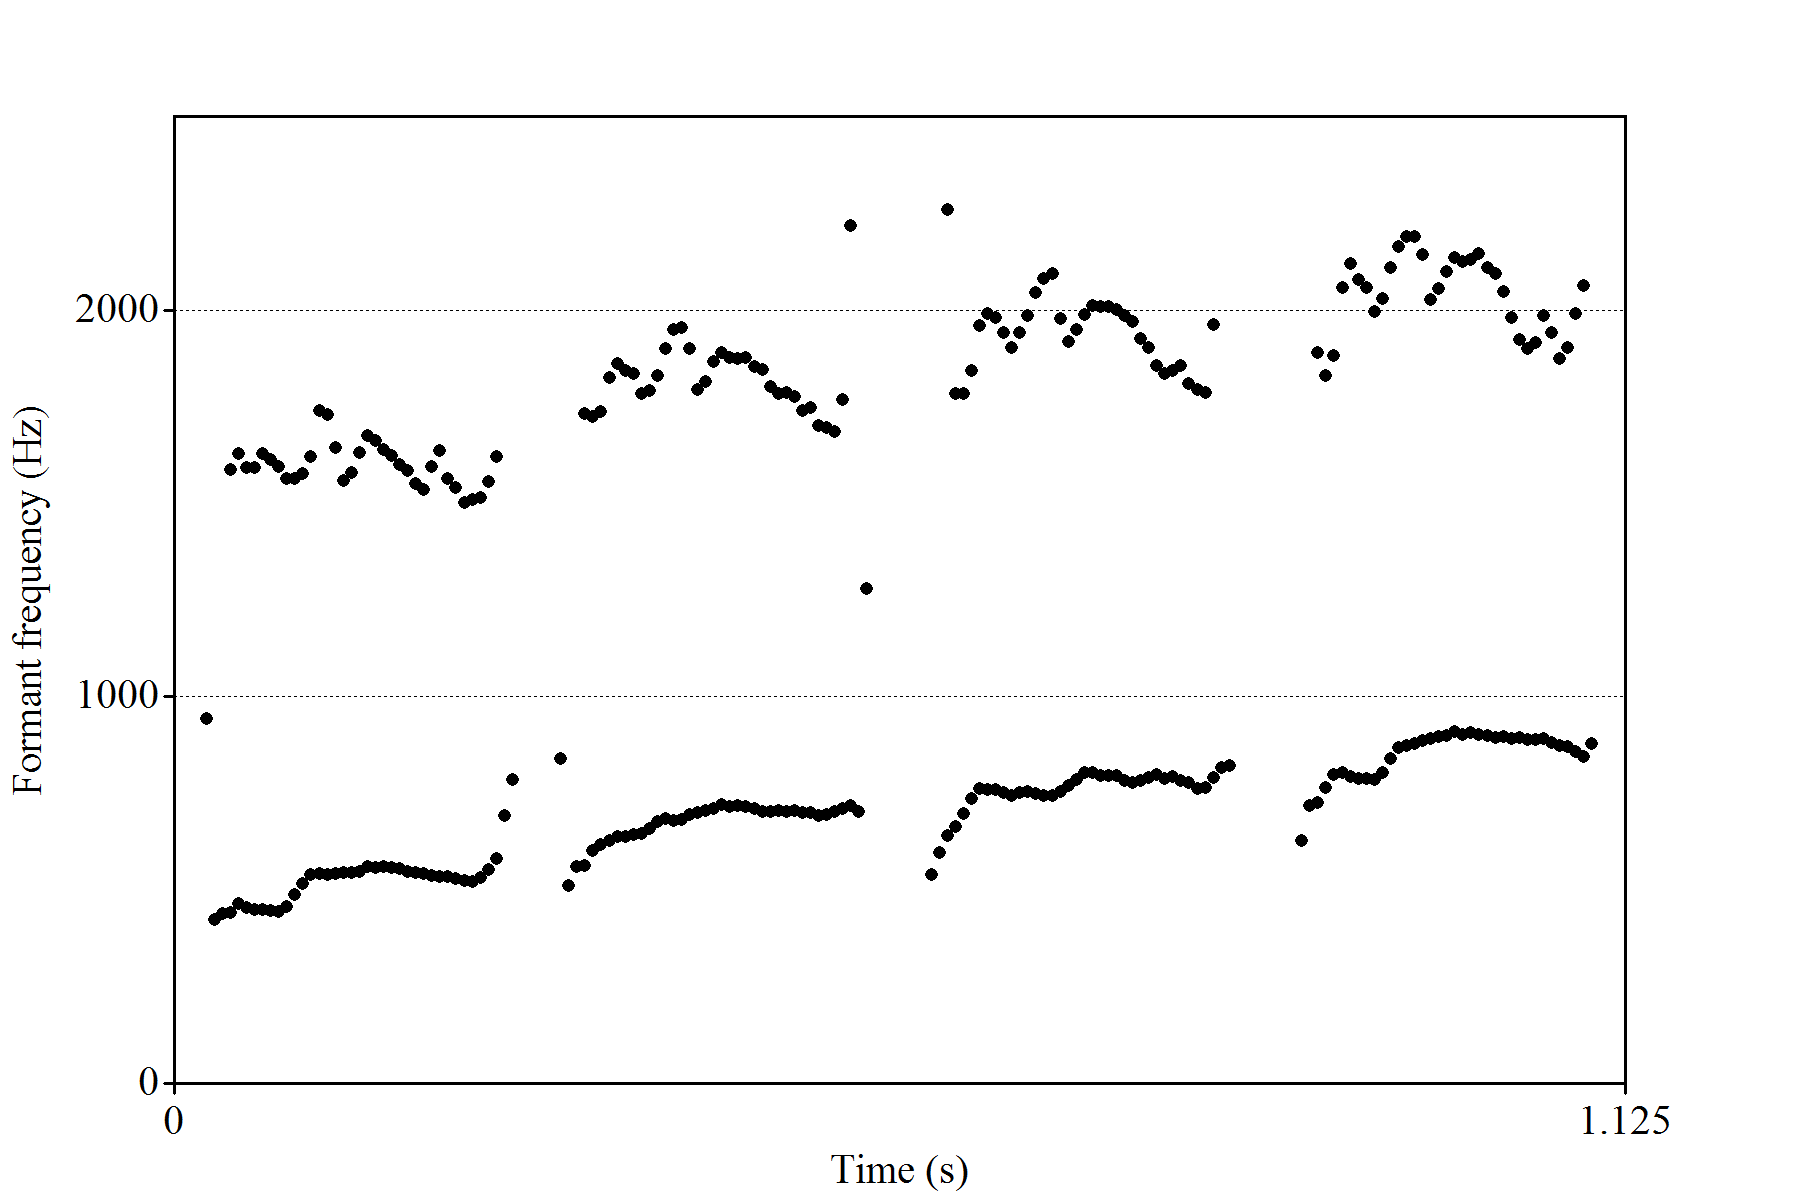
\includegraphics[width=0.75\textwidth]{./figures/fur_spectrogram.png}
	\caption{Formant tracks of \emph{fur} tokens}
	\label{fig.fur.spec}
\end{figure}

\tabref{tab.vowel.stimuli} summarises the final parameters, and \figref{fig.fur.spec} illustrates the result for one set of \textsc{nurse} tokens.
There was thus a continuum from stimulus 1 (hyper-Mancunian), to 2 (actual) and 3 (Scouse), to stimulus 4 (hyper-Scouse).
The formant structure of stimulus 2 was not modified, but still re-synthesis\is{resynthesis}ed so as not to stick out as the only completely natural recording.
For \textsc{nurse} stimulus 1 was thus higher and further back than the speaker's natural realisation, while stimuli 3 and 4 were both fronted and lowered to varying degrees.
With respect to happ\textsc{y}, stimulus 1 was lowered and centralised, while stimuli 3 and 4 were higher and fronter than the vowel that actually occurred in the recordings.
Participants always heard the re-synthesis\is{resynthesis}ed words in the same order (1 to 4).
Unfortunately, it was not possible to synthesis\is{resynthesis}e stimuli of satisfactory quality from the sentences that had happ\textsc{y} in phrase-final position (where it was typically realised as [ə], and often articulated with breathy voice).
For this reason, answer tokens for these sentences were taken from the equivalent recordings where happ\textsc{y} occurred in the middle of the sentence (and in the same carrier word).
Crucially, however, the realisation of happ\textsc{y} in the stimulus sentence itself was not altered.
With hindsight, this should have been avoided as this procedure created a confound with the independent variable `position of keyword in sentence' (cf. \sectref{sec.perc_res.happy}).

\subsection{Consonant stimuli}\label{sec.perc_method.con}

An equivalent procedure was developed for the consonants /ŋ(g)/ and /k/.
The link between those two in the context of this study is that the proportion of friction/aspiration is higher in the Scouse than in the standard British English variants, and this criterion was used to build a continuum similar to the one created for the two vowels.
Once more, the goal was to create roughly equal \isi{perceptual distance} (again checked auditorily by the author) between any two tokens, just as for the re-synthesis\is{resynthesis}ed vowels.
For every keyword a TextGrid was prepared which marked phases of aspiration, burst, and silence (for /k/) or nasality (for /ŋ(g)/) respectively (cf. \figref{fig.chicken.spec}).
For /ŋ(g)/, a script written by the author of this study then

\begin{enumerate}
	\item cut away the aspiration for stimulus 3,
	\item additionally cut away the burst for stimulus 2 (leaving only the nasal),
	\item and shortened the (often rather long) nasal by 25\% to arrive at a more standard-like length for stimulus 1.
\end{enumerate}

\begin{figure}
	
	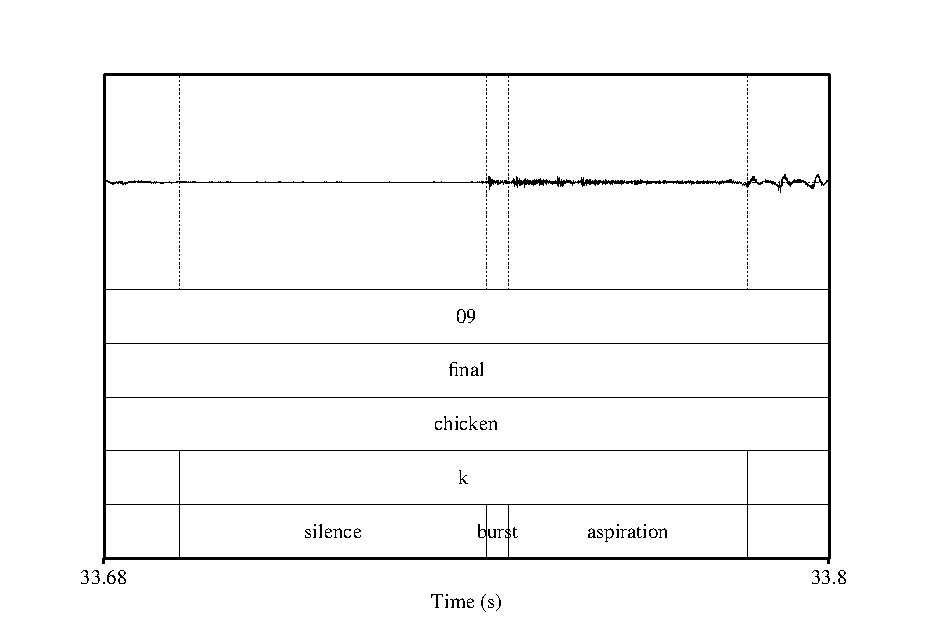
\includegraphics[width=0.75\textwidth]{./figures/chicken_spectrogram}
	\caption{Waveform and TextGrid for \emph{chicken} stimuli}
	\label{fig.chicken.spec}
\end{figure}

Stimulus 4 was the full, unaltered velar nasal plus realisation [ŋg].
To make the velar nasal plus sentences comparable to those of the other variables, stimulus 2 was afterwards copied back into the sentence to replace the natural [ŋg] realisation.
There was thus no voiced velar plosive present in the sentences subjects heard, and the continuum of stimuli was structured in the same way as those for the vowels and for /k/ in the sense that stimulus number 2 was the objectively most accurate choice that corresponded best to the sound actually used in the sentence.

Stimulus 2 for /k/ was the actual released plosive [k] as it occurred in the sentence recordings.
The hyper-Mancunian stimulus was created from this by cutting the aspiration, but leaving in the burst.
The speaker had also recorded all the /k/ sentences using the Scouse fricative variants.
The frication from these variants was pasted into the place of the original aspiration to form an affricate stimulus 3 (to make the result more natural sounding half of the closure phase was also deleted).
Stimulus 4, finally, had the whole plosive (silence, burst, and aspiration) replaced by the fricative by way of removing remaining silence and burst from stimulus 3.

For both /ŋ(g)/ and /k/, asymmetrical cross-fading and intensity adaptation was applied in intervocalic\is{phonological context} environments to create a smoother and less artificial transition from the nasal or the aspiration-less plosive to the following vowel in the hyper-Mancunian tokens (using a 25 milliseconds fade-in interval for the vowel and 50 milliseconds of overlap between phonemes when concatenating).
\tabref{tab.consonant.stimuli} provides an overview of the consonantal stimuli.

\begin{table}
	\caption{Structure of consonant stimuli}
	\label{tab.consonant.stimuli}
	
	\begin{tabular}{lll}
		\lsptoprule
		& /ŋg/ & /k/\\
		\midrule
		stimulus 1 & nasal only (shortened) & plosive with burst\\
		stimulus 2 & nasal only & plosive plus burst \& aspiration\\
		stimulus 3 & nasal plus burst & plosive plus burst \& frication\\
		stimulus 4 & nasal plus burst \& aspiration & fricative\\
		\lspbottomrule
	\end{tabular}
\end{table}

A small pilot study was run among linguists of the English Seminar at the University of Freiburg to make sure the stimuli (both the vocalic and the consonantal ones) were
\begin{inparaenum}[(a)]
	\item sufficiently natural-sounding, and
	\item equally distant from one another in perceptual terms.
\end{inparaenum}
This pilot study did not reveal any problems, so the investigation proper was carried out using these stimuli.

\section{Presentation}
\label{sec.perc_method.pres}

\subsection{Online platform}
\label{sec.perc_method.pres.platform}

The actual test was administered online using \textcite{sosci}, a professional tool for academic online surveys and questionnaires.
The platform uses flash to play audio and video files.
Although declining in importance, flash is still installed on most desktop and laptop computers (though not on tablets and smartphones) so the vast majority of potential subjects should have had no technical problems related to the website.
Nevertheless, participants first of all had to answer a filter question to make sure they had flash installed and activated and could actually play the sound recordings.
Subjects were given the hint that they were going to hear the name of a type of bird and the questionnaire then used the flash plug-in to play a short sound file of the speaker saying \emph{raven}.
Participants then typed in the word they had heard.
Wrong answers to this test question prevented the user from progressing in the questionnaire.
Participants were randomly assigned to one of two groups.
The control group was (correctly) told that the speaker they were going to listen to was from Manchester.
The other group was led to believe that the speaker was from Liverpool (about 1 in 3 of the participants who lived outside of Liverpool actually believed this).
Depending on which group subjects had been assigned to, `Manchester' or `Liverpool' was displayed at the top of every page as a reminder (cf. \figref{fig.online.screenshot}).

\begin{figure}
	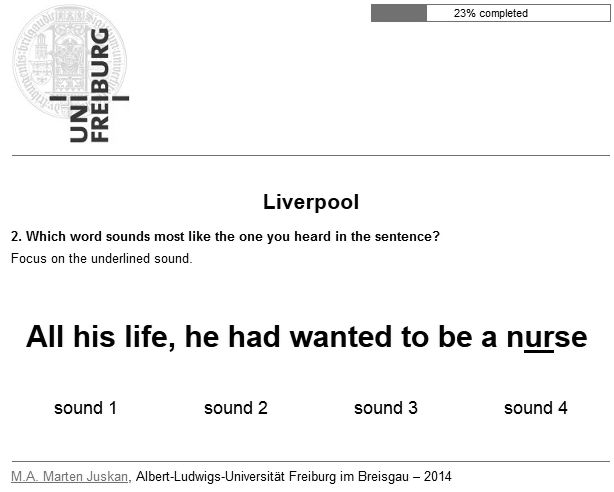
\includegraphics[width=\textwidth]{./figures/questionnaire_screenshot}
	\caption{Online questionnaire - training item}
	\label{fig.online.screenshot}
\end{figure}

After a couple of practice items (the results of which did not enter the analysis) participants were presented with 6 groups of 8 test tokens each.
Both the order of the groups and the order of the items within each group was randomised.
For every sentence, subjects were asked to pay special \isi{attention} to the (part of the) word that was underlined.
The sound files that were played had been created using another Praat script written by the author which pasted the stimulus sentence together with the resynthesis\is{resynthesis}ed keywords and added bits of silence in between (\figref{fig.per.sentence} visualises the structure).

\begin{figure}
	
	
	\begin{tikzpicture}[->,>=latex,shorten >= 5pt,shorten <= 5pt, ultra thick, align=center, node distance = 2cm, on grid, main node/.style={rectangle,draw}]
	\small
	
	\node (A) {silence\\1.5s};
	\node[right = of A] (B) {carrier\\ sentence};
	\node[right = of B] (C) {silence\\1.5s};
	\node[right = of C] (D) {`one'};
	\node[right = of D] (E) {silence\\0.5s};
	\node[right = of E] (F) {token\\1};
	\node[below = of F] (G) {silence\\1.5s};
	\node[left = of G] (H) {`two'};
	\node[left = of H] (I) {silence\\0.5s};
	\node[left = of I] (J) {token\\2};
	\node[left = of J] (K) {silence\\1.5s};															
	\node[left = of K] (L) {`three'};
	\node[below = of L] (M) {silence\\0.5s};
	\node[right = of M] (N) {token\\3};
	\node[right = of N] (O) {silence\\1.5s};
	\node[right = of O] (P) {`four'};
	\node[right = of P] (Q) {silence\\0.5s};
	\node[right = of Q] (R) {token\\4};
	
	\draw (A) -- (B);
	\draw (B) -- (C);
	\draw (C) -- (D);
	\draw (D) -- (E);								
	\draw (E) -- (F);
	\draw (F) -- (G);
	\draw (G) -- (H);
	\draw (H) -- (I);
	\draw (I) -- (J);
	\draw (J) -- (K);
	\draw (K) -- (L);
	\draw (L) -- (M);
	\draw (M) -- (N);
	\draw (N) -- (O);
	\draw (O) -- (P);
	\draw (P) -- (Q);
	\draw (Q) -- (R);
	
	\node[below = 1cm of {$(O)!0.5!(P)$}] (cutoff) {RT\\cut-off point};
	\node[above = 1cm of {$(O)!0.5!(P)$}] (help) {};
	
	\draw[-, dashed] (cutoff) edge (help);
	
	\end{tikzpicture}
	
	\caption{Timing of perception stimuli}
	\label{fig.per.sentence}
\end{figure}

\largerpage
Each sentence was presented on a separate page of the questionnaire.
Participants would see the sentence first for 1.5 seconds before the playback started automatically.
After the recording of the sentence had finished playing, participants heard the four resynthesis\is{resynthesis}ed words (introduced by ``one'', ``two'', ``three'', ```four'' to avoid confusion\footnote{The token numbers were recorded by a different female speaker (aged 26). This was not ideal as it is possible that the accent of the other speaker might have influenced participants. Incidentally, however, \citeauthor{haydrager2010} were faced with the same problem and correctly point out that any effect the second speaker \emph{might} have had would manifest itself in identical fashion in \emph{both} experimental conditions and should therefore not be able to confound the \isi{priming} effect \parencite[cf.][871 and 889]{haydrager2010}.}) with 1.5 seconds of silence in between words, and were asked to choose the one that they thought corresponded most closely to the sound in the test sentence.
Participants could either choose a sound by clicking on a button or by pressing ``1'', ``2'', ``3'', or ``4'' on their keyboard.
Both the sentence and the resynthesis\is{resynthesis}ed sounds were only played once.
As soon as the subject had clicked on the button of their choice (or pressed the relevant key) the next sentence was automatically presented.

\subsection{Reaction times}
\label{sec.perc_method.pres.rt}

Reaction times were also recorded.
These have to be taken with a grain of salt in the context of an online survey, as a number of external factors (skill in using a mouse etc.) add a lot of variance.
The potentially most important factor -- speed of internet connection -- can be ruled out as a confounding variable, however.
This is because the platform uses JavaScript to send each subset of stimuli to the computer of the subject.
Playback of the sound files does not start before all bits of the question have been downloaded.
RT measurements (with an accuracy of about 10 milliseconds) are then taken locally on the participant's computer before being bundled and sent back to the server.
No loading from the server takes place in between stimuli \parencite[cf.][]{sosci}.
While there is still some room for variation between different hardware configurations in terms of timing accuracy and the like, there is no reason to assume that one subgroup of participants in particular would be affected in a significantly different way, so overall such unwanted effects can be hoped to cancel out.
Furthermore, reaction times were not analysed as a dependent variable in its own right, but `merely' served to filter responses in the way described below.

The platform \citetitle{sosci} does come with some technical limitations, however, since it is not primarily designed for tests requiring RT measurements.
Unfortunately, it is neither possible to define a time window outside of which participants cannot enter a response nor to specify when the reaction time clock starts.
Technically speaking, RT measurements are really measurements of how long a subject spent on a particular page of the questionnaire.
Measuring thus starts automatically once the page is loaded and stops when the next page is accessed (which, in this study, happened automatically once an answer had been selected).
``Real'' reaction times are arrived at by substracting the total duration of each audio file from the time spent on the respective page.

As a consequence of these restrictions, it was possible for subjects to make their choice at any time, including \emph{before} the recording had actually finished even though the instructions spelled out that participants should listen to all answer options first.
It would have been quite easy to filter out all of these premature answers by simply eliminating all observations with negative RTs from the dataset.
This course of action was not taken for two reasons.
The first one is comparability with previous research.
Neither \citealt{niedzielski1999} nor \citealt{hayetal2006b,haydrager2010} even recorded reaction times and responses were given on a physical answer sheet so it is quite possible that these studies were, in part, based on answers that had been given before subjects had listened to all of their options.
The second, more important reason, is that it does not necessarily make sense to exclude an answer just because the subject did not listen to all resynthesis\is{resynthesis}ed sounds first.
After all, this study is interested in finding out how (stereotypical\is{stereotype}) expectations influence people's perception.
The claim that at least some expectations and \isi{attitude}s will prime\is{priming} people to perceive particular sounds \emph{implies} that at least to a certain extent the choice is already made before subjects can really process the physical signal and this might well show in negative RTs.
Many people might simply be reluctant to wait for the end of the recording if they already `know' the answer or if they have already heard the option that they think is the best match.
Ignoring negative RTs might then result in involuntarily eliminating (parts of) the \isi{priming} effect one is interested in from the dataset -- which might be a reason why previous studies have not even bothered with reaction times in the first place.

On the other hand, it is fortunate if one is able to cleanse the dataset of nonsense answers which are particularly likely to occur in an online test where the physical presence of the researcher cannot act as an incentive to take the task at hand seriously.
Responses with RTs that indicate the subject did not even listen to the carrier sentence, let alone the answer options, are clearly nothing but noise and should be eliminated from the sample.
As a sort of compromise it was decided to keep all responses that were not given more than 2000 milliseconds before the end of the stimulus.
This threshold ensures that the participant has listened to at least three of the four answer options (cf. \figref{fig.per.sentence}).
Responses that were given more than 4000 milliseconds after the end of the recording were likewise eliminated.

\section{Participants}\label{sec.perc_method.subjects}

Finding participants for the online test proved rather difficult.
Subjects were recruited through a number of channels.
A call for participants was distributed through Hope, Liverpool, and Manchester University.
Announcements posted in Liverpool and Manchester related groups on Facebook resulted in some (but very few) responses.
Some exchange students were recruited with the help of public notice boards on the campus of Freiburg University.
Several friends and colleagues were kind enough to spread the word via e-mail and social media, and this friend-of-a-friend approach proved to be comparatively fruitful.
Finally, personal contacts in Liverpool and Manchester and some of the people who had been interviewed about a year earlier were contacted and asked if they would like to participate.
All participants were required to\newpage 
\begin{enumerate}
	\item be British
	\item be native speakers of English
	\item have normal hearing
\end{enumerate}
The necessity of the last requirement should be obvious, as subjects were supposed to choose between audio stimuli that differed in rather subtle ways.
Requirements 1 and 2 were set to make sure participants were at least likely to have some degree of experience with or knowledge of the accents of Liverpool and Manchester.
After all, \isi{exemplar} \isi{priming} can only work if there are \isi{exemplar}s that can be activate\is{activation}d by the prime\is{priming}.
Given what \textcite{montgomery2007} found with respect to the status of Scouse in particular it seems not too far fetched to assume that people with British nationality (and native competence of English) have at least some \isi{exemplar}s indexed for `Liverpool', even if these are only derived from (stereotypical\is{stereotype}) media perform\is{accent performance}ances.
People from, say, the U.S. or Australia, on the other hand, will probably be a lot less familiar with the British accent landscape and might not have the slightest idea of what a Scouse accent sounds like -- either because they have never listened to someone from Liverpool, or because they have not done so \emph{knowingly}, meaning that the relevant \isi{exemplar}s will be indexed for a more general category such as `British'.
In both cases, \isi{priming} subjects for `Liverpool' (or `Manchester', for that matter) would not be possible.

At the end of the questionnaire, participants had to indicate their age, gender, educational level, profession (profession of parents for students), geographical origin and current town/city of residence (both via the first half of UK postcodes), and whether they self-identified as working or middle class.
The occupation scale was the simplified version of the National Statistics Socio-economic Classification, which is used, for instance, by the \citeauthor{nomis} and classifies jobs into lower, intermediate, and higher, primarily based on how much routine (at the lower end) and responsibility over others (at the upper end) is involved.
Just as for the interview data, levels of occupation and education were then used to classify subjects as belonging to one of the two broad categories `working class' or `middle class'.
Since this classification correlated strongly with the social class participants had explicitly chosen anyway, self-reported social class membership was used as a predictor for statistical modelling (see below).

On the basis of the postcodes participants provided, geographic coordinates were obtained from \url{http://xposition.co.uk/geopostcode/}, and a euclidean distance value was calculated for every subject using the following formula:
\begin{equation}
d = \sqrt{(lon_L - lon_s)^2 + (lat_L - lat_s)^2}
\end{equation}
Where \(lon_L\) and \(lat_L\) are the longitude and latitude of central L1 (Liverpool city centre), \(lon_s\) and \(lat_s\) the (central) coordinates of the subject's postcode, and \(d\) is the resulting distance value (the higher, the further the subject lives from Liverpool).
These figures are not, strictly speaking, directly comparable.
This is because 1 degree of longitude translates to a different absolute distance in kilometres or miles depending on the latitude.
Since the north-south extent of the UK is comparatively small, however, the amount of distortion introduced was considered negligible.
\figref{fig.per.subjects}\footnote{Map tiles by Stamen Design, under CC BY 3.0. Data by OpenStreetMap, under CC BY SA.} shows the geographical distribution of participants by representing every individual with a grey dot.
Two clusters are clearly visible, one in the north-west and one in the south-east of England.
The first is due to the fact that recruitment initially focussed on Liverpool and Manchester, while the London bias is to a degree even representative, given that between 15 and 20\% (depending on where one draws the boundaries) of the UK population live in the metropolitan area.
The remaining participants seem to come more or less from all over the country, although Wales and Northern Ireland are clearly under-represented.

\begin{figure}
	
	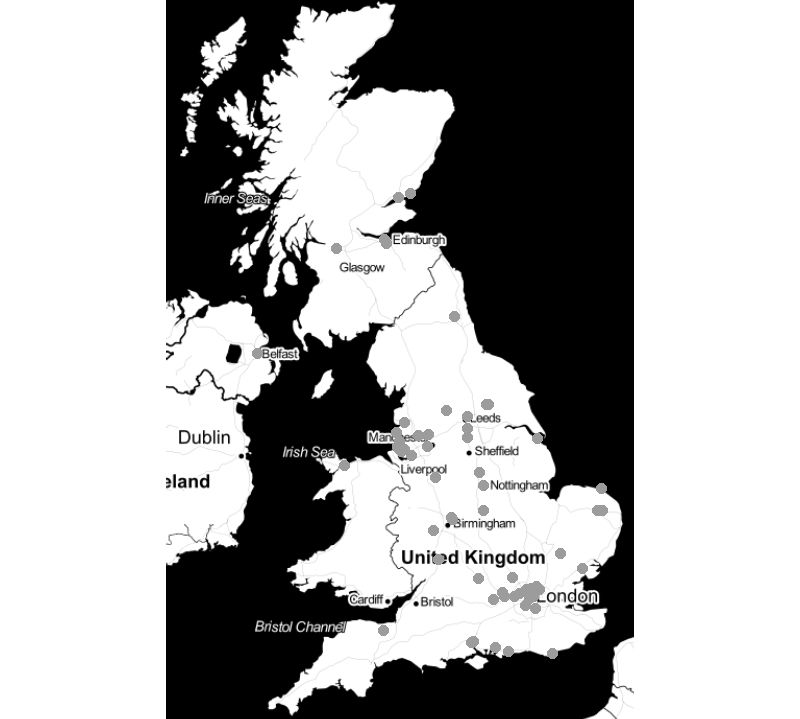
\includegraphics[width=0.49\textwidth]{./figures/participant_map}
	\caption{Geographical distribution of subjects (perception)}
	\label{fig.per.subjects}
\end{figure}

Subjects were given the opportunity to receive the results of the experiment after its completion and to participate in a lottery for a £100 gift card from a big online retailer.
E-mail-addresses were collected for these purposes, but kept strictly separate from the questionnaire responses (using an in-built function of the online platform specifically designed for that purpose).

\newpage 
In total, 67 subjects participated in the experiment and provided 2508 data points.
In addition to the more detailed placement via the postcode, participants were also assigned to one of the broad geographical categories ``internal'' (Liverpool and \isi{Merseyside}, ``L'' postcode area; 9 subjects) and ``external'' (everything else, 58 subjects).
It is possible that some of subjects in the Liverpool sample had already participated in one of the sociolinguistic interviews conducted by the author, but since these interviews had taken place (at least) a year earlier it is highly unlikely that this could have a distorting effect on results in the perception test.
\tabref{tab.participants.perception} provides a more detailed overview of the `external' sub-sample (3 subjects in this group declined to indicate their gender).
One thing that is immediately obvious is that the middle class is heavily over-represented, only 7 subjects were classified as belonging to the working class.
Among middle class subjects, female and male participants are not really evenly distributed across \isi{priming} conditions: women dominate in the group that was prime\is{priming}d for Liverpool, while men do in the other.
However, Prime and Gender are still not collinear in the dataset (κ= 1.54), and mixed-effects ordinal models regressing reported percept on Gender did not find a significant effect of the latter, neither in the `Liverpool' (p = 0.801) nor in the `Manchester' condition (p = 0.597).
In other words, women and men did not behave differently in this experiment so the fact that they are unevenly distributed across conditions is unproblematic.
Incidentally, \textcite[69 and 79--80]{niedzielski1999} also found that \enquote{there was essentially no difference between what male and female respondents selected}.

\begin{table}
	\caption[Gender and {social class} of subjects (perception)]{Gender and {social class} distribution of subjects (perception, external)}
	\label{tab.participants.perception}
	
	\begin{tabular}{lcccc}
		\lsptoprule
		prime\is{priming} & \multicolumn{2}{c}{`Liverpool'} & \multicolumn{2}{c}{`Manchester'}\\
		& F & M & F & M\\
		\midrule
		working class & 2 & 3 & 1 & 1\\
		middle class & 17 & 6 & 9 & 16\\
		\lspbottomrule
	\end{tabular}
\end{table}

\section{Statistical analysis}\label{sec.perc_method.stats}

Unlike in the case of the interview data where there were fewer participants and the role of the individual subject was different (cf. \sectref{sec.prod_method.stats}), it actually does make sense to include random effects for the statistical analysis of the perception data.

However, the data collected by the experiment described above are not ratio or interval scaled.
While answers are expressed in numbers (token 1, 2, 3, or 4), these are really labels for 4 distinct\is{distinctness} categories rather than measurements on a continuous scale.
There is no guarantee, for instance, that the (perceptual) distance from token 1 to token 2 is identical to that between tokens 2 and 3 (although this \emph{was} the aim when creating the tokens; cf.  \sectref{sec.perc_method.vow} and \sectref{sec.perc_method.con}) -- which is what the values suggest when they are being treated as numerical measurements.
On the other hand, the data \emph{are} ordered in a way (from most standard/Mancunian to most Liverpool), so while choosing token 4 instead of token 3 might not be the same as choosing 3 instead of 2 in terms of \isi{perceptual distance}, higher values do in all cases represent a more Liverpool-like percept than lower values -- much in the same way that, say, a higher RT always mean that a subject took more time to respond than another one with a lower RT.
It was therefore decided not to follow \citealt{hayetal2006a,haydrager2010} in treating the answers as numerical data for the purposes of statistical modelling.
Instead, the R package `ordinal' \parencite{Rordinal} was used to calculate cumulative link mixed ordered regression models via the Laplace approximation.

Subject was entered as a random intercept (cf. \sectref{sec.prod_method.stats}), and a random by-subject slope for stimulus order was also included to counter any individual training or fatigue effects.
Carrier word was not included as a random effect because \isi{frequency} and, for consonants, phonological environment\is{phonological context} were of interest as fixed effects.
Since there were only 6 keywords per variable filtering out any lexical effects would almost certainly also have eliminated effects of \isi{frequency} and/or phonological environment\is{phonological context}.
Prime was entered as a fixed factor, along with gender, social class (self-reported), age of the subject, and \isi{geographical distance} from Liverpool.
Furthermore, the Zipf\is{Zipf score} score of the carrier word was included, as was the position of the carrier word in the stimulus sentence (sentence-medially or -finally), the position of the stimulus sentence within the experiment (when was the sentence played to the subject), and, for consonants, the phonological environment\is{phonological context} (V\_V or \_\#).
All two-way interactions of the prime\is{priming} with these linguistic and extra-linguistic factors were also considered.
Sum coding was used for all models in order to be able to identify main effects and interactions.
Model selection was based on AIC scores and F-tests comparing nested models.
Collinearity\is{collinearity} was investigated applying the functions written by Austin Frank (cf. \sectref{sec.prod_method.stats}) to corresponding mixed-effects logistic regression models. %check indexing
\chapter{Perception results}
\label{ch.perc_res}

Originally, the intention of this study was to focus on the perception of Scouse variants by listeners from Liverpool and Manchester (in order to have a rough equivalent of the oppositions Michigan-Ontario in \citealt{niedzielski1999}, and Australia-New Zealand in \citealt{hayetal2006a}).
However, I only managed to recruit 9 subjects from the Liverpool/\isi{Merseyside} area and 3 from Greater Manchester over the course of the 15 months that the perception test was online, despite my own best efforts and notwithstanding the fact that many people with personal contacts in Liverpool and Manchester helped to spread the word.
A detailed analysis of such a small sample does not seem to make much sense.
All the same, the most basic tests were carried out on the Liverpool sub-sample as well, and, crucially, almost all results are comparable to those in the rest of the sample.
Mixed-effects ordinal models regressing reported percept on Area (\enquote*{internal} vs. \enquote*{external}) showed that the responses given by subjects from outside were not significantly different from those provided by participants from Liverpool as far as happ\textsc{y} (estimate = 0.025, se = 0.115, z value = 0.216, p = 0.829), \textsc{nurse} (estimate = -0.001, se = 0.185, z value = -0.007, p = 0.994), and /k/ (estimate = 0.053, se = 0.193, z value = 0.275, p = 0.783) are concerned.
This is also obvious when the relevant bar plots (not reported here) are compared with the ones generated on the basis of the `external' sample.
Furthermore, whenever there is a significant \isi{priming} effect in the Liverpool sub-sample, this effect is in the same (unexpected) direction as the ones reported below for perceivers from outside of the city.

For velar nasal plus, on the other hand, there is a statistical trend (estimate = -0.382, se = 0.210, z value = -1.815, p = 0.070).
With respect to this variable, the difference between \isi{priming} conditions is more pronounced for subjects from Liverpool, and the effect is in the opposite direction compared to the remaining participants from the rest of the country.
The production data suggest that velar nasal plus carries at least some social meaning, but this result \emph{could} indicate that it is actually even more salient\is{salience} in Liverpool than suspected, despite the fact that nobody comments on it.
This variable could present a fruitful area of future research, but it should be borne in mind that these statements are based on a very small and unbalanced sample, which means that we might well be talking about a non-issue because the effect would disappear in a larger dataset.

In any case, /ŋ(g)/ is the only variable where results seem to diverge.
With respect to the other three, perceivers from Liverpool and elsewhere do not exhibit any statistically meaningful differences in behaviour.
In addition, it has been shown that impersonations and comments by outsiders have an impact on what variables Liverpudlians themselves are conscious\is{awareness}ly aware\is{awareness} of (cf. Chapter \ref{prod.res.qual}), so internal and external \isi{salience} correlate to a degree and are not completely unrelated.
For these reason I would argue that it does not appear completely unjustified to assume that most of what is described below would also hold in a larger sample of listeners from Liverpool, but this claim is in need of proper empirical confirmation in the future.
All further results reported in this chapter are exclusively based on responses provided by people living outside of Liverpool.

\section{happ\textsc{y}}
\label{sec.perc_res.happy}
	\subsection{Overview}
	\label{sec.perc_res.happy.overview}

As described in Section \ref{sec.perc_method.stats}, a mixed-effects ordinal regression model was fit to the data by hand.
This maximal model did not contain any troubling \isi{collinearity} (κ = 13.99), but for reasons of comparability (cf. \ref{sec.perc_res.nurse}, \ref{sec.perc_res.ng}, and \ref{sec.perc_res.k}), the \isi{frequency} of the keyword expressed in Zipf\is{Zipf score} scores, as well as the interaction of Zipf\is{Zipf score} score and \isi{priming} condition, were removed from the model.\footnote{When Zipf\is{Zipf score} scores are included they show up as a significant predictor in the corresponding minimal adequate model (p < 0.001). The same is true for position of keyword (p < 0.001) and age of participant (p = 0.043). In addition, \isi{geographical distance} from Liverpool almost reaches statistical significance as well (p = 0.080). Frequency\is{frequency} and age are therefore briefly discussed below for the sake of completeness.}
Collinearity\is{collinearity} was further reduced this way (κ = 10.61).
Model selection based on AIC scores and F-tests comparing nested models resulted in the minimal adequate model printed below.
Only two factors show up as main effects (one of them not quite significant) and no statistically significant interactions could be found.
Position of the stimulus (in the middle or at the end of the sentence) is a highly significant predictor.
Geographical distance of the participant from Liverpool does not reach significance at the 5\% level, but the p-value is low enough to qualify as a statistical trend.
For this reason the factor was kept in the model.

\begin{table}[h]
	\caption{happ\textsc{y} (perception): mixed-effects ordinal regression}
	\centering
	\begin{tabular}{p{0.3\textwidth}rrrrl}
		\hline
		Fixed effects: & Estimate & Std. Error &  z value & Pr($>$$|$z$|$) & \\ 
		\hline
		POSfinal & -0.932 & 0.091 & -10.194 & <0.001 & ***\\ 
		DISTANCE & 0.169 & 0.093 & 1.811 & 0.070 & .\\ 
		\hline
		Random effects: & & & & & \\
		Groups &         Name & Variance &      Std.Dev. & & \\
		QUESTIONNAIRE &  (Intercept) & 0.162 & 0.402 & & \\
		QUESTIONNAIRE & TOKEN      & <0.001 & <0.001 & & \\
		\multicolumn{3}{l}{(number of obs: 516, groups: QUESTIONNAIRE, 55)} & & & \\
		\hline
	\end{tabular}
\end{table}

\subsection{Prime}
\label{sec.perc_res.happy.prime}

Prime is not among the fixed effects.
This indicates that for the happ\textsc{y} stimuli it did not make a difference whether participants thought they were listening to a speaker from Liverpool or Manchester.
Figure \ref{fig.bar.happy.tot.ext} visualises this fact.
As with all the following bar plots in this chapter, answers from subjects who were prime\is{priming}d for ``Liverpool'' are represented by black bars, those given by people who were correctly told the speaker was from Manchester are visualised by light grey bars.

\begin{figure}[h]
	\centering
		\definecolor{shadecolor}{rgb}{0.969, 0.969, 0.969}
		\resizebox{.49\linewidth}{!}{% Created by tikzDevice version 0.10.1 on 2017-04-14 13:58:29
% !TEX encoding = UTF-8 Unicode
\begin{tikzpicture}[x=1pt,y=1pt]
\definecolor{fillColor}{RGB}{255,255,255}
\path[use as bounding box,fill=fillColor,fill opacity=0.00] (0,0) rectangle (505.89,505.89);
\begin{scope}
\path[clip] (  0.00,  0.00) rectangle (505.89,505.89);
\definecolor{drawColor}{RGB}{255,255,255}
\definecolor{fillColor}{RGB}{255,255,255}

\path[draw=drawColor,line width= 0.6pt,line join=round,line cap=round,fill=fillColor] (  0.00,  0.00) rectangle (505.89,505.89);
\end{scope}
\begin{scope}
\path[clip] ( 64.22, 62.51) rectangle (500.39,462.54);
\definecolor{fillColor}{RGB}{255,255,255}

\path[fill=fillColor] ( 64.22, 62.51) rectangle (500.39,462.54);
\definecolor{drawColor}{gray}{0.92}

\path[draw=drawColor,line width= 0.3pt,line join=round] ( 64.22,126.16) --
	(500.39,126.16);

\path[draw=drawColor,line width= 0.3pt,line join=round] ( 64.22,217.07) --
	(500.39,217.07);

\path[draw=drawColor,line width= 0.3pt,line join=round] ( 64.22,307.99) --
	(500.39,307.99);

\path[draw=drawColor,line width= 0.3pt,line join=round] ( 64.22,398.90) --
	(500.39,398.90);

\path[draw=drawColor,line width= 0.6pt,line join=round] ( 64.22, 80.70) --
	(500.39, 80.70);

\path[draw=drawColor,line width= 0.6pt,line join=round] ( 64.22,171.61) --
	(500.39,171.61);

\path[draw=drawColor,line width= 0.6pt,line join=round] ( 64.22,262.53) --
	(500.39,262.53);

\path[draw=drawColor,line width= 0.6pt,line join=round] ( 64.22,353.44) --
	(500.39,353.44);

\path[draw=drawColor,line width= 0.6pt,line join=round] ( 64.22,444.36) --
	(500.39,444.36);

\path[draw=drawColor,line width= 0.6pt,line join=round] (126.53, 62.51) --
	(126.53,462.54);

\path[draw=drawColor,line width= 0.6pt,line join=round] (230.38, 62.51) --
	(230.38,462.54);

\path[draw=drawColor,line width= 0.6pt,line join=round] (334.23, 62.51) --
	(334.23,462.54);

\path[draw=drawColor,line width= 0.6pt,line join=round] (438.08, 62.51) --
	(438.08,462.54);
\definecolor{fillColor}{gray}{0.80}

\path[fill=fillColor] (126.53, 80.70) rectangle (173.26,179.13);
\definecolor{fillColor}{gray}{0.20}

\path[fill=fillColor] ( 79.80, 80.70) rectangle (126.53,183.18);
\definecolor{fillColor}{gray}{0.80}

\path[fill=fillColor] (230.38, 80.70) rectangle (277.11,231.03);
\definecolor{fillColor}{gray}{0.20}

\path[fill=fillColor] (183.65, 80.70) rectangle (230.38,242.69);
\definecolor{fillColor}{gray}{0.80}

\path[fill=fillColor] (334.23, 80.70) rectangle (380.96,214.92);
\definecolor{fillColor}{gray}{0.20}

\path[fill=fillColor] (287.50, 80.70) rectangle (334.23,209.63);
\definecolor{fillColor}{gray}{0.80}

\path[fill=fillColor] (438.08, 80.70) rectangle (484.81,152.28);
\definecolor{fillColor}{gray}{0.20}

\path[fill=fillColor] (391.35, 80.70) rectangle (438.08,141.86);
\definecolor{drawColor}{gray}{0.20}

\path[draw=drawColor,line width= 0.6pt,line join=round,line cap=round] ( 64.22, 62.51) rectangle (500.39,462.54);
\end{scope}
\begin{scope}
\path[clip] (  0.00,  0.00) rectangle (505.89,505.89);
\definecolor{drawColor}{gray}{0.30}

\node[text=drawColor,anchor=base east,inner sep=0pt, outer sep=0pt, scale=  1.60] at ( 59.27, 74.66) {0{\%}};

\node[text=drawColor,anchor=base east,inner sep=0pt, outer sep=0pt, scale=  1.60] at ( 59.27,165.58) {20{\%}};

\node[text=drawColor,anchor=base east,inner sep=0pt, outer sep=0pt, scale=  1.60] at ( 59.27,256.49) {40{\%}};

\node[text=drawColor,anchor=base east,inner sep=0pt, outer sep=0pt, scale=  1.60] at ( 59.27,347.41) {60{\%}};

\node[text=drawColor,anchor=base east,inner sep=0pt, outer sep=0pt, scale=  1.60] at ( 59.27,438.32) {80{\%}};
\end{scope}
\begin{scope}
\path[clip] (  0.00,  0.00) rectangle (505.89,505.89);
\definecolor{drawColor}{gray}{0.20}

\path[draw=drawColor,line width= 0.6pt,line join=round] ( 61.47, 80.70) --
	( 64.22, 80.70);

\path[draw=drawColor,line width= 0.6pt,line join=round] ( 61.47,171.61) --
	( 64.22,171.61);

\path[draw=drawColor,line width= 0.6pt,line join=round] ( 61.47,262.53) --
	( 64.22,262.53);

\path[draw=drawColor,line width= 0.6pt,line join=round] ( 61.47,353.44) --
	( 64.22,353.44);

\path[draw=drawColor,line width= 0.6pt,line join=round] ( 61.47,444.36) --
	( 64.22,444.36);
\end{scope}
\begin{scope}
\path[clip] (  0.00,  0.00) rectangle (505.89,505.89);
\definecolor{drawColor}{gray}{0.20}

\path[draw=drawColor,line width= 0.6pt,line join=round] (126.53, 59.76) --
	(126.53, 62.51);

\path[draw=drawColor,line width= 0.6pt,line join=round] (230.38, 59.76) --
	(230.38, 62.51);

\path[draw=drawColor,line width= 0.6pt,line join=round] (334.23, 59.76) --
	(334.23, 62.51);

\path[draw=drawColor,line width= 0.6pt,line join=round] (438.08, 59.76) --
	(438.08, 62.51);
\end{scope}
\begin{scope}
\path[clip] (  0.00,  0.00) rectangle (505.89,505.89);
\definecolor{drawColor}{gray}{0.30}

\node[text=drawColor,anchor=base,inner sep=0pt, outer sep=0pt, scale=  1.60] at (126.53, 45.50) {1 [ə]};

\node[text=drawColor,anchor=base,inner sep=0pt, outer sep=0pt, scale=  1.60] at (126.53, 28.22) { ←more Manchester};

\node[text=drawColor,anchor=base,inner sep=0pt, outer sep=0pt, scale=  1.60] at (230.38, 45.50) {2 [ɪ]};

\node[text=drawColor,anchor=base,inner sep=0pt, outer sep=0pt, scale=  1.60] at (334.23, 45.50) {3 [ï]};

\node[text=drawColor,anchor=base,inner sep=0pt, outer sep=0pt, scale=  1.60] at (438.08, 45.50) {4 [i]};

\node[text=drawColor,anchor=base,inner sep=0pt, outer sep=0pt, scale=  1.60] at (438.08, 28.22) { more Liverpool→};
\end{scope}
\begin{scope}
\path[clip] (  0.00,  0.00) rectangle (505.89,505.89);
\definecolor{drawColor}{RGB}{0,0,0}

\node[text=drawColor,anchor=base,inner sep=0pt, outer sep=0pt, scale=  2.00] at (282.31,  7.63) {reported percept};
\end{scope}
\begin{scope}
\path[clip] (  0.00,  0.00) rectangle (505.89,505.89);
\definecolor{drawColor}{RGB}{0,0,0}

\node[text=drawColor,rotate= 90.00,anchor=base,inner sep=0pt, outer sep=0pt, scale=  2.00] at ( 20.59,262.53) {of cases};
\end{scope}
\begin{scope}
\path[clip] (  0.00,  0.00) rectangle (505.89,505.89);
\definecolor{fillColor}{RGB}{255,255,255}

\path[fill=fillColor] (130.20,473.92) rectangle (434.41,500.39);
\end{scope}
\begin{scope}
\path[clip] (  0.00,  0.00) rectangle (505.89,505.89);
\definecolor{drawColor}{RGB}{0,0,0}

\node[text=drawColor,anchor=base west,inner sep=0pt, outer sep=0pt, scale=  2.00] at (135.89,479.61) {prime};
\end{scope}
\begin{scope}
\path[clip] (  0.00,  0.00) rectangle (505.89,505.89);
\definecolor{fillColor}{RGB}{255,255,255}

\path[fill=fillColor] (194.31,479.61) rectangle (208.77,494.70);
\end{scope}
\begin{scope}
\path[clip] (  0.00,  0.00) rectangle (505.89,505.89);
\definecolor{fillColor}{gray}{0.20}

\path[fill=fillColor] (195.02,480.32) rectangle (208.05,493.99);
\end{scope}
\begin{scope}
\path[clip] (  0.00,  0.00) rectangle (505.89,505.89);
\definecolor{fillColor}{RGB}{255,255,255}

\path[fill=fillColor] (302.78,479.61) rectangle (317.23,494.70);
\end{scope}
\begin{scope}
\path[clip] (  0.00,  0.00) rectangle (505.89,505.89);
\definecolor{fillColor}{gray}{0.80}

\path[fill=fillColor] (303.49,480.32) rectangle (316.52,493.99);
\end{scope}
\begin{scope}
\path[clip] (  0.00,  0.00) rectangle (505.89,505.89);
\definecolor{drawColor}{RGB}{0,0,0}

\node[text=drawColor,anchor=base west,inner sep=0pt, outer sep=0pt, scale=  2.00] at (210.57,479.61) {Liverpool};
\end{scope}
\begin{scope}
\path[clip] (  0.00,  0.00) rectangle (505.89,505.89);
\definecolor{drawColor}{RGB}{0,0,0}

\node[text=drawColor,anchor=base west,inner sep=0pt, outer sep=0pt, scale=  2.00] at (319.04,479.61) {Manchester};
\end{scope}
\end{tikzpicture}
} 
	\caption{happ\textsc{y} (perception) by prime}
	\label{fig.bar.happy.tot.ext}
\end{figure}

There is a slight preference for stimulus number 2 (the one actually present in the stimulus sentences) at around 35\% of answers given, followed by the somewhat tenser (and more Liverpool-like) stimulus 3 at just below 30\%.
The `hyper-Mancunian' and `hyper-Liverpool' stimuli 1 (about 20\%) and 4 (15--17\%) were less frequently chosen.
The crucial point, however, is that only marginal differences between the two conditions are visible, which corroborates the result of the mixed-effects model that subjects were not influenced by the prime\is{priming} when perceiving happ\textsc{y}-stimuli.

\subsection{Position of carrier word}
\label{sec.perc_res.happy.position}

Figure \ref{fig.bar.happy.tot.ext.pos} shows the clear influence of carrier word position within the stimulus sentence that was identified as a significant predictor by the mixed-effects model.
Perception of sentence-final stimuli can be said to be more objective as participants chose stimulus 2 (which actually occurred in the recording) in around 45\% of cases.
The hyper-centralised stimulus 1 was, at about 35\%, also quite frequent, whereas the `Liverpool' stimuli 3 and 4 only account for 20\% of answers, with stimulus 4 being particularly rare.
When the carrier word was presented in the middle of the sentence, subjects most often reported having heard stimulus number 3, a vowel higher and fronter than in the actual recording.
Stimuli 2 and 4 were both chosen around 25--30\% of the time, while the hyper-Mancunian vowel was only selected in a bit more than 10\% of cases.
Overall then, participants were more likely to perceive a `Liverpool'-type tenser /i/ when the carrier word was presented in the middle of the sentence than when it occurred as the last word in the sentence.

\begin{figure}[h]
	\centering
	\begin{subfigure}{0.49\textwidth}
		\centering
			\definecolor{shadecolor}{rgb}{0.969, 0.969, 0.969}
			\resizebox{\linewidth}{!}{% Created by tikzDevice version 0.10.1 on 2017-04-14 14:06:46
% !TEX encoding = UTF-8 Unicode
\begin{tikzpicture}[x=1pt,y=1pt]
\definecolor{fillColor}{RGB}{255,255,255}
\path[use as bounding box,fill=fillColor,fill opacity=0.00] (0,0) rectangle (505.89,505.89);
\begin{scope}
\path[clip] (  0.00,  0.00) rectangle (505.89,505.89);
\definecolor{drawColor}{RGB}{255,255,255}
\definecolor{fillColor}{RGB}{255,255,255}

\path[draw=drawColor,line width= 0.6pt,line join=round,line cap=round,fill=fillColor] (  0.00,  0.00) rectangle (505.89,505.89);
\end{scope}
\begin{scope}
\path[clip] ( 64.22, 62.51) rectangle (500.39,462.54);
\definecolor{fillColor}{RGB}{255,255,255}

\path[fill=fillColor] ( 64.22, 62.51) rectangle (500.39,462.54);
\definecolor{drawColor}{gray}{0.92}

\path[draw=drawColor,line width= 0.3pt,line join=round] ( 64.22,126.16) --
	(500.39,126.16);

\path[draw=drawColor,line width= 0.3pt,line join=round] ( 64.22,217.07) --
	(500.39,217.07);

\path[draw=drawColor,line width= 0.3pt,line join=round] ( 64.22,307.99) --
	(500.39,307.99);

\path[draw=drawColor,line width= 0.3pt,line join=round] ( 64.22,398.90) --
	(500.39,398.90);

\path[draw=drawColor,line width= 0.6pt,line join=round] ( 64.22, 80.70) --
	(500.39, 80.70);

\path[draw=drawColor,line width= 0.6pt,line join=round] ( 64.22,171.61) --
	(500.39,171.61);

\path[draw=drawColor,line width= 0.6pt,line join=round] ( 64.22,262.53) --
	(500.39,262.53);

\path[draw=drawColor,line width= 0.6pt,line join=round] ( 64.22,353.44) --
	(500.39,353.44);

\path[draw=drawColor,line width= 0.6pt,line join=round] ( 64.22,444.36) --
	(500.39,444.36);

\path[draw=drawColor,line width= 0.6pt,line join=round] (126.53, 62.51) --
	(126.53,462.54);

\path[draw=drawColor,line width= 0.6pt,line join=round] (230.38, 62.51) --
	(230.38,462.54);

\path[draw=drawColor,line width= 0.6pt,line join=round] (334.23, 62.51) --
	(334.23,462.54);

\path[draw=drawColor,line width= 0.6pt,line join=round] (438.08, 62.51) --
	(438.08,462.54);
\definecolor{fillColor}{gray}{0.80}

\path[fill=fillColor] (126.53, 80.70) rectangle (173.26,122.98);
\definecolor{fillColor}{gray}{0.20}

\path[fill=fillColor] ( 79.80, 80.70) rectangle (126.53,133.63);
\definecolor{fillColor}{gray}{0.80}

\path[fill=fillColor] (230.38, 80.70) rectangle (277.11,189.94);
\definecolor{fillColor}{gray}{0.20}

\path[fill=fillColor] (183.65, 80.70) rectangle (230.38,205.24);
\definecolor{fillColor}{gray}{0.80}

\path[fill=fillColor] (334.23, 80.70) rectangle (380.96,253.37);
\definecolor{fillColor}{gray}{0.20}

\path[fill=fillColor] (287.50, 80.70) rectangle (334.23,248.83);
\definecolor{fillColor}{gray}{0.80}

\path[fill=fillColor] (438.08, 80.70) rectangle (484.81,211.08);
\definecolor{fillColor}{gray}{0.20}

\path[fill=fillColor] (391.35, 80.70) rectangle (438.08,189.67);
\definecolor{drawColor}{gray}{0.20}

\path[draw=drawColor,line width= 0.6pt,line join=round,line cap=round] ( 64.22, 62.51) rectangle (500.39,462.54);
\end{scope}
\begin{scope}
\path[clip] (  0.00,  0.00) rectangle (505.89,505.89);
\definecolor{drawColor}{gray}{0.30}

\node[text=drawColor,anchor=base east,inner sep=0pt, outer sep=0pt, scale=  1.60] at ( 59.27, 74.66) {0{\%}};

\node[text=drawColor,anchor=base east,inner sep=0pt, outer sep=0pt, scale=  1.60] at ( 59.27,165.58) {20{\%}};

\node[text=drawColor,anchor=base east,inner sep=0pt, outer sep=0pt, scale=  1.60] at ( 59.27,256.49) {40{\%}};

\node[text=drawColor,anchor=base east,inner sep=0pt, outer sep=0pt, scale=  1.60] at ( 59.27,347.41) {60{\%}};

\node[text=drawColor,anchor=base east,inner sep=0pt, outer sep=0pt, scale=  1.60] at ( 59.27,438.32) {80{\%}};
\end{scope}
\begin{scope}
\path[clip] (  0.00,  0.00) rectangle (505.89,505.89);
\definecolor{drawColor}{gray}{0.20}

\path[draw=drawColor,line width= 0.6pt,line join=round] ( 61.47, 80.70) --
	( 64.22, 80.70);

\path[draw=drawColor,line width= 0.6pt,line join=round] ( 61.47,171.61) --
	( 64.22,171.61);

\path[draw=drawColor,line width= 0.6pt,line join=round] ( 61.47,262.53) --
	( 64.22,262.53);

\path[draw=drawColor,line width= 0.6pt,line join=round] ( 61.47,353.44) --
	( 64.22,353.44);

\path[draw=drawColor,line width= 0.6pt,line join=round] ( 61.47,444.36) --
	( 64.22,444.36);
\end{scope}
\begin{scope}
\path[clip] (  0.00,  0.00) rectangle (505.89,505.89);
\definecolor{drawColor}{gray}{0.20}

\path[draw=drawColor,line width= 0.6pt,line join=round] (126.53, 59.76) --
	(126.53, 62.51);

\path[draw=drawColor,line width= 0.6pt,line join=round] (230.38, 59.76) --
	(230.38, 62.51);

\path[draw=drawColor,line width= 0.6pt,line join=round] (334.23, 59.76) --
	(334.23, 62.51);

\path[draw=drawColor,line width= 0.6pt,line join=round] (438.08, 59.76) --
	(438.08, 62.51);
\end{scope}
\begin{scope}
\path[clip] (  0.00,  0.00) rectangle (505.89,505.89);
\definecolor{drawColor}{gray}{0.30}

\node[text=drawColor,anchor=base,inner sep=0pt, outer sep=0pt, scale=  1.60] at (126.53, 45.50) {1 [ə]};

\node[text=drawColor,anchor=base,inner sep=0pt, outer sep=0pt, scale=  1.60] at (126.53, 28.22) { ←more Manchester};

\node[text=drawColor,anchor=base,inner sep=0pt, outer sep=0pt, scale=  1.60] at (230.38, 45.50) {2 [ɪ]};

\node[text=drawColor,anchor=base,inner sep=0pt, outer sep=0pt, scale=  1.60] at (334.23, 45.50) {3 [ï]};

\node[text=drawColor,anchor=base,inner sep=0pt, outer sep=0pt, scale=  1.60] at (438.08, 45.50) {4 [i]};

\node[text=drawColor,anchor=base,inner sep=0pt, outer sep=0pt, scale=  1.60] at (438.08, 28.22) { more Liverpool→};
\end{scope}
\begin{scope}
\path[clip] (  0.00,  0.00) rectangle (505.89,505.89);
\definecolor{drawColor}{RGB}{0,0,0}

\node[text=drawColor,anchor=base,inner sep=0pt, outer sep=0pt, scale=  2.00] at (282.31,  7.63) {reported percept};
\end{scope}
\begin{scope}
\path[clip] (  0.00,  0.00) rectangle (505.89,505.89);
\definecolor{drawColor}{RGB}{0,0,0}

\node[text=drawColor,rotate= 90.00,anchor=base,inner sep=0pt, outer sep=0pt, scale=  2.00] at ( 20.59,262.53) {{\%} of cases};
\end{scope}
\begin{scope}
\path[clip] (  0.00,  0.00) rectangle (505.89,505.89);
\definecolor{fillColor}{RGB}{255,255,255}

\path[fill=fillColor] (130.20,473.92) rectangle (434.41,500.39);
\end{scope}
\begin{scope}
\path[clip] (  0.00,  0.00) rectangle (505.89,505.89);
\definecolor{drawColor}{RGB}{0,0,0}

\node[text=drawColor,anchor=base west,inner sep=0pt, outer sep=0pt, scale=  2.00] at (135.89,479.61) {prime};
\end{scope}
\begin{scope}
\path[clip] (  0.00,  0.00) rectangle (505.89,505.89);
\definecolor{fillColor}{RGB}{255,255,255}

\path[fill=fillColor] (194.31,479.61) rectangle (208.77,494.70);
\end{scope}
\begin{scope}
\path[clip] (  0.00,  0.00) rectangle (505.89,505.89);
\definecolor{fillColor}{gray}{0.20}

\path[fill=fillColor] (195.02,480.32) rectangle (208.05,493.99);
\end{scope}
\begin{scope}
\path[clip] (  0.00,  0.00) rectangle (505.89,505.89);
\definecolor{fillColor}{RGB}{255,255,255}

\path[fill=fillColor] (302.78,479.61) rectangle (317.23,494.70);
\end{scope}
\begin{scope}
\path[clip] (  0.00,  0.00) rectangle (505.89,505.89);
\definecolor{fillColor}{gray}{0.80}

\path[fill=fillColor] (303.49,480.32) rectangle (316.52,493.99);
\end{scope}
\begin{scope}
\path[clip] (  0.00,  0.00) rectangle (505.89,505.89);
\definecolor{drawColor}{RGB}{0,0,0}

\node[text=drawColor,anchor=base west,inner sep=0pt, outer sep=0pt, scale=  2.00] at (210.57,479.61) {Liverpool};
\end{scope}
\begin{scope}
\path[clip] (  0.00,  0.00) rectangle (505.89,505.89);
\definecolor{drawColor}{RGB}{0,0,0}

\node[text=drawColor,anchor=base west,inner sep=0pt, outer sep=0pt, scale=  2.00] at (319.04,479.61) {Manchester};
\end{scope}
\end{tikzpicture}
} 
		\caption{medial}
		\label{fig.bar.happy.tot.ext.med}
	\end{subfigure}
	\begin{subfigure}{0.49\textwidth}
		\centering
			\definecolor{shadecolor}{rgb}{0.969, 0.969, 0.969}
			\resizebox{\linewidth}{!}{% Created by tikzDevice version 0.10.1 on 2017-04-14 14:14:50
% !TEX encoding = UTF-8 Unicode
\begin{tikzpicture}[x=1pt,y=1pt]
\definecolor{fillColor}{RGB}{255,255,255}
\path[use as bounding box,fill=fillColor,fill opacity=0.00] (0,0) rectangle (505.89,505.89);
\begin{scope}
\path[clip] (  0.00,  0.00) rectangle (505.89,505.89);
\definecolor{drawColor}{RGB}{255,255,255}
\definecolor{fillColor}{RGB}{255,255,255}

\path[draw=drawColor,line width= 0.6pt,line join=round,line cap=round,fill=fillColor] (  0.00,  0.00) rectangle (505.89,505.89);
\end{scope}
\begin{scope}
\path[clip] ( 64.22, 62.51) rectangle (500.39,462.54);
\definecolor{fillColor}{RGB}{255,255,255}

\path[fill=fillColor] ( 64.22, 62.51) rectangle (500.39,462.54);
\definecolor{drawColor}{gray}{0.92}

\path[draw=drawColor,line width= 0.3pt,line join=round] ( 64.22,126.16) --
	(500.39,126.16);

\path[draw=drawColor,line width= 0.3pt,line join=round] ( 64.22,217.07) --
	(500.39,217.07);

\path[draw=drawColor,line width= 0.3pt,line join=round] ( 64.22,307.99) --
	(500.39,307.99);

\path[draw=drawColor,line width= 0.3pt,line join=round] ( 64.22,398.90) --
	(500.39,398.90);

\path[draw=drawColor,line width= 0.6pt,line join=round] ( 64.22, 80.70) --
	(500.39, 80.70);

\path[draw=drawColor,line width= 0.6pt,line join=round] ( 64.22,171.61) --
	(500.39,171.61);

\path[draw=drawColor,line width= 0.6pt,line join=round] ( 64.22,262.53) --
	(500.39,262.53);

\path[draw=drawColor,line width= 0.6pt,line join=round] ( 64.22,353.44) --
	(500.39,353.44);

\path[draw=drawColor,line width= 0.6pt,line join=round] ( 64.22,444.36) --
	(500.39,444.36);

\path[draw=drawColor,line width= 0.6pt,line join=round] (126.53, 62.51) --
	(126.53,462.54);

\path[draw=drawColor,line width= 0.6pt,line join=round] (230.38, 62.51) --
	(230.38,462.54);

\path[draw=drawColor,line width= 0.6pt,line join=round] (334.23, 62.51) --
	(334.23,462.54);

\path[draw=drawColor,line width= 0.6pt,line join=round] (438.08, 62.51) --
	(438.08,462.54);
\definecolor{fillColor}{gray}{0.80}

\path[fill=fillColor] (126.53, 80.70) rectangle (173.26,237.07);
\definecolor{fillColor}{gray}{0.20}

\path[fill=fillColor] ( 79.80, 80.70) rectangle (126.53,239.27);
\definecolor{fillColor}{gray}{0.80}

\path[fill=fillColor] (230.38, 80.70) rectangle (277.11,273.44);
\definecolor{fillColor}{gray}{0.20}

\path[fill=fillColor] (183.65, 80.70) rectangle (230.38,285.08);
\definecolor{fillColor}{gray}{0.80}

\path[fill=fillColor] (334.23, 80.70) rectangle (380.96,175.25);
\definecolor{fillColor}{gray}{0.20}

\path[fill=fillColor] (287.50, 80.70) rectangle (334.23,165.27);
\definecolor{fillColor}{gray}{0.80}

\path[fill=fillColor] (438.08, 80.70) rectangle (484.81, 91.61);
\definecolor{fillColor}{gray}{0.20}

\path[fill=fillColor] (391.35, 80.70) rectangle (438.08, 87.75);
\definecolor{drawColor}{gray}{0.20}

\path[draw=drawColor,line width= 0.6pt,line join=round,line cap=round] ( 64.22, 62.51) rectangle (500.39,462.54);
\end{scope}
\begin{scope}
\path[clip] (  0.00,  0.00) rectangle (505.89,505.89);
\definecolor{drawColor}{gray}{0.30}

\node[text=drawColor,anchor=base east,inner sep=0pt, outer sep=0pt, scale=  1.60] at ( 59.27, 74.66) {0{\%}};

\node[text=drawColor,anchor=base east,inner sep=0pt, outer sep=0pt, scale=  1.60] at ( 59.27,165.58) {20{\%}};

\node[text=drawColor,anchor=base east,inner sep=0pt, outer sep=0pt, scale=  1.60] at ( 59.27,256.49) {40{\%}};

\node[text=drawColor,anchor=base east,inner sep=0pt, outer sep=0pt, scale=  1.60] at ( 59.27,347.41) {60{\%}};

\node[text=drawColor,anchor=base east,inner sep=0pt, outer sep=0pt, scale=  1.60] at ( 59.27,438.32) {80{\%}};
\end{scope}
\begin{scope}
\path[clip] (  0.00,  0.00) rectangle (505.89,505.89);
\definecolor{drawColor}{gray}{0.20}

\path[draw=drawColor,line width= 0.6pt,line join=round] ( 61.47, 80.70) --
	( 64.22, 80.70);

\path[draw=drawColor,line width= 0.6pt,line join=round] ( 61.47,171.61) --
	( 64.22,171.61);

\path[draw=drawColor,line width= 0.6pt,line join=round] ( 61.47,262.53) --
	( 64.22,262.53);

\path[draw=drawColor,line width= 0.6pt,line join=round] ( 61.47,353.44) --
	( 64.22,353.44);

\path[draw=drawColor,line width= 0.6pt,line join=round] ( 61.47,444.36) --
	( 64.22,444.36);
\end{scope}
\begin{scope}
\path[clip] (  0.00,  0.00) rectangle (505.89,505.89);
\definecolor{drawColor}{gray}{0.20}

\path[draw=drawColor,line width= 0.6pt,line join=round] (126.53, 59.76) --
	(126.53, 62.51);

\path[draw=drawColor,line width= 0.6pt,line join=round] (230.38, 59.76) --
	(230.38, 62.51);

\path[draw=drawColor,line width= 0.6pt,line join=round] (334.23, 59.76) --
	(334.23, 62.51);

\path[draw=drawColor,line width= 0.6pt,line join=round] (438.08, 59.76) --
	(438.08, 62.51);
\end{scope}
\begin{scope}
\path[clip] (  0.00,  0.00) rectangle (505.89,505.89);
\definecolor{drawColor}{gray}{0.30}

\node[text=drawColor,anchor=base,inner sep=0pt, outer sep=0pt, scale=  1.60] at (126.53, 45.50) {1 [ə]};

\node[text=drawColor,anchor=base,inner sep=0pt, outer sep=0pt, scale=  1.60] at (126.53, 28.22) { ←more Manchester};

\node[text=drawColor,anchor=base,inner sep=0pt, outer sep=0pt, scale=  1.60] at (230.38, 45.50) {2 [ɪ]};

\node[text=drawColor,anchor=base,inner sep=0pt, outer sep=0pt, scale=  1.60] at (334.23, 45.50) {3 [ï]};

\node[text=drawColor,anchor=base,inner sep=0pt, outer sep=0pt, scale=  1.60] at (438.08, 45.50) {4 [i]};

\node[text=drawColor,anchor=base,inner sep=0pt, outer sep=0pt, scale=  1.60] at (438.08, 28.22) { more Liverpool→};
\end{scope}
\begin{scope}
\path[clip] (  0.00,  0.00) rectangle (505.89,505.89);
\definecolor{drawColor}{RGB}{0,0,0}

\node[text=drawColor,anchor=base,inner sep=0pt, outer sep=0pt, scale=  2.00] at (282.31,  7.63) {reported percept};
\end{scope}
\begin{scope}
\path[clip] (  0.00,  0.00) rectangle (505.89,505.89);
\definecolor{drawColor}{RGB}{0,0,0}

\node[text=drawColor,rotate= 90.00,anchor=base,inner sep=0pt, outer sep=0pt, scale=  2.00] at ( 20.59,262.53) {{\%} of cases};
\end{scope}
\begin{scope}
\path[clip] (  0.00,  0.00) rectangle (505.89,505.89);
\definecolor{fillColor}{RGB}{255,255,255}

\path[fill=fillColor] (130.20,473.92) rectangle (434.41,500.39);
\end{scope}
\begin{scope}
\path[clip] (  0.00,  0.00) rectangle (505.89,505.89);
\definecolor{drawColor}{RGB}{0,0,0}

\node[text=drawColor,anchor=base west,inner sep=0pt, outer sep=0pt, scale=  2.00] at (135.89,479.61) {prime};
\end{scope}
\begin{scope}
\path[clip] (  0.00,  0.00) rectangle (505.89,505.89);
\definecolor{fillColor}{RGB}{255,255,255}

\path[fill=fillColor] (194.31,479.61) rectangle (208.77,494.70);
\end{scope}
\begin{scope}
\path[clip] (  0.00,  0.00) rectangle (505.89,505.89);
\definecolor{fillColor}{gray}{0.20}

\path[fill=fillColor] (195.02,480.32) rectangle (208.05,493.99);
\end{scope}
\begin{scope}
\path[clip] (  0.00,  0.00) rectangle (505.89,505.89);
\definecolor{fillColor}{RGB}{255,255,255}

\path[fill=fillColor] (302.78,479.61) rectangle (317.23,494.70);
\end{scope}
\begin{scope}
\path[clip] (  0.00,  0.00) rectangle (505.89,505.89);
\definecolor{fillColor}{gray}{0.80}

\path[fill=fillColor] (303.49,480.32) rectangle (316.52,493.99);
\end{scope}
\begin{scope}
\path[clip] (  0.00,  0.00) rectangle (505.89,505.89);
\definecolor{drawColor}{RGB}{0,0,0}

\node[text=drawColor,anchor=base west,inner sep=0pt, outer sep=0pt, scale=  2.00] at (210.57,479.61) {Liverpool};
\end{scope}
\begin{scope}
\path[clip] (  0.00,  0.00) rectangle (505.89,505.89);
\definecolor{drawColor}{RGB}{0,0,0}

\node[text=drawColor,anchor=base west,inner sep=0pt, outer sep=0pt, scale=  2.00] at (319.04,479.61) {Manchester};
\end{scope}
\end{tikzpicture}
} 
		\caption{final}
		\label{fig.bar.happy.tot.ext.fin}
	\end{subfigure}
	\caption{happ\textsc{y} (perception) by position}
	\label{fig.bar.happy.tot.ext.pos}
\end{figure}

It is dubious, however, whether this difference is due to the fact that subjects have to hold the relevant sound in memory\is{memory structure} --- which would be what the different stimulus sentences were meant to test (cf. Section \ref{sec.perc_method.sentences}).
It seems at least as plausible that the effect is caused by the acoustic material.
In Mancunian English, happ\textsc{y} is typically realised as [ɪ] in phrase-medial and [ə] in phrase-final position, and the stimulus sentences used in this experiment were authentic\is{authenticity} in this respect (cf. \ref{sec.perc_method.sentences}).
The happ\textsc{y} realisations were thus more central when the word occurred at the end of the sentence than when it appeared in the middle of it.
It is possible that participants picked up on this difference in realisation and hyper-corrected by selecting one of the tenser answer options when the carrier word was sentence-medially, simply because the vowel sounded tenser than the one they encountered in the sentence-final stimuli.

Another option is that the difference due to word position is an artefact of the method of stimulus creation.
Since satisfactory continua could not be resynthesis\is{resynthesis}ed out of many phrase-final happ\textsc{y} vowels, the continua resynthesis\is{resynthesis}ed on the basis of the same words presented in a sentence-medial context were used as answer options instead (cf. \ref{sec.perc_method.vow}).
This meant that, for sentence-final happ\textsc{y} stimuli, answer option 2 was a bit tenser than the vowel actually present in the sentence.
In this interpretation then, subjects would have reacted quite similarly for both sentence-medial and sentence-final stimuli --- most often choosing an answer option that was a bit tenser than the vowel they had actually heard.
The only difference would then be that for phrase-final sentences stimulus 2 already fulfilled this criterion, whereas for phrase-medial sentences it was not before stimulus 3 that participants encountered a vowel that was tenser than the one contained in the carrier word.

In any case, position of the stimulus does not show up in the mixed-effects model because of \isi{priming} which only occurred in one context but not in the other (if this was the case the model should have revealed a significant interaction of prime\is{priming} and position).
This is also visible in Figures \ref{fig.bar.happy.tot.ext.fin} and \ref{fig.bar.happy.tot.ext.med}, none of which show pronounced differences between \isi{priming} conditions.

\subsection{Geographical distance}
\label{sec.perc_res.happy.geography}

\begin{figure}[h]
	\centering
		\definecolor{shadecolor}{rgb}{0.969, 0.969, 0.969}
		\resizebox{.49\linewidth}{!}{% Created by tikzDevice version 0.8.1 on 2016-02-09 02:18:13
% !TEX encoding = UTF-8 Unicode
\begin{tikzpicture}[x=1pt,y=1pt]
\definecolor{fillColor}{RGB}{255,255,255}
\path[use as bounding box,fill=fillColor,fill opacity=0.00] (0,0) rectangle (505.89,505.89);
\begin{scope}
\path[clip] (  0.00,  0.00) rectangle (505.89,505.89);
\definecolor{drawColor}{RGB}{255,255,255}
\definecolor{fillColor}{RGB}{255,255,255}

\path[draw=drawColor,line width= 0.6pt,line join=round,line cap=round,fill=fillColor] (  0.00, -0.00) rectangle (505.89,505.89);
\end{scope}
\begin{scope}
\path[clip] ( 65.21, 46.31) rectangle (493.85,493.84);
\definecolor{fillColor}{RGB}{255,255,255}

\path[fill=fillColor] ( 65.21, 46.31) rectangle (493.85,493.84);
\definecolor{drawColor}{gray}{0.98}

\path[draw=drawColor,line width= 0.6pt,line join=round] ( 65.21, 98.38) --
	(493.85, 98.38);

\path[draw=drawColor,line width= 0.6pt,line join=round] ( 65.21,196.33) --
	(493.85,196.33);

\path[draw=drawColor,line width= 0.6pt,line join=round] ( 65.21,294.28) --
	(493.85,294.28);

\path[draw=drawColor,line width= 0.6pt,line join=round] ( 65.21,392.22) --
	(493.85,392.22);

\path[draw=drawColor,line width= 0.6pt,line join=round] ( 65.21,490.17) --
	(493.85,490.17);

\path[draw=drawColor,line width= 0.6pt,line join=round] (110.39, 46.31) --
	(110.39,493.84);

\path[draw=drawColor,line width= 0.6pt,line join=round] (204.15, 46.31) --
	(204.15,493.84);

\path[draw=drawColor,line width= 0.6pt,line join=round] (297.91, 46.31) --
	(297.91,493.84);

\path[draw=drawColor,line width= 0.6pt,line join=round] (391.67, 46.31) --
	(391.67,493.84);

\path[draw=drawColor,line width= 0.6pt,line join=round] (485.43, 46.31) --
	(485.43,493.84);
\definecolor{drawColor}{gray}{0.90}

\path[draw=drawColor,line width= 0.2pt,line join=round] ( 65.21, 49.41) --
	(493.85, 49.41);

\path[draw=drawColor,line width= 0.2pt,line join=round] ( 65.21,147.36) --
	(493.85,147.36);

\path[draw=drawColor,line width= 0.2pt,line join=round] ( 65.21,245.30) --
	(493.85,245.30);

\path[draw=drawColor,line width= 0.2pt,line join=round] ( 65.21,343.25) --
	(493.85,343.25);

\path[draw=drawColor,line width= 0.2pt,line join=round] ( 65.21,441.20) --
	(493.85,441.20);

\path[draw=drawColor,line width= 0.2pt,line join=round] (157.27, 46.31) --
	(157.27,493.84);

\path[draw=drawColor,line width= 0.2pt,line join=round] (251.03, 46.31) --
	(251.03,493.84);

\path[draw=drawColor,line width= 0.2pt,line join=round] (344.79, 46.31) --
	(344.79,493.84);

\path[draw=drawColor,line width= 0.2pt,line join=round] (438.55, 46.31) --
	(438.55,493.84);
\definecolor{fillColor}{RGB}{153,153,153}

\path[fill=fillColor,fill opacity=0.40] ( 90.29,346.06) --
	( 95.06,344.85) --
	( 99.83,343.65) --
	(104.61,342.46) --
	(109.38,341.29) --
	(114.15,340.12) --
	(118.92,338.97) --
	(123.70,337.83) --
	(128.47,336.71) --
	(133.24,335.61) --
	(138.02,334.52) --
	(142.79,333.45) --
	(147.56,332.40) --
	(152.33,331.37) --
	(157.11,330.36) --
	(161.88,329.38) --
	(166.65,328.42) --
	(171.43,327.49) --
	(176.20,326.59) --
	(180.97,325.72) --
	(185.74,324.88) --
	(190.52,324.08) --
	(195.29,323.32) --
	(200.06,322.61) --
	(204.84,321.93) --
	(209.61,321.31) --
	(214.38,320.74) --
	(219.15,320.22) --
	(223.93,319.76) --
	(228.70,319.37) --
	(233.47,319.04) --
	(238.24,318.78) --
	(243.02,318.60) --
	(247.79,318.49) --
	(252.56,318.47) --
	(257.34,318.54) --
	(262.11,318.69) --
	(266.88,318.94) --
	(271.65,319.28) --
	(276.43,319.72) --
	(281.20,320.26) --
	(285.97,320.91) --
	(290.75,321.65) --
	(295.52,322.49) --
	(300.29,323.43) --
	(305.06,324.47) --
	(309.84,325.60) --
	(314.61,326.82) --
	(319.38,328.14) --
	(324.16,329.54) --
	(328.93,331.02) --
	(333.70,332.58) --
	(338.47,334.21) --
	(343.25,335.91) --
	(348.02,337.68) --
	(352.79,339.51) --
	(357.56,341.40) --
	(362.34,343.34) --
	(367.11,345.33) --
	(371.88,347.37) --
	(376.66,349.45) --
	(381.43,351.58) --
	(386.20,353.74) --
	(390.97,355.94) --
	(395.75,358.17) --
	(400.52,360.44) --
	(405.29,362.73) --
	(410.07,365.05) --
	(414.84,367.39) --
	(419.61,369.76) --
	(424.38,372.15) --
	(429.16,374.56) --
	(433.93,376.99) --
	(438.70,379.44) --
	(443.47,381.90) --
	(448.25,384.38) --
	(453.02,386.88) --
	(457.79,389.39) --
	(462.57,391.91) --
	(467.34,394.44) --
	(467.34,208.35) --
	(462.57,209.53) --
	(457.79,210.70) --
	(453.02,211.86) --
	(448.25,213.00) --
	(443.47,214.12) --
	(438.70,215.23) --
	(433.93,216.33) --
	(429.16,217.40) --
	(424.38,218.46) --
	(419.61,219.50) --
	(414.84,220.51) --
	(410.07,221.50) --
	(405.29,222.47) --
	(400.52,223.40) --
	(395.75,224.31) --
	(390.97,225.19) --
	(386.20,226.04) --
	(381.43,226.85) --
	(376.66,227.62) --
	(371.88,228.35) --
	(367.11,229.03) --
	(362.34,229.67) --
	(357.56,230.26) --
	(352.79,230.79) --
	(348.02,231.27) --
	(343.25,231.68) --
	(338.47,232.03) --
	(333.70,232.31) --
	(328.93,232.51) --
	(324.16,232.64) --
	(319.38,232.69) --
	(314.61,232.65) --
	(309.84,232.52) --
	(305.06,232.30) --
	(300.29,231.98) --
	(295.52,231.57) --
	(290.75,231.05) --
	(285.97,230.44) --
	(281.20,229.73) --
	(276.43,228.92) --
	(271.65,228.00) --
	(266.88,226.99) --
	(262.11,225.89) --
	(257.34,224.69) --
	(252.56,223.40) --
	(247.79,222.02) --
	(243.02,220.57) --
	(238.24,219.03) --
	(233.47,217.42) --
	(228.70,215.73) --
	(223.93,213.99) --
	(219.15,212.17) --
	(214.38,210.30) --
	(209.61,208.37) --
	(204.84,206.40) --
	(200.06,204.37) --
	(195.29,202.30) --
	(190.52,200.18) --
	(185.74,198.03) --
	(180.97,195.84) --
	(176.20,193.62) --
	(171.43,191.36) --
	(166.65,189.08) --
	(161.88,186.77) --
	(157.11,184.43) --
	(152.33,182.07) --
	(147.56,179.69) --
	(142.79,177.28) --
	(138.02,174.86) --
	(133.24,172.42) --
	(128.47,169.96) --
	(123.70,167.48) --
	(118.92,164.99) --
	(114.15,162.48) --
	(109.38,159.97) --
	(104.61,157.44) --
	( 99.83,154.89) --
	( 95.06,152.34) --
	( 90.29,149.78) --
	cycle;
\definecolor{drawColor}{RGB}{0,0,0}

\path[draw=drawColor,line width= 3.4pt,line join=round] ( 90.29,247.92) --
	( 95.06,248.59) --
	( 99.83,249.27) --
	(104.61,249.95) --
	(109.38,250.63) --
	(114.15,251.30) --
	(118.92,251.98) --
	(123.70,252.66) --
	(128.47,253.33) --
	(133.24,254.01) --
	(138.02,254.69) --
	(142.79,255.36) --
	(147.56,256.04) --
	(152.33,256.72) --
	(157.11,257.40) --
	(161.88,258.07) --
	(166.65,258.75) --
	(171.43,259.43) --
	(176.20,260.10) --
	(180.97,260.78) --
	(185.74,261.46) --
	(190.52,262.13) --
	(195.29,262.81) --
	(200.06,263.49) --
	(204.84,264.17) --
	(209.61,264.84) --
	(214.38,265.52) --
	(219.15,266.20) --
	(223.93,266.87) --
	(228.70,267.55) --
	(233.47,268.23) --
	(238.24,268.90) --
	(243.02,269.58) --
	(247.79,270.26) --
	(252.56,270.93) --
	(257.34,271.61) --
	(262.11,272.29) --
	(266.88,272.97) --
	(271.65,273.64) --
	(276.43,274.32) --
	(281.20,275.00) --
	(285.97,275.67) --
	(290.75,276.35) --
	(295.52,277.03) --
	(300.29,277.70) --
	(305.06,278.38) --
	(309.84,279.06) --
	(314.61,279.74) --
	(319.38,280.41) --
	(324.16,281.09) --
	(328.93,281.77) --
	(333.70,282.44) --
	(338.47,283.12) --
	(343.25,283.80) --
	(348.02,284.47) --
	(352.79,285.15) --
	(357.56,285.83) --
	(362.34,286.51) --
	(367.11,287.18) --
	(371.88,287.86) --
	(376.66,288.54) --
	(381.43,289.21) --
	(386.20,289.89) --
	(390.97,290.57) --
	(395.75,291.24) --
	(400.52,291.92) --
	(405.29,292.60) --
	(410.07,293.27) --
	(414.84,293.95) --
	(419.61,294.63) --
	(424.38,295.31) --
	(429.16,295.98) --
	(433.93,296.66) --
	(438.70,297.34) --
	(443.47,298.01) --
	(448.25,298.69) --
	(453.02,299.37) --
	(457.79,300.04) --
	(462.57,300.72) --
	(467.34,301.40);

\path[fill=fillColor,fill opacity=0.40] ( 84.70,306.65) --
	( 89.63,306.96) --
	( 94.56,307.27) --
	( 99.49,307.59) --
	(104.43,307.93) --
	(109.36,308.27) --
	(114.29,308.62) --
	(119.22,308.98) --
	(124.16,309.35) --
	(129.09,309.74) --
	(134.02,310.14) --
	(138.95,310.55) --
	(143.89,310.97) --
	(148.82,311.41) --
	(153.75,311.87) --
	(158.68,312.34) --
	(163.62,312.84) --
	(168.55,313.35) --
	(173.48,313.88) --
	(178.41,314.44) --
	(183.35,315.02) --
	(188.28,315.63) --
	(193.21,316.27) --
	(198.14,316.93) --
	(203.08,317.63) --
	(208.01,318.37) --
	(212.94,319.14) --
	(217.87,319.95) --
	(222.81,320.81) --
	(227.74,321.72) --
	(232.67,322.68) --
	(237.60,323.69) --
	(242.54,324.76) --
	(247.47,325.89) --
	(252.40,327.10) --
	(257.33,328.37) --
	(262.27,329.73) --
	(267.20,331.16) --
	(272.13,332.69) --
	(277.06,334.30) --
	(282.00,336.02) --
	(286.93,337.83) --
	(291.86,339.75) --
	(296.79,341.79) --
	(301.73,343.93) --
	(306.66,346.19) --
	(311.59,348.57) --
	(316.52,351.06) --
	(321.46,353.67) --
	(326.39,356.40) --
	(331.32,359.24) --
	(336.25,362.19) --
	(341.19,365.26) --
	(346.12,368.43) --
	(351.05,371.69) --
	(355.98,375.06) --
	(360.92,378.52) --
	(365.85,382.06) --
	(370.78,385.68) --
	(375.71,389.38) --
	(380.64,393.16) --
	(385.58,396.99) --
	(390.51,400.90) --
	(395.44,404.86) --
	(400.37,408.87) --
	(405.31,412.93) --
	(410.24,417.05) --
	(415.17,421.20) --
	(420.10,425.39) --
	(425.04,429.63) --
	(429.97,433.89) --
	(434.90,438.19) --
	(439.83,442.52) --
	(444.77,446.88) --
	(449.70,451.26) --
	(454.63,455.67) --
	(459.56,460.09) --
	(464.50,464.54) --
	(469.43,469.01) --
	(474.36,473.50) --
	(474.36,291.45) --
	(469.43,290.98) --
	(464.50,290.50) --
	(459.56,289.99) --
	(454.63,289.46) --
	(449.70,288.91) --
	(444.77,288.33) --
	(439.83,287.73) --
	(434.90,287.10) --
	(429.97,286.44) --
	(425.04,285.75) --
	(420.10,285.03) --
	(415.17,284.26) --
	(410.24,283.46) --
	(405.31,282.61) --
	(400.37,281.72) --
	(395.44,280.78) --
	(390.51,279.78) --
	(385.58,278.72) --
	(380.64,277.60) --
	(375.71,276.42) --
	(370.78,275.16) --
	(365.85,273.83) --
	(360.92,272.41) --
	(355.98,270.91) --
	(351.05,269.32) --
	(346.12,267.63) --
	(341.19,265.84) --
	(336.25,263.95) --
	(331.32,261.94) --
	(326.39,259.83) --
	(321.46,257.60) --
	(316.52,255.25) --
	(311.59,252.79) --
	(306.66,250.20) --
	(301.73,247.51) --
	(296.79,244.69) --
	(291.86,241.77) --
	(286.93,238.73) --
	(282.00,235.59) --
	(277.06,232.35) --
	(272.13,229.00) --
	(267.20,225.57) --
	(262.27,222.05) --
	(257.33,218.45) --
	(252.40,214.76) --
	(247.47,211.01) --
	(242.54,207.19) --
	(237.60,203.30) --
	(232.67,199.35) --
	(227.74,195.35) --
	(222.81,191.30) --
	(217.87,187.20) --
	(212.94,183.06) --
	(208.01,178.87) --
	(203.08,174.65) --
	(198.14,170.39) --
	(193.21,166.10) --
	(188.28,161.78) --
	(183.35,157.43) --
	(178.41,153.05) --
	(173.48,148.65) --
	(168.55,144.23) --
	(163.62,139.79) --
	(158.68,135.32) --
	(153.75,130.84) --
	(148.82,126.34) --
	(143.89,121.82) --
	(138.95,117.29) --
	(134.02,112.74) --
	(129.09,108.18) --
	(124.16,103.61) --
	(119.22, 99.02) --
	(114.29, 94.43) --
	(109.36, 89.82) --
	(104.43, 85.20) --
	( 99.49, 80.58) --
	( 94.56, 75.94) --
	( 89.63, 71.30) --
	( 84.70, 66.65) --
	cycle;

\path[draw=drawColor,line width= 3.4pt,dash pattern=on 2pt off 2pt ,line join=round] ( 84.70,186.65) --
	( 89.63,189.13) --
	( 94.56,191.61) --
	( 99.49,194.09) --
	(104.43,196.57) --
	(109.36,199.04) --
	(114.29,201.52) --
	(119.22,204.00) --
	(124.16,206.48) --
	(129.09,208.96) --
	(134.02,211.44) --
	(138.95,213.92) --
	(143.89,216.40) --
	(148.82,218.87) --
	(153.75,221.35) --
	(158.68,223.83) --
	(163.62,226.31) --
	(168.55,228.79) --
	(173.48,231.27) --
	(178.41,233.75) --
	(183.35,236.23) --
	(188.28,238.71) --
	(193.21,241.18) --
	(198.14,243.66) --
	(203.08,246.14) --
	(208.01,248.62) --
	(212.94,251.10) --
	(217.87,253.58) --
	(222.81,256.06) --
	(227.74,258.54) --
	(232.67,261.01) --
	(237.60,263.49) --
	(242.54,265.97) --
	(247.47,268.45) --
	(252.40,270.93) --
	(257.33,273.41) --
	(262.27,275.89) --
	(267.20,278.37) --
	(272.13,280.85) --
	(277.06,283.32) --
	(282.00,285.80) --
	(286.93,288.28) --
	(291.86,290.76) --
	(296.79,293.24) --
	(301.73,295.72) --
	(306.66,298.20) --
	(311.59,300.68) --
	(316.52,303.16) --
	(321.46,305.63) --
	(326.39,308.11) --
	(331.32,310.59) --
	(336.25,313.07) --
	(341.19,315.55) --
	(346.12,318.03) --
	(351.05,320.51) --
	(355.98,322.99) --
	(360.92,325.46) --
	(365.85,327.94) --
	(370.78,330.42) --
	(375.71,332.90) --
	(380.64,335.38) --
	(385.58,337.86) --
	(390.51,340.34) --
	(395.44,342.82) --
	(400.37,345.30) --
	(405.31,347.77) --
	(410.24,350.25) --
	(415.17,352.73) --
	(420.10,355.21) --
	(425.04,357.69) --
	(429.97,360.17) --
	(434.90,362.65) --
	(439.83,365.13) --
	(444.77,367.60) --
	(449.70,370.08) --
	(454.63,372.56) --
	(459.56,375.04) --
	(464.50,377.52) --
	(469.43,380.00) --
	(474.36,382.48);
\definecolor{drawColor}{gray}{0.50}

\path[draw=drawColor,line width= 0.6pt,line join=round,line cap=round] ( 65.21, 46.31) rectangle (493.85,493.84);
\end{scope}
\begin{scope}
\path[clip] (  0.00,  0.00) rectangle (505.89,505.89);
\definecolor{drawColor}{RGB}{0,0,0}

\node[text=drawColor,anchor=base east,inner sep=0pt, outer sep=0pt, scale=  1.60] at ( 58.10, 43.38) {1.75};

\node[text=drawColor,anchor=base east,inner sep=0pt, outer sep=0pt, scale=  1.60] at ( 58.10,141.32) {2.00};

\node[text=drawColor,anchor=base east,inner sep=0pt, outer sep=0pt, scale=  1.60] at ( 58.10,239.27) {2.25};

\node[text=drawColor,anchor=base east,inner sep=0pt, outer sep=0pt, scale=  1.60] at ( 58.10,337.22) {2.50};

\node[text=drawColor,anchor=base east,inner sep=0pt, outer sep=0pt, scale=  1.60] at ( 58.10,435.16) {2.75};
\end{scope}
\begin{scope}
\path[clip] (  0.00,  0.00) rectangle (505.89,505.89);
\definecolor{drawColor}{RGB}{0,0,0}

\path[draw=drawColor,line width= 0.6pt,line join=round] ( 60.95, 49.41) --
	( 65.21, 49.41);

\path[draw=drawColor,line width= 0.6pt,line join=round] ( 60.95,147.36) --
	( 65.21,147.36);

\path[draw=drawColor,line width= 0.6pt,line join=round] ( 60.95,245.30) --
	( 65.21,245.30);

\path[draw=drawColor,line width= 0.6pt,line join=round] ( 60.95,343.25) --
	( 65.21,343.25);

\path[draw=drawColor,line width= 0.6pt,line join=round] ( 60.95,441.20) --
	( 65.21,441.20);
\end{scope}
\begin{scope}
\path[clip] (  0.00,  0.00) rectangle (505.89,505.89);
\definecolor{drawColor}{RGB}{0,0,0}

\path[draw=drawColor,line width= 0.6pt,line join=round] (157.27, 42.04) --
	(157.27, 46.31);

\path[draw=drawColor,line width= 0.6pt,line join=round] (251.03, 42.04) --
	(251.03, 46.31);

\path[draw=drawColor,line width= 0.6pt,line join=round] (344.79, 42.04) --
	(344.79, 46.31);

\path[draw=drawColor,line width= 0.6pt,line join=round] (438.55, 42.04) --
	(438.55, 46.31);
\end{scope}
\begin{scope}
\path[clip] (  0.00,  0.00) rectangle (505.89,505.89);
\definecolor{drawColor}{RGB}{0,0,0}

\node[text=drawColor,anchor=base,inner sep=0pt, outer sep=0pt, scale=  1.60] at (157.27, 27.13) {1};

\node[text=drawColor,anchor=base,inner sep=0pt, outer sep=0pt, scale=  1.60] at (251.03, 27.13) {2};

\node[text=drawColor,anchor=base,inner sep=0pt, outer sep=0pt, scale=  1.60] at (344.79, 27.13) {3};

\node[text=drawColor,anchor=base,inner sep=0pt, outer sep=0pt, scale=  1.60] at (438.55, 27.13) {4};
\end{scope}
\begin{scope}
\path[clip] (  0.00,  0.00) rectangle (505.89,505.89);
\definecolor{drawColor}{RGB}{0,0,0}

\node[text=drawColor,anchor=base,inner sep=0pt, outer sep=0pt, scale=  2.00] at (279.53,  9.03) {Distance};
\end{scope}
\begin{scope}
\path[clip] (  0.00,  0.00) rectangle (505.89,505.89);
\definecolor{drawColor}{RGB}{0,0,0}

\node[text=drawColor,rotate= 90.00,anchor=base,inner sep=0pt, outer sep=0pt, scale=  2.00] at ( 24.12,270.08) {Answer};
\end{scope}
\begin{scope}
\path[clip] (  0.00,  0.00) rectangle (505.89,505.89);
\definecolor{fillColor}{RGB}{255,255,255}

\path[fill=fillColor] (352.06, 55.18) rectangle (484.98,117.15);
\end{scope}
\begin{scope}
\path[clip] (  0.00,  0.00) rectangle (505.89,505.89);
\definecolor{drawColor}{RGB}{0,0,0}

\node[text=drawColor,anchor=base west,inner sep=0pt, outer sep=0pt, scale=  2.00] at (356.32, 98.13) {\bfseries Prime};
\end{scope}
\begin{scope}
\path[clip] (  0.00,  0.00) rectangle (505.89,505.89);
\definecolor{drawColor}{gray}{0.80}
\definecolor{fillColor}{RGB}{255,255,255}

\path[draw=drawColor,line width= 0.6pt,line join=round,line cap=round,fill=fillColor] (356.32, 76.79) rectangle (373.67, 94.13);
\end{scope}
\begin{scope}
\path[clip] (  0.00,  0.00) rectangle (505.89,505.89);
\definecolor{fillColor}{RGB}{153,153,153}

\path[fill=fillColor,fill opacity=0.40] (356.32, 76.79) rectangle (373.67, 94.13);
\definecolor{drawColor}{RGB}{0,0,0}

\path[draw=drawColor,line width= 3.4pt,line join=round] (358.06, 85.46) -- (371.93, 85.46);
\end{scope}
\begin{scope}
\path[clip] (  0.00,  0.00) rectangle (505.89,505.89);
\definecolor{drawColor}{gray}{0.80}
\definecolor{fillColor}{RGB}{255,255,255}

\path[draw=drawColor,line width= 0.6pt,line join=round,line cap=round,fill=fillColor] (356.32, 59.44) rectangle (373.67, 76.79);
\end{scope}
\begin{scope}
\path[clip] (  0.00,  0.00) rectangle (505.89,505.89);
\definecolor{fillColor}{RGB}{153,153,153}

\path[fill=fillColor,fill opacity=0.40] (356.32, 59.44) rectangle (373.67, 76.79);
\definecolor{drawColor}{RGB}{0,0,0}

\path[draw=drawColor,line width= 3.4pt,dash pattern=on 2pt off 2pt ,line join=round] (358.06, 68.12) -- (371.93, 68.12);
\end{scope}
\begin{scope}
\path[clip] (  0.00,  0.00) rectangle (505.89,505.89);
\definecolor{drawColor}{RGB}{0,0,0}

\node[text=drawColor,anchor=base west,inner sep=0pt, outer sep=0pt, scale=  2.00] at (375.84, 77.92) {Liverpool};
\end{scope}
\begin{scope}
\path[clip] (  0.00,  0.00) rectangle (505.89,505.89);
\definecolor{drawColor}{RGB}{0,0,0}

\node[text=drawColor,anchor=base west,inner sep=0pt, outer sep=0pt, scale=  2.00] at (375.84, 60.57) {Manchester};
\end{scope}
\end{tikzpicture}
} 
	\caption{happ\textsc{y} (perception) by distance}
	\label{fig.scatter.happy.ext.dist}
\end{figure}

Geographical distance does not quite reach statistical significance, but qualifies as a statistical trend (p = 0.070).
The regression coefficient is little greater than zero (0.169), indicating a weak correlation of distance and answer, which means that subjects who live further from Liverpool are, on average, more likely to choose one of the more Liverpool-like tokens.
Inspection of Figure \ref{fig.scatter.happy.ext.dist} reveals, however, that this effect seems to be mostly driven by participants in the \isi{priming} condition `Manchester'.
In this graph, answer is marked on the y-axis and \isi{geographical distance} on the x-axis.
Priming\is{priming} conditions are coded by line type: solid for `Liverpool', dashed for `Manchester'.
The estimated percept increases for subjects in the `Liverpool' condition as well, but only ever so slightly from 2.25 to around 2.4.
In the `Manchester' condition, on the other hand, the regression line has a much steeper slope, with estimated percept rising from 2.1 to roughly 2.6.
That being said, it should be borne in mind that both Figure \ref{fig.scatter.happy.ext.dist} and the mixed effect ordinal regression model reported above make it clear that there is no statistically \emph{significant} difference between \isi{priming} conditions in relation to \isi{geographical distance}.
The two regression lines in Figure \ref{fig.scatter.happy.ext.dist} lie within the overlapping standard error range of both conditions, represented by dark grey in the graph, and the minimal adequate model reported above does not contain a significant interaction of prime\is{priming} and \isi{geographical distance}.
The simple main effect of distance, however, is close to statistical significance, so it is at least worth mentioning that subjects across conditions have a certain tendency to perceive more Liverpool-like tokens the further away they live from Liverpool.

\subsection{Frequency}
\label{sec.perc_res.happy.frequency}

\begin{figure}[h]
	\centering
		\definecolor{shadecolor}{rgb}{0.969, 0.969, 0.969}
		\resizebox{.49\linewidth}{!}{% Created by tikzDevice version 0.8.1 on 2016-02-09 02:18:27
% !TEX encoding = UTF-8 Unicode
\begin{tikzpicture}[x=1pt,y=1pt]
\definecolor{fillColor}{RGB}{255,255,255}
\path[use as bounding box,fill=fillColor,fill opacity=0.00] (0,0) rectangle (505.89,505.89);
\begin{scope}
\path[clip] (  0.00,  0.00) rectangle (505.89,505.89);
\definecolor{drawColor}{RGB}{255,255,255}
\definecolor{fillColor}{RGB}{255,255,255}

\path[draw=drawColor,line width= 0.6pt,line join=round,line cap=round,fill=fillColor] (  0.00, -0.00) rectangle (505.89,505.89);
\end{scope}
\begin{scope}
\path[clip] ( 65.21, 46.31) rectangle (493.85,493.84);
\definecolor{fillColor}{RGB}{255,255,255}

\path[fill=fillColor] ( 65.21, 46.31) rectangle (493.85,493.84);
\definecolor{drawColor}{gray}{0.98}

\path[draw=drawColor,line width= 0.6pt,line join=round] ( 65.21, 72.56) --
	(493.85, 72.56);

\path[draw=drawColor,line width= 0.6pt,line join=round] ( 65.21,162.12) --
	(493.85,162.12);

\path[draw=drawColor,line width= 0.6pt,line join=round] ( 65.21,251.67) --
	(493.85,251.67);

\path[draw=drawColor,line width= 0.6pt,line join=round] ( 65.21,341.23) --
	(493.85,341.23);

\path[draw=drawColor,line width= 0.6pt,line join=round] ( 65.21,430.78) --
	(493.85,430.78);

\path[draw=drawColor,line width= 0.6pt,line join=round] (158.33, 46.31) --
	(158.33,493.84);

\path[draw=drawColor,line width= 0.6pt,line join=round] (311.75, 46.31) --
	(311.75,493.84);

\path[draw=drawColor,line width= 0.6pt,line join=round] (465.16, 46.31) --
	(465.16,493.84);
\definecolor{drawColor}{gray}{0.90}

\path[draw=drawColor,line width= 0.2pt,line join=round] ( 65.21,117.34) --
	(493.85,117.34);

\path[draw=drawColor,line width= 0.2pt,line join=round] ( 65.21,206.89) --
	(493.85,206.89);

\path[draw=drawColor,line width= 0.2pt,line join=round] ( 65.21,296.45) --
	(493.85,296.45);

\path[draw=drawColor,line width= 0.2pt,line join=round] ( 65.21,386.01) --
	(493.85,386.01);

\path[draw=drawColor,line width= 0.2pt,line join=round] ( 65.21,475.56) --
	(493.85,475.56);

\path[draw=drawColor,line width= 0.2pt,line join=round] ( 81.63, 46.31) --
	( 81.63,493.84);

\path[draw=drawColor,line width= 0.2pt,line join=round] (235.04, 46.31) --
	(235.04,493.84);

\path[draw=drawColor,line width= 0.2pt,line join=round] (388.45, 46.31) --
	(388.45,493.84);
\definecolor{fillColor}{RGB}{153,153,153}

\path[fill=fillColor,fill opacity=0.40] ( 84.70,242.29) --
	( 89.63,244.07) --
	( 94.56,245.84) --
	( 99.49,247.63) --
	(104.43,249.41) --
	(109.36,251.21) --
	(114.29,253.01) --
	(119.22,254.81) --
	(124.16,256.62) --
	(129.09,258.44) --
	(134.02,260.26) --
	(138.95,262.09) --
	(143.89,263.93) --
	(148.82,265.78) --
	(153.75,267.63) --
	(158.68,269.49) --
	(163.62,271.36) --
	(168.55,273.25) --
	(173.48,275.14) --
	(178.41,277.04) --
	(183.35,278.95) --
	(188.28,280.87) --
	(193.21,282.81) --
	(198.14,284.76) --
	(203.08,286.72) --
	(208.01,288.69) --
	(212.94,290.68) --
	(217.87,292.69) --
	(222.81,294.71) --
	(227.74,296.75) --
	(232.67,298.81) --
	(237.60,300.89) --
	(242.54,302.98) --
	(247.47,305.10) --
	(252.40,307.24) --
	(257.33,309.41) --
	(262.27,311.59) --
	(267.20,313.81) --
	(272.13,316.05) --
	(277.06,318.32) --
	(282.00,320.62) --
	(286.93,322.95) --
	(291.86,325.31) --
	(296.79,327.71) --
	(301.73,330.15) --
	(306.66,332.62) --
	(311.59,335.12) --
	(316.52,337.67) --
	(321.46,340.26) --
	(326.39,342.89) --
	(331.32,345.57) --
	(336.25,348.28) --
	(341.19,351.05) --
	(346.12,353.86) --
	(351.05,356.71) --
	(355.98,359.62) --
	(360.92,362.57) --
	(365.85,365.56) --
	(370.78,368.61) --
	(375.71,371.70) --
	(380.64,374.84) --
	(385.58,378.03) --
	(390.51,381.26) --
	(395.44,384.54) --
	(400.37,387.86) --
	(405.31,391.23) --
	(410.24,394.64) --
	(415.17,398.09) --
	(420.10,401.58) --
	(425.04,405.10) --
	(429.97,408.67) --
	(434.90,412.27) --
	(439.83,415.90) --
	(444.77,419.57) --
	(449.70,423.27) --
	(454.63,426.99) --
	(459.56,430.75) --
	(464.50,434.53) --
	(469.43,438.34) --
	(474.36,442.18) --
	(474.36,340.82) --
	(469.43,338.66) --
	(464.50,336.46) --
	(459.56,334.25) --
	(454.63,332.00) --
	(449.70,329.73) --
	(444.77,327.43) --
	(439.83,325.09) --
	(434.90,322.73) --
	(429.97,320.33) --
	(425.04,317.89) --
	(420.10,315.42) --
	(415.17,312.90) --
	(410.24,310.35) --
	(405.31,307.76) --
	(400.37,305.12) --
	(395.44,302.45) --
	(390.51,299.72) --
	(385.58,296.96) --
	(380.64,294.14) --
	(375.71,291.28) --
	(370.78,288.38) --
	(365.85,285.42) --
	(360.92,282.42) --
	(355.98,279.37) --
	(351.05,276.27) --
	(346.12,273.13) --
	(341.19,269.93) --
	(336.25,266.70) --
	(331.32,263.41) --
	(326.39,260.09) --
	(321.46,256.72) --
	(316.52,253.31) --
	(311.59,249.85) --
	(306.66,246.36) --
	(301.73,242.83) --
	(296.79,239.26) --
	(291.86,235.66) --
	(286.93,232.02) --
	(282.00,228.35) --
	(277.06,224.65) --
	(272.13,220.92) --
	(267.20,217.16) --
	(262.27,213.38) --
	(257.33,209.56) --
	(252.40,205.73) --
	(247.47,201.87) --
	(242.54,197.98) --
	(237.60,194.08) --
	(232.67,190.16) --
	(227.74,186.21) --
	(222.81,182.25) --
	(217.87,178.27) --
	(212.94,174.28) --
	(208.01,170.27) --
	(203.08,166.24) --
	(198.14,162.20) --
	(193.21,158.15) --
	(188.28,154.09) --
	(183.35,150.01) --
	(178.41,145.92) --
	(173.48,141.82) --
	(168.55,137.71) --
	(163.62,133.59) --
	(158.68,129.46) --
	(153.75,125.32) --
	(148.82,121.18) --
	(143.89,117.02) --
	(138.95,112.86) --
	(134.02,108.69) --
	(129.09,104.51) --
	(124.16,100.33) --
	(119.22, 96.14) --
	(114.29, 91.94) --
	(109.36, 87.74) --
	(104.43, 83.53) --
	( 99.49, 79.32) --
	( 94.56, 75.10) --
	( 89.63, 70.88) --
	( 84.70, 66.65) --
	cycle;
\definecolor{drawColor}{RGB}{0,0,0}

\path[draw=drawColor,line width= 3.4pt,line join=round] ( 84.70,154.47) --
	( 89.63,157.47) --
	( 94.56,160.47) --
	( 99.49,163.47) --
	(104.43,166.47) --
	(109.36,169.47) --
	(114.29,172.47) --
	(119.22,175.47) --
	(124.16,178.47) --
	(129.09,181.48) --
	(134.02,184.48) --
	(138.95,187.48) --
	(143.89,190.48) --
	(148.82,193.48) --
	(153.75,196.48) --
	(158.68,199.48) --
	(163.62,202.48) --
	(168.55,205.48) --
	(173.48,208.48) --
	(178.41,211.48) --
	(183.35,214.48) --
	(188.28,217.48) --
	(193.21,220.48) --
	(198.14,223.48) --
	(203.08,226.48) --
	(208.01,229.48) --
	(212.94,232.48) --
	(217.87,235.48) --
	(222.81,238.48) --
	(227.74,241.48) --
	(232.67,244.48) --
	(237.60,247.48) --
	(242.54,250.48) --
	(247.47,253.48) --
	(252.40,256.48) --
	(257.33,259.48) --
	(262.27,262.48) --
	(267.20,265.49) --
	(272.13,268.49) --
	(277.06,271.49) --
	(282.00,274.49) --
	(286.93,277.49) --
	(291.86,280.49) --
	(296.79,283.49) --
	(301.73,286.49) --
	(306.66,289.49) --
	(311.59,292.49) --
	(316.52,295.49) --
	(321.46,298.49) --
	(326.39,301.49) --
	(331.32,304.49) --
	(336.25,307.49) --
	(341.19,310.49) --
	(346.12,313.49) --
	(351.05,316.49) --
	(355.98,319.49) --
	(360.92,322.49) --
	(365.85,325.49) --
	(370.78,328.49) --
	(375.71,331.49) --
	(380.64,334.49) --
	(385.58,337.49) --
	(390.51,340.49) --
	(395.44,343.49) --
	(400.37,346.49) --
	(405.31,349.49) --
	(410.24,352.50) --
	(415.17,355.50) --
	(420.10,358.50) --
	(425.04,361.50) --
	(429.97,364.50) --
	(434.90,367.50) --
	(439.83,370.50) --
	(444.77,373.50) --
	(449.70,376.50) --
	(454.63,379.50) --
	(459.56,382.50) --
	(464.50,385.50) --
	(469.43,388.50) --
	(474.36,391.50);

\path[fill=fillColor,fill opacity=0.40] ( 84.70,266.29) --
	( 89.63,268.10) --
	( 94.56,269.92) --
	( 99.49,271.74) --
	(104.43,273.57) --
	(109.36,275.40) --
	(114.29,277.24) --
	(119.22,279.08) --
	(124.16,280.94) --
	(129.09,282.80) --
	(134.02,284.66) --
	(138.95,286.54) --
	(143.89,288.42) --
	(148.82,290.31) --
	(153.75,292.21) --
	(158.68,294.12) --
	(163.62,296.04) --
	(168.55,297.96) --
	(173.48,299.90) --
	(178.41,301.86) --
	(183.35,303.82) --
	(188.28,305.79) --
	(193.21,307.78) --
	(198.14,309.78) --
	(203.08,311.80) --
	(208.01,313.83) --
	(212.94,315.88) --
	(217.87,317.95) --
	(222.81,320.03) --
	(227.74,322.13) --
	(232.67,324.25) --
	(237.60,326.39) --
	(242.54,328.56) --
	(247.47,330.75) --
	(252.40,332.96) --
	(257.33,335.19) --
	(262.27,337.46) --
	(267.20,339.75) --
	(272.13,342.07) --
	(277.06,344.42) --
	(282.00,346.81) --
	(286.93,349.23) --
	(291.86,351.68) --
	(296.79,354.17) --
	(301.73,356.70) --
	(306.66,359.26) --
	(311.59,361.87) --
	(316.52,364.52) --
	(321.46,367.22) --
	(326.39,369.96) --
	(331.32,372.74) --
	(336.25,375.57) --
	(341.19,378.45) --
	(346.12,381.38) --
	(351.05,384.36) --
	(355.98,387.39) --
	(360.92,390.47) --
	(365.85,393.60) --
	(370.78,396.77) --
	(375.71,400.00) --
	(380.64,403.28) --
	(385.58,406.60) --
	(390.51,409.98) --
	(395.44,413.40) --
	(400.37,416.87) --
	(405.31,420.38) --
	(410.24,423.93) --
	(415.17,427.53) --
	(420.10,431.17) --
	(425.04,434.85) --
	(429.97,438.57) --
	(434.90,442.32) --
	(439.83,446.11) --
	(444.77,449.93) --
	(449.70,453.79) --
	(454.63,457.67) --
	(459.56,461.59) --
	(464.50,465.53) --
	(469.43,469.51) --
	(474.36,473.50) --
	(474.36,364.90) --
	(469.43,362.68) --
	(464.50,360.44) --
	(459.56,358.18) --
	(454.63,355.88) --
	(449.70,353.56) --
	(444.77,351.20) --
	(439.83,348.82) --
	(434.90,346.39) --
	(429.97,343.94) --
	(425.04,341.44) --
	(420.10,338.91) --
	(415.17,336.34) --
	(410.24,333.73) --
	(405.31,331.07) --
	(400.37,328.38) --
	(395.44,325.63) --
	(390.51,322.84) --
	(385.58,320.01) --
	(380.64,317.12) --
	(375.71,314.19) --
	(370.78,311.20) --
	(365.85,308.17) --
	(360.92,305.09) --
	(355.98,301.96) --
	(351.05,298.77) --
	(346.12,295.54) --
	(341.19,292.26) --
	(336.25,288.93) --
	(331.32,285.55) --
	(326.39,282.13) --
	(321.46,278.65) --
	(316.52,275.14) --
	(311.59,271.58) --
	(306.66,267.98) --
	(301.73,264.33) --
	(296.79,260.65) --
	(291.86,256.93) --
	(286.93,253.17) --
	(282.00,249.38) --
	(277.06,245.55) --
	(272.13,241.69) --
	(267.20,237.81) --
	(262.27,233.89) --
	(257.33,229.94) --
	(252.40,225.97) --
	(247.47,221.97) --
	(242.54,217.94) --
	(237.60,213.90) --
	(232.67,209.83) --
	(227.74,205.74) --
	(222.81,201.63) --
	(217.87,197.50) --
	(212.94,193.36) --
	(208.01,189.20) --
	(203.08,185.02) --
	(198.14,180.82) --
	(193.21,176.62) --
	(188.28,172.39) --
	(183.35,168.16) --
	(178.41,163.91) --
	(173.48,159.65) --
	(168.55,155.38) --
	(163.62,151.10) --
	(158.68,146.81) --
	(153.75,142.50) --
	(148.82,138.19) --
	(143.89,133.87) --
	(138.95,129.55) --
	(134.02,125.21) --
	(129.09,120.86) --
	(124.16,116.51) --
	(119.22,112.15) --
	(114.29,107.79) --
	(109.36,103.42) --
	(104.43, 99.04) --
	( 99.49, 94.66) --
	( 94.56, 90.27) --
	( 89.63, 85.87) --
	( 84.70, 81.47) --
	cycle;

\path[draw=drawColor,line width= 3.4pt,dash pattern=on 2pt off 2pt ,line join=round] ( 84.70,173.88) --
	( 89.63,176.99) --
	( 94.56,180.09) --
	( 99.49,183.20) --
	(104.43,186.30) --
	(109.36,189.41) --
	(114.29,192.51) --
	(119.22,195.62) --
	(124.16,198.72) --
	(129.09,201.83) --
	(134.02,204.94) --
	(138.95,208.04) --
	(143.89,211.15) --
	(148.82,214.25) --
	(153.75,217.36) --
	(158.68,220.46) --
	(163.62,223.57) --
	(168.55,226.67) --
	(173.48,229.78) --
	(178.41,232.88) --
	(183.35,235.99) --
	(188.28,239.09) --
	(193.21,242.20) --
	(198.14,245.30) --
	(203.08,248.41) --
	(208.01,251.51) --
	(212.94,254.62) --
	(217.87,257.73) --
	(222.81,260.83) --
	(227.74,263.94) --
	(232.67,267.04) --
	(237.60,270.15) --
	(242.54,273.25) --
	(247.47,276.36) --
	(252.40,279.46) --
	(257.33,282.57) --
	(262.27,285.67) --
	(267.20,288.78) --
	(272.13,291.88) --
	(277.06,294.99) --
	(282.00,298.09) --
	(286.93,301.20) --
	(291.86,304.30) --
	(296.79,307.41) --
	(301.73,310.51) --
	(306.66,313.62) --
	(311.59,316.73) --
	(316.52,319.83) --
	(321.46,322.94) --
	(326.39,326.04) --
	(331.32,329.15) --
	(336.25,332.25) --
	(341.19,335.36) --
	(346.12,338.46) --
	(351.05,341.57) --
	(355.98,344.67) --
	(360.92,347.78) --
	(365.85,350.88) --
	(370.78,353.99) --
	(375.71,357.09) --
	(380.64,360.20) --
	(385.58,363.30) --
	(390.51,366.41) --
	(395.44,369.52) --
	(400.37,372.62) --
	(405.31,375.73) --
	(410.24,378.83) --
	(415.17,381.94) --
	(420.10,385.04) --
	(425.04,388.15) --
	(429.97,391.25) --
	(434.90,394.36) --
	(439.83,397.46) --
	(444.77,400.57) --
	(449.70,403.67) --
	(454.63,406.78) --
	(459.56,409.88) --
	(464.50,412.99) --
	(469.43,416.09) --
	(474.36,419.20);
\definecolor{drawColor}{gray}{0.50}

\path[draw=drawColor,line width= 0.6pt,line join=round,line cap=round] ( 65.21, 46.31) rectangle (493.85,493.84);
\end{scope}
\begin{scope}
\path[clip] (  0.00,  0.00) rectangle (505.89,505.89);
\definecolor{drawColor}{RGB}{0,0,0}

\node[text=drawColor,anchor=base east,inner sep=0pt, outer sep=0pt, scale=  1.60] at ( 58.10,111.31) {1.75};

\node[text=drawColor,anchor=base east,inner sep=0pt, outer sep=0pt, scale=  1.60] at ( 58.10,200.86) {2.00};

\node[text=drawColor,anchor=base east,inner sep=0pt, outer sep=0pt, scale=  1.60] at ( 58.10,290.42) {2.25};

\node[text=drawColor,anchor=base east,inner sep=0pt, outer sep=0pt, scale=  1.60] at ( 58.10,379.97) {2.50};

\node[text=drawColor,anchor=base east,inner sep=0pt, outer sep=0pt, scale=  1.60] at ( 58.10,469.53) {2.75};
\end{scope}
\begin{scope}
\path[clip] (  0.00,  0.00) rectangle (505.89,505.89);
\definecolor{drawColor}{RGB}{0,0,0}

\path[draw=drawColor,line width= 0.6pt,line join=round] ( 60.95,117.34) --
	( 65.21,117.34);

\path[draw=drawColor,line width= 0.6pt,line join=round] ( 60.95,206.89) --
	( 65.21,206.89);

\path[draw=drawColor,line width= 0.6pt,line join=round] ( 60.95,296.45) --
	( 65.21,296.45);

\path[draw=drawColor,line width= 0.6pt,line join=round] ( 60.95,386.01) --
	( 65.21,386.01);

\path[draw=drawColor,line width= 0.6pt,line join=round] ( 60.95,475.56) --
	( 65.21,475.56);
\end{scope}
\begin{scope}
\path[clip] (  0.00,  0.00) rectangle (505.89,505.89);
\definecolor{drawColor}{RGB}{0,0,0}

\path[draw=drawColor,line width= 0.6pt,line join=round] ( 81.63, 42.04) --
	( 81.63, 46.31);

\path[draw=drawColor,line width= 0.6pt,line join=round] (235.04, 42.04) --
	(235.04, 46.31);

\path[draw=drawColor,line width= 0.6pt,line join=round] (388.45, 42.04) --
	(388.45, 46.31);
\end{scope}
\begin{scope}
\path[clip] (  0.00,  0.00) rectangle (505.89,505.89);
\definecolor{drawColor}{RGB}{0,0,0}

\node[text=drawColor,anchor=base,inner sep=0pt, outer sep=0pt, scale=  1.60] at ( 81.63, 27.13) {3};

\node[text=drawColor,anchor=base,inner sep=0pt, outer sep=0pt, scale=  1.60] at (235.04, 27.13) {4};

\node[text=drawColor,anchor=base,inner sep=0pt, outer sep=0pt, scale=  1.60] at (388.45, 27.13) {5};
\end{scope}
\begin{scope}
\path[clip] (  0.00,  0.00) rectangle (505.89,505.89);
\definecolor{drawColor}{RGB}{0,0,0}

\node[text=drawColor,anchor=base,inner sep=0pt, outer sep=0pt, scale=  2.00] at (279.53,  9.03) {Zipf};
\end{scope}
\begin{scope}
\path[clip] (  0.00,  0.00) rectangle (505.89,505.89);
\definecolor{drawColor}{RGB}{0,0,0}

\node[text=drawColor,rotate= 90.00,anchor=base,inner sep=0pt, outer sep=0pt, scale=  2.00] at ( 24.12,270.08) {Answer};
\end{scope}
\begin{scope}
\path[clip] (  0.00,  0.00) rectangle (505.89,505.89);
\definecolor{fillColor}{RGB}{255,255,255}

\path[fill=fillColor] (352.06, 55.18) rectangle (484.98,117.15);
\end{scope}
\begin{scope}
\path[clip] (  0.00,  0.00) rectangle (505.89,505.89);
\definecolor{drawColor}{RGB}{0,0,0}

\node[text=drawColor,anchor=base west,inner sep=0pt, outer sep=0pt, scale=  2.00] at (356.32, 98.13) {\bfseries Prime};
\end{scope}
\begin{scope}
\path[clip] (  0.00,  0.00) rectangle (505.89,505.89);
\definecolor{drawColor}{gray}{0.80}
\definecolor{fillColor}{RGB}{255,255,255}

\path[draw=drawColor,line width= 0.6pt,line join=round,line cap=round,fill=fillColor] (356.32, 76.79) rectangle (373.67, 94.13);
\end{scope}
\begin{scope}
\path[clip] (  0.00,  0.00) rectangle (505.89,505.89);
\definecolor{fillColor}{RGB}{153,153,153}

\path[fill=fillColor,fill opacity=0.40] (356.32, 76.79) rectangle (373.67, 94.13);
\definecolor{drawColor}{RGB}{0,0,0}

\path[draw=drawColor,line width= 3.4pt,line join=round] (358.06, 85.46) -- (371.93, 85.46);
\end{scope}
\begin{scope}
\path[clip] (  0.00,  0.00) rectangle (505.89,505.89);
\definecolor{drawColor}{gray}{0.80}
\definecolor{fillColor}{RGB}{255,255,255}

\path[draw=drawColor,line width= 0.6pt,line join=round,line cap=round,fill=fillColor] (356.32, 59.44) rectangle (373.67, 76.79);
\end{scope}
\begin{scope}
\path[clip] (  0.00,  0.00) rectangle (505.89,505.89);
\definecolor{fillColor}{RGB}{153,153,153}

\path[fill=fillColor,fill opacity=0.40] (356.32, 59.44) rectangle (373.67, 76.79);
\definecolor{drawColor}{RGB}{0,0,0}

\path[draw=drawColor,line width= 3.4pt,dash pattern=on 2pt off 2pt ,line join=round] (358.06, 68.12) -- (371.93, 68.12);
\end{scope}
\begin{scope}
\path[clip] (  0.00,  0.00) rectangle (505.89,505.89);
\definecolor{drawColor}{RGB}{0,0,0}

\node[text=drawColor,anchor=base west,inner sep=0pt, outer sep=0pt, scale=  2.00] at (375.84, 77.92) {Liverpool};
\end{scope}
\begin{scope}
\path[clip] (  0.00,  0.00) rectangle (505.89,505.89);
\definecolor{drawColor}{RGB}{0,0,0}

\node[text=drawColor,anchor=base west,inner sep=0pt, outer sep=0pt, scale=  2.00] at (375.84, 60.57) {Manchester};
\end{scope}
\end{tikzpicture}
} 
	\caption{happ\textsc{y} (perception) by Zipf score}
	\label{fig.scatter.happy.ext.zipf}
\end{figure}

For the sake of completeness we will now briefly turn to \isi{frequency} and age because these two factors show up as (near-)significant in a mixed-effects model that includes the Zipf\is{Zipf score} scores (see page \pageref{sec.perc_res.happy}).
The coefficient for the factor \isi{frequency} of the carrier word (0.622) is positive in the model not reported here, which means that for higher \isi{frequency} carrier words higher-numbered (i.e. more Liverpool-like) answer options were more likely.
This general correlation is visible in Figure \ref{fig.scatter.happy.ext.zipf}, which shows Zipf\is{Zipf score} scores on the x-axis and estimated percept on the y-axis; \isi{priming} condition is again shown by line type (solid for Liverpool, dashed for Manchester).
We can see the positive correlation suggested by the linear mixed-effects model: more centralised percepts for lower \isi{frequency} items (on the left) and tenser percepts for higher \isi{frequency} items (on the right).
It should be borne in mind, however, that we are only looking at a very restricted set of 6 different carrier words, so the potential \isi{frequency} effect we are seeing could be heavily overlaid with \emph{lexical} effects, although the two are not unlikely to interact anyway.
The direct cause for the correlation of \isi{frequency} and reported percept might quite simply be that the higher \isi{frequency} carrier words are realised with tenser happ\textsc{y} in the particular stimuli used for this study.
There is indeed a trend of this sort in the data: higher-\isi{frequency} words in the stimuli sentence have a slightly lower F1 and simultaneously a higher F2, the difference between the most frequent and the least frequent two carrier words is about 100 Hz for F1 and about 80 Hz for F2.
However, this difference is then carried into the answer tokens since they were generated individually for each sentence (cf. \ref{sec.perc_method.sentences} and \ref{sec.perc_method.vow}), so the effect cannot really be due to the test material.
The most important point, in any case, is that, again, the figure supports the absence of a prime\is{priming} X Zipf\is{Zipf score} score interaction in the mixed-effects ordinal regression model.
While there are smaller differences between \isi{priming} conditions, the general relationship between reported percept and Zipf\is{Zipf score} score seems to be the same regardless of whether participants believe they are listening to a speaker from Liverpool or Manchester.
Both the solid and the dashed regression line have an upward slope that is almost identical (the lines are very nearly parallel), which illustrates that the effect of \isi{frequency} (if there is any) is the same in both \isi{priming} conditions.

\subsection{Age}
\label{sec.perc_res.happy.age}

\begin{figure}[h]
	\centering
		\definecolor{shadecolor}{rgb}{0.969, 0.969, 0.969}
		\resizebox{.49\linewidth}{!}{% Created by tikzDevice version 0.8.1 on 2016-02-09 02:18:30
% !TEX encoding = UTF-8 Unicode
\begin{tikzpicture}[x=1pt,y=1pt]
\definecolor{fillColor}{RGB}{255,255,255}
\path[use as bounding box,fill=fillColor,fill opacity=0.00] (0,0) rectangle (505.89,505.89);
\begin{scope}
\path[clip] (  0.00,  0.00) rectangle (505.89,505.89);
\definecolor{drawColor}{RGB}{255,255,255}
\definecolor{fillColor}{RGB}{255,255,255}

\path[draw=drawColor,line width= 0.6pt,line join=round,line cap=round,fill=fillColor] (  0.00, -0.00) rectangle (505.89,505.89);
\end{scope}
\begin{scope}
\path[clip] ( 65.21, 46.31) rectangle (493.85,493.84);
\definecolor{fillColor}{RGB}{255,255,255}

\path[fill=fillColor] ( 65.21, 46.31) rectangle (493.85,493.84);
\definecolor{drawColor}{gray}{0.98}

\path[draw=drawColor,line width= 0.6pt,line join=round] ( 65.21,131.45) --
	(493.85,131.45);

\path[draw=drawColor,line width= 0.6pt,line join=round] ( 65.21,242.97) --
	(493.85,242.97);

\path[draw=drawColor,line width= 0.6pt,line join=round] ( 65.21,354.50) --
	(493.85,354.50);

\path[draw=drawColor,line width= 0.6pt,line join=round] ( 65.21,466.02) --
	(493.85,466.02);

\path[draw=drawColor,line width= 0.6pt,line join=round] (166.73, 46.31) --
	(166.73,493.84);

\path[draw=drawColor,line width= 0.6pt,line join=round] (269.28, 46.31) --
	(269.28,493.84);

\path[draw=drawColor,line width= 0.6pt,line join=round] (371.82, 46.31) --
	(371.82,493.84);

\path[draw=drawColor,line width= 0.6pt,line join=round] (474.36, 46.31) --
	(474.36,493.84);
\definecolor{drawColor}{gray}{0.90}

\path[draw=drawColor,line width= 0.2pt,line join=round] ( 65.21, 75.68) --
	(493.85, 75.68);

\path[draw=drawColor,line width= 0.2pt,line join=round] ( 65.21,187.21) --
	(493.85,187.21);

\path[draw=drawColor,line width= 0.2pt,line join=round] ( 65.21,298.73) --
	(493.85,298.73);

\path[draw=drawColor,line width= 0.2pt,line join=round] ( 65.21,410.26) --
	(493.85,410.26);

\path[draw=drawColor,line width= 0.2pt,line join=round] (115.46, 46.31) --
	(115.46,493.84);

\path[draw=drawColor,line width= 0.2pt,line join=round] (218.00, 46.31) --
	(218.00,493.84);

\path[draw=drawColor,line width= 0.2pt,line join=round] (320.55, 46.31) --
	(320.55,493.84);

\path[draw=drawColor,line width= 0.2pt,line join=round] (423.09, 46.31) --
	(423.09,493.84);
\definecolor{fillColor}{RGB}{153,153,153}

\path[fill=fillColor,fill opacity=0.40] (105.21,469.04) --
	(109.88,464.92) --
	(114.55,460.82) --
	(119.22,456.77) --
	(123.90,452.75) --
	(128.57,448.77) --
	(133.24,444.84) --
	(137.92,440.96) --
	(142.59,437.12) --
	(147.26,433.34) --
	(151.93,429.62) --
	(156.61,425.97) --
	(161.28,422.38) --
	(165.95,418.86) --
	(170.63,415.41) --
	(175.30,412.05) --
	(179.97,408.77) --
	(184.64,405.57) --
	(189.32,402.47) --
	(193.99,399.47) --
	(198.66,396.57) --
	(203.34,393.77) --
	(208.01,391.08) --
	(212.68,388.49) --
	(217.35,386.02) --
	(222.03,383.66) --
	(226.70,381.40) --
	(231.37,379.26) --
	(236.05,377.23) --
	(240.72,375.30) --
	(245.39,373.48) --
	(250.06,371.76) --
	(254.74,370.14) --
	(259.41,368.62) --
	(264.08,367.18) --
	(268.76,365.83) --
	(273.43,364.56) --
	(278.10,363.36) --
	(282.77,362.24) --
	(287.45,361.19) --
	(292.12,360.20) --
	(296.79,359.27) --
	(301.47,358.40) --
	(306.14,357.58) --
	(310.81,356.81) --
	(315.48,356.09) --
	(320.16,355.40) --
	(324.83,354.76) --
	(329.50,354.15) --
	(334.18,353.58) --
	(338.85,353.04) --
	(343.52,352.53) --
	(348.19,352.05) --
	(352.87,351.60) --
	(357.54,351.17) --
	(362.21,350.76) --
	(366.89,350.37) --
	(371.56,350.01) --
	(376.23,349.66) --
	(380.90,349.33) --
	(385.58,349.02) --
	(390.25,348.72) --
	(394.92,348.44) --
	(399.60,348.17) --
	(404.27,347.91) --
	(408.94,347.67) --
	(413.61,347.44) --
	(418.29,347.21) --
	(422.96,347.00) --
	(427.63,346.80) --
	(432.31,346.61) --
	(436.98,346.43) --
	(441.65,346.25) --
	(446.32,346.08) --
	(451.00,345.92) --
	(455.67,345.77) --
	(460.34,345.62) --
	(465.02,345.48) --
	(469.69,345.35) --
	(474.36,345.22) --
	(474.36, 66.65) --
	(469.69, 71.21) --
	(465.02, 75.76) --
	(460.34, 80.31) --
	(455.67, 84.85) --
	(451.00, 89.38) --
	(446.32, 93.91) --
	(441.65, 98.42) --
	(436.98,102.94) --
	(432.31,107.44) --
	(427.63,111.93) --
	(422.96,116.42) --
	(418.29,120.89) --
	(413.61,125.36) --
	(408.94,129.81) --
	(404.27,134.25) --
	(399.60,138.68) --
	(394.92,143.10) --
	(390.25,147.50) --
	(385.58,151.89) --
	(380.90,156.26) --
	(376.23,160.62) --
	(371.56,164.96) --
	(366.89,169.28) --
	(362.21,173.58) --
	(357.54,177.86) --
	(352.87,182.11) --
	(348.19,186.34) --
	(343.52,190.55) --
	(338.85,194.73) --
	(334.18,198.87) --
	(329.50,202.99) --
	(324.83,207.07) --
	(320.16,211.11) --
	(315.48,215.11) --
	(310.81,219.07) --
	(306.14,222.99) --
	(301.47,226.86) --
	(296.79,230.67) --
	(292.12,234.43) --
	(287.45,238.12) --
	(282.77,241.76) --
	(278.10,245.32) --
	(273.43,248.82) --
	(268.76,252.23) --
	(264.08,255.57) --
	(259.41,258.82) --
	(254.74,261.98) --
	(250.06,265.04) --
	(245.39,268.01) --
	(240.72,270.87) --
	(236.05,273.63) --
	(231.37,276.29) --
	(226.70,278.83) --
	(222.03,281.27) --
	(217.35,283.59) --
	(212.68,285.80) --
	(208.01,287.90) --
	(203.34,289.90) --
	(198.66,291.78) --
	(193.99,293.57) --
	(189.32,295.25) --
	(184.64,296.84) --
	(179.97,298.33) --
	(175.30,299.74) --
	(170.63,301.06) --
	(165.95,302.30) --
	(161.28,303.46) --
	(156.61,304.56) --
	(151.93,305.59) --
	(147.26,306.55) --
	(142.59,307.46) --
	(137.92,308.31) --
	(133.24,309.12) --
	(128.57,309.87) --
	(123.90,310.58) --
	(119.22,311.25) --
	(114.55,311.88) --
	(109.88,312.47) --
	(105.21,313.03) --
	cycle;
\definecolor{drawColor}{RGB}{0,0,0}

\path[draw=drawColor,line width= 3.4pt,line join=round] (105.21,391.04) --
	(109.88,388.69) --
	(114.55,386.35) --
	(119.22,384.01) --
	(123.90,381.66) --
	(128.57,379.32) --
	(133.24,376.98) --
	(137.92,374.64) --
	(142.59,372.29) --
	(147.26,369.95) --
	(151.93,367.61) --
	(156.61,365.26) --
	(161.28,362.92) --
	(165.95,360.58) --
	(170.63,358.23) --
	(175.30,355.89) --
	(179.97,353.55) --
	(184.64,351.20) --
	(189.32,348.86) --
	(193.99,346.52) --
	(198.66,344.18) --
	(203.34,341.83) --
	(208.01,339.49) --
	(212.68,337.15) --
	(217.35,334.80) --
	(222.03,332.46) --
	(226.70,330.12) --
	(231.37,327.77) --
	(236.05,325.43) --
	(240.72,323.09) --
	(245.39,320.75) --
	(250.06,318.40) --
	(254.74,316.06) --
	(259.41,313.72) --
	(264.08,311.37) --
	(268.76,309.03) --
	(273.43,306.69) --
	(278.10,304.34) --
	(282.77,302.00) --
	(287.45,299.66) --
	(292.12,297.31) --
	(296.79,294.97) --
	(301.47,292.63) --
	(306.14,290.29) --
	(310.81,287.94) --
	(315.48,285.60) --
	(320.16,283.26) --
	(324.83,280.91) --
	(329.50,278.57) --
	(334.18,276.23) --
	(338.85,273.88) --
	(343.52,271.54) --
	(348.19,269.20) --
	(352.87,266.86) --
	(357.54,264.51) --
	(362.21,262.17) --
	(366.89,259.83) --
	(371.56,257.48) --
	(376.23,255.14) --
	(380.90,252.80) --
	(385.58,250.45) --
	(390.25,248.11) --
	(394.92,245.77) --
	(399.60,243.42) --
	(404.27,241.08) --
	(408.94,238.74) --
	(413.61,236.40) --
	(418.29,234.05) --
	(422.96,231.71) --
	(427.63,229.37) --
	(432.31,227.02) --
	(436.98,224.68) --
	(441.65,222.34) --
	(446.32,219.99) --
	(451.00,217.65) --
	(455.67,215.31) --
	(460.34,212.97) --
	(465.02,210.62) --
	(469.69,208.28) --
	(474.36,205.94);

\path[fill=fillColor,fill opacity=0.40] ( 84.70,465.65) --
	( 89.63,462.60) --
	( 94.56,459.60) --
	( 99.49,456.66) --
	(104.43,453.77) --
	(109.36,450.94) --
	(114.29,448.17) --
	(119.22,445.47) --
	(124.16,442.85) --
	(129.09,440.31) --
	(134.02,437.85) --
	(138.95,435.48) --
	(143.89,433.22) --
	(148.82,431.05) --
	(153.75,429.00) --
	(158.68,427.06) --
	(163.62,425.25) --
	(168.55,423.56) --
	(173.48,422.00) --
	(178.41,420.58) --
	(183.35,419.29) --
	(188.28,418.15) --
	(193.21,417.14) --
	(198.14,416.28) --
	(203.08,415.56) --
	(208.01,414.97) --
	(212.94,414.52) --
	(217.87,414.20) --
	(222.81,414.00) --
	(227.74,413.93) --
	(232.67,413.96) --
	(237.60,414.11) --
	(242.54,414.36) --
	(247.47,414.71) --
	(252.40,415.14) --
	(257.33,415.66) --
	(262.27,416.26) --
	(267.20,416.93) --
	(272.13,417.67) --
	(277.06,418.47) --
	(282.00,419.33) --
	(286.93,420.25) --
	(291.86,421.22) --
	(296.79,422.23) --
	(301.73,423.28) --
	(306.66,424.38) --
	(311.59,425.51) --
	(316.52,426.68) --
	(321.46,427.88) --
	(326.39,429.11) --
	(331.32,430.37) --
	(336.25,431.65) --
	(341.19,432.95) --
	(346.12,434.28) --
	(351.05,435.63) --
	(355.98,437.00) --
	(360.92,438.39) --
	(365.85,439.80) --
	(370.78,441.22) --
	(375.71,442.65) --
	(380.64,444.10) --
	(385.58,445.57) --
	(390.51,447.04) --
	(395.44,448.53) --
	(400.37,450.03) --
	(405.31,451.54) --
	(410.24,453.06) --
	(415.17,454.59) --
	(420.10,456.12) --
	(425.04,457.67) --
	(429.97,459.22) --
	(434.90,460.78) --
	(439.83,462.35) --
	(444.77,463.93) --
	(449.70,465.51) --
	(454.63,467.10) --
	(459.56,468.69) --
	(464.50,470.29) --
	(469.43,471.89) --
	(474.36,473.50) --
	(474.36,134.38) --
	(469.43,138.03) --
	(464.50,141.68) --
	(459.56,145.32) --
	(454.63,148.96) --
	(449.70,152.59) --
	(444.77,156.22) --
	(439.83,159.84) --
	(434.90,163.45) --
	(429.97,167.06) --
	(425.04,170.65) --
	(420.10,174.24) --
	(415.17,177.82) --
	(410.24,181.40) --
	(405.31,184.96) --
	(400.37,188.51) --
	(395.44,192.06) --
	(390.51,195.59) --
	(385.58,199.11) --
	(380.64,202.62) --
	(375.71,206.11) --
	(370.78,209.59) --
	(365.85,213.06) --
	(360.92,216.50) --
	(355.98,219.94) --
	(351.05,223.35) --
	(346.12,226.74) --
	(341.19,230.12) --
	(336.25,233.47) --
	(331.32,236.80) --
	(326.39,240.10) --
	(321.46,243.37) --
	(316.52,246.61) --
	(311.59,249.82) --
	(306.66,253.00) --
	(301.73,256.14) --
	(296.79,259.24) --
	(291.86,262.30) --
	(286.93,265.31) --
	(282.00,268.27) --
	(277.06,271.17) --
	(272.13,274.02) --
	(267.20,276.80) --
	(262.27,279.52) --
	(257.33,282.16) --
	(252.40,284.72) --
	(247.47,287.20) --
	(242.54,289.59) --
	(237.60,291.89) --
	(232.67,294.08) --
	(227.74,296.16) --
	(222.81,298.13) --
	(217.87,299.98) --
	(212.94,301.70) --
	(208.01,303.29) --
	(203.08,304.75) --
	(198.14,306.07) --
	(193.21,307.25) --
	(188.28,308.29) --
	(183.35,309.19) --
	(178.41,309.95) --
	(173.48,310.57) --
	(168.55,311.06) --
	(163.62,311.41) --
	(158.68,311.64) --
	(153.75,311.75) --
	(148.82,311.74) --
	(143.89,311.62) --
	(138.95,311.40) --
	(134.02,311.07) --
	(129.09,310.66) --
	(124.16,310.16) --
	(119.22,309.58) --
	(114.29,308.93) --
	(109.36,308.21) --
	(104.43,307.42) --
	( 99.49,306.57) --
	( 94.56,305.67) --
	( 89.63,304.72) --
	( 84.70,303.72) --
	cycle;

\path[draw=drawColor,line width= 3.4pt,dash pattern=on 2pt off 2pt ,line join=round] ( 84.70,384.68) --
	( 89.63,383.66) --
	( 94.56,382.64) --
	( 99.49,381.62) --
	(104.43,380.59) --
	(109.36,379.57) --
	(114.29,378.55) --
	(119.22,377.53) --
	(124.16,376.51) --
	(129.09,375.48) --
	(134.02,374.46) --
	(138.95,373.44) --
	(143.89,372.42) --
	(148.82,371.40) --
	(153.75,370.37) --
	(158.68,369.35) --
	(163.62,368.33) --
	(168.55,367.31) --
	(173.48,366.29) --
	(178.41,365.26) --
	(183.35,364.24) --
	(188.28,363.22) --
	(193.21,362.20) --
	(198.14,361.18) --
	(203.08,360.15) --
	(208.01,359.13) --
	(212.94,358.11) --
	(217.87,357.09) --
	(222.81,356.07) --
	(227.74,355.04) --
	(232.67,354.02) --
	(237.60,353.00) --
	(242.54,351.98) --
	(247.47,350.95) --
	(252.40,349.93) --
	(257.33,348.91) --
	(262.27,347.89) --
	(267.20,346.87) --
	(272.13,345.84) --
	(277.06,344.82) --
	(282.00,343.80) --
	(286.93,342.78) --
	(291.86,341.76) --
	(296.79,340.73) --
	(301.73,339.71) --
	(306.66,338.69) --
	(311.59,337.67) --
	(316.52,336.65) --
	(321.46,335.62) --
	(326.39,334.60) --
	(331.32,333.58) --
	(336.25,332.56) --
	(341.19,331.54) --
	(346.12,330.51) --
	(351.05,329.49) --
	(355.98,328.47) --
	(360.92,327.45) --
	(365.85,326.43) --
	(370.78,325.40) --
	(375.71,324.38) --
	(380.64,323.36) --
	(385.58,322.34) --
	(390.51,321.32) --
	(395.44,320.29) --
	(400.37,319.27) --
	(405.31,318.25) --
	(410.24,317.23) --
	(415.17,316.21) --
	(420.10,315.18) --
	(425.04,314.16) --
	(429.97,313.14) --
	(434.90,312.12) --
	(439.83,311.10) --
	(444.77,310.07) --
	(449.70,309.05) --
	(454.63,308.03) --
	(459.56,307.01) --
	(464.50,305.99) --
	(469.43,304.96) --
	(474.36,303.94);
\definecolor{drawColor}{gray}{0.50}

\path[draw=drawColor,line width= 0.6pt,line join=round,line cap=round] ( 65.21, 46.31) rectangle (493.85,493.84);
\end{scope}
\begin{scope}
\path[clip] (  0.00,  0.00) rectangle (505.89,505.89);
\definecolor{drawColor}{RGB}{0,0,0}

\node[text=drawColor,anchor=base east,inner sep=0pt, outer sep=0pt, scale=  1.60] at ( 58.10, 69.65) {1.75};

\node[text=drawColor,anchor=base east,inner sep=0pt, outer sep=0pt, scale=  1.60] at ( 58.10,181.18) {2.00};

\node[text=drawColor,anchor=base east,inner sep=0pt, outer sep=0pt, scale=  1.60] at ( 58.10,292.70) {2.25};

\node[text=drawColor,anchor=base east,inner sep=0pt, outer sep=0pt, scale=  1.60] at ( 58.10,404.23) {2.50};
\end{scope}
\begin{scope}
\path[clip] (  0.00,  0.00) rectangle (505.89,505.89);
\definecolor{drawColor}{RGB}{0,0,0}

\path[draw=drawColor,line width= 0.6pt,line join=round] ( 60.95, 75.68) --
	( 65.21, 75.68);

\path[draw=drawColor,line width= 0.6pt,line join=round] ( 60.95,187.21) --
	( 65.21,187.21);

\path[draw=drawColor,line width= 0.6pt,line join=round] ( 60.95,298.73) --
	( 65.21,298.73);

\path[draw=drawColor,line width= 0.6pt,line join=round] ( 60.95,410.26) --
	( 65.21,410.26);
\end{scope}
\begin{scope}
\path[clip] (  0.00,  0.00) rectangle (505.89,505.89);
\definecolor{drawColor}{RGB}{0,0,0}

\path[draw=drawColor,line width= 0.6pt,line join=round] (115.46, 42.04) --
	(115.46, 46.31);

\path[draw=drawColor,line width= 0.6pt,line join=round] (218.00, 42.04) --
	(218.00, 46.31);

\path[draw=drawColor,line width= 0.6pt,line join=round] (320.55, 42.04) --
	(320.55, 46.31);

\path[draw=drawColor,line width= 0.6pt,line join=round] (423.09, 42.04) --
	(423.09, 46.31);
\end{scope}
\begin{scope}
\path[clip] (  0.00,  0.00) rectangle (505.89,505.89);
\definecolor{drawColor}{RGB}{0,0,0}

\node[text=drawColor,anchor=base,inner sep=0pt, outer sep=0pt, scale=  1.60] at (115.46, 27.13) {20};

\node[text=drawColor,anchor=base,inner sep=0pt, outer sep=0pt, scale=  1.60] at (218.00, 27.13) {30};

\node[text=drawColor,anchor=base,inner sep=0pt, outer sep=0pt, scale=  1.60] at (320.55, 27.13) {40};

\node[text=drawColor,anchor=base,inner sep=0pt, outer sep=0pt, scale=  1.60] at (423.09, 27.13) {50};
\end{scope}
\begin{scope}
\path[clip] (  0.00,  0.00) rectangle (505.89,505.89);
\definecolor{drawColor}{RGB}{0,0,0}

\node[text=drawColor,anchor=base,inner sep=0pt, outer sep=0pt, scale=  2.00] at (279.53,  9.03) {Age};
\end{scope}
\begin{scope}
\path[clip] (  0.00,  0.00) rectangle (505.89,505.89);
\definecolor{drawColor}{RGB}{0,0,0}

\node[text=drawColor,rotate= 90.00,anchor=base,inner sep=0pt, outer sep=0pt, scale=  2.00] at ( 24.12,270.08) {Answer};
\end{scope}
\begin{scope}
\path[clip] (  0.00,  0.00) rectangle (505.89,505.89);
\definecolor{fillColor}{RGB}{255,255,255}

\path[fill=fillColor] ( 74.08, 55.18) rectangle (207.00,117.15);
\end{scope}
\begin{scope}
\path[clip] (  0.00,  0.00) rectangle (505.89,505.89);
\definecolor{drawColor}{RGB}{0,0,0}

\node[text=drawColor,anchor=base west,inner sep=0pt, outer sep=0pt, scale=  2.00] at ( 78.35, 98.13) {\bfseries Prime};
\end{scope}
\begin{scope}
\path[clip] (  0.00,  0.00) rectangle (505.89,505.89);
\definecolor{drawColor}{gray}{0.80}
\definecolor{fillColor}{RGB}{255,255,255}

\path[draw=drawColor,line width= 0.6pt,line join=round,line cap=round,fill=fillColor] ( 78.35, 76.79) rectangle ( 95.69, 94.13);
\end{scope}
\begin{scope}
\path[clip] (  0.00,  0.00) rectangle (505.89,505.89);
\definecolor{fillColor}{RGB}{153,153,153}

\path[fill=fillColor,fill opacity=0.40] ( 78.35, 76.79) rectangle ( 95.69, 94.13);
\definecolor{drawColor}{RGB}{0,0,0}

\path[draw=drawColor,line width= 3.4pt,line join=round] ( 80.08, 85.46) -- ( 93.96, 85.46);
\end{scope}
\begin{scope}
\path[clip] (  0.00,  0.00) rectangle (505.89,505.89);
\definecolor{drawColor}{gray}{0.80}
\definecolor{fillColor}{RGB}{255,255,255}

\path[draw=drawColor,line width= 0.6pt,line join=round,line cap=round,fill=fillColor] ( 78.35, 59.44) rectangle ( 95.69, 76.79);
\end{scope}
\begin{scope}
\path[clip] (  0.00,  0.00) rectangle (505.89,505.89);
\definecolor{fillColor}{RGB}{153,153,153}

\path[fill=fillColor,fill opacity=0.40] ( 78.35, 59.44) rectangle ( 95.69, 76.79);
\definecolor{drawColor}{RGB}{0,0,0}

\path[draw=drawColor,line width= 3.4pt,dash pattern=on 2pt off 2pt ,line join=round] ( 80.08, 68.12) -- ( 93.96, 68.12);
\end{scope}
\begin{scope}
\path[clip] (  0.00,  0.00) rectangle (505.89,505.89);
\definecolor{drawColor}{RGB}{0,0,0}

\node[text=drawColor,anchor=base west,inner sep=0pt, outer sep=0pt, scale=  2.00] at ( 97.86, 77.92) {Liverpool};
\end{scope}
\begin{scope}
\path[clip] (  0.00,  0.00) rectangle (505.89,505.89);
\definecolor{drawColor}{RGB}{0,0,0}

\node[text=drawColor,anchor=base west,inner sep=0pt, outer sep=0pt, scale=  2.00] at ( 97.86, 60.57) {Manchester};
\end{scope}
\end{tikzpicture}
} 
	\caption{happ\textsc{y} (perception) by age}
	\label{fig.scatter.happy.ext.age}
\end{figure}

As mentioned above, age only reaches significance as a predictor (p = 0.043) in the mixed-effects model that includes Zipf\is{Zipf score} scores, but we will still have a very quick glance at this factor as it is of particular interest in the production part of this book.
Figure \ref{fig.scatter.happy.ext.age} shows age of the participant on the x-axis and estimated percept on the y-axis, again coding \isi{priming} condition by line type.
The general downward trend is visible, but it is rather weak and especially in the `Manchester' condition there is a very large amount of variation in the dataset.
It is not straightforward how to interpret the relationship of age and perception of happ\textsc{y}.
One might speculate that older subjects are on average more aware\is{awareness} of lax happ\textsc{y} variants because happ\textsc{y}-tensing is now the norm both in standard British English and in many other accents of the British Isles.
On the other hand, however, there are still large regions of England that have lax happ\textsc{y} and there is evidence of happ\textsc{y} becoming even more centralised in some of these areas \parencite[cf.][]{flynn2010}, so it is not really clear why younger subjects should expect more peripheral happ\textsc{y} vowels across the board.
Suffice it to say, in the context of this study, that once more no \isi{priming} effect is visible in Figure \ref{fig.scatter.happy.ext.age}.
It does look as if \isi{priming} might have more of an effect the older the participant (the distance between the regression lines grows towards the right hand side of the graph), but if this was statistically significant it should have shown in the regression models as an interaction of prime\is{priming} and age.
This was not the case in either the mixed-effects model that was finally chosen or the one that included \isi{frequency} of the keyword.
Both Figures \ref{fig.scatter.happy.ext.zipf} and \ref{fig.scatter.happy.ext.age} also visualise that there is no significant difference between \isi{priming} conditions for any level of \isi{frequency} or age of participant because all regression lines run fully within the dark grey area, i.e. within the standard error of the other condition.

\section{\textsc{nurse}}
\label{sec.perc_res.nurse}	
	\subsection{Overview}
	\label{sec.perc_res.nurse.overview}

Just as for happ\textsc{y}, a first maximal mixed-effects model including \isi{frequency} as a predictor was fit to the responses relating to \textsc{nurse}.
While the condition number was not extremely high it did suggest more than medium \isi{collinearity} (κ = 21.78) and therefore called for closer inspection of the model.
Removing the Zipf\is{Zipf score} scores from the group of fixed effects improved the model in this respect and made the level of \isi{collinearity} drop considerably (κ = 8.05).
Model selection based on AIC scores and F-tests comparing nested models was carried out on both mixed-effects ordinal regression models (the one including \isi{frequency} as a predictor and the one lacking it).
The minimal adequate model in both cases was identical and is printed below.
It is, again, a rather simple model with just two significant main effects, prime\is{priming} and position.
No significant interactions of prime\is{priming} and any of the other factors could be found.

\begin{table}[h]
	\caption{\textsc{nurse} (perception): mixed-effects ordinal regression}
	\centering
	\begin{tabular}{p{0.3\textwidth}rrrrl}
		\hline
		Fixed effects: & Estimate & Std. Error & z value & Pr($>$$|$z$|$) & \\ 
		\hline
		PRIMELiv & -0.325 & 0.125 & -2.599 & 0.009 & **\\ 
		TOKEN & -0.011 & 0.007 & -1.621 & 0.105 & \\ 
		POSfinal & 0.395 & 0.098 & 4.031 & < 0.001 & ***\\ 
		PRIMELiv:POSfinal & 0.183 & 0.095 & 1.913 & 0.056 & .\\
		\hline
		Random effects: & & & & &\\
		Groups & Name & Variance &      Std.Dev. & &  \\
		QUESTIONNAIRE &  (Intercept) & 0.219 & 0.469 & & \\
		QUESTIONNAIRE & TOKEN      & <0.001 & 0.014 & & \\
		\multicolumn{3}{l}{(number of obs: 547, groups: QUESTIONNAIRE, 55)} & & & \\
		\hline
	\end{tabular}
\end{table}

Token was kept in the model because it just about fails to qualify as a statistical trend (p = 0.105) and is therefore still worth a quick investigation as the position of the stimulus within the experiment turned out to be a crucial factor in a previous study of the author, where a (weak) \isi{priming} effect could be identified, but this effect was only temporary and disappeared in the course of the experiment \parencite[cf.][]{juskanma}.

\subsection{Prime}
\label{sec.perc_res.nurse.prime}

First of all the most interesting predictor, prime\is{priming}, will be investigated.
Figure \ref{fig.bar.nurse.tot.ext} shows the pooled results for \textsc{nurse}.
We can see that in a very clear majority of cases (between 65 and 70\%) subjects reported having perceived stimulus number 2, the one that objectively corresponded most closely to the vowel in the carrier sentence.

\begin{figure}[h]
	\centering
		\definecolor{shadecolor}{rgb}{0.969, 0.969, 0.969}
		\resizebox{.49\linewidth}{!}{% Created by tikzDevice version 0.10.1 on 2017-04-14 14:51:54
% !TEX encoding = UTF-8 Unicode
\begin{tikzpicture}[x=1pt,y=1pt]
\definecolor{fillColor}{RGB}{255,255,255}
\path[use as bounding box,fill=fillColor,fill opacity=0.00] (0,0) rectangle (505.89,505.89);
\begin{scope}
\path[clip] (  0.00,  0.00) rectangle (505.89,505.89);
\definecolor{drawColor}{RGB}{255,255,255}
\definecolor{fillColor}{RGB}{255,255,255}

\path[draw=drawColor,line width= 0.6pt,line join=round,line cap=round,fill=fillColor] (  0.00,  0.00) rectangle (505.89,505.89);
\end{scope}
\begin{scope}
\path[clip] ( 64.22, 62.51) rectangle (500.39,462.54);
\definecolor{fillColor}{RGB}{255,255,255}

\path[fill=fillColor] ( 64.22, 62.51) rectangle (500.39,462.54);
\definecolor{drawColor}{gray}{0.92}

\path[draw=drawColor,line width= 0.3pt,line join=round] ( 64.22,126.16) --
	(500.39,126.16);

\path[draw=drawColor,line width= 0.3pt,line join=round] ( 64.22,217.07) --
	(500.39,217.07);

\path[draw=drawColor,line width= 0.3pt,line join=round] ( 64.22,307.99) --
	(500.39,307.99);

\path[draw=drawColor,line width= 0.3pt,line join=round] ( 64.22,398.90) --
	(500.39,398.90);

\path[draw=drawColor,line width= 0.6pt,line join=round] ( 64.22, 80.70) --
	(500.39, 80.70);

\path[draw=drawColor,line width= 0.6pt,line join=round] ( 64.22,171.61) --
	(500.39,171.61);

\path[draw=drawColor,line width= 0.6pt,line join=round] ( 64.22,262.53) --
	(500.39,262.53);

\path[draw=drawColor,line width= 0.6pt,line join=round] ( 64.22,353.44) --
	(500.39,353.44);

\path[draw=drawColor,line width= 0.6pt,line join=round] ( 64.22,444.36) --
	(500.39,444.36);

\path[draw=drawColor,line width= 0.6pt,line join=round] (126.53, 62.51) --
	(126.53,462.54);

\path[draw=drawColor,line width= 0.6pt,line join=round] (230.38, 62.51) --
	(230.38,462.54);

\path[draw=drawColor,line width= 0.6pt,line join=round] (334.23, 62.51) --
	(334.23,462.54);

\path[draw=drawColor,line width= 0.6pt,line join=round] (438.08, 62.51) --
	(438.08,462.54);
\definecolor{fillColor}{gray}{0.80}

\path[fill=fillColor] (126.53, 80.70) rectangle (173.26,100.98);
\definecolor{fillColor}{gray}{0.20}

\path[fill=fillColor] ( 79.80, 80.70) rectangle (126.53,119.35);
\definecolor{fillColor}{gray}{0.80}

\path[fill=fillColor] (230.38, 80.70) rectangle (277.11,379.81);
\definecolor{fillColor}{gray}{0.20}

\path[fill=fillColor] (183.65, 80.70) rectangle (230.38,405.39);
\definecolor{fillColor}{gray}{0.80}

\path[fill=fillColor] (334.23, 80.70) rectangle (380.96,210.82);
\definecolor{fillColor}{gray}{0.20}

\path[fill=fillColor] (287.50, 80.70) rectangle (334.23,168.83);
\definecolor{fillColor}{gray}{0.80}

\path[fill=fillColor] (438.08, 80.70) rectangle (484.81, 85.77);
\definecolor{fillColor}{gray}{0.20}

\path[fill=fillColor] (391.35, 80.70) rectangle (438.08, 83.79);
\definecolor{drawColor}{gray}{0.20}

\path[draw=drawColor,line width= 0.6pt,line join=round,line cap=round] ( 64.22, 62.51) rectangle (500.39,462.54);
\end{scope}
\begin{scope}
\path[clip] (  0.00,  0.00) rectangle (505.89,505.89);
\definecolor{drawColor}{gray}{0.30}

\node[text=drawColor,anchor=base east,inner sep=0pt, outer sep=0pt, scale=  1.60] at ( 59.27, 74.66) {0{\%}};

\node[text=drawColor,anchor=base east,inner sep=0pt, outer sep=0pt, scale=  1.60] at ( 59.27,165.58) {20{\%}};

\node[text=drawColor,anchor=base east,inner sep=0pt, outer sep=0pt, scale=  1.60] at ( 59.27,256.49) {40{\%}};

\node[text=drawColor,anchor=base east,inner sep=0pt, outer sep=0pt, scale=  1.60] at ( 59.27,347.41) {60{\%}};

\node[text=drawColor,anchor=base east,inner sep=0pt, outer sep=0pt, scale=  1.60] at ( 59.27,438.32) {80{\%}};
\end{scope}
\begin{scope}
\path[clip] (  0.00,  0.00) rectangle (505.89,505.89);
\definecolor{drawColor}{gray}{0.20}

\path[draw=drawColor,line width= 0.6pt,line join=round] ( 61.47, 80.70) --
	( 64.22, 80.70);

\path[draw=drawColor,line width= 0.6pt,line join=round] ( 61.47,171.61) --
	( 64.22,171.61);

\path[draw=drawColor,line width= 0.6pt,line join=round] ( 61.47,262.53) --
	( 64.22,262.53);

\path[draw=drawColor,line width= 0.6pt,line join=round] ( 61.47,353.44) --
	( 64.22,353.44);

\path[draw=drawColor,line width= 0.6pt,line join=round] ( 61.47,444.36) --
	( 64.22,444.36);
\end{scope}
\begin{scope}
\path[clip] (  0.00,  0.00) rectangle (505.89,505.89);
\definecolor{drawColor}{gray}{0.20}

\path[draw=drawColor,line width= 0.6pt,line join=round] (126.53, 59.76) --
	(126.53, 62.51);

\path[draw=drawColor,line width= 0.6pt,line join=round] (230.38, 59.76) --
	(230.38, 62.51);

\path[draw=drawColor,line width= 0.6pt,line join=round] (334.23, 59.76) --
	(334.23, 62.51);

\path[draw=drawColor,line width= 0.6pt,line join=round] (438.08, 59.76) --
	(438.08, 62.51);
\end{scope}
\begin{scope}
\path[clip] (  0.00,  0.00) rectangle (505.89,505.89);
\definecolor{drawColor}{gray}{0.30}

\node[text=drawColor,anchor=base,inner sep=0pt, outer sep=0pt, scale=  1.60] at (126.53, 45.50) {1 [ɜ̠]};

\node[text=drawColor,anchor=base,inner sep=0pt, outer sep=0pt, scale=  1.60] at (126.53, 28.22) { ←more Manchester};

\node[text=drawColor,anchor=base,inner sep=0pt, outer sep=0pt, scale=  1.60] at (230.38, 45.50) { [ɜ]};

\node[text=drawColor,anchor=base,inner sep=0pt, outer sep=0pt, scale=  1.60] at (334.23, 45.50) {3 [ɛ̠]};

\node[text=drawColor,anchor=base,inner sep=0pt, outer sep=0pt, scale=  1.60] at (438.08, 45.50) {4 [ɛ]};

\node[text=drawColor,anchor=base,inner sep=0pt, outer sep=0pt, scale=  1.60] at (438.08, 28.22) { more Liverpool→};
\end{scope}
\begin{scope}
\path[clip] (  0.00,  0.00) rectangle (505.89,505.89);
\definecolor{drawColor}{RGB}{0,0,0}

\node[text=drawColor,anchor=base,inner sep=0pt, outer sep=0pt, scale=  2.00] at (282.31,  7.63) {reported percept};
\end{scope}
\begin{scope}
\path[clip] (  0.00,  0.00) rectangle (505.89,505.89);
\definecolor{drawColor}{RGB}{0,0,0}

\node[text=drawColor,rotate= 90.00,anchor=base,inner sep=0pt, outer sep=0pt, scale=  2.00] at ( 20.59,262.53) {{\%} of cases};
\end{scope}
\begin{scope}
\path[clip] (  0.00,  0.00) rectangle (505.89,505.89);
\definecolor{fillColor}{RGB}{255,255,255}

\path[fill=fillColor] (130.20,473.92) rectangle (434.41,500.39);
\end{scope}
\begin{scope}
\path[clip] (  0.00,  0.00) rectangle (505.89,505.89);
\definecolor{drawColor}{RGB}{0,0,0}

\node[text=drawColor,anchor=base west,inner sep=0pt, outer sep=0pt, scale=  2.00] at (135.89,479.61) {prime};
\end{scope}
\begin{scope}
\path[clip] (  0.00,  0.00) rectangle (505.89,505.89);
\definecolor{fillColor}{RGB}{255,255,255}

\path[fill=fillColor] (194.31,479.61) rectangle (208.77,494.70);
\end{scope}
\begin{scope}
\path[clip] (  0.00,  0.00) rectangle (505.89,505.89);
\definecolor{fillColor}{gray}{0.20}

\path[fill=fillColor] (195.02,480.32) rectangle (208.05,493.99);
\end{scope}
\begin{scope}
\path[clip] (  0.00,  0.00) rectangle (505.89,505.89);
\definecolor{fillColor}{RGB}{255,255,255}

\path[fill=fillColor] (302.78,479.61) rectangle (317.23,494.70);
\end{scope}
\begin{scope}
\path[clip] (  0.00,  0.00) rectangle (505.89,505.89);
\definecolor{fillColor}{gray}{0.80}

\path[fill=fillColor] (303.49,480.32) rectangle (316.52,493.99);
\end{scope}
\begin{scope}
\path[clip] (  0.00,  0.00) rectangle (505.89,505.89);
\definecolor{drawColor}{RGB}{0,0,0}

\node[text=drawColor,anchor=base west,inner sep=0pt, outer sep=0pt, scale=  2.00] at (210.57,479.61) {Liverpool};
\end{scope}
\begin{scope}
\path[clip] (  0.00,  0.00) rectangle (505.89,505.89);
\definecolor{drawColor}{RGB}{0,0,0}

\node[text=drawColor,anchor=base west,inner sep=0pt, outer sep=0pt, scale=  2.00] at (319.04,479.61) {Manchester};
\end{scope}
\end{tikzpicture}
} 
	\caption{\textsc{nurse} (perception) by prime}
	\label{fig.bar.nurse.tot.ext}
\end{figure}

This preference for the actual token was much more pronounced for \textsc{nurse} than for happ\textsc{y} stimuli.
The fronted and lowered token 3 was chosen 20 (prime\is{priming} `Liverpool') to 30\% (prime\is{priming} `Manchester') of the time.
The ultra-central token 1 accounts for less than 10\% of answers, and the ultra-Liverpool token 4 was hardly ever chosen.
While the general pattern is the same, it is obvious that there are also clear differences between \isi{priming} conditions.
When participants are led to believe the speaker is from Liverpool they are more likely to choose tokens number 1 or 2, and less likely to report having heard the fronted and lowered tokens 3 and 4.
For \textsc{nurse} we thus find the \isi{priming} effect that was absent for happ\textsc{y}.
This was expected and is in line with the hypothesis that only salient\is{salience} variables will show a \isi{priming} effect.
What is surprising, though, is that the \isi{priming} effect is not in the expected \emph{direction}.
When participants are prime\is{priming}d for `Liverpool' they are actually \emph{less} likely to perceive one of the Liverpool \textsc{nurse} variants 3 and 4.
As is visible in Figure \ref{fig.bar.nurse.tot.ext}, token 3 accounts for about 30\% of answers in the `Manchester' condition, but less than 20\% in the `Liverpool' condition.
Token 4 was very rarely chosen in both conditions, but again slightly more often when participants had been prime\is{priming}d for `Manchester'.
Tokens 1 and 2, on the other hand, were more often chosen when subjects had been told the speaker was from Liverpool.

\subsection{Position of carrier word}
\label{sec.perc_res.nurse.position}

The mixed-effects ordinal regression model returned an interaction of prime\is{priming} and position close to a trend and also a highly significant main effect for position of the carrier word alone.
Figure \ref{fig.bar.nurse.tot.ext.pos} shows the distribution of \textsc{nurse} answers by position in the stimulus sentence.

\begin{figure}[h]
	\centering
	\begin{subfigure}{0.49\textwidth}
		\centering
			\definecolor{shadecolor}{rgb}{0.969, 0.969, 0.969}
			\resizebox{\linewidth}{!}{% Created by tikzDevice version 0.10.1 on 2017-04-14 15:05:07
% !TEX encoding = UTF-8 Unicode
\begin{tikzpicture}[x=1pt,y=1pt]
\definecolor{fillColor}{RGB}{255,255,255}
\path[use as bounding box,fill=fillColor,fill opacity=0.00] (0,0) rectangle (505.89,505.89);
\begin{scope}
\path[clip] (  0.00,  0.00) rectangle (505.89,505.89);
\definecolor{drawColor}{RGB}{255,255,255}
\definecolor{fillColor}{RGB}{255,255,255}

\path[draw=drawColor,line width= 0.6pt,line join=round,line cap=round,fill=fillColor] (  0.00,  0.00) rectangle (505.89,505.89);
\end{scope}
\begin{scope}
\path[clip] ( 64.22, 62.51) rectangle (500.39,462.54);
\definecolor{fillColor}{RGB}{255,255,255}

\path[fill=fillColor] ( 64.22, 62.51) rectangle (500.39,462.54);
\definecolor{drawColor}{gray}{0.92}

\path[draw=drawColor,line width= 0.3pt,line join=round] ( 64.22,126.16) --
	(500.39,126.16);

\path[draw=drawColor,line width= 0.3pt,line join=round] ( 64.22,217.07) --
	(500.39,217.07);

\path[draw=drawColor,line width= 0.3pt,line join=round] ( 64.22,307.99) --
	(500.39,307.99);

\path[draw=drawColor,line width= 0.3pt,line join=round] ( 64.22,398.90) --
	(500.39,398.90);

\path[draw=drawColor,line width= 0.6pt,line join=round] ( 64.22, 80.70) --
	(500.39, 80.70);

\path[draw=drawColor,line width= 0.6pt,line join=round] ( 64.22,171.61) --
	(500.39,171.61);

\path[draw=drawColor,line width= 0.6pt,line join=round] ( 64.22,262.53) --
	(500.39,262.53);

\path[draw=drawColor,line width= 0.6pt,line join=round] ( 64.22,353.44) --
	(500.39,353.44);

\path[draw=drawColor,line width= 0.6pt,line join=round] ( 64.22,444.36) --
	(500.39,444.36);

\path[draw=drawColor,line width= 0.6pt,line join=round] (126.53, 62.51) --
	(126.53,462.54);

\path[draw=drawColor,line width= 0.6pt,line join=round] (230.38, 62.51) --
	(230.38,462.54);

\path[draw=drawColor,line width= 0.6pt,line join=round] (334.23, 62.51) --
	(334.23,462.54);

\path[draw=drawColor,line width= 0.6pt,line join=round] (438.08, 62.51) --
	(438.08,462.54);
\definecolor{fillColor}{gray}{0.80}

\path[fill=fillColor] (126.53, 80.70) rectangle (173.26,106.67);
\definecolor{fillColor}{gray}{0.20}

\path[fill=fillColor] ( 79.80, 80.70) rectangle (126.53,138.98);
\definecolor{fillColor}{gray}{0.80}

\path[fill=fillColor] (230.38, 80.70) rectangle (277.11,389.16);
\definecolor{fillColor}{gray}{0.20}

\path[fill=fillColor] (183.65, 80.70) rectangle (230.38,418.72);
\definecolor{fillColor}{gray}{0.80}

\path[fill=fillColor] (334.23, 80.70) rectangle (380.96,200.84);
\definecolor{fillColor}{gray}{0.20}

\path[fill=fillColor] (287.50, 80.70) rectangle (334.23,133.15);
\definecolor{fillColor}{gray}{0.80}

\path[fill=fillColor] (438.08, 80.70) rectangle (484.81, 80.70);
\definecolor{fillColor}{gray}{0.20}

\path[fill=fillColor] (391.35, 80.70) rectangle (438.08, 86.53);
\definecolor{drawColor}{gray}{0.20}

\path[draw=drawColor,line width= 0.6pt,line join=round,line cap=round] ( 64.22, 62.51) rectangle (500.39,462.54);
\end{scope}
\begin{scope}
\path[clip] (  0.00,  0.00) rectangle (505.89,505.89);
\definecolor{drawColor}{gray}{0.30}

\node[text=drawColor,anchor=base east,inner sep=0pt, outer sep=0pt, scale=  1.60] at ( 59.27, 74.66) {0{\%}};

\node[text=drawColor,anchor=base east,inner sep=0pt, outer sep=0pt, scale=  1.60] at ( 59.27,165.58) {20{\%}};

\node[text=drawColor,anchor=base east,inner sep=0pt, outer sep=0pt, scale=  1.60] at ( 59.27,256.49) {40{\%}};

\node[text=drawColor,anchor=base east,inner sep=0pt, outer sep=0pt, scale=  1.60] at ( 59.27,347.41) {60{\%}};

\node[text=drawColor,anchor=base east,inner sep=0pt, outer sep=0pt, scale=  1.60] at ( 59.27,438.32) {80{\%}};
\end{scope}
\begin{scope}
\path[clip] (  0.00,  0.00) rectangle (505.89,505.89);
\definecolor{drawColor}{gray}{0.20}

\path[draw=drawColor,line width= 0.6pt,line join=round] ( 61.47, 80.70) --
	( 64.22, 80.70);

\path[draw=drawColor,line width= 0.6pt,line join=round] ( 61.47,171.61) --
	( 64.22,171.61);

\path[draw=drawColor,line width= 0.6pt,line join=round] ( 61.47,262.53) --
	( 64.22,262.53);

\path[draw=drawColor,line width= 0.6pt,line join=round] ( 61.47,353.44) --
	( 64.22,353.44);

\path[draw=drawColor,line width= 0.6pt,line join=round] ( 61.47,444.36) --
	( 64.22,444.36);
\end{scope}
\begin{scope}
\path[clip] (  0.00,  0.00) rectangle (505.89,505.89);
\definecolor{drawColor}{gray}{0.20}

\path[draw=drawColor,line width= 0.6pt,line join=round] (126.53, 59.76) --
	(126.53, 62.51);

\path[draw=drawColor,line width= 0.6pt,line join=round] (230.38, 59.76) --
	(230.38, 62.51);

\path[draw=drawColor,line width= 0.6pt,line join=round] (334.23, 59.76) --
	(334.23, 62.51);

\path[draw=drawColor,line width= 0.6pt,line join=round] (438.08, 59.76) --
	(438.08, 62.51);
\end{scope}
\begin{scope}
\path[clip] (  0.00,  0.00) rectangle (505.89,505.89);
\definecolor{drawColor}{gray}{0.30}

\node[text=drawColor,anchor=base,inner sep=0pt, outer sep=0pt, scale=  1.60] at (126.53, 45.50) {1 [ɜ̠]};

\node[text=drawColor,anchor=base,inner sep=0pt, outer sep=0pt, scale=  1.60] at (126.53, 28.22) { ←more Manchester};

\node[text=drawColor,anchor=base,inner sep=0pt, outer sep=0pt, scale=  1.60] at (230.38, 45.50) { [ɜ]};

\node[text=drawColor,anchor=base,inner sep=0pt, outer sep=0pt, scale=  1.60] at (334.23, 45.50) {3 [ɛ̠]};

\node[text=drawColor,anchor=base,inner sep=0pt, outer sep=0pt, scale=  1.60] at (438.08, 45.50) {4 [ɛ]};

\node[text=drawColor,anchor=base,inner sep=0pt, outer sep=0pt, scale=  1.60] at (438.08, 28.22) { more Liverpool→};
\end{scope}
\begin{scope}
\path[clip] (  0.00,  0.00) rectangle (505.89,505.89);
\definecolor{drawColor}{RGB}{0,0,0}

\node[text=drawColor,anchor=base,inner sep=0pt, outer sep=0pt, scale=  2.00] at (282.31,  7.63) {reported percept};
\end{scope}
\begin{scope}
\path[clip] (  0.00,  0.00) rectangle (505.89,505.89);
\definecolor{drawColor}{RGB}{0,0,0}

\node[text=drawColor,rotate= 90.00,anchor=base,inner sep=0pt, outer sep=0pt, scale=  2.00] at ( 20.59,262.53) {{\%} of cases};
\end{scope}
\begin{scope}
\path[clip] (  0.00,  0.00) rectangle (505.89,505.89);
\definecolor{fillColor}{RGB}{255,255,255}

\path[fill=fillColor] (130.20,473.92) rectangle (434.41,500.39);
\end{scope}
\begin{scope}
\path[clip] (  0.00,  0.00) rectangle (505.89,505.89);
\definecolor{drawColor}{RGB}{0,0,0}

\node[text=drawColor,anchor=base west,inner sep=0pt, outer sep=0pt, scale=  2.00] at (135.89,479.61) {prime};
\end{scope}
\begin{scope}
\path[clip] (  0.00,  0.00) rectangle (505.89,505.89);
\definecolor{fillColor}{RGB}{255,255,255}

\path[fill=fillColor] (194.31,479.61) rectangle (208.77,494.70);
\end{scope}
\begin{scope}
\path[clip] (  0.00,  0.00) rectangle (505.89,505.89);
\definecolor{fillColor}{gray}{0.20}

\path[fill=fillColor] (195.02,480.32) rectangle (208.05,493.99);
\end{scope}
\begin{scope}
\path[clip] (  0.00,  0.00) rectangle (505.89,505.89);
\definecolor{fillColor}{RGB}{255,255,255}

\path[fill=fillColor] (302.78,479.61) rectangle (317.23,494.70);
\end{scope}
\begin{scope}
\path[clip] (  0.00,  0.00) rectangle (505.89,505.89);
\definecolor{fillColor}{gray}{0.80}

\path[fill=fillColor] (303.49,480.32) rectangle (316.52,493.99);
\end{scope}
\begin{scope}
\path[clip] (  0.00,  0.00) rectangle (505.89,505.89);
\definecolor{drawColor}{RGB}{0,0,0}

\node[text=drawColor,anchor=base west,inner sep=0pt, outer sep=0pt, scale=  2.00] at (210.57,479.61) {Liverpool};
\end{scope}
\begin{scope}
\path[clip] (  0.00,  0.00) rectangle (505.89,505.89);
\definecolor{drawColor}{RGB}{0,0,0}

\node[text=drawColor,anchor=base west,inner sep=0pt, outer sep=0pt, scale=  2.00] at (319.04,479.61) {Manchester};
\end{scope}
\end{tikzpicture}
} 
		\caption{medial}
		\label{fig.bar.nurse.tot.ext.med}
	\end{subfigure}
	\begin{subfigure}{0.49\textwidth}
		\centering
			\definecolor{shadecolor}{rgb}{0.969, 0.969, 0.969}
			\resizebox{\linewidth}{!}{% Created by tikzDevice version 0.10.1 on 2017-04-14 15:17:18
% !TEX encoding = UTF-8 Unicode
\begin{tikzpicture}[x=1pt,y=1pt]
\definecolor{fillColor}{RGB}{255,255,255}
\path[use as bounding box,fill=fillColor,fill opacity=0.00] (0,0) rectangle (505.89,505.89);
\begin{scope}
\path[clip] (  0.00,  0.00) rectangle (505.89,505.89);
\definecolor{drawColor}{RGB}{255,255,255}
\definecolor{fillColor}{RGB}{255,255,255}

\path[draw=drawColor,line width= 0.6pt,line join=round,line cap=round,fill=fillColor] (  0.00,  0.00) rectangle (505.89,505.89);
\end{scope}
\begin{scope}
\path[clip] ( 64.22, 62.51) rectangle (500.39,462.54);
\definecolor{fillColor}{RGB}{255,255,255}

\path[fill=fillColor] ( 64.22, 62.51) rectangle (500.39,462.54);
\definecolor{drawColor}{gray}{0.92}

\path[draw=drawColor,line width= 0.3pt,line join=round] ( 64.22,126.16) --
	(500.39,126.16);

\path[draw=drawColor,line width= 0.3pt,line join=round] ( 64.22,217.07) --
	(500.39,217.07);

\path[draw=drawColor,line width= 0.3pt,line join=round] ( 64.22,307.99) --
	(500.39,307.99);

\path[draw=drawColor,line width= 0.3pt,line join=round] ( 64.22,398.90) --
	(500.39,398.90);

\path[draw=drawColor,line width= 0.6pt,line join=round] ( 64.22, 80.70) --
	(500.39, 80.70);

\path[draw=drawColor,line width= 0.6pt,line join=round] ( 64.22,171.61) --
	(500.39,171.61);

\path[draw=drawColor,line width= 0.6pt,line join=round] ( 64.22,262.53) --
	(500.39,262.53);

\path[draw=drawColor,line width= 0.6pt,line join=round] ( 64.22,353.44) --
	(500.39,353.44);

\path[draw=drawColor,line width= 0.6pt,line join=round] ( 64.22,444.36) --
	(500.39,444.36);

\path[draw=drawColor,line width= 0.6pt,line join=round] (126.53, 62.51) --
	(126.53,462.54);

\path[draw=drawColor,line width= 0.6pt,line join=round] (230.38, 62.51) --
	(230.38,462.54);

\path[draw=drawColor,line width= 0.6pt,line join=round] (334.23, 62.51) --
	(334.23,462.54);

\path[draw=drawColor,line width= 0.6pt,line join=round] (438.08, 62.51) --
	(438.08,462.54);
\definecolor{fillColor}{gray}{0.80}

\path[fill=fillColor] (126.53, 80.70) rectangle (173.26, 94.79);
\definecolor{fillColor}{gray}{0.20}

\path[fill=fillColor] ( 79.80, 80.70) rectangle (126.53, 97.17);
\definecolor{fillColor}{gray}{0.80}

\path[fill=fillColor] (230.38, 80.70) rectangle (277.11,369.65);
\definecolor{fillColor}{gray}{0.20}

\path[fill=fillColor] (183.65, 80.70) rectangle (230.38,390.34);
\definecolor{fillColor}{gray}{0.80}

\path[fill=fillColor] (334.23, 80.70) rectangle (380.96,221.65);
\definecolor{fillColor}{gray}{0.20}

\path[fill=fillColor] (287.50, 80.70) rectangle (334.23,209.16);
\definecolor{fillColor}{gray}{0.80}

\path[fill=fillColor] (438.08, 80.70) rectangle (484.81, 91.27);
\definecolor{fillColor}{gray}{0.20}

\path[fill=fillColor] (391.35, 80.70) rectangle (438.08, 80.70);
\definecolor{drawColor}{gray}{0.20}

\path[draw=drawColor,line width= 0.6pt,line join=round,line cap=round] ( 64.22, 62.51) rectangle (500.39,462.54);
\end{scope}
\begin{scope}
\path[clip] (  0.00,  0.00) rectangle (505.89,505.89);
\definecolor{drawColor}{gray}{0.30}

\node[text=drawColor,anchor=base east,inner sep=0pt, outer sep=0pt, scale=  1.60] at ( 59.27, 74.66) {0{\%}};

\node[text=drawColor,anchor=base east,inner sep=0pt, outer sep=0pt, scale=  1.60] at ( 59.27,165.58) {20{\%}};

\node[text=drawColor,anchor=base east,inner sep=0pt, outer sep=0pt, scale=  1.60] at ( 59.27,256.49) {40{\%}};

\node[text=drawColor,anchor=base east,inner sep=0pt, outer sep=0pt, scale=  1.60] at ( 59.27,347.41) {60{\%}};

\node[text=drawColor,anchor=base east,inner sep=0pt, outer sep=0pt, scale=  1.60] at ( 59.27,438.32) {80{\%}};
\end{scope}
\begin{scope}
\path[clip] (  0.00,  0.00) rectangle (505.89,505.89);
\definecolor{drawColor}{gray}{0.20}

\path[draw=drawColor,line width= 0.6pt,line join=round] ( 61.47, 80.70) --
	( 64.22, 80.70);

\path[draw=drawColor,line width= 0.6pt,line join=round] ( 61.47,171.61) --
	( 64.22,171.61);

\path[draw=drawColor,line width= 0.6pt,line join=round] ( 61.47,262.53) --
	( 64.22,262.53);

\path[draw=drawColor,line width= 0.6pt,line join=round] ( 61.47,353.44) --
	( 64.22,353.44);

\path[draw=drawColor,line width= 0.6pt,line join=round] ( 61.47,444.36) --
	( 64.22,444.36);
\end{scope}
\begin{scope}
\path[clip] (  0.00,  0.00) rectangle (505.89,505.89);
\definecolor{drawColor}{gray}{0.20}

\path[draw=drawColor,line width= 0.6pt,line join=round] (126.53, 59.76) --
	(126.53, 62.51);

\path[draw=drawColor,line width= 0.6pt,line join=round] (230.38, 59.76) --
	(230.38, 62.51);

\path[draw=drawColor,line width= 0.6pt,line join=round] (334.23, 59.76) --
	(334.23, 62.51);

\path[draw=drawColor,line width= 0.6pt,line join=round] (438.08, 59.76) --
	(438.08, 62.51);
\end{scope}
\begin{scope}
\path[clip] (  0.00,  0.00) rectangle (505.89,505.89);
\definecolor{drawColor}{gray}{0.30}

\node[text=drawColor,anchor=base,inner sep=0pt, outer sep=0pt, scale=  1.60] at (126.53, 45.50) {1 [ɜ̠]};

\node[text=drawColor,anchor=base,inner sep=0pt, outer sep=0pt, scale=  1.60] at (126.53, 28.22) { ←more Manchester};

\node[text=drawColor,anchor=base,inner sep=0pt, outer sep=0pt, scale=  1.60] at (230.38, 45.50) { [ɜ]};

\node[text=drawColor,anchor=base,inner sep=0pt, outer sep=0pt, scale=  1.60] at (334.23, 45.50) {3 [ɛ̠]};

\node[text=drawColor,anchor=base,inner sep=0pt, outer sep=0pt, scale=  1.60] at (438.08, 45.50) {4 [ɛ]};

\node[text=drawColor,anchor=base,inner sep=0pt, outer sep=0pt, scale=  1.60] at (438.08, 28.22) { more Liverpool→};
\end{scope}
\begin{scope}
\path[clip] (  0.00,  0.00) rectangle (505.89,505.89);
\definecolor{drawColor}{RGB}{0,0,0}

\node[text=drawColor,anchor=base,inner sep=0pt, outer sep=0pt, scale=  2.00] at (282.31,  7.63) {reported percept};
\end{scope}
\begin{scope}
\path[clip] (  0.00,  0.00) rectangle (505.89,505.89);
\definecolor{drawColor}{RGB}{0,0,0}

\node[text=drawColor,rotate= 90.00,anchor=base,inner sep=0pt, outer sep=0pt, scale=  2.00] at ( 20.59,262.53) {{\%} of cases};
\end{scope}
\begin{scope}
\path[clip] (  0.00,  0.00) rectangle (505.89,505.89);
\definecolor{fillColor}{RGB}{255,255,255}

\path[fill=fillColor] (130.20,473.92) rectangle (434.41,500.39);
\end{scope}
\begin{scope}
\path[clip] (  0.00,  0.00) rectangle (505.89,505.89);
\definecolor{drawColor}{RGB}{0,0,0}

\node[text=drawColor,anchor=base west,inner sep=0pt, outer sep=0pt, scale=  2.00] at (135.89,479.61) {prime};
\end{scope}
\begin{scope}
\path[clip] (  0.00,  0.00) rectangle (505.89,505.89);
\definecolor{fillColor}{RGB}{255,255,255}

\path[fill=fillColor] (194.31,479.61) rectangle (208.77,494.70);
\end{scope}
\begin{scope}
\path[clip] (  0.00,  0.00) rectangle (505.89,505.89);
\definecolor{fillColor}{gray}{0.20}

\path[fill=fillColor] (195.02,480.32) rectangle (208.05,493.99);
\end{scope}
\begin{scope}
\path[clip] (  0.00,  0.00) rectangle (505.89,505.89);
\definecolor{fillColor}{RGB}{255,255,255}

\path[fill=fillColor] (302.78,479.61) rectangle (317.23,494.70);
\end{scope}
\begin{scope}
\path[clip] (  0.00,  0.00) rectangle (505.89,505.89);
\definecolor{fillColor}{gray}{0.80}

\path[fill=fillColor] (303.49,480.32) rectangle (316.52,493.99);
\end{scope}
\begin{scope}
\path[clip] (  0.00,  0.00) rectangle (505.89,505.89);
\definecolor{drawColor}{RGB}{0,0,0}

\node[text=drawColor,anchor=base west,inner sep=0pt, outer sep=0pt, scale=  2.00] at (210.57,479.61) {Liverpool};
\end{scope}
\begin{scope}
\path[clip] (  0.00,  0.00) rectangle (505.89,505.89);
\definecolor{drawColor}{RGB}{0,0,0}

\node[text=drawColor,anchor=base west,inner sep=0pt, outer sep=0pt, scale=  2.00] at (319.04,479.61) {Manchester};
\end{scope}
\end{tikzpicture}
} 
		\caption{final}
		\label{fig.bar.nurse.tot.ext.fin}
	\end{subfigure}
	\caption{\textsc{nurse} (perception) by position}
	\label{fig.bar.nurse.tot.ext.pos}
\end{figure}

It is immediately obvious that Figures \ref{fig.bar.nurse.tot.ext.med} and \ref{fig.bar.nurse.tot.ext.fin} do not differ as much as Figures \ref{fig.bar.happy.tot.ext.med} and \ref{fig.bar.happy.tot.ext.fin} do.
The general pattern of the distribution is the same as in Figure \ref{fig.bar.nurse.tot.ext}: token 2 is by far the most frequent answer, followed by 3, 1, and 4, and the Liverpool tokens 3 and 4 together are more likely in the `Manchester' condition.
The differences between \isi{priming} conditions, however, are more pronounced for the stimuli that presented the carrier word in the middle of the sentence.
For the sentence-final stimuli we find virtually no difference between \isi{priming} conditions when we look at token number 1, for example.
For answer tokens 2 and 3 the difference is only about 5\%.
In the sentence-medial stimuli, on the other hand, there is a clear difference for token 1 as well, and for subjects prime\is{priming}d for `Manchester' the rate of token number 3 is 14\% higher than in the other group.

The graphs thus suggest that the \isi{priming} effect illustrated in Figure \ref{fig.bar.nurse.tot.ext} is mostly driven by sentence-medial stimuli.
Judging from these three figures it might seem surprising that the interaction of prime\is{priming} and position did not quite reach significance in the mixed-effects model reported above.
Probably, this is simply due to the fact that subject (coded as ``Questionnaire'' in R) was entered as a random factor (cf. Section \ref{sec.perc_method.stats}).
Since a single subject was only in one \isi{priming} condition it is possible that a certain degree of the \isi{priming} effect was filtered out along with the variation due to individuals and that, as a consequence, the interaction no longer reached statistical significance in the mixed-effects model.

\subsection{Stimulus order}
\label{sec.perc_res.nurse.order}

\begin{figure}[h]
	\centering
		\definecolor{shadecolor}{rgb}{0.969, 0.969, 0.969}
		\resizebox{.49\linewidth}{!}{% Created by tikzDevice version 0.8.1 on 2016-02-09 02:18:41
% !TEX encoding = UTF-8 Unicode
\begin{tikzpicture}[x=1pt,y=1pt]
\definecolor{fillColor}{RGB}{255,255,255}
\path[use as bounding box,fill=fillColor,fill opacity=0.00] (0,0) rectangle (505.89,505.89);
\begin{scope}
\path[clip] (  0.00,  0.00) rectangle (505.89,505.89);
\definecolor{drawColor}{RGB}{255,255,255}
\definecolor{fillColor}{RGB}{255,255,255}

\path[draw=drawColor,line width= 0.6pt,line join=round,line cap=round,fill=fillColor] (  0.00, -0.00) rectangle (505.89,505.89);
\end{scope}
\begin{scope}
\path[clip] ( 56.50, 46.31) rectangle (493.85,493.84);
\definecolor{fillColor}{RGB}{255,255,255}

\path[fill=fillColor] ( 56.50, 46.31) rectangle (493.85,493.84);
\definecolor{drawColor}{gray}{0.98}

\path[draw=drawColor,line width= 0.6pt,line join=round] ( 56.50, 59.23) --
	(493.85, 59.23);

\path[draw=drawColor,line width= 0.6pt,line join=round] ( 56.50,134.37) --
	(493.85,134.37);

\path[draw=drawColor,line width= 0.6pt,line join=round] ( 56.50,209.51) --
	(493.85,209.51);

\path[draw=drawColor,line width= 0.6pt,line join=round] ( 56.50,284.65) --
	(493.85,284.65);

\path[draw=drawColor,line width= 0.6pt,line join=round] ( 56.50,359.79) --
	(493.85,359.79);

\path[draw=drawColor,line width= 0.6pt,line join=round] ( 56.50,434.93) --
	(493.85,434.93);

\path[draw=drawColor,line width= 0.6pt,line join=round] (110.22, 46.31) --
	(110.22,493.84);

\path[draw=drawColor,line width= 0.6pt,line join=round] (194.81, 46.31) --
	(194.81,493.84);

\path[draw=drawColor,line width= 0.6pt,line join=round] (279.40, 46.31) --
	(279.40,493.84);

\path[draw=drawColor,line width= 0.6pt,line join=round] (364.00, 46.31) --
	(364.00,493.84);

\path[draw=drawColor,line width= 0.6pt,line join=round] (448.59, 46.31) --
	(448.59,493.84);
\definecolor{drawColor}{gray}{0.90}

\path[draw=drawColor,line width= 0.2pt,line join=round] ( 56.50, 96.80) --
	(493.85, 96.80);

\path[draw=drawColor,line width= 0.2pt,line join=round] ( 56.50,171.94) --
	(493.85,171.94);

\path[draw=drawColor,line width= 0.2pt,line join=round] ( 56.50,247.08) --
	(493.85,247.08);

\path[draw=drawColor,line width= 0.2pt,line join=round] ( 56.50,322.22) --
	(493.85,322.22);

\path[draw=drawColor,line width= 0.2pt,line join=round] ( 56.50,397.36) --
	(493.85,397.36);

\path[draw=drawColor,line width= 0.2pt,line join=round] ( 56.50,472.49) --
	(493.85,472.49);

\path[draw=drawColor,line width= 0.2pt,line join=round] ( 67.92, 46.31) --
	( 67.92,493.84);

\path[draw=drawColor,line width= 0.2pt,line join=round] (152.52, 46.31) --
	(152.52,493.84);

\path[draw=drawColor,line width= 0.2pt,line join=round] (237.11, 46.31) --
	(237.11,493.84);

\path[draw=drawColor,line width= 0.2pt,line join=round] (321.70, 46.31) --
	(321.70,493.84);

\path[draw=drawColor,line width= 0.2pt,line join=round] (406.29, 46.31) --
	(406.29,493.84);

\path[draw=drawColor,line width= 0.2pt,line join=round] (490.88, 46.31) --
	(490.88,493.84);
\definecolor{fillColor}{RGB}{153,153,153}

\path[fill=fillColor,fill opacity=0.40] ( 76.38,307.40) --
	( 81.42,304.97) --
	( 86.45,302.56) --
	( 91.48,300.16) --
	( 96.51,297.78) --
	(101.55,295.41) --
	(106.58,293.06) --
	(111.61,290.72) --
	(116.64,288.40) --
	(121.68,286.10) --
	(126.71,283.82) --
	(131.74,281.56) --
	(136.78,279.32) --
	(141.81,277.11) --
	(146.84,274.92) --
	(151.87,272.76) --
	(156.91,270.63) --
	(161.94,268.54) --
	(166.97,266.47) --
	(172.00,264.44) --
	(177.04,262.45) --
	(182.07,260.49) --
	(187.10,258.58) --
	(192.13,256.72) --
	(197.17,254.90) --
	(202.20,253.13) --
	(207.23,251.42) --
	(212.27,249.76) --
	(217.30,248.17) --
	(222.33,246.63) --
	(227.36,245.16) --
	(232.40,243.76) --
	(237.43,242.43) --
	(242.46,241.17) --
	(247.49,239.99) --
	(252.53,238.89) --
	(257.56,237.87) --
	(262.59,236.92) --
	(267.63,236.06) --
	(272.66,235.28) --
	(277.69,234.59) --
	(282.72,233.98) --
	(287.76,233.44) --
	(292.79,232.99) --
	(297.82,232.62) --
	(302.85,232.32) --
	(307.89,232.10) --
	(312.92,231.95) --
	(317.95,231.88) --
	(322.98,231.86) --
	(328.02,231.92) --
	(333.05,232.03) --
	(338.08,232.20) --
	(343.12,232.43) --
	(348.15,232.71) --
	(353.18,233.03) --
	(358.21,233.41) --
	(363.25,233.83) --
	(368.28,234.29) --
	(373.31,234.79) --
	(378.34,235.32) --
	(383.38,235.89) --
	(388.41,236.49) --
	(393.44,237.12) --
	(398.48,237.78) --
	(403.51,238.47) --
	(408.54,239.18) --
	(413.57,239.92) --
	(418.61,240.67) --
	(423.64,241.45) --
	(428.67,242.25) --
	(433.70,243.06) --
	(438.74,243.90) --
	(443.77,244.75) --
	(448.80,245.61) --
	(453.84,246.49) --
	(458.87,247.38) --
	(463.90,248.29) --
	(468.93,249.21) --
	(473.97,250.14) --
	(473.97, 66.65) --
	(468.93, 69.09) --
	(463.90, 71.52) --
	(458.87, 73.94) --
	(453.84, 76.34) --
	(448.80, 78.73) --
	(443.77, 81.11) --
	(438.74, 83.47) --
	(433.70, 85.82) --
	(428.67, 88.15) --
	(423.64, 90.46) --
	(418.61, 92.74) --
	(413.57, 95.01) --
	(408.54, 97.26) --
	(403.51, 99.49) --
	(398.48,101.68) --
	(393.44,103.86) --
	(388.41,106.00) --
	(383.38,108.11) --
	(378.34,110.19) --
	(373.31,112.24) --
	(368.28,114.25) --
	(363.25,116.22) --
	(358.21,118.15) --
	(353.18,120.04) --
	(348.15,121.88) --
	(343.12,123.67) --
	(338.08,125.41) --
	(333.05,127.09) --
	(328.02,128.72) --
	(322.98,130.28) --
	(317.95,131.78) --
	(312.92,133.22) --
	(307.89,134.58) --
	(302.85,135.87) --
	(297.82,137.09) --
	(292.79,138.23) --
	(287.76,139.29) --
	(282.72,140.27) --
	(277.69,141.17) --
	(272.66,141.98) --
	(267.63,142.72) --
	(262.59,143.37) --
	(257.56,143.94) --
	(252.53,144.43) --
	(247.49,144.83) --
	(242.46,145.17) --
	(237.43,145.42) --
	(232.40,145.60) --
	(227.36,145.71) --
	(222.33,145.76) --
	(217.30,145.73) --
	(212.27,145.65) --
	(207.23,145.50) --
	(202.20,145.30) --
	(197.17,145.05) --
	(192.13,144.74) --
	(187.10,144.39) --
	(182.07,143.99) --
	(177.04,143.55) --
	(172.00,143.07) --
	(166.97,142.55) --
	(161.94,142.00) --
	(156.91,141.41) --
	(151.87,140.79) --
	(146.84,140.14) --
	(141.81,139.47) --
	(136.78,138.77) --
	(131.74,138.04) --
	(126.71,137.30) --
	(121.68,136.53) --
	(116.64,135.74) --
	(111.61,134.93) --
	(106.58,134.11) --
	(101.55,133.27) --
	( 96.51,132.41) --
	( 91.48,131.54) --
	( 86.45,130.65) --
	( 81.42,129.75) --
	( 76.38,128.84) --
	cycle;
\definecolor{drawColor}{RGB}{0,0,0}

\path[draw=drawColor,line width= 3.4pt,line join=round] ( 76.38,218.12) --
	( 81.42,217.36) --
	( 86.45,216.61) --
	( 91.48,215.85) --
	( 96.51,215.09) --
	(101.55,214.34) --
	(106.58,213.58) --
	(111.61,212.83) --
	(116.64,212.07) --
	(121.68,211.31) --
	(126.71,210.56) --
	(131.74,209.80) --
	(136.78,209.05) --
	(141.81,208.29) --
	(146.84,207.53) --
	(151.87,206.78) --
	(156.91,206.02) --
	(161.94,205.27) --
	(166.97,204.51) --
	(172.00,203.75) --
	(177.04,203.00) --
	(182.07,202.24) --
	(187.10,201.49) --
	(192.13,200.73) --
	(197.17,199.97) --
	(202.20,199.22) --
	(207.23,198.46) --
	(212.27,197.71) --
	(217.30,196.95) --
	(222.33,196.19) --
	(227.36,195.44) --
	(232.40,194.68) --
	(237.43,193.93) --
	(242.46,193.17) --
	(247.49,192.41) --
	(252.53,191.66) --
	(257.56,190.90) --
	(262.59,190.15) --
	(267.63,189.39) --
	(272.66,188.63) --
	(277.69,187.88) --
	(282.72,187.12) --
	(287.76,186.37) --
	(292.79,185.61) --
	(297.82,184.85) --
	(302.85,184.10) --
	(307.89,183.34) --
	(312.92,182.59) --
	(317.95,181.83) --
	(322.98,181.07) --
	(328.02,180.32) --
	(333.05,179.56) --
	(338.08,178.81) --
	(343.12,178.05) --
	(348.15,177.29) --
	(353.18,176.54) --
	(358.21,175.78) --
	(363.25,175.03) --
	(368.28,174.27) --
	(373.31,173.51) --
	(378.34,172.76) --
	(383.38,172.00) --
	(388.41,171.25) --
	(393.44,170.49) --
	(398.48,169.73) --
	(403.51,168.98) --
	(408.54,168.22) --
	(413.57,167.47) --
	(418.61,166.71) --
	(423.64,165.95) --
	(428.67,165.20) --
	(433.70,164.44) --
	(438.74,163.69) --
	(443.77,162.93) --
	(448.80,162.17) --
	(453.84,161.42) --
	(458.87,160.66) --
	(463.90,159.91) --
	(468.93,159.15) --
	(473.97,158.39);

\path[fill=fillColor,fill opacity=0.40] ( 76.38,473.50) --
	( 81.42,469.50) --
	( 86.45,465.51) --
	( 91.48,461.54) --
	( 96.51,457.58) --
	(101.55,453.64) --
	(106.58,449.71) --
	(111.61,445.81) --
	(116.64,441.92) --
	(121.68,438.06) --
	(126.71,434.22) --
	(131.74,430.40) --
	(136.78,426.61) --
	(141.81,422.84) --
	(146.84,419.10) --
	(151.87,415.40) --
	(156.91,411.73) --
	(161.94,408.09) --
	(166.97,404.49) --
	(172.00,400.93) --
	(177.04,397.41) --
	(182.07,393.94) --
	(187.10,390.51) --
	(192.13,387.14) --
	(197.17,383.82) --
	(202.20,380.56) --
	(207.23,377.36) --
	(212.27,374.23) --
	(217.30,371.16) --
	(222.33,368.16) --
	(227.36,365.24) --
	(232.40,362.39) --
	(237.43,359.63) --
	(242.46,356.94) --
	(247.49,354.35) --
	(252.53,351.84) --
	(257.56,349.41) --
	(262.59,347.08) --
	(267.63,344.84) --
	(272.66,342.70) --
	(277.69,340.64) --
	(282.72,338.67) --
	(287.76,336.80) --
	(292.79,335.01) --
	(297.82,333.30) --
	(302.85,331.68) --
	(307.89,330.14) --
	(312.92,328.68) --
	(317.95,327.29) --
	(322.98,325.97) --
	(328.02,324.72) --
	(333.05,323.53) --
	(338.08,322.40) --
	(343.12,321.34) --
	(348.15,320.32) --
	(353.18,319.36) --
	(358.21,318.45) --
	(363.25,317.58) --
	(368.28,316.75) --
	(373.31,315.97) --
	(378.34,315.22) --
	(383.38,314.51) --
	(388.41,313.83) --
	(393.44,313.18) --
	(398.48,312.56) --
	(403.51,311.96) --
	(408.54,311.40) --
	(413.57,310.85) --
	(418.61,310.33) --
	(423.64,309.83) --
	(428.67,309.35) --
	(433.70,308.89) --
	(438.74,308.45) --
	(443.77,308.02) --
	(448.80,307.61) --
	(453.84,307.22) --
	(458.87,306.83) --
	(463.90,306.46) --
	(468.93,306.11) --
	(473.97,305.76) --
	(473.97,104.79) --
	(468.93,108.83) --
	(463.90,112.86) --
	(458.87,116.87) --
	(453.84,120.87) --
	(448.80,124.86) --
	(443.77,128.84) --
	(438.74,132.79) --
	(433.70,136.73) --
	(428.67,140.66) --
	(423.64,144.56) --
	(418.61,148.45) --
	(413.57,152.31) --
	(408.54,156.15) --
	(403.51,159.97) --
	(398.48,163.76) --
	(393.44,167.53) --
	(388.41,171.26) --
	(383.38,174.97) --
	(378.34,178.64) --
	(373.31,182.27) --
	(368.28,185.87) --
	(363.25,189.43) --
	(358.21,192.95) --
	(353.18,196.42) --
	(348.15,199.84) --
	(343.12,203.21) --
	(338.08,206.53) --
	(333.05,209.79) --
	(328.02,212.99) --
	(322.98,216.12) --
	(317.95,219.19) --
	(312.92,222.18) --
	(307.89,225.10) --
	(302.85,227.94) --
	(297.82,230.71) --
	(292.79,233.39) --
	(287.76,235.98) --
	(282.72,238.49) --
	(277.69,240.91) --
	(272.66,243.24) --
	(267.63,245.47) --
	(262.59,247.62) --
	(257.56,249.67) --
	(252.53,251.63) --
	(247.49,253.51) --
	(242.46,255.30) --
	(237.43,257.00) --
	(232.40,258.62) --
	(227.36,260.16) --
	(222.33,261.62) --
	(217.30,263.00) --
	(212.27,264.32) --
	(207.23,265.57) --
	(202.20,266.75) --
	(197.17,267.88) --
	(192.13,268.94) --
	(187.10,269.95) --
	(182.07,270.91) --
	(177.04,271.83) --
	(172.00,272.69) --
	(166.97,273.52) --
	(161.94,274.30) --
	(156.91,275.05) --
	(151.87,275.76) --
	(146.84,276.44) --
	(141.81,277.09) --
	(136.78,277.71) --
	(131.74,278.30) --
	(126.71,278.87) --
	(121.68,279.41) --
	(116.64,279.93) --
	(111.61,280.43) --
	(106.58,280.91) --
	(101.55,281.37) --
	( 96.51,281.81) --
	( 91.48,282.24) --
	( 86.45,282.65) --
	( 81.42,283.04) --
	( 76.38,283.43) --
	cycle;

\path[draw=drawColor,line width= 3.4pt,dash pattern=on 2pt off 2pt ,line join=round] ( 76.38,378.46) --
	( 81.42,376.27) --
	( 86.45,374.08) --
	( 91.48,371.89) --
	( 96.51,369.69) --
	(101.55,367.50) --
	(106.58,365.31) --
	(111.61,363.12) --
	(116.64,360.93) --
	(121.68,358.73) --
	(126.71,356.54) --
	(131.74,354.35) --
	(136.78,352.16) --
	(141.81,349.96) --
	(146.84,347.77) --
	(151.87,345.58) --
	(156.91,343.39) --
	(161.94,341.20) --
	(166.97,339.00) --
	(172.00,336.81) --
	(177.04,334.62) --
	(182.07,332.43) --
	(187.10,330.23) --
	(192.13,328.04) --
	(197.17,325.85) --
	(202.20,323.66) --
	(207.23,321.47) --
	(212.27,319.27) --
	(217.30,317.08) --
	(222.33,314.89) --
	(227.36,312.70) --
	(232.40,310.50) --
	(237.43,308.31) --
	(242.46,306.12) --
	(247.49,303.93) --
	(252.53,301.73) --
	(257.56,299.54) --
	(262.59,297.35) --
	(267.63,295.16) --
	(272.66,292.97) --
	(277.69,290.77) --
	(282.72,288.58) --
	(287.76,286.39) --
	(292.79,284.20) --
	(297.82,282.00) --
	(302.85,279.81) --
	(307.89,277.62) --
	(312.92,275.43) --
	(317.95,273.24) --
	(322.98,271.04) --
	(328.02,268.85) --
	(333.05,266.66) --
	(338.08,264.47) --
	(343.12,262.27) --
	(348.15,260.08) --
	(353.18,257.89) --
	(358.21,255.70) --
	(363.25,253.51) --
	(368.28,251.31) --
	(373.31,249.12) --
	(378.34,246.93) --
	(383.38,244.74) --
	(388.41,242.54) --
	(393.44,240.35) --
	(398.48,238.16) --
	(403.51,235.97) --
	(408.54,233.77) --
	(413.57,231.58) --
	(418.61,229.39) --
	(423.64,227.20) --
	(428.67,225.01) --
	(433.70,222.81) --
	(438.74,220.62) --
	(443.77,218.43) --
	(448.80,216.24) --
	(453.84,214.04) --
	(458.87,211.85) --
	(463.90,209.66) --
	(468.93,207.47) --
	(473.97,205.28);
\definecolor{drawColor}{gray}{0.50}

\path[draw=drawColor,line width= 0.6pt,line join=round,line cap=round] ( 56.50, 46.31) rectangle (493.85,493.84);
\end{scope}
\begin{scope}
\path[clip] (  0.00,  0.00) rectangle (505.89,505.89);
\definecolor{drawColor}{RGB}{0,0,0}

\node[text=drawColor,anchor=base east,inner sep=0pt, outer sep=0pt, scale=  1.60] at ( 49.39, 90.77) {2.0};

\node[text=drawColor,anchor=base east,inner sep=0pt, outer sep=0pt, scale=  1.60] at ( 49.39,165.91) {2.1};

\node[text=drawColor,anchor=base east,inner sep=0pt, outer sep=0pt, scale=  1.60] at ( 49.39,241.05) {2.2};

\node[text=drawColor,anchor=base east,inner sep=0pt, outer sep=0pt, scale=  1.60] at ( 49.39,316.18) {2.3};

\node[text=drawColor,anchor=base east,inner sep=0pt, outer sep=0pt, scale=  1.60] at ( 49.39,391.32) {2.4};

\node[text=drawColor,anchor=base east,inner sep=0pt, outer sep=0pt, scale=  1.60] at ( 49.39,466.46) {2.5};
\end{scope}
\begin{scope}
\path[clip] (  0.00,  0.00) rectangle (505.89,505.89);
\definecolor{drawColor}{RGB}{0,0,0}

\path[draw=drawColor,line width= 0.6pt,line join=round] ( 52.24, 96.80) --
	( 56.50, 96.80);

\path[draw=drawColor,line width= 0.6pt,line join=round] ( 52.24,171.94) --
	( 56.50,171.94);

\path[draw=drawColor,line width= 0.6pt,line join=round] ( 52.24,247.08) --
	( 56.50,247.08);

\path[draw=drawColor,line width= 0.6pt,line join=round] ( 52.24,322.22) --
	( 56.50,322.22);

\path[draw=drawColor,line width= 0.6pt,line join=round] ( 52.24,397.36) --
	( 56.50,397.36);

\path[draw=drawColor,line width= 0.6pt,line join=round] ( 52.24,472.49) --
	( 56.50,472.49);
\end{scope}
\begin{scope}
\path[clip] (  0.00,  0.00) rectangle (505.89,505.89);
\definecolor{drawColor}{RGB}{0,0,0}

\path[draw=drawColor,line width= 0.6pt,line join=round] ( 67.92, 42.04) --
	( 67.92, 46.31);

\path[draw=drawColor,line width= 0.6pt,line join=round] (152.52, 42.04) --
	(152.52, 46.31);

\path[draw=drawColor,line width= 0.6pt,line join=round] (237.11, 42.04) --
	(237.11, 46.31);

\path[draw=drawColor,line width= 0.6pt,line join=round] (321.70, 42.04) --
	(321.70, 46.31);

\path[draw=drawColor,line width= 0.6pt,line join=round] (406.29, 42.04) --
	(406.29, 46.31);

\path[draw=drawColor,line width= 0.6pt,line join=round] (490.88, 42.04) --
	(490.88, 46.31);
\end{scope}
\begin{scope}
\path[clip] (  0.00,  0.00) rectangle (505.89,505.89);
\definecolor{drawColor}{RGB}{0,0,0}

\node[text=drawColor,anchor=base,inner sep=0pt, outer sep=0pt, scale=  1.60] at ( 67.92, 27.13) {0};

\node[text=drawColor,anchor=base,inner sep=0pt, outer sep=0pt, scale=  1.60] at (152.52, 27.13) {10};

\node[text=drawColor,anchor=base,inner sep=0pt, outer sep=0pt, scale=  1.60] at (237.11, 27.13) {20};

\node[text=drawColor,anchor=base,inner sep=0pt, outer sep=0pt, scale=  1.60] at (321.70, 27.13) {30};

\node[text=drawColor,anchor=base,inner sep=0pt, outer sep=0pt, scale=  1.60] at (406.29, 27.13) {40};

\node[text=drawColor,anchor=base,inner sep=0pt, outer sep=0pt, scale=  1.60] at (490.88, 27.13) {50};
\end{scope}
\begin{scope}
\path[clip] (  0.00,  0.00) rectangle (505.89,505.89);
\definecolor{drawColor}{RGB}{0,0,0}

\node[text=drawColor,anchor=base,inner sep=0pt, outer sep=0pt, scale=  2.00] at (275.17,  9.03) {Token};
\end{scope}
\begin{scope}
\path[clip] (  0.00,  0.00) rectangle (505.89,505.89);
\definecolor{drawColor}{RGB}{0,0,0}

\node[text=drawColor,rotate= 90.00,anchor=base,inner sep=0pt, outer sep=0pt, scale=  2.00] at ( 24.12,270.08) {Answer};
\end{scope}
\begin{scope}
\path[clip] (  0.00,  0.00) rectangle (505.89,505.89);
\definecolor{fillColor}{RGB}{255,255,255}

\path[fill=fillColor] (352.06,423.00) rectangle (484.98,484.98);
\end{scope}
\begin{scope}
\path[clip] (  0.00,  0.00) rectangle (505.89,505.89);
\definecolor{drawColor}{RGB}{0,0,0}

\node[text=drawColor,anchor=base west,inner sep=0pt, outer sep=0pt, scale=  2.00] at (356.32,465.96) {\bfseries Prime};
\end{scope}
\begin{scope}
\path[clip] (  0.00,  0.00) rectangle (505.89,505.89);
\definecolor{drawColor}{gray}{0.80}
\definecolor{fillColor}{RGB}{255,255,255}

\path[draw=drawColor,line width= 0.6pt,line join=round,line cap=round,fill=fillColor] (356.32,444.61) rectangle (373.67,461.96);
\end{scope}
\begin{scope}
\path[clip] (  0.00,  0.00) rectangle (505.89,505.89);
\definecolor{fillColor}{RGB}{153,153,153}

\path[fill=fillColor,fill opacity=0.40] (356.32,444.61) rectangle (373.67,461.96);
\definecolor{drawColor}{RGB}{0,0,0}

\path[draw=drawColor,line width= 3.4pt,line join=round] (358.06,453.29) -- (371.93,453.29);
\end{scope}
\begin{scope}
\path[clip] (  0.00,  0.00) rectangle (505.89,505.89);
\definecolor{drawColor}{gray}{0.80}
\definecolor{fillColor}{RGB}{255,255,255}

\path[draw=drawColor,line width= 0.6pt,line join=round,line cap=round,fill=fillColor] (356.32,427.27) rectangle (373.67,444.61);
\end{scope}
\begin{scope}
\path[clip] (  0.00,  0.00) rectangle (505.89,505.89);
\definecolor{fillColor}{RGB}{153,153,153}

\path[fill=fillColor,fill opacity=0.40] (356.32,427.27) rectangle (373.67,444.61);
\definecolor{drawColor}{RGB}{0,0,0}

\path[draw=drawColor,line width= 3.4pt,dash pattern=on 2pt off 2pt ,line join=round] (358.06,435.94) -- (371.93,435.94);
\end{scope}
\begin{scope}
\path[clip] (  0.00,  0.00) rectangle (505.89,505.89);
\definecolor{drawColor}{RGB}{0,0,0}

\node[text=drawColor,anchor=base west,inner sep=0pt, outer sep=0pt, scale=  2.00] at (375.84,445.75) {Liverpool};
\end{scope}
\begin{scope}
\path[clip] (  0.00,  0.00) rectangle (505.89,505.89);
\definecolor{drawColor}{RGB}{0,0,0}

\node[text=drawColor,anchor=base west,inner sep=0pt, outer sep=0pt, scale=  2.00] at (375.84,428.40) {Manchester};
\end{scope}
\end{tikzpicture}
} 
	\caption{\textsc{nurse} (perception) by token}
	\label{fig.scatter.nurse.ext.token}
\end{figure}

The influence of token (i.e. the point in time the item was presented in the course of the experiment) on which answer was chosen is slightly more straightforward than the one of age for happ\textsc{y} stimuli.
The coefficient from the mixed-effects model (\ensuremath{-0.011}) implies a weak downward slope and this is visible in Figure \ref{fig.scatter.nurse.ext.token}.
Just as with age for happ\textsc{y} there is a substantial amount of variation.
Nevertheless, it seems clear that subjects are increasingly less likely to perceive the higher-numbered tokens and tend more and more towards the lower (hyper-)Mancunian end of the answer range the further they progress in the experiment.
The dashed regression line for the `Manchester' \isi{priming} condition is above the one for the `Liverpool' group (reflecting the fact that subjects prime\is{priming}d for `Manchester' were more likely to respond with Liverpool-like tokens), but the distance between conditions tends to get smaller in the course of the test because the slope is steeper for the `Manchester' condition. That is to say participants prime\is{priming}d for Manchester change their behaviour more drastically than the other group.
In the last third of the experiment, the two conditions seem much more aligned: the lines are closer to each other than in the beginning and the standard error ranges start overlapping considerably.
For the last ten items or so the regression lines are within the error range of the other group, indicating that the answers given in the two groups are not significantly different (anymore).

\begin{figure}[h]
	\centering
		\definecolor{shadecolor}{rgb}{0.969, 0.969, 0.969}
		\resizebox{.49\linewidth}{!}{% Created by tikzDevice version 0.8.1 on 2016-02-09 02:18:55
% !TEX encoding = UTF-8 Unicode
\begin{tikzpicture}[x=1pt,y=1pt]
\definecolor{fillColor}{RGB}{255,255,255}
\path[use as bounding box,fill=fillColor,fill opacity=0.00] (0,0) rectangle (505.89,505.89);
\begin{scope}
\path[clip] (  0.00,  0.00) rectangle (505.89,505.89);
\definecolor{drawColor}{RGB}{255,255,255}
\definecolor{fillColor}{RGB}{255,255,255}

\path[draw=drawColor,line width= 0.6pt,line join=round,line cap=round,fill=fillColor] (  0.00, -0.00) rectangle (505.89,505.89);
\end{scope}
\begin{scope}
\path[clip] ( 42.95, 46.31) rectangle (493.85,493.84);
\definecolor{fillColor}{RGB}{255,255,255}

\path[fill=fillColor] ( 42.95, 46.31) rectangle (493.85,493.84);
\definecolor{drawColor}{gray}{0.90}

\path[draw=drawColor,line width= 0.2pt,line join=round] ( 42.95,195.49) --
	(493.85,195.49);

\path[draw=drawColor,line width= 0.2pt,line join=round] (127.49, 46.31) --
	(127.49,493.84);

\path[draw=drawColor,line width= 0.2pt,line join=round] (268.40, 46.31) --
	(268.40,493.84);

\path[draw=drawColor,line width= 0.2pt,line join=round] (409.30, 46.31) --
	(409.30,493.84);
\definecolor{fillColor}{RGB}{0,0,0}

\path[fill=fillColor] (127.49,287.29) circle (  3.20);

\path[fill=fillColor] (127.49,415.90) circle (  3.20);

\path[fill=fillColor] (268.40,224.45) circle (  3.20);

\path[fill=fillColor] (268.40,303.40) circle (  3.20);

\path[fill=fillColor] (409.30,300.32) circle (  3.20);

\path[fill=fillColor] (409.30,316.69) circle (  3.20);
\definecolor{drawColor}{RGB}{0,0,0}

\path[draw=drawColor,line width= 3.4pt,line join=round] (127.49,287.29) --
	(268.40,224.45) --
	(409.30,300.32);

\path[draw=drawColor,line width= 3.4pt,dash pattern=on 2pt off 2pt ,line join=round] (127.49,415.90) --
	(268.40,303.40) --
	(409.30,316.69);

\path[draw=drawColor,line width= 0.6pt,line join=round] (109.88,314.98) --
	(145.11,314.98);

\path[draw=drawColor,line width= 0.6pt,line join=round] (127.49,314.98) --
	(127.49,259.60);

\path[draw=drawColor,line width= 0.6pt,line join=round] (109.88,259.60) --
	(145.11,259.60);

\path[draw=drawColor,line width= 0.6pt,line join=round] (250.79,258.78) --
	(286.01,258.78);

\path[draw=drawColor,line width= 0.6pt,line join=round] (268.40,258.78) --
	(268.40,190.13);

\path[draw=drawColor,line width= 0.6pt,line join=round] (250.79,190.13) --
	(286.01,190.13);

\path[draw=drawColor,line width= 0.6pt,line join=round] (391.69,337.27) --
	(426.92,337.27);

\path[draw=drawColor,line width= 0.6pt,line join=round] (409.30,337.27) --
	(409.30,263.36);

\path[draw=drawColor,line width= 0.6pt,line join=round] (391.69,263.36) --
	(426.92,263.36);

\path[draw=drawColor,line width= 0.6pt,dash pattern=on 2pt off 2pt ,line join=round] (109.88,448.23) --
	(145.11,448.23);

\path[draw=drawColor,line width= 0.6pt,dash pattern=on 2pt off 2pt ,line join=round] (127.49,448.23) --
	(127.49,383.56);

\path[draw=drawColor,line width= 0.6pt,dash pattern=on 2pt off 2pt ,line join=round] (109.88,383.56) --
	(145.11,383.56);

\path[draw=drawColor,line width= 0.6pt,dash pattern=on 2pt off 2pt ,line join=round] (250.79,335.90) --
	(286.01,335.90);

\path[draw=drawColor,line width= 0.6pt,dash pattern=on 2pt off 2pt ,line join=round] (268.40,335.90) --
	(268.40,270.91);

\path[draw=drawColor,line width= 0.6pt,dash pattern=on 2pt off 2pt ,line join=round] (250.79,270.91) --
	(286.01,270.91);

\path[draw=drawColor,line width= 0.6pt,dash pattern=on 2pt off 2pt ,line join=round] (391.69,356.96) --
	(426.92,356.96);

\path[draw=drawColor,line width= 0.6pt,dash pattern=on 2pt off 2pt ,line join=round] (409.30,356.96) --
	(409.30,276.43);

\path[draw=drawColor,line width= 0.6pt,dash pattern=on 2pt off 2pt ,line join=round] (391.69,276.43) --
	(426.92,276.43);
\definecolor{drawColor}{gray}{0.50}

\path[draw=drawColor,line width= 0.6pt,line join=round,line cap=round] ( 42.95, 46.31) rectangle (493.85,493.84);
\end{scope}
\begin{scope}
\path[clip] (  0.00,  0.00) rectangle (505.89,505.89);
\definecolor{drawColor}{RGB}{0,0,0}

\node[text=drawColor,anchor=base east,inner sep=0pt, outer sep=0pt, scale=  1.60] at ( 35.84,189.45) {2};
\end{scope}
\begin{scope}
\path[clip] (  0.00,  0.00) rectangle (505.89,505.89);
\definecolor{drawColor}{RGB}{0,0,0}

\path[draw=drawColor,line width= 0.6pt,line join=round] ( 38.68,195.49) --
	( 42.95,195.49);
\end{scope}
\begin{scope}
\path[clip] (  0.00,  0.00) rectangle (505.89,505.89);
\definecolor{drawColor}{RGB}{0,0,0}

\path[draw=drawColor,line width= 0.6pt,line join=round] (127.49, 42.04) --
	(127.49, 46.31);

\path[draw=drawColor,line width= 0.6pt,line join=round] (268.40, 42.04) --
	(268.40, 46.31);

\path[draw=drawColor,line width= 0.6pt,line join=round] (409.30, 42.04) --
	(409.30, 46.31);
\end{scope}
\begin{scope}
\path[clip] (  0.00,  0.00) rectangle (505.89,505.89);
\definecolor{drawColor}{RGB}{0,0,0}

\node[text=drawColor,anchor=base,inner sep=0pt, outer sep=0pt, scale=  1.60] at (127.49, 27.13) {beginning};

\node[text=drawColor,anchor=base,inner sep=0pt, outer sep=0pt, scale=  1.60] at (268.40, 27.13) {middle};

\node[text=drawColor,anchor=base,inner sep=0pt, outer sep=0pt, scale=  1.60] at (409.30, 27.13) {end};
\end{scope}
\begin{scope}
\path[clip] (  0.00,  0.00) rectangle (505.89,505.89);
\definecolor{drawColor}{RGB}{0,0,0}

\node[text=drawColor,anchor=base,inner sep=0pt, outer sep=0pt, scale=  2.00] at (268.40,  9.03) {Token{\_{}}grp};
\end{scope}
\begin{scope}
\path[clip] (  0.00,  0.00) rectangle (505.89,505.89);
\definecolor{drawColor}{RGB}{0,0,0}

\node[text=drawColor,rotate= 90.00,anchor=base,inner sep=0pt, outer sep=0pt, scale=  2.00] at ( 24.12,270.08) {Answer};
\end{scope}
\begin{scope}
\path[clip] (  0.00,  0.00) rectangle (505.89,505.89);
\definecolor{fillColor}{RGB}{255,255,255}

\path[fill=fillColor] (352.06,423.00) rectangle (484.98,484.98);
\end{scope}
\begin{scope}
\path[clip] (  0.00,  0.00) rectangle (505.89,505.89);
\definecolor{drawColor}{RGB}{0,0,0}

\node[text=drawColor,anchor=base west,inner sep=0pt, outer sep=0pt, scale=  2.00] at (356.32,465.96) {\bfseries Prime};
\end{scope}
\begin{scope}
\path[clip] (  0.00,  0.00) rectangle (505.89,505.89);
\definecolor{drawColor}{gray}{0.80}
\definecolor{fillColor}{RGB}{255,255,255}

\path[draw=drawColor,line width= 0.6pt,line join=round,line cap=round,fill=fillColor] (356.32,444.61) rectangle (373.67,461.96);
\end{scope}
\begin{scope}
\path[clip] (  0.00,  0.00) rectangle (505.89,505.89);
\definecolor{drawColor}{RGB}{0,0,0}

\path[draw=drawColor,line width= 3.4pt,line join=round] (358.06,453.29) -- (371.93,453.29);
\end{scope}
\begin{scope}
\path[clip] (  0.00,  0.00) rectangle (505.89,505.89);
\definecolor{drawColor}{RGB}{0,0,0}

\path[draw=drawColor,line width= 0.6pt,line join=round] (358.06,453.29) -- (371.93,453.29);
\end{scope}
\begin{scope}
\path[clip] (  0.00,  0.00) rectangle (505.89,505.89);
\definecolor{drawColor}{gray}{0.80}
\definecolor{fillColor}{RGB}{255,255,255}

\path[draw=drawColor,line width= 0.6pt,line join=round,line cap=round,fill=fillColor] (356.32,427.27) rectangle (373.67,444.61);
\end{scope}
\begin{scope}
\path[clip] (  0.00,  0.00) rectangle (505.89,505.89);
\definecolor{drawColor}{RGB}{0,0,0}

\path[draw=drawColor,line width= 3.4pt,dash pattern=on 2pt off 2pt ,line join=round] (358.06,435.94) -- (371.93,435.94);
\end{scope}
\begin{scope}
\path[clip] (  0.00,  0.00) rectangle (505.89,505.89);
\definecolor{drawColor}{RGB}{0,0,0}

\path[draw=drawColor,line width= 0.6pt,dash pattern=on 2pt off 2pt ,line join=round] (358.06,435.94) -- (371.93,435.94);
\end{scope}
\begin{scope}
\path[clip] (  0.00,  0.00) rectangle (505.89,505.89);
\definecolor{drawColor}{RGB}{0,0,0}

\node[text=drawColor,anchor=base west,inner sep=0pt, outer sep=0pt, scale=  2.00] at (375.84,445.75) {Liverpool};
\end{scope}
\begin{scope}
\path[clip] (  0.00,  0.00) rectangle (505.89,505.89);
\definecolor{drawColor}{RGB}{0,0,0}

\node[text=drawColor,anchor=base west,inner sep=0pt, outer sep=0pt, scale=  2.00] at (375.84,428.40) {Manchester};
\end{scope}
\end{tikzpicture}
} 
	\caption{\textsc{nurse} (perception) by token (grouped)}
	\label{fig.line.nurse.ext.token}
\end{figure}

Figure \ref{fig.line.nurse.ext.token} visualises the differences between \isi{priming} groups when responses are grouped with respect to whether they were given at the beginning (items 1--18), in the middle (items 19--36), or towards the end (items 37--48) of the experiment.
The dots mark the answer means in the respective phases of the test, \isi{priming} conditions are coded by line type as usual (dashed for `Manchester', solid for `Liverpool'), and the error ranges are based on standard deviations.
The graph tells much the same story as Figure \ref{fig.scatter.nurse.ext.token}: Answers in the two groups differ at the beginning of the test (the means are clearly distinguishable, error bars do not overlap, the regression lines in Figure \ref{fig.scatter.nurse.ext.token} are far apart), then the difference grows smaller (means and error bars are closer, distance between regression lines decreases), and in the end the two groups are very close together (means and error bars in the two conditions are no longer distinguishable, regression lines lie within the dark grey area of overlapping standard deviations).
\(\chi\)\textsuperscript{2}-tests on the raw data at least partially tie in with this description, in that distributions of answers are significantly different at the beginning of the experiment (\(\chi\)\textsuperscript{2} = 9.551, \emph{df} = 3; p = 0.023).
The test for the tokens in the middle of the experiment yields a non-significant result (\(\chi\)\textsuperscript{2} = 4.964, \emph{df} = 3; p = 0.174), but the p-value is still considerably lower than the one obtained when testing answers in the last third of the experiment (\(\chi\)\textsuperscript{2} = 1.541, \emph{df} = 3; p = 0.673).

It is tempting to interpret this in the same way as the author has done in a previous study \parencite[cf.][]{juskanma}: The \isi{priming} effect is greater at the beginning of the experiment and then diminishes as subjects perceive more and more material that is (in the case of the `Liverpool' group) in conflict with the prime\is{priming}.
This material activate\is{activation}s \isi{exemplar}s that are acoustically similar (instead of indexed with the same social information as the prime\is{priming}) and shifts the basis of perception --- the \isi{priming} effect disappears.
In the present case, however, this interpretation is difficult to uphold.
For one thing, the development just described would only make sense in the condition where participants were prime\is{priming}d for Liverpool.
If people are correctly told the speaker is from Manchester there is no acoustic deviation from the \isi{exemplar}s that are activate\is{activation}d through social \isi{indexation}, so there is nothing that could be `corrected' by additional acoustic material.
The line for `Manchester' in Figure \ref{fig.scatter.nurse.ext.token} should therefore be flat, which it is not.
Figure \ref{fig.line.nurse.ext.token} and the \(\chi\)\textsuperscript{2}-results do suggest that the \isi{priming} effect seems to change in the course of the experiment, but it should be borne in mind that both are based on the raw data, whereas the mixed-effects model did not find a significant interaction of prime\is{priming} and stimulus order once variation due to individual properties of the subjects (and individual changes in behaviour during the test) had been taken out of the calculation.
The differences between conditions that we are seeing in Figures \ref{fig.scatter.nurse.ext.token} and \ref{fig.line.nurse.ext.token} could therefore be unduly amplified by random variation between subjects.
As far as the regression model is concerned, the influence of stimulus order is the same in both conditions, \emph{and} it is, after all, not a predictor which is significant at the 5\%-level --- in fact, it is not even a statistical trend.
Both points should caution against overinterpretation of this factor.


\section{/ŋ(g)/}
\label{sec.perc_res.ng}
	\subsection{Overview}
	\label{sec.perc_res.ng.overview}

Just as with the other variables, the first maximal mixed-effects ordinal model that was fit to the /ŋ(g)/ responses included the SUBTLEX \isi{frequency} of the keyword as a fixed effect.
The degree of \isi{collinearity} was, again, not unacceptable in this model (κ = 12.35), but it \emph{did} turn out that the Zipf\is{Zipf score} scores of keywords strongly correlated with phonological environment\is{phonological context} of /ŋ(g)/.
If we have another look at Table \ref{tab.keywords.frequency} on page \pageref{tab.keywords.frequency}, the problem becomes apparent.
For the two consonantal variables velar nasal plus and lenition of /k/, the top three keywords have the variable in word-final\is{phonological context} position, while the bottom three contain the sound in question in an intervocalic\is{phonological context} context.
For /ŋ(g)/, the frequencies of keywords are 2.13, 3.13, and 4.48 for `intervocalic\is{phonological context}', and 4.39, 5.10, and 5.51 for `word-final\is{phonological context}' respectively.
Frequency\is{frequency} of keyword and \isi{phonological context} are therefore confounded because keywords where the variable occurs intervocalic\is{phonological context}ally are also on average less frequent than keywords that have the variable in final position.

This is unfortunate and should have been avoided, but it should be remembered that \isi{frequency} is just a minor concern in this study anyway, that the selection of keywords was primarily based on other criteria, and that the overall experimental design was neither specifically intended nor particularly suited to investigate \isi{frequency} in the first place (cf. Section \ref{sec.perc_method.sentences}).
As a result of \isi{collinearity} it becomes difficult to statistically tell the effect of one factor from that of the other.
The easiest way to solve this problem is to drop one of the factors in question from the model.
Since this study is more interested in a potential effect of environment, \isi{frequency} was eliminated from the set of predictors.
Strictly speaking, this would not have been necessary as the \isi{collinearity} in the original model did not reach a problematic level (κ < 15), but dropping \isi{frequency} increased comparability with the model fit to the data for /k/ (cf. Section \ref{sec.perc_res.k}) while simultaneously decreasing \isi{collinearity} in the /ŋ(g)/ model a bit further (κ = 7.88).
The minimal adequate model for velar nasal plus is, once more, a rather simple one\footnote{Starting out from a maximal model that includes \isi{frequency} as a fixed effect results in the same minimal adequate model, which is evidence that dropping Zipf\is{Zipf score} scores as a predictor was justified and unproblematic.}.

\begin{table}
	\caption{/ŋ(g)/ (perception): mixed-effects ordinal regression}
	\centering
	\begin{tabular}{p{0.3\textwidth}rrrrl}
		\hline
		Fixed effects: & Estimate & Std. Error & z value & Pr($>$$|$z$|$) & \\ 
		\hline
		PRIMELiv & -0.250 & 0.145 & -1.723 & 0.085 & .\\ 
		AGE & -0.025 & 0.015 & -1.700 & 0.089 & .\\ 
		ENVIR\_\# & 0.239 & 0.084 & 2.854 & < 0.01 & ** \\ 
		\hline
		Random effects: & & & & & \\
		Groups & Name & Variance & Std.Dev. & & \\
		QUESTIONNAIRE &  (Intercept) & 0.653 & 0.808 & & \\
		QUESTIONNAIRE & TOKEN & <0.001 & 0.010 & & \\
		\multicolumn{3}{l}{(number of obs: 534, groups: QUESTIONNAIRE, 55)} & & &\\
		\hline
	\end{tabular}
\end{table}

Only three factors remain once all non-significant interactions and main effects have been eliminated from the model: Phonological environment\is{phonological context}, age (near-significant) and, somewhat surprisingly, prime\is{priming}, which almost reaches significance.
The coefficient for \isi{priming} condition `Liverpool' is negative (\ensuremath{-0.250}), indicating that, again, people who were led to believe the speaker was from Liverpool are actually \emph{less} likely to choose one of the Liverpool tokens 3 or 4.
The other significant main effect is environment, which, in this study, has two levels: intervocalic\is{phonological context} (``V\_V'') and word-final\is{phonological context} (``\_\#'').
Let us start by looking at the predictor prime\is{priming} in the entire dataset, illustrated in Figure \ref{fig.bar.ng.tot.ext}.

\subsection{Prime}
\label{sec.perc_res.ng.prime}

\begin{figure}[h]
	\centering
		\definecolor{shadecolor}{rgb}{0.969, 0.969, 0.969}
		\resizebox{.49\linewidth}{!}{% Created by tikzDevice version 0.10.1 on 2017-04-14 15:29:21
% !TEX encoding = UTF-8 Unicode
\begin{tikzpicture}[x=1pt,y=1pt]
\definecolor{fillColor}{RGB}{255,255,255}
\path[use as bounding box,fill=fillColor,fill opacity=0.00] (0,0) rectangle (505.89,505.89);
\begin{scope}
\path[clip] (  0.00,  0.00) rectangle (505.89,505.89);
\definecolor{drawColor}{RGB}{255,255,255}
\definecolor{fillColor}{RGB}{255,255,255}

\path[draw=drawColor,line width= 0.6pt,line join=round,line cap=round,fill=fillColor] (  0.00,  0.00) rectangle (505.89,505.89);
\end{scope}
\begin{scope}
\path[clip] ( 64.22, 62.51) rectangle (500.39,462.54);
\definecolor{fillColor}{RGB}{255,255,255}

\path[fill=fillColor] ( 64.22, 62.51) rectangle (500.39,462.54);
\definecolor{drawColor}{gray}{0.92}

\path[draw=drawColor,line width= 0.3pt,line join=round] ( 64.22,126.16) --
	(500.39,126.16);

\path[draw=drawColor,line width= 0.3pt,line join=round] ( 64.22,217.07) --
	(500.39,217.07);

\path[draw=drawColor,line width= 0.3pt,line join=round] ( 64.22,307.99) --
	(500.39,307.99);

\path[draw=drawColor,line width= 0.3pt,line join=round] ( 64.22,398.90) --
	(500.39,398.90);

\path[draw=drawColor,line width= 0.6pt,line join=round] ( 64.22, 80.70) --
	(500.39, 80.70);

\path[draw=drawColor,line width= 0.6pt,line join=round] ( 64.22,171.61) --
	(500.39,171.61);

\path[draw=drawColor,line width= 0.6pt,line join=round] ( 64.22,262.53) --
	(500.39,262.53);

\path[draw=drawColor,line width= 0.6pt,line join=round] ( 64.22,353.44) --
	(500.39,353.44);

\path[draw=drawColor,line width= 0.6pt,line join=round] ( 64.22,444.36) --
	(500.39,444.36);

\path[draw=drawColor,line width= 0.6pt,line join=round] (126.53, 62.51) --
	(126.53,462.54);

\path[draw=drawColor,line width= 0.6pt,line join=round] (230.38, 62.51) --
	(230.38,462.54);

\path[draw=drawColor,line width= 0.6pt,line join=round] (334.23, 62.51) --
	(334.23,462.54);

\path[draw=drawColor,line width= 0.6pt,line join=round] (438.08, 62.51) --
	(438.08,462.54);
\definecolor{fillColor}{gray}{0.80}

\path[fill=fillColor] (126.53, 80.70) rectangle (173.26,130.26);
\definecolor{fillColor}{gray}{0.20}

\path[fill=fillColor] ( 79.80, 80.70) rectangle (126.53,166.44);
\definecolor{fillColor}{gray}{0.80}

\path[fill=fillColor] (230.38, 80.70) rectangle (277.11,244.76);
\definecolor{fillColor}{gray}{0.20}

\path[fill=fillColor] (183.65, 80.70) rectangle (230.38,261.88);
\definecolor{fillColor}{gray}{0.80}

\path[fill=fillColor] (334.23, 80.70) rectangle (380.96,272.10);
\definecolor{fillColor}{gray}{0.20}

\path[fill=fillColor] (287.50, 80.70) rectangle (334.23,244.09);
\definecolor{fillColor}{gray}{0.80}

\path[fill=fillColor] (438.08, 80.70) rectangle (484.81,130.26);
\definecolor{fillColor}{gray}{0.20}

\path[fill=fillColor] (391.35, 80.70) rectangle (438.08,104.96);
\definecolor{drawColor}{gray}{0.20}

\path[draw=drawColor,line width= 0.6pt,line join=round,line cap=round] ( 64.22, 62.51) rectangle (500.39,462.54);
\end{scope}
\begin{scope}
\path[clip] (  0.00,  0.00) rectangle (505.89,505.89);
\definecolor{drawColor}{gray}{0.30}

\node[text=drawColor,anchor=base east,inner sep=0pt, outer sep=0pt, scale=  1.60] at ( 59.27, 74.66) {0{\%}};

\node[text=drawColor,anchor=base east,inner sep=0pt, outer sep=0pt, scale=  1.60] at ( 59.27,165.58) {20{\%}};

\node[text=drawColor,anchor=base east,inner sep=0pt, outer sep=0pt, scale=  1.60] at ( 59.27,256.49) {40{\%}};

\node[text=drawColor,anchor=base east,inner sep=0pt, outer sep=0pt, scale=  1.60] at ( 59.27,347.41) {60{\%}};

\node[text=drawColor,anchor=base east,inner sep=0pt, outer sep=0pt, scale=  1.60] at ( 59.27,438.32) {80{\%}};
\end{scope}
\begin{scope}
\path[clip] (  0.00,  0.00) rectangle (505.89,505.89);
\definecolor{drawColor}{gray}{0.20}

\path[draw=drawColor,line width= 0.6pt,line join=round] ( 61.47, 80.70) --
	( 64.22, 80.70);

\path[draw=drawColor,line width= 0.6pt,line join=round] ( 61.47,171.61) --
	( 64.22,171.61);

\path[draw=drawColor,line width= 0.6pt,line join=round] ( 61.47,262.53) --
	( 64.22,262.53);

\path[draw=drawColor,line width= 0.6pt,line join=round] ( 61.47,353.44) --
	( 64.22,353.44);

\path[draw=drawColor,line width= 0.6pt,line join=round] ( 61.47,444.36) --
	( 64.22,444.36);
\end{scope}
\begin{scope}
\path[clip] (  0.00,  0.00) rectangle (505.89,505.89);
\definecolor{drawColor}{gray}{0.20}

\path[draw=drawColor,line width= 0.6pt,line join=round] (126.53, 59.76) --
	(126.53, 62.51);

\path[draw=drawColor,line width= 0.6pt,line join=round] (230.38, 59.76) --
	(230.38, 62.51);

\path[draw=drawColor,line width= 0.6pt,line join=round] (334.23, 59.76) --
	(334.23, 62.51);

\path[draw=drawColor,line width= 0.6pt,line join=round] (438.08, 59.76) --
	(438.08, 62.51);
\end{scope}
\begin{scope}
\path[clip] (  0.00,  0.00) rectangle (505.89,505.89);
\definecolor{drawColor}{gray}{0.30}

\node[text=drawColor,anchor=base,inner sep=0pt, outer sep=0pt, scale=  1.60] at (126.53, 45.50) {1 [ŋ]};

\node[text=drawColor,anchor=base,inner sep=0pt, outer sep=0pt, scale=  1.60] at (126.53, 28.22) { ←more Manchester};

\node[text=drawColor,anchor=base,inner sep=0pt, outer sep=0pt, scale=  1.60] at (230.38, 45.50) {2 [ŋˑ]};

\node[text=drawColor,anchor=base,inner sep=0pt, outer sep=0pt, scale=  1.60] at (334.23, 45.50) {3 [ŋg]};

\node[text=drawColor,anchor=base,inner sep=0pt, outer sep=0pt, scale=  1.60] at (438.08, 45.50) {4 [ŋg̥ʰ]};

\node[text=drawColor,anchor=base,inner sep=0pt, outer sep=0pt, scale=  1.60] at (438.08, 28.22) { more Liverpool→};
\end{scope}
\begin{scope}
\path[clip] (  0.00,  0.00) rectangle (505.89,505.89);
\definecolor{drawColor}{RGB}{0,0,0}

\node[text=drawColor,anchor=base,inner sep=0pt, outer sep=0pt, scale=  2.00] at (282.31,  7.63) {reported percept};
\end{scope}
\begin{scope}
\path[clip] (  0.00,  0.00) rectangle (505.89,505.89);
\definecolor{drawColor}{RGB}{0,0,0}

\node[text=drawColor,rotate= 90.00,anchor=base,inner sep=0pt, outer sep=0pt, scale=  2.00] at ( 20.59,262.53) {{\%} of cases};
\end{scope}
\begin{scope}
\path[clip] (  0.00,  0.00) rectangle (505.89,505.89);
\definecolor{fillColor}{RGB}{255,255,255}

\path[fill=fillColor] (130.20,473.92) rectangle (434.41,500.39);
\end{scope}
\begin{scope}
\path[clip] (  0.00,  0.00) rectangle (505.89,505.89);
\definecolor{drawColor}{RGB}{0,0,0}

\node[text=drawColor,anchor=base west,inner sep=0pt, outer sep=0pt, scale=  2.00] at (135.89,479.61) {prime};
\end{scope}
\begin{scope}
\path[clip] (  0.00,  0.00) rectangle (505.89,505.89);
\definecolor{fillColor}{RGB}{255,255,255}

\path[fill=fillColor] (194.31,479.61) rectangle (208.77,494.70);
\end{scope}
\begin{scope}
\path[clip] (  0.00,  0.00) rectangle (505.89,505.89);
\definecolor{fillColor}{gray}{0.20}

\path[fill=fillColor] (195.02,480.32) rectangle (208.05,493.99);
\end{scope}
\begin{scope}
\path[clip] (  0.00,  0.00) rectangle (505.89,505.89);
\definecolor{fillColor}{RGB}{255,255,255}

\path[fill=fillColor] (302.78,479.61) rectangle (317.23,494.70);
\end{scope}
\begin{scope}
\path[clip] (  0.00,  0.00) rectangle (505.89,505.89);
\definecolor{fillColor}{gray}{0.80}

\path[fill=fillColor] (303.49,480.32) rectangle (316.52,493.99);
\end{scope}
\begin{scope}
\path[clip] (  0.00,  0.00) rectangle (505.89,505.89);
\definecolor{drawColor}{RGB}{0,0,0}

\node[text=drawColor,anchor=base west,inner sep=0pt, outer sep=0pt, scale=  2.00] at (210.57,479.61) {Liverpool};
\end{scope}
\begin{scope}
\path[clip] (  0.00,  0.00) rectangle (505.89,505.89);
\definecolor{drawColor}{RGB}{0,0,0}

\node[text=drawColor,anchor=base west,inner sep=0pt, outer sep=0pt, scale=  2.00] at (319.04,479.61) {Manchester};
\end{scope}
\end{tikzpicture}
} 
	\caption{/ŋ(g)/ (perception) by prime}
	\label{fig.bar.ng.tot.ext}
\end{figure}

As far as the overall distribution of answers is concerned, Figure \ref{fig.bar.ng.tot.ext} looks quite similar to Figure \ref{fig.bar.happy.tot.ext}.
Tokens 2 (actual, long nasal) and 3 (`Liverpool', nasal plus burst) together account for almost 80\% of all answers in both conditions.
Participants who were in the `Manchester' condition then chose tokens 1 and 3 equally often, namely in around 10\% of cases each.
Subjects who thought the speaker was from Liverpool clearly preferred the hyper-standard token 1 (shortened nasal) to the hyper-Liverpudlian token 4 (nasal plus burst and aspiration).
Apart from this difference, \isi{priming} also manifests itself when we look at tokens 2 and 3: People prime\is{priming}d for Liverpool reported having perceived the long nasal slightly more often than the nasal followed by a burst, whereas the opposite is true for participants who were correctly told the speaker was from Manchester.
This graph thus looks very similar to those reported in \citealt{hayetal2006a, haydrager2010}, with the peak of the distribution falling on one token for the first condition (`Liverpool', token 2) and on another for the second condition (`Manchester', token 3).
Subjects prime\is{priming}d for Liverpool thus tend to perceive the /ŋ(g)/ stimuli more often as a long or shortened nasal than those in the control group who believed the speaker was from Manchester.
The mixed-effects ordinal regression model did not find prime\is{priming} to be a significant predictor, but it does qualify as a statistical trend (p = 0.085) and a less conservative \(\chi\)\textsuperscript{2}-test on the raw data actually finds this effect to be very significant (\(\chi\)\textsuperscript{2} = 12.876, \emph{df} = 3; p = 0.005).
While the effect is not as statistically robust as for \textsc{nurse}, then, it seems as if there might at least be some \isi{priming} going on for velar nasal plus as well.
Intriguingly, the direction of the effect is, again, opposite to what was expected: Subjects are \emph{less} likely to perceive Liverpool variants when they expect the speaker to be from Liverpool.

\subsection{Phonological context}
\label{sec.perc_res.ng.phon}

The only clearly significant predictor of answer tokens in the mixed ordinal regression model is the \isi{phonological context} in which the variable is found in the keyword.
The difference between the two environments analysed in this study is visualised in Figures \ref{fig.bar.ng.ext.intervoc} and \ref{fig.bar.ng.ext.wordfinal}.
The overall distribution of answers seems to be roughly the same in both environments.
Tokens 2 and 3 together account for around 70--80\% of answers, in both \isi{priming} conditions and in both intervocalic\is{phonological context} and word-final\is{phonological context} contexts.
In the model we find a coefficient of 0.239 for word-final\is{phonological context} environments (`\_\#'), which indicates that people are more likely to answer with a higher-numbered token when the variable is word-final\is{phonological context}.
This is visible in the graphs as well: In Figure \ref{fig.bar.ng.ext.wordfinal}, the preference for tokens 2 and 3 is more pronounced, and the around 20\% of answers that remain are relatively equally distributed among tokens 1 and 4 (if pooled across \isi{priming} conditions).
In Figure \ref{fig.bar.ng.ext.intervoc}, on the other hand, the proportion of `1' answers is much larger than that for token number 4, so people were more likely to report having perceived the ultra-standard shortened nasal than the fully realised Liverpudlian velar nasal plus.
This preference of token 1 over token 4 then reduces the mean in this \isi{phonological context}.

\begin{figure}[h]
	\centering
	\begin{subfigure}{0.49\textwidth}
		\centering
			\definecolor{shadecolor}{rgb}{0.969, 0.969, 0.969}
			\resizebox{\linewidth}{!}{% Created by tikzDevice version 0.10.1 on 2017-04-14 15:41:49
% !TEX encoding = UTF-8 Unicode
\begin{tikzpicture}[x=1pt,y=1pt]
\definecolor{fillColor}{RGB}{255,255,255}
\path[use as bounding box,fill=fillColor,fill opacity=0.00] (0,0) rectangle (505.89,505.89);
\begin{scope}
\path[clip] (  0.00,  0.00) rectangle (505.89,505.89);
\definecolor{drawColor}{RGB}{255,255,255}
\definecolor{fillColor}{RGB}{255,255,255}

\path[draw=drawColor,line width= 0.6pt,line join=round,line cap=round,fill=fillColor] (  0.00,  0.00) rectangle (505.89,505.89);
\end{scope}
\begin{scope}
\path[clip] ( 64.22, 62.51) rectangle (500.39,462.54);
\definecolor{fillColor}{RGB}{255,255,255}

\path[fill=fillColor] ( 64.22, 62.51) rectangle (500.39,462.54);
\definecolor{drawColor}{gray}{0.92}

\path[draw=drawColor,line width= 0.3pt,line join=round] ( 64.22,126.16) --
	(500.39,126.16);

\path[draw=drawColor,line width= 0.3pt,line join=round] ( 64.22,217.07) --
	(500.39,217.07);

\path[draw=drawColor,line width= 0.3pt,line join=round] ( 64.22,307.99) --
	(500.39,307.99);

\path[draw=drawColor,line width= 0.3pt,line join=round] ( 64.22,398.90) --
	(500.39,398.90);

\path[draw=drawColor,line width= 0.6pt,line join=round] ( 64.22, 80.70) --
	(500.39, 80.70);

\path[draw=drawColor,line width= 0.6pt,line join=round] ( 64.22,171.61) --
	(500.39,171.61);

\path[draw=drawColor,line width= 0.6pt,line join=round] ( 64.22,262.53) --
	(500.39,262.53);

\path[draw=drawColor,line width= 0.6pt,line join=round] ( 64.22,353.44) --
	(500.39,353.44);

\path[draw=drawColor,line width= 0.6pt,line join=round] ( 64.22,444.36) --
	(500.39,444.36);

\path[draw=drawColor,line width= 0.6pt,line join=round] (126.53, 62.51) --
	(126.53,462.54);

\path[draw=drawColor,line width= 0.6pt,line join=round] (230.38, 62.51) --
	(230.38,462.54);

\path[draw=drawColor,line width= 0.6pt,line join=round] (334.23, 62.51) --
	(334.23,462.54);

\path[draw=drawColor,line width= 0.6pt,line join=round] (438.08, 62.51) --
	(438.08,462.54);
\definecolor{fillColor}{gray}{0.80}

\path[fill=fillColor] (126.53, 80.70) rectangle (173.26,159.90);
\definecolor{fillColor}{gray}{0.20}

\path[fill=fillColor] ( 79.80, 80.70) rectangle (126.53,190.07);
\definecolor{fillColor}{gray}{0.80}

\path[fill=fillColor] (230.38, 80.70) rectangle (277.11,235.67);
\definecolor{fillColor}{gray}{0.20}

\path[fill=fillColor] (183.65, 80.70) rectangle (230.38,244.76);
\definecolor{fillColor}{gray}{0.80}

\path[fill=fillColor] (334.23, 80.70) rectangle (380.96,263.22);
\definecolor{fillColor}{gray}{0.20}

\path[fill=fillColor] (287.50, 80.70) rectangle (334.23,248.17);
\definecolor{fillColor}{gray}{0.80}

\path[fill=fillColor] (438.08, 80.70) rectangle (484.81,118.58);
\definecolor{fillColor}{gray}{0.20}

\path[fill=fillColor] (391.35, 80.70) rectangle (438.08, 94.37);
\definecolor{drawColor}{gray}{0.20}

\path[draw=drawColor,line width= 0.6pt,line join=round,line cap=round] ( 64.22, 62.51) rectangle (500.39,462.54);
\end{scope}
\begin{scope}
\path[clip] (  0.00,  0.00) rectangle (505.89,505.89);
\definecolor{drawColor}{gray}{0.30}

\node[text=drawColor,anchor=base east,inner sep=0pt, outer sep=0pt, scale=  1.60] at ( 59.27, 74.66) {0{\%}};

\node[text=drawColor,anchor=base east,inner sep=0pt, outer sep=0pt, scale=  1.60] at ( 59.27,165.58) {20{\%}};

\node[text=drawColor,anchor=base east,inner sep=0pt, outer sep=0pt, scale=  1.60] at ( 59.27,256.49) {40{\%}};

\node[text=drawColor,anchor=base east,inner sep=0pt, outer sep=0pt, scale=  1.60] at ( 59.27,347.41) {60{\%}};

\node[text=drawColor,anchor=base east,inner sep=0pt, outer sep=0pt, scale=  1.60] at ( 59.27,438.32) {80{\%}};
\end{scope}
\begin{scope}
\path[clip] (  0.00,  0.00) rectangle (505.89,505.89);
\definecolor{drawColor}{gray}{0.20}

\path[draw=drawColor,line width= 0.6pt,line join=round] ( 61.47, 80.70) --
	( 64.22, 80.70);

\path[draw=drawColor,line width= 0.6pt,line join=round] ( 61.47,171.61) --
	( 64.22,171.61);

\path[draw=drawColor,line width= 0.6pt,line join=round] ( 61.47,262.53) --
	( 64.22,262.53);

\path[draw=drawColor,line width= 0.6pt,line join=round] ( 61.47,353.44) --
	( 64.22,353.44);

\path[draw=drawColor,line width= 0.6pt,line join=round] ( 61.47,444.36) --
	( 64.22,444.36);
\end{scope}
\begin{scope}
\path[clip] (  0.00,  0.00) rectangle (505.89,505.89);
\definecolor{drawColor}{gray}{0.20}

\path[draw=drawColor,line width= 0.6pt,line join=round] (126.53, 59.76) --
	(126.53, 62.51);

\path[draw=drawColor,line width= 0.6pt,line join=round] (230.38, 59.76) --
	(230.38, 62.51);

\path[draw=drawColor,line width= 0.6pt,line join=round] (334.23, 59.76) --
	(334.23, 62.51);

\path[draw=drawColor,line width= 0.6pt,line join=round] (438.08, 59.76) --
	(438.08, 62.51);
\end{scope}
\begin{scope}
\path[clip] (  0.00,  0.00) rectangle (505.89,505.89);
\definecolor{drawColor}{gray}{0.30}

\node[text=drawColor,anchor=base,inner sep=0pt, outer sep=0pt, scale=  1.60] at (126.53, 45.50) {1 [ŋ]};

\node[text=drawColor,anchor=base,inner sep=0pt, outer sep=0pt, scale=  1.60] at (126.53, 28.22) { ←more Manchester};

\node[text=drawColor,anchor=base,inner sep=0pt, outer sep=0pt, scale=  1.60] at (230.38, 45.50) {2 [ŋˑ]};

\node[text=drawColor,anchor=base,inner sep=0pt, outer sep=0pt, scale=  1.60] at (334.23, 45.50) {3 [ŋg]};

\node[text=drawColor,anchor=base,inner sep=0pt, outer sep=0pt, scale=  1.60] at (438.08, 45.50) {4 [ŋg̥ʰ]};

\node[text=drawColor,anchor=base,inner sep=0pt, outer sep=0pt, scale=  1.60] at (438.08, 28.22) { more Liverpool→};
\end{scope}
\begin{scope}
\path[clip] (  0.00,  0.00) rectangle (505.89,505.89);
\definecolor{drawColor}{RGB}{0,0,0}

\node[text=drawColor,anchor=base,inner sep=0pt, outer sep=0pt, scale=  2.00] at (282.31,  7.63) {reported percept};
\end{scope}
\begin{scope}
\path[clip] (  0.00,  0.00) rectangle (505.89,505.89);
\definecolor{drawColor}{RGB}{0,0,0}

\node[text=drawColor,rotate= 90.00,anchor=base,inner sep=0pt, outer sep=0pt, scale=  2.00] at ( 20.59,262.53) {{\%} of cases};
\end{scope}
\begin{scope}
\path[clip] (  0.00,  0.00) rectangle (505.89,505.89);
\definecolor{fillColor}{RGB}{255,255,255}

\path[fill=fillColor] (130.20,473.92) rectangle (434.41,500.39);
\end{scope}
\begin{scope}
\path[clip] (  0.00,  0.00) rectangle (505.89,505.89);
\definecolor{drawColor}{RGB}{0,0,0}

\node[text=drawColor,anchor=base west,inner sep=0pt, outer sep=0pt, scale=  2.00] at (135.89,479.61) {prime};
\end{scope}
\begin{scope}
\path[clip] (  0.00,  0.00) rectangle (505.89,505.89);
\definecolor{fillColor}{RGB}{255,255,255}

\path[fill=fillColor] (194.31,479.61) rectangle (208.77,494.70);
\end{scope}
\begin{scope}
\path[clip] (  0.00,  0.00) rectangle (505.89,505.89);
\definecolor{fillColor}{gray}{0.20}

\path[fill=fillColor] (195.02,480.32) rectangle (208.05,493.99);
\end{scope}
\begin{scope}
\path[clip] (  0.00,  0.00) rectangle (505.89,505.89);
\definecolor{fillColor}{RGB}{255,255,255}

\path[fill=fillColor] (302.78,479.61) rectangle (317.23,494.70);
\end{scope}
\begin{scope}
\path[clip] (  0.00,  0.00) rectangle (505.89,505.89);
\definecolor{fillColor}{gray}{0.80}

\path[fill=fillColor] (303.49,480.32) rectangle (316.52,493.99);
\end{scope}
\begin{scope}
\path[clip] (  0.00,  0.00) rectangle (505.89,505.89);
\definecolor{drawColor}{RGB}{0,0,0}

\node[text=drawColor,anchor=base west,inner sep=0pt, outer sep=0pt, scale=  2.00] at (210.57,479.61) {Liverpool};
\end{scope}
\begin{scope}
\path[clip] (  0.00,  0.00) rectangle (505.89,505.89);
\definecolor{drawColor}{RGB}{0,0,0}

\node[text=drawColor,anchor=base west,inner sep=0pt, outer sep=0pt, scale=  2.00] at (319.04,479.61) {Manchester};
\end{scope}
\end{tikzpicture}
}
		\caption{intervocalic}
		\label{fig.bar.ng.ext.intervoc}
	\end{subfigure}
	\begin{subfigure}{0.49\textwidth}
		\centering
			\definecolor{shadecolor}{rgb}{0.969, 0.969, 0.969}
			\resizebox{\linewidth}{!}{% Created by tikzDevice version 0.10.1 on 2017-04-14 15:54:19
% !TEX encoding = UTF-8 Unicode
\begin{tikzpicture}[x=1pt,y=1pt]
\definecolor{fillColor}{RGB}{255,255,255}
\path[use as bounding box,fill=fillColor,fill opacity=0.00] (0,0) rectangle (505.89,505.89);
\begin{scope}
\path[clip] (  0.00,  0.00) rectangle (505.89,505.89);
\definecolor{drawColor}{RGB}{255,255,255}
\definecolor{fillColor}{RGB}{255,255,255}

\path[draw=drawColor,line width= 0.6pt,line join=round,line cap=round,fill=fillColor] (  0.00,  0.00) rectangle (505.89,505.89);
\end{scope}
\begin{scope}
\path[clip] ( 64.22, 62.51) rectangle (500.39,462.54);
\definecolor{fillColor}{RGB}{255,255,255}

\path[fill=fillColor] ( 64.22, 62.51) rectangle (500.39,462.54);
\definecolor{drawColor}{gray}{0.92}

\path[draw=drawColor,line width= 0.3pt,line join=round] ( 64.22,126.16) --
	(500.39,126.16);

\path[draw=drawColor,line width= 0.3pt,line join=round] ( 64.22,217.07) --
	(500.39,217.07);

\path[draw=drawColor,line width= 0.3pt,line join=round] ( 64.22,307.99) --
	(500.39,307.99);

\path[draw=drawColor,line width= 0.3pt,line join=round] ( 64.22,398.90) --
	(500.39,398.90);

\path[draw=drawColor,line width= 0.6pt,line join=round] ( 64.22, 80.70) --
	(500.39, 80.70);

\path[draw=drawColor,line width= 0.6pt,line join=round] ( 64.22,171.61) --
	(500.39,171.61);

\path[draw=drawColor,line width= 0.6pt,line join=round] ( 64.22,262.53) --
	(500.39,262.53);

\path[draw=drawColor,line width= 0.6pt,line join=round] ( 64.22,353.44) --
	(500.39,353.44);

\path[draw=drawColor,line width= 0.6pt,line join=round] ( 64.22,444.36) --
	(500.39,444.36);

\path[draw=drawColor,line width= 0.6pt,line join=round] (126.53, 62.51) --
	(126.53,462.54);

\path[draw=drawColor,line width= 0.6pt,line join=round] (230.38, 62.51) --
	(230.38,462.54);

\path[draw=drawColor,line width= 0.6pt,line join=round] (334.23, 62.51) --
	(334.23,462.54);

\path[draw=drawColor,line width= 0.6pt,line join=round] (438.08, 62.51) --
	(438.08,462.54);
\definecolor{fillColor}{gray}{0.80}

\path[fill=fillColor] (126.53, 80.70) rectangle (173.26,101.05);
\definecolor{fillColor}{gray}{0.20}

\path[fill=fillColor] ( 79.80, 80.70) rectangle (126.53,145.20);
\definecolor{fillColor}{gray}{0.80}

\path[fill=fillColor] (230.38, 80.70) rectangle (277.11,253.71);
\definecolor{fillColor}{gray}{0.20}

\path[fill=fillColor] (183.65, 80.70) rectangle (230.38,277.27);
\definecolor{fillColor}{gray}{0.80}

\path[fill=fillColor] (334.23, 80.70) rectangle (380.96,280.85);
\definecolor{fillColor}{gray}{0.20}

\path[fill=fillColor] (287.50, 80.70) rectangle (334.23,240.41);
\definecolor{fillColor}{gray}{0.80}

\path[fill=fillColor] (438.08, 80.70) rectangle (484.81,141.76);
\definecolor{fillColor}{gray}{0.20}

\path[fill=fillColor] (391.35, 80.70) rectangle (438.08,114.48);
\definecolor{drawColor}{gray}{0.20}

\path[draw=drawColor,line width= 0.6pt,line join=round,line cap=round] ( 64.22, 62.51) rectangle (500.39,462.54);
\end{scope}
\begin{scope}
\path[clip] (  0.00,  0.00) rectangle (505.89,505.89);
\definecolor{drawColor}{gray}{0.30}

\node[text=drawColor,anchor=base east,inner sep=0pt, outer sep=0pt, scale=  1.60] at ( 59.27, 74.66) {0{\%}};

\node[text=drawColor,anchor=base east,inner sep=0pt, outer sep=0pt, scale=  1.60] at ( 59.27,165.58) {20{\%}};

\node[text=drawColor,anchor=base east,inner sep=0pt, outer sep=0pt, scale=  1.60] at ( 59.27,256.49) {40{\%}};

\node[text=drawColor,anchor=base east,inner sep=0pt, outer sep=0pt, scale=  1.60] at ( 59.27,347.41) {60{\%}};

\node[text=drawColor,anchor=base east,inner sep=0pt, outer sep=0pt, scale=  1.60] at ( 59.27,438.32) {80{\%}};
\end{scope}
\begin{scope}
\path[clip] (  0.00,  0.00) rectangle (505.89,505.89);
\definecolor{drawColor}{gray}{0.20}

\path[draw=drawColor,line width= 0.6pt,line join=round] ( 61.47, 80.70) --
	( 64.22, 80.70);

\path[draw=drawColor,line width= 0.6pt,line join=round] ( 61.47,171.61) --
	( 64.22,171.61);

\path[draw=drawColor,line width= 0.6pt,line join=round] ( 61.47,262.53) --
	( 64.22,262.53);

\path[draw=drawColor,line width= 0.6pt,line join=round] ( 61.47,353.44) --
	( 64.22,353.44);

\path[draw=drawColor,line width= 0.6pt,line join=round] ( 61.47,444.36) --
	( 64.22,444.36);
\end{scope}
\begin{scope}
\path[clip] (  0.00,  0.00) rectangle (505.89,505.89);
\definecolor{drawColor}{gray}{0.20}

\path[draw=drawColor,line width= 0.6pt,line join=round] (126.53, 59.76) --
	(126.53, 62.51);

\path[draw=drawColor,line width= 0.6pt,line join=round] (230.38, 59.76) --
	(230.38, 62.51);

\path[draw=drawColor,line width= 0.6pt,line join=round] (334.23, 59.76) --
	(334.23, 62.51);

\path[draw=drawColor,line width= 0.6pt,line join=round] (438.08, 59.76) --
	(438.08, 62.51);
\end{scope}
\begin{scope}
\path[clip] (  0.00,  0.00) rectangle (505.89,505.89);
\definecolor{drawColor}{gray}{0.30}

\node[text=drawColor,anchor=base,inner sep=0pt, outer sep=0pt, scale=  1.60] at (126.53, 45.50) {1 [ŋ]};

\node[text=drawColor,anchor=base,inner sep=0pt, outer sep=0pt, scale=  1.60] at (126.53, 28.22) { ←more Manchester};

\node[text=drawColor,anchor=base,inner sep=0pt, outer sep=0pt, scale=  1.60] at (230.38, 45.50) {2 [ŋˑ]};

\node[text=drawColor,anchor=base,inner sep=0pt, outer sep=0pt, scale=  1.60] at (334.23, 45.50) {3 [ŋg]};

\node[text=drawColor,anchor=base,inner sep=0pt, outer sep=0pt, scale=  1.60] at (438.08, 45.50) {4 [ŋg̥ʰ]};

\node[text=drawColor,anchor=base,inner sep=0pt, outer sep=0pt, scale=  1.60] at (438.08, 28.22) { more Liverpool→};
\end{scope}
\begin{scope}
\path[clip] (  0.00,  0.00) rectangle (505.89,505.89);
\definecolor{drawColor}{RGB}{0,0,0}

\node[text=drawColor,anchor=base,inner sep=0pt, outer sep=0pt, scale=  2.00] at (282.31,  7.63) {reported percept};
\end{scope}
\begin{scope}
\path[clip] (  0.00,  0.00) rectangle (505.89,505.89);
\definecolor{drawColor}{RGB}{0,0,0}

\node[text=drawColor,rotate= 90.00,anchor=base,inner sep=0pt, outer sep=0pt, scale=  2.00] at ( 20.59,262.53) {{\%} of cases};
\end{scope}
\begin{scope}
\path[clip] (  0.00,  0.00) rectangle (505.89,505.89);
\definecolor{fillColor}{RGB}{255,255,255}

\path[fill=fillColor] (130.20,473.92) rectangle (434.41,500.39);
\end{scope}
\begin{scope}
\path[clip] (  0.00,  0.00) rectangle (505.89,505.89);
\definecolor{drawColor}{RGB}{0,0,0}

\node[text=drawColor,anchor=base west,inner sep=0pt, outer sep=0pt, scale=  2.00] at (135.89,479.61) {prime};
\end{scope}
\begin{scope}
\path[clip] (  0.00,  0.00) rectangle (505.89,505.89);
\definecolor{fillColor}{RGB}{255,255,255}

\path[fill=fillColor] (194.31,479.61) rectangle (208.77,494.70);
\end{scope}
\begin{scope}
\path[clip] (  0.00,  0.00) rectangle (505.89,505.89);
\definecolor{fillColor}{gray}{0.20}

\path[fill=fillColor] (195.02,480.32) rectangle (208.05,493.99);
\end{scope}
\begin{scope}
\path[clip] (  0.00,  0.00) rectangle (505.89,505.89);
\definecolor{fillColor}{RGB}{255,255,255}

\path[fill=fillColor] (302.78,479.61) rectangle (317.23,494.70);
\end{scope}
\begin{scope}
\path[clip] (  0.00,  0.00) rectangle (505.89,505.89);
\definecolor{fillColor}{gray}{0.80}

\path[fill=fillColor] (303.49,480.32) rectangle (316.52,493.99);
\end{scope}
\begin{scope}
\path[clip] (  0.00,  0.00) rectangle (505.89,505.89);
\definecolor{drawColor}{RGB}{0,0,0}

\node[text=drawColor,anchor=base west,inner sep=0pt, outer sep=0pt, scale=  2.00] at (210.57,479.61) {Liverpool};
\end{scope}
\begin{scope}
\path[clip] (  0.00,  0.00) rectangle (505.89,505.89);
\definecolor{drawColor}{RGB}{0,0,0}

\node[text=drawColor,anchor=base west,inner sep=0pt, outer sep=0pt, scale=  2.00] at (319.04,479.61) {Manchester};
\end{scope}
\end{tikzpicture}
} 
		\caption{word-final}
		\label{fig.bar.ng.ext.wordfinal}
	\end{subfigure}
	\caption{/ŋ(g)/ (perception) by environment}
	\label{fig.bar.ng.ext.environment}
\end{figure}

Another striking feature of Figures \ref{fig.bar.ng.ext.intervoc} and \ref{fig.bar.ng.ext.wordfinal} is that the differences between \isi{priming} conditions do not seem to be identical.
For word-final\is{phonological context} contexts we see essentially the same thing as for the pooled data (Figure \ref{fig.bar.ng.tot.ext}: Clearly different peaks (token 2 for `Liverpool', token 3 for `Manchester') and distributions that are generally somewhat more skewed to the right (`Manchester') or to the left (`Liverpool').
Figure \ref{fig.bar.ng.ext.intervoc} looks more `messy' in this respect.
Differences between \isi{priming} conditions seem to exist, but they are less pronounced than in word-final\is{phonological context} contexts (cf. the small differences in height of the black and light grey bars for tokens 2 and 3 in particular).
Again, it should be remembered, though, that this difference is not statistically significant once individual variation due to subjects has been eliminated: the mixed-effects ordinal regression model did not find a significant interaction of prime\is{priming} and phonological environment\is{phonological context}.

While a supposed difference in \isi{priming} between contexts is not statistically solid, the difference between the contexts themselves (phonological environment\is{phonological context} as a main effect) is.
Why then are subjects more likely to perceive a plosive if velar nasal plus occurs at the end of a word?
I can only speculate at this point, but it might be to do with the fact that word-final\is{phonological context} /ŋ(g)/ is often not only realised with a plosive in the Liverpool (and Manchester) area, but also frequently devoiced\is{devoicing} and aspirated.
These [ŋk] or [ŋkʰ] realisations might be more perceptible than the intervocalic\is{phonological context} variants where there is no change in voicing, which could mean that subjects `expect' a plosive more in word-final\is{phonological context} contexts.

\subsection{Age}
\label{sec.perc_res.ng.age}

\begin{figure}[h]
	\centering
	\begin{subfigure}{.49\textwidth}
		\centering
			\definecolor{shadecolor}{rgb}{0.969, 0.969, 0.969}
			\resizebox{\linewidth}{!}{% Created by tikzDevice version 0.8.1 on 2016-02-09 02:19:12
% !TEX encoding = UTF-8 Unicode
\begin{tikzpicture}[x=1pt,y=1pt]
\definecolor{fillColor}{RGB}{255,255,255}
\path[use as bounding box,fill=fillColor,fill opacity=0.00] (0,0) rectangle (505.89,505.89);
\begin{scope}
\path[clip] (  0.00,  0.00) rectangle (505.89,505.89);
\definecolor{drawColor}{RGB}{255,255,255}
\definecolor{fillColor}{RGB}{255,255,255}

\path[draw=drawColor,line width= 0.6pt,line join=round,line cap=round,fill=fillColor] (  0.00, -0.00) rectangle (505.89,505.89);
\end{scope}
\begin{scope}
\path[clip] ( 65.21, 46.31) rectangle (493.85,493.84);
\definecolor{fillColor}{RGB}{255,255,255}

\path[fill=fillColor] ( 65.21, 46.31) rectangle (493.85,493.84);
\definecolor{drawColor}{gray}{0.98}

\path[draw=drawColor,line width= 0.6pt,line join=round] ( 65.21,120.69) --
	(493.85,120.69);

\path[draw=drawColor,line width= 0.6pt,line join=round] ( 65.21,210.72) --
	(493.85,210.72);

\path[draw=drawColor,line width= 0.6pt,line join=round] ( 65.21,300.74) --
	(493.85,300.74);

\path[draw=drawColor,line width= 0.6pt,line join=round] ( 65.21,390.76) --
	(493.85,390.76);

\path[draw=drawColor,line width= 0.6pt,line join=round] ( 65.21,480.79) --
	(493.85,480.79);

\path[draw=drawColor,line width= 0.6pt,line join=round] (166.73, 46.31) --
	(166.73,493.84);

\path[draw=drawColor,line width= 0.6pt,line join=round] (269.28, 46.31) --
	(269.28,493.84);

\path[draw=drawColor,line width= 0.6pt,line join=round] (371.82, 46.31) --
	(371.82,493.84);

\path[draw=drawColor,line width= 0.6pt,line join=round] (474.36, 46.31) --
	(474.36,493.84);
\definecolor{drawColor}{gray}{0.90}

\path[draw=drawColor,line width= 0.2pt,line join=round] ( 65.21, 75.68) --
	(493.85, 75.68);

\path[draw=drawColor,line width= 0.2pt,line join=round] ( 65.21,165.70) --
	(493.85,165.70);

\path[draw=drawColor,line width= 0.2pt,line join=round] ( 65.21,255.73) --
	(493.85,255.73);

\path[draw=drawColor,line width= 0.2pt,line join=round] ( 65.21,345.75) --
	(493.85,345.75);

\path[draw=drawColor,line width= 0.2pt,line join=round] ( 65.21,435.77) --
	(493.85,435.77);

\path[draw=drawColor,line width= 0.2pt,line join=round] (115.46, 46.31) --
	(115.46,493.84);

\path[draw=drawColor,line width= 0.2pt,line join=round] (218.00, 46.31) --
	(218.00,493.84);

\path[draw=drawColor,line width= 0.2pt,line join=round] (320.55, 46.31) --
	(320.55,493.84);

\path[draw=drawColor,line width= 0.2pt,line join=round] (423.09, 46.31) --
	(423.09,493.84);
\definecolor{fillColor}{RGB}{153,153,153}

\path[fill=fillColor,fill opacity=0.40] (105.21,334.72) --
	(109.88,332.81) --
	(114.55,330.93) --
	(119.22,329.07) --
	(123.90,327.25) --
	(128.57,325.45) --
	(133.24,323.68) --
	(137.92,321.95) --
	(142.59,320.26) --
	(147.26,318.61) --
	(151.93,317.00) --
	(156.61,315.44) --
	(161.28,313.93) --
	(165.95,312.46) --
	(170.63,311.06) --
	(175.30,309.71) --
	(179.97,308.43) --
	(184.64,307.21) --
	(189.32,306.06) --
	(193.99,304.99) --
	(198.66,303.98) --
	(203.34,303.05) --
	(208.01,302.21) --
	(212.68,301.44) --
	(217.35,300.75) --
	(222.03,300.14) --
	(226.70,299.61) --
	(231.37,299.17) --
	(236.05,298.80) --
	(240.72,298.50) --
	(245.39,298.28) --
	(250.06,298.14) --
	(254.74,298.06) --
	(259.41,298.05) --
	(264.08,298.10) --
	(268.76,298.21) --
	(273.43,298.37) --
	(278.10,298.59) --
	(282.77,298.86) --
	(287.45,299.17) --
	(292.12,299.53) --
	(296.79,299.93) --
	(301.47,300.36) --
	(306.14,300.83) --
	(310.81,301.33) --
	(315.48,301.87) --
	(320.16,302.43) --
	(324.83,303.02) --
	(329.50,303.63) --
	(334.18,304.26) --
	(338.85,304.92) --
	(343.52,305.60) --
	(348.19,306.29) --
	(352.87,307.00) --
	(357.54,307.73) --
	(362.21,308.47) --
	(366.89,309.23) --
	(371.56,310.00) --
	(376.23,310.78) --
	(380.90,311.58) --
	(385.58,312.38) --
	(390.25,313.20) --
	(394.92,314.02) --
	(399.60,314.85) --
	(404.27,315.70) --
	(408.94,316.55) --
	(413.61,317.40) --
	(418.29,318.27) --
	(422.96,319.14) --
	(427.63,320.02) --
	(432.31,320.90) --
	(436.98,321.79) --
	(441.65,322.68) --
	(446.32,323.58) --
	(451.00,324.49) --
	(455.67,325.40) --
	(460.34,326.31) --
	(465.02,327.23) --
	(469.69,328.15) --
	(474.36,329.08) --
	(474.36,131.15) --
	(469.69,133.37) --
	(465.02,135.58) --
	(460.34,137.79) --
	(455.67,140.00) --
	(451.00,142.20) --
	(446.32,144.40) --
	(441.65,146.59) --
	(436.98,148.78) --
	(432.31,150.96) --
	(427.63,153.14) --
	(422.96,155.31) --
	(418.29,157.48) --
	(413.61,159.63) --
	(408.94,161.78) --
	(404.27,163.93) --
	(399.60,166.06) --
	(394.92,168.19) --
	(390.25,170.31) --
	(385.58,172.41) --
	(380.90,174.51) --
	(376.23,176.60) --
	(371.56,178.68) --
	(366.89,180.74) --
	(362.21,182.79) --
	(357.54,184.82) --
	(352.87,186.85) --
	(348.19,188.85) --
	(343.52,190.84) --
	(338.85,192.81) --
	(334.18,194.76) --
	(329.50,196.68) --
	(324.83,198.59) --
	(320.16,200.47) --
	(315.48,202.33) --
	(310.81,204.15) --
	(306.14,205.95) --
	(301.47,207.71) --
	(296.79,209.44) --
	(292.12,211.13) --
	(287.45,212.78) --
	(282.77,214.39) --
	(278.10,215.95) --
	(273.43,217.46) --
	(268.76,218.92) --
	(264.08,220.32) --
	(259.41,221.66) --
	(254.74,222.94) --
	(250.06,224.16) --
	(245.39,225.30) --
	(240.72,226.38) --
	(236.05,227.38) --
	(231.37,228.30) --
	(226.70,229.15) --
	(222.03,229.91) --
	(217.35,230.60) --
	(212.68,231.20) --
	(208.01,231.73) --
	(203.34,232.17) --
	(198.66,232.54) --
	(193.99,232.83) --
	(189.32,233.04) --
	(184.64,233.19) --
	(179.97,233.26) --
	(175.30,233.27) --
	(170.63,233.22) --
	(165.95,233.11) --
	(161.28,232.94) --
	(156.61,232.72) --
	(151.93,232.45) --
	(147.26,232.13) --
	(142.59,231.77) --
	(137.92,231.38) --
	(133.24,230.94) --
	(128.57,230.47) --
	(123.90,229.96) --
	(119.22,229.43) --
	(114.55,228.87) --
	(109.88,228.28) --
	(105.21,227.66) --
	cycle;
\definecolor{drawColor}{RGB}{0,0,0}

\path[draw=drawColor,line width= 3.4pt,line join=round] (105.21,281.19) --
	(109.88,280.54) --
	(114.55,279.90) --
	(119.22,279.25) --
	(123.90,278.60) --
	(128.57,277.96) --
	(133.24,277.31) --
	(137.92,276.66) --
	(142.59,276.02) --
	(147.26,275.37) --
	(151.93,274.73) --
	(156.61,274.08) --
	(161.28,273.43) --
	(165.95,272.79) --
	(170.63,272.14) --
	(175.30,271.49) --
	(179.97,270.85) --
	(184.64,270.20) --
	(189.32,269.55) --
	(193.99,268.91) --
	(198.66,268.26) --
	(203.34,267.61) --
	(208.01,266.97) --
	(212.68,266.32) --
	(217.35,265.67) --
	(222.03,265.03) --
	(226.70,264.38) --
	(231.37,263.73) --
	(236.05,263.09) --
	(240.72,262.44) --
	(245.39,261.79) --
	(250.06,261.15) --
	(254.74,260.50) --
	(259.41,259.85) --
	(264.08,259.21) --
	(268.76,258.56) --
	(273.43,257.91) --
	(278.10,257.27) --
	(282.77,256.62) --
	(287.45,255.98) --
	(292.12,255.33) --
	(296.79,254.68) --
	(301.47,254.04) --
	(306.14,253.39) --
	(310.81,252.74) --
	(315.48,252.10) --
	(320.16,251.45) --
	(324.83,250.80) --
	(329.50,250.16) --
	(334.18,249.51) --
	(338.85,248.86) --
	(343.52,248.22) --
	(348.19,247.57) --
	(352.87,246.92) --
	(357.54,246.28) --
	(362.21,245.63) --
	(366.89,244.98) --
	(371.56,244.34) --
	(376.23,243.69) --
	(380.90,243.04) --
	(385.58,242.40) --
	(390.25,241.75) --
	(394.92,241.10) --
	(399.60,240.46) --
	(404.27,239.81) --
	(408.94,239.16) --
	(413.61,238.52) --
	(418.29,237.87) --
	(422.96,237.23) --
	(427.63,236.58) --
	(432.31,235.93) --
	(436.98,235.29) --
	(441.65,234.64) --
	(446.32,233.99) --
	(451.00,233.35) --
	(455.67,232.70) --
	(460.34,232.05) --
	(465.02,231.41) --
	(469.69,230.76) --
	(474.36,230.11);

\path[fill=fillColor,fill opacity=0.40] ( 84.70,473.50) --
	( 89.63,469.10) --
	( 94.56,464.73) --
	( 99.49,460.40) --
	(104.43,456.10) --
	(109.36,451.84) --
	(114.29,447.63) --
	(119.22,443.46) --
	(124.16,439.34) --
	(129.09,435.27) --
	(134.02,431.26) --
	(138.95,427.31) --
	(143.89,423.43) --
	(148.82,419.62) --
	(153.75,415.87) --
	(158.68,412.21) --
	(163.62,408.62) --
	(168.55,405.12) --
	(173.48,401.70) --
	(178.41,398.38) --
	(183.35,395.14) --
	(188.28,391.99) --
	(193.21,388.94) --
	(198.14,385.97) --
	(203.08,383.10) --
	(208.01,380.32) --
	(212.94,377.62) --
	(217.87,375.01) --
	(222.81,372.47) --
	(227.74,370.02) --
	(232.67,367.63) --
	(237.60,365.32) --
	(242.54,363.07) --
	(247.47,360.88) --
	(252.40,358.74) --
	(257.33,356.66) --
	(262.27,354.63) --
	(267.20,352.65) --
	(272.13,350.71) --
	(277.06,348.81) --
	(282.00,346.95) --
	(286.93,345.12) --
	(291.86,343.32) --
	(296.79,341.55) --
	(301.73,339.81) --
	(306.66,338.09) --
	(311.59,336.40) --
	(316.52,334.72) --
	(321.46,333.07) --
	(326.39,331.44) --
	(331.32,329.82) --
	(336.25,328.22) --
	(341.19,326.64) --
	(346.12,325.07) --
	(351.05,323.51) --
	(355.98,321.97) --
	(360.92,320.43) --
	(365.85,318.91) --
	(370.78,317.40) --
	(375.71,315.90) --
	(380.64,314.40) --
	(385.58,312.92) --
	(390.51,311.44) --
	(395.44,309.97) --
	(400.37,308.50) --
	(405.31,307.05) --
	(410.24,305.59) --
	(415.17,304.15) --
	(420.10,302.71) --
	(425.04,301.28) --
	(429.97,299.85) --
	(434.90,298.42) --
	(439.83,297.00) --
	(444.77,295.59) --
	(449.70,294.18) --
	(454.63,292.77) --
	(459.56,291.36) --
	(464.50,289.96) --
	(469.43,288.57) --
	(474.36,287.17) --
	(474.36, 66.65) --
	(469.43, 71.45) --
	(464.50, 76.25) --
	(459.56, 81.05) --
	(454.63, 85.84) --
	(449.70, 90.63) --
	(444.77, 95.42) --
	(439.83,100.20) --
	(434.90,104.98) --
	(429.97,109.75) --
	(425.04,114.52) --
	(420.10,119.28) --
	(415.17,124.04) --
	(410.24,128.79) --
	(405.31,133.54) --
	(400.37,138.28) --
	(395.44,143.01) --
	(390.51,147.74) --
	(385.58,152.46) --
	(380.64,157.17) --
	(375.71,161.87) --
	(370.78,166.57) --
	(365.85,171.25) --
	(360.92,175.92) --
	(355.98,180.59) --
	(351.05,185.24) --
	(346.12,189.88) --
	(341.19,194.51) --
	(336.25,199.12) --
	(331.32,203.72) --
	(326.39,208.30) --
	(321.46,212.86) --
	(316.52,217.41) --
	(311.59,221.94) --
	(306.66,226.44) --
	(301.73,230.92) --
	(296.79,235.37) --
	(291.86,239.80) --
	(286.93,244.20) --
	(282.00,248.57) --
	(277.06,252.90) --
	(272.13,257.20) --
	(267.20,261.45) --
	(262.27,265.67) --
	(257.33,269.84) --
	(252.40,273.95) --
	(247.47,278.02) --
	(242.54,282.03) --
	(237.60,285.97) --
	(232.67,289.86) --
	(227.74,293.67) --
	(222.81,297.41) --
	(217.87,301.07) --
	(212.94,304.66) --
	(208.01,308.16) --
	(203.08,311.57) --
	(198.14,314.89) --
	(193.21,318.13) --
	(188.28,321.27) --
	(183.35,324.32) --
	(178.41,327.28) --
	(173.48,330.15) --
	(168.55,332.93) --
	(163.62,335.63) --
	(158.68,338.24) --
	(153.75,340.77) --
	(148.82,343.23) --
	(143.89,345.61) --
	(138.95,347.92) --
	(134.02,350.17) --
	(129.09,352.36) --
	(124.16,354.49) --
	(119.22,356.56) --
	(114.29,358.59) --
	(109.36,360.57) --
	(104.43,362.51) --
	( 99.49,364.41) --
	( 94.56,366.28) --
	( 89.63,368.11) --
	( 84.70,369.90) --
	cycle;

\path[draw=drawColor,line width= 3.4pt,dash pattern=on 2pt off 2pt ,line join=round] ( 84.70,421.70) --
	( 89.63,418.60) --
	( 94.56,415.51) --
	( 99.49,412.41) --
	(104.43,409.31) --
	(109.36,406.21) --
	(114.29,403.11) --
	(119.22,400.01) --
	(124.16,396.91) --
	(129.09,393.81) --
	(134.02,390.72) --
	(138.95,387.62) --
	(143.89,384.52) --
	(148.82,381.42) --
	(153.75,378.32) --
	(158.68,375.22) --
	(163.62,372.12) --
	(168.55,369.03) --
	(173.48,365.93) --
	(178.41,362.83) --
	(183.35,359.73) --
	(188.28,356.63) --
	(193.21,353.53) --
	(198.14,350.43) --
	(203.08,347.34) --
	(208.01,344.24) --
	(212.94,341.14) --
	(217.87,338.04) --
	(222.81,334.94) --
	(227.74,331.84) --
	(232.67,328.74) --
	(237.60,325.64) --
	(242.54,322.55) --
	(247.47,319.45) --
	(252.40,316.35) --
	(257.33,313.25) --
	(262.27,310.15) --
	(267.20,307.05) --
	(272.13,303.95) --
	(277.06,300.86) --
	(282.00,297.76) --
	(286.93,294.66) --
	(291.86,291.56) --
	(296.79,288.46) --
	(301.73,285.36) --
	(306.66,282.26) --
	(311.59,279.17) --
	(316.52,276.07) --
	(321.46,272.97) --
	(326.39,269.87) --
	(331.32,266.77) --
	(336.25,263.67) --
	(341.19,260.57) --
	(346.12,257.48) --
	(351.05,254.38) --
	(355.98,251.28) --
	(360.92,248.18) --
	(365.85,245.08) --
	(370.78,241.98) --
	(375.71,238.88) --
	(380.64,235.78) --
	(385.58,232.69) --
	(390.51,229.59) --
	(395.44,226.49) --
	(400.37,223.39) --
	(405.31,220.29) --
	(410.24,217.19) --
	(415.17,214.09) --
	(420.10,211.00) --
	(425.04,207.90) --
	(429.97,204.80) --
	(434.90,201.70) --
	(439.83,198.60) --
	(444.77,195.50) --
	(449.70,192.40) --
	(454.63,189.31) --
	(459.56,186.21) --
	(464.50,183.11) --
	(469.43,180.01) --
	(474.36,176.91);
\definecolor{drawColor}{gray}{0.50}

\path[draw=drawColor,line width= 0.6pt,line join=round,line cap=round] ( 65.21, 46.31) rectangle (493.85,493.84);
\end{scope}
\begin{scope}
\path[clip] (  0.00,  0.00) rectangle (505.89,505.89);
\definecolor{drawColor}{RGB}{0,0,0}

\node[text=drawColor,anchor=base east,inner sep=0pt, outer sep=0pt, scale=  1.60] at ( 58.10, 69.65) {1.75};

\node[text=drawColor,anchor=base east,inner sep=0pt, outer sep=0pt, scale=  1.60] at ( 58.10,159.67) {2.00};

\node[text=drawColor,anchor=base east,inner sep=0pt, outer sep=0pt, scale=  1.60] at ( 58.10,249.69) {2.25};

\node[text=drawColor,anchor=base east,inner sep=0pt, outer sep=0pt, scale=  1.60] at ( 58.10,339.72) {2.50};

\node[text=drawColor,anchor=base east,inner sep=0pt, outer sep=0pt, scale=  1.60] at ( 58.10,429.74) {2.75};
\end{scope}
\begin{scope}
\path[clip] (  0.00,  0.00) rectangle (505.89,505.89);
\definecolor{drawColor}{RGB}{0,0,0}

\path[draw=drawColor,line width= 0.6pt,line join=round] ( 60.95, 75.68) --
	( 65.21, 75.68);

\path[draw=drawColor,line width= 0.6pt,line join=round] ( 60.95,165.70) --
	( 65.21,165.70);

\path[draw=drawColor,line width= 0.6pt,line join=round] ( 60.95,255.73) --
	( 65.21,255.73);

\path[draw=drawColor,line width= 0.6pt,line join=round] ( 60.95,345.75) --
	( 65.21,345.75);

\path[draw=drawColor,line width= 0.6pt,line join=round] ( 60.95,435.77) --
	( 65.21,435.77);
\end{scope}
\begin{scope}
\path[clip] (  0.00,  0.00) rectangle (505.89,505.89);
\definecolor{drawColor}{RGB}{0,0,0}

\path[draw=drawColor,line width= 0.6pt,line join=round] (115.46, 42.04) --
	(115.46, 46.31);

\path[draw=drawColor,line width= 0.6pt,line join=round] (218.00, 42.04) --
	(218.00, 46.31);

\path[draw=drawColor,line width= 0.6pt,line join=round] (320.55, 42.04) --
	(320.55, 46.31);

\path[draw=drawColor,line width= 0.6pt,line join=round] (423.09, 42.04) --
	(423.09, 46.31);
\end{scope}
\begin{scope}
\path[clip] (  0.00,  0.00) rectangle (505.89,505.89);
\definecolor{drawColor}{RGB}{0,0,0}

\node[text=drawColor,anchor=base,inner sep=0pt, outer sep=0pt, scale=  1.60] at (115.46, 27.13) {20};

\node[text=drawColor,anchor=base,inner sep=0pt, outer sep=0pt, scale=  1.60] at (218.00, 27.13) {30};

\node[text=drawColor,anchor=base,inner sep=0pt, outer sep=0pt, scale=  1.60] at (320.55, 27.13) {40};

\node[text=drawColor,anchor=base,inner sep=0pt, outer sep=0pt, scale=  1.60] at (423.09, 27.13) {50};
\end{scope}
\begin{scope}
\path[clip] (  0.00,  0.00) rectangle (505.89,505.89);
\definecolor{drawColor}{RGB}{0,0,0}

\node[text=drawColor,anchor=base,inner sep=0pt, outer sep=0pt, scale=  2.00] at (279.53,  9.03) {Age};
\end{scope}
\begin{scope}
\path[clip] (  0.00,  0.00) rectangle (505.89,505.89);
\definecolor{drawColor}{RGB}{0,0,0}

\node[text=drawColor,rotate= 90.00,anchor=base,inner sep=0pt, outer sep=0pt, scale=  2.00] at ( 24.12,270.08) {Answer};
\end{scope}
\begin{scope}
\path[clip] (  0.00,  0.00) rectangle (505.89,505.89);
\definecolor{fillColor}{RGB}{255,255,255}

\path[fill=fillColor] (352.06,423.00) rectangle (484.98,484.98);
\end{scope}
\begin{scope}
\path[clip] (  0.00,  0.00) rectangle (505.89,505.89);
\definecolor{drawColor}{RGB}{0,0,0}

\node[text=drawColor,anchor=base west,inner sep=0pt, outer sep=0pt, scale=  2.00] at (356.32,465.96) {\bfseries Prime};
\end{scope}
\begin{scope}
\path[clip] (  0.00,  0.00) rectangle (505.89,505.89);
\definecolor{drawColor}{gray}{0.80}
\definecolor{fillColor}{RGB}{255,255,255}

\path[draw=drawColor,line width= 0.6pt,line join=round,line cap=round,fill=fillColor] (356.32,444.61) rectangle (373.67,461.96);
\end{scope}
\begin{scope}
\path[clip] (  0.00,  0.00) rectangle (505.89,505.89);
\definecolor{fillColor}{RGB}{153,153,153}

\path[fill=fillColor,fill opacity=0.40] (356.32,444.61) rectangle (373.67,461.96);
\definecolor{drawColor}{RGB}{0,0,0}

\path[draw=drawColor,line width= 3.4pt,line join=round] (358.06,453.29) -- (371.93,453.29);
\end{scope}
\begin{scope}
\path[clip] (  0.00,  0.00) rectangle (505.89,505.89);
\definecolor{drawColor}{gray}{0.80}
\definecolor{fillColor}{RGB}{255,255,255}

\path[draw=drawColor,line width= 0.6pt,line join=round,line cap=round,fill=fillColor] (356.32,427.27) rectangle (373.67,444.61);
\end{scope}
\begin{scope}
\path[clip] (  0.00,  0.00) rectangle (505.89,505.89);
\definecolor{fillColor}{RGB}{153,153,153}

\path[fill=fillColor,fill opacity=0.40] (356.32,427.27) rectangle (373.67,444.61);
\definecolor{drawColor}{RGB}{0,0,0}

\path[draw=drawColor,line width= 3.4pt,dash pattern=on 2pt off 2pt ,line join=round] (358.06,435.94) -- (371.93,435.94);
\end{scope}
\begin{scope}
\path[clip] (  0.00,  0.00) rectangle (505.89,505.89);
\definecolor{drawColor}{RGB}{0,0,0}

\node[text=drawColor,anchor=base west,inner sep=0pt, outer sep=0pt, scale=  2.00] at (375.84,445.75) {Liverpool};
\end{scope}
\begin{scope}
\path[clip] (  0.00,  0.00) rectangle (505.89,505.89);
\definecolor{drawColor}{RGB}{0,0,0}

\node[text=drawColor,anchor=base west,inner sep=0pt, outer sep=0pt, scale=  2.00] at (375.84,428.40) {Manchester};
\end{scope}
\end{tikzpicture}
} 
		\caption{/ŋ(g)/ (perception)  by age}
		\label{fig.scatter.ng.ext.age}
	\end{subfigure}
	\begin{subfigure}{.49\textwidth}
		\centering
			\definecolor{shadecolor}{rgb}{0.969, 0.969, 0.969}
			\resizebox{\linewidth}{!}{% Created by tikzDevice version 0.8.1 on 2016-02-09 02:19:13
% !TEX encoding = UTF-8 Unicode
\begin{tikzpicture}[x=1pt,y=1pt]
\definecolor{fillColor}{RGB}{255,255,255}
\path[use as bounding box,fill=fillColor,fill opacity=0.00] (0,0) rectangle (505.89,505.89);
\begin{scope}
\path[clip] (  0.00,  0.00) rectangle (505.89,505.89);
\definecolor{drawColor}{RGB}{255,255,255}
\definecolor{fillColor}{RGB}{255,255,255}

\path[draw=drawColor,line width= 0.6pt,line join=round,line cap=round,fill=fillColor] (  0.00, -0.00) rectangle (505.89,505.89);
\end{scope}
\begin{scope}
\path[clip] ( 60.37, 46.31) rectangle (493.85,493.84);
\definecolor{fillColor}{RGB}{255,255,255}

\path[fill=fillColor] ( 60.37, 46.31) rectangle (493.85,493.84);
\definecolor{drawColor}{gray}{0.98}

\path[draw=drawColor,line width= 0.6pt,line join=round] ( 60.37,123.55) --
	(493.85,123.55);

\path[draw=drawColor,line width= 0.6pt,line join=round] ( 60.37,237.36) --
	(493.85,237.36);

\path[draw=drawColor,line width= 0.6pt,line join=round] ( 60.37,351.16) --
	(493.85,351.16);

\path[draw=drawColor,line width= 0.6pt,line join=round] ( 60.37,464.97) --
	(493.85,464.97);

\path[draw=drawColor,line width= 0.6pt,line join=round] ( 80.08, 46.31) --
	( 80.08,493.84);

\path[draw=drawColor,line width= 0.6pt,line join=round] (237.70, 46.31) --
	(237.70,493.84);

\path[draw=drawColor,line width= 0.6pt,line join=round] (395.33, 46.31) --
	(395.33,493.84);
\definecolor{drawColor}{gray}{0.90}

\path[draw=drawColor,line width= 0.2pt,line join=round] ( 60.37, 66.65) --
	(493.85, 66.65);

\path[draw=drawColor,line width= 0.2pt,line join=round] ( 60.37,180.45) --
	(493.85,180.45);

\path[draw=drawColor,line width= 0.2pt,line join=round] ( 60.37,294.26) --
	(493.85,294.26);

\path[draw=drawColor,line width= 0.2pt,line join=round] ( 60.37,408.06) --
	(493.85,408.06);

\path[draw=drawColor,line width= 0.2pt,line join=round] (158.89, 46.31) --
	(158.89,493.84);

\path[draw=drawColor,line width= 0.2pt,line join=round] (316.52, 46.31) --
	(316.52,493.84);

\path[draw=drawColor,line width= 0.2pt,line join=round] (474.14, 46.31) --
	(474.14,493.84);
\definecolor{fillColor}{gray}{0.20}

\path[fill=fillColor] ( 80.08, 66.65) rectangle (119.48, 66.65);

\path[fill=fillColor] (119.48, 66.65) rectangle (158.89,155.99);

\path[fill=fillColor] (158.89, 66.65) rectangle (198.30,473.50);

\path[fill=fillColor] (198.30, 66.65) rectangle (237.70,445.62);

\path[fill=fillColor] (237.70, 66.65) rectangle (277.11,138.35);

\path[fill=fillColor] (277.11, 66.65) rectangle (316.52,176.47);

\path[fill=fillColor] (316.52, 66.65) rectangle (355.92, 66.65);

\path[fill=fillColor] (355.92, 66.65) rectangle (395.33,123.55);

\path[fill=fillColor] (395.33, 66.65) rectangle (434.74,117.29);

\path[fill=fillColor] (434.74, 66.65) rectangle (474.14,108.19);
\definecolor{drawColor}{gray}{0.50}

\path[draw=drawColor,line width= 0.6pt,line join=round,line cap=round] ( 60.37, 46.31) rectangle (493.85,493.84);
\end{scope}
\begin{scope}
\path[clip] (  0.00,  0.00) rectangle (505.89,505.89);
\definecolor{drawColor}{RGB}{0,0,0}

\node[text=drawColor,anchor=base east,inner sep=0pt, outer sep=0pt, scale=  1.60] at ( 53.26, 60.62) {0};

\node[text=drawColor,anchor=base east,inner sep=0pt, outer sep=0pt, scale=  1.60] at ( 53.26,174.42) {200};

\node[text=drawColor,anchor=base east,inner sep=0pt, outer sep=0pt, scale=  1.60] at ( 53.26,288.23) {400};

\node[text=drawColor,anchor=base east,inner sep=0pt, outer sep=0pt, scale=  1.60] at ( 53.26,402.03) {600};
\end{scope}
\begin{scope}
\path[clip] (  0.00,  0.00) rectangle (505.89,505.89);
\definecolor{drawColor}{RGB}{0,0,0}

\path[draw=drawColor,line width= 0.6pt,line join=round] ( 56.10, 66.65) --
	( 60.37, 66.65);

\path[draw=drawColor,line width= 0.6pt,line join=round] ( 56.10,180.45) --
	( 60.37,180.45);

\path[draw=drawColor,line width= 0.6pt,line join=round] ( 56.10,294.26) --
	( 60.37,294.26);

\path[draw=drawColor,line width= 0.6pt,line join=round] ( 56.10,408.06) --
	( 60.37,408.06);
\end{scope}
\begin{scope}
\path[clip] (  0.00,  0.00) rectangle (505.89,505.89);
\definecolor{drawColor}{RGB}{0,0,0}

\path[draw=drawColor,line width= 0.6pt,line join=round] (158.89, 42.04) --
	(158.89, 46.31);

\path[draw=drawColor,line width= 0.6pt,line join=round] (316.52, 42.04) --
	(316.52, 46.31);

\path[draw=drawColor,line width= 0.6pt,line join=round] (474.14, 42.04) --
	(474.14, 46.31);
\end{scope}
\begin{scope}
\path[clip] (  0.00,  0.00) rectangle (505.89,505.89);
\definecolor{drawColor}{RGB}{0,0,0}

\node[text=drawColor,anchor=base,inner sep=0pt, outer sep=0pt, scale=  1.60] at (158.89, 27.13) {20};

\node[text=drawColor,anchor=base,inner sep=0pt, outer sep=0pt, scale=  1.60] at (316.52, 27.13) {40};

\node[text=drawColor,anchor=base,inner sep=0pt, outer sep=0pt, scale=  1.60] at (474.14, 27.13) {60};
\end{scope}
\begin{scope}
\path[clip] (  0.00,  0.00) rectangle (505.89,505.89);
\definecolor{drawColor}{RGB}{0,0,0}

\node[text=drawColor,anchor=base,inner sep=0pt, outer sep=0pt, scale=  2.00] at (277.11,  9.03) {Age};
\end{scope}
\begin{scope}
\path[clip] (  0.00,  0.00) rectangle (505.89,505.89);
\definecolor{drawColor}{RGB}{0,0,0}

\node[text=drawColor,rotate= 90.00,anchor=base,inner sep=0pt, outer sep=0pt, scale=  2.00] at ( 24.12,270.08) {count};
\end{scope}
\end{tikzpicture}
} 
		\caption{perception: age histogram}
		\label{fig.hist.ext.age}
	\end{subfigure}			
	\caption{Age in /ŋ(g)/ (perception) and overall}
\end{figure}

The last predictor that was found to be at least marginally significant (p = 0.089) in the mixed ordinal regression model for /ŋ(g)/ is age, the impact of which is visualised in Figure \ref{fig.scatter.ng.ext.age}, which shows age on the x-axis and estimated answer token on the y-axis, and codes \isi{priming} condition by line type.
Both regression lines have a downward slope, which was expected, given that the coefficient for age in the mixed-effects model was \ensuremath{-0.025}.
At first glance, subjects in different \isi{priming} conditions again seem to behave differently.
There is hardly any movement in the `Liverpool' condition, the solid line is almost flat.
The dashed regression line for participants in the `Manchester' condition, on the other hand, drops much more dramatically.
One might be tempted to conclude that \isi{priming} affected subjects of different ages in different ways.
If we consider the error ranges, however, it becomes clear that this would be an unwarranted deduction.
While it is true that the two regression lines are clearly separate for the youngest subjects in the sample (on the left hand side of the graph) and that they approach (and cross!) each other as we move along the age scale, it also has to be noted that both lines lie within a shared standard deviation\ once we reach participants aged around 37 and older.
This could simply be due to the fact that the sample is heavily skewed towards subjects in their twenties (cf. Figure \ref{fig.hist.ext.age}, which shows that the vast majority of observations stems from subjects that are between 20 and 30 years of age), but in any case there seems to be far too much noise in the answers given by older subjects to meaningfully speculate about any differences that might exist.
This is particularly true since the mixed-effects model does not contain a significant interaction of prime\is{priming} and age.

\section{/k/}
\label{sec.perc_res.k}
	\subsection{Overview}
	\label{sec.perc_res.k.overview}

The condition number in the maximal model fit to responses relating to /k/ stimuli was slightly above the threshold for medium \isi{collinearity} (κ = 15.94), and, just as for velar nasal plus, this was due to a strong correlation of \isi{frequency} and phonological environment\is{phonological context}.
Another look at Table \ref{tab.keywords.frequency} on page \pageref{tab.keywords.frequency} reveals that if we compare keywords from the two \isi{phonological context}s in pairs (least frequent \_\# word and least frequent V\_V word, medium \isi{frequency} \_\# word and medium \isi{frequency} V\_V word, most frequent \_\# word and most frequent V\_V word), the Zipf\is{Zipf score} score of the keywords with the variable in word-final\is{phonological context} position is always higher.
High \isi{frequency} is thus, in this very limited sample, largely identical with word-final\is{phonological context} occurrence of the variable.
Removing \isi{frequency} as a fixed effect halved \isi{collinearity} in the maximal model (κ = 7.9).
Model selection based on AIC scores and F-tests comparing nested models resulted in the minimal adequate model printed below.

\begin{table}
	\caption{/k/ (perception): mixed-effects ordinal regression}
	\centering
	\begin{tabular}{p{0.3\textwidth}rrrrl}
		\hline
		Fixed effects: & Estimate & Std. Error & z value & Pr($>$$|$z$|$) & \\ 
		\hline
		PRIMELiv & 0.048 & 0.199 & 0.240 & 0.810 & \\ 
		CLASSmc & 0.622 & 0.200 & 3.110 & < 0.01 & **\\ 
		ENVIR\_\# & -0.391 & 0.104 & -3.764 & < 0.001 & ***\\ 
		DISTANCE & 0.232 & 0.121 & 1.912 & 0.056 & .\\ 
		PRIMELiv:CLASSmc & -0.373 & 0.199 & -1.870 & 0.061 & .\\ 
		\hline
		Random effects: & & & & & \\
		Groups & Name & Variance & Std.Dev. & &  \\
		QUESTIONNAIRE &  (Intercept) & 0.227 & 0.477 & &  \\
		QUESTIONNAIRE & TOKEN      & <0.001 & <0.001 & &  \\
		\multicolumn{3}{l}{(number of obs: 522, groups: QUESTIONNAIRE, 55)} & & & \\
		\hline
	\end{tabular}
\end{table}

Prime is not among the significant predictors but this is only because the model found an interaction of prime\is{priming} and social class that almost reached significance and was therefore kept in the model.
When the interaction is removed prime\is{priming} turns into a significant main effect (p = 0.046).
Social class, on the other hand, is (nearly) significant both as part of the interaction with prime\is{priming} and as a main effect of its own.
The positive coefficient of 0.622 indicates that middle-class speakers tend to perceive higher-numbered tokens.
With a p-value below 0.001, phonological environment\is{phonological context} is even more significant as a predictor than it was for /ŋ(g)/ answers.
The coefficient (\ensuremath{-0.391}), however, is negative, which indicates that word-final\is{phonological context} /k/'s actually increase the likelihood of lower-numbered, i.e. more standard/Mancunian tokens.
For velar nasal plus, the effect was in the opposite direction.
Geographical distance does not quite reach significance (p = 0.056), but the p-value is low enough to qualify as a statistical trend, so the factor was kept in the model\footnote{When Zipf\is{Zipf score} scores are kept in the maximal model despite the \isi{collinearity} with phonological environment\is{phonological context}, the minimal adequate model one arrives at is not too different from the one printed above. Social class and phonological environment\is{phonological context} remain significant predictors, but the interaction of prime\is{priming} and social class is eliminated from the model and, as a result, prime\is{priming} alone is found to be a significant fixed effect. The p-value for \isi{geographical distance} is slightly greater than 0.1, so this factor gets eliminated. With a p-value of 0.113, the predictor \isi{frequency} almost qualifies as a statistical trend. The impact of \isi{frequency} will therefore be briefly analysed, too, in order to complete the picture.}.
I will now discuss these factors in more detail, starting once more with prime\is{priming}.

\subsection{Prime and social class}
\label{sec.perc_res.k.prime}

\begin{figure}[h]
	\centering
		\definecolor{shadecolor}{rgb}{0.969, 0.969, 0.969}
		\resizebox{.49\linewidth}{!}{% Created by tikzDevice version 0.10.1 on 2017-04-14 16:04:31
% !TEX encoding = UTF-8 Unicode
\begin{tikzpicture}[x=1pt,y=1pt]
\definecolor{fillColor}{RGB}{255,255,255}
\path[use as bounding box,fill=fillColor,fill opacity=0.00] (0,0) rectangle (505.89,505.89);
\begin{scope}
\path[clip] (  0.00,  0.00) rectangle (505.89,505.89);
\definecolor{drawColor}{RGB}{255,255,255}
\definecolor{fillColor}{RGB}{255,255,255}

\path[draw=drawColor,line width= 0.6pt,line join=round,line cap=round,fill=fillColor] (  0.00,  0.00) rectangle (505.89,505.89);
\end{scope}
\begin{scope}
\path[clip] ( 64.22, 62.51) rectangle (500.39,462.54);
\definecolor{fillColor}{RGB}{255,255,255}

\path[fill=fillColor] ( 64.22, 62.51) rectangle (500.39,462.54);
\definecolor{drawColor}{gray}{0.92}

\path[draw=drawColor,line width= 0.3pt,line join=round] ( 64.22,126.16) --
	(500.39,126.16);

\path[draw=drawColor,line width= 0.3pt,line join=round] ( 64.22,217.07) --
	(500.39,217.07);

\path[draw=drawColor,line width= 0.3pt,line join=round] ( 64.22,307.99) --
	(500.39,307.99);

\path[draw=drawColor,line width= 0.3pt,line join=round] ( 64.22,398.90) --
	(500.39,398.90);

\path[draw=drawColor,line width= 0.6pt,line join=round] ( 64.22, 80.70) --
	(500.39, 80.70);

\path[draw=drawColor,line width= 0.6pt,line join=round] ( 64.22,171.61) --
	(500.39,171.61);

\path[draw=drawColor,line width= 0.6pt,line join=round] ( 64.22,262.53) --
	(500.39,262.53);

\path[draw=drawColor,line width= 0.6pt,line join=round] ( 64.22,353.44) --
	(500.39,353.44);

\path[draw=drawColor,line width= 0.6pt,line join=round] ( 64.22,444.36) --
	(500.39,444.36);

\path[draw=drawColor,line width= 0.6pt,line join=round] (126.53, 62.51) --
	(126.53,462.54);

\path[draw=drawColor,line width= 0.6pt,line join=round] (230.38, 62.51) --
	(230.38,462.54);

\path[draw=drawColor,line width= 0.6pt,line join=round] (334.23, 62.51) --
	(334.23,462.54);

\path[draw=drawColor,line width= 0.6pt,line join=round] (438.08, 62.51) --
	(438.08,462.54);
\definecolor{fillColor}{gray}{0.80}

\path[fill=fillColor] (126.53, 80.70) rectangle (173.26,170.92);
\definecolor{fillColor}{gray}{0.20}

\path[fill=fillColor] ( 79.80, 80.70) rectangle (126.53,210.34);
\definecolor{fillColor}{gray}{0.80}

\path[fill=fillColor] (230.38, 80.70) rectangle (277.11,415.56);
\definecolor{fillColor}{gray}{0.20}

\path[fill=fillColor] (183.65, 80.70) rectangle (230.38,397.42);
\definecolor{fillColor}{gray}{0.80}

\path[fill=fillColor] (334.23, 80.70) rectangle (380.96, 98.05);
\definecolor{fillColor}{gray}{0.20}

\path[fill=fillColor] (287.50, 80.70) rectangle (334.23, 87.26);
\definecolor{fillColor}{gray}{0.80}

\path[fill=fillColor] (438.08, 80.70) rectangle (484.81, 92.84);
\definecolor{fillColor}{gray}{0.20}

\path[fill=fillColor] (391.35, 80.70) rectangle (438.08, 82.34);
\definecolor{drawColor}{gray}{0.20}

\path[draw=drawColor,line width= 0.6pt,line join=round,line cap=round] ( 64.22, 62.51) rectangle (500.39,462.54);
\end{scope}
\begin{scope}
\path[clip] (  0.00,  0.00) rectangle (505.89,505.89);
\definecolor{drawColor}{gray}{0.30}

\node[text=drawColor,anchor=base east,inner sep=0pt, outer sep=0pt, scale=  1.60] at ( 59.27, 74.66) {0{\%}};

\node[text=drawColor,anchor=base east,inner sep=0pt, outer sep=0pt, scale=  1.60] at ( 59.27,165.58) {20{\%}};

\node[text=drawColor,anchor=base east,inner sep=0pt, outer sep=0pt, scale=  1.60] at ( 59.27,256.49) {40{\%}};

\node[text=drawColor,anchor=base east,inner sep=0pt, outer sep=0pt, scale=  1.60] at ( 59.27,347.41) {60{\%}};

\node[text=drawColor,anchor=base east,inner sep=0pt, outer sep=0pt, scale=  1.60] at ( 59.27,438.32) {80{\%}};
\end{scope}
\begin{scope}
\path[clip] (  0.00,  0.00) rectangle (505.89,505.89);
\definecolor{drawColor}{gray}{0.20}

\path[draw=drawColor,line width= 0.6pt,line join=round] ( 61.47, 80.70) --
	( 64.22, 80.70);

\path[draw=drawColor,line width= 0.6pt,line join=round] ( 61.47,171.61) --
	( 64.22,171.61);

\path[draw=drawColor,line width= 0.6pt,line join=round] ( 61.47,262.53) --
	( 64.22,262.53);

\path[draw=drawColor,line width= 0.6pt,line join=round] ( 61.47,353.44) --
	( 64.22,353.44);

\path[draw=drawColor,line width= 0.6pt,line join=round] ( 61.47,444.36) --
	( 64.22,444.36);
\end{scope}
\begin{scope}
\path[clip] (  0.00,  0.00) rectangle (505.89,505.89);
\definecolor{drawColor}{gray}{0.20}

\path[draw=drawColor,line width= 0.6pt,line join=round] (126.53, 59.76) --
	(126.53, 62.51);

\path[draw=drawColor,line width= 0.6pt,line join=round] (230.38, 59.76) --
	(230.38, 62.51);

\path[draw=drawColor,line width= 0.6pt,line join=round] (334.23, 59.76) --
	(334.23, 62.51);

\path[draw=drawColor,line width= 0.6pt,line join=round] (438.08, 59.76) --
	(438.08, 62.51);
\end{scope}
\begin{scope}
\path[clip] (  0.00,  0.00) rectangle (505.89,505.89);
\definecolor{drawColor}{gray}{0.30}

\node[text=drawColor,anchor=base,inner sep=0pt, outer sep=0pt, scale=  1.60] at (126.53, 45.50) {1 [k]};

\node[text=drawColor,anchor=base,inner sep=0pt, outer sep=0pt, scale=  1.60] at (126.53, 28.22) { ←more Manchester};

\node[text=drawColor,anchor=base,inner sep=0pt, outer sep=0pt, scale=  1.60] at (230.38, 45.50) {2 [kʰ]};

\node[text=drawColor,anchor=base,inner sep=0pt, outer sep=0pt, scale=  1.60] at (334.23, 45.50) {3 [kx]};

\node[text=drawColor,anchor=base,inner sep=0pt, outer sep=0pt, scale=  1.60] at (438.08, 45.50) {4 [ç, x]};

\node[text=drawColor,anchor=base,inner sep=0pt, outer sep=0pt, scale=  1.60] at (438.08, 28.22) { more Liverpool→};
\end{scope}
\begin{scope}
\path[clip] (  0.00,  0.00) rectangle (505.89,505.89);
\definecolor{drawColor}{RGB}{0,0,0}

\node[text=drawColor,anchor=base,inner sep=0pt, outer sep=0pt, scale=  2.00] at (282.31,  7.63) {reported percept};
\end{scope}
\begin{scope}
\path[clip] (  0.00,  0.00) rectangle (505.89,505.89);
\definecolor{drawColor}{RGB}{0,0,0}

\node[text=drawColor,rotate= 90.00,anchor=base,inner sep=0pt, outer sep=0pt, scale=  2.00] at ( 20.59,262.53) {{\%} of cases};
\end{scope}
\begin{scope}
\path[clip] (  0.00,  0.00) rectangle (505.89,505.89);
\definecolor{fillColor}{RGB}{255,255,255}

\path[fill=fillColor] (130.20,473.92) rectangle (434.41,500.39);
\end{scope}
\begin{scope}
\path[clip] (  0.00,  0.00) rectangle (505.89,505.89);
\definecolor{drawColor}{RGB}{0,0,0}

\node[text=drawColor,anchor=base west,inner sep=0pt, outer sep=0pt, scale=  2.00] at (135.89,479.61) {prime};
\end{scope}
\begin{scope}
\path[clip] (  0.00,  0.00) rectangle (505.89,505.89);
\definecolor{fillColor}{RGB}{255,255,255}

\path[fill=fillColor] (194.31,479.61) rectangle (208.77,494.70);
\end{scope}
\begin{scope}
\path[clip] (  0.00,  0.00) rectangle (505.89,505.89);
\definecolor{fillColor}{gray}{0.20}

\path[fill=fillColor] (195.02,480.32) rectangle (208.05,493.99);
\end{scope}
\begin{scope}
\path[clip] (  0.00,  0.00) rectangle (505.89,505.89);
\definecolor{fillColor}{RGB}{255,255,255}

\path[fill=fillColor] (302.78,479.61) rectangle (317.23,494.70);
\end{scope}
\begin{scope}
\path[clip] (  0.00,  0.00) rectangle (505.89,505.89);
\definecolor{fillColor}{gray}{0.80}

\path[fill=fillColor] (303.49,480.32) rectangle (316.52,493.99);
\end{scope}
\begin{scope}
\path[clip] (  0.00,  0.00) rectangle (505.89,505.89);
\definecolor{drawColor}{RGB}{0,0,0}

\node[text=drawColor,anchor=base west,inner sep=0pt, outer sep=0pt, scale=  2.00] at (210.57,479.61) {Liverpool};
\end{scope}
\begin{scope}
\path[clip] (  0.00,  0.00) rectangle (505.89,505.89);
\definecolor{drawColor}{RGB}{0,0,0}

\node[text=drawColor,anchor=base west,inner sep=0pt, outer sep=0pt, scale=  2.00] at (319.04,479.61) {Manchester};
\end{scope}
\end{tikzpicture}
} 
	\caption{/k/ (perception) by prime}
	\label{fig.bar.k.tot.ext}
\end{figure}

Interestingly, there are a number of parallels in the pooled results for \textsc{nurse} and lenition of /k/ as visualised in Figures \ref{fig.bar.nurse.tot.ext} and \ref{fig.bar.k.tot.ext} (remember that the corresponding graphs for happ\textsc{y} and /ŋ(g)/ also resembled each other):
Again, the preference of subjects to choose the objectively most accurate token 2 is obvious in Figure \ref{fig.bar.k.tot.ext}: 70--75\% of answers belong to this category.
Token 1 (plosive with burst, but no aspiration) accounts for 20\% of responses in the `Manchester' group, and 30\% of answers for the participants who were prime\is{priming}d for Liverpool.
The affricate (token 3) and fricative (token 4) are rarely chosen across the board, but still clearly more often if people think the speaker is from Manchester (light grey bars).
Once more, the \isi{priming} effect is not in the expected direction: Subjects are \emph{less} likely to perceive /k/-lenition if they are led to believe the speaker is actually from Liverpool.

In the \textsc{nurse} results there was also a sizeable proportion of token 3 (mild Scouse) answers, which has `moved' to token 1 (hyper standard/Mancunian) in the responses to /k/ stimuli.
Apart from that, pooled results for the two salient\is{salience} variables are remarkably similar: pronounced preference for the objectively most accurate token in both conditions, \isi{priming} effect in the unexpected direction.
This \isi{priming} effect is subtle (people are not fooled most of the time and choose the `correct' token 2 in three out of four cases), but nevertheless clearly visible in the graph.
While prime\is{priming} is not a significant main effect in the mixed ordinal regression model (due to the presence of the interaction with social class, see beginning of this section), the difference between conditions is found to be significant in a model not including this interaction (estimate = -0.256, se = 0.128, z value = -1.999, p = 0.046), which supports the interpretation of Figure \ref{fig.bar.k.tot.ext} just presented.
The interaction of prime\is{priming} and social class is what we will look at next.

\begin{figure}[h]
	\centering
	\begin{subfigure}{0.49\textwidth}
		\centering
			\definecolor{shadecolor}{rgb}{0.969, 0.969, 0.969}
			\resizebox{\linewidth}{!}{% Created by tikzDevice version 0.10.1 on 2017-04-14 16:10:47
% !TEX encoding = UTF-8 Unicode
\begin{tikzpicture}[x=1pt,y=1pt]
\definecolor{fillColor}{RGB}{255,255,255}
\path[use as bounding box,fill=fillColor,fill opacity=0.00] (0,0) rectangle (505.89,505.89);
\begin{scope}
\path[clip] (  0.00,  0.00) rectangle (505.89,505.89);
\definecolor{drawColor}{RGB}{255,255,255}
\definecolor{fillColor}{RGB}{255,255,255}

\path[draw=drawColor,line width= 0.6pt,line join=round,line cap=round,fill=fillColor] (  0.00,  0.00) rectangle (505.89,505.89);
\end{scope}
\begin{scope}
\path[clip] ( 64.22, 62.51) rectangle (500.39,462.54);
\definecolor{fillColor}{RGB}{255,255,255}

\path[fill=fillColor] ( 64.22, 62.51) rectangle (500.39,462.54);
\definecolor{drawColor}{gray}{0.92}

\path[draw=drawColor,line width= 0.3pt,line join=round] ( 64.22,126.16) --
	(500.39,126.16);

\path[draw=drawColor,line width= 0.3pt,line join=round] ( 64.22,217.07) --
	(500.39,217.07);

\path[draw=drawColor,line width= 0.3pt,line join=round] ( 64.22,307.99) --
	(500.39,307.99);

\path[draw=drawColor,line width= 0.3pt,line join=round] ( 64.22,398.90) --
	(500.39,398.90);

\path[draw=drawColor,line width= 0.6pt,line join=round] ( 64.22, 80.70) --
	(500.39, 80.70);

\path[draw=drawColor,line width= 0.6pt,line join=round] ( 64.22,171.61) --
	(500.39,171.61);

\path[draw=drawColor,line width= 0.6pt,line join=round] ( 64.22,262.53) --
	(500.39,262.53);

\path[draw=drawColor,line width= 0.6pt,line join=round] ( 64.22,353.44) --
	(500.39,353.44);

\path[draw=drawColor,line width= 0.6pt,line join=round] ( 64.22,444.36) --
	(500.39,444.36);

\path[draw=drawColor,line width= 0.6pt,line join=round] (126.53, 62.51) --
	(126.53,462.54);

\path[draw=drawColor,line width= 0.6pt,line join=round] (230.38, 62.51) --
	(230.38,462.54);

\path[draw=drawColor,line width= 0.6pt,line join=round] (334.23, 62.51) --
	(334.23,462.54);

\path[draw=drawColor,line width= 0.6pt,line join=round] (438.08, 62.51) --
	(438.08,462.54);
\definecolor{fillColor}{gray}{0.80}

\path[fill=fillColor] (126.53, 80.70) rectangle (173.26,333.24);
\definecolor{fillColor}{gray}{0.20}

\path[fill=fillColor] ( 79.80, 80.70) rectangle (126.53,281.25);
\definecolor{fillColor}{gray}{0.80}

\path[fill=fillColor] (230.38, 80.70) rectangle (277.11,282.73);
\definecolor{fillColor}{gray}{0.20}

\path[fill=fillColor] (183.65, 80.70) rectangle (230.38,334.73);
\definecolor{fillColor}{gray}{0.80}

\path[fill=fillColor] (334.23, 80.70) rectangle (380.96, 80.70);
\definecolor{fillColor}{gray}{0.20}

\path[fill=fillColor] (287.50, 80.70) rectangle (334.23, 80.70);
\definecolor{fillColor}{gray}{0.80}

\path[fill=fillColor] (438.08, 80.70) rectangle (484.81, 80.70);
\definecolor{fillColor}{gray}{0.20}

\path[fill=fillColor] (391.35, 80.70) rectangle (438.08, 80.70);
\definecolor{drawColor}{gray}{0.20}

\path[draw=drawColor,line width= 0.6pt,line join=round,line cap=round] ( 64.22, 62.51) rectangle (500.39,462.54);
\end{scope}
\begin{scope}
\path[clip] (  0.00,  0.00) rectangle (505.89,505.89);
\definecolor{drawColor}{gray}{0.30}

\node[text=drawColor,anchor=base east,inner sep=0pt, outer sep=0pt, scale=  1.60] at ( 59.27, 74.66) {0{\%}};

\node[text=drawColor,anchor=base east,inner sep=0pt, outer sep=0pt, scale=  1.60] at ( 59.27,165.58) {20{\%}};

\node[text=drawColor,anchor=base east,inner sep=0pt, outer sep=0pt, scale=  1.60] at ( 59.27,256.49) {40{\%}};

\node[text=drawColor,anchor=base east,inner sep=0pt, outer sep=0pt, scale=  1.60] at ( 59.27,347.41) {60{\%}};

\node[text=drawColor,anchor=base east,inner sep=0pt, outer sep=0pt, scale=  1.60] at ( 59.27,438.32) {80{\%}};
\end{scope}
\begin{scope}
\path[clip] (  0.00,  0.00) rectangle (505.89,505.89);
\definecolor{drawColor}{gray}{0.20}

\path[draw=drawColor,line width= 0.6pt,line join=round] ( 61.47, 80.70) --
	( 64.22, 80.70);

\path[draw=drawColor,line width= 0.6pt,line join=round] ( 61.47,171.61) --
	( 64.22,171.61);

\path[draw=drawColor,line width= 0.6pt,line join=round] ( 61.47,262.53) --
	( 64.22,262.53);

\path[draw=drawColor,line width= 0.6pt,line join=round] ( 61.47,353.44) --
	( 64.22,353.44);

\path[draw=drawColor,line width= 0.6pt,line join=round] ( 61.47,444.36) --
	( 64.22,444.36);
\end{scope}
\begin{scope}
\path[clip] (  0.00,  0.00) rectangle (505.89,505.89);
\definecolor{drawColor}{gray}{0.20}

\path[draw=drawColor,line width= 0.6pt,line join=round] (126.53, 59.76) --
	(126.53, 62.51);

\path[draw=drawColor,line width= 0.6pt,line join=round] (230.38, 59.76) --
	(230.38, 62.51);

\path[draw=drawColor,line width= 0.6pt,line join=round] (334.23, 59.76) --
	(334.23, 62.51);

\path[draw=drawColor,line width= 0.6pt,line join=round] (438.08, 59.76) --
	(438.08, 62.51);
\end{scope}
\begin{scope}
\path[clip] (  0.00,  0.00) rectangle (505.89,505.89);
\definecolor{drawColor}{gray}{0.30}

\node[text=drawColor,anchor=base,inner sep=0pt, outer sep=0pt, scale=  1.60] at (126.53, 45.50) {1 [k]};

\node[text=drawColor,anchor=base,inner sep=0pt, outer sep=0pt, scale=  1.60] at (126.53, 28.22) { ←more Manchester};

\node[text=drawColor,anchor=base,inner sep=0pt, outer sep=0pt, scale=  1.60] at (230.38, 45.50) {2 [kʰ]};

\node[text=drawColor,anchor=base,inner sep=0pt, outer sep=0pt, scale=  1.60] at (334.23, 45.50) {3 [kx]};

\node[text=drawColor,anchor=base,inner sep=0pt, outer sep=0pt, scale=  1.60] at (438.08, 45.50) {4 [ç, x]};

\node[text=drawColor,anchor=base,inner sep=0pt, outer sep=0pt, scale=  1.60] at (438.08, 28.22) { more Liverpool→};
\end{scope}
\begin{scope}
\path[clip] (  0.00,  0.00) rectangle (505.89,505.89);
\definecolor{drawColor}{RGB}{0,0,0}

\node[text=drawColor,anchor=base,inner sep=0pt, outer sep=0pt, scale=  2.00] at (282.31,  7.63) {reported percept};
\end{scope}
\begin{scope}
\path[clip] (  0.00,  0.00) rectangle (505.89,505.89);
\definecolor{drawColor}{RGB}{0,0,0}

\node[text=drawColor,rotate= 90.00,anchor=base,inner sep=0pt, outer sep=0pt, scale=  2.00] at ( 20.59,262.53) {{\%} of cases};
\end{scope}
\begin{scope}
\path[clip] (  0.00,  0.00) rectangle (505.89,505.89);
\definecolor{fillColor}{RGB}{255,255,255}

\path[fill=fillColor] (130.20,473.92) rectangle (434.41,500.39);
\end{scope}
\begin{scope}
\path[clip] (  0.00,  0.00) rectangle (505.89,505.89);
\definecolor{drawColor}{RGB}{0,0,0}

\node[text=drawColor,anchor=base west,inner sep=0pt, outer sep=0pt, scale=  2.00] at (135.89,479.61) {prime};
\end{scope}
\begin{scope}
\path[clip] (  0.00,  0.00) rectangle (505.89,505.89);
\definecolor{fillColor}{RGB}{255,255,255}

\path[fill=fillColor] (194.31,479.61) rectangle (208.77,494.70);
\end{scope}
\begin{scope}
\path[clip] (  0.00,  0.00) rectangle (505.89,505.89);
\definecolor{fillColor}{gray}{0.20}

\path[fill=fillColor] (195.02,480.32) rectangle (208.05,493.99);
\end{scope}
\begin{scope}
\path[clip] (  0.00,  0.00) rectangle (505.89,505.89);
\definecolor{fillColor}{RGB}{255,255,255}

\path[fill=fillColor] (302.78,479.61) rectangle (317.23,494.70);
\end{scope}
\begin{scope}
\path[clip] (  0.00,  0.00) rectangle (505.89,505.89);
\definecolor{fillColor}{gray}{0.80}

\path[fill=fillColor] (303.49,480.32) rectangle (316.52,493.99);
\end{scope}
\begin{scope}
\path[clip] (  0.00,  0.00) rectangle (505.89,505.89);
\definecolor{drawColor}{RGB}{0,0,0}

\node[text=drawColor,anchor=base west,inner sep=0pt, outer sep=0pt, scale=  2.00] at (210.57,479.61) {Liverpool};
\end{scope}
\begin{scope}
\path[clip] (  0.00,  0.00) rectangle (505.89,505.89);
\definecolor{drawColor}{RGB}{0,0,0}

\node[text=drawColor,anchor=base west,inner sep=0pt, outer sep=0pt, scale=  2.00] at (319.04,479.61) {Manchester};
\end{scope}
\end{tikzpicture}
} 
		\caption{working class}
		\label{fig.bar.k.ext.wc}
	\end{subfigure}
	\begin{subfigure}{0.49\textwidth}
		\centering
			\definecolor{shadecolor}{rgb}{0.969, 0.969, 0.969}
			\resizebox{\linewidth}{!}{% Created by tikzDevice version 0.10.1 on 2017-04-14 16:17:39
% !TEX encoding = UTF-8 Unicode
\begin{tikzpicture}[x=1pt,y=1pt]
\definecolor{fillColor}{RGB}{255,255,255}
\path[use as bounding box,fill=fillColor,fill opacity=0.00] (0,0) rectangle (505.89,505.89);
\begin{scope}
\path[clip] (  0.00,  0.00) rectangle (505.89,505.89);
\definecolor{drawColor}{RGB}{255,255,255}
\definecolor{fillColor}{RGB}{255,255,255}

\path[draw=drawColor,line width= 0.6pt,line join=round,line cap=round,fill=fillColor] (  0.00,  0.00) rectangle (505.89,505.89);
\end{scope}
\begin{scope}
\path[clip] ( 64.22, 62.51) rectangle (500.39,462.54);
\definecolor{fillColor}{RGB}{255,255,255}

\path[fill=fillColor] ( 64.22, 62.51) rectangle (500.39,462.54);
\definecolor{drawColor}{gray}{0.92}

\path[draw=drawColor,line width= 0.3pt,line join=round] ( 64.22,126.16) --
	(500.39,126.16);

\path[draw=drawColor,line width= 0.3pt,line join=round] ( 64.22,217.07) --
	(500.39,217.07);

\path[draw=drawColor,line width= 0.3pt,line join=round] ( 64.22,307.99) --
	(500.39,307.99);

\path[draw=drawColor,line width= 0.3pt,line join=round] ( 64.22,398.90) --
	(500.39,398.90);

\path[draw=drawColor,line width= 0.6pt,line join=round] ( 64.22, 80.70) --
	(500.39, 80.70);

\path[draw=drawColor,line width= 0.6pt,line join=round] ( 64.22,171.61) --
	(500.39,171.61);

\path[draw=drawColor,line width= 0.6pt,line join=round] ( 64.22,262.53) --
	(500.39,262.53);

\path[draw=drawColor,line width= 0.6pt,line join=round] ( 64.22,353.44) --
	(500.39,353.44);

\path[draw=drawColor,line width= 0.6pt,line join=round] ( 64.22,444.36) --
	(500.39,444.36);

\path[draw=drawColor,line width= 0.6pt,line join=round] (126.53, 62.51) --
	(126.53,462.54);

\path[draw=drawColor,line width= 0.6pt,line join=round] (230.38, 62.51) --
	(230.38,462.54);

\path[draw=drawColor,line width= 0.6pt,line join=round] (334.23, 62.51) --
	(334.23,462.54);

\path[draw=drawColor,line width= 0.6pt,line join=round] (438.08, 62.51) --
	(438.08,462.54);
\definecolor{fillColor}{gray}{0.80}

\path[fill=fillColor] (126.53, 80.70) rectangle (173.26,159.27);
\definecolor{fillColor}{gray}{0.20}

\path[fill=fillColor] ( 79.80, 80.70) rectangle (126.53,198.85);
\definecolor{fillColor}{gray}{0.80}

\path[fill=fillColor] (230.38, 80.70) rectangle (277.11,426.77);
\definecolor{fillColor}{gray}{0.20}

\path[fill=fillColor] (183.65, 80.70) rectangle (230.38,407.11);
\definecolor{fillColor}{gray}{0.80}

\path[fill=fillColor] (334.23, 80.70) rectangle (380.96, 99.40);
\definecolor{fillColor}{gray}{0.20}

\path[fill=fillColor] (287.50, 80.70) rectangle (334.23, 88.71);
\definecolor{fillColor}{gray}{0.80}

\path[fill=fillColor] (438.08, 80.70) rectangle (484.81, 91.92);
\definecolor{fillColor}{gray}{0.20}

\path[fill=fillColor] (391.35, 80.70) rectangle (438.08, 82.70);
\definecolor{drawColor}{gray}{0.20}

\path[draw=drawColor,line width= 0.6pt,line join=round,line cap=round] ( 64.22, 62.51) rectangle (500.39,462.54);
\end{scope}
\begin{scope}
\path[clip] (  0.00,  0.00) rectangle (505.89,505.89);
\definecolor{drawColor}{gray}{0.30}

\node[text=drawColor,anchor=base east,inner sep=0pt, outer sep=0pt, scale=  1.60] at ( 59.27, 74.66) {0{\%}};

\node[text=drawColor,anchor=base east,inner sep=0pt, outer sep=0pt, scale=  1.60] at ( 59.27,165.58) {20{\%}};

\node[text=drawColor,anchor=base east,inner sep=0pt, outer sep=0pt, scale=  1.60] at ( 59.27,256.49) {40{\%}};

\node[text=drawColor,anchor=base east,inner sep=0pt, outer sep=0pt, scale=  1.60] at ( 59.27,347.41) {60{\%}};

\node[text=drawColor,anchor=base east,inner sep=0pt, outer sep=0pt, scale=  1.60] at ( 59.27,438.32) {80{\%}};
\end{scope}
\begin{scope}
\path[clip] (  0.00,  0.00) rectangle (505.89,505.89);
\definecolor{drawColor}{gray}{0.20}

\path[draw=drawColor,line width= 0.6pt,line join=round] ( 61.47, 80.70) --
	( 64.22, 80.70);

\path[draw=drawColor,line width= 0.6pt,line join=round] ( 61.47,171.61) --
	( 64.22,171.61);

\path[draw=drawColor,line width= 0.6pt,line join=round] ( 61.47,262.53) --
	( 64.22,262.53);

\path[draw=drawColor,line width= 0.6pt,line join=round] ( 61.47,353.44) --
	( 64.22,353.44);

\path[draw=drawColor,line width= 0.6pt,line join=round] ( 61.47,444.36) --
	( 64.22,444.36);
\end{scope}
\begin{scope}
\path[clip] (  0.00,  0.00) rectangle (505.89,505.89);
\definecolor{drawColor}{gray}{0.20}

\path[draw=drawColor,line width= 0.6pt,line join=round] (126.53, 59.76) --
	(126.53, 62.51);

\path[draw=drawColor,line width= 0.6pt,line join=round] (230.38, 59.76) --
	(230.38, 62.51);

\path[draw=drawColor,line width= 0.6pt,line join=round] (334.23, 59.76) --
	(334.23, 62.51);

\path[draw=drawColor,line width= 0.6pt,line join=round] (438.08, 59.76) --
	(438.08, 62.51);
\end{scope}
\begin{scope}
\path[clip] (  0.00,  0.00) rectangle (505.89,505.89);
\definecolor{drawColor}{gray}{0.30}

\node[text=drawColor,anchor=base,inner sep=0pt, outer sep=0pt, scale=  1.60] at (126.53, 45.50) {1 [k]};

\node[text=drawColor,anchor=base,inner sep=0pt, outer sep=0pt, scale=  1.60] at (126.53, 28.22) { ←more Manchester};

\node[text=drawColor,anchor=base,inner sep=0pt, outer sep=0pt, scale=  1.60] at (230.38, 45.50) {2 [kʰ]};

\node[text=drawColor,anchor=base,inner sep=0pt, outer sep=0pt, scale=  1.60] at (334.23, 45.50) {3 [kx]};

\node[text=drawColor,anchor=base,inner sep=0pt, outer sep=0pt, scale=  1.60] at (438.08, 45.50) {4 [ç, x]};

\node[text=drawColor,anchor=base,inner sep=0pt, outer sep=0pt, scale=  1.60] at (438.08, 28.22) { more Liverpool→};
\end{scope}
\begin{scope}
\path[clip] (  0.00,  0.00) rectangle (505.89,505.89);
\definecolor{drawColor}{RGB}{0,0,0}

\node[text=drawColor,anchor=base,inner sep=0pt, outer sep=0pt, scale=  2.00] at (282.31,  7.63) {reported percept};
\end{scope}
\begin{scope}
\path[clip] (  0.00,  0.00) rectangle (505.89,505.89);
\definecolor{drawColor}{RGB}{0,0,0}

\node[text=drawColor,rotate= 90.00,anchor=base,inner sep=0pt, outer sep=0pt, scale=  2.00] at ( 20.59,262.53) {{\%} of cases};
\end{scope}
\begin{scope}
\path[clip] (  0.00,  0.00) rectangle (505.89,505.89);
\definecolor{fillColor}{RGB}{255,255,255}

\path[fill=fillColor] (130.20,473.92) rectangle (434.41,500.39);
\end{scope}
\begin{scope}
\path[clip] (  0.00,  0.00) rectangle (505.89,505.89);
\definecolor{drawColor}{RGB}{0,0,0}

\node[text=drawColor,anchor=base west,inner sep=0pt, outer sep=0pt, scale=  2.00] at (135.89,479.61) {prime};
\end{scope}
\begin{scope}
\path[clip] (  0.00,  0.00) rectangle (505.89,505.89);
\definecolor{fillColor}{RGB}{255,255,255}

\path[fill=fillColor] (194.31,479.61) rectangle (208.77,494.70);
\end{scope}
\begin{scope}
\path[clip] (  0.00,  0.00) rectangle (505.89,505.89);
\definecolor{fillColor}{gray}{0.20}

\path[fill=fillColor] (195.02,480.32) rectangle (208.05,493.99);
\end{scope}
\begin{scope}
\path[clip] (  0.00,  0.00) rectangle (505.89,505.89);
\definecolor{fillColor}{RGB}{255,255,255}

\path[fill=fillColor] (302.78,479.61) rectangle (317.23,494.70);
\end{scope}
\begin{scope}
\path[clip] (  0.00,  0.00) rectangle (505.89,505.89);
\definecolor{fillColor}{gray}{0.80}

\path[fill=fillColor] (303.49,480.32) rectangle (316.52,493.99);
\end{scope}
\begin{scope}
\path[clip] (  0.00,  0.00) rectangle (505.89,505.89);
\definecolor{drawColor}{RGB}{0,0,0}

\node[text=drawColor,anchor=base west,inner sep=0pt, outer sep=0pt, scale=  2.00] at (210.57,479.61) {Liverpool};
\end{scope}
\begin{scope}
\path[clip] (  0.00,  0.00) rectangle (505.89,505.89);
\definecolor{drawColor}{RGB}{0,0,0}

\node[text=drawColor,anchor=base west,inner sep=0pt, outer sep=0pt, scale=  2.00] at (319.04,479.61) {Manchester};
\end{scope}
\end{tikzpicture}
} 
		\caption{middle class}
		\label{fig.bar.k.ext.mc}
	\end{subfigure}
	\caption{/k/ (perception) by social class}
	\label{fig.bar.k.ext.class}
\end{figure}

Figure \ref{fig.bar.k.ext.wc} shows the data for working-class subjects only, while Figure \ref{fig.bar.k.ext.mc} visualises the responses given by middle-class participants.
As outlined earlier, the correlation coefficient calculated by the mixed-effects model for middle class (0.622) suggests that middle-class participants were more likely to perceive higher-numbered tokens.
The two subplots of Figure \ref{fig.bar.k.ext.class} illustrate this in an impressively (and unexpectedly) clear way.
working-class participants chose answer token 1 in around 45\% and token 2 in about 55\% of cases when they were in the `Liverpool' condition; the WC subjects in the `Manchester' condition reverse these figures.
Two factors are responsible for the lower average of WC subjects:
\begin{inparaenum}[(a)]
	\item Working-class participants never (!) chose tokens 3 or 4 (irrespective of \isi{priming} condition), and
	\item tokens 1 and 2 have an (almost, if conditions are considered separately) equal share of the total number of WC answers.
\end{inparaenum} 

Middle-class subjects, on the other hand, show a distribution which is very similar to the one we find when results are pooled for social class (cf. Figure \ref{fig.bar.k.tot.ext}).
This is not surprising, given that subjects with a middle-class background clearly dominate the sample in terms of numbers (cf. Section \ref{sec.perc_method.subjects}).
Token 2 accounts for 70--75\% of answers, depending on \isi{priming} condition.
Just as in Figure \ref{fig.bar.k.tot.ext}, the next most frequent answer is the hyper-standard/Mancunian token number 1 (plosive with burst, but no friction), which was chosen in around 25\% (`Liverpool') and about 17\% (`Manchester') of cases.
The affricate (token 3) and fricative variants (token 4) were once more only chosen in a small minority of cases, but clearly more often when subjects were prime\is{priming}d for Manchester.
The interaction of prime\is{priming} and class that the mixed ordinal regression model found is thus also visible in the raw data.

\begin{figure}[h]
	\centering
		\definecolor{shadecolor}{rgb}{0.969, 0.969, 0.969}
		\resizebox{.49\linewidth}{!}{% Created by tikzDevice version 0.8.1 on 2016-02-09 02:19:38
% !TEX encoding = UTF-8 Unicode
\begin{tikzpicture}[x=1pt,y=1pt]
\definecolor{fillColor}{RGB}{255,255,255}
\path[use as bounding box,fill=fillColor,fill opacity=0.00] (0,0) rectangle (505.89,505.89);
\begin{scope}
\path[clip] (  0.00,  0.00) rectangle (505.89,505.89);
\definecolor{drawColor}{RGB}{255,255,255}
\definecolor{fillColor}{RGB}{255,255,255}

\path[draw=drawColor,line width= 0.6pt,line join=round,line cap=round,fill=fillColor] (  0.00, -0.00) rectangle (505.89,505.89);
\end{scope}
\begin{scope}
\path[clip] ( 56.50, 46.31) rectangle (493.85,493.84);
\definecolor{fillColor}{RGB}{255,255,255}

\path[fill=fillColor] ( 56.50, 46.31) rectangle (493.85,493.84);
\definecolor{drawColor}{gray}{0.98}

\path[draw=drawColor,line width= 0.6pt,line join=round] ( 56.50,116.43) --
	(493.85,116.43);

\path[draw=drawColor,line width= 0.6pt,line join=round] ( 56.50,220.86) --
	(493.85,220.86);

\path[draw=drawColor,line width= 0.6pt,line join=round] ( 56.50,325.28) --
	(493.85,325.28);

\path[draw=drawColor,line width= 0.6pt,line join=round] ( 56.50,429.71) --
	(493.85,429.71);
\definecolor{drawColor}{gray}{0.90}

\path[draw=drawColor,line width= 0.2pt,line join=round] ( 56.50, 64.22) --
	(493.85, 64.22);

\path[draw=drawColor,line width= 0.2pt,line join=round] ( 56.50,168.64) --
	(493.85,168.64);

\path[draw=drawColor,line width= 0.2pt,line join=round] ( 56.50,273.07) --
	(493.85,273.07);

\path[draw=drawColor,line width= 0.2pt,line join=round] ( 56.50,377.50) --
	(493.85,377.50);

\path[draw=drawColor,line width= 0.2pt,line join=round] ( 56.50,481.92) --
	(493.85,481.92);

\path[draw=drawColor,line width= 0.2pt,line join=round] (175.78, 46.31) --
	(175.78,493.84);

\path[draw=drawColor,line width= 0.2pt,line join=round] (374.57, 46.31) --
	(374.57,493.84);
\definecolor{fillColor}{RGB}{153,153,153}

\path[fill=fillColor,fill opacity=0.40] (175.78,395.77) --
	(374.57,473.50) --
	(374.57,404.40) --
	(175.78,324.27) --
	cycle;
\definecolor{drawColor}{RGB}{0,0,0}

\path[draw=drawColor,line width= 3.4pt,line join=round] (175.78,360.02) --
	(374.57,438.95);

\path[fill=fillColor,fill opacity=0.40] (175.78,342.67) --
	(374.57,317.05) --
	(374.57, 66.65) --
	(175.78,160.47) --
	cycle;

\path[draw=drawColor,line width= 3.4pt,dash pattern=on 2pt off 2pt ,line join=round] (175.78,251.57) --
	(374.57,191.85);
\definecolor{drawColor}{gray}{0.50}

\path[draw=drawColor,line width= 0.6pt,line join=round,line cap=round] ( 56.50, 46.31) rectangle (493.85,493.84);
\end{scope}
\begin{scope}
\path[clip] (  0.00,  0.00) rectangle (505.89,505.89);
\definecolor{drawColor}{RGB}{0,0,0}

\node[text=drawColor,anchor=base east,inner sep=0pt, outer sep=0pt, scale=  1.60] at ( 49.39, 58.18) {1.2};

\node[text=drawColor,anchor=base east,inner sep=0pt, outer sep=0pt, scale=  1.60] at ( 49.39,162.61) {1.4};

\node[text=drawColor,anchor=base east,inner sep=0pt, outer sep=0pt, scale=  1.60] at ( 49.39,267.04) {1.6};

\node[text=drawColor,anchor=base east,inner sep=0pt, outer sep=0pt, scale=  1.60] at ( 49.39,371.46) {1.8};

\node[text=drawColor,anchor=base east,inner sep=0pt, outer sep=0pt, scale=  1.60] at ( 49.39,475.89) {2.0};
\end{scope}
\begin{scope}
\path[clip] (  0.00,  0.00) rectangle (505.89,505.89);
\definecolor{drawColor}{RGB}{0,0,0}

\path[draw=drawColor,line width= 0.6pt,line join=round] ( 52.24, 64.22) --
	( 56.50, 64.22);

\path[draw=drawColor,line width= 0.6pt,line join=round] ( 52.24,168.64) --
	( 56.50,168.64);

\path[draw=drawColor,line width= 0.6pt,line join=round] ( 52.24,273.07) --
	( 56.50,273.07);

\path[draw=drawColor,line width= 0.6pt,line join=round] ( 52.24,377.50) --
	( 56.50,377.50);

\path[draw=drawColor,line width= 0.6pt,line join=round] ( 52.24,481.92) --
	( 56.50,481.92);
\end{scope}
\begin{scope}
\path[clip] (  0.00,  0.00) rectangle (505.89,505.89);
\definecolor{drawColor}{RGB}{0,0,0}

\path[draw=drawColor,line width= 0.6pt,line join=round] (175.78, 42.04) --
	(175.78, 46.31);

\path[draw=drawColor,line width= 0.6pt,line join=round] (374.57, 42.04) --
	(374.57, 46.31);
\end{scope}
\begin{scope}
\path[clip] (  0.00,  0.00) rectangle (505.89,505.89);
\definecolor{drawColor}{RGB}{0,0,0}

\node[text=drawColor,anchor=base,inner sep=0pt, outer sep=0pt, scale=  1.60] at (175.78, 27.13) {Liverpool};

\node[text=drawColor,anchor=base,inner sep=0pt, outer sep=0pt, scale=  1.60] at (374.57, 27.13) {Manchester};
\end{scope}
\begin{scope}
\path[clip] (  0.00,  0.00) rectangle (505.89,505.89);
\definecolor{drawColor}{RGB}{0,0,0}

\node[text=drawColor,anchor=base,inner sep=0pt, outer sep=0pt, scale=  2.00] at (275.17,  9.03) {Prime};
\end{scope}
\begin{scope}
\path[clip] (  0.00,  0.00) rectangle (505.89,505.89);
\definecolor{drawColor}{RGB}{0,0,0}

\node[text=drawColor,rotate= 90.00,anchor=base,inner sep=0pt, outer sep=0pt, scale=  2.00] at ( 24.12,270.08) {Answer};
\end{scope}
\begin{scope}
\path[clip] (  0.00,  0.00) rectangle (505.89,505.89);
\definecolor{fillColor}{RGB}{255,255,255}

\path[fill=fillColor] (379.38,423.00) rectangle (484.98,484.98);
\end{scope}
\begin{scope}
\path[clip] (  0.00,  0.00) rectangle (505.89,505.89);
\definecolor{drawColor}{RGB}{0,0,0}

\node[text=drawColor,anchor=base west,inner sep=0pt, outer sep=0pt, scale=  2.00] at (383.65,465.96) {\bfseries ClassSubj};
\end{scope}
\begin{scope}
\path[clip] (  0.00,  0.00) rectangle (505.89,505.89);
\definecolor{drawColor}{gray}{0.80}
\definecolor{fillColor}{RGB}{255,255,255}

\path[draw=drawColor,line width= 0.6pt,line join=round,line cap=round,fill=fillColor] (383.65,444.61) rectangle (400.99,461.96);
\end{scope}
\begin{scope}
\path[clip] (  0.00,  0.00) rectangle (505.89,505.89);
\definecolor{fillColor}{RGB}{153,153,153}

\path[fill=fillColor,fill opacity=0.40] (383.65,444.61) rectangle (400.99,461.96);
\definecolor{drawColor}{RGB}{0,0,0}

\path[draw=drawColor,line width= 3.4pt,line join=round] (385.38,453.29) -- (399.26,453.29);
\end{scope}
\begin{scope}
\path[clip] (  0.00,  0.00) rectangle (505.89,505.89);
\definecolor{drawColor}{gray}{0.80}
\definecolor{fillColor}{RGB}{255,255,255}

\path[draw=drawColor,line width= 0.6pt,line join=round,line cap=round,fill=fillColor] (383.65,427.27) rectangle (400.99,444.61);
\end{scope}
\begin{scope}
\path[clip] (  0.00,  0.00) rectangle (505.89,505.89);
\definecolor{fillColor}{RGB}{153,153,153}

\path[fill=fillColor,fill opacity=0.40] (383.65,427.27) rectangle (400.99,444.61);
\definecolor{drawColor}{RGB}{0,0,0}

\path[draw=drawColor,line width= 3.4pt,dash pattern=on 2pt off 2pt ,line join=round] (385.38,435.94) -- (399.26,435.94);
\end{scope}
\begin{scope}
\path[clip] (  0.00,  0.00) rectangle (505.89,505.89);
\definecolor{drawColor}{RGB}{0,0,0}

\node[text=drawColor,anchor=base west,inner sep=0pt, outer sep=0pt, scale=  2.00] at (403.16,445.75) {mc};
\end{scope}
\begin{scope}
\path[clip] (  0.00,  0.00) rectangle (505.89,505.89);
\definecolor{drawColor}{RGB}{0,0,0}

\node[text=drawColor,anchor=base west,inner sep=0pt, outer sep=0pt, scale=  2.00] at (403.16,428.40) {wc};
\end{scope}
\end{tikzpicture}
} 
	\caption{/k/ (perception) by prime and social class}
	\label{fig.scatter.k.ext.classprime}
\end{figure}

In Figure \ref{fig.scatter.k.ext.classprime} the interaction of these two factors is visualised.
As with the other scatter/regression plots estimated answer token is to be found on the y-axis.
On the x-axis we have the distinction into subjects prime\is{priming}d for `Manchester' and `Liverpool'.
Social class, finally, is coded by line type: The solid line represents middle-class subjects, while the dashed line stands for working-class participants.
The difference between the two social classes is quite obvious.
For working-class subjects the regression line has a negative slope.
Average answer token number is lower in the `Manchester' condition, so if there was a statistically significant \isi{priming} effect in this sub-group it would actually be in the expected direction (more Liverpool-like percepts in the `Liverpool' condition, more Manchester-like percepts in the `Manchester' condition).
In the middle-class group, this effect is reversed.
The positive slope indicates that participants who were prime\is{priming}d for Liverpool are \emph{less} likely to perceive Liverpool variants of /k/.
The increase in the middle-class group is also steeper than the decrease in the working-class subjects, which suggests that there is more of an effect in the former than in the latter.
We also see that there seems to be much more variation in the answers given by working-class respondents (the standard error, marked by the grey area around the regression line, is much larger than the one for middle-class participants).
This is probably mostly due to the small number of observations in this sub-sample (n(WC) = 69; n(MC) = 487), which might also be the main reason why the difference is not statistically significant.

Since there is this very pronounced middle-class bias in the sample of this experiment (48 middle-class and 7 working-class subjects; 3 participants did not give their social class), any conclusions drawn about social class differences should be taken with a grain of salt.
Notwithstanding this caveat, it is highly interesting that a \isi{priming} effect can only be found for middle-class subjects, but not for their working-class counterparts.
Also, it remains striking, even if the small number of observations is taken into account, that WC subjects did not choose tokens 3 and 4 even once.
2.2\% (`Liverpool') to 6.5\% (`Manchester') of MC answers were token 3 or 4.
If working-class participants had similar percentages, tokens 3 and 4 would have been chosen between 1 and 5 times.
Furthermore, this result --- statistically shaky as it may be --- is in line with previous research.
\textcite{hayetal2006a} and \textcite{haydrager2010} both found an interaction of social class and condition, and in both cases the \isi{priming} effect was most pronounced for the highest social classes, less extreme in the middle range, and completely absent for participants situated towards the lower end of the socioeconomic scale.

For a socially salient\is{salience} variable, this should not really come as a surprise.
Rather, a result like this is only to be expected, because speakers from higher socioeconomic classes are, on the whole, hypothesised to be much more sensitive to, and aware\is{awareness} of, social differences in language use.
It seems only logical that they would also be more susceptible to a manipulation that is based on these subtle differences.
Another option is that due to differences in mobility and social networks, working-class subjects just do not have any \isi{exemplar}s indexed with `Liverpool' (the same would hold true for `Manchester'), so \isi{priming} them cannot activate\is{activation} any \isi{exemplar}s that would bias their perception.

\subsection{Phonological context}
\label{sec.perc_res.k.phon}

The last (highly) significant factor in the mixed ordinal regression model is phonological environment\is{phonological context}.
We have the same two environments \_\# and V\_V as for velar nasal plus.
Results for V\_V are visualised in Figure \ref{fig.bar.k.ext.intervoc}, those for \_\# contexts are represented by Figure \ref{fig.bar.k.ext.wordfinal}.
Similar to the results for /ŋ(g)/, where \isi{phonological context} was also a significant factor, there do not seem to be huge differences between Figures \ref{fig.bar.k.ext.intervoc} and \ref{fig.bar.k.ext.wordfinal}.
In both contexts, subjects show the clear preference for token 2 (released plosive with normal aspiration) that we have already seen for the pooled results.
Token 1 (plosive with burst, but no aspiration) is the next most frequent choice in both environments.
However, it accounts for between 15 and just above 20\% of answers in the intervocalic\is{phonological context} stimuli, whereas for keywords that have the variable in word-final\is{phonological context} position, token 1 is chosen in around 27 to 35\% of cases.
Tokens 3 (affricate) and 4 (fricative) have about the same share in both \isi{phonological context}s.
The fact that token 1 is a considerably more (and token 2 a considerably less) frequent response to word-final\is{phonological context} stimuli thus explains why the mixed-effects model found a lower likelihood of higher-numbered answer tokens in this sub-sample (the coefficient is \ensuremath{-0.391}).

\begin{figure}[h]
	\centering
	\begin{subfigure}{0.49\textwidth}
		\centering
			\definecolor{shadecolor}{rgb}{0.969, 0.969, 0.969}
			\resizebox{\linewidth}{!}{% Created by tikzDevice version 0.10.1 on 2017-04-14 16:24:39
% !TEX encoding = UTF-8 Unicode
\begin{tikzpicture}[x=1pt,y=1pt]
\definecolor{fillColor}{RGB}{255,255,255}
\path[use as bounding box,fill=fillColor,fill opacity=0.00] (0,0) rectangle (505.89,505.89);
\begin{scope}
\path[clip] (  0.00,  0.00) rectangle (505.89,505.89);
\definecolor{drawColor}{RGB}{255,255,255}
\definecolor{fillColor}{RGB}{255,255,255}

\path[draw=drawColor,line width= 0.6pt,line join=round,line cap=round,fill=fillColor] (  0.00,  0.00) rectangle (505.89,505.89);
\end{scope}
\begin{scope}
\path[clip] ( 64.22, 62.51) rectangle (500.39,462.54);
\definecolor{fillColor}{RGB}{255,255,255}

\path[fill=fillColor] ( 64.22, 62.51) rectangle (500.39,462.54);
\definecolor{drawColor}{gray}{0.92}

\path[draw=drawColor,line width= 0.3pt,line join=round] ( 64.22,126.16) --
	(500.39,126.16);

\path[draw=drawColor,line width= 0.3pt,line join=round] ( 64.22,217.07) --
	(500.39,217.07);

\path[draw=drawColor,line width= 0.3pt,line join=round] ( 64.22,307.99) --
	(500.39,307.99);

\path[draw=drawColor,line width= 0.3pt,line join=round] ( 64.22,398.90) --
	(500.39,398.90);

\path[draw=drawColor,line width= 0.6pt,line join=round] ( 64.22, 80.70) --
	(500.39, 80.70);

\path[draw=drawColor,line width= 0.6pt,line join=round] ( 64.22,171.61) --
	(500.39,171.61);

\path[draw=drawColor,line width= 0.6pt,line join=round] ( 64.22,262.53) --
	(500.39,262.53);

\path[draw=drawColor,line width= 0.6pt,line join=round] ( 64.22,353.44) --
	(500.39,353.44);

\path[draw=drawColor,line width= 0.6pt,line join=round] ( 64.22,444.36) --
	(500.39,444.36);

\path[draw=drawColor,line width= 0.6pt,line join=round] (126.53, 62.51) --
	(126.53,462.54);

\path[draw=drawColor,line width= 0.6pt,line join=round] (230.38, 62.51) --
	(230.38,462.54);

\path[draw=drawColor,line width= 0.6pt,line join=round] (334.23, 62.51) --
	(334.23,462.54);

\path[draw=drawColor,line width= 0.6pt,line join=round] (438.08, 62.51) --
	(438.08,462.54);
\definecolor{fillColor}{gray}{0.80}

\path[fill=fillColor] (126.53, 80.70) rectangle (173.26,147.14);
\definecolor{fillColor}{gray}{0.20}

\path[fill=fillColor] ( 79.80, 80.70) rectangle (126.53,177.63);
\definecolor{fillColor}{gray}{0.80}

\path[fill=fillColor] (230.38, 80.70) rectangle (277.11,433.87);
\definecolor{fillColor}{gray}{0.20}

\path[fill=fillColor] (183.65, 80.70) rectangle (230.38,428.31);
\definecolor{fillColor}{gray}{0.80}

\path[fill=fillColor] (334.23, 80.70) rectangle (380.96, 98.18);
\definecolor{fillColor}{gray}{0.20}

\path[fill=fillColor] (287.50, 80.70) rectangle (334.23, 87.38);
\definecolor{fillColor}{gray}{0.80}

\path[fill=fillColor] (438.08, 80.70) rectangle (484.81, 98.18);
\definecolor{fillColor}{gray}{0.20}

\path[fill=fillColor] (391.35, 80.70) rectangle (438.08, 84.04);
\definecolor{drawColor}{gray}{0.20}

\path[draw=drawColor,line width= 0.6pt,line join=round,line cap=round] ( 64.22, 62.51) rectangle (500.39,462.54);
\end{scope}
\begin{scope}
\path[clip] (  0.00,  0.00) rectangle (505.89,505.89);
\definecolor{drawColor}{gray}{0.30}

\node[text=drawColor,anchor=base east,inner sep=0pt, outer sep=0pt, scale=  1.60] at ( 59.27, 74.66) {0{\%}};

\node[text=drawColor,anchor=base east,inner sep=0pt, outer sep=0pt, scale=  1.60] at ( 59.27,165.58) {20{\%}};

\node[text=drawColor,anchor=base east,inner sep=0pt, outer sep=0pt, scale=  1.60] at ( 59.27,256.49) {40{\%}};

\node[text=drawColor,anchor=base east,inner sep=0pt, outer sep=0pt, scale=  1.60] at ( 59.27,347.41) {60{\%}};

\node[text=drawColor,anchor=base east,inner sep=0pt, outer sep=0pt, scale=  1.60] at ( 59.27,438.32) {80{\%}};
\end{scope}
\begin{scope}
\path[clip] (  0.00,  0.00) rectangle (505.89,505.89);
\definecolor{drawColor}{gray}{0.20}

\path[draw=drawColor,line width= 0.6pt,line join=round] ( 61.47, 80.70) --
	( 64.22, 80.70);

\path[draw=drawColor,line width= 0.6pt,line join=round] ( 61.47,171.61) --
	( 64.22,171.61);

\path[draw=drawColor,line width= 0.6pt,line join=round] ( 61.47,262.53) --
	( 64.22,262.53);

\path[draw=drawColor,line width= 0.6pt,line join=round] ( 61.47,353.44) --
	( 64.22,353.44);

\path[draw=drawColor,line width= 0.6pt,line join=round] ( 61.47,444.36) --
	( 64.22,444.36);
\end{scope}
\begin{scope}
\path[clip] (  0.00,  0.00) rectangle (505.89,505.89);
\definecolor{drawColor}{gray}{0.20}

\path[draw=drawColor,line width= 0.6pt,line join=round] (126.53, 59.76) --
	(126.53, 62.51);

\path[draw=drawColor,line width= 0.6pt,line join=round] (230.38, 59.76) --
	(230.38, 62.51);

\path[draw=drawColor,line width= 0.6pt,line join=round] (334.23, 59.76) --
	(334.23, 62.51);

\path[draw=drawColor,line width= 0.6pt,line join=round] (438.08, 59.76) --
	(438.08, 62.51);
\end{scope}
\begin{scope}
\path[clip] (  0.00,  0.00) rectangle (505.89,505.89);
\definecolor{drawColor}{gray}{0.30}

\node[text=drawColor,anchor=base,inner sep=0pt, outer sep=0pt, scale=  1.60] at (126.53, 45.50) {1 [k]};

\node[text=drawColor,anchor=base,inner sep=0pt, outer sep=0pt, scale=  1.60] at (126.53, 28.22) { ←more Manchester};

\node[text=drawColor,anchor=base,inner sep=0pt, outer sep=0pt, scale=  1.60] at (230.38, 45.50) {2 [kʰ]};

\node[text=drawColor,anchor=base,inner sep=0pt, outer sep=0pt, scale=  1.60] at (334.23, 45.50) {3 [kx]};

\node[text=drawColor,anchor=base,inner sep=0pt, outer sep=0pt, scale=  1.60] at (438.08, 45.50) {4 [ç, x]};

\node[text=drawColor,anchor=base,inner sep=0pt, outer sep=0pt, scale=  1.60] at (438.08, 28.22) { more Liverpool→};
\end{scope}
\begin{scope}
\path[clip] (  0.00,  0.00) rectangle (505.89,505.89);
\definecolor{drawColor}{RGB}{0,0,0}

\node[text=drawColor,anchor=base,inner sep=0pt, outer sep=0pt, scale=  2.00] at (282.31,  7.63) {reported percept};
\end{scope}
\begin{scope}
\path[clip] (  0.00,  0.00) rectangle (505.89,505.89);
\definecolor{drawColor}{RGB}{0,0,0}

\node[text=drawColor,rotate= 90.00,anchor=base,inner sep=0pt, outer sep=0pt, scale=  2.00] at ( 20.59,262.53) {{\%} of cases};
\end{scope}
\begin{scope}
\path[clip] (  0.00,  0.00) rectangle (505.89,505.89);
\definecolor{fillColor}{RGB}{255,255,255}

\path[fill=fillColor] (130.20,473.92) rectangle (434.41,500.39);
\end{scope}
\begin{scope}
\path[clip] (  0.00,  0.00) rectangle (505.89,505.89);
\definecolor{drawColor}{RGB}{0,0,0}

\node[text=drawColor,anchor=base west,inner sep=0pt, outer sep=0pt, scale=  2.00] at (135.89,479.61) {prime};
\end{scope}
\begin{scope}
\path[clip] (  0.00,  0.00) rectangle (505.89,505.89);
\definecolor{fillColor}{RGB}{255,255,255}

\path[fill=fillColor] (194.31,479.61) rectangle (208.77,494.70);
\end{scope}
\begin{scope}
\path[clip] (  0.00,  0.00) rectangle (505.89,505.89);
\definecolor{fillColor}{gray}{0.20}

\path[fill=fillColor] (195.02,480.32) rectangle (208.05,493.99);
\end{scope}
\begin{scope}
\path[clip] (  0.00,  0.00) rectangle (505.89,505.89);
\definecolor{fillColor}{RGB}{255,255,255}

\path[fill=fillColor] (302.78,479.61) rectangle (317.23,494.70);
\end{scope}
\begin{scope}
\path[clip] (  0.00,  0.00) rectangle (505.89,505.89);
\definecolor{fillColor}{gray}{0.80}

\path[fill=fillColor] (303.49,480.32) rectangle (316.52,493.99);
\end{scope}
\begin{scope}
\path[clip] (  0.00,  0.00) rectangle (505.89,505.89);
\definecolor{drawColor}{RGB}{0,0,0}

\node[text=drawColor,anchor=base west,inner sep=0pt, outer sep=0pt, scale=  2.00] at (210.57,479.61) {Liverpool};
\end{scope}
\begin{scope}
\path[clip] (  0.00,  0.00) rectangle (505.89,505.89);
\definecolor{drawColor}{RGB}{0,0,0}

\node[text=drawColor,anchor=base west,inner sep=0pt, outer sep=0pt, scale=  2.00] at (319.04,479.61) {Manchester};
\end{scope}
\end{tikzpicture}
} 
		\caption{intervocalic}
		\label{fig.bar.k.ext.intervoc}
	\end{subfigure}
	\begin{subfigure}{0.49\textwidth}
		\centering
			\definecolor{shadecolor}{rgb}{0.969, 0.969, 0.969}
			\resizebox{\linewidth}{!}{% Created by tikzDevice version 0.10.1 on 2017-04-14 16:31:13
% !TEX encoding = UTF-8 Unicode
\begin{tikzpicture}[x=1pt,y=1pt]
\definecolor{fillColor}{RGB}{255,255,255}
\path[use as bounding box,fill=fillColor,fill opacity=0.00] (0,0) rectangle (505.89,505.89);
\begin{scope}
\path[clip] (  0.00,  0.00) rectangle (505.89,505.89);
\definecolor{drawColor}{RGB}{255,255,255}
\definecolor{fillColor}{RGB}{255,255,255}

\path[draw=drawColor,line width= 0.6pt,line join=round,line cap=round,fill=fillColor] (  0.00,  0.00) rectangle (505.89,505.89);
\end{scope}
\begin{scope}
\path[clip] ( 64.22, 62.51) rectangle (500.39,462.54);
\definecolor{fillColor}{RGB}{255,255,255}

\path[fill=fillColor] ( 64.22, 62.51) rectangle (500.39,462.54);
\definecolor{drawColor}{gray}{0.92}

\path[draw=drawColor,line width= 0.3pt,line join=round] ( 64.22,126.16) --
	(500.39,126.16);

\path[draw=drawColor,line width= 0.3pt,line join=round] ( 64.22,217.07) --
	(500.39,217.07);

\path[draw=drawColor,line width= 0.3pt,line join=round] ( 64.22,307.99) --
	(500.39,307.99);

\path[draw=drawColor,line width= 0.3pt,line join=round] ( 64.22,398.90) --
	(500.39,398.90);

\path[draw=drawColor,line width= 0.6pt,line join=round] ( 64.22, 80.70) --
	(500.39, 80.70);

\path[draw=drawColor,line width= 0.6pt,line join=round] ( 64.22,171.61) --
	(500.39,171.61);

\path[draw=drawColor,line width= 0.6pt,line join=round] ( 64.22,262.53) --
	(500.39,262.53);

\path[draw=drawColor,line width= 0.6pt,line join=round] ( 64.22,353.44) --
	(500.39,353.44);

\path[draw=drawColor,line width= 0.6pt,line join=round] ( 64.22,444.36) --
	(500.39,444.36);

\path[draw=drawColor,line width= 0.6pt,line join=round] (126.53, 62.51) --
	(126.53,462.54);

\path[draw=drawColor,line width= 0.6pt,line join=round] (230.38, 62.51) --
	(230.38,462.54);

\path[draw=drawColor,line width= 0.6pt,line join=round] (334.23, 62.51) --
	(334.23,462.54);

\path[draw=drawColor,line width= 0.6pt,line join=round] (438.08, 62.51) --
	(438.08,462.54);
\definecolor{fillColor}{gray}{0.80}

\path[fill=fillColor] (126.53, 80.70) rectangle (173.26,194.34);
\definecolor{fillColor}{gray}{0.20}

\path[fill=fillColor] ( 79.80, 80.70) rectangle (126.53,241.89);
\definecolor{fillColor}{gray}{0.80}

\path[fill=fillColor] (230.38, 80.70) rectangle (277.11,397.52);
\definecolor{fillColor}{gray}{0.20}

\path[fill=fillColor] (183.65, 80.70) rectangle (230.38,367.63);
\definecolor{fillColor}{gray}{0.80}

\path[fill=fillColor] (334.23, 80.70) rectangle (380.96, 97.92);
\definecolor{fillColor}{gray}{0.20}

\path[fill=fillColor] (287.50, 80.70) rectangle (334.23, 87.15);
\definecolor{fillColor}{gray}{0.80}

\path[fill=fillColor] (438.08, 80.70) rectangle (484.81, 87.59);
\definecolor{fillColor}{gray}{0.20}

\path[fill=fillColor] (391.35, 80.70) rectangle (438.08, 80.70);
\definecolor{drawColor}{gray}{0.20}

\path[draw=drawColor,line width= 0.6pt,line join=round,line cap=round] ( 64.22, 62.51) rectangle (500.39,462.54);
\end{scope}
\begin{scope}
\path[clip] (  0.00,  0.00) rectangle (505.89,505.89);
\definecolor{drawColor}{gray}{0.30}

\node[text=drawColor,anchor=base east,inner sep=0pt, outer sep=0pt, scale=  1.60] at ( 59.27, 74.66) {0{\%}};

\node[text=drawColor,anchor=base east,inner sep=0pt, outer sep=0pt, scale=  1.60] at ( 59.27,165.58) {20{\%}};

\node[text=drawColor,anchor=base east,inner sep=0pt, outer sep=0pt, scale=  1.60] at ( 59.27,256.49) {40{\%}};

\node[text=drawColor,anchor=base east,inner sep=0pt, outer sep=0pt, scale=  1.60] at ( 59.27,347.41) {60{\%}};

\node[text=drawColor,anchor=base east,inner sep=0pt, outer sep=0pt, scale=  1.60] at ( 59.27,438.32) {80{\%}};
\end{scope}
\begin{scope}
\path[clip] (  0.00,  0.00) rectangle (505.89,505.89);
\definecolor{drawColor}{gray}{0.20}

\path[draw=drawColor,line width= 0.6pt,line join=round] ( 61.47, 80.70) --
	( 64.22, 80.70);

\path[draw=drawColor,line width= 0.6pt,line join=round] ( 61.47,171.61) --
	( 64.22,171.61);

\path[draw=drawColor,line width= 0.6pt,line join=round] ( 61.47,262.53) --
	( 64.22,262.53);

\path[draw=drawColor,line width= 0.6pt,line join=round] ( 61.47,353.44) --
	( 64.22,353.44);

\path[draw=drawColor,line width= 0.6pt,line join=round] ( 61.47,444.36) --
	( 64.22,444.36);
\end{scope}
\begin{scope}
\path[clip] (  0.00,  0.00) rectangle (505.89,505.89);
\definecolor{drawColor}{gray}{0.20}

\path[draw=drawColor,line width= 0.6pt,line join=round] (126.53, 59.76) --
	(126.53, 62.51);

\path[draw=drawColor,line width= 0.6pt,line join=round] (230.38, 59.76) --
	(230.38, 62.51);

\path[draw=drawColor,line width= 0.6pt,line join=round] (334.23, 59.76) --
	(334.23, 62.51);

\path[draw=drawColor,line width= 0.6pt,line join=round] (438.08, 59.76) --
	(438.08, 62.51);
\end{scope}
\begin{scope}
\path[clip] (  0.00,  0.00) rectangle (505.89,505.89);
\definecolor{drawColor}{gray}{0.30}

\node[text=drawColor,anchor=base,inner sep=0pt, outer sep=0pt, scale=  1.60] at (126.53, 45.50) {1 [k]};

\node[text=drawColor,anchor=base,inner sep=0pt, outer sep=0pt, scale=  1.60] at (126.53, 28.22) { ←more Manchester};

\node[text=drawColor,anchor=base,inner sep=0pt, outer sep=0pt, scale=  1.60] at (230.38, 45.50) {2 [kʰ]};

\node[text=drawColor,anchor=base,inner sep=0pt, outer sep=0pt, scale=  1.60] at (334.23, 45.50) {3 [kx]};

\node[text=drawColor,anchor=base,inner sep=0pt, outer sep=0pt, scale=  1.60] at (438.08, 45.50) {4 [ç, x]};

\node[text=drawColor,anchor=base,inner sep=0pt, outer sep=0pt, scale=  1.60] at (438.08, 28.22) { more Liverpool→};
\end{scope}
\begin{scope}
\path[clip] (  0.00,  0.00) rectangle (505.89,505.89);
\definecolor{drawColor}{RGB}{0,0,0}

\node[text=drawColor,anchor=base,inner sep=0pt, outer sep=0pt, scale=  2.00] at (282.31,  7.63) {reported percept};
\end{scope}
\begin{scope}
\path[clip] (  0.00,  0.00) rectangle (505.89,505.89);
\definecolor{drawColor}{RGB}{0,0,0}

\node[text=drawColor,rotate= 90.00,anchor=base,inner sep=0pt, outer sep=0pt, scale=  2.00] at ( 20.59,262.53) {{\%} of cases};
\end{scope}
\begin{scope}
\path[clip] (  0.00,  0.00) rectangle (505.89,505.89);
\definecolor{fillColor}{RGB}{255,255,255}

\path[fill=fillColor] (130.20,473.92) rectangle (434.41,500.39);
\end{scope}
\begin{scope}
\path[clip] (  0.00,  0.00) rectangle (505.89,505.89);
\definecolor{drawColor}{RGB}{0,0,0}

\node[text=drawColor,anchor=base west,inner sep=0pt, outer sep=0pt, scale=  2.00] at (135.89,479.61) {prime};
\end{scope}
\begin{scope}
\path[clip] (  0.00,  0.00) rectangle (505.89,505.89);
\definecolor{fillColor}{RGB}{255,255,255}

\path[fill=fillColor] (194.31,479.61) rectangle (208.77,494.70);
\end{scope}
\begin{scope}
\path[clip] (  0.00,  0.00) rectangle (505.89,505.89);
\definecolor{fillColor}{gray}{0.20}

\path[fill=fillColor] (195.02,480.32) rectangle (208.05,493.99);
\end{scope}
\begin{scope}
\path[clip] (  0.00,  0.00) rectangle (505.89,505.89);
\definecolor{fillColor}{RGB}{255,255,255}

\path[fill=fillColor] (302.78,479.61) rectangle (317.23,494.70);
\end{scope}
\begin{scope}
\path[clip] (  0.00,  0.00) rectangle (505.89,505.89);
\definecolor{fillColor}{gray}{0.80}

\path[fill=fillColor] (303.49,480.32) rectangle (316.52,493.99);
\end{scope}
\begin{scope}
\path[clip] (  0.00,  0.00) rectangle (505.89,505.89);
\definecolor{drawColor}{RGB}{0,0,0}

\node[text=drawColor,anchor=base west,inner sep=0pt, outer sep=0pt, scale=  2.00] at (210.57,479.61) {Liverpool};
\end{scope}
\begin{scope}
\path[clip] (  0.00,  0.00) rectangle (505.89,505.89);
\definecolor{drawColor}{RGB}{0,0,0}

\node[text=drawColor,anchor=base west,inner sep=0pt, outer sep=0pt, scale=  2.00] at (319.04,479.61) {Manchester};
\end{scope}
\end{tikzpicture}
}
		\caption{word-final}
		\label{fig.bar.k.ext.wordfinal}
	\end{subfigure}
	\caption{/k/ (perception) by environment}
	\label{fig.bar.k.ext.environment}
\end{figure}

One might also suspect a different size of the \isi{priming} effect when only looking at the two graphs.
Differences between conditions appear to be more pronounced in Figure \ref{fig.bar.k.ext.wordfinal}, particularly for token 2.
On the other hand, the potential influence of prime\is{priming} seems to be largely identical in size for tokens 3 and 4 in both \isi{phonological context}s, and the distance between conditions for token 1 \emph{is} greater in word-final\is{phonological context} than in intervocalic\is{phonological context} environments, but not as much as it is for token 2.
If \isi{phonological context} does affect the degree of the \isi{priming} effect, then the difference can only be a very subtle one.
The raw data thus seem to support the fact that the mixed-effects model did not find a significant interaction of prime\is{priming} and phonological environment\is{phonological context}; the effect is largely the same.

Even though environments are not significantly different from each other, it is tempting to link the slightly more pronounced difference between \isi{priming} conditions for the word-final\is{phonological context} stimuli to higher \isi{salience} of /k/-lenition in this context.
Remember that, in production, subjects used more lenition for /k/'s that appeared intervocalic\is{phonological context}ally compared to those that occurred word-final\is{phonological context}ly (cf. \ref{sec.prod.res.con.k.phon}).
This was taken to be a hint that lenition of /k/ is more socially salient\is{salience} in the latter environment, or, rather, it is \emph{less} salient\is{salience} in intervocalic\is{phonological context} contexts, possibly because leniting a stop in-between vowels can be `justified' phonetically (and is quite common typologically).
It would tie in nicely with the main hypothesis of this study if a feature that has been shown to be more salient\is{salience} in a particular phonological environment\is{phonological context} in production also creates a larger \isi{priming} effect in this context in perception.
Unfortunately, however, there is only little statistical evidence to support this claim, as has been pointed out above.

With respect to the stronger preference for token 2 in intervocalic\is{phonological context} stimuli, there is a possible explanation that is more directly based on the phonological environment\is{phonological context} itself, and one that also works for the significant difference between \isi{phonological context}s as a whole --- across \isi{priming} conditions --- that was revealed in the mixed ordinal regression.
In RP, GA, and many other accents of English, the voiceless plosives /p, t, k/ have three main allophones which are in complementary distribution: Aspirated variants [pʰ, tʰ, kʰ] occur in simple onsets of syllables, unaspirated variants [p, t, k] are found in complex onsets, and unreleased realisations [p̚, t̚, k̚~] are common in coda position.
For any word-final\is{phonological context} /k/ stimulus it is therefore possible that subjects sub-conscious\is{awareness}ly expected a [k̚~] realisation.
In intervocalic\is{phonological context}, i.e. syllable-initial position, on the other hand, the expected variant would be [kʰ].
Token 2 (plosive with burst and aspiration, i.e. [kʰ]) thus fits expectations based on allophonic distributions very well when /k/ is presented in inter-vocalic environments.
If we assume that participants are somewhat biased to perceive a non-released [k̚~] in word-final\is{phonological context} contexts, their best option to report this percept would be choosing token 1 (plosive with a short burst, but no aspiration) as it is phonetically most similar to [k̚~], so we would expect a larger share of token 1 answers, and this is exactly what we are seeing in Figures \ref{fig.bar.k.ext.intervoc} and \ref{fig.bar.k.ext.wordfinal}.
Explaining the larger proportion of token 1 answers for \_\# stimuli with expectations based on well-known allophonic distributions is the same as saying subjects were prime\is{priming}d by the \isi{phonological context}.
While there was no significant interaction of prime\is{priming} and phonological environment\is{phonological context} (differences between conditions are non-significant in both cases), then, we seem to have revealed an unintended \isi{priming} effect of \isi{phonological context} itself.

\subsection{Geographical distance}
\label{sec.perc_res.k.geography}

Let us now turn to \isi{geographical distance} from Liverpool, a fixed effect which was not found to be significant in the mixed ordinal regression model, but whose p-value was low enough (p = 0.056) to qualify as a statistical trend.
The estimate found (0.232) suggests that higher-numbered answer tokens increase in parallel with growing distance from Liverpool.
This trend is immediately obvious in Figure \ref{fig.scatter.k.ext.dist}.
As usual, the estimated answer token is marked on the y-axis.
On the x-axis we find Euclidean distance from Liverpool, and \isi{priming} condition is once more coded by line type (dashed for `Manchester', solid for `Liverpool').

\begin{figure}[h]
	\centering
		\definecolor{shadecolor}{rgb}{0.969, 0.969, 0.969}
		\resizebox{.49\linewidth}{!}{% Created by tikzDevice version 0.8.1 on 2016-02-09 02:19:49
% !TEX encoding = UTF-8 Unicode
\begin{tikzpicture}[x=1pt,y=1pt]
\definecolor{fillColor}{RGB}{255,255,255}
\path[use as bounding box,fill=fillColor,fill opacity=0.00] (0,0) rectangle (505.89,505.89);
\begin{scope}
\path[clip] (  0.00,  0.00) rectangle (505.89,505.89);
\definecolor{drawColor}{RGB}{255,255,255}
\definecolor{fillColor}{RGB}{255,255,255}

\path[draw=drawColor,line width= 0.6pt,line join=round,line cap=round,fill=fillColor] (  0.00, -0.00) rectangle (505.89,505.89);
\end{scope}
\begin{scope}
\path[clip] ( 56.50, 46.31) rectangle (493.85,493.84);
\definecolor{fillColor}{RGB}{255,255,255}

\path[fill=fillColor] ( 56.50, 46.31) rectangle (493.85,493.84);
\definecolor{drawColor}{gray}{0.98}

\path[draw=drawColor,line width= 0.6pt,line join=round] ( 56.50, 55.80) --
	(493.85, 55.80);

\path[draw=drawColor,line width= 0.6pt,line join=round] ( 56.50,190.15) --
	(493.85,190.15);

\path[draw=drawColor,line width= 0.6pt,line join=round] ( 56.50,324.49) --
	(493.85,324.49);

\path[draw=drawColor,line width= 0.6pt,line join=round] ( 56.50,458.83) --
	(493.85,458.83);

\path[draw=drawColor,line width= 0.6pt,line join=round] (102.60, 46.31) --
	(102.60,493.84);

\path[draw=drawColor,line width= 0.6pt,line join=round] (198.27, 46.31) --
	(198.27,493.84);

\path[draw=drawColor,line width= 0.6pt,line join=round] (293.93, 46.31) --
	(293.93,493.84);

\path[draw=drawColor,line width= 0.6pt,line join=round] (389.60, 46.31) --
	(389.60,493.84);

\path[draw=drawColor,line width= 0.6pt,line join=round] (485.26, 46.31) --
	(485.26,493.84);
\definecolor{drawColor}{gray}{0.90}

\path[draw=drawColor,line width= 0.2pt,line join=round] ( 56.50,122.98) --
	(493.85,122.98);

\path[draw=drawColor,line width= 0.2pt,line join=round] ( 56.50,257.32) --
	(493.85,257.32);

\path[draw=drawColor,line width= 0.2pt,line join=round] ( 56.50,391.66) --
	(493.85,391.66);

\path[draw=drawColor,line width= 0.2pt,line join=round] (150.43, 46.31) --
	(150.43,493.84);

\path[draw=drawColor,line width= 0.2pt,line join=round] (246.10, 46.31) --
	(246.10,493.84);

\path[draw=drawColor,line width= 0.2pt,line join=round] (341.76, 46.31) --
	(341.76,493.84);

\path[draw=drawColor,line width= 0.2pt,line join=round] (437.43, 46.31) --
	(437.43,493.84);
\definecolor{fillColor}{RGB}{153,153,153}

\path[fill=fillColor,fill opacity=0.40] ( 82.09,241.94) --
	( 86.96,241.71) --
	( 91.83,241.49) --
	( 96.70,241.27) --
	(101.57,241.07) --
	(106.44,240.88) --
	(111.31,240.70) --
	(116.18,240.53) --
	(121.05,240.37) --
	(125.92,240.23) --
	(130.78,240.10) --
	(135.65,239.99) --
	(140.52,239.89) --
	(145.39,239.81) --
	(150.26,239.75) --
	(155.13,239.71) --
	(160.00,239.69) --
	(164.87,239.70) --
	(169.74,239.73) --
	(174.61,239.78) --
	(179.48,239.87) --
	(184.35,239.99) --
	(189.22,240.14) --
	(194.09,240.32) --
	(198.96,240.55) --
	(203.83,240.81) --
	(208.70,241.13) --
	(213.57,241.48) --
	(218.44,241.89) --
	(223.31,242.36) --
	(228.18,242.88) --
	(233.05,243.47) --
	(237.92,244.12) --
	(242.79,244.84) --
	(247.66,245.63) --
	(252.53,246.50) --
	(257.40,247.45) --
	(262.27,248.49) --
	(267.14,249.61) --
	(272.01,250.82) --
	(276.88,252.12) --
	(281.75,253.51) --
	(286.62,254.99) --
	(291.49,256.56) --
	(296.36,258.23) --
	(301.23,259.98) --
	(306.10,261.82) --
	(310.97,263.75) --
	(315.84,265.76) --
	(320.71,267.85) --
	(325.58,270.01) --
	(330.45,272.24) --
	(335.32,274.54) --
	(340.19,276.91) --
	(345.06,279.34) --
	(349.93,281.82) --
	(354.80,284.36) --
	(359.66,286.94) --
	(364.53,289.58) --
	(369.40,292.25) --
	(374.27,294.97) --
	(379.14,297.72) --
	(384.01,300.51) --
	(388.88,303.33) --
	(393.75,306.18) --
	(398.62,309.06) --
	(403.49,311.97) --
	(408.36,314.90) --
	(413.23,317.85) --
	(418.10,320.82) --
	(422.97,323.81) --
	(427.84,326.82) --
	(432.71,329.85) --
	(437.58,332.90) --
	(442.45,335.95) --
	(447.32,339.03) --
	(452.19,342.11) --
	(457.06,345.21) --
	(461.93,348.32) --
	(466.80,351.44) --
	(466.80,188.12) --
	(461.93,188.31) --
	(457.06,188.50) --
	(452.19,188.68) --
	(447.32,188.84) --
	(442.45,188.99) --
	(437.58,189.12) --
	(432.71,189.24) --
	(427.84,189.35) --
	(422.97,189.43) --
	(418.10,189.50) --
	(413.23,189.55) --
	(408.36,189.58) --
	(403.49,189.59) --
	(398.62,189.57) --
	(393.75,189.52) --
	(388.88,189.45) --
	(384.01,189.35) --
	(379.14,189.21) --
	(374.27,189.04) --
	(369.40,188.83) --
	(364.53,188.59) --
	(359.66,188.29) --
	(354.80,187.96) --
	(349.93,187.57) --
	(345.06,187.13) --
	(340.19,186.63) --
	(335.32,186.08) --
	(330.45,185.45) --
	(325.58,184.77) --
	(320.71,184.00) --
	(315.84,183.17) --
	(310.97,182.25) --
	(306.10,181.25) --
	(301.23,180.17) --
	(296.36,179.00) --
	(291.49,177.74) --
	(286.62,176.39) --
	(281.75,174.95) --
	(276.88,173.42) --
	(272.01,171.79) --
	(267.14,170.08) --
	(262.27,168.28) --
	(257.40,166.39) --
	(252.53,164.41) --
	(247.66,162.36) --
	(242.79,160.23) --
	(237.92,158.03) --
	(233.05,155.76) --
	(228.18,153.42) --
	(223.31,151.02) --
	(218.44,148.56) --
	(213.57,146.04) --
	(208.70,143.48) --
	(203.83,140.87) --
	(198.96,138.21) --
	(194.09,135.51) --
	(189.22,132.77) --
	(184.35,130.00) --
	(179.48,127.19) --
	(174.61,124.36) --
	(169.74,121.49) --
	(164.87,118.60) --
	(160.00,115.68) --
	(155.13,112.74) --
	(150.26,109.77) --
	(145.39,106.79) --
	(140.52,103.78) --
	(135.65,100.76) --
	(130.78, 97.73) --
	(125.92, 94.67) --
	(121.05, 91.61) --
	(116.18, 88.53) --
	(111.31, 85.43) --
	(106.44, 82.33) --
	(101.57, 79.21) --
	( 96.70, 76.09) --
	( 91.83, 72.95) --
	( 86.96, 69.80) --
	( 82.09, 66.65) --
	cycle;
\definecolor{drawColor}{RGB}{0,0,0}

\path[draw=drawColor,line width= 3.4pt,line join=round] ( 82.09,154.29) --
	( 86.96,155.76) --
	( 91.83,157.22) --
	( 96.70,158.68) --
	(101.57,160.14) --
	(106.44,161.60) --
	(111.31,163.07) --
	(116.18,164.53) --
	(121.05,165.99) --
	(125.92,167.45) --
	(130.78,168.91) --
	(135.65,170.37) --
	(140.52,171.84) --
	(145.39,173.30) --
	(150.26,174.76) --
	(155.13,176.22) --
	(160.00,177.68) --
	(164.87,179.15) --
	(169.74,180.61) --
	(174.61,182.07) --
	(179.48,183.53) --
	(184.35,184.99) --
	(189.22,186.46) --
	(194.09,187.92) --
	(198.96,189.38) --
	(203.83,190.84) --
	(208.70,192.30) --
	(213.57,193.76) --
	(218.44,195.23) --
	(223.31,196.69) --
	(228.18,198.15) --
	(233.05,199.61) --
	(237.92,201.07) --
	(242.79,202.54) --
	(247.66,204.00) --
	(252.53,205.46) --
	(257.40,206.92) --
	(262.27,208.38) --
	(267.14,209.84) --
	(272.01,211.31) --
	(276.88,212.77) --
	(281.75,214.23) --
	(286.62,215.69) --
	(291.49,217.15) --
	(296.36,218.62) --
	(301.23,220.08) --
	(306.10,221.54) --
	(310.97,223.00) --
	(315.84,224.46) --
	(320.71,225.92) --
	(325.58,227.39) --
	(330.45,228.85) --
	(335.32,230.31) --
	(340.19,231.77) --
	(345.06,233.23) --
	(349.93,234.70) --
	(354.80,236.16) --
	(359.66,237.62) --
	(364.53,239.08) --
	(369.40,240.54) --
	(374.27,242.01) --
	(379.14,243.47) --
	(384.01,244.93) --
	(388.88,246.39) --
	(393.75,247.85) --
	(398.62,249.31) --
	(403.49,250.78) --
	(408.36,252.24) --
	(413.23,253.70) --
	(418.10,255.16) --
	(422.97,256.62) --
	(427.84,258.09) --
	(432.71,259.55) --
	(437.58,261.01) --
	(442.45,262.47) --
	(447.32,263.93) --
	(452.19,265.39) --
	(457.06,266.86) --
	(461.93,268.32) --
	(466.80,269.78);

\path[fill=fillColor,fill opacity=0.40] ( 76.38,348.95) --
	( 81.42,348.73) --
	( 86.45,348.51) --
	( 91.48,348.31) --
	( 96.51,348.11) --
	(101.55,347.92) --
	(106.58,347.74) --
	(111.61,347.57) --
	(116.64,347.42) --
	(121.68,347.27) --
	(126.71,347.14) --
	(131.74,347.02) --
	(136.78,346.92) --
	(141.81,346.83) --
	(146.84,346.75) --
	(151.87,346.69) --
	(156.91,346.66) --
	(161.94,346.64) --
	(166.97,346.64) --
	(172.00,346.66) --
	(177.04,346.71) --
	(182.07,346.79) --
	(187.10,346.89) --
	(192.13,347.02) --
	(197.17,347.19) --
	(202.20,347.39) --
	(207.23,347.63) --
	(212.27,347.91) --
	(217.30,348.24) --
	(222.33,348.61) --
	(227.36,349.03) --
	(232.40,349.51) --
	(237.43,350.04) --
	(242.46,350.64) --
	(247.49,351.31) --
	(252.53,352.05) --
	(257.56,352.87) --
	(262.59,353.77) --
	(267.63,354.76) --
	(272.66,355.84) --
	(277.69,357.02) --
	(282.72,358.30) --
	(287.76,359.69) --
	(292.79,361.19) --
	(297.82,362.81) --
	(302.85,364.53) --
	(307.89,366.38) --
	(312.92,368.34) --
	(317.95,370.42) --
	(322.98,372.62) --
	(328.02,374.93) --
	(333.05,377.35) --
	(338.08,379.88) --
	(343.12,382.52) --
	(348.15,385.26) --
	(353.18,388.09) --
	(358.21,391.01) --
	(363.25,394.02) --
	(368.28,397.11) --
	(373.31,400.27) --
	(378.34,403.51) --
	(383.38,406.81) --
	(388.41,410.17) --
	(393.44,413.59) --
	(398.48,417.07) --
	(403.51,420.59) --
	(408.54,424.16) --
	(413.57,427.77) --
	(418.61,431.42) --
	(423.64,435.11) --
	(428.67,438.83) --
	(433.70,442.58) --
	(438.74,446.36) --
	(443.77,450.17) --
	(448.80,454.01) --
	(453.84,457.87) --
	(458.87,461.75) --
	(463.90,465.65) --
	(468.93,469.57) --
	(473.97,473.50) --
	(473.97,292.96) --
	(468.93,293.03) --
	(463.90,293.08) --
	(458.87,293.10) --
	(453.84,293.11) --
	(448.80,293.10) --
	(443.77,293.06) --
	(438.74,293.00) --
	(433.70,292.90) --
	(428.67,292.79) --
	(423.64,292.63) --
	(418.61,292.45) --
	(413.57,292.23) --
	(408.54,291.97) --
	(403.51,291.66) --
	(398.48,291.31) --
	(393.44,290.91) --
	(388.41,290.46) --
	(383.38,289.95) --
	(378.34,289.38) --
	(373.31,288.74) --
	(368.28,288.04) --
	(363.25,287.25) --
	(358.21,286.39) --
	(353.18,285.44) --
	(348.15,284.40) --
	(343.12,283.26) --
	(338.08,282.03) --
	(333.05,280.69) --
	(328.02,279.24) --
	(322.98,277.68) --
	(317.95,276.00) --
	(312.92,274.21) --
	(307.89,272.30) --
	(302.85,270.27) --
	(297.82,268.13) --
	(292.79,265.87) --
	(287.76,263.49) --
	(282.72,261.01) --
	(277.69,258.42) --
	(272.66,255.73) --
	(267.63,252.94) --
	(262.59,250.05) --
	(257.56,247.08) --
	(252.53,244.03) --
	(247.49,240.90) --
	(242.46,237.69) --
	(237.43,234.42) --
	(232.40,231.09) --
	(227.36,227.69) --
	(222.33,224.24) --
	(217.30,220.74) --
	(212.27,217.19) --
	(207.23,213.60) --
	(202.20,209.96) --
	(197.17,206.29) --
	(192.13,202.59) --
	(187.10,198.85) --
	(182.07,195.08) --
	(177.04,191.28) --
	(172.00,187.46) --
	(166.97,183.61) --
	(161.94,179.74) --
	(156.91,175.85) --
	(151.87,171.94) --
	(146.84,168.01) --
	(141.81,164.06) --
	(136.78,160.10) --
	(131.74,156.12) --
	(126.71,152.13) --
	(121.68,148.13) --
	(116.64,144.11) --
	(111.61,140.08) --
	(106.58,136.04) --
	(101.55,131.99) --
	( 96.51,127.93) --
	( 91.48,123.86) --
	( 86.45,119.78) --
	( 81.42,115.69) --
	( 76.38,111.60) --
	cycle;

\path[draw=drawColor,line width= 3.4pt,dash pattern=on 2pt off 2pt ,line join=round] ( 76.38,230.27) --
	( 81.42,232.21) --
	( 86.45,234.15) --
	( 91.48,236.08) --
	( 96.51,238.02) --
	(101.55,239.95) --
	(106.58,241.89) --
	(111.61,243.83) --
	(116.64,245.76) --
	(121.68,247.70) --
	(126.71,249.64) --
	(131.74,251.57) --
	(136.78,253.51) --
	(141.81,255.44) --
	(146.84,257.38) --
	(151.87,259.32) --
	(156.91,261.25) --
	(161.94,263.19) --
	(166.97,265.12) --
	(172.00,267.06) --
	(177.04,269.00) --
	(182.07,270.93) --
	(187.10,272.87) --
	(192.13,274.81) --
	(197.17,276.74) --
	(202.20,278.68) --
	(207.23,280.61) --
	(212.27,282.55) --
	(217.30,284.49) --
	(222.33,286.42) --
	(227.36,288.36) --
	(232.40,290.30) --
	(237.43,292.23) --
	(242.46,294.17) --
	(247.49,296.10) --
	(252.53,298.04) --
	(257.56,299.98) --
	(262.59,301.91) --
	(267.63,303.85) --
	(272.66,305.79) --
	(277.69,307.72) --
	(282.72,309.66) --
	(287.76,311.59) --
	(292.79,313.53) --
	(297.82,315.47) --
	(302.85,317.40) --
	(307.89,319.34) --
	(312.92,321.27) --
	(317.95,323.21) --
	(322.98,325.15) --
	(328.02,327.08) --
	(333.05,329.02) --
	(338.08,330.96) --
	(343.12,332.89) --
	(348.15,334.83) --
	(353.18,336.76) --
	(358.21,338.70) --
	(363.25,340.64) --
	(368.28,342.57) --
	(373.31,344.51) --
	(378.34,346.45) --
	(383.38,348.38) --
	(388.41,350.32) --
	(393.44,352.25) --
	(398.48,354.19) --
	(403.51,356.13) --
	(408.54,358.06) --
	(413.57,360.00) --
	(418.61,361.94) --
	(423.64,363.87) --
	(428.67,365.81) --
	(433.70,367.74) --
	(438.74,369.68) --
	(443.77,371.62) --
	(448.80,373.55) --
	(453.84,375.49) --
	(458.87,377.42) --
	(463.90,379.36) --
	(468.93,381.30) --
	(473.97,383.23);
\definecolor{drawColor}{gray}{0.50}

\path[draw=drawColor,line width= 0.6pt,line join=round,line cap=round] ( 56.50, 46.31) rectangle (493.85,493.84);
\end{scope}
\begin{scope}
\path[clip] (  0.00,  0.00) rectangle (505.89,505.89);
\definecolor{drawColor}{RGB}{0,0,0}

\node[text=drawColor,anchor=base east,inner sep=0pt, outer sep=0pt, scale=  1.60] at ( 49.39,116.94) {1.6};

\node[text=drawColor,anchor=base east,inner sep=0pt, outer sep=0pt, scale=  1.60] at ( 49.39,251.28) {1.8};

\node[text=drawColor,anchor=base east,inner sep=0pt, outer sep=0pt, scale=  1.60] at ( 49.39,385.63) {2.0};
\end{scope}
\begin{scope}
\path[clip] (  0.00,  0.00) rectangle (505.89,505.89);
\definecolor{drawColor}{RGB}{0,0,0}

\path[draw=drawColor,line width= 0.6pt,line join=round] ( 52.24,122.98) --
	( 56.50,122.98);

\path[draw=drawColor,line width= 0.6pt,line join=round] ( 52.24,257.32) --
	( 56.50,257.32);

\path[draw=drawColor,line width= 0.6pt,line join=round] ( 52.24,391.66) --
	( 56.50,391.66);
\end{scope}
\begin{scope}
\path[clip] (  0.00,  0.00) rectangle (505.89,505.89);
\definecolor{drawColor}{RGB}{0,0,0}

\path[draw=drawColor,line width= 0.6pt,line join=round] (150.43, 42.04) --
	(150.43, 46.31);

\path[draw=drawColor,line width= 0.6pt,line join=round] (246.10, 42.04) --
	(246.10, 46.31);

\path[draw=drawColor,line width= 0.6pt,line join=round] (341.76, 42.04) --
	(341.76, 46.31);

\path[draw=drawColor,line width= 0.6pt,line join=round] (437.43, 42.04) --
	(437.43, 46.31);
\end{scope}
\begin{scope}
\path[clip] (  0.00,  0.00) rectangle (505.89,505.89);
\definecolor{drawColor}{RGB}{0,0,0}

\node[text=drawColor,anchor=base,inner sep=0pt, outer sep=0pt, scale=  1.60] at (150.43, 27.13) {1};

\node[text=drawColor,anchor=base,inner sep=0pt, outer sep=0pt, scale=  1.60] at (246.10, 27.13) {2};

\node[text=drawColor,anchor=base,inner sep=0pt, outer sep=0pt, scale=  1.60] at (341.76, 27.13) {3};

\node[text=drawColor,anchor=base,inner sep=0pt, outer sep=0pt, scale=  1.60] at (437.43, 27.13) {4};
\end{scope}
\begin{scope}
\path[clip] (  0.00,  0.00) rectangle (505.89,505.89);
\definecolor{drawColor}{RGB}{0,0,0}

\node[text=drawColor,anchor=base,inner sep=0pt, outer sep=0pt, scale=  2.00] at (275.17,  9.03) {Distance};
\end{scope}
\begin{scope}
\path[clip] (  0.00,  0.00) rectangle (505.89,505.89);
\definecolor{drawColor}{RGB}{0,0,0}

\node[text=drawColor,rotate= 90.00,anchor=base,inner sep=0pt, outer sep=0pt, scale=  2.00] at ( 24.12,270.08) {Answer};
\end{scope}
\begin{scope}
\path[clip] (  0.00,  0.00) rectangle (505.89,505.89);
\definecolor{fillColor}{RGB}{255,255,255}

\path[fill=fillColor] ( 65.37,423.00) rectangle (198.29,484.98);
\end{scope}
\begin{scope}
\path[clip] (  0.00,  0.00) rectangle (505.89,505.89);
\definecolor{drawColor}{RGB}{0,0,0}

\node[text=drawColor,anchor=base west,inner sep=0pt, outer sep=0pt, scale=  2.00] at ( 69.64,465.96) {\bfseries Prime};
\end{scope}
\begin{scope}
\path[clip] (  0.00,  0.00) rectangle (505.89,505.89);
\definecolor{drawColor}{gray}{0.80}
\definecolor{fillColor}{RGB}{255,255,255}

\path[draw=drawColor,line width= 0.6pt,line join=round,line cap=round,fill=fillColor] ( 69.64,444.61) rectangle ( 86.98,461.96);
\end{scope}
\begin{scope}
\path[clip] (  0.00,  0.00) rectangle (505.89,505.89);
\definecolor{fillColor}{RGB}{153,153,153}

\path[fill=fillColor,fill opacity=0.40] ( 69.64,444.61) rectangle ( 86.98,461.96);
\definecolor{drawColor}{RGB}{0,0,0}

\path[draw=drawColor,line width= 3.4pt,line join=round] ( 71.37,453.29) -- ( 85.25,453.29);
\end{scope}
\begin{scope}
\path[clip] (  0.00,  0.00) rectangle (505.89,505.89);
\definecolor{drawColor}{gray}{0.80}
\definecolor{fillColor}{RGB}{255,255,255}

\path[draw=drawColor,line width= 0.6pt,line join=round,line cap=round,fill=fillColor] ( 69.64,427.27) rectangle ( 86.98,444.61);
\end{scope}
\begin{scope}
\path[clip] (  0.00,  0.00) rectangle (505.89,505.89);
\definecolor{fillColor}{RGB}{153,153,153}

\path[fill=fillColor,fill opacity=0.40] ( 69.64,427.27) rectangle ( 86.98,444.61);
\definecolor{drawColor}{RGB}{0,0,0}

\path[draw=drawColor,line width= 3.4pt,dash pattern=on 2pt off 2pt ,line join=round] ( 71.37,435.94) -- ( 85.25,435.94);
\end{scope}
\begin{scope}
\path[clip] (  0.00,  0.00) rectangle (505.89,505.89);
\definecolor{drawColor}{RGB}{0,0,0}

\node[text=drawColor,anchor=base west,inner sep=0pt, outer sep=0pt, scale=  2.00] at ( 89.15,445.75) {Liverpool};
\end{scope}
\begin{scope}
\path[clip] (  0.00,  0.00) rectangle (505.89,505.89);
\definecolor{drawColor}{RGB}{0,0,0}

\node[text=drawColor,anchor=base west,inner sep=0pt, outer sep=0pt, scale=  2.00] at ( 89.15,428.40) {Manchester};
\end{scope}
\end{tikzpicture}
} 
	\caption{/k/ (perception) by geographical distance}
	\label{fig.scatter.k.ext.dist}
\end{figure}

Both regression lines have a clear upward slope, indicating that a higher-numbered response becomes ever more likely as the \isi{geographical distance} of the participant from Liverpool increases.
This effect seems to be the same in both conditions.
While the two lines have different intercepts (this is the overall \isi{priming} effect), they run almost perfectly in parallel, which means that the effect of distance is identical in both conditions.
Since \isi{geographical distance} does not reach significance as a predictor but only crosses the trend threshold, the meaning of this result should probably not be overestimated.
All the same, it is interesting that Figure \ref{fig.scatter.k.ext.dist} looks comparable to Figure \ref{fig.scatter.happy.ext.dist} (minus the \isi{priming} effect).
For both variables we might be seeing a (weak) proximity effect in the sense that people living further away are more prone to choosing one of the objectively less accurate, Liverpool-like tokens 3 or 4, whereas subjects living closer to Liverpool prefer the accurate and hyper-correct tokens 1 and 2.
If this effect is more than a statistical artefact, it could be to do with familiarity.
People who live closer to Liverpool (and Manchester, probably) might be reluctant to choose the Liverpool variants because they know comparatively well what these variants sound like and therefore feel rather confident in deciding that what they are hearing in the stimuli is not Liverpool English.
As a consequence, Liverpool tokens 3 and 4 are largely out.
Subjects who are less familiar with Scouse, because they live far away from Liverpool, might be less willing to rule out these answer options, simply because they have less experience with them.
If there really is a proximity effect, however, it would have to be addressed why it is absent for (salient\is{salience}) \textsc{nurse},  but seems to be present for happ\textsc{y}, where we would not expect it since the variable is non-salient\is{salience}.

\subsection{Frequency}
\label{sec.perc_res.k.frequency}

\begin{figure}[h]
	\centering
		\definecolor{shadecolor}{rgb}{0.969, 0.969, 0.969}
		\resizebox{.49\linewidth}{!}{% Created by tikzDevice version 0.8.1 on 2016-02-09 02:19:50
% !TEX encoding = UTF-8 Unicode
\begin{tikzpicture}[x=1pt,y=1pt]
\definecolor{fillColor}{RGB}{255,255,255}
\path[use as bounding box,fill=fillColor,fill opacity=0.00] (0,0) rectangle (505.89,505.89);
\begin{scope}
\path[clip] (  0.00,  0.00) rectangle (505.89,505.89);
\definecolor{drawColor}{RGB}{255,255,255}
\definecolor{fillColor}{RGB}{255,255,255}

\path[draw=drawColor,line width= 0.6pt,line join=round,line cap=round,fill=fillColor] (  0.00, -0.00) rectangle (505.89,505.89);
\end{scope}
\begin{scope}
\path[clip] ( 56.50, 46.31) rectangle (493.85,493.84);
\definecolor{fillColor}{RGB}{255,255,255}

\path[fill=fillColor] ( 56.50, 46.31) rectangle (493.85,493.84);
\definecolor{drawColor}{gray}{0.98}

\path[draw=drawColor,line width= 0.6pt,line join=round] ( 56.50, 86.79) --
	(493.85, 86.79);

\path[draw=drawColor,line width= 0.6pt,line join=round] ( 56.50,169.23) --
	(493.85,169.23);

\path[draw=drawColor,line width= 0.6pt,line join=round] ( 56.50,251.66) --
	(493.85,251.66);

\path[draw=drawColor,line width= 0.6pt,line join=round] ( 56.50,334.09) --
	(493.85,334.09);

\path[draw=drawColor,line width= 0.6pt,line join=round] ( 56.50,416.53) --
	(493.85,416.53);

\path[draw=drawColor,line width= 0.6pt,line join=round] (169.40, 46.31) --
	(169.40,493.84);

\path[draw=drawColor,line width= 0.6pt,line join=round] (319.43, 46.31) --
	(319.43,493.84);

\path[draw=drawColor,line width= 0.6pt,line join=round] (469.46, 46.31) --
	(469.46,493.84);
\definecolor{drawColor}{gray}{0.90}

\path[draw=drawColor,line width= 0.2pt,line join=round] ( 56.50,128.01) --
	(493.85,128.01);

\path[draw=drawColor,line width= 0.2pt,line join=round] ( 56.50,210.44) --
	(493.85,210.44);

\path[draw=drawColor,line width= 0.2pt,line join=round] ( 56.50,292.88) --
	(493.85,292.88);

\path[draw=drawColor,line width= 0.2pt,line join=round] ( 56.50,375.31) --
	(493.85,375.31);

\path[draw=drawColor,line width= 0.2pt,line join=round] ( 56.50,457.74) --
	(493.85,457.74);

\path[draw=drawColor,line width= 0.2pt,line join=round] ( 94.39, 46.31) --
	( 94.39,493.84);

\path[draw=drawColor,line width= 0.2pt,line join=round] (244.42, 46.31) --
	(244.42,493.84);

\path[draw=drawColor,line width= 0.2pt,line join=round] (394.45, 46.31) --
	(394.45,493.84);
\definecolor{fillColor}{RGB}{153,153,153}

\path[fill=fillColor,fill opacity=0.40] ( 76.38,357.99) --
	( 81.42,355.13) --
	( 86.45,352.28) --
	( 91.48,349.46) --
	( 96.51,346.67) --
	(101.55,343.90) --
	(106.58,341.15) --
	(111.61,338.44) --
	(116.64,335.75) --
	(121.68,333.10) --
	(126.71,330.48) --
	(131.74,327.90) --
	(136.78,325.36) --
	(141.81,322.86) --
	(146.84,320.40) --
	(151.87,317.98) --
	(156.91,315.62) --
	(161.94,313.30) --
	(166.97,311.04) --
	(172.00,308.84) --
	(177.04,306.69) --
	(182.07,304.60) --
	(187.10,302.58) --
	(192.13,300.62) --
	(197.17,298.73) --
	(202.20,296.91) --
	(207.23,295.16) --
	(212.27,293.49) --
	(217.30,291.89) --
	(222.33,290.36) --
	(227.36,288.91) --
	(232.40,287.54) --
	(237.43,286.24) --
	(242.46,285.02) --
	(247.49,283.88) --
	(252.53,282.81) --
	(257.56,281.81) --
	(262.59,280.88) --
	(267.63,280.02) --
	(272.66,279.22) --
	(277.69,278.49) --
	(282.72,277.83) --
	(287.76,277.22) --
	(292.79,276.66) --
	(297.82,276.16) --
	(302.85,275.72) --
	(307.89,275.32) --
	(312.92,274.96) --
	(317.95,274.65) --
	(322.98,274.39) --
	(328.02,274.16) --
	(333.05,273.97) --
	(338.08,273.81) --
	(343.12,273.69) --
	(348.15,273.59) --
	(353.18,273.53) --
	(358.21,273.49) --
	(363.25,273.48) --
	(368.28,273.49) --
	(373.31,273.53) --
	(378.34,273.59) --
	(383.38,273.67) --
	(388.41,273.76) --
	(393.44,273.88) --
	(398.48,274.01) --
	(403.51,274.16) --
	(408.54,274.33) --
	(413.57,274.50) --
	(418.61,274.70) --
	(423.64,274.90) --
	(428.67,275.12) --
	(433.70,275.35) --
	(438.74,275.59) --
	(443.77,275.84) --
	(448.80,276.10) --
	(453.84,276.37) --
	(458.87,276.65) --
	(463.90,276.93) --
	(468.93,277.23) --
	(473.97,277.53) --
	(473.97, 66.65) --
	(468.93, 69.75) --
	(463.90, 72.85) --
	(458.87, 75.94) --
	(453.84, 79.01) --
	(448.80, 82.08) --
	(443.77, 85.14) --
	(438.74, 88.19) --
	(433.70, 91.23) --
	(428.67, 94.26) --
	(423.64, 97.28) --
	(418.61,100.29) --
	(413.57,103.28) --
	(408.54,106.26) --
	(403.51,109.22) --
	(398.48,112.17) --
	(393.44,115.10) --
	(388.41,118.02) --
	(383.38,120.92) --
	(378.34,123.80) --
	(373.31,126.65) --
	(368.28,129.49) --
	(363.25,132.30) --
	(358.21,135.09) --
	(353.18,137.86) --
	(348.15,140.59) --
	(343.12,143.30) --
	(338.08,145.97) --
	(333.05,148.62) --
	(328.02,151.22) --
	(322.98,153.80) --
	(317.95,156.33) --
	(312.92,158.82) --
	(307.89,161.27) --
	(302.85,163.67) --
	(297.82,166.02) --
	(292.79,168.32) --
	(287.76,170.57) --
	(282.72,172.76) --
	(277.69,174.89) --
	(272.66,176.96) --
	(267.63,178.97) --
	(262.59,180.91) --
	(257.56,182.78) --
	(252.53,184.58) --
	(247.49,186.30) --
	(242.46,187.96) --
	(237.43,189.54) --
	(232.40,191.04) --
	(227.36,192.47) --
	(222.33,193.82) --
	(217.30,195.10) --
	(212.27,196.30) --
	(207.23,197.42) --
	(202.20,198.47) --
	(197.17,199.45) --
	(192.13,200.36) --
	(187.10,201.21) --
	(182.07,201.98) --
	(177.04,202.70) --
	(172.00,203.35) --
	(166.97,203.94) --
	(161.94,204.48) --
	(156.91,204.96) --
	(151.87,205.40) --
	(146.84,205.79) --
	(141.81,206.13) --
	(136.78,206.42) --
	(131.74,206.68) --
	(126.71,206.90) --
	(121.68,207.08) --
	(116.64,207.23) --
	(111.61,207.35) --
	(106.58,207.43) --
	(101.55,207.49) --
	( 96.51,207.52) --
	( 91.48,207.52) --
	( 86.45,207.50) --
	( 81.42,207.46) --
	( 76.38,207.39) --
	cycle;
\definecolor{drawColor}{RGB}{0,0,0}

\path[draw=drawColor,line width= 3.4pt,line join=round] ( 76.38,282.69) --
	( 81.42,281.29) --
	( 86.45,279.89) --
	( 91.48,278.49) --
	( 96.51,277.09) --
	(101.55,275.69) --
	(106.58,274.29) --
	(111.61,272.89) --
	(116.64,271.49) --
	(121.68,270.09) --
	(126.71,268.69) --
	(131.74,267.29) --
	(136.78,265.89) --
	(141.81,264.49) --
	(146.84,263.09) --
	(151.87,261.69) --
	(156.91,260.29) --
	(161.94,258.89) --
	(166.97,257.49) --
	(172.00,256.09) --
	(177.04,254.69) --
	(182.07,253.29) --
	(187.10,251.89) --
	(192.13,250.49) --
	(197.17,249.09) --
	(202.20,247.69) --
	(207.23,246.29) --
	(212.27,244.89) --
	(217.30,243.49) --
	(222.33,242.09) --
	(227.36,240.69) --
	(232.40,239.29) --
	(237.43,237.89) --
	(242.46,236.49) --
	(247.49,235.09) --
	(252.53,233.69) --
	(257.56,232.29) --
	(262.59,230.89) --
	(267.63,229.49) --
	(272.66,228.09) --
	(277.69,226.69) --
	(282.72,225.29) --
	(287.76,223.89) --
	(292.79,222.49) --
	(297.82,221.09) --
	(302.85,219.69) --
	(307.89,218.29) --
	(312.92,216.89) --
	(317.95,215.49) --
	(322.98,214.09) --
	(328.02,212.69) --
	(333.05,211.29) --
	(338.08,209.89) --
	(343.12,208.49) --
	(348.15,207.09) --
	(353.18,205.69) --
	(358.21,204.29) --
	(363.25,202.89) --
	(368.28,201.49) --
	(373.31,200.09) --
	(378.34,198.69) --
	(383.38,197.29) --
	(388.41,195.89) --
	(393.44,194.49) --
	(398.48,193.09) --
	(403.51,191.69) --
	(408.54,190.29) --
	(413.57,188.89) --
	(418.61,187.49) --
	(423.64,186.09) --
	(428.67,184.69) --
	(433.70,183.29) --
	(438.74,181.89) --
	(443.77,180.49) --
	(448.80,179.09) --
	(453.84,177.69) --
	(458.87,176.29) --
	(463.90,174.89) --
	(468.93,173.49) --
	(473.97,172.09);

\path[fill=fillColor,fill opacity=0.40] ( 76.38,472.02) --
	( 81.42,469.85) --
	( 86.45,467.71) --
	( 91.48,465.60) --
	( 96.51,463.51) --
	(101.55,461.46) --
	(106.58,459.44) --
	(111.61,457.46) --
	(116.64,455.51) --
	(121.68,453.60) --
	(126.71,451.74) --
	(131.74,449.92) --
	(136.78,448.14) --
	(141.81,446.42) --
	(146.84,444.75) --
	(151.87,443.13) --
	(156.91,441.58) --
	(161.94,440.08) --
	(166.97,438.65) --
	(172.00,437.28) --
	(177.04,435.99) --
	(182.07,434.77) --
	(187.10,433.62) --
	(192.13,432.56) --
	(197.17,431.57) --
	(202.20,430.67) --
	(207.23,429.85) --
	(212.27,429.12) --
	(217.30,428.48) --
	(222.33,427.92) --
	(227.36,427.46) --
	(232.40,427.08) --
	(237.43,426.80) --
	(242.46,426.60) --
	(247.49,426.48) --
	(252.53,426.46) --
	(257.56,426.51) --
	(262.59,426.65) --
	(267.63,426.87) --
	(272.66,427.16) --
	(277.69,427.53) --
	(282.72,427.96) --
	(287.76,428.47) --
	(292.79,429.04) --
	(297.82,429.67) --
	(302.85,430.36) --
	(307.89,431.11) --
	(312.92,431.91) --
	(317.95,432.76) --
	(322.98,433.65) --
	(328.02,434.60) --
	(333.05,435.58) --
	(338.08,436.60) --
	(343.12,437.67) --
	(348.15,438.77) --
	(353.18,439.90) --
	(358.21,441.06) --
	(363.25,442.25) --
	(368.28,443.48) --
	(373.31,444.72) --
	(378.34,446.00) --
	(383.38,447.29) --
	(388.41,448.61) --
	(393.44,449.95) --
	(398.48,451.31) --
	(403.51,452.69) --
	(408.54,454.09) --
	(413.57,455.50) --
	(418.61,456.93) --
	(423.64,458.38) --
	(428.67,459.84) --
	(433.70,461.31) --
	(438.74,462.79) --
	(443.77,464.29) --
	(448.80,465.80) --
	(453.84,467.32) --
	(458.87,468.85) --
	(463.90,470.39) --
	(468.93,471.94) --
	(473.97,473.50) --
	(473.97,220.56) --
	(468.93,223.03) --
	(463.90,225.50) --
	(458.87,227.95) --
	(453.84,230.40) --
	(448.80,232.83) --
	(443.77,235.26) --
	(438.74,237.67) --
	(433.70,240.07) --
	(428.67,242.46) --
	(423.64,244.83) --
	(418.61,247.19) --
	(413.57,249.54) --
	(408.54,251.87) --
	(403.51,254.18) --
	(398.48,256.48) --
	(393.44,258.75) --
	(388.41,261.01) --
	(383.38,263.24) --
	(378.34,265.45) --
	(373.31,267.64) --
	(368.28,269.81) --
	(363.25,271.94) --
	(358.21,274.05) --
	(353.18,276.13) --
	(348.15,278.18) --
	(343.12,280.19) --
	(338.08,282.17) --
	(333.05,284.11) --
	(328.02,286.01) --
	(322.98,287.87) --
	(317.95,289.68) --
	(312.92,291.45) --
	(307.89,293.16) --
	(302.85,294.82) --
	(297.82,296.43) --
	(292.79,297.98) --
	(287.76,299.46) --
	(282.72,300.88) --
	(277.69,302.23) --
	(272.66,303.52) --
	(267.63,304.72) --
	(262.59,305.86) --
	(257.56,306.91) --
	(252.53,307.88) --
	(247.49,308.77) --
	(242.46,309.57) --
	(237.43,310.29) --
	(232.40,310.92) --
	(227.36,311.45) --
	(222.33,311.90) --
	(217.30,312.27) --
	(212.27,312.54) --
	(207.23,312.72) --
	(202.20,312.82) --
	(197.17,312.83) --
	(192.13,312.76) --
	(187.10,312.61) --
	(182.07,312.38) --
	(177.04,312.08) --
	(172.00,311.70) --
	(166.97,311.25) --
	(161.94,310.73) --
	(156.91,310.15) --
	(151.87,309.51) --
	(146.84,308.81) --
	(141.81,308.05) --
	(136.78,307.25) --
	(131.74,306.39) --
	(126.71,305.48) --
	(121.68,304.53) --
	(116.64,303.54) --
	(111.61,302.51) --
	(106.58,301.44) --
	(101.55,300.34) --
	( 96.51,299.20) --
	( 91.48,298.03) --
	( 86.45,296.83) --
	( 81.42,295.61) --
	( 76.38,294.36) --
	cycle;

\path[draw=drawColor,line width= 3.4pt,dash pattern=on 2pt off 2pt ,line join=round] ( 76.38,383.19) --
	( 81.42,382.73) --
	( 86.45,382.27) --
	( 91.48,381.82) --
	( 96.51,381.36) --
	(101.55,380.90) --
	(106.58,380.44) --
	(111.61,379.98) --
	(116.64,379.53) --
	(121.68,379.07) --
	(126.71,378.61) --
	(131.74,378.15) --
	(136.78,377.70) --
	(141.81,377.24) --
	(146.84,376.78) --
	(151.87,376.32) --
	(156.91,375.86) --
	(161.94,375.41) --
	(166.97,374.95) --
	(172.00,374.49) --
	(177.04,374.03) --
	(182.07,373.58) --
	(187.10,373.12) --
	(192.13,372.66) --
	(197.17,372.20) --
	(202.20,371.75) --
	(207.23,371.29) --
	(212.27,370.83) --
	(217.30,370.37) --
	(222.33,369.91) --
	(227.36,369.46) --
	(232.40,369.00) --
	(237.43,368.54) --
	(242.46,368.08) --
	(247.49,367.63) --
	(252.53,367.17) --
	(257.56,366.71) --
	(262.59,366.25) --
	(267.63,365.80) --
	(272.66,365.34) --
	(277.69,364.88) --
	(282.72,364.42) --
	(287.76,363.96) --
	(292.79,363.51) --
	(297.82,363.05) --
	(302.85,362.59) --
	(307.89,362.13) --
	(312.92,361.68) --
	(317.95,361.22) --
	(322.98,360.76) --
	(328.02,360.30) --
	(333.05,359.84) --
	(338.08,359.39) --
	(343.12,358.93) --
	(348.15,358.47) --
	(353.18,358.01) --
	(358.21,357.56) --
	(363.25,357.10) --
	(368.28,356.64) --
	(373.31,356.18) --
	(378.34,355.73) --
	(383.38,355.27) --
	(388.41,354.81) --
	(393.44,354.35) --
	(398.48,353.89) --
	(403.51,353.44) --
	(408.54,352.98) --
	(413.57,352.52) --
	(418.61,352.06) --
	(423.64,351.61) --
	(428.67,351.15) --
	(433.70,350.69) --
	(438.74,350.23) --
	(443.77,349.78) --
	(448.80,349.32) --
	(453.84,348.86) --
	(458.87,348.40) --
	(463.90,347.94) --
	(468.93,347.49) --
	(473.97,347.03);
\definecolor{drawColor}{gray}{0.50}

\path[draw=drawColor,line width= 0.6pt,line join=round,line cap=round] ( 56.50, 46.31) rectangle (493.85,493.84);
\end{scope}
\begin{scope}
\path[clip] (  0.00,  0.00) rectangle (505.89,505.89);
\definecolor{drawColor}{RGB}{0,0,0}

\node[text=drawColor,anchor=base east,inner sep=0pt, outer sep=0pt, scale=  1.60] at ( 49.39,121.98) {1.6};

\node[text=drawColor,anchor=base east,inner sep=0pt, outer sep=0pt, scale=  1.60] at ( 49.39,204.41) {1.7};

\node[text=drawColor,anchor=base east,inner sep=0pt, outer sep=0pt, scale=  1.60] at ( 49.39,286.84) {1.8};

\node[text=drawColor,anchor=base east,inner sep=0pt, outer sep=0pt, scale=  1.60] at ( 49.39,369.28) {1.9};

\node[text=drawColor,anchor=base east,inner sep=0pt, outer sep=0pt, scale=  1.60] at ( 49.39,451.71) {2.0};
\end{scope}
\begin{scope}
\path[clip] (  0.00,  0.00) rectangle (505.89,505.89);
\definecolor{drawColor}{RGB}{0,0,0}

\path[draw=drawColor,line width= 0.6pt,line join=round] ( 52.24,128.01) --
	( 56.50,128.01);

\path[draw=drawColor,line width= 0.6pt,line join=round] ( 52.24,210.44) --
	( 56.50,210.44);

\path[draw=drawColor,line width= 0.6pt,line join=round] ( 52.24,292.88) --
	( 56.50,292.88);

\path[draw=drawColor,line width= 0.6pt,line join=round] ( 52.24,375.31) --
	( 56.50,375.31);

\path[draw=drawColor,line width= 0.6pt,line join=round] ( 52.24,457.74) --
	( 56.50,457.74);
\end{scope}
\begin{scope}
\path[clip] (  0.00,  0.00) rectangle (505.89,505.89);
\definecolor{drawColor}{RGB}{0,0,0}

\path[draw=drawColor,line width= 0.6pt,line join=round] ( 94.39, 42.04) --
	( 94.39, 46.31);

\path[draw=drawColor,line width= 0.6pt,line join=round] (244.42, 42.04) --
	(244.42, 46.31);

\path[draw=drawColor,line width= 0.6pt,line join=round] (394.45, 42.04) --
	(394.45, 46.31);
\end{scope}
\begin{scope}
\path[clip] (  0.00,  0.00) rectangle (505.89,505.89);
\definecolor{drawColor}{RGB}{0,0,0}

\node[text=drawColor,anchor=base,inner sep=0pt, outer sep=0pt, scale=  1.60] at ( 94.39, 27.13) {4};

\node[text=drawColor,anchor=base,inner sep=0pt, outer sep=0pt, scale=  1.60] at (244.42, 27.13) {5};

\node[text=drawColor,anchor=base,inner sep=0pt, outer sep=0pt, scale=  1.60] at (394.45, 27.13) {6};
\end{scope}
\begin{scope}
\path[clip] (  0.00,  0.00) rectangle (505.89,505.89);
\definecolor{drawColor}{RGB}{0,0,0}

\node[text=drawColor,anchor=base,inner sep=0pt, outer sep=0pt, scale=  2.00] at (275.17,  9.03) {Zipf};
\end{scope}
\begin{scope}
\path[clip] (  0.00,  0.00) rectangle (505.89,505.89);
\definecolor{drawColor}{RGB}{0,0,0}

\node[text=drawColor,rotate= 90.00,anchor=base,inner sep=0pt, outer sep=0pt, scale=  2.00] at ( 24.12,270.08) {Answer};
\end{scope}
\begin{scope}
\path[clip] (  0.00,  0.00) rectangle (505.89,505.89);
\definecolor{fillColor}{RGB}{255,255,255}

\path[fill=fillColor] ( 65.37, 55.18) rectangle (198.29,117.15);
\end{scope}
\begin{scope}
\path[clip] (  0.00,  0.00) rectangle (505.89,505.89);
\definecolor{drawColor}{RGB}{0,0,0}

\node[text=drawColor,anchor=base west,inner sep=0pt, outer sep=0pt, scale=  2.00] at ( 69.64, 98.13) {\bfseries Prime};
\end{scope}
\begin{scope}
\path[clip] (  0.00,  0.00) rectangle (505.89,505.89);
\definecolor{drawColor}{gray}{0.80}
\definecolor{fillColor}{RGB}{255,255,255}

\path[draw=drawColor,line width= 0.6pt,line join=round,line cap=round,fill=fillColor] ( 69.64, 76.79) rectangle ( 86.98, 94.13);
\end{scope}
\begin{scope}
\path[clip] (  0.00,  0.00) rectangle (505.89,505.89);
\definecolor{fillColor}{RGB}{153,153,153}

\path[fill=fillColor,fill opacity=0.40] ( 69.64, 76.79) rectangle ( 86.98, 94.13);
\definecolor{drawColor}{RGB}{0,0,0}

\path[draw=drawColor,line width= 3.4pt,line join=round] ( 71.37, 85.46) -- ( 85.25, 85.46);
\end{scope}
\begin{scope}
\path[clip] (  0.00,  0.00) rectangle (505.89,505.89);
\definecolor{drawColor}{gray}{0.80}
\definecolor{fillColor}{RGB}{255,255,255}

\path[draw=drawColor,line width= 0.6pt,line join=round,line cap=round,fill=fillColor] ( 69.64, 59.44) rectangle ( 86.98, 76.79);
\end{scope}
\begin{scope}
\path[clip] (  0.00,  0.00) rectangle (505.89,505.89);
\definecolor{fillColor}{RGB}{153,153,153}

\path[fill=fillColor,fill opacity=0.40] ( 69.64, 59.44) rectangle ( 86.98, 76.79);
\definecolor{drawColor}{RGB}{0,0,0}

\path[draw=drawColor,line width= 3.4pt,dash pattern=on 2pt off 2pt ,line join=round] ( 71.37, 68.12) -- ( 85.25, 68.12);
\end{scope}
\begin{scope}
\path[clip] (  0.00,  0.00) rectangle (505.89,505.89);
\definecolor{drawColor}{RGB}{0,0,0}

\node[text=drawColor,anchor=base west,inner sep=0pt, outer sep=0pt, scale=  2.00] at ( 89.15, 77.92) {Liverpool};
\end{scope}
\begin{scope}
\path[clip] (  0.00,  0.00) rectangle (505.89,505.89);
\definecolor{drawColor}{RGB}{0,0,0}

\node[text=drawColor,anchor=base west,inner sep=0pt, outer sep=0pt, scale=  2.00] at ( 89.15, 60.57) {Manchester};
\end{scope}
\end{tikzpicture}
} 
	\caption{/k/ (perception) by Zipf score}
	\label{fig.scatter.k.ext.zipf}
\end{figure}

For the sake of completeness, we will also have a very brief look at \isi{frequency}.
Figure \ref{fig.scatter.k.ext.zipf} is another regression plot, this time with \isi{frequency} measured in Zipf\is{Zipf score} scores on the x-axis.
Again, the two lines are not too different in slope, although the decline in the `Liverpool' group is somewhat steeper.
In both \isi{priming} conditions, estimated answer token decreases slightly with increasing \isi{frequency}.
This is the exact opposite of what was found for happ\textsc{y} responses, where there was a positive correlation of estimated answer and \isi{frequency} (cf. Figure \ref{fig.scatter.happy.ext.zipf}).
For the /k/ responses we \emph{might} argue that higher word frequencies could coincide with higher familiarity (i.e. more (recent) \isi{exemplar}s), which, in turn, may lead to higher accuracy in perception, and translate into lower-numbered answer tokens (see the discussion of the role of distance just above).
With regard to the happ\textsc{y} results, however, this would not work, since the direction of the effect is inverted.
I have no explanation to offer at this point which would cover both results, but two things should be borne in mind:
\begin{inparaenum}[(a)]
	\item The general problems of using \isi{frequency} as a predictor in this study (cf. Section \ref{sec.perc_method.sentences}), and
	\item the fact that \isi{frequency} does not end up as a significant fixed effect in the regression model anyway.
\end{inparaenum}
Chances are that what seems to be a (marginally significant) effect of \isi{frequency} is really due to lexical effects of individual carrier words. %check indexing
	\chapter{Discussion (Perception)}
	\label{ch.perc_disc}

	\section{Priming and salience}
		\label{sec.perc_res.disc.salience}

		\subsection{Salient vs. non-salient variables}
		
The main hypothesis of this study is that \isi{priming} effects in perception experiments depend on the \isi{salience} of the variable that is investigated.
This is largely corroborated.
No \isi{priming} effect could be identified for happ\textsc{y}, the non-salient\is{salience} vocalic variable: \isi{priming} condition did not surface as a significant predictor.
This suggests that subjects were not influenced by social information relating to the speaker's regional origin.
Rather, they perceived the stimuli in pretty much the same way, regardless of whether they had been told the speaker was from Manchester or Liverpool.
In addition, answers were comparatively evenly distributed across all four synthesis\is{resynthesis}ed tokens, the preference for tokens 2 and 3 was only weak.
It seems thus that subjects were not too sure (or unanimous) about which token best matched the stimulus heard in the sentence.

Essentially the same remarks can be made about the responses to velar nasal plus stimuli.
Overall, the distribution of answers looks very similar to those collected for happ\textsc{y}.
However, the dominance of tokens 2 and 3 answers has clearly increased compared to happ\textsc{y} responses: These two tokens together now account for around 75\% of answers (as opposed to about 65\% for happ\textsc{y}).
In the mixed-effects ordinal regression model, which also took into account random variation due to individual characteristics of the participants, there was no significant difference between \isi{priming} conditions.
All the same it should be noted that even in this mixed-effects regression, the p-value for prime\is{priming} indicated a statistical trend.
Both in terms of overall distribution and statistical significance it could therefore be said that the /ŋ(ɡ)/ data occupy a sort of middle ground, which ties in quite nicely with the production results, where this variable also ended up in front of happ\textsc{y} but behind both \textsc{nurse} and /k/, as far as \isi{salience} is concerned.

Towards the other end of the scale we have \textsc{nurse} and lenition of /k/.
When confronted with \textsc{nurse} stimuli, people have a very clear preference: Token 2, the synthesis\is{resynthesis}ed vowel that is closest to the one actually heard in the sentence, is chosen in around 2 out of 3 cases.
The other options only account for a rather small minority of cases.
In the case of \textsc{nurse} stimuli, subjects were thus much better at identifying the best match, and responses were much more uniform.
In addition, participants were more susceptible to the \isi{priming} manipulation for \textsc{nurse} than for both happ\textsc{y} and velar nasal plus.
Subjects perceived \textsc{nurse} stimuli differently in the two \isi{priming} conditions, and this difference was found to be significant in the mixed-effects regression, which identified prime\is{priming} as a main effect (but also showed that the effect was mostly driven by sentence-medial stimuli).

Results for lenition of /k/ are similar to those for \textsc{nurse} in the same way that happ\textsc{y} results are comparable to the ones found for /ŋ(ɡ)/.
We again find token 2 to be the dominant response, but the /k/ results differ from the \textsc{nurse} data in that the dominance of the objectively most accurate answer option is even more pronounced here: Token 2 alone has a share of almost 75\% of all answers (just above 65\% in the case of \textsc{nurse}).
Subjects again behaved differently, depending on which city/accent they had been prime\is{priming}d for: The \isi{priming} effect was found to be significant in the regression model, provided the interaction of prime\is{priming} and social class was removed first.
Judged against the background of the very strong preference for one particular token, the \isi{priming} effect for lenition stimuli seems to be even more statistically robust than it was for \textsc{nurse}.

		\subsection{Degree of priming and accuracy}
\largerpage
So far, two criteria have been identified that can be used to place the four variables investigated on a scale: Objective accuracy of responses and degree of the \isi{priming} effect.
With respect to \isi{priming}, we would have happ\textsc{y} at the lower end of the scale, because this variable did not produce any \isi{priming} effect at all.
Next would be velar nasal plus, where a \isi{priming} effect might be suspected when looking at the raw data, but becomes non-significant in the mixed-effects ordinal regression.
This would be followed by \textsc{nurse}, which produced a clear \isi{priming} effect that was statistically robust.
At the upper end of the scale, finally, we find /k/-lenition, the variable where a statistically robust \isi{priming} effect could be found even though, overall, subjects were heavily focused on the objectively correct answer token.
When we look at accuracy, the same picture emerges:
Matching the synthesis\is{resynthesis}ed tokens to the stimuli seems to have been most difficult for happ\textsc{y}, where responses are very diverse, and the most accurate token accounts for less than 40\% of answers.
In the /ŋ(ɡ)/ data, this percentage is slightly higher, and, more importantly, the share of token 4 (the one that is most unlike the vowel actually heard in the sentence) drops considerably.
Perception of \textsc{nurse} stimuli was then considerably more accurate (``correct'' percept in 2 out of 3 cases) and in the case of lenition, finally, participants chose the objectively most similar option almost 75\% of the time.

It is possible that the \emph{task} participants had to perform was not always equally difficult, either because some of the four variables were \emph{intrinsically} more ``difficult'' than others, or for reasons of experimental design and stimulus creation.
I do not see any compelling evidence for this argument, though.
For the two vowels in particular the extremes of the answer scale were very comparable: A rather central vowel on the lower end, and a fronted (and raised in the case of happ\textsc{y} vs. lowered in the case of \textsc{nurse)} one on the upper end.
The parameters used in synthesis\is{resynthesis} were also quite similar (cf. \tabref{tab.vowel.stimuli}), so there should have been roughly equal \isi{phonetic distance} between answer tokens of both variables.
For the two consonants this kind of equivalence is harder to achieve, but remember that here, too, a comparable feature (proportion of frication/aspiration) was manipulated in both cases (cf. \sectref{sec.prod_method.con} and \sectref{sec.perc_method.con}).
In addition, the resulting tokens were not only checked auditorily by the author, but also subjected to the scrutiny of other linguists during a pilot test which did not reveal any problems with the stimuli or the synthesis\is{resynthesis}ed answer tokens.
We know from work about folk linguistics and perceptual dialectology that experts' judgements do not necessarily have to coincide with those of laypersons \parencite{preston1999,niedzielskipreston2000}.
But while it cannot be ruled out that perceivers found the tokens of one variable to be less distinct\is{distinctness} than those of another, there is no evidence to actively support this idea (in the post-experiment comments of subjects, for instance). 

I will therefore assume that there is another explanation, and one which is capable of explaining both the differences in terms of accuracy and in the \isi{priming} effect.
It is, after all, quite striking that these two criteria result in exactly the same ordering of variables.
This parallelism suggests a common source or characteristic, and I believe this characteristic is social \isi{salience}.
If a variable is socially salient\is{salience}, i.e. more informative in social terms, this will have consequences for the perception, and, more importantly, the storage in long-term memory\is{memory structure} of \isi{exemplar}s pertaining to this variable.
As explained earlier in this study, not everything we experience is memorised (cf. \sectref{sec.sal.exemplar.freq}).
In fact, we cannot even actively \emph{process} every little detail present in the visual or acoustic input, let alone \emph{store} all of it.
Rather, we pay \isi{attention} to certain things and not to others, and only the information that passes through this filter enters into long-term memory\is{memory structure}.

		\subsection{Salience as likelihood of remembrance}

Whatever definition of \isi{salience} one adheres to, the one common feature everyone usually can agree on is that salient\is{salience} features `stick out' (cf. \sectref{sec.sal.sal.circle}).
Another way of putting this is to say that a salient\is{salience} feature attracts \isi{attention}.
Chapter \ref{ch.sal} explained that, in an \isi{exemplar} framework, \isi{salience} should therefore have an impact on memory\is{memory structure} structure.
Salient\is{salience} features (as well as the words and phrases containing them) will be more often remembered than non- or less salient\is{salience} ones.
The result is that \isi{exemplar} clouds of salient\is{salience} variables will be more detailed because they contain a greater number of slightly different variants due to the fact that realisations of this variable have a higher likelihood of being remembered.
For the same reason (likelihood of remembrance\is{memory structure}) the most common realisations will also be more entrenched because these \isi{exemplar}s get strengthened more often by newly remembered, largely identical input, than the traces of non-salient\is{salience} variables do.

If we assume that features are at least in part salient\is{salience} because they are socially informative it is also conceivable that \isi{salience} has an impact on \isi{indexation}, in the sense that less additional information will be remembered if the variable is not salient\is{salience}.
When a perceiver does not believe a feature to be socially diagnostic they will pay less \isi{attention} to it.
This will either mean that social information is remembered, but fades more quickly than for socially more meaningful \isi{exemplar}s, or the \isi{exemplar} is not indexed with certain kinds of social information in the first place.
After all, if some sort of acoustic input is not (thought to be) linked to a specific social group, why store information about it?

The \isi{priming} differences found in my data are hard to account for in a non-episodic framework.
After all, if, say, some general sort of social filter \parencite[cf.][]{niedzielski1999} interfered with subjects' perception, why would this apply more to some variables than to others?
If the prime\is{priming} \enquote*{Liverpool} triggererd expectations based on knowledge about Scouse segment realisation rules, then why do we find differences between the variables, and especially differences in degree.
Presumably, a rule is either known (in which case it should trigger a \isi{priming} effect) or unknown (in which case the prime\is{priming} should be ineffective), but not \enquote*{slightly more known} than the rule for another variable.
It is not immediately obvious how a non-episodic explanation would account for the fact that not all parts of the input (i.e. the previous experience with Scouse) seem to enjoy equal prominence in long-term memory\is{memory structure}.

If, however, \isi{priming} builds on remembered \isi{exemplar} clouds and if these clouds are variably structured, differences in the \isi{priming} effect are only to be expected.
If social information is used to prime\is{priming} for a socially non-salient\is{salience} variable, either no \isi{exemplar}s are activate\is{activation}d at all (because they are not indexed for this kind of information), or the \isi{activation} will be comparatively weak (because there are only a limited number of relevant \isi{exemplar}s that have not faded yet).
As a result the \isi{priming} effect will be weak or even non-existent.
In the case of a highly salient\is{salience} variable, on the other hand, \isi{priming} can rely on a large cloud of \isi{exemplar}s which activate\is{activation} both easily and strongly since they have a higher baseline of \isi{activation} to start with, given that they are strengthened rather frequently.
The consequence is a statistically robust and comparatively strong \isi{priming} effect.
This is precisely what was observed: No or weak \isi{priming} effects for the non-salient\is{salience} variables happ\textsc{y} and velar nasal plus, stronger, more robust \isi{priming} effects for the two \isi{stereotype}s \textsc{nurse} and lenition of /k/.

Accuracy and the lack thereof is a result of the size of the \isi{exemplar} cloud, which, as has been explained above, is ultimately a product of \isi{salience}, too.
If subjects are not used to paying \isi{attention} to a variable, they will only have a small number of memory\is{memory structure} traces to compare the input to, and it will be more difficult to match the synthesis\is{resynthesis}ed tokens to the stimulus because the scale available in memory\is{memory structure} is not very fine-grained.
When there \emph{is} a very detailed memory\is{memory structure} cloud the likelihood that the input will activate\is{activation} a similar \isi{exemplar} is higher, in which case the subject will feel more confident in making a choice in the experiment.
In other words, if remembered \isi{exemplar}s are few and far between, there is a higher probability for the stimulus that needs to be classified to have no exact match in subjects' memory\is{memory structure}, but instead to be equally distant from a number of different \isi{exemplar}s -- all of which are then an acceptable choice -- and subjects may then categorise\is{categorisation} the same input as belonging to different categories on different occasions, without a clear preference for one category in particular.
In a dense memory\is{memory structure} cloud, however, chances are that the stimulus will correspond very well to one remembered \isi{exemplar} in particular, which means that it will be classified as belonging to that category in the majority of cases.
The data collected for this study exhibit just the distributions that are to be expected if one embraces the explanation given above: From the least salient\is{salience} variable happ\textsc{y} over velar nasal plus and \textsc{nurse} to /k/ lenition (the most salient\is{salience} one) answers are less and less equally distributed across the four available tokens because the percentage of the objectively correct token increases steadily.

My data furthermore suggest that \isi{salience} in \isi{exemplar} \isi{priming} experiments is not a categorical matter in the sense that a variable is either salient\is{salience} or non-salient\is{salience}, and therefore generates a \isi{priming} effect or does not.
Rather, the word \emph{scale} was used deliberately when describing the ordering of the four test variables earlier.
While the non-salient\is{salience} variables happ\textsc{y} and /ŋ(ɡ)/, and the salient\is{salience} ones \textsc{nurse} and /k/-lenition, respectively, do to a certain extent behave as a group, it has also been outlined that there is evidence for a continuum: Perception of velar nasal plus is slightly more prime\is{priming}able (statistical trend) and accurate than it is for happ\textsc{y}, and perception of /k/ seems slightly easier to prime\is{priming} than \textsc{nurse}, given that, in the former case, the effect is robust \emph{despite} an extremely strong preference for token 2.
Further research on a larger set of variables is needed to see if this pattern can be replicate\is{replication}d, but the fact that the same ordering also emerges from the production data (cf. \sectref{prod.disc.summary}) lends support to this interpretation.
Furthermore, if we posit -- as I have done above -- that \isi{salience} translates into \isi{attention} paid to a variable in perception and that its effect can be operationalised as the likelihood of remembrance\is{memory structure} of an \isi{exemplar} (or the likelihood of \isi{indexation} with a certain type of information), then there is no reason \emph{not} to assume that this phenomenon is gradual in nature.
Since a likelihood can assume a theoretically infinite number of concrete values, there can also be an infinite number of \isi{exemplar} clouds that differ in terms of size/detail and the number of \isi{exemplar}s that are indexed for a specific category.

	\section{Social factors}
		\label{sec.perc_res.disc.social}

		\subsection{Social class}

I would argue that the gradualness of \isi{salience} also (indirectly) shows up in the social characteristics of the \emph{perceiver} that play a role in \isi{priming}.
\citealt{hayetal2006a} and \citealt{haydrager2010}, for instance, found an interaction of \isi{priming} condition and social class of the participant in their experiments.
Only subjects from higher social classes showed a \isi{priming} effect, whereas those with lower socioeconomic status did not.
This was true irrespective of whether \isi{priming} was achieved with the help of explicit regional labels on the answer sheets or through the presence of stuffed toys that invoked the same concepts \parencite[cf.][878]{haydrager2010}.
The authors explain this effect with the ``amount of exposure  that New Zealanders from different socioeconomic backgrounds would have to the speech of Australians'' \parencite[878]{haydrager2010}.
They hypothesise (probably rightly so) that New Zealanders from higher social classes are ``more able to travel to Australia'' and therefore have ``more stored \isi{exemplar}s indexed with ``Australian''~'' which can be activate\is{activation}d by a prime\is{priming}.

Amount of exposure is the only explanation \citeauthor{haydrager2010} give for their social class interaction.
They do not consider the option at all that there might not be the same degree of sensitivity (or \isi{attention}) to a socially meaningful variable in the different social groups.
This is somewhat surprising given that the authors do make reference to this idea when it comes to the influence of perceivers' gender, arguing that ``females may be more aware\is{awareness} of the relationship between variability in speech and social characteristics and may therefore index their \isi{exemplar}s with a larger amount of social detail and/or place more weight on this social detail'' \parencite[884]{haydrager2010}.
To be fair, they then go on to discard this explanation (which was first voiced by \citealt{drager2005}), because they believe it does not explain all their gender-related results.

The crucial result of the present study in this respect is now that a significant interaction of \isi{priming} condition and social class of the participant could only be identified for one of the four variables, lenition of /k/.
It does make sense to assume that middle-class subjects are more mobile than working-class participants, and might therefore have more \isi{exemplar}s that are indexed with ``Liverpool'' and can be activate\is{activation}d by social \isi{priming}.
This interpretation works fine for /k/, but it fails to explain why it \emph{only} works for /k/.
Why is there no interaction of prime\is{priming} and social class in the \textsc{nurse} data?
It seems very unlikely indeed that middle-class speakers are more often exposed to Scouse variants of /k/ than their working-class counterparts, but have the same amount of experience with Liverpool \textsc{nurse} variants.
As an alternative explanation, I would like to argue once more for aware\is{awareness}ness, or, in the terminology used above, \isi{attention}.
It has been shown that \textsc{nurse} -- though undoubtedly a salient\is{salience} variable -- still seems to be somewhat less salient\is{salience} than lenition of /k/, but this alone would not explain why there is a difference between social classes for the latter, but not for the former.
Rather, it would have to be the case that the \emph{difference} in \isi{salience} between working-class and middle-class listeners is greater for /k/-lenition than it is for \textsc{nurse}.

This is post hoc argumentation and in need of further support.
All the same, this claim does make sense given that lenition of /k/ is arguably not only the most salient\is{salience} feature of Scouse, but also possibly the most \isi{stereotype}d one which, in addition, is often very negatively evaluated even \emph{within} Liverpool (cf. \sectref{aware_res.phon}).
It does not seem too far-fetched that middle-class \isi{attitude}s would be particularly ``extreme'' for a feature which is even looked down on by some of its users.
While this interpretation of the nearly-significant prime\is{priming} X social class interaction for /k/ ties in quite nicely with the explanation given above for the results pertaining to accuracy and robustness of the \isi{priming} effect, I would like to stress once more that the sample of this study is heavily skewed towards middle-class participants and that the claims just made about social class differences can only be rather speculative in nature.

		\subsection{Gender}
\largerpage[-1]
There is even less evidence for the impact of other social factors which are usually of interest in a sociolinguistic study.
The perhaps most surprising result is that, in the present data set, gender of subject does not surface as a significant fixed effect in \emph{any} regression model, irrespective of whether the dependent variable's \isi{salience} is high or low.
Previous research has produced heterogeneous evidence in this respect.
\textcite[69 and 79--80]{niedzielski1999} found in her study in Detroit that ``there was essentially no difference between what male and female respondents selected in either the ``Canadian'' group or the ``Michigan'' group'', despite the fact that only female subjects overtly commented on stereotypical\is{stereotype} features of Canadian English (but \citeauthor{niedzielski1999} also provides some evidence why she still believes Detroit women and men hold essentially the same \isi{stereotype}s about Canadian English).
Hay and colleagues, on the other hand, consistently did find a \isi{gender effect} when they replicate\is{replication}d \citeauthor{niedzielski1999}'s experiment in New Zealand.
Their results showed that only female participants behaved as expected, hearing Australian vowels when being prime\is{priming}d for Australia, and perceiving more New Zealand vowels when the concept `New Zealand' had been invoked.
Men were also influenced by the prime\is{priming}, but the \isi{priming} effect was in the opposite direction: Male subjects actually heard more \emph{New Zealand} vowels when they had been led to expect a speaker from Australia \parencite{hayetal2006a,haydrager2010}.
The absence of a \isi{gender effect} in the present study might be due to the fact that female and male participants share the same \isi{stereotype}s about Liverpool (and possibly Manchester) English, as \citeauthor{niedzielski1999} has argued, but there might actually be more to this.
Both the lack of a gender difference and the direction of the \isi{priming} effect in this study will be further discussed in \sectref{sec.perc_res.disc.issues}.

		\subsection{Age}

Another social factor besides class (which is only relevant for /k/) that comes at least close to statistical significance is age of participant.
Both in the data for happ\textsc{y} and for velar nasal plus there was a statistical trend for older subjects to choose lower number tokens (more Mancunian/standard) more often than younger participants did.
As has been noted earlier, this could be explained by language \isi{change} in the case of happ\textsc{y}-tensing: The peripheral [i] is now the norm in standard British English, but up until the beginning of the 80s traditional RP speakers would have a lax [ɪ] realisation for this vowel \parencite[cf.][]{harrington2006}.
Younger participants have not experienced this \isi{change} and only know [i] as the standard pronunciation (although they could encounter [ɪ] when listening to very conservative speakers).
It is nonetheless dubious whether this is enough to claim that the [ɪ]-[i] distinct\is{distinctness}ion in happ\textsc{y} is more salient\is{salience} for older subjects or that younger speakers are more likely to expect [i] generally.
After all, large parts of (northern) England still have a lax happ\textsc{y} vowel, a variant which is even actively exploited as an \isi{identity} \isi{marker} by some younger speakers in Nottingham \parencite[cf.][]{flynn2010}, and, apparently, also in Liverpool (cf. \sectref{prod.disc.happy.age}).

In addition, slightly higher \isi{salience} in the group of older participants would only explain why the distance between \isi{priming} conditions seems to get a bit larger, but not why older subjects choose lower number tokens more often \emph{across the board}, i.e. irrespective of \isi{priming} condition.
\textcite[878--879]{haydrager2010} also found an effect of age in their data: Younger participants were more likely to perceive a tense [i] instead of more central variants.
The authors explain this by suggesting that participants at least in part process the input using their own production as a point of reference.
Since the younger participants in their study are thought to have more central /ɪ/ realisations than the speaker who produced the stimuli, they are therefore inclined to perceive these stimuli as more peripheral because they \emph{are} relative to their own production.
If we want to apply this explanation to the results of the present study, this would mean that older subjects would have to have tenser realisations of /ɪ/ than the younger participants, which would make the stimuli sound more central to the former than to the latter.
While this is possible, the scenario does not seem likely.
Participants came from all over Britain and as far as I am aware there is no evidence that happ\textsc{y} is becoming more central in \emph{all} younger speakers across the country.
I cannot verify this at present because no production data were collected from participants.
Further research would be needed to shed light on this matter.

The slight age effect in the responses to /ŋ(ɡ)/ stimuli is just as difficult to explain.
At least for Liverpool speakers, (non-)\isi{salience} of this feature seems to be stable across age groups (cf. \sectref{prod.disc.ng.classification})
I have no way of knowing whether this is true for the subjects from the rest of the country as well, but I am at least not aware of any evidence that would suggest anything to the contrary.
Do older participants' realisations of <ng> contain voiced velar plosives more often than younger subjects', then?
Since most participants are not from the area where velar nasal plus is commonly found this seems rather far-fetched, especially so when considering that the proportion of subjects who come from \citeauthor{trudgill1999}'s \citeyear{trudgill1999} velar nasal plus area is actually higher among those aged 35 or younger than among older participants.
I do not have a good explanation for the age effects in both happ\textsc{y} and velar nasal plus results, but it should be noted that there is no call for over-interpretation anyway:
	\begin{inparaenum}[(a)]
		\item For velar nasal plus it is only a statistical trend, in the case of happ\textsc{y}, age is only a significant predictor in a model that was eventually not even retained, and
		\item the sample is heavily skewed towards participants in their twenties.
	\end{inparaenum}
The few older subjects I do have might not actually be representative of the group they have been assumed to be representative of, and their responses might be considerably overlaid by idiosyncracies, due to the small number of participants the answers can be averaged across.
A much more balanced sample (and possibly relevant production data from participants) would be necessary for a more detailed analysis.

		\subsection{Geographical distance}

When we look at where participants live (the other social predictor which did not quite reach statistical significance) the picture is also somewhat unclear, albeit for different reasons.
Geographical distance from Liverpool is a near-significant fixed effect in the regression models estimating the responses to happ\textsc{y} and /k/-lenition stimuli.
In both cases there is a trend for subjects who live further away from Liverpool to choose higher number tokens somewhat more frequently.
That is to say that the further a participant lives from Liverpool, the more likely they are to perceive a more Liverpool-like token.
In \sectref{sec.perc_res.k} it has been suggested that familiarity might be a possible explanation for this effect.
If we assume that people who live close to the Liverpool area are more familiar with the accent of this city (and I believe this makes sense) it could be the case that these subjects are less likely to perceive the stimuli as one of the Liverpool variants that are represented by tokens 3 and 4, simply because they know rather well what these realisations actually sound like (i.e. they have more stored \isi{exemplar}s of these variants), and, as a consequence, feel more secure in deciding that this is not what was presented in the stimuli.
People who live far away from Liverpool and have little personal experience with Scouse, on the other hand, might be more tempted to select tokens 3 and 4 from time to time, feeling less confident to rule them out and possibly assuming that these answer options must be there `for a reason'.

This interpretation might seem rather speculative, but it would at least explain why there was no interaction of distance and prime\is{priming}: We are not seeing an effect only in the ``Liverpool'' group, but actually in both conditions.
It would not have been surprising to see the \isi{priming} effect change as a function of \isi{geographical distance} from Liverpool.
On the basis of how \textcite{haydrager2010} explained their social class effect, it would have been expected that people who are less familiar with Scouse show less of a \isi{priming} effect because they have fewer \isi{exemplar}s that can be activate\is{activation}d by the prime\is{priming}.
However, not only do we see an effect in the ``Manchester'' group (where subjects should not have been biased to hearing Liverpool variants no matter where they live), but also this effect is actually in the direction which does not tie in with \citeauthor{haydrager2010}'s exposure-\isi{activation} account.
The interpretation of the possible relationship between \isi{frequency} of remembrance\is{memory structure} and accuracy in perception given above, on the other hand, would predict the results this study has actually produced: Higher distance comes with lower accuracy, only this time \isi{frequency} of remembrance\is{memory structure} does not change due to lower \isi{salience}, but to less frequent exposure to relevant variants.
This account still does not explain why this effect is found for the \emph{least} salient\is{salience} variable happ\textsc{y} and the \emph{most} salient\is{salience} one /k/-lenition, but not the other two.
At this point, I have no good explanation for this strange pairing which seems rather random.
The issue of distance and familiarity clearly warrants further research, possibly based on a larger sample -- both in terms of variables and participants -- to arrive at a clearer and more detailed picture.

	\section{Non-social factors}
		\label{sec.perc_res.disc.nonsocial}

		\subsection{Time held in memory}

Let us now turn to independent variables which are non-social in nature.
\textcite{hayetal2006a} had originally worked with two different types of stimuli sentences because they wanted to investigate whether the \isi{priming} effect depended on the time the subject had to hold the relevant sound in memory\is{memory structure} before they heard the synthesis\is{resynthesis}ed answer tokens.
However, they confounded position of the keyword with sentence length (sentences where the keyword appeared in the middle were always longer than sentences where the keyword was in final position), so it was not possible to tease these two factors apart.
In the present study, care was taken to ensure stimulus sentences at least roughly contained the same amount of phonetic material (cf. \sectref{sec.perc_method.sentences}).
Results were ambiguous.
Position of the carrier word within the stimulus sentence was found to be a significant predictor for both vocalic variables, happ\textsc{y} and \textsc{nurse}, but not for the two consonants.

In the case of happ\textsc{y}, the reason for this is probably rather trivial and related to inconsistency in the synthesis\is{resynthesis} of the answer tokens.
As has been explained in \sectref{sec.perc_method.vow}, it was not possible to re-synthesis\is{resynthesis}e a satisfying vowel continuum out of the sentence-final happ\textsc{y} realisations.
The continua synthesis\is{resynthesis}ed for the corresponding sentence-medial stimuli were used instead.
While the scale was the same and subjects always had a choice of options ranging from very central to very peripheral vowels, this had an unintended effect: For the sentence-medial stimuli (where happ\textsc{y} was naturally realised as [ɪ] by the speaker) the objectively best match was token 2, but in the sentence-final stimuli (where the speaker had [ə]) token 1 was objectively closest to what participants had heard.
This means that subjects did not really behave differently with respect to sentence-medial and sentence-final stimuli.
Rather, they always perceived happ\textsc{y} as slightly more fronted and raised than it actually was.
In the case of sentence-medial stimuli there was thus a slight preference for token 3 ([ï]), whereas participants chose token 2 most often ([ɪ]), because it was already slightly more peripheral than the actually occurring [ə].
This explanation is very similar to how \textcite[878--879; see also above]{haydrager2010} interpreted their age-related differences; the only difference is that in the present study the reference point people select the token against is not their own production, but the vowel occurring in the stimulus.
Why subjects consistently perceived a vowel that was slightly more peripheral remains an open question, as it is very unlikely that participants' own production was even more central (across the board) than that of the Manchester speaker who recorded the stimuli \parencite[cf.][878--879]{haydrager2010}.

No such technical issues complicate the interpretation of the answers given for \textsc{nurse} stimuli.
Participants produced a significantly lower average token number when the keyword containing the sound in question occurred in the middle of the sentence.
The share of token 2 replies is also greater for these stimuli, so it can be said that subjects perceived sentence-medial stimuli slightly more accurately.
This result is similar to what \textcite{hayetal2006a} found.
In their study, subjects had a tendency to answer with more New Zealand tokens when the keyword had been presented in the middle of the sentence.
They are unsure about whether this is due to the fact that people have to hold the sound in memory\is{memory structure} (which might shift it towards their own production) or whether the shift is due to additional acoustic material that follows the keyword and provides further ``phonetic cues which are associated with NZ'' \parencite[365]{hayetal2006a}.
Priming\is{priming} did not have an impact on this effect.
In the present study, there was also no significant interaction prime\is{priming} X position of keyword in the mixed-effects regression model, but if one looks at the raw data, the difference between \isi{priming} conditions seems more pronounced for sentence-medial stimuli.

\largerpage
The author is tempted to accept \citegen{hayetal2006a} explanation that following phonetic material (which was Mancunian in this study) shifts participants' perception towards the lower (Mancunian/standard) end of the scale.
A shift towards subjects' own perception would also be possible, as it is very likely that the vast majority of perceivers had a central realisation of \textsc{nurse}.
However, this account struggles to explain why the difference between sentence-medial and sentence-final stimuli seems to be driven almost exclusively by perceivers in the ``Liverpool'' condition.
It seems as if holding the sound in memory\is{memory structure} has the effect of making the stimulus sound even more Mancunian, but only to subjects who have been prime\is{priming}d for Liverpool.
What I think happens is that these participants were successfully prime\is{priming}d to expect a Liverpool realisation of the \textsc{nurse} vowel.
When they then get to the relevant vowel in the carrier word, this realisation does not agree with the expectation that was created.
Against the backdrop of their expectation, the vowel then sounds even more Mancunian compared to what it was \emph{supposed} to sound like (cf. \sectref{sec.perc_res.disc.direction}).
This effect can be seen for sentence-final stimuli, too (subjects prime\is{priming}d for Liverpool seemed ever so slightly less likely to perceive Scouse variants), but it grows tremendously in size for sentence-medial stimuli, presumably because subjects are confronted with further material that is in conflict with their expectation.

The amount of conflicting material then does not seem to be as important as the question of whether it occurs before or after the sound that needs to be memorised and then categorise\is{categorisation}d (remember that both sentence-medial and sentence-final stimuli contained roughly the same amount of phonetic material).
I am still reluctant to generalise from this result to claiming that larger \isi{priming} effects are to be expected if participants have to hold the relevant sound in memory\is{memory structure}.
First of all, this is not corroborated by previous research in sociophonetics \parencite{hayetal2006a,haydrager2010}.
Secondly, it would also contradict findings in social psychology, where studies have shown that subjects are most likely to apply ``automatic'' processing (which relies on \isi{stereotype}s) when they have to react very fast -- ``controlled'' processing, which is more conscious\is{awareness} and objective, can only occur when subjects are given enough time \parencite[cf.][33--34]{petersensix2008}.
When the keyword appears in the middle of the sentence, participants should therefore have to rely less on their \isi{stereotype}s as they have more time to process the stimulus.
In any case, there does not seem to be a straightforward explanation why the present study only found such an effect for \textsc{nurse}, but not for lenition of /k/.
It is clear that there is something interesting going on here, but it remains to be seen whether the effect can be replicate\is{replication}d in different contexts.

		\subsection{Stimulus order}

Another effect which only surfaced in the responses pertaining to \textsc{nurse} sentences is the impact of stimulus order.
In these data there was almost a statistical trend for subjects to answer with a lower number token the further they progressed in the experiment.
Answers thus became more Manchester-like towards the end of the test.
There is at least some evidence that the \isi{priming} effect is largest at the beginning and diminishes as people work their way through the stimuli, but it has also been pointed out that there are a number of things which caution against making too much of this.
Most importantly, \isi{priming} only has a significantly different effect in the raw data, whereas the mixed-effects regression did not find an interaction of prime\is{priming} and stimulus order.
Both \textcite{hayetal2006a} and \textcite{haydrager2010} found a similar effect and provided a number of possible explanations:
	\begin{inparaenum}[(1)]
		\item The further they were into the experiment subjects ``relied more on the most frequently activate\is{activation}d \isi{exemplar}s'',
		\item they ``relied more on \isi{exemplar}s representing their own speech'', and
		\item they were ``getting increasingly used to the speaker's voice'', arguing that the trend ``may reflect an increase in accuracy'' \parencite[881--882]{haydrager2010}.
	\end{inparaenum}

Especially the last point seems to be a reasonable interpretation of what might be going on: Participants just need a certain time to home in on token number 2.
In an earlier study I have interpreted an impact of stimulus order in one (!) condition as evidence for a \isi{priming} effect which is then corrected by acoustic material that is in conflict with the prime\is{priming} \parencite{juskanma}.
This account would lead us to only expect such an effect for the ``Liverpool'' condition, because if participants are prime\is{priming}d for Manchester there is no ``wrong'' expectation that could be corrected by diverging acoustic input.
In the present study, however, there is an order effect in \emph{both} conditions, even if it is slightly weaker in one of them (the fact that the effect is greater in the ``Manchester'' group is not necessarily a problem; cf. \sectref{sec.perc_res.disc.direction}).
An explanation based on `getting used to the speaker', on the other hand, works fine for both conditions.
Just as with position of the keyword the question remains as to why there is only an effect for \textsc{nurse}, but not for the other three variables (or at least for /k/ as the other salient\is{salience} one).
It should also be borne in mind that the effect is not even quite a statistical trend, and might, in fact, be nothing but an artefact that could disappear in a larger sample.

		\subsection{Phonological environment}

For the two consonants there was an additional predictor because stimuli could be distinguished with respect to whether the variable occurred as the last sound of the carrier word or whether it was presented in an intervocalic\is{phonological context} context.
Phonological environment\is{phonological context} was a (highly) significant predictor for both consonantal variables.
The effects were also nearly equally strong, but the direction was different: While for velar nasal plus subjects were more likely to choose higher number tokens when the variable was at the end of the carrier word, they actually showed a preference for lower number tokens in the same context for /k/ stimuli.
For word-final\is{phonological context} stimuli, participants were thus \emph{more} inclined to perceive Liverpool variants of /ŋ(ɡ)/ and \emph{less} willing to hear lenited realisations of /k/.
Mixed effects regression did not find an interaction of prime\is{priming} and phonological environment\is{phonological context} for either variable, but graphical inspection of the raw data at least suggests the \isi{priming} effect to be slightly stronger when the sound in question occurs word-final\is{phonological context}ly.

\newpage 
As far as velar nasal plus is concerned, I can only offer a very tentative explanation of the results.
Earlier in this book (cf. \sectref{sec.perc_res.ng.phon}) I have presented the idea that this variable might actually be slightly more salient\is{salience} in \_\# environments because of the variants that are often encountered there.
\textcite{knowles1973} already found that /ŋ(ɡ)/ is often realised as [ŋk] at the end of words in Liverpool (cf. \sectref{sec.var.con.ng}) and, while I did not code for this, these variants are also commonly found in my own data.
When /ŋ(ɡ)/ occurs in-between vowels, \isi{devoicing} does not usually take place because switching voicing off between two voiced sounds would be uneconomical.
The [ŋk] or even [ŋkʰ] variants in word-final\is{phonological context} position could be somewhat more salient\is{salience} because they are phonetically even more different from the standard realisation [ŋ] than [ŋɡ] is.
For intervocalic\is{phonological context} [ŋɡ] realisations the only cue for the plosive is often a (sometimes very subtle) burst since there is frequently no real silence phase because voicing is maintained all throughout.
Also, in this context, a burst that is low in amplitude might be ``misinterpreted'' as a somewhat too rapid release of the velar nasal and might therefore not attract as much \isi{attention}.

In the case of /k/ lenition there is more evidence to base an interpretation on.
Here, I think, it is a lot less controversial and speculative to claim that social \isi{salience} is at least part of the explanation.
This is because the perception data mirror quite nicely what was found in production.
Liverpool speakers showed less \isi{style shifting} for /k/-lenition in intervocalic\is{phonological context} contexts, presumably because these variants can be ``justified'' phonetically and are therefore potentially slightly less salient\is{salience} in this environment (which is why lenited variants are especially frequent, cf. \sectref{sec.prod.res.con.k.phon}).
Going from a vowel (with no real obstruction of the airstream) to the closure of a plosive (complete blockage of the airstream in the oral cavity) and back to another vowel (no blockage again) is the most extreme phonetic difference possible between two linguistic sounds.
Lenition (to fricatives) reduces this contrast (and the articulatory effort) considerably, and replacing a plosive with a fricative is thus an instantiation of the principle of economy and a ``natural'' thing to occur.

When /k/ appears in \_\# environments, on the other hand, participants show somewhat lower lenition rates (though still high in absolute terms) in production, which indicates that Liverpool variants are a bit \emph{more} salient\is{salience} in these contexts.
The fact that, in the same context, the \isi{priming} effect in perception is also slightly greater is therefore highly interesting and relevant with respect to the main hypothesis of this study.
Even though the statistical grounding is not too robust and conclusions will therefore have to be tentative, these results can be taken as evidence that the \isi{salience} of a variable might not only be able to explain general trends in \isi{exemplar} \isi{priming} experiments, but can, in fact, serve as a (maybe \emph{the}) crucial predictor that is also capable of shedding light on diverging results in sub-groups of stimuli (phonological environment\is{phonological context}) or subjects (social class).

While \isi{salience} is a good explanation for different sizes of the \isi{priming} effect in the two phonological environment\is{phonological context}s, it does not straightforwardly predict why the average token number in word-final\is{phonological context} stimuli would be lower, i.e. why subjects were more likely to perceive the ultra-Mancunian/standard token 1 (plosive with burst but no aspiration) in this context.
We can, in fact, apply the same explanation if we assume that higher \isi{salience} in this context results in a (stronger) \isi{priming} effect in the unexpected direction (cf. \sectref{sec.perc_res.disc.direction}).
Put simply, participants expect a lenited variant (even more so than in the other context), and the actual acoustic input therefore sounds even more standard/Mancunian than it actually is, because it is judged against a very `Liverpool-like' baseline.
Subjects could then be said to hyper-correct their perception more for word-final\is{phonological context} stimuli because the distance between the activate\is{activation}d \isi{exemplar}s and the actual acoustic input is greater in this context due to stronger \isi{activation} by the prime\is{priming}.

In this particular case, however, there is also an alternative explanation which has been hinted at earlier: The higher proportion of token 1 answers in word-final\is{phonological context} contexts might be to do with expectations based on common allophonic distributions.
Word-final plosives in English are often unreleased, i.e. not articulated with an audible burst or friction.
These unreleased realisations are much rarer in intervocalic\is{phonological context} position.
If participants expected to hear a non-released /k/ at the end of a word because this variant is often encountered in natural language in this position then this might have biased them towards choosing token number 1 (which did have a release burst, but no aspiration) as this was the answer option which best corresponded to their expectation.
When the /k/ occurs in the onset of syllables (as it does in intervocalic\is{phonological context} environments) unreleased realisations are less common and so subjects choose token 1 less often.
In this framework, participants would actually have been prime\is{priming}d, but not with social information regarding the speaker, but rather by the \isi{phonological context} the variable was presented in.
I will call this allophonic \isi{priming}, because of its grounding in the language system and its largely regular, i.e. rule-based realisations.

Both accounts predict the results equally well, so it is not really possible to decide which one is preferable on the basis of the current dataset.
In both cases, however, we are looking at another piece of evidence for an \isi{exemplar} account since perceivers seem to be influenced by prior experiences that are different depending on the context, and which must have been stored separately.
However, it is an important insight in its own right that these different results might have been brought about more directly by the phonological environment\is{phonological context} itself (via its typical allophonic /k/ realisations) instead of indirectly through social \isi{salience} attached to it.
This could in fact mean that a second, unintended level of (allophonic) \isi{priming} was present in the research design.
While it has just been outlined that, in this study, the two effects (social \isi{priming} and allophonic \isi{priming}) would produce a shift in the same direction, it is easily conceivable that this does not always have to be the case.
In a scenario where these two factors are at odds, i.e. where the phonological environment\is{phonological context} biases participants towards other variants than the actual prime\is{priming} that is investigated, they might produce considerable noise in the dataset.
As far as I am aware, the \isi{priming} potential of allophonic distributions has not figured prominently in the sociophonetic literature up to this date, but it is certainly an interesting avenue for future research.
In any case, researchers should take care to avoid any potential conflicts between allophonic and other sorts of \isi{priming} to make sure they actually measure what they mean to measure and do not draw their conclusions on the basis of ``corrupted'' datasets.

	\section{Issues and limitations}
		\label{sec.perc_res.disc.issues}

		\subsection{The problem of velar nasal plus}

This analysis, like any piece of research, comes with a number of short-comings and limitations, a few of which will be addressed in the following paragraphs.
The aspect of this study which will probably strike the reader most as potentially problematic is the use of velar nasal plus as a variable in the perception test.
This is because the realisation of <ng> clusters as [ŋɡ] is not restricted to Scouse, but is actually found in an area that is roughly delimited by the cities of Liverpool in the west, Manchester in the east, and Birmingham in the south (cf. \sectref{sec.var.con.ng}).
In retrospect, it might have been preferable to contrast lenition of /k/ with lenition of /t/, because these two phenomena are, in fact, both restricted to Liverpool, at least in their extent and particular patterning.
In the interviews conducted for this study, lenition of /t/ turned out to be much less salient\is{salience} to Scousers than lenited variants of /k/ (for instance, lenition of /t/ was never explicitly commented on), but this information was not available until the perception experiment was well under way.
In the literature, lenition of these two variables (and others) is most often treated as one single phenomenon and the label `highly salient\is{salience}' is usually likewise extended to all lenited plosive realisations.
However, lenition of /t/ would have posed another serious problem, even if it had been clear from the start that its \isi{salience} is lower than that of /k/ lenition.
This is because /t/ not only lenites to the affricate /ts/ or the fricative /s/, but also to [tθ], [θ], [h], and [∅] (cf. \sectref{sec.var.con.len}), so direct comparison with /k/ (and the creation of equivalent stimuli) would have been challenging to say the least.
When the perception experiment was planned and designed, velar nasal plus seemed to be the only Scouse variable that was consonantal, less salient\is{salience}, at least roughly comparable to /k/ in phonetic terms, and relatively restricted in geographical spread.

It has been mentioned in \sectref{sec.perc_method.sentences} that the speaker from Manchester who recorded the stimuli also naturally produced [ŋɡ] realisations in the relevant carrier words.
Priming\is{priming} would therefore not have been necessary to ``make'' participants hear [ŋɡ] variants.
Rather, it would have sufficed to let subjects perceive ``objectively'' since these pronunciations would actually have been present in the stimuli.
This was not the case because the stimuli for velar nasal plus had been edited appropriately.
The speaker recorded the sentences using her native [ŋɡ] realisation, but the plosive was cut from the material before it was used in the perception test (cf. \sectref{sec.perc_method.con}).
The point of departure was therefore the same as for the other three variables: If subjects reported having heard the Liverpool variants 3 or 4, they must have been biased in their perception, because the realisation that actually occurred in the stimuli was in fact (close to) the standard or Mancunian one.
This does not solve the issue of the \isi{priming} categories used.
Since velar nasal plus is present both in the speech of Liverpudlians and Mancunians, \isi{priming} subjects for Liverpool or Manchester should, in fact, produce the same results: Participants should be biased towards hearing [ŋɡ] in both cases.

I would like to argue that this is not, in fact, the outcome that should be expected, due to the general \isi{salience} of the Scouse accent as a whole in the linguistic landscape of the United Kingdom.
In his \citeyear{montgomery2007} PhD thesis \citeauthor{montgomery2007} investigated laypersons' perceptions of several northern English varieties.
One of the tasks he asked participants to complete was to draw in dialect areas on a (largely) blank map.
His results were that, with a rate of almost 58\%, Scouse was the most often recognised dialect region in his sample, whereas only about one participant in four drew and labelled a Manc area \parencite[cf.][194]{montgomery2007}.
Participants in his study also provided more ``characteristics'' (evaluations, comments, \isi{stereotype}s) of Scousers than they did for Manc speakers.
The difference was particularly pronounced with respect to linguistic features, where the Manchester area received only a single comment overall \parencite[cf.][246--252]{montgomery2007}.
Given that Manchester was not even recognised as a dialect area ``on its own'' in previous linguistic studies, \textcite[cf.][214--215]{montgomery2007} rightly points out that Manchester has gained in cultural \isi{salience} in the last 2--3 decades (to a large extent probably due to pop music), but it seems quite clear that Scouse as the ``most salient\is{salience}'' \parencite[216]{montgomery2007} accent area is still much more present in people's minds.

The argument for including velar nasal plus in this study was thus that if Scouse as an accent is so much more culturally salient\is{salience} (and also stigmatise\is{stigmatisation}d, as can be deduced from the explicit comments\is{overt commentary} of people) than Manchester English, then \isi{priming} for Liverpool should also have a stronger effect than \isi{priming} for Manchester.
In other words, it was hypothesised that participants either had no stored \isi{exemplar}s indexed with ``Manchester'' at all (in which case \isi{priming} them for Manchester would have had no effect at all), or, if they did, their number would be significantly smaller and/or \isi{activation} of these \isi{exemplar}s would be weaker because the category is cognitively less present in general (in which case there would have been a \isi{priming} effect for both ``Liverpool'' and ``Manchester'' in the same direction, but less strong in the latter case).

Remember that there almost \emph{is} a \isi{priming} effect in the velar nasal plus results (a statistical trend in the mixed-effects model), which is evidence that there is something going on between \isi{priming} conditions.
This constitutes post-hoc support for the reasoning presented above and shows that sticking to velar nasal plus as a variable in this experiment is justified.
In fact, velar nasal plus shows more \isi{priming} than was expected even when production data from Liverpool speakers (who showed some -- slightly inconclusive -- signs of \isi{salience}) are taken into account.
It seems as if velar nasal plus is more salient\is{salience} to outsiders than previously thought.

		\subsection{Comparability with previous research}

As has been mentioned in several places already, this study owes a lot to previous research, especially \citealt{niedzielski1999,hayetal2006a,hayetal2006b,haydrager2010}, whose results it was meant to replicate\is{replication} and contextualise.
A number of characteristics of the present study, however, might reduce comparability with these papers.

For instance, most previous work has confronted subjects with resynthesis\is{resynthesis}ed vowel tokens presented in isolation.
This was deemed impractical for my own study, primarily because subjects were going to have to match consonants as well as vowels.
In the case of /k/ in particular it would have been quite difficult to distinguish variants in perception as the tokens used in this experiment differ (not exclusively, but mostly) in the percentage of aspiration/friction in relation to the closure/silence phase.
The duration of silence, in turn, can only be processed if there is acoustic material preceding said silence.
Intriguingly, \textcite[887--888]{haydrager2010} wonder about whether \isi{priming} should even ``be revealed in the task that [they] have employed'' because ``perception of the [answer] continuum should be affected in the same way'' as perception of the stimuli words/sentences.
They furthermore speculate that \isi{priming} might affect perception of the synthesis\is{resynthesis}ed tokens less only because they are not ``word-embedded, natural stimuli'', and can therefore be ``processed for what they are''.
In the present study, this does not seem to have been a problem, though, maybe because the resynthesis\is{resynthesis}ed tokens still sounded artificial enough, even when they occurred within a word.

The second important difference in methodology is the sex of the speaker who provided the stimuli.
\textcite{hayetal2006a} and \textcite{haydrager2010} had a male speaker record their stimulus sentences, but in the present study the speaker was female.
This might not appear to be a major issue at first glance, but it could actually make a difference in the specific framework of this particular analysis.
The two variables where the most pronounced \isi{priming} effects were found (\textsc{nurse} and /k/-lenition) are not only very salient\is{salience} but also highly stigmatise\is{stigmatisation}d.
It is very well possible that subjects either do not actively associate women very strongly with stigmatise\is{stigmatisation}d variants, or that they have less stored \isi{exemplar}s that contain these variants \emph{and} are indexed with ``female'' (because these variants are, in fact, less frequent in the speech of female speakers in real life).
It is therefore conceivable that stronger \isi{priming} effects could have been found in this study if a male instead of a female speaker had recorded the stimuli.
Further research replicating this study with a male speaker, or, perhaps preferably, an androgynous voice and a 2x2 \isi{priming} scheme (`Liverpool female', `Liverpool male', `Manchester female', `Manchester male') would be necessary to shed more light on this question.

		\subsection{The issue of frequency}

The impact of \isi{frequency} on the results of this study is rather unclear.
An effect could only be found for happ\textsc{y} and /k/-lenition (which seems to be a strange pairing, given that the former is the least and the latter the most salient\is{salience} variable in this sample), and even in these cases it was not very robust, statistically speaking.
What is more, the effect was actually in different directions: For happ\textsc{y}, percepts become \emph{more} Liverpool-like, while, for /k/, stimuli they become \emph{less} Liverpool-like with higher \isi{frequency} of the keyword.
Even weak \isi{frequency} effects of this sort can be seen as general evidence for episodic accounts of language processing, but beyond that, I have no explanation to offer at this point that would account for these diametrically opposed results in a straightforward manner.
It is likely that the potential impact of \isi{frequency} is obscured in this analysis because the method employed was not primarily conceived to investigate \isi{frequency} in the first place and is therefore only partially suited to do so.
The issue will remain until this (or a similar) study is replicate\is{replication}d with a larger set of carrier words that constitutes a more detailed and more representative sample of the \isi{frequency} range actually encountered in naturalistic language.
However, this hypothetical study will most likely have to focus on one phonological variable only in order to keep the expense of time manageable for participants.

		\subsection{Size of the priming effect}

As a last caveat it should be noted that although many of the \isi{priming} effects reported on in this analysis were found to be statistically robust the importance of these effects should not be exaggerated.
In almost all cases, there was a preference for the acoustically most accurate token number 2, or it was at least a close runner-up for first place.
For the two salient\is{salience} variables, token 2 accounted for at least 60\% of answers.
What this means is that people were not fooled in the majority of cases.
While their perception can be manipulated, this manipulation has limits.
We \emph{can} create a sort of penchant, but this does not mean that perception disregards the actual speech signal completely.
I would like to stress that this also holds true of previous research: In \citegen{haydrager2010} study, for instance, participants also show a clear preference for the acoustically closest or a very similar token, at least as far as the main variable of the study is concerned.

	\section{Direction of priming}
		\label{sec.perc_res.disc.direction}

The most important problem that the results of my perception experiment pose has so far been avoided, because it deserves a more detailed discussion and should therefore be treated separately.
I am referring to the fact that whenever a statistically significant \isi{priming} effect was found in the data, said effect was in the unexpected direction.
Participants who had been led to believe the speaker they were going to listen to was from Liverpool were \emph{less} likely to perceive variants that are typical of Scouse speech.
This seems rather strange and calls for an explanation.

		\subsection{The problem of replicating priming experiments}

First of all, I would like to point out that the present experiment is not the first sociolinguistic study that fails to closely replicate\is{replication} \citeauthor{niedzielski1999}'s, \citeauthor{hayetal2006a}'s, and \citeauthor{haydrager2010}'s findings.
In fact, at least two studies have looked at different variables in different locations and have not found a social \isi{priming} effect at all.

\citeauthor{squires2013}, for example, also looked at social \isi{priming} in the context of language processing, but in contrast to most other studies in this area she did not focus on a phonological variable, but instead investigated the perception of subject-verb agreement.
The two syntactic variables whose processing she analysed are NP+\emph{don't} and \emph{there's}+NP, both of which occur with singular and plural NPs (e.g. \emph{the truck/trucks don't run} and \emph{there's a truck/trucks in the driveway} \parencite[cf.][206]{squires2013}.
For both features, usage of the non-standard variant can be linked to social class, but more so for invariant \emph{don't}, the feature that is also more stigmatise\is{stigmatisation}d in American English \parencite[cf.][207--208]{squires2013}.
Participants were played recordings of ambiguous frames (\emph{\_\_\_ don't like it}; \emph{there's \_\_\_ showing}) that occur with both singular and plural NPs in actual speech.
The NP was replaced by white noise in the audio stimuli and the subjects were asked to indicate what they had ``heard'' by selecting a visual representation of a singular or a plural NP (such as one bird vs. several birds).
Participants were prime\is{priming}d with the help of high- and low-status speaker photos that were shown while the audio stimulus was playing \parencite[cf.][210--211]{squires2013}.
The hypothesis that high-status photos would favour standard responses, while low-status photos would decrease this rate was not borne out: ``the social status of the target photo did not have an effect on sentence perception'' \parencite[216]{squires2013}.

It could well be that ``social information simply does not affect morphological or syntactic perception in the same way that it does speech perception'' as \textcite[229]{squires2013} puts it.
However, conflicting evidence also exists for phonological variables.
\textcite{lawrence2015}, for instance, has looked at perceptions of \textsc{bath} and \textsc{strut}.
Both vowels are ``widely acknowledged as highly salient\is{salience} \isi{marker}s of regional \isi{identity} in British English'', more specifically they divide England into a northern and a southern part: Southern speakers usually realise \textsc{bath} as [ɑː] and \textsc{strut} as [ʌ], whereas speakers from northern England usually have [a] in \textsc{bath}, and [ʊ] or [ə] in \textsc{strut} words \parencite[cf.][1]{lawrence2015}.
\citeauthor{lawrence2015} had his stimuli recorded by a speaker from Sheffield, resynthesis\is{resynthesis}ed 6-step vowel continua and played these to listeners who were speakers of Southern Standard British English.
Half of them were told the speaker they were listening to was from `Sheffield, Northern England', while the other half were told the speaker was from `London, Southern England' \parencite[cf.][2--3]{lawrence2015}.
No significant \isi{priming} effects could be found, neither for \textsc{bath}, nor for \textsc{strut}.
\textcite[cf.][4]{lawrence2015} concludes that ``the influence of social information on linguistic perception may be more limited than has been previously suggested''.

Note that, at this point in time, it is not completely uncontroversial whether we \emph{should} expect \isi{priming} effects to be identical or at least similar in different studies.
\textcite[45]{cesario2014}, for example, claims that ``the expectation of widespread invariance in \isi{priming} effects is inappropriate''.
He argues that in order to replicate\is{replication} a study in the first place, we need to know which features ``must be reproduced exactly for a \isi{replication} attempt to be informative'' and goes on to explain that we need to have ``relevant theories that tell us that these features should matter'' \parencite[42]{cesario2014}.
In his opinion, though, theories of \isi{priming} are not yet advanced and sophisticated enough due to the ``relatively young state of \isi{priming} research''.
In consequence, researchers trying to replicate\is{replication} a study might unwillingly change ``some critical feature of the experimental context'' because it is -- wrongly -- ``deemed irrelevant'' \parencite[43]{cesario2014}.
This ``error'' could, for instance, simply consist in ``sampling from a population that differs markedly (\ldots) from the population sampled by the original researcher'' \parencite[43]{cesario2014}.
This might well be the case if samples in the different studies are from the US, New Zealand, and Britain.

		\subsection{Hay et al.'s explanation for inverted effects}

In this study, however, the problem is not the lack of a \isi{priming} effect, but the fact that it is reversed.
Interestingly, both \textcite{hayetal2006a} and \textcite{haydrager2010} had to face the same issue in a sub-sample of their data.
While a robust \isi{priming} effect was found for the entire dataset in both cases, closer inspection revealed that not only was the trend ``most strongly carried by the female participants'' \parencite[875]{haydrager2010}, but it was also actually \emph{reversed} for the males \parencite[cf.][876--877]{haydrager2010}.

The authors hypothesise that this gender difference could be due to ``differences in \isi{attitude}''.
They argue that
	\begin{inparaenum}[(a)]
		\item there is a ``fierce sporting rivalry between New Zealand and Australia'',
		\item that sport is the most important ``cultural \isi{marker} of nationalism'' in New Zealand, and that
		\item this is primarily a male domain.
	\end{inparaenum}
\citeauthor{haydrager2010} deduce that male New Zealanders are ``more likely to have negative associations with Australia, whereas females may have more positive (or neutral) associations''.
In consequence, women behave as expected when the concept ``Australia'' is invoked and shift towards Australian \isi{exemplar}s (the authors liken this to accommodation in production).
When men, on the other hand, are prime\is{priming}d for ``Australia'' they not only activate\is{activation} their Australian \isi{exemplar}s but also their negative associations with that country.
In an attempt to disassociate\is{disassociation} with Australia (comparable to speech divergence), they then shift towards New Zealand \isi{exemplar}s \parencite[cf.][884--885]{haydrager2010}.

This is an interesting explanation, and one which at first glance appears to be neatly transferable to my own results.
After all, it has been pointed out repeatedly in this book that Liverpool English is one of the most heavily \isi{stereotype}d varieties in Britain.
Attitude\is{attitude}s towards the city itself are also still widely negative, and dominated by concepts such as crime, poverty, deprivation, and decay.
It makes perfect sense to assume that British listeners, when confronted with the category ``Liverpool'', do not only activate\is{activation} any Scouse \isi{exemplar}s that they may have stored, but also their negative \isi{attitude}s towards Liverpool itself, and that they may then wish to disassociate\is{disassociation} from the city and activate\is{activation} their non-Scouse \isi{exemplar}s even more strongly.
All the same, this account has one crucial shortcoming: It only works for the outsiders.
Whenever we find a \isi{priming} effect in the responses provided by subjects from Liverpool itself, however, the shift is \emph{also} in the unexpected direction, i.e. towards \emph{less} Liverpudlian\is{identity} variants when the prime\is{priming} was ``Liverpool'' (cf. the discussion at the beginning of Chapter \ref{ch.perc_res}).
Liverpool speakers are clearly \emph{not} disassociating from their city.
Quite the opposite is true.
Especially younger Scousers are rather happy to use Liverpool features to mark their local \isi{identity}, as has been shown in the part of this book that is concerned with production data.
Despite some \isi{linguistic insecurity}, overt comments\is{overt commentary} about Liverpool and its accent essentially tell the same story (cf. \sectref{aware_res.eval}).
Disassociation does therefore not seem to be a realistic option in explaining the reversed \isi{priming} effect, at least not for Liverpool participants.

		\subsection{Assimilation and contrast effects}

Research in social psychology provides an alternative explanation in the form of ``assimilation'' and ``contrast'' effects.\footnote{Heartfelt thanks go to Andrew MacFarlane for pointing me to the relevant studies.}
The \isi{priming} effects we know from the literature on the integration of social information in language perception are instances of \isi{assimilation effect}s, where ``[s]ubjects prime\is{priming}d with \isi{exemplar}s of a particular category are more likely to use that category in evaluating a subsequently presented category-relevant stimulus'' and to classify this stimulus ``as an instance of that category'' \parencite[1106--1107]{herr1986}.
Consider, for example, subjects prime\is{priming}d with the concept ``Australia'' who are then more likely to perceive Australian vowels.
Also possible, however, are so-called \isi{contrast effect}s, where the outcome of \isi{priming} can be described as ``judgments inconsistent with, and opposite in nature to, the prime\is{priming}d category'' \parencite[1107]{herr1986}.
I am going to argue that the results of the present study (participants prime\is{priming}d for Liverpool perceive \emph{less} Liverpool-like tokens) can be understood as an example of a \isi{contrast effect}.

In \citeauthor{herr1986}'s opinion, the crucial factor that determines whether \isi{priming} will result in an assimilation or a \isi{contrast effect} is the extent to which the prime\is{priming}d category and the stimulus overlap.
When the prime\is{priming} is a ``moderate\is{extremeness} category'' and the stimulus is ``ambiguous'', then the stimulus ``should in fact be judged as an instance of that category''.
If, on the other hand, the category used for \isi{priming} is ``extreme\is{extremeness}'', then the ``ambiguous target should not be categorized within the prime\is{priming}d category'' because there is little or even no match between the stimulus and the prime\is{priming}.
The prime\is{priming} \emph{will}, however, act as sort of a cognitive ``anchor'' for evaluating the stimulus \parencite[cf.][1107]{herr1986}.
In other words: When the stimulus is reasonably similar to the prime\is{priming}d category, then subjects will classify the stimulus as an instance of the \emph{same} category, \isi{priming} thus results in an \isi{assimilation effect}.
If, on the other hand, the perceived distance between the prime\is{priming} and the stimulus is too great because there is (next to) no overlap, perceivers will not only not categorise\is{categorisation} the stimulus in the same cognitive bin, but they will use the prime\is{priming}d category as the ``standard'' value and consequently shift the stimulus towards the other end of the scale because it is directly compared (or contrasted) with the prime\is{priming}.

\citeauthor{herr1986} illustrates this principle quite impressively with an experiment manipulating subjects' expectations of ``hostility''.
In this test \citeauthor{herr1986} prime\is{priming}d participants with the help of famous people that had, in pretests, been revealed as representing different levels of hostility.
The prime\is{priming}s fell into one of four categories: ``extreme\is{extremeness}ly nonhostile'' (e.g. \emph{Pope John Paul} or \emph{Santa Claus}), ``moderate\is{extremeness}ly nonhostile'' (\emph{Robin Hood}, \emph{Henry Kissinger}), ``moderate\is{extremeness}ly hostile'' (\emph{Alice Cooper}, \emph{Menachem Begin}), and ``extreme\is{extremeness}ly hostile'' (\emph{Dracula}, \emph{Adolf Hitler}).
Each participant was confronted with one of the lists just mentioned (which consisted of four names each) in the form of a matrix of letters puzzle where the names from the list had to be identified.
After \isi{priming}, subjects were given a description of a fictitious person (``Donald'') to rate, whose behaviour was ambiguous and could be classified as either hostile or non-hostile \parencite[cf.][1108]{herr1986}.
Results of this experiment were pretty clear and as expected: There was an interaction of prime\is{priming} and its ``\isi{extremeness}''.
Participants prime\is{priming}d with moderate\is{extremeness}ly non-hostile \emph{or} extreme\is{extremeness}ly hostile \isi{exemplar}s rated ``Donald'' as less hostile, and more friendly and kind than did subjects who had been exposed to the moderate\is{extremeness}ly hostile \emph{or} extreme\is{extremeness}ly non-hostile category \parencite[cf.][1109]{herr1986}.
In other words, subjects rated the fictitious person as similar if the prime\is{priming} was moderate\is{extremeness}, but reversed the effect when \isi{priming} used ``extreme\is{extremeness}'' categories; compared to, say, Adolf Hitler, Donald actually seems to be a pretty nice person.
Obviously, this explanation only works in an episodic framework, as it necessarily requires the presence of stored \isi{exemplar}s that can act as reference points.

\newpage 
I believe the very same process is behind the results of my own perception test.
The only assumption that needs to be accepted to explain the direction of \isi{priming} as a \isi{contrast effect} is that the prime\is{priming} used in this study was what \citeauthor{herr1986} calls ``extreme\is{extremeness}'', and this does not seem too far-fetched.
Actually, it is not at all implausible to think that trying to make listeners perceive a Manchester voice as a Liverpool one is pushing the whole affair too far.
What seems to have happened is that the Manc variants of the two salient\is{salience} variables present in the recordings are phonetically too different for British listeners to categorise\is{categorisation} them in the same category as the Scouse variants, even if these \isi{exemplar}s \emph{have} been activate\is{activation}d.
Priming\is{priming} does still have an effect, though: Perceivers use the prime\is{priming}d category ``Liverpool'' as the baseline that the acoustic input is categorise\is{categorisation}d against, so evaluations are shifted towards the other end of the scale.
The result is the \isi{contrast effect} that was identified time and again in this study: The ``Liverpool'' speaker sounds even more Mancunian than she would anyway.

The same reasoning might also explain why subjects chose the slightly-Scouse token 3 much more often for \textsc{nurse} stimuli than for /k/ ones.
It is true that, at least for English, vowels ``on the whole carry more responsibility than consonants in determining differences between accents'' \parencite[12]{foulkesdocherty1999a}, which would make them more liable to carry social meaning, all other things being equal.
However, they also form a natural continuum without clearly delimited borders \parencite[cf.][12]{foulkesdocherty1999a}, which could make it generally harder to unambiguously categorise\is{categorisation} a specific token as an instance of category A or B.
Subjects might therefore be more tempted to at least occasionally categorise\is{categorisation} the perceived variants as Scouse, because vowel categories have more fuzzy boundaries per se, compared to the realisations of /k/ which are thought of as more categorical in articulatory terms (plosive, affricate, fricative) to start with.
\citeauthor{herr1986}'s framework could also provide further explanation for the class X \isi{priming} interaction in the results for /k/ lenition.
Middle class subjects showed a \isi{contrast effect}.
Working class participants exhibited a trend in the other (i.e. expected) direction.
This is rather speculative because there were very few observations for working-class perceivers, but if this trend solidifies and becomes a significant \isi{assimilation effect} in a larger dataset it could well be because working-class subjects are less aware\is{awareness} of and sensitive to social differences in language use, so the prime\is{priming} ``Liverpool'' might actually be less extreme\is{extremeness} for them than it is for middle-class perceivers.

Finally, assimilation and \isi{contrast effect}s can also offer an alternative explanation for \citegen{hayetal2006a} and \citegen{haydrager2010} gender differences.
The authors argue that women behaved as expected because their associations with Australia are positive or neutral, whereas men have more negative \isi{attitude}s due to the sporting rivalry and wish to disassociate\is{disassociation} from the invoked concept ``Australia''.
It is equally possible, however, that the gender differences that were found in these studies are ultimately caused by different levels of aware\is{awareness}ness of variation in the test variable, rather than different \isi{attitude}s.
Normally, we would expect women to be more aware\is{awareness} of a socially salient\is{salience} variable, but in this case it might actually be the men because they are more invested in the national rivalry based on sport.
If the difference between New Zealand English and Australian English is only moderate\is{extremeness}ly salient\is{salience} for women, they should show an \isi{assimilation effect} (which they did).
For men, on the other hand, the distinction is very (!) salient\is{salience}.
If their categories are (felt to be) more distinct\is{distinctness} or distant from one another, then the prime\is{priming} ``Australia'' would actually be much more extreme\is{extremeness} for them than for the women.
Possibly just as extreme\is{extremeness} as the prime\is{priming} ``Liverpool'' was for the British subjects in my study, which might explain why both my participants and the male perceivers in New Zealand show a very similar \isi{contrast effect}.

	\section{Summary and implications}

So, what do the results of this study mean for \isi{exemplar} \isi{priming} in sociolinguistics and how do they relate to previous research?

First of all, \isi{priming} does indeed seem to be limited to (highly) salient\is{salience} variables.
Less or non-salient\is{salience} variables do not generate a \isi{priming} effect or, at most, a very weak one.
Secondly, \isi{priming} might, on the whole and all other things being equal, turn out to work better with vowels than with consonants, at least in cases where the consonantal variants cannot be placed on a vowel-like continuum without comparatively straightforward boundaries (as in, for example, the [s]-[ʃ] continuum, cf. \citealt{strand1999}).
This would also be in line with research from social psychology, which has found that we are most likely to look for the ``help'' of \isi{stereotype}s when making a certain decision (i.e. \isi{categorisation}) is difficult \parencite[cf.][28]{petersensix2008}.
Thirdly, the prime\is{priming} and the acoustic material to be categorise\is{categorisation}d must not be too different, at least not if the ``goal'' is to generate an \isi{assimilation effect}.

The existing research by Niedzielski and Hay and colleagues, might in fact, only have succeeded in finding a \isi{priming} effect because their studies (possibly unknowingly) fulfilled all three criteria.
Both US English and Canadian English, on the one hand, and New Zealand English and Australian English, on the other, are accents that are -- compared to the range of variation present in the anglophone world -- relatively similar to one another (cf. \citealt[31]{halford2002} for Canadian English, and \citealt[354]{hayetal2006a} for New Zealand).
What is more, the variables used for testing (Canadian Raising for \citealt{niedzielski1999}, raising/centralisation of [ɪ] for \citealt{hayetal2006a,haydrager2010}) are very salient\is{salience} to speakers of these varieties, possibly because it is one of the few features (or even \emph{the} feature) that distinguishes these varieties.
And finally, they both involve rather fine-grained phonetic differences between variants, so perceivers might be more susceptible to the influence of \isi{priming} because the task of categorising these stimuli is a comparatively difficult one to start with.

In Britain, for instance, the situation is very different because accents differ much more drastically from each other.
As a consequence, \isi{priming} can easily fall into the trap of `overdoing it' by trying to suggest something to perceivers which is just too incredible to swallow, given that the actual phonetic material is too different from what it is supposed to be.
This can then result either in a \isi{contrast effect}, such as in the present study, or, possibly, in subjects' ignoring the prime\is{priming} altogether \parencite[like in][]{lawrence2015} when they (sub-conscious\is{awareness}ly) realise that it is not ``helping''.
The violation of principle three above could also be behind the fact that social factors play a less prominent role in this study than was previously expected (gender does not turn up as a significant predictor, social class is only relevant for /k/).
Maybe the conflict between the prime\is{priming} and the stimuli was so drastic that a lot of the potential impact of social factors was ``swamped'' by the overwhelming \isi{contrast effect}.

Finally, future research in this area should take care to avoid the pitfalls of adding noise or even a second and unintended \isi{priming} effect to their data by not controlling for factors such as phonological environment\is{phonological context} and possibly also \isi{frequency} of carrier words, although the evidence is less clear in the latter respect.

None of this is meant to imply that social \isi{priming} in language perception is not real.
It is now very well established that humans \emph{do} store social information in long-term memory\is{memory structure} and later integrate it with acoustic data when they process linguistic input, and the present study has added further to the pile of evidence supporting this idea.
After all, it did find a \isi{priming} effect, even if it was not in the expected direction.
What the results of this study might also be able to do is to put the whole \isi{priming} paradigm into perspective: Priming\is{priming} works, but only in certain, very special contexts.
While \isi{exemplar} \isi{priming} remains extremely interesting from a \emph{theoretical} point of view, it is possibly a lot less important in \emph{practical} terms than has previously been suggested. %check indexing
\chapter{Conclusion}
\label{ch.conclusion}

Although this study primarily set out to explore the role of \isi{salience} in \isi{exemplar} \isi{priming} it has also produced a number of related results, which are nonetheless interesting.
The claim that younger Scousers' speech is noticeably more local \parencite[cf.][]{watson2007a} could be confirmed, but only for the two salient\is{salience} variables in the sample (\textsc{nurse}-\textsc{square} and lenition), which appear to carry considerable amounts of covert \isi{prestige}.
Local variants of non-salient\is{salience} variables, on the other hand, were actually found to be receding.
Young Liverpudlians seem to be somewhat more willing to express a local \isi{identity} linguistically than older ones, but they rely almost exclusively on highly salient\is{salience} and/or stigmatise\is{stigmatisation}d features for doing so.

Linguistic norms and \isi{attitude}s in the \isi{speech community} have remained relatively stable.
Speakers of all three generations investigated generally like `soft' or light Liverpool accents, but largely reject very strong ones, to a not inconsiderable degree because the latter are perceived as exaggerated and artificial\is{plastic Scouse(r)}.
Despite these similarities the presence of hypercorrect\is{hypercorrection}ion particularly in the middle-aged speakers suggests that this group is most sensitive to the negative \isi{image} of Liverpool and Scouse, probably because economic decline and \isi{stigmatisation} of the city were at its historic height in the 1970's and 80's when these speakers were growing up.

The phonological variables investigated are not equally salient\is{salience} in all three age groups.
For happ\textsc{y}-tensing and velar nasal plus there is essentially no \isi{change}, both variables are largely below the radar for all speakers in the sample.
With respect to the \textsc{nurse}-\textsc{square} merger, however, conscious\is{awareness} and sub-conscious\is{awareness} aware\is{awareness}ness declines from the middle to the young generation, while lenition of /k/ sees a steady and linear increase in \isi{salience} from the oldest to the youngest speakers.
Crucially, however, lenition of /k/ is the most salient\is{salience} feature in \emph{all} age groups, and is universally followed by the \textsc{nurse}-\textsc{square} merger, velar nasal plus, and happ\textsc{y}-tensing.
While speakers of different age groups have thus not the same level of aware\is{awareness}ness of the individual variables, the relative ordering is the same in all three generations.

This ordering is then mirrored in the perception data.
Both accuracy of `correct' token selection and statistical robustness of the \isi{priming} effect correlate with the social \isi{salience} of the test variable.
No effect at all is detectable for happ\textsc{y}-tensing, and only a weak one for velar nasal plus (if participant as a random factor is not taken into account).
The \textsc{nurse}-\textsc{square} merger and /k/ lenition, on the other hand, both generate robust \isi{priming} effects, and for the latter \isi{salience} can even explain differences between sub-groups of stimuli (divided by phonological environment\is{phonological context}) or subjects (middle- vs. working-class background).
The main hypothesis that this study was built on could thus be confirmed: The more socially salient\is{salience} a linguistic variable is, the more pronounced the resulting effect in an \isi{exemplar} \isi{priming} experiment will be; below a certain level of sub-conscious\is{awareness} aware\is{awareness}ness no statistically significant \isi{priming} effects are generated.

Intriguingly, all significant effects in the perception experiment are in the unexpected direction: Subjects who have been led to believe that the speaker is from Liverpool are \emph{less} likely to perceive variants typical of Liverpool English.
While it is seemingly at odds with existing \isi{priming} research in sociolinguistics, this result is actually compatible with previous work in psychology and suggests that the \isi{phonetic distance} between the prime\is{priming} and the actual speech signal is too great for perceivers to include the stimulus in the prime\is{priming}d category.
Priming\is{priming} works nevertheless, but the outcome is a \isi{contrast effect} instead of the \isi{assimilation effect}s that were found in the studies conducted in Detroit and New Zealand.

Another unexpected outcome of the perception test is that \isi{frequency} of the carrier word is not really a factor worth mentioning when it comes to predicting how subjects will perceive the stimulus.
In chapter \ref{ch.sal} I did argue that \isi{frequency} of \emph{remembrance\is{memory structure}} and not \isi{frequency} of \emph{occurrence} should be most important, but it is still surprising that the latter should essentially play no role at all.
It is possible that \isi{frequency} is just not relevant in this particular context.
The production data support this idea, because \isi{frequency} turned out to be a (nearly) non-significant predictor in production as well.
All the same, a different test design that is specifically aimed at investigating \isi{frequency} effects in \isi{priming} experiments might be able to yield further interesting insights.

For the perception test, it would also be desirable to have a less biased sample of participants than the one this study is based on.
The dataset for perception is quite heavily skewed towards participants that are in their twenties and have a middle-class background.
This is not due to a flaw in design, but something of an unfortunate coincidence linked to the difficulties of recruiting participants over the internet.
A more balanced sample of subjects would, however, enable the researcher to conduct a much more thorough analysis of the impact of social characteristics of the perceivers than I have been able to do in this study.
The tentative results and conclusions presented in this book, and, more importantly, the ones that can be found in previous research \parencite[cf.][]{hayetal2006a,haydrager2010} strongly suggest that this is a fruitful area for future research that can help us to better understand how language perception works.

Turning back to the primary issue of this book, my analysis shows that \isi{exemplar} \isi{priming} in sociolinguistics not only needs a variable that comes with a high degree of social \isi{salience}.
In addition, two further requirements have to be met, at least when the goal is to create an \isi{assimilation effect}: 
The \isi{phonetic distance} between the prime\is{priming}d variety and the one actually used in the stimuli must be comparatively small, and \isi{categorisation} of the stimuli must be a comparatively difficult task to start with.
So far, criteria defining contexts where `successful' \isi{exemplar} \isi{priming} is to be expected have been lacking.
I hope that the ones I have suggested here can serve as a starting point for developing a more elaborate `theory of \isi{priming}' \parencite[cf.][]{cesario2014} in the realm of sociophonetics.
%
%\appendix
%
%\chapter{Questionnaire}
	\label{app.questionnaire}
	
	\section*{Personal information}
		\begin{multicols}{2}
		\begin{itemize}
			\item How old are you?
			\item What is your level of education? 
			\item What is your first language?
			\item Did you grow up speaking any other languages?
			\item What do you do for a living?
			\item Were you born in Liverpool?
			\item If yes, in which district?
			\item If not, where?
			\item How old were you when you came to Liverpool?
			\item In which district do you live now?
			\item In how many other places besides Liverpool have you lived?
			\item Was your mother born in Liverpool?
			\item If not, where?
			\item What's her profession?
			\item Was your father born in Liverpool?
			\item If not, where?
			\item What's his profession?
			\item Would you consider yourself WC or MC?
			\item What is your creed? If Christian, Protestant or Catholic?
		\end{itemize}
	\end{multicols}
	
	\section*{Local knowledge}
	\begin{multicols}{2}
		\begin{itemize}
			\item Who is mayor of Liverpool?
			\item Who controls the City Council?
			\item Do you vote in local elections?
			\item Name as many districts of Liverpool as you can.
		\end{itemize}
	\end{multicols}
	
	\section*{Sports and hobbies}
	\begin{multicols}{2}
		\begin{itemize}
			\item Are you a football fan? Liverpool FC or Everton FC?
			\item Does this matter a lot? Would you say the two clubs are different in character? Does that also hold for their supporters?
			\item What sports do people prefer here (apart from football)?
		\end{itemize}
	\end{multicols}
	
	\section*{``Children’s lore''}
	\begin{multicols}{2}
		\begin{itemize}
			\item Could you describe the district you grew up in?
			\item Do you still live there? If not, how about the new district?
			\item Can you tell me about some games you played, in the school yard for example?
			\item Do you know ``conkers''? How does that work?
			\item Did you use any rhymes to make fun of people?
			\item Do you remember any counting out rhymes you used?
			\item Did you know any clapping games? What songs went with them?
			\item Did you ever get into fights when you were a kid?
			\item Did you have any rules about what was considered fair?
			\item Was your class ethnically mixed? How did you experience that?
			\item Was it a ``close-knit'' community in your district where everyone knew everyone? A good place to grow up?
			\item Do you remember what you wanted to do for a living when you were young?
		\end{itemize}
	\end{multicols}
	
	\section*{Attachment to Liverpool}
	\begin{multicols}{2}
		\begin{itemize}
			\item Do you like living here? Are there places you would rather live?
			\item Do you think Liverpool is a good place to raise kids?
			\item Would you say most of your best friends are from Liverpool or from outside the city?
			\item What are the first things that come to mind when you think of Liverpool?
			\item What do you like about Liverpool? What don't you like about it?
			\item If someone came to visit the city what would you show them?
			\item Where can you experience the \enquote{real} Liverpool?
			\item Are there any festivals or traditions you can tell me about?
		\end{itemize}
	\end{multicols}
	
	\section*{Identity}
	\begin{multicols}{2}
		\begin{itemize}
			\item What would you call yourself (British, English, Northerner, Merseysider, Liverpudlian, Scouser)? If several, in what order?
			\item How would you feel if someone called you a Scouser?
			\item What are Woolybacks? Where do they live? Plastic Scousers? Scally Scouser?
			\item ``In the North, but not of it'' -- your opinion?
		\end{itemize}
	\end{multicols}
	
	\section*{Recent developments}
	\begin{multicols}{2}
		\begin{itemize}
			\item Do you think Liverpool has changed in the last 20 years? For better or worse?
			\item What do you think of Liverpool ONE?
			\item Do you think urban restructuring is destroying Liverpool's character?
			\item What did you think of Liverpool as European Capital of Culture?
			\item Do you feel neglected by the central government? If yes, in what ways?
			\item More and more tourists seem to be visiting Liverpool. Is that a good thing?
			\item How do you feel about the Beatles cult?
		\end{itemize}
	\end{multicols}
	
	\section*{Liverpool's image}
	\begin{multicols}{2}
		\begin{itemize}
			\item Are you familiar with the label ``Livercool''? Do you think it is appropriate?
			\item Do you think Liverpool is stigmatised in England/the United Kingdom?
			\item Why do you think some people have rather negative attitudes towards Liverpool?
			\item Older subjects: Do you remember the Toxteth riots of 1981? How did you experience them? What exactly happened?
			\item Do you think the riots still form part of Liverpool's image in the rest of the country?
			\item ``The world in one city'' - would you say this is still true today?
			\item Would you say Liverpool is a dangerous place?
			\item Liverpool frequently ``doubles'' for other cities in films. Does that make you proud or rather angry?
		\end{itemize}
	\end{multicols}
	
	\section*{Liverpool and Manchester}
	\begin{multicols}{2}
		\begin{itemize}
			\item There's an old rivalry between Liverpool and Manchester. Is that still alive today? Why do you think that is?
			\item Do you think Manchester is doing better than Liverpool? Why (not)?
			\item Do you sometimes go to Manchester? What for?
			\item What are the people there like? Can you characterise them?
		\end{itemize}
	\end{multicols}
	
	\section*{Questions about Scouse}
	\begin{multicols}{2}
		\begin{itemize}
			\item Can you tell someone is from Liverpool by the way they talk? How?
			\item What are the most typical features of Liverpool English? Certain words or sounds?
			\item What do you think of the sound of Scouse?
			\item Do you think Scouse has changed in the last 20 years? How? 
			\item If yes, how do you evaluate this change?
		\end{itemize}		
	\end{multicols}
%\chapter{Reading passage}
\label{app.reading}
When you get older, your childhood often seems like the best time you ever had. We all remember little things that aren't really important but which still appear to have left their mark.

Me, my best mate John and a bunch of other kids used to meet in the little square next to the brick church. Except for the water fountain, there wasn't anything special about it, but for us it was the best place on earth, because no one cared what we did there.

Some of the other kids were already real characters at the time. Bill, for instance. We loved to play hide-and-seek, but Bill would always turn around early and peek. He used to say he had miscounted. It wasn't fair and we all knew it was a flimsy excuse, but he got very angry when we told him so. He could be a real trouble maker, so we just took to hiding a bit quicker when it was his turn. He was fun all the same: we once dared him to go home naked -- and lost.

There were also a number of girls, but at the time we didn't consider them part of the gang. Susan was the bookish one, rather quiet though physically fitter than most of us, while Jenny, as a natural born public speaker, was giving speeches all the time.

Sometimes we just chatted. One day, we spent hours going on about what we wanted to become when we were grown-ups. Most of the girls either wanted to be a vet or dreamed of being a famous singer. John wanted nothing but to be a baker (he really did love cake), and Bill had his mind set on becoming a snooker champion.
Later that day, Susan arrived carrying a cardboard box.

The box was full of kittens, a whole litter. ``Oh look, baby cats!'', Jenny squeaked, ``take one, John!'' ``No, thanks. I don't like animals'', John answered. ``Well, I think you're just scared of that little fang'', said Jenny. That was a bit of a clanger, because John had been hurt quite badly by a dog as a toddler and he was still rather touchy about the subject.

To take attention off the matter, I took one of the cats and held it close to my face. It started to purr immediately and licked my nose with its rough little tongue.
When I got home, I kicked off my sneakers and found my mum brushing her hair in the bathroom.

She looked disapprovingly at my scruffy clothes (I had ruined my shirt again), but the cat quickly caught her attention. My parents weren't stingy but I knew room was scarce in our house. So I said: ``Look, mummy, I found a kitty! Please, can I keep it as a pet? It could live in the cupboard under the stairs.''

I felt rather canny at the time for coming up with that idea, although, in retrospect, I probably stole it from a children's book. She seemed reluctant at first, but then she stroked the cat's fluffy fur and, after a longish silence, she sighed: ``Ok\dots, but you'll have to care for it yourself!''

Some stuff might indeed have been better in the days when I was young and strongish. Back then, that furry little thing was all it took to make me happy.
%\chapter{Word list}
\label{app.list}
\renewcommand{\arraystretch}{1.5}
\setlength{\tabcolsep}{30pt}

\begin{tabular}{lll}
church & city & cracker \\ 
care & longish & latter \\ 
happy & book & shirt \\ 
singer & bet & wear \\ 
walk & bird & stingy \\ 
fat & bare & king \\ 
turn & lady & snooker \\ 
air & singable & motto \\ 
lazy & pack & work \\ 
swinger & sit & scare \\ 
 &  &  \\ 
like & girl & navy \\ 
lot & pair & gang \\ 
fur & baby & sneaker \\ 
fair & song & litter \\ 
pretty & hacker & term \\ 
hanger & matter & spare \\ 
look & stir & gravy \\ 
net & bear & young \\ 
blur & angry & speaker \\ 
hair & ring & bitter \\ 
\end{tabular}
%\chapter{Stimuli for perception test}
	\label{app.stimuli}
	\subsection*{\textsc{nurse}}
	\label{sec:nurse}
	
	\begin{minipage}[t]{0.49\textwidth}
		\subsubsection*{Final}
			\begin{enumerate}\footnotesize
				\item People in that town almost never went to ch\uline{ur}ch.
				\item It was best to hide fast when it was his t\uline{ur}n.
				\item The old cat still had quite a nice, soft f\uline{ur}.
				\item There are hundreds of nice names for a g\uline{ir}l.
				\item He always managed to ruin his new sh\uline{ir}t.
				\item She wasn't sure this was the right w\uline{or}d.
			\end{enumerate}
	\end{minipage}
	\begin{minipage}[t]{0.49\textwidth}
		\subsubsection*{Medial}
			\begin{enumerate}\footnotesize
				\item In that town ch\uline{ur}ch was not popular with people.
				\item When it was his t\uline{ur}n we often hid extra fast.
				\item The cat's nice, soft f\uline{ur} now appeared rather sordid.
				\item Mary was a nice g\uline{ir}l, but not a smart one.
				\item He wanted that sh\uline{ir}t but couldn't pay for it.
				\item She knew the w\uline{or}d but pretended not to.
			\end{enumerate}
	\end{minipage}
			
	\subsection*{happ\textsc{y}}
	\label{sec:happy}

	\begin{minipage}[t]{0.49\textwidth}
		\subsubsection*{Final}
			\begin{enumerate}\footnotesize
				\item At the end of the day we all want to be happ\uline{y}.
				\item He had always known that she was laz\uline{y}.
				\item She had never thought it important to be prett\uline{y}.
				\item There are lots of new hotels in the cit\uline{y}.
				\item For two years, they had tried for a bab\uline{y}.
				\item No one in our street could be called sting\uline{y}.
			\end{enumerate}
	\end{minipage}
	\begin{minipage}[t]{0.49\textwidth}
		\subsubsection*{Medial}
			\begin{enumerate}\footnotesize
				\item We all want to be happ\uline{y}, but not all in the same way.
				\item He knew she was laz\uline{y}, and mean as well.
				\item She had never been prett\uline{y} until about age fourteen.
				\item Most hotels in the cit\uline{y} are now located downtown.
				\item Two toddlers and a bab\uline{y} required all their attention.
				\item No one there was sting\uline{y}, at least not in public.
			\end{enumerate}
	\end{minipage}

	\subsection*{Lenition of /k/}
	\label{sec:k}

	\begin{minipage}[t]{0.49\textwidth}
		\subsubsection*{Final}
			\begin{enumerate}\footnotesize
				\item She's just someone you have got to li\uline{ke}.
				\item The film's not half as good as the boo\uline{k}.
				\item Bill had never even been part of the pa\uline{ck}.
				\item He's good, but I wouldn't call him a ha\uline{ck}er.
				\item They used to meet quite often to play snoo\uline{k}er.
				\item The way he moved reminded us of a chi\uline{ck}en.
			\end{enumerate}
	\end{minipage}
	\begin{minipage}[t]{0.49\textwidth}
		\subsubsection*{Medial}
			\begin{enumerate}\footnotesize
				\item She's just someone you li\uline{ke}, regardless of unpleasant habits.
				\item I quite enjoyed the boo\uline{k}, but the film's terrible.
				\item Well, there was the pa\uline{ck}, but that was different.
				\item He's not quite a ha\uline{ck}er, at least not yet.
				\item They used to play snoo\uline{k}er in their favourite pub.
				\item We had both ordered chi\uline{ck}en and got beef instead.
			\end{enumerate}
	\end{minipage}

	\subsection*{Velar nasal plus}
	\label{sec:ng}
	
		\begin{minipage}[t]{0.49\textwidth}
			\subsubsection*{Final}
			\begin{enumerate}\footnotesize
				\item As a child Heather wanted to be a si\uline{ng}er.
				\item Please put your coat on the free ha\uline{ng}er.
				\item I bet that speech will be rather lo\uline{ng}ish.
				\item This is by far my wife's favourite so\uline{ng}.
				\item None of us was a member of a ga\uline{ng}.
				\item At the time I was still quite you\uline{ng}.
			\end{enumerate}
		\end{minipage}
		\begin{minipage}[t]{0.49\textwidth}
			\subsubsection*{Medial}
			\begin{enumerate}\footnotesize
				\item Often, a famous rock si\uline{ng}er lives on the edge.
				\item Put it on the ha\uline{ng}er to your right, please.
				\item It'll be rather lo\uline{ng}ish, so don't fall asleep.
				\item She adores this so\uline{ng} because of its rhythm.
				\item It was a notorious ga\uline{ng} but she wasn't afraid.
				\item Jake appeared quite you\uline{ng}, which often annoyed him.
			\end{enumerate}
		\end{minipage}

% % copy the lines above and adapt as necessary

%%%%%%%%%%%%%%%%%%%%%%%%%%%%%%%%%%%%%%%%%%%%%%%%%%%%
%%%                                              %%%
%%%             Backmatter                       %%%
%%%                                              %%%
%%%%%%%%%%%%%%%%%%%%%%%%%%%%%%%%%%%%%%%%%%%%%%%%%%%%

\is{some term| see {some other term}}
\il{some language| see {some other language}}
\issa{some term with pages}{some other term also of interest}
\ilsa{some language with pages}{some other lect also of interest} 
% There is normally no need to change the backmatter section
\sloppy
\backmatter
\phantomsection%this allows hyperlink in ToC to work
\printbibliography[heading=references] 
\cleardoublepage

\phantomsection 
\addcontentsline{toc}{chapter}{Index} 
\addcontentsline{toc}{section}{Name index}
\ohead{Name index} 
\printindex 
\cleardoublepage
  
\phantomsection 
\addcontentsline{toc}{section}{Language index}
\ohead{Language index} 
\printindex[lan] 
\cleardoublepage
  
\phantomsection 
\addcontentsline{toc}{section}{Subject index}
\ohead{Subject index} 
\printindex[sbj]
\ohead{} 
 
\end{document} 

% you can create your book by running
% xelatex main.tex
%
% you can also try a simple 
% make
% on the commandline
